\nonstopmode
%\documentclass[landscape]{article}
\documentclass[16pt]{article}
%\usepackage{standalone}
\usepackage{tikz}
%\pgfkeys{/pgf/fpu=true}
\usepackage{fullpage}

\newlength{\btutikzwidth}
\newlength{\btutikzheight}

\begin{document}

\title{\input{data/source.filename}}
\date{\today}
 
\maketitle
\thispagestyle{plain}

Description: 
%%%%%%%%%%%%%%%%%%% VM 0
\filldraw[draw=black,fill=lightgray,very thick] (0.0,0.0) rectangle (0.141666666667,0.2);
\filldraw[draw=black,fill=white, very thick] (0.141666666667,0.0) rectangle (9.86388888889,0.2);
%%%% JOB 5156
\filldraw[draw=black,fill=cyan, very thin] (7.67222222222,0.0) rectangle (7.69444444444,0.2);
%%%% JOB 5148
\filldraw[draw=black,fill=cyan, very thin] (7.63333333333,0.0) rectangle (7.67222222222,0.2);
%%%% JOB 5127
\filldraw[draw=black,fill=cyan, very thin] (7.55555555556,0.0) rectangle (7.63333333333,0.2);
%%%% JOB 5101
\filldraw[draw=black,fill=cyan, very thin] (7.43611111111,0.0) rectangle (7.55555555556,0.2);
%%%% JOB 5073
\filldraw[draw=black,fill=cyan, very thin] (7.28888888889,0.0) rectangle (7.43611111111,0.2);
%%%% JOB 5049
\filldraw[draw=black,fill=cyan, very thin] (7.20833333333,0.0) rectangle (7.28888888889,0.2);
%%%% JOB 5015
\filldraw[draw=black,fill=cyan, very thin] (7.03888888889,0.0) rectangle (7.20833333333,0.2);
%%%% JOB 4992
\filldraw[draw=black,fill=cyan, very thin] (6.89722222222,0.0) rectangle (7.03888888889,0.2);
%%%% JOB 4964
\filldraw[draw=black,fill=cyan, very thin] (6.72222222222,0.0) rectangle (6.89722222222,0.2);
%%%% JOB 4937
\filldraw[draw=black,fill=cyan, very thin] (6.55555555556,0.0) rectangle (6.72222222222,0.2);
%%%% JOB 4912
\filldraw[draw=black,fill=cyan, very thin] (6.36944444444,0.0) rectangle (6.55555555556,0.2);
%%%% JOB 4879
\filldraw[draw=black,fill=cyan, very thin] (6.13611111111,0.0) rectangle (6.36944444444,0.2);
%%%% JOB 4230
\filldraw[draw=black,fill=cyan, very thin] (1.01666666667,0.0) rectangle (1.51944444444,0.2);
%%%% JOB 4205
\filldraw[draw=black,fill=cyan, very thin] (0.569444444444,0.0) rectangle (1.01666666667,0.2);
%%%% JOB 4865
\filldraw[draw=black,fill=cyan, very thin] (6.06944444444,0.0) rectangle (6.13611111111,0.2);
%%%% JOB 4848
\filldraw[draw=black,fill=cyan, very thin] (5.99444444444,0.0) rectangle (6.06944444444,0.2);
%%%% JOB 4822
\filldraw[draw=black,fill=cyan, very thin] (5.88888888889,0.0) rectangle (5.99444444444,0.2);
%%%% JOB 4793
\filldraw[draw=black,fill=cyan, very thin] (5.73888888889,0.0) rectangle (5.88888888889,0.2);
%%%% JOB 4752
\filldraw[draw=black,fill=cyan, very thin] (5.54166666667,0.0) rectangle (5.73888888889,0.2);
%%%% JOB 4717
\filldraw[draw=black,fill=cyan, very thin] (5.4,0.0) rectangle (5.54166666667,0.2);
%%%% JOB 4689
\filldraw[draw=black,fill=cyan, very thin] (5.2,0.0) rectangle (5.4,0.2);
%%%% JOB 4659
\filldraw[draw=black,fill=cyan, very thin] (5.03055555556,0.0) rectangle (5.2,0.2);
%%%% JOB 4630
\filldraw[draw=black,fill=cyan, very thin] (4.80277777778,0.0) rectangle (5.03055555556,0.2);
%%%% JOB 4605
\filldraw[draw=black,fill=cyan, very thin] (4.66111111111,0.0) rectangle (4.80277777778,0.2);
%%%% JOB 4567
\filldraw[draw=black,fill=cyan, very thin] (4.41388888889,0.0) rectangle (4.66111111111,0.2);
%%%% JOB 4183
\filldraw[draw=black,fill=cyan, very thin] (0.305555555556,0.0) rectangle (0.569444444444,0.2);
%%%% JOB 4560
\filldraw[draw=black,fill=cyan, very thin] (4.38333333333,0.0) rectangle (4.41388888889,0.2);
%%%% JOB 4518
\filldraw[draw=black,fill=cyan, very thin] (4.25277777778,0.0) rectangle (4.38333333333,0.2);
%%%% JOB 4513
\filldraw[draw=black,fill=cyan, very thin] (4.23055555556,0.0) rectangle (4.25277777778,0.2);
%%%% JOB 4487
\filldraw[draw=black,fill=cyan, very thin] (4.11666666667,0.0) rectangle (4.23055555556,0.2);
%%%% JOB 4465
\filldraw[draw=black,fill=cyan, very thin] (3.98611111111,0.0) rectangle (4.11666666667,0.2);
%%%% JOB 4443
\filldraw[draw=black,fill=cyan, very thin] (3.88888888889,0.0) rectangle (3.98611111111,0.2);
%%%% JOB 4422
\filldraw[draw=black,fill=cyan, very thin] (3.77222222222,0.0) rectangle (3.88888888889,0.2);
%%%% JOB 4390
\filldraw[draw=black,fill=cyan, very thin] (3.56111111111,0.0) rectangle (3.77222222222,0.2);
%%%% JOB 4365
\filldraw[draw=black,fill=cyan, very thin] (3.39722222222,0.0) rectangle (3.56111111111,0.2);
%%%% JOB 4345
\filldraw[draw=black,fill=cyan, very thin] (3.23888888889,0.0) rectangle (3.39722222222,0.2);
%%%% JOB 4319
\filldraw[draw=black,fill=cyan, very thin] (3.06111111111,0.0) rectangle (3.23888888889,0.2);
%%%% JOB 4296
\filldraw[draw=black,fill=cyan, very thin] (2.85833333333,0.0) rectangle (3.06111111111,0.2);
%%%% JOB 4175
\filldraw[draw=black,fill=cyan, very thin] (0.216666666667,0.0) rectangle (0.305555555556,0.2);
%%%% JOB 4254
\filldraw[draw=black,fill=cyan, very thin] (1.51944444444,0.0) rectangle (2.85277777778,0.2);
%%%% JOB 4173
\filldraw[draw=black,fill=cyan, very thin] (0.144444444444,0.0) rectangle (0.216666666667,0.2);
\draw[->,color=red,>=latex,very thin] (-0.0277777777778,0.0) -- (-0.0277777777778,-0.25) .. controls (5.10555555556,-0.25) .. (7.67222222222,0.0);
\draw[->,color=red,>=latex,very thin] (-0.0305555555556,0.0) -- (-0.0305555555556,-0.25) .. controls (5.0787037037,-0.25) .. (7.63333333333,0.0);
\draw[->,color=red,>=latex,very thin] (-0.0333333333333,0.0) -- (-0.0333333333333,-0.25) .. controls (5.02592592593,-0.25) .. (7.55555555556,0.0);
\draw[->,color=red,>=latex,very thin] (-0.0361111111111,0.0) -- (-0.0361111111111,-0.25) .. controls (4.94537037037,-0.25) .. (7.43611111111,0.0);
\draw[->,color=red,>=latex,very thin] (-0.0388888888889,0.0) -- (-0.0388888888889,-0.25) .. controls (4.8462962963,-0.25) .. (7.28888888889,0.0);
\draw[->,color=red,>=latex,very thin] (-0.0416666666667,0.0) -- (-0.0416666666667,-0.25) .. controls (4.79166666667,-0.25) .. (7.20833333333,0.0);
\draw[->,color=red,>=latex,very thin] (-0.0444444444444,0.0) -- (-0.0444444444444,-0.25) .. controls (4.67777777778,-0.25) .. (7.03888888889,0.0);
\draw[->,color=red,>=latex,very thin] (-0.0472222222222,0.0) -- (-0.0472222222222,-0.25) .. controls (4.58240740741,-0.25) .. (6.89722222222,0.0);
\draw[->,color=red,>=latex,very thin] (-0.05,0.0) -- (-0.05,-0.25) .. controls (4.46481481481,-0.25) .. (6.72222222222,0.0);
\draw[->,color=red,>=latex,very thin] (-0.0527777777778,0.0) -- (-0.0527777777778,-0.25) .. controls (4.35277777778,-0.25) .. (6.55555555556,0.0);
\draw[->,color=red,>=latex,very thin] (-0.0555555555556,0.0) -- (-0.0555555555556,-0.25) .. controls (4.22777777778,-0.25) .. (6.36944444444,0.0);
\draw[->,color=red,>=latex,very thin] (-0.0583333333333,0.0) -- (-0.0583333333333,-0.25) .. controls (4.0712962963,-0.25) .. (6.13611111111,0.0);
\draw[->,color=red,>=latex,very thin] (-0.0611111111111,0.0) -- (-0.0611111111111,-0.25) .. controls (0.657407407407,-0.25) .. (1.01666666667,0.0);
\draw[->,color=red,>=latex,very thin] (-0.0638888888889,0.0) -- (-0.0638888888889,-0.25) .. controls (0.358333333333,-0.25) .. (0.569444444444,0.0);
\draw[->,color=red,>=latex,very thin] (-0.0666666666667,0.0) -- (-0.0666666666667,-0.25) .. controls (4.02407407407,-0.25) .. (6.06944444444,0.0);
\draw[->,color=red,>=latex,very thin] (-0.0694444444444,0.0) -- (-0.0694444444444,-0.25) .. controls (3.97314814815,-0.25) .. (5.99444444444,0.0);
\draw[->,color=red,>=latex,very thin] (-0.0722222222222,0.0) -- (-0.0722222222222,-0.25) .. controls (3.90185185185,-0.25) .. (5.88888888889,0.0);
\draw[->,color=red,>=latex,very thin] (-0.075,0.0) -- (-0.075,-0.25) .. controls (3.80092592593,-0.25) .. (5.73888888889,0.0);
\draw[->,color=red,>=latex,very thin] (-0.0777777777778,0.0) -- (-0.0777777777778,-0.25) .. controls (3.66851851852,-0.25) .. (5.54166666667,0.0);
\draw[->,color=red,>=latex,very thin] (-0.0805555555556,0.0) -- (-0.0805555555556,-0.25) .. controls (3.57314814815,-0.25) .. (5.4,0.0);
\draw[->,color=red,>=latex,very thin] (-0.0833333333333,0.0) -- (-0.0833333333333,-0.25) .. controls (3.43888888889,-0.25) .. (5.2,0.0);
\draw[->,color=red,>=latex,very thin] (-0.0861111111111,0.0) -- (-0.0861111111111,-0.25) .. controls (3.325,-0.25) .. (5.03055555556,0.0);
\draw[->,color=red,>=latex,very thin] (-0.0888888888889,0.0) -- (-0.0888888888889,-0.25) .. controls (3.17222222222,-0.25) .. (4.80277777778,0.0);
\draw[->,color=red,>=latex,very thin] (-0.0916666666667,0.0) -- (-0.0916666666667,-0.25) .. controls (3.07685185185,-0.25) .. (4.66111111111,0.0);
\draw[->,color=red,>=latex,very thin] (-0.0944444444444,0.0) -- (-0.0944444444444,-0.25) .. controls (2.91111111111,-0.25) .. (4.41388888889,0.0);
\draw[->,color=red,>=latex,very thin] (-0.1,0.0) -- (-0.1,-0.25) .. controls (0.17037037037,-0.25) .. (0.305555555556,0.0);
\draw[->,color=red,>=latex,very thin] (-0.102777777778,0.0) -- (-0.102777777778,-0.25) .. controls (2.88796296296,-0.25) .. (4.38333333333,0.0);
\draw[->,color=red,>=latex,very thin] (-0.105555555556,0.0) -- (-0.105555555556,-0.25) .. controls (2.8,-0.25) .. (4.25277777778,0.0);
\draw[->,color=red,>=latex,very thin] (-0.108333333333,0.0) -- (-0.108333333333,-0.25) .. controls (2.78425925926,-0.25) .. (4.23055555556,0.0);
\draw[->,color=red,>=latex,very thin] (-0.111111111111,0.0) -- (-0.111111111111,-0.25) .. controls (2.70740740741,-0.25) .. (4.11666666667,0.0);
\draw[->,color=red,>=latex,very thin] (-0.113888888889,0.0) -- (-0.113888888889,-0.25) .. controls (2.61944444444,-0.25) .. (3.98611111111,0.0);
\draw[->,color=red,>=latex,very thin] (-0.116666666667,0.0) -- (-0.116666666667,-0.25) .. controls (2.5537037037,-0.25) .. (3.88888888889,0.0);
\draw[->,color=red,>=latex,very thin] (-0.119444444444,0.0) -- (-0.119444444444,-0.25) .. controls (2.475,-0.25) .. (3.77222222222,0.0);
\draw[->,color=red,>=latex,very thin] (-0.122222222222,0.0) -- (-0.122222222222,-0.25) .. controls (2.33333333333,-0.25) .. (3.56111111111,0.0);
\draw[->,color=red,>=latex,very thin] (-0.125,0.0) -- (-0.125,-0.25) .. controls (2.22314814815,-0.25) .. (3.39722222222,0.0);
\draw[->,color=red,>=latex,very thin] (-0.127777777778,0.0) -- (-0.127777777778,-0.25) .. controls (2.11666666667,-0.25) .. (3.23888888889,0.0);
\draw[->,color=red,>=latex,very thin] (-0.130555555556,0.0) -- (-0.130555555556,-0.25) .. controls (1.99722222222,-0.25) .. (3.06111111111,0.0);
\draw[->,color=red,>=latex,very thin] (-0.133333333333,0.0) -- (-0.133333333333,-0.25) .. controls (1.86111111111,-0.25) .. (2.85833333333,0.0);
\draw[->,color=red,>=latex,very thin] (-0.136111111111,0.0) -- (-0.136111111111,-0.25) .. controls (0.0990740740741,-0.25) .. (0.216666666667,0.0);
\draw[->,color=red,>=latex,very thin] (-0.136111111111,0.0) -- (-0.136111111111,-0.25) .. controls (0.967592592593,-0.25) .. (1.51944444444,0.0);
\draw[->,color=red,>=latex,very thin] (-0.138888888889,0.0) -- (-0.138888888889,-0.25) .. controls (0.05,-0.25) .. (0.144444444444,0.0);
\filldraw[draw=black,fill=green,very thin] (7.69444444444,0.0) rectangle (7.92222222222,0.1);
\filldraw[draw=black,fill=green,very thin] (7.67222222222,0.0) rectangle (7.88333333333,0.1);
\filldraw[draw=black,fill=green,very thin] (7.63333333333,0.0) rectangle (7.80555555556,0.1);
\filldraw[draw=black,fill=green,very thin] (7.55555555556,0.0) rectangle (7.68611111111,0.1);
\filldraw[draw=black,fill=green,very thin] (7.43611111111,0.0) rectangle (7.53888888889,0.1);
\filldraw[draw=black,fill=green,very thin] (7.28888888889,0.0) rectangle (7.45833333333,0.1);
\filldraw[draw=black,fill=green,very thin] (7.20833333333,0.0) rectangle (7.28888888889,0.1);
\filldraw[draw=black,fill=green,very thin] (7.03888888889,0.0) rectangle (7.14722222222,0.1);
\filldraw[draw=black,fill=green,very thin] (6.89722222222,0.0) rectangle (6.97222222222,0.1);
\filldraw[draw=black,fill=green,very thin] (6.72222222222,0.0) rectangle (6.80555555556,0.1);
\filldraw[draw=black,fill=green,very thin] (6.55555555556,0.0) rectangle (6.61944444444,0.1);
\filldraw[draw=black,fill=green,very thin] (6.36944444444,0.0) rectangle (6.38611111111,0.1);
\filldraw[draw=black,fill=green,very thin] (1.51944444444,0.0) rectangle (1.51666666667,0.1);
\filldraw[draw=black,fill=green,very thin] (1.01666666667,0.0) rectangle (1.06944444444,0.1);
\filldraw[draw=black,fill=green,very thin] (6.13611111111,0.0) rectangle (6.31944444444,0.1);
\filldraw[draw=black,fill=green,very thin] (6.06944444444,0.0) rectangle (6.24444444444,0.1);
\filldraw[draw=black,fill=green,very thin] (5.99444444444,0.0) rectangle (6.13888888889,0.1);
\filldraw[draw=black,fill=green,very thin] (5.88888888889,0.0) rectangle (5.98888888889,0.1);
\filldraw[draw=black,fill=green,very thin] (5.73888888889,0.0) rectangle (5.79166666667,0.1);
\filldraw[draw=black,fill=green,very thin] (5.54166666667,0.0) rectangle (5.65,0.1);
\filldraw[draw=black,fill=green,very thin] (5.4,0.0) rectangle (5.45,0.1);
\filldraw[draw=black,fill=green,very thin] (5.2,0.0) rectangle (5.28055555556,0.1);
\filldraw[draw=black,fill=green,very thin] (5.03055555556,0.0) rectangle (5.05277777778,0.1);
\filldraw[draw=black,fill=green,very thin] (4.80277777778,0.0) rectangle (4.91111111111,0.1);
\filldraw[draw=black,fill=green,very thin] (4.66111111111,0.0) rectangle (4.66388888889,0.1);
\filldraw[draw=black,fill=green,very thin] (0.569444444444,0.0) rectangle (0.805555555556,0.1);
\filldraw[draw=black,fill=green,very thin] (4.41388888889,0.0) rectangle (4.63333333333,0.1);
\filldraw[draw=black,fill=green,very thin] (4.38333333333,0.0) rectangle (4.50277777778,0.1);
\filldraw[draw=black,fill=green,very thin] (4.25277777778,0.0) rectangle (4.48055555556,0.1);
\filldraw[draw=black,fill=green,very thin] (4.23055555556,0.0) rectangle (4.36666666667,0.1);
\filldraw[draw=black,fill=green,very thin] (4.11666666667,0.0) rectangle (4.23611111111,0.1);
\filldraw[draw=black,fill=green,very thin] (3.98611111111,0.0) rectangle (4.13888888889,0.1);
\filldraw[draw=black,fill=green,very thin] (3.88888888889,0.0) rectangle (4.02222222222,0.1);
\filldraw[draw=black,fill=green,very thin] (3.77222222222,0.0) rectangle (3.81111111111,0.1);
\filldraw[draw=black,fill=green,very thin] (3.56111111111,0.0) rectangle (3.64722222222,0.1);
\filldraw[draw=black,fill=green,very thin] (3.39722222222,0.0) rectangle (3.48888888889,0.1);
\filldraw[draw=black,fill=green,very thin] (3.23888888889,0.0) rectangle (3.31111111111,0.1);
\filldraw[draw=black,fill=green,very thin] (3.06111111111,0.0) rectangle (3.10833333333,0.1);
\filldraw[draw=black,fill=green,very thin] (0.305555555556,0.0) rectangle (0.716666666667,0.1);
\filldraw[draw=black,fill=green,very thin] (2.85277777778,0.0) rectangle (2.40833333333,0.1);
\filldraw[draw=black,fill=green,very thin] (0.216666666667,0.0) rectangle (0.644444444444,0.1);
\filldraw[draw=black,fill=yellow,very thin] (0.147222222222,0.0) rectangle (0.141666666667,0.1);

%%%%%%%%%%%%%%%%%%% VM 1
\filldraw[draw=black,fill=lightgray,very thick] (0.0,0.7) rectangle (0.188888888889,0.9);
\filldraw[draw=black,fill=white, very thick] (0.188888888889,0.7) rectangle (9.86388888889,0.9);
%%%% JOB 5096
\filldraw[draw=black,fill=cyan, very thin] (7.41944444444,0.7) rectangle (7.50833333333,0.9);
%%%% JOB 5079
\filldraw[draw=black,fill=cyan, very thin] (7.31111111111,0.7) rectangle (7.41944444444,0.9);
%%%% JOB 5053
\filldraw[draw=black,fill=cyan, very thin] (7.21388888889,0.7) rectangle (7.31111111111,0.9);
%%%% JOB 5023
\filldraw[draw=black,fill=cyan, very thin] (7.06666666667,0.7) rectangle (7.21388888889,0.9);
%%%% JOB 5005
\filldraw[draw=black,fill=cyan, very thin] (6.94722222222,0.7) rectangle (7.06666666667,0.9);
%%%% JOB 4986
\filldraw[draw=black,fill=cyan, very thin] (6.85277777778,0.7) rectangle (6.94722222222,0.9);
%%%% JOB 4959
\filldraw[draw=black,fill=cyan, very thin] (6.68611111111,0.7) rectangle (6.85277777778,0.9);
%%%% JOB 4933
\filldraw[draw=black,fill=cyan, very thin] (6.51666666667,0.7) rectangle (6.68611111111,0.9);
%%%% JOB 4908
\filldraw[draw=black,fill=cyan, very thin] (6.34722222222,0.7) rectangle (6.51666666667,0.9);
%%%% JOB 4882
\filldraw[draw=black,fill=cyan, very thin] (6.17777777778,0.7) rectangle (6.34722222222,0.9);
%%%% JOB 4846
\filldraw[draw=black,fill=cyan, very thin] (5.98888888889,0.7) rectangle (6.17777777778,0.9);
%%%% JOB 4250
\filldraw[draw=black,fill=cyan, very thin] (1.425,0.7) rectangle (1.98888888889,0.9);
%%%% JOB 4226
\filldraw[draw=black,fill=cyan, very thin] (0.977777777778,0.7) rectangle (1.425,0.9);
%%%% JOB 4843
\filldraw[draw=black,fill=cyan, very thin] (5.96111111111,0.7) rectangle (5.98888888889,0.9);
%%%% JOB 4808
\filldraw[draw=black,fill=cyan, very thin] (5.83055555556,0.7) rectangle (5.96111111111,0.9);
%%%% JOB 4784
\filldraw[draw=black,fill=cyan, very thin] (5.7,0.7) rectangle (5.83055555556,0.9);
%%%% JOB 4761
\filldraw[draw=black,fill=cyan, very thin] (5.56944444444,0.7) rectangle (5.7,0.9);
%%%% JOB 4728
\filldraw[draw=black,fill=cyan, very thin] (5.42777777778,0.7) rectangle (5.56944444444,0.9);
%%%% JOB 4712
\filldraw[draw=black,fill=cyan, very thin] (5.33055555556,0.7) rectangle (5.42777777778,0.9);
%%%% JOB 4693
\filldraw[draw=black,fill=cyan, very thin] (5.23055555556,0.7) rectangle (5.33055555556,0.9);
%%%% JOB 4669
\filldraw[draw=black,fill=cyan, very thin] (5.075,0.7) rectangle (5.23055555556,0.9);
%%%% JOB 4646
\filldraw[draw=black,fill=cyan, very thin] (4.90555555556,0.7) rectangle (5.075,0.9);
%%%% JOB 4625
\filldraw[draw=black,fill=cyan, very thin] (4.775,0.7) rectangle (4.90555555556,0.9);
%%%% JOB 4599
\filldraw[draw=black,fill=cyan, very thin] (4.62222222222,0.7) rectangle (4.775,0.9);
%%%% JOB 4282
\filldraw[draw=black,fill=cyan, very thin] (2.25555555556,0.7) rectangle (3.13611111111,0.9);
%%%% JOB 4578
\filldraw[draw=black,fill=cyan, very thin] (4.45833333333,0.7) rectangle (4.62222222222,0.9);
%%%% JOB 4200
\filldraw[draw=black,fill=cyan, very thin] (0.525,0.7) rectangle (0.977777777778,0.9);
%%%% JOB 4541
\filldraw[draw=black,fill=cyan, very thin] (4.33888888889,0.7) rectangle (4.45833333333,0.9);
%%%% JOB 4521
\filldraw[draw=black,fill=cyan, very thin] (4.25833333333,0.7) rectangle (4.33888888889,0.9);
%%%% JOB 4495
\filldraw[draw=black,fill=cyan, very thin] (4.15555555556,0.7) rectangle (4.25833333333,0.9);
%%%% JOB 4474
\filldraw[draw=black,fill=cyan, very thin] (4.03333333333,0.7) rectangle (4.15555555556,0.9);
%%%% JOB 4440
\filldraw[draw=black,fill=cyan, very thin] (3.87777777778,0.7) rectangle (4.03333333333,0.9);
%%%% JOB 4437
\filldraw[draw=black,fill=cyan, very thin] (3.85,0.7) rectangle (3.87777777778,0.9);
%%%% JOB 4403
\filldraw[draw=black,fill=cyan, very thin] (3.63611111111,0.7) rectangle (3.85,0.9);
%%%% JOB 4380
\filldraw[draw=black,fill=cyan, very thin] (3.49166666667,0.7) rectangle (3.63611111111,0.9);
%%%% JOB 4355
\filldraw[draw=black,fill=cyan, very thin] (3.3,0.7) rectangle (3.49166666667,0.9);
%%%% JOB 4333
\filldraw[draw=black,fill=cyan, very thin] (3.13611111111,0.7) rectangle (3.3,0.9);
%%%% JOB 4180
\filldraw[draw=black,fill=cyan, very thin] (0.277777777778,0.7) rectangle (0.525,0.9);
%%%% JOB 4174
\filldraw[draw=black,fill=cyan, very thin] (0.194444444444,0.7) rectangle (0.277777777778,0.9);
\draw[->,color=red,>=latex,very thin] (-0.0305555555556,0.7) -- (-0.0305555555556,0.45) .. controls (4.93611111111,0.45) .. (7.41944444444,0.7);
\draw[->,color=red,>=latex,very thin] (-0.0333333333333,0.7) -- (-0.0333333333333,0.45) .. controls (4.86296296296,0.45) .. (7.31111111111,0.7);
\draw[->,color=red,>=latex,very thin] (-0.0361111111111,0.7) -- (-0.0361111111111,0.45) .. controls (4.79722222222,0.45) .. (7.21388888889,0.7);
\draw[->,color=red,>=latex,very thin] (-0.0388888888889,0.7) -- (-0.0388888888889,0.45) .. controls (4.69814814815,0.45) .. (7.06666666667,0.7);
\draw[->,color=red,>=latex,very thin] (-0.0416666666667,0.7) -- (-0.0416666666667,0.45) .. controls (4.61759259259,0.45) .. (6.94722222222,0.7);
\draw[->,color=red,>=latex,very thin] (-0.0444444444444,0.7) -- (-0.0444444444444,0.45) .. controls (4.5537037037,0.45) .. (6.85277777778,0.7);
\draw[->,color=red,>=latex,very thin] (-0.0472222222222,0.7) -- (-0.0472222222222,0.45) .. controls (4.44166666667,0.45) .. (6.68611111111,0.7);
\draw[->,color=red,>=latex,very thin] (-0.05,0.7) -- (-0.05,0.45) .. controls (4.32777777778,0.45) .. (6.51666666667,0.7);
\draw[->,color=red,>=latex,very thin] (-0.0527777777778,0.7) -- (-0.0527777777778,0.45) .. controls (4.21388888889,0.45) .. (6.34722222222,0.7);
\draw[->,color=red,>=latex,very thin] (-0.0555555555556,0.7) -- (-0.0555555555556,0.45) .. controls (4.1,0.45) .. (6.17777777778,0.7);
\draw[->,color=red,>=latex,very thin] (-0.0583333333333,0.7) -- (-0.0583333333333,0.45) .. controls (3.97314814815,0.45) .. (5.98888888889,0.7);
\draw[->,color=red,>=latex,very thin] (-0.0611111111111,0.7) -- (-0.0611111111111,0.45) .. controls (0.92962962963,0.45) .. (1.425,0.7);
\draw[->,color=red,>=latex,very thin] (-0.0638888888889,0.7) -- (-0.0638888888889,0.45) .. controls (0.630555555556,0.45) .. (0.977777777778,0.7);
\draw[->,color=red,>=latex,very thin] (-0.0666666666667,0.7) -- (-0.0666666666667,0.45) .. controls (3.95185185185,0.45) .. (5.96111111111,0.7);
\draw[->,color=red,>=latex,very thin] (-0.0694444444444,0.7) -- (-0.0694444444444,0.45) .. controls (3.86388888889,0.45) .. (5.83055555556,0.7);
\draw[->,color=red,>=latex,very thin] (-0.0722222222222,0.7) -- (-0.0722222222222,0.45) .. controls (3.77592592593,0.45) .. (5.7,0.7);
\draw[->,color=red,>=latex,very thin] (-0.075,0.7) -- (-0.075,0.45) .. controls (3.68796296296,0.45) .. (5.56944444444,0.7);
\draw[->,color=red,>=latex,very thin] (-0.0777777777778,0.7) -- (-0.0777777777778,0.45) .. controls (3.59259259259,0.45) .. (5.42777777778,0.7);
\draw[->,color=red,>=latex,very thin] (-0.0805555555556,0.7) -- (-0.0805555555556,0.45) .. controls (3.52685185185,0.45) .. (5.33055555556,0.7);
\draw[->,color=red,>=latex,very thin] (-0.0833333333333,0.7) -- (-0.0833333333333,0.45) .. controls (3.45925925926,0.45) .. (5.23055555556,0.7);
\draw[->,color=red,>=latex,very thin] (-0.0861111111111,0.7) -- (-0.0861111111111,0.45) .. controls (3.35462962963,0.45) .. (5.075,0.7);
\draw[->,color=red,>=latex,very thin] (-0.0888888888889,0.7) -- (-0.0888888888889,0.45) .. controls (3.24074074074,0.45) .. (4.90555555556,0.7);
\draw[->,color=red,>=latex,very thin] (-0.0916666666667,0.7) -- (-0.0916666666667,0.45) .. controls (3.15277777778,0.45) .. (4.775,0.7);
\draw[->,color=red,>=latex,very thin] (-0.0944444444444,0.7) -- (-0.0944444444444,0.45) .. controls (3.05,0.45) .. (4.62222222222,0.7);
\draw[->,color=red,>=latex,very thin] (-0.0972222222222,0.7) -- (-0.0972222222222,0.45) .. controls (1.4712962963,0.45) .. (2.25555555556,0.7);
\draw[->,color=red,>=latex,very thin] (-0.0972222222222,0.7) -- (-0.0972222222222,0.45) .. controls (2.93981481481,0.45) .. (4.45833333333,0.7);
\draw[->,color=red,>=latex,very thin] (-0.1,0.7) -- (-0.1,0.45) .. controls (0.316666666667,0.45) .. (0.525,0.7);
\draw[->,color=red,>=latex,very thin] (-0.105555555556,0.7) -- (-0.105555555556,0.45) .. controls (2.85740740741,0.45) .. (4.33888888889,0.7);
\draw[->,color=red,>=latex,very thin] (-0.108333333333,0.7) -- (-0.108333333333,0.45) .. controls (2.80277777778,0.45) .. (4.25833333333,0.7);
\draw[->,color=red,>=latex,very thin] (-0.111111111111,0.7) -- (-0.111111111111,0.45) .. controls (2.73333333333,0.45) .. (4.15555555556,0.7);
\draw[->,color=red,>=latex,very thin] (-0.113888888889,0.7) -- (-0.113888888889,0.45) .. controls (2.65092592593,0.45) .. (4.03333333333,0.7);
\draw[->,color=red,>=latex,very thin] (-0.116666666667,0.7) -- (-0.116666666667,0.45) .. controls (2.5462962963,0.45) .. (3.87777777778,0.7);
\draw[->,color=red,>=latex,very thin] (-0.119444444444,0.7) -- (-0.119444444444,0.45) .. controls (2.52685185185,0.45) .. (3.85,0.7);
\draw[->,color=red,>=latex,very thin] (-0.122222222222,0.7) -- (-0.122222222222,0.45) .. controls (2.38333333333,0.45) .. (3.63611111111,0.7);
\draw[->,color=red,>=latex,very thin] (-0.125,0.7) -- (-0.125,0.45) .. controls (2.28611111111,0.45) .. (3.49166666667,0.7);
\draw[->,color=red,>=latex,very thin] (-0.127777777778,0.7) -- (-0.127777777778,0.45) .. controls (2.15740740741,0.45) .. (3.3,0.7);
\draw[->,color=red,>=latex,very thin] (-0.130555555556,0.7) -- (-0.130555555556,0.45) .. controls (2.04722222222,0.45) .. (3.13611111111,0.7);
\draw[->,color=red,>=latex,very thin] (-0.136111111111,0.7) -- (-0.136111111111,0.45) .. controls (0.139814814815,0.45) .. (0.277777777778,0.7);
\draw[->,color=red,>=latex,very thin] (-0.138888888889,0.7) -- (-0.138888888889,0.45) .. controls (0.0833333333333,0.45) .. (0.194444444444,0.7);
\filldraw[draw=black,fill=green,very thin] (7.50833333333,0.7) rectangle (7.66944444444,0.8);
\filldraw[draw=black,fill=green,very thin] (7.41944444444,0.7) rectangle (7.56111111111,0.8);
\filldraw[draw=black,fill=green,very thin] (7.31111111111,0.7) rectangle (7.46388888889,0.8);
\filldraw[draw=black,fill=green,very thin] (7.21388888889,0.7) rectangle (7.31666666667,0.8);
\filldraw[draw=black,fill=green,very thin] (7.06666666667,0.7) rectangle (7.19722222222,0.8);
\filldraw[draw=black,fill=green,very thin] (6.94722222222,0.7) rectangle (7.10277777778,0.8);
\filldraw[draw=black,fill=green,very thin] (6.85277777778,0.7) rectangle (6.93611111111,0.8);
\filldraw[draw=black,fill=green,very thin] (6.68611111111,0.7) rectangle (6.76666666667,0.8);
\filldraw[draw=black,fill=green,very thin] (6.51666666667,0.7) rectangle (6.59722222222,0.8);
\filldraw[draw=black,fill=green,very thin] (6.34722222222,0.7) rectangle (6.42777777778,0.8);
\filldraw[draw=black,fill=green,very thin] (6.17777777778,0.7) rectangle (6.23888888889,0.8);
\filldraw[draw=black,fill=green,very thin] (1.98888888889,0.7) rectangle (1.925,0.8);
\filldraw[draw=black,fill=green,very thin] (1.425,0.7) rectangle (1.47777777778,0.8);
\filldraw[draw=black,fill=green,very thin] (5.98888888889,0.7) rectangle (6.21111111111,0.8);
\filldraw[draw=black,fill=green,very thin] (5.96111111111,0.7) rectangle (6.08055555556,0.8);
\filldraw[draw=black,fill=green,very thin] (5.83055555556,0.7) rectangle (5.95,0.8);
\filldraw[draw=black,fill=green,very thin] (5.7,0.7) rectangle (5.81944444444,0.8);
\filldraw[draw=black,fill=green,very thin] (5.56944444444,0.7) rectangle (5.67777777778,0.8);
\filldraw[draw=black,fill=green,very thin] (5.42777777778,0.7) rectangle (5.58055555556,0.8);
\filldraw[draw=black,fill=green,very thin] (5.33055555556,0.7) rectangle (5.48055555556,0.8);
\filldraw[draw=black,fill=green,very thin] (5.23055555556,0.7) rectangle (5.325,0.8);
\filldraw[draw=black,fill=green,very thin] (5.075,0.7) rectangle (5.15555555556,0.8);
\filldraw[draw=black,fill=green,very thin] (4.90555555556,0.7) rectangle (5.025,0.8);
\filldraw[draw=black,fill=green,very thin] (4.775,0.7) rectangle (4.87222222222,0.8);
\filldraw[draw=black,fill=green,very thin] (3.13611111111,0.7) rectangle (3.14444444444,0.8);
\filldraw[draw=black,fill=green,very thin] (4.62222222222,0.7) rectangle (4.70833333333,0.8);
\filldraw[draw=black,fill=green,very thin] (0.977777777778,0.7) rectangle (1.025,0.8);
\filldraw[draw=black,fill=green,very thin] (4.45833333333,0.7) rectangle (4.58888888889,0.8);
\filldraw[draw=black,fill=green,very thin] (4.33888888889,0.7) rectangle (4.50833333333,0.8);
\filldraw[draw=black,fill=green,very thin] (4.25833333333,0.7) rectangle (4.40555555556,0.8);
\filldraw[draw=black,fill=green,very thin] (4.15555555556,0.7) rectangle (4.28333333333,0.8);
\filldraw[draw=black,fill=green,very thin] (4.03333333333,0.7) rectangle (4.12777777778,0.8);
\filldraw[draw=black,fill=green,very thin] (3.87777777778,0.7) rectangle (4.1,0.8);
\filldraw[draw=black,fill=green,very thin] (3.85,0.7) rectangle (3.88611111111,0.8);
\filldraw[draw=black,fill=green,very thin] (3.63611111111,0.7) rectangle (3.74166666667,0.8);
\filldraw[draw=black,fill=green,very thin] (3.49166666667,0.7) rectangle (3.55,0.8);
\filldraw[draw=black,fill=green,very thin] (3.3,0.7) rectangle (3.38611111111,0.8);
\filldraw[draw=black,fill=green,very thin] (0.525,0.7) rectangle (0.777777777778,0.8);
\filldraw[draw=black,fill=green,very thin] (0.277777777778,0.7) rectangle (0.694444444444,0.8);
\filldraw[draw=black,fill=yellow,very thin] (0.169444444444,0.7) rectangle (0.188888888889,0.8);

%%%%%%%%%%%%%%%%%%% VM 2
\filldraw[draw=black,fill=lightgray,very thick] (0.0,1.4) rectangle (0.247222222222,1.6);
\filldraw[draw=black,fill=white, very thick] (0.247222222222,1.4) rectangle (9.86666666667,1.6);
%%%% JOB 5109
\filldraw[draw=black,fill=cyan, very thin] (7.48611111111,1.4) rectangle (7.53611111111,1.6);
%%%% JOB 5083
\filldraw[draw=black,fill=cyan, very thin] (7.32222222222,1.4) rectangle (7.48611111111,1.6);
%%%% JOB 5052
\filldraw[draw=black,fill=cyan, very thin] (7.21388888889,1.4) rectangle (7.32222222222,1.6);
%%%% JOB 5030
\filldraw[draw=black,fill=cyan, very thin] (7.10555555556,1.4) rectangle (7.21388888889,1.6);
%%%% JOB 5014
\filldraw[draw=black,fill=cyan, very thin] (7.03888888889,1.4) rectangle (7.10555555556,1.6);
%%%% JOB 5002
\filldraw[draw=black,fill=cyan, very thin] (6.94166666667,1.4) rectangle (7.03888888889,1.6);
%%%% JOB 4981
\filldraw[draw=black,fill=cyan, very thin] (6.80555555556,1.4) rectangle (6.94166666667,1.6);
%%%% JOB 4960
\filldraw[draw=black,fill=cyan, very thin] (6.70277777778,1.4) rectangle (6.80555555556,1.6);
%%%% JOB 4936
\filldraw[draw=black,fill=cyan, very thin] (6.55555555556,1.4) rectangle (6.70277777778,1.6);
%%%% JOB 4903
\filldraw[draw=black,fill=cyan, very thin] (6.33611111111,1.4) rectangle (6.55555555556,1.6);
%%%% JOB 4873
\filldraw[draw=black,fill=cyan, very thin] (6.09722222222,1.4) rectangle (6.33611111111,1.6);
%%%% JOB 4267
\filldraw[draw=black,fill=cyan, very thin] (1.725,1.4) rectangle (2.29444444444,1.6);
%%%% JOB 4821
\filldraw[draw=black,fill=cyan, very thin] (5.88888888889,1.4) rectangle (6.09722222222,1.6);
%%%% JOB 4243
\filldraw[draw=black,fill=cyan, very thin] (1.23333333333,1.4) rectangle (1.725,1.6);
%%%% JOB 4805
\filldraw[draw=black,fill=cyan, very thin] (5.81944444444,1.4) rectangle (5.88888888889,1.6);
%%%% JOB 4801
\filldraw[draw=black,fill=cyan, very thin] (5.79722222222,1.4) rectangle (5.81944444444,1.6);
%%%% JOB 4783
\filldraw[draw=black,fill=cyan, very thin] (5.7,1.4) rectangle (5.79722222222,1.6);
%%%% JOB 4759
\filldraw[draw=black,fill=cyan, very thin] (5.56388888889,1.4) rectangle (5.7,1.6);
%%%% JOB 4726
\filldraw[draw=black,fill=cyan, very thin] (5.42222222222,1.4) rectangle (5.56388888889,1.6);
%%%% JOB 4695
\filldraw[draw=black,fill=cyan, very thin] (5.24722222222,1.4) rectangle (5.42222222222,1.6);
%%%% JOB 4676
\filldraw[draw=black,fill=cyan, very thin] (5.11666666667,1.4) rectangle (5.24722222222,1.6);
%%%% JOB 4651
\filldraw[draw=black,fill=cyan, very thin] (4.96388888889,1.4) rectangle (5.11666666667,1.6);
%%%% JOB 4643
\filldraw[draw=black,fill=cyan, very thin] (4.87777777778,1.4) rectangle (4.96388888889,1.6);
%%%% JOB 4604
\filldraw[draw=black,fill=cyan, very thin] (4.65555555556,1.4) rectangle (4.87777777778,1.6);
%%%% JOB 4568
\filldraw[draw=black,fill=cyan, very thin] (4.41944444444,1.4) rectangle (4.65555555556,1.6);
%%%% JOB 4218
\filldraw[draw=black,fill=cyan, very thin] (0.808333333333,1.4) rectangle (1.23333333333,1.6);
%%%% JOB 4561
\filldraw[draw=black,fill=cyan, very thin] (4.39444444444,1.4) rectangle (4.41944444444,1.6);
%%%% JOB 4534
\filldraw[draw=black,fill=cyan, very thin] (4.3,1.4) rectangle (4.39444444444,1.6);
%%%% JOB 4492
\filldraw[draw=black,fill=cyan, very thin] (4.14444444444,1.4) rectangle (4.3,1.6);
%%%% JOB 4464
\filldraw[draw=black,fill=cyan, very thin] (3.98611111111,1.4) rectangle (4.14444444444,1.6);
%%%% JOB 4461
\filldraw[draw=black,fill=cyan, very thin] (3.95833333333,1.4) rectangle (3.98611111111,1.6);
%%%% JOB 4445
\filldraw[draw=black,fill=cyan, very thin] (3.89444444444,1.4) rectangle (3.95833333333,1.6);
%%%% JOB 4413
\filldraw[draw=black,fill=cyan, very thin] (3.71388888889,1.4) rectangle (3.89444444444,1.6);
%%%% JOB 4399
\filldraw[draw=black,fill=cyan, very thin] (3.60555555556,1.4) rectangle (3.71388888889,1.6);
%%%% JOB 4363
\filldraw[draw=black,fill=cyan, very thin] (3.39166666667,1.4) rectangle (3.60555555556,1.6);
%%%% JOB 4350
\filldraw[draw=black,fill=cyan, very thin] (3.27777777778,1.4) rectangle (3.39166666667,1.6);
%%%% JOB 4321
\filldraw[draw=black,fill=cyan, very thin] (3.075,1.4) rectangle (3.27777777778,1.6);
%%%% JOB 4295
\filldraw[draw=black,fill=cyan, very thin] (2.85833333333,1.4) rectangle (3.075,1.6);
%%%% JOB 4193
\filldraw[draw=black,fill=cyan, very thin] (0.413888888889,1.4) rectangle (0.808333333333,1.6);
%%%% JOB 4177
\filldraw[draw=black,fill=cyan, very thin] (0.25,1.4) rectangle (0.413888888889,1.6);
\draw[->,color=red,>=latex,very thin] (-0.0305555555556,1.4) -- (-0.0305555555556,1.15) .. controls (4.98055555556,1.15) .. (7.48611111111,1.4);
\draw[->,color=red,>=latex,very thin] (-0.0333333333333,1.4) -- (-0.0333333333333,1.15) .. controls (4.87037037037,1.15) .. (7.32222222222,1.4);
\draw[->,color=red,>=latex,very thin] (-0.0361111111111,1.4) -- (-0.0361111111111,1.15) .. controls (4.79722222222,1.15) .. (7.21388888889,1.4);
\draw[->,color=red,>=latex,very thin] (-0.0388888888889,1.4) -- (-0.0388888888889,1.15) .. controls (4.72407407407,1.15) .. (7.10555555556,1.4);
\draw[->,color=red,>=latex,very thin] (-0.0416666666667,1.4) -- (-0.0416666666667,1.15) .. controls (4.6787037037,1.15) .. (7.03888888889,1.4);
\draw[->,color=red,>=latex,very thin] (-0.0444444444444,1.4) -- (-0.0444444444444,1.15) .. controls (4.61296296296,1.15) .. (6.94166666667,1.4);
\draw[->,color=red,>=latex,very thin] (-0.0472222222222,1.4) -- (-0.0472222222222,1.15) .. controls (4.5212962963,1.15) .. (6.80555555556,1.4);
\draw[->,color=red,>=latex,very thin] (-0.05,1.4) -- (-0.05,1.15) .. controls (4.45185185185,1.15) .. (6.70277777778,1.4);
\draw[->,color=red,>=latex,very thin] (-0.0527777777778,1.4) -- (-0.0527777777778,1.15) .. controls (4.35277777778,1.15) .. (6.55555555556,1.4);
\draw[->,color=red,>=latex,very thin] (-0.0555555555556,1.4) -- (-0.0555555555556,1.15) .. controls (4.20555555556,1.15) .. (6.33611111111,1.4);
\draw[->,color=red,>=latex,very thin] (-0.0583333333333,1.4) -- (-0.0583333333333,1.15) .. controls (4.04537037037,1.15) .. (6.09722222222,1.4);
\draw[->,color=red,>=latex,very thin] (-0.0611111111111,1.4) -- (-0.0611111111111,1.15) .. controls (1.12962962963,1.15) .. (1.725,1.4);
\draw[->,color=red,>=latex,very thin] (-0.0611111111111,1.4) -- (-0.0611111111111,1.15) .. controls (3.90555555556,1.15) .. (5.88888888889,1.4);
\draw[->,color=red,>=latex,very thin] (-0.0638888888889,1.4) -- (-0.0638888888889,1.15) .. controls (0.800925925926,1.15) .. (1.23333333333,1.4);
\draw[->,color=red,>=latex,very thin] (-0.0666666666667,1.4) -- (-0.0666666666667,1.15) .. controls (3.85740740741,1.15) .. (5.81944444444,1.4);
\draw[->,color=red,>=latex,very thin] (-0.0694444444444,1.4) -- (-0.0694444444444,1.15) .. controls (3.84166666667,1.15) .. (5.79722222222,1.4);
\draw[->,color=red,>=latex,very thin] (-0.0722222222222,1.4) -- (-0.0722222222222,1.15) .. controls (3.77592592593,1.15) .. (5.7,1.4);
\draw[->,color=red,>=latex,very thin] (-0.075,1.4) -- (-0.075,1.15) .. controls (3.68425925926,1.15) .. (5.56388888889,1.4);
\draw[->,color=red,>=latex,very thin] (-0.0777777777778,1.4) -- (-0.0777777777778,1.15) .. controls (3.58888888889,1.15) .. (5.42222222222,1.4);
\draw[->,color=red,>=latex,very thin] (-0.0805555555556,1.4) -- (-0.0805555555556,1.15) .. controls (3.4712962963,1.15) .. (5.24722222222,1.4);
\draw[->,color=red,>=latex,very thin] (-0.0833333333333,1.4) -- (-0.0833333333333,1.15) .. controls (3.38333333333,1.15) .. (5.11666666667,1.4);
\draw[->,color=red,>=latex,very thin] (-0.0861111111111,1.4) -- (-0.0861111111111,1.15) .. controls (3.28055555556,1.15) .. (4.96388888889,1.4);
\draw[->,color=red,>=latex,very thin] (-0.0888888888889,1.4) -- (-0.0888888888889,1.15) .. controls (3.22222222222,1.15) .. (4.87777777778,1.4);
\draw[->,color=red,>=latex,very thin] (-0.0916666666667,1.4) -- (-0.0916666666667,1.15) .. controls (3.07314814815,1.15) .. (4.65555555556,1.4);
\draw[->,color=red,>=latex,very thin] (-0.0944444444444,1.4) -- (-0.0944444444444,1.15) .. controls (2.91481481481,1.15) .. (4.41944444444,1.4);
\draw[->,color=red,>=latex,very thin] (-0.1,1.4) -- (-0.1,1.15) .. controls (0.505555555556,1.15) .. (0.808333333333,1.4);
\draw[->,color=red,>=latex,very thin] (-0.102777777778,1.4) -- (-0.102777777778,1.15) .. controls (2.89537037037,1.15) .. (4.39444444444,1.4);
\draw[->,color=red,>=latex,very thin] (-0.105555555556,1.4) -- (-0.105555555556,1.15) .. controls (2.83148148148,1.15) .. (4.3,1.4);
\draw[->,color=red,>=latex,very thin] (-0.108333333333,1.4) -- (-0.108333333333,1.15) .. controls (2.72685185185,1.15) .. (4.14444444444,1.4);
\draw[->,color=red,>=latex,very thin] (-0.111111111111,1.4) -- (-0.111111111111,1.15) .. controls (2.62037037037,1.15) .. (3.98611111111,1.4);
\draw[->,color=red,>=latex,very thin] (-0.113888888889,1.4) -- (-0.113888888889,1.15) .. controls (2.60092592593,1.15) .. (3.95833333333,1.4);
\draw[->,color=red,>=latex,very thin] (-0.116666666667,1.4) -- (-0.116666666667,1.15) .. controls (2.55740740741,1.15) .. (3.89444444444,1.4);
\draw[->,color=red,>=latex,very thin] (-0.119444444444,1.4) -- (-0.119444444444,1.15) .. controls (2.43611111111,1.15) .. (3.71388888889,1.4);
\draw[->,color=red,>=latex,very thin] (-0.122222222222,1.4) -- (-0.122222222222,1.15) .. controls (2.36296296296,1.15) .. (3.60555555556,1.4);
\draw[->,color=red,>=latex,very thin] (-0.125,1.4) -- (-0.125,1.15) .. controls (2.21944444444,1.15) .. (3.39166666667,1.4);
\draw[->,color=red,>=latex,very thin] (-0.127777777778,1.4) -- (-0.127777777778,1.15) .. controls (2.14259259259,1.15) .. (3.27777777778,1.4);
\draw[->,color=red,>=latex,very thin] (-0.130555555556,1.4) -- (-0.130555555556,1.15) .. controls (2.00648148148,1.15) .. (3.075,1.4);
\draw[->,color=red,>=latex,very thin] (-0.133333333333,1.4) -- (-0.133333333333,1.15) .. controls (1.86111111111,1.15) .. (2.85833333333,1.4);
\draw[->,color=red,>=latex,very thin] (-0.136111111111,1.4) -- (-0.136111111111,1.15) .. controls (0.230555555556,1.15) .. (0.413888888889,1.4);
\draw[->,color=red,>=latex,very thin] (-0.138888888889,1.4) -- (-0.138888888889,1.15) .. controls (0.12037037037,1.15) .. (0.25,1.4);
\filldraw[draw=black,fill=green,very thin] (7.53611111111,1.4) rectangle (7.73611111111,1.5);
\filldraw[draw=black,fill=green,very thin] (7.48611111111,1.4) rectangle (7.57222222222,1.5);
\filldraw[draw=black,fill=green,very thin] (7.32222222222,1.4) rectangle (7.46388888889,1.5);
\filldraw[draw=black,fill=green,very thin] (7.21388888889,1.4) rectangle (7.35555555556,1.5);
\filldraw[draw=black,fill=green,very thin] (7.10555555556,1.4) rectangle (7.28888888889,1.5);
\filldraw[draw=black,fill=green,very thin] (7.03888888889,1.4) rectangle (7.19166666667,1.5);
\filldraw[draw=black,fill=green,very thin] (6.94166666667,1.4) rectangle (7.05555555556,1.5);
\filldraw[draw=black,fill=green,very thin] (6.80555555556,1.4) rectangle (6.95277777778,1.5);
\filldraw[draw=black,fill=green,very thin] (6.70277777778,1.4) rectangle (6.80555555556,1.5);
\filldraw[draw=black,fill=green,very thin] (6.55555555556,1.4) rectangle (6.58611111111,1.5);
\filldraw[draw=black,fill=green,very thin] (6.33611111111,1.4) rectangle (6.34722222222,1.5);
\filldraw[draw=black,fill=green,very thin] (2.29444444444,1.4) rectangle (2.225,1.5);
\filldraw[draw=black,fill=green,very thin] (6.09722222222,1.4) rectangle (6.13888888889,1.5);
\filldraw[draw=black,fill=green,very thin] (1.725,1.4) rectangle (1.73333333333,1.5);
\filldraw[draw=black,fill=green,very thin] (5.88888888889,1.4) rectangle (6.06944444444,1.5);
\filldraw[draw=black,fill=green,very thin] (5.81944444444,1.4) rectangle (6.04722222222,1.5);
\filldraw[draw=black,fill=green,very thin] (5.79722222222,1.4) rectangle (5.95,1.5);
\filldraw[draw=black,fill=green,very thin] (5.7,1.4) rectangle (5.81388888889,1.5);
\filldraw[draw=black,fill=green,very thin] (5.56388888889,1.4) rectangle (5.67222222222,1.5);
\filldraw[draw=black,fill=green,very thin] (5.42222222222,1.4) rectangle (5.49722222222,1.5);
\filldraw[draw=black,fill=green,very thin] (5.24722222222,1.4) rectangle (5.36666666667,1.5);
\filldraw[draw=black,fill=green,very thin] (5.11666666667,1.4) rectangle (5.21388888889,1.5);
\filldraw[draw=black,fill=green,very thin] (4.96388888889,1.4) rectangle (5.12777777778,1.5);
\filldraw[draw=black,fill=green,very thin] (4.87777777778,1.4) rectangle (4.90555555556,1.5);
\filldraw[draw=black,fill=green,very thin] (4.65555555556,1.4) rectangle (4.66944444444,1.5);
\filldraw[draw=black,fill=green,very thin] (1.23333333333,1.4) rectangle (1.30833333333,1.5);
\filldraw[draw=black,fill=green,very thin] (4.41944444444,1.4) rectangle (4.64444444444,1.5);
\filldraw[draw=black,fill=green,very thin] (4.39444444444,1.4) rectangle (4.55,1.5);
\filldraw[draw=black,fill=green,very thin] (4.3,1.4) rectangle (4.39444444444,1.5);
\filldraw[draw=black,fill=green,very thin] (4.14444444444,1.4) rectangle (4.23611111111,1.5);
\filldraw[draw=black,fill=green,very thin] (3.98611111111,1.4) rectangle (4.20833333333,1.5);
\filldraw[draw=black,fill=green,very thin] (3.95833333333,1.4) rectangle (4.14444444444,1.5);
\filldraw[draw=black,fill=green,very thin] (3.89444444444,1.4) rectangle (3.96388888889,1.5);
\filldraw[draw=black,fill=green,very thin] (3.71388888889,1.4) rectangle (3.85555555556,1.5);
\filldraw[draw=black,fill=green,very thin] (3.60555555556,1.4) rectangle (3.64166666667,1.5);
\filldraw[draw=black,fill=green,very thin] (3.39166666667,1.4) rectangle (3.52777777778,1.5);
\filldraw[draw=black,fill=green,very thin] (3.27777777778,1.4) rectangle (3.325,1.5);
\filldraw[draw=black,fill=green,very thin] (3.075,1.4) rectangle (3.10833333333,1.5);
\filldraw[draw=black,fill=green,very thin] (0.808333333333,1.4) rectangle (0.913888888889,1.5);
\filldraw[draw=black,fill=green,very thin] (0.413888888889,1.4) rectangle (0.75,1.5);
\filldraw[draw=black,fill=yellow,very thin] (0.177777777778,1.4) rectangle (0.247222222222,1.5);

%%%%%%%%%%%%%%%%%%% VM 3
\filldraw[draw=black,fill=lightgray,very thick] (0.0,2.1) rectangle (0.247222222222,2.3);
\filldraw[draw=black,fill=white, very thick] (0.247222222222,2.1) rectangle (9.86666666667,2.3);
%%%% JOB 5154
\filldraw[draw=black,fill=cyan, very thin] (7.66111111111,2.1) rectangle (7.67222222222,2.3);
%%%% JOB 5140
\filldraw[draw=black,fill=cyan, very thin] (7.61111111111,2.1) rectangle (7.66111111111,2.3);
%%%% JOB 5129
\filldraw[draw=black,fill=cyan, very thin] (7.56666666667,2.1) rectangle (7.61111111111,2.3);
%%%% JOB 5108
\filldraw[draw=black,fill=cyan, very thin] (7.48055555556,2.1) rectangle (7.56666666667,2.3);
%%%% JOB 5089
\filldraw[draw=black,fill=cyan, very thin] (7.35,2.1) rectangle (7.48055555556,2.3);
%%%% JOB 5056
\filldraw[draw=black,fill=cyan, very thin] (7.225,2.1) rectangle (7.35,2.3);
%%%% JOB 5022
\filldraw[draw=black,fill=cyan, very thin] (7.06666666667,2.1) rectangle (7.225,2.3);
%%%% JOB 4991
\filldraw[draw=black,fill=cyan, very thin] (6.89722222222,2.1) rectangle (7.06666666667,2.3);
%%%% JOB 4966
\filldraw[draw=black,fill=cyan, very thin] (6.73333333333,2.1) rectangle (6.89722222222,2.3);
%%%% JOB 4942
\filldraw[draw=black,fill=cyan, very thin] (6.60833333333,2.1) rectangle (6.73333333333,2.3);
%%%% JOB 4910
\filldraw[draw=black,fill=cyan, very thin] (6.36388888889,2.1) rectangle (6.60833333333,2.3);
%%%% JOB 4881
\filldraw[draw=black,fill=cyan, very thin] (6.17777777778,2.1) rectangle (6.36388888889,2.3);
%%%% JOB 4270
\filldraw[draw=black,fill=cyan, very thin] (1.75833333333,2.1) rectangle (2.3,2.3);
%%%% JOB 4837
\filldraw[draw=black,fill=cyan, very thin] (5.93888888889,2.1) rectangle (6.17777777778,2.3);
%%%% JOB 4245
\filldraw[draw=black,fill=cyan, very thin] (1.3,2.1) rectangle (1.75833333333,2.3);
%%%% JOB 4807
\filldraw[draw=black,fill=cyan, very thin] (5.83055555556,2.1) rectangle (5.93888888889,2.3);
%%%% JOB 4781
\filldraw[draw=black,fill=cyan, very thin] (5.68333333333,2.1) rectangle (5.83055555556,2.3);
%%%% JOB 4775
\filldraw[draw=black,fill=cyan, very thin] (5.65555555556,2.1) rectangle (5.68333333333,2.3);
%%%% JOB 4764
\filldraw[draw=black,fill=cyan, very thin] (5.58055555556,2.1) rectangle (5.65555555556,2.3);
%%%% JOB 4746
\filldraw[draw=black,fill=cyan, very thin] (5.50833333333,2.1) rectangle (5.58055555556,2.3);
%%%% JOB 4713
\filldraw[draw=black,fill=cyan, very thin] (5.35833333333,2.1) rectangle (5.50833333333,2.3);
%%%% JOB 4682
\filldraw[draw=black,fill=cyan, very thin] (5.15555555556,2.1) rectangle (5.35833333333,2.3);
%%%% JOB 4650
\filldraw[draw=black,fill=cyan, very thin] (4.96388888889,2.1) rectangle (5.15555555556,2.3);
%%%% JOB 4624
\filldraw[draw=black,fill=cyan, very thin] (4.76944444444,2.1) rectangle (4.96388888889,2.3);
%%%% JOB 4603
\filldraw[draw=black,fill=cyan, very thin] (4.65,2.1) rectangle (4.76944444444,2.3);
%%%% JOB 4573
\filldraw[draw=black,fill=cyan, very thin] (4.43611111111,2.1) rectangle (4.65,2.3);
%%%% JOB 4219
\filldraw[draw=black,fill=cyan, very thin] (0.825,2.1) rectangle (1.3,2.3);
%%%% JOB 4565
\filldraw[draw=black,fill=cyan, very thin] (4.40833333333,2.1) rectangle (4.43611111111,2.3);
%%%% JOB 4540
\filldraw[draw=black,fill=cyan, very thin] (4.32777777778,2.1) rectangle (4.40833333333,2.3);
%%%% JOB 4512
\filldraw[draw=black,fill=cyan, very thin] (4.23055555556,2.1) rectangle (4.32777777778,2.3);
%%%% JOB 4484
\filldraw[draw=black,fill=cyan, very thin] (4.11111111111,2.1) rectangle (4.23055555556,2.3);
%%%% JOB 4466
\filldraw[draw=black,fill=cyan, very thin] (3.99166666667,2.1) rectangle (4.11111111111,2.3);
%%%% JOB 4432
\filldraw[draw=black,fill=cyan, very thin] (3.82222222222,2.1) rectangle (3.99166666667,2.3);
%%%% JOB 4412
\filldraw[draw=black,fill=cyan, very thin] (3.70833333333,2.1) rectangle (3.82222222222,2.3);
%%%% JOB 4389
\filldraw[draw=black,fill=cyan, very thin] (3.55555555556,2.1) rectangle (3.70833333333,2.3);
%%%% JOB 4374
\filldraw[draw=black,fill=cyan, very thin] (3.44166666667,2.1) rectangle (3.55555555556,2.3);
%%%% JOB 4344
\filldraw[draw=black,fill=cyan, very thin] (3.23888888889,2.1) rectangle (3.44166666667,2.3);
%%%% JOB 4324
\filldraw[draw=black,fill=cyan, very thin] (3.08055555556,2.1) rectangle (3.23888888889,2.3);
%%%% JOB 4294
\filldraw[draw=black,fill=cyan, very thin] (2.85833333333,2.1) rectangle (3.08055555556,2.3);
%%%% JOB 4194
\filldraw[draw=black,fill=cyan, very thin] (0.441666666667,2.1) rectangle (0.825,2.3);
%%%% JOB 4176
\filldraw[draw=black,fill=cyan, very thin] (0.25,2.1) rectangle (0.441666666667,2.3);
\draw[->,color=red,>=latex,very thin] (-0.0277777777778,2.1) -- (-0.0277777777778,1.85) .. controls (5.09814814815,1.85) .. (7.66111111111,2.1);
\draw[->,color=red,>=latex,very thin] (-0.0305555555556,2.1) -- (-0.0305555555556,1.85) .. controls (5.06388888889,1.85) .. (7.61111111111,2.1);
\draw[->,color=red,>=latex,very thin] (-0.0333333333333,2.1) -- (-0.0333333333333,1.85) .. controls (5.03333333333,1.85) .. (7.56666666667,2.1);
\draw[->,color=red,>=latex,very thin] (-0.0361111111111,2.1) -- (-0.0361111111111,1.85) .. controls (4.975,1.85) .. (7.48055555556,2.1);
\draw[->,color=red,>=latex,very thin] (-0.0388888888889,2.1) -- (-0.0388888888889,1.85) .. controls (4.88703703704,1.85) .. (7.35,2.1);
\draw[->,color=red,>=latex,very thin] (-0.0416666666667,2.1) -- (-0.0416666666667,1.85) .. controls (4.80277777778,1.85) .. (7.225,2.1);
\draw[->,color=red,>=latex,very thin] (-0.0444444444444,2.1) -- (-0.0444444444444,1.85) .. controls (4.6962962963,1.85) .. (7.06666666667,2.1);
\draw[->,color=red,>=latex,very thin] (-0.0472222222222,2.1) -- (-0.0472222222222,1.85) .. controls (4.58240740741,1.85) .. (6.89722222222,2.1);
\draw[->,color=red,>=latex,very thin] (-0.05,2.1) -- (-0.05,1.85) .. controls (4.47222222222,1.85) .. (6.73333333333,2.1);
\draw[->,color=red,>=latex,very thin] (-0.0527777777778,2.1) -- (-0.0527777777778,1.85) .. controls (4.38796296296,1.85) .. (6.60833333333,2.1);
\draw[->,color=red,>=latex,very thin] (-0.0555555555556,2.1) -- (-0.0555555555556,1.85) .. controls (4.22407407407,1.85) .. (6.36388888889,2.1);
\draw[->,color=red,>=latex,very thin] (-0.0583333333333,2.1) -- (-0.0583333333333,1.85) .. controls (4.09907407407,1.85) .. (6.17777777778,2.1);
\draw[->,color=red,>=latex,very thin] (-0.0611111111111,2.1) -- (-0.0611111111111,1.85) .. controls (1.15185185185,1.85) .. (1.75833333333,2.1);
\draw[->,color=red,>=latex,very thin] (-0.0611111111111,2.1) -- (-0.0611111111111,1.85) .. controls (3.93888888889,1.85) .. (5.93888888889,2.1);
\draw[->,color=red,>=latex,very thin] (-0.0638888888889,2.1) -- (-0.0638888888889,1.85) .. controls (0.84537037037,1.85) .. (1.3,2.1);
\draw[->,color=red,>=latex,very thin] (-0.0666666666667,2.1) -- (-0.0666666666667,1.85) .. controls (3.86481481481,1.85) .. (5.83055555556,2.1);
\draw[->,color=red,>=latex,very thin] (-0.0694444444444,2.1) -- (-0.0694444444444,1.85) .. controls (3.76574074074,1.85) .. (5.68333333333,2.1);
\draw[->,color=red,>=latex,very thin] (-0.0722222222222,2.1) -- (-0.0722222222222,1.85) .. controls (3.7462962963,1.85) .. (5.65555555556,2.1);
\draw[->,color=red,>=latex,very thin] (-0.075,2.1) -- (-0.075,1.85) .. controls (3.69537037037,1.85) .. (5.58055555556,2.1);
\draw[->,color=red,>=latex,very thin] (-0.0777777777778,2.1) -- (-0.0777777777778,1.85) .. controls (3.6462962963,1.85) .. (5.50833333333,2.1);
\draw[->,color=red,>=latex,very thin] (-0.0805555555556,2.1) -- (-0.0805555555556,1.85) .. controls (3.54537037037,1.85) .. (5.35833333333,2.1);
\draw[->,color=red,>=latex,very thin] (-0.0833333333333,2.1) -- (-0.0833333333333,1.85) .. controls (3.40925925926,1.85) .. (5.15555555556,2.1);
\draw[->,color=red,>=latex,very thin] (-0.0861111111111,2.1) -- (-0.0861111111111,1.85) .. controls (3.28055555556,1.85) .. (4.96388888889,2.1);
\draw[->,color=red,>=latex,very thin] (-0.0888888888889,2.1) -- (-0.0888888888889,1.85) .. controls (3.15,1.85) .. (4.76944444444,2.1);
\draw[->,color=red,>=latex,very thin] (-0.0916666666667,2.1) -- (-0.0916666666667,1.85) .. controls (3.06944444444,1.85) .. (4.65,2.1);
\draw[->,color=red,>=latex,very thin] (-0.0944444444444,2.1) -- (-0.0944444444444,1.85) .. controls (2.92592592593,1.85) .. (4.43611111111,2.1);
\draw[->,color=red,>=latex,very thin] (-0.1,2.1) -- (-0.1,1.85) .. controls (0.516666666667,1.85) .. (0.825,2.1);
\draw[->,color=red,>=latex,very thin] (-0.102777777778,2.1) -- (-0.102777777778,1.85) .. controls (2.90462962963,1.85) .. (4.40833333333,2.1);
\draw[->,color=red,>=latex,very thin] (-0.105555555556,2.1) -- (-0.105555555556,1.85) .. controls (2.85,1.85) .. (4.32777777778,2.1);
\draw[->,color=red,>=latex,very thin] (-0.108333333333,2.1) -- (-0.108333333333,1.85) .. controls (2.78425925926,1.85) .. (4.23055555556,2.1);
\draw[->,color=red,>=latex,very thin] (-0.111111111111,2.1) -- (-0.111111111111,1.85) .. controls (2.7037037037,1.85) .. (4.11111111111,2.1);
\draw[->,color=red,>=latex,very thin] (-0.113888888889,2.1) -- (-0.113888888889,1.85) .. controls (2.62314814815,1.85) .. (3.99166666667,2.1);
\draw[->,color=red,>=latex,very thin] (-0.116666666667,2.1) -- (-0.116666666667,1.85) .. controls (2.50925925926,1.85) .. (3.82222222222,2.1);
\draw[->,color=red,>=latex,very thin] (-0.119444444444,2.1) -- (-0.119444444444,1.85) .. controls (2.43240740741,1.85) .. (3.70833333333,2.1);
\draw[->,color=red,>=latex,very thin] (-0.122222222222,2.1) -- (-0.122222222222,1.85) .. controls (2.32962962963,1.85) .. (3.55555555556,2.1);
\draw[->,color=red,>=latex,very thin] (-0.125,2.1) -- (-0.125,1.85) .. controls (2.25277777778,1.85) .. (3.44166666667,2.1);
\draw[->,color=red,>=latex,very thin] (-0.127777777778,2.1) -- (-0.127777777778,1.85) .. controls (2.11666666667,1.85) .. (3.23888888889,2.1);
\draw[->,color=red,>=latex,very thin] (-0.130555555556,2.1) -- (-0.130555555556,1.85) .. controls (2.01018518519,1.85) .. (3.08055555556,2.1);
\draw[->,color=red,>=latex,very thin] (-0.133333333333,2.1) -- (-0.133333333333,1.85) .. controls (1.86111111111,1.85) .. (2.85833333333,2.1);
\draw[->,color=red,>=latex,very thin] (-0.136111111111,2.1) -- (-0.136111111111,1.85) .. controls (0.249074074074,1.85) .. (0.441666666667,2.1);
\draw[->,color=red,>=latex,very thin] (-0.138888888889,2.1) -- (-0.138888888889,1.85) .. controls (0.12037037037,1.85) .. (0.25,2.1);
\filldraw[draw=black,fill=green,very thin] (7.67222222222,2.1) rectangle (7.91111111111,2.2);
\filldraw[draw=black,fill=green,very thin] (7.66111111111,2.1) rectangle (7.86111111111,2.2);
\filldraw[draw=black,fill=green,very thin] (7.61111111111,2.1) rectangle (7.81666666667,2.2);
\filldraw[draw=black,fill=green,very thin] (7.56666666667,2.1) rectangle (7.73055555556,2.2);
\filldraw[draw=black,fill=green,very thin] (7.48055555556,2.1) rectangle (7.6,2.2);
\filldraw[draw=black,fill=green,very thin] (7.35,2.1) rectangle (7.475,2.2);
\filldraw[draw=black,fill=green,very thin] (7.225,2.1) rectangle (7.31666666667,2.2);
\filldraw[draw=black,fill=green,very thin] (7.06666666667,2.1) rectangle (7.14722222222,2.2);
\filldraw[draw=black,fill=green,very thin] (6.89722222222,2.1) rectangle (6.98333333333,2.2);
\filldraw[draw=black,fill=green,very thin] (6.73333333333,2.1) rectangle (6.85833333333,2.2);
\filldraw[draw=black,fill=green,very thin] (6.60833333333,2.1) rectangle (6.61388888889,2.2);
\filldraw[draw=black,fill=green,very thin] (6.36388888889,2.1) rectangle (6.42777777778,2.2);
\filldraw[draw=black,fill=green,very thin] (2.3,2.1) rectangle (2.25833333333,2.2);
\filldraw[draw=black,fill=green,very thin] (6.17777777778,2.1) rectangle (6.18888888889,2.2);
\filldraw[draw=black,fill=green,very thin] (1.75833333333,2.1) rectangle (1.8,2.2);
\filldraw[draw=black,fill=green,very thin] (5.93888888889,2.1) rectangle (6.08055555556,2.2);
\filldraw[draw=black,fill=green,very thin] (5.83055555556,2.1) rectangle (5.93333333333,2.2);
\filldraw[draw=black,fill=green,very thin] (5.68333333333,2.1) rectangle (5.90555555556,2.2);
\filldraw[draw=black,fill=green,very thin] (5.65555555556,2.1) rectangle (5.83055555556,2.2);
\filldraw[draw=black,fill=green,very thin] (5.58055555556,2.1) rectangle (5.75833333333,2.2);
\filldraw[draw=black,fill=green,very thin] (5.50833333333,2.1) rectangle (5.60833333333,2.2);
\filldraw[draw=black,fill=green,very thin] (5.35833333333,2.1) rectangle (5.40555555556,2.2);
\filldraw[draw=black,fill=green,very thin] (5.15555555556,2.1) rectangle (5.21388888889,2.2);
\filldraw[draw=black,fill=green,very thin] (4.96388888889,2.1) rectangle (5.01944444444,2.2);
\filldraw[draw=black,fill=green,very thin] (4.76944444444,2.1) rectangle (4.9,2.2);
\filldraw[draw=black,fill=green,very thin] (4.65,2.1) rectangle (4.68611111111,2.2);
\filldraw[draw=black,fill=green,very thin] (1.3,2.1) rectangle (1.325,2.2);
\filldraw[draw=black,fill=green,very thin] (4.43611111111,2.1) rectangle (4.65833333333,2.2);
\filldraw[draw=black,fill=green,very thin] (4.40833333333,2.1) rectangle (4.57777777778,2.2);
\filldraw[draw=black,fill=green,very thin] (4.32777777778,2.1) rectangle (4.48055555556,2.2);
\filldraw[draw=black,fill=green,very thin] (4.23055555556,2.1) rectangle (4.36111111111,2.2);
\filldraw[draw=black,fill=green,very thin] (4.11111111111,2.1) rectangle (4.24166666667,2.2);
\filldraw[draw=black,fill=green,very thin] (3.99166666667,2.1) rectangle (4.07222222222,2.2);
\filldraw[draw=black,fill=green,very thin] (3.82222222222,2.1) rectangle (3.95833333333,2.2);
\filldraw[draw=black,fill=green,very thin] (3.70833333333,2.1) rectangle (3.80555555556,2.2);
\filldraw[draw=black,fill=green,very thin] (3.55555555556,2.1) rectangle (3.69166666667,2.2);
\filldraw[draw=black,fill=green,very thin] (3.44166666667,2.1) rectangle (3.48888888889,2.2);
\filldraw[draw=black,fill=green,very thin] (3.23888888889,2.1) rectangle (3.33055555556,2.2);
\filldraw[draw=black,fill=green,very thin] (3.08055555556,2.1) rectangle (3.10833333333,2.2);
\filldraw[draw=black,fill=green,very thin] (0.825,2.1) rectangle (0.941666666667,2.2);
\filldraw[draw=black,fill=green,very thin] (0.441666666667,2.1) rectangle (0.75,2.2);
\filldraw[draw=black,fill=yellow,very thin] (0.188888888889,2.1) rectangle (0.247222222222,2.2);

%%%%%%%%%%%%%%%%%%% VM 4
\filldraw[draw=black,fill=lightgray,very thick] (0.0,2.8) rectangle (0.272222222222,3.0);
\filldraw[draw=black,fill=white, very thick] (0.272222222222,2.8) rectangle (9.86666666667,3.0);
%%%% JOB 5102
\filldraw[draw=black,fill=cyan, very thin] (7.44166666667,2.8) rectangle (7.50833333333,3.0);
%%%% JOB 5085
\filldraw[draw=black,fill=cyan, very thin] (7.32777777778,2.8) rectangle (7.44166666667,3.0);
%%%% JOB 5058
\filldraw[draw=black,fill=cyan, very thin] (7.23611111111,2.8) rectangle (7.32777777778,3.0);
%%%% JOB 5051
\filldraw[draw=black,fill=cyan, very thin] (7.21388888889,2.8) rectangle (7.23611111111,3.0);
%%%% JOB 5031
\filldraw[draw=black,fill=cyan, very thin] (7.11666666667,2.8) rectangle (7.21388888889,3.0);
%%%% JOB 5009
\filldraw[draw=black,fill=cyan, very thin] (6.99444444444,2.8) rectangle (7.11666666667,3.0);
%%%% JOB 4982
\filldraw[draw=black,fill=cyan, very thin] (6.81111111111,2.8) rectangle (6.99444444444,3.0);
%%%% JOB 4957
\filldraw[draw=black,fill=cyan, very thin] (6.68055555556,2.8) rectangle (6.81111111111,3.0);
%%%% JOB 4283
\filldraw[draw=black,fill=cyan, very thin] (2.49722222222,2.8) rectangle (3.85,3.0);
%%%% JOB 4249
\filldraw[draw=black,fill=cyan, very thin] (1.425,2.8) rectangle (2.08611111111,3.0);
%%%% JOB 4946
\filldraw[draw=black,fill=cyan, very thin] (6.61388888889,2.8) rectangle (6.68055555556,3.0);
%%%% JOB 4922
\filldraw[draw=black,fill=cyan, very thin] (6.43888888889,2.8) rectangle (6.61388888889,3.0);
%%%% JOB 4907
\filldraw[draw=black,fill=cyan, very thin] (6.34722222222,2.8) rectangle (6.43888888889,3.0);
%%%% JOB 4887
\filldraw[draw=black,fill=cyan, very thin] (6.20555555556,2.8) rectangle (6.34722222222,3.0);
%%%% JOB 4864
\filldraw[draw=black,fill=cyan, very thin] (6.06944444444,2.8) rectangle (6.20555555556,3.0);
%%%% JOB 4825
\filldraw[draw=black,fill=cyan, very thin] (5.90555555556,2.8) rectangle (6.06944444444,3.0);
%%%% JOB 4787
\filldraw[draw=black,fill=cyan, very thin] (5.72777777778,2.8) rectangle (5.90555555556,3.0);
%%%% JOB 4766
\filldraw[draw=black,fill=cyan, very thin] (5.58611111111,2.8) rectangle (5.72777777778,3.0);
%%%% JOB 4735
\filldraw[draw=black,fill=cyan, very thin] (5.46111111111,2.8) rectangle (5.58611111111,3.0);
%%%% JOB 4710
\filldraw[draw=black,fill=cyan, very thin] (5.31944444444,2.8) rectangle (5.46111111111,3.0);
%%%% JOB 4677
\filldraw[draw=black,fill=cyan, very thin] (5.12222222222,2.8) rectangle (5.31944444444,3.0);
%%%% JOB 4645
\filldraw[draw=black,fill=cyan, very thin] (4.9,2.8) rectangle (5.12222222222,3.0);
%%%% JOB 4222
\filldraw[draw=black,fill=cyan, very thin] (0.933333333333,2.8) rectangle (1.425,3.0);
%%%% JOB 4642
\filldraw[draw=black,fill=cyan, very thin] (4.87222222222,2.8) rectangle (4.9,3.0);
%%%% JOB 4623
\filldraw[draw=black,fill=cyan, very thin] (4.75277777778,2.8) rectangle (4.87222222222,3.0);
%%%% JOB 4609
\filldraw[draw=black,fill=cyan, very thin] (4.68055555556,2.8) rectangle (4.75277777778,3.0);
%%%% JOB 4586
\filldraw[draw=black,fill=cyan, very thin] (4.53055555556,2.8) rectangle (4.68055555556,3.0);
%%%% JOB 4577
\filldraw[draw=black,fill=cyan, very thin] (4.45833333333,2.8) rectangle (4.53055555556,3.0);
%%%% JOB 4532
\filldraw[draw=black,fill=cyan, very thin] (4.29444444444,2.8) rectangle (4.45833333333,3.0);
%%%% JOB 4499
\filldraw[draw=black,fill=cyan, very thin] (4.18055555556,2.8) rectangle (4.29444444444,3.0);
%%%% JOB 4460
\filldraw[draw=black,fill=cyan, very thin] (3.95277777778,2.8) rectangle (4.18055555556,3.0);
%%%% JOB 4436
\filldraw[draw=black,fill=cyan, very thin] (3.85,2.8) rectangle (3.95277777778,3.0);
%%%% JOB 4196
\filldraw[draw=black,fill=cyan, very thin] (0.486111111111,2.8) rectangle (0.933333333333,3.0);
%%%% JOB 4178
\filldraw[draw=black,fill=cyan, very thin] (0.277777777778,2.8) rectangle (0.486111111111,3.0);
\draw[->,color=red,>=latex,very thin] (-0.0305555555556,2.8) -- (-0.0305555555556,2.55) .. controls (4.95092592593,2.55) .. (7.44166666667,2.8);
\draw[->,color=red,>=latex,very thin] (-0.0333333333333,2.8) -- (-0.0333333333333,2.55) .. controls (4.87407407407,2.55) .. (7.32777777778,2.8);
\draw[->,color=red,>=latex,very thin] (-0.0361111111111,2.8) -- (-0.0361111111111,2.55) .. controls (4.81203703704,2.55) .. (7.23611111111,2.8);
\draw[->,color=red,>=latex,very thin] (-0.0388888888889,2.8) -- (-0.0388888888889,2.55) .. controls (4.7962962963,2.55) .. (7.21388888889,2.8);
\draw[->,color=red,>=latex,very thin] (-0.0416666666667,2.8) -- (-0.0416666666667,2.55) .. controls (4.73055555556,2.55) .. (7.11666666667,2.8);
\draw[->,color=red,>=latex,very thin] (-0.0444444444444,2.8) -- (-0.0444444444444,2.55) .. controls (4.64814814815,2.55) .. (6.99444444444,2.8);
\draw[->,color=red,>=latex,very thin] (-0.0472222222222,2.8) -- (-0.0472222222222,2.55) .. controls (4.525,2.55) .. (6.81111111111,2.8);
\draw[->,color=red,>=latex,very thin] (-0.05,2.8) -- (-0.05,2.55) .. controls (4.43703703704,2.55) .. (6.68055555556,2.8);
\draw[->,color=red,>=latex,very thin] (-0.0611111111111,2.8) -- (-0.0611111111111,2.55) .. controls (1.64444444444,2.55) .. (2.49722222222,2.8);
\draw[->,color=red,>=latex,very thin] (-0.0638888888889,2.8) -- (-0.0638888888889,2.55) .. controls (0.928703703704,2.55) .. (1.425,2.8);
\draw[->,color=red,>=latex,very thin] (-0.0666666666667,2.8) -- (-0.0666666666667,2.55) .. controls (4.38703703704,2.55) .. (6.61388888889,2.8);
\draw[->,color=red,>=latex,very thin] (-0.0694444444444,2.8) -- (-0.0694444444444,2.55) .. controls (4.26944444444,2.55) .. (6.43888888889,2.8);
\draw[->,color=red,>=latex,very thin] (-0.0722222222222,2.8) -- (-0.0722222222222,2.55) .. controls (4.20740740741,2.55) .. (6.34722222222,2.8);
\draw[->,color=red,>=latex,very thin] (-0.075,2.8) -- (-0.075,2.55) .. controls (4.11203703704,2.55) .. (6.20555555556,2.8);
\draw[->,color=red,>=latex,very thin] (-0.0777777777778,2.8) -- (-0.0777777777778,2.55) .. controls (4.02037037037,2.55) .. (6.06944444444,2.8);
\draw[->,color=red,>=latex,very thin] (-0.0805555555556,2.8) -- (-0.0805555555556,2.55) .. controls (3.91018518519,2.55) .. (5.90555555556,2.8);
\draw[->,color=red,>=latex,very thin] (-0.0833333333333,2.8) -- (-0.0833333333333,2.55) .. controls (3.79074074074,2.55) .. (5.72777777778,2.8);
\draw[->,color=red,>=latex,very thin] (-0.0861111111111,2.8) -- (-0.0861111111111,2.55) .. controls (3.69537037037,2.55) .. (5.58611111111,2.8);
\draw[->,color=red,>=latex,very thin] (-0.0888888888889,2.8) -- (-0.0888888888889,2.55) .. controls (3.61111111111,2.55) .. (5.46111111111,2.8);
\draw[->,color=red,>=latex,very thin] (-0.0916666666667,2.8) -- (-0.0916666666667,2.55) .. controls (3.51574074074,2.55) .. (5.31944444444,2.8);
\draw[->,color=red,>=latex,very thin] (-0.0944444444444,2.8) -- (-0.0944444444444,2.55) .. controls (3.38333333333,2.55) .. (5.12222222222,2.8);
\draw[->,color=red,>=latex,very thin] (-0.0972222222222,2.8) -- (-0.0972222222222,2.55) .. controls (3.23425925926,2.55) .. (4.9,2.8);
\draw[->,color=red,>=latex,very thin] (-0.1,2.8) -- (-0.1,2.55) .. controls (0.588888888889,2.55) .. (0.933333333333,2.8);
\draw[->,color=red,>=latex,very thin] (-0.105555555556,2.8) -- (-0.105555555556,2.55) .. controls (3.21296296296,2.55) .. (4.87222222222,2.8);
\draw[->,color=red,>=latex,very thin] (-0.108333333333,2.8) -- (-0.108333333333,2.55) .. controls (3.13240740741,2.55) .. (4.75277777778,2.8);
\draw[->,color=red,>=latex,very thin] (-0.111111111111,2.8) -- (-0.111111111111,2.55) .. controls (3.08333333333,2.55) .. (4.68055555556,2.8);
\draw[->,color=red,>=latex,very thin] (-0.113888888889,2.8) -- (-0.113888888889,2.55) .. controls (2.98240740741,2.55) .. (4.53055555556,2.8);
\draw[->,color=red,>=latex,very thin] (-0.116666666667,2.8) -- (-0.116666666667,2.55) .. controls (2.93333333333,2.55) .. (4.45833333333,2.8);
\draw[->,color=red,>=latex,very thin] (-0.119444444444,2.8) -- (-0.119444444444,2.55) .. controls (2.82314814815,2.55) .. (4.29444444444,2.8);
\draw[->,color=red,>=latex,very thin] (-0.122222222222,2.8) -- (-0.122222222222,2.55) .. controls (2.7462962963,2.55) .. (4.18055555556,2.8);
\draw[->,color=red,>=latex,very thin] (-0.125,2.8) -- (-0.125,2.55) .. controls (2.59351851852,2.55) .. (3.95277777778,2.8);
\draw[->,color=red,>=latex,very thin] (-0.127777777778,2.8) -- (-0.127777777778,2.55) .. controls (2.52407407407,2.55) .. (3.85,2.8);
\draw[->,color=red,>=latex,very thin] (-0.136111111111,2.8) -- (-0.136111111111,2.55) .. controls (0.278703703704,2.55) .. (0.486111111111,2.8);
\draw[->,color=red,>=latex,very thin] (-0.138888888889,2.8) -- (-0.138888888889,2.55) .. controls (0.138888888889,2.55) .. (0.277777777778,2.8);
\filldraw[draw=black,fill=green,very thin] (7.50833333333,2.8) rectangle (7.69166666667,2.9);
\filldraw[draw=black,fill=green,very thin] (7.44166666667,2.8) rectangle (7.57777777778,2.9);
\filldraw[draw=black,fill=green,very thin] (7.32777777778,2.8) rectangle (7.48611111111,2.9);
\filldraw[draw=black,fill=green,very thin] (7.23611111111,2.8) rectangle (7.46388888889,2.9);
\filldraw[draw=black,fill=green,very thin] (7.21388888889,2.8) rectangle (7.36666666667,2.9);
\filldraw[draw=black,fill=green,very thin] (7.11666666667,2.8) rectangle (7.24444444444,2.9);
\filldraw[draw=black,fill=green,very thin] (6.99444444444,2.8) rectangle (7.06111111111,2.9);
\filldraw[draw=black,fill=green,very thin] (6.81111111111,2.8) rectangle (6.93055555556,2.9);
\filldraw[draw=black,fill=green,very thin] (3.85,2.8) rectangle (3.38611111111,2.9);
\filldraw[draw=black,fill=green,very thin] (2.08611111111,2.8) rectangle (1.925,2.9);
\filldraw[draw=black,fill=green,very thin] (6.68055555556,2.8) rectangle (6.86388888889,2.9);
\filldraw[draw=black,fill=green,very thin] (6.61388888889,2.8) rectangle (6.68888888889,2.9);
\filldraw[draw=black,fill=green,very thin] (6.43888888889,2.8) rectangle (6.59722222222,2.9);
\filldraw[draw=black,fill=green,very thin] (6.34722222222,2.8) rectangle (6.45555555556,2.9);
\filldraw[draw=black,fill=green,very thin] (6.20555555556,2.8) rectangle (6.31944444444,2.9);
\filldraw[draw=black,fill=green,very thin] (6.06944444444,2.8) rectangle (6.15555555556,2.9);
\filldraw[draw=black,fill=green,very thin] (5.90555555556,2.8) rectangle (5.97777777778,2.9);
\filldraw[draw=black,fill=green,very thin] (5.72777777778,2.8) rectangle (5.83611111111,2.9);
\filldraw[draw=black,fill=green,very thin] (5.58611111111,2.8) rectangle (5.71111111111,2.9);
\filldraw[draw=black,fill=green,very thin] (5.46111111111,2.8) rectangle (5.56944444444,2.9);
\filldraw[draw=black,fill=green,very thin] (5.31944444444,2.8) rectangle (5.37222222222,2.9);
\filldraw[draw=black,fill=green,very thin] (5.12222222222,2.8) rectangle (5.15,2.9);
\filldraw[draw=black,fill=green,very thin] (1.425,2.8) rectangle (1.43333333333,2.9);
\filldraw[draw=black,fill=green,very thin] (4.9,2.8) rectangle (5.12222222222,2.9);
\filldraw[draw=black,fill=green,very thin] (4.87222222222,2.8) rectangle (5.00277777778,2.9);
\filldraw[draw=black,fill=green,very thin] (4.75277777778,2.8) rectangle (4.93055555556,2.9);
\filldraw[draw=black,fill=green,very thin] (4.68055555556,2.8) rectangle (4.78055555556,2.9);
\filldraw[draw=black,fill=green,very thin] (4.53055555556,2.8) rectangle (4.70833333333,2.9);
\filldraw[draw=black,fill=green,very thin] (4.45833333333,2.8) rectangle (4.54444444444,2.9);
\filldraw[draw=black,fill=green,very thin] (4.29444444444,2.8) rectangle (4.43055555556,2.9);
\filldraw[draw=black,fill=green,very thin] (4.18055555556,2.8) rectangle (4.20277777778,2.9);
\filldraw[draw=black,fill=green,very thin] (3.95277777778,2.8) rectangle (4.1,2.9);
\filldraw[draw=black,fill=green,very thin] (0.933333333333,2.8) rectangle (0.986111111111,2.9);
\filldraw[draw=black,fill=green,very thin] (0.486111111111,2.8) rectangle (0.777777777778,2.9);
\filldraw[draw=black,fill=yellow,very thin] (0.211111111111,2.8) rectangle (0.272222222222,2.9);

%%%%%%%%%%%%%%%%%%% VM 5
\filldraw[draw=black,fill=lightgray,very thick] (0.0,3.5) rectangle (0.275,3.7);
\filldraw[draw=black,fill=white, very thick] (0.275,3.5) rectangle (9.86666666667,3.7);
%%%% JOB 5150
\filldraw[draw=black,fill=cyan, very thin] (7.64444444444,3.5) rectangle (7.68333333333,3.7);
%%%% JOB 5137
\filldraw[draw=black,fill=cyan, very thin] (7.6,3.5) rectangle (7.64444444444,3.7);
%%%% JOB 5126
\filldraw[draw=black,fill=cyan, very thin] (7.55555555556,3.5) rectangle (7.6,3.7);
%%%% JOB 5105
\filldraw[draw=black,fill=cyan, very thin] (7.46944444444,3.5) rectangle (7.55555555556,3.7);
%%%% JOB 5086
\filldraw[draw=black,fill=cyan, very thin] (7.33333333333,3.5) rectangle (7.46944444444,3.7);
%%%% JOB 5045
\filldraw[draw=black,fill=cyan, very thin] (7.18055555556,3.5) rectangle (7.33333333333,3.7);
%%%% JOB 5029
\filldraw[draw=black,fill=cyan, very thin] (7.09444444444,3.5) rectangle (7.18055555556,3.7);
%%%% JOB 4990
\filldraw[draw=black,fill=cyan, very thin] (6.89722222222,3.5) rectangle (7.09444444444,3.7);
%%%% JOB 4931
\filldraw[draw=black,fill=cyan, very thin] (6.49444444444,3.5) rectangle (6.70833333333,3.7);
%%%% JOB 4961
\filldraw[draw=black,fill=cyan, very thin] (6.70833333333,3.5) rectangle (6.89722222222,3.7);
%%%% JOB 4902
\filldraw[draw=black,fill=cyan, very thin] (6.33055555556,3.5) rectangle (6.49444444444,3.7);
%%%% JOB 4870
\filldraw[draw=black,fill=cyan, very thin] (6.08611111111,3.5) rectangle (6.33055555556,3.7);
%%%% JOB 4271
\filldraw[draw=black,fill=cyan, very thin] (1.80833333333,3.5) rectangle (2.25555555556,3.7);
%%%% JOB 4246
\filldraw[draw=black,fill=cyan, very thin] (1.33333333333,3.5) rectangle (1.80833333333,3.7);
%%%% JOB 4851
\filldraw[draw=black,fill=cyan, very thin] (6.01944444444,3.5) rectangle (6.08611111111,3.7);
%%%% JOB 4847
\filldraw[draw=black,fill=cyan, very thin] (5.99444444444,3.5) rectangle (6.01944444444,3.7);
%%%% JOB 4820
\filldraw[draw=black,fill=cyan, very thin] (5.88888888889,3.5) rectangle (5.99444444444,3.7);
%%%% JOB 4788
\filldraw[draw=black,fill=cyan, very thin] (5.72777777778,3.5) rectangle (5.88888888889,3.7);
%%%% JOB 4772
\filldraw[draw=black,fill=cyan, very thin] (5.65,3.5) rectangle (5.72777777778,3.7);
%%%% JOB 4758
\filldraw[draw=black,fill=cyan, very thin] (5.56388888889,3.5) rectangle (5.65,3.7);
%%%% JOB 4723
\filldraw[draw=black,fill=cyan, very thin] (5.41666666667,3.5) rectangle (5.56388888889,3.7);
%%%% JOB 4700
\filldraw[draw=black,fill=cyan, very thin] (5.26388888889,3.5) rectangle (5.41666666667,3.7);
%%%% JOB 4662
\filldraw[draw=black,fill=cyan, very thin] (5.04722222222,3.5) rectangle (5.26388888889,3.7);
%%%% JOB 4633
\filldraw[draw=black,fill=cyan, very thin] (4.82777777778,3.5) rectangle (5.04722222222,3.7);
%%%% JOB 4598
\filldraw[draw=black,fill=cyan, very thin] (4.61666666667,3.5) rectangle (4.82777777778,3.7);
%%%% JOB 4553
\filldraw[draw=black,fill=cyan, very thin] (4.37222222222,3.5) rectangle (4.61666666667,3.7);
%%%% JOB 4220
\filldraw[draw=black,fill=cyan, very thin] (0.852777777778,3.5) rectangle (1.33333333333,3.7);
%%%% JOB 4543
\filldraw[draw=black,fill=cyan, very thin] (4.34444444444,3.5) rectangle (4.37222222222,3.7);
%%%% JOB 4538
\filldraw[draw=black,fill=cyan, very thin] (4.31666666667,3.5) rectangle (4.34444444444,3.7);
%%%% JOB 4508
\filldraw[draw=black,fill=cyan, very thin] (4.21944444444,3.5) rectangle (4.31666666667,3.7);
%%%% JOB 4486
\filldraw[draw=black,fill=cyan, very thin] (4.11666666667,3.5) rectangle (4.21944444444,3.7);
%%%% JOB 4453
\filldraw[draw=black,fill=cyan, very thin] (3.925,3.5) rectangle (4.11666666667,3.7);
%%%% JOB 4421
\filldraw[draw=black,fill=cyan, very thin] (3.75833333333,3.5) rectangle (3.925,3.7);
%%%% JOB 4402
\filldraw[draw=black,fill=cyan, very thin] (3.62222222222,3.5) rectangle (3.75833333333,3.7);
%%%% JOB 4373
\filldraw[draw=black,fill=cyan, very thin] (3.43611111111,3.5) rectangle (3.62222222222,3.7);
%%%% JOB 4352
\filldraw[draw=black,fill=cyan, very thin] (3.28888888889,3.5) rectangle (3.43611111111,3.7);
%%%% JOB 4338
\filldraw[draw=black,fill=cyan, very thin] (3.175,3.5) rectangle (3.28888888889,3.7);
%%%% JOB 4308
\filldraw[draw=black,fill=cyan, very thin] (2.98333333333,3.5) rectangle (3.175,3.7);
%%%% JOB 4293
\filldraw[draw=black,fill=cyan, very thin] (2.85833333333,3.5) rectangle (2.98333333333,3.7);
%%%% JOB 4195
\filldraw[draw=black,fill=cyan, very thin] (0.469444444444,3.5) rectangle (0.852777777778,3.7);
%%%% JOB 4179
\filldraw[draw=black,fill=cyan, very thin] (0.277777777778,3.5) rectangle (0.469444444444,3.7);
\draw[->,color=red,>=latex,very thin] (-0.0277777777778,3.5) -- (-0.0277777777778,3.25) .. controls (5.08703703704,3.25) .. (7.64444444444,3.5);
\draw[->,color=red,>=latex,very thin] (-0.0305555555556,3.5) -- (-0.0305555555556,3.25) .. controls (5.05648148148,3.25) .. (7.6,3.5);
\draw[->,color=red,>=latex,very thin] (-0.0333333333333,3.5) -- (-0.0333333333333,3.25) .. controls (5.02592592593,3.25) .. (7.55555555556,3.5);
\draw[->,color=red,>=latex,very thin] (-0.0361111111111,3.5) -- (-0.0361111111111,3.25) .. controls (4.96759259259,3.25) .. (7.46944444444,3.5);
\draw[->,color=red,>=latex,very thin] (-0.0388888888889,3.5) -- (-0.0388888888889,3.25) .. controls (4.87592592593,3.25) .. (7.33333333333,3.5);
\draw[->,color=red,>=latex,very thin] (-0.0416666666667,3.5) -- (-0.0416666666667,3.25) .. controls (4.77314814815,3.25) .. (7.18055555556,3.5);
\draw[->,color=red,>=latex,very thin] (-0.0444444444444,3.5) -- (-0.0444444444444,3.25) .. controls (4.71481481481,3.25) .. (7.09444444444,3.5);
\draw[->,color=red,>=latex,very thin] (-0.05,3.5) -- (-0.05,3.25) .. controls (4.58148148148,3.25) .. (6.89722222222,3.5);
\draw[->,color=red,>=latex,very thin] (-0.0527777777778,3.5) -- (-0.0527777777778,3.25) .. controls (4.31203703704,3.25) .. (6.49444444444,3.5);
\draw[->,color=red,>=latex,very thin] (-0.0527777777778,3.5) -- (-0.0527777777778,3.25) .. controls (4.45462962963,3.25) .. (6.70833333333,3.5);
\draw[->,color=red,>=latex,very thin] (-0.0555555555556,3.5) -- (-0.0555555555556,3.25) .. controls (4.20185185185,3.25) .. (6.33055555556,3.5);
\draw[->,color=red,>=latex,very thin] (-0.0583333333333,3.5) -- (-0.0583333333333,3.25) .. controls (4.03796296296,3.25) .. (6.08611111111,3.5);
\draw[->,color=red,>=latex,very thin] (-0.0611111111111,3.5) -- (-0.0611111111111,3.25) .. controls (1.18518518519,3.25) .. (1.80833333333,3.5);
\draw[->,color=red,>=latex,very thin] (-0.0638888888889,3.5) -- (-0.0638888888889,3.25) .. controls (0.867592592593,3.25) .. (1.33333333333,3.5);
\draw[->,color=red,>=latex,very thin] (-0.0666666666667,3.5) -- (-0.0666666666667,3.25) .. controls (3.99074074074,3.25) .. (6.01944444444,3.5);
\draw[->,color=red,>=latex,very thin] (-0.0694444444444,3.5) -- (-0.0694444444444,3.25) .. controls (3.97314814815,3.25) .. (5.99444444444,3.5);
\draw[->,color=red,>=latex,very thin] (-0.0722222222222,3.5) -- (-0.0722222222222,3.25) .. controls (3.90185185185,3.25) .. (5.88888888889,3.5);
\draw[->,color=red,>=latex,very thin] (-0.075,3.5) -- (-0.075,3.25) .. controls (3.79351851852,3.25) .. (5.72777777778,3.5);
\draw[->,color=red,>=latex,very thin] (-0.0777777777778,3.5) -- (-0.0777777777778,3.25) .. controls (3.74074074074,3.25) .. (5.65,3.5);
\draw[->,color=red,>=latex,very thin] (-0.0805555555556,3.5) -- (-0.0805555555556,3.25) .. controls (3.68240740741,3.25) .. (5.56388888889,3.5);
\draw[->,color=red,>=latex,very thin] (-0.0833333333333,3.5) -- (-0.0833333333333,3.25) .. controls (3.58333333333,3.25) .. (5.41666666667,3.5);
\draw[->,color=red,>=latex,very thin] (-0.0861111111111,3.5) -- (-0.0861111111111,3.25) .. controls (3.48055555556,3.25) .. (5.26388888889,3.5);
\draw[->,color=red,>=latex,very thin] (-0.0888888888889,3.5) -- (-0.0888888888889,3.25) .. controls (3.33518518519,3.25) .. (5.04722222222,3.5);
\draw[->,color=red,>=latex,very thin] (-0.0916666666667,3.5) -- (-0.0916666666667,3.25) .. controls (3.18796296296,3.25) .. (4.82777777778,3.5);
\draw[->,color=red,>=latex,very thin] (-0.0944444444444,3.5) -- (-0.0944444444444,3.25) .. controls (3.0462962963,3.25) .. (4.61666666667,3.5);
\draw[->,color=red,>=latex,very thin] (-0.0972222222222,3.5) -- (-0.0972222222222,3.25) .. controls (2.88240740741,3.25) .. (4.37222222222,3.5);
\draw[->,color=red,>=latex,very thin] (-0.1,3.5) -- (-0.1,3.25) .. controls (0.535185185185,3.25) .. (0.852777777778,3.5);
\draw[->,color=red,>=latex,very thin] (-0.102777777778,3.5) -- (-0.102777777778,3.25) .. controls (2.86203703704,3.25) .. (4.34444444444,3.5);
\draw[->,color=red,>=latex,very thin] (-0.105555555556,3.5) -- (-0.105555555556,3.25) .. controls (2.84259259259,3.25) .. (4.31666666667,3.5);
\draw[->,color=red,>=latex,very thin] (-0.108333333333,3.5) -- (-0.108333333333,3.25) .. controls (2.77685185185,3.25) .. (4.21944444444,3.5);
\draw[->,color=red,>=latex,very thin] (-0.111111111111,3.5) -- (-0.111111111111,3.25) .. controls (2.70740740741,3.25) .. (4.11666666667,3.5);
\draw[->,color=red,>=latex,very thin] (-0.113888888889,3.5) -- (-0.113888888889,3.25) .. controls (2.5787037037,3.25) .. (3.925,3.5);
\draw[->,color=red,>=latex,very thin] (-0.116666666667,3.5) -- (-0.116666666667,3.25) .. controls (2.46666666667,3.25) .. (3.75833333333,3.5);
\draw[->,color=red,>=latex,very thin] (-0.119444444444,3.5) -- (-0.119444444444,3.25) .. controls (2.375,3.25) .. (3.62222222222,3.5);
\draw[->,color=red,>=latex,very thin] (-0.122222222222,3.5) -- (-0.122222222222,3.25) .. controls (2.25,3.25) .. (3.43611111111,3.5);
\draw[->,color=red,>=latex,very thin] (-0.125,3.5) -- (-0.125,3.25) .. controls (2.15092592593,3.25) .. (3.28888888889,3.5);
\draw[->,color=red,>=latex,very thin] (-0.127777777778,3.5) -- (-0.127777777778,3.25) .. controls (2.07407407407,3.25) .. (3.175,3.5);
\draw[->,color=red,>=latex,very thin] (-0.130555555556,3.5) -- (-0.130555555556,3.25) .. controls (1.94537037037,3.25) .. (2.98333333333,3.5);
\draw[->,color=red,>=latex,very thin] (-0.133333333333,3.5) -- (-0.133333333333,3.25) .. controls (1.86111111111,3.25) .. (2.85833333333,3.5);
\draw[->,color=red,>=latex,very thin] (-0.136111111111,3.5) -- (-0.136111111111,3.25) .. controls (0.267592592593,3.25) .. (0.469444444444,3.5);
\draw[->,color=red,>=latex,very thin] (-0.138888888889,3.5) -- (-0.138888888889,3.25) .. controls (0.138888888889,3.25) .. (0.277777777778,3.5);
\filldraw[draw=black,fill=green,very thin] (7.68333333333,3.5) rectangle (7.89444444444,3.6);
\filldraw[draw=black,fill=green,very thin] (7.64444444444,3.5) rectangle (7.85,3.6);
\filldraw[draw=black,fill=green,very thin] (7.6,3.5) rectangle (7.80555555556,3.6);
\filldraw[draw=black,fill=green,very thin] (7.55555555556,3.5) rectangle (7.71944444444,3.6);
\filldraw[draw=black,fill=green,very thin] (7.46944444444,3.5) rectangle (7.58333333333,3.6);
\filldraw[draw=black,fill=green,very thin] (7.33333333333,3.5) rectangle (7.43055555556,3.6);
\filldraw[draw=black,fill=green,very thin] (7.18055555556,3.5) rectangle (7.34444444444,3.6);
\filldraw[draw=black,fill=green,very thin] (7.09444444444,3.5) rectangle (7.14722222222,3.6);
\filldraw[draw=black,fill=green,very thin] (6.70833333333,3.5) rectangle (6.74444444444,3.6);
\filldraw[draw=black,fill=green,very thin] (6.89722222222,3.5) rectangle (6.95833333333,3.6);
\filldraw[draw=black,fill=green,very thin] (6.49444444444,3.5) rectangle (6.58055555556,3.6);
\filldraw[draw=black,fill=green,very thin] (6.33055555556,3.5) rectangle (6.33611111111,3.6);
\filldraw[draw=black,fill=green,very thin] (2.25555555556,3.5) rectangle (2.30833333333,3.6);
\filldraw[draw=black,fill=green,very thin] (1.80833333333,3.5) rectangle (1.83333333333,3.6);
\filldraw[draw=black,fill=green,very thin] (6.08611111111,3.5) rectangle (6.26944444444,3.6);
\filldraw[draw=black,fill=green,very thin] (6.01944444444,3.5) rectangle (6.24444444444,3.6);
\filldraw[draw=black,fill=green,very thin] (5.99444444444,3.5) rectangle (6.13888888889,3.6);
\filldraw[draw=black,fill=green,very thin] (5.88888888889,3.5) rectangle (5.97777777778,3.6);
\filldraw[draw=black,fill=green,very thin] (5.72777777778,3.5) rectangle (5.9,3.6);
\filldraw[draw=black,fill=green,very thin] (5.65,3.5) rectangle (5.81388888889,3.6);
\filldraw[draw=black,fill=green,very thin] (5.56388888889,3.5) rectangle (5.66666666667,3.6);
\filldraw[draw=black,fill=green,very thin] (5.41666666667,3.5) rectangle (5.51388888889,3.6);
\filldraw[draw=black,fill=green,very thin] (5.26388888889,3.5) rectangle (5.29722222222,3.6);
\filldraw[draw=black,fill=green,very thin] (5.04722222222,3.5) rectangle (5.07777777778,3.6);
\filldraw[draw=black,fill=green,very thin] (4.82777777778,3.5) rectangle (4.86666666667,3.6);
\filldraw[draw=black,fill=green,very thin] (4.61666666667,3.5) rectangle (4.62222222222,3.6);
\filldraw[draw=black,fill=green,very thin] (1.33333333333,3.5) rectangle (1.35277777778,3.6);
\filldraw[draw=black,fill=green,very thin] (4.37222222222,3.5) rectangle (4.59444444444,3.6);
\filldraw[draw=black,fill=green,very thin] (4.34444444444,3.5) rectangle (4.56666666667,3.6);
\filldraw[draw=black,fill=green,very thin] (4.31666666667,3.5) rectangle (4.46944444444,3.6);
\filldraw[draw=black,fill=green,very thin] (4.21944444444,3.5) rectangle (4.36666666667,3.6);
\filldraw[draw=black,fill=green,very thin] (4.11666666667,3.5) rectangle (4.175,3.6);
\filldraw[draw=black,fill=green,very thin] (3.925,3.5) rectangle (4.00833333333,3.6);
\filldraw[draw=black,fill=green,very thin] (3.75833333333,3.5) rectangle (3.87222222222,3.6);
\filldraw[draw=black,fill=green,very thin] (3.62222222222,3.5) rectangle (3.68611111111,3.6);
\filldraw[draw=black,fill=green,very thin] (3.43611111111,3.5) rectangle (3.53888888889,3.6);
\filldraw[draw=black,fill=green,very thin] (3.28888888889,3.5) rectangle (3.425,3.6);
\filldraw[draw=black,fill=green,very thin] (3.175,3.5) rectangle (3.23333333333,3.6);
\filldraw[draw=black,fill=green,very thin] (2.98333333333,3.5) rectangle (3.10833333333,3.6);
\filldraw[draw=black,fill=green,very thin] (0.852777777778,3.5) rectangle (0.969444444444,3.6);
\filldraw[draw=black,fill=green,very thin] (0.469444444444,3.5) rectangle (0.777777777778,3.6);
\filldraw[draw=black,fill=yellow,very thin] (0.2,3.5) rectangle (0.275,3.6);

%%%%%%%%%%%%%%%%%%% VM 6
\filldraw[draw=black,fill=lightgray,very thick] (0.0,4.2) rectangle (0.297222222222,4.4);
\filldraw[draw=black,fill=white, very thick] (0.297222222222,4.2) rectangle (9.86944444444,4.4);
%%%% JOB 5139
\filldraw[draw=black,fill=cyan, very thin] (7.61111111111,4.2) rectangle (7.66111111111,4.4);
%%%% JOB 5136
\filldraw[draw=black,fill=cyan, very thin] (7.59444444444,4.2) rectangle (7.61111111111,4.4);
%%%% JOB 5116
\filldraw[draw=black,fill=cyan, very thin] (7.51388888889,4.2) rectangle (7.59444444444,4.4);
%%%% JOB 5098
\filldraw[draw=black,fill=cyan, very thin] (7.425,4.2) rectangle (7.51388888889,4.4);
%%%% JOB 5069
\filldraw[draw=black,fill=cyan, very thin] (7.27222222222,4.2) rectangle (7.425,4.4);
%%%% JOB 5036
\filldraw[draw=black,fill=cyan, very thin] (7.14166666667,4.2) rectangle (7.27222222222,4.4);
%%%% JOB 5012
\filldraw[draw=black,fill=cyan, very thin] (7.03333333333,4.2) rectangle (7.14166666667,4.4);
%%%% JOB 4985
\filldraw[draw=black,fill=cyan, very thin] (6.85277777778,4.2) rectangle (7.03333333333,4.4);
%%%% JOB 4956
\filldraw[draw=black,fill=cyan, very thin] (6.68055555556,4.2) rectangle (6.85277777778,4.4);
%%%% JOB 4928
\filldraw[draw=black,fill=cyan, very thin] (6.45555555556,4.2) rectangle (6.68055555556,4.4);
%%%% JOB 4857
\filldraw[draw=black,fill=cyan, very thin] (6.03611111111,4.2) rectangle (6.27222222222,4.4);
%%%% JOB 4897
\filldraw[draw=black,fill=cyan, very thin] (6.27222222222,4.2) rectangle (6.45555555556,4.4);
%%%% JOB 4262
\filldraw[draw=black,fill=cyan, very thin] (1.62222222222,4.2) rectangle (2.21666666667,4.4);
%%%% JOB 4850
\filldraw[draw=black,fill=cyan, very thin] (6.00555555556,4.2) rectangle (6.03611111111,4.4);
%%%% JOB 4819
\filldraw[draw=black,fill=cyan, very thin] (5.88611111111,4.2) rectangle (6.00555555556,4.4);
%%%% JOB 4799
\filldraw[draw=black,fill=cyan, very thin] (5.78611111111,4.2) rectangle (5.88611111111,4.4);
%%%% JOB 4771
\filldraw[draw=black,fill=cyan, very thin] (5.65,4.2) rectangle (5.78611111111,4.4);
%%%% JOB 4763
\filldraw[draw=black,fill=cyan, very thin] (5.575,4.2) rectangle (5.65,4.4);
%%%% JOB 4741
\filldraw[draw=black,fill=cyan, very thin] (5.47777777778,4.2) rectangle (5.575,4.4);
%%%% JOB 4707
\filldraw[draw=black,fill=cyan, very thin] (5.30277777778,4.2) rectangle (5.47777777778,4.4);
%%%% JOB 4685
\filldraw[draw=black,fill=cyan, very thin] (5.18888888889,4.2) rectangle (5.30277777778,4.4);
%%%% JOB 4663
\filldraw[draw=black,fill=cyan, very thin] (5.05277777778,4.2) rectangle (5.18888888889,4.4);
%%%% JOB 4628
\filldraw[draw=black,fill=cyan, very thin] (4.79166666667,4.2) rectangle (5.05277777778,4.4);
%%%% JOB 4597
\filldraw[draw=black,fill=cyan, very thin] (4.59444444444,4.2) rectangle (4.79166666667,4.4);
%%%% JOB 4235
\filldraw[draw=black,fill=cyan, very thin] (1.09722222222,4.2) rectangle (1.62222222222,4.4);
%%%% JOB 4209
\filldraw[draw=black,fill=cyan, very thin] (0.622222222222,4.2) rectangle (1.09722222222,4.4);
%%%% JOB 4579
\filldraw[draw=black,fill=cyan, very thin] (4.46388888889,4.2) rectangle (4.59444444444,4.4);
%%%% JOB 4572
\filldraw[draw=black,fill=cyan, very thin] (4.43611111111,4.2) rectangle (4.46388888889,4.4);
%%%% JOB 4545
\filldraw[draw=black,fill=cyan, very thin] (4.35,4.2) rectangle (4.43611111111,4.4);
%%%% JOB 4502
\filldraw[draw=black,fill=cyan, very thin] (4.19166666667,4.2) rectangle (4.35,4.4);
%%%% JOB 4471
\filldraw[draw=black,fill=cyan, very thin] (4.01388888889,4.2) rectangle (4.19166666667,4.4);
%%%% JOB 4441
\filldraw[draw=black,fill=cyan, very thin] (3.88333333333,4.2) rectangle (4.01388888889,4.4);
%%%% JOB 4419
\filldraw[draw=black,fill=cyan, very thin] (3.74722222222,4.2) rectangle (3.88333333333,4.4);
%%%% JOB 4396
\filldraw[draw=black,fill=cyan, very thin] (3.6,4.2) rectangle (3.74722222222,4.4);
%%%% JOB 4372
\filldraw[draw=black,fill=cyan, very thin] (3.43611111111,4.2) rectangle (3.6,4.4);
%%%% JOB 4343
\filldraw[draw=black,fill=cyan, very thin] (3.23888888889,4.2) rectangle (3.43611111111,4.4);
%%%% JOB 4323
\filldraw[draw=black,fill=cyan, very thin] (3.08055555556,4.2) rectangle (3.23888888889,4.4);
%%%% JOB 4292
\filldraw[draw=black,fill=cyan, very thin] (2.85833333333,4.2) rectangle (3.08055555556,4.4);
%%%% JOB 4182
\filldraw[draw=black,fill=cyan, very thin] (0.305555555556,4.2) rectangle (0.622222222222,4.4);
\draw[->,color=red,>=latex,very thin] (-0.0305555555556,4.2) -- (-0.0305555555556,3.95) .. controls (5.06388888889,3.95) .. (7.61111111111,4.2);
\draw[->,color=red,>=latex,very thin] (-0.0333333333333,4.2) -- (-0.0333333333333,3.95) .. controls (5.05185185185,3.95) .. (7.59444444444,4.2);
\draw[->,color=red,>=latex,very thin] (-0.0361111111111,4.2) -- (-0.0361111111111,3.95) .. controls (4.99722222222,3.95) .. (7.51388888889,4.2);
\draw[->,color=red,>=latex,very thin] (-0.0388888888889,4.2) -- (-0.0388888888889,3.95) .. controls (4.93703703704,3.95) .. (7.425,4.2);
\draw[->,color=red,>=latex,very thin] (-0.0416666666667,4.2) -- (-0.0416666666667,3.95) .. controls (4.83425925926,3.95) .. (7.27222222222,4.2);
\draw[->,color=red,>=latex,very thin] (-0.0444444444444,4.2) -- (-0.0444444444444,3.95) .. controls (4.7462962963,3.95) .. (7.14166666667,4.2);
\draw[->,color=red,>=latex,very thin] (-0.0472222222222,4.2) -- (-0.0472222222222,3.95) .. controls (4.67314814815,3.95) .. (7.03333333333,4.2);
\draw[->,color=red,>=latex,very thin] (-0.05,4.2) -- (-0.05,3.95) .. controls (4.55185185185,3.95) .. (6.85277777778,4.2);
\draw[->,color=red,>=latex,very thin] (-0.0527777777778,4.2) -- (-0.0527777777778,3.95) .. controls (4.43611111111,3.95) .. (6.68055555556,4.2);
\draw[->,color=red,>=latex,very thin] (-0.0555555555556,4.2) -- (-0.0555555555556,3.95) .. controls (4.28518518519,3.95) .. (6.45555555556,4.2);
\draw[->,color=red,>=latex,very thin] (-0.0583333333333,4.2) -- (-0.0583333333333,3.95) .. controls (4.00462962963,3.95) .. (6.03611111111,4.2);
\draw[->,color=red,>=latex,very thin] (-0.0583333333333,4.2) -- (-0.0583333333333,3.95) .. controls (4.16203703704,3.95) .. (6.27222222222,4.2);
\draw[->,color=red,>=latex,very thin] (-0.0638888888889,4.2) -- (-0.0638888888889,3.95) .. controls (1.06018518519,3.95) .. (1.62222222222,4.2);
\draw[->,color=red,>=latex,very thin] (-0.0666666666667,4.2) -- (-0.0666666666667,3.95) .. controls (3.98148148148,3.95) .. (6.00555555556,4.2);
\draw[->,color=red,>=latex,very thin] (-0.0694444444444,4.2) -- (-0.0694444444444,3.95) .. controls (3.90092592593,3.95) .. (5.88611111111,4.2);
\draw[->,color=red,>=latex,very thin] (-0.0722222222222,4.2) -- (-0.0722222222222,3.95) .. controls (3.83333333333,3.95) .. (5.78611111111,4.2);
\draw[->,color=red,>=latex,very thin] (-0.075,4.2) -- (-0.075,3.95) .. controls (3.74166666667,3.95) .. (5.65,4.2);
\draw[->,color=red,>=latex,very thin] (-0.0777777777778,4.2) -- (-0.0777777777778,3.95) .. controls (3.69074074074,3.95) .. (5.575,4.2);
\draw[->,color=red,>=latex,very thin] (-0.0805555555556,4.2) -- (-0.0805555555556,3.95) .. controls (3.625,3.95) .. (5.47777777778,4.2);
\draw[->,color=red,>=latex,very thin] (-0.0833333333333,4.2) -- (-0.0833333333333,3.95) .. controls (3.50740740741,3.95) .. (5.30277777778,4.2);
\draw[->,color=red,>=latex,very thin] (-0.0861111111111,4.2) -- (-0.0861111111111,3.95) .. controls (3.43055555556,3.95) .. (5.18888888889,4.2);
\draw[->,color=red,>=latex,very thin] (-0.0888888888889,4.2) -- (-0.0888888888889,3.95) .. controls (3.33888888889,3.95) .. (5.05277777778,4.2);
\draw[->,color=red,>=latex,very thin] (-0.0916666666667,4.2) -- (-0.0916666666667,3.95) .. controls (3.16388888889,3.95) .. (4.79166666667,4.2);
\draw[->,color=red,>=latex,very thin] (-0.0944444444444,4.2) -- (-0.0944444444444,3.95) .. controls (3.03148148148,3.95) .. (4.59444444444,4.2);
\draw[->,color=red,>=latex,very thin] (-0.1,4.2) -- (-0.1,3.95) .. controls (0.698148148148,3.95) .. (1.09722222222,4.2);
\draw[->,color=red,>=latex,very thin] (-0.102777777778,4.2) -- (-0.102777777778,3.95) .. controls (0.380555555556,3.95) .. (0.622222222222,4.2);
\draw[->,color=red,>=latex,very thin] (-0.102777777778,4.2) -- (-0.102777777778,3.95) .. controls (2.94166666667,3.95) .. (4.46388888889,4.2);
\draw[->,color=red,>=latex,very thin] (-0.105555555556,4.2) -- (-0.105555555556,3.95) .. controls (2.92222222222,3.95) .. (4.43611111111,4.2);
\draw[->,color=red,>=latex,very thin] (-0.108333333333,4.2) -- (-0.108333333333,3.95) .. controls (2.86388888889,3.95) .. (4.35,4.2);
\draw[->,color=red,>=latex,very thin] (-0.111111111111,4.2) -- (-0.111111111111,3.95) .. controls (2.75740740741,3.95) .. (4.19166666667,4.2);
\draw[->,color=red,>=latex,very thin] (-0.113888888889,4.2) -- (-0.113888888889,3.95) .. controls (2.63796296296,3.95) .. (4.01388888889,4.2);
\draw[->,color=red,>=latex,very thin] (-0.116666666667,4.2) -- (-0.116666666667,3.95) .. controls (2.55,3.95) .. (3.88333333333,4.2);
\draw[->,color=red,>=latex,very thin] (-0.119444444444,4.2) -- (-0.119444444444,3.95) .. controls (2.45833333333,3.95) .. (3.74722222222,4.2);
\draw[->,color=red,>=latex,very thin] (-0.122222222222,4.2) -- (-0.122222222222,3.95) .. controls (2.35925925926,3.95) .. (3.6,4.2);
\draw[->,color=red,>=latex,very thin] (-0.125,4.2) -- (-0.125,3.95) .. controls (2.24907407407,3.95) .. (3.43611111111,4.2);
\draw[->,color=red,>=latex,very thin] (-0.127777777778,4.2) -- (-0.127777777778,3.95) .. controls (2.11666666667,3.95) .. (3.23888888889,4.2);
\draw[->,color=red,>=latex,very thin] (-0.130555555556,4.2) -- (-0.130555555556,3.95) .. controls (2.01018518519,3.95) .. (3.08055555556,4.2);
\draw[->,color=red,>=latex,very thin] (-0.133333333333,4.2) -- (-0.133333333333,3.95) .. controls (1.86111111111,3.95) .. (2.85833333333,4.2);
\draw[->,color=red,>=latex,very thin] (-0.138888888889,4.2) -- (-0.138888888889,3.95) .. controls (0.157407407407,3.95) .. (0.305555555556,4.2);
\filldraw[draw=black,fill=green,very thin] (7.66111111111,4.2) rectangle (7.86111111111,4.3);
\filldraw[draw=black,fill=green,very thin] (7.61111111111,4.2) rectangle (7.84444444444,4.3);
\filldraw[draw=black,fill=green,very thin] (7.59444444444,4.2) rectangle (7.76388888889,4.3);
\filldraw[draw=black,fill=green,very thin] (7.51388888889,4.2) rectangle (7.675,4.3);
\filldraw[draw=black,fill=green,very thin] (7.425,4.2) rectangle (7.52222222222,4.3);
\filldraw[draw=black,fill=green,very thin] (7.27222222222,4.2) rectangle (7.39166666667,4.3);
\filldraw[draw=black,fill=green,very thin] (7.14166666667,4.2) rectangle (7.28333333333,4.3);
\filldraw[draw=black,fill=green,very thin] (7.03333333333,4.2) rectangle (7.10277777778,4.3);
\filldraw[draw=black,fill=green,very thin] (6.85277777778,4.2) rectangle (6.93055555556,4.3);
\filldraw[draw=black,fill=green,very thin] (6.68055555556,4.2) rectangle (6.70555555556,4.3);
\filldraw[draw=black,fill=green,very thin] (6.27222222222,4.2) rectangle (6.28611111111,4.3);
\filldraw[draw=black,fill=green,very thin] (6.45555555556,4.2) rectangle (6.52222222222,4.3);
\filldraw[draw=black,fill=green,very thin] (2.21666666667,4.2) rectangle (2.12222222222,4.3);
\filldraw[draw=black,fill=green,very thin] (6.03611111111,4.2) rectangle (6.25555555556,4.3);
\filldraw[draw=black,fill=green,very thin] (6.00555555556,4.2) rectangle (6.13611111111,4.3);
\filldraw[draw=black,fill=green,very thin] (5.88611111111,4.2) rectangle (6.03611111111,4.3);
\filldraw[draw=black,fill=green,very thin] (5.78611111111,4.2) rectangle (5.9,4.3);
\filldraw[draw=black,fill=green,very thin] (5.65,4.2) rectangle (5.825,4.3);
\filldraw[draw=black,fill=green,very thin] (5.575,4.2) rectangle (5.72777777778,4.3);
\filldraw[draw=black,fill=green,very thin] (5.47777777778,4.2) rectangle (5.55277777778,4.3);
\filldraw[draw=black,fill=green,very thin] (5.30277777778,4.2) rectangle (5.43888888889,4.3);
\filldraw[draw=black,fill=green,very thin] (5.18888888889,4.2) rectangle (5.30277777778,4.3);
\filldraw[draw=black,fill=green,very thin] (5.05277777778,4.2) rectangle (5.04166666667,4.3);
\filldraw[draw=black,fill=green,very thin] (4.79166666667,4.2) rectangle (4.84444444444,4.3);
\filldraw[draw=black,fill=green,very thin] (1.62222222222,4.2) rectangle (1.59722222222,4.3);
\filldraw[draw=black,fill=green,very thin] (1.09722222222,4.2) rectangle (1.12222222222,4.3);
\filldraw[draw=black,fill=green,very thin] (4.59444444444,4.2) rectangle (4.71388888889,4.3);
\filldraw[draw=black,fill=green,very thin] (4.46388888889,4.2) rectangle (4.68611111111,4.3);
\filldraw[draw=black,fill=green,very thin] (4.43611111111,4.2) rectangle (4.6,4.3);
\filldraw[draw=black,fill=green,very thin] (4.35,4.2) rectangle (4.44166666667,4.3);
\filldraw[draw=black,fill=green,very thin] (4.19166666667,4.2) rectangle (4.26388888889,4.3);
\filldraw[draw=black,fill=green,very thin] (4.01388888889,4.2) rectangle (4.13333333333,4.3);
\filldraw[draw=black,fill=green,very thin] (3.88333333333,4.2) rectangle (3.99722222222,4.3);
\filldraw[draw=black,fill=green,very thin] (3.74722222222,4.2) rectangle (3.85,4.3);
\filldraw[draw=black,fill=green,very thin] (3.6,4.2) rectangle (3.68611111111,4.3);
\filldraw[draw=black,fill=green,very thin] (3.43611111111,4.2) rectangle (3.48888888889,4.3);
\filldraw[draw=black,fill=green,very thin] (3.23888888889,4.2) rectangle (3.33055555556,4.3);
\filldraw[draw=black,fill=green,very thin] (3.08055555556,4.2) rectangle (3.10833333333,4.3);
\filldraw[draw=black,fill=green,very thin] (0.622222222222,4.2) rectangle (0.805555555556,4.3);
\filldraw[draw=black,fill=yellow,very thin] (0.222222222222,4.2) rectangle (0.297222222222,4.3);

%%%%%%%%%%%%%%%%%%% VM 7
\filldraw[draw=black,fill=lightgray,very thick] (0.0,4.9) rectangle (0.3,5.1);
\filldraw[draw=black,fill=white, very thick] (0.3,4.9) rectangle (9.86944444444,5.1);
%%%% JOB 5125
\filldraw[draw=black,fill=cyan, very thin] (7.55555555556,4.9) rectangle (7.57777777778,5.1);
%%%% JOB 5114
\filldraw[draw=black,fill=cyan, very thin] (7.50277777778,4.9) rectangle (7.55555555556,5.1);
%%%% JOB 5095
\filldraw[draw=black,fill=cyan, very thin] (7.40277777778,4.9) rectangle (7.50277777778,5.1);
%%%% JOB 5076
\filldraw[draw=black,fill=cyan, very thin] (7.30555555556,4.9) rectangle (7.40277777778,5.1);
%%%% JOB 5050
\filldraw[draw=black,fill=cyan, very thin] (7.21388888889,4.9) rectangle (7.30555555556,5.1);
%%%% JOB 5016
\filldraw[draw=black,fill=cyan, very thin] (7.05555555556,4.9) rectangle (7.21388888889,5.1);
%%%% JOB 5001
\filldraw[draw=black,fill=cyan, very thin] (6.94166666667,4.9) rectangle (7.05555555556,5.1);
%%%% JOB 4968
\filldraw[draw=black,fill=cyan, very thin] (6.75,4.9) rectangle (6.94166666667,5.1);
%%%% JOB 4947
\filldraw[draw=black,fill=cyan, very thin] (6.61944444444,4.9) rectangle (6.75,5.1);
%%%% JOB 4920
\filldraw[draw=black,fill=cyan, very thin] (6.425,4.9) rectangle (6.61944444444,5.1);
%%%% JOB 4854
\filldraw[draw=black,fill=cyan, very thin] (6.025,4.9) rectangle (6.24444444444,5.1);
%%%% JOB 4893
\filldraw[draw=black,fill=cyan, very thin] (6.24444444444,4.9) rectangle (6.425,5.1);
%%%% JOB 4259
\filldraw[draw=black,fill=cyan, very thin] (1.58333333333,4.9) rectangle (2.15277777778,5.1);
%%%% JOB 4838
\filldraw[draw=black,fill=cyan, very thin] (5.95,4.9) rectangle (6.025,5.1);
%%%% JOB 4815
\filldraw[draw=black,fill=cyan, very thin] (5.88055555556,4.9) rectangle (5.95,5.1);
%%%% JOB 4795
\filldraw[draw=black,fill=cyan, very thin] (5.75277777778,4.9) rectangle (5.88055555556,5.1);
%%%% JOB 4770
\filldraw[draw=black,fill=cyan, very thin] (5.63333333333,4.9) rectangle (5.75277777778,5.1);
%%%% JOB 4750
\filldraw[draw=black,fill=cyan, very thin] (5.53055555556,4.9) rectangle (5.63333333333,5.1);
%%%% JOB 4727
\filldraw[draw=black,fill=cyan, very thin] (5.42777777778,4.9) rectangle (5.53055555556,5.1);
%%%% JOB 4703
\filldraw[draw=black,fill=cyan, very thin] (5.275,4.9) rectangle (5.42777777778,5.1);
%%%% JOB 4667
\filldraw[draw=black,fill=cyan, very thin] (5.06944444444,4.9) rectangle (5.275,5.1);
%%%% JOB 4632
\filldraw[draw=black,fill=cyan, very thin] (4.82222222222,4.9) rectangle (5.06944444444,5.1);
%%%% JOB 4614
\filldraw[draw=black,fill=cyan, very thin] (4.70833333333,4.9) rectangle (4.82222222222,5.1);
%%%% JOB 4591
\filldraw[draw=black,fill=cyan, very thin] (4.55,4.9) rectangle (4.70833333333,5.1);
%%%% JOB 4229
\filldraw[draw=black,fill=cyan, very thin] (1.01666666667,4.9) rectangle (1.58333333333,5.1);
%%%% JOB 4204
\filldraw[draw=black,fill=cyan, very thin] (0.569444444444,4.9) rectangle (1.01666666667,5.1);
%%%% JOB 4570
\filldraw[draw=black,fill=cyan, very thin] (4.43055555556,4.9) rectangle (4.55,5.1);
%%%% JOB 4563
\filldraw[draw=black,fill=cyan, very thin] (4.4,4.9) rectangle (4.43055555556,5.1);
%%%% JOB 4555
\filldraw[draw=black,fill=cyan, very thin] (4.37777777778,4.9) rectangle (4.4,5.1);
%%%% JOB 4511
\filldraw[draw=black,fill=cyan, very thin] (4.23055555556,4.9) rectangle (4.37777777778,5.1);
%%%% JOB 4476
\filldraw[draw=black,fill=cyan, very thin] (4.05,4.9) rectangle (4.23055555556,5.1);
%%%% JOB 4462
\filldraw[draw=black,fill=cyan, very thin] (3.96388888889,4.9) rectangle (4.05,5.1);
%%%% JOB 4420
\filldraw[draw=black,fill=cyan, very thin] (3.75833333333,4.9) rectangle (3.96388888889,5.1);
%%%% JOB 4391
\filldraw[draw=black,fill=cyan, very thin] (3.56666666667,4.9) rectangle (3.75833333333,5.1);
%%%% JOB 4369
\filldraw[draw=black,fill=cyan, very thin] (3.41944444444,4.9) rectangle (3.56666666667,5.1);
%%%% JOB 4347
\filldraw[draw=black,fill=cyan, very thin] (3.24444444444,4.9) rectangle (3.41944444444,5.1);
%%%% JOB 4318
\filldraw[draw=black,fill=cyan, very thin] (3.06111111111,4.9) rectangle (3.24444444444,5.1);
%%%% JOB 4291
\filldraw[draw=black,fill=cyan, very thin] (2.85833333333,4.9) rectangle (3.06111111111,5.1);
%%%% JOB 4181
\filldraw[draw=black,fill=cyan, very thin] (0.305555555556,4.9) rectangle (0.569444444444,5.1);
\draw[->,color=red,>=latex,very thin] (-0.0305555555556,4.9) -- (-0.0305555555556,4.65) .. controls (5.02685185185,4.65) .. (7.55555555556,4.9);
\draw[->,color=red,>=latex,very thin] (-0.0333333333333,4.9) -- (-0.0333333333333,4.65) .. controls (4.99074074074,4.65) .. (7.50277777778,4.9);
\draw[->,color=red,>=latex,very thin] (-0.0361111111111,4.9) -- (-0.0361111111111,4.65) .. controls (4.92314814815,4.65) .. (7.40277777778,4.9);
\draw[->,color=red,>=latex,very thin] (-0.0388888888889,4.9) -- (-0.0388888888889,4.65) .. controls (4.85740740741,4.65) .. (7.30555555556,4.9);
\draw[->,color=red,>=latex,very thin] (-0.0416666666667,4.9) -- (-0.0416666666667,4.65) .. controls (4.79537037037,4.65) .. (7.21388888889,4.9);
\draw[->,color=red,>=latex,very thin] (-0.0444444444444,4.9) -- (-0.0444444444444,4.65) .. controls (4.68888888889,4.65) .. (7.05555555556,4.9);
\draw[->,color=red,>=latex,very thin] (-0.0472222222222,4.9) -- (-0.0472222222222,4.65) .. controls (4.61203703704,4.65) .. (6.94166666667,4.9);
\draw[->,color=red,>=latex,very thin] (-0.05,4.9) -- (-0.05,4.65) .. controls (4.48333333333,4.65) .. (6.75,4.9);
\draw[->,color=red,>=latex,very thin] (-0.0527777777778,4.9) -- (-0.0527777777778,4.65) .. controls (4.39537037037,4.65) .. (6.61944444444,4.9);
\draw[->,color=red,>=latex,very thin] (-0.0555555555556,4.9) -- (-0.0555555555556,4.65) .. controls (4.26481481481,4.65) .. (6.425,4.9);
\draw[->,color=red,>=latex,very thin] (-0.0583333333333,4.9) -- (-0.0583333333333,4.65) .. controls (3.99722222222,4.65) .. (6.025,4.9);
\draw[->,color=red,>=latex,very thin] (-0.0583333333333,4.9) -- (-0.0583333333333,4.65) .. controls (4.14351851852,4.65) .. (6.24444444444,4.9);
\draw[->,color=red,>=latex,very thin] (-0.0638888888889,4.9) -- (-0.0638888888889,4.65) .. controls (1.03425925926,4.65) .. (1.58333333333,4.9);
\draw[->,color=red,>=latex,very thin] (-0.0666666666667,4.9) -- (-0.0666666666667,4.65) .. controls (3.94444444444,4.65) .. (5.95,4.9);
\draw[->,color=red,>=latex,very thin] (-0.0694444444444,4.9) -- (-0.0694444444444,4.65) .. controls (3.89722222222,4.65) .. (5.88055555556,4.9);
\draw[->,color=red,>=latex,very thin] (-0.0722222222222,4.9) -- (-0.0722222222222,4.65) .. controls (3.81111111111,4.65) .. (5.75277777778,4.9);
\draw[->,color=red,>=latex,very thin] (-0.075,4.9) -- (-0.075,4.65) .. controls (3.73055555556,4.65) .. (5.63333333333,4.9);
\draw[->,color=red,>=latex,very thin] (-0.0777777777778,4.9) -- (-0.0777777777778,4.65) .. controls (3.66111111111,4.65) .. (5.53055555556,4.9);
\draw[->,color=red,>=latex,very thin] (-0.0805555555556,4.9) -- (-0.0805555555556,4.65) .. controls (3.59166666667,4.65) .. (5.42777777778,4.9);
\draw[->,color=red,>=latex,very thin] (-0.0833333333333,4.9) -- (-0.0833333333333,4.65) .. controls (3.48888888889,4.65) .. (5.275,4.9);
\draw[->,color=red,>=latex,very thin] (-0.0861111111111,4.9) -- (-0.0861111111111,4.65) .. controls (3.35092592593,4.65) .. (5.06944444444,4.9);
\draw[->,color=red,>=latex,very thin] (-0.0888888888889,4.9) -- (-0.0888888888889,4.65) .. controls (3.18518518519,4.65) .. (4.82222222222,4.9);
\draw[->,color=red,>=latex,very thin] (-0.0916666666667,4.9) -- (-0.0916666666667,4.65) .. controls (3.10833333333,4.65) .. (4.70833333333,4.9);
\draw[->,color=red,>=latex,very thin] (-0.0944444444444,4.9) -- (-0.0944444444444,4.65) .. controls (3.00185185185,4.65) .. (4.55,4.9);
\draw[->,color=red,>=latex,very thin] (-0.1,4.9) -- (-0.1,4.65) .. controls (0.644444444444,4.65) .. (1.01666666667,4.9);
\draw[->,color=red,>=latex,very thin] (-0.102777777778,4.9) -- (-0.102777777778,4.65) .. controls (0.34537037037,4.65) .. (0.569444444444,4.9);
\draw[->,color=red,>=latex,very thin] (-0.102777777778,4.9) -- (-0.102777777778,4.65) .. controls (2.91944444444,4.65) .. (4.43055555556,4.9);
\draw[->,color=red,>=latex,very thin] (-0.105555555556,4.9) -- (-0.105555555556,4.65) .. controls (2.89814814815,4.65) .. (4.4,4.9);
\draw[->,color=red,>=latex,very thin] (-0.108333333333,4.9) -- (-0.108333333333,4.65) .. controls (2.88240740741,4.65) .. (4.37777777778,4.9);
\draw[->,color=red,>=latex,very thin] (-0.111111111111,4.9) -- (-0.111111111111,4.65) .. controls (2.78333333333,4.65) .. (4.23055555556,4.9);
\draw[->,color=red,>=latex,very thin] (-0.113888888889,4.9) -- (-0.113888888889,4.65) .. controls (2.66203703704,4.65) .. (4.05,4.9);
\draw[->,color=red,>=latex,very thin] (-0.116666666667,4.9) -- (-0.116666666667,4.65) .. controls (2.6037037037,4.65) .. (3.96388888889,4.9);
\draw[->,color=red,>=latex,very thin] (-0.119444444444,4.9) -- (-0.119444444444,4.65) .. controls (2.46574074074,4.65) .. (3.75833333333,4.9);
\draw[->,color=red,>=latex,very thin] (-0.122222222222,4.9) -- (-0.122222222222,4.65) .. controls (2.33703703704,4.65) .. (3.56666666667,4.9);
\draw[->,color=red,>=latex,very thin] (-0.125,4.9) -- (-0.125,4.65) .. controls (2.23796296296,4.65) .. (3.41944444444,4.9);
\draw[->,color=red,>=latex,very thin] (-0.127777777778,4.9) -- (-0.127777777778,4.65) .. controls (2.12037037037,4.65) .. (3.24444444444,4.9);
\draw[->,color=red,>=latex,very thin] (-0.130555555556,4.9) -- (-0.130555555556,4.65) .. controls (1.99722222222,4.65) .. (3.06111111111,4.9);
\draw[->,color=red,>=latex,very thin] (-0.133333333333,4.9) -- (-0.133333333333,4.65) .. controls (1.86111111111,4.65) .. (2.85833333333,4.9);
\draw[->,color=red,>=latex,very thin] (-0.138888888889,4.9) -- (-0.138888888889,4.65) .. controls (0.157407407407,4.65) .. (0.305555555556,4.9);
\filldraw[draw=black,fill=green,very thin] (7.57777777778,4.9) rectangle (7.80555555556,5.0);
\filldraw[draw=black,fill=green,very thin] (7.55555555556,4.9) rectangle (7.75277777778,5.0);
\filldraw[draw=black,fill=green,very thin] (7.50277777778,4.9) rectangle (7.65277777778,5.0);
\filldraw[draw=black,fill=green,very thin] (7.40277777778,4.9) rectangle (7.55555555556,5.0);
\filldraw[draw=black,fill=green,very thin] (7.30555555556,4.9) rectangle (7.46388888889,5.0);
\filldraw[draw=black,fill=green,very thin] (7.21388888889,4.9) rectangle (7.30555555556,5.0);
\filldraw[draw=black,fill=green,very thin] (7.05555555556,4.9) rectangle (7.19166666667,5.0);
\filldraw[draw=black,fill=green,very thin] (6.94166666667,4.9) rectangle (7.0,5.0);
\filldraw[draw=black,fill=green,very thin] (6.75,4.9) rectangle (6.86944444444,5.0);
\filldraw[draw=black,fill=green,very thin] (6.61944444444,4.9) rectangle (6.675,5.0);
\filldraw[draw=black,fill=green,very thin] (6.24444444444,4.9) rectangle (6.275,5.0);
\filldraw[draw=black,fill=green,very thin] (6.425,4.9) rectangle (6.49444444444,5.0);
\filldraw[draw=black,fill=green,very thin] (2.15277777778,4.9) rectangle (2.08333333333,5.0);
\filldraw[draw=black,fill=green,very thin] (6.025,4.9) rectangle (6.2,5.0);
\filldraw[draw=black,fill=green,very thin] (5.95,4.9) rectangle (6.13055555556,5.0);
\filldraw[draw=black,fill=green,very thin] (5.88055555556,4.9) rectangle (6.00277777778,5.0);
\filldraw[draw=black,fill=green,very thin] (5.75277777778,4.9) rectangle (5.88333333333,5.0);
\filldraw[draw=black,fill=green,very thin] (5.63333333333,4.9) rectangle (5.78055555556,5.0);
\filldraw[draw=black,fill=green,very thin] (5.53055555556,4.9) rectangle (5.67777777778,5.0);
\filldraw[draw=black,fill=green,very thin] (5.42777777778,4.9) rectangle (5.525,5.0);
\filldraw[draw=black,fill=green,very thin] (5.275,4.9) rectangle (5.31944444444,5.0);
\filldraw[draw=black,fill=green,very thin] (5.06944444444,4.9) rectangle (5.07222222222,5.0);
\filldraw[draw=black,fill=green,very thin] (4.82222222222,4.9) rectangle (4.95833333333,5.0);
\filldraw[draw=black,fill=green,very thin] (4.70833333333,4.9) rectangle (4.8,5.0);
\filldraw[draw=black,fill=green,very thin] (1.58333333333,4.9) rectangle (1.51666666667,5.0);
\filldraw[draw=black,fill=green,very thin] (1.01666666667,4.9) rectangle (1.06944444444,5.0);
\filldraw[draw=black,fill=green,very thin] (4.55,4.9) rectangle (4.68055555556,5.0);
\filldraw[draw=black,fill=green,very thin] (4.43055555556,4.9) rectangle (4.65,5.0);
\filldraw[draw=black,fill=green,very thin] (4.4,4.9) rectangle (4.62777777778,5.0);
\filldraw[draw=black,fill=green,very thin] (4.37777777778,4.9) rectangle (4.48055555556,5.0);
\filldraw[draw=black,fill=green,very thin] (4.23055555556,4.9) rectangle (4.3,5.0);
\filldraw[draw=black,fill=green,very thin] (4.05,4.9) rectangle (4.21388888889,5.0);
\filldraw[draw=black,fill=green,very thin] (3.96388888889,4.9) rectangle (4.00833333333,5.0);
\filldraw[draw=black,fill=green,very thin] (3.75833333333,4.9) rectangle (3.81666666667,5.0);
\filldraw[draw=black,fill=green,very thin] (3.56666666667,4.9) rectangle (3.66944444444,5.0);
\filldraw[draw=black,fill=green,very thin] (3.41944444444,4.9) rectangle (3.49444444444,5.0);
\filldraw[draw=black,fill=green,very thin] (3.24444444444,4.9) rectangle (3.31111111111,5.0);
\filldraw[draw=black,fill=green,very thin] (3.06111111111,4.9) rectangle (3.10833333333,5.0);
\filldraw[draw=black,fill=green,very thin] (0.569444444444,4.9) rectangle (0.805555555556,5.0);
\filldraw[draw=black,fill=yellow,very thin] (0.233333333333,4.9) rectangle (0.3,5.0);

%%%%%%%%%%%%%%%%%%% VM 8
\filldraw[draw=black,fill=lightgray,very thick] (0.0,5.6) rectangle (0.319444444444,5.8);
\filldraw[draw=black,fill=white, very thick] (0.319444444444,5.6) rectangle (9.86944444444,5.8);
%%%% JOB 5066
\filldraw[draw=black,fill=cyan, very thin] (7.26666666667,5.6) rectangle (7.28333333333,5.8);
%%%% JOB 5161
\filldraw[draw=black,fill=cyan, very thin] (7.72222222222,5.6) rectangle (7.96944444444,5.8);
%%%% JOB 5060
\filldraw[draw=black,fill=cyan, very thin] (7.24166666667,5.6) rectangle (7.26666666667,5.8);
%%%% JOB 5041
\filldraw[draw=black,fill=cyan, very thin] (7.16388888889,5.6) rectangle (7.24166666667,5.8);
%%%% JOB 5026
\filldraw[draw=black,fill=cyan, very thin] (7.08333333333,5.6) rectangle (7.16388888889,5.8);
%%%% JOB 4999
\filldraw[draw=black,fill=cyan, very thin] (6.925,5.6) rectangle (7.08333333333,5.8);
%%%% JOB 4974
\filldraw[draw=black,fill=cyan, very thin] (6.78333333333,5.6) rectangle (6.925,5.8);
%%%% JOB 4953
\filldraw[draw=black,fill=cyan, very thin] (6.64722222222,5.6) rectangle (6.78333333333,5.8);
%%%% JOB 4930
\filldraw[draw=black,fill=cyan, very thin] (6.46666666667,5.6) rectangle (6.64722222222,5.8);
%%%% JOB 4906
\filldraw[draw=black,fill=cyan, very thin] (6.34166666667,5.6) rectangle (6.46666666667,5.8);
%%%% JOB 4877
\filldraw[draw=black,fill=cyan, very thin] (6.11944444444,5.6) rectangle (6.34166666667,5.8);
%%%% JOB 4832
\filldraw[draw=black,fill=cyan, very thin] (5.92222222222,5.6) rectangle (6.11944444444,5.8);
%%%% JOB 4791
\filldraw[draw=black,fill=cyan, very thin] (5.73333333333,5.6) rectangle (5.92222222222,5.8);
%%%% JOB 4748
\filldraw[draw=black,fill=cyan, very thin] (5.51944444444,5.6) rectangle (5.73333333333,5.8);
%%%% JOB 4261
\filldraw[draw=black,fill=cyan, very thin] (1.6,5.6) rectangle (2.21111111111,5.8);
%%%% JOB 4733
\filldraw[draw=black,fill=cyan, very thin] (5.44444444444,5.6) rectangle (5.51944444444,5.8);
%%%% JOB 4725
\filldraw[draw=black,fill=cyan, very thin] (5.42222222222,5.6) rectangle (5.44444444444,5.8);
%%%% JOB 4715
\filldraw[draw=black,fill=cyan, very thin] (5.39444444444,5.6) rectangle (5.42222222222,5.8);
%%%% JOB 4696
\filldraw[draw=black,fill=cyan, very thin] (5.25833333333,5.6) rectangle (5.39444444444,5.8);
%%%% JOB 4681
\filldraw[draw=black,fill=cyan, very thin] (5.15555555556,5.6) rectangle (5.25833333333,5.8);
%%%% JOB 4679
\filldraw[draw=black,fill=cyan, very thin] (5.13333333333,5.6) rectangle (5.15555555556,5.8);
%%%% JOB 4655
\filldraw[draw=black,fill=cyan, very thin] (4.99166666667,5.6) rectangle (5.13333333333,5.8);
%%%% JOB 4629
\filldraw[draw=black,fill=cyan, very thin] (4.79722222222,5.6) rectangle (4.99166666667,5.8);
%%%% JOB 4612
\filldraw[draw=black,fill=cyan, very thin] (4.69722222222,5.6) rectangle (4.79722222222,5.8);
%%%% JOB 4594
\filldraw[draw=black,fill=cyan, very thin] (4.56111111111,5.6) rectangle (4.69722222222,5.8);
%%%% JOB 4539
\filldraw[draw=black,fill=cyan, very thin] (4.32222222222,5.6) rectangle (4.56111111111,5.8);
%%%% JOB 4232
\filldraw[draw=black,fill=cyan, very thin] (1.04444444444,5.6) rectangle (1.6,5.8);
%%%% JOB 4208
\filldraw[draw=black,fill=cyan, very thin] (0.622222222222,5.6) rectangle (1.04444444444,5.8);
%%%% JOB 4533
\filldraw[draw=black,fill=cyan, very thin] (4.3,5.6) rectangle (4.32222222222,5.8);
%%%% JOB 4523
\filldraw[draw=black,fill=cyan, very thin] (4.26388888889,5.6) rectangle (4.3,5.8);
%%%% JOB 4498
\filldraw[draw=black,fill=cyan, very thin] (4.18055555556,5.6) rectangle (4.26388888889,5.8);
%%%% JOB 4480
\filldraw[draw=black,fill=cyan, very thin] (4.08333333333,5.6) rectangle (4.18055555556,5.8);
%%%% JOB 4459
\filldraw[draw=black,fill=cyan, very thin] (3.95277777778,5.6) rectangle (4.08333333333,5.8);
%%%% JOB 4427
\filldraw[draw=black,fill=cyan, very thin] (3.81111111111,5.6) rectangle (3.95277777778,5.8);
%%%% JOB 4404
\filldraw[draw=black,fill=cyan, very thin] (3.64722222222,5.6) rectangle (3.81111111111,5.8);
%%%% JOB 4385
\filldraw[draw=black,fill=cyan, very thin] (3.52777777778,5.6) rectangle (3.64722222222,5.8);
%%%% JOB 4368
\filldraw[draw=black,fill=cyan, very thin] (3.40833333333,5.6) rectangle (3.52777777778,5.8);
%%%% JOB 4341
\filldraw[draw=black,fill=cyan, very thin] (3.21666666667,5.6) rectangle (3.40833333333,5.8);
%%%% JOB 4322
\filldraw[draw=black,fill=cyan, very thin] (3.08055555556,5.6) rectangle (3.21666666667,5.8);
%%%% JOB 4290
\filldraw[draw=black,fill=cyan, very thin] (2.85833333333,5.6) rectangle (3.08055555556,5.8);
%%%% JOB 4184
\filldraw[draw=black,fill=cyan, very thin] (0.322222222222,5.6) rectangle (0.622222222222,5.8);
\draw[->,color=red,>=latex,very thin] (-0.0277777777778,5.6) -- (-0.0277777777778,5.35) .. controls (4.83518518519,5.35) .. (7.26666666667,5.6);
\draw[->,color=red,>=latex,very thin] (-0.0277777777778,5.6) -- (-0.0277777777778,5.35) .. controls (5.13888888889,5.35) .. (7.72222222222,5.6);
\draw[->,color=red,>=latex,very thin] (-0.0305555555556,5.6) -- (-0.0305555555556,5.35) .. controls (4.81759259259,5.35) .. (7.24166666667,5.6);
\draw[->,color=red,>=latex,very thin] (-0.0333333333333,5.6) -- (-0.0333333333333,5.35) .. controls (4.76481481481,5.35) .. (7.16388888889,5.6);
\draw[->,color=red,>=latex,very thin] (-0.0361111111111,5.6) -- (-0.0361111111111,5.35) .. controls (4.71018518519,5.35) .. (7.08333333333,5.6);
\draw[->,color=red,>=latex,very thin] (-0.0388888888889,5.6) -- (-0.0388888888889,5.35) .. controls (4.6037037037,5.35) .. (6.925,5.6);
\draw[->,color=red,>=latex,very thin] (-0.0416666666667,5.6) -- (-0.0416666666667,5.35) .. controls (4.50833333333,5.35) .. (6.78333333333,5.6);
\draw[->,color=red,>=latex,very thin] (-0.0444444444444,5.6) -- (-0.0444444444444,5.35) .. controls (4.41666666667,5.35) .. (6.64722222222,5.6);
\draw[->,color=red,>=latex,very thin] (-0.0472222222222,5.6) -- (-0.0472222222222,5.35) .. controls (4.29537037037,5.35) .. (6.46666666667,5.6);
\draw[->,color=red,>=latex,very thin] (-0.05,5.6) -- (-0.05,5.35) .. controls (4.21111111111,5.35) .. (6.34166666667,5.6);
\draw[->,color=red,>=latex,very thin] (-0.0527777777778,5.6) -- (-0.0527777777778,5.35) .. controls (4.06203703704,5.35) .. (6.11944444444,5.6);
\draw[->,color=red,>=latex,very thin] (-0.0555555555556,5.6) -- (-0.0555555555556,5.35) .. controls (3.92962962963,5.35) .. (5.92222222222,5.6);
\draw[->,color=red,>=latex,very thin] (-0.0583333333333,5.6) -- (-0.0583333333333,5.35) .. controls (3.80277777778,5.35) .. (5.73333333333,5.6);
\draw[->,color=red,>=latex,very thin] (-0.0611111111111,5.6) -- (-0.0611111111111,5.35) .. controls (3.65925925926,5.35) .. (5.51944444444,5.6);
\draw[->,color=red,>=latex,very thin] (-0.0638888888889,5.6) -- (-0.0638888888889,5.35) .. controls (1.04537037037,5.35) .. (1.6,5.6);
\draw[->,color=red,>=latex,very thin] (-0.0666666666667,5.6) -- (-0.0666666666667,5.35) .. controls (3.60740740741,5.35) .. (5.44444444444,5.6);
\draw[->,color=red,>=latex,very thin] (-0.0694444444444,5.6) -- (-0.0694444444444,5.35) .. controls (3.59166666667,5.35) .. (5.42222222222,5.6);
\draw[->,color=red,>=latex,very thin] (-0.0722222222222,5.6) -- (-0.0722222222222,5.35) .. controls (3.57222222222,5.35) .. (5.39444444444,5.6);
\draw[->,color=red,>=latex,very thin] (-0.075,5.6) -- (-0.075,5.35) .. controls (3.48055555556,5.35) .. (5.25833333333,5.6);
\draw[->,color=red,>=latex,very thin] (-0.0777777777778,5.6) -- (-0.0777777777778,5.35) .. controls (3.41111111111,5.35) .. (5.15555555556,5.6);
\draw[->,color=red,>=latex,very thin] (-0.0805555555556,5.6) -- (-0.0805555555556,5.35) .. controls (3.39537037037,5.35) .. (5.13333333333,5.6);
\draw[->,color=red,>=latex,very thin] (-0.0833333333333,5.6) -- (-0.0833333333333,5.35) .. controls (3.3,5.35) .. (4.99166666667,5.6);
\draw[->,color=red,>=latex,very thin] (-0.0861111111111,5.6) -- (-0.0861111111111,5.35) .. controls (3.16944444444,5.35) .. (4.79722222222,5.6);
\draw[->,color=red,>=latex,very thin] (-0.0888888888889,5.6) -- (-0.0888888888889,5.35) .. controls (3.10185185185,5.35) .. (4.69722222222,5.6);
\draw[->,color=red,>=latex,very thin] (-0.0916666666667,5.6) -- (-0.0916666666667,5.35) .. controls (3.01018518519,5.35) .. (4.56111111111,5.6);
\draw[->,color=red,>=latex,very thin] (-0.0944444444444,5.6) -- (-0.0944444444444,5.35) .. controls (2.85,5.35) .. (4.32222222222,5.6);
\draw[->,color=red,>=latex,very thin] (-0.0972222222222,5.6) -- (-0.0972222222222,5.35) .. controls (0.663888888889,5.35) .. (1.04444444444,5.6);
\draw[->,color=red,>=latex,very thin] (-0.102777777778,5.6) -- (-0.102777777778,5.35) .. controls (0.380555555556,5.35) .. (0.622222222222,5.6);
\draw[->,color=red,>=latex,very thin] (-0.102777777778,5.6) -- (-0.102777777778,5.35) .. controls (2.83240740741,5.35) .. (4.3,5.6);
\draw[->,color=red,>=latex,very thin] (-0.105555555556,5.6) -- (-0.105555555556,5.35) .. controls (2.80740740741,5.35) .. (4.26388888889,5.6);
\draw[->,color=red,>=latex,very thin] (-0.108333333333,5.6) -- (-0.108333333333,5.35) .. controls (2.75092592593,5.35) .. (4.18055555556,5.6);
\draw[->,color=red,>=latex,very thin] (-0.111111111111,5.6) -- (-0.111111111111,5.35) .. controls (2.68518518519,5.35) .. (4.08333333333,5.6);
\draw[->,color=red,>=latex,very thin] (-0.113888888889,5.6) -- (-0.113888888889,5.35) .. controls (2.59722222222,5.35) .. (3.95277777778,5.6);
\draw[->,color=red,>=latex,very thin] (-0.116666666667,5.6) -- (-0.116666666667,5.35) .. controls (2.50185185185,5.35) .. (3.81111111111,5.6);
\draw[->,color=red,>=latex,very thin] (-0.119444444444,5.6) -- (-0.119444444444,5.35) .. controls (2.39166666667,5.35) .. (3.64722222222,5.6);
\draw[->,color=red,>=latex,very thin] (-0.122222222222,5.6) -- (-0.122222222222,5.35) .. controls (2.31111111111,5.35) .. (3.52777777778,5.6);
\draw[->,color=red,>=latex,very thin] (-0.125,5.6) -- (-0.125,5.35) .. controls (2.23055555556,5.35) .. (3.40833333333,5.6);
\draw[->,color=red,>=latex,very thin] (-0.127777777778,5.6) -- (-0.127777777778,5.35) .. controls (2.10185185185,5.35) .. (3.21666666667,5.6);
\draw[->,color=red,>=latex,very thin] (-0.130555555556,5.6) -- (-0.130555555556,5.35) .. controls (2.01018518519,5.35) .. (3.08055555556,5.6);
\draw[->,color=red,>=latex,very thin] (-0.133333333333,5.6) -- (-0.133333333333,5.35) .. controls (1.86111111111,5.35) .. (2.85833333333,5.6);
\draw[->,color=red,>=latex,very thin] (-0.138888888889,5.6) -- (-0.138888888889,5.35) .. controls (0.168518518519,5.35) .. (0.322222222222,5.6);
\filldraw[draw=black,fill=green,very thin] (7.28333333333,5.6) rectangle (7.51666666667,5.7);
\filldraw[draw=black,fill=green,very thin] (7.96944444444,5.6) rectangle (7.94444444444,5.7);
\filldraw[draw=black,fill=green,very thin] (7.26666666667,5.6) rectangle (7.49166666667,5.7);
\filldraw[draw=black,fill=green,very thin] (7.24166666667,5.6) rectangle (7.41388888889,5.7);
\filldraw[draw=black,fill=green,very thin] (7.16388888889,5.6) rectangle (7.33333333333,5.7);
\filldraw[draw=black,fill=green,very thin] (7.08333333333,5.6) rectangle (7.175,5.7);
\filldraw[draw=black,fill=green,very thin] (6.925,5.6) rectangle (7.03333333333,5.7);
\filldraw[draw=black,fill=green,very thin] (6.78333333333,5.6) rectangle (6.89722222222,5.7);
\filldraw[draw=black,fill=green,very thin] (6.64722222222,5.6) rectangle (6.71666666667,5.7);
\filldraw[draw=black,fill=green,very thin] (6.46666666667,5.6) rectangle (6.59166666667,5.7);
\filldraw[draw=black,fill=green,very thin] (6.34166666667,5.6) rectangle (6.36944444444,5.7);
\filldraw[draw=black,fill=green,very thin] (6.11944444444,5.6) rectangle (6.17222222222,5.7);
\filldraw[draw=black,fill=green,very thin] (5.92222222222,5.6) rectangle (5.98333333333,5.7);
\filldraw[draw=black,fill=green,very thin] (5.73333333333,5.6) rectangle (5.76944444444,5.7);
\filldraw[draw=black,fill=green,very thin] (2.21111111111,5.6) rectangle (2.1,5.7);
\filldraw[draw=black,fill=green,very thin] (5.51944444444,5.6) rectangle (5.69444444444,5.7);
\filldraw[draw=black,fill=green,very thin] (5.44444444444,5.6) rectangle (5.67222222222,5.7);
\filldraw[draw=black,fill=green,very thin] (5.42222222222,5.6) rectangle (5.64444444444,5.7);
\filldraw[draw=black,fill=green,very thin] (5.39444444444,5.6) rectangle (5.50833333333,5.7);
\filldraw[draw=black,fill=green,very thin] (5.25833333333,5.6) rectangle (5.40555555556,5.7);
\filldraw[draw=black,fill=green,very thin] (5.15555555556,5.6) rectangle (5.38333333333,5.7);
\filldraw[draw=black,fill=green,very thin] (5.13333333333,5.6) rectangle (5.24166666667,5.7);
\filldraw[draw=black,fill=green,very thin] (4.99166666667,5.6) rectangle (5.04722222222,5.7);
\filldraw[draw=black,fill=green,very thin] (4.79722222222,5.6) rectangle (4.94722222222,5.7);
\filldraw[draw=black,fill=green,very thin] (4.69722222222,5.6) rectangle (4.81111111111,5.7);
\filldraw[draw=black,fill=green,very thin] (4.56111111111,5.6) rectangle (4.57222222222,5.7);
\filldraw[draw=black,fill=green,very thin] (1.6,5.6) rectangle (1.54444444444,5.7);
\filldraw[draw=black,fill=green,very thin] (1.04444444444,5.6) rectangle (1.12222222222,5.7);
\filldraw[draw=black,fill=green,very thin] (4.32222222222,5.6) rectangle (4.55,5.7);
\filldraw[draw=black,fill=green,very thin] (4.3,5.6) rectangle (4.51388888889,5.7);
\filldraw[draw=black,fill=green,very thin] (4.26388888889,5.6) rectangle (4.43055555556,5.7);
\filldraw[draw=black,fill=green,very thin] (4.18055555556,5.6) rectangle (4.33333333333,5.7);
\filldraw[draw=black,fill=green,very thin] (4.08333333333,5.6) rectangle (4.20277777778,5.7);
\filldraw[draw=black,fill=green,very thin] (3.95277777778,5.6) rectangle (4.06111111111,5.7);
\filldraw[draw=black,fill=green,very thin] (3.81111111111,5.6) rectangle (3.89722222222,5.7);
\filldraw[draw=black,fill=green,very thin] (3.64722222222,5.6) rectangle (3.77777777778,5.7);
\filldraw[draw=black,fill=green,very thin] (3.52777777778,5.6) rectangle (3.65833333333,5.7);
\filldraw[draw=black,fill=green,very thin] (3.40833333333,5.6) rectangle (3.46666666667,5.7);
\filldraw[draw=black,fill=green,very thin] (3.21666666667,5.6) rectangle (3.33055555556,5.7);
\filldraw[draw=black,fill=green,very thin] (3.08055555556,5.6) rectangle (3.10833333333,5.7);
\filldraw[draw=black,fill=green,very thin] (0.622222222222,5.6) rectangle (0.822222222222,5.7);
\filldraw[draw=black,fill=yellow,very thin] (0.244444444444,5.6) rectangle (0.319444444444,5.7);

%%%%%%%%%%%%%%%%%%% VM 9
\filldraw[draw=black,fill=lightgray,very thick] (0.0,6.3) rectangle (0.325,6.5);
\filldraw[draw=black,fill=white, very thick] (0.325,6.3) rectangle (9.86944444444,6.5);
%%%% JOB 5120
\filldraw[draw=black,fill=cyan, very thin] (7.53055555556,6.3) rectangle (7.60555555556,6.5);
%%%% JOB 5087
\filldraw[draw=black,fill=cyan, very thin] (7.34444444444,6.3) rectangle (7.53055555556,6.5);
%%%% JOB 5082
\filldraw[draw=black,fill=cyan, very thin] (7.32222222222,6.3) rectangle (7.34444444444,6.5);
%%%% JOB 5047
\filldraw[draw=black,fill=cyan, very thin] (7.18611111111,6.3) rectangle (7.32222222222,6.5);
%%%% JOB 5024
\filldraw[draw=black,fill=cyan, very thin] (7.07222222222,6.3) rectangle (7.18611111111,6.5);
%%%% JOB 5008
\filldraw[draw=black,fill=cyan, very thin] (6.99444444444,6.3) rectangle (7.07222222222,6.5);
%%%% JOB 4983
\filldraw[draw=black,fill=cyan, very thin] (6.81666666667,6.3) rectangle (6.99444444444,6.5);
%%%% JOB 4950
\filldraw[draw=black,fill=cyan, very thin] (6.63055555556,6.3) rectangle (6.81666666667,6.5);
%%%% JOB 4921
\filldraw[draw=black,fill=cyan, very thin] (6.43888888889,6.3) rectangle (6.63055555556,6.5);
%%%% JOB 4892
\filldraw[draw=black,fill=cyan, very thin] (6.24444444444,6.3) rectangle (6.43888888889,6.5);
%%%% JOB 4853
\filldraw[draw=black,fill=cyan, very thin] (6.025,6.3) rectangle (6.24444444444,6.5);
%%%% JOB 4258
\filldraw[draw=black,fill=cyan, very thin] (1.58333333333,6.3) rectangle (2.2,6.5);
%%%% JOB 4834
\filldraw[draw=black,fill=cyan, very thin] (5.92777777778,6.3) rectangle (6.025,6.5);
%%%% JOB 4812
\filldraw[draw=black,fill=cyan, very thin] (5.85833333333,6.3) rectangle (5.92777777778,6.5);
%%%% JOB 4790
\filldraw[draw=black,fill=cyan, very thin] (5.73333333333,6.3) rectangle (5.85833333333,6.5);
%%%% JOB 4757
\filldraw[draw=black,fill=cyan, very thin] (5.55833333333,6.3) rectangle (5.73333333333,6.5);
%%%% JOB 4734
\filldraw[draw=black,fill=cyan, very thin] (5.45555555556,6.3) rectangle (5.55833333333,6.5);
%%%% JOB 4702
\filldraw[draw=black,fill=cyan, very thin] (5.275,6.3) rectangle (5.45555555556,6.5);
%%%% JOB 4683
\filldraw[draw=black,fill=cyan, very thin] (5.16111111111,6.3) rectangle (5.275,6.5);
%%%% JOB 4666
\filldraw[draw=black,fill=cyan, very thin] (5.06944444444,6.3) rectangle (5.16111111111,6.5);
%%%% JOB 4652
\filldraw[draw=black,fill=cyan, very thin] (4.96944444444,6.3) rectangle (5.06944444444,6.5);
%%%% JOB 4618
\filldraw[draw=black,fill=cyan, very thin] (4.71944444444,6.3) rectangle (4.96944444444,6.5);
%%%% JOB 4593
\filldraw[draw=black,fill=cyan, very thin] (4.56111111111,6.3) rectangle (4.71944444444,6.5);
%%%% JOB 4231
\filldraw[draw=black,fill=cyan, very thin] (1.02222222222,6.3) rectangle (1.58333333333,6.5);
%%%% JOB 4207
\filldraw[draw=black,fill=cyan, very thin] (0.611111111111,6.3) rectangle (1.02222222222,6.5);
%%%% JOB 4576
\filldraw[draw=black,fill=cyan, very thin] (4.45833333333,6.3) rectangle (4.56111111111,6.5);
%%%% JOB 4550
\filldraw[draw=black,fill=cyan, very thin] (4.36666666667,6.3) rectangle (4.45833333333,6.5);
%%%% JOB 4531
\filldraw[draw=black,fill=cyan, very thin] (4.29444444444,6.3) rectangle (4.36666666667,6.5);
%%%% JOB 4501
\filldraw[draw=black,fill=cyan, very thin] (4.18611111111,6.3) rectangle (4.29444444444,6.5);
%%%% JOB 4485
\filldraw[draw=black,fill=cyan, very thin] (4.11666666667,6.3) rectangle (4.18611111111,6.5);
%%%% JOB 4458
\filldraw[draw=black,fill=cyan, very thin] (3.95277777778,6.3) rectangle (4.11666666667,6.5);
%%%% JOB 4438
\filldraw[draw=black,fill=cyan, very thin] (3.85555555556,6.3) rectangle (3.95277777778,6.5);
%%%% JOB 4401
\filldraw[draw=black,fill=cyan, very thin] (3.61111111111,6.3) rectangle (3.85555555556,6.5);
%%%% JOB 4377
\filldraw[draw=black,fill=cyan, very thin] (3.46944444444,6.3) rectangle (3.61111111111,6.5);
%%%% JOB 4353
\filldraw[draw=black,fill=cyan, very thin] (3.29444444444,6.3) rectangle (3.46944444444,6.5);
%%%% JOB 4317
\filldraw[draw=black,fill=cyan, very thin] (3.06111111111,6.3) rectangle (3.29444444444,6.5);
%%%% JOB 4289
\filldraw[draw=black,fill=cyan, very thin] (2.85833333333,6.3) rectangle (3.06111111111,6.5);
%%%% JOB 4185
\filldraw[draw=black,fill=cyan, very thin] (0.327777777778,6.3) rectangle (0.611111111111,6.5);
\draw[->,color=red,>=latex,very thin] (-0.0305555555556,6.3) -- (-0.0305555555556,6.05) .. controls (5.01018518519,6.05) .. (7.53055555556,6.3);
\draw[->,color=red,>=latex,very thin] (-0.0333333333333,6.3) -- (-0.0333333333333,6.05) .. controls (4.88518518519,6.05) .. (7.34444444444,6.3);
\draw[->,color=red,>=latex,very thin] (-0.0361111111111,6.3) -- (-0.0361111111111,6.05) .. controls (4.86944444444,6.05) .. (7.32222222222,6.3);
\draw[->,color=red,>=latex,very thin] (-0.0388888888889,6.3) -- (-0.0388888888889,6.05) .. controls (4.77777777778,6.05) .. (7.18611111111,6.3);
\draw[->,color=red,>=latex,very thin] (-0.0416666666667,6.3) -- (-0.0416666666667,6.05) .. controls (4.70092592593,6.05) .. (7.07222222222,6.3);
\draw[->,color=red,>=latex,very thin] (-0.0444444444444,6.3) -- (-0.0444444444444,6.05) .. controls (4.64814814815,6.05) .. (6.99444444444,6.3);
\draw[->,color=red,>=latex,very thin] (-0.0472222222222,6.3) -- (-0.0472222222222,6.05) .. controls (4.5287037037,6.05) .. (6.81666666667,6.3);
\draw[->,color=red,>=latex,very thin] (-0.05,6.3) -- (-0.05,6.05) .. controls (4.4037037037,6.05) .. (6.63055555556,6.3);
\draw[->,color=red,>=latex,very thin] (-0.0527777777778,6.3) -- (-0.0527777777778,6.05) .. controls (4.275,6.05) .. (6.43888888889,6.3);
\draw[->,color=red,>=latex,very thin] (-0.0555555555556,6.3) -- (-0.0555555555556,6.05) .. controls (4.14444444444,6.05) .. (6.24444444444,6.3);
\draw[->,color=red,>=latex,very thin] (-0.0583333333333,6.3) -- (-0.0583333333333,6.05) .. controls (3.99722222222,6.05) .. (6.025,6.3);
\draw[->,color=red,>=latex,very thin] (-0.0638888888889,6.3) -- (-0.0638888888889,6.05) .. controls (1.03425925926,6.05) .. (1.58333333333,6.3);
\draw[->,color=red,>=latex,very thin] (-0.0666666666667,6.3) -- (-0.0666666666667,6.05) .. controls (3.92962962963,6.05) .. (5.92777777778,6.3);
\draw[->,color=red,>=latex,very thin] (-0.0694444444444,6.3) -- (-0.0694444444444,6.05) .. controls (3.88240740741,6.05) .. (5.85833333333,6.3);
\draw[->,color=red,>=latex,very thin] (-0.0722222222222,6.3) -- (-0.0722222222222,6.05) .. controls (3.79814814815,6.05) .. (5.73333333333,6.3);
\draw[->,color=red,>=latex,very thin] (-0.075,6.3) -- (-0.075,6.05) .. controls (3.68055555556,6.05) .. (5.55833333333,6.3);
\draw[->,color=red,>=latex,very thin] (-0.0777777777778,6.3) -- (-0.0777777777778,6.05) .. controls (3.61111111111,6.05) .. (5.45555555556,6.3);
\draw[->,color=red,>=latex,very thin] (-0.0805555555556,6.3) -- (-0.0805555555556,6.05) .. controls (3.48981481481,6.05) .. (5.275,6.3);
\draw[->,color=red,>=latex,very thin] (-0.0833333333333,6.3) -- (-0.0833333333333,6.05) .. controls (3.41296296296,6.05) .. (5.16111111111,6.3);
\draw[->,color=red,>=latex,very thin] (-0.0861111111111,6.3) -- (-0.0861111111111,6.05) .. controls (3.35092592593,6.05) .. (5.06944444444,6.3);
\draw[->,color=red,>=latex,very thin] (-0.0888888888889,6.3) -- (-0.0888888888889,6.05) .. controls (3.28333333333,6.05) .. (4.96944444444,6.3);
\draw[->,color=red,>=latex,very thin] (-0.0916666666667,6.3) -- (-0.0916666666667,6.05) .. controls (3.11574074074,6.05) .. (4.71944444444,6.3);
\draw[->,color=red,>=latex,very thin] (-0.0944444444444,6.3) -- (-0.0944444444444,6.05) .. controls (3.00925925926,6.05) .. (4.56111111111,6.3);
\draw[->,color=red,>=latex,very thin] (-0.0972222222222,6.3) -- (-0.0972222222222,6.05) .. controls (0.649074074074,6.05) .. (1.02222222222,6.3);
\draw[->,color=red,>=latex,very thin] (-0.1,6.3) -- (-0.1,6.05) .. controls (0.374074074074,6.05) .. (0.611111111111,6.3);
\draw[->,color=red,>=latex,very thin] (-0.102777777778,6.3) -- (-0.102777777778,6.05) .. controls (2.93796296296,6.05) .. (4.45833333333,6.3);
\draw[->,color=red,>=latex,very thin] (-0.105555555556,6.3) -- (-0.105555555556,6.05) .. controls (2.87592592593,6.05) .. (4.36666666667,6.3);
\draw[->,color=red,>=latex,very thin] (-0.108333333333,6.3) -- (-0.108333333333,6.05) .. controls (2.82685185185,6.05) .. (4.29444444444,6.3);
\draw[->,color=red,>=latex,very thin] (-0.111111111111,6.3) -- (-0.111111111111,6.05) .. controls (2.7537037037,6.05) .. (4.18611111111,6.3);
\draw[->,color=red,>=latex,very thin] (-0.113888888889,6.3) -- (-0.113888888889,6.05) .. controls (2.70648148148,6.05) .. (4.11666666667,6.3);
\draw[->,color=red,>=latex,very thin] (-0.116666666667,6.3) -- (-0.116666666667,6.05) .. controls (2.5962962963,6.05) .. (3.95277777778,6.3);
\draw[->,color=red,>=latex,very thin] (-0.119444444444,6.3) -- (-0.119444444444,6.05) .. controls (2.53055555556,6.05) .. (3.85555555556,6.3);
\draw[->,color=red,>=latex,very thin] (-0.122222222222,6.3) -- (-0.122222222222,6.05) .. controls (2.36666666667,6.05) .. (3.61111111111,6.3);
\draw[->,color=red,>=latex,very thin] (-0.125,6.3) -- (-0.125,6.05) .. controls (2.2712962963,6.05) .. (3.46944444444,6.3);
\draw[->,color=red,>=latex,very thin] (-0.127777777778,6.3) -- (-0.127777777778,6.05) .. controls (2.1537037037,6.05) .. (3.29444444444,6.3);
\draw[->,color=red,>=latex,very thin] (-0.130555555556,6.3) -- (-0.130555555556,6.05) .. controls (1.99722222222,6.05) .. (3.06111111111,6.3);
\draw[->,color=red,>=latex,very thin] (-0.133333333333,6.3) -- (-0.133333333333,6.05) .. controls (1.86111111111,6.05) .. (2.85833333333,6.3);
\draw[->,color=red,>=latex,very thin] (-0.138888888889,6.3) -- (-0.138888888889,6.05) .. controls (0.172222222222,6.05) .. (0.327777777778,6.3);
\filldraw[draw=black,fill=green,very thin] (7.60555555556,6.3) rectangle (7.78055555556,6.4);
\filldraw[draw=black,fill=green,very thin] (7.53055555556,6.3) rectangle (7.59444444444,6.4);
\filldraw[draw=black,fill=green,very thin] (7.34444444444,6.3) rectangle (7.57222222222,6.4);
\filldraw[draw=black,fill=green,very thin] (7.32222222222,6.3) rectangle (7.43611111111,6.4);
\filldraw[draw=black,fill=green,very thin] (7.18611111111,6.3) rectangle (7.32222222222,6.4);
\filldraw[draw=black,fill=green,very thin] (7.07222222222,6.3) rectangle (7.24444444444,6.4);
\filldraw[draw=black,fill=green,very thin] (6.99444444444,6.3) rectangle (7.06666666667,6.4);
\filldraw[draw=black,fill=green,very thin] (6.81666666667,6.3) rectangle (6.88055555556,6.4);
\filldraw[draw=black,fill=green,very thin] (6.63055555556,6.3) rectangle (6.68888888889,6.4);
\filldraw[draw=black,fill=green,very thin] (6.43888888889,6.3) rectangle (6.49444444444,6.4);
\filldraw[draw=black,fill=green,very thin] (6.24444444444,6.3) rectangle (6.275,6.4);
\filldraw[draw=black,fill=green,very thin] (2.2,6.3) rectangle (2.08333333333,6.4);
\filldraw[draw=black,fill=green,very thin] (6.025,6.3) rectangle (6.17777777778,6.4);
\filldraw[draw=black,fill=green,very thin] (5.92777777778,6.3) rectangle (6.10833333333,6.4);
\filldraw[draw=black,fill=green,very thin] (5.85833333333,6.3) rectangle (5.98333333333,6.4);
\filldraw[draw=black,fill=green,very thin] (5.73333333333,6.3) rectangle (5.80833333333,6.4);
\filldraw[draw=black,fill=green,very thin] (5.55833333333,6.3) rectangle (5.70555555556,6.4);
\filldraw[draw=black,fill=green,very thin] (5.45555555556,6.3) rectangle (5.525,6.4);
\filldraw[draw=black,fill=green,very thin] (5.275,6.3) rectangle (5.41111111111,6.4);
\filldraw[draw=black,fill=green,very thin] (5.16111111111,6.3) rectangle (5.31944444444,6.4);
\filldraw[draw=black,fill=green,very thin] (5.06944444444,6.3) rectangle (5.21944444444,6.4);
\filldraw[draw=black,fill=green,very thin] (4.96944444444,6.3) rectangle (4.96944444444,6.4);
\filldraw[draw=black,fill=green,very thin] (4.71944444444,6.3) rectangle (4.81111111111,6.4);
\filldraw[draw=black,fill=green,very thin] (1.58333333333,6.3) rectangle (1.52222222222,6.4);
\filldraw[draw=black,fill=green,very thin] (1.02222222222,6.3) rectangle (1.11111111111,6.4);
\filldraw[draw=black,fill=green,very thin] (4.56111111111,6.3) rectangle (4.70833333333,6.4);
\filldraw[draw=black,fill=green,very thin] (4.45833333333,6.3) rectangle (4.61666666667,6.4);
\filldraw[draw=black,fill=green,very thin] (4.36666666667,6.3) rectangle (4.54444444444,6.4);
\filldraw[draw=black,fill=green,very thin] (4.29444444444,6.3) rectangle (4.43611111111,6.4);
\filldraw[draw=black,fill=green,very thin] (4.18611111111,6.3) rectangle (4.36666666667,6.4);
\filldraw[draw=black,fill=green,very thin] (4.11666666667,6.3) rectangle (4.20277777778,6.4);
\filldraw[draw=black,fill=green,very thin] (3.95277777778,6.3) rectangle (4.10555555556,6.4);
\filldraw[draw=black,fill=green,very thin] (3.85555555556,6.3) rectangle (3.86111111111,6.4);
\filldraw[draw=black,fill=green,very thin] (3.61111111111,6.3) rectangle (3.71944444444,6.4);
\filldraw[draw=black,fill=green,very thin] (3.46944444444,6.3) rectangle (3.54444444444,6.4);
\filldraw[draw=black,fill=green,very thin] (3.29444444444,6.3) rectangle (3.31111111111,6.4);
\filldraw[draw=black,fill=green,very thin] (3.06111111111,6.3) rectangle (3.10833333333,6.4);
\filldraw[draw=black,fill=green,very thin] (0.611111111111,6.3) rectangle (0.827777777778,6.4);
\filldraw[draw=black,fill=yellow,very thin] (0.252777777778,6.3) rectangle (0.325,6.4);

%%%%%%%%%%%%%%%%%%% VM 10
\filldraw[draw=black,fill=lightgray,very thick] (0.05,7.0) rectangle (0.338888888889,7.2);
\filldraw[draw=black,fill=white, very thick] (0.338888888889,7.0) rectangle (9.91388888889,7.2);
%%%% JOB 5145
\filldraw[draw=black,fill=cyan, very thin] (7.61111111111,7.0) rectangle (7.65,7.2);
%%%% JOB 5133
\filldraw[draw=black,fill=cyan, very thin] (7.57777777778,7.0) rectangle (7.61111111111,7.2);
%%%% JOB 5113
\filldraw[draw=black,fill=cyan, very thin] (7.49166666667,7.0) rectangle (7.57777777778,7.2);
%%%% JOB 5081
\filldraw[draw=black,fill=cyan, very thin] (7.31666666667,7.0) rectangle (7.49166666667,7.2);
%%%% JOB 5057
\filldraw[draw=black,fill=cyan, very thin] (7.225,7.0) rectangle (7.31666666667,7.2);
%%%% JOB 5028
\filldraw[draw=black,fill=cyan, very thin] (7.08888888889,7.0) rectangle (7.225,7.2);
%%%% JOB 5004
\filldraw[draw=black,fill=cyan, very thin] (6.94166666667,7.0) rectangle (7.08888888889,7.2);
%%%% JOB 4976
\filldraw[draw=black,fill=cyan, very thin] (6.78333333333,7.0) rectangle (6.94166666667,7.2);
%%%% JOB 4940
\filldraw[draw=black,fill=cyan, very thin] (6.56111111111,7.0) rectangle (6.78333333333,7.2);
%%%% JOB 4904
\filldraw[draw=black,fill=cyan, very thin] (6.33611111111,7.0) rectangle (6.56111111111,7.2);
%%%% JOB 4872
\filldraw[draw=black,fill=cyan, very thin] (6.09166666667,7.0) rectangle (6.33611111111,7.2);
%%%% JOB 4278
\filldraw[draw=black,fill=cyan, very thin] (2.2,7.0) rectangle (2.44722222222,7.2);
%%%% JOB 4260
\filldraw[draw=black,fill=cyan, very thin] (1.58333333333,7.0) rectangle (2.2,7.2);
%%%% JOB 4863
\filldraw[draw=black,fill=cyan, very thin] (6.06388888889,7.0) rectangle (6.09166666667,7.2);
%%%% JOB 4861
\filldraw[draw=black,fill=cyan, very thin] (6.04166666667,7.0) rectangle (6.06388888889,7.2);
%%%% JOB 4852
\filldraw[draw=black,fill=cyan, very thin] (6.01944444444,7.0) rectangle (6.04166666667,7.2);
%%%% JOB 4817
\filldraw[draw=black,fill=cyan, very thin] (5.88055555556,7.0) rectangle (6.01944444444,7.2);
%%%% JOB 4785
\filldraw[draw=black,fill=cyan, very thin] (5.71111111111,7.0) rectangle (5.88055555556,7.2);
%%%% JOB 4760
\filldraw[draw=black,fill=cyan, very thin] (5.56388888889,7.0) rectangle (5.71111111111,7.2);
%%%% JOB 4718
\filldraw[draw=black,fill=cyan, very thin] (5.4,7.0) rectangle (5.56388888889,7.2);
%%%% JOB 4690
\filldraw[draw=black,fill=cyan, very thin] (5.2,7.0) rectangle (5.4,7.2);
%%%% JOB 4671
\filldraw[draw=black,fill=cyan, very thin] (5.075,7.0) rectangle (5.2,7.2);
%%%% JOB 4648
\filldraw[draw=black,fill=cyan, very thin] (4.91666666667,7.0) rectangle (5.075,7.2);
%%%% JOB 4635
\filldraw[draw=black,fill=cyan, very thin] (4.83333333333,7.0) rectangle (4.91666666667,7.2);
%%%% JOB 4601
\filldraw[draw=black,fill=cyan, very thin] (4.63888888889,7.0) rectangle (4.83333333333,7.2);
%%%% JOB 4236
\filldraw[draw=black,fill=cyan, very thin] (1.11944444444,7.0) rectangle (1.58333333333,7.2);
%%%% JOB 4583
\filldraw[draw=black,fill=cyan, very thin] (4.51388888889,7.0) rectangle (4.63888888889,7.2);
%%%% JOB 4562
\filldraw[draw=black,fill=cyan, very thin] (4.39444444444,7.0) rectangle (4.51388888889,7.2);
%%%% JOB 4536
\filldraw[draw=black,fill=cyan, very thin] (4.3,7.0) rectangle (4.39444444444,7.2);
%%%% JOB 4500
\filldraw[draw=black,fill=cyan, very thin] (4.18055555556,7.0) rectangle (4.3,7.2);
%%%% JOB 4452
\filldraw[draw=black,fill=cyan, very thin] (3.91944444444,7.0) rectangle (4.18055555556,7.2);
%%%% JOB 4439
\filldraw[draw=black,fill=cyan, very thin] (3.86111111111,7.0) rectangle (3.91944444444,7.2);
%%%% JOB 4418
\filldraw[draw=black,fill=cyan, very thin] (3.73611111111,7.0) rectangle (3.86111111111,7.2);
%%%% JOB 4388
\filldraw[draw=black,fill=cyan, very thin] (3.54444444444,7.0) rectangle (3.73611111111,7.2);
%%%% JOB 4359
\filldraw[draw=black,fill=cyan, very thin] (3.33333333333,7.0) rectangle (3.54444444444,7.2);
%%%% JOB 4329
\filldraw[draw=black,fill=cyan, very thin] (3.10277777778,7.0) rectangle (3.33333333333,7.2);
%%%% JOB 4306
\filldraw[draw=black,fill=cyan, very thin] (2.85833333333,7.0) rectangle (3.10277777778,7.2);
%%%% JOB 4187
\filldraw[draw=black,fill=cyan, very thin] (0.344444444444,7.0) rectangle (0.65,7.2);
%%%% JOB 4212
\filldraw[draw=black,fill=cyan, very thin] (0.65,7.0) rectangle (1.11944444444,7.2);
\draw[->,color=red,>=latex,very thin] (-0.0305555555556,7.0) -- (-0.0305555555556,6.75) .. controls (5.06388888889,6.75) .. (7.61111111111,7.0);
\draw[->,color=red,>=latex,very thin] (-0.0333333333333,7.0) -- (-0.0333333333333,6.75) .. controls (5.04074074074,6.75) .. (7.57777777778,7.0);
\draw[->,color=red,>=latex,very thin] (-0.0361111111111,7.0) -- (-0.0361111111111,6.75) .. controls (4.98240740741,6.75) .. (7.49166666667,7.0);
\draw[->,color=red,>=latex,very thin] (-0.0388888888889,7.0) -- (-0.0388888888889,6.75) .. controls (4.86481481481,6.75) .. (7.31666666667,7.0);
\draw[->,color=red,>=latex,very thin] (-0.0416666666667,7.0) -- (-0.0416666666667,6.75) .. controls (4.80277777778,6.75) .. (7.225,7.0);
\draw[->,color=red,>=latex,very thin] (-0.0444444444444,7.0) -- (-0.0444444444444,6.75) .. controls (4.71111111111,6.75) .. (7.08888888889,7.0);
\draw[->,color=red,>=latex,very thin] (-0.0472222222222,7.0) -- (-0.0472222222222,6.75) .. controls (4.61203703704,6.75) .. (6.94166666667,7.0);
\draw[->,color=red,>=latex,very thin] (-0.05,7.0) -- (-0.05,6.75) .. controls (4.50555555556,6.75) .. (6.78333333333,7.0);
\draw[->,color=red,>=latex,very thin] (-0.0527777777778,7.0) -- (-0.0527777777778,6.75) .. controls (4.35648148148,6.75) .. (6.56111111111,7.0);
\draw[->,color=red,>=latex,very thin] (-0.0555555555556,7.0) -- (-0.0555555555556,6.75) .. controls (4.20555555556,6.75) .. (6.33611111111,7.0);
\draw[->,color=red,>=latex,very thin] (-0.0583333333333,7.0) -- (-0.0583333333333,6.75) .. controls (4.04166666667,6.75) .. (6.09166666667,7.0);
\draw[->,color=red,>=latex,very thin] (-0.0611111111111,7.0) -- (-0.0611111111111,6.75) .. controls (1.4462962963,6.75) .. (2.2,7.0);
\draw[->,color=red,>=latex,very thin] (-0.0638888888889,7.0) -- (-0.0638888888889,6.75) .. controls (1.03425925926,6.75) .. (1.58333333333,7.0);
\draw[->,color=red,>=latex,very thin] (-0.0666666666667,7.0) -- (-0.0666666666667,6.75) .. controls (4.02037037037,6.75) .. (6.06388888889,7.0);
\draw[->,color=red,>=latex,very thin] (-0.0694444444444,7.0) -- (-0.0694444444444,6.75) .. controls (4.00462962963,6.75) .. (6.04166666667,7.0);
\draw[->,color=red,>=latex,very thin] (-0.0722222222222,7.0) -- (-0.0722222222222,6.75) .. controls (3.98888888889,6.75) .. (6.01944444444,7.0);
\draw[->,color=red,>=latex,very thin] (-0.075,7.0) -- (-0.075,6.75) .. controls (3.89537037037,6.75) .. (5.88055555556,7.0);
\draw[->,color=red,>=latex,very thin] (-0.0777777777778,7.0) -- (-0.0777777777778,6.75) .. controls (3.78148148148,6.75) .. (5.71111111111,7.0);
\draw[->,color=red,>=latex,very thin] (-0.0805555555556,7.0) -- (-0.0805555555556,6.75) .. controls (3.68240740741,6.75) .. (5.56388888889,7.0);
\draw[->,color=red,>=latex,very thin] (-0.0833333333333,7.0) -- (-0.0833333333333,6.75) .. controls (3.57222222222,6.75) .. (5.4,7.0);
\draw[->,color=red,>=latex,very thin] (-0.0861111111111,7.0) -- (-0.0861111111111,6.75) .. controls (3.43796296296,6.75) .. (5.2,7.0);
\draw[->,color=red,>=latex,very thin] (-0.0888888888889,7.0) -- (-0.0888888888889,6.75) .. controls (3.3537037037,6.75) .. (5.075,7.0);
\draw[->,color=red,>=latex,very thin] (-0.0916666666667,7.0) -- (-0.0916666666667,6.75) .. controls (3.24722222222,6.75) .. (4.91666666667,7.0);
\draw[->,color=red,>=latex,very thin] (-0.0944444444444,7.0) -- (-0.0944444444444,6.75) .. controls (3.19074074074,6.75) .. (4.83333333333,7.0);
\draw[->,color=red,>=latex,very thin] (-0.0972222222222,7.0) -- (-0.0972222222222,6.75) .. controls (3.06018518519,6.75) .. (4.63888888889,7.0);
\draw[->,color=red,>=latex,very thin] (-0.1,7.0) -- (-0.1,6.75) .. controls (0.712962962963,6.75) .. (1.11944444444,7.0);
\draw[->,color=red,>=latex,very thin] (-0.105555555556,7.0) -- (-0.105555555556,6.75) .. controls (2.97407407407,6.75) .. (4.51388888889,7.0);
\draw[->,color=red,>=latex,very thin] (-0.108333333333,7.0) -- (-0.108333333333,6.75) .. controls (2.89351851852,6.75) .. (4.39444444444,7.0);
\draw[->,color=red,>=latex,very thin] (-0.111111111111,7.0) -- (-0.111111111111,6.75) .. controls (2.82962962963,6.75) .. (4.3,7.0);
\draw[->,color=red,>=latex,very thin] (-0.113888888889,7.0) -- (-0.113888888889,6.75) .. controls (2.74907407407,6.75) .. (4.18055555556,7.0);
\draw[->,color=red,>=latex,very thin] (-0.116666666667,7.0) -- (-0.116666666667,6.75) .. controls (2.57407407407,6.75) .. (3.91944444444,7.0);
\draw[->,color=red,>=latex,very thin] (-0.119444444444,7.0) -- (-0.119444444444,6.75) .. controls (2.53425925926,6.75) .. (3.86111111111,7.0);
\draw[->,color=red,>=latex,very thin] (-0.122222222222,7.0) -- (-0.122222222222,6.75) .. controls (2.45,6.75) .. (3.73611111111,7.0);
\draw[->,color=red,>=latex,very thin] (-0.125,7.0) -- (-0.125,6.75) .. controls (2.3212962963,6.75) .. (3.54444444444,7.0);
\draw[->,color=red,>=latex,very thin] (-0.127777777778,7.0) -- (-0.127777777778,6.75) .. controls (2.17962962963,6.75) .. (3.33333333333,7.0);
\draw[->,color=red,>=latex,very thin] (-0.130555555556,7.0) -- (-0.130555555556,6.75) .. controls (2.025,6.75) .. (3.10277777778,7.0);
\draw[->,color=red,>=latex,very thin] (-0.133333333333,7.0) -- (-0.133333333333,6.75) .. controls (1.86111111111,6.75) .. (2.85833333333,7.0);
\draw[->,color=red,>=latex,very thin] (-0.136111111111,7.0) -- (-0.136111111111,6.75) .. controls (0.184259259259,6.75) .. (0.344444444444,7.0);
\draw[->,color=red,>=latex,very thin] (-0.136111111111,7.0) -- (-0.136111111111,6.75) .. controls (0.387962962963,6.75) .. (0.65,7.0);
\filldraw[draw=black,fill=green,very thin] (7.65,7.0) rectangle (7.86111111111,7.1);
\filldraw[draw=black,fill=green,very thin] (7.61111111111,7.0) rectangle (7.82777777778,7.1);
\filldraw[draw=black,fill=green,very thin] (7.57777777778,7.0) rectangle (7.74166666667,7.1);
\filldraw[draw=black,fill=green,very thin] (7.49166666667,7.0) rectangle (7.56666666667,7.1);
\filldraw[draw=black,fill=green,very thin] (7.31666666667,7.0) rectangle (7.475,7.1);
\filldraw[draw=black,fill=green,very thin] (7.225,7.0) rectangle (7.33888888889,7.1);
\filldraw[draw=black,fill=green,very thin] (7.08888888889,7.0) rectangle (7.19166666667,7.1);
\filldraw[draw=black,fill=green,very thin] (6.94166666667,7.0) rectangle (7.03333333333,7.1);
\filldraw[draw=black,fill=green,very thin] (6.78333333333,7.0) rectangle (6.81111111111,7.1);
\filldraw[draw=black,fill=green,very thin] (6.56111111111,7.0) rectangle (6.58611111111,7.1);
\filldraw[draw=black,fill=green,very thin] (6.33611111111,7.0) rectangle (6.34166666667,7.1);
\filldraw[draw=black,fill=green,very thin] (2.44722222222,7.0) rectangle (2.7,7.1);
\filldraw[draw=black,fill=green,very thin] (2.2,7.0) rectangle (2.08333333333,7.1);
\filldraw[draw=black,fill=green,very thin] (6.09166666667,7.0) rectangle (6.31388888889,7.1);
\filldraw[draw=black,fill=green,very thin] (6.06388888889,7.0) rectangle (6.29166666667,7.1);
\filldraw[draw=black,fill=green,very thin] (6.04166666667,7.0) rectangle (6.26944444444,7.1);
\filldraw[draw=black,fill=green,very thin] (6.01944444444,7.0) rectangle (6.13055555556,7.1);
\filldraw[draw=black,fill=green,very thin] (5.88055555556,7.0) rectangle (5.96111111111,7.1);
\filldraw[draw=black,fill=green,very thin] (5.71111111111,7.0) rectangle (5.81388888889,7.1);
\filldraw[draw=black,fill=green,very thin] (5.56388888889,7.0) rectangle (5.65,7.1);
\filldraw[draw=black,fill=green,very thin] (5.4,7.0) rectangle (5.45,7.1);
\filldraw[draw=black,fill=green,very thin] (5.2,7.0) rectangle (5.325,7.1);
\filldraw[draw=black,fill=green,very thin] (5.075,7.0) rectangle (5.16666666667,7.1);
\filldraw[draw=black,fill=green,very thin] (4.91666666667,7.0) rectangle (5.08333333333,7.1);
\filldraw[draw=black,fill=green,very thin] (4.83333333333,7.0) rectangle (4.88888888889,7.1);
\filldraw[draw=black,fill=green,very thin] (1.58333333333,7.0) rectangle (1.61944444444,7.1);
\filldraw[draw=black,fill=green,very thin] (4.63888888889,7.0) rectangle (4.76388888889,7.1);
\filldraw[draw=black,fill=green,very thin] (4.51388888889,7.0) rectangle (4.64444444444,7.1);
\filldraw[draw=black,fill=green,very thin] (4.39444444444,7.0) rectangle (4.55,7.1);
\filldraw[draw=black,fill=green,very thin] (4.3,7.0) rectangle (4.43055555556,7.1);
\filldraw[draw=black,fill=green,very thin] (4.18055555556,7.0) rectangle (4.16944444444,7.1);
\filldraw[draw=black,fill=green,very thin] (3.91944444444,7.0) rectangle (4.11111111111,7.1);
\filldraw[draw=black,fill=green,very thin] (3.86111111111,7.0) rectangle (3.98611111111,7.1);
\filldraw[draw=black,fill=green,very thin] (3.73611111111,7.0) rectangle (3.79444444444,7.1);
\filldraw[draw=black,fill=green,very thin] (3.54444444444,7.0) rectangle (3.58333333333,7.1);
\filldraw[draw=black,fill=green,very thin] (3.33333333333,7.0) rectangle (3.35277777778,7.1);
\filldraw[draw=black,fill=green,very thin] (3.10277777778,7.0) rectangle (3.10833333333,7.1);
\filldraw[draw=black,fill=green,very thin] (0.65,7.0) rectangle (0.844444444444,7.1);
\filldraw[draw=black,fill=green,very thin] (1.11944444444,7.0) rectangle (1.15,7.1);
\filldraw[draw=black,fill=yellow,very thin] (0.197222222222,7.0) rectangle (0.338888888889,7.1);

%%%%%%%%%%%%%%%%%%% VM 11
\filldraw[draw=black,fill=lightgray,very thick] (0.0,7.7) rectangle (0.341666666667,7.9);
\filldraw[draw=black,fill=white, very thick] (0.341666666667,7.7) rectangle (10.0,7.9);
%%%% JOB 5072
\filldraw[draw=black,fill=cyan, very thin] (7.28888888889,7.7) rectangle (7.35,7.9);
%%%% JOB 5164
\filldraw[draw=black,fill=cyan, very thin] (7.975,7.7) rectangle (11.0055555556,7.9);
%%%% JOB 5167
\filldraw[draw=black,fill=cyan, very thin] (11.0166666667,7.7) rectangle (12.4083333333,7.9);
%%%% JOB 5065
\filldraw[draw=black,fill=cyan, very thin] (7.26666666667,7.7) rectangle (7.28888888889,7.9);
%%%% JOB 5046
\filldraw[draw=black,fill=cyan, very thin] (7.18611111111,7.7) rectangle (7.26666666667,7.9);
%%%% JOB 5021
\filldraw[draw=black,fill=cyan, very thin] (7.06666666667,7.7) rectangle (7.18611111111,7.9);
%%%% JOB 4997
\filldraw[draw=black,fill=cyan, very thin] (6.91944444444,7.7) rectangle (7.06666666667,7.9);
%%%% JOB 4972
\filldraw[draw=black,fill=cyan, very thin] (6.77222222222,7.7) rectangle (6.91944444444,7.9);
%%%% JOB 4955
\filldraw[draw=black,fill=cyan, very thin] (6.68055555556,7.7) rectangle (6.77222222222,7.9);
%%%% JOB 4939
\filldraw[draw=black,fill=cyan, very thin] (6.56111111111,7.7) rectangle (6.68055555556,7.9);
%%%% JOB 4917
\filldraw[draw=black,fill=cyan, very thin] (6.40833333333,7.7) rectangle (6.56111111111,7.9);
%%%% JOB 4888
\filldraw[draw=black,fill=cyan, very thin] (6.21666666667,7.7) rectangle (6.40833333333,7.9);
%%%% JOB 4875
\filldraw[draw=black,fill=cyan, very thin] (6.10277777778,7.7) rectangle (6.21666666667,7.9);
%%%% JOB 4842
\filldraw[draw=black,fill=cyan, very thin] (5.96111111111,7.7) rectangle (6.10277777778,7.9);
%%%% JOB 4253
\filldraw[draw=black,fill=cyan, very thin] (1.50833333333,7.7) rectangle (2.14722222222,7.9);
%%%% JOB 4836
\filldraw[draw=black,fill=cyan, very thin] (5.93333333333,7.7) rectangle (5.96111111111,7.9);
%%%% JOB 4828
\filldraw[draw=black,fill=cyan, very thin] (5.91111111111,7.7) rectangle (5.93333333333,7.9);
%%%% JOB 4803
\filldraw[draw=black,fill=cyan, very thin] (5.80833333333,7.7) rectangle (5.91111111111,7.9);
%%%% JOB 4780
\filldraw[draw=black,fill=cyan, very thin] (5.67777777778,7.7) rectangle (5.80833333333,7.9);
%%%% JOB 4751
\filldraw[draw=black,fill=cyan, very thin] (5.53611111111,7.7) rectangle (5.67777777778,7.9);
%%%% JOB 4737
\filldraw[draw=black,fill=cyan, very thin] (5.46666666667,7.7) rectangle (5.53611111111,7.9);
%%%% JOB 4714
\filldraw[draw=black,fill=cyan, very thin] (5.37222222222,7.7) rectangle (5.46666666667,7.9);
%%%% JOB 4688
\filldraw[draw=black,fill=cyan, very thin] (5.2,7.7) rectangle (5.37222222222,7.9);
%%%% JOB 4658
\filldraw[draw=black,fill=cyan, very thin] (5.00833333333,7.7) rectangle (5.2,7.9);
%%%% JOB 4621
\filldraw[draw=black,fill=cyan, very thin] (4.74722222222,7.7) rectangle (5.00833333333,7.9);
%%%% JOB 4590
\filldraw[draw=black,fill=cyan, very thin] (4.55,7.7) rectangle (4.74722222222,7.9);
%%%% JOB 4234
\filldraw[draw=black,fill=cyan, very thin] (1.05,7.7) rectangle (1.50833333333,7.9);
%%%% JOB 4552
\filldraw[draw=black,fill=cyan, very thin] (4.37222222222,7.7) rectangle (4.55,7.9);
%%%% JOB 4211
\filldraw[draw=black,fill=cyan, very thin] (0.627777777778,7.7) rectangle (1.05,7.9);
%%%% JOB 4542
\filldraw[draw=black,fill=cyan, very thin] (4.34444444444,7.7) rectangle (4.37222222222,7.9);
%%%% JOB 4537
\filldraw[draw=black,fill=cyan, very thin] (4.31666666667,7.7) rectangle (4.34444444444,7.9);
%%%% JOB 4516
\filldraw[draw=black,fill=cyan, very thin] (4.23611111111,7.7) rectangle (4.31666666667,7.9);
%%%% JOB 4491
\filldraw[draw=black,fill=cyan, very thin] (4.13888888889,7.7) rectangle (4.23611111111,7.9);
%%%% JOB 4457
\filldraw[draw=black,fill=cyan, very thin] (3.94722222222,7.7) rectangle (4.13888888889,7.9);
%%%% JOB 4433
\filldraw[draw=black,fill=cyan, very thin] (3.82777777778,7.7) rectangle (3.94722222222,7.9);
%%%% JOB 4415
\filldraw[draw=black,fill=cyan, very thin] (3.71944444444,7.7) rectangle (3.82777777778,7.9);
%%%% JOB 4400
\filldraw[draw=black,fill=cyan, very thin] (3.61111111111,7.7) rectangle (3.71944444444,7.9);
%%%% JOB 4371
\filldraw[draw=black,fill=cyan, very thin] (3.43055555556,7.7) rectangle (3.61111111111,7.9);
%%%% JOB 4337
\filldraw[draw=black,fill=cyan, very thin] (3.16944444444,7.7) rectangle (3.43055555556,7.9);
%%%% JOB 4313
\filldraw[draw=black,fill=cyan, very thin] (3.02222222222,7.7) rectangle (3.16944444444,7.9);
%%%% JOB 4288
\filldraw[draw=black,fill=cyan, very thin] (2.85833333333,7.7) rectangle (3.02222222222,7.9);
%%%% JOB 4186
\filldraw[draw=black,fill=cyan, very thin] (0.344444444444,7.7) rectangle (0.627777777778,7.9);
\draw[->,color=red,>=latex,very thin] (-0.0277777777778,7.7) -- (-0.0277777777778,7.45) .. controls (4.85,7.45) .. (7.28888888889,7.7);
\draw[->,color=red,>=latex,very thin] (-0.0277777777778,7.7) -- (-0.0277777777778,7.45) .. controls (5.30740740741,7.45) .. (7.975,7.7);
\draw[->,color=red,>=latex,very thin] (-0.0277777777778,7.7) -- (-0.0277777777778,7.45) .. controls (7.33518518519,7.45) .. (11.0166666667,7.7);
\draw[->,color=red,>=latex,very thin] (-0.0305555555556,7.7) -- (-0.0305555555556,7.45) .. controls (4.83425925926,7.45) .. (7.26666666667,7.7);
\draw[->,color=red,>=latex,very thin] (-0.0333333333333,7.7) -- (-0.0333333333333,7.45) .. controls (4.77962962963,7.45) .. (7.18611111111,7.7);
\draw[->,color=red,>=latex,very thin] (-0.0361111111111,7.7) -- (-0.0361111111111,7.45) .. controls (4.69907407407,7.45) .. (7.06666666667,7.7);
\draw[->,color=red,>=latex,very thin] (-0.0388888888889,7.7) -- (-0.0388888888889,7.45) .. controls (4.6,7.45) .. (6.91944444444,7.7);
\draw[->,color=red,>=latex,very thin] (-0.0416666666667,7.7) -- (-0.0416666666667,7.45) .. controls (4.50092592593,7.45) .. (6.77222222222,7.7);
\draw[->,color=red,>=latex,very thin] (-0.0444444444444,7.7) -- (-0.0444444444444,7.45) .. controls (4.43888888889,7.45) .. (6.68055555556,7.7);
\draw[->,color=red,>=latex,very thin] (-0.0472222222222,7.7) -- (-0.0472222222222,7.45) .. controls (4.35833333333,7.45) .. (6.56111111111,7.7);
\draw[->,color=red,>=latex,very thin] (-0.05,7.7) -- (-0.05,7.45) .. controls (4.25555555556,7.45) .. (6.40833333333,7.7);
\draw[->,color=red,>=latex,very thin] (-0.0527777777778,7.7) -- (-0.0527777777778,7.45) .. controls (4.12685185185,7.45) .. (6.21666666667,7.7);
\draw[->,color=red,>=latex,very thin] (-0.0555555555556,7.7) -- (-0.0555555555556,7.45) .. controls (4.05,7.45) .. (6.10277777778,7.7);
\draw[->,color=red,>=latex,very thin] (-0.0583333333333,7.7) -- (-0.0583333333333,7.45) .. controls (3.95462962963,7.45) .. (5.96111111111,7.7);
\draw[->,color=red,>=latex,very thin] (-0.0611111111111,7.7) -- (-0.0611111111111,7.45) .. controls (0.985185185185,7.45) .. (1.50833333333,7.7);
\draw[->,color=red,>=latex,very thin] (-0.0666666666667,7.7) -- (-0.0666666666667,7.45) .. controls (3.93333333333,7.45) .. (5.93333333333,7.7);
\draw[->,color=red,>=latex,very thin] (-0.0694444444444,7.7) -- (-0.0694444444444,7.45) .. controls (3.91759259259,7.45) .. (5.91111111111,7.7);
\draw[->,color=red,>=latex,very thin] (-0.0722222222222,7.7) -- (-0.0722222222222,7.45) .. controls (3.84814814815,7.45) .. (5.80833333333,7.7);
\draw[->,color=red,>=latex,very thin] (-0.075,7.7) -- (-0.075,7.45) .. controls (3.76018518519,7.45) .. (5.67777777778,7.7);
\draw[->,color=red,>=latex,very thin] (-0.0777777777778,7.7) -- (-0.0777777777778,7.45) .. controls (3.66481481481,7.45) .. (5.53611111111,7.7);
\draw[->,color=red,>=latex,very thin] (-0.0805555555556,7.7) -- (-0.0805555555556,7.45) .. controls (3.61759259259,7.45) .. (5.46666666667,7.7);
\draw[->,color=red,>=latex,very thin] (-0.0833333333333,7.7) -- (-0.0833333333333,7.45) .. controls (3.5537037037,7.45) .. (5.37222222222,7.7);
\draw[->,color=red,>=latex,very thin] (-0.0861111111111,7.7) -- (-0.0861111111111,7.45) .. controls (3.43796296296,7.45) .. (5.2,7.7);
\draw[->,color=red,>=latex,very thin] (-0.0888888888889,7.7) -- (-0.0888888888889,7.45) .. controls (3.30925925926,7.45) .. (5.00833333333,7.7);
\draw[->,color=red,>=latex,very thin] (-0.0916666666667,7.7) -- (-0.0916666666667,7.45) .. controls (3.13425925926,7.45) .. (4.74722222222,7.7);
\draw[->,color=red,>=latex,very thin] (-0.0944444444444,7.7) -- (-0.0944444444444,7.45) .. controls (3.00185185185,7.45) .. (4.55,7.7);
\draw[->,color=red,>=latex,very thin] (-0.0972222222222,7.7) -- (-0.0972222222222,7.45) .. controls (0.667592592593,7.45) .. (1.05,7.7);
\draw[->,color=red,>=latex,very thin] (-0.0972222222222,7.7) -- (-0.0972222222222,7.45) .. controls (2.88240740741,7.45) .. (4.37222222222,7.7);
\draw[->,color=red,>=latex,very thin] (-0.1,7.7) -- (-0.1,7.45) .. controls (0.385185185185,7.45) .. (0.627777777778,7.7);
\draw[->,color=red,>=latex,very thin] (-0.102777777778,7.7) -- (-0.102777777778,7.45) .. controls (2.86203703704,7.45) .. (4.34444444444,7.7);
\draw[->,color=red,>=latex,very thin] (-0.105555555556,7.7) -- (-0.105555555556,7.45) .. controls (2.84259259259,7.45) .. (4.31666666667,7.7);
\draw[->,color=red,>=latex,very thin] (-0.108333333333,7.7) -- (-0.108333333333,7.45) .. controls (2.78796296296,7.45) .. (4.23611111111,7.7);
\draw[->,color=red,>=latex,very thin] (-0.111111111111,7.7) -- (-0.111111111111,7.45) .. controls (2.72222222222,7.45) .. (4.13888888889,7.7);
\draw[->,color=red,>=latex,very thin] (-0.113888888889,7.7) -- (-0.113888888889,7.45) .. controls (2.59351851852,7.45) .. (3.94722222222,7.7);
\draw[->,color=red,>=latex,very thin] (-0.116666666667,7.7) -- (-0.116666666667,7.45) .. controls (2.51296296296,7.45) .. (3.82777777778,7.7);
\draw[->,color=red,>=latex,very thin] (-0.119444444444,7.7) -- (-0.119444444444,7.45) .. controls (2.43981481481,7.45) .. (3.71944444444,7.7);
\draw[->,color=red,>=latex,very thin] (-0.122222222222,7.7) -- (-0.122222222222,7.45) .. controls (2.36666666667,7.45) .. (3.61111111111,7.7);
\draw[->,color=red,>=latex,very thin] (-0.125,7.7) -- (-0.125,7.45) .. controls (2.24537037037,7.45) .. (3.43055555556,7.7);
\draw[->,color=red,>=latex,very thin] (-0.127777777778,7.7) -- (-0.127777777778,7.45) .. controls (2.07037037037,7.45) .. (3.16944444444,7.7);
\draw[->,color=red,>=latex,very thin] (-0.130555555556,7.7) -- (-0.130555555556,7.45) .. controls (1.9712962963,7.45) .. (3.02222222222,7.7);
\draw[->,color=red,>=latex,very thin] (-0.133333333333,7.7) -- (-0.133333333333,7.45) .. controls (1.86111111111,7.45) .. (2.85833333333,7.7);
\draw[->,color=red,>=latex,very thin] (-0.138888888889,7.7) -- (-0.138888888889,7.45) .. controls (0.183333333333,7.45) .. (0.344444444444,7.7);
\filldraw[draw=black,fill=green,very thin] (7.35,7.7) rectangle (7.53888888889,7.8);
\filldraw[draw=black,fill=green,very thin] (11.0055555556,7.7) rectangle (11.0305555556,7.8);
\filldraw[draw=black,fill=green,very thin] (12.4083333333,7.7) rectangle (11.9055555556,7.8);
\filldraw[draw=black,fill=green,very thin] (7.28888888889,7.7) rectangle (7.51666666667,7.8);
\filldraw[draw=black,fill=green,very thin] (7.26666666667,7.7) rectangle (7.43611111111,7.8);
\filldraw[draw=black,fill=green,very thin] (7.18611111111,7.7) rectangle (7.31666666667,7.8);
\filldraw[draw=black,fill=green,very thin] (7.06666666667,7.7) rectangle (7.16944444444,7.8);
\filldraw[draw=black,fill=green,very thin] (6.91944444444,7.7) rectangle (7.02222222222,7.8);
\filldraw[draw=black,fill=green,very thin] (6.77222222222,7.7) rectangle (6.93055555556,7.8);
\filldraw[draw=black,fill=green,very thin] (6.68055555556,7.7) rectangle (6.81111111111,7.8);
\filldraw[draw=black,fill=green,very thin] (6.56111111111,7.7) rectangle (6.65833333333,7.8);
\filldraw[draw=black,fill=green,very thin] (6.40833333333,7.7) rectangle (6.46666666667,7.8);
\filldraw[draw=black,fill=green,very thin] (6.21666666667,7.7) rectangle (6.35277777778,7.8);
\filldraw[draw=black,fill=green,very thin] (6.10277777778,7.7) rectangle (6.21111111111,7.8);
\filldraw[draw=black,fill=green,very thin] (2.14722222222,7.7) rectangle (2.00833333333,7.8);
\filldraw[draw=black,fill=green,very thin] (5.96111111111,7.7) rectangle (6.18333333333,7.8);
\filldraw[draw=black,fill=green,very thin] (5.93333333333,7.7) rectangle (6.16111111111,7.8);
\filldraw[draw=black,fill=green,very thin] (5.91111111111,7.7) rectangle (6.05833333333,7.8);
\filldraw[draw=black,fill=green,very thin] (5.80833333333,7.7) rectangle (5.92777777778,7.8);
\filldraw[draw=black,fill=green,very thin] (5.67777777778,7.7) rectangle (5.78611111111,7.8);
\filldraw[draw=black,fill=green,very thin] (5.53611111111,7.7) rectangle (5.71666666667,7.8);
\filldraw[draw=black,fill=green,very thin] (5.46666666667,7.7) rectangle (5.62222222222,7.8);
\filldraw[draw=black,fill=green,very thin] (5.37222222222,7.7) rectangle (5.45,7.8);
\filldraw[draw=black,fill=green,very thin] (5.2,7.7) rectangle (5.25833333333,7.8);
\filldraw[draw=black,fill=green,very thin] (5.00833333333,7.7) rectangle (4.99722222222,7.8);
\filldraw[draw=black,fill=green,very thin] (4.74722222222,7.7) rectangle (4.8,7.8);
\filldraw[draw=black,fill=green,very thin] (1.50833333333,7.7) rectangle (1.55,7.8);
\filldraw[draw=black,fill=green,very thin] (4.55,7.7) rectangle (4.62222222222,7.8);
\filldraw[draw=black,fill=green,very thin] (1.05,7.7) rectangle (1.12777777778,7.8);
\filldraw[draw=black,fill=green,very thin] (4.37222222222,7.7) rectangle (4.59444444444,7.8);
\filldraw[draw=black,fill=green,very thin] (4.34444444444,7.7) rectangle (4.56666666667,7.8);
\filldraw[draw=black,fill=green,very thin] (4.31666666667,7.7) rectangle (4.48611111111,7.8);
\filldraw[draw=black,fill=green,very thin] (4.23611111111,7.7) rectangle (4.38888888889,7.8);
\filldraw[draw=black,fill=green,very thin] (4.13888888889,7.7) rectangle (4.19722222222,7.8);
\filldraw[draw=black,fill=green,very thin] (3.94722222222,7.7) rectangle (4.07777777778,7.8);
\filldraw[draw=black,fill=green,very thin] (3.82777777778,7.7) rectangle (3.96944444444,7.8);
\filldraw[draw=black,fill=green,very thin] (3.71944444444,7.7) rectangle (3.86111111111,7.8);
\filldraw[draw=black,fill=green,very thin] (3.61111111111,7.7) rectangle (3.68055555556,7.8);
\filldraw[draw=black,fill=green,very thin] (3.43055555556,7.7) rectangle (3.41944444444,7.8);
\filldraw[draw=black,fill=green,very thin] (3.16944444444,7.7) rectangle (3.27222222222,7.8);
\filldraw[draw=black,fill=green,very thin] (3.02222222222,7.7) rectangle (3.10833333333,7.8);
\filldraw[draw=black,fill=green,very thin] (0.627777777778,7.7) rectangle (0.844444444444,7.8);
\filldraw[draw=black,fill=yellow,very thin] (0.263888888889,7.7) rectangle (0.341666666667,7.8);

%%%%%%%%%%%%%%%%%%% VM 12
\filldraw[draw=black,fill=lightgray,very thick] (0.05,8.4) rectangle (0.361111111111,8.6);
\filldraw[draw=black,fill=white, very thick] (0.361111111111,8.4) rectangle (9.91388888889,8.6);
%%%% JOB 5147
\filldraw[draw=black,fill=cyan, very thin] (7.62777777778,8.4) rectangle (7.67222222222,8.6);
%%%% JOB 5144
\filldraw[draw=black,fill=cyan, very thin] (7.61111111111,8.4) rectangle (7.62777777778,8.6);
%%%% JOB 5128
\filldraw[draw=black,fill=cyan, very thin] (7.55555555556,8.4) rectangle (7.61111111111,8.6);
%%%% JOB 5104
\filldraw[draw=black,fill=cyan, very thin] (7.45277777778,8.4) rectangle (7.55555555556,8.6);
%%%% JOB 5078
\filldraw[draw=black,fill=cyan, very thin] (7.30555555556,8.4) rectangle (7.45277777778,8.6);
%%%% JOB 5062
\filldraw[draw=black,fill=cyan, very thin] (7.24166666667,8.4) rectangle (7.30555555556,8.6);
%%%% JOB 5027
\filldraw[draw=black,fill=cyan, very thin] (7.08888888889,8.4) rectangle (7.24166666667,8.6);
%%%% JOB 5003
\filldraw[draw=black,fill=cyan, very thin] (6.94166666667,8.4) rectangle (7.08888888889,8.6);
%%%% JOB 4975
\filldraw[draw=black,fill=cyan, very thin] (6.78333333333,8.4) rectangle (6.94166666667,8.6);
%%%% JOB 4949
\filldraw[draw=black,fill=cyan, very thin] (6.625,8.4) rectangle (6.78333333333,8.6);
%%%% JOB 4919
\filldraw[draw=black,fill=cyan, very thin] (6.41944444444,8.4) rectangle (6.625,8.6);
%%%% JOB 4279
\filldraw[draw=black,fill=cyan, very thin] (2.22777777778,8.4) rectangle (2.46944444444,8.6);
%%%% JOB 4899
\filldraw[draw=black,fill=cyan, very thin] (6.27777777778,8.4) rectangle (6.41944444444,8.6);
%%%% JOB 4263
\filldraw[draw=black,fill=cyan, very thin] (1.65,8.4) rectangle (2.22777777778,8.6);
%%%% JOB 4876
\filldraw[draw=black,fill=cyan, very thin] (6.10833333333,8.4) rectangle (6.27777777778,8.6);
%%%% JOB 4869
\filldraw[draw=black,fill=cyan, very thin] (6.08055555556,8.4) rectangle (6.10833333333,8.6);
%%%% JOB 4831
\filldraw[draw=black,fill=cyan, very thin] (5.91666666667,8.4) rectangle (6.08055555556,8.6);
%%%% JOB 4800
\filldraw[draw=black,fill=cyan, very thin] (5.78611111111,8.4) rectangle (5.91666666667,8.6);
%%%% JOB 4778
\filldraw[draw=black,fill=cyan, very thin] (5.66111111111,8.4) rectangle (5.78611111111,8.6);
%%%% JOB 4740
\filldraw[draw=black,fill=cyan, very thin] (5.47222222222,8.4) rectangle (5.66111111111,8.6);
%%%% JOB 4698
\filldraw[draw=black,fill=cyan, very thin] (5.25833333333,8.4) rectangle (5.47222222222,8.6);
%%%% JOB 4674
\filldraw[draw=black,fill=cyan, very thin] (5.1,8.4) rectangle (5.25833333333,8.6);
%%%% JOB 4644
\filldraw[draw=black,fill=cyan, very thin] (4.87777777778,8.4) rectangle (5.1,8.6);
%%%% JOB 4631
\filldraw[draw=black,fill=cyan, very thin] (4.80277777778,8.4) rectangle (4.87777777778,8.6);
%%%% JOB 4613
\filldraw[draw=black,fill=cyan, very thin] (4.69722222222,8.4) rectangle (4.80277777778,8.6);
%%%% JOB 4569
\filldraw[draw=black,fill=cyan, very thin] (4.425,8.4) rectangle (4.69722222222,8.6);
%%%% JOB 4237
\filldraw[draw=black,fill=cyan, very thin] (1.14722222222,8.4) rectangle (1.65,8.6);
%%%% JOB 4544
\filldraw[draw=black,fill=cyan, very thin] (4.34444444444,8.4) rectangle (4.425,8.6);
%%%% JOB 4524
\filldraw[draw=black,fill=cyan, very thin] (4.26944444444,8.4) rectangle (4.34444444444,8.6);
%%%% JOB 4490
\filldraw[draw=black,fill=cyan, very thin] (4.13333333333,8.4) rectangle (4.26944444444,8.6);
%%%% JOB 4470
\filldraw[draw=black,fill=cyan, very thin] (4.00833333333,8.4) rectangle (4.13333333333,8.6);
%%%% JOB 4454
\filldraw[draw=black,fill=cyan, very thin] (3.925,8.4) rectangle (4.00833333333,8.6);
%%%% JOB 4409
\filldraw[draw=black,fill=cyan, very thin] (3.69722222222,8.4) rectangle (3.925,8.6);
%%%% JOB 4397
\filldraw[draw=black,fill=cyan, very thin] (3.6,8.4) rectangle (3.69722222222,8.6);
%%%% JOB 4370
\filldraw[draw=black,fill=cyan, very thin] (3.41944444444,8.4) rectangle (3.6,8.6);
%%%% JOB 4349
\filldraw[draw=black,fill=cyan, very thin] (3.26111111111,8.4) rectangle (3.41944444444,8.6);
%%%% JOB 4326
\filldraw[draw=black,fill=cyan, very thin] (3.08055555556,8.4) rectangle (3.26111111111,8.6);
%%%% JOB 4305
\filldraw[draw=black,fill=cyan, very thin] (2.85833333333,8.4) rectangle (3.08055555556,8.6);
%%%% JOB 4189
\filldraw[draw=black,fill=cyan, very thin] (0.366666666667,8.4) rectangle (0.727777777778,8.6);
%%%% JOB 4214
\filldraw[draw=black,fill=cyan, very thin] (0.727777777778,8.4) rectangle (1.14722222222,8.6);
\draw[->,color=red,>=latex,very thin] (-0.0305555555556,8.4) -- (-0.0305555555556,8.15) .. controls (5.075,8.15) .. (7.62777777778,8.4);
\draw[->,color=red,>=latex,very thin] (-0.0333333333333,8.4) -- (-0.0333333333333,8.15) .. controls (5.06296296296,8.15) .. (7.61111111111,8.4);
\draw[->,color=red,>=latex,very thin] (-0.0361111111111,8.4) -- (-0.0361111111111,8.15) .. controls (5.025,8.15) .. (7.55555555556,8.4);
\draw[->,color=red,>=latex,very thin] (-0.0388888888889,8.4) -- (-0.0388888888889,8.15) .. controls (4.95555555556,8.15) .. (7.45277777778,8.4);
\draw[->,color=red,>=latex,very thin] (-0.0416666666667,8.4) -- (-0.0416666666667,8.15) .. controls (4.85648148148,8.15) .. (7.30555555556,8.4);
\draw[->,color=red,>=latex,very thin] (-0.0444444444444,8.4) -- (-0.0444444444444,8.15) .. controls (4.81296296296,8.15) .. (7.24166666667,8.4);
\draw[->,color=red,>=latex,very thin] (-0.0472222222222,8.4) -- (-0.0472222222222,8.15) .. controls (4.71018518519,8.15) .. (7.08888888889,8.4);
\draw[->,color=red,>=latex,very thin] (-0.05,8.4) -- (-0.05,8.15) .. controls (4.61111111111,8.15) .. (6.94166666667,8.4);
\draw[->,color=red,>=latex,very thin] (-0.0527777777778,8.4) -- (-0.0527777777778,8.15) .. controls (4.50462962963,8.15) .. (6.78333333333,8.4);
\draw[->,color=red,>=latex,very thin] (-0.0555555555556,8.4) -- (-0.0555555555556,8.15) .. controls (4.39814814815,8.15) .. (6.625,8.4);
\draw[->,color=red,>=latex,very thin] (-0.0583333333333,8.4) -- (-0.0583333333333,8.15) .. controls (4.26018518519,8.15) .. (6.41944444444,8.4);
\draw[->,color=red,>=latex,very thin] (-0.0611111111111,8.4) -- (-0.0611111111111,8.15) .. controls (1.46481481481,8.15) .. (2.22777777778,8.4);
\draw[->,color=red,>=latex,very thin] (-0.0611111111111,8.4) -- (-0.0611111111111,8.15) .. controls (4.16481481481,8.15) .. (6.27777777778,8.4);
\draw[->,color=red,>=latex,very thin] (-0.0638888888889,8.4) -- (-0.0638888888889,8.15) .. controls (1.0787037037,8.15) .. (1.65,8.4);
\draw[->,color=red,>=latex,very thin] (-0.0666666666667,8.4) -- (-0.0666666666667,8.15) .. controls (4.05,8.15) .. (6.10833333333,8.4);
\draw[->,color=red,>=latex,very thin] (-0.0694444444444,8.4) -- (-0.0694444444444,8.15) .. controls (4.03055555556,8.15) .. (6.08055555556,8.4);
\draw[->,color=red,>=latex,very thin] (-0.0722222222222,8.4) -- (-0.0722222222222,8.15) .. controls (3.92037037037,8.15) .. (5.91666666667,8.4);
\draw[->,color=red,>=latex,very thin] (-0.075,8.4) -- (-0.075,8.15) .. controls (3.83240740741,8.15) .. (5.78611111111,8.4);
\draw[->,color=red,>=latex,very thin] (-0.0777777777778,8.4) -- (-0.0777777777778,8.15) .. controls (3.74814814815,8.15) .. (5.66111111111,8.4);
\draw[->,color=red,>=latex,very thin] (-0.0805555555556,8.4) -- (-0.0805555555556,8.15) .. controls (3.6212962963,8.15) .. (5.47222222222,8.4);
\draw[->,color=red,>=latex,very thin] (-0.0833333333333,8.4) -- (-0.0833333333333,8.15) .. controls (3.47777777778,8.15) .. (5.25833333333,8.4);
\draw[->,color=red,>=latex,very thin] (-0.0861111111111,8.4) -- (-0.0861111111111,8.15) .. controls (3.3712962963,8.15) .. (5.1,8.4);
\draw[->,color=red,>=latex,very thin] (-0.0888888888889,8.4) -- (-0.0888888888889,8.15) .. controls (3.22222222222,8.15) .. (4.87777777778,8.4);
\draw[->,color=red,>=latex,very thin] (-0.0916666666667,8.4) -- (-0.0916666666667,8.15) .. controls (3.1712962963,8.15) .. (4.80277777778,8.4);
\draw[->,color=red,>=latex,very thin] (-0.0944444444444,8.4) -- (-0.0944444444444,8.15) .. controls (3.1,8.15) .. (4.69722222222,8.4);
\draw[->,color=red,>=latex,very thin] (-0.0972222222222,8.4) -- (-0.0972222222222,8.15) .. controls (2.91759259259,8.15) .. (4.425,8.4);
\draw[->,color=red,>=latex,very thin] (-0.1,8.4) -- (-0.1,8.15) .. controls (0.731481481481,8.15) .. (1.14722222222,8.4);
\draw[->,color=red,>=latex,very thin] (-0.105555555556,8.4) -- (-0.105555555556,8.15) .. controls (2.86111111111,8.15) .. (4.34444444444,8.4);
\draw[->,color=red,>=latex,very thin] (-0.108333333333,8.4) -- (-0.108333333333,8.15) .. controls (2.81018518519,8.15) .. (4.26944444444,8.4);
\draw[->,color=red,>=latex,very thin] (-0.111111111111,8.4) -- (-0.111111111111,8.15) .. controls (2.71851851852,8.15) .. (4.13333333333,8.4);
\draw[->,color=red,>=latex,very thin] (-0.113888888889,8.4) -- (-0.113888888889,8.15) .. controls (2.63425925926,8.15) .. (4.00833333333,8.4);
\draw[->,color=red,>=latex,very thin] (-0.116666666667,8.4) -- (-0.116666666667,8.15) .. controls (2.57777777778,8.15) .. (3.925,8.4);
\draw[->,color=red,>=latex,very thin] (-0.119444444444,8.4) -- (-0.119444444444,8.15) .. controls (2.425,8.15) .. (3.69722222222,8.4);
\draw[->,color=red,>=latex,very thin] (-0.122222222222,8.4) -- (-0.122222222222,8.15) .. controls (2.35925925926,8.15) .. (3.6,8.4);
\draw[->,color=red,>=latex,very thin] (-0.125,8.4) -- (-0.125,8.15) .. controls (2.23796296296,8.15) .. (3.41944444444,8.4);
\draw[->,color=red,>=latex,very thin] (-0.127777777778,8.4) -- (-0.127777777778,8.15) .. controls (2.13148148148,8.15) .. (3.26111111111,8.4);
\draw[->,color=red,>=latex,very thin] (-0.130555555556,8.4) -- (-0.130555555556,8.15) .. controls (2.01018518519,8.15) .. (3.08055555556,8.4);
\draw[->,color=red,>=latex,very thin] (-0.133333333333,8.4) -- (-0.133333333333,8.15) .. controls (1.86111111111,8.15) .. (2.85833333333,8.4);
\draw[->,color=red,>=latex,very thin] (-0.136111111111,8.4) -- (-0.136111111111,8.15) .. controls (0.199074074074,8.15) .. (0.366666666667,8.4);
\draw[->,color=red,>=latex,very thin] (-0.136111111111,8.4) -- (-0.136111111111,8.15) .. controls (0.439814814815,8.15) .. (0.727777777778,8.4);
\filldraw[draw=black,fill=green,very thin] (7.67222222222,8.4) rectangle (7.87777777778,8.5);
\filldraw[draw=black,fill=green,very thin] (7.62777777778,8.4) rectangle (7.86111111111,8.5);
\filldraw[draw=black,fill=green,very thin] (7.61111111111,8.4) rectangle (7.80555555556,8.5);
\filldraw[draw=black,fill=green,very thin] (7.55555555556,8.4) rectangle (7.70277777778,8.5);
\filldraw[draw=black,fill=green,very thin] (7.45277777778,8.4) rectangle (7.55555555556,8.5);
\filldraw[draw=black,fill=green,very thin] (7.30555555556,8.4) rectangle (7.49166666667,8.5);
\filldraw[draw=black,fill=green,very thin] (7.24166666667,8.4) rectangle (7.33888888889,8.5);
\filldraw[draw=black,fill=green,very thin] (7.08888888889,8.4) rectangle (7.19166666667,8.5);
\filldraw[draw=black,fill=green,very thin] (6.94166666667,8.4) rectangle (7.03333333333,8.5);
\filldraw[draw=black,fill=green,very thin] (6.78333333333,8.4) rectangle (6.875,8.5);
\filldraw[draw=black,fill=green,very thin] (6.625,8.4) rectangle (6.66944444444,8.5);
\filldraw[draw=black,fill=green,very thin] (2.46944444444,8.4) rectangle (2.72777777778,8.5);
\filldraw[draw=black,fill=green,very thin] (6.41944444444,8.4) rectangle (6.52777777778,8.5);
\filldraw[draw=black,fill=green,very thin] (2.22777777778,8.4) rectangle (2.15,8.5);
\filldraw[draw=black,fill=green,very thin] (6.27777777778,8.4) rectangle (6.35833333333,8.5);
\filldraw[draw=black,fill=green,very thin] (6.10833333333,8.4) rectangle (6.33055555556,8.5);
\filldraw[draw=black,fill=green,very thin] (6.08055555556,8.4) rectangle (6.16666666667,8.5);
\filldraw[draw=black,fill=green,very thin] (5.91666666667,8.4) rectangle (6.03611111111,8.5);
\filldraw[draw=black,fill=green,very thin] (5.78611111111,8.4) rectangle (5.91111111111,8.5);
\filldraw[draw=black,fill=green,very thin] (5.66111111111,8.4) rectangle (5.72222222222,8.5);
\filldraw[draw=black,fill=green,very thin] (5.47222222222,8.4) rectangle (5.50833333333,8.5);
\filldraw[draw=black,fill=green,very thin] (5.25833333333,8.4) rectangle (5.35,8.5);
\filldraw[draw=black,fill=green,very thin] (5.1,8.4) rectangle (5.12777777778,8.5);
\filldraw[draw=black,fill=green,very thin] (4.87777777778,8.4) rectangle (5.05277777778,8.5);
\filldraw[draw=black,fill=green,very thin] (4.80277777778,8.4) rectangle (4.94722222222,8.5);
\filldraw[draw=black,fill=green,very thin] (4.69722222222,8.4) rectangle (4.675,8.5);
\filldraw[draw=black,fill=green,very thin] (1.65,8.4) rectangle (1.64722222222,8.5);
\filldraw[draw=black,fill=green,very thin] (4.425,8.4) rectangle (4.59444444444,8.5);
\filldraw[draw=black,fill=green,very thin] (4.34444444444,8.4) rectangle (4.51944444444,8.5);
\filldraw[draw=black,fill=green,very thin] (4.26944444444,8.4) rectangle (4.38333333333,8.5);
\filldraw[draw=black,fill=green,very thin] (4.13333333333,8.4) rectangle (4.25833333333,8.5);
\filldraw[draw=black,fill=green,very thin] (4.00833333333,8.4) rectangle (4.175,8.5);
\filldraw[draw=black,fill=green,very thin] (3.925,8.4) rectangle (3.94722222222,8.5);
\filldraw[draw=black,fill=green,very thin] (3.69722222222,8.4) rectangle (3.85,8.5);
\filldraw[draw=black,fill=green,very thin] (3.6,8.4) rectangle (3.66944444444,8.5);
\filldraw[draw=black,fill=green,very thin] (3.41944444444,8.4) rectangle (3.51111111111,8.5);
\filldraw[draw=black,fill=green,very thin] (3.26111111111,8.4) rectangle (3.33055555556,8.5);
\filldraw[draw=black,fill=green,very thin] (3.08055555556,8.4) rectangle (3.10833333333,8.5);
\filldraw[draw=black,fill=green,very thin] (0.727777777778,8.4) rectangle (0.866666666667,8.5);
\filldraw[draw=black,fill=green,very thin] (1.14722222222,8.4) rectangle (1.22777777778,8.5);
\filldraw[draw=black,fill=yellow,very thin] (0.219444444444,8.4) rectangle (0.361111111111,8.5);

%%%%%%%%%%%%%%%%%%% VM 13
\filldraw[draw=black,fill=lightgray,very thick] (0.0,9.1) rectangle (0.363888888889,9.3);
\filldraw[draw=black,fill=white, very thick] (0.363888888889,9.1) rectangle (9.86944444444,9.3);
%%%% JOB 5157
\filldraw[draw=black,fill=cyan, very thin] (7.67777777778,9.1) rectangle (7.7,9.3);
%%%% JOB 5149
\filldraw[draw=black,fill=cyan, very thin] (7.64444444444,9.1) rectangle (7.67777777778,9.3);
%%%% JOB 5146
\filldraw[draw=black,fill=cyan, very thin] (7.62222222222,9.1) rectangle (7.64444444444,9.3);
%%%% JOB 5134
\filldraw[draw=black,fill=cyan, very thin] (7.58888888889,9.1) rectangle (7.62222222222,9.3);
%%%% JOB 5111
\filldraw[draw=black,fill=cyan, very thin] (7.49166666667,9.1) rectangle (7.58888888889,9.3);
%%%% JOB 5093
\filldraw[draw=black,fill=cyan, very thin] (7.38333333333,9.1) rectangle (7.49166666667,9.3);
%%%% JOB 5070
\filldraw[draw=black,fill=cyan, very thin] (7.28333333333,9.1) rectangle (7.38333333333,9.3);
%%%% JOB 5040
\filldraw[draw=black,fill=cyan, very thin] (7.15833333333,9.1) rectangle (7.28333333333,9.3);
%%%% JOB 5006
\filldraw[draw=black,fill=cyan, very thin] (6.95277777778,9.1) rectangle (7.15833333333,9.3);
%%%% JOB 4970
\filldraw[draw=black,fill=cyan, very thin] (6.76111111111,9.1) rectangle (6.95277777778,9.3);
%%%% JOB 4948
\filldraw[draw=black,fill=cyan, very thin] (6.625,9.1) rectangle (6.76111111111,9.3);
%%%% JOB 4926
\filldraw[draw=black,fill=cyan, very thin] (6.44444444444,9.1) rectangle (6.625,9.3);
%%%% JOB 4256
\filldraw[draw=black,fill=cyan, very thin] (1.56666666667,9.1) rectangle (2.14166666667,9.3);
%%%% JOB 4839
\filldraw[draw=black,fill=cyan, very thin] (5.95555555556,9.1) rectangle (6.23333333333,9.3);
%%%% JOB 4890
\filldraw[draw=black,fill=cyan, very thin] (6.23333333333,9.1) rectangle (6.44444444444,9.3);
%%%% JOB 4835
\filldraw[draw=black,fill=cyan, very thin] (5.93333333333,9.1) rectangle (5.95555555556,9.3);
%%%% JOB 4827
\filldraw[draw=black,fill=cyan, very thin] (5.91111111111,9.1) rectangle (5.93333333333,9.3);
%%%% JOB 4804
\filldraw[draw=black,fill=cyan, very thin] (5.81388888889,9.1) rectangle (5.91111111111,9.3);
%%%% JOB 4774
\filldraw[draw=black,fill=cyan, very thin] (5.65555555556,9.1) rectangle (5.81388888889,9.3);
%%%% JOB 4749
\filldraw[draw=black,fill=cyan, very thin] (5.525,9.1) rectangle (5.65555555556,9.3);
%%%% JOB 4732
\filldraw[draw=black,fill=cyan, very thin] (5.44444444444,9.1) rectangle (5.525,9.3);
%%%% JOB 4692
\filldraw[draw=black,fill=cyan, very thin] (5.21666666667,9.1) rectangle (5.44444444444,9.3);
%%%% JOB 4665
\filldraw[draw=black,fill=cyan, very thin] (5.06388888889,9.1) rectangle (5.21666666667,9.3);
%%%% JOB 4638
\filldraw[draw=black,fill=cyan, very thin] (4.85555555556,9.1) rectangle (5.06388888889,9.3);
%%%% JOB 4606
\filldraw[draw=black,fill=cyan, very thin] (4.66666666667,9.1) rectangle (4.85555555556,9.3);
%%%% JOB 4238
\filldraw[draw=black,fill=cyan, very thin] (1.15277777778,9.1) rectangle (1.56666666667,9.3);
%%%% JOB 4559
\filldraw[draw=black,fill=cyan, very thin] (4.38333333333,9.1) rectangle (4.66666666667,9.3);
%%%% JOB 4213
\filldraw[draw=black,fill=cyan, very thin] (0.683333333333,9.1) rectangle (1.15277777778,9.3);
%%%% JOB 4526
\filldraw[draw=black,fill=cyan, very thin] (4.28055555556,9.1) rectangle (4.38333333333,9.3);
%%%% JOB 4497
\filldraw[draw=black,fill=cyan, very thin] (4.18055555556,9.1) rectangle (4.28055555556,9.3);
%%%% JOB 4479
\filldraw[draw=black,fill=cyan, very thin] (4.08333333333,9.1) rectangle (4.18055555556,9.3);
%%%% JOB 4456
\filldraw[draw=black,fill=cyan, very thin] (3.94722222222,9.1) rectangle (4.08333333333,9.3);
%%%% JOB 4430
\filldraw[draw=black,fill=cyan, very thin] (3.81666666667,9.1) rectangle (3.94722222222,9.3);
%%%% JOB 4410
\filldraw[draw=black,fill=cyan, very thin] (3.70277777778,9.1) rectangle (3.81666666667,9.3);
%%%% JOB 4398
\filldraw[draw=black,fill=cyan, very thin] (3.60555555556,9.1) rectangle (3.70277777778,9.3);
%%%% JOB 4379
\filldraw[draw=black,fill=cyan, very thin] (3.48055555556,9.1) rectangle (3.60555555556,9.3);
%%%% JOB 4357
\filldraw[draw=black,fill=cyan, very thin] (3.31111111111,9.1) rectangle (3.48055555556,9.3);
%%%% JOB 4340
\filldraw[draw=black,fill=cyan, very thin] (3.21388888889,9.1) rectangle (3.31111111111,9.3);
%%%% JOB 4316
\filldraw[draw=black,fill=cyan, very thin] (3.06111111111,9.1) rectangle (3.21388888889,9.3);
%%%% JOB 4287
\filldraw[draw=black,fill=cyan, very thin] (2.85833333333,9.1) rectangle (3.06111111111,9.3);
%%%% JOB 4188
\filldraw[draw=black,fill=cyan, very thin] (0.366666666667,9.1) rectangle (0.683333333333,9.3);
\draw[->,color=red,>=latex,very thin] (-0.0277777777778,9.1) -- (-0.0277777777778,8.85) .. controls (5.10925925926,8.85) .. (7.67777777778,9.1);
\draw[->,color=red,>=latex,very thin] (-0.0305555555556,9.1) -- (-0.0305555555556,8.85) .. controls (5.08611111111,8.85) .. (7.64444444444,9.1);
\draw[->,color=red,>=latex,very thin] (-0.0333333333333,9.1) -- (-0.0333333333333,8.85) .. controls (5.07037037037,8.85) .. (7.62222222222,9.1);
\draw[->,color=red,>=latex,very thin] (-0.0361111111111,9.1) -- (-0.0361111111111,8.85) .. controls (5.04722222222,8.85) .. (7.58888888889,9.1);
\draw[->,color=red,>=latex,very thin] (-0.0388888888889,9.1) -- (-0.0388888888889,8.85) .. controls (4.98148148148,8.85) .. (7.49166666667,9.1);
\draw[->,color=red,>=latex,very thin] (-0.0416666666667,9.1) -- (-0.0416666666667,8.85) .. controls (4.90833333333,8.85) .. (7.38333333333,9.1);
\draw[->,color=red,>=latex,very thin] (-0.0444444444444,9.1) -- (-0.0444444444444,8.85) .. controls (4.84074074074,8.85) .. (7.28333333333,9.1);
\draw[->,color=red,>=latex,very thin] (-0.0472222222222,9.1) -- (-0.0472222222222,8.85) .. controls (4.75648148148,8.85) .. (7.15833333333,9.1);
\draw[->,color=red,>=latex,very thin] (-0.05,9.1) -- (-0.05,8.85) .. controls (4.61851851852,8.85) .. (6.95277777778,9.1);
\draw[->,color=red,>=latex,very thin] (-0.0527777777778,9.1) -- (-0.0527777777778,8.85) .. controls (4.48981481481,8.85) .. (6.76111111111,9.1);
\draw[->,color=red,>=latex,very thin] (-0.0555555555556,9.1) -- (-0.0555555555556,8.85) .. controls (4.39814814815,8.85) .. (6.625,9.1);
\draw[->,color=red,>=latex,very thin] (-0.0583333333333,9.1) -- (-0.0583333333333,8.85) .. controls (4.27685185185,8.85) .. (6.44444444444,9.1);
\draw[->,color=red,>=latex,very thin] (-0.0611111111111,9.1) -- (-0.0611111111111,8.85) .. controls (1.02407407407,8.85) .. (1.56666666667,9.1);
\draw[->,color=red,>=latex,very thin] (-0.0611111111111,9.1) -- (-0.0611111111111,8.85) .. controls (3.95,8.85) .. (5.95555555556,9.1);
\draw[->,color=red,>=latex,very thin] (-0.0611111111111,9.1) -- (-0.0611111111111,8.85) .. controls (4.13518518519,8.85) .. (6.23333333333,9.1);
\draw[->,color=red,>=latex,very thin] (-0.0666666666667,9.1) -- (-0.0666666666667,8.85) .. controls (3.93333333333,8.85) .. (5.93333333333,9.1);
\draw[->,color=red,>=latex,very thin] (-0.0694444444444,9.1) -- (-0.0694444444444,8.85) .. controls (3.91759259259,8.85) .. (5.91111111111,9.1);
\draw[->,color=red,>=latex,very thin] (-0.0722222222222,9.1) -- (-0.0722222222222,8.85) .. controls (3.85185185185,8.85) .. (5.81388888889,9.1);
\draw[->,color=red,>=latex,very thin] (-0.075,9.1) -- (-0.075,8.85) .. controls (3.74537037037,8.85) .. (5.65555555556,9.1);
\draw[->,color=red,>=latex,very thin] (-0.0777777777778,9.1) -- (-0.0777777777778,8.85) .. controls (3.65740740741,8.85) .. (5.525,9.1);
\draw[->,color=red,>=latex,very thin] (-0.0805555555556,9.1) -- (-0.0805555555556,8.85) .. controls (3.60277777778,8.85) .. (5.44444444444,9.1);
\draw[->,color=red,>=latex,very thin] (-0.0861111111111,9.1) -- (-0.0861111111111,8.85) .. controls (3.44907407407,8.85) .. (5.21666666667,9.1);
\draw[->,color=red,>=latex,very thin] (-0.0888888888889,9.1) -- (-0.0888888888889,8.85) .. controls (3.3462962963,8.85) .. (5.06388888889,9.1);
\draw[->,color=red,>=latex,very thin] (-0.0916666666667,9.1) -- (-0.0916666666667,8.85) .. controls (3.20648148148,8.85) .. (4.85555555556,9.1);
\draw[->,color=red,>=latex,very thin] (-0.0944444444444,9.1) -- (-0.0944444444444,8.85) .. controls (3.07962962963,8.85) .. (4.66666666667,9.1);
\draw[->,color=red,>=latex,very thin] (-0.0972222222222,9.1) -- (-0.0972222222222,8.85) .. controls (0.736111111111,8.85) .. (1.15277777778,9.1);
\draw[->,color=red,>=latex,very thin] (-0.0972222222222,9.1) -- (-0.0972222222222,8.85) .. controls (2.88981481481,8.85) .. (4.38333333333,9.1);
\draw[->,color=red,>=latex,very thin] (-0.1,9.1) -- (-0.1,8.85) .. controls (0.422222222222,8.85) .. (0.683333333333,9.1);
\draw[->,color=red,>=latex,very thin] (-0.102777777778,9.1) -- (-0.102777777778,8.85) .. controls (2.81944444444,8.85) .. (4.28055555556,9.1);
\draw[->,color=red,>=latex,very thin] (-0.105555555556,9.1) -- (-0.105555555556,8.85) .. controls (2.75185185185,8.85) .. (4.18055555556,9.1);
\draw[->,color=red,>=latex,very thin] (-0.108333333333,9.1) -- (-0.108333333333,8.85) .. controls (2.68611111111,8.85) .. (4.08333333333,9.1);
\draw[->,color=red,>=latex,very thin] (-0.111111111111,9.1) -- (-0.111111111111,8.85) .. controls (2.59444444444,8.85) .. (3.94722222222,9.1);
\draw[->,color=red,>=latex,very thin] (-0.113888888889,9.1) -- (-0.113888888889,8.85) .. controls (2.50648148148,8.85) .. (3.81666666667,9.1);
\draw[->,color=red,>=latex,very thin] (-0.116666666667,9.1) -- (-0.116666666667,8.85) .. controls (2.42962962963,8.85) .. (3.70277777778,9.1);
\draw[->,color=red,>=latex,very thin] (-0.119444444444,9.1) -- (-0.119444444444,8.85) .. controls (2.36388888889,8.85) .. (3.60555555556,9.1);
\draw[->,color=red,>=latex,very thin] (-0.122222222222,9.1) -- (-0.122222222222,8.85) .. controls (2.27962962963,8.85) .. (3.48055555556,9.1);
\draw[->,color=red,>=latex,very thin] (-0.125,9.1) -- (-0.125,8.85) .. controls (2.16574074074,8.85) .. (3.31111111111,9.1);
\draw[->,color=red,>=latex,very thin] (-0.127777777778,9.1) -- (-0.127777777778,8.85) .. controls (2.1,8.85) .. (3.21388888889,9.1);
\draw[->,color=red,>=latex,very thin] (-0.130555555556,9.1) -- (-0.130555555556,8.85) .. controls (1.99722222222,8.85) .. (3.06111111111,9.1);
\draw[->,color=red,>=latex,very thin] (-0.133333333333,9.1) -- (-0.133333333333,8.85) .. controls (1.86111111111,8.85) .. (2.85833333333,9.1);
\draw[->,color=red,>=latex,very thin] (-0.138888888889,9.1) -- (-0.138888888889,8.85) .. controls (0.198148148148,8.85) .. (0.366666666667,9.1);
\filldraw[draw=black,fill=green,very thin] (7.7,9.1) rectangle (7.92777777778,9.2);
\filldraw[draw=black,fill=green,very thin] (7.67777777778,9.1) rectangle (7.89444444444,9.2);
\filldraw[draw=black,fill=green,very thin] (7.64444444444,9.1) rectangle (7.87222222222,9.2);
\filldraw[draw=black,fill=green,very thin] (7.62222222222,9.1) rectangle (7.83888888889,9.2);
\filldraw[draw=black,fill=green,very thin] (7.58888888889,9.1) rectangle (7.74166666667,9.2);
\filldraw[draw=black,fill=green,very thin] (7.49166666667,9.1) rectangle (7.63333333333,9.2);
\filldraw[draw=black,fill=green,very thin] (7.38333333333,9.1) rectangle (7.53333333333,9.2);
\filldraw[draw=black,fill=green,very thin] (7.28333333333,9.1) rectangle (7.40833333333,9.2);
\filldraw[draw=black,fill=green,very thin] (7.15833333333,9.1) rectangle (7.20277777778,9.2);
\filldraw[draw=black,fill=green,very thin] (6.95277777778,9.1) rectangle (7.01111111111,9.2);
\filldraw[draw=black,fill=green,very thin] (6.76111111111,9.1) rectangle (6.875,9.2);
\filldraw[draw=black,fill=green,very thin] (6.625,9.1) rectangle (6.69444444444,9.2);
\filldraw[draw=black,fill=green,very thin] (2.14166666667,9.1) rectangle (2.06666666667,9.2);
\filldraw[draw=black,fill=green,very thin] (6.23333333333,9.1) rectangle (6.20555555556,9.2);
\filldraw[draw=black,fill=green,very thin] (6.44444444444,9.1) rectangle (6.48333333333,9.2);
\filldraw[draw=black,fill=green,very thin] (5.95555555556,9.1) rectangle (6.18333333333,9.2);
\filldraw[draw=black,fill=green,very thin] (5.93333333333,9.1) rectangle (6.16111111111,9.2);
\filldraw[draw=black,fill=green,very thin] (5.91111111111,9.1) rectangle (6.06388888889,9.2);
\filldraw[draw=black,fill=green,very thin] (5.81388888889,9.1) rectangle (5.90555555556,9.2);
\filldraw[draw=black,fill=green,very thin] (5.65555555556,9.1) rectangle (5.775,9.2);
\filldraw[draw=black,fill=green,very thin] (5.525,9.1) rectangle (5.69444444444,9.2);
\filldraw[draw=black,fill=green,very thin] (5.44444444444,9.1) rectangle (5.46666666667,9.2);
\filldraw[draw=black,fill=green,very thin] (5.21666666667,9.1) rectangle (5.31388888889,9.2);
\filldraw[draw=black,fill=green,very thin] (5.06388888889,9.1) rectangle (5.10555555556,9.2);
\filldraw[draw=black,fill=green,very thin] (4.85555555556,9.1) rectangle (4.91666666667,9.2);
\filldraw[draw=black,fill=green,very thin] (1.56666666667,9.1) rectangle (1.65277777778,9.2);
\filldraw[draw=black,fill=green,very thin] (4.66666666667,9.1) rectangle (4.63333333333,9.2);
\filldraw[draw=black,fill=green,very thin] (1.15277777778,9.1) rectangle (1.18333333333,9.2);
\filldraw[draw=black,fill=green,very thin] (4.38333333333,9.1) rectangle (4.53055555556,9.2);
\filldraw[draw=black,fill=green,very thin] (4.28055555556,9.1) rectangle (4.43055555556,9.2);
\filldraw[draw=black,fill=green,very thin] (4.18055555556,9.1) rectangle (4.33333333333,9.2);
\filldraw[draw=black,fill=green,very thin] (4.08333333333,9.1) rectangle (4.19722222222,9.2);
\filldraw[draw=black,fill=green,very thin] (3.94722222222,9.1) rectangle (4.06666666667,9.2);
\filldraw[draw=black,fill=green,very thin] (3.81666666667,9.1) rectangle (3.95277777778,9.2);
\filldraw[draw=black,fill=green,very thin] (3.70277777778,9.1) rectangle (3.85555555556,9.2);
\filldraw[draw=black,fill=green,very thin] (3.60555555556,9.1) rectangle (3.73055555556,9.2);
\filldraw[draw=black,fill=green,very thin] (3.48055555556,9.1) rectangle (3.56111111111,9.2);
\filldraw[draw=black,fill=green,very thin] (3.31111111111,9.1) rectangle (3.46388888889,9.2);
\filldraw[draw=black,fill=green,very thin] (3.21388888889,9.1) rectangle (3.31111111111,9.2);
\filldraw[draw=black,fill=green,very thin] (3.06111111111,9.1) rectangle (3.10833333333,9.2);
\filldraw[draw=black,fill=green,very thin] (0.683333333333,9.1) rectangle (0.866666666667,9.2);
\filldraw[draw=black,fill=yellow,very thin] (0.275,9.1) rectangle (0.363888888889,9.2);

%%%%%%%%%%%%%%%%%%% VM 14
\filldraw[draw=black,fill=lightgray,very thick] (0.05,9.8) rectangle (0.380555555556,10.0);
\filldraw[draw=black,fill=white, very thick] (0.380555555556,9.8) rectangle (9.91666666667,10.0);
%%%% JOB 5158
\filldraw[draw=black,fill=cyan, very thin] (7.68888888889,9.8) rectangle (7.7,10.0);
%%%% JOB 5153
\filldraw[draw=black,fill=cyan, very thin] (7.65,9.8) rectangle (7.68888888889,10.0);
%%%% JOB 5143
\filldraw[draw=black,fill=cyan, very thin] (7.61111111111,9.8) rectangle (7.65,10.0);
%%%% JOB 5130
\filldraw[draw=black,fill=cyan, very thin] (7.57222222222,9.8) rectangle (7.61111111111,10.0);
%%%% JOB 5112
\filldraw[draw=black,fill=cyan, very thin] (7.49166666667,9.8) rectangle (7.57222222222,10.0);
%%%% JOB 5074
\filldraw[draw=black,fill=cyan, very thin] (7.29444444444,9.8) rectangle (7.49166666667,10.0);
%%%% JOB 5039
\filldraw[draw=black,fill=cyan, very thin] (7.15277777778,9.8) rectangle (7.29444444444,10.0);
%%%% JOB 5013
\filldraw[draw=black,fill=cyan, very thin] (7.03333333333,9.8) rectangle (7.15277777778,10.0);
%%%% JOB 4996
\filldraw[draw=black,fill=cyan, very thin] (6.91388888889,9.8) rectangle (7.03333333333,10.0);
%%%% JOB 4980
\filldraw[draw=black,fill=cyan, very thin] (6.8,9.8) rectangle (6.91388888889,10.0);
%%%% JOB 4952
\filldraw[draw=black,fill=cyan, very thin] (6.63055555556,9.8) rectangle (6.8,10.0);
%%%% JOB 4916
\filldraw[draw=black,fill=cyan, very thin] (6.39166666667,9.8) rectangle (6.63055555556,10.0);
%%%% JOB 4281
\filldraw[draw=black,fill=cyan, very thin] (2.25,9.8) rectangle (2.48055555556,10.0);
%%%% JOB 4884
\filldraw[draw=black,fill=cyan, very thin] (6.18333333333,9.8) rectangle (6.39166666667,10.0);
%%%% JOB 4266
\filldraw[draw=black,fill=cyan, very thin] (1.71944444444,9.8) rectangle (2.25,10.0);
%%%% JOB 4856
\filldraw[draw=black,fill=cyan, very thin] (6.025,9.8) rectangle (6.18333333333,10.0);
%%%% JOB 4823
\filldraw[draw=black,fill=cyan, very thin] (5.88888888889,9.8) rectangle (6.025,10.0);
%%%% JOB 4796
\filldraw[draw=black,fill=cyan, very thin] (5.76388888889,9.8) rectangle (5.88888888889,10.0);
%%%% JOB 4773
\filldraw[draw=black,fill=cyan, very thin] (5.65,9.8) rectangle (5.76388888889,10.0);
%%%% JOB 4753
\filldraw[draw=black,fill=cyan, very thin] (5.54722222222,9.8) rectangle (5.65,10.0);
%%%% JOB 4729
\filldraw[draw=black,fill=cyan, very thin] (5.42777777778,9.8) rectangle (5.54722222222,10.0);
%%%% JOB 4701
\filldraw[draw=black,fill=cyan, very thin] (5.26944444444,9.8) rectangle (5.42777777778,10.0);
%%%% JOB 4673
\filldraw[draw=black,fill=cyan, very thin] (5.1,9.8) rectangle (5.26944444444,10.0);
%%%% JOB 4634
\filldraw[draw=black,fill=cyan, very thin] (4.83333333333,9.8) rectangle (5.1,10.0);
%%%% JOB 4611
\filldraw[draw=black,fill=cyan, very thin] (4.68055555556,9.8) rectangle (4.83333333333,10.0);
%%%% JOB 4574
\filldraw[draw=black,fill=cyan, very thin] (4.43611111111,9.8) rectangle (4.68055555556,10.0);
%%%% JOB 4515
\filldraw[draw=black,fill=cyan, very thin] (4.23055555556,9.8) rectangle (4.43611111111,10.0);
%%%% JOB 4240
\filldraw[draw=black,fill=cyan, very thin] (1.19722222222,9.8) rectangle (1.71944444444,10.0);
%%%% JOB 4505
\filldraw[draw=black,fill=cyan, very thin] (4.20277777778,9.8) rectangle (4.23055555556,10.0);
%%%% JOB 4489
\filldraw[draw=black,fill=cyan, very thin] (4.12222222222,9.8) rectangle (4.20277777778,10.0);
%%%% JOB 4472
\filldraw[draw=black,fill=cyan, very thin] (4.01388888889,9.8) rectangle (4.12222222222,10.0);
%%%% JOB 4448
\filldraw[draw=black,fill=cyan, very thin] (3.91388888889,9.8) rectangle (4.01388888889,10.0);
%%%% JOB 4429
\filldraw[draw=black,fill=cyan, very thin] (3.81111111111,9.8) rectangle (3.91388888889,10.0);
%%%% JOB 4395
\filldraw[draw=black,fill=cyan, very thin] (3.58888888889,9.8) rectangle (3.81111111111,10.0);
%%%% JOB 4386
\filldraw[draw=black,fill=cyan, very thin] (3.52777777778,9.8) rectangle (3.58888888889,10.0);
%%%% JOB 4362
\filldraw[draw=black,fill=cyan, very thin] (3.38611111111,9.8) rectangle (3.52777777778,10.0);
%%%% JOB 4336
\filldraw[draw=black,fill=cyan, very thin] (3.16388888889,9.8) rectangle (3.38611111111,10.0);
%%%% JOB 4325
\filldraw[draw=black,fill=cyan, very thin] (3.08055555556,9.8) rectangle (3.16388888889,10.0);
%%%% JOB 4304
\filldraw[draw=black,fill=cyan, very thin] (2.85833333333,9.8) rectangle (3.08055555556,10.0);
%%%% JOB 4190
\filldraw[draw=black,fill=cyan, very thin] (0.383333333333,9.8) rectangle (0.775,10.0);
%%%% JOB 4217
\filldraw[draw=black,fill=cyan, very thin] (0.775,9.8) rectangle (1.19722222222,10.0);
\draw[->,color=red,>=latex,very thin] (-0.0277777777778,9.8) -- (-0.0277777777778,9.55) .. controls (5.11666666667,9.55) .. (7.68888888889,9.8);
\draw[->,color=red,>=latex,very thin] (-0.0305555555556,9.8) -- (-0.0305555555556,9.55) .. controls (5.08981481481,9.55) .. (7.65,9.8);
\draw[->,color=red,>=latex,very thin] (-0.0333333333333,9.8) -- (-0.0333333333333,9.55) .. controls (5.06296296296,9.55) .. (7.61111111111,9.8);
\draw[->,color=red,>=latex,very thin] (-0.0361111111111,9.8) -- (-0.0361111111111,9.55) .. controls (5.03611111111,9.55) .. (7.57222222222,9.8);
\draw[->,color=red,>=latex,very thin] (-0.0388888888889,9.8) -- (-0.0388888888889,9.55) .. controls (4.98148148148,9.55) .. (7.49166666667,9.8);
\draw[->,color=red,>=latex,very thin] (-0.0416666666667,9.8) -- (-0.0416666666667,9.55) .. controls (4.84907407407,9.55) .. (7.29444444444,9.8);
\draw[->,color=red,>=latex,very thin] (-0.0444444444444,9.8) -- (-0.0444444444444,9.55) .. controls (4.7537037037,9.55) .. (7.15277777778,9.8);
\draw[->,color=red,>=latex,very thin] (-0.0472222222222,9.8) -- (-0.0472222222222,9.55) .. controls (4.67314814815,9.55) .. (7.03333333333,9.8);
\draw[->,color=red,>=latex,very thin] (-0.05,9.8) -- (-0.05,9.55) .. controls (4.59259259259,9.55) .. (6.91388888889,9.8);
\draw[->,color=red,>=latex,very thin] (-0.0527777777778,9.8) -- (-0.0527777777778,9.55) .. controls (4.51574074074,9.55) .. (6.8,9.8);
\draw[->,color=red,>=latex,very thin] (-0.0555555555556,9.8) -- (-0.0555555555556,9.55) .. controls (4.40185185185,9.55) .. (6.63055555556,9.8);
\draw[->,color=red,>=latex,very thin] (-0.0583333333333,9.8) -- (-0.0583333333333,9.55) .. controls (4.24166666667,9.55) .. (6.39166666667,9.8);
\draw[->,color=red,>=latex,very thin] (-0.0611111111111,9.8) -- (-0.0611111111111,9.55) .. controls (1.47962962963,9.55) .. (2.25,9.8);
\draw[->,color=red,>=latex,very thin] (-0.0611111111111,9.8) -- (-0.0611111111111,9.55) .. controls (4.10185185185,9.55) .. (6.18333333333,9.8);
\draw[->,color=red,>=latex,very thin] (-0.0638888888889,9.8) -- (-0.0638888888889,9.55) .. controls (1.125,9.55) .. (1.71944444444,9.8);
\draw[->,color=red,>=latex,very thin] (-0.0666666666667,9.8) -- (-0.0666666666667,9.55) .. controls (3.99444444444,9.55) .. (6.025,9.8);
\draw[->,color=red,>=latex,very thin] (-0.0694444444444,9.8) -- (-0.0694444444444,9.55) .. controls (3.90277777778,9.55) .. (5.88888888889,9.8);
\draw[->,color=red,>=latex,very thin] (-0.0722222222222,9.8) -- (-0.0722222222222,9.55) .. controls (3.81851851852,9.55) .. (5.76388888889,9.8);
\draw[->,color=red,>=latex,very thin] (-0.075,9.8) -- (-0.075,9.55) .. controls (3.74166666667,9.55) .. (5.65,9.8);
\draw[->,color=red,>=latex,very thin] (-0.0777777777778,9.8) -- (-0.0777777777778,9.55) .. controls (3.67222222222,9.55) .. (5.54722222222,9.8);
\draw[->,color=red,>=latex,very thin] (-0.0805555555556,9.8) -- (-0.0805555555556,9.55) .. controls (3.59166666667,9.55) .. (5.42777777778,9.8);
\draw[->,color=red,>=latex,very thin] (-0.0833333333333,9.8) -- (-0.0833333333333,9.55) .. controls (3.48518518519,9.55) .. (5.26944444444,9.8);
\draw[->,color=red,>=latex,very thin] (-0.0861111111111,9.8) -- (-0.0861111111111,9.55) .. controls (3.3712962963,9.55) .. (5.1,9.8);
\draw[->,color=red,>=latex,very thin] (-0.0888888888889,9.8) -- (-0.0888888888889,9.55) .. controls (3.19259259259,9.55) .. (4.83333333333,9.8);
\draw[->,color=red,>=latex,very thin] (-0.0916666666667,9.8) -- (-0.0916666666667,9.55) .. controls (3.08981481481,9.55) .. (4.68055555556,9.8);
\draw[->,color=red,>=latex,very thin] (-0.0944444444444,9.8) -- (-0.0944444444444,9.55) .. controls (2.92592592593,9.55) .. (4.43611111111,9.8);
\draw[->,color=red,>=latex,very thin] (-0.0972222222222,9.8) -- (-0.0972222222222,9.55) .. controls (2.78796296296,9.55) .. (4.23055555556,9.8);
\draw[->,color=red,>=latex,very thin] (-0.1,9.8) -- (-0.1,9.55) .. controls (0.764814814815,9.55) .. (1.19722222222,9.8);
\draw[->,color=red,>=latex,very thin] (-0.105555555556,9.8) -- (-0.105555555556,9.55) .. controls (2.76666666667,9.55) .. (4.20277777778,9.8);
\draw[->,color=red,>=latex,very thin] (-0.108333333333,9.8) -- (-0.108333333333,9.55) .. controls (2.71203703704,9.55) .. (4.12222222222,9.8);
\draw[->,color=red,>=latex,very thin] (-0.111111111111,9.8) -- (-0.111111111111,9.55) .. controls (2.63888888889,9.55) .. (4.01388888889,9.8);
\draw[->,color=red,>=latex,very thin] (-0.113888888889,9.8) -- (-0.113888888889,9.55) .. controls (2.5712962963,9.55) .. (3.91388888889,9.8);
\draw[->,color=red,>=latex,very thin] (-0.116666666667,9.8) -- (-0.116666666667,9.55) .. controls (2.50185185185,9.55) .. (3.81111111111,9.8);
\draw[->,color=red,>=latex,very thin] (-0.119444444444,9.8) -- (-0.119444444444,9.55) .. controls (2.35277777778,9.55) .. (3.58888888889,9.8);
\draw[->,color=red,>=latex,very thin] (-0.122222222222,9.8) -- (-0.122222222222,9.55) .. controls (2.31111111111,9.55) .. (3.52777777778,9.8);
\draw[->,color=red,>=latex,very thin] (-0.125,9.8) -- (-0.125,9.55) .. controls (2.21574074074,9.55) .. (3.38611111111,9.8);
\draw[->,color=red,>=latex,very thin] (-0.127777777778,9.8) -- (-0.127777777778,9.55) .. controls (2.06666666667,9.55) .. (3.16388888889,9.8);
\draw[->,color=red,>=latex,very thin] (-0.130555555556,9.8) -- (-0.130555555556,9.55) .. controls (2.01018518519,9.55) .. (3.08055555556,9.8);
\draw[->,color=red,>=latex,very thin] (-0.133333333333,9.8) -- (-0.133333333333,9.55) .. controls (1.86111111111,9.55) .. (2.85833333333,9.8);
\draw[->,color=red,>=latex,very thin] (-0.136111111111,9.8) -- (-0.136111111111,9.55) .. controls (0.210185185185,9.55) .. (0.383333333333,9.8);
\draw[->,color=red,>=latex,very thin] (-0.136111111111,9.8) -- (-0.136111111111,9.55) .. controls (0.471296296296,9.55) .. (0.775,9.8);
\filldraw[draw=black,fill=green,very thin] (7.7,9.8) rectangle (7.93888888889,9.9);
\filldraw[draw=black,fill=green,very thin] (7.68888888889,9.8) rectangle (7.9,9.9);
\filldraw[draw=black,fill=green,very thin] (7.65,9.8) rectangle (7.86111111111,9.9);
\filldraw[draw=black,fill=green,very thin] (7.61111111111,9.8) rectangle (7.82222222222,9.9);
\filldraw[draw=black,fill=green,very thin] (7.57222222222,9.8) rectangle (7.74166666667,9.9);
\filldraw[draw=black,fill=green,very thin] (7.49166666667,9.8) rectangle (7.54444444444,9.9);
\filldraw[draw=black,fill=green,very thin] (7.29444444444,9.8) rectangle (7.40277777778,9.9);
\filldraw[draw=black,fill=green,very thin] (7.15277777778,9.8) rectangle (7.28333333333,9.9);
\filldraw[draw=black,fill=green,very thin] (7.03333333333,9.8) rectangle (7.16388888889,9.9);
\filldraw[draw=black,fill=green,very thin] (6.91388888889,9.8) rectangle (7.05,9.9);
\filldraw[draw=black,fill=green,very thin] (6.8,9.8) rectangle (6.88055555556,9.9);
\filldraw[draw=black,fill=green,very thin] (6.63055555556,9.8) rectangle (6.64166666667,9.9);
\filldraw[draw=black,fill=green,very thin] (2.48055555556,9.8) rectangle (2.75,9.9);
\filldraw[draw=black,fill=green,very thin] (6.39166666667,9.8) rectangle (6.43333333333,9.9);
\filldraw[draw=black,fill=green,very thin] (2.25,9.8) rectangle (2.21944444444,9.9);
\filldraw[draw=black,fill=green,very thin] (6.18333333333,9.8) rectangle (6.275,9.9);
\filldraw[draw=black,fill=green,very thin] (6.025,9.8) rectangle (6.13888888889,9.9);
\filldraw[draw=black,fill=green,very thin] (5.88888888889,9.8) rectangle (6.01388888889,9.9);
\filldraw[draw=black,fill=green,very thin] (5.76388888889,9.8) rectangle (5.9,9.9);
\filldraw[draw=black,fill=green,very thin] (5.65,9.8) rectangle (5.79722222222,9.9);
\filldraw[draw=black,fill=green,very thin] (5.54722222222,9.8) rectangle (5.67777777778,9.9);
\filldraw[draw=black,fill=green,very thin] (5.42777777778,9.8) rectangle (5.51944444444,9.9);
\filldraw[draw=black,fill=green,very thin] (5.26944444444,9.8) rectangle (5.35,9.9);
\filldraw[draw=black,fill=green,very thin] (5.1,9.8) rectangle (5.08333333333,9.9);
\filldraw[draw=black,fill=green,very thin] (4.83333333333,9.8) rectangle (4.93055555556,9.9);
\filldraw[draw=black,fill=green,very thin] (4.68055555556,9.8) rectangle (4.68611111111,9.9);
\filldraw[draw=black,fill=green,very thin] (4.43611111111,9.8) rectangle (4.48055555556,9.9);
\filldraw[draw=black,fill=green,very thin] (1.71944444444,9.8) rectangle (1.69722222222,9.9);
\filldraw[draw=black,fill=green,very thin] (4.23055555556,9.8) rectangle (4.45277777778,9.9);
\filldraw[draw=black,fill=green,very thin] (4.20277777778,9.8) rectangle (4.37222222222,9.9);
\filldraw[draw=black,fill=green,very thin] (4.12222222222,9.8) rectangle (4.26388888889,9.9);
\filldraw[draw=black,fill=green,very thin] (4.01388888889,9.8) rectangle (4.16388888889,9.9);
\filldraw[draw=black,fill=green,very thin] (3.91388888889,9.8) rectangle (4.06111111111,9.9);
\filldraw[draw=black,fill=green,very thin] (3.81111111111,9.8) rectangle (3.83888888889,9.9);
\filldraw[draw=black,fill=green,very thin] (3.58888888889,9.8) rectangle (3.77777777778,9.9);
\filldraw[draw=black,fill=green,very thin] (3.52777777778,9.8) rectangle (3.63611111111,9.9);
\filldraw[draw=black,fill=green,very thin] (3.38611111111,9.8) rectangle (3.41388888889,9.9);
\filldraw[draw=black,fill=green,very thin] (3.16388888889,9.8) rectangle (3.33055555556,9.9);
\filldraw[draw=black,fill=green,very thin] (3.08055555556,9.8) rectangle (3.10833333333,9.9);
\filldraw[draw=black,fill=green,very thin] (0.775,9.8) rectangle (0.883333333333,9.9);
\filldraw[draw=black,fill=green,very thin] (1.19722222222,9.8) rectangle (1.275,9.9);
\filldraw[draw=black,fill=yellow,very thin] (0.227777777778,9.8) rectangle (0.380555555556,9.9);

%%%%%%%%%%%%%%%%%%% VM 15
\filldraw[draw=black,fill=lightgray,very thick] (0.05,10.5) rectangle (0.383333333333,10.7);
\filldraw[draw=black,fill=white, very thick] (0.383333333333,10.5) rectangle (9.91666666667,10.7);
%%%% JOB 5118
\filldraw[draw=black,fill=cyan, very thin] (7.51944444444,10.5) rectangle (7.53611111111,10.7);
%%%% JOB 5103
\filldraw[draw=black,fill=cyan, very thin] (7.44166666667,10.5) rectangle (7.51944444444,10.7);
%%%% JOB 5097
\filldraw[draw=black,fill=cyan, very thin] (7.41944444444,10.5) rectangle (7.44166666667,10.7);
%%%% JOB 5077
\filldraw[draw=black,fill=cyan, very thin] (7.30555555556,10.5) rectangle (7.41944444444,10.7);
%%%% JOB 5043
\filldraw[draw=black,fill=cyan, very thin] (7.16388888889,10.5) rectangle (7.30555555556,10.7);
%%%% JOB 5019
\filldraw[draw=black,fill=cyan, very thin] (7.06111111111,10.5) rectangle (7.16388888889,10.7);
%%%% JOB 4993
\filldraw[draw=black,fill=cyan, very thin] (6.89722222222,10.5) rectangle (7.06111111111,10.7);
%%%% JOB 4978
\filldraw[draw=black,fill=cyan, very thin] (6.78888888889,10.5) rectangle (6.89722222222,10.7);
%%%% JOB 4962
\filldraw[draw=black,fill=cyan, very thin] (6.71111111111,10.5) rectangle (6.78888888889,10.7);
%%%% JOB 4944
\filldraw[draw=black,fill=cyan, very thin] (6.60833333333,10.5) rectangle (6.70833333333,10.7);
%%%% JOB 4914
\filldraw[draw=black,fill=cyan, very thin] (6.38611111111,10.5) rectangle (6.60833333333,10.7);
%%%% JOB 4268
\filldraw[draw=black,fill=cyan, very thin] (1.725,10.5) rectangle (2.3,10.7);
%%%% JOB 4911
\filldraw[draw=black,fill=cyan, very thin] (6.36388888889,10.5) rectangle (6.38611111111,10.7);
%%%% JOB 4894
\filldraw[draw=black,fill=cyan, very thin] (6.25,10.5) rectangle (6.36388888889,10.7);
%%%% JOB 4883
\filldraw[draw=black,fill=cyan, very thin] (6.17777777778,10.5) rectangle (6.25,10.7);
%%%% JOB 4844
\filldraw[draw=black,fill=cyan, very thin] (5.97777777778,10.5) rectangle (6.17777777778,10.7);
%%%% JOB 4824
\filldraw[draw=black,fill=cyan, very thin] (5.89444444444,10.5) rectangle (5.97777777778,10.7);
%%%% JOB 4794
\filldraw[draw=black,fill=cyan, very thin] (5.73888888889,10.5) rectangle (5.89444444444,10.7);
%%%% JOB 4768
\filldraw[draw=black,fill=cyan, very thin] (5.60833333333,10.5) rectangle (5.73888888889,10.7);
%%%% JOB 4743
\filldraw[draw=black,fill=cyan, very thin] (5.48333333333,10.5) rectangle (5.60833333333,10.7);
%%%% JOB 4706
\filldraw[draw=black,fill=cyan, very thin] (5.28055555556,10.5) rectangle (5.48333333333,10.7);
%%%% JOB 4675
\filldraw[draw=black,fill=cyan, very thin] (5.11111111111,10.5) rectangle (5.28055555556,10.7);
%%%% JOB 4656
\filldraw[draw=black,fill=cyan, very thin] (4.99722222222,10.5) rectangle (5.11111111111,10.7);
%%%% JOB 4595
\filldraw[draw=black,fill=cyan, very thin] (4.56666666667,10.5) rectangle (4.775,10.7);
%%%% JOB 4627
\filldraw[draw=black,fill=cyan, very thin] (4.775,10.5) rectangle (4.99722222222,10.7);
%%%% JOB 4242
\filldraw[draw=black,fill=cyan, very thin] (1.22777777778,10.5) rectangle (1.725,10.7);
%%%% JOB 4589
\filldraw[draw=black,fill=cyan, very thin] (4.53333333333,10.5) rectangle (4.56666666667,10.7);
%%%% JOB 4557
\filldraw[draw=black,fill=cyan, very thin] (4.37777777778,10.5) rectangle (4.53333333333,10.7);
%%%% JOB 4547
\filldraw[draw=black,fill=cyan, very thin] (4.35,10.5) rectangle (4.37777777778,10.7);
%%%% JOB 4496
\filldraw[draw=black,fill=cyan, very thin] (4.175,10.5) rectangle (4.35,10.7);
%%%% JOB 4467
\filldraw[draw=black,fill=cyan, very thin] (3.99166666667,10.5) rectangle (4.175,10.7);
%%%% JOB 4434
\filldraw[draw=black,fill=cyan, very thin] (3.82777777778,10.5) rectangle (3.99166666667,10.7);
%%%% JOB 4411
\filldraw[draw=black,fill=cyan, very thin] (3.70277777778,10.5) rectangle (3.82777777778,10.7);
%%%% JOB 4381
\filldraw[draw=black,fill=cyan, very thin] (3.49444444444,10.5) rectangle (3.70277777778,10.7);
%%%% JOB 4354
\filldraw[draw=black,fill=cyan, very thin] (3.29444444444,10.5) rectangle (3.49444444444,10.7);
%%%% JOB 4315
\filldraw[draw=black,fill=cyan, very thin] (3.05,10.5) rectangle (3.29444444444,10.7);
%%%% JOB 4303
\filldraw[draw=black,fill=cyan, very thin] (2.85833333333,10.5) rectangle (3.05,10.7);
%%%% JOB 4191
\filldraw[draw=black,fill=cyan, very thin] (0.388888888889,10.5) rectangle (0.775,10.7);
%%%% JOB 4216
\filldraw[draw=black,fill=cyan, very thin] (0.775,10.5) rectangle (1.22777777778,10.7);
\draw[->,color=red,>=latex,very thin] (-0.0277777777778,10.5) -- (-0.0277777777778,10.25) .. controls (5.0037037037,10.25) .. (7.51944444444,10.5);
\draw[->,color=red,>=latex,very thin] (-0.0305555555556,10.5) -- (-0.0305555555556,10.25) .. controls (4.95092592593,10.25) .. (7.44166666667,10.5);
\draw[->,color=red,>=latex,very thin] (-0.0333333333333,10.5) -- (-0.0333333333333,10.25) .. controls (4.93518518519,10.25) .. (7.41944444444,10.5);
\draw[->,color=red,>=latex,very thin] (-0.0361111111111,10.5) -- (-0.0361111111111,10.25) .. controls (4.85833333333,10.25) .. (7.30555555556,10.5);
\draw[->,color=red,>=latex,very thin] (-0.0388888888889,10.5) -- (-0.0388888888889,10.25) .. controls (4.76296296296,10.25) .. (7.16388888889,10.5);
\draw[->,color=red,>=latex,very thin] (-0.0416666666667,10.5) -- (-0.0416666666667,10.25) .. controls (4.69351851852,10.25) .. (7.06111111111,10.5);
\draw[->,color=red,>=latex,very thin] (-0.0444444444444,10.5) -- (-0.0444444444444,10.25) .. controls (4.58333333333,10.25) .. (6.89722222222,10.5);
\draw[->,color=red,>=latex,very thin] (-0.0472222222222,10.5) -- (-0.0472222222222,10.25) .. controls (4.51018518519,10.25) .. (6.78888888889,10.5);
\draw[->,color=red,>=latex,very thin] (-0.05,10.5) -- (-0.05,10.25) .. controls (4.45740740741,10.25) .. (6.71111111111,10.5);
\draw[->,color=red,>=latex,very thin] (-0.0527777777778,10.5) -- (-0.0527777777778,10.25) .. controls (4.38796296296,10.25) .. (6.60833333333,10.5);
\draw[->,color=red,>=latex,very thin] (-0.0555555555556,10.5) -- (-0.0555555555556,10.25) .. controls (4.23888888889,10.25) .. (6.38611111111,10.5);
\draw[->,color=red,>=latex,very thin] (-0.0638888888889,10.5) -- (-0.0638888888889,10.25) .. controls (1.1287037037,10.25) .. (1.725,10.5);
\draw[->,color=red,>=latex,very thin] (-0.0666666666667,10.5) -- (-0.0666666666667,10.25) .. controls (4.22037037037,10.25) .. (6.36388888889,10.5);
\draw[->,color=red,>=latex,very thin] (-0.0694444444444,10.5) -- (-0.0694444444444,10.25) .. controls (4.14351851852,10.25) .. (6.25,10.5);
\draw[->,color=red,>=latex,very thin] (-0.0722222222222,10.5) -- (-0.0722222222222,10.25) .. controls (4.09444444444,10.25) .. (6.17777777778,10.5);
\draw[->,color=red,>=latex,very thin] (-0.075,10.5) -- (-0.075,10.25) .. controls (3.96018518519,10.25) .. (5.97777777778,10.5);
\draw[->,color=red,>=latex,very thin] (-0.0777777777778,10.5) -- (-0.0777777777778,10.25) .. controls (3.9037037037,10.25) .. (5.89444444444,10.5);
\draw[->,color=red,>=latex,very thin] (-0.0805555555556,10.5) -- (-0.0805555555556,10.25) .. controls (3.79907407407,10.25) .. (5.73888888889,10.5);
\draw[->,color=red,>=latex,very thin] (-0.0833333333333,10.5) -- (-0.0833333333333,10.25) .. controls (3.71111111111,10.25) .. (5.60833333333,10.5);
\draw[->,color=red,>=latex,very thin] (-0.0861111111111,10.5) -- (-0.0861111111111,10.25) .. controls (3.62685185185,10.25) .. (5.48333333333,10.5);
\draw[->,color=red,>=latex,very thin] (-0.0888888888889,10.5) -- (-0.0888888888889,10.25) .. controls (3.49074074074,10.25) .. (5.28055555556,10.5);
\draw[->,color=red,>=latex,very thin] (-0.0916666666667,10.5) -- (-0.0916666666667,10.25) .. controls (3.37685185185,10.25) .. (5.11111111111,10.5);
\draw[->,color=red,>=latex,very thin] (-0.0944444444444,10.5) -- (-0.0944444444444,10.25) .. controls (3.3,10.25) .. (4.99722222222,10.5);
\draw[->,color=red,>=latex,very thin] (-0.0972222222222,10.5) -- (-0.0972222222222,10.25) .. controls (3.01203703704,10.25) .. (4.56666666667,10.5);
\draw[->,color=red,>=latex,very thin] (-0.0972222222222,10.5) -- (-0.0972222222222,10.25) .. controls (3.15092592593,10.25) .. (4.775,10.5);
\draw[->,color=red,>=latex,very thin] (-0.1,10.5) -- (-0.1,10.25) .. controls (0.785185185185,10.25) .. (1.22777777778,10.5);
\draw[->,color=red,>=latex,very thin] (-0.105555555556,10.5) -- (-0.105555555556,10.25) .. controls (2.98703703704,10.25) .. (4.53333333333,10.5);
\draw[->,color=red,>=latex,very thin] (-0.108333333333,10.5) -- (-0.108333333333,10.25) .. controls (2.88240740741,10.25) .. (4.37777777778,10.5);
\draw[->,color=red,>=latex,very thin] (-0.111111111111,10.5) -- (-0.111111111111,10.25) .. controls (2.86296296296,10.25) .. (4.35,10.5);
\draw[->,color=red,>=latex,very thin] (-0.113888888889,10.5) -- (-0.113888888889,10.25) .. controls (2.74537037037,10.25) .. (4.175,10.5);
\draw[->,color=red,>=latex,very thin] (-0.116666666667,10.5) -- (-0.116666666667,10.25) .. controls (2.62222222222,10.25) .. (3.99166666667,10.5);
\draw[->,color=red,>=latex,very thin] (-0.119444444444,10.5) -- (-0.119444444444,10.25) .. controls (2.51203703704,10.25) .. (3.82777777778,10.5);
\draw[->,color=red,>=latex,very thin] (-0.122222222222,10.5) -- (-0.122222222222,10.25) .. controls (2.42777777778,10.25) .. (3.70277777778,10.5);
\draw[->,color=red,>=latex,very thin] (-0.125,10.5) -- (-0.125,10.25) .. controls (2.28796296296,10.25) .. (3.49444444444,10.5);
\draw[->,color=red,>=latex,very thin] (-0.127777777778,10.5) -- (-0.127777777778,10.25) .. controls (2.1537037037,10.25) .. (3.29444444444,10.5);
\draw[->,color=red,>=latex,very thin] (-0.130555555556,10.5) -- (-0.130555555556,10.25) .. controls (1.98981481481,10.25) .. (3.05,10.5);
\draw[->,color=red,>=latex,very thin] (-0.133333333333,10.5) -- (-0.133333333333,10.25) .. controls (1.86111111111,10.25) .. (2.85833333333,10.5);
\draw[->,color=red,>=latex,very thin] (-0.136111111111,10.5) -- (-0.136111111111,10.25) .. controls (0.213888888889,10.25) .. (0.388888888889,10.5);
\draw[->,color=red,>=latex,very thin] (-0.136111111111,10.5) -- (-0.136111111111,10.25) .. controls (0.471296296296,10.25) .. (0.775,10.5);
\filldraw[draw=black,fill=green,very thin] (7.53611111111,10.5) rectangle (7.76944444444,10.6);
\filldraw[draw=black,fill=green,very thin] (7.51944444444,10.5) rectangle (7.69166666667,10.6);
\filldraw[draw=black,fill=green,very thin] (7.44166666667,10.5) rectangle (7.66944444444,10.6);
\filldraw[draw=black,fill=green,very thin] (7.41944444444,10.5) rectangle (7.55555555556,10.6);
\filldraw[draw=black,fill=green,very thin] (7.30555555556,10.5) rectangle (7.41388888889,10.6);
\filldraw[draw=black,fill=green,very thin] (7.16388888889,10.5) rectangle (7.31111111111,10.6);
\filldraw[draw=black,fill=green,very thin] (7.06111111111,10.5) rectangle (7.14722222222,10.6);
\filldraw[draw=black,fill=green,very thin] (6.89722222222,10.5) rectangle (7.03888888889,10.6);
\filldraw[draw=black,fill=green,very thin] (6.78888888889,10.5) rectangle (6.96111111111,10.6);
\filldraw[draw=black,fill=green,very thin] (6.70833333333,10.5) rectangle (6.85833333333,10.6);
\filldraw[draw=black,fill=green,very thin] (6.60833333333,10.5) rectangle (6.63611111111,10.6);
\filldraw[draw=black,fill=green,very thin] (2.3,10.5) rectangle (2.225,10.6);
\filldraw[draw=black,fill=green,very thin] (6.38611111111,10.5) rectangle (6.61388888889,10.6);
\filldraw[draw=black,fill=green,very thin] (6.36388888889,10.5) rectangle (6.5,10.6);
\filldraw[draw=black,fill=green,very thin] (6.25,10.5) rectangle (6.42777777778,10.6);
\filldraw[draw=black,fill=green,very thin] (6.17777777778,10.5) rectangle (6.22777777778,10.6);
\filldraw[draw=black,fill=green,very thin] (5.97777777778,10.5) rectangle (6.14444444444,10.6);
\filldraw[draw=black,fill=green,very thin] (5.89444444444,10.5) rectangle (5.98888888889,10.6);
\filldraw[draw=black,fill=green,very thin] (5.73888888889,10.5) rectangle (5.85833333333,10.6);
\filldraw[draw=black,fill=green,very thin] (5.60833333333,10.5) rectangle (5.73333333333,10.6);
\filldraw[draw=black,fill=green,very thin] (5.48333333333,10.5) rectangle (5.53055555556,10.6);
\filldraw[draw=black,fill=green,very thin] (5.28055555556,10.5) rectangle (5.36111111111,10.6);
\filldraw[draw=black,fill=green,very thin] (5.11111111111,10.5) rectangle (5.24722222222,10.6);
\filldraw[draw=black,fill=green,very thin] (4.775,10.5) rectangle (4.81666666667,10.6);
\filldraw[draw=black,fill=green,very thin] (4.99722222222,10.5) rectangle (5.025,10.6);
\filldraw[draw=black,fill=green,very thin] (1.725,10.5) rectangle (1.72777777778,10.6);
\filldraw[draw=black,fill=green,very thin] (4.56666666667,10.5) rectangle (4.78333333333,10.6);
\filldraw[draw=black,fill=green,very thin] (4.53333333333,10.5) rectangle (4.62777777778,10.6);
\filldraw[draw=black,fill=green,very thin] (4.37777777778,10.5) rectangle (4.6,10.6);
\filldraw[draw=black,fill=green,very thin] (4.35,10.5) rectangle (4.425,10.6);
\filldraw[draw=black,fill=green,very thin] (4.175,10.5) rectangle (4.24166666667,10.6);
\filldraw[draw=black,fill=green,very thin] (3.99166666667,10.5) rectangle (4.07777777778,10.6);
\filldraw[draw=black,fill=green,very thin] (3.82777777778,10.5) rectangle (3.95277777778,10.6);
\filldraw[draw=black,fill=green,very thin] (3.70277777778,10.5) rectangle (3.74444444444,10.6);
\filldraw[draw=black,fill=green,very thin] (3.49444444444,10.5) rectangle (3.54444444444,10.6);
\filldraw[draw=black,fill=green,very thin] (3.29444444444,10.5) rectangle (3.3,10.6);
\filldraw[draw=black,fill=green,very thin] (3.05,10.5) rectangle (3.10833333333,10.6);
\filldraw[draw=black,fill=green,very thin] (0.775,10.5) rectangle (0.888888888889,10.6);
\filldraw[draw=black,fill=green,very thin] (1.22777777778,10.5) rectangle (1.275,10.6);
\filldraw[draw=black,fill=yellow,very thin] (0.238888888889,10.5) rectangle (0.383333333333,10.6);

%%%%%%%%%%%%%%%%%%% VM 16
\filldraw[draw=black,fill=lightgray,very thick] (0.0,11.2) rectangle (0.402777777778,11.4);
\filldraw[draw=black,fill=white, very thick] (0.402777777778,11.2) rectangle (9.87222222222,11.4);
%%%% JOB 5106
\filldraw[draw=black,fill=cyan, very thin] (7.475,11.2) rectangle (7.53055555556,11.4);
%%%% JOB 5094
\filldraw[draw=black,fill=cyan, very thin] (7.39722222222,11.2) rectangle (7.475,11.4);
%%%% JOB 5080
\filldraw[draw=black,fill=cyan, very thin] (7.31666666667,11.2) rectangle (7.39722222222,11.4);
%%%% JOB 5063
\filldraw[draw=black,fill=cyan, very thin] (7.24722222222,11.2) rectangle (7.31666666667,11.4);
%%%% JOB 5044
\filldraw[draw=black,fill=cyan, very thin] (7.16944444444,11.2) rectangle (7.24722222222,11.4);
%%%% JOB 5020
\filldraw[draw=black,fill=cyan, very thin] (7.06666666667,11.2) rectangle (7.16944444444,11.4);
%%%% JOB 4994
\filldraw[draw=black,fill=cyan, very thin] (6.90833333333,11.2) rectangle (7.06666666667,11.4);
%%%% JOB 4977
\filldraw[draw=black,fill=cyan, very thin] (6.78888888889,11.2) rectangle (6.90833333333,11.4);
%%%% JOB 4945
\filldraw[draw=black,fill=cyan, very thin] (6.61388888889,11.2) rectangle (6.78888888889,11.4);
%%%% JOB 4925
\filldraw[draw=black,fill=cyan, very thin] (6.44444444444,11.2) rectangle (6.61388888889,11.4);
%%%% JOB 4896
\filldraw[draw=black,fill=cyan, very thin] (6.26111111111,11.2) rectangle (6.44444444444,11.4);
%%%% JOB 4265
\filldraw[draw=black,fill=cyan, very thin] (1.71388888889,11.2) rectangle (2.27777777778,11.4);
%%%% JOB 4241
\filldraw[draw=black,fill=cyan, very thin] (1.21666666667,11.2) rectangle (1.71388888889,11.4);
%%%% JOB 4880
\filldraw[draw=black,fill=cyan, very thin] (6.14166666667,11.2) rectangle (6.26111111111,11.4);
%%%% JOB 4862
\filldraw[draw=black,fill=cyan, very thin] (6.04722222222,11.2) rectangle (6.14166666667,11.4);
%%%% JOB 4841
\filldraw[draw=black,fill=cyan, very thin] (5.96111111111,11.2) rectangle (6.04722222222,11.4);
%%%% JOB 4806
\filldraw[draw=black,fill=cyan, very thin] (5.83055555556,11.2) rectangle (5.96111111111,11.4);
%%%% JOB 4769
\filldraw[draw=black,fill=cyan, very thin] (5.61388888889,11.2) rectangle (5.83055555556,11.4);
%%%% JOB 4745
\filldraw[draw=black,fill=cyan, very thin] (5.48888888889,11.2) rectangle (5.61388888889,11.4);
%%%% JOB 4720
\filldraw[draw=black,fill=cyan, very thin] (5.40555555556,11.2) rectangle (5.48888888889,11.4);
%%%% JOB 4691
\filldraw[draw=black,fill=cyan, very thin] (5.21111111111,11.2) rectangle (5.40555555556,11.4);
%%%% JOB 4657
\filldraw[draw=black,fill=cyan, very thin] (5.00277777778,11.2) rectangle (5.21111111111,11.4);
%%%% JOB 4619
\filldraw[draw=black,fill=cyan, very thin] (4.73611111111,11.2) rectangle (5.00277777778,11.4);
%%%% JOB 4600
\filldraw[draw=black,fill=cyan, very thin] (4.63888888889,11.2) rectangle (4.73611111111,11.4);
%%%% JOB 4215
\filldraw[draw=black,fill=cyan, very thin] (0.758333333333,11.2) rectangle (1.21666666667,11.4);
%%%% JOB 4584
\filldraw[draw=black,fill=cyan, very thin] (4.51944444444,11.2) rectangle (4.63888888889,11.4);
%%%% JOB 4566
\filldraw[draw=black,fill=cyan, very thin] (4.41388888889,11.2) rectangle (4.51944444444,11.4);
%%%% JOB 4558
\filldraw[draw=black,fill=cyan, very thin] (4.38333333333,11.2) rectangle (4.41388888889,11.4);
%%%% JOB 4520
\filldraw[draw=black,fill=cyan, very thin] (4.25833333333,11.2) rectangle (4.38333333333,11.4);
%%%% JOB 4503
\filldraw[draw=black,fill=cyan, very thin] (4.19722222222,11.2) rectangle (4.25833333333,11.4);
%%%% JOB 4468
\filldraw[draw=black,fill=cyan, very thin] (3.99722222222,11.2) rectangle (4.19722222222,11.4);
%%%% JOB 4435
\filldraw[draw=black,fill=cyan, very thin] (3.83888888889,11.2) rectangle (3.99722222222,11.4);
%%%% JOB 4405
\filldraw[draw=black,fill=cyan, very thin] (3.65277777778,11.2) rectangle (3.83888888889,11.4);
%%%% JOB 4376
\filldraw[draw=black,fill=cyan, very thin] (3.45833333333,11.2) rectangle (3.65277777778,11.4);
%%%% JOB 4348
\filldraw[draw=black,fill=cyan, very thin] (3.25,11.2) rectangle (3.45833333333,11.4);
%%%% JOB 4327
\filldraw[draw=black,fill=cyan, very thin] (3.08611111111,11.2) rectangle (3.25,11.4);
%%%% JOB 4286
\filldraw[draw=black,fill=cyan, very thin] (2.85833333333,11.2) rectangle (3.08611111111,11.4);
%%%% JOB 4192
\filldraw[draw=black,fill=cyan, very thin] (0.408333333333,11.2) rectangle (0.758333333333,11.4);
\draw[->,color=red,>=latex,very thin] (-0.0305555555556,11.2) -- (-0.0305555555556,10.95) .. controls (4.97314814815,10.95) .. (7.475,11.2);
\draw[->,color=red,>=latex,very thin] (-0.0333333333333,11.2) -- (-0.0333333333333,10.95) .. controls (4.92037037037,10.95) .. (7.39722222222,11.2);
\draw[->,color=red,>=latex,very thin] (-0.0361111111111,11.2) -- (-0.0361111111111,10.95) .. controls (4.86574074074,10.95) .. (7.31666666667,11.2);
\draw[->,color=red,>=latex,very thin] (-0.0388888888889,11.2) -- (-0.0388888888889,10.95) .. controls (4.81851851852,10.95) .. (7.24722222222,11.2);
\draw[->,color=red,>=latex,very thin] (-0.0416666666667,11.2) -- (-0.0416666666667,10.95) .. controls (4.76574074074,10.95) .. (7.16944444444,11.2);
\draw[->,color=red,>=latex,very thin] (-0.0444444444444,11.2) -- (-0.0444444444444,10.95) .. controls (4.6962962963,10.95) .. (7.06666666667,11.2);
\draw[->,color=red,>=latex,very thin] (-0.0472222222222,11.2) -- (-0.0472222222222,10.95) .. controls (4.58981481481,10.95) .. (6.90833333333,11.2);
\draw[->,color=red,>=latex,very thin] (-0.05,11.2) -- (-0.05,10.95) .. controls (4.50925925926,10.95) .. (6.78888888889,11.2);
\draw[->,color=red,>=latex,very thin] (-0.0527777777778,11.2) -- (-0.0527777777778,10.95) .. controls (4.39166666667,10.95) .. (6.61388888889,11.2);
\draw[->,color=red,>=latex,very thin] (-0.0555555555556,11.2) -- (-0.0555555555556,10.95) .. controls (4.27777777778,10.95) .. (6.44444444444,11.2);
\draw[->,color=red,>=latex,very thin] (-0.0583333333333,11.2) -- (-0.0583333333333,10.95) .. controls (4.15462962963,10.95) .. (6.26111111111,11.2);
\draw[->,color=red,>=latex,very thin] (-0.0611111111111,11.2) -- (-0.0611111111111,10.95) .. controls (1.12222222222,10.95) .. (1.71388888889,11.2);
\draw[->,color=red,>=latex,very thin] (-0.0638888888889,11.2) -- (-0.0638888888889,10.95) .. controls (0.789814814815,10.95) .. (1.21666666667,11.2);
\draw[->,color=red,>=latex,very thin] (-0.0666666666667,11.2) -- (-0.0666666666667,10.95) .. controls (4.07222222222,10.95) .. (6.14166666667,11.2);
\draw[->,color=red,>=latex,very thin] (-0.0694444444444,11.2) -- (-0.0694444444444,10.95) .. controls (4.00833333333,10.95) .. (6.04722222222,11.2);
\draw[->,color=red,>=latex,very thin] (-0.0722222222222,11.2) -- (-0.0722222222222,10.95) .. controls (3.95,10.95) .. (5.96111111111,11.2);
\draw[->,color=red,>=latex,very thin] (-0.075,11.2) -- (-0.075,10.95) .. controls (3.86203703704,10.95) .. (5.83055555556,11.2);
\draw[->,color=red,>=latex,very thin] (-0.0777777777778,11.2) -- (-0.0777777777778,10.95) .. controls (3.71666666667,10.95) .. (5.61388888889,11.2);
\draw[->,color=red,>=latex,very thin] (-0.0805555555556,11.2) -- (-0.0805555555556,10.95) .. controls (3.63240740741,10.95) .. (5.48888888889,11.2);
\draw[->,color=red,>=latex,very thin] (-0.0833333333333,11.2) -- (-0.0833333333333,10.95) .. controls (3.57592592593,10.95) .. (5.40555555556,11.2);
\draw[->,color=red,>=latex,very thin] (-0.0861111111111,11.2) -- (-0.0861111111111,10.95) .. controls (3.44537037037,10.95) .. (5.21111111111,11.2);
\draw[->,color=red,>=latex,very thin] (-0.0888888888889,11.2) -- (-0.0888888888889,10.95) .. controls (3.30555555556,10.95) .. (5.00277777778,11.2);
\draw[->,color=red,>=latex,very thin] (-0.0916666666667,11.2) -- (-0.0916666666667,10.95) .. controls (3.12685185185,10.95) .. (4.73611111111,11.2);
\draw[->,color=red,>=latex,very thin] (-0.0944444444444,11.2) -- (-0.0944444444444,10.95) .. controls (3.06111111111,10.95) .. (4.63888888889,11.2);
\draw[->,color=red,>=latex,very thin] (-0.1,11.2) -- (-0.1,10.95) .. controls (0.472222222222,10.95) .. (0.758333333333,11.2);
\draw[->,color=red,>=latex,very thin] (-0.102777777778,11.2) -- (-0.102777777778,10.95) .. controls (2.9787037037,10.95) .. (4.51944444444,11.2);
\draw[->,color=red,>=latex,very thin] (-0.105555555556,11.2) -- (-0.105555555556,10.95) .. controls (2.90740740741,10.95) .. (4.41388888889,11.2);
\draw[->,color=red,>=latex,very thin] (-0.108333333333,11.2) -- (-0.108333333333,10.95) .. controls (2.88611111111,10.95) .. (4.38333333333,11.2);
\draw[->,color=red,>=latex,very thin] (-0.111111111111,11.2) -- (-0.111111111111,10.95) .. controls (2.80185185185,10.95) .. (4.25833333333,11.2);
\draw[->,color=red,>=latex,very thin] (-0.113888888889,11.2) -- (-0.113888888889,10.95) .. controls (2.76018518519,10.95) .. (4.19722222222,11.2);
\draw[->,color=red,>=latex,very thin] (-0.116666666667,11.2) -- (-0.116666666667,10.95) .. controls (2.62592592593,10.95) .. (3.99722222222,11.2);
\draw[->,color=red,>=latex,very thin] (-0.119444444444,11.2) -- (-0.119444444444,10.95) .. controls (2.51944444444,10.95) .. (3.83888888889,11.2);
\draw[->,color=red,>=latex,very thin] (-0.122222222222,11.2) -- (-0.122222222222,10.95) .. controls (2.39444444444,10.95) .. (3.65277777778,11.2);
\draw[->,color=red,>=latex,very thin] (-0.125,11.2) -- (-0.125,10.95) .. controls (2.26388888889,10.95) .. (3.45833333333,11.2);
\draw[->,color=red,>=latex,very thin] (-0.127777777778,11.2) -- (-0.127777777778,10.95) .. controls (2.12407407407,10.95) .. (3.25,11.2);
\draw[->,color=red,>=latex,very thin] (-0.130555555556,11.2) -- (-0.130555555556,10.95) .. controls (2.01388888889,10.95) .. (3.08611111111,11.2);
\draw[->,color=red,>=latex,very thin] (-0.133333333333,11.2) -- (-0.133333333333,10.95) .. controls (1.86111111111,10.95) .. (2.85833333333,11.2);
\draw[->,color=red,>=latex,very thin] (-0.136111111111,11.2) -- (-0.136111111111,10.95) .. controls (0.226851851852,10.95) .. (0.408333333333,11.2);
\filldraw[draw=black,fill=green,very thin] (7.53055555556,11.2) rectangle (7.725,11.3);
\filldraw[draw=black,fill=green,very thin] (7.475,11.2) rectangle (7.64722222222,11.3);
\filldraw[draw=black,fill=green,very thin] (7.39722222222,11.2) rectangle (7.56666666667,11.3);
\filldraw[draw=black,fill=green,very thin] (7.31666666667,11.2) rectangle (7.49722222222,11.3);
\filldraw[draw=black,fill=green,very thin] (7.24722222222,11.2) rectangle (7.41944444444,11.3);
\filldraw[draw=black,fill=green,very thin] (7.16944444444,11.2) rectangle (7.31666666667,11.3);
\filldraw[draw=black,fill=green,very thin] (7.06666666667,11.2) rectangle (7.15833333333,11.3);
\filldraw[draw=black,fill=green,very thin] (6.90833333333,11.2) rectangle (7.03888888889,11.3);
\filldraw[draw=black,fill=green,very thin] (6.78888888889,11.2) rectangle (6.86388888889,11.3);
\filldraw[draw=black,fill=green,very thin] (6.61388888889,11.2) rectangle (6.69444444444,11.3);
\filldraw[draw=black,fill=green,very thin] (6.44444444444,11.2) rectangle (6.51111111111,11.3);
\filldraw[draw=black,fill=green,very thin] (2.27777777778,11.2) rectangle (2.21388888889,11.3);
\filldraw[draw=black,fill=green,very thin] (1.71388888889,11.2) rectangle (1.71666666667,11.3);
\filldraw[draw=black,fill=green,very thin] (6.26111111111,11.2) rectangle (6.39166666667,11.3);
\filldraw[draw=black,fill=green,very thin] (6.14166666667,11.2) rectangle (6.29722222222,11.3);
\filldraw[draw=black,fill=green,very thin] (6.04722222222,11.2) rectangle (6.21111111111,11.3);
\filldraw[draw=black,fill=green,very thin] (5.96111111111,11.2) rectangle (6.08055555556,11.3);
\filldraw[draw=black,fill=green,very thin] (5.83055555556,11.2) rectangle (5.86388888889,11.3);
\filldraw[draw=black,fill=green,very thin] (5.61388888889,11.2) rectangle (5.73888888889,11.3);
\filldraw[draw=black,fill=green,very thin] (5.48888888889,11.2) rectangle (5.65555555556,11.3);
\filldraw[draw=black,fill=green,very thin] (5.40555555556,11.2) rectangle (5.46111111111,11.3);
\filldraw[draw=black,fill=green,very thin] (5.21111111111,11.2) rectangle (5.25277777778,11.3);
\filldraw[draw=black,fill=green,very thin] (5.00277777778,11.2) rectangle (4.98611111111,11.3);
\filldraw[draw=black,fill=green,very thin] (4.73611111111,11.2) rectangle (4.88888888889,11.3);
\filldraw[draw=black,fill=green,very thin] (1.21666666667,11.2) rectangle (1.25833333333,11.3);
\filldraw[draw=black,fill=green,very thin] (4.63888888889,11.2) rectangle (4.76944444444,11.3);
\filldraw[draw=black,fill=green,very thin] (4.51944444444,11.2) rectangle (4.66388888889,11.3);
\filldraw[draw=black,fill=green,very thin] (4.41388888889,11.2) rectangle (4.63333333333,11.3);
\filldraw[draw=black,fill=green,very thin] (4.38333333333,11.2) rectangle (4.50833333333,11.3);
\filldraw[draw=black,fill=green,very thin] (4.25833333333,11.2) rectangle (4.44722222222,11.3);
\filldraw[draw=black,fill=green,very thin] (4.19722222222,11.2) rectangle (4.24722222222,11.3);
\filldraw[draw=black,fill=green,very thin] (3.99722222222,11.2) rectangle (4.08888888889,11.3);
\filldraw[draw=black,fill=green,very thin] (3.83888888889,11.2) rectangle (3.90277777778,11.3);
\filldraw[draw=black,fill=green,very thin] (3.65277777778,11.2) rectangle (3.70833333333,11.3);
\filldraw[draw=black,fill=green,very thin] (3.45833333333,11.2) rectangle (3.5,11.3);
\filldraw[draw=black,fill=green,very thin] (3.25,11.2) rectangle (3.33611111111,11.3);
\filldraw[draw=black,fill=green,very thin] (3.08611111111,11.2) rectangle (3.10833333333,11.3);
\filldraw[draw=black,fill=green,very thin] (0.758333333333,11.2) rectangle (0.908333333333,11.3);
\filldraw[draw=black,fill=yellow,very thin] (0.286111111111,11.2) rectangle (0.402777777778,11.3);

%%%%%%%%%%%%%%%%%%% VM 17
\filldraw[draw=black,fill=lightgray,very thick] (0.05,11.9) rectangle (0.477777777778,12.1);
\filldraw[draw=black,fill=white, very thick] (0.477777777778,11.9) rectangle (9.91666666667,12.1);
%%%% JOB 5160
\filldraw[draw=black,fill=cyan, very thin] (7.7,11.9) rectangle (7.71111111111,12.1);
%%%% JOB 5159
\filldraw[draw=black,fill=cyan, very thin] (7.69444444444,11.9) rectangle (7.7,12.1);
%%%% JOB 5152
\filldraw[draw=black,fill=cyan, very thin] (7.65,11.9) rectangle (7.69444444444,12.1);
%%%% JOB 5138
\filldraw[draw=black,fill=cyan, very thin] (7.60555555556,11.9) rectangle (7.65,12.1);
%%%% JOB 5121
\filldraw[draw=black,fill=cyan, very thin] (7.53055555556,11.9) rectangle (7.60555555556,12.1);
%%%% JOB 5100
\filldraw[draw=black,fill=cyan, very thin] (7.425,11.9) rectangle (7.53055555556,12.1);
%%%% JOB 5071
\filldraw[draw=black,fill=cyan, very thin] (7.28333333333,11.9) rectangle (7.425,12.1);
%%%% JOB 5035
\filldraw[draw=black,fill=cyan, very thin] (7.13055555556,11.9) rectangle (7.28333333333,12.1);
%%%% JOB 4989
\filldraw[draw=black,fill=cyan, very thin] (6.89166666667,11.9) rectangle (7.13055555556,12.1);
%%%% JOB 4965
\filldraw[draw=black,fill=cyan, very thin] (6.72777777778,11.9) rectangle (6.89166666667,12.1);
%%%% JOB 4932
\filldraw[draw=black,fill=cyan, very thin] (6.51111111111,11.9) rectangle (6.72777777778,12.1);
%%%% JOB 4269
\filldraw[draw=black,fill=cyan, very thin] (1.73611111111,11.9) rectangle (2.26666666667,12.1);
%%%% JOB 4923
\filldraw[draw=black,fill=cyan, very thin] (6.43888888889,11.9) rectangle (6.51111111111,12.1);
%%%% JOB 4909
\filldraw[draw=black,fill=cyan, very thin] (6.35833333333,11.9) rectangle (6.43888888889,12.1);
%%%% JOB 4886
\filldraw[draw=black,fill=cyan, very thin] (6.18888888889,11.9) rectangle (6.35833333333,12.1);
%%%% JOB 4860
\filldraw[draw=black,fill=cyan, very thin] (6.04166666667,11.9) rectangle (6.18888888889,12.1);
%%%% JOB 4829
\filldraw[draw=black,fill=cyan, very thin] (5.91111111111,11.9) rectangle (6.04166666667,12.1);
%%%% JOB 4809
\filldraw[draw=black,fill=cyan, very thin] (5.83055555556,11.9) rectangle (5.91111111111,12.1);
%%%% JOB 4776
\filldraw[draw=black,fill=cyan, very thin] (5.65555555556,11.9) rectangle (5.83055555556,12.1);
%%%% JOB 4742
\filldraw[draw=black,fill=cyan, very thin] (5.48333333333,11.9) rectangle (5.65555555556,12.1);
%%%% JOB 4708
\filldraw[draw=black,fill=cyan, very thin] (5.30277777778,11.9) rectangle (5.48333333333,12.1);
%%%% JOB 4684
\filldraw[draw=black,fill=cyan, very thin] (5.17222222222,11.9) rectangle (5.30277777778,12.1);
%%%% JOB 4653
\filldraw[draw=black,fill=cyan, very thin] (4.96944444444,11.9) rectangle (5.17222222222,12.1);
%%%% JOB 4580
\filldraw[draw=black,fill=cyan, very thin] (4.46388888889,11.9) rectangle (4.73611111111,12.1);
%%%% JOB 4620
\filldraw[draw=black,fill=cyan, very thin] (4.73611111111,11.9) rectangle (4.96944444444,12.1);
%%%% JOB 4244
\filldraw[draw=black,fill=cyan, very thin] (1.28333333333,11.9) rectangle (1.73611111111,12.1);
%%%% JOB 4554
\filldraw[draw=black,fill=cyan, very thin] (4.37222222222,11.9) rectangle (4.46388888889,12.1);
%%%% JOB 4535
\filldraw[draw=black,fill=cyan, very thin] (4.3,11.9) rectangle (4.37222222222,12.1);
%%%% JOB 4510
\filldraw[draw=black,fill=cyan, very thin] (4.21944444444,11.9) rectangle (4.3,12.1);
%%%% JOB 4481
\filldraw[draw=black,fill=cyan, very thin] (4.08333333333,11.9) rectangle (4.21944444444,12.1);
%%%% JOB 4451
\filldraw[draw=black,fill=cyan, very thin] (3.91944444444,11.9) rectangle (4.08333333333,12.1);
%%%% JOB 4416
\filldraw[draw=black,fill=cyan, very thin] (3.73055555556,11.9) rectangle (3.91944444444,12.1);
%%%% JOB 4392
\filldraw[draw=black,fill=cyan, very thin] (3.56666666667,11.9) rectangle (3.73055555556,12.1);
%%%% JOB 4360
\filldraw[draw=black,fill=cyan, very thin] (3.34444444444,11.9) rectangle (3.56666666667,12.1);
%%%% JOB 4335
\filldraw[draw=black,fill=cyan, very thin] (3.15833333333,11.9) rectangle (3.34444444444,12.1);
%%%% JOB 4309
\filldraw[draw=black,fill=cyan, very thin] (2.98333333333,11.9) rectangle (3.15833333333,12.1);
%%%% JOB 4302
\filldraw[draw=black,fill=cyan, very thin] (2.85833333333,11.9) rectangle (2.98333333333,12.1);
%%%% JOB 4197
\filldraw[draw=black,fill=cyan, very thin] (0.486111111111,11.9) rectangle (0.922222222222,12.1);
%%%% JOB 4221
\filldraw[draw=black,fill=cyan, very thin] (0.922222222222,11.9) rectangle (1.28333333333,12.1);
\draw[->,color=red,>=latex,very thin] (-0.0305555555556,11.9) -- (-0.0305555555556,11.65) .. controls (5.12314814815,11.65) .. (7.7,11.9);
\draw[->,color=red,>=latex,very thin] (-0.0333333333333,11.9) -- (-0.0333333333333,11.65) .. controls (5.11851851852,11.65) .. (7.69444444444,11.9);
\draw[->,color=red,>=latex,very thin] (-0.0361111111111,11.9) -- (-0.0361111111111,11.65) .. controls (5.08796296296,11.65) .. (7.65,11.9);
\draw[->,color=red,>=latex,very thin] (-0.0388888888889,11.9) -- (-0.0388888888889,11.65) .. controls (5.05740740741,11.65) .. (7.60555555556,11.9);
\draw[->,color=red,>=latex,very thin] (-0.0416666666667,11.9) -- (-0.0416666666667,11.65) .. controls (5.00648148148,11.65) .. (7.53055555556,11.9);
\draw[->,color=red,>=latex,very thin] (-0.0444444444444,11.9) -- (-0.0444444444444,11.65) .. controls (4.93518518519,11.65) .. (7.425,11.9);
\draw[->,color=red,>=latex,very thin] (-0.0472222222222,11.9) -- (-0.0472222222222,11.65) .. controls (4.83981481481,11.65) .. (7.28333333333,11.9);
\draw[->,color=red,>=latex,very thin] (-0.05,11.9) -- (-0.05,11.65) .. controls (4.73703703704,11.65) .. (7.13055555556,11.9);
\draw[->,color=red,>=latex,very thin] (-0.0527777777778,11.9) -- (-0.0527777777778,11.65) .. controls (4.57685185185,11.65) .. (6.89166666667,11.9);
\draw[->,color=red,>=latex,very thin] (-0.0555555555556,11.9) -- (-0.0555555555556,11.65) .. controls (4.46666666667,11.65) .. (6.72777777778,11.9);
\draw[->,color=red,>=latex,very thin] (-0.0583333333333,11.9) -- (-0.0583333333333,11.65) .. controls (4.3212962963,11.65) .. (6.51111111111,11.9);
\draw[->,color=red,>=latex,very thin] (-0.0638888888889,11.9) -- (-0.0638888888889,11.65) .. controls (1.13611111111,11.65) .. (1.73611111111,11.9);
\draw[->,color=red,>=latex,very thin] (-0.0666666666667,11.9) -- (-0.0666666666667,11.65) .. controls (4.27037037037,11.65) .. (6.43888888889,11.9);
\draw[->,color=red,>=latex,very thin] (-0.0694444444444,11.9) -- (-0.0694444444444,11.65) .. controls (4.21574074074,11.65) .. (6.35833333333,11.9);
\draw[->,color=red,>=latex,very thin] (-0.0722222222222,11.9) -- (-0.0722222222222,11.65) .. controls (4.10185185185,11.65) .. (6.18888888889,11.9);
\draw[->,color=red,>=latex,very thin] (-0.075,11.9) -- (-0.075,11.65) .. controls (4.00277777778,11.65) .. (6.04166666667,11.9);
\draw[->,color=red,>=latex,very thin] (-0.0777777777778,11.9) -- (-0.0777777777778,11.65) .. controls (3.91481481481,11.65) .. (5.91111111111,11.9);
\draw[->,color=red,>=latex,very thin] (-0.0805555555556,11.9) -- (-0.0805555555556,11.65) .. controls (3.86018518519,11.65) .. (5.83055555556,11.9);
\draw[->,color=red,>=latex,very thin] (-0.0833333333333,11.9) -- (-0.0833333333333,11.65) .. controls (3.74259259259,11.65) .. (5.65555555556,11.9);
\draw[->,color=red,>=latex,very thin] (-0.0861111111111,11.9) -- (-0.0861111111111,11.65) .. controls (3.62685185185,11.65) .. (5.48333333333,11.9);
\draw[->,color=red,>=latex,very thin] (-0.0888888888889,11.9) -- (-0.0888888888889,11.65) .. controls (3.50555555556,11.65) .. (5.30277777778,11.9);
\draw[->,color=red,>=latex,very thin] (-0.0916666666667,11.9) -- (-0.0916666666667,11.65) .. controls (3.41759259259,11.65) .. (5.17222222222,11.9);
\draw[->,color=red,>=latex,very thin] (-0.0944444444444,11.9) -- (-0.0944444444444,11.65) .. controls (3.28148148148,11.65) .. (4.96944444444,11.9);
\draw[->,color=red,>=latex,very thin] (-0.0972222222222,11.9) -- (-0.0972222222222,11.65) .. controls (2.94351851852,11.65) .. (4.46388888889,11.9);
\draw[->,color=red,>=latex,very thin] (-0.0972222222222,11.9) -- (-0.0972222222222,11.65) .. controls (3.125,11.65) .. (4.73611111111,11.9);
\draw[->,color=red,>=latex,very thin] (-0.1,11.9) -- (-0.1,11.65) .. controls (0.822222222222,11.65) .. (1.28333333333,11.9);
\draw[->,color=red,>=latex,very thin] (-0.105555555556,11.9) -- (-0.105555555556,11.65) .. controls (2.87962962963,11.65) .. (4.37222222222,11.9);
\draw[->,color=red,>=latex,very thin] (-0.108333333333,11.9) -- (-0.108333333333,11.65) .. controls (2.83055555556,11.65) .. (4.3,11.9);
\draw[->,color=red,>=latex,very thin] (-0.111111111111,11.9) -- (-0.111111111111,11.65) .. controls (2.77592592593,11.65) .. (4.21944444444,11.9);
\draw[->,color=red,>=latex,very thin] (-0.113888888889,11.9) -- (-0.113888888889,11.65) .. controls (2.68425925926,11.65) .. (4.08333333333,11.9);
\draw[->,color=red,>=latex,very thin] (-0.116666666667,11.9) -- (-0.116666666667,11.65) .. controls (2.57407407407,11.65) .. (3.91944444444,11.9);
\draw[->,color=red,>=latex,very thin] (-0.119444444444,11.9) -- (-0.119444444444,11.65) .. controls (2.44722222222,11.65) .. (3.73055555556,11.9);
\draw[->,color=red,>=latex,very thin] (-0.122222222222,11.9) -- (-0.122222222222,11.65) .. controls (2.33703703704,11.65) .. (3.56666666667,11.9);
\draw[->,color=red,>=latex,very thin] (-0.125,11.9) -- (-0.125,11.65) .. controls (2.18796296296,11.65) .. (3.34444444444,11.9);
\draw[->,color=red,>=latex,very thin] (-0.127777777778,11.9) -- (-0.127777777778,11.65) .. controls (2.06296296296,11.65) .. (3.15833333333,11.9);
\draw[->,color=red,>=latex,very thin] (-0.130555555556,11.9) -- (-0.130555555556,11.65) .. controls (1.94537037037,11.65) .. (2.98333333333,11.9);
\draw[->,color=red,>=latex,very thin] (-0.133333333333,11.9) -- (-0.133333333333,11.65) .. controls (1.86111111111,11.65) .. (2.85833333333,11.9);
\draw[->,color=red,>=latex,very thin] (-0.136111111111,11.9) -- (-0.136111111111,11.65) .. controls (0.278703703704,11.65) .. (0.486111111111,11.9);
\draw[->,color=red,>=latex,very thin] (-0.136111111111,11.9) -- (-0.136111111111,11.65) .. controls (0.569444444444,11.65) .. (0.922222222222,11.9);
\filldraw[draw=black,fill=green,very thin] (7.71111111111,11.9) rectangle (7.95,12.0);
\filldraw[draw=black,fill=green,very thin] (7.7,11.9) rectangle (7.94444444444,12.0);
\filldraw[draw=black,fill=green,very thin] (7.69444444444,11.9) rectangle (7.9,12.0);
\filldraw[draw=black,fill=green,very thin] (7.65,11.9) rectangle (7.85555555556,12.0);
\filldraw[draw=black,fill=green,very thin] (7.60555555556,11.9) rectangle (7.78055555556,12.0);
\filldraw[draw=black,fill=green,very thin] (7.53055555556,11.9) rectangle (7.675,12.0);
\filldraw[draw=black,fill=green,very thin] (7.425,11.9) rectangle (7.53333333333,12.0);
\filldraw[draw=black,fill=green,very thin] (7.28333333333,11.9) rectangle (7.38055555556,12.0);
\filldraw[draw=black,fill=green,very thin] (7.13055555556,11.9) rectangle (7.14166666667,12.0);
\filldraw[draw=black,fill=green,very thin] (6.89166666667,11.9) rectangle (6.97777777778,12.0);
\filldraw[draw=black,fill=green,very thin] (6.72777777778,11.9) rectangle (6.76111111111,12.0);
\filldraw[draw=black,fill=green,very thin] (2.26666666667,11.9) rectangle (2.23611111111,12.0);
\filldraw[draw=black,fill=green,very thin] (6.51111111111,11.9) rectangle (6.68888888889,12.0);
\filldraw[draw=black,fill=green,very thin] (6.43888888889,11.9) rectangle (6.60833333333,12.0);
\filldraw[draw=black,fill=green,very thin] (6.35833333333,11.9) rectangle (6.43888888889,12.0);
\filldraw[draw=black,fill=green,very thin] (6.18888888889,11.9) rectangle (6.29166666667,12.0);
\filldraw[draw=black,fill=green,very thin] (6.04166666667,11.9) rectangle (6.16111111111,12.0);
\filldraw[draw=black,fill=green,very thin] (5.91111111111,11.9) rectangle (6.08055555556,12.0);
\filldraw[draw=black,fill=green,very thin] (5.83055555556,11.9) rectangle (5.90555555556,12.0);
\filldraw[draw=black,fill=green,very thin] (5.65555555556,11.9) rectangle (5.73333333333,12.0);
\filldraw[draw=black,fill=green,very thin] (5.48333333333,11.9) rectangle (5.55277777778,12.0);
\filldraw[draw=black,fill=green,very thin] (5.30277777778,11.9) rectangle (5.42222222222,12.0);
\filldraw[draw=black,fill=green,very thin] (5.17222222222,11.9) rectangle (5.21944444444,12.0);
\filldraw[draw=black,fill=green,very thin] (4.73611111111,11.9) rectangle (4.71388888889,12.0);
\filldraw[draw=black,fill=green,very thin] (4.96944444444,11.9) rectangle (4.98611111111,12.0);
\filldraw[draw=black,fill=green,very thin] (1.73611111111,11.9) rectangle (1.78333333333,12.0);
\filldraw[draw=black,fill=green,very thin] (4.46388888889,11.9) rectangle (4.62222222222,12.0);
\filldraw[draw=black,fill=green,very thin] (4.37222222222,11.9) rectangle (4.55,12.0);
\filldraw[draw=black,fill=green,very thin] (4.3,11.9) rectangle (4.46944444444,12.0);
\filldraw[draw=black,fill=green,very thin] (4.21944444444,11.9) rectangle (4.33333333333,12.0);
\filldraw[draw=black,fill=green,very thin] (4.08333333333,11.9) rectangle (4.16944444444,12.0);
\filldraw[draw=black,fill=green,very thin] (3.91944444444,11.9) rectangle (3.98055555556,12.0);
\filldraw[draw=black,fill=green,very thin] (3.73055555556,11.9) rectangle (3.81666666667,12.0);
\filldraw[draw=black,fill=green,very thin] (3.56666666667,11.9) rectangle (3.59444444444,12.0);
\filldraw[draw=black,fill=green,very thin] (3.34444444444,11.9) rectangle (3.40833333333,12.0);
\filldraw[draw=black,fill=green,very thin] (3.15833333333,11.9) rectangle (3.23333333333,12.0);
\filldraw[draw=black,fill=green,very thin] (2.98333333333,11.9) rectangle (3.10833333333,12.0);
\filldraw[draw=black,fill=green,very thin] (0.922222222222,11.9) rectangle (0.986111111111,12.0);
\filldraw[draw=black,fill=green,very thin] (1.28333333333,11.9) rectangle (1.42222222222,12.0);
\filldraw[draw=black,fill=yellow,very thin] (0.25,11.9) rectangle (0.477777777778,12.0);

%%%%%%%%%%%%%%%%%%% VM 18
\filldraw[draw=black,fill=lightgray,very thick] (0.05,12.6) rectangle (0.502777777778,12.8);
\filldraw[draw=black,fill=white, very thick] (0.502777777778,12.6) rectangle (9.91666666667,12.8);
%%%% JOB 5151
\filldraw[draw=black,fill=cyan, very thin] (7.65,12.6) rectangle (7.68333333333,12.8);
%%%% JOB 5142
\filldraw[draw=black,fill=cyan, very thin] (7.61111111111,12.6) rectangle (7.65,12.8);
%%%% JOB 5132
\filldraw[draw=black,fill=cyan, very thin] (7.57777777778,12.6) rectangle (7.61111111111,12.8);
%%%% JOB 5122
\filldraw[draw=black,fill=cyan, very thin] (7.53611111111,12.6) rectangle (7.57777777778,12.8);
%%%% JOB 5117
\filldraw[draw=black,fill=cyan, very thin] (7.51388888889,12.6) rectangle (7.53611111111,12.8);
%%%% JOB 5099
\filldraw[draw=black,fill=cyan, very thin] (7.425,12.6) rectangle (7.51388888889,12.8);
%%%% JOB 5075
\filldraw[draw=black,fill=cyan, very thin] (7.3,12.6) rectangle (7.425,12.8);
%%%% JOB 5042
\filldraw[draw=black,fill=cyan, very thin] (7.16388888889,12.6) rectangle (7.3,12.8);
%%%% JOB 5017
\filldraw[draw=black,fill=cyan, very thin] (7.05555555556,12.6) rectangle (7.16388888889,12.8);
%%%% JOB 4984
\filldraw[draw=black,fill=cyan, very thin] (6.82777777778,12.6) rectangle (7.05555555556,12.8);
%%%% JOB 4951
\filldraw[draw=black,fill=cyan, very thin] (6.63055555556,12.6) rectangle (6.82777777778,12.8);
%%%% JOB 4915
\filldraw[draw=black,fill=cyan, very thin] (6.39166666667,12.6) rectangle (6.63055555556,12.8);
%%%% JOB 4878
\filldraw[draw=black,fill=cyan, very thin] (6.11944444444,12.6) rectangle (6.39166666667,12.8);
%%%% JOB 4280
\filldraw[draw=black,fill=cyan, very thin] (2.24444444444,12.6) rectangle (2.475,12.8);
%%%% JOB 4874
\filldraw[draw=black,fill=cyan, very thin] (6.09722222222,12.6) rectangle (6.11944444444,12.8);
%%%% JOB 4859
\filldraw[draw=black,fill=cyan, very thin] (6.04166666667,12.6) rectangle (6.09722222222,12.8);
%%%% JOB 4826
\filldraw[draw=black,fill=cyan, very thin] (5.90555555556,12.6) rectangle (6.04166666667,12.8);
%%%% JOB 4816
\filldraw[draw=black,fill=cyan, very thin] (5.88055555556,12.6) rectangle (5.90555555556,12.8);
%%%% JOB 4779
\filldraw[draw=black,fill=cyan, very thin] (5.66666666667,12.6) rectangle (5.88055555556,12.8);
%%%% JOB 4756
\filldraw[draw=black,fill=cyan, very thin] (5.55277777778,12.6) rectangle (5.66666666667,12.8);
%%%% JOB 4716
\filldraw[draw=black,fill=cyan, very thin] (5.39444444444,12.6) rectangle (5.55277777778,12.8);
%%%% JOB 4694
\filldraw[draw=black,fill=cyan, very thin] (5.23055555556,12.6) rectangle (5.39444444444,12.8);
%%%% JOB 4668
\filldraw[draw=black,fill=cyan, very thin] (5.06944444444,12.6) rectangle (5.23055555556,12.8);
%%%% JOB 4641
\filldraw[draw=black,fill=cyan, very thin] (4.86666666667,12.6) rectangle (5.06944444444,12.8);
%%%% JOB 4608
\filldraw[draw=black,fill=cyan, very thin] (4.66666666667,12.6) rectangle (4.86666666667,12.8);
%%%% JOB 4571
\filldraw[draw=black,fill=cyan, very thin] (4.43055555556,12.6) rectangle (4.66666666667,12.8);
%%%% JOB 4264
\filldraw[draw=black,fill=cyan, very thin] (1.68611111111,12.6) rectangle (2.24444444444,12.8);
%%%% JOB 4239
\filldraw[draw=black,fill=cyan, very thin] (1.18611111111,12.6) rectangle (1.68611111111,12.8);
%%%% JOB 4546
\filldraw[draw=black,fill=cyan, very thin] (4.35,12.6) rectangle (4.43055555556,12.8);
%%%% JOB 4509
\filldraw[draw=black,fill=cyan, very thin] (4.21944444444,12.6) rectangle (4.35,12.8);
%%%% JOB 4475
\filldraw[draw=black,fill=cyan, very thin] (4.04444444444,12.6) rectangle (4.21944444444,12.8);
%%%% JOB 4447
\filldraw[draw=black,fill=cyan, very thin] (3.91388888889,12.6) rectangle (4.04444444444,12.8);
%%%% JOB 4431
\filldraw[draw=black,fill=cyan, very thin] (3.81666666667,12.6) rectangle (3.91388888889,12.8);
%%%% JOB 4423
\filldraw[draw=black,fill=cyan, very thin] (3.78333333333,12.6) rectangle (3.81666666667,12.8);
%%%% JOB 4394
\filldraw[draw=black,fill=cyan, very thin] (3.58333333333,12.6) rectangle (3.78333333333,12.8);
%%%% JOB 4364
\filldraw[draw=black,fill=cyan, very thin] (3.39166666667,12.6) rectangle (3.58333333333,12.8);
%%%% JOB 4346
\filldraw[draw=black,fill=cyan, very thin] (3.23888888889,12.6) rectangle (3.39166666667,12.8);
%%%% JOB 4330
\filldraw[draw=black,fill=cyan, very thin] (3.11388888889,12.6) rectangle (3.23888888889,12.8);
%%%% JOB 4310
\filldraw[draw=black,fill=cyan, very thin] (3.0,12.6) rectangle (3.11388888889,12.8);
%%%% JOB 4301
\filldraw[draw=black,fill=cyan, very thin] (2.85833333333,12.6) rectangle (3.0,12.8);
%%%% JOB 4198
\filldraw[draw=black,fill=cyan, very thin] (0.508333333333,12.6) rectangle (1.18611111111,12.8);
\draw[->,color=red,>=latex,very thin] (-0.0277777777778,12.6) -- (-0.0277777777778,12.35) .. controls (5.09074074074,12.35) .. (7.65,12.6);
\draw[->,color=red,>=latex,very thin] (-0.0305555555556,12.6) -- (-0.0305555555556,12.35) .. controls (5.06388888889,12.35) .. (7.61111111111,12.6);
\draw[->,color=red,>=latex,very thin] (-0.0333333333333,12.6) -- (-0.0333333333333,12.35) .. controls (5.04074074074,12.35) .. (7.57777777778,12.6);
\draw[->,color=red,>=latex,very thin] (-0.0361111111111,12.6) -- (-0.0361111111111,12.35) .. controls (5.01203703704,12.35) .. (7.53611111111,12.6);
\draw[->,color=red,>=latex,very thin] (-0.0388888888889,12.6) -- (-0.0388888888889,12.35) .. controls (4.9962962963,12.35) .. (7.51388888889,12.6);
\draw[->,color=red,>=latex,very thin] (-0.0416666666667,12.6) -- (-0.0416666666667,12.35) .. controls (4.93611111111,12.35) .. (7.425,12.6);
\draw[->,color=red,>=latex,very thin] (-0.0444444444444,12.6) -- (-0.0444444444444,12.35) .. controls (4.85185185185,12.35) .. (7.3,12.6);
\draw[->,color=red,>=latex,very thin] (-0.0472222222222,12.6) -- (-0.0472222222222,12.35) .. controls (4.76018518519,12.35) .. (7.16388888889,12.6);
\draw[->,color=red,>=latex,very thin] (-0.05,12.6) -- (-0.05,12.35) .. controls (4.68703703704,12.35) .. (7.05555555556,12.6);
\draw[->,color=red,>=latex,very thin] (-0.0527777777778,12.6) -- (-0.0527777777778,12.35) .. controls (4.53425925926,12.35) .. (6.82777777778,12.6);
\draw[->,color=red,>=latex,very thin] (-0.0555555555556,12.6) -- (-0.0555555555556,12.35) .. controls (4.40185185185,12.35) .. (6.63055555556,12.6);
\draw[->,color=red,>=latex,very thin] (-0.0583333333333,12.6) -- (-0.0583333333333,12.35) .. controls (4.24166666667,12.35) .. (6.39166666667,12.6);
\draw[->,color=red,>=latex,very thin] (-0.0611111111111,12.6) -- (-0.0611111111111,12.35) .. controls (4.05925925926,12.35) .. (6.11944444444,12.6);
\draw[->,color=red,>=latex,very thin] (-0.0638888888889,12.6) -- (-0.0638888888889,12.35) .. controls (1.475,12.35) .. (2.24444444444,12.6);
\draw[->,color=red,>=latex,very thin] (-0.0666666666667,12.6) -- (-0.0666666666667,12.35) .. controls (4.04259259259,12.35) .. (6.09722222222,12.6);
\draw[->,color=red,>=latex,very thin] (-0.0694444444444,12.6) -- (-0.0694444444444,12.35) .. controls (4.00462962963,12.35) .. (6.04166666667,12.6);
\draw[->,color=red,>=latex,very thin] (-0.0722222222222,12.6) -- (-0.0722222222222,12.35) .. controls (3.91296296296,12.35) .. (5.90555555556,12.6);
\draw[->,color=red,>=latex,very thin] (-0.075,12.6) -- (-0.075,12.35) .. controls (3.89537037037,12.35) .. (5.88055555556,12.6);
\draw[->,color=red,>=latex,very thin] (-0.0777777777778,12.6) -- (-0.0777777777778,12.35) .. controls (3.75185185185,12.35) .. (5.66666666667,12.6);
\draw[->,color=red,>=latex,very thin] (-0.0805555555556,12.6) -- (-0.0805555555556,12.35) .. controls (3.675,12.35) .. (5.55277777778,12.6);
\draw[->,color=red,>=latex,very thin] (-0.0833333333333,12.6) -- (-0.0833333333333,12.35) .. controls (3.56851851852,12.35) .. (5.39444444444,12.6);
\draw[->,color=red,>=latex,very thin] (-0.0861111111111,12.6) -- (-0.0861111111111,12.35) .. controls (3.45833333333,12.35) .. (5.23055555556,12.6);
\draw[->,color=red,>=latex,very thin] (-0.0888888888889,12.6) -- (-0.0888888888889,12.35) .. controls (3.35,12.35) .. (5.06944444444,12.6);
\draw[->,color=red,>=latex,very thin] (-0.0916666666667,12.6) -- (-0.0916666666667,12.35) .. controls (3.21388888889,12.35) .. (4.86666666667,12.6);
\draw[->,color=red,>=latex,very thin] (-0.0944444444444,12.6) -- (-0.0944444444444,12.35) .. controls (3.07962962963,12.35) .. (4.66666666667,12.6);
\draw[->,color=red,>=latex,very thin] (-0.0972222222222,12.6) -- (-0.0972222222222,12.35) .. controls (2.9212962963,12.35) .. (4.43055555556,12.6);
\draw[->,color=red,>=latex,very thin] (-0.1,12.6) -- (-0.1,12.35) .. controls (1.09074074074,12.35) .. (1.68611111111,12.6);
\draw[->,color=red,>=latex,very thin] (-0.102777777778,12.6) -- (-0.102777777778,12.35) .. controls (0.756481481481,12.35) .. (1.18611111111,12.6);
\draw[->,color=red,>=latex,very thin] (-0.102777777778,12.6) -- (-0.102777777778,12.35) .. controls (2.86574074074,12.35) .. (4.35,12.6);
\draw[->,color=red,>=latex,very thin] (-0.105555555556,12.6) -- (-0.105555555556,12.35) .. controls (2.77777777778,12.35) .. (4.21944444444,12.6);
\draw[->,color=red,>=latex,very thin] (-0.108333333333,12.6) -- (-0.108333333333,12.35) .. controls (2.66018518519,12.35) .. (4.04444444444,12.6);
\draw[->,color=red,>=latex,very thin] (-0.111111111111,12.6) -- (-0.111111111111,12.35) .. controls (2.57222222222,12.35) .. (3.91388888889,12.6);
\draw[->,color=red,>=latex,very thin] (-0.113888888889,12.6) -- (-0.113888888889,12.35) .. controls (2.50648148148,12.35) .. (3.81666666667,12.6);
\draw[->,color=red,>=latex,very thin] (-0.116666666667,12.6) -- (-0.116666666667,12.35) .. controls (2.48333333333,12.35) .. (3.78333333333,12.6);
\draw[->,color=red,>=latex,very thin] (-0.119444444444,12.6) -- (-0.119444444444,12.35) .. controls (2.34907407407,12.35) .. (3.58333333333,12.6);
\draw[->,color=red,>=latex,very thin] (-0.122222222222,12.6) -- (-0.122222222222,12.35) .. controls (2.22037037037,12.35) .. (3.39166666667,12.6);
\draw[->,color=red,>=latex,very thin] (-0.125,12.6) -- (-0.125,12.35) .. controls (2.11759259259,12.35) .. (3.23888888889,12.6);
\draw[->,color=red,>=latex,very thin] (-0.127777777778,12.6) -- (-0.127777777778,12.35) .. controls (2.03333333333,12.35) .. (3.11388888889,12.6);
\draw[->,color=red,>=latex,very thin] (-0.130555555556,12.6) -- (-0.130555555556,12.35) .. controls (1.95648148148,12.35) .. (3.0,12.6);
\draw[->,color=red,>=latex,very thin] (-0.133333333333,12.6) -- (-0.133333333333,12.35) .. controls (1.86111111111,12.35) .. (2.85833333333,12.6);
\draw[->,color=red,>=latex,very thin] (-0.136111111111,12.6) -- (-0.136111111111,12.35) .. controls (0.293518518519,12.35) .. (0.508333333333,12.6);
\filldraw[draw=black,fill=green,very thin] (7.68333333333,12.6) rectangle (7.9,12.7);
\filldraw[draw=black,fill=green,very thin] (7.65,12.6) rectangle (7.86111111111,12.7);
\filldraw[draw=black,fill=green,very thin] (7.61111111111,12.6) rectangle (7.82777777778,12.7);
\filldraw[draw=black,fill=green,very thin] (7.57777777778,12.6) rectangle (7.78611111111,12.7);
\filldraw[draw=black,fill=green,very thin] (7.53611111111,12.6) rectangle (7.76388888889,12.7);
\filldraw[draw=black,fill=green,very thin] (7.51388888889,12.6) rectangle (7.675,12.7);
\filldraw[draw=black,fill=green,very thin] (7.425,12.6) rectangle (7.55,12.7);
\filldraw[draw=black,fill=green,very thin] (7.3,12.6) rectangle (7.41388888889,12.7);
\filldraw[draw=black,fill=green,very thin] (7.16388888889,12.6) rectangle (7.30555555556,12.7);
\filldraw[draw=black,fill=green,very thin] (7.05555555556,12.6) rectangle (7.07777777778,12.7);
\filldraw[draw=black,fill=green,very thin] (6.82777777778,12.6) rectangle (6.88055555556,12.7);
\filldraw[draw=black,fill=green,very thin] (6.63055555556,12.6) rectangle (6.64166666667,12.7);
\filldraw[draw=black,fill=green,very thin] (6.39166666667,12.6) rectangle (6.36944444444,12.7);
\filldraw[draw=black,fill=green,very thin] (2.475,12.6) rectangle (2.74444444444,12.7);
\filldraw[draw=black,fill=green,very thin] (6.11944444444,12.6) rectangle (6.34722222222,12.7);
\filldraw[draw=black,fill=green,very thin] (6.09722222222,12.6) rectangle (6.29166666667,12.7);
\filldraw[draw=black,fill=green,very thin] (6.04166666667,12.6) rectangle (6.15555555556,12.7);
\filldraw[draw=black,fill=green,very thin] (5.90555555556,12.6) rectangle (6.13055555556,12.7);
\filldraw[draw=black,fill=green,very thin] (5.88055555556,12.6) rectangle (5.91666666667,12.7);
\filldraw[draw=black,fill=green,very thin] (5.66666666667,12.6) rectangle (5.80277777778,12.7);
\filldraw[draw=black,fill=green,very thin] (5.55277777778,12.6) rectangle (5.64444444444,12.7);
\filldraw[draw=black,fill=green,very thin] (5.39444444444,12.6) rectangle (5.48055555556,12.7);
\filldraw[draw=black,fill=green,very thin] (5.23055555556,12.6) rectangle (5.31944444444,12.7);
\filldraw[draw=black,fill=green,very thin] (5.06944444444,12.6) rectangle (5.11666666667,12.7);
\filldraw[draw=black,fill=green,very thin] (4.86666666667,12.6) rectangle (4.91666666667,12.7);
\filldraw[draw=black,fill=green,very thin] (4.66666666667,12.6) rectangle (4.68055555556,12.7);
\filldraw[draw=black,fill=green,very thin] (2.24444444444,12.6) rectangle (2.18611111111,12.7);
\filldraw[draw=black,fill=green,very thin] (1.68611111111,12.6) rectangle (1.68611111111,12.7);
\filldraw[draw=black,fill=green,very thin] (4.43055555556,12.6) rectangle (4.6,12.7);
\filldraw[draw=black,fill=green,very thin] (4.35,12.6) rectangle (4.46944444444,12.7);
\filldraw[draw=black,fill=green,very thin] (4.21944444444,12.6) rectangle (4.29444444444,12.7);
\filldraw[draw=black,fill=green,very thin] (4.04444444444,12.6) rectangle (4.16388888889,12.7);
\filldraw[draw=black,fill=green,very thin] (3.91388888889,12.6) rectangle (4.06666666667,12.7);
\filldraw[draw=black,fill=green,very thin] (3.81666666667,12.6) rectangle (4.03333333333,12.7);
\filldraw[draw=black,fill=green,very thin] (3.78333333333,12.6) rectangle (3.83333333333,12.7);
\filldraw[draw=black,fill=green,very thin] (3.58333333333,12.6) rectangle (3.64166666667,12.7);
\filldraw[draw=black,fill=green,very thin] (3.39166666667,12.6) rectangle (3.48888888889,12.7);
\filldraw[draw=black,fill=green,very thin] (3.23888888889,12.6) rectangle (3.36388888889,12.7);
\filldraw[draw=black,fill=green,very thin] (3.11388888889,12.6) rectangle (3.25,12.7);
\filldraw[draw=black,fill=green,very thin] (3.0,12.6) rectangle (3.10833333333,12.7);
\filldraw[draw=black,fill=green,very thin] (1.18611111111,12.6) rectangle (1.00833333333,12.7);
\filldraw[draw=black,fill=yellow,very thin] (0.261111111111,12.6) rectangle (0.502777777778,12.7);

%%%%%%%%%%%%%%%%%%% VM 19
\filldraw[draw=black,fill=lightgray,very thick] (0.05,13.3) rectangle (0.508333333333,13.5);
\filldraw[draw=black,fill=white, very thick] (0.508333333333,13.3) rectangle (9.91944444444,13.5);
%%%% JOB 5135
\filldraw[draw=black,fill=cyan, very thin] (7.58888888889,13.3) rectangle (7.60555555556,13.5);
%%%% JOB 5123
\filldraw[draw=black,fill=cyan, very thin] (7.54444444444,13.3) rectangle (7.58888888889,13.5);
%%%% JOB 5107
\filldraw[draw=black,fill=cyan, very thin] (7.475,13.3) rectangle (7.54444444444,13.5);
%%%% JOB 5092
\filldraw[draw=black,fill=cyan, very thin] (7.36666666667,13.3) rectangle (7.475,13.5);
%%%% JOB 5048
\filldraw[draw=black,fill=cyan, very thin] (7.18611111111,13.3) rectangle (7.36666666667,13.5);
%%%% JOB 5034
\filldraw[draw=black,fill=cyan, very thin] (7.125,13.3) rectangle (7.18611111111,13.5);
%%%% JOB 4995
\filldraw[draw=black,fill=cyan, very thin] (6.91388888889,13.3) rectangle (7.125,13.5);
%%%% JOB 4971
\filldraw[draw=black,fill=cyan, very thin] (6.76111111111,13.3) rectangle (6.91388888889,13.5);
%%%% JOB 4938
\filldraw[draw=black,fill=cyan, very thin] (6.55555555556,13.3) rectangle (6.76111111111,13.5);
%%%% JOB 4918
\filldraw[draw=black,fill=cyan, very thin] (6.40833333333,13.3) rectangle (6.55555555556,13.5);
%%%% JOB 4889
\filldraw[draw=black,fill=cyan, very thin] (6.22222222222,13.3) rectangle (6.40833333333,13.5);
%%%% JOB 4849
\filldraw[draw=black,fill=cyan, very thin] (6.0,13.3) rectangle (6.22222222222,13.5);
%%%% JOB 4274
\filldraw[draw=black,fill=cyan, very thin] (2.05833333333,13.3) rectangle (2.43055555556,13.5);
%%%% JOB 4845
\filldraw[draw=black,fill=cyan, very thin] (5.98333333333,13.3) rectangle (6.0,13.5);
%%%% JOB 4830
\filldraw[draw=black,fill=cyan, very thin] (5.91666666667,13.3) rectangle (5.98333333333,13.5);
%%%% JOB 4810
\filldraw[draw=black,fill=cyan, very thin] (5.84166666667,13.3) rectangle (5.91666666667,13.5);
%%%% JOB 4792
\filldraw[draw=black,fill=cyan, very thin] (5.73333333333,13.3) rectangle (5.84166666667,13.5);
%%%% JOB 4755
\filldraw[draw=black,fill=cyan, very thin] (5.55277777778,13.3) rectangle (5.73333333333,13.5);
%%%% JOB 4739
\filldraw[draw=black,fill=cyan, very thin] (5.46666666667,13.3) rectangle (5.55277777778,13.5);
%%%% JOB 4705
\filldraw[draw=black,fill=cyan, very thin] (5.275,13.3) rectangle (5.46666666667,13.5);
%%%% JOB 4672
\filldraw[draw=black,fill=cyan, very thin] (5.1,13.3) rectangle (5.275,13.5);
%%%% JOB 4649
\filldraw[draw=black,fill=cyan, very thin] (4.92777777778,13.3) rectangle (5.1,13.5);
%%%% JOB 4615
\filldraw[draw=black,fill=cyan, very thin] (4.70833333333,13.3) rectangle (4.92777777778,13.5);
%%%% JOB 4588
\filldraw[draw=black,fill=cyan, very thin] (4.53055555556,13.3) rectangle (4.70833333333,13.5);
%%%% JOB 4525
\filldraw[draw=black,fill=cyan, very thin] (4.275,13.3) rectangle (4.53055555556,13.5);
%%%% JOB 4252
\filldraw[draw=black,fill=cyan, very thin] (1.45833333333,13.3) rectangle (2.05833333333,13.5);
%%%% JOB 4227
\filldraw[draw=black,fill=cyan, very thin] (0.977777777778,13.3) rectangle (1.45833333333,13.5);
%%%% JOB 4517
\filldraw[draw=black,fill=cyan, very thin] (4.24722222222,13.3) rectangle (4.275,13.5);
%%%% JOB 4494
\filldraw[draw=black,fill=cyan, very thin] (4.14444444444,13.3) rectangle (4.24722222222,13.5);
%%%% JOB 4488
\filldraw[draw=black,fill=cyan, very thin] (4.12222222222,13.3) rectangle (4.14444444444,13.5);
%%%% JOB 4469
\filldraw[draw=black,fill=cyan, very thin] (3.99722222222,13.3) rectangle (4.12222222222,13.5);
%%%% JOB 4442
\filldraw[draw=black,fill=cyan, very thin] (3.88333333333,13.3) rectangle (3.99722222222,13.5);
%%%% JOB 4428
\filldraw[draw=black,fill=cyan, very thin] (3.81111111111,13.3) rectangle (3.88333333333,13.5);
%%%% JOB 4408
\filldraw[draw=black,fill=cyan, very thin] (3.675,13.3) rectangle (3.81111111111,13.5);
%%%% JOB 4378
\filldraw[draw=black,fill=cyan, very thin] (3.46944444444,13.3) rectangle (3.675,13.5);
%%%% JOB 4351
\filldraw[draw=black,fill=cyan, very thin] (3.28333333333,13.3) rectangle (3.46944444444,13.5);
%%%% JOB 4334
\filldraw[draw=black,fill=cyan, very thin] (3.13611111111,13.3) rectangle (3.28333333333,13.5);
%%%% JOB 4307
\filldraw[draw=black,fill=cyan, very thin] (2.96666666667,13.3) rectangle (3.13611111111,13.5);
%%%% JOB 4300
\filldraw[draw=black,fill=cyan, very thin] (2.85833333333,13.3) rectangle (2.96666666667,13.5);
%%%% JOB 4199
\filldraw[draw=black,fill=cyan, very thin] (0.513888888889,13.3) rectangle (0.977777777778,13.5);
\draw[->,color=red,>=latex,very thin] (-0.0277777777778,13.3) -- (-0.0277777777778,13.05) .. controls (5.05,13.05) .. (7.58888888889,13.3);
\draw[->,color=red,>=latex,very thin] (-0.0305555555556,13.3) -- (-0.0305555555556,13.05) .. controls (5.01944444444,13.05) .. (7.54444444444,13.3);
\draw[->,color=red,>=latex,very thin] (-0.0333333333333,13.3) -- (-0.0333333333333,13.05) .. controls (4.97222222222,13.05) .. (7.475,13.3);
\draw[->,color=red,>=latex,very thin] (-0.0361111111111,13.3) -- (-0.0361111111111,13.05) .. controls (4.89907407407,13.05) .. (7.36666666667,13.3);
\draw[->,color=red,>=latex,very thin] (-0.0388888888889,13.3) -- (-0.0388888888889,13.05) .. controls (4.77777777778,13.05) .. (7.18611111111,13.3);
\draw[->,color=red,>=latex,very thin] (-0.0416666666667,13.3) -- (-0.0416666666667,13.05) .. controls (4.73611111111,13.05) .. (7.125,13.3);
\draw[->,color=red,>=latex,very thin] (-0.0444444444444,13.3) -- (-0.0444444444444,13.05) .. controls (4.59444444444,13.05) .. (6.91388888889,13.3);
\draw[->,color=red,>=latex,very thin] (-0.0472222222222,13.3) -- (-0.0472222222222,13.05) .. controls (4.49166666667,13.05) .. (6.76111111111,13.3);
\draw[->,color=red,>=latex,very thin] (-0.05,13.3) -- (-0.05,13.05) .. controls (4.3537037037,13.05) .. (6.55555555556,13.3);
\draw[->,color=red,>=latex,very thin] (-0.0527777777778,13.3) -- (-0.0527777777778,13.05) .. controls (4.25462962963,13.05) .. (6.40833333333,13.3);
\draw[->,color=red,>=latex,very thin] (-0.0555555555556,13.3) -- (-0.0555555555556,13.05) .. controls (4.12962962963,13.05) .. (6.22222222222,13.3);
\draw[->,color=red,>=latex,very thin] (-0.0583333333333,13.3) -- (-0.0583333333333,13.05) .. controls (3.98055555556,13.05) .. (6.0,13.3);
\draw[->,color=red,>=latex,very thin] (-0.0638888888889,13.3) -- (-0.0638888888889,13.05) .. controls (1.35092592593,13.05) .. (2.05833333333,13.3);
\draw[->,color=red,>=latex,very thin] (-0.0666666666667,13.3) -- (-0.0666666666667,13.05) .. controls (3.96666666667,13.05) .. (5.98333333333,13.3);
\draw[->,color=red,>=latex,very thin] (-0.0694444444444,13.3) -- (-0.0694444444444,13.05) .. controls (3.9212962963,13.05) .. (5.91666666667,13.3);
\draw[->,color=red,>=latex,very thin] (-0.0722222222222,13.3) -- (-0.0722222222222,13.05) .. controls (3.87037037037,13.05) .. (5.84166666667,13.3);
\draw[->,color=red,>=latex,very thin] (-0.075,13.3) -- (-0.075,13.05) .. controls (3.79722222222,13.05) .. (5.73333333333,13.3);
\draw[->,color=red,>=latex,very thin] (-0.0777777777778,13.3) -- (-0.0777777777778,13.05) .. controls (3.67592592593,13.05) .. (5.55277777778,13.3);
\draw[->,color=red,>=latex,very thin] (-0.0805555555556,13.3) -- (-0.0805555555556,13.05) .. controls (3.61759259259,13.05) .. (5.46666666667,13.3);
\draw[->,color=red,>=latex,very thin] (-0.0833333333333,13.3) -- (-0.0833333333333,13.05) .. controls (3.48888888889,13.05) .. (5.275,13.3);
\draw[->,color=red,>=latex,very thin] (-0.0861111111111,13.3) -- (-0.0861111111111,13.05) .. controls (3.3712962963,13.05) .. (5.1,13.3);
\draw[->,color=red,>=latex,very thin] (-0.0888888888889,13.3) -- (-0.0888888888889,13.05) .. controls (3.25555555556,13.05) .. (4.92777777778,13.3);
\draw[->,color=red,>=latex,very thin] (-0.0916666666667,13.3) -- (-0.0916666666667,13.05) .. controls (3.10833333333,13.05) .. (4.70833333333,13.3);
\draw[->,color=red,>=latex,very thin] (-0.0944444444444,13.3) -- (-0.0944444444444,13.05) .. controls (2.98888888889,13.05) .. (4.53055555556,13.3);
\draw[->,color=red,>=latex,very thin] (-0.0972222222222,13.3) -- (-0.0972222222222,13.05) .. controls (2.81759259259,13.05) .. (4.275,13.3);
\draw[->,color=red,>=latex,very thin] (-0.1,13.3) -- (-0.1,13.05) .. controls (0.938888888889,13.05) .. (1.45833333333,13.3);
\draw[->,color=red,>=latex,very thin] (-0.102777777778,13.3) -- (-0.102777777778,13.05) .. controls (0.617592592593,13.05) .. (0.977777777778,13.3);
\draw[->,color=red,>=latex,very thin] (-0.102777777778,13.3) -- (-0.102777777778,13.05) .. controls (2.79722222222,13.05) .. (4.24722222222,13.3);
\draw[->,color=red,>=latex,very thin] (-0.105555555556,13.3) -- (-0.105555555556,13.05) .. controls (2.72777777778,13.05) .. (4.14444444444,13.3);
\draw[->,color=red,>=latex,very thin] (-0.108333333333,13.3) -- (-0.108333333333,13.05) .. controls (2.71203703704,13.05) .. (4.12222222222,13.3);
\draw[->,color=red,>=latex,very thin] (-0.111111111111,13.3) -- (-0.111111111111,13.05) .. controls (2.62777777778,13.05) .. (3.99722222222,13.3);
\draw[->,color=red,>=latex,very thin] (-0.113888888889,13.3) -- (-0.113888888889,13.05) .. controls (2.55092592593,13.05) .. (3.88333333333,13.3);
\draw[->,color=red,>=latex,very thin] (-0.116666666667,13.3) -- (-0.116666666667,13.05) .. controls (2.50185185185,13.05) .. (3.81111111111,13.3);
\draw[->,color=red,>=latex,very thin] (-0.119444444444,13.3) -- (-0.119444444444,13.05) .. controls (2.41018518519,13.05) .. (3.675,13.3);
\draw[->,color=red,>=latex,very thin] (-0.122222222222,13.3) -- (-0.122222222222,13.05) .. controls (2.27222222222,13.05) .. (3.46944444444,13.3);
\draw[->,color=red,>=latex,very thin] (-0.125,13.3) -- (-0.125,13.05) .. controls (2.14722222222,13.05) .. (3.28333333333,13.3);
\draw[->,color=red,>=latex,very thin] (-0.127777777778,13.3) -- (-0.127777777778,13.05) .. controls (2.04814814815,13.05) .. (3.13611111111,13.3);
\draw[->,color=red,>=latex,very thin] (-0.130555555556,13.3) -- (-0.130555555556,13.05) .. controls (1.93425925926,13.05) .. (2.96666666667,13.3);
\draw[->,color=red,>=latex,very thin] (-0.133333333333,13.3) -- (-0.133333333333,13.05) .. controls (1.86111111111,13.05) .. (2.85833333333,13.3);
\draw[->,color=red,>=latex,very thin] (-0.136111111111,13.3) -- (-0.136111111111,13.05) .. controls (0.297222222222,13.05) .. (0.513888888889,13.3);
\filldraw[draw=black,fill=green,very thin] (7.60555555556,13.3) rectangle (7.83888888889,13.4);
\filldraw[draw=black,fill=green,very thin] (7.58888888889,13.3) rectangle (7.79444444444,13.4);
\filldraw[draw=black,fill=green,very thin] (7.54444444444,13.3) rectangle (7.725,13.4);
\filldraw[draw=black,fill=green,very thin] (7.475,13.3) rectangle (7.61666666667,13.4);
\filldraw[draw=black,fill=green,very thin] (7.36666666667,13.3) rectangle (7.43611111111,13.4);
\filldraw[draw=black,fill=green,very thin] (7.18611111111,13.3) rectangle (7.375,13.4);
\filldraw[draw=black,fill=green,very thin] (7.125,13.3) rectangle (7.16388888889,13.4);
\filldraw[draw=black,fill=green,very thin] (6.91388888889,13.3) rectangle (7.01111111111,13.4);
\filldraw[draw=black,fill=green,very thin] (6.76111111111,13.3) rectangle (6.80555555556,13.4);
\filldraw[draw=black,fill=green,very thin] (6.55555555556,13.3) rectangle (6.65833333333,13.4);
\filldraw[draw=black,fill=green,very thin] (6.40833333333,13.3) rectangle (6.47222222222,13.4);
\filldraw[draw=black,fill=green,very thin] (6.22222222222,13.3) rectangle (6.25,13.4);
\filldraw[draw=black,fill=green,very thin] (2.43055555556,13.3) rectangle (2.55833333333,13.4);
\filldraw[draw=black,fill=green,very thin] (6.0,13.3) rectangle (6.23333333333,13.4);
\filldraw[draw=black,fill=green,very thin] (5.98333333333,13.3) rectangle (6.16666666667,13.4);
\filldraw[draw=black,fill=green,very thin] (5.91666666667,13.3) rectangle (6.09166666667,13.4);
\filldraw[draw=black,fill=green,very thin] (5.84166666667,13.3) rectangle (5.98333333333,13.4);
\filldraw[draw=black,fill=green,very thin] (5.73333333333,13.3) rectangle (5.80277777778,13.4);
\filldraw[draw=black,fill=green,very thin] (5.55277777778,13.3) rectangle (5.71666666667,13.4);
\filldraw[draw=black,fill=green,very thin] (5.46666666667,13.3) rectangle (5.525,13.4);
\filldraw[draw=black,fill=green,very thin] (5.275,13.3) rectangle (5.35,13.4);
\filldraw[draw=black,fill=green,very thin] (5.1,13.3) rectangle (5.17777777778,13.4);
\filldraw[draw=black,fill=green,very thin] (4.92777777778,13.3) rectangle (4.95833333333,13.4);
\filldraw[draw=black,fill=green,very thin] (4.70833333333,13.3) rectangle (4.78055555556,13.4);
\filldraw[draw=black,fill=green,very thin] (4.53055555556,13.3) rectangle (4.525,13.4);
\filldraw[draw=black,fill=green,very thin] (2.05833333333,13.3) rectangle (1.95833333333,13.4);
\filldraw[draw=black,fill=green,very thin] (1.45833333333,13.3) rectangle (1.47777777778,13.4);
\filldraw[draw=black,fill=green,very thin] (4.275,13.3) rectangle (4.49722222222,13.4);
\filldraw[draw=black,fill=green,very thin] (4.24722222222,13.3) rectangle (4.39444444444,13.4);
\filldraw[draw=black,fill=green,very thin] (4.14444444444,13.3) rectangle (4.37222222222,13.4);
\filldraw[draw=black,fill=green,very thin] (4.12222222222,13.3) rectangle (4.24722222222,13.4);
\filldraw[draw=black,fill=green,very thin] (3.99722222222,13.3) rectangle (4.13333333333,13.4);
\filldraw[draw=black,fill=green,very thin] (3.88333333333,13.3) rectangle (4.06111111111,13.4);
\filldraw[draw=black,fill=green,very thin] (3.81111111111,13.3) rectangle (3.925,13.4);
\filldraw[draw=black,fill=green,very thin] (3.675,13.3) rectangle (3.71944444444,13.4);
\filldraw[draw=black,fill=green,very thin] (3.46944444444,13.3) rectangle (3.53333333333,13.4);
\filldraw[draw=black,fill=green,very thin] (3.28333333333,13.3) rectangle (3.38611111111,13.4);
\filldraw[draw=black,fill=green,very thin] (3.13611111111,13.3) rectangle (3.21666666667,13.4);
\filldraw[draw=black,fill=green,very thin] (2.96666666667,13.3) rectangle (3.10833333333,13.4);
\filldraw[draw=black,fill=green,very thin] (0.977777777778,13.3) rectangle (1.01388888889,13.4);
\filldraw[draw=black,fill=yellow,very thin] (0.272222222222,13.3) rectangle (0.508333333333,13.4);

%%%%%%%%%%%%%%%%%%% VM 20
\filldraw[draw=black,fill=lightgray,very thick] (0.0,14.0) rectangle (0.525,14.2);
\filldraw[draw=black,fill=white, very thick] (0.525,14.0) rectangle (9.87222222222,14.2);
%%%% JOB 5064
\filldraw[draw=black,fill=cyan, very thin] (7.26111111111,14.0) rectangle (7.32777777778,14.2);
%%%% JOB 5038
\filldraw[draw=black,fill=cyan, very thin] (7.15277777778,14.0) rectangle (7.26111111111,14.2);
%%%% JOB 5018
\filldraw[draw=black,fill=cyan, very thin] (7.06111111111,14.0) rectangle (7.15277777778,14.2);
%%%% JOB 4987
\filldraw[draw=black,fill=cyan, very thin] (6.86944444444,14.0) rectangle (7.06111111111,14.2);
%%%% JOB 4969
\filldraw[draw=black,fill=cyan, very thin] (6.75555555556,14.0) rectangle (6.86944444444,14.2);
%%%% JOB 4941
\filldraw[draw=black,fill=cyan, very thin] (6.60833333333,14.0) rectangle (6.75555555556,14.2);
%%%% JOB 4924
\filldraw[draw=black,fill=cyan, very thin] (6.44444444444,14.0) rectangle (6.60833333333,14.2);
%%%% JOB 4898
\filldraw[draw=black,fill=cyan, very thin] (6.27777777778,14.0) rectangle (6.44444444444,14.2);
%%%% JOB 4867
\filldraw[draw=black,fill=cyan, very thin] (6.075,14.0) rectangle (6.27777777778,14.2);
%%%% JOB 4818
\filldraw[draw=black,fill=cyan, very thin] (5.88611111111,14.0) rectangle (6.075,14.2);
%%%% JOB 4777
\filldraw[draw=black,fill=cyan, very thin] (5.66111111111,14.0) rectangle (5.88611111111,14.2);
%%%% JOB 4744
\filldraw[draw=black,fill=cyan, very thin] (5.48888888889,14.0) rectangle (5.66111111111,14.2);
%%%% JOB 4272
\filldraw[draw=black,fill=cyan, very thin] (2.00555555556,14.0) rectangle (2.4,14.2);
%%%% JOB 4248
\filldraw[draw=black,fill=cyan, very thin] (1.425,14.0) rectangle (2.00555555556,14.2);
%%%% JOB 5162
\filldraw[draw=black,fill=cyan, very thin] (7.81111111111,14.0) rectangle (8.03055555556,14.2);
%%%% JOB 4736
\filldraw[draw=black,fill=cyan, very thin] (5.46666666667,14.0) rectangle (5.48888888889,14.2);
%%%% JOB 4730
\filldraw[draw=black,fill=cyan, very thin] (5.43888888889,14.0) rectangle (5.46666666667,14.2);
%%%% JOB 4721
\filldraw[draw=black,fill=cyan, very thin] (5.41111111111,14.0) rectangle (5.43888888889,14.2);
%%%% JOB 4709
\filldraw[draw=black,fill=cyan, very thin] (5.31388888889,14.0) rectangle (5.41111111111,14.2);
%%%% JOB 4687
\filldraw[draw=black,fill=cyan, very thin] (5.2,14.0) rectangle (5.31388888889,14.2);
%%%% JOB 4678
\filldraw[draw=black,fill=cyan, very thin] (5.12777777778,14.0) rectangle (5.2,14.2);
%%%% JOB 4660
\filldraw[draw=black,fill=cyan, very thin] (5.03611111111,14.0) rectangle (5.12777777778,14.2);
%%%% JOB 4636
\filldraw[draw=black,fill=cyan, very thin] (4.83888888889,14.0) rectangle (5.03611111111,14.2);
%%%% JOB 4616
\filldraw[draw=black,fill=cyan, very thin] (4.71388888889,14.0) rectangle (4.83888888889,14.2);
%%%% JOB 4602
\filldraw[draw=black,fill=cyan, very thin] (4.64444444444,14.0) rectangle (4.71388888889,14.2);
%%%% JOB 4592
\filldraw[draw=black,fill=cyan, very thin] (4.55555555556,14.0) rectangle (4.64444444444,14.2);
%%%% JOB 4548
\filldraw[draw=black,fill=cyan, very thin] (4.35555555556,14.0) rectangle (4.55555555556,14.2);
%%%% JOB 4224
\filldraw[draw=black,fill=cyan, very thin] (0.972222222222,14.0) rectangle (1.425,14.2);
%%%% JOB 4527
\filldraw[draw=black,fill=cyan, very thin] (4.28611111111,14.0) rectangle (4.35555555556,14.2);
%%%% JOB 5084
\filldraw[draw=black,fill=cyan, very thin] (7.32777777778,14.0) rectangle (7.81111111111,14.2);
%%%% JOB 4519
\filldraw[draw=black,fill=cyan, very thin] (4.25833333333,14.0) rectangle (4.28611111111,14.2);
%%%% JOB 4483
\filldraw[draw=black,fill=cyan, very thin] (4.09444444444,14.0) rectangle (4.25833333333,14.2);
%%%% JOB 4463
\filldraw[draw=black,fill=cyan, very thin] (3.98055555556,14.0) rectangle (4.09444444444,14.2);
%%%% JOB 4444
\filldraw[draw=black,fill=cyan, very thin] (3.89444444444,14.0) rectangle (3.98055555556,14.2);
%%%% JOB 4424
\filldraw[draw=black,fill=cyan, very thin] (3.78888888889,14.0) rectangle (3.89444444444,14.2);
%%%% JOB 4406
\filldraw[draw=black,fill=cyan, very thin] (3.66388888889,14.0) rectangle (3.78888888889,14.2);
%%%% JOB 4387
\filldraw[draw=black,fill=cyan, very thin] (3.53333333333,14.0) rectangle (3.66388888889,14.2);
%%%% JOB 4366
\filldraw[draw=black,fill=cyan, very thin] (3.40277777778,14.0) rectangle (3.53333333333,14.2);
%%%% JOB 4311
\filldraw[draw=black,fill=cyan, very thin] (3.01111111111,14.0) rectangle (3.23333333333,14.2);
%%%% JOB 4342
\filldraw[draw=black,fill=cyan, very thin] (3.23333333333,14.0) rectangle (3.40277777778,14.2);
%%%% JOB 4285
\filldraw[draw=black,fill=cyan, very thin] (2.85833333333,14.0) rectangle (3.01111111111,14.2);
%%%% JOB 4201
\filldraw[draw=black,fill=cyan, very thin] (0.530555555556,14.0) rectangle (0.972222222222,14.2);
\draw[->,color=red,>=latex,very thin] (-0.0277777777778,14.0) -- (-0.0277777777778,13.75) .. controls (4.83148148148,13.75) .. (7.26111111111,14.0);
\draw[->,color=red,>=latex,very thin] (-0.0305555555556,14.0) -- (-0.0305555555556,13.75) .. controls (4.75833333333,13.75) .. (7.15277777778,14.0);
\draw[->,color=red,>=latex,very thin] (-0.0333333333333,14.0) -- (-0.0333333333333,13.75) .. controls (4.6962962963,13.75) .. (7.06111111111,14.0);
\draw[->,color=red,>=latex,very thin] (-0.0361111111111,14.0) -- (-0.0361111111111,13.75) .. controls (4.56759259259,13.75) .. (6.86944444444,14.0);
\draw[->,color=red,>=latex,very thin] (-0.0388888888889,14.0) -- (-0.0388888888889,13.75) .. controls (4.49074074074,13.75) .. (6.75555555556,14.0);
\draw[->,color=red,>=latex,very thin] (-0.0416666666667,14.0) -- (-0.0416666666667,13.75) .. controls (4.39166666667,13.75) .. (6.60833333333,14.0);
\draw[->,color=red,>=latex,very thin] (-0.0444444444444,14.0) -- (-0.0444444444444,13.75) .. controls (4.28148148148,13.75) .. (6.44444444444,14.0);
\draw[->,color=red,>=latex,very thin] (-0.0472222222222,14.0) -- (-0.0472222222222,13.75) .. controls (4.16944444444,13.75) .. (6.27777777778,14.0);
\draw[->,color=red,>=latex,very thin] (-0.05,14.0) -- (-0.05,13.75) .. controls (4.03333333333,13.75) .. (6.075,14.0);
\draw[->,color=red,>=latex,very thin] (-0.0527777777778,14.0) -- (-0.0527777777778,13.75) .. controls (3.90648148148,13.75) .. (5.88611111111,14.0);
\draw[->,color=red,>=latex,very thin] (-0.0555555555556,14.0) -- (-0.0555555555556,13.75) .. controls (3.75555555556,13.75) .. (5.66111111111,14.0);
\draw[->,color=red,>=latex,very thin] (-0.0583333333333,14.0) -- (-0.0583333333333,13.75) .. controls (3.63981481481,13.75) .. (5.48888888889,14.0);
\draw[->,color=red,>=latex,very thin] (-0.0611111111111,14.0) -- (-0.0611111111111,13.75) .. controls (1.31666666667,13.75) .. (2.00555555556,14.0);
\draw[->,color=red,>=latex,very thin] (-0.0638888888889,14.0) -- (-0.0638888888889,13.75) .. controls (0.928703703704,13.75) .. (1.425,14.0);
\draw[->,color=red,>=latex,very thin] (-0.0638888888889,14.0) -- (-0.0638888888889,13.75) .. controls (5.18611111111,13.75) .. (7.81111111111,14.0);
\draw[->,color=red,>=latex,very thin] (-0.0666666666667,14.0) -- (-0.0666666666667,13.75) .. controls (3.62222222222,13.75) .. (5.46666666667,14.0);
\draw[->,color=red,>=latex,very thin] (-0.0694444444444,14.0) -- (-0.0694444444444,13.75) .. controls (3.60277777778,13.75) .. (5.43888888889,14.0);
\draw[->,color=red,>=latex,very thin] (-0.0722222222222,14.0) -- (-0.0722222222222,13.75) .. controls (3.58333333333,13.75) .. (5.41111111111,14.0);
\draw[->,color=red,>=latex,very thin] (-0.075,14.0) -- (-0.075,13.75) .. controls (3.51759259259,13.75) .. (5.31388888889,14.0);
\draw[->,color=red,>=latex,very thin] (-0.0777777777778,14.0) -- (-0.0777777777778,13.75) .. controls (3.44074074074,13.75) .. (5.2,14.0);
\draw[->,color=red,>=latex,very thin] (-0.0805555555556,14.0) -- (-0.0805555555556,13.75) .. controls (3.39166666667,13.75) .. (5.12777777778,14.0);
\draw[->,color=red,>=latex,very thin] (-0.0833333333333,14.0) -- (-0.0833333333333,13.75) .. controls (3.32962962963,13.75) .. (5.03611111111,14.0);
\draw[->,color=red,>=latex,very thin] (-0.0861111111111,14.0) -- (-0.0861111111111,13.75) .. controls (3.19722222222,13.75) .. (4.83888888889,14.0);
\draw[->,color=red,>=latex,very thin] (-0.0888888888889,14.0) -- (-0.0888888888889,13.75) .. controls (3.11296296296,13.75) .. (4.71388888889,14.0);
\draw[->,color=red,>=latex,very thin] (-0.0916666666667,14.0) -- (-0.0916666666667,13.75) .. controls (3.06574074074,13.75) .. (4.64444444444,14.0);
\draw[->,color=red,>=latex,very thin] (-0.0944444444444,14.0) -- (-0.0944444444444,13.75) .. controls (3.00555555556,13.75) .. (4.55555555556,14.0);
\draw[->,color=red,>=latex,very thin] (-0.0972222222222,14.0) -- (-0.0972222222222,13.75) .. controls (2.8712962963,13.75) .. (4.35555555556,14.0);
\draw[->,color=red,>=latex,very thin] (-0.1,14.0) -- (-0.1,13.75) .. controls (0.614814814815,13.75) .. (0.972222222222,14.0);
\draw[->,color=red,>=latex,very thin] (-0.102777777778,14.0) -- (-0.102777777778,13.75) .. controls (2.82314814815,13.75) .. (4.28611111111,14.0);
\draw[->,color=red,>=latex,very thin] (-0.102777777778,14.0) -- (-0.102777777778,13.75) .. controls (4.85092592593,13.75) .. (7.32777777778,14.0);
\draw[->,color=red,>=latex,very thin] (-0.105555555556,14.0) -- (-0.105555555556,13.75) .. controls (2.8037037037,13.75) .. (4.25833333333,14.0);
\draw[->,color=red,>=latex,very thin] (-0.108333333333,14.0) -- (-0.108333333333,13.75) .. controls (2.69351851852,13.75) .. (4.09444444444,14.0);
\draw[->,color=red,>=latex,very thin] (-0.111111111111,14.0) -- (-0.111111111111,13.75) .. controls (2.61666666667,13.75) .. (3.98055555556,14.0);
\draw[->,color=red,>=latex,very thin] (-0.113888888889,14.0) -- (-0.113888888889,13.75) .. controls (2.55833333333,13.75) .. (3.89444444444,14.0);
\draw[->,color=red,>=latex,very thin] (-0.116666666667,14.0) -- (-0.116666666667,13.75) .. controls (2.48703703704,13.75) .. (3.78888888889,14.0);
\draw[->,color=red,>=latex,very thin] (-0.122222222222,14.0) -- (-0.122222222222,13.75) .. controls (2.40185185185,13.75) .. (3.66388888889,14.0);
\draw[->,color=red,>=latex,very thin] (-0.125,14.0) -- (-0.125,13.75) .. controls (2.31388888889,13.75) .. (3.53333333333,14.0);
\draw[->,color=red,>=latex,very thin] (-0.127777777778,14.0) -- (-0.127777777778,13.75) .. controls (2.22592592593,13.75) .. (3.40277777778,14.0);
\draw[->,color=red,>=latex,very thin] (-0.130555555556,14.0) -- (-0.130555555556,13.75) .. controls (1.96388888889,13.75) .. (3.01111111111,14.0);
\draw[->,color=red,>=latex,very thin] (-0.130555555556,14.0) -- (-0.130555555556,13.75) .. controls (2.11203703704,13.75) .. (3.23333333333,14.0);
\draw[->,color=red,>=latex,very thin] (-0.133333333333,14.0) -- (-0.133333333333,13.75) .. controls (1.86111111111,13.75) .. (2.85833333333,14.0);
\draw[->,color=red,>=latex,very thin] (-0.136111111111,14.0) -- (-0.136111111111,13.75) .. controls (0.308333333333,13.75) .. (0.530555555556,14.0);
\filldraw[draw=black,fill=green,very thin] (7.32777777778,14.0) rectangle (7.51111111111,14.1);
\filldraw[draw=black,fill=green,very thin] (7.26111111111,14.0) rectangle (7.40277777778,14.1);
\filldraw[draw=black,fill=green,very thin] (7.15277777778,14.0) rectangle (7.31111111111,14.1);
\filldraw[draw=black,fill=green,very thin] (7.06111111111,14.0) rectangle (7.11944444444,14.1);
\filldraw[draw=black,fill=green,very thin] (6.86944444444,14.0) rectangle (7.00555555556,14.1);
\filldraw[draw=black,fill=green,very thin] (6.75555555556,14.0) rectangle (6.85833333333,14.1);
\filldraw[draw=black,fill=green,very thin] (6.60833333333,14.0) rectangle (6.69444444444,14.1);
\filldraw[draw=black,fill=green,very thin] (6.44444444444,14.0) rectangle (6.52777777778,14.1);
\filldraw[draw=black,fill=green,very thin] (6.27777777778,14.0) rectangle (6.325,14.1);
\filldraw[draw=black,fill=green,very thin] (6.075,14.0) rectangle (6.13611111111,14.1);
\filldraw[draw=black,fill=green,very thin] (5.88611111111,14.0) rectangle (5.91111111111,14.1);
\filldraw[draw=black,fill=green,very thin] (5.66111111111,14.0) rectangle (5.73888888889,14.1);
\filldraw[draw=black,fill=green,very thin] (2.4,14.0) rectangle (2.50555555556,14.1);
\filldraw[draw=black,fill=green,very thin] (2.00555555556,14.0) rectangle (1.925,14.1);
\filldraw[draw=black,fill=green,very thin] (8.03055555556,14.0) rectangle (8.03333333333,14.1);
\filldraw[draw=black,fill=green,very thin] (5.48888888889,14.0) rectangle (5.71666666667,14.1);
\filldraw[draw=black,fill=green,very thin] (5.46666666667,14.0) rectangle (5.68888888889,14.1);
\filldraw[draw=black,fill=green,very thin] (5.43888888889,14.0) rectangle (5.66111111111,14.1);
\filldraw[draw=black,fill=green,very thin] (5.41111111111,14.0) rectangle (5.56388888889,14.1);
\filldraw[draw=black,fill=green,very thin] (5.31388888889,14.0) rectangle (5.45,14.1);
\filldraw[draw=black,fill=green,very thin] (5.2,14.0) rectangle (5.37777777778,14.1);
\filldraw[draw=black,fill=green,very thin] (5.12777777778,14.0) rectangle (5.28611111111,14.1);
\filldraw[draw=black,fill=green,very thin] (5.03611111111,14.0) rectangle (5.08888888889,14.1);
\filldraw[draw=black,fill=green,very thin] (4.83888888889,14.0) rectangle (4.96388888889,14.1);
\filldraw[draw=black,fill=green,very thin] (4.71388888889,14.0) rectangle (4.89444444444,14.1);
\filldraw[draw=black,fill=green,very thin] (4.64444444444,14.0) rectangle (4.80555555556,14.1);
\filldraw[draw=black,fill=green,very thin] (4.55555555556,14.0) rectangle (4.60555555556,14.1);
\filldraw[draw=black,fill=green,very thin] (1.425,14.0) rectangle (1.47222222222,14.1);
\filldraw[draw=black,fill=green,very thin] (4.35555555556,14.0) rectangle (4.53611111111,14.1);
\filldraw[draw=black,fill=green,very thin] (7.81111111111,14.0) rectangle (7.55,14.1);
\filldraw[draw=black,fill=green,very thin] (4.28611111111,14.0) rectangle (4.50833333333,14.1);
\filldraw[draw=black,fill=green,very thin] (4.25833333333,14.0) rectangle (4.34444444444,14.1);
\filldraw[draw=black,fill=green,very thin] (4.09444444444,14.0) rectangle (4.23055555556,14.1);
\filldraw[draw=black,fill=green,very thin] (3.98055555556,14.0) rectangle (4.14444444444,14.1);
\filldraw[draw=black,fill=green,very thin] (3.89444444444,14.0) rectangle (4.03888888889,14.1);
\filldraw[draw=black,fill=green,very thin] (3.78888888889,14.0) rectangle (3.91388888889,14.1);
\filldraw[draw=black,fill=green,very thin] (3.66388888889,14.0) rectangle (3.78333333333,14.1);
\filldraw[draw=black,fill=green,very thin] (3.53333333333,14.0) rectangle (3.65277777778,14.1);
\filldraw[draw=black,fill=green,very thin] (3.23333333333,14.0) rectangle (3.26111111111,14.1);
\filldraw[draw=black,fill=green,very thin] (3.40277777778,14.0) rectangle (3.48333333333,14.1);
\filldraw[draw=black,fill=green,very thin] (3.01111111111,14.0) rectangle (3.10833333333,14.1);
\filldraw[draw=black,fill=green,very thin] (0.972222222222,14.0) rectangle (1.03055555556,14.1);
\filldraw[draw=black,fill=yellow,very thin] (0.297222222222,14.0) rectangle (0.525,14.1);

%%%%%%%%%%%%%%%%%%% VM 21
\filldraw[draw=black,fill=lightgray,very thick] (0.05,14.7) rectangle (0.536111111111,14.9);
\filldraw[draw=black,fill=white, very thick] (0.536111111111,14.7) rectangle (9.91944444444,14.9);
%%%% JOB 5155
\filldraw[draw=black,fill=cyan, very thin] (7.66111111111,14.7) rectangle (7.69444444444,14.9);
%%%% JOB 5141
\filldraw[draw=black,fill=cyan, very thin] (7.61111111111,14.7) rectangle (7.66111111111,14.9);
%%%% JOB 5131
\filldraw[draw=black,fill=cyan, very thin] (7.57777777778,14.7) rectangle (7.61111111111,14.9);
%%%% JOB 5119
\filldraw[draw=black,fill=cyan, very thin] (7.525,14.7) rectangle (7.57777777778,14.9);
%%%% JOB 5091
\filldraw[draw=black,fill=cyan, very thin] (7.36666666667,14.7) rectangle (7.525,14.9);
%%%% JOB 5054
\filldraw[draw=black,fill=cyan, very thin] (7.21944444444,14.7) rectangle (7.36666666667,14.9);
%%%% JOB 5025
\filldraw[draw=black,fill=cyan, very thin] (7.07777777778,14.7) rectangle (7.21944444444,14.9);
%%%% JOB 4998
\filldraw[draw=black,fill=cyan, very thin] (6.91944444444,14.7) rectangle (7.07777777778,14.9);
%%%% JOB 4963
\filldraw[draw=black,fill=cyan, very thin] (6.71666666667,14.7) rectangle (6.91944444444,14.9);
%%%% JOB 4929
\filldraw[draw=black,fill=cyan, very thin] (6.45555555556,14.7) rectangle (6.71666666667,14.9);
%%%% JOB 4901
\filldraw[draw=black,fill=cyan, very thin] (6.29166666667,14.7) rectangle (6.45555555556,14.9);
%%%% JOB 4866
\filldraw[draw=black,fill=cyan, very thin] (6.06944444444,14.7) rectangle (6.29166666667,14.9);
%%%% JOB 4275
\filldraw[draw=black,fill=cyan, very thin] (2.08611111111,14.7) rectangle (2.43611111111,14.9);
%%%% JOB 4858
\filldraw[draw=black,fill=cyan, very thin] (6.04166666667,14.7) rectangle (6.06944444444,14.9);
%%%% JOB 4840
\filldraw[draw=black,fill=cyan, very thin] (5.95555555556,14.7) rectangle (6.04166666667,14.9);
%%%% JOB 4813
\filldraw[draw=black,fill=cyan, very thin] (5.86388888889,14.7) rectangle (5.95555555556,14.9);
%%%% JOB 4798
\filldraw[draw=black,fill=cyan, very thin] (5.78055555556,14.7) rectangle (5.86388888889,14.9);
%%%% JOB 4762
\filldraw[draw=black,fill=cyan, very thin] (5.56944444444,14.7) rectangle (5.78055555556,14.9);
%%%% JOB 4738
\filldraw[draw=black,fill=cyan, very thin] (5.46666666667,14.7) rectangle (5.56944444444,14.9);
%%%% JOB 4711
\filldraw[draw=black,fill=cyan, very thin] (5.325,14.7) rectangle (5.46666666667,14.9);
%%%% JOB 4686
\filldraw[draw=black,fill=cyan, very thin] (5.18888888889,14.7) rectangle (5.325,14.9);
%%%% JOB 4654
\filldraw[draw=black,fill=cyan, very thin] (4.98611111111,14.7) rectangle (5.18888888889,14.9);
%%%% JOB 4640
\filldraw[draw=black,fill=cyan, very thin] (4.86666666667,14.7) rectangle (4.98611111111,14.9);
%%%% JOB 4607
\filldraw[draw=black,fill=cyan, very thin] (4.66666666667,14.7) rectangle (4.86666666667,14.9);
%%%% JOB 4247
\filldraw[draw=black,fill=cyan, very thin] (1.41944444444,14.7) rectangle (2.08611111111,14.9);
%%%% JOB 4225
\filldraw[draw=black,fill=cyan, very thin] (0.972222222222,14.7) rectangle (1.41944444444,14.9);
%%%% JOB 4596
\filldraw[draw=black,fill=cyan, very thin] (4.58333333333,14.7) rectangle (4.66666666667,14.9);
%%%% JOB 4582
\filldraw[draw=black,fill=cyan, very thin] (4.49166666667,14.7) rectangle (4.58333333333,14.9);
%%%% JOB 4551
\filldraw[draw=black,fill=cyan, very thin] (4.36666666667,14.7) rectangle (4.49166666667,14.9);
%%%% JOB 4506
\filldraw[draw=black,fill=cyan, very thin] (4.20833333333,14.7) rectangle (4.36666666667,14.9);
%%%% JOB 4473
\filldraw[draw=black,fill=cyan, very thin] (4.025,14.7) rectangle (4.20833333333,14.9);
%%%% JOB 4450
\filldraw[draw=black,fill=cyan, very thin] (3.91944444444,14.7) rectangle (4.025,14.9);
%%%% JOB 4417
\filldraw[draw=black,fill=cyan, very thin] (3.73611111111,14.7) rectangle (3.91944444444,14.9);
%%%% JOB 4383
\filldraw[draw=black,fill=cyan, very thin] (3.5,14.7) rectangle (3.73611111111,14.9);
%%%% JOB 4361
\filldraw[draw=black,fill=cyan, very thin] (3.35833333333,14.7) rectangle (3.5,14.9);
%%%% JOB 4339
\filldraw[draw=black,fill=cyan, very thin] (3.18055555556,14.7) rectangle (3.35833333333,14.9);
%%%% JOB 4328
\filldraw[draw=black,fill=cyan, very thin] (3.10277777778,14.7) rectangle (3.18055555556,14.9);
%%%% JOB 4299
\filldraw[draw=black,fill=cyan, very thin] (2.85833333333,14.7) rectangle (3.10277777778,14.9);
%%%% JOB 4202
\filldraw[draw=black,fill=cyan, very thin] (0.541666666667,14.7) rectangle (0.972222222222,14.9);
\draw[->,color=red,>=latex,very thin] (-0.0305555555556,14.7) -- (-0.0305555555556,14.45) .. controls (5.09722222222,14.45) .. (7.66111111111,14.7);
\draw[->,color=red,>=latex,very thin] (-0.0333333333333,14.7) -- (-0.0333333333333,14.45) .. controls (5.06296296296,14.45) .. (7.61111111111,14.7);
\draw[->,color=red,>=latex,very thin] (-0.0361111111111,14.7) -- (-0.0361111111111,14.45) .. controls (5.03981481481,14.45) .. (7.57777777778,14.7);
\draw[->,color=red,>=latex,very thin] (-0.0388888888889,14.7) -- (-0.0388888888889,14.45) .. controls (5.0037037037,14.45) .. (7.525,14.7);
\draw[->,color=red,>=latex,very thin] (-0.0416666666667,14.7) -- (-0.0416666666667,14.45) .. controls (4.89722222222,14.45) .. (7.36666666667,14.7);
\draw[->,color=red,>=latex,very thin] (-0.0444444444444,14.7) -- (-0.0444444444444,14.45) .. controls (4.79814814815,14.45) .. (7.21944444444,14.7);
\draw[->,color=red,>=latex,very thin] (-0.0472222222222,14.7) -- (-0.0472222222222,14.45) .. controls (4.70277777778,14.45) .. (7.07777777778,14.7);
\draw[->,color=red,>=latex,very thin] (-0.05,14.7) -- (-0.05,14.45) .. controls (4.5962962963,14.45) .. (6.91944444444,14.7);
\draw[->,color=red,>=latex,very thin] (-0.0527777777778,14.7) -- (-0.0527777777778,14.45) .. controls (4.46018518519,14.45) .. (6.71666666667,14.7);
\draw[->,color=red,>=latex,very thin] (-0.0555555555556,14.7) -- (-0.0555555555556,14.45) .. controls (4.28518518519,14.45) .. (6.45555555556,14.7);
\draw[->,color=red,>=latex,very thin] (-0.0583333333333,14.7) -- (-0.0583333333333,14.45) .. controls (4.175,14.45) .. (6.29166666667,14.7);
\draw[->,color=red,>=latex,very thin] (-0.0611111111111,14.7) -- (-0.0611111111111,14.45) .. controls (4.02592592593,14.45) .. (6.06944444444,14.7);
\draw[->,color=red,>=latex,very thin] (-0.0638888888889,14.7) -- (-0.0638888888889,14.45) .. controls (1.36944444444,14.45) .. (2.08611111111,14.7);
\draw[->,color=red,>=latex,very thin] (-0.0666666666667,14.7) -- (-0.0666666666667,14.45) .. controls (4.00555555556,14.45) .. (6.04166666667,14.7);
\draw[->,color=red,>=latex,very thin] (-0.0694444444444,14.7) -- (-0.0694444444444,14.45) .. controls (3.94722222222,14.45) .. (5.95555555556,14.7);
\draw[->,color=red,>=latex,very thin] (-0.0722222222222,14.7) -- (-0.0722222222222,14.45) .. controls (3.88518518519,14.45) .. (5.86388888889,14.7);
\draw[->,color=red,>=latex,very thin] (-0.075,14.7) -- (-0.075,14.45) .. controls (3.8287037037,14.45) .. (5.78055555556,14.7);
\draw[->,color=red,>=latex,very thin] (-0.0777777777778,14.7) -- (-0.0777777777778,14.45) .. controls (3.68703703704,14.45) .. (5.56944444444,14.7);
\draw[->,color=red,>=latex,very thin] (-0.0805555555556,14.7) -- (-0.0805555555556,14.45) .. controls (3.61759259259,14.45) .. (5.46666666667,14.7);
\draw[->,color=red,>=latex,very thin] (-0.0833333333333,14.7) -- (-0.0833333333333,14.45) .. controls (3.52222222222,14.45) .. (5.325,14.7);
\draw[->,color=red,>=latex,very thin] (-0.0861111111111,14.7) -- (-0.0861111111111,14.45) .. controls (3.43055555556,14.45) .. (5.18888888889,14.7);
\draw[->,color=red,>=latex,very thin] (-0.0888888888889,14.7) -- (-0.0888888888889,14.45) .. controls (3.29444444444,14.45) .. (4.98611111111,14.7);
\draw[->,color=red,>=latex,very thin] (-0.0916666666667,14.7) -- (-0.0916666666667,14.45) .. controls (3.21388888889,14.45) .. (4.86666666667,14.7);
\draw[->,color=red,>=latex,very thin] (-0.0944444444444,14.7) -- (-0.0944444444444,14.45) .. controls (3.07962962963,14.45) .. (4.66666666667,14.7);
\draw[->,color=red,>=latex,very thin] (-0.0972222222222,14.7) -- (-0.0972222222222,14.45) .. controls (0.913888888889,14.45) .. (1.41944444444,14.7);
\draw[->,color=red,>=latex,very thin] (-0.1,14.7) -- (-0.1,14.45) .. controls (0.614814814815,14.45) .. (0.972222222222,14.7);
\draw[->,color=red,>=latex,very thin] (-0.102777777778,14.7) -- (-0.102777777778,14.45) .. controls (3.0212962963,14.45) .. (4.58333333333,14.7);
\draw[->,color=red,>=latex,very thin] (-0.105555555556,14.7) -- (-0.105555555556,14.45) .. controls (2.95925925926,14.45) .. (4.49166666667,14.7);
\draw[->,color=red,>=latex,very thin] (-0.108333333333,14.7) -- (-0.108333333333,14.45) .. controls (2.875,14.45) .. (4.36666666667,14.7);
\draw[->,color=red,>=latex,very thin] (-0.111111111111,14.7) -- (-0.111111111111,14.45) .. controls (2.76851851852,14.45) .. (4.20833333333,14.7);
\draw[->,color=red,>=latex,very thin] (-0.113888888889,14.7) -- (-0.113888888889,14.45) .. controls (2.64537037037,14.45) .. (4.025,14.7);
\draw[->,color=red,>=latex,very thin] (-0.116666666667,14.7) -- (-0.116666666667,14.45) .. controls (2.57407407407,14.45) .. (3.91944444444,14.7);
\draw[->,color=red,>=latex,very thin] (-0.119444444444,14.7) -- (-0.119444444444,14.45) .. controls (2.45092592593,14.45) .. (3.73611111111,14.7);
\draw[->,color=red,>=latex,very thin] (-0.122222222222,14.7) -- (-0.122222222222,14.45) .. controls (2.29259259259,14.45) .. (3.5,14.7);
\draw[->,color=red,>=latex,very thin] (-0.125,14.7) -- (-0.125,14.45) .. controls (2.19722222222,14.45) .. (3.35833333333,14.7);
\draw[->,color=red,>=latex,very thin] (-0.127777777778,14.7) -- (-0.127777777778,14.45) .. controls (2.07777777778,14.45) .. (3.18055555556,14.7);
\draw[->,color=red,>=latex,very thin] (-0.130555555556,14.7) -- (-0.130555555556,14.45) .. controls (2.025,14.45) .. (3.10277777778,14.7);
\draw[->,color=red,>=latex,very thin] (-0.133333333333,14.7) -- (-0.133333333333,14.45) .. controls (1.86111111111,14.45) .. (2.85833333333,14.7);
\draw[->,color=red,>=latex,very thin] (-0.136111111111,14.7) -- (-0.136111111111,14.45) .. controls (0.315740740741,14.45) .. (0.541666666667,14.7);
\filldraw[draw=black,fill=green,very thin] (7.69444444444,14.7) rectangle (7.91111111111,14.8);
\filldraw[draw=black,fill=green,very thin] (7.66111111111,14.7) rectangle (7.86111111111,14.8);
\filldraw[draw=black,fill=green,very thin] (7.61111111111,14.7) rectangle (7.82777777778,14.8);
\filldraw[draw=black,fill=green,very thin] (7.57777777778,14.7) rectangle (7.775,14.8);
\filldraw[draw=black,fill=green,very thin] (7.525,14.7) rectangle (7.61666666667,14.8);
\filldraw[draw=black,fill=green,very thin] (7.36666666667,14.7) rectangle (7.46944444444,14.8);
\filldraw[draw=black,fill=green,very thin] (7.21944444444,14.7) rectangle (7.32777777778,14.8);
\filldraw[draw=black,fill=green,very thin] (7.07777777778,14.7) rectangle (7.16944444444,14.8);
\filldraw[draw=black,fill=green,very thin] (6.91944444444,14.7) rectangle (6.96666666667,14.8);
\filldraw[draw=black,fill=green,very thin] (6.71666666667,14.7) rectangle (6.70555555556,14.8);
\filldraw[draw=black,fill=green,very thin] (6.45555555556,14.7) rectangle (6.54166666667,14.8);
\filldraw[draw=black,fill=green,very thin] (6.29166666667,14.7) rectangle (6.31944444444,14.8);
\filldraw[draw=black,fill=green,very thin] (2.43611111111,14.7) rectangle (2.58611111111,14.8);
\filldraw[draw=black,fill=green,very thin] (6.06944444444,14.7) rectangle (6.29166666667,14.8);
\filldraw[draw=black,fill=green,very thin] (6.04166666667,14.7) rectangle (6.20555555556,14.8);
\filldraw[draw=black,fill=green,very thin] (5.95555555556,14.7) rectangle (6.11388888889,14.8);
\filldraw[draw=black,fill=green,very thin] (5.86388888889,14.7) rectangle (6.03055555556,14.8);
\filldraw[draw=black,fill=green,very thin] (5.78055555556,14.7) rectangle (5.81944444444,14.8);
\filldraw[draw=black,fill=green,very thin] (5.56944444444,14.7) rectangle (5.71666666667,14.8);
\filldraw[draw=black,fill=green,very thin] (5.46666666667,14.7) rectangle (5.575,14.8);
\filldraw[draw=black,fill=green,very thin] (5.325,14.7) rectangle (5.43888888889,14.8);
\filldraw[draw=black,fill=green,very thin] (5.18888888889,14.7) rectangle (5.23611111111,14.8);
\filldraw[draw=black,fill=green,very thin] (4.98611111111,14.7) rectangle (5.11666666667,14.8);
\filldraw[draw=black,fill=green,very thin] (4.86666666667,14.7) rectangle (4.91666666667,14.8);
\filldraw[draw=black,fill=green,very thin] (2.08611111111,14.7) rectangle (1.91944444444,14.8);
\filldraw[draw=black,fill=green,very thin] (1.41944444444,14.7) rectangle (1.47222222222,14.8);
\filldraw[draw=black,fill=green,very thin] (4.66666666667,14.7) rectangle (4.83333333333,14.8);
\filldraw[draw=black,fill=green,very thin] (4.58333333333,14.7) rectangle (4.74166666667,14.8);
\filldraw[draw=black,fill=green,very thin] (4.49166666667,14.7) rectangle (4.61666666667,14.8);
\filldraw[draw=black,fill=green,very thin] (4.36666666667,14.7) rectangle (4.45833333333,14.8);
\filldraw[draw=black,fill=green,very thin] (4.20833333333,14.7) rectangle (4.275,14.8);
\filldraw[draw=black,fill=green,very thin] (4.025,14.7) rectangle (4.16944444444,14.8);
\filldraw[draw=black,fill=green,very thin] (3.91944444444,14.7) rectangle (3.98611111111,14.8);
\filldraw[draw=black,fill=green,very thin] (3.73611111111,14.7) rectangle (3.75,14.8);
\filldraw[draw=black,fill=green,very thin] (3.5,14.7) rectangle (3.60833333333,14.8);
\filldraw[draw=black,fill=green,very thin] (3.35833333333,14.7) rectangle (3.43055555556,14.8);
\filldraw[draw=black,fill=green,very thin] (3.18055555556,14.7) rectangle (3.35277777778,14.8);
\filldraw[draw=black,fill=green,very thin] (3.10277777778,14.7) rectangle (3.10833333333,14.8);
\filldraw[draw=black,fill=green,very thin] (0.972222222222,14.7) rectangle (1.04166666667,14.8);
\filldraw[draw=black,fill=yellow,very thin] (0.283333333333,14.7) rectangle (0.536111111111,14.8);

%%%%%%%%%%%%%%%%%%% VM 22
\filldraw[draw=black,fill=lightgray,very thick] (0.0,15.4) rectangle (0.544444444444,15.6);
\filldraw[draw=black,fill=white, very thick] (0.544444444444,15.4) rectangle (9.87222222222,15.6);
%%%% JOB 5124
\filldraw[draw=black,fill=cyan, very thin] (7.55555555556,15.4) rectangle (7.6,15.6);
%%%% JOB 5115
\filldraw[draw=black,fill=cyan, very thin] (7.51388888889,15.4) rectangle (7.55555555556,15.6);
%%%% JOB 5110
\filldraw[draw=black,fill=cyan, very thin] (7.49166666667,15.4) rectangle (7.51388888889,15.6);
%%%% JOB 5088
\filldraw[draw=black,fill=cyan, very thin] (7.35,15.4) rectangle (7.49166666667,15.6);
%%%% JOB 5055
\filldraw[draw=black,fill=cyan, very thin] (7.225,15.4) rectangle (7.35,15.6);
%%%% JOB 5037
\filldraw[draw=black,fill=cyan, very thin] (7.15277777778,15.4) rectangle (7.225,15.6);
%%%% JOB 5007
\filldraw[draw=black,fill=cyan, very thin] (6.99444444444,15.4) rectangle (7.15277777778,15.6);
%%%% JOB 4979
\filldraw[draw=black,fill=cyan, very thin] (6.8,15.4) rectangle (6.99444444444,15.6);
%%%% JOB 4954
\filldraw[draw=black,fill=cyan, very thin] (6.68055555556,15.4) rectangle (6.8,15.6);
%%%% JOB 4935
\filldraw[draw=black,fill=cyan, very thin] (6.55555555556,15.4) rectangle (6.68055555556,15.6);
%%%% JOB 4905
\filldraw[draw=black,fill=cyan, very thin] (6.34166666667,15.4) rectangle (6.55555555556,15.6);
%%%% JOB 4273
\filldraw[draw=black,fill=cyan, very thin] (2.05833333333,15.4) rectangle (2.43611111111,15.6);
%%%% JOB 4251
\filldraw[draw=black,fill=cyan, very thin] (1.43055555556,15.4) rectangle (2.05833333333,15.6);
%%%% JOB 4895
\filldraw[draw=black,fill=cyan, very thin] (6.26111111111,15.4) rectangle (6.34166666667,15.6);
%%%% JOB 4885
\filldraw[draw=black,fill=cyan, very thin] (6.18888888889,15.4) rectangle (6.26111111111,15.6);
%%%% JOB 4871
\filldraw[draw=black,fill=cyan, very thin] (6.09166666667,15.4) rectangle (6.18888888889,15.6);
%%%% JOB 4833
\filldraw[draw=black,fill=cyan, very thin] (5.92777777778,15.4) rectangle (6.09166666667,15.6);
%%%% JOB 4789
\filldraw[draw=black,fill=cyan, very thin] (5.73333333333,15.4) rectangle (5.92777777778,15.6);
%%%% JOB 4754
\filldraw[draw=black,fill=cyan, very thin] (5.55277777778,15.4) rectangle (5.73333333333,15.6);
%%%% JOB 4719
\filldraw[draw=black,fill=cyan, very thin] (5.40555555556,15.4) rectangle (5.55277777778,15.6);
%%%% JOB 4699
\filldraw[draw=black,fill=cyan, very thin] (5.26388888889,15.4) rectangle (5.40555555556,15.6);
%%%% JOB 4664
\filldraw[draw=black,fill=cyan, very thin] (5.05833333333,15.4) rectangle (5.26388888889,15.6);
%%%% JOB 4647
\filldraw[draw=black,fill=cyan, very thin] (4.91111111111,15.4) rectangle (5.05833333333,15.6);
%%%% JOB 4622
\filldraw[draw=black,fill=cyan, very thin] (4.75277777778,15.4) rectangle (4.91111111111,15.6);
%%%% JOB 4585
\filldraw[draw=black,fill=cyan, very thin] (4.525,15.4) rectangle (4.75277777778,15.6);
%%%% JOB 4223
\filldraw[draw=black,fill=cyan, very thin] (0.966666666667,15.4) rectangle (1.43055555556,15.6);
%%%% JOB 4581
\filldraw[draw=black,fill=cyan, very thin] (4.49166666667,15.4) rectangle (4.525,15.6);
%%%% JOB 4549
\filldraw[draw=black,fill=cyan, very thin] (4.36111111111,15.4) rectangle (4.49166666667,15.6);
%%%% JOB 4530
\filldraw[draw=black,fill=cyan, very thin] (4.29444444444,15.4) rectangle (4.36111111111,15.6);
%%%% JOB 4507
\filldraw[draw=black,fill=cyan, very thin] (4.21944444444,15.4) rectangle (4.29444444444,15.6);
%%%% JOB 4478
\filldraw[draw=black,fill=cyan, very thin] (4.08333333333,15.4) rectangle (4.21944444444,15.6);
%%%% JOB 4449
\filldraw[draw=black,fill=cyan, very thin] (3.91944444444,15.4) rectangle (4.08333333333,15.6);
%%%% JOB 4414
\filldraw[draw=black,fill=cyan, very thin] (3.71944444444,15.4) rectangle (3.91944444444,15.6);
%%%% JOB 4384
\filldraw[draw=black,fill=cyan, very thin] (3.51111111111,15.4) rectangle (3.71944444444,15.6);
%%%% JOB 4367
\filldraw[draw=black,fill=cyan, very thin] (3.40833333333,15.4) rectangle (3.51111111111,15.6);
%%%% JOB 4332
\filldraw[draw=black,fill=cyan, very thin] (3.13611111111,15.4) rectangle (3.40833333333,15.6);
%%%% JOB 4284
\filldraw[draw=black,fill=cyan, very thin] (2.85833333333,15.4) rectangle (3.02222222222,15.6);
%%%% JOB 4312
\filldraw[draw=black,fill=cyan, very thin] (3.02222222222,15.4) rectangle (3.13611111111,15.6);
%%%% JOB 4203
\filldraw[draw=black,fill=cyan, very thin] (0.547222222222,15.4) rectangle (0.966666666667,15.6);
\draw[->,color=red,>=latex,very thin] (-0.0305555555556,15.4) -- (-0.0305555555556,15.15) .. controls (5.02685185185,15.15) .. (7.55555555556,15.4);
\draw[->,color=red,>=latex,very thin] (-0.0333333333333,15.4) -- (-0.0333333333333,15.15) .. controls (4.99814814815,15.15) .. (7.51388888889,15.4);
\draw[->,color=red,>=latex,very thin] (-0.0361111111111,15.4) -- (-0.0361111111111,15.15) .. controls (4.98240740741,15.15) .. (7.49166666667,15.4);
\draw[->,color=red,>=latex,very thin] (-0.0388888888889,15.4) -- (-0.0388888888889,15.15) .. controls (4.88703703704,15.15) .. (7.35,15.4);
\draw[->,color=red,>=latex,very thin] (-0.0416666666667,15.4) -- (-0.0416666666667,15.15) .. controls (4.80277777778,15.15) .. (7.225,15.4);
\draw[->,color=red,>=latex,very thin] (-0.0444444444444,15.4) -- (-0.0444444444444,15.15) .. controls (4.7537037037,15.15) .. (7.15277777778,15.4);
\draw[->,color=red,>=latex,very thin] (-0.0472222222222,15.4) -- (-0.0472222222222,15.15) .. controls (4.64722222222,15.15) .. (6.99444444444,15.4);
\draw[->,color=red,>=latex,very thin] (-0.05,15.4) -- (-0.05,15.15) .. controls (4.51666666667,15.15) .. (6.8,15.4);
\draw[->,color=red,>=latex,very thin] (-0.0527777777778,15.4) -- (-0.0527777777778,15.15) .. controls (4.43611111111,15.15) .. (6.68055555556,15.4);
\draw[->,color=red,>=latex,very thin] (-0.0555555555556,15.4) -- (-0.0555555555556,15.15) .. controls (4.35185185185,15.15) .. (6.55555555556,15.4);
\draw[->,color=red,>=latex,very thin] (-0.0583333333333,15.4) -- (-0.0583333333333,15.15) .. controls (4.20833333333,15.15) .. (6.34166666667,15.4);
\draw[->,color=red,>=latex,very thin] (-0.0611111111111,15.4) -- (-0.0611111111111,15.15) .. controls (1.35185185185,15.15) .. (2.05833333333,15.4);
\draw[->,color=red,>=latex,very thin] (-0.0638888888889,15.4) -- (-0.0638888888889,15.15) .. controls (0.932407407407,15.15) .. (1.43055555556,15.4);
\draw[->,color=red,>=latex,very thin] (-0.0666666666667,15.4) -- (-0.0666666666667,15.15) .. controls (4.15185185185,15.15) .. (6.26111111111,15.4);
\draw[->,color=red,>=latex,very thin] (-0.0694444444444,15.4) -- (-0.0694444444444,15.15) .. controls (4.10277777778,15.15) .. (6.18888888889,15.4);
\draw[->,color=red,>=latex,very thin] (-0.0722222222222,15.4) -- (-0.0722222222222,15.15) .. controls (4.03703703704,15.15) .. (6.09166666667,15.4);
\draw[->,color=red,>=latex,very thin] (-0.075,15.4) -- (-0.075,15.15) .. controls (3.92685185185,15.15) .. (5.92777777778,15.4);
\draw[->,color=red,>=latex,very thin] (-0.0777777777778,15.4) -- (-0.0777777777778,15.15) .. controls (3.7962962963,15.15) .. (5.73333333333,15.4);
\draw[->,color=red,>=latex,very thin] (-0.0805555555556,15.4) -- (-0.0805555555556,15.15) .. controls (3.675,15.15) .. (5.55277777778,15.4);
\draw[->,color=red,>=latex,very thin] (-0.0833333333333,15.4) -- (-0.0833333333333,15.15) .. controls (3.57592592593,15.15) .. (5.40555555556,15.4);
\draw[->,color=red,>=latex,very thin] (-0.0861111111111,15.4) -- (-0.0861111111111,15.15) .. controls (3.48055555556,15.15) .. (5.26388888889,15.4);
\draw[->,color=red,>=latex,very thin] (-0.0888888888889,15.4) -- (-0.0888888888889,15.15) .. controls (3.34259259259,15.15) .. (5.05833333333,15.4);
\draw[->,color=red,>=latex,very thin] (-0.0916666666667,15.4) -- (-0.0916666666667,15.15) .. controls (3.24351851852,15.15) .. (4.91111111111,15.4);
\draw[->,color=red,>=latex,very thin] (-0.0944444444444,15.4) -- (-0.0944444444444,15.15) .. controls (3.13703703704,15.15) .. (4.75277777778,15.4);
\draw[->,color=red,>=latex,very thin] (-0.0972222222222,15.4) -- (-0.0972222222222,15.15) .. controls (2.98425925926,15.15) .. (4.525,15.4);
\draw[->,color=red,>=latex,very thin] (-0.1,15.4) -- (-0.1,15.15) .. controls (0.611111111111,15.15) .. (0.966666666667,15.4);
\draw[->,color=red,>=latex,very thin] (-0.105555555556,15.4) -- (-0.105555555556,15.15) .. controls (2.95925925926,15.15) .. (4.49166666667,15.4);
\draw[->,color=red,>=latex,very thin] (-0.108333333333,15.4) -- (-0.108333333333,15.15) .. controls (2.8712962963,15.15) .. (4.36111111111,15.4);
\draw[->,color=red,>=latex,very thin] (-0.111111111111,15.4) -- (-0.111111111111,15.15) .. controls (2.82592592593,15.15) .. (4.29444444444,15.4);
\draw[->,color=red,>=latex,very thin] (-0.113888888889,15.4) -- (-0.113888888889,15.15) .. controls (2.775,15.15) .. (4.21944444444,15.4);
\draw[->,color=red,>=latex,very thin] (-0.116666666667,15.4) -- (-0.116666666667,15.15) .. controls (2.68333333333,15.15) .. (4.08333333333,15.4);
\draw[->,color=red,>=latex,very thin] (-0.119444444444,15.4) -- (-0.119444444444,15.15) .. controls (2.57314814815,15.15) .. (3.91944444444,15.4);
\draw[->,color=red,>=latex,very thin] (-0.122222222222,15.4) -- (-0.122222222222,15.15) .. controls (2.43888888889,15.15) .. (3.71944444444,15.4);
\draw[->,color=red,>=latex,very thin] (-0.125,15.4) -- (-0.125,15.15) .. controls (2.29907407407,15.15) .. (3.51111111111,15.4);
\draw[->,color=red,>=latex,very thin] (-0.127777777778,15.4) -- (-0.127777777778,15.15) .. controls (2.22962962963,15.15) .. (3.40833333333,15.4);
\draw[->,color=red,>=latex,very thin] (-0.130555555556,15.4) -- (-0.130555555556,15.15) .. controls (2.04722222222,15.15) .. (3.13611111111,15.4);
\draw[->,color=red,>=latex,very thin] (-0.133333333333,15.4) -- (-0.133333333333,15.15) .. controls (1.86111111111,15.15) .. (2.85833333333,15.4);
\draw[->,color=red,>=latex,very thin] (-0.133333333333,15.4) -- (-0.133333333333,15.15) .. controls (1.97037037037,15.15) .. (3.02222222222,15.4);
\draw[->,color=red,>=latex,very thin] (-0.136111111111,15.4) -- (-0.136111111111,15.15) .. controls (0.319444444444,15.15) .. (0.547222222222,15.4);
\filldraw[draw=black,fill=green,very thin] (7.6,15.4) rectangle (7.80555555556,15.5);
\filldraw[draw=black,fill=green,very thin] (7.55555555556,15.4) rectangle (7.76388888889,15.5);
\filldraw[draw=black,fill=green,very thin] (7.51388888889,15.4) rectangle (7.74166666667,15.5);
\filldraw[draw=black,fill=green,very thin] (7.49166666667,15.4) rectangle (7.6,15.5);
\filldraw[draw=black,fill=green,very thin] (7.35,15.4) rectangle (7.475,15.5);
\filldraw[draw=black,fill=green,very thin] (7.225,15.4) rectangle (7.40277777778,15.5);
\filldraw[draw=black,fill=green,very thin] (7.15277777778,15.4) rectangle (7.24444444444,15.5);
\filldraw[draw=black,fill=green,very thin] (6.99444444444,15.4) rectangle (7.05,15.5);
\filldraw[draw=black,fill=green,very thin] (6.8,15.4) rectangle (6.93055555556,15.5);
\filldraw[draw=black,fill=green,very thin] (6.68055555556,15.4) rectangle (6.80555555556,15.5);
\filldraw[draw=black,fill=green,very thin] (6.55555555556,15.4) rectangle (6.59166666667,15.5);
\filldraw[draw=black,fill=green,very thin] (2.43611111111,15.4) rectangle (2.55833333333,15.5);
\filldraw[draw=black,fill=green,very thin] (2.05833333333,15.4) rectangle (1.93055555556,15.5);
\filldraw[draw=black,fill=green,very thin] (6.34166666667,15.4) rectangle (6.51111111111,15.5);
\filldraw[draw=black,fill=green,very thin] (6.26111111111,15.4) rectangle (6.43888888889,15.5);
\filldraw[draw=black,fill=green,very thin] (6.18888888889,15.4) rectangle (6.34166666667,15.5);
\filldraw[draw=black,fill=green,very thin] (6.09166666667,15.4) rectangle (6.17777777778,15.5);
\filldraw[draw=black,fill=green,very thin] (5.92777777778,15.4) rectangle (5.98333333333,15.5);
\filldraw[draw=black,fill=green,very thin] (5.73333333333,15.4) rectangle (5.80277777778,15.5);
\filldraw[draw=black,fill=green,very thin] (5.55277777778,15.4) rectangle (5.65555555556,15.5);
\filldraw[draw=black,fill=green,very thin] (5.40555555556,15.4) rectangle (5.51388888889,15.5);
\filldraw[draw=black,fill=green,very thin] (5.26388888889,15.4) rectangle (5.30833333333,15.5);
\filldraw[draw=black,fill=green,very thin] (5.05833333333,15.4) rectangle (5.16111111111,15.5);
\filldraw[draw=black,fill=green,very thin] (4.91111111111,15.4) rectangle (5.00277777778,15.5);
\filldraw[draw=black,fill=green,very thin] (4.75277777778,15.4) rectangle (4.775,15.5);
\filldraw[draw=black,fill=green,very thin] (1.43055555556,15.4) rectangle (1.46666666667,15.5);
\filldraw[draw=black,fill=green,very thin] (4.525,15.4) rectangle (4.74166666667,15.5);
\filldraw[draw=black,fill=green,very thin] (4.49166666667,15.4) rectangle (4.61111111111,15.5);
\filldraw[draw=black,fill=green,very thin] (4.36111111111,15.4) rectangle (4.54444444444,15.5);
\filldraw[draw=black,fill=green,very thin] (4.29444444444,15.4) rectangle (4.46944444444,15.5);
\filldraw[draw=black,fill=green,very thin] (4.21944444444,15.4) rectangle (4.33333333333,15.5);
\filldraw[draw=black,fill=green,very thin] (4.08333333333,15.4) rectangle (4.16944444444,15.5);
\filldraw[draw=black,fill=green,very thin] (3.91944444444,15.4) rectangle (3.96944444444,15.5);
\filldraw[draw=black,fill=green,very thin] (3.71944444444,15.4) rectangle (3.76111111111,15.5);
\filldraw[draw=black,fill=green,very thin] (3.51111111111,15.4) rectangle (3.65833333333,15.5);
\filldraw[draw=black,fill=green,very thin] (3.40833333333,15.4) rectangle (3.38611111111,15.5);
\filldraw[draw=black,fill=green,very thin] (3.02222222222,15.4) rectangle (3.10833333333,15.5);
\filldraw[draw=black,fill=green,very thin] (3.13611111111,15.4) rectangle (3.27222222222,15.5);
\filldraw[draw=black,fill=green,very thin] (0.966666666667,15.4) rectangle (1.04722222222,15.5);
\filldraw[draw=black,fill=yellow,very thin] (0.308333333333,15.4) rectangle (0.544444444444,15.5);

%%%%%%%%%%%%%%%%%%% VM 23
\filldraw[draw=black,fill=lightgray,very thick] (0.05,16.1) rectangle (0.566666666667,16.3);
\filldraw[draw=black,fill=white, very thick] (0.566666666667,16.1) rectangle (10.05,16.3);
%%%% JOB 5068
\filldraw[draw=black,fill=cyan, very thin] (7.26666666667,16.1) rectangle (7.33333333333,16.3);
%%%% JOB 5169
\filldraw[draw=black,fill=cyan, very thin] (12.4472222222,16.1) rectangle (13.0305555556,16.3);
%%%% JOB 5059
\filldraw[draw=black,fill=cyan, very thin] (7.23611111111,16.1) rectangle (7.26666666667,16.3);
%%%% JOB 5032
\filldraw[draw=black,fill=cyan, very thin] (7.11666666667,16.1) rectangle (7.23611111111,16.3);
%%%% JOB 5010
\filldraw[draw=black,fill=cyan, very thin] (6.99444444444,16.1) rectangle (7.11666666667,16.3);
%%%% JOB 4988
\filldraw[draw=black,fill=cyan, very thin] (6.875,16.1) rectangle (6.99444444444,16.3);
%%%% JOB 4973
\filldraw[draw=black,fill=cyan, very thin] (6.77222222222,16.1) rectangle (6.875,16.3);
%%%% JOB 4958
\filldraw[draw=black,fill=cyan, very thin] (6.68055555556,16.1) rectangle (6.77222222222,16.3);
%%%% JOB 4934
\filldraw[draw=black,fill=cyan, very thin] (6.53333333333,16.1) rectangle (6.68055555556,16.3);
%%%% JOB 4913
\filldraw[draw=black,fill=cyan, very thin] (6.38611111111,16.1) rectangle (6.53333333333,16.3);
%%%% JOB 4891
\filldraw[draw=black,fill=cyan, very thin] (6.23333333333,16.1) rectangle (6.38611111111,16.3);
%%%% JOB 4855
\filldraw[draw=black,fill=cyan, very thin] (6.025,16.1) rectangle (6.23333333333,16.3);
%%%% JOB 4802
\filldraw[draw=black,fill=cyan, very thin] (5.80277777778,16.1) rectangle (6.025,16.3);
%%%% JOB 4276
\filldraw[draw=black,fill=cyan, very thin] (2.14166666667,16.1) rectangle (2.43611111111,16.3);
%%%% JOB 4797
\filldraw[draw=black,fill=cyan, very thin] (5.78055555556,16.1) rectangle (5.80277777778,16.3);
%%%% JOB 4782
\filldraw[draw=black,fill=cyan, very thin] (5.68333333333,16.1) rectangle (5.78055555556,16.3);
%%%% JOB 4765
\filldraw[draw=black,fill=cyan, very thin] (5.58055555556,16.1) rectangle (5.68333333333,16.3);
%%%% JOB 4747
\filldraw[draw=black,fill=cyan, very thin] (5.50833333333,16.1) rectangle (5.58055555556,16.3);
%%%% JOB 4722
\filldraw[draw=black,fill=cyan, very thin] (5.41111111111,16.1) rectangle (5.50833333333,16.3);
%%%% JOB 4704
\filldraw[draw=black,fill=cyan, very thin] (5.275,16.1) rectangle (5.41111111111,16.3);
%%%% JOB 4680
\filldraw[draw=black,fill=cyan, very thin] (5.15,16.1) rectangle (5.275,16.3);
%%%% JOB 4661
\filldraw[draw=black,fill=cyan, very thin] (5.04166666667,16.1) rectangle (5.15,16.3);
%%%% JOB 4639
\filldraw[draw=black,fill=cyan, very thin] (4.86111111111,16.1) rectangle (5.04166666667,16.3);
%%%% JOB 4617
\filldraw[draw=black,fill=cyan, very thin] (4.71388888889,16.1) rectangle (4.86111111111,16.3);
%%%% JOB 4587
\filldraw[draw=black,fill=cyan, very thin] (4.53055555556,16.1) rectangle (4.71388888889,16.3);
%%%% JOB 4257
\filldraw[draw=black,fill=cyan, very thin] (1.57222222222,16.1) rectangle (2.14166666667,16.3);
%%%% JOB 4228
\filldraw[draw=black,fill=cyan, very thin] (1.0,16.1) rectangle (1.57222222222,16.3);
%%%% JOB 4575
\filldraw[draw=black,fill=cyan, very thin] (4.45277777778,16.1) rectangle (4.53055555556,16.3);
%%%% JOB 5163
\filldraw[draw=black,fill=cyan, very thin] (7.82222222222,16.1) rectangle (10.675,16.3);
%%%% JOB 5166
\filldraw[draw=black,fill=cyan, very thin] (10.6805555556,16.1) rectangle (12.0416666667,16.3);
%%%% JOB 4556
\filldraw[draw=black,fill=cyan, very thin] (4.37777777778,16.1) rectangle (4.45277777778,16.3);
%%%% JOB 4529
\filldraw[draw=black,fill=cyan, very thin] (4.28888888889,16.1) rectangle (4.37777777778,16.3);
%%%% JOB 4493
\filldraw[draw=black,fill=cyan, very thin] (4.14444444444,16.1) rectangle (4.28888888889,16.3);
%%%% JOB 4477
\filldraw[draw=black,fill=cyan, very thin] (4.07222222222,16.1) rectangle (4.14444444444,16.3);
%%%% JOB 4455
\filldraw[draw=black,fill=cyan, very thin] (3.94166666667,16.1) rectangle (4.07222222222,16.3);
%%%% JOB 4425
\filldraw[draw=black,fill=cyan, very thin] (3.8,16.1) rectangle (3.94166666667,16.3);
%%%% JOB 4393
\filldraw[draw=black,fill=cyan, very thin] (3.58333333333,16.1) rectangle (3.8,16.3);
%%%% JOB 4375
\filldraw[draw=black,fill=cyan, very thin] (3.44722222222,16.1) rectangle (3.58333333333,16.3);
%%%% JOB 4356
\filldraw[draw=black,fill=cyan, very thin] (3.30555555556,16.1) rectangle (3.44722222222,16.3);
%%%% JOB 4320
\filldraw[draw=black,fill=cyan, very thin] (3.06111111111,16.1) rectangle (3.30555555556,16.3);
%%%% JOB 4298
\filldraw[draw=black,fill=cyan, very thin] (2.85833333333,16.1) rectangle (3.06111111111,16.3);
%%%% JOB 4206
\filldraw[draw=black,fill=cyan, very thin] (0.569444444444,16.1) rectangle (1.0,16.3);
\draw[->,color=red,>=latex,very thin] (-0.0277777777778,16.1) -- (-0.0277777777778,15.85) .. controls (4.83518518519,15.85) .. (7.26666666667,16.1);
\draw[->,color=red,>=latex,very thin] (-0.0277777777778,16.1) -- (-0.0277777777778,15.85) .. controls (8.28888888889,15.85) .. (12.4472222222,16.1);
\draw[->,color=red,>=latex,very thin] (-0.0305555555556,16.1) -- (-0.0305555555556,15.85) .. controls (4.81388888889,15.85) .. (7.23611111111,16.1);
\draw[->,color=red,>=latex,very thin] (-0.0333333333333,16.1) -- (-0.0333333333333,15.85) .. controls (4.73333333333,15.85) .. (7.11666666667,16.1);
\draw[->,color=red,>=latex,very thin] (-0.0361111111111,16.1) -- (-0.0361111111111,15.85) .. controls (4.65092592593,15.85) .. (6.99444444444,16.1);
\draw[->,color=red,>=latex,very thin] (-0.0388888888889,16.1) -- (-0.0388888888889,15.85) .. controls (4.57037037037,15.85) .. (6.875,16.1);
\draw[->,color=red,>=latex,very thin] (-0.0416666666667,16.1) -- (-0.0416666666667,15.85) .. controls (4.50092592593,15.85) .. (6.77222222222,16.1);
\draw[->,color=red,>=latex,very thin] (-0.0444444444444,16.1) -- (-0.0444444444444,15.85) .. controls (4.43888888889,15.85) .. (6.68055555556,16.1);
\draw[->,color=red,>=latex,very thin] (-0.0472222222222,16.1) -- (-0.0472222222222,15.85) .. controls (4.33981481481,15.85) .. (6.53333333333,16.1);
\draw[->,color=red,>=latex,very thin] (-0.05,16.1) -- (-0.05,15.85) .. controls (4.24074074074,15.85) .. (6.38611111111,16.1);
\draw[->,color=red,>=latex,very thin] (-0.0527777777778,16.1) -- (-0.0527777777778,15.85) .. controls (4.13796296296,15.85) .. (6.23333333333,16.1);
\draw[->,color=red,>=latex,very thin] (-0.0555555555556,16.1) -- (-0.0555555555556,15.85) .. controls (3.99814814815,15.85) .. (6.025,16.1);
\draw[->,color=red,>=latex,very thin] (-0.0583333333333,16.1) -- (-0.0583333333333,15.85) .. controls (3.84907407407,15.85) .. (5.80277777778,16.1);
\draw[->,color=red,>=latex,very thin] (-0.0611111111111,16.1) -- (-0.0611111111111,15.85) .. controls (1.40740740741,15.85) .. (2.14166666667,16.1);
\draw[->,color=red,>=latex,very thin] (-0.0666666666667,16.1) -- (-0.0666666666667,15.85) .. controls (3.83148148148,15.85) .. (5.78055555556,16.1);
\draw[->,color=red,>=latex,very thin] (-0.0694444444444,16.1) -- (-0.0694444444444,15.85) .. controls (3.76574074074,15.85) .. (5.68333333333,16.1);
\draw[->,color=red,>=latex,very thin] (-0.0722222222222,16.1) -- (-0.0722222222222,15.85) .. controls (3.6962962963,15.85) .. (5.58055555556,16.1);
\draw[->,color=red,>=latex,very thin] (-0.075,16.1) -- (-0.075,15.85) .. controls (3.64722222222,15.85) .. (5.50833333333,16.1);
\draw[->,color=red,>=latex,very thin] (-0.0777777777778,16.1) -- (-0.0777777777778,15.85) .. controls (3.58148148148,15.85) .. (5.41111111111,16.1);
\draw[->,color=red,>=latex,very thin] (-0.0805555555556,16.1) -- (-0.0805555555556,15.85) .. controls (3.48981481481,15.85) .. (5.275,16.1);
\draw[->,color=red,>=latex,very thin] (-0.0833333333333,16.1) -- (-0.0833333333333,15.85) .. controls (3.40555555556,15.85) .. (5.15,16.1);
\draw[->,color=red,>=latex,very thin] (-0.0861111111111,16.1) -- (-0.0861111111111,15.85) .. controls (3.33240740741,15.85) .. (5.04166666667,16.1);
\draw[->,color=red,>=latex,very thin] (-0.0888888888889,16.1) -- (-0.0888888888889,15.85) .. controls (3.21111111111,15.85) .. (4.86111111111,16.1);
\draw[->,color=red,>=latex,very thin] (-0.0916666666667,16.1) -- (-0.0916666666667,15.85) .. controls (3.11203703704,15.85) .. (4.71388888889,16.1);
\draw[->,color=red,>=latex,very thin] (-0.0944444444444,16.1) -- (-0.0944444444444,15.85) .. controls (2.98888888889,15.85) .. (4.53055555556,16.1);
\draw[->,color=red,>=latex,very thin] (-0.0972222222222,16.1) -- (-0.0972222222222,15.85) .. controls (1.01574074074,15.85) .. (1.57222222222,16.1);
\draw[->,color=red,>=latex,very thin] (-0.1,16.1) -- (-0.1,15.85) .. controls (0.633333333333,15.85) .. (1.0,16.1);
\draw[->,color=red,>=latex,very thin] (-0.102777777778,16.1) -- (-0.102777777778,15.85) .. controls (2.93425925926,15.85) .. (4.45277777778,16.1);
\draw[->,color=red,>=latex,very thin] (-0.102777777778,16.1) -- (-0.102777777778,15.85) .. controls (5.18055555556,15.85) .. (7.82222222222,16.1);
\draw[->,color=red,>=latex,very thin] (-0.102777777778,16.1) -- (-0.102777777778,15.85) .. controls (7.08611111111,15.85) .. (10.6805555556,16.1);
\draw[->,color=red,>=latex,very thin] (-0.105555555556,16.1) -- (-0.105555555556,15.85) .. controls (2.88333333333,15.85) .. (4.37777777778,16.1);
\draw[->,color=red,>=latex,very thin] (-0.108333333333,16.1) -- (-0.108333333333,15.85) .. controls (2.82314814815,15.85) .. (4.28888888889,16.1);
\draw[->,color=red,>=latex,very thin] (-0.111111111111,16.1) -- (-0.111111111111,15.85) .. controls (2.72592592593,15.85) .. (4.14444444444,16.1);
\draw[->,color=red,>=latex,very thin] (-0.113888888889,16.1) -- (-0.113888888889,15.85) .. controls (2.67685185185,15.85) .. (4.07222222222,16.1);
\draw[->,color=red,>=latex,very thin] (-0.116666666667,16.1) -- (-0.116666666667,15.85) .. controls (2.58888888889,15.85) .. (3.94166666667,16.1);
\draw[->,color=red,>=latex,very thin] (-0.119444444444,16.1) -- (-0.119444444444,15.85) .. controls (2.49351851852,15.85) .. (3.8,16.1);
\draw[->,color=red,>=latex,very thin] (-0.122222222222,16.1) -- (-0.122222222222,15.85) .. controls (2.34814814815,15.85) .. (3.58333333333,16.1);
\draw[->,color=red,>=latex,very thin] (-0.125,16.1) -- (-0.125,15.85) .. controls (2.25648148148,15.85) .. (3.44722222222,16.1);
\draw[->,color=red,>=latex,very thin] (-0.127777777778,16.1) -- (-0.127777777778,15.85) .. controls (2.16111111111,15.85) .. (3.30555555556,16.1);
\draw[->,color=red,>=latex,very thin] (-0.130555555556,16.1) -- (-0.130555555556,15.85) .. controls (1.99722222222,15.85) .. (3.06111111111,16.1);
\draw[->,color=red,>=latex,very thin] (-0.133333333333,16.1) -- (-0.133333333333,15.85) .. controls (1.86111111111,15.85) .. (2.85833333333,16.1);
\draw[->,color=red,>=latex,very thin] (-0.136111111111,16.1) -- (-0.136111111111,15.85) .. controls (0.334259259259,15.85) .. (0.569444444444,16.1);
\filldraw[draw=black,fill=green,very thin] (7.33333333333,16.1) rectangle (7.51666666667,16.2);
\filldraw[draw=black,fill=green,very thin] (13.0305555556,16.1) rectangle (12.725,16.2);
\filldraw[draw=black,fill=green,very thin] (7.26666666667,16.1) rectangle (7.48611111111,16.2);
\filldraw[draw=black,fill=green,very thin] (7.23611111111,16.1) rectangle (7.36666666667,16.2);
\filldraw[draw=black,fill=green,very thin] (7.11666666667,16.1) rectangle (7.24444444444,16.2);
\filldraw[draw=black,fill=green,very thin] (6.99444444444,16.1) rectangle (7.125,16.2);
\filldraw[draw=black,fill=green,very thin] (6.875,16.1) rectangle (7.02222222222,16.2);
\filldraw[draw=black,fill=green,very thin] (6.77222222222,16.1) rectangle (6.93055555556,16.2);
\filldraw[draw=black,fill=green,very thin] (6.68055555556,16.1) rectangle (6.78333333333,16.2);
\filldraw[draw=black,fill=green,very thin] (6.53333333333,16.1) rectangle (6.63611111111,16.2);
\filldraw[draw=black,fill=green,very thin] (6.38611111111,16.1) rectangle (6.48333333333,16.2);
\filldraw[draw=black,fill=green,very thin] (6.23333333333,16.1) rectangle (6.275,16.2);
\filldraw[draw=black,fill=green,very thin] (6.025,16.1) rectangle (6.05277777778,16.2);
\filldraw[draw=black,fill=green,very thin] (2.43611111111,16.1) rectangle (2.64166666667,16.2);
\filldraw[draw=black,fill=green,very thin] (5.80277777778,16.1) rectangle (6.03055555556,16.2);
\filldraw[draw=black,fill=green,very thin] (5.78055555556,16.1) rectangle (5.93333333333,16.2);
\filldraw[draw=black,fill=green,very thin] (5.68333333333,16.1) rectangle (5.83055555556,16.2);
\filldraw[draw=black,fill=green,very thin] (5.58055555556,16.1) rectangle (5.75833333333,16.2);
\filldraw[draw=black,fill=green,very thin] (5.50833333333,16.1) rectangle (5.66111111111,16.2);
\filldraw[draw=black,fill=green,very thin] (5.41111111111,16.1) rectangle (5.525,16.2);
\filldraw[draw=black,fill=green,very thin] (5.275,16.1) rectangle (5.4,16.2);
\filldraw[draw=black,fill=green,very thin] (5.15,16.1) rectangle (5.29166666667,16.2);
\filldraw[draw=black,fill=green,very thin] (5.04166666667,16.1) rectangle (5.11111111111,16.2);
\filldraw[draw=black,fill=green,very thin] (4.86111111111,16.1) rectangle (4.96388888889,16.2);
\filldraw[draw=black,fill=green,very thin] (4.71388888889,16.1) rectangle (4.78055555556,16.2);
\filldraw[draw=black,fill=green,very thin] (2.14166666667,16.1) rectangle (2.07222222222,16.2);
\filldraw[draw=black,fill=green,very thin] (1.57222222222,16.1) rectangle (1.5,16.2);
\filldraw[draw=black,fill=green,very thin] (4.53055555556,16.1) rectangle (4.70277777778,16.2);
\filldraw[draw=black,fill=green,very thin] (10.675,16.1) rectangle (10.8777777778,16.2);
\filldraw[draw=black,fill=green,very thin] (12.0416666667,16.1) rectangle (11.5694444444,16.2);
\filldraw[draw=black,fill=green,very thin] (4.45277777778,16.1) rectangle (4.62777777778,16.2);
\filldraw[draw=black,fill=green,very thin] (4.37777777778,16.1) rectangle (4.53888888889,16.2);
\filldraw[draw=black,fill=green,very thin] (4.28888888889,16.1) rectangle (4.39444444444,16.2);
\filldraw[draw=black,fill=green,very thin] (4.14444444444,16.1) rectangle (4.32222222222,16.2);
\filldraw[draw=black,fill=green,very thin] (4.07222222222,16.1) rectangle (4.19166666667,16.2);
\filldraw[draw=black,fill=green,very thin] (3.94166666667,16.1) rectangle (4.05,16.2);
\filldraw[draw=black,fill=green,very thin] (3.8,16.1) rectangle (3.83333333333,16.2);
\filldraw[draw=black,fill=green,very thin] (3.58333333333,16.1) rectangle (3.69722222222,16.2);
\filldraw[draw=black,fill=green,very thin] (3.44722222222,16.1) rectangle (3.55555555556,16.2);
\filldraw[draw=black,fill=green,very thin] (3.30555555556,16.1) rectangle (3.31111111111,16.2);
\filldraw[draw=black,fill=green,very thin] (3.06111111111,16.1) rectangle (3.10833333333,16.2);
\filldraw[draw=black,fill=green,very thin] (1.0,16.1) rectangle (1.06944444444,16.2);
\filldraw[draw=black,fill=yellow,very thin] (0.294444444444,16.1) rectangle (0.566666666667,16.2);

%%%%%%%%%%%%%%%%%%% VM 24
\filldraw[draw=black,fill=lightgray,very thick] (0.05,16.8) rectangle (0.611111111111,17.0);
\filldraw[draw=black,fill=white, very thick] (0.611111111111,16.8) rectangle (10.05,17.0);
%%%% JOB 5090
\filldraw[draw=black,fill=cyan, very thin] (7.35,16.8) rectangle (7.39166666667,17.0);
%%%% JOB 5067
\filldraw[draw=black,fill=cyan, very thin] (7.26666666667,16.8) rectangle (7.35,17.0);
%%%% JOB 5061
\filldraw[draw=black,fill=cyan, very thin] (7.24166666667,16.8) rectangle (7.26666666667,17.0);
%%%% JOB 5033
\filldraw[draw=black,fill=cyan, very thin] (7.125,16.8) rectangle (7.24166666667,17.0);
%%%% JOB 5011
\filldraw[draw=black,fill=cyan, very thin] (7.02777777778,16.8) rectangle (7.125,17.0);
%%%% JOB 5000
\filldraw[draw=black,fill=cyan, very thin] (6.93055555556,16.8) rectangle (7.02777777778,17.0);
%%%% JOB 4967
\filldraw[draw=black,fill=cyan, very thin] (6.74444444444,16.8) rectangle (6.93055555556,17.0);
%%%% JOB 4943
\filldraw[draw=black,fill=cyan, very thin] (6.60833333333,16.8) rectangle (6.74444444444,17.0);
%%%% JOB 4927
\filldraw[draw=black,fill=cyan, very thin] (6.45,16.8) rectangle (6.60833333333,17.0);
%%%% JOB 4900
\filldraw[draw=black,fill=cyan, very thin] (6.28333333333,16.8) rectangle (6.45,17.0);
%%%% JOB 4868
\filldraw[draw=black,fill=cyan, very thin] (6.08055555556,16.8) rectangle (6.28333333333,17.0);
%%%% JOB 4814
\filldraw[draw=black,fill=cyan, very thin] (5.86944444444,16.8) rectangle (6.08055555556,17.0);
%%%% JOB 4277
\filldraw[draw=black,fill=cyan, very thin] (2.16388888889,16.8) rectangle (2.45277777778,17.0);
%%%% JOB 5165
\filldraw[draw=black,fill=cyan, very thin] (8.04166666667,16.8) rectangle (11.0333333333,17.0);
%%%% JOB 5168
\filldraw[draw=black,fill=cyan, very thin] (11.0444444444,16.8) rectangle (12.4361111111,17.0);
%%%% JOB 4811
\filldraw[draw=black,fill=cyan, very thin] (5.84722222222,16.8) rectangle (5.86944444444,17.0);
%%%% JOB 4786
\filldraw[draw=black,fill=cyan, very thin] (5.71666666667,16.8) rectangle (5.84722222222,17.0);
%%%% JOB 4767
\filldraw[draw=black,fill=cyan, very thin] (5.59722222222,16.8) rectangle (5.71666666667,17.0);
%%%% JOB 4731
\filldraw[draw=black,fill=cyan, very thin] (5.43888888889,16.8) rectangle (5.59722222222,17.0);
%%%% JOB 4724
\filldraw[draw=black,fill=cyan, very thin] (5.41666666667,16.8) rectangle (5.43888888889,17.0);
%%%% JOB 4697
\filldraw[draw=black,fill=cyan, very thin] (5.25833333333,16.8) rectangle (5.41666666667,17.0);
%%%% JOB 4670
\filldraw[draw=black,fill=cyan, very thin] (5.075,16.8) rectangle (5.25833333333,17.0);
%%%% JOB 4637
\filldraw[draw=black,fill=cyan, very thin] (4.84444444444,16.8) rectangle (5.075,17.0);
%%%% JOB 4626
\filldraw[draw=black,fill=cyan, very thin] (4.775,16.8) rectangle (4.84444444444,17.0);
%%%% JOB 4610
\filldraw[draw=black,fill=cyan, very thin] (4.68055555556,16.8) rectangle (4.775,17.0);
%%%% JOB 4564
\filldraw[draw=black,fill=cyan, very thin] (4.40277777778,16.8) rectangle (4.68055555556,17.0);
%%%% JOB 4255
\filldraw[draw=black,fill=cyan, very thin] (1.55555555556,16.8) rectangle (2.16388888889,17.0);
%%%% JOB 4528
\filldraw[draw=black,fill=cyan, very thin] (4.28888888889,16.8) rectangle (4.4,17.0);
%%%% JOB 4233
\filldraw[draw=black,fill=cyan, very thin] (1.04444444444,16.8) rectangle (1.55555555556,17.0);
%%%% JOB 4522
\filldraw[draw=black,fill=cyan, very thin] (4.25833333333,16.8) rectangle (4.28888888889,17.0);
%%%% JOB 4514
\filldraw[draw=black,fill=cyan, very thin] (4.23055555556,16.8) rectangle (4.25833333333,17.0);
%%%% JOB 4504
\filldraw[draw=black,fill=cyan, very thin] (4.20277777778,16.8) rectangle (4.23055555556,17.0);
%%%% JOB 4482
\filldraw[draw=black,fill=cyan, very thin] (4.08888888889,16.8) rectangle (4.20277777778,17.0);
%%%% JOB 4446
\filldraw[draw=black,fill=cyan, very thin] (3.91388888889,16.8) rectangle (4.08888888889,17.0);
%%%% JOB 4426
\filldraw[draw=black,fill=cyan, very thin] (3.80555555556,16.8) rectangle (3.91388888889,17.0);
%%%% JOB 4407
\filldraw[draw=black,fill=cyan, very thin] (3.66944444444,16.8) rectangle (3.80555555556,17.0);
%%%% JOB 4382
\filldraw[draw=black,fill=cyan, very thin] (3.5,16.8) rectangle (3.66944444444,17.0);
%%%% JOB 4358
\filldraw[draw=black,fill=cyan, very thin] (3.31111111111,16.8) rectangle (3.5,17.0);
%%%% JOB 4331
\filldraw[draw=black,fill=cyan, very thin] (3.11944444444,16.8) rectangle (3.31111111111,17.0);
%%%% JOB 4314
\filldraw[draw=black,fill=cyan, very thin] (3.03888888889,16.8) rectangle (3.11944444444,17.0);
%%%% JOB 4297
\filldraw[draw=black,fill=cyan, very thin] (2.85833333333,16.8) rectangle (3.03888888889,17.0);
%%%% JOB 4210
\filldraw[draw=black,fill=cyan, very thin] (0.622222222222,16.8) rectangle (1.04444444444,17.0);
\draw[->,color=red,>=latex,very thin] (-0.0277777777778,16.8) -- (-0.0277777777778,16.55) .. controls (4.89074074074,16.55) .. (7.35,16.8);
\draw[->,color=red,>=latex,very thin] (-0.0305555555556,16.8) -- (-0.0305555555556,16.55) .. controls (4.83425925926,16.55) .. (7.26666666667,16.8);
\draw[->,color=red,>=latex,very thin] (-0.0333333333333,16.8) -- (-0.0333333333333,16.55) .. controls (4.81666666667,16.55) .. (7.24166666667,16.8);
\draw[->,color=red,>=latex,very thin] (-0.0361111111111,16.8) -- (-0.0361111111111,16.55) .. controls (4.73796296296,16.55) .. (7.125,16.8);
\draw[->,color=red,>=latex,very thin] (-0.0388888888889,16.8) -- (-0.0388888888889,16.55) .. controls (4.67222222222,16.55) .. (7.02777777778,16.8);
\draw[->,color=red,>=latex,very thin] (-0.0416666666667,16.8) -- (-0.0416666666667,16.55) .. controls (4.60648148148,16.55) .. (6.93055555556,16.8);
\draw[->,color=red,>=latex,very thin] (-0.0444444444444,16.8) -- (-0.0444444444444,16.55) .. controls (4.48148148148,16.55) .. (6.74444444444,16.8);
\draw[->,color=red,>=latex,very thin] (-0.0472222222222,16.8) -- (-0.0472222222222,16.55) .. controls (4.38981481481,16.55) .. (6.60833333333,16.8);
\draw[->,color=red,>=latex,very thin] (-0.05,16.8) -- (-0.05,16.55) .. controls (4.28333333333,16.55) .. (6.45,16.8);
\draw[->,color=red,>=latex,very thin] (-0.0527777777778,16.8) -- (-0.0527777777778,16.55) .. controls (4.1712962963,16.55) .. (6.28333333333,16.8);
\draw[->,color=red,>=latex,very thin] (-0.0555555555556,16.8) -- (-0.0555555555556,16.55) .. controls (4.03518518519,16.55) .. (6.08055555556,16.8);
\draw[->,color=red,>=latex,very thin] (-0.0583333333333,16.8) -- (-0.0583333333333,16.55) .. controls (3.89351851852,16.55) .. (5.86944444444,16.8);
\draw[->,color=red,>=latex,very thin] (-0.0611111111111,16.8) -- (-0.0611111111111,16.55) .. controls (1.42222222222,16.55) .. (2.16388888889,16.8);
\draw[->,color=red,>=latex,very thin] (-0.0638888888889,16.8) -- (-0.0638888888889,16.55) .. controls (5.33981481481,16.55) .. (8.04166666667,16.8);
\draw[->,color=red,>=latex,very thin] (-0.0638888888889,16.8) -- (-0.0638888888889,16.55) .. controls (7.34166666667,16.55) .. (11.0444444444,16.8);
\draw[->,color=red,>=latex,very thin] (-0.0666666666667,16.8) -- (-0.0666666666667,16.55) .. controls (3.87592592593,16.55) .. (5.84722222222,16.8);
\draw[->,color=red,>=latex,very thin] (-0.0694444444444,16.8) -- (-0.0694444444444,16.55) .. controls (3.78796296296,16.55) .. (5.71666666667,16.8);
\draw[->,color=red,>=latex,very thin] (-0.0722222222222,16.8) -- (-0.0722222222222,16.55) .. controls (3.70740740741,16.55) .. (5.59722222222,16.8);
\draw[->,color=red,>=latex,very thin] (-0.075,16.8) -- (-0.075,16.55) .. controls (3.60092592593,16.55) .. (5.43888888889,16.8);
\draw[->,color=red,>=latex,very thin] (-0.0777777777778,16.8) -- (-0.0777777777778,16.55) .. controls (3.58518518519,16.55) .. (5.41666666667,16.8);
\draw[->,color=red,>=latex,very thin] (-0.0805555555556,16.8) -- (-0.0805555555556,16.55) .. controls (3.4787037037,16.55) .. (5.25833333333,16.8);
\draw[->,color=red,>=latex,very thin] (-0.0833333333333,16.8) -- (-0.0833333333333,16.55) .. controls (3.35555555556,16.55) .. (5.075,16.8);
\draw[->,color=red,>=latex,very thin] (-0.0861111111111,16.8) -- (-0.0861111111111,16.55) .. controls (3.20092592593,16.55) .. (4.84444444444,16.8);
\draw[->,color=red,>=latex,very thin] (-0.0888888888889,16.8) -- (-0.0888888888889,16.55) .. controls (3.1537037037,16.55) .. (4.775,16.8);
\draw[->,color=red,>=latex,very thin] (-0.0916666666667,16.8) -- (-0.0916666666667,16.55) .. controls (3.08981481481,16.55) .. (4.68055555556,16.8);
\draw[->,color=red,>=latex,very thin] (-0.0944444444444,16.8) -- (-0.0944444444444,16.55) .. controls (2.9037037037,16.55) .. (4.40277777778,16.8);
\draw[->,color=red,>=latex,very thin] (-0.0972222222222,16.8) -- (-0.0972222222222,16.55) .. controls (1.00462962963,16.55) .. (1.55555555556,16.8);
\draw[->,color=red,>=latex,very thin] (-0.0972222222222,16.8) -- (-0.0972222222222,16.55) .. controls (2.82685185185,16.55) .. (4.28888888889,16.8);
\draw[->,color=red,>=latex,very thin] (-0.1,16.8) -- (-0.1,16.55) .. controls (0.662962962963,16.55) .. (1.04444444444,16.8);
\draw[->,color=red,>=latex,very thin] (-0.102777777778,16.8) -- (-0.102777777778,16.55) .. controls (2.80462962963,16.55) .. (4.25833333333,16.8);
\draw[->,color=red,>=latex,very thin] (-0.105555555556,16.8) -- (-0.105555555556,16.55) .. controls (2.78518518519,16.55) .. (4.23055555556,16.8);
\draw[->,color=red,>=latex,very thin] (-0.108333333333,16.8) -- (-0.108333333333,16.55) .. controls (2.76574074074,16.55) .. (4.20277777778,16.8);
\draw[->,color=red,>=latex,very thin] (-0.111111111111,16.8) -- (-0.111111111111,16.55) .. controls (2.68888888889,16.55) .. (4.08888888889,16.8);
\draw[->,color=red,>=latex,very thin] (-0.113888888889,16.8) -- (-0.113888888889,16.55) .. controls (2.5712962963,16.55) .. (3.91388888889,16.8);
\draw[->,color=red,>=latex,very thin] (-0.116666666667,16.8) -- (-0.116666666667,16.55) .. controls (2.49814814815,16.55) .. (3.80555555556,16.8);
\draw[->,color=red,>=latex,very thin] (-0.119444444444,16.8) -- (-0.119444444444,16.55) .. controls (2.40648148148,16.55) .. (3.66944444444,16.8);
\draw[->,color=red,>=latex,very thin] (-0.122222222222,16.8) -- (-0.122222222222,16.55) .. controls (2.29259259259,16.55) .. (3.5,16.8);
\draw[->,color=red,>=latex,very thin] (-0.125,16.8) -- (-0.125,16.55) .. controls (2.16574074074,16.55) .. (3.31111111111,16.8);
\draw[->,color=red,>=latex,very thin] (-0.127777777778,16.8) -- (-0.127777777778,16.55) .. controls (2.03703703704,16.55) .. (3.11944444444,16.8);
\draw[->,color=red,>=latex,very thin] (-0.130555555556,16.8) -- (-0.130555555556,16.55) .. controls (1.98240740741,16.55) .. (3.03888888889,16.8);
\draw[->,color=red,>=latex,very thin] (-0.133333333333,16.8) -- (-0.133333333333,16.55) .. controls (1.86111111111,16.55) .. (2.85833333333,16.8);
\draw[->,color=red,>=latex,very thin] (-0.136111111111,16.8) -- (-0.136111111111,16.55) .. controls (0.369444444444,16.55) .. (0.622222222222,16.8);
\filldraw[draw=black,fill=green,very thin] (7.39166666667,16.8) rectangle (7.6,16.9);
\filldraw[draw=black,fill=green,very thin] (7.35,16.8) rectangle (7.51666666667,16.9);
\filldraw[draw=black,fill=green,very thin] (7.26666666667,16.8) rectangle (7.49166666667,16.9);
\filldraw[draw=black,fill=green,very thin] (7.24166666667,16.8) rectangle (7.375,16.9);
\filldraw[draw=black,fill=green,very thin] (7.125,16.8) rectangle (7.27777777778,16.9);
\filldraw[draw=black,fill=green,very thin] (7.02777777778,16.8) rectangle (7.18055555556,16.9);
\filldraw[draw=black,fill=green,very thin] (6.93055555556,16.8) rectangle (6.99444444444,16.9);
\filldraw[draw=black,fill=green,very thin] (6.74444444444,16.8) rectangle (6.85833333333,16.9);
\filldraw[draw=black,fill=green,very thin] (6.60833333333,16.8) rectangle (6.7,16.9);
\filldraw[draw=black,fill=green,very thin] (6.45,16.8) rectangle (6.53333333333,16.9);
\filldraw[draw=black,fill=green,very thin] (6.28333333333,16.8) rectangle (6.33055555556,16.9);
\filldraw[draw=black,fill=green,very thin] (6.08055555556,16.8) rectangle (6.11944444444,16.9);
\filldraw[draw=black,fill=green,very thin] (2.45277777778,16.8) rectangle (2.66388888889,16.9);
\filldraw[draw=black,fill=green,very thin] (11.0333333333,16.8) rectangle (11.0972222222,16.9);
\filldraw[draw=black,fill=green,very thin] (12.4361111111,16.8) rectangle (11.9333333333,16.9);
\filldraw[draw=black,fill=green,very thin] (5.86944444444,16.8) rectangle (6.09722222222,16.9);
\filldraw[draw=black,fill=green,very thin] (5.84722222222,16.8) rectangle (5.96666666667,16.9);
\filldraw[draw=black,fill=green,very thin] (5.71666666667,16.8) rectangle (5.84722222222,16.9);
\filldraw[draw=black,fill=green,very thin] (5.59722222222,16.8) rectangle (5.68888888889,16.9);
\filldraw[draw=black,fill=green,very thin] (5.43888888889,16.8) rectangle (5.66666666667,16.9);
\filldraw[draw=black,fill=green,very thin] (5.41666666667,16.8) rectangle (5.50833333333,16.9);
\filldraw[draw=black,fill=green,very thin] (5.25833333333,16.8) rectangle (5.325,16.9);
\filldraw[draw=black,fill=green,very thin] (5.075,16.8) rectangle (5.09444444444,16.9);
\filldraw[draw=black,fill=green,very thin] (4.84444444444,16.8) rectangle (5.025,16.9);
\filldraw[draw=black,fill=green,very thin] (4.775,16.8) rectangle (4.93055555556,16.9);
\filldraw[draw=black,fill=green,very thin] (4.68055555556,16.8) rectangle (4.65277777778,16.9);
\filldraw[draw=black,fill=green,very thin] (2.16388888889,16.8) rectangle (2.05555555556,16.9);
\filldraw[draw=black,fill=green,very thin] (4.4,16.8) rectangle (4.53888888889,16.9);
\filldraw[draw=black,fill=green,very thin] (1.55555555556,16.8) rectangle (1.54444444444,16.9);
\filldraw[draw=black,fill=green,very thin] (4.28888888889,16.8) rectangle (4.50833333333,16.9);
\filldraw[draw=black,fill=green,very thin] (4.25833333333,16.8) rectangle (4.48055555556,16.9);
\filldraw[draw=black,fill=green,very thin] (4.23055555556,16.8) rectangle (4.45277777778,16.9);
\filldraw[draw=black,fill=green,very thin] (4.20277777778,16.8) rectangle (4.33888888889,16.9);
\filldraw[draw=black,fill=green,very thin] (4.08888888889,16.8) rectangle (4.16388888889,16.9);
\filldraw[draw=black,fill=green,very thin] (3.91388888889,16.8) rectangle (4.05555555556,16.9);
\filldraw[draw=black,fill=green,very thin] (3.80555555556,16.8) rectangle (3.91944444444,16.9);
\filldraw[draw=black,fill=green,very thin] (3.66944444444,16.8) rectangle (3.75,16.9);
\filldraw[draw=black,fill=green,very thin] (3.5,16.8) rectangle (3.56111111111,16.9);
\filldraw[draw=black,fill=green,very thin] (3.31111111111,16.8) rectangle (3.36944444444,16.9);
\filldraw[draw=black,fill=green,very thin] (3.11944444444,16.8) rectangle (3.28888888889,16.9);
\filldraw[draw=black,fill=green,very thin] (3.03888888889,16.8) rectangle (3.10833333333,16.9);
\filldraw[draw=black,fill=green,very thin] (1.04444444444,16.8) rectangle (1.12222222222,16.9);
\filldraw[draw=black,fill=yellow,very thin] (0.302777777778,16.8) rectangle (0.611111111111,16.9);


\begin{center}
\begin{tabular}{l|rrr}

				& VM count & BTU count & makespan \\
				 \hline
 Schlouder 			& 
%%%%%%%%%%%%%%%%%%% VM 0
\filldraw[draw=black,fill=lightgray,very thick] (0.0,0.0) rectangle (0.141666666667,0.2);
\filldraw[draw=black,fill=white, very thick] (0.141666666667,0.0) rectangle (9.86388888889,0.2);
%%%% JOB 5156
\filldraw[draw=black,fill=cyan, very thin] (7.67222222222,0.0) rectangle (7.69444444444,0.2);
%%%% JOB 5148
\filldraw[draw=black,fill=cyan, very thin] (7.63333333333,0.0) rectangle (7.67222222222,0.2);
%%%% JOB 5127
\filldraw[draw=black,fill=cyan, very thin] (7.55555555556,0.0) rectangle (7.63333333333,0.2);
%%%% JOB 5101
\filldraw[draw=black,fill=cyan, very thin] (7.43611111111,0.0) rectangle (7.55555555556,0.2);
%%%% JOB 5073
\filldraw[draw=black,fill=cyan, very thin] (7.28888888889,0.0) rectangle (7.43611111111,0.2);
%%%% JOB 5049
\filldraw[draw=black,fill=cyan, very thin] (7.20833333333,0.0) rectangle (7.28888888889,0.2);
%%%% JOB 5015
\filldraw[draw=black,fill=cyan, very thin] (7.03888888889,0.0) rectangle (7.20833333333,0.2);
%%%% JOB 4992
\filldraw[draw=black,fill=cyan, very thin] (6.89722222222,0.0) rectangle (7.03888888889,0.2);
%%%% JOB 4964
\filldraw[draw=black,fill=cyan, very thin] (6.72222222222,0.0) rectangle (6.89722222222,0.2);
%%%% JOB 4937
\filldraw[draw=black,fill=cyan, very thin] (6.55555555556,0.0) rectangle (6.72222222222,0.2);
%%%% JOB 4912
\filldraw[draw=black,fill=cyan, very thin] (6.36944444444,0.0) rectangle (6.55555555556,0.2);
%%%% JOB 4879
\filldraw[draw=black,fill=cyan, very thin] (6.13611111111,0.0) rectangle (6.36944444444,0.2);
%%%% JOB 4230
\filldraw[draw=black,fill=cyan, very thin] (1.01666666667,0.0) rectangle (1.51944444444,0.2);
%%%% JOB 4205
\filldraw[draw=black,fill=cyan, very thin] (0.569444444444,0.0) rectangle (1.01666666667,0.2);
%%%% JOB 4865
\filldraw[draw=black,fill=cyan, very thin] (6.06944444444,0.0) rectangle (6.13611111111,0.2);
%%%% JOB 4848
\filldraw[draw=black,fill=cyan, very thin] (5.99444444444,0.0) rectangle (6.06944444444,0.2);
%%%% JOB 4822
\filldraw[draw=black,fill=cyan, very thin] (5.88888888889,0.0) rectangle (5.99444444444,0.2);
%%%% JOB 4793
\filldraw[draw=black,fill=cyan, very thin] (5.73888888889,0.0) rectangle (5.88888888889,0.2);
%%%% JOB 4752
\filldraw[draw=black,fill=cyan, very thin] (5.54166666667,0.0) rectangle (5.73888888889,0.2);
%%%% JOB 4717
\filldraw[draw=black,fill=cyan, very thin] (5.4,0.0) rectangle (5.54166666667,0.2);
%%%% JOB 4689
\filldraw[draw=black,fill=cyan, very thin] (5.2,0.0) rectangle (5.4,0.2);
%%%% JOB 4659
\filldraw[draw=black,fill=cyan, very thin] (5.03055555556,0.0) rectangle (5.2,0.2);
%%%% JOB 4630
\filldraw[draw=black,fill=cyan, very thin] (4.80277777778,0.0) rectangle (5.03055555556,0.2);
%%%% JOB 4605
\filldraw[draw=black,fill=cyan, very thin] (4.66111111111,0.0) rectangle (4.80277777778,0.2);
%%%% JOB 4567
\filldraw[draw=black,fill=cyan, very thin] (4.41388888889,0.0) rectangle (4.66111111111,0.2);
%%%% JOB 4183
\filldraw[draw=black,fill=cyan, very thin] (0.305555555556,0.0) rectangle (0.569444444444,0.2);
%%%% JOB 4560
\filldraw[draw=black,fill=cyan, very thin] (4.38333333333,0.0) rectangle (4.41388888889,0.2);
%%%% JOB 4518
\filldraw[draw=black,fill=cyan, very thin] (4.25277777778,0.0) rectangle (4.38333333333,0.2);
%%%% JOB 4513
\filldraw[draw=black,fill=cyan, very thin] (4.23055555556,0.0) rectangle (4.25277777778,0.2);
%%%% JOB 4487
\filldraw[draw=black,fill=cyan, very thin] (4.11666666667,0.0) rectangle (4.23055555556,0.2);
%%%% JOB 4465
\filldraw[draw=black,fill=cyan, very thin] (3.98611111111,0.0) rectangle (4.11666666667,0.2);
%%%% JOB 4443
\filldraw[draw=black,fill=cyan, very thin] (3.88888888889,0.0) rectangle (3.98611111111,0.2);
%%%% JOB 4422
\filldraw[draw=black,fill=cyan, very thin] (3.77222222222,0.0) rectangle (3.88888888889,0.2);
%%%% JOB 4390
\filldraw[draw=black,fill=cyan, very thin] (3.56111111111,0.0) rectangle (3.77222222222,0.2);
%%%% JOB 4365
\filldraw[draw=black,fill=cyan, very thin] (3.39722222222,0.0) rectangle (3.56111111111,0.2);
%%%% JOB 4345
\filldraw[draw=black,fill=cyan, very thin] (3.23888888889,0.0) rectangle (3.39722222222,0.2);
%%%% JOB 4319
\filldraw[draw=black,fill=cyan, very thin] (3.06111111111,0.0) rectangle (3.23888888889,0.2);
%%%% JOB 4296
\filldraw[draw=black,fill=cyan, very thin] (2.85833333333,0.0) rectangle (3.06111111111,0.2);
%%%% JOB 4175
\filldraw[draw=black,fill=cyan, very thin] (0.216666666667,0.0) rectangle (0.305555555556,0.2);
%%%% JOB 4254
\filldraw[draw=black,fill=cyan, very thin] (1.51944444444,0.0) rectangle (2.85277777778,0.2);
%%%% JOB 4173
\filldraw[draw=black,fill=cyan, very thin] (0.144444444444,0.0) rectangle (0.216666666667,0.2);
\draw[->,color=red,>=latex,very thin] (-0.0277777777778,0.0) -- (-0.0277777777778,-0.25) .. controls (5.10555555556,-0.25) .. (7.67222222222,0.0);
\draw[->,color=red,>=latex,very thin] (-0.0305555555556,0.0) -- (-0.0305555555556,-0.25) .. controls (5.0787037037,-0.25) .. (7.63333333333,0.0);
\draw[->,color=red,>=latex,very thin] (-0.0333333333333,0.0) -- (-0.0333333333333,-0.25) .. controls (5.02592592593,-0.25) .. (7.55555555556,0.0);
\draw[->,color=red,>=latex,very thin] (-0.0361111111111,0.0) -- (-0.0361111111111,-0.25) .. controls (4.94537037037,-0.25) .. (7.43611111111,0.0);
\draw[->,color=red,>=latex,very thin] (-0.0388888888889,0.0) -- (-0.0388888888889,-0.25) .. controls (4.8462962963,-0.25) .. (7.28888888889,0.0);
\draw[->,color=red,>=latex,very thin] (-0.0416666666667,0.0) -- (-0.0416666666667,-0.25) .. controls (4.79166666667,-0.25) .. (7.20833333333,0.0);
\draw[->,color=red,>=latex,very thin] (-0.0444444444444,0.0) -- (-0.0444444444444,-0.25) .. controls (4.67777777778,-0.25) .. (7.03888888889,0.0);
\draw[->,color=red,>=latex,very thin] (-0.0472222222222,0.0) -- (-0.0472222222222,-0.25) .. controls (4.58240740741,-0.25) .. (6.89722222222,0.0);
\draw[->,color=red,>=latex,very thin] (-0.05,0.0) -- (-0.05,-0.25) .. controls (4.46481481481,-0.25) .. (6.72222222222,0.0);
\draw[->,color=red,>=latex,very thin] (-0.0527777777778,0.0) -- (-0.0527777777778,-0.25) .. controls (4.35277777778,-0.25) .. (6.55555555556,0.0);
\draw[->,color=red,>=latex,very thin] (-0.0555555555556,0.0) -- (-0.0555555555556,-0.25) .. controls (4.22777777778,-0.25) .. (6.36944444444,0.0);
\draw[->,color=red,>=latex,very thin] (-0.0583333333333,0.0) -- (-0.0583333333333,-0.25) .. controls (4.0712962963,-0.25) .. (6.13611111111,0.0);
\draw[->,color=red,>=latex,very thin] (-0.0611111111111,0.0) -- (-0.0611111111111,-0.25) .. controls (0.657407407407,-0.25) .. (1.01666666667,0.0);
\draw[->,color=red,>=latex,very thin] (-0.0638888888889,0.0) -- (-0.0638888888889,-0.25) .. controls (0.358333333333,-0.25) .. (0.569444444444,0.0);
\draw[->,color=red,>=latex,very thin] (-0.0666666666667,0.0) -- (-0.0666666666667,-0.25) .. controls (4.02407407407,-0.25) .. (6.06944444444,0.0);
\draw[->,color=red,>=latex,very thin] (-0.0694444444444,0.0) -- (-0.0694444444444,-0.25) .. controls (3.97314814815,-0.25) .. (5.99444444444,0.0);
\draw[->,color=red,>=latex,very thin] (-0.0722222222222,0.0) -- (-0.0722222222222,-0.25) .. controls (3.90185185185,-0.25) .. (5.88888888889,0.0);
\draw[->,color=red,>=latex,very thin] (-0.075,0.0) -- (-0.075,-0.25) .. controls (3.80092592593,-0.25) .. (5.73888888889,0.0);
\draw[->,color=red,>=latex,very thin] (-0.0777777777778,0.0) -- (-0.0777777777778,-0.25) .. controls (3.66851851852,-0.25) .. (5.54166666667,0.0);
\draw[->,color=red,>=latex,very thin] (-0.0805555555556,0.0) -- (-0.0805555555556,-0.25) .. controls (3.57314814815,-0.25) .. (5.4,0.0);
\draw[->,color=red,>=latex,very thin] (-0.0833333333333,0.0) -- (-0.0833333333333,-0.25) .. controls (3.43888888889,-0.25) .. (5.2,0.0);
\draw[->,color=red,>=latex,very thin] (-0.0861111111111,0.0) -- (-0.0861111111111,-0.25) .. controls (3.325,-0.25) .. (5.03055555556,0.0);
\draw[->,color=red,>=latex,very thin] (-0.0888888888889,0.0) -- (-0.0888888888889,-0.25) .. controls (3.17222222222,-0.25) .. (4.80277777778,0.0);
\draw[->,color=red,>=latex,very thin] (-0.0916666666667,0.0) -- (-0.0916666666667,-0.25) .. controls (3.07685185185,-0.25) .. (4.66111111111,0.0);
\draw[->,color=red,>=latex,very thin] (-0.0944444444444,0.0) -- (-0.0944444444444,-0.25) .. controls (2.91111111111,-0.25) .. (4.41388888889,0.0);
\draw[->,color=red,>=latex,very thin] (-0.1,0.0) -- (-0.1,-0.25) .. controls (0.17037037037,-0.25) .. (0.305555555556,0.0);
\draw[->,color=red,>=latex,very thin] (-0.102777777778,0.0) -- (-0.102777777778,-0.25) .. controls (2.88796296296,-0.25) .. (4.38333333333,0.0);
\draw[->,color=red,>=latex,very thin] (-0.105555555556,0.0) -- (-0.105555555556,-0.25) .. controls (2.8,-0.25) .. (4.25277777778,0.0);
\draw[->,color=red,>=latex,very thin] (-0.108333333333,0.0) -- (-0.108333333333,-0.25) .. controls (2.78425925926,-0.25) .. (4.23055555556,0.0);
\draw[->,color=red,>=latex,very thin] (-0.111111111111,0.0) -- (-0.111111111111,-0.25) .. controls (2.70740740741,-0.25) .. (4.11666666667,0.0);
\draw[->,color=red,>=latex,very thin] (-0.113888888889,0.0) -- (-0.113888888889,-0.25) .. controls (2.61944444444,-0.25) .. (3.98611111111,0.0);
\draw[->,color=red,>=latex,very thin] (-0.116666666667,0.0) -- (-0.116666666667,-0.25) .. controls (2.5537037037,-0.25) .. (3.88888888889,0.0);
\draw[->,color=red,>=latex,very thin] (-0.119444444444,0.0) -- (-0.119444444444,-0.25) .. controls (2.475,-0.25) .. (3.77222222222,0.0);
\draw[->,color=red,>=latex,very thin] (-0.122222222222,0.0) -- (-0.122222222222,-0.25) .. controls (2.33333333333,-0.25) .. (3.56111111111,0.0);
\draw[->,color=red,>=latex,very thin] (-0.125,0.0) -- (-0.125,-0.25) .. controls (2.22314814815,-0.25) .. (3.39722222222,0.0);
\draw[->,color=red,>=latex,very thin] (-0.127777777778,0.0) -- (-0.127777777778,-0.25) .. controls (2.11666666667,-0.25) .. (3.23888888889,0.0);
\draw[->,color=red,>=latex,very thin] (-0.130555555556,0.0) -- (-0.130555555556,-0.25) .. controls (1.99722222222,-0.25) .. (3.06111111111,0.0);
\draw[->,color=red,>=latex,very thin] (-0.133333333333,0.0) -- (-0.133333333333,-0.25) .. controls (1.86111111111,-0.25) .. (2.85833333333,0.0);
\draw[->,color=red,>=latex,very thin] (-0.136111111111,0.0) -- (-0.136111111111,-0.25) .. controls (0.0990740740741,-0.25) .. (0.216666666667,0.0);
\draw[->,color=red,>=latex,very thin] (-0.136111111111,0.0) -- (-0.136111111111,-0.25) .. controls (0.967592592593,-0.25) .. (1.51944444444,0.0);
\draw[->,color=red,>=latex,very thin] (-0.138888888889,0.0) -- (-0.138888888889,-0.25) .. controls (0.05,-0.25) .. (0.144444444444,0.0);
\filldraw[draw=black,fill=green,very thin] (7.69444444444,0.0) rectangle (7.92222222222,0.1);
\filldraw[draw=black,fill=green,very thin] (7.67222222222,0.0) rectangle (7.88333333333,0.1);
\filldraw[draw=black,fill=green,very thin] (7.63333333333,0.0) rectangle (7.80555555556,0.1);
\filldraw[draw=black,fill=green,very thin] (7.55555555556,0.0) rectangle (7.68611111111,0.1);
\filldraw[draw=black,fill=green,very thin] (7.43611111111,0.0) rectangle (7.53888888889,0.1);
\filldraw[draw=black,fill=green,very thin] (7.28888888889,0.0) rectangle (7.45833333333,0.1);
\filldraw[draw=black,fill=green,very thin] (7.20833333333,0.0) rectangle (7.28888888889,0.1);
\filldraw[draw=black,fill=green,very thin] (7.03888888889,0.0) rectangle (7.14722222222,0.1);
\filldraw[draw=black,fill=green,very thin] (6.89722222222,0.0) rectangle (6.97222222222,0.1);
\filldraw[draw=black,fill=green,very thin] (6.72222222222,0.0) rectangle (6.80555555556,0.1);
\filldraw[draw=black,fill=green,very thin] (6.55555555556,0.0) rectangle (6.61944444444,0.1);
\filldraw[draw=black,fill=green,very thin] (6.36944444444,0.0) rectangle (6.38611111111,0.1);
\filldraw[draw=black,fill=green,very thin] (1.51944444444,0.0) rectangle (1.51666666667,0.1);
\filldraw[draw=black,fill=green,very thin] (1.01666666667,0.0) rectangle (1.06944444444,0.1);
\filldraw[draw=black,fill=green,very thin] (6.13611111111,0.0) rectangle (6.31944444444,0.1);
\filldraw[draw=black,fill=green,very thin] (6.06944444444,0.0) rectangle (6.24444444444,0.1);
\filldraw[draw=black,fill=green,very thin] (5.99444444444,0.0) rectangle (6.13888888889,0.1);
\filldraw[draw=black,fill=green,very thin] (5.88888888889,0.0) rectangle (5.98888888889,0.1);
\filldraw[draw=black,fill=green,very thin] (5.73888888889,0.0) rectangle (5.79166666667,0.1);
\filldraw[draw=black,fill=green,very thin] (5.54166666667,0.0) rectangle (5.65,0.1);
\filldraw[draw=black,fill=green,very thin] (5.4,0.0) rectangle (5.45,0.1);
\filldraw[draw=black,fill=green,very thin] (5.2,0.0) rectangle (5.28055555556,0.1);
\filldraw[draw=black,fill=green,very thin] (5.03055555556,0.0) rectangle (5.05277777778,0.1);
\filldraw[draw=black,fill=green,very thin] (4.80277777778,0.0) rectangle (4.91111111111,0.1);
\filldraw[draw=black,fill=green,very thin] (4.66111111111,0.0) rectangle (4.66388888889,0.1);
\filldraw[draw=black,fill=green,very thin] (0.569444444444,0.0) rectangle (0.805555555556,0.1);
\filldraw[draw=black,fill=green,very thin] (4.41388888889,0.0) rectangle (4.63333333333,0.1);
\filldraw[draw=black,fill=green,very thin] (4.38333333333,0.0) rectangle (4.50277777778,0.1);
\filldraw[draw=black,fill=green,very thin] (4.25277777778,0.0) rectangle (4.48055555556,0.1);
\filldraw[draw=black,fill=green,very thin] (4.23055555556,0.0) rectangle (4.36666666667,0.1);
\filldraw[draw=black,fill=green,very thin] (4.11666666667,0.0) rectangle (4.23611111111,0.1);
\filldraw[draw=black,fill=green,very thin] (3.98611111111,0.0) rectangle (4.13888888889,0.1);
\filldraw[draw=black,fill=green,very thin] (3.88888888889,0.0) rectangle (4.02222222222,0.1);
\filldraw[draw=black,fill=green,very thin] (3.77222222222,0.0) rectangle (3.81111111111,0.1);
\filldraw[draw=black,fill=green,very thin] (3.56111111111,0.0) rectangle (3.64722222222,0.1);
\filldraw[draw=black,fill=green,very thin] (3.39722222222,0.0) rectangle (3.48888888889,0.1);
\filldraw[draw=black,fill=green,very thin] (3.23888888889,0.0) rectangle (3.31111111111,0.1);
\filldraw[draw=black,fill=green,very thin] (3.06111111111,0.0) rectangle (3.10833333333,0.1);
\filldraw[draw=black,fill=green,very thin] (0.305555555556,0.0) rectangle (0.716666666667,0.1);
\filldraw[draw=black,fill=green,very thin] (2.85277777778,0.0) rectangle (2.40833333333,0.1);
\filldraw[draw=black,fill=green,very thin] (0.216666666667,0.0) rectangle (0.644444444444,0.1);
\filldraw[draw=black,fill=yellow,very thin] (0.147222222222,0.0) rectangle (0.141666666667,0.1);

%%%%%%%%%%%%%%%%%%% VM 1
\filldraw[draw=black,fill=lightgray,very thick] (0.0,0.7) rectangle (0.188888888889,0.9);
\filldraw[draw=black,fill=white, very thick] (0.188888888889,0.7) rectangle (9.86388888889,0.9);
%%%% JOB 5096
\filldraw[draw=black,fill=cyan, very thin] (7.41944444444,0.7) rectangle (7.50833333333,0.9);
%%%% JOB 5079
\filldraw[draw=black,fill=cyan, very thin] (7.31111111111,0.7) rectangle (7.41944444444,0.9);
%%%% JOB 5053
\filldraw[draw=black,fill=cyan, very thin] (7.21388888889,0.7) rectangle (7.31111111111,0.9);
%%%% JOB 5023
\filldraw[draw=black,fill=cyan, very thin] (7.06666666667,0.7) rectangle (7.21388888889,0.9);
%%%% JOB 5005
\filldraw[draw=black,fill=cyan, very thin] (6.94722222222,0.7) rectangle (7.06666666667,0.9);
%%%% JOB 4986
\filldraw[draw=black,fill=cyan, very thin] (6.85277777778,0.7) rectangle (6.94722222222,0.9);
%%%% JOB 4959
\filldraw[draw=black,fill=cyan, very thin] (6.68611111111,0.7) rectangle (6.85277777778,0.9);
%%%% JOB 4933
\filldraw[draw=black,fill=cyan, very thin] (6.51666666667,0.7) rectangle (6.68611111111,0.9);
%%%% JOB 4908
\filldraw[draw=black,fill=cyan, very thin] (6.34722222222,0.7) rectangle (6.51666666667,0.9);
%%%% JOB 4882
\filldraw[draw=black,fill=cyan, very thin] (6.17777777778,0.7) rectangle (6.34722222222,0.9);
%%%% JOB 4846
\filldraw[draw=black,fill=cyan, very thin] (5.98888888889,0.7) rectangle (6.17777777778,0.9);
%%%% JOB 4250
\filldraw[draw=black,fill=cyan, very thin] (1.425,0.7) rectangle (1.98888888889,0.9);
%%%% JOB 4226
\filldraw[draw=black,fill=cyan, very thin] (0.977777777778,0.7) rectangle (1.425,0.9);
%%%% JOB 4843
\filldraw[draw=black,fill=cyan, very thin] (5.96111111111,0.7) rectangle (5.98888888889,0.9);
%%%% JOB 4808
\filldraw[draw=black,fill=cyan, very thin] (5.83055555556,0.7) rectangle (5.96111111111,0.9);
%%%% JOB 4784
\filldraw[draw=black,fill=cyan, very thin] (5.7,0.7) rectangle (5.83055555556,0.9);
%%%% JOB 4761
\filldraw[draw=black,fill=cyan, very thin] (5.56944444444,0.7) rectangle (5.7,0.9);
%%%% JOB 4728
\filldraw[draw=black,fill=cyan, very thin] (5.42777777778,0.7) rectangle (5.56944444444,0.9);
%%%% JOB 4712
\filldraw[draw=black,fill=cyan, very thin] (5.33055555556,0.7) rectangle (5.42777777778,0.9);
%%%% JOB 4693
\filldraw[draw=black,fill=cyan, very thin] (5.23055555556,0.7) rectangle (5.33055555556,0.9);
%%%% JOB 4669
\filldraw[draw=black,fill=cyan, very thin] (5.075,0.7) rectangle (5.23055555556,0.9);
%%%% JOB 4646
\filldraw[draw=black,fill=cyan, very thin] (4.90555555556,0.7) rectangle (5.075,0.9);
%%%% JOB 4625
\filldraw[draw=black,fill=cyan, very thin] (4.775,0.7) rectangle (4.90555555556,0.9);
%%%% JOB 4599
\filldraw[draw=black,fill=cyan, very thin] (4.62222222222,0.7) rectangle (4.775,0.9);
%%%% JOB 4282
\filldraw[draw=black,fill=cyan, very thin] (2.25555555556,0.7) rectangle (3.13611111111,0.9);
%%%% JOB 4578
\filldraw[draw=black,fill=cyan, very thin] (4.45833333333,0.7) rectangle (4.62222222222,0.9);
%%%% JOB 4200
\filldraw[draw=black,fill=cyan, very thin] (0.525,0.7) rectangle (0.977777777778,0.9);
%%%% JOB 4541
\filldraw[draw=black,fill=cyan, very thin] (4.33888888889,0.7) rectangle (4.45833333333,0.9);
%%%% JOB 4521
\filldraw[draw=black,fill=cyan, very thin] (4.25833333333,0.7) rectangle (4.33888888889,0.9);
%%%% JOB 4495
\filldraw[draw=black,fill=cyan, very thin] (4.15555555556,0.7) rectangle (4.25833333333,0.9);
%%%% JOB 4474
\filldraw[draw=black,fill=cyan, very thin] (4.03333333333,0.7) rectangle (4.15555555556,0.9);
%%%% JOB 4440
\filldraw[draw=black,fill=cyan, very thin] (3.87777777778,0.7) rectangle (4.03333333333,0.9);
%%%% JOB 4437
\filldraw[draw=black,fill=cyan, very thin] (3.85,0.7) rectangle (3.87777777778,0.9);
%%%% JOB 4403
\filldraw[draw=black,fill=cyan, very thin] (3.63611111111,0.7) rectangle (3.85,0.9);
%%%% JOB 4380
\filldraw[draw=black,fill=cyan, very thin] (3.49166666667,0.7) rectangle (3.63611111111,0.9);
%%%% JOB 4355
\filldraw[draw=black,fill=cyan, very thin] (3.3,0.7) rectangle (3.49166666667,0.9);
%%%% JOB 4333
\filldraw[draw=black,fill=cyan, very thin] (3.13611111111,0.7) rectangle (3.3,0.9);
%%%% JOB 4180
\filldraw[draw=black,fill=cyan, very thin] (0.277777777778,0.7) rectangle (0.525,0.9);
%%%% JOB 4174
\filldraw[draw=black,fill=cyan, very thin] (0.194444444444,0.7) rectangle (0.277777777778,0.9);
\draw[->,color=red,>=latex,very thin] (-0.0305555555556,0.7) -- (-0.0305555555556,0.45) .. controls (4.93611111111,0.45) .. (7.41944444444,0.7);
\draw[->,color=red,>=latex,very thin] (-0.0333333333333,0.7) -- (-0.0333333333333,0.45) .. controls (4.86296296296,0.45) .. (7.31111111111,0.7);
\draw[->,color=red,>=latex,very thin] (-0.0361111111111,0.7) -- (-0.0361111111111,0.45) .. controls (4.79722222222,0.45) .. (7.21388888889,0.7);
\draw[->,color=red,>=latex,very thin] (-0.0388888888889,0.7) -- (-0.0388888888889,0.45) .. controls (4.69814814815,0.45) .. (7.06666666667,0.7);
\draw[->,color=red,>=latex,very thin] (-0.0416666666667,0.7) -- (-0.0416666666667,0.45) .. controls (4.61759259259,0.45) .. (6.94722222222,0.7);
\draw[->,color=red,>=latex,very thin] (-0.0444444444444,0.7) -- (-0.0444444444444,0.45) .. controls (4.5537037037,0.45) .. (6.85277777778,0.7);
\draw[->,color=red,>=latex,very thin] (-0.0472222222222,0.7) -- (-0.0472222222222,0.45) .. controls (4.44166666667,0.45) .. (6.68611111111,0.7);
\draw[->,color=red,>=latex,very thin] (-0.05,0.7) -- (-0.05,0.45) .. controls (4.32777777778,0.45) .. (6.51666666667,0.7);
\draw[->,color=red,>=latex,very thin] (-0.0527777777778,0.7) -- (-0.0527777777778,0.45) .. controls (4.21388888889,0.45) .. (6.34722222222,0.7);
\draw[->,color=red,>=latex,very thin] (-0.0555555555556,0.7) -- (-0.0555555555556,0.45) .. controls (4.1,0.45) .. (6.17777777778,0.7);
\draw[->,color=red,>=latex,very thin] (-0.0583333333333,0.7) -- (-0.0583333333333,0.45) .. controls (3.97314814815,0.45) .. (5.98888888889,0.7);
\draw[->,color=red,>=latex,very thin] (-0.0611111111111,0.7) -- (-0.0611111111111,0.45) .. controls (0.92962962963,0.45) .. (1.425,0.7);
\draw[->,color=red,>=latex,very thin] (-0.0638888888889,0.7) -- (-0.0638888888889,0.45) .. controls (0.630555555556,0.45) .. (0.977777777778,0.7);
\draw[->,color=red,>=latex,very thin] (-0.0666666666667,0.7) -- (-0.0666666666667,0.45) .. controls (3.95185185185,0.45) .. (5.96111111111,0.7);
\draw[->,color=red,>=latex,very thin] (-0.0694444444444,0.7) -- (-0.0694444444444,0.45) .. controls (3.86388888889,0.45) .. (5.83055555556,0.7);
\draw[->,color=red,>=latex,very thin] (-0.0722222222222,0.7) -- (-0.0722222222222,0.45) .. controls (3.77592592593,0.45) .. (5.7,0.7);
\draw[->,color=red,>=latex,very thin] (-0.075,0.7) -- (-0.075,0.45) .. controls (3.68796296296,0.45) .. (5.56944444444,0.7);
\draw[->,color=red,>=latex,very thin] (-0.0777777777778,0.7) -- (-0.0777777777778,0.45) .. controls (3.59259259259,0.45) .. (5.42777777778,0.7);
\draw[->,color=red,>=latex,very thin] (-0.0805555555556,0.7) -- (-0.0805555555556,0.45) .. controls (3.52685185185,0.45) .. (5.33055555556,0.7);
\draw[->,color=red,>=latex,very thin] (-0.0833333333333,0.7) -- (-0.0833333333333,0.45) .. controls (3.45925925926,0.45) .. (5.23055555556,0.7);
\draw[->,color=red,>=latex,very thin] (-0.0861111111111,0.7) -- (-0.0861111111111,0.45) .. controls (3.35462962963,0.45) .. (5.075,0.7);
\draw[->,color=red,>=latex,very thin] (-0.0888888888889,0.7) -- (-0.0888888888889,0.45) .. controls (3.24074074074,0.45) .. (4.90555555556,0.7);
\draw[->,color=red,>=latex,very thin] (-0.0916666666667,0.7) -- (-0.0916666666667,0.45) .. controls (3.15277777778,0.45) .. (4.775,0.7);
\draw[->,color=red,>=latex,very thin] (-0.0944444444444,0.7) -- (-0.0944444444444,0.45) .. controls (3.05,0.45) .. (4.62222222222,0.7);
\draw[->,color=red,>=latex,very thin] (-0.0972222222222,0.7) -- (-0.0972222222222,0.45) .. controls (1.4712962963,0.45) .. (2.25555555556,0.7);
\draw[->,color=red,>=latex,very thin] (-0.0972222222222,0.7) -- (-0.0972222222222,0.45) .. controls (2.93981481481,0.45) .. (4.45833333333,0.7);
\draw[->,color=red,>=latex,very thin] (-0.1,0.7) -- (-0.1,0.45) .. controls (0.316666666667,0.45) .. (0.525,0.7);
\draw[->,color=red,>=latex,very thin] (-0.105555555556,0.7) -- (-0.105555555556,0.45) .. controls (2.85740740741,0.45) .. (4.33888888889,0.7);
\draw[->,color=red,>=latex,very thin] (-0.108333333333,0.7) -- (-0.108333333333,0.45) .. controls (2.80277777778,0.45) .. (4.25833333333,0.7);
\draw[->,color=red,>=latex,very thin] (-0.111111111111,0.7) -- (-0.111111111111,0.45) .. controls (2.73333333333,0.45) .. (4.15555555556,0.7);
\draw[->,color=red,>=latex,very thin] (-0.113888888889,0.7) -- (-0.113888888889,0.45) .. controls (2.65092592593,0.45) .. (4.03333333333,0.7);
\draw[->,color=red,>=latex,very thin] (-0.116666666667,0.7) -- (-0.116666666667,0.45) .. controls (2.5462962963,0.45) .. (3.87777777778,0.7);
\draw[->,color=red,>=latex,very thin] (-0.119444444444,0.7) -- (-0.119444444444,0.45) .. controls (2.52685185185,0.45) .. (3.85,0.7);
\draw[->,color=red,>=latex,very thin] (-0.122222222222,0.7) -- (-0.122222222222,0.45) .. controls (2.38333333333,0.45) .. (3.63611111111,0.7);
\draw[->,color=red,>=latex,very thin] (-0.125,0.7) -- (-0.125,0.45) .. controls (2.28611111111,0.45) .. (3.49166666667,0.7);
\draw[->,color=red,>=latex,very thin] (-0.127777777778,0.7) -- (-0.127777777778,0.45) .. controls (2.15740740741,0.45) .. (3.3,0.7);
\draw[->,color=red,>=latex,very thin] (-0.130555555556,0.7) -- (-0.130555555556,0.45) .. controls (2.04722222222,0.45) .. (3.13611111111,0.7);
\draw[->,color=red,>=latex,very thin] (-0.136111111111,0.7) -- (-0.136111111111,0.45) .. controls (0.139814814815,0.45) .. (0.277777777778,0.7);
\draw[->,color=red,>=latex,very thin] (-0.138888888889,0.7) -- (-0.138888888889,0.45) .. controls (0.0833333333333,0.45) .. (0.194444444444,0.7);
\filldraw[draw=black,fill=green,very thin] (7.50833333333,0.7) rectangle (7.66944444444,0.8);
\filldraw[draw=black,fill=green,very thin] (7.41944444444,0.7) rectangle (7.56111111111,0.8);
\filldraw[draw=black,fill=green,very thin] (7.31111111111,0.7) rectangle (7.46388888889,0.8);
\filldraw[draw=black,fill=green,very thin] (7.21388888889,0.7) rectangle (7.31666666667,0.8);
\filldraw[draw=black,fill=green,very thin] (7.06666666667,0.7) rectangle (7.19722222222,0.8);
\filldraw[draw=black,fill=green,very thin] (6.94722222222,0.7) rectangle (7.10277777778,0.8);
\filldraw[draw=black,fill=green,very thin] (6.85277777778,0.7) rectangle (6.93611111111,0.8);
\filldraw[draw=black,fill=green,very thin] (6.68611111111,0.7) rectangle (6.76666666667,0.8);
\filldraw[draw=black,fill=green,very thin] (6.51666666667,0.7) rectangle (6.59722222222,0.8);
\filldraw[draw=black,fill=green,very thin] (6.34722222222,0.7) rectangle (6.42777777778,0.8);
\filldraw[draw=black,fill=green,very thin] (6.17777777778,0.7) rectangle (6.23888888889,0.8);
\filldraw[draw=black,fill=green,very thin] (1.98888888889,0.7) rectangle (1.925,0.8);
\filldraw[draw=black,fill=green,very thin] (1.425,0.7) rectangle (1.47777777778,0.8);
\filldraw[draw=black,fill=green,very thin] (5.98888888889,0.7) rectangle (6.21111111111,0.8);
\filldraw[draw=black,fill=green,very thin] (5.96111111111,0.7) rectangle (6.08055555556,0.8);
\filldraw[draw=black,fill=green,very thin] (5.83055555556,0.7) rectangle (5.95,0.8);
\filldraw[draw=black,fill=green,very thin] (5.7,0.7) rectangle (5.81944444444,0.8);
\filldraw[draw=black,fill=green,very thin] (5.56944444444,0.7) rectangle (5.67777777778,0.8);
\filldraw[draw=black,fill=green,very thin] (5.42777777778,0.7) rectangle (5.58055555556,0.8);
\filldraw[draw=black,fill=green,very thin] (5.33055555556,0.7) rectangle (5.48055555556,0.8);
\filldraw[draw=black,fill=green,very thin] (5.23055555556,0.7) rectangle (5.325,0.8);
\filldraw[draw=black,fill=green,very thin] (5.075,0.7) rectangle (5.15555555556,0.8);
\filldraw[draw=black,fill=green,very thin] (4.90555555556,0.7) rectangle (5.025,0.8);
\filldraw[draw=black,fill=green,very thin] (4.775,0.7) rectangle (4.87222222222,0.8);
\filldraw[draw=black,fill=green,very thin] (3.13611111111,0.7) rectangle (3.14444444444,0.8);
\filldraw[draw=black,fill=green,very thin] (4.62222222222,0.7) rectangle (4.70833333333,0.8);
\filldraw[draw=black,fill=green,very thin] (0.977777777778,0.7) rectangle (1.025,0.8);
\filldraw[draw=black,fill=green,very thin] (4.45833333333,0.7) rectangle (4.58888888889,0.8);
\filldraw[draw=black,fill=green,very thin] (4.33888888889,0.7) rectangle (4.50833333333,0.8);
\filldraw[draw=black,fill=green,very thin] (4.25833333333,0.7) rectangle (4.40555555556,0.8);
\filldraw[draw=black,fill=green,very thin] (4.15555555556,0.7) rectangle (4.28333333333,0.8);
\filldraw[draw=black,fill=green,very thin] (4.03333333333,0.7) rectangle (4.12777777778,0.8);
\filldraw[draw=black,fill=green,very thin] (3.87777777778,0.7) rectangle (4.1,0.8);
\filldraw[draw=black,fill=green,very thin] (3.85,0.7) rectangle (3.88611111111,0.8);
\filldraw[draw=black,fill=green,very thin] (3.63611111111,0.7) rectangle (3.74166666667,0.8);
\filldraw[draw=black,fill=green,very thin] (3.49166666667,0.7) rectangle (3.55,0.8);
\filldraw[draw=black,fill=green,very thin] (3.3,0.7) rectangle (3.38611111111,0.8);
\filldraw[draw=black,fill=green,very thin] (0.525,0.7) rectangle (0.777777777778,0.8);
\filldraw[draw=black,fill=green,very thin] (0.277777777778,0.7) rectangle (0.694444444444,0.8);
\filldraw[draw=black,fill=yellow,very thin] (0.169444444444,0.7) rectangle (0.188888888889,0.8);

%%%%%%%%%%%%%%%%%%% VM 2
\filldraw[draw=black,fill=lightgray,very thick] (0.0,1.4) rectangle (0.247222222222,1.6);
\filldraw[draw=black,fill=white, very thick] (0.247222222222,1.4) rectangle (9.86666666667,1.6);
%%%% JOB 5109
\filldraw[draw=black,fill=cyan, very thin] (7.48611111111,1.4) rectangle (7.53611111111,1.6);
%%%% JOB 5083
\filldraw[draw=black,fill=cyan, very thin] (7.32222222222,1.4) rectangle (7.48611111111,1.6);
%%%% JOB 5052
\filldraw[draw=black,fill=cyan, very thin] (7.21388888889,1.4) rectangle (7.32222222222,1.6);
%%%% JOB 5030
\filldraw[draw=black,fill=cyan, very thin] (7.10555555556,1.4) rectangle (7.21388888889,1.6);
%%%% JOB 5014
\filldraw[draw=black,fill=cyan, very thin] (7.03888888889,1.4) rectangle (7.10555555556,1.6);
%%%% JOB 5002
\filldraw[draw=black,fill=cyan, very thin] (6.94166666667,1.4) rectangle (7.03888888889,1.6);
%%%% JOB 4981
\filldraw[draw=black,fill=cyan, very thin] (6.80555555556,1.4) rectangle (6.94166666667,1.6);
%%%% JOB 4960
\filldraw[draw=black,fill=cyan, very thin] (6.70277777778,1.4) rectangle (6.80555555556,1.6);
%%%% JOB 4936
\filldraw[draw=black,fill=cyan, very thin] (6.55555555556,1.4) rectangle (6.70277777778,1.6);
%%%% JOB 4903
\filldraw[draw=black,fill=cyan, very thin] (6.33611111111,1.4) rectangle (6.55555555556,1.6);
%%%% JOB 4873
\filldraw[draw=black,fill=cyan, very thin] (6.09722222222,1.4) rectangle (6.33611111111,1.6);
%%%% JOB 4267
\filldraw[draw=black,fill=cyan, very thin] (1.725,1.4) rectangle (2.29444444444,1.6);
%%%% JOB 4821
\filldraw[draw=black,fill=cyan, very thin] (5.88888888889,1.4) rectangle (6.09722222222,1.6);
%%%% JOB 4243
\filldraw[draw=black,fill=cyan, very thin] (1.23333333333,1.4) rectangle (1.725,1.6);
%%%% JOB 4805
\filldraw[draw=black,fill=cyan, very thin] (5.81944444444,1.4) rectangle (5.88888888889,1.6);
%%%% JOB 4801
\filldraw[draw=black,fill=cyan, very thin] (5.79722222222,1.4) rectangle (5.81944444444,1.6);
%%%% JOB 4783
\filldraw[draw=black,fill=cyan, very thin] (5.7,1.4) rectangle (5.79722222222,1.6);
%%%% JOB 4759
\filldraw[draw=black,fill=cyan, very thin] (5.56388888889,1.4) rectangle (5.7,1.6);
%%%% JOB 4726
\filldraw[draw=black,fill=cyan, very thin] (5.42222222222,1.4) rectangle (5.56388888889,1.6);
%%%% JOB 4695
\filldraw[draw=black,fill=cyan, very thin] (5.24722222222,1.4) rectangle (5.42222222222,1.6);
%%%% JOB 4676
\filldraw[draw=black,fill=cyan, very thin] (5.11666666667,1.4) rectangle (5.24722222222,1.6);
%%%% JOB 4651
\filldraw[draw=black,fill=cyan, very thin] (4.96388888889,1.4) rectangle (5.11666666667,1.6);
%%%% JOB 4643
\filldraw[draw=black,fill=cyan, very thin] (4.87777777778,1.4) rectangle (4.96388888889,1.6);
%%%% JOB 4604
\filldraw[draw=black,fill=cyan, very thin] (4.65555555556,1.4) rectangle (4.87777777778,1.6);
%%%% JOB 4568
\filldraw[draw=black,fill=cyan, very thin] (4.41944444444,1.4) rectangle (4.65555555556,1.6);
%%%% JOB 4218
\filldraw[draw=black,fill=cyan, very thin] (0.808333333333,1.4) rectangle (1.23333333333,1.6);
%%%% JOB 4561
\filldraw[draw=black,fill=cyan, very thin] (4.39444444444,1.4) rectangle (4.41944444444,1.6);
%%%% JOB 4534
\filldraw[draw=black,fill=cyan, very thin] (4.3,1.4) rectangle (4.39444444444,1.6);
%%%% JOB 4492
\filldraw[draw=black,fill=cyan, very thin] (4.14444444444,1.4) rectangle (4.3,1.6);
%%%% JOB 4464
\filldraw[draw=black,fill=cyan, very thin] (3.98611111111,1.4) rectangle (4.14444444444,1.6);
%%%% JOB 4461
\filldraw[draw=black,fill=cyan, very thin] (3.95833333333,1.4) rectangle (3.98611111111,1.6);
%%%% JOB 4445
\filldraw[draw=black,fill=cyan, very thin] (3.89444444444,1.4) rectangle (3.95833333333,1.6);
%%%% JOB 4413
\filldraw[draw=black,fill=cyan, very thin] (3.71388888889,1.4) rectangle (3.89444444444,1.6);
%%%% JOB 4399
\filldraw[draw=black,fill=cyan, very thin] (3.60555555556,1.4) rectangle (3.71388888889,1.6);
%%%% JOB 4363
\filldraw[draw=black,fill=cyan, very thin] (3.39166666667,1.4) rectangle (3.60555555556,1.6);
%%%% JOB 4350
\filldraw[draw=black,fill=cyan, very thin] (3.27777777778,1.4) rectangle (3.39166666667,1.6);
%%%% JOB 4321
\filldraw[draw=black,fill=cyan, very thin] (3.075,1.4) rectangle (3.27777777778,1.6);
%%%% JOB 4295
\filldraw[draw=black,fill=cyan, very thin] (2.85833333333,1.4) rectangle (3.075,1.6);
%%%% JOB 4193
\filldraw[draw=black,fill=cyan, very thin] (0.413888888889,1.4) rectangle (0.808333333333,1.6);
%%%% JOB 4177
\filldraw[draw=black,fill=cyan, very thin] (0.25,1.4) rectangle (0.413888888889,1.6);
\draw[->,color=red,>=latex,very thin] (-0.0305555555556,1.4) -- (-0.0305555555556,1.15) .. controls (4.98055555556,1.15) .. (7.48611111111,1.4);
\draw[->,color=red,>=latex,very thin] (-0.0333333333333,1.4) -- (-0.0333333333333,1.15) .. controls (4.87037037037,1.15) .. (7.32222222222,1.4);
\draw[->,color=red,>=latex,very thin] (-0.0361111111111,1.4) -- (-0.0361111111111,1.15) .. controls (4.79722222222,1.15) .. (7.21388888889,1.4);
\draw[->,color=red,>=latex,very thin] (-0.0388888888889,1.4) -- (-0.0388888888889,1.15) .. controls (4.72407407407,1.15) .. (7.10555555556,1.4);
\draw[->,color=red,>=latex,very thin] (-0.0416666666667,1.4) -- (-0.0416666666667,1.15) .. controls (4.6787037037,1.15) .. (7.03888888889,1.4);
\draw[->,color=red,>=latex,very thin] (-0.0444444444444,1.4) -- (-0.0444444444444,1.15) .. controls (4.61296296296,1.15) .. (6.94166666667,1.4);
\draw[->,color=red,>=latex,very thin] (-0.0472222222222,1.4) -- (-0.0472222222222,1.15) .. controls (4.5212962963,1.15) .. (6.80555555556,1.4);
\draw[->,color=red,>=latex,very thin] (-0.05,1.4) -- (-0.05,1.15) .. controls (4.45185185185,1.15) .. (6.70277777778,1.4);
\draw[->,color=red,>=latex,very thin] (-0.0527777777778,1.4) -- (-0.0527777777778,1.15) .. controls (4.35277777778,1.15) .. (6.55555555556,1.4);
\draw[->,color=red,>=latex,very thin] (-0.0555555555556,1.4) -- (-0.0555555555556,1.15) .. controls (4.20555555556,1.15) .. (6.33611111111,1.4);
\draw[->,color=red,>=latex,very thin] (-0.0583333333333,1.4) -- (-0.0583333333333,1.15) .. controls (4.04537037037,1.15) .. (6.09722222222,1.4);
\draw[->,color=red,>=latex,very thin] (-0.0611111111111,1.4) -- (-0.0611111111111,1.15) .. controls (1.12962962963,1.15) .. (1.725,1.4);
\draw[->,color=red,>=latex,very thin] (-0.0611111111111,1.4) -- (-0.0611111111111,1.15) .. controls (3.90555555556,1.15) .. (5.88888888889,1.4);
\draw[->,color=red,>=latex,very thin] (-0.0638888888889,1.4) -- (-0.0638888888889,1.15) .. controls (0.800925925926,1.15) .. (1.23333333333,1.4);
\draw[->,color=red,>=latex,very thin] (-0.0666666666667,1.4) -- (-0.0666666666667,1.15) .. controls (3.85740740741,1.15) .. (5.81944444444,1.4);
\draw[->,color=red,>=latex,very thin] (-0.0694444444444,1.4) -- (-0.0694444444444,1.15) .. controls (3.84166666667,1.15) .. (5.79722222222,1.4);
\draw[->,color=red,>=latex,very thin] (-0.0722222222222,1.4) -- (-0.0722222222222,1.15) .. controls (3.77592592593,1.15) .. (5.7,1.4);
\draw[->,color=red,>=latex,very thin] (-0.075,1.4) -- (-0.075,1.15) .. controls (3.68425925926,1.15) .. (5.56388888889,1.4);
\draw[->,color=red,>=latex,very thin] (-0.0777777777778,1.4) -- (-0.0777777777778,1.15) .. controls (3.58888888889,1.15) .. (5.42222222222,1.4);
\draw[->,color=red,>=latex,very thin] (-0.0805555555556,1.4) -- (-0.0805555555556,1.15) .. controls (3.4712962963,1.15) .. (5.24722222222,1.4);
\draw[->,color=red,>=latex,very thin] (-0.0833333333333,1.4) -- (-0.0833333333333,1.15) .. controls (3.38333333333,1.15) .. (5.11666666667,1.4);
\draw[->,color=red,>=latex,very thin] (-0.0861111111111,1.4) -- (-0.0861111111111,1.15) .. controls (3.28055555556,1.15) .. (4.96388888889,1.4);
\draw[->,color=red,>=latex,very thin] (-0.0888888888889,1.4) -- (-0.0888888888889,1.15) .. controls (3.22222222222,1.15) .. (4.87777777778,1.4);
\draw[->,color=red,>=latex,very thin] (-0.0916666666667,1.4) -- (-0.0916666666667,1.15) .. controls (3.07314814815,1.15) .. (4.65555555556,1.4);
\draw[->,color=red,>=latex,very thin] (-0.0944444444444,1.4) -- (-0.0944444444444,1.15) .. controls (2.91481481481,1.15) .. (4.41944444444,1.4);
\draw[->,color=red,>=latex,very thin] (-0.1,1.4) -- (-0.1,1.15) .. controls (0.505555555556,1.15) .. (0.808333333333,1.4);
\draw[->,color=red,>=latex,very thin] (-0.102777777778,1.4) -- (-0.102777777778,1.15) .. controls (2.89537037037,1.15) .. (4.39444444444,1.4);
\draw[->,color=red,>=latex,very thin] (-0.105555555556,1.4) -- (-0.105555555556,1.15) .. controls (2.83148148148,1.15) .. (4.3,1.4);
\draw[->,color=red,>=latex,very thin] (-0.108333333333,1.4) -- (-0.108333333333,1.15) .. controls (2.72685185185,1.15) .. (4.14444444444,1.4);
\draw[->,color=red,>=latex,very thin] (-0.111111111111,1.4) -- (-0.111111111111,1.15) .. controls (2.62037037037,1.15) .. (3.98611111111,1.4);
\draw[->,color=red,>=latex,very thin] (-0.113888888889,1.4) -- (-0.113888888889,1.15) .. controls (2.60092592593,1.15) .. (3.95833333333,1.4);
\draw[->,color=red,>=latex,very thin] (-0.116666666667,1.4) -- (-0.116666666667,1.15) .. controls (2.55740740741,1.15) .. (3.89444444444,1.4);
\draw[->,color=red,>=latex,very thin] (-0.119444444444,1.4) -- (-0.119444444444,1.15) .. controls (2.43611111111,1.15) .. (3.71388888889,1.4);
\draw[->,color=red,>=latex,very thin] (-0.122222222222,1.4) -- (-0.122222222222,1.15) .. controls (2.36296296296,1.15) .. (3.60555555556,1.4);
\draw[->,color=red,>=latex,very thin] (-0.125,1.4) -- (-0.125,1.15) .. controls (2.21944444444,1.15) .. (3.39166666667,1.4);
\draw[->,color=red,>=latex,very thin] (-0.127777777778,1.4) -- (-0.127777777778,1.15) .. controls (2.14259259259,1.15) .. (3.27777777778,1.4);
\draw[->,color=red,>=latex,very thin] (-0.130555555556,1.4) -- (-0.130555555556,1.15) .. controls (2.00648148148,1.15) .. (3.075,1.4);
\draw[->,color=red,>=latex,very thin] (-0.133333333333,1.4) -- (-0.133333333333,1.15) .. controls (1.86111111111,1.15) .. (2.85833333333,1.4);
\draw[->,color=red,>=latex,very thin] (-0.136111111111,1.4) -- (-0.136111111111,1.15) .. controls (0.230555555556,1.15) .. (0.413888888889,1.4);
\draw[->,color=red,>=latex,very thin] (-0.138888888889,1.4) -- (-0.138888888889,1.15) .. controls (0.12037037037,1.15) .. (0.25,1.4);
\filldraw[draw=black,fill=green,very thin] (7.53611111111,1.4) rectangle (7.73611111111,1.5);
\filldraw[draw=black,fill=green,very thin] (7.48611111111,1.4) rectangle (7.57222222222,1.5);
\filldraw[draw=black,fill=green,very thin] (7.32222222222,1.4) rectangle (7.46388888889,1.5);
\filldraw[draw=black,fill=green,very thin] (7.21388888889,1.4) rectangle (7.35555555556,1.5);
\filldraw[draw=black,fill=green,very thin] (7.10555555556,1.4) rectangle (7.28888888889,1.5);
\filldraw[draw=black,fill=green,very thin] (7.03888888889,1.4) rectangle (7.19166666667,1.5);
\filldraw[draw=black,fill=green,very thin] (6.94166666667,1.4) rectangle (7.05555555556,1.5);
\filldraw[draw=black,fill=green,very thin] (6.80555555556,1.4) rectangle (6.95277777778,1.5);
\filldraw[draw=black,fill=green,very thin] (6.70277777778,1.4) rectangle (6.80555555556,1.5);
\filldraw[draw=black,fill=green,very thin] (6.55555555556,1.4) rectangle (6.58611111111,1.5);
\filldraw[draw=black,fill=green,very thin] (6.33611111111,1.4) rectangle (6.34722222222,1.5);
\filldraw[draw=black,fill=green,very thin] (2.29444444444,1.4) rectangle (2.225,1.5);
\filldraw[draw=black,fill=green,very thin] (6.09722222222,1.4) rectangle (6.13888888889,1.5);
\filldraw[draw=black,fill=green,very thin] (1.725,1.4) rectangle (1.73333333333,1.5);
\filldraw[draw=black,fill=green,very thin] (5.88888888889,1.4) rectangle (6.06944444444,1.5);
\filldraw[draw=black,fill=green,very thin] (5.81944444444,1.4) rectangle (6.04722222222,1.5);
\filldraw[draw=black,fill=green,very thin] (5.79722222222,1.4) rectangle (5.95,1.5);
\filldraw[draw=black,fill=green,very thin] (5.7,1.4) rectangle (5.81388888889,1.5);
\filldraw[draw=black,fill=green,very thin] (5.56388888889,1.4) rectangle (5.67222222222,1.5);
\filldraw[draw=black,fill=green,very thin] (5.42222222222,1.4) rectangle (5.49722222222,1.5);
\filldraw[draw=black,fill=green,very thin] (5.24722222222,1.4) rectangle (5.36666666667,1.5);
\filldraw[draw=black,fill=green,very thin] (5.11666666667,1.4) rectangle (5.21388888889,1.5);
\filldraw[draw=black,fill=green,very thin] (4.96388888889,1.4) rectangle (5.12777777778,1.5);
\filldraw[draw=black,fill=green,very thin] (4.87777777778,1.4) rectangle (4.90555555556,1.5);
\filldraw[draw=black,fill=green,very thin] (4.65555555556,1.4) rectangle (4.66944444444,1.5);
\filldraw[draw=black,fill=green,very thin] (1.23333333333,1.4) rectangle (1.30833333333,1.5);
\filldraw[draw=black,fill=green,very thin] (4.41944444444,1.4) rectangle (4.64444444444,1.5);
\filldraw[draw=black,fill=green,very thin] (4.39444444444,1.4) rectangle (4.55,1.5);
\filldraw[draw=black,fill=green,very thin] (4.3,1.4) rectangle (4.39444444444,1.5);
\filldraw[draw=black,fill=green,very thin] (4.14444444444,1.4) rectangle (4.23611111111,1.5);
\filldraw[draw=black,fill=green,very thin] (3.98611111111,1.4) rectangle (4.20833333333,1.5);
\filldraw[draw=black,fill=green,very thin] (3.95833333333,1.4) rectangle (4.14444444444,1.5);
\filldraw[draw=black,fill=green,very thin] (3.89444444444,1.4) rectangle (3.96388888889,1.5);
\filldraw[draw=black,fill=green,very thin] (3.71388888889,1.4) rectangle (3.85555555556,1.5);
\filldraw[draw=black,fill=green,very thin] (3.60555555556,1.4) rectangle (3.64166666667,1.5);
\filldraw[draw=black,fill=green,very thin] (3.39166666667,1.4) rectangle (3.52777777778,1.5);
\filldraw[draw=black,fill=green,very thin] (3.27777777778,1.4) rectangle (3.325,1.5);
\filldraw[draw=black,fill=green,very thin] (3.075,1.4) rectangle (3.10833333333,1.5);
\filldraw[draw=black,fill=green,very thin] (0.808333333333,1.4) rectangle (0.913888888889,1.5);
\filldraw[draw=black,fill=green,very thin] (0.413888888889,1.4) rectangle (0.75,1.5);
\filldraw[draw=black,fill=yellow,very thin] (0.177777777778,1.4) rectangle (0.247222222222,1.5);

%%%%%%%%%%%%%%%%%%% VM 3
\filldraw[draw=black,fill=lightgray,very thick] (0.0,2.1) rectangle (0.247222222222,2.3);
\filldraw[draw=black,fill=white, very thick] (0.247222222222,2.1) rectangle (9.86666666667,2.3);
%%%% JOB 5154
\filldraw[draw=black,fill=cyan, very thin] (7.66111111111,2.1) rectangle (7.67222222222,2.3);
%%%% JOB 5140
\filldraw[draw=black,fill=cyan, very thin] (7.61111111111,2.1) rectangle (7.66111111111,2.3);
%%%% JOB 5129
\filldraw[draw=black,fill=cyan, very thin] (7.56666666667,2.1) rectangle (7.61111111111,2.3);
%%%% JOB 5108
\filldraw[draw=black,fill=cyan, very thin] (7.48055555556,2.1) rectangle (7.56666666667,2.3);
%%%% JOB 5089
\filldraw[draw=black,fill=cyan, very thin] (7.35,2.1) rectangle (7.48055555556,2.3);
%%%% JOB 5056
\filldraw[draw=black,fill=cyan, very thin] (7.225,2.1) rectangle (7.35,2.3);
%%%% JOB 5022
\filldraw[draw=black,fill=cyan, very thin] (7.06666666667,2.1) rectangle (7.225,2.3);
%%%% JOB 4991
\filldraw[draw=black,fill=cyan, very thin] (6.89722222222,2.1) rectangle (7.06666666667,2.3);
%%%% JOB 4966
\filldraw[draw=black,fill=cyan, very thin] (6.73333333333,2.1) rectangle (6.89722222222,2.3);
%%%% JOB 4942
\filldraw[draw=black,fill=cyan, very thin] (6.60833333333,2.1) rectangle (6.73333333333,2.3);
%%%% JOB 4910
\filldraw[draw=black,fill=cyan, very thin] (6.36388888889,2.1) rectangle (6.60833333333,2.3);
%%%% JOB 4881
\filldraw[draw=black,fill=cyan, very thin] (6.17777777778,2.1) rectangle (6.36388888889,2.3);
%%%% JOB 4270
\filldraw[draw=black,fill=cyan, very thin] (1.75833333333,2.1) rectangle (2.3,2.3);
%%%% JOB 4837
\filldraw[draw=black,fill=cyan, very thin] (5.93888888889,2.1) rectangle (6.17777777778,2.3);
%%%% JOB 4245
\filldraw[draw=black,fill=cyan, very thin] (1.3,2.1) rectangle (1.75833333333,2.3);
%%%% JOB 4807
\filldraw[draw=black,fill=cyan, very thin] (5.83055555556,2.1) rectangle (5.93888888889,2.3);
%%%% JOB 4781
\filldraw[draw=black,fill=cyan, very thin] (5.68333333333,2.1) rectangle (5.83055555556,2.3);
%%%% JOB 4775
\filldraw[draw=black,fill=cyan, very thin] (5.65555555556,2.1) rectangle (5.68333333333,2.3);
%%%% JOB 4764
\filldraw[draw=black,fill=cyan, very thin] (5.58055555556,2.1) rectangle (5.65555555556,2.3);
%%%% JOB 4746
\filldraw[draw=black,fill=cyan, very thin] (5.50833333333,2.1) rectangle (5.58055555556,2.3);
%%%% JOB 4713
\filldraw[draw=black,fill=cyan, very thin] (5.35833333333,2.1) rectangle (5.50833333333,2.3);
%%%% JOB 4682
\filldraw[draw=black,fill=cyan, very thin] (5.15555555556,2.1) rectangle (5.35833333333,2.3);
%%%% JOB 4650
\filldraw[draw=black,fill=cyan, very thin] (4.96388888889,2.1) rectangle (5.15555555556,2.3);
%%%% JOB 4624
\filldraw[draw=black,fill=cyan, very thin] (4.76944444444,2.1) rectangle (4.96388888889,2.3);
%%%% JOB 4603
\filldraw[draw=black,fill=cyan, very thin] (4.65,2.1) rectangle (4.76944444444,2.3);
%%%% JOB 4573
\filldraw[draw=black,fill=cyan, very thin] (4.43611111111,2.1) rectangle (4.65,2.3);
%%%% JOB 4219
\filldraw[draw=black,fill=cyan, very thin] (0.825,2.1) rectangle (1.3,2.3);
%%%% JOB 4565
\filldraw[draw=black,fill=cyan, very thin] (4.40833333333,2.1) rectangle (4.43611111111,2.3);
%%%% JOB 4540
\filldraw[draw=black,fill=cyan, very thin] (4.32777777778,2.1) rectangle (4.40833333333,2.3);
%%%% JOB 4512
\filldraw[draw=black,fill=cyan, very thin] (4.23055555556,2.1) rectangle (4.32777777778,2.3);
%%%% JOB 4484
\filldraw[draw=black,fill=cyan, very thin] (4.11111111111,2.1) rectangle (4.23055555556,2.3);
%%%% JOB 4466
\filldraw[draw=black,fill=cyan, very thin] (3.99166666667,2.1) rectangle (4.11111111111,2.3);
%%%% JOB 4432
\filldraw[draw=black,fill=cyan, very thin] (3.82222222222,2.1) rectangle (3.99166666667,2.3);
%%%% JOB 4412
\filldraw[draw=black,fill=cyan, very thin] (3.70833333333,2.1) rectangle (3.82222222222,2.3);
%%%% JOB 4389
\filldraw[draw=black,fill=cyan, very thin] (3.55555555556,2.1) rectangle (3.70833333333,2.3);
%%%% JOB 4374
\filldraw[draw=black,fill=cyan, very thin] (3.44166666667,2.1) rectangle (3.55555555556,2.3);
%%%% JOB 4344
\filldraw[draw=black,fill=cyan, very thin] (3.23888888889,2.1) rectangle (3.44166666667,2.3);
%%%% JOB 4324
\filldraw[draw=black,fill=cyan, very thin] (3.08055555556,2.1) rectangle (3.23888888889,2.3);
%%%% JOB 4294
\filldraw[draw=black,fill=cyan, very thin] (2.85833333333,2.1) rectangle (3.08055555556,2.3);
%%%% JOB 4194
\filldraw[draw=black,fill=cyan, very thin] (0.441666666667,2.1) rectangle (0.825,2.3);
%%%% JOB 4176
\filldraw[draw=black,fill=cyan, very thin] (0.25,2.1) rectangle (0.441666666667,2.3);
\draw[->,color=red,>=latex,very thin] (-0.0277777777778,2.1) -- (-0.0277777777778,1.85) .. controls (5.09814814815,1.85) .. (7.66111111111,2.1);
\draw[->,color=red,>=latex,very thin] (-0.0305555555556,2.1) -- (-0.0305555555556,1.85) .. controls (5.06388888889,1.85) .. (7.61111111111,2.1);
\draw[->,color=red,>=latex,very thin] (-0.0333333333333,2.1) -- (-0.0333333333333,1.85) .. controls (5.03333333333,1.85) .. (7.56666666667,2.1);
\draw[->,color=red,>=latex,very thin] (-0.0361111111111,2.1) -- (-0.0361111111111,1.85) .. controls (4.975,1.85) .. (7.48055555556,2.1);
\draw[->,color=red,>=latex,very thin] (-0.0388888888889,2.1) -- (-0.0388888888889,1.85) .. controls (4.88703703704,1.85) .. (7.35,2.1);
\draw[->,color=red,>=latex,very thin] (-0.0416666666667,2.1) -- (-0.0416666666667,1.85) .. controls (4.80277777778,1.85) .. (7.225,2.1);
\draw[->,color=red,>=latex,very thin] (-0.0444444444444,2.1) -- (-0.0444444444444,1.85) .. controls (4.6962962963,1.85) .. (7.06666666667,2.1);
\draw[->,color=red,>=latex,very thin] (-0.0472222222222,2.1) -- (-0.0472222222222,1.85) .. controls (4.58240740741,1.85) .. (6.89722222222,2.1);
\draw[->,color=red,>=latex,very thin] (-0.05,2.1) -- (-0.05,1.85) .. controls (4.47222222222,1.85) .. (6.73333333333,2.1);
\draw[->,color=red,>=latex,very thin] (-0.0527777777778,2.1) -- (-0.0527777777778,1.85) .. controls (4.38796296296,1.85) .. (6.60833333333,2.1);
\draw[->,color=red,>=latex,very thin] (-0.0555555555556,2.1) -- (-0.0555555555556,1.85) .. controls (4.22407407407,1.85) .. (6.36388888889,2.1);
\draw[->,color=red,>=latex,very thin] (-0.0583333333333,2.1) -- (-0.0583333333333,1.85) .. controls (4.09907407407,1.85) .. (6.17777777778,2.1);
\draw[->,color=red,>=latex,very thin] (-0.0611111111111,2.1) -- (-0.0611111111111,1.85) .. controls (1.15185185185,1.85) .. (1.75833333333,2.1);
\draw[->,color=red,>=latex,very thin] (-0.0611111111111,2.1) -- (-0.0611111111111,1.85) .. controls (3.93888888889,1.85) .. (5.93888888889,2.1);
\draw[->,color=red,>=latex,very thin] (-0.0638888888889,2.1) -- (-0.0638888888889,1.85) .. controls (0.84537037037,1.85) .. (1.3,2.1);
\draw[->,color=red,>=latex,very thin] (-0.0666666666667,2.1) -- (-0.0666666666667,1.85) .. controls (3.86481481481,1.85) .. (5.83055555556,2.1);
\draw[->,color=red,>=latex,very thin] (-0.0694444444444,2.1) -- (-0.0694444444444,1.85) .. controls (3.76574074074,1.85) .. (5.68333333333,2.1);
\draw[->,color=red,>=latex,very thin] (-0.0722222222222,2.1) -- (-0.0722222222222,1.85) .. controls (3.7462962963,1.85) .. (5.65555555556,2.1);
\draw[->,color=red,>=latex,very thin] (-0.075,2.1) -- (-0.075,1.85) .. controls (3.69537037037,1.85) .. (5.58055555556,2.1);
\draw[->,color=red,>=latex,very thin] (-0.0777777777778,2.1) -- (-0.0777777777778,1.85) .. controls (3.6462962963,1.85) .. (5.50833333333,2.1);
\draw[->,color=red,>=latex,very thin] (-0.0805555555556,2.1) -- (-0.0805555555556,1.85) .. controls (3.54537037037,1.85) .. (5.35833333333,2.1);
\draw[->,color=red,>=latex,very thin] (-0.0833333333333,2.1) -- (-0.0833333333333,1.85) .. controls (3.40925925926,1.85) .. (5.15555555556,2.1);
\draw[->,color=red,>=latex,very thin] (-0.0861111111111,2.1) -- (-0.0861111111111,1.85) .. controls (3.28055555556,1.85) .. (4.96388888889,2.1);
\draw[->,color=red,>=latex,very thin] (-0.0888888888889,2.1) -- (-0.0888888888889,1.85) .. controls (3.15,1.85) .. (4.76944444444,2.1);
\draw[->,color=red,>=latex,very thin] (-0.0916666666667,2.1) -- (-0.0916666666667,1.85) .. controls (3.06944444444,1.85) .. (4.65,2.1);
\draw[->,color=red,>=latex,very thin] (-0.0944444444444,2.1) -- (-0.0944444444444,1.85) .. controls (2.92592592593,1.85) .. (4.43611111111,2.1);
\draw[->,color=red,>=latex,very thin] (-0.1,2.1) -- (-0.1,1.85) .. controls (0.516666666667,1.85) .. (0.825,2.1);
\draw[->,color=red,>=latex,very thin] (-0.102777777778,2.1) -- (-0.102777777778,1.85) .. controls (2.90462962963,1.85) .. (4.40833333333,2.1);
\draw[->,color=red,>=latex,very thin] (-0.105555555556,2.1) -- (-0.105555555556,1.85) .. controls (2.85,1.85) .. (4.32777777778,2.1);
\draw[->,color=red,>=latex,very thin] (-0.108333333333,2.1) -- (-0.108333333333,1.85) .. controls (2.78425925926,1.85) .. (4.23055555556,2.1);
\draw[->,color=red,>=latex,very thin] (-0.111111111111,2.1) -- (-0.111111111111,1.85) .. controls (2.7037037037,1.85) .. (4.11111111111,2.1);
\draw[->,color=red,>=latex,very thin] (-0.113888888889,2.1) -- (-0.113888888889,1.85) .. controls (2.62314814815,1.85) .. (3.99166666667,2.1);
\draw[->,color=red,>=latex,very thin] (-0.116666666667,2.1) -- (-0.116666666667,1.85) .. controls (2.50925925926,1.85) .. (3.82222222222,2.1);
\draw[->,color=red,>=latex,very thin] (-0.119444444444,2.1) -- (-0.119444444444,1.85) .. controls (2.43240740741,1.85) .. (3.70833333333,2.1);
\draw[->,color=red,>=latex,very thin] (-0.122222222222,2.1) -- (-0.122222222222,1.85) .. controls (2.32962962963,1.85) .. (3.55555555556,2.1);
\draw[->,color=red,>=latex,very thin] (-0.125,2.1) -- (-0.125,1.85) .. controls (2.25277777778,1.85) .. (3.44166666667,2.1);
\draw[->,color=red,>=latex,very thin] (-0.127777777778,2.1) -- (-0.127777777778,1.85) .. controls (2.11666666667,1.85) .. (3.23888888889,2.1);
\draw[->,color=red,>=latex,very thin] (-0.130555555556,2.1) -- (-0.130555555556,1.85) .. controls (2.01018518519,1.85) .. (3.08055555556,2.1);
\draw[->,color=red,>=latex,very thin] (-0.133333333333,2.1) -- (-0.133333333333,1.85) .. controls (1.86111111111,1.85) .. (2.85833333333,2.1);
\draw[->,color=red,>=latex,very thin] (-0.136111111111,2.1) -- (-0.136111111111,1.85) .. controls (0.249074074074,1.85) .. (0.441666666667,2.1);
\draw[->,color=red,>=latex,very thin] (-0.138888888889,2.1) -- (-0.138888888889,1.85) .. controls (0.12037037037,1.85) .. (0.25,2.1);
\filldraw[draw=black,fill=green,very thin] (7.67222222222,2.1) rectangle (7.91111111111,2.2);
\filldraw[draw=black,fill=green,very thin] (7.66111111111,2.1) rectangle (7.86111111111,2.2);
\filldraw[draw=black,fill=green,very thin] (7.61111111111,2.1) rectangle (7.81666666667,2.2);
\filldraw[draw=black,fill=green,very thin] (7.56666666667,2.1) rectangle (7.73055555556,2.2);
\filldraw[draw=black,fill=green,very thin] (7.48055555556,2.1) rectangle (7.6,2.2);
\filldraw[draw=black,fill=green,very thin] (7.35,2.1) rectangle (7.475,2.2);
\filldraw[draw=black,fill=green,very thin] (7.225,2.1) rectangle (7.31666666667,2.2);
\filldraw[draw=black,fill=green,very thin] (7.06666666667,2.1) rectangle (7.14722222222,2.2);
\filldraw[draw=black,fill=green,very thin] (6.89722222222,2.1) rectangle (6.98333333333,2.2);
\filldraw[draw=black,fill=green,very thin] (6.73333333333,2.1) rectangle (6.85833333333,2.2);
\filldraw[draw=black,fill=green,very thin] (6.60833333333,2.1) rectangle (6.61388888889,2.2);
\filldraw[draw=black,fill=green,very thin] (6.36388888889,2.1) rectangle (6.42777777778,2.2);
\filldraw[draw=black,fill=green,very thin] (2.3,2.1) rectangle (2.25833333333,2.2);
\filldraw[draw=black,fill=green,very thin] (6.17777777778,2.1) rectangle (6.18888888889,2.2);
\filldraw[draw=black,fill=green,very thin] (1.75833333333,2.1) rectangle (1.8,2.2);
\filldraw[draw=black,fill=green,very thin] (5.93888888889,2.1) rectangle (6.08055555556,2.2);
\filldraw[draw=black,fill=green,very thin] (5.83055555556,2.1) rectangle (5.93333333333,2.2);
\filldraw[draw=black,fill=green,very thin] (5.68333333333,2.1) rectangle (5.90555555556,2.2);
\filldraw[draw=black,fill=green,very thin] (5.65555555556,2.1) rectangle (5.83055555556,2.2);
\filldraw[draw=black,fill=green,very thin] (5.58055555556,2.1) rectangle (5.75833333333,2.2);
\filldraw[draw=black,fill=green,very thin] (5.50833333333,2.1) rectangle (5.60833333333,2.2);
\filldraw[draw=black,fill=green,very thin] (5.35833333333,2.1) rectangle (5.40555555556,2.2);
\filldraw[draw=black,fill=green,very thin] (5.15555555556,2.1) rectangle (5.21388888889,2.2);
\filldraw[draw=black,fill=green,very thin] (4.96388888889,2.1) rectangle (5.01944444444,2.2);
\filldraw[draw=black,fill=green,very thin] (4.76944444444,2.1) rectangle (4.9,2.2);
\filldraw[draw=black,fill=green,very thin] (4.65,2.1) rectangle (4.68611111111,2.2);
\filldraw[draw=black,fill=green,very thin] (1.3,2.1) rectangle (1.325,2.2);
\filldraw[draw=black,fill=green,very thin] (4.43611111111,2.1) rectangle (4.65833333333,2.2);
\filldraw[draw=black,fill=green,very thin] (4.40833333333,2.1) rectangle (4.57777777778,2.2);
\filldraw[draw=black,fill=green,very thin] (4.32777777778,2.1) rectangle (4.48055555556,2.2);
\filldraw[draw=black,fill=green,very thin] (4.23055555556,2.1) rectangle (4.36111111111,2.2);
\filldraw[draw=black,fill=green,very thin] (4.11111111111,2.1) rectangle (4.24166666667,2.2);
\filldraw[draw=black,fill=green,very thin] (3.99166666667,2.1) rectangle (4.07222222222,2.2);
\filldraw[draw=black,fill=green,very thin] (3.82222222222,2.1) rectangle (3.95833333333,2.2);
\filldraw[draw=black,fill=green,very thin] (3.70833333333,2.1) rectangle (3.80555555556,2.2);
\filldraw[draw=black,fill=green,very thin] (3.55555555556,2.1) rectangle (3.69166666667,2.2);
\filldraw[draw=black,fill=green,very thin] (3.44166666667,2.1) rectangle (3.48888888889,2.2);
\filldraw[draw=black,fill=green,very thin] (3.23888888889,2.1) rectangle (3.33055555556,2.2);
\filldraw[draw=black,fill=green,very thin] (3.08055555556,2.1) rectangle (3.10833333333,2.2);
\filldraw[draw=black,fill=green,very thin] (0.825,2.1) rectangle (0.941666666667,2.2);
\filldraw[draw=black,fill=green,very thin] (0.441666666667,2.1) rectangle (0.75,2.2);
\filldraw[draw=black,fill=yellow,very thin] (0.188888888889,2.1) rectangle (0.247222222222,2.2);

%%%%%%%%%%%%%%%%%%% VM 4
\filldraw[draw=black,fill=lightgray,very thick] (0.0,2.8) rectangle (0.272222222222,3.0);
\filldraw[draw=black,fill=white, very thick] (0.272222222222,2.8) rectangle (9.86666666667,3.0);
%%%% JOB 5102
\filldraw[draw=black,fill=cyan, very thin] (7.44166666667,2.8) rectangle (7.50833333333,3.0);
%%%% JOB 5085
\filldraw[draw=black,fill=cyan, very thin] (7.32777777778,2.8) rectangle (7.44166666667,3.0);
%%%% JOB 5058
\filldraw[draw=black,fill=cyan, very thin] (7.23611111111,2.8) rectangle (7.32777777778,3.0);
%%%% JOB 5051
\filldraw[draw=black,fill=cyan, very thin] (7.21388888889,2.8) rectangle (7.23611111111,3.0);
%%%% JOB 5031
\filldraw[draw=black,fill=cyan, very thin] (7.11666666667,2.8) rectangle (7.21388888889,3.0);
%%%% JOB 5009
\filldraw[draw=black,fill=cyan, very thin] (6.99444444444,2.8) rectangle (7.11666666667,3.0);
%%%% JOB 4982
\filldraw[draw=black,fill=cyan, very thin] (6.81111111111,2.8) rectangle (6.99444444444,3.0);
%%%% JOB 4957
\filldraw[draw=black,fill=cyan, very thin] (6.68055555556,2.8) rectangle (6.81111111111,3.0);
%%%% JOB 4283
\filldraw[draw=black,fill=cyan, very thin] (2.49722222222,2.8) rectangle (3.85,3.0);
%%%% JOB 4249
\filldraw[draw=black,fill=cyan, very thin] (1.425,2.8) rectangle (2.08611111111,3.0);
%%%% JOB 4946
\filldraw[draw=black,fill=cyan, very thin] (6.61388888889,2.8) rectangle (6.68055555556,3.0);
%%%% JOB 4922
\filldraw[draw=black,fill=cyan, very thin] (6.43888888889,2.8) rectangle (6.61388888889,3.0);
%%%% JOB 4907
\filldraw[draw=black,fill=cyan, very thin] (6.34722222222,2.8) rectangle (6.43888888889,3.0);
%%%% JOB 4887
\filldraw[draw=black,fill=cyan, very thin] (6.20555555556,2.8) rectangle (6.34722222222,3.0);
%%%% JOB 4864
\filldraw[draw=black,fill=cyan, very thin] (6.06944444444,2.8) rectangle (6.20555555556,3.0);
%%%% JOB 4825
\filldraw[draw=black,fill=cyan, very thin] (5.90555555556,2.8) rectangle (6.06944444444,3.0);
%%%% JOB 4787
\filldraw[draw=black,fill=cyan, very thin] (5.72777777778,2.8) rectangle (5.90555555556,3.0);
%%%% JOB 4766
\filldraw[draw=black,fill=cyan, very thin] (5.58611111111,2.8) rectangle (5.72777777778,3.0);
%%%% JOB 4735
\filldraw[draw=black,fill=cyan, very thin] (5.46111111111,2.8) rectangle (5.58611111111,3.0);
%%%% JOB 4710
\filldraw[draw=black,fill=cyan, very thin] (5.31944444444,2.8) rectangle (5.46111111111,3.0);
%%%% JOB 4677
\filldraw[draw=black,fill=cyan, very thin] (5.12222222222,2.8) rectangle (5.31944444444,3.0);
%%%% JOB 4645
\filldraw[draw=black,fill=cyan, very thin] (4.9,2.8) rectangle (5.12222222222,3.0);
%%%% JOB 4222
\filldraw[draw=black,fill=cyan, very thin] (0.933333333333,2.8) rectangle (1.425,3.0);
%%%% JOB 4642
\filldraw[draw=black,fill=cyan, very thin] (4.87222222222,2.8) rectangle (4.9,3.0);
%%%% JOB 4623
\filldraw[draw=black,fill=cyan, very thin] (4.75277777778,2.8) rectangle (4.87222222222,3.0);
%%%% JOB 4609
\filldraw[draw=black,fill=cyan, very thin] (4.68055555556,2.8) rectangle (4.75277777778,3.0);
%%%% JOB 4586
\filldraw[draw=black,fill=cyan, very thin] (4.53055555556,2.8) rectangle (4.68055555556,3.0);
%%%% JOB 4577
\filldraw[draw=black,fill=cyan, very thin] (4.45833333333,2.8) rectangle (4.53055555556,3.0);
%%%% JOB 4532
\filldraw[draw=black,fill=cyan, very thin] (4.29444444444,2.8) rectangle (4.45833333333,3.0);
%%%% JOB 4499
\filldraw[draw=black,fill=cyan, very thin] (4.18055555556,2.8) rectangle (4.29444444444,3.0);
%%%% JOB 4460
\filldraw[draw=black,fill=cyan, very thin] (3.95277777778,2.8) rectangle (4.18055555556,3.0);
%%%% JOB 4436
\filldraw[draw=black,fill=cyan, very thin] (3.85,2.8) rectangle (3.95277777778,3.0);
%%%% JOB 4196
\filldraw[draw=black,fill=cyan, very thin] (0.486111111111,2.8) rectangle (0.933333333333,3.0);
%%%% JOB 4178
\filldraw[draw=black,fill=cyan, very thin] (0.277777777778,2.8) rectangle (0.486111111111,3.0);
\draw[->,color=red,>=latex,very thin] (-0.0305555555556,2.8) -- (-0.0305555555556,2.55) .. controls (4.95092592593,2.55) .. (7.44166666667,2.8);
\draw[->,color=red,>=latex,very thin] (-0.0333333333333,2.8) -- (-0.0333333333333,2.55) .. controls (4.87407407407,2.55) .. (7.32777777778,2.8);
\draw[->,color=red,>=latex,very thin] (-0.0361111111111,2.8) -- (-0.0361111111111,2.55) .. controls (4.81203703704,2.55) .. (7.23611111111,2.8);
\draw[->,color=red,>=latex,very thin] (-0.0388888888889,2.8) -- (-0.0388888888889,2.55) .. controls (4.7962962963,2.55) .. (7.21388888889,2.8);
\draw[->,color=red,>=latex,very thin] (-0.0416666666667,2.8) -- (-0.0416666666667,2.55) .. controls (4.73055555556,2.55) .. (7.11666666667,2.8);
\draw[->,color=red,>=latex,very thin] (-0.0444444444444,2.8) -- (-0.0444444444444,2.55) .. controls (4.64814814815,2.55) .. (6.99444444444,2.8);
\draw[->,color=red,>=latex,very thin] (-0.0472222222222,2.8) -- (-0.0472222222222,2.55) .. controls (4.525,2.55) .. (6.81111111111,2.8);
\draw[->,color=red,>=latex,very thin] (-0.05,2.8) -- (-0.05,2.55) .. controls (4.43703703704,2.55) .. (6.68055555556,2.8);
\draw[->,color=red,>=latex,very thin] (-0.0611111111111,2.8) -- (-0.0611111111111,2.55) .. controls (1.64444444444,2.55) .. (2.49722222222,2.8);
\draw[->,color=red,>=latex,very thin] (-0.0638888888889,2.8) -- (-0.0638888888889,2.55) .. controls (0.928703703704,2.55) .. (1.425,2.8);
\draw[->,color=red,>=latex,very thin] (-0.0666666666667,2.8) -- (-0.0666666666667,2.55) .. controls (4.38703703704,2.55) .. (6.61388888889,2.8);
\draw[->,color=red,>=latex,very thin] (-0.0694444444444,2.8) -- (-0.0694444444444,2.55) .. controls (4.26944444444,2.55) .. (6.43888888889,2.8);
\draw[->,color=red,>=latex,very thin] (-0.0722222222222,2.8) -- (-0.0722222222222,2.55) .. controls (4.20740740741,2.55) .. (6.34722222222,2.8);
\draw[->,color=red,>=latex,very thin] (-0.075,2.8) -- (-0.075,2.55) .. controls (4.11203703704,2.55) .. (6.20555555556,2.8);
\draw[->,color=red,>=latex,very thin] (-0.0777777777778,2.8) -- (-0.0777777777778,2.55) .. controls (4.02037037037,2.55) .. (6.06944444444,2.8);
\draw[->,color=red,>=latex,very thin] (-0.0805555555556,2.8) -- (-0.0805555555556,2.55) .. controls (3.91018518519,2.55) .. (5.90555555556,2.8);
\draw[->,color=red,>=latex,very thin] (-0.0833333333333,2.8) -- (-0.0833333333333,2.55) .. controls (3.79074074074,2.55) .. (5.72777777778,2.8);
\draw[->,color=red,>=latex,very thin] (-0.0861111111111,2.8) -- (-0.0861111111111,2.55) .. controls (3.69537037037,2.55) .. (5.58611111111,2.8);
\draw[->,color=red,>=latex,very thin] (-0.0888888888889,2.8) -- (-0.0888888888889,2.55) .. controls (3.61111111111,2.55) .. (5.46111111111,2.8);
\draw[->,color=red,>=latex,very thin] (-0.0916666666667,2.8) -- (-0.0916666666667,2.55) .. controls (3.51574074074,2.55) .. (5.31944444444,2.8);
\draw[->,color=red,>=latex,very thin] (-0.0944444444444,2.8) -- (-0.0944444444444,2.55) .. controls (3.38333333333,2.55) .. (5.12222222222,2.8);
\draw[->,color=red,>=latex,very thin] (-0.0972222222222,2.8) -- (-0.0972222222222,2.55) .. controls (3.23425925926,2.55) .. (4.9,2.8);
\draw[->,color=red,>=latex,very thin] (-0.1,2.8) -- (-0.1,2.55) .. controls (0.588888888889,2.55) .. (0.933333333333,2.8);
\draw[->,color=red,>=latex,very thin] (-0.105555555556,2.8) -- (-0.105555555556,2.55) .. controls (3.21296296296,2.55) .. (4.87222222222,2.8);
\draw[->,color=red,>=latex,very thin] (-0.108333333333,2.8) -- (-0.108333333333,2.55) .. controls (3.13240740741,2.55) .. (4.75277777778,2.8);
\draw[->,color=red,>=latex,very thin] (-0.111111111111,2.8) -- (-0.111111111111,2.55) .. controls (3.08333333333,2.55) .. (4.68055555556,2.8);
\draw[->,color=red,>=latex,very thin] (-0.113888888889,2.8) -- (-0.113888888889,2.55) .. controls (2.98240740741,2.55) .. (4.53055555556,2.8);
\draw[->,color=red,>=latex,very thin] (-0.116666666667,2.8) -- (-0.116666666667,2.55) .. controls (2.93333333333,2.55) .. (4.45833333333,2.8);
\draw[->,color=red,>=latex,very thin] (-0.119444444444,2.8) -- (-0.119444444444,2.55) .. controls (2.82314814815,2.55) .. (4.29444444444,2.8);
\draw[->,color=red,>=latex,very thin] (-0.122222222222,2.8) -- (-0.122222222222,2.55) .. controls (2.7462962963,2.55) .. (4.18055555556,2.8);
\draw[->,color=red,>=latex,very thin] (-0.125,2.8) -- (-0.125,2.55) .. controls (2.59351851852,2.55) .. (3.95277777778,2.8);
\draw[->,color=red,>=latex,very thin] (-0.127777777778,2.8) -- (-0.127777777778,2.55) .. controls (2.52407407407,2.55) .. (3.85,2.8);
\draw[->,color=red,>=latex,very thin] (-0.136111111111,2.8) -- (-0.136111111111,2.55) .. controls (0.278703703704,2.55) .. (0.486111111111,2.8);
\draw[->,color=red,>=latex,very thin] (-0.138888888889,2.8) -- (-0.138888888889,2.55) .. controls (0.138888888889,2.55) .. (0.277777777778,2.8);
\filldraw[draw=black,fill=green,very thin] (7.50833333333,2.8) rectangle (7.69166666667,2.9);
\filldraw[draw=black,fill=green,very thin] (7.44166666667,2.8) rectangle (7.57777777778,2.9);
\filldraw[draw=black,fill=green,very thin] (7.32777777778,2.8) rectangle (7.48611111111,2.9);
\filldraw[draw=black,fill=green,very thin] (7.23611111111,2.8) rectangle (7.46388888889,2.9);
\filldraw[draw=black,fill=green,very thin] (7.21388888889,2.8) rectangle (7.36666666667,2.9);
\filldraw[draw=black,fill=green,very thin] (7.11666666667,2.8) rectangle (7.24444444444,2.9);
\filldraw[draw=black,fill=green,very thin] (6.99444444444,2.8) rectangle (7.06111111111,2.9);
\filldraw[draw=black,fill=green,very thin] (6.81111111111,2.8) rectangle (6.93055555556,2.9);
\filldraw[draw=black,fill=green,very thin] (3.85,2.8) rectangle (3.38611111111,2.9);
\filldraw[draw=black,fill=green,very thin] (2.08611111111,2.8) rectangle (1.925,2.9);
\filldraw[draw=black,fill=green,very thin] (6.68055555556,2.8) rectangle (6.86388888889,2.9);
\filldraw[draw=black,fill=green,very thin] (6.61388888889,2.8) rectangle (6.68888888889,2.9);
\filldraw[draw=black,fill=green,very thin] (6.43888888889,2.8) rectangle (6.59722222222,2.9);
\filldraw[draw=black,fill=green,very thin] (6.34722222222,2.8) rectangle (6.45555555556,2.9);
\filldraw[draw=black,fill=green,very thin] (6.20555555556,2.8) rectangle (6.31944444444,2.9);
\filldraw[draw=black,fill=green,very thin] (6.06944444444,2.8) rectangle (6.15555555556,2.9);
\filldraw[draw=black,fill=green,very thin] (5.90555555556,2.8) rectangle (5.97777777778,2.9);
\filldraw[draw=black,fill=green,very thin] (5.72777777778,2.8) rectangle (5.83611111111,2.9);
\filldraw[draw=black,fill=green,very thin] (5.58611111111,2.8) rectangle (5.71111111111,2.9);
\filldraw[draw=black,fill=green,very thin] (5.46111111111,2.8) rectangle (5.56944444444,2.9);
\filldraw[draw=black,fill=green,very thin] (5.31944444444,2.8) rectangle (5.37222222222,2.9);
\filldraw[draw=black,fill=green,very thin] (5.12222222222,2.8) rectangle (5.15,2.9);
\filldraw[draw=black,fill=green,very thin] (1.425,2.8) rectangle (1.43333333333,2.9);
\filldraw[draw=black,fill=green,very thin] (4.9,2.8) rectangle (5.12222222222,2.9);
\filldraw[draw=black,fill=green,very thin] (4.87222222222,2.8) rectangle (5.00277777778,2.9);
\filldraw[draw=black,fill=green,very thin] (4.75277777778,2.8) rectangle (4.93055555556,2.9);
\filldraw[draw=black,fill=green,very thin] (4.68055555556,2.8) rectangle (4.78055555556,2.9);
\filldraw[draw=black,fill=green,very thin] (4.53055555556,2.8) rectangle (4.70833333333,2.9);
\filldraw[draw=black,fill=green,very thin] (4.45833333333,2.8) rectangle (4.54444444444,2.9);
\filldraw[draw=black,fill=green,very thin] (4.29444444444,2.8) rectangle (4.43055555556,2.9);
\filldraw[draw=black,fill=green,very thin] (4.18055555556,2.8) rectangle (4.20277777778,2.9);
\filldraw[draw=black,fill=green,very thin] (3.95277777778,2.8) rectangle (4.1,2.9);
\filldraw[draw=black,fill=green,very thin] (0.933333333333,2.8) rectangle (0.986111111111,2.9);
\filldraw[draw=black,fill=green,very thin] (0.486111111111,2.8) rectangle (0.777777777778,2.9);
\filldraw[draw=black,fill=yellow,very thin] (0.211111111111,2.8) rectangle (0.272222222222,2.9);

%%%%%%%%%%%%%%%%%%% VM 5
\filldraw[draw=black,fill=lightgray,very thick] (0.0,3.5) rectangle (0.275,3.7);
\filldraw[draw=black,fill=white, very thick] (0.275,3.5) rectangle (9.86666666667,3.7);
%%%% JOB 5150
\filldraw[draw=black,fill=cyan, very thin] (7.64444444444,3.5) rectangle (7.68333333333,3.7);
%%%% JOB 5137
\filldraw[draw=black,fill=cyan, very thin] (7.6,3.5) rectangle (7.64444444444,3.7);
%%%% JOB 5126
\filldraw[draw=black,fill=cyan, very thin] (7.55555555556,3.5) rectangle (7.6,3.7);
%%%% JOB 5105
\filldraw[draw=black,fill=cyan, very thin] (7.46944444444,3.5) rectangle (7.55555555556,3.7);
%%%% JOB 5086
\filldraw[draw=black,fill=cyan, very thin] (7.33333333333,3.5) rectangle (7.46944444444,3.7);
%%%% JOB 5045
\filldraw[draw=black,fill=cyan, very thin] (7.18055555556,3.5) rectangle (7.33333333333,3.7);
%%%% JOB 5029
\filldraw[draw=black,fill=cyan, very thin] (7.09444444444,3.5) rectangle (7.18055555556,3.7);
%%%% JOB 4990
\filldraw[draw=black,fill=cyan, very thin] (6.89722222222,3.5) rectangle (7.09444444444,3.7);
%%%% JOB 4931
\filldraw[draw=black,fill=cyan, very thin] (6.49444444444,3.5) rectangle (6.70833333333,3.7);
%%%% JOB 4961
\filldraw[draw=black,fill=cyan, very thin] (6.70833333333,3.5) rectangle (6.89722222222,3.7);
%%%% JOB 4902
\filldraw[draw=black,fill=cyan, very thin] (6.33055555556,3.5) rectangle (6.49444444444,3.7);
%%%% JOB 4870
\filldraw[draw=black,fill=cyan, very thin] (6.08611111111,3.5) rectangle (6.33055555556,3.7);
%%%% JOB 4271
\filldraw[draw=black,fill=cyan, very thin] (1.80833333333,3.5) rectangle (2.25555555556,3.7);
%%%% JOB 4246
\filldraw[draw=black,fill=cyan, very thin] (1.33333333333,3.5) rectangle (1.80833333333,3.7);
%%%% JOB 4851
\filldraw[draw=black,fill=cyan, very thin] (6.01944444444,3.5) rectangle (6.08611111111,3.7);
%%%% JOB 4847
\filldraw[draw=black,fill=cyan, very thin] (5.99444444444,3.5) rectangle (6.01944444444,3.7);
%%%% JOB 4820
\filldraw[draw=black,fill=cyan, very thin] (5.88888888889,3.5) rectangle (5.99444444444,3.7);
%%%% JOB 4788
\filldraw[draw=black,fill=cyan, very thin] (5.72777777778,3.5) rectangle (5.88888888889,3.7);
%%%% JOB 4772
\filldraw[draw=black,fill=cyan, very thin] (5.65,3.5) rectangle (5.72777777778,3.7);
%%%% JOB 4758
\filldraw[draw=black,fill=cyan, very thin] (5.56388888889,3.5) rectangle (5.65,3.7);
%%%% JOB 4723
\filldraw[draw=black,fill=cyan, very thin] (5.41666666667,3.5) rectangle (5.56388888889,3.7);
%%%% JOB 4700
\filldraw[draw=black,fill=cyan, very thin] (5.26388888889,3.5) rectangle (5.41666666667,3.7);
%%%% JOB 4662
\filldraw[draw=black,fill=cyan, very thin] (5.04722222222,3.5) rectangle (5.26388888889,3.7);
%%%% JOB 4633
\filldraw[draw=black,fill=cyan, very thin] (4.82777777778,3.5) rectangle (5.04722222222,3.7);
%%%% JOB 4598
\filldraw[draw=black,fill=cyan, very thin] (4.61666666667,3.5) rectangle (4.82777777778,3.7);
%%%% JOB 4553
\filldraw[draw=black,fill=cyan, very thin] (4.37222222222,3.5) rectangle (4.61666666667,3.7);
%%%% JOB 4220
\filldraw[draw=black,fill=cyan, very thin] (0.852777777778,3.5) rectangle (1.33333333333,3.7);
%%%% JOB 4543
\filldraw[draw=black,fill=cyan, very thin] (4.34444444444,3.5) rectangle (4.37222222222,3.7);
%%%% JOB 4538
\filldraw[draw=black,fill=cyan, very thin] (4.31666666667,3.5) rectangle (4.34444444444,3.7);
%%%% JOB 4508
\filldraw[draw=black,fill=cyan, very thin] (4.21944444444,3.5) rectangle (4.31666666667,3.7);
%%%% JOB 4486
\filldraw[draw=black,fill=cyan, very thin] (4.11666666667,3.5) rectangle (4.21944444444,3.7);
%%%% JOB 4453
\filldraw[draw=black,fill=cyan, very thin] (3.925,3.5) rectangle (4.11666666667,3.7);
%%%% JOB 4421
\filldraw[draw=black,fill=cyan, very thin] (3.75833333333,3.5) rectangle (3.925,3.7);
%%%% JOB 4402
\filldraw[draw=black,fill=cyan, very thin] (3.62222222222,3.5) rectangle (3.75833333333,3.7);
%%%% JOB 4373
\filldraw[draw=black,fill=cyan, very thin] (3.43611111111,3.5) rectangle (3.62222222222,3.7);
%%%% JOB 4352
\filldraw[draw=black,fill=cyan, very thin] (3.28888888889,3.5) rectangle (3.43611111111,3.7);
%%%% JOB 4338
\filldraw[draw=black,fill=cyan, very thin] (3.175,3.5) rectangle (3.28888888889,3.7);
%%%% JOB 4308
\filldraw[draw=black,fill=cyan, very thin] (2.98333333333,3.5) rectangle (3.175,3.7);
%%%% JOB 4293
\filldraw[draw=black,fill=cyan, very thin] (2.85833333333,3.5) rectangle (2.98333333333,3.7);
%%%% JOB 4195
\filldraw[draw=black,fill=cyan, very thin] (0.469444444444,3.5) rectangle (0.852777777778,3.7);
%%%% JOB 4179
\filldraw[draw=black,fill=cyan, very thin] (0.277777777778,3.5) rectangle (0.469444444444,3.7);
\draw[->,color=red,>=latex,very thin] (-0.0277777777778,3.5) -- (-0.0277777777778,3.25) .. controls (5.08703703704,3.25) .. (7.64444444444,3.5);
\draw[->,color=red,>=latex,very thin] (-0.0305555555556,3.5) -- (-0.0305555555556,3.25) .. controls (5.05648148148,3.25) .. (7.6,3.5);
\draw[->,color=red,>=latex,very thin] (-0.0333333333333,3.5) -- (-0.0333333333333,3.25) .. controls (5.02592592593,3.25) .. (7.55555555556,3.5);
\draw[->,color=red,>=latex,very thin] (-0.0361111111111,3.5) -- (-0.0361111111111,3.25) .. controls (4.96759259259,3.25) .. (7.46944444444,3.5);
\draw[->,color=red,>=latex,very thin] (-0.0388888888889,3.5) -- (-0.0388888888889,3.25) .. controls (4.87592592593,3.25) .. (7.33333333333,3.5);
\draw[->,color=red,>=latex,very thin] (-0.0416666666667,3.5) -- (-0.0416666666667,3.25) .. controls (4.77314814815,3.25) .. (7.18055555556,3.5);
\draw[->,color=red,>=latex,very thin] (-0.0444444444444,3.5) -- (-0.0444444444444,3.25) .. controls (4.71481481481,3.25) .. (7.09444444444,3.5);
\draw[->,color=red,>=latex,very thin] (-0.05,3.5) -- (-0.05,3.25) .. controls (4.58148148148,3.25) .. (6.89722222222,3.5);
\draw[->,color=red,>=latex,very thin] (-0.0527777777778,3.5) -- (-0.0527777777778,3.25) .. controls (4.31203703704,3.25) .. (6.49444444444,3.5);
\draw[->,color=red,>=latex,very thin] (-0.0527777777778,3.5) -- (-0.0527777777778,3.25) .. controls (4.45462962963,3.25) .. (6.70833333333,3.5);
\draw[->,color=red,>=latex,very thin] (-0.0555555555556,3.5) -- (-0.0555555555556,3.25) .. controls (4.20185185185,3.25) .. (6.33055555556,3.5);
\draw[->,color=red,>=latex,very thin] (-0.0583333333333,3.5) -- (-0.0583333333333,3.25) .. controls (4.03796296296,3.25) .. (6.08611111111,3.5);
\draw[->,color=red,>=latex,very thin] (-0.0611111111111,3.5) -- (-0.0611111111111,3.25) .. controls (1.18518518519,3.25) .. (1.80833333333,3.5);
\draw[->,color=red,>=latex,very thin] (-0.0638888888889,3.5) -- (-0.0638888888889,3.25) .. controls (0.867592592593,3.25) .. (1.33333333333,3.5);
\draw[->,color=red,>=latex,very thin] (-0.0666666666667,3.5) -- (-0.0666666666667,3.25) .. controls (3.99074074074,3.25) .. (6.01944444444,3.5);
\draw[->,color=red,>=latex,very thin] (-0.0694444444444,3.5) -- (-0.0694444444444,3.25) .. controls (3.97314814815,3.25) .. (5.99444444444,3.5);
\draw[->,color=red,>=latex,very thin] (-0.0722222222222,3.5) -- (-0.0722222222222,3.25) .. controls (3.90185185185,3.25) .. (5.88888888889,3.5);
\draw[->,color=red,>=latex,very thin] (-0.075,3.5) -- (-0.075,3.25) .. controls (3.79351851852,3.25) .. (5.72777777778,3.5);
\draw[->,color=red,>=latex,very thin] (-0.0777777777778,3.5) -- (-0.0777777777778,3.25) .. controls (3.74074074074,3.25) .. (5.65,3.5);
\draw[->,color=red,>=latex,very thin] (-0.0805555555556,3.5) -- (-0.0805555555556,3.25) .. controls (3.68240740741,3.25) .. (5.56388888889,3.5);
\draw[->,color=red,>=latex,very thin] (-0.0833333333333,3.5) -- (-0.0833333333333,3.25) .. controls (3.58333333333,3.25) .. (5.41666666667,3.5);
\draw[->,color=red,>=latex,very thin] (-0.0861111111111,3.5) -- (-0.0861111111111,3.25) .. controls (3.48055555556,3.25) .. (5.26388888889,3.5);
\draw[->,color=red,>=latex,very thin] (-0.0888888888889,3.5) -- (-0.0888888888889,3.25) .. controls (3.33518518519,3.25) .. (5.04722222222,3.5);
\draw[->,color=red,>=latex,very thin] (-0.0916666666667,3.5) -- (-0.0916666666667,3.25) .. controls (3.18796296296,3.25) .. (4.82777777778,3.5);
\draw[->,color=red,>=latex,very thin] (-0.0944444444444,3.5) -- (-0.0944444444444,3.25) .. controls (3.0462962963,3.25) .. (4.61666666667,3.5);
\draw[->,color=red,>=latex,very thin] (-0.0972222222222,3.5) -- (-0.0972222222222,3.25) .. controls (2.88240740741,3.25) .. (4.37222222222,3.5);
\draw[->,color=red,>=latex,very thin] (-0.1,3.5) -- (-0.1,3.25) .. controls (0.535185185185,3.25) .. (0.852777777778,3.5);
\draw[->,color=red,>=latex,very thin] (-0.102777777778,3.5) -- (-0.102777777778,3.25) .. controls (2.86203703704,3.25) .. (4.34444444444,3.5);
\draw[->,color=red,>=latex,very thin] (-0.105555555556,3.5) -- (-0.105555555556,3.25) .. controls (2.84259259259,3.25) .. (4.31666666667,3.5);
\draw[->,color=red,>=latex,very thin] (-0.108333333333,3.5) -- (-0.108333333333,3.25) .. controls (2.77685185185,3.25) .. (4.21944444444,3.5);
\draw[->,color=red,>=latex,very thin] (-0.111111111111,3.5) -- (-0.111111111111,3.25) .. controls (2.70740740741,3.25) .. (4.11666666667,3.5);
\draw[->,color=red,>=latex,very thin] (-0.113888888889,3.5) -- (-0.113888888889,3.25) .. controls (2.5787037037,3.25) .. (3.925,3.5);
\draw[->,color=red,>=latex,very thin] (-0.116666666667,3.5) -- (-0.116666666667,3.25) .. controls (2.46666666667,3.25) .. (3.75833333333,3.5);
\draw[->,color=red,>=latex,very thin] (-0.119444444444,3.5) -- (-0.119444444444,3.25) .. controls (2.375,3.25) .. (3.62222222222,3.5);
\draw[->,color=red,>=latex,very thin] (-0.122222222222,3.5) -- (-0.122222222222,3.25) .. controls (2.25,3.25) .. (3.43611111111,3.5);
\draw[->,color=red,>=latex,very thin] (-0.125,3.5) -- (-0.125,3.25) .. controls (2.15092592593,3.25) .. (3.28888888889,3.5);
\draw[->,color=red,>=latex,very thin] (-0.127777777778,3.5) -- (-0.127777777778,3.25) .. controls (2.07407407407,3.25) .. (3.175,3.5);
\draw[->,color=red,>=latex,very thin] (-0.130555555556,3.5) -- (-0.130555555556,3.25) .. controls (1.94537037037,3.25) .. (2.98333333333,3.5);
\draw[->,color=red,>=latex,very thin] (-0.133333333333,3.5) -- (-0.133333333333,3.25) .. controls (1.86111111111,3.25) .. (2.85833333333,3.5);
\draw[->,color=red,>=latex,very thin] (-0.136111111111,3.5) -- (-0.136111111111,3.25) .. controls (0.267592592593,3.25) .. (0.469444444444,3.5);
\draw[->,color=red,>=latex,very thin] (-0.138888888889,3.5) -- (-0.138888888889,3.25) .. controls (0.138888888889,3.25) .. (0.277777777778,3.5);
\filldraw[draw=black,fill=green,very thin] (7.68333333333,3.5) rectangle (7.89444444444,3.6);
\filldraw[draw=black,fill=green,very thin] (7.64444444444,3.5) rectangle (7.85,3.6);
\filldraw[draw=black,fill=green,very thin] (7.6,3.5) rectangle (7.80555555556,3.6);
\filldraw[draw=black,fill=green,very thin] (7.55555555556,3.5) rectangle (7.71944444444,3.6);
\filldraw[draw=black,fill=green,very thin] (7.46944444444,3.5) rectangle (7.58333333333,3.6);
\filldraw[draw=black,fill=green,very thin] (7.33333333333,3.5) rectangle (7.43055555556,3.6);
\filldraw[draw=black,fill=green,very thin] (7.18055555556,3.5) rectangle (7.34444444444,3.6);
\filldraw[draw=black,fill=green,very thin] (7.09444444444,3.5) rectangle (7.14722222222,3.6);
\filldraw[draw=black,fill=green,very thin] (6.70833333333,3.5) rectangle (6.74444444444,3.6);
\filldraw[draw=black,fill=green,very thin] (6.89722222222,3.5) rectangle (6.95833333333,3.6);
\filldraw[draw=black,fill=green,very thin] (6.49444444444,3.5) rectangle (6.58055555556,3.6);
\filldraw[draw=black,fill=green,very thin] (6.33055555556,3.5) rectangle (6.33611111111,3.6);
\filldraw[draw=black,fill=green,very thin] (2.25555555556,3.5) rectangle (2.30833333333,3.6);
\filldraw[draw=black,fill=green,very thin] (1.80833333333,3.5) rectangle (1.83333333333,3.6);
\filldraw[draw=black,fill=green,very thin] (6.08611111111,3.5) rectangle (6.26944444444,3.6);
\filldraw[draw=black,fill=green,very thin] (6.01944444444,3.5) rectangle (6.24444444444,3.6);
\filldraw[draw=black,fill=green,very thin] (5.99444444444,3.5) rectangle (6.13888888889,3.6);
\filldraw[draw=black,fill=green,very thin] (5.88888888889,3.5) rectangle (5.97777777778,3.6);
\filldraw[draw=black,fill=green,very thin] (5.72777777778,3.5) rectangle (5.9,3.6);
\filldraw[draw=black,fill=green,very thin] (5.65,3.5) rectangle (5.81388888889,3.6);
\filldraw[draw=black,fill=green,very thin] (5.56388888889,3.5) rectangle (5.66666666667,3.6);
\filldraw[draw=black,fill=green,very thin] (5.41666666667,3.5) rectangle (5.51388888889,3.6);
\filldraw[draw=black,fill=green,very thin] (5.26388888889,3.5) rectangle (5.29722222222,3.6);
\filldraw[draw=black,fill=green,very thin] (5.04722222222,3.5) rectangle (5.07777777778,3.6);
\filldraw[draw=black,fill=green,very thin] (4.82777777778,3.5) rectangle (4.86666666667,3.6);
\filldraw[draw=black,fill=green,very thin] (4.61666666667,3.5) rectangle (4.62222222222,3.6);
\filldraw[draw=black,fill=green,very thin] (1.33333333333,3.5) rectangle (1.35277777778,3.6);
\filldraw[draw=black,fill=green,very thin] (4.37222222222,3.5) rectangle (4.59444444444,3.6);
\filldraw[draw=black,fill=green,very thin] (4.34444444444,3.5) rectangle (4.56666666667,3.6);
\filldraw[draw=black,fill=green,very thin] (4.31666666667,3.5) rectangle (4.46944444444,3.6);
\filldraw[draw=black,fill=green,very thin] (4.21944444444,3.5) rectangle (4.36666666667,3.6);
\filldraw[draw=black,fill=green,very thin] (4.11666666667,3.5) rectangle (4.175,3.6);
\filldraw[draw=black,fill=green,very thin] (3.925,3.5) rectangle (4.00833333333,3.6);
\filldraw[draw=black,fill=green,very thin] (3.75833333333,3.5) rectangle (3.87222222222,3.6);
\filldraw[draw=black,fill=green,very thin] (3.62222222222,3.5) rectangle (3.68611111111,3.6);
\filldraw[draw=black,fill=green,very thin] (3.43611111111,3.5) rectangle (3.53888888889,3.6);
\filldraw[draw=black,fill=green,very thin] (3.28888888889,3.5) rectangle (3.425,3.6);
\filldraw[draw=black,fill=green,very thin] (3.175,3.5) rectangle (3.23333333333,3.6);
\filldraw[draw=black,fill=green,very thin] (2.98333333333,3.5) rectangle (3.10833333333,3.6);
\filldraw[draw=black,fill=green,very thin] (0.852777777778,3.5) rectangle (0.969444444444,3.6);
\filldraw[draw=black,fill=green,very thin] (0.469444444444,3.5) rectangle (0.777777777778,3.6);
\filldraw[draw=black,fill=yellow,very thin] (0.2,3.5) rectangle (0.275,3.6);

%%%%%%%%%%%%%%%%%%% VM 6
\filldraw[draw=black,fill=lightgray,very thick] (0.0,4.2) rectangle (0.297222222222,4.4);
\filldraw[draw=black,fill=white, very thick] (0.297222222222,4.2) rectangle (9.86944444444,4.4);
%%%% JOB 5139
\filldraw[draw=black,fill=cyan, very thin] (7.61111111111,4.2) rectangle (7.66111111111,4.4);
%%%% JOB 5136
\filldraw[draw=black,fill=cyan, very thin] (7.59444444444,4.2) rectangle (7.61111111111,4.4);
%%%% JOB 5116
\filldraw[draw=black,fill=cyan, very thin] (7.51388888889,4.2) rectangle (7.59444444444,4.4);
%%%% JOB 5098
\filldraw[draw=black,fill=cyan, very thin] (7.425,4.2) rectangle (7.51388888889,4.4);
%%%% JOB 5069
\filldraw[draw=black,fill=cyan, very thin] (7.27222222222,4.2) rectangle (7.425,4.4);
%%%% JOB 5036
\filldraw[draw=black,fill=cyan, very thin] (7.14166666667,4.2) rectangle (7.27222222222,4.4);
%%%% JOB 5012
\filldraw[draw=black,fill=cyan, very thin] (7.03333333333,4.2) rectangle (7.14166666667,4.4);
%%%% JOB 4985
\filldraw[draw=black,fill=cyan, very thin] (6.85277777778,4.2) rectangle (7.03333333333,4.4);
%%%% JOB 4956
\filldraw[draw=black,fill=cyan, very thin] (6.68055555556,4.2) rectangle (6.85277777778,4.4);
%%%% JOB 4928
\filldraw[draw=black,fill=cyan, very thin] (6.45555555556,4.2) rectangle (6.68055555556,4.4);
%%%% JOB 4857
\filldraw[draw=black,fill=cyan, very thin] (6.03611111111,4.2) rectangle (6.27222222222,4.4);
%%%% JOB 4897
\filldraw[draw=black,fill=cyan, very thin] (6.27222222222,4.2) rectangle (6.45555555556,4.4);
%%%% JOB 4262
\filldraw[draw=black,fill=cyan, very thin] (1.62222222222,4.2) rectangle (2.21666666667,4.4);
%%%% JOB 4850
\filldraw[draw=black,fill=cyan, very thin] (6.00555555556,4.2) rectangle (6.03611111111,4.4);
%%%% JOB 4819
\filldraw[draw=black,fill=cyan, very thin] (5.88611111111,4.2) rectangle (6.00555555556,4.4);
%%%% JOB 4799
\filldraw[draw=black,fill=cyan, very thin] (5.78611111111,4.2) rectangle (5.88611111111,4.4);
%%%% JOB 4771
\filldraw[draw=black,fill=cyan, very thin] (5.65,4.2) rectangle (5.78611111111,4.4);
%%%% JOB 4763
\filldraw[draw=black,fill=cyan, very thin] (5.575,4.2) rectangle (5.65,4.4);
%%%% JOB 4741
\filldraw[draw=black,fill=cyan, very thin] (5.47777777778,4.2) rectangle (5.575,4.4);
%%%% JOB 4707
\filldraw[draw=black,fill=cyan, very thin] (5.30277777778,4.2) rectangle (5.47777777778,4.4);
%%%% JOB 4685
\filldraw[draw=black,fill=cyan, very thin] (5.18888888889,4.2) rectangle (5.30277777778,4.4);
%%%% JOB 4663
\filldraw[draw=black,fill=cyan, very thin] (5.05277777778,4.2) rectangle (5.18888888889,4.4);
%%%% JOB 4628
\filldraw[draw=black,fill=cyan, very thin] (4.79166666667,4.2) rectangle (5.05277777778,4.4);
%%%% JOB 4597
\filldraw[draw=black,fill=cyan, very thin] (4.59444444444,4.2) rectangle (4.79166666667,4.4);
%%%% JOB 4235
\filldraw[draw=black,fill=cyan, very thin] (1.09722222222,4.2) rectangle (1.62222222222,4.4);
%%%% JOB 4209
\filldraw[draw=black,fill=cyan, very thin] (0.622222222222,4.2) rectangle (1.09722222222,4.4);
%%%% JOB 4579
\filldraw[draw=black,fill=cyan, very thin] (4.46388888889,4.2) rectangle (4.59444444444,4.4);
%%%% JOB 4572
\filldraw[draw=black,fill=cyan, very thin] (4.43611111111,4.2) rectangle (4.46388888889,4.4);
%%%% JOB 4545
\filldraw[draw=black,fill=cyan, very thin] (4.35,4.2) rectangle (4.43611111111,4.4);
%%%% JOB 4502
\filldraw[draw=black,fill=cyan, very thin] (4.19166666667,4.2) rectangle (4.35,4.4);
%%%% JOB 4471
\filldraw[draw=black,fill=cyan, very thin] (4.01388888889,4.2) rectangle (4.19166666667,4.4);
%%%% JOB 4441
\filldraw[draw=black,fill=cyan, very thin] (3.88333333333,4.2) rectangle (4.01388888889,4.4);
%%%% JOB 4419
\filldraw[draw=black,fill=cyan, very thin] (3.74722222222,4.2) rectangle (3.88333333333,4.4);
%%%% JOB 4396
\filldraw[draw=black,fill=cyan, very thin] (3.6,4.2) rectangle (3.74722222222,4.4);
%%%% JOB 4372
\filldraw[draw=black,fill=cyan, very thin] (3.43611111111,4.2) rectangle (3.6,4.4);
%%%% JOB 4343
\filldraw[draw=black,fill=cyan, very thin] (3.23888888889,4.2) rectangle (3.43611111111,4.4);
%%%% JOB 4323
\filldraw[draw=black,fill=cyan, very thin] (3.08055555556,4.2) rectangle (3.23888888889,4.4);
%%%% JOB 4292
\filldraw[draw=black,fill=cyan, very thin] (2.85833333333,4.2) rectangle (3.08055555556,4.4);
%%%% JOB 4182
\filldraw[draw=black,fill=cyan, very thin] (0.305555555556,4.2) rectangle (0.622222222222,4.4);
\draw[->,color=red,>=latex,very thin] (-0.0305555555556,4.2) -- (-0.0305555555556,3.95) .. controls (5.06388888889,3.95) .. (7.61111111111,4.2);
\draw[->,color=red,>=latex,very thin] (-0.0333333333333,4.2) -- (-0.0333333333333,3.95) .. controls (5.05185185185,3.95) .. (7.59444444444,4.2);
\draw[->,color=red,>=latex,very thin] (-0.0361111111111,4.2) -- (-0.0361111111111,3.95) .. controls (4.99722222222,3.95) .. (7.51388888889,4.2);
\draw[->,color=red,>=latex,very thin] (-0.0388888888889,4.2) -- (-0.0388888888889,3.95) .. controls (4.93703703704,3.95) .. (7.425,4.2);
\draw[->,color=red,>=latex,very thin] (-0.0416666666667,4.2) -- (-0.0416666666667,3.95) .. controls (4.83425925926,3.95) .. (7.27222222222,4.2);
\draw[->,color=red,>=latex,very thin] (-0.0444444444444,4.2) -- (-0.0444444444444,3.95) .. controls (4.7462962963,3.95) .. (7.14166666667,4.2);
\draw[->,color=red,>=latex,very thin] (-0.0472222222222,4.2) -- (-0.0472222222222,3.95) .. controls (4.67314814815,3.95) .. (7.03333333333,4.2);
\draw[->,color=red,>=latex,very thin] (-0.05,4.2) -- (-0.05,3.95) .. controls (4.55185185185,3.95) .. (6.85277777778,4.2);
\draw[->,color=red,>=latex,very thin] (-0.0527777777778,4.2) -- (-0.0527777777778,3.95) .. controls (4.43611111111,3.95) .. (6.68055555556,4.2);
\draw[->,color=red,>=latex,very thin] (-0.0555555555556,4.2) -- (-0.0555555555556,3.95) .. controls (4.28518518519,3.95) .. (6.45555555556,4.2);
\draw[->,color=red,>=latex,very thin] (-0.0583333333333,4.2) -- (-0.0583333333333,3.95) .. controls (4.00462962963,3.95) .. (6.03611111111,4.2);
\draw[->,color=red,>=latex,very thin] (-0.0583333333333,4.2) -- (-0.0583333333333,3.95) .. controls (4.16203703704,3.95) .. (6.27222222222,4.2);
\draw[->,color=red,>=latex,very thin] (-0.0638888888889,4.2) -- (-0.0638888888889,3.95) .. controls (1.06018518519,3.95) .. (1.62222222222,4.2);
\draw[->,color=red,>=latex,very thin] (-0.0666666666667,4.2) -- (-0.0666666666667,3.95) .. controls (3.98148148148,3.95) .. (6.00555555556,4.2);
\draw[->,color=red,>=latex,very thin] (-0.0694444444444,4.2) -- (-0.0694444444444,3.95) .. controls (3.90092592593,3.95) .. (5.88611111111,4.2);
\draw[->,color=red,>=latex,very thin] (-0.0722222222222,4.2) -- (-0.0722222222222,3.95) .. controls (3.83333333333,3.95) .. (5.78611111111,4.2);
\draw[->,color=red,>=latex,very thin] (-0.075,4.2) -- (-0.075,3.95) .. controls (3.74166666667,3.95) .. (5.65,4.2);
\draw[->,color=red,>=latex,very thin] (-0.0777777777778,4.2) -- (-0.0777777777778,3.95) .. controls (3.69074074074,3.95) .. (5.575,4.2);
\draw[->,color=red,>=latex,very thin] (-0.0805555555556,4.2) -- (-0.0805555555556,3.95) .. controls (3.625,3.95) .. (5.47777777778,4.2);
\draw[->,color=red,>=latex,very thin] (-0.0833333333333,4.2) -- (-0.0833333333333,3.95) .. controls (3.50740740741,3.95) .. (5.30277777778,4.2);
\draw[->,color=red,>=latex,very thin] (-0.0861111111111,4.2) -- (-0.0861111111111,3.95) .. controls (3.43055555556,3.95) .. (5.18888888889,4.2);
\draw[->,color=red,>=latex,very thin] (-0.0888888888889,4.2) -- (-0.0888888888889,3.95) .. controls (3.33888888889,3.95) .. (5.05277777778,4.2);
\draw[->,color=red,>=latex,very thin] (-0.0916666666667,4.2) -- (-0.0916666666667,3.95) .. controls (3.16388888889,3.95) .. (4.79166666667,4.2);
\draw[->,color=red,>=latex,very thin] (-0.0944444444444,4.2) -- (-0.0944444444444,3.95) .. controls (3.03148148148,3.95) .. (4.59444444444,4.2);
\draw[->,color=red,>=latex,very thin] (-0.1,4.2) -- (-0.1,3.95) .. controls (0.698148148148,3.95) .. (1.09722222222,4.2);
\draw[->,color=red,>=latex,very thin] (-0.102777777778,4.2) -- (-0.102777777778,3.95) .. controls (0.380555555556,3.95) .. (0.622222222222,4.2);
\draw[->,color=red,>=latex,very thin] (-0.102777777778,4.2) -- (-0.102777777778,3.95) .. controls (2.94166666667,3.95) .. (4.46388888889,4.2);
\draw[->,color=red,>=latex,very thin] (-0.105555555556,4.2) -- (-0.105555555556,3.95) .. controls (2.92222222222,3.95) .. (4.43611111111,4.2);
\draw[->,color=red,>=latex,very thin] (-0.108333333333,4.2) -- (-0.108333333333,3.95) .. controls (2.86388888889,3.95) .. (4.35,4.2);
\draw[->,color=red,>=latex,very thin] (-0.111111111111,4.2) -- (-0.111111111111,3.95) .. controls (2.75740740741,3.95) .. (4.19166666667,4.2);
\draw[->,color=red,>=latex,very thin] (-0.113888888889,4.2) -- (-0.113888888889,3.95) .. controls (2.63796296296,3.95) .. (4.01388888889,4.2);
\draw[->,color=red,>=latex,very thin] (-0.116666666667,4.2) -- (-0.116666666667,3.95) .. controls (2.55,3.95) .. (3.88333333333,4.2);
\draw[->,color=red,>=latex,very thin] (-0.119444444444,4.2) -- (-0.119444444444,3.95) .. controls (2.45833333333,3.95) .. (3.74722222222,4.2);
\draw[->,color=red,>=latex,very thin] (-0.122222222222,4.2) -- (-0.122222222222,3.95) .. controls (2.35925925926,3.95) .. (3.6,4.2);
\draw[->,color=red,>=latex,very thin] (-0.125,4.2) -- (-0.125,3.95) .. controls (2.24907407407,3.95) .. (3.43611111111,4.2);
\draw[->,color=red,>=latex,very thin] (-0.127777777778,4.2) -- (-0.127777777778,3.95) .. controls (2.11666666667,3.95) .. (3.23888888889,4.2);
\draw[->,color=red,>=latex,very thin] (-0.130555555556,4.2) -- (-0.130555555556,3.95) .. controls (2.01018518519,3.95) .. (3.08055555556,4.2);
\draw[->,color=red,>=latex,very thin] (-0.133333333333,4.2) -- (-0.133333333333,3.95) .. controls (1.86111111111,3.95) .. (2.85833333333,4.2);
\draw[->,color=red,>=latex,very thin] (-0.138888888889,4.2) -- (-0.138888888889,3.95) .. controls (0.157407407407,3.95) .. (0.305555555556,4.2);
\filldraw[draw=black,fill=green,very thin] (7.66111111111,4.2) rectangle (7.86111111111,4.3);
\filldraw[draw=black,fill=green,very thin] (7.61111111111,4.2) rectangle (7.84444444444,4.3);
\filldraw[draw=black,fill=green,very thin] (7.59444444444,4.2) rectangle (7.76388888889,4.3);
\filldraw[draw=black,fill=green,very thin] (7.51388888889,4.2) rectangle (7.675,4.3);
\filldraw[draw=black,fill=green,very thin] (7.425,4.2) rectangle (7.52222222222,4.3);
\filldraw[draw=black,fill=green,very thin] (7.27222222222,4.2) rectangle (7.39166666667,4.3);
\filldraw[draw=black,fill=green,very thin] (7.14166666667,4.2) rectangle (7.28333333333,4.3);
\filldraw[draw=black,fill=green,very thin] (7.03333333333,4.2) rectangle (7.10277777778,4.3);
\filldraw[draw=black,fill=green,very thin] (6.85277777778,4.2) rectangle (6.93055555556,4.3);
\filldraw[draw=black,fill=green,very thin] (6.68055555556,4.2) rectangle (6.70555555556,4.3);
\filldraw[draw=black,fill=green,very thin] (6.27222222222,4.2) rectangle (6.28611111111,4.3);
\filldraw[draw=black,fill=green,very thin] (6.45555555556,4.2) rectangle (6.52222222222,4.3);
\filldraw[draw=black,fill=green,very thin] (2.21666666667,4.2) rectangle (2.12222222222,4.3);
\filldraw[draw=black,fill=green,very thin] (6.03611111111,4.2) rectangle (6.25555555556,4.3);
\filldraw[draw=black,fill=green,very thin] (6.00555555556,4.2) rectangle (6.13611111111,4.3);
\filldraw[draw=black,fill=green,very thin] (5.88611111111,4.2) rectangle (6.03611111111,4.3);
\filldraw[draw=black,fill=green,very thin] (5.78611111111,4.2) rectangle (5.9,4.3);
\filldraw[draw=black,fill=green,very thin] (5.65,4.2) rectangle (5.825,4.3);
\filldraw[draw=black,fill=green,very thin] (5.575,4.2) rectangle (5.72777777778,4.3);
\filldraw[draw=black,fill=green,very thin] (5.47777777778,4.2) rectangle (5.55277777778,4.3);
\filldraw[draw=black,fill=green,very thin] (5.30277777778,4.2) rectangle (5.43888888889,4.3);
\filldraw[draw=black,fill=green,very thin] (5.18888888889,4.2) rectangle (5.30277777778,4.3);
\filldraw[draw=black,fill=green,very thin] (5.05277777778,4.2) rectangle (5.04166666667,4.3);
\filldraw[draw=black,fill=green,very thin] (4.79166666667,4.2) rectangle (4.84444444444,4.3);
\filldraw[draw=black,fill=green,very thin] (1.62222222222,4.2) rectangle (1.59722222222,4.3);
\filldraw[draw=black,fill=green,very thin] (1.09722222222,4.2) rectangle (1.12222222222,4.3);
\filldraw[draw=black,fill=green,very thin] (4.59444444444,4.2) rectangle (4.71388888889,4.3);
\filldraw[draw=black,fill=green,very thin] (4.46388888889,4.2) rectangle (4.68611111111,4.3);
\filldraw[draw=black,fill=green,very thin] (4.43611111111,4.2) rectangle (4.6,4.3);
\filldraw[draw=black,fill=green,very thin] (4.35,4.2) rectangle (4.44166666667,4.3);
\filldraw[draw=black,fill=green,very thin] (4.19166666667,4.2) rectangle (4.26388888889,4.3);
\filldraw[draw=black,fill=green,very thin] (4.01388888889,4.2) rectangle (4.13333333333,4.3);
\filldraw[draw=black,fill=green,very thin] (3.88333333333,4.2) rectangle (3.99722222222,4.3);
\filldraw[draw=black,fill=green,very thin] (3.74722222222,4.2) rectangle (3.85,4.3);
\filldraw[draw=black,fill=green,very thin] (3.6,4.2) rectangle (3.68611111111,4.3);
\filldraw[draw=black,fill=green,very thin] (3.43611111111,4.2) rectangle (3.48888888889,4.3);
\filldraw[draw=black,fill=green,very thin] (3.23888888889,4.2) rectangle (3.33055555556,4.3);
\filldraw[draw=black,fill=green,very thin] (3.08055555556,4.2) rectangle (3.10833333333,4.3);
\filldraw[draw=black,fill=green,very thin] (0.622222222222,4.2) rectangle (0.805555555556,4.3);
\filldraw[draw=black,fill=yellow,very thin] (0.222222222222,4.2) rectangle (0.297222222222,4.3);

%%%%%%%%%%%%%%%%%%% VM 7
\filldraw[draw=black,fill=lightgray,very thick] (0.0,4.9) rectangle (0.3,5.1);
\filldraw[draw=black,fill=white, very thick] (0.3,4.9) rectangle (9.86944444444,5.1);
%%%% JOB 5125
\filldraw[draw=black,fill=cyan, very thin] (7.55555555556,4.9) rectangle (7.57777777778,5.1);
%%%% JOB 5114
\filldraw[draw=black,fill=cyan, very thin] (7.50277777778,4.9) rectangle (7.55555555556,5.1);
%%%% JOB 5095
\filldraw[draw=black,fill=cyan, very thin] (7.40277777778,4.9) rectangle (7.50277777778,5.1);
%%%% JOB 5076
\filldraw[draw=black,fill=cyan, very thin] (7.30555555556,4.9) rectangle (7.40277777778,5.1);
%%%% JOB 5050
\filldraw[draw=black,fill=cyan, very thin] (7.21388888889,4.9) rectangle (7.30555555556,5.1);
%%%% JOB 5016
\filldraw[draw=black,fill=cyan, very thin] (7.05555555556,4.9) rectangle (7.21388888889,5.1);
%%%% JOB 5001
\filldraw[draw=black,fill=cyan, very thin] (6.94166666667,4.9) rectangle (7.05555555556,5.1);
%%%% JOB 4968
\filldraw[draw=black,fill=cyan, very thin] (6.75,4.9) rectangle (6.94166666667,5.1);
%%%% JOB 4947
\filldraw[draw=black,fill=cyan, very thin] (6.61944444444,4.9) rectangle (6.75,5.1);
%%%% JOB 4920
\filldraw[draw=black,fill=cyan, very thin] (6.425,4.9) rectangle (6.61944444444,5.1);
%%%% JOB 4854
\filldraw[draw=black,fill=cyan, very thin] (6.025,4.9) rectangle (6.24444444444,5.1);
%%%% JOB 4893
\filldraw[draw=black,fill=cyan, very thin] (6.24444444444,4.9) rectangle (6.425,5.1);
%%%% JOB 4259
\filldraw[draw=black,fill=cyan, very thin] (1.58333333333,4.9) rectangle (2.15277777778,5.1);
%%%% JOB 4838
\filldraw[draw=black,fill=cyan, very thin] (5.95,4.9) rectangle (6.025,5.1);
%%%% JOB 4815
\filldraw[draw=black,fill=cyan, very thin] (5.88055555556,4.9) rectangle (5.95,5.1);
%%%% JOB 4795
\filldraw[draw=black,fill=cyan, very thin] (5.75277777778,4.9) rectangle (5.88055555556,5.1);
%%%% JOB 4770
\filldraw[draw=black,fill=cyan, very thin] (5.63333333333,4.9) rectangle (5.75277777778,5.1);
%%%% JOB 4750
\filldraw[draw=black,fill=cyan, very thin] (5.53055555556,4.9) rectangle (5.63333333333,5.1);
%%%% JOB 4727
\filldraw[draw=black,fill=cyan, very thin] (5.42777777778,4.9) rectangle (5.53055555556,5.1);
%%%% JOB 4703
\filldraw[draw=black,fill=cyan, very thin] (5.275,4.9) rectangle (5.42777777778,5.1);
%%%% JOB 4667
\filldraw[draw=black,fill=cyan, very thin] (5.06944444444,4.9) rectangle (5.275,5.1);
%%%% JOB 4632
\filldraw[draw=black,fill=cyan, very thin] (4.82222222222,4.9) rectangle (5.06944444444,5.1);
%%%% JOB 4614
\filldraw[draw=black,fill=cyan, very thin] (4.70833333333,4.9) rectangle (4.82222222222,5.1);
%%%% JOB 4591
\filldraw[draw=black,fill=cyan, very thin] (4.55,4.9) rectangle (4.70833333333,5.1);
%%%% JOB 4229
\filldraw[draw=black,fill=cyan, very thin] (1.01666666667,4.9) rectangle (1.58333333333,5.1);
%%%% JOB 4204
\filldraw[draw=black,fill=cyan, very thin] (0.569444444444,4.9) rectangle (1.01666666667,5.1);
%%%% JOB 4570
\filldraw[draw=black,fill=cyan, very thin] (4.43055555556,4.9) rectangle (4.55,5.1);
%%%% JOB 4563
\filldraw[draw=black,fill=cyan, very thin] (4.4,4.9) rectangle (4.43055555556,5.1);
%%%% JOB 4555
\filldraw[draw=black,fill=cyan, very thin] (4.37777777778,4.9) rectangle (4.4,5.1);
%%%% JOB 4511
\filldraw[draw=black,fill=cyan, very thin] (4.23055555556,4.9) rectangle (4.37777777778,5.1);
%%%% JOB 4476
\filldraw[draw=black,fill=cyan, very thin] (4.05,4.9) rectangle (4.23055555556,5.1);
%%%% JOB 4462
\filldraw[draw=black,fill=cyan, very thin] (3.96388888889,4.9) rectangle (4.05,5.1);
%%%% JOB 4420
\filldraw[draw=black,fill=cyan, very thin] (3.75833333333,4.9) rectangle (3.96388888889,5.1);
%%%% JOB 4391
\filldraw[draw=black,fill=cyan, very thin] (3.56666666667,4.9) rectangle (3.75833333333,5.1);
%%%% JOB 4369
\filldraw[draw=black,fill=cyan, very thin] (3.41944444444,4.9) rectangle (3.56666666667,5.1);
%%%% JOB 4347
\filldraw[draw=black,fill=cyan, very thin] (3.24444444444,4.9) rectangle (3.41944444444,5.1);
%%%% JOB 4318
\filldraw[draw=black,fill=cyan, very thin] (3.06111111111,4.9) rectangle (3.24444444444,5.1);
%%%% JOB 4291
\filldraw[draw=black,fill=cyan, very thin] (2.85833333333,4.9) rectangle (3.06111111111,5.1);
%%%% JOB 4181
\filldraw[draw=black,fill=cyan, very thin] (0.305555555556,4.9) rectangle (0.569444444444,5.1);
\draw[->,color=red,>=latex,very thin] (-0.0305555555556,4.9) -- (-0.0305555555556,4.65) .. controls (5.02685185185,4.65) .. (7.55555555556,4.9);
\draw[->,color=red,>=latex,very thin] (-0.0333333333333,4.9) -- (-0.0333333333333,4.65) .. controls (4.99074074074,4.65) .. (7.50277777778,4.9);
\draw[->,color=red,>=latex,very thin] (-0.0361111111111,4.9) -- (-0.0361111111111,4.65) .. controls (4.92314814815,4.65) .. (7.40277777778,4.9);
\draw[->,color=red,>=latex,very thin] (-0.0388888888889,4.9) -- (-0.0388888888889,4.65) .. controls (4.85740740741,4.65) .. (7.30555555556,4.9);
\draw[->,color=red,>=latex,very thin] (-0.0416666666667,4.9) -- (-0.0416666666667,4.65) .. controls (4.79537037037,4.65) .. (7.21388888889,4.9);
\draw[->,color=red,>=latex,very thin] (-0.0444444444444,4.9) -- (-0.0444444444444,4.65) .. controls (4.68888888889,4.65) .. (7.05555555556,4.9);
\draw[->,color=red,>=latex,very thin] (-0.0472222222222,4.9) -- (-0.0472222222222,4.65) .. controls (4.61203703704,4.65) .. (6.94166666667,4.9);
\draw[->,color=red,>=latex,very thin] (-0.05,4.9) -- (-0.05,4.65) .. controls (4.48333333333,4.65) .. (6.75,4.9);
\draw[->,color=red,>=latex,very thin] (-0.0527777777778,4.9) -- (-0.0527777777778,4.65) .. controls (4.39537037037,4.65) .. (6.61944444444,4.9);
\draw[->,color=red,>=latex,very thin] (-0.0555555555556,4.9) -- (-0.0555555555556,4.65) .. controls (4.26481481481,4.65) .. (6.425,4.9);
\draw[->,color=red,>=latex,very thin] (-0.0583333333333,4.9) -- (-0.0583333333333,4.65) .. controls (3.99722222222,4.65) .. (6.025,4.9);
\draw[->,color=red,>=latex,very thin] (-0.0583333333333,4.9) -- (-0.0583333333333,4.65) .. controls (4.14351851852,4.65) .. (6.24444444444,4.9);
\draw[->,color=red,>=latex,very thin] (-0.0638888888889,4.9) -- (-0.0638888888889,4.65) .. controls (1.03425925926,4.65) .. (1.58333333333,4.9);
\draw[->,color=red,>=latex,very thin] (-0.0666666666667,4.9) -- (-0.0666666666667,4.65) .. controls (3.94444444444,4.65) .. (5.95,4.9);
\draw[->,color=red,>=latex,very thin] (-0.0694444444444,4.9) -- (-0.0694444444444,4.65) .. controls (3.89722222222,4.65) .. (5.88055555556,4.9);
\draw[->,color=red,>=latex,very thin] (-0.0722222222222,4.9) -- (-0.0722222222222,4.65) .. controls (3.81111111111,4.65) .. (5.75277777778,4.9);
\draw[->,color=red,>=latex,very thin] (-0.075,4.9) -- (-0.075,4.65) .. controls (3.73055555556,4.65) .. (5.63333333333,4.9);
\draw[->,color=red,>=latex,very thin] (-0.0777777777778,4.9) -- (-0.0777777777778,4.65) .. controls (3.66111111111,4.65) .. (5.53055555556,4.9);
\draw[->,color=red,>=latex,very thin] (-0.0805555555556,4.9) -- (-0.0805555555556,4.65) .. controls (3.59166666667,4.65) .. (5.42777777778,4.9);
\draw[->,color=red,>=latex,very thin] (-0.0833333333333,4.9) -- (-0.0833333333333,4.65) .. controls (3.48888888889,4.65) .. (5.275,4.9);
\draw[->,color=red,>=latex,very thin] (-0.0861111111111,4.9) -- (-0.0861111111111,4.65) .. controls (3.35092592593,4.65) .. (5.06944444444,4.9);
\draw[->,color=red,>=latex,very thin] (-0.0888888888889,4.9) -- (-0.0888888888889,4.65) .. controls (3.18518518519,4.65) .. (4.82222222222,4.9);
\draw[->,color=red,>=latex,very thin] (-0.0916666666667,4.9) -- (-0.0916666666667,4.65) .. controls (3.10833333333,4.65) .. (4.70833333333,4.9);
\draw[->,color=red,>=latex,very thin] (-0.0944444444444,4.9) -- (-0.0944444444444,4.65) .. controls (3.00185185185,4.65) .. (4.55,4.9);
\draw[->,color=red,>=latex,very thin] (-0.1,4.9) -- (-0.1,4.65) .. controls (0.644444444444,4.65) .. (1.01666666667,4.9);
\draw[->,color=red,>=latex,very thin] (-0.102777777778,4.9) -- (-0.102777777778,4.65) .. controls (0.34537037037,4.65) .. (0.569444444444,4.9);
\draw[->,color=red,>=latex,very thin] (-0.102777777778,4.9) -- (-0.102777777778,4.65) .. controls (2.91944444444,4.65) .. (4.43055555556,4.9);
\draw[->,color=red,>=latex,very thin] (-0.105555555556,4.9) -- (-0.105555555556,4.65) .. controls (2.89814814815,4.65) .. (4.4,4.9);
\draw[->,color=red,>=latex,very thin] (-0.108333333333,4.9) -- (-0.108333333333,4.65) .. controls (2.88240740741,4.65) .. (4.37777777778,4.9);
\draw[->,color=red,>=latex,very thin] (-0.111111111111,4.9) -- (-0.111111111111,4.65) .. controls (2.78333333333,4.65) .. (4.23055555556,4.9);
\draw[->,color=red,>=latex,very thin] (-0.113888888889,4.9) -- (-0.113888888889,4.65) .. controls (2.66203703704,4.65) .. (4.05,4.9);
\draw[->,color=red,>=latex,very thin] (-0.116666666667,4.9) -- (-0.116666666667,4.65) .. controls (2.6037037037,4.65) .. (3.96388888889,4.9);
\draw[->,color=red,>=latex,very thin] (-0.119444444444,4.9) -- (-0.119444444444,4.65) .. controls (2.46574074074,4.65) .. (3.75833333333,4.9);
\draw[->,color=red,>=latex,very thin] (-0.122222222222,4.9) -- (-0.122222222222,4.65) .. controls (2.33703703704,4.65) .. (3.56666666667,4.9);
\draw[->,color=red,>=latex,very thin] (-0.125,4.9) -- (-0.125,4.65) .. controls (2.23796296296,4.65) .. (3.41944444444,4.9);
\draw[->,color=red,>=latex,very thin] (-0.127777777778,4.9) -- (-0.127777777778,4.65) .. controls (2.12037037037,4.65) .. (3.24444444444,4.9);
\draw[->,color=red,>=latex,very thin] (-0.130555555556,4.9) -- (-0.130555555556,4.65) .. controls (1.99722222222,4.65) .. (3.06111111111,4.9);
\draw[->,color=red,>=latex,very thin] (-0.133333333333,4.9) -- (-0.133333333333,4.65) .. controls (1.86111111111,4.65) .. (2.85833333333,4.9);
\draw[->,color=red,>=latex,very thin] (-0.138888888889,4.9) -- (-0.138888888889,4.65) .. controls (0.157407407407,4.65) .. (0.305555555556,4.9);
\filldraw[draw=black,fill=green,very thin] (7.57777777778,4.9) rectangle (7.80555555556,5.0);
\filldraw[draw=black,fill=green,very thin] (7.55555555556,4.9) rectangle (7.75277777778,5.0);
\filldraw[draw=black,fill=green,very thin] (7.50277777778,4.9) rectangle (7.65277777778,5.0);
\filldraw[draw=black,fill=green,very thin] (7.40277777778,4.9) rectangle (7.55555555556,5.0);
\filldraw[draw=black,fill=green,very thin] (7.30555555556,4.9) rectangle (7.46388888889,5.0);
\filldraw[draw=black,fill=green,very thin] (7.21388888889,4.9) rectangle (7.30555555556,5.0);
\filldraw[draw=black,fill=green,very thin] (7.05555555556,4.9) rectangle (7.19166666667,5.0);
\filldraw[draw=black,fill=green,very thin] (6.94166666667,4.9) rectangle (7.0,5.0);
\filldraw[draw=black,fill=green,very thin] (6.75,4.9) rectangle (6.86944444444,5.0);
\filldraw[draw=black,fill=green,very thin] (6.61944444444,4.9) rectangle (6.675,5.0);
\filldraw[draw=black,fill=green,very thin] (6.24444444444,4.9) rectangle (6.275,5.0);
\filldraw[draw=black,fill=green,very thin] (6.425,4.9) rectangle (6.49444444444,5.0);
\filldraw[draw=black,fill=green,very thin] (2.15277777778,4.9) rectangle (2.08333333333,5.0);
\filldraw[draw=black,fill=green,very thin] (6.025,4.9) rectangle (6.2,5.0);
\filldraw[draw=black,fill=green,very thin] (5.95,4.9) rectangle (6.13055555556,5.0);
\filldraw[draw=black,fill=green,very thin] (5.88055555556,4.9) rectangle (6.00277777778,5.0);
\filldraw[draw=black,fill=green,very thin] (5.75277777778,4.9) rectangle (5.88333333333,5.0);
\filldraw[draw=black,fill=green,very thin] (5.63333333333,4.9) rectangle (5.78055555556,5.0);
\filldraw[draw=black,fill=green,very thin] (5.53055555556,4.9) rectangle (5.67777777778,5.0);
\filldraw[draw=black,fill=green,very thin] (5.42777777778,4.9) rectangle (5.525,5.0);
\filldraw[draw=black,fill=green,very thin] (5.275,4.9) rectangle (5.31944444444,5.0);
\filldraw[draw=black,fill=green,very thin] (5.06944444444,4.9) rectangle (5.07222222222,5.0);
\filldraw[draw=black,fill=green,very thin] (4.82222222222,4.9) rectangle (4.95833333333,5.0);
\filldraw[draw=black,fill=green,very thin] (4.70833333333,4.9) rectangle (4.8,5.0);
\filldraw[draw=black,fill=green,very thin] (1.58333333333,4.9) rectangle (1.51666666667,5.0);
\filldraw[draw=black,fill=green,very thin] (1.01666666667,4.9) rectangle (1.06944444444,5.0);
\filldraw[draw=black,fill=green,very thin] (4.55,4.9) rectangle (4.68055555556,5.0);
\filldraw[draw=black,fill=green,very thin] (4.43055555556,4.9) rectangle (4.65,5.0);
\filldraw[draw=black,fill=green,very thin] (4.4,4.9) rectangle (4.62777777778,5.0);
\filldraw[draw=black,fill=green,very thin] (4.37777777778,4.9) rectangle (4.48055555556,5.0);
\filldraw[draw=black,fill=green,very thin] (4.23055555556,4.9) rectangle (4.3,5.0);
\filldraw[draw=black,fill=green,very thin] (4.05,4.9) rectangle (4.21388888889,5.0);
\filldraw[draw=black,fill=green,very thin] (3.96388888889,4.9) rectangle (4.00833333333,5.0);
\filldraw[draw=black,fill=green,very thin] (3.75833333333,4.9) rectangle (3.81666666667,5.0);
\filldraw[draw=black,fill=green,very thin] (3.56666666667,4.9) rectangle (3.66944444444,5.0);
\filldraw[draw=black,fill=green,very thin] (3.41944444444,4.9) rectangle (3.49444444444,5.0);
\filldraw[draw=black,fill=green,very thin] (3.24444444444,4.9) rectangle (3.31111111111,5.0);
\filldraw[draw=black,fill=green,very thin] (3.06111111111,4.9) rectangle (3.10833333333,5.0);
\filldraw[draw=black,fill=green,very thin] (0.569444444444,4.9) rectangle (0.805555555556,5.0);
\filldraw[draw=black,fill=yellow,very thin] (0.233333333333,4.9) rectangle (0.3,5.0);

%%%%%%%%%%%%%%%%%%% VM 8
\filldraw[draw=black,fill=lightgray,very thick] (0.0,5.6) rectangle (0.319444444444,5.8);
\filldraw[draw=black,fill=white, very thick] (0.319444444444,5.6) rectangle (9.86944444444,5.8);
%%%% JOB 5066
\filldraw[draw=black,fill=cyan, very thin] (7.26666666667,5.6) rectangle (7.28333333333,5.8);
%%%% JOB 5161
\filldraw[draw=black,fill=cyan, very thin] (7.72222222222,5.6) rectangle (7.96944444444,5.8);
%%%% JOB 5060
\filldraw[draw=black,fill=cyan, very thin] (7.24166666667,5.6) rectangle (7.26666666667,5.8);
%%%% JOB 5041
\filldraw[draw=black,fill=cyan, very thin] (7.16388888889,5.6) rectangle (7.24166666667,5.8);
%%%% JOB 5026
\filldraw[draw=black,fill=cyan, very thin] (7.08333333333,5.6) rectangle (7.16388888889,5.8);
%%%% JOB 4999
\filldraw[draw=black,fill=cyan, very thin] (6.925,5.6) rectangle (7.08333333333,5.8);
%%%% JOB 4974
\filldraw[draw=black,fill=cyan, very thin] (6.78333333333,5.6) rectangle (6.925,5.8);
%%%% JOB 4953
\filldraw[draw=black,fill=cyan, very thin] (6.64722222222,5.6) rectangle (6.78333333333,5.8);
%%%% JOB 4930
\filldraw[draw=black,fill=cyan, very thin] (6.46666666667,5.6) rectangle (6.64722222222,5.8);
%%%% JOB 4906
\filldraw[draw=black,fill=cyan, very thin] (6.34166666667,5.6) rectangle (6.46666666667,5.8);
%%%% JOB 4877
\filldraw[draw=black,fill=cyan, very thin] (6.11944444444,5.6) rectangle (6.34166666667,5.8);
%%%% JOB 4832
\filldraw[draw=black,fill=cyan, very thin] (5.92222222222,5.6) rectangle (6.11944444444,5.8);
%%%% JOB 4791
\filldraw[draw=black,fill=cyan, very thin] (5.73333333333,5.6) rectangle (5.92222222222,5.8);
%%%% JOB 4748
\filldraw[draw=black,fill=cyan, very thin] (5.51944444444,5.6) rectangle (5.73333333333,5.8);
%%%% JOB 4261
\filldraw[draw=black,fill=cyan, very thin] (1.6,5.6) rectangle (2.21111111111,5.8);
%%%% JOB 4733
\filldraw[draw=black,fill=cyan, very thin] (5.44444444444,5.6) rectangle (5.51944444444,5.8);
%%%% JOB 4725
\filldraw[draw=black,fill=cyan, very thin] (5.42222222222,5.6) rectangle (5.44444444444,5.8);
%%%% JOB 4715
\filldraw[draw=black,fill=cyan, very thin] (5.39444444444,5.6) rectangle (5.42222222222,5.8);
%%%% JOB 4696
\filldraw[draw=black,fill=cyan, very thin] (5.25833333333,5.6) rectangle (5.39444444444,5.8);
%%%% JOB 4681
\filldraw[draw=black,fill=cyan, very thin] (5.15555555556,5.6) rectangle (5.25833333333,5.8);
%%%% JOB 4679
\filldraw[draw=black,fill=cyan, very thin] (5.13333333333,5.6) rectangle (5.15555555556,5.8);
%%%% JOB 4655
\filldraw[draw=black,fill=cyan, very thin] (4.99166666667,5.6) rectangle (5.13333333333,5.8);
%%%% JOB 4629
\filldraw[draw=black,fill=cyan, very thin] (4.79722222222,5.6) rectangle (4.99166666667,5.8);
%%%% JOB 4612
\filldraw[draw=black,fill=cyan, very thin] (4.69722222222,5.6) rectangle (4.79722222222,5.8);
%%%% JOB 4594
\filldraw[draw=black,fill=cyan, very thin] (4.56111111111,5.6) rectangle (4.69722222222,5.8);
%%%% JOB 4539
\filldraw[draw=black,fill=cyan, very thin] (4.32222222222,5.6) rectangle (4.56111111111,5.8);
%%%% JOB 4232
\filldraw[draw=black,fill=cyan, very thin] (1.04444444444,5.6) rectangle (1.6,5.8);
%%%% JOB 4208
\filldraw[draw=black,fill=cyan, very thin] (0.622222222222,5.6) rectangle (1.04444444444,5.8);
%%%% JOB 4533
\filldraw[draw=black,fill=cyan, very thin] (4.3,5.6) rectangle (4.32222222222,5.8);
%%%% JOB 4523
\filldraw[draw=black,fill=cyan, very thin] (4.26388888889,5.6) rectangle (4.3,5.8);
%%%% JOB 4498
\filldraw[draw=black,fill=cyan, very thin] (4.18055555556,5.6) rectangle (4.26388888889,5.8);
%%%% JOB 4480
\filldraw[draw=black,fill=cyan, very thin] (4.08333333333,5.6) rectangle (4.18055555556,5.8);
%%%% JOB 4459
\filldraw[draw=black,fill=cyan, very thin] (3.95277777778,5.6) rectangle (4.08333333333,5.8);
%%%% JOB 4427
\filldraw[draw=black,fill=cyan, very thin] (3.81111111111,5.6) rectangle (3.95277777778,5.8);
%%%% JOB 4404
\filldraw[draw=black,fill=cyan, very thin] (3.64722222222,5.6) rectangle (3.81111111111,5.8);
%%%% JOB 4385
\filldraw[draw=black,fill=cyan, very thin] (3.52777777778,5.6) rectangle (3.64722222222,5.8);
%%%% JOB 4368
\filldraw[draw=black,fill=cyan, very thin] (3.40833333333,5.6) rectangle (3.52777777778,5.8);
%%%% JOB 4341
\filldraw[draw=black,fill=cyan, very thin] (3.21666666667,5.6) rectangle (3.40833333333,5.8);
%%%% JOB 4322
\filldraw[draw=black,fill=cyan, very thin] (3.08055555556,5.6) rectangle (3.21666666667,5.8);
%%%% JOB 4290
\filldraw[draw=black,fill=cyan, very thin] (2.85833333333,5.6) rectangle (3.08055555556,5.8);
%%%% JOB 4184
\filldraw[draw=black,fill=cyan, very thin] (0.322222222222,5.6) rectangle (0.622222222222,5.8);
\draw[->,color=red,>=latex,very thin] (-0.0277777777778,5.6) -- (-0.0277777777778,5.35) .. controls (4.83518518519,5.35) .. (7.26666666667,5.6);
\draw[->,color=red,>=latex,very thin] (-0.0277777777778,5.6) -- (-0.0277777777778,5.35) .. controls (5.13888888889,5.35) .. (7.72222222222,5.6);
\draw[->,color=red,>=latex,very thin] (-0.0305555555556,5.6) -- (-0.0305555555556,5.35) .. controls (4.81759259259,5.35) .. (7.24166666667,5.6);
\draw[->,color=red,>=latex,very thin] (-0.0333333333333,5.6) -- (-0.0333333333333,5.35) .. controls (4.76481481481,5.35) .. (7.16388888889,5.6);
\draw[->,color=red,>=latex,very thin] (-0.0361111111111,5.6) -- (-0.0361111111111,5.35) .. controls (4.71018518519,5.35) .. (7.08333333333,5.6);
\draw[->,color=red,>=latex,very thin] (-0.0388888888889,5.6) -- (-0.0388888888889,5.35) .. controls (4.6037037037,5.35) .. (6.925,5.6);
\draw[->,color=red,>=latex,very thin] (-0.0416666666667,5.6) -- (-0.0416666666667,5.35) .. controls (4.50833333333,5.35) .. (6.78333333333,5.6);
\draw[->,color=red,>=latex,very thin] (-0.0444444444444,5.6) -- (-0.0444444444444,5.35) .. controls (4.41666666667,5.35) .. (6.64722222222,5.6);
\draw[->,color=red,>=latex,very thin] (-0.0472222222222,5.6) -- (-0.0472222222222,5.35) .. controls (4.29537037037,5.35) .. (6.46666666667,5.6);
\draw[->,color=red,>=latex,very thin] (-0.05,5.6) -- (-0.05,5.35) .. controls (4.21111111111,5.35) .. (6.34166666667,5.6);
\draw[->,color=red,>=latex,very thin] (-0.0527777777778,5.6) -- (-0.0527777777778,5.35) .. controls (4.06203703704,5.35) .. (6.11944444444,5.6);
\draw[->,color=red,>=latex,very thin] (-0.0555555555556,5.6) -- (-0.0555555555556,5.35) .. controls (3.92962962963,5.35) .. (5.92222222222,5.6);
\draw[->,color=red,>=latex,very thin] (-0.0583333333333,5.6) -- (-0.0583333333333,5.35) .. controls (3.80277777778,5.35) .. (5.73333333333,5.6);
\draw[->,color=red,>=latex,very thin] (-0.0611111111111,5.6) -- (-0.0611111111111,5.35) .. controls (3.65925925926,5.35) .. (5.51944444444,5.6);
\draw[->,color=red,>=latex,very thin] (-0.0638888888889,5.6) -- (-0.0638888888889,5.35) .. controls (1.04537037037,5.35) .. (1.6,5.6);
\draw[->,color=red,>=latex,very thin] (-0.0666666666667,5.6) -- (-0.0666666666667,5.35) .. controls (3.60740740741,5.35) .. (5.44444444444,5.6);
\draw[->,color=red,>=latex,very thin] (-0.0694444444444,5.6) -- (-0.0694444444444,5.35) .. controls (3.59166666667,5.35) .. (5.42222222222,5.6);
\draw[->,color=red,>=latex,very thin] (-0.0722222222222,5.6) -- (-0.0722222222222,5.35) .. controls (3.57222222222,5.35) .. (5.39444444444,5.6);
\draw[->,color=red,>=latex,very thin] (-0.075,5.6) -- (-0.075,5.35) .. controls (3.48055555556,5.35) .. (5.25833333333,5.6);
\draw[->,color=red,>=latex,very thin] (-0.0777777777778,5.6) -- (-0.0777777777778,5.35) .. controls (3.41111111111,5.35) .. (5.15555555556,5.6);
\draw[->,color=red,>=latex,very thin] (-0.0805555555556,5.6) -- (-0.0805555555556,5.35) .. controls (3.39537037037,5.35) .. (5.13333333333,5.6);
\draw[->,color=red,>=latex,very thin] (-0.0833333333333,5.6) -- (-0.0833333333333,5.35) .. controls (3.3,5.35) .. (4.99166666667,5.6);
\draw[->,color=red,>=latex,very thin] (-0.0861111111111,5.6) -- (-0.0861111111111,5.35) .. controls (3.16944444444,5.35) .. (4.79722222222,5.6);
\draw[->,color=red,>=latex,very thin] (-0.0888888888889,5.6) -- (-0.0888888888889,5.35) .. controls (3.10185185185,5.35) .. (4.69722222222,5.6);
\draw[->,color=red,>=latex,very thin] (-0.0916666666667,5.6) -- (-0.0916666666667,5.35) .. controls (3.01018518519,5.35) .. (4.56111111111,5.6);
\draw[->,color=red,>=latex,very thin] (-0.0944444444444,5.6) -- (-0.0944444444444,5.35) .. controls (2.85,5.35) .. (4.32222222222,5.6);
\draw[->,color=red,>=latex,very thin] (-0.0972222222222,5.6) -- (-0.0972222222222,5.35) .. controls (0.663888888889,5.35) .. (1.04444444444,5.6);
\draw[->,color=red,>=latex,very thin] (-0.102777777778,5.6) -- (-0.102777777778,5.35) .. controls (0.380555555556,5.35) .. (0.622222222222,5.6);
\draw[->,color=red,>=latex,very thin] (-0.102777777778,5.6) -- (-0.102777777778,5.35) .. controls (2.83240740741,5.35) .. (4.3,5.6);
\draw[->,color=red,>=latex,very thin] (-0.105555555556,5.6) -- (-0.105555555556,5.35) .. controls (2.80740740741,5.35) .. (4.26388888889,5.6);
\draw[->,color=red,>=latex,very thin] (-0.108333333333,5.6) -- (-0.108333333333,5.35) .. controls (2.75092592593,5.35) .. (4.18055555556,5.6);
\draw[->,color=red,>=latex,very thin] (-0.111111111111,5.6) -- (-0.111111111111,5.35) .. controls (2.68518518519,5.35) .. (4.08333333333,5.6);
\draw[->,color=red,>=latex,very thin] (-0.113888888889,5.6) -- (-0.113888888889,5.35) .. controls (2.59722222222,5.35) .. (3.95277777778,5.6);
\draw[->,color=red,>=latex,very thin] (-0.116666666667,5.6) -- (-0.116666666667,5.35) .. controls (2.50185185185,5.35) .. (3.81111111111,5.6);
\draw[->,color=red,>=latex,very thin] (-0.119444444444,5.6) -- (-0.119444444444,5.35) .. controls (2.39166666667,5.35) .. (3.64722222222,5.6);
\draw[->,color=red,>=latex,very thin] (-0.122222222222,5.6) -- (-0.122222222222,5.35) .. controls (2.31111111111,5.35) .. (3.52777777778,5.6);
\draw[->,color=red,>=latex,very thin] (-0.125,5.6) -- (-0.125,5.35) .. controls (2.23055555556,5.35) .. (3.40833333333,5.6);
\draw[->,color=red,>=latex,very thin] (-0.127777777778,5.6) -- (-0.127777777778,5.35) .. controls (2.10185185185,5.35) .. (3.21666666667,5.6);
\draw[->,color=red,>=latex,very thin] (-0.130555555556,5.6) -- (-0.130555555556,5.35) .. controls (2.01018518519,5.35) .. (3.08055555556,5.6);
\draw[->,color=red,>=latex,very thin] (-0.133333333333,5.6) -- (-0.133333333333,5.35) .. controls (1.86111111111,5.35) .. (2.85833333333,5.6);
\draw[->,color=red,>=latex,very thin] (-0.138888888889,5.6) -- (-0.138888888889,5.35) .. controls (0.168518518519,5.35) .. (0.322222222222,5.6);
\filldraw[draw=black,fill=green,very thin] (7.28333333333,5.6) rectangle (7.51666666667,5.7);
\filldraw[draw=black,fill=green,very thin] (7.96944444444,5.6) rectangle (7.94444444444,5.7);
\filldraw[draw=black,fill=green,very thin] (7.26666666667,5.6) rectangle (7.49166666667,5.7);
\filldraw[draw=black,fill=green,very thin] (7.24166666667,5.6) rectangle (7.41388888889,5.7);
\filldraw[draw=black,fill=green,very thin] (7.16388888889,5.6) rectangle (7.33333333333,5.7);
\filldraw[draw=black,fill=green,very thin] (7.08333333333,5.6) rectangle (7.175,5.7);
\filldraw[draw=black,fill=green,very thin] (6.925,5.6) rectangle (7.03333333333,5.7);
\filldraw[draw=black,fill=green,very thin] (6.78333333333,5.6) rectangle (6.89722222222,5.7);
\filldraw[draw=black,fill=green,very thin] (6.64722222222,5.6) rectangle (6.71666666667,5.7);
\filldraw[draw=black,fill=green,very thin] (6.46666666667,5.6) rectangle (6.59166666667,5.7);
\filldraw[draw=black,fill=green,very thin] (6.34166666667,5.6) rectangle (6.36944444444,5.7);
\filldraw[draw=black,fill=green,very thin] (6.11944444444,5.6) rectangle (6.17222222222,5.7);
\filldraw[draw=black,fill=green,very thin] (5.92222222222,5.6) rectangle (5.98333333333,5.7);
\filldraw[draw=black,fill=green,very thin] (5.73333333333,5.6) rectangle (5.76944444444,5.7);
\filldraw[draw=black,fill=green,very thin] (2.21111111111,5.6) rectangle (2.1,5.7);
\filldraw[draw=black,fill=green,very thin] (5.51944444444,5.6) rectangle (5.69444444444,5.7);
\filldraw[draw=black,fill=green,very thin] (5.44444444444,5.6) rectangle (5.67222222222,5.7);
\filldraw[draw=black,fill=green,very thin] (5.42222222222,5.6) rectangle (5.64444444444,5.7);
\filldraw[draw=black,fill=green,very thin] (5.39444444444,5.6) rectangle (5.50833333333,5.7);
\filldraw[draw=black,fill=green,very thin] (5.25833333333,5.6) rectangle (5.40555555556,5.7);
\filldraw[draw=black,fill=green,very thin] (5.15555555556,5.6) rectangle (5.38333333333,5.7);
\filldraw[draw=black,fill=green,very thin] (5.13333333333,5.6) rectangle (5.24166666667,5.7);
\filldraw[draw=black,fill=green,very thin] (4.99166666667,5.6) rectangle (5.04722222222,5.7);
\filldraw[draw=black,fill=green,very thin] (4.79722222222,5.6) rectangle (4.94722222222,5.7);
\filldraw[draw=black,fill=green,very thin] (4.69722222222,5.6) rectangle (4.81111111111,5.7);
\filldraw[draw=black,fill=green,very thin] (4.56111111111,5.6) rectangle (4.57222222222,5.7);
\filldraw[draw=black,fill=green,very thin] (1.6,5.6) rectangle (1.54444444444,5.7);
\filldraw[draw=black,fill=green,very thin] (1.04444444444,5.6) rectangle (1.12222222222,5.7);
\filldraw[draw=black,fill=green,very thin] (4.32222222222,5.6) rectangle (4.55,5.7);
\filldraw[draw=black,fill=green,very thin] (4.3,5.6) rectangle (4.51388888889,5.7);
\filldraw[draw=black,fill=green,very thin] (4.26388888889,5.6) rectangle (4.43055555556,5.7);
\filldraw[draw=black,fill=green,very thin] (4.18055555556,5.6) rectangle (4.33333333333,5.7);
\filldraw[draw=black,fill=green,very thin] (4.08333333333,5.6) rectangle (4.20277777778,5.7);
\filldraw[draw=black,fill=green,very thin] (3.95277777778,5.6) rectangle (4.06111111111,5.7);
\filldraw[draw=black,fill=green,very thin] (3.81111111111,5.6) rectangle (3.89722222222,5.7);
\filldraw[draw=black,fill=green,very thin] (3.64722222222,5.6) rectangle (3.77777777778,5.7);
\filldraw[draw=black,fill=green,very thin] (3.52777777778,5.6) rectangle (3.65833333333,5.7);
\filldraw[draw=black,fill=green,very thin] (3.40833333333,5.6) rectangle (3.46666666667,5.7);
\filldraw[draw=black,fill=green,very thin] (3.21666666667,5.6) rectangle (3.33055555556,5.7);
\filldraw[draw=black,fill=green,very thin] (3.08055555556,5.6) rectangle (3.10833333333,5.7);
\filldraw[draw=black,fill=green,very thin] (0.622222222222,5.6) rectangle (0.822222222222,5.7);
\filldraw[draw=black,fill=yellow,very thin] (0.244444444444,5.6) rectangle (0.319444444444,5.7);

%%%%%%%%%%%%%%%%%%% VM 9
\filldraw[draw=black,fill=lightgray,very thick] (0.0,6.3) rectangle (0.325,6.5);
\filldraw[draw=black,fill=white, very thick] (0.325,6.3) rectangle (9.86944444444,6.5);
%%%% JOB 5120
\filldraw[draw=black,fill=cyan, very thin] (7.53055555556,6.3) rectangle (7.60555555556,6.5);
%%%% JOB 5087
\filldraw[draw=black,fill=cyan, very thin] (7.34444444444,6.3) rectangle (7.53055555556,6.5);
%%%% JOB 5082
\filldraw[draw=black,fill=cyan, very thin] (7.32222222222,6.3) rectangle (7.34444444444,6.5);
%%%% JOB 5047
\filldraw[draw=black,fill=cyan, very thin] (7.18611111111,6.3) rectangle (7.32222222222,6.5);
%%%% JOB 5024
\filldraw[draw=black,fill=cyan, very thin] (7.07222222222,6.3) rectangle (7.18611111111,6.5);
%%%% JOB 5008
\filldraw[draw=black,fill=cyan, very thin] (6.99444444444,6.3) rectangle (7.07222222222,6.5);
%%%% JOB 4983
\filldraw[draw=black,fill=cyan, very thin] (6.81666666667,6.3) rectangle (6.99444444444,6.5);
%%%% JOB 4950
\filldraw[draw=black,fill=cyan, very thin] (6.63055555556,6.3) rectangle (6.81666666667,6.5);
%%%% JOB 4921
\filldraw[draw=black,fill=cyan, very thin] (6.43888888889,6.3) rectangle (6.63055555556,6.5);
%%%% JOB 4892
\filldraw[draw=black,fill=cyan, very thin] (6.24444444444,6.3) rectangle (6.43888888889,6.5);
%%%% JOB 4853
\filldraw[draw=black,fill=cyan, very thin] (6.025,6.3) rectangle (6.24444444444,6.5);
%%%% JOB 4258
\filldraw[draw=black,fill=cyan, very thin] (1.58333333333,6.3) rectangle (2.2,6.5);
%%%% JOB 4834
\filldraw[draw=black,fill=cyan, very thin] (5.92777777778,6.3) rectangle (6.025,6.5);
%%%% JOB 4812
\filldraw[draw=black,fill=cyan, very thin] (5.85833333333,6.3) rectangle (5.92777777778,6.5);
%%%% JOB 4790
\filldraw[draw=black,fill=cyan, very thin] (5.73333333333,6.3) rectangle (5.85833333333,6.5);
%%%% JOB 4757
\filldraw[draw=black,fill=cyan, very thin] (5.55833333333,6.3) rectangle (5.73333333333,6.5);
%%%% JOB 4734
\filldraw[draw=black,fill=cyan, very thin] (5.45555555556,6.3) rectangle (5.55833333333,6.5);
%%%% JOB 4702
\filldraw[draw=black,fill=cyan, very thin] (5.275,6.3) rectangle (5.45555555556,6.5);
%%%% JOB 4683
\filldraw[draw=black,fill=cyan, very thin] (5.16111111111,6.3) rectangle (5.275,6.5);
%%%% JOB 4666
\filldraw[draw=black,fill=cyan, very thin] (5.06944444444,6.3) rectangle (5.16111111111,6.5);
%%%% JOB 4652
\filldraw[draw=black,fill=cyan, very thin] (4.96944444444,6.3) rectangle (5.06944444444,6.5);
%%%% JOB 4618
\filldraw[draw=black,fill=cyan, very thin] (4.71944444444,6.3) rectangle (4.96944444444,6.5);
%%%% JOB 4593
\filldraw[draw=black,fill=cyan, very thin] (4.56111111111,6.3) rectangle (4.71944444444,6.5);
%%%% JOB 4231
\filldraw[draw=black,fill=cyan, very thin] (1.02222222222,6.3) rectangle (1.58333333333,6.5);
%%%% JOB 4207
\filldraw[draw=black,fill=cyan, very thin] (0.611111111111,6.3) rectangle (1.02222222222,6.5);
%%%% JOB 4576
\filldraw[draw=black,fill=cyan, very thin] (4.45833333333,6.3) rectangle (4.56111111111,6.5);
%%%% JOB 4550
\filldraw[draw=black,fill=cyan, very thin] (4.36666666667,6.3) rectangle (4.45833333333,6.5);
%%%% JOB 4531
\filldraw[draw=black,fill=cyan, very thin] (4.29444444444,6.3) rectangle (4.36666666667,6.5);
%%%% JOB 4501
\filldraw[draw=black,fill=cyan, very thin] (4.18611111111,6.3) rectangle (4.29444444444,6.5);
%%%% JOB 4485
\filldraw[draw=black,fill=cyan, very thin] (4.11666666667,6.3) rectangle (4.18611111111,6.5);
%%%% JOB 4458
\filldraw[draw=black,fill=cyan, very thin] (3.95277777778,6.3) rectangle (4.11666666667,6.5);
%%%% JOB 4438
\filldraw[draw=black,fill=cyan, very thin] (3.85555555556,6.3) rectangle (3.95277777778,6.5);
%%%% JOB 4401
\filldraw[draw=black,fill=cyan, very thin] (3.61111111111,6.3) rectangle (3.85555555556,6.5);
%%%% JOB 4377
\filldraw[draw=black,fill=cyan, very thin] (3.46944444444,6.3) rectangle (3.61111111111,6.5);
%%%% JOB 4353
\filldraw[draw=black,fill=cyan, very thin] (3.29444444444,6.3) rectangle (3.46944444444,6.5);
%%%% JOB 4317
\filldraw[draw=black,fill=cyan, very thin] (3.06111111111,6.3) rectangle (3.29444444444,6.5);
%%%% JOB 4289
\filldraw[draw=black,fill=cyan, very thin] (2.85833333333,6.3) rectangle (3.06111111111,6.5);
%%%% JOB 4185
\filldraw[draw=black,fill=cyan, very thin] (0.327777777778,6.3) rectangle (0.611111111111,6.5);
\draw[->,color=red,>=latex,very thin] (-0.0305555555556,6.3) -- (-0.0305555555556,6.05) .. controls (5.01018518519,6.05) .. (7.53055555556,6.3);
\draw[->,color=red,>=latex,very thin] (-0.0333333333333,6.3) -- (-0.0333333333333,6.05) .. controls (4.88518518519,6.05) .. (7.34444444444,6.3);
\draw[->,color=red,>=latex,very thin] (-0.0361111111111,6.3) -- (-0.0361111111111,6.05) .. controls (4.86944444444,6.05) .. (7.32222222222,6.3);
\draw[->,color=red,>=latex,very thin] (-0.0388888888889,6.3) -- (-0.0388888888889,6.05) .. controls (4.77777777778,6.05) .. (7.18611111111,6.3);
\draw[->,color=red,>=latex,very thin] (-0.0416666666667,6.3) -- (-0.0416666666667,6.05) .. controls (4.70092592593,6.05) .. (7.07222222222,6.3);
\draw[->,color=red,>=latex,very thin] (-0.0444444444444,6.3) -- (-0.0444444444444,6.05) .. controls (4.64814814815,6.05) .. (6.99444444444,6.3);
\draw[->,color=red,>=latex,very thin] (-0.0472222222222,6.3) -- (-0.0472222222222,6.05) .. controls (4.5287037037,6.05) .. (6.81666666667,6.3);
\draw[->,color=red,>=latex,very thin] (-0.05,6.3) -- (-0.05,6.05) .. controls (4.4037037037,6.05) .. (6.63055555556,6.3);
\draw[->,color=red,>=latex,very thin] (-0.0527777777778,6.3) -- (-0.0527777777778,6.05) .. controls (4.275,6.05) .. (6.43888888889,6.3);
\draw[->,color=red,>=latex,very thin] (-0.0555555555556,6.3) -- (-0.0555555555556,6.05) .. controls (4.14444444444,6.05) .. (6.24444444444,6.3);
\draw[->,color=red,>=latex,very thin] (-0.0583333333333,6.3) -- (-0.0583333333333,6.05) .. controls (3.99722222222,6.05) .. (6.025,6.3);
\draw[->,color=red,>=latex,very thin] (-0.0638888888889,6.3) -- (-0.0638888888889,6.05) .. controls (1.03425925926,6.05) .. (1.58333333333,6.3);
\draw[->,color=red,>=latex,very thin] (-0.0666666666667,6.3) -- (-0.0666666666667,6.05) .. controls (3.92962962963,6.05) .. (5.92777777778,6.3);
\draw[->,color=red,>=latex,very thin] (-0.0694444444444,6.3) -- (-0.0694444444444,6.05) .. controls (3.88240740741,6.05) .. (5.85833333333,6.3);
\draw[->,color=red,>=latex,very thin] (-0.0722222222222,6.3) -- (-0.0722222222222,6.05) .. controls (3.79814814815,6.05) .. (5.73333333333,6.3);
\draw[->,color=red,>=latex,very thin] (-0.075,6.3) -- (-0.075,6.05) .. controls (3.68055555556,6.05) .. (5.55833333333,6.3);
\draw[->,color=red,>=latex,very thin] (-0.0777777777778,6.3) -- (-0.0777777777778,6.05) .. controls (3.61111111111,6.05) .. (5.45555555556,6.3);
\draw[->,color=red,>=latex,very thin] (-0.0805555555556,6.3) -- (-0.0805555555556,6.05) .. controls (3.48981481481,6.05) .. (5.275,6.3);
\draw[->,color=red,>=latex,very thin] (-0.0833333333333,6.3) -- (-0.0833333333333,6.05) .. controls (3.41296296296,6.05) .. (5.16111111111,6.3);
\draw[->,color=red,>=latex,very thin] (-0.0861111111111,6.3) -- (-0.0861111111111,6.05) .. controls (3.35092592593,6.05) .. (5.06944444444,6.3);
\draw[->,color=red,>=latex,very thin] (-0.0888888888889,6.3) -- (-0.0888888888889,6.05) .. controls (3.28333333333,6.05) .. (4.96944444444,6.3);
\draw[->,color=red,>=latex,very thin] (-0.0916666666667,6.3) -- (-0.0916666666667,6.05) .. controls (3.11574074074,6.05) .. (4.71944444444,6.3);
\draw[->,color=red,>=latex,very thin] (-0.0944444444444,6.3) -- (-0.0944444444444,6.05) .. controls (3.00925925926,6.05) .. (4.56111111111,6.3);
\draw[->,color=red,>=latex,very thin] (-0.0972222222222,6.3) -- (-0.0972222222222,6.05) .. controls (0.649074074074,6.05) .. (1.02222222222,6.3);
\draw[->,color=red,>=latex,very thin] (-0.1,6.3) -- (-0.1,6.05) .. controls (0.374074074074,6.05) .. (0.611111111111,6.3);
\draw[->,color=red,>=latex,very thin] (-0.102777777778,6.3) -- (-0.102777777778,6.05) .. controls (2.93796296296,6.05) .. (4.45833333333,6.3);
\draw[->,color=red,>=latex,very thin] (-0.105555555556,6.3) -- (-0.105555555556,6.05) .. controls (2.87592592593,6.05) .. (4.36666666667,6.3);
\draw[->,color=red,>=latex,very thin] (-0.108333333333,6.3) -- (-0.108333333333,6.05) .. controls (2.82685185185,6.05) .. (4.29444444444,6.3);
\draw[->,color=red,>=latex,very thin] (-0.111111111111,6.3) -- (-0.111111111111,6.05) .. controls (2.7537037037,6.05) .. (4.18611111111,6.3);
\draw[->,color=red,>=latex,very thin] (-0.113888888889,6.3) -- (-0.113888888889,6.05) .. controls (2.70648148148,6.05) .. (4.11666666667,6.3);
\draw[->,color=red,>=latex,very thin] (-0.116666666667,6.3) -- (-0.116666666667,6.05) .. controls (2.5962962963,6.05) .. (3.95277777778,6.3);
\draw[->,color=red,>=latex,very thin] (-0.119444444444,6.3) -- (-0.119444444444,6.05) .. controls (2.53055555556,6.05) .. (3.85555555556,6.3);
\draw[->,color=red,>=latex,very thin] (-0.122222222222,6.3) -- (-0.122222222222,6.05) .. controls (2.36666666667,6.05) .. (3.61111111111,6.3);
\draw[->,color=red,>=latex,very thin] (-0.125,6.3) -- (-0.125,6.05) .. controls (2.2712962963,6.05) .. (3.46944444444,6.3);
\draw[->,color=red,>=latex,very thin] (-0.127777777778,6.3) -- (-0.127777777778,6.05) .. controls (2.1537037037,6.05) .. (3.29444444444,6.3);
\draw[->,color=red,>=latex,very thin] (-0.130555555556,6.3) -- (-0.130555555556,6.05) .. controls (1.99722222222,6.05) .. (3.06111111111,6.3);
\draw[->,color=red,>=latex,very thin] (-0.133333333333,6.3) -- (-0.133333333333,6.05) .. controls (1.86111111111,6.05) .. (2.85833333333,6.3);
\draw[->,color=red,>=latex,very thin] (-0.138888888889,6.3) -- (-0.138888888889,6.05) .. controls (0.172222222222,6.05) .. (0.327777777778,6.3);
\filldraw[draw=black,fill=green,very thin] (7.60555555556,6.3) rectangle (7.78055555556,6.4);
\filldraw[draw=black,fill=green,very thin] (7.53055555556,6.3) rectangle (7.59444444444,6.4);
\filldraw[draw=black,fill=green,very thin] (7.34444444444,6.3) rectangle (7.57222222222,6.4);
\filldraw[draw=black,fill=green,very thin] (7.32222222222,6.3) rectangle (7.43611111111,6.4);
\filldraw[draw=black,fill=green,very thin] (7.18611111111,6.3) rectangle (7.32222222222,6.4);
\filldraw[draw=black,fill=green,very thin] (7.07222222222,6.3) rectangle (7.24444444444,6.4);
\filldraw[draw=black,fill=green,very thin] (6.99444444444,6.3) rectangle (7.06666666667,6.4);
\filldraw[draw=black,fill=green,very thin] (6.81666666667,6.3) rectangle (6.88055555556,6.4);
\filldraw[draw=black,fill=green,very thin] (6.63055555556,6.3) rectangle (6.68888888889,6.4);
\filldraw[draw=black,fill=green,very thin] (6.43888888889,6.3) rectangle (6.49444444444,6.4);
\filldraw[draw=black,fill=green,very thin] (6.24444444444,6.3) rectangle (6.275,6.4);
\filldraw[draw=black,fill=green,very thin] (2.2,6.3) rectangle (2.08333333333,6.4);
\filldraw[draw=black,fill=green,very thin] (6.025,6.3) rectangle (6.17777777778,6.4);
\filldraw[draw=black,fill=green,very thin] (5.92777777778,6.3) rectangle (6.10833333333,6.4);
\filldraw[draw=black,fill=green,very thin] (5.85833333333,6.3) rectangle (5.98333333333,6.4);
\filldraw[draw=black,fill=green,very thin] (5.73333333333,6.3) rectangle (5.80833333333,6.4);
\filldraw[draw=black,fill=green,very thin] (5.55833333333,6.3) rectangle (5.70555555556,6.4);
\filldraw[draw=black,fill=green,very thin] (5.45555555556,6.3) rectangle (5.525,6.4);
\filldraw[draw=black,fill=green,very thin] (5.275,6.3) rectangle (5.41111111111,6.4);
\filldraw[draw=black,fill=green,very thin] (5.16111111111,6.3) rectangle (5.31944444444,6.4);
\filldraw[draw=black,fill=green,very thin] (5.06944444444,6.3) rectangle (5.21944444444,6.4);
\filldraw[draw=black,fill=green,very thin] (4.96944444444,6.3) rectangle (4.96944444444,6.4);
\filldraw[draw=black,fill=green,very thin] (4.71944444444,6.3) rectangle (4.81111111111,6.4);
\filldraw[draw=black,fill=green,very thin] (1.58333333333,6.3) rectangle (1.52222222222,6.4);
\filldraw[draw=black,fill=green,very thin] (1.02222222222,6.3) rectangle (1.11111111111,6.4);
\filldraw[draw=black,fill=green,very thin] (4.56111111111,6.3) rectangle (4.70833333333,6.4);
\filldraw[draw=black,fill=green,very thin] (4.45833333333,6.3) rectangle (4.61666666667,6.4);
\filldraw[draw=black,fill=green,very thin] (4.36666666667,6.3) rectangle (4.54444444444,6.4);
\filldraw[draw=black,fill=green,very thin] (4.29444444444,6.3) rectangle (4.43611111111,6.4);
\filldraw[draw=black,fill=green,very thin] (4.18611111111,6.3) rectangle (4.36666666667,6.4);
\filldraw[draw=black,fill=green,very thin] (4.11666666667,6.3) rectangle (4.20277777778,6.4);
\filldraw[draw=black,fill=green,very thin] (3.95277777778,6.3) rectangle (4.10555555556,6.4);
\filldraw[draw=black,fill=green,very thin] (3.85555555556,6.3) rectangle (3.86111111111,6.4);
\filldraw[draw=black,fill=green,very thin] (3.61111111111,6.3) rectangle (3.71944444444,6.4);
\filldraw[draw=black,fill=green,very thin] (3.46944444444,6.3) rectangle (3.54444444444,6.4);
\filldraw[draw=black,fill=green,very thin] (3.29444444444,6.3) rectangle (3.31111111111,6.4);
\filldraw[draw=black,fill=green,very thin] (3.06111111111,6.3) rectangle (3.10833333333,6.4);
\filldraw[draw=black,fill=green,very thin] (0.611111111111,6.3) rectangle (0.827777777778,6.4);
\filldraw[draw=black,fill=yellow,very thin] (0.252777777778,6.3) rectangle (0.325,6.4);

%%%%%%%%%%%%%%%%%%% VM 10
\filldraw[draw=black,fill=lightgray,very thick] (0.05,7.0) rectangle (0.338888888889,7.2);
\filldraw[draw=black,fill=white, very thick] (0.338888888889,7.0) rectangle (9.91388888889,7.2);
%%%% JOB 5145
\filldraw[draw=black,fill=cyan, very thin] (7.61111111111,7.0) rectangle (7.65,7.2);
%%%% JOB 5133
\filldraw[draw=black,fill=cyan, very thin] (7.57777777778,7.0) rectangle (7.61111111111,7.2);
%%%% JOB 5113
\filldraw[draw=black,fill=cyan, very thin] (7.49166666667,7.0) rectangle (7.57777777778,7.2);
%%%% JOB 5081
\filldraw[draw=black,fill=cyan, very thin] (7.31666666667,7.0) rectangle (7.49166666667,7.2);
%%%% JOB 5057
\filldraw[draw=black,fill=cyan, very thin] (7.225,7.0) rectangle (7.31666666667,7.2);
%%%% JOB 5028
\filldraw[draw=black,fill=cyan, very thin] (7.08888888889,7.0) rectangle (7.225,7.2);
%%%% JOB 5004
\filldraw[draw=black,fill=cyan, very thin] (6.94166666667,7.0) rectangle (7.08888888889,7.2);
%%%% JOB 4976
\filldraw[draw=black,fill=cyan, very thin] (6.78333333333,7.0) rectangle (6.94166666667,7.2);
%%%% JOB 4940
\filldraw[draw=black,fill=cyan, very thin] (6.56111111111,7.0) rectangle (6.78333333333,7.2);
%%%% JOB 4904
\filldraw[draw=black,fill=cyan, very thin] (6.33611111111,7.0) rectangle (6.56111111111,7.2);
%%%% JOB 4872
\filldraw[draw=black,fill=cyan, very thin] (6.09166666667,7.0) rectangle (6.33611111111,7.2);
%%%% JOB 4278
\filldraw[draw=black,fill=cyan, very thin] (2.2,7.0) rectangle (2.44722222222,7.2);
%%%% JOB 4260
\filldraw[draw=black,fill=cyan, very thin] (1.58333333333,7.0) rectangle (2.2,7.2);
%%%% JOB 4863
\filldraw[draw=black,fill=cyan, very thin] (6.06388888889,7.0) rectangle (6.09166666667,7.2);
%%%% JOB 4861
\filldraw[draw=black,fill=cyan, very thin] (6.04166666667,7.0) rectangle (6.06388888889,7.2);
%%%% JOB 4852
\filldraw[draw=black,fill=cyan, very thin] (6.01944444444,7.0) rectangle (6.04166666667,7.2);
%%%% JOB 4817
\filldraw[draw=black,fill=cyan, very thin] (5.88055555556,7.0) rectangle (6.01944444444,7.2);
%%%% JOB 4785
\filldraw[draw=black,fill=cyan, very thin] (5.71111111111,7.0) rectangle (5.88055555556,7.2);
%%%% JOB 4760
\filldraw[draw=black,fill=cyan, very thin] (5.56388888889,7.0) rectangle (5.71111111111,7.2);
%%%% JOB 4718
\filldraw[draw=black,fill=cyan, very thin] (5.4,7.0) rectangle (5.56388888889,7.2);
%%%% JOB 4690
\filldraw[draw=black,fill=cyan, very thin] (5.2,7.0) rectangle (5.4,7.2);
%%%% JOB 4671
\filldraw[draw=black,fill=cyan, very thin] (5.075,7.0) rectangle (5.2,7.2);
%%%% JOB 4648
\filldraw[draw=black,fill=cyan, very thin] (4.91666666667,7.0) rectangle (5.075,7.2);
%%%% JOB 4635
\filldraw[draw=black,fill=cyan, very thin] (4.83333333333,7.0) rectangle (4.91666666667,7.2);
%%%% JOB 4601
\filldraw[draw=black,fill=cyan, very thin] (4.63888888889,7.0) rectangle (4.83333333333,7.2);
%%%% JOB 4236
\filldraw[draw=black,fill=cyan, very thin] (1.11944444444,7.0) rectangle (1.58333333333,7.2);
%%%% JOB 4583
\filldraw[draw=black,fill=cyan, very thin] (4.51388888889,7.0) rectangle (4.63888888889,7.2);
%%%% JOB 4562
\filldraw[draw=black,fill=cyan, very thin] (4.39444444444,7.0) rectangle (4.51388888889,7.2);
%%%% JOB 4536
\filldraw[draw=black,fill=cyan, very thin] (4.3,7.0) rectangle (4.39444444444,7.2);
%%%% JOB 4500
\filldraw[draw=black,fill=cyan, very thin] (4.18055555556,7.0) rectangle (4.3,7.2);
%%%% JOB 4452
\filldraw[draw=black,fill=cyan, very thin] (3.91944444444,7.0) rectangle (4.18055555556,7.2);
%%%% JOB 4439
\filldraw[draw=black,fill=cyan, very thin] (3.86111111111,7.0) rectangle (3.91944444444,7.2);
%%%% JOB 4418
\filldraw[draw=black,fill=cyan, very thin] (3.73611111111,7.0) rectangle (3.86111111111,7.2);
%%%% JOB 4388
\filldraw[draw=black,fill=cyan, very thin] (3.54444444444,7.0) rectangle (3.73611111111,7.2);
%%%% JOB 4359
\filldraw[draw=black,fill=cyan, very thin] (3.33333333333,7.0) rectangle (3.54444444444,7.2);
%%%% JOB 4329
\filldraw[draw=black,fill=cyan, very thin] (3.10277777778,7.0) rectangle (3.33333333333,7.2);
%%%% JOB 4306
\filldraw[draw=black,fill=cyan, very thin] (2.85833333333,7.0) rectangle (3.10277777778,7.2);
%%%% JOB 4187
\filldraw[draw=black,fill=cyan, very thin] (0.344444444444,7.0) rectangle (0.65,7.2);
%%%% JOB 4212
\filldraw[draw=black,fill=cyan, very thin] (0.65,7.0) rectangle (1.11944444444,7.2);
\draw[->,color=red,>=latex,very thin] (-0.0305555555556,7.0) -- (-0.0305555555556,6.75) .. controls (5.06388888889,6.75) .. (7.61111111111,7.0);
\draw[->,color=red,>=latex,very thin] (-0.0333333333333,7.0) -- (-0.0333333333333,6.75) .. controls (5.04074074074,6.75) .. (7.57777777778,7.0);
\draw[->,color=red,>=latex,very thin] (-0.0361111111111,7.0) -- (-0.0361111111111,6.75) .. controls (4.98240740741,6.75) .. (7.49166666667,7.0);
\draw[->,color=red,>=latex,very thin] (-0.0388888888889,7.0) -- (-0.0388888888889,6.75) .. controls (4.86481481481,6.75) .. (7.31666666667,7.0);
\draw[->,color=red,>=latex,very thin] (-0.0416666666667,7.0) -- (-0.0416666666667,6.75) .. controls (4.80277777778,6.75) .. (7.225,7.0);
\draw[->,color=red,>=latex,very thin] (-0.0444444444444,7.0) -- (-0.0444444444444,6.75) .. controls (4.71111111111,6.75) .. (7.08888888889,7.0);
\draw[->,color=red,>=latex,very thin] (-0.0472222222222,7.0) -- (-0.0472222222222,6.75) .. controls (4.61203703704,6.75) .. (6.94166666667,7.0);
\draw[->,color=red,>=latex,very thin] (-0.05,7.0) -- (-0.05,6.75) .. controls (4.50555555556,6.75) .. (6.78333333333,7.0);
\draw[->,color=red,>=latex,very thin] (-0.0527777777778,7.0) -- (-0.0527777777778,6.75) .. controls (4.35648148148,6.75) .. (6.56111111111,7.0);
\draw[->,color=red,>=latex,very thin] (-0.0555555555556,7.0) -- (-0.0555555555556,6.75) .. controls (4.20555555556,6.75) .. (6.33611111111,7.0);
\draw[->,color=red,>=latex,very thin] (-0.0583333333333,7.0) -- (-0.0583333333333,6.75) .. controls (4.04166666667,6.75) .. (6.09166666667,7.0);
\draw[->,color=red,>=latex,very thin] (-0.0611111111111,7.0) -- (-0.0611111111111,6.75) .. controls (1.4462962963,6.75) .. (2.2,7.0);
\draw[->,color=red,>=latex,very thin] (-0.0638888888889,7.0) -- (-0.0638888888889,6.75) .. controls (1.03425925926,6.75) .. (1.58333333333,7.0);
\draw[->,color=red,>=latex,very thin] (-0.0666666666667,7.0) -- (-0.0666666666667,6.75) .. controls (4.02037037037,6.75) .. (6.06388888889,7.0);
\draw[->,color=red,>=latex,very thin] (-0.0694444444444,7.0) -- (-0.0694444444444,6.75) .. controls (4.00462962963,6.75) .. (6.04166666667,7.0);
\draw[->,color=red,>=latex,very thin] (-0.0722222222222,7.0) -- (-0.0722222222222,6.75) .. controls (3.98888888889,6.75) .. (6.01944444444,7.0);
\draw[->,color=red,>=latex,very thin] (-0.075,7.0) -- (-0.075,6.75) .. controls (3.89537037037,6.75) .. (5.88055555556,7.0);
\draw[->,color=red,>=latex,very thin] (-0.0777777777778,7.0) -- (-0.0777777777778,6.75) .. controls (3.78148148148,6.75) .. (5.71111111111,7.0);
\draw[->,color=red,>=latex,very thin] (-0.0805555555556,7.0) -- (-0.0805555555556,6.75) .. controls (3.68240740741,6.75) .. (5.56388888889,7.0);
\draw[->,color=red,>=latex,very thin] (-0.0833333333333,7.0) -- (-0.0833333333333,6.75) .. controls (3.57222222222,6.75) .. (5.4,7.0);
\draw[->,color=red,>=latex,very thin] (-0.0861111111111,7.0) -- (-0.0861111111111,6.75) .. controls (3.43796296296,6.75) .. (5.2,7.0);
\draw[->,color=red,>=latex,very thin] (-0.0888888888889,7.0) -- (-0.0888888888889,6.75) .. controls (3.3537037037,6.75) .. (5.075,7.0);
\draw[->,color=red,>=latex,very thin] (-0.0916666666667,7.0) -- (-0.0916666666667,6.75) .. controls (3.24722222222,6.75) .. (4.91666666667,7.0);
\draw[->,color=red,>=latex,very thin] (-0.0944444444444,7.0) -- (-0.0944444444444,6.75) .. controls (3.19074074074,6.75) .. (4.83333333333,7.0);
\draw[->,color=red,>=latex,very thin] (-0.0972222222222,7.0) -- (-0.0972222222222,6.75) .. controls (3.06018518519,6.75) .. (4.63888888889,7.0);
\draw[->,color=red,>=latex,very thin] (-0.1,7.0) -- (-0.1,6.75) .. controls (0.712962962963,6.75) .. (1.11944444444,7.0);
\draw[->,color=red,>=latex,very thin] (-0.105555555556,7.0) -- (-0.105555555556,6.75) .. controls (2.97407407407,6.75) .. (4.51388888889,7.0);
\draw[->,color=red,>=latex,very thin] (-0.108333333333,7.0) -- (-0.108333333333,6.75) .. controls (2.89351851852,6.75) .. (4.39444444444,7.0);
\draw[->,color=red,>=latex,very thin] (-0.111111111111,7.0) -- (-0.111111111111,6.75) .. controls (2.82962962963,6.75) .. (4.3,7.0);
\draw[->,color=red,>=latex,very thin] (-0.113888888889,7.0) -- (-0.113888888889,6.75) .. controls (2.74907407407,6.75) .. (4.18055555556,7.0);
\draw[->,color=red,>=latex,very thin] (-0.116666666667,7.0) -- (-0.116666666667,6.75) .. controls (2.57407407407,6.75) .. (3.91944444444,7.0);
\draw[->,color=red,>=latex,very thin] (-0.119444444444,7.0) -- (-0.119444444444,6.75) .. controls (2.53425925926,6.75) .. (3.86111111111,7.0);
\draw[->,color=red,>=latex,very thin] (-0.122222222222,7.0) -- (-0.122222222222,6.75) .. controls (2.45,6.75) .. (3.73611111111,7.0);
\draw[->,color=red,>=latex,very thin] (-0.125,7.0) -- (-0.125,6.75) .. controls (2.3212962963,6.75) .. (3.54444444444,7.0);
\draw[->,color=red,>=latex,very thin] (-0.127777777778,7.0) -- (-0.127777777778,6.75) .. controls (2.17962962963,6.75) .. (3.33333333333,7.0);
\draw[->,color=red,>=latex,very thin] (-0.130555555556,7.0) -- (-0.130555555556,6.75) .. controls (2.025,6.75) .. (3.10277777778,7.0);
\draw[->,color=red,>=latex,very thin] (-0.133333333333,7.0) -- (-0.133333333333,6.75) .. controls (1.86111111111,6.75) .. (2.85833333333,7.0);
\draw[->,color=red,>=latex,very thin] (-0.136111111111,7.0) -- (-0.136111111111,6.75) .. controls (0.184259259259,6.75) .. (0.344444444444,7.0);
\draw[->,color=red,>=latex,very thin] (-0.136111111111,7.0) -- (-0.136111111111,6.75) .. controls (0.387962962963,6.75) .. (0.65,7.0);
\filldraw[draw=black,fill=green,very thin] (7.65,7.0) rectangle (7.86111111111,7.1);
\filldraw[draw=black,fill=green,very thin] (7.61111111111,7.0) rectangle (7.82777777778,7.1);
\filldraw[draw=black,fill=green,very thin] (7.57777777778,7.0) rectangle (7.74166666667,7.1);
\filldraw[draw=black,fill=green,very thin] (7.49166666667,7.0) rectangle (7.56666666667,7.1);
\filldraw[draw=black,fill=green,very thin] (7.31666666667,7.0) rectangle (7.475,7.1);
\filldraw[draw=black,fill=green,very thin] (7.225,7.0) rectangle (7.33888888889,7.1);
\filldraw[draw=black,fill=green,very thin] (7.08888888889,7.0) rectangle (7.19166666667,7.1);
\filldraw[draw=black,fill=green,very thin] (6.94166666667,7.0) rectangle (7.03333333333,7.1);
\filldraw[draw=black,fill=green,very thin] (6.78333333333,7.0) rectangle (6.81111111111,7.1);
\filldraw[draw=black,fill=green,very thin] (6.56111111111,7.0) rectangle (6.58611111111,7.1);
\filldraw[draw=black,fill=green,very thin] (6.33611111111,7.0) rectangle (6.34166666667,7.1);
\filldraw[draw=black,fill=green,very thin] (2.44722222222,7.0) rectangle (2.7,7.1);
\filldraw[draw=black,fill=green,very thin] (2.2,7.0) rectangle (2.08333333333,7.1);
\filldraw[draw=black,fill=green,very thin] (6.09166666667,7.0) rectangle (6.31388888889,7.1);
\filldraw[draw=black,fill=green,very thin] (6.06388888889,7.0) rectangle (6.29166666667,7.1);
\filldraw[draw=black,fill=green,very thin] (6.04166666667,7.0) rectangle (6.26944444444,7.1);
\filldraw[draw=black,fill=green,very thin] (6.01944444444,7.0) rectangle (6.13055555556,7.1);
\filldraw[draw=black,fill=green,very thin] (5.88055555556,7.0) rectangle (5.96111111111,7.1);
\filldraw[draw=black,fill=green,very thin] (5.71111111111,7.0) rectangle (5.81388888889,7.1);
\filldraw[draw=black,fill=green,very thin] (5.56388888889,7.0) rectangle (5.65,7.1);
\filldraw[draw=black,fill=green,very thin] (5.4,7.0) rectangle (5.45,7.1);
\filldraw[draw=black,fill=green,very thin] (5.2,7.0) rectangle (5.325,7.1);
\filldraw[draw=black,fill=green,very thin] (5.075,7.0) rectangle (5.16666666667,7.1);
\filldraw[draw=black,fill=green,very thin] (4.91666666667,7.0) rectangle (5.08333333333,7.1);
\filldraw[draw=black,fill=green,very thin] (4.83333333333,7.0) rectangle (4.88888888889,7.1);
\filldraw[draw=black,fill=green,very thin] (1.58333333333,7.0) rectangle (1.61944444444,7.1);
\filldraw[draw=black,fill=green,very thin] (4.63888888889,7.0) rectangle (4.76388888889,7.1);
\filldraw[draw=black,fill=green,very thin] (4.51388888889,7.0) rectangle (4.64444444444,7.1);
\filldraw[draw=black,fill=green,very thin] (4.39444444444,7.0) rectangle (4.55,7.1);
\filldraw[draw=black,fill=green,very thin] (4.3,7.0) rectangle (4.43055555556,7.1);
\filldraw[draw=black,fill=green,very thin] (4.18055555556,7.0) rectangle (4.16944444444,7.1);
\filldraw[draw=black,fill=green,very thin] (3.91944444444,7.0) rectangle (4.11111111111,7.1);
\filldraw[draw=black,fill=green,very thin] (3.86111111111,7.0) rectangle (3.98611111111,7.1);
\filldraw[draw=black,fill=green,very thin] (3.73611111111,7.0) rectangle (3.79444444444,7.1);
\filldraw[draw=black,fill=green,very thin] (3.54444444444,7.0) rectangle (3.58333333333,7.1);
\filldraw[draw=black,fill=green,very thin] (3.33333333333,7.0) rectangle (3.35277777778,7.1);
\filldraw[draw=black,fill=green,very thin] (3.10277777778,7.0) rectangle (3.10833333333,7.1);
\filldraw[draw=black,fill=green,very thin] (0.65,7.0) rectangle (0.844444444444,7.1);
\filldraw[draw=black,fill=green,very thin] (1.11944444444,7.0) rectangle (1.15,7.1);
\filldraw[draw=black,fill=yellow,very thin] (0.197222222222,7.0) rectangle (0.338888888889,7.1);

%%%%%%%%%%%%%%%%%%% VM 11
\filldraw[draw=black,fill=lightgray,very thick] (0.0,7.7) rectangle (0.341666666667,7.9);
\filldraw[draw=black,fill=white, very thick] (0.341666666667,7.7) rectangle (10.0,7.9);
%%%% JOB 5072
\filldraw[draw=black,fill=cyan, very thin] (7.28888888889,7.7) rectangle (7.35,7.9);
%%%% JOB 5164
\filldraw[draw=black,fill=cyan, very thin] (7.975,7.7) rectangle (11.0055555556,7.9);
%%%% JOB 5167
\filldraw[draw=black,fill=cyan, very thin] (11.0166666667,7.7) rectangle (12.4083333333,7.9);
%%%% JOB 5065
\filldraw[draw=black,fill=cyan, very thin] (7.26666666667,7.7) rectangle (7.28888888889,7.9);
%%%% JOB 5046
\filldraw[draw=black,fill=cyan, very thin] (7.18611111111,7.7) rectangle (7.26666666667,7.9);
%%%% JOB 5021
\filldraw[draw=black,fill=cyan, very thin] (7.06666666667,7.7) rectangle (7.18611111111,7.9);
%%%% JOB 4997
\filldraw[draw=black,fill=cyan, very thin] (6.91944444444,7.7) rectangle (7.06666666667,7.9);
%%%% JOB 4972
\filldraw[draw=black,fill=cyan, very thin] (6.77222222222,7.7) rectangle (6.91944444444,7.9);
%%%% JOB 4955
\filldraw[draw=black,fill=cyan, very thin] (6.68055555556,7.7) rectangle (6.77222222222,7.9);
%%%% JOB 4939
\filldraw[draw=black,fill=cyan, very thin] (6.56111111111,7.7) rectangle (6.68055555556,7.9);
%%%% JOB 4917
\filldraw[draw=black,fill=cyan, very thin] (6.40833333333,7.7) rectangle (6.56111111111,7.9);
%%%% JOB 4888
\filldraw[draw=black,fill=cyan, very thin] (6.21666666667,7.7) rectangle (6.40833333333,7.9);
%%%% JOB 4875
\filldraw[draw=black,fill=cyan, very thin] (6.10277777778,7.7) rectangle (6.21666666667,7.9);
%%%% JOB 4842
\filldraw[draw=black,fill=cyan, very thin] (5.96111111111,7.7) rectangle (6.10277777778,7.9);
%%%% JOB 4253
\filldraw[draw=black,fill=cyan, very thin] (1.50833333333,7.7) rectangle (2.14722222222,7.9);
%%%% JOB 4836
\filldraw[draw=black,fill=cyan, very thin] (5.93333333333,7.7) rectangle (5.96111111111,7.9);
%%%% JOB 4828
\filldraw[draw=black,fill=cyan, very thin] (5.91111111111,7.7) rectangle (5.93333333333,7.9);
%%%% JOB 4803
\filldraw[draw=black,fill=cyan, very thin] (5.80833333333,7.7) rectangle (5.91111111111,7.9);
%%%% JOB 4780
\filldraw[draw=black,fill=cyan, very thin] (5.67777777778,7.7) rectangle (5.80833333333,7.9);
%%%% JOB 4751
\filldraw[draw=black,fill=cyan, very thin] (5.53611111111,7.7) rectangle (5.67777777778,7.9);
%%%% JOB 4737
\filldraw[draw=black,fill=cyan, very thin] (5.46666666667,7.7) rectangle (5.53611111111,7.9);
%%%% JOB 4714
\filldraw[draw=black,fill=cyan, very thin] (5.37222222222,7.7) rectangle (5.46666666667,7.9);
%%%% JOB 4688
\filldraw[draw=black,fill=cyan, very thin] (5.2,7.7) rectangle (5.37222222222,7.9);
%%%% JOB 4658
\filldraw[draw=black,fill=cyan, very thin] (5.00833333333,7.7) rectangle (5.2,7.9);
%%%% JOB 4621
\filldraw[draw=black,fill=cyan, very thin] (4.74722222222,7.7) rectangle (5.00833333333,7.9);
%%%% JOB 4590
\filldraw[draw=black,fill=cyan, very thin] (4.55,7.7) rectangle (4.74722222222,7.9);
%%%% JOB 4234
\filldraw[draw=black,fill=cyan, very thin] (1.05,7.7) rectangle (1.50833333333,7.9);
%%%% JOB 4552
\filldraw[draw=black,fill=cyan, very thin] (4.37222222222,7.7) rectangle (4.55,7.9);
%%%% JOB 4211
\filldraw[draw=black,fill=cyan, very thin] (0.627777777778,7.7) rectangle (1.05,7.9);
%%%% JOB 4542
\filldraw[draw=black,fill=cyan, very thin] (4.34444444444,7.7) rectangle (4.37222222222,7.9);
%%%% JOB 4537
\filldraw[draw=black,fill=cyan, very thin] (4.31666666667,7.7) rectangle (4.34444444444,7.9);
%%%% JOB 4516
\filldraw[draw=black,fill=cyan, very thin] (4.23611111111,7.7) rectangle (4.31666666667,7.9);
%%%% JOB 4491
\filldraw[draw=black,fill=cyan, very thin] (4.13888888889,7.7) rectangle (4.23611111111,7.9);
%%%% JOB 4457
\filldraw[draw=black,fill=cyan, very thin] (3.94722222222,7.7) rectangle (4.13888888889,7.9);
%%%% JOB 4433
\filldraw[draw=black,fill=cyan, very thin] (3.82777777778,7.7) rectangle (3.94722222222,7.9);
%%%% JOB 4415
\filldraw[draw=black,fill=cyan, very thin] (3.71944444444,7.7) rectangle (3.82777777778,7.9);
%%%% JOB 4400
\filldraw[draw=black,fill=cyan, very thin] (3.61111111111,7.7) rectangle (3.71944444444,7.9);
%%%% JOB 4371
\filldraw[draw=black,fill=cyan, very thin] (3.43055555556,7.7) rectangle (3.61111111111,7.9);
%%%% JOB 4337
\filldraw[draw=black,fill=cyan, very thin] (3.16944444444,7.7) rectangle (3.43055555556,7.9);
%%%% JOB 4313
\filldraw[draw=black,fill=cyan, very thin] (3.02222222222,7.7) rectangle (3.16944444444,7.9);
%%%% JOB 4288
\filldraw[draw=black,fill=cyan, very thin] (2.85833333333,7.7) rectangle (3.02222222222,7.9);
%%%% JOB 4186
\filldraw[draw=black,fill=cyan, very thin] (0.344444444444,7.7) rectangle (0.627777777778,7.9);
\draw[->,color=red,>=latex,very thin] (-0.0277777777778,7.7) -- (-0.0277777777778,7.45) .. controls (4.85,7.45) .. (7.28888888889,7.7);
\draw[->,color=red,>=latex,very thin] (-0.0277777777778,7.7) -- (-0.0277777777778,7.45) .. controls (5.30740740741,7.45) .. (7.975,7.7);
\draw[->,color=red,>=latex,very thin] (-0.0277777777778,7.7) -- (-0.0277777777778,7.45) .. controls (7.33518518519,7.45) .. (11.0166666667,7.7);
\draw[->,color=red,>=latex,very thin] (-0.0305555555556,7.7) -- (-0.0305555555556,7.45) .. controls (4.83425925926,7.45) .. (7.26666666667,7.7);
\draw[->,color=red,>=latex,very thin] (-0.0333333333333,7.7) -- (-0.0333333333333,7.45) .. controls (4.77962962963,7.45) .. (7.18611111111,7.7);
\draw[->,color=red,>=latex,very thin] (-0.0361111111111,7.7) -- (-0.0361111111111,7.45) .. controls (4.69907407407,7.45) .. (7.06666666667,7.7);
\draw[->,color=red,>=latex,very thin] (-0.0388888888889,7.7) -- (-0.0388888888889,7.45) .. controls (4.6,7.45) .. (6.91944444444,7.7);
\draw[->,color=red,>=latex,very thin] (-0.0416666666667,7.7) -- (-0.0416666666667,7.45) .. controls (4.50092592593,7.45) .. (6.77222222222,7.7);
\draw[->,color=red,>=latex,very thin] (-0.0444444444444,7.7) -- (-0.0444444444444,7.45) .. controls (4.43888888889,7.45) .. (6.68055555556,7.7);
\draw[->,color=red,>=latex,very thin] (-0.0472222222222,7.7) -- (-0.0472222222222,7.45) .. controls (4.35833333333,7.45) .. (6.56111111111,7.7);
\draw[->,color=red,>=latex,very thin] (-0.05,7.7) -- (-0.05,7.45) .. controls (4.25555555556,7.45) .. (6.40833333333,7.7);
\draw[->,color=red,>=latex,very thin] (-0.0527777777778,7.7) -- (-0.0527777777778,7.45) .. controls (4.12685185185,7.45) .. (6.21666666667,7.7);
\draw[->,color=red,>=latex,very thin] (-0.0555555555556,7.7) -- (-0.0555555555556,7.45) .. controls (4.05,7.45) .. (6.10277777778,7.7);
\draw[->,color=red,>=latex,very thin] (-0.0583333333333,7.7) -- (-0.0583333333333,7.45) .. controls (3.95462962963,7.45) .. (5.96111111111,7.7);
\draw[->,color=red,>=latex,very thin] (-0.0611111111111,7.7) -- (-0.0611111111111,7.45) .. controls (0.985185185185,7.45) .. (1.50833333333,7.7);
\draw[->,color=red,>=latex,very thin] (-0.0666666666667,7.7) -- (-0.0666666666667,7.45) .. controls (3.93333333333,7.45) .. (5.93333333333,7.7);
\draw[->,color=red,>=latex,very thin] (-0.0694444444444,7.7) -- (-0.0694444444444,7.45) .. controls (3.91759259259,7.45) .. (5.91111111111,7.7);
\draw[->,color=red,>=latex,very thin] (-0.0722222222222,7.7) -- (-0.0722222222222,7.45) .. controls (3.84814814815,7.45) .. (5.80833333333,7.7);
\draw[->,color=red,>=latex,very thin] (-0.075,7.7) -- (-0.075,7.45) .. controls (3.76018518519,7.45) .. (5.67777777778,7.7);
\draw[->,color=red,>=latex,very thin] (-0.0777777777778,7.7) -- (-0.0777777777778,7.45) .. controls (3.66481481481,7.45) .. (5.53611111111,7.7);
\draw[->,color=red,>=latex,very thin] (-0.0805555555556,7.7) -- (-0.0805555555556,7.45) .. controls (3.61759259259,7.45) .. (5.46666666667,7.7);
\draw[->,color=red,>=latex,very thin] (-0.0833333333333,7.7) -- (-0.0833333333333,7.45) .. controls (3.5537037037,7.45) .. (5.37222222222,7.7);
\draw[->,color=red,>=latex,very thin] (-0.0861111111111,7.7) -- (-0.0861111111111,7.45) .. controls (3.43796296296,7.45) .. (5.2,7.7);
\draw[->,color=red,>=latex,very thin] (-0.0888888888889,7.7) -- (-0.0888888888889,7.45) .. controls (3.30925925926,7.45) .. (5.00833333333,7.7);
\draw[->,color=red,>=latex,very thin] (-0.0916666666667,7.7) -- (-0.0916666666667,7.45) .. controls (3.13425925926,7.45) .. (4.74722222222,7.7);
\draw[->,color=red,>=latex,very thin] (-0.0944444444444,7.7) -- (-0.0944444444444,7.45) .. controls (3.00185185185,7.45) .. (4.55,7.7);
\draw[->,color=red,>=latex,very thin] (-0.0972222222222,7.7) -- (-0.0972222222222,7.45) .. controls (0.667592592593,7.45) .. (1.05,7.7);
\draw[->,color=red,>=latex,very thin] (-0.0972222222222,7.7) -- (-0.0972222222222,7.45) .. controls (2.88240740741,7.45) .. (4.37222222222,7.7);
\draw[->,color=red,>=latex,very thin] (-0.1,7.7) -- (-0.1,7.45) .. controls (0.385185185185,7.45) .. (0.627777777778,7.7);
\draw[->,color=red,>=latex,very thin] (-0.102777777778,7.7) -- (-0.102777777778,7.45) .. controls (2.86203703704,7.45) .. (4.34444444444,7.7);
\draw[->,color=red,>=latex,very thin] (-0.105555555556,7.7) -- (-0.105555555556,7.45) .. controls (2.84259259259,7.45) .. (4.31666666667,7.7);
\draw[->,color=red,>=latex,very thin] (-0.108333333333,7.7) -- (-0.108333333333,7.45) .. controls (2.78796296296,7.45) .. (4.23611111111,7.7);
\draw[->,color=red,>=latex,very thin] (-0.111111111111,7.7) -- (-0.111111111111,7.45) .. controls (2.72222222222,7.45) .. (4.13888888889,7.7);
\draw[->,color=red,>=latex,very thin] (-0.113888888889,7.7) -- (-0.113888888889,7.45) .. controls (2.59351851852,7.45) .. (3.94722222222,7.7);
\draw[->,color=red,>=latex,very thin] (-0.116666666667,7.7) -- (-0.116666666667,7.45) .. controls (2.51296296296,7.45) .. (3.82777777778,7.7);
\draw[->,color=red,>=latex,very thin] (-0.119444444444,7.7) -- (-0.119444444444,7.45) .. controls (2.43981481481,7.45) .. (3.71944444444,7.7);
\draw[->,color=red,>=latex,very thin] (-0.122222222222,7.7) -- (-0.122222222222,7.45) .. controls (2.36666666667,7.45) .. (3.61111111111,7.7);
\draw[->,color=red,>=latex,very thin] (-0.125,7.7) -- (-0.125,7.45) .. controls (2.24537037037,7.45) .. (3.43055555556,7.7);
\draw[->,color=red,>=latex,very thin] (-0.127777777778,7.7) -- (-0.127777777778,7.45) .. controls (2.07037037037,7.45) .. (3.16944444444,7.7);
\draw[->,color=red,>=latex,very thin] (-0.130555555556,7.7) -- (-0.130555555556,7.45) .. controls (1.9712962963,7.45) .. (3.02222222222,7.7);
\draw[->,color=red,>=latex,very thin] (-0.133333333333,7.7) -- (-0.133333333333,7.45) .. controls (1.86111111111,7.45) .. (2.85833333333,7.7);
\draw[->,color=red,>=latex,very thin] (-0.138888888889,7.7) -- (-0.138888888889,7.45) .. controls (0.183333333333,7.45) .. (0.344444444444,7.7);
\filldraw[draw=black,fill=green,very thin] (7.35,7.7) rectangle (7.53888888889,7.8);
\filldraw[draw=black,fill=green,very thin] (11.0055555556,7.7) rectangle (11.0305555556,7.8);
\filldraw[draw=black,fill=green,very thin] (12.4083333333,7.7) rectangle (11.9055555556,7.8);
\filldraw[draw=black,fill=green,very thin] (7.28888888889,7.7) rectangle (7.51666666667,7.8);
\filldraw[draw=black,fill=green,very thin] (7.26666666667,7.7) rectangle (7.43611111111,7.8);
\filldraw[draw=black,fill=green,very thin] (7.18611111111,7.7) rectangle (7.31666666667,7.8);
\filldraw[draw=black,fill=green,very thin] (7.06666666667,7.7) rectangle (7.16944444444,7.8);
\filldraw[draw=black,fill=green,very thin] (6.91944444444,7.7) rectangle (7.02222222222,7.8);
\filldraw[draw=black,fill=green,very thin] (6.77222222222,7.7) rectangle (6.93055555556,7.8);
\filldraw[draw=black,fill=green,very thin] (6.68055555556,7.7) rectangle (6.81111111111,7.8);
\filldraw[draw=black,fill=green,very thin] (6.56111111111,7.7) rectangle (6.65833333333,7.8);
\filldraw[draw=black,fill=green,very thin] (6.40833333333,7.7) rectangle (6.46666666667,7.8);
\filldraw[draw=black,fill=green,very thin] (6.21666666667,7.7) rectangle (6.35277777778,7.8);
\filldraw[draw=black,fill=green,very thin] (6.10277777778,7.7) rectangle (6.21111111111,7.8);
\filldraw[draw=black,fill=green,very thin] (2.14722222222,7.7) rectangle (2.00833333333,7.8);
\filldraw[draw=black,fill=green,very thin] (5.96111111111,7.7) rectangle (6.18333333333,7.8);
\filldraw[draw=black,fill=green,very thin] (5.93333333333,7.7) rectangle (6.16111111111,7.8);
\filldraw[draw=black,fill=green,very thin] (5.91111111111,7.7) rectangle (6.05833333333,7.8);
\filldraw[draw=black,fill=green,very thin] (5.80833333333,7.7) rectangle (5.92777777778,7.8);
\filldraw[draw=black,fill=green,very thin] (5.67777777778,7.7) rectangle (5.78611111111,7.8);
\filldraw[draw=black,fill=green,very thin] (5.53611111111,7.7) rectangle (5.71666666667,7.8);
\filldraw[draw=black,fill=green,very thin] (5.46666666667,7.7) rectangle (5.62222222222,7.8);
\filldraw[draw=black,fill=green,very thin] (5.37222222222,7.7) rectangle (5.45,7.8);
\filldraw[draw=black,fill=green,very thin] (5.2,7.7) rectangle (5.25833333333,7.8);
\filldraw[draw=black,fill=green,very thin] (5.00833333333,7.7) rectangle (4.99722222222,7.8);
\filldraw[draw=black,fill=green,very thin] (4.74722222222,7.7) rectangle (4.8,7.8);
\filldraw[draw=black,fill=green,very thin] (1.50833333333,7.7) rectangle (1.55,7.8);
\filldraw[draw=black,fill=green,very thin] (4.55,7.7) rectangle (4.62222222222,7.8);
\filldraw[draw=black,fill=green,very thin] (1.05,7.7) rectangle (1.12777777778,7.8);
\filldraw[draw=black,fill=green,very thin] (4.37222222222,7.7) rectangle (4.59444444444,7.8);
\filldraw[draw=black,fill=green,very thin] (4.34444444444,7.7) rectangle (4.56666666667,7.8);
\filldraw[draw=black,fill=green,very thin] (4.31666666667,7.7) rectangle (4.48611111111,7.8);
\filldraw[draw=black,fill=green,very thin] (4.23611111111,7.7) rectangle (4.38888888889,7.8);
\filldraw[draw=black,fill=green,very thin] (4.13888888889,7.7) rectangle (4.19722222222,7.8);
\filldraw[draw=black,fill=green,very thin] (3.94722222222,7.7) rectangle (4.07777777778,7.8);
\filldraw[draw=black,fill=green,very thin] (3.82777777778,7.7) rectangle (3.96944444444,7.8);
\filldraw[draw=black,fill=green,very thin] (3.71944444444,7.7) rectangle (3.86111111111,7.8);
\filldraw[draw=black,fill=green,very thin] (3.61111111111,7.7) rectangle (3.68055555556,7.8);
\filldraw[draw=black,fill=green,very thin] (3.43055555556,7.7) rectangle (3.41944444444,7.8);
\filldraw[draw=black,fill=green,very thin] (3.16944444444,7.7) rectangle (3.27222222222,7.8);
\filldraw[draw=black,fill=green,very thin] (3.02222222222,7.7) rectangle (3.10833333333,7.8);
\filldraw[draw=black,fill=green,very thin] (0.627777777778,7.7) rectangle (0.844444444444,7.8);
\filldraw[draw=black,fill=yellow,very thin] (0.263888888889,7.7) rectangle (0.341666666667,7.8);

%%%%%%%%%%%%%%%%%%% VM 12
\filldraw[draw=black,fill=lightgray,very thick] (0.05,8.4) rectangle (0.361111111111,8.6);
\filldraw[draw=black,fill=white, very thick] (0.361111111111,8.4) rectangle (9.91388888889,8.6);
%%%% JOB 5147
\filldraw[draw=black,fill=cyan, very thin] (7.62777777778,8.4) rectangle (7.67222222222,8.6);
%%%% JOB 5144
\filldraw[draw=black,fill=cyan, very thin] (7.61111111111,8.4) rectangle (7.62777777778,8.6);
%%%% JOB 5128
\filldraw[draw=black,fill=cyan, very thin] (7.55555555556,8.4) rectangle (7.61111111111,8.6);
%%%% JOB 5104
\filldraw[draw=black,fill=cyan, very thin] (7.45277777778,8.4) rectangle (7.55555555556,8.6);
%%%% JOB 5078
\filldraw[draw=black,fill=cyan, very thin] (7.30555555556,8.4) rectangle (7.45277777778,8.6);
%%%% JOB 5062
\filldraw[draw=black,fill=cyan, very thin] (7.24166666667,8.4) rectangle (7.30555555556,8.6);
%%%% JOB 5027
\filldraw[draw=black,fill=cyan, very thin] (7.08888888889,8.4) rectangle (7.24166666667,8.6);
%%%% JOB 5003
\filldraw[draw=black,fill=cyan, very thin] (6.94166666667,8.4) rectangle (7.08888888889,8.6);
%%%% JOB 4975
\filldraw[draw=black,fill=cyan, very thin] (6.78333333333,8.4) rectangle (6.94166666667,8.6);
%%%% JOB 4949
\filldraw[draw=black,fill=cyan, very thin] (6.625,8.4) rectangle (6.78333333333,8.6);
%%%% JOB 4919
\filldraw[draw=black,fill=cyan, very thin] (6.41944444444,8.4) rectangle (6.625,8.6);
%%%% JOB 4279
\filldraw[draw=black,fill=cyan, very thin] (2.22777777778,8.4) rectangle (2.46944444444,8.6);
%%%% JOB 4899
\filldraw[draw=black,fill=cyan, very thin] (6.27777777778,8.4) rectangle (6.41944444444,8.6);
%%%% JOB 4263
\filldraw[draw=black,fill=cyan, very thin] (1.65,8.4) rectangle (2.22777777778,8.6);
%%%% JOB 4876
\filldraw[draw=black,fill=cyan, very thin] (6.10833333333,8.4) rectangle (6.27777777778,8.6);
%%%% JOB 4869
\filldraw[draw=black,fill=cyan, very thin] (6.08055555556,8.4) rectangle (6.10833333333,8.6);
%%%% JOB 4831
\filldraw[draw=black,fill=cyan, very thin] (5.91666666667,8.4) rectangle (6.08055555556,8.6);
%%%% JOB 4800
\filldraw[draw=black,fill=cyan, very thin] (5.78611111111,8.4) rectangle (5.91666666667,8.6);
%%%% JOB 4778
\filldraw[draw=black,fill=cyan, very thin] (5.66111111111,8.4) rectangle (5.78611111111,8.6);
%%%% JOB 4740
\filldraw[draw=black,fill=cyan, very thin] (5.47222222222,8.4) rectangle (5.66111111111,8.6);
%%%% JOB 4698
\filldraw[draw=black,fill=cyan, very thin] (5.25833333333,8.4) rectangle (5.47222222222,8.6);
%%%% JOB 4674
\filldraw[draw=black,fill=cyan, very thin] (5.1,8.4) rectangle (5.25833333333,8.6);
%%%% JOB 4644
\filldraw[draw=black,fill=cyan, very thin] (4.87777777778,8.4) rectangle (5.1,8.6);
%%%% JOB 4631
\filldraw[draw=black,fill=cyan, very thin] (4.80277777778,8.4) rectangle (4.87777777778,8.6);
%%%% JOB 4613
\filldraw[draw=black,fill=cyan, very thin] (4.69722222222,8.4) rectangle (4.80277777778,8.6);
%%%% JOB 4569
\filldraw[draw=black,fill=cyan, very thin] (4.425,8.4) rectangle (4.69722222222,8.6);
%%%% JOB 4237
\filldraw[draw=black,fill=cyan, very thin] (1.14722222222,8.4) rectangle (1.65,8.6);
%%%% JOB 4544
\filldraw[draw=black,fill=cyan, very thin] (4.34444444444,8.4) rectangle (4.425,8.6);
%%%% JOB 4524
\filldraw[draw=black,fill=cyan, very thin] (4.26944444444,8.4) rectangle (4.34444444444,8.6);
%%%% JOB 4490
\filldraw[draw=black,fill=cyan, very thin] (4.13333333333,8.4) rectangle (4.26944444444,8.6);
%%%% JOB 4470
\filldraw[draw=black,fill=cyan, very thin] (4.00833333333,8.4) rectangle (4.13333333333,8.6);
%%%% JOB 4454
\filldraw[draw=black,fill=cyan, very thin] (3.925,8.4) rectangle (4.00833333333,8.6);
%%%% JOB 4409
\filldraw[draw=black,fill=cyan, very thin] (3.69722222222,8.4) rectangle (3.925,8.6);
%%%% JOB 4397
\filldraw[draw=black,fill=cyan, very thin] (3.6,8.4) rectangle (3.69722222222,8.6);
%%%% JOB 4370
\filldraw[draw=black,fill=cyan, very thin] (3.41944444444,8.4) rectangle (3.6,8.6);
%%%% JOB 4349
\filldraw[draw=black,fill=cyan, very thin] (3.26111111111,8.4) rectangle (3.41944444444,8.6);
%%%% JOB 4326
\filldraw[draw=black,fill=cyan, very thin] (3.08055555556,8.4) rectangle (3.26111111111,8.6);
%%%% JOB 4305
\filldraw[draw=black,fill=cyan, very thin] (2.85833333333,8.4) rectangle (3.08055555556,8.6);
%%%% JOB 4189
\filldraw[draw=black,fill=cyan, very thin] (0.366666666667,8.4) rectangle (0.727777777778,8.6);
%%%% JOB 4214
\filldraw[draw=black,fill=cyan, very thin] (0.727777777778,8.4) rectangle (1.14722222222,8.6);
\draw[->,color=red,>=latex,very thin] (-0.0305555555556,8.4) -- (-0.0305555555556,8.15) .. controls (5.075,8.15) .. (7.62777777778,8.4);
\draw[->,color=red,>=latex,very thin] (-0.0333333333333,8.4) -- (-0.0333333333333,8.15) .. controls (5.06296296296,8.15) .. (7.61111111111,8.4);
\draw[->,color=red,>=latex,very thin] (-0.0361111111111,8.4) -- (-0.0361111111111,8.15) .. controls (5.025,8.15) .. (7.55555555556,8.4);
\draw[->,color=red,>=latex,very thin] (-0.0388888888889,8.4) -- (-0.0388888888889,8.15) .. controls (4.95555555556,8.15) .. (7.45277777778,8.4);
\draw[->,color=red,>=latex,very thin] (-0.0416666666667,8.4) -- (-0.0416666666667,8.15) .. controls (4.85648148148,8.15) .. (7.30555555556,8.4);
\draw[->,color=red,>=latex,very thin] (-0.0444444444444,8.4) -- (-0.0444444444444,8.15) .. controls (4.81296296296,8.15) .. (7.24166666667,8.4);
\draw[->,color=red,>=latex,very thin] (-0.0472222222222,8.4) -- (-0.0472222222222,8.15) .. controls (4.71018518519,8.15) .. (7.08888888889,8.4);
\draw[->,color=red,>=latex,very thin] (-0.05,8.4) -- (-0.05,8.15) .. controls (4.61111111111,8.15) .. (6.94166666667,8.4);
\draw[->,color=red,>=latex,very thin] (-0.0527777777778,8.4) -- (-0.0527777777778,8.15) .. controls (4.50462962963,8.15) .. (6.78333333333,8.4);
\draw[->,color=red,>=latex,very thin] (-0.0555555555556,8.4) -- (-0.0555555555556,8.15) .. controls (4.39814814815,8.15) .. (6.625,8.4);
\draw[->,color=red,>=latex,very thin] (-0.0583333333333,8.4) -- (-0.0583333333333,8.15) .. controls (4.26018518519,8.15) .. (6.41944444444,8.4);
\draw[->,color=red,>=latex,very thin] (-0.0611111111111,8.4) -- (-0.0611111111111,8.15) .. controls (1.46481481481,8.15) .. (2.22777777778,8.4);
\draw[->,color=red,>=latex,very thin] (-0.0611111111111,8.4) -- (-0.0611111111111,8.15) .. controls (4.16481481481,8.15) .. (6.27777777778,8.4);
\draw[->,color=red,>=latex,very thin] (-0.0638888888889,8.4) -- (-0.0638888888889,8.15) .. controls (1.0787037037,8.15) .. (1.65,8.4);
\draw[->,color=red,>=latex,very thin] (-0.0666666666667,8.4) -- (-0.0666666666667,8.15) .. controls (4.05,8.15) .. (6.10833333333,8.4);
\draw[->,color=red,>=latex,very thin] (-0.0694444444444,8.4) -- (-0.0694444444444,8.15) .. controls (4.03055555556,8.15) .. (6.08055555556,8.4);
\draw[->,color=red,>=latex,very thin] (-0.0722222222222,8.4) -- (-0.0722222222222,8.15) .. controls (3.92037037037,8.15) .. (5.91666666667,8.4);
\draw[->,color=red,>=latex,very thin] (-0.075,8.4) -- (-0.075,8.15) .. controls (3.83240740741,8.15) .. (5.78611111111,8.4);
\draw[->,color=red,>=latex,very thin] (-0.0777777777778,8.4) -- (-0.0777777777778,8.15) .. controls (3.74814814815,8.15) .. (5.66111111111,8.4);
\draw[->,color=red,>=latex,very thin] (-0.0805555555556,8.4) -- (-0.0805555555556,8.15) .. controls (3.6212962963,8.15) .. (5.47222222222,8.4);
\draw[->,color=red,>=latex,very thin] (-0.0833333333333,8.4) -- (-0.0833333333333,8.15) .. controls (3.47777777778,8.15) .. (5.25833333333,8.4);
\draw[->,color=red,>=latex,very thin] (-0.0861111111111,8.4) -- (-0.0861111111111,8.15) .. controls (3.3712962963,8.15) .. (5.1,8.4);
\draw[->,color=red,>=latex,very thin] (-0.0888888888889,8.4) -- (-0.0888888888889,8.15) .. controls (3.22222222222,8.15) .. (4.87777777778,8.4);
\draw[->,color=red,>=latex,very thin] (-0.0916666666667,8.4) -- (-0.0916666666667,8.15) .. controls (3.1712962963,8.15) .. (4.80277777778,8.4);
\draw[->,color=red,>=latex,very thin] (-0.0944444444444,8.4) -- (-0.0944444444444,8.15) .. controls (3.1,8.15) .. (4.69722222222,8.4);
\draw[->,color=red,>=latex,very thin] (-0.0972222222222,8.4) -- (-0.0972222222222,8.15) .. controls (2.91759259259,8.15) .. (4.425,8.4);
\draw[->,color=red,>=latex,very thin] (-0.1,8.4) -- (-0.1,8.15) .. controls (0.731481481481,8.15) .. (1.14722222222,8.4);
\draw[->,color=red,>=latex,very thin] (-0.105555555556,8.4) -- (-0.105555555556,8.15) .. controls (2.86111111111,8.15) .. (4.34444444444,8.4);
\draw[->,color=red,>=latex,very thin] (-0.108333333333,8.4) -- (-0.108333333333,8.15) .. controls (2.81018518519,8.15) .. (4.26944444444,8.4);
\draw[->,color=red,>=latex,very thin] (-0.111111111111,8.4) -- (-0.111111111111,8.15) .. controls (2.71851851852,8.15) .. (4.13333333333,8.4);
\draw[->,color=red,>=latex,very thin] (-0.113888888889,8.4) -- (-0.113888888889,8.15) .. controls (2.63425925926,8.15) .. (4.00833333333,8.4);
\draw[->,color=red,>=latex,very thin] (-0.116666666667,8.4) -- (-0.116666666667,8.15) .. controls (2.57777777778,8.15) .. (3.925,8.4);
\draw[->,color=red,>=latex,very thin] (-0.119444444444,8.4) -- (-0.119444444444,8.15) .. controls (2.425,8.15) .. (3.69722222222,8.4);
\draw[->,color=red,>=latex,very thin] (-0.122222222222,8.4) -- (-0.122222222222,8.15) .. controls (2.35925925926,8.15) .. (3.6,8.4);
\draw[->,color=red,>=latex,very thin] (-0.125,8.4) -- (-0.125,8.15) .. controls (2.23796296296,8.15) .. (3.41944444444,8.4);
\draw[->,color=red,>=latex,very thin] (-0.127777777778,8.4) -- (-0.127777777778,8.15) .. controls (2.13148148148,8.15) .. (3.26111111111,8.4);
\draw[->,color=red,>=latex,very thin] (-0.130555555556,8.4) -- (-0.130555555556,8.15) .. controls (2.01018518519,8.15) .. (3.08055555556,8.4);
\draw[->,color=red,>=latex,very thin] (-0.133333333333,8.4) -- (-0.133333333333,8.15) .. controls (1.86111111111,8.15) .. (2.85833333333,8.4);
\draw[->,color=red,>=latex,very thin] (-0.136111111111,8.4) -- (-0.136111111111,8.15) .. controls (0.199074074074,8.15) .. (0.366666666667,8.4);
\draw[->,color=red,>=latex,very thin] (-0.136111111111,8.4) -- (-0.136111111111,8.15) .. controls (0.439814814815,8.15) .. (0.727777777778,8.4);
\filldraw[draw=black,fill=green,very thin] (7.67222222222,8.4) rectangle (7.87777777778,8.5);
\filldraw[draw=black,fill=green,very thin] (7.62777777778,8.4) rectangle (7.86111111111,8.5);
\filldraw[draw=black,fill=green,very thin] (7.61111111111,8.4) rectangle (7.80555555556,8.5);
\filldraw[draw=black,fill=green,very thin] (7.55555555556,8.4) rectangle (7.70277777778,8.5);
\filldraw[draw=black,fill=green,very thin] (7.45277777778,8.4) rectangle (7.55555555556,8.5);
\filldraw[draw=black,fill=green,very thin] (7.30555555556,8.4) rectangle (7.49166666667,8.5);
\filldraw[draw=black,fill=green,very thin] (7.24166666667,8.4) rectangle (7.33888888889,8.5);
\filldraw[draw=black,fill=green,very thin] (7.08888888889,8.4) rectangle (7.19166666667,8.5);
\filldraw[draw=black,fill=green,very thin] (6.94166666667,8.4) rectangle (7.03333333333,8.5);
\filldraw[draw=black,fill=green,very thin] (6.78333333333,8.4) rectangle (6.875,8.5);
\filldraw[draw=black,fill=green,very thin] (6.625,8.4) rectangle (6.66944444444,8.5);
\filldraw[draw=black,fill=green,very thin] (2.46944444444,8.4) rectangle (2.72777777778,8.5);
\filldraw[draw=black,fill=green,very thin] (6.41944444444,8.4) rectangle (6.52777777778,8.5);
\filldraw[draw=black,fill=green,very thin] (2.22777777778,8.4) rectangle (2.15,8.5);
\filldraw[draw=black,fill=green,very thin] (6.27777777778,8.4) rectangle (6.35833333333,8.5);
\filldraw[draw=black,fill=green,very thin] (6.10833333333,8.4) rectangle (6.33055555556,8.5);
\filldraw[draw=black,fill=green,very thin] (6.08055555556,8.4) rectangle (6.16666666667,8.5);
\filldraw[draw=black,fill=green,very thin] (5.91666666667,8.4) rectangle (6.03611111111,8.5);
\filldraw[draw=black,fill=green,very thin] (5.78611111111,8.4) rectangle (5.91111111111,8.5);
\filldraw[draw=black,fill=green,very thin] (5.66111111111,8.4) rectangle (5.72222222222,8.5);
\filldraw[draw=black,fill=green,very thin] (5.47222222222,8.4) rectangle (5.50833333333,8.5);
\filldraw[draw=black,fill=green,very thin] (5.25833333333,8.4) rectangle (5.35,8.5);
\filldraw[draw=black,fill=green,very thin] (5.1,8.4) rectangle (5.12777777778,8.5);
\filldraw[draw=black,fill=green,very thin] (4.87777777778,8.4) rectangle (5.05277777778,8.5);
\filldraw[draw=black,fill=green,very thin] (4.80277777778,8.4) rectangle (4.94722222222,8.5);
\filldraw[draw=black,fill=green,very thin] (4.69722222222,8.4) rectangle (4.675,8.5);
\filldraw[draw=black,fill=green,very thin] (1.65,8.4) rectangle (1.64722222222,8.5);
\filldraw[draw=black,fill=green,very thin] (4.425,8.4) rectangle (4.59444444444,8.5);
\filldraw[draw=black,fill=green,very thin] (4.34444444444,8.4) rectangle (4.51944444444,8.5);
\filldraw[draw=black,fill=green,very thin] (4.26944444444,8.4) rectangle (4.38333333333,8.5);
\filldraw[draw=black,fill=green,very thin] (4.13333333333,8.4) rectangle (4.25833333333,8.5);
\filldraw[draw=black,fill=green,very thin] (4.00833333333,8.4) rectangle (4.175,8.5);
\filldraw[draw=black,fill=green,very thin] (3.925,8.4) rectangle (3.94722222222,8.5);
\filldraw[draw=black,fill=green,very thin] (3.69722222222,8.4) rectangle (3.85,8.5);
\filldraw[draw=black,fill=green,very thin] (3.6,8.4) rectangle (3.66944444444,8.5);
\filldraw[draw=black,fill=green,very thin] (3.41944444444,8.4) rectangle (3.51111111111,8.5);
\filldraw[draw=black,fill=green,very thin] (3.26111111111,8.4) rectangle (3.33055555556,8.5);
\filldraw[draw=black,fill=green,very thin] (3.08055555556,8.4) rectangle (3.10833333333,8.5);
\filldraw[draw=black,fill=green,very thin] (0.727777777778,8.4) rectangle (0.866666666667,8.5);
\filldraw[draw=black,fill=green,very thin] (1.14722222222,8.4) rectangle (1.22777777778,8.5);
\filldraw[draw=black,fill=yellow,very thin] (0.219444444444,8.4) rectangle (0.361111111111,8.5);

%%%%%%%%%%%%%%%%%%% VM 13
\filldraw[draw=black,fill=lightgray,very thick] (0.0,9.1) rectangle (0.363888888889,9.3);
\filldraw[draw=black,fill=white, very thick] (0.363888888889,9.1) rectangle (9.86944444444,9.3);
%%%% JOB 5157
\filldraw[draw=black,fill=cyan, very thin] (7.67777777778,9.1) rectangle (7.7,9.3);
%%%% JOB 5149
\filldraw[draw=black,fill=cyan, very thin] (7.64444444444,9.1) rectangle (7.67777777778,9.3);
%%%% JOB 5146
\filldraw[draw=black,fill=cyan, very thin] (7.62222222222,9.1) rectangle (7.64444444444,9.3);
%%%% JOB 5134
\filldraw[draw=black,fill=cyan, very thin] (7.58888888889,9.1) rectangle (7.62222222222,9.3);
%%%% JOB 5111
\filldraw[draw=black,fill=cyan, very thin] (7.49166666667,9.1) rectangle (7.58888888889,9.3);
%%%% JOB 5093
\filldraw[draw=black,fill=cyan, very thin] (7.38333333333,9.1) rectangle (7.49166666667,9.3);
%%%% JOB 5070
\filldraw[draw=black,fill=cyan, very thin] (7.28333333333,9.1) rectangle (7.38333333333,9.3);
%%%% JOB 5040
\filldraw[draw=black,fill=cyan, very thin] (7.15833333333,9.1) rectangle (7.28333333333,9.3);
%%%% JOB 5006
\filldraw[draw=black,fill=cyan, very thin] (6.95277777778,9.1) rectangle (7.15833333333,9.3);
%%%% JOB 4970
\filldraw[draw=black,fill=cyan, very thin] (6.76111111111,9.1) rectangle (6.95277777778,9.3);
%%%% JOB 4948
\filldraw[draw=black,fill=cyan, very thin] (6.625,9.1) rectangle (6.76111111111,9.3);
%%%% JOB 4926
\filldraw[draw=black,fill=cyan, very thin] (6.44444444444,9.1) rectangle (6.625,9.3);
%%%% JOB 4256
\filldraw[draw=black,fill=cyan, very thin] (1.56666666667,9.1) rectangle (2.14166666667,9.3);
%%%% JOB 4839
\filldraw[draw=black,fill=cyan, very thin] (5.95555555556,9.1) rectangle (6.23333333333,9.3);
%%%% JOB 4890
\filldraw[draw=black,fill=cyan, very thin] (6.23333333333,9.1) rectangle (6.44444444444,9.3);
%%%% JOB 4835
\filldraw[draw=black,fill=cyan, very thin] (5.93333333333,9.1) rectangle (5.95555555556,9.3);
%%%% JOB 4827
\filldraw[draw=black,fill=cyan, very thin] (5.91111111111,9.1) rectangle (5.93333333333,9.3);
%%%% JOB 4804
\filldraw[draw=black,fill=cyan, very thin] (5.81388888889,9.1) rectangle (5.91111111111,9.3);
%%%% JOB 4774
\filldraw[draw=black,fill=cyan, very thin] (5.65555555556,9.1) rectangle (5.81388888889,9.3);
%%%% JOB 4749
\filldraw[draw=black,fill=cyan, very thin] (5.525,9.1) rectangle (5.65555555556,9.3);
%%%% JOB 4732
\filldraw[draw=black,fill=cyan, very thin] (5.44444444444,9.1) rectangle (5.525,9.3);
%%%% JOB 4692
\filldraw[draw=black,fill=cyan, very thin] (5.21666666667,9.1) rectangle (5.44444444444,9.3);
%%%% JOB 4665
\filldraw[draw=black,fill=cyan, very thin] (5.06388888889,9.1) rectangle (5.21666666667,9.3);
%%%% JOB 4638
\filldraw[draw=black,fill=cyan, very thin] (4.85555555556,9.1) rectangle (5.06388888889,9.3);
%%%% JOB 4606
\filldraw[draw=black,fill=cyan, very thin] (4.66666666667,9.1) rectangle (4.85555555556,9.3);
%%%% JOB 4238
\filldraw[draw=black,fill=cyan, very thin] (1.15277777778,9.1) rectangle (1.56666666667,9.3);
%%%% JOB 4559
\filldraw[draw=black,fill=cyan, very thin] (4.38333333333,9.1) rectangle (4.66666666667,9.3);
%%%% JOB 4213
\filldraw[draw=black,fill=cyan, very thin] (0.683333333333,9.1) rectangle (1.15277777778,9.3);
%%%% JOB 4526
\filldraw[draw=black,fill=cyan, very thin] (4.28055555556,9.1) rectangle (4.38333333333,9.3);
%%%% JOB 4497
\filldraw[draw=black,fill=cyan, very thin] (4.18055555556,9.1) rectangle (4.28055555556,9.3);
%%%% JOB 4479
\filldraw[draw=black,fill=cyan, very thin] (4.08333333333,9.1) rectangle (4.18055555556,9.3);
%%%% JOB 4456
\filldraw[draw=black,fill=cyan, very thin] (3.94722222222,9.1) rectangle (4.08333333333,9.3);
%%%% JOB 4430
\filldraw[draw=black,fill=cyan, very thin] (3.81666666667,9.1) rectangle (3.94722222222,9.3);
%%%% JOB 4410
\filldraw[draw=black,fill=cyan, very thin] (3.70277777778,9.1) rectangle (3.81666666667,9.3);
%%%% JOB 4398
\filldraw[draw=black,fill=cyan, very thin] (3.60555555556,9.1) rectangle (3.70277777778,9.3);
%%%% JOB 4379
\filldraw[draw=black,fill=cyan, very thin] (3.48055555556,9.1) rectangle (3.60555555556,9.3);
%%%% JOB 4357
\filldraw[draw=black,fill=cyan, very thin] (3.31111111111,9.1) rectangle (3.48055555556,9.3);
%%%% JOB 4340
\filldraw[draw=black,fill=cyan, very thin] (3.21388888889,9.1) rectangle (3.31111111111,9.3);
%%%% JOB 4316
\filldraw[draw=black,fill=cyan, very thin] (3.06111111111,9.1) rectangle (3.21388888889,9.3);
%%%% JOB 4287
\filldraw[draw=black,fill=cyan, very thin] (2.85833333333,9.1) rectangle (3.06111111111,9.3);
%%%% JOB 4188
\filldraw[draw=black,fill=cyan, very thin] (0.366666666667,9.1) rectangle (0.683333333333,9.3);
\draw[->,color=red,>=latex,very thin] (-0.0277777777778,9.1) -- (-0.0277777777778,8.85) .. controls (5.10925925926,8.85) .. (7.67777777778,9.1);
\draw[->,color=red,>=latex,very thin] (-0.0305555555556,9.1) -- (-0.0305555555556,8.85) .. controls (5.08611111111,8.85) .. (7.64444444444,9.1);
\draw[->,color=red,>=latex,very thin] (-0.0333333333333,9.1) -- (-0.0333333333333,8.85) .. controls (5.07037037037,8.85) .. (7.62222222222,9.1);
\draw[->,color=red,>=latex,very thin] (-0.0361111111111,9.1) -- (-0.0361111111111,8.85) .. controls (5.04722222222,8.85) .. (7.58888888889,9.1);
\draw[->,color=red,>=latex,very thin] (-0.0388888888889,9.1) -- (-0.0388888888889,8.85) .. controls (4.98148148148,8.85) .. (7.49166666667,9.1);
\draw[->,color=red,>=latex,very thin] (-0.0416666666667,9.1) -- (-0.0416666666667,8.85) .. controls (4.90833333333,8.85) .. (7.38333333333,9.1);
\draw[->,color=red,>=latex,very thin] (-0.0444444444444,9.1) -- (-0.0444444444444,8.85) .. controls (4.84074074074,8.85) .. (7.28333333333,9.1);
\draw[->,color=red,>=latex,very thin] (-0.0472222222222,9.1) -- (-0.0472222222222,8.85) .. controls (4.75648148148,8.85) .. (7.15833333333,9.1);
\draw[->,color=red,>=latex,very thin] (-0.05,9.1) -- (-0.05,8.85) .. controls (4.61851851852,8.85) .. (6.95277777778,9.1);
\draw[->,color=red,>=latex,very thin] (-0.0527777777778,9.1) -- (-0.0527777777778,8.85) .. controls (4.48981481481,8.85) .. (6.76111111111,9.1);
\draw[->,color=red,>=latex,very thin] (-0.0555555555556,9.1) -- (-0.0555555555556,8.85) .. controls (4.39814814815,8.85) .. (6.625,9.1);
\draw[->,color=red,>=latex,very thin] (-0.0583333333333,9.1) -- (-0.0583333333333,8.85) .. controls (4.27685185185,8.85) .. (6.44444444444,9.1);
\draw[->,color=red,>=latex,very thin] (-0.0611111111111,9.1) -- (-0.0611111111111,8.85) .. controls (1.02407407407,8.85) .. (1.56666666667,9.1);
\draw[->,color=red,>=latex,very thin] (-0.0611111111111,9.1) -- (-0.0611111111111,8.85) .. controls (3.95,8.85) .. (5.95555555556,9.1);
\draw[->,color=red,>=latex,very thin] (-0.0611111111111,9.1) -- (-0.0611111111111,8.85) .. controls (4.13518518519,8.85) .. (6.23333333333,9.1);
\draw[->,color=red,>=latex,very thin] (-0.0666666666667,9.1) -- (-0.0666666666667,8.85) .. controls (3.93333333333,8.85) .. (5.93333333333,9.1);
\draw[->,color=red,>=latex,very thin] (-0.0694444444444,9.1) -- (-0.0694444444444,8.85) .. controls (3.91759259259,8.85) .. (5.91111111111,9.1);
\draw[->,color=red,>=latex,very thin] (-0.0722222222222,9.1) -- (-0.0722222222222,8.85) .. controls (3.85185185185,8.85) .. (5.81388888889,9.1);
\draw[->,color=red,>=latex,very thin] (-0.075,9.1) -- (-0.075,8.85) .. controls (3.74537037037,8.85) .. (5.65555555556,9.1);
\draw[->,color=red,>=latex,very thin] (-0.0777777777778,9.1) -- (-0.0777777777778,8.85) .. controls (3.65740740741,8.85) .. (5.525,9.1);
\draw[->,color=red,>=latex,very thin] (-0.0805555555556,9.1) -- (-0.0805555555556,8.85) .. controls (3.60277777778,8.85) .. (5.44444444444,9.1);
\draw[->,color=red,>=latex,very thin] (-0.0861111111111,9.1) -- (-0.0861111111111,8.85) .. controls (3.44907407407,8.85) .. (5.21666666667,9.1);
\draw[->,color=red,>=latex,very thin] (-0.0888888888889,9.1) -- (-0.0888888888889,8.85) .. controls (3.3462962963,8.85) .. (5.06388888889,9.1);
\draw[->,color=red,>=latex,very thin] (-0.0916666666667,9.1) -- (-0.0916666666667,8.85) .. controls (3.20648148148,8.85) .. (4.85555555556,9.1);
\draw[->,color=red,>=latex,very thin] (-0.0944444444444,9.1) -- (-0.0944444444444,8.85) .. controls (3.07962962963,8.85) .. (4.66666666667,9.1);
\draw[->,color=red,>=latex,very thin] (-0.0972222222222,9.1) -- (-0.0972222222222,8.85) .. controls (0.736111111111,8.85) .. (1.15277777778,9.1);
\draw[->,color=red,>=latex,very thin] (-0.0972222222222,9.1) -- (-0.0972222222222,8.85) .. controls (2.88981481481,8.85) .. (4.38333333333,9.1);
\draw[->,color=red,>=latex,very thin] (-0.1,9.1) -- (-0.1,8.85) .. controls (0.422222222222,8.85) .. (0.683333333333,9.1);
\draw[->,color=red,>=latex,very thin] (-0.102777777778,9.1) -- (-0.102777777778,8.85) .. controls (2.81944444444,8.85) .. (4.28055555556,9.1);
\draw[->,color=red,>=latex,very thin] (-0.105555555556,9.1) -- (-0.105555555556,8.85) .. controls (2.75185185185,8.85) .. (4.18055555556,9.1);
\draw[->,color=red,>=latex,very thin] (-0.108333333333,9.1) -- (-0.108333333333,8.85) .. controls (2.68611111111,8.85) .. (4.08333333333,9.1);
\draw[->,color=red,>=latex,very thin] (-0.111111111111,9.1) -- (-0.111111111111,8.85) .. controls (2.59444444444,8.85) .. (3.94722222222,9.1);
\draw[->,color=red,>=latex,very thin] (-0.113888888889,9.1) -- (-0.113888888889,8.85) .. controls (2.50648148148,8.85) .. (3.81666666667,9.1);
\draw[->,color=red,>=latex,very thin] (-0.116666666667,9.1) -- (-0.116666666667,8.85) .. controls (2.42962962963,8.85) .. (3.70277777778,9.1);
\draw[->,color=red,>=latex,very thin] (-0.119444444444,9.1) -- (-0.119444444444,8.85) .. controls (2.36388888889,8.85) .. (3.60555555556,9.1);
\draw[->,color=red,>=latex,very thin] (-0.122222222222,9.1) -- (-0.122222222222,8.85) .. controls (2.27962962963,8.85) .. (3.48055555556,9.1);
\draw[->,color=red,>=latex,very thin] (-0.125,9.1) -- (-0.125,8.85) .. controls (2.16574074074,8.85) .. (3.31111111111,9.1);
\draw[->,color=red,>=latex,very thin] (-0.127777777778,9.1) -- (-0.127777777778,8.85) .. controls (2.1,8.85) .. (3.21388888889,9.1);
\draw[->,color=red,>=latex,very thin] (-0.130555555556,9.1) -- (-0.130555555556,8.85) .. controls (1.99722222222,8.85) .. (3.06111111111,9.1);
\draw[->,color=red,>=latex,very thin] (-0.133333333333,9.1) -- (-0.133333333333,8.85) .. controls (1.86111111111,8.85) .. (2.85833333333,9.1);
\draw[->,color=red,>=latex,very thin] (-0.138888888889,9.1) -- (-0.138888888889,8.85) .. controls (0.198148148148,8.85) .. (0.366666666667,9.1);
\filldraw[draw=black,fill=green,very thin] (7.7,9.1) rectangle (7.92777777778,9.2);
\filldraw[draw=black,fill=green,very thin] (7.67777777778,9.1) rectangle (7.89444444444,9.2);
\filldraw[draw=black,fill=green,very thin] (7.64444444444,9.1) rectangle (7.87222222222,9.2);
\filldraw[draw=black,fill=green,very thin] (7.62222222222,9.1) rectangle (7.83888888889,9.2);
\filldraw[draw=black,fill=green,very thin] (7.58888888889,9.1) rectangle (7.74166666667,9.2);
\filldraw[draw=black,fill=green,very thin] (7.49166666667,9.1) rectangle (7.63333333333,9.2);
\filldraw[draw=black,fill=green,very thin] (7.38333333333,9.1) rectangle (7.53333333333,9.2);
\filldraw[draw=black,fill=green,very thin] (7.28333333333,9.1) rectangle (7.40833333333,9.2);
\filldraw[draw=black,fill=green,very thin] (7.15833333333,9.1) rectangle (7.20277777778,9.2);
\filldraw[draw=black,fill=green,very thin] (6.95277777778,9.1) rectangle (7.01111111111,9.2);
\filldraw[draw=black,fill=green,very thin] (6.76111111111,9.1) rectangle (6.875,9.2);
\filldraw[draw=black,fill=green,very thin] (6.625,9.1) rectangle (6.69444444444,9.2);
\filldraw[draw=black,fill=green,very thin] (2.14166666667,9.1) rectangle (2.06666666667,9.2);
\filldraw[draw=black,fill=green,very thin] (6.23333333333,9.1) rectangle (6.20555555556,9.2);
\filldraw[draw=black,fill=green,very thin] (6.44444444444,9.1) rectangle (6.48333333333,9.2);
\filldraw[draw=black,fill=green,very thin] (5.95555555556,9.1) rectangle (6.18333333333,9.2);
\filldraw[draw=black,fill=green,very thin] (5.93333333333,9.1) rectangle (6.16111111111,9.2);
\filldraw[draw=black,fill=green,very thin] (5.91111111111,9.1) rectangle (6.06388888889,9.2);
\filldraw[draw=black,fill=green,very thin] (5.81388888889,9.1) rectangle (5.90555555556,9.2);
\filldraw[draw=black,fill=green,very thin] (5.65555555556,9.1) rectangle (5.775,9.2);
\filldraw[draw=black,fill=green,very thin] (5.525,9.1) rectangle (5.69444444444,9.2);
\filldraw[draw=black,fill=green,very thin] (5.44444444444,9.1) rectangle (5.46666666667,9.2);
\filldraw[draw=black,fill=green,very thin] (5.21666666667,9.1) rectangle (5.31388888889,9.2);
\filldraw[draw=black,fill=green,very thin] (5.06388888889,9.1) rectangle (5.10555555556,9.2);
\filldraw[draw=black,fill=green,very thin] (4.85555555556,9.1) rectangle (4.91666666667,9.2);
\filldraw[draw=black,fill=green,very thin] (1.56666666667,9.1) rectangle (1.65277777778,9.2);
\filldraw[draw=black,fill=green,very thin] (4.66666666667,9.1) rectangle (4.63333333333,9.2);
\filldraw[draw=black,fill=green,very thin] (1.15277777778,9.1) rectangle (1.18333333333,9.2);
\filldraw[draw=black,fill=green,very thin] (4.38333333333,9.1) rectangle (4.53055555556,9.2);
\filldraw[draw=black,fill=green,very thin] (4.28055555556,9.1) rectangle (4.43055555556,9.2);
\filldraw[draw=black,fill=green,very thin] (4.18055555556,9.1) rectangle (4.33333333333,9.2);
\filldraw[draw=black,fill=green,very thin] (4.08333333333,9.1) rectangle (4.19722222222,9.2);
\filldraw[draw=black,fill=green,very thin] (3.94722222222,9.1) rectangle (4.06666666667,9.2);
\filldraw[draw=black,fill=green,very thin] (3.81666666667,9.1) rectangle (3.95277777778,9.2);
\filldraw[draw=black,fill=green,very thin] (3.70277777778,9.1) rectangle (3.85555555556,9.2);
\filldraw[draw=black,fill=green,very thin] (3.60555555556,9.1) rectangle (3.73055555556,9.2);
\filldraw[draw=black,fill=green,very thin] (3.48055555556,9.1) rectangle (3.56111111111,9.2);
\filldraw[draw=black,fill=green,very thin] (3.31111111111,9.1) rectangle (3.46388888889,9.2);
\filldraw[draw=black,fill=green,very thin] (3.21388888889,9.1) rectangle (3.31111111111,9.2);
\filldraw[draw=black,fill=green,very thin] (3.06111111111,9.1) rectangle (3.10833333333,9.2);
\filldraw[draw=black,fill=green,very thin] (0.683333333333,9.1) rectangle (0.866666666667,9.2);
\filldraw[draw=black,fill=yellow,very thin] (0.275,9.1) rectangle (0.363888888889,9.2);

%%%%%%%%%%%%%%%%%%% VM 14
\filldraw[draw=black,fill=lightgray,very thick] (0.05,9.8) rectangle (0.380555555556,10.0);
\filldraw[draw=black,fill=white, very thick] (0.380555555556,9.8) rectangle (9.91666666667,10.0);
%%%% JOB 5158
\filldraw[draw=black,fill=cyan, very thin] (7.68888888889,9.8) rectangle (7.7,10.0);
%%%% JOB 5153
\filldraw[draw=black,fill=cyan, very thin] (7.65,9.8) rectangle (7.68888888889,10.0);
%%%% JOB 5143
\filldraw[draw=black,fill=cyan, very thin] (7.61111111111,9.8) rectangle (7.65,10.0);
%%%% JOB 5130
\filldraw[draw=black,fill=cyan, very thin] (7.57222222222,9.8) rectangle (7.61111111111,10.0);
%%%% JOB 5112
\filldraw[draw=black,fill=cyan, very thin] (7.49166666667,9.8) rectangle (7.57222222222,10.0);
%%%% JOB 5074
\filldraw[draw=black,fill=cyan, very thin] (7.29444444444,9.8) rectangle (7.49166666667,10.0);
%%%% JOB 5039
\filldraw[draw=black,fill=cyan, very thin] (7.15277777778,9.8) rectangle (7.29444444444,10.0);
%%%% JOB 5013
\filldraw[draw=black,fill=cyan, very thin] (7.03333333333,9.8) rectangle (7.15277777778,10.0);
%%%% JOB 4996
\filldraw[draw=black,fill=cyan, very thin] (6.91388888889,9.8) rectangle (7.03333333333,10.0);
%%%% JOB 4980
\filldraw[draw=black,fill=cyan, very thin] (6.8,9.8) rectangle (6.91388888889,10.0);
%%%% JOB 4952
\filldraw[draw=black,fill=cyan, very thin] (6.63055555556,9.8) rectangle (6.8,10.0);
%%%% JOB 4916
\filldraw[draw=black,fill=cyan, very thin] (6.39166666667,9.8) rectangle (6.63055555556,10.0);
%%%% JOB 4281
\filldraw[draw=black,fill=cyan, very thin] (2.25,9.8) rectangle (2.48055555556,10.0);
%%%% JOB 4884
\filldraw[draw=black,fill=cyan, very thin] (6.18333333333,9.8) rectangle (6.39166666667,10.0);
%%%% JOB 4266
\filldraw[draw=black,fill=cyan, very thin] (1.71944444444,9.8) rectangle (2.25,10.0);
%%%% JOB 4856
\filldraw[draw=black,fill=cyan, very thin] (6.025,9.8) rectangle (6.18333333333,10.0);
%%%% JOB 4823
\filldraw[draw=black,fill=cyan, very thin] (5.88888888889,9.8) rectangle (6.025,10.0);
%%%% JOB 4796
\filldraw[draw=black,fill=cyan, very thin] (5.76388888889,9.8) rectangle (5.88888888889,10.0);
%%%% JOB 4773
\filldraw[draw=black,fill=cyan, very thin] (5.65,9.8) rectangle (5.76388888889,10.0);
%%%% JOB 4753
\filldraw[draw=black,fill=cyan, very thin] (5.54722222222,9.8) rectangle (5.65,10.0);
%%%% JOB 4729
\filldraw[draw=black,fill=cyan, very thin] (5.42777777778,9.8) rectangle (5.54722222222,10.0);
%%%% JOB 4701
\filldraw[draw=black,fill=cyan, very thin] (5.26944444444,9.8) rectangle (5.42777777778,10.0);
%%%% JOB 4673
\filldraw[draw=black,fill=cyan, very thin] (5.1,9.8) rectangle (5.26944444444,10.0);
%%%% JOB 4634
\filldraw[draw=black,fill=cyan, very thin] (4.83333333333,9.8) rectangle (5.1,10.0);
%%%% JOB 4611
\filldraw[draw=black,fill=cyan, very thin] (4.68055555556,9.8) rectangle (4.83333333333,10.0);
%%%% JOB 4574
\filldraw[draw=black,fill=cyan, very thin] (4.43611111111,9.8) rectangle (4.68055555556,10.0);
%%%% JOB 4515
\filldraw[draw=black,fill=cyan, very thin] (4.23055555556,9.8) rectangle (4.43611111111,10.0);
%%%% JOB 4240
\filldraw[draw=black,fill=cyan, very thin] (1.19722222222,9.8) rectangle (1.71944444444,10.0);
%%%% JOB 4505
\filldraw[draw=black,fill=cyan, very thin] (4.20277777778,9.8) rectangle (4.23055555556,10.0);
%%%% JOB 4489
\filldraw[draw=black,fill=cyan, very thin] (4.12222222222,9.8) rectangle (4.20277777778,10.0);
%%%% JOB 4472
\filldraw[draw=black,fill=cyan, very thin] (4.01388888889,9.8) rectangle (4.12222222222,10.0);
%%%% JOB 4448
\filldraw[draw=black,fill=cyan, very thin] (3.91388888889,9.8) rectangle (4.01388888889,10.0);
%%%% JOB 4429
\filldraw[draw=black,fill=cyan, very thin] (3.81111111111,9.8) rectangle (3.91388888889,10.0);
%%%% JOB 4395
\filldraw[draw=black,fill=cyan, very thin] (3.58888888889,9.8) rectangle (3.81111111111,10.0);
%%%% JOB 4386
\filldraw[draw=black,fill=cyan, very thin] (3.52777777778,9.8) rectangle (3.58888888889,10.0);
%%%% JOB 4362
\filldraw[draw=black,fill=cyan, very thin] (3.38611111111,9.8) rectangle (3.52777777778,10.0);
%%%% JOB 4336
\filldraw[draw=black,fill=cyan, very thin] (3.16388888889,9.8) rectangle (3.38611111111,10.0);
%%%% JOB 4325
\filldraw[draw=black,fill=cyan, very thin] (3.08055555556,9.8) rectangle (3.16388888889,10.0);
%%%% JOB 4304
\filldraw[draw=black,fill=cyan, very thin] (2.85833333333,9.8) rectangle (3.08055555556,10.0);
%%%% JOB 4190
\filldraw[draw=black,fill=cyan, very thin] (0.383333333333,9.8) rectangle (0.775,10.0);
%%%% JOB 4217
\filldraw[draw=black,fill=cyan, very thin] (0.775,9.8) rectangle (1.19722222222,10.0);
\draw[->,color=red,>=latex,very thin] (-0.0277777777778,9.8) -- (-0.0277777777778,9.55) .. controls (5.11666666667,9.55) .. (7.68888888889,9.8);
\draw[->,color=red,>=latex,very thin] (-0.0305555555556,9.8) -- (-0.0305555555556,9.55) .. controls (5.08981481481,9.55) .. (7.65,9.8);
\draw[->,color=red,>=latex,very thin] (-0.0333333333333,9.8) -- (-0.0333333333333,9.55) .. controls (5.06296296296,9.55) .. (7.61111111111,9.8);
\draw[->,color=red,>=latex,very thin] (-0.0361111111111,9.8) -- (-0.0361111111111,9.55) .. controls (5.03611111111,9.55) .. (7.57222222222,9.8);
\draw[->,color=red,>=latex,very thin] (-0.0388888888889,9.8) -- (-0.0388888888889,9.55) .. controls (4.98148148148,9.55) .. (7.49166666667,9.8);
\draw[->,color=red,>=latex,very thin] (-0.0416666666667,9.8) -- (-0.0416666666667,9.55) .. controls (4.84907407407,9.55) .. (7.29444444444,9.8);
\draw[->,color=red,>=latex,very thin] (-0.0444444444444,9.8) -- (-0.0444444444444,9.55) .. controls (4.7537037037,9.55) .. (7.15277777778,9.8);
\draw[->,color=red,>=latex,very thin] (-0.0472222222222,9.8) -- (-0.0472222222222,9.55) .. controls (4.67314814815,9.55) .. (7.03333333333,9.8);
\draw[->,color=red,>=latex,very thin] (-0.05,9.8) -- (-0.05,9.55) .. controls (4.59259259259,9.55) .. (6.91388888889,9.8);
\draw[->,color=red,>=latex,very thin] (-0.0527777777778,9.8) -- (-0.0527777777778,9.55) .. controls (4.51574074074,9.55) .. (6.8,9.8);
\draw[->,color=red,>=latex,very thin] (-0.0555555555556,9.8) -- (-0.0555555555556,9.55) .. controls (4.40185185185,9.55) .. (6.63055555556,9.8);
\draw[->,color=red,>=latex,very thin] (-0.0583333333333,9.8) -- (-0.0583333333333,9.55) .. controls (4.24166666667,9.55) .. (6.39166666667,9.8);
\draw[->,color=red,>=latex,very thin] (-0.0611111111111,9.8) -- (-0.0611111111111,9.55) .. controls (1.47962962963,9.55) .. (2.25,9.8);
\draw[->,color=red,>=latex,very thin] (-0.0611111111111,9.8) -- (-0.0611111111111,9.55) .. controls (4.10185185185,9.55) .. (6.18333333333,9.8);
\draw[->,color=red,>=latex,very thin] (-0.0638888888889,9.8) -- (-0.0638888888889,9.55) .. controls (1.125,9.55) .. (1.71944444444,9.8);
\draw[->,color=red,>=latex,very thin] (-0.0666666666667,9.8) -- (-0.0666666666667,9.55) .. controls (3.99444444444,9.55) .. (6.025,9.8);
\draw[->,color=red,>=latex,very thin] (-0.0694444444444,9.8) -- (-0.0694444444444,9.55) .. controls (3.90277777778,9.55) .. (5.88888888889,9.8);
\draw[->,color=red,>=latex,very thin] (-0.0722222222222,9.8) -- (-0.0722222222222,9.55) .. controls (3.81851851852,9.55) .. (5.76388888889,9.8);
\draw[->,color=red,>=latex,very thin] (-0.075,9.8) -- (-0.075,9.55) .. controls (3.74166666667,9.55) .. (5.65,9.8);
\draw[->,color=red,>=latex,very thin] (-0.0777777777778,9.8) -- (-0.0777777777778,9.55) .. controls (3.67222222222,9.55) .. (5.54722222222,9.8);
\draw[->,color=red,>=latex,very thin] (-0.0805555555556,9.8) -- (-0.0805555555556,9.55) .. controls (3.59166666667,9.55) .. (5.42777777778,9.8);
\draw[->,color=red,>=latex,very thin] (-0.0833333333333,9.8) -- (-0.0833333333333,9.55) .. controls (3.48518518519,9.55) .. (5.26944444444,9.8);
\draw[->,color=red,>=latex,very thin] (-0.0861111111111,9.8) -- (-0.0861111111111,9.55) .. controls (3.3712962963,9.55) .. (5.1,9.8);
\draw[->,color=red,>=latex,very thin] (-0.0888888888889,9.8) -- (-0.0888888888889,9.55) .. controls (3.19259259259,9.55) .. (4.83333333333,9.8);
\draw[->,color=red,>=latex,very thin] (-0.0916666666667,9.8) -- (-0.0916666666667,9.55) .. controls (3.08981481481,9.55) .. (4.68055555556,9.8);
\draw[->,color=red,>=latex,very thin] (-0.0944444444444,9.8) -- (-0.0944444444444,9.55) .. controls (2.92592592593,9.55) .. (4.43611111111,9.8);
\draw[->,color=red,>=latex,very thin] (-0.0972222222222,9.8) -- (-0.0972222222222,9.55) .. controls (2.78796296296,9.55) .. (4.23055555556,9.8);
\draw[->,color=red,>=latex,very thin] (-0.1,9.8) -- (-0.1,9.55) .. controls (0.764814814815,9.55) .. (1.19722222222,9.8);
\draw[->,color=red,>=latex,very thin] (-0.105555555556,9.8) -- (-0.105555555556,9.55) .. controls (2.76666666667,9.55) .. (4.20277777778,9.8);
\draw[->,color=red,>=latex,very thin] (-0.108333333333,9.8) -- (-0.108333333333,9.55) .. controls (2.71203703704,9.55) .. (4.12222222222,9.8);
\draw[->,color=red,>=latex,very thin] (-0.111111111111,9.8) -- (-0.111111111111,9.55) .. controls (2.63888888889,9.55) .. (4.01388888889,9.8);
\draw[->,color=red,>=latex,very thin] (-0.113888888889,9.8) -- (-0.113888888889,9.55) .. controls (2.5712962963,9.55) .. (3.91388888889,9.8);
\draw[->,color=red,>=latex,very thin] (-0.116666666667,9.8) -- (-0.116666666667,9.55) .. controls (2.50185185185,9.55) .. (3.81111111111,9.8);
\draw[->,color=red,>=latex,very thin] (-0.119444444444,9.8) -- (-0.119444444444,9.55) .. controls (2.35277777778,9.55) .. (3.58888888889,9.8);
\draw[->,color=red,>=latex,very thin] (-0.122222222222,9.8) -- (-0.122222222222,9.55) .. controls (2.31111111111,9.55) .. (3.52777777778,9.8);
\draw[->,color=red,>=latex,very thin] (-0.125,9.8) -- (-0.125,9.55) .. controls (2.21574074074,9.55) .. (3.38611111111,9.8);
\draw[->,color=red,>=latex,very thin] (-0.127777777778,9.8) -- (-0.127777777778,9.55) .. controls (2.06666666667,9.55) .. (3.16388888889,9.8);
\draw[->,color=red,>=latex,very thin] (-0.130555555556,9.8) -- (-0.130555555556,9.55) .. controls (2.01018518519,9.55) .. (3.08055555556,9.8);
\draw[->,color=red,>=latex,very thin] (-0.133333333333,9.8) -- (-0.133333333333,9.55) .. controls (1.86111111111,9.55) .. (2.85833333333,9.8);
\draw[->,color=red,>=latex,very thin] (-0.136111111111,9.8) -- (-0.136111111111,9.55) .. controls (0.210185185185,9.55) .. (0.383333333333,9.8);
\draw[->,color=red,>=latex,very thin] (-0.136111111111,9.8) -- (-0.136111111111,9.55) .. controls (0.471296296296,9.55) .. (0.775,9.8);
\filldraw[draw=black,fill=green,very thin] (7.7,9.8) rectangle (7.93888888889,9.9);
\filldraw[draw=black,fill=green,very thin] (7.68888888889,9.8) rectangle (7.9,9.9);
\filldraw[draw=black,fill=green,very thin] (7.65,9.8) rectangle (7.86111111111,9.9);
\filldraw[draw=black,fill=green,very thin] (7.61111111111,9.8) rectangle (7.82222222222,9.9);
\filldraw[draw=black,fill=green,very thin] (7.57222222222,9.8) rectangle (7.74166666667,9.9);
\filldraw[draw=black,fill=green,very thin] (7.49166666667,9.8) rectangle (7.54444444444,9.9);
\filldraw[draw=black,fill=green,very thin] (7.29444444444,9.8) rectangle (7.40277777778,9.9);
\filldraw[draw=black,fill=green,very thin] (7.15277777778,9.8) rectangle (7.28333333333,9.9);
\filldraw[draw=black,fill=green,very thin] (7.03333333333,9.8) rectangle (7.16388888889,9.9);
\filldraw[draw=black,fill=green,very thin] (6.91388888889,9.8) rectangle (7.05,9.9);
\filldraw[draw=black,fill=green,very thin] (6.8,9.8) rectangle (6.88055555556,9.9);
\filldraw[draw=black,fill=green,very thin] (6.63055555556,9.8) rectangle (6.64166666667,9.9);
\filldraw[draw=black,fill=green,very thin] (2.48055555556,9.8) rectangle (2.75,9.9);
\filldraw[draw=black,fill=green,very thin] (6.39166666667,9.8) rectangle (6.43333333333,9.9);
\filldraw[draw=black,fill=green,very thin] (2.25,9.8) rectangle (2.21944444444,9.9);
\filldraw[draw=black,fill=green,very thin] (6.18333333333,9.8) rectangle (6.275,9.9);
\filldraw[draw=black,fill=green,very thin] (6.025,9.8) rectangle (6.13888888889,9.9);
\filldraw[draw=black,fill=green,very thin] (5.88888888889,9.8) rectangle (6.01388888889,9.9);
\filldraw[draw=black,fill=green,very thin] (5.76388888889,9.8) rectangle (5.9,9.9);
\filldraw[draw=black,fill=green,very thin] (5.65,9.8) rectangle (5.79722222222,9.9);
\filldraw[draw=black,fill=green,very thin] (5.54722222222,9.8) rectangle (5.67777777778,9.9);
\filldraw[draw=black,fill=green,very thin] (5.42777777778,9.8) rectangle (5.51944444444,9.9);
\filldraw[draw=black,fill=green,very thin] (5.26944444444,9.8) rectangle (5.35,9.9);
\filldraw[draw=black,fill=green,very thin] (5.1,9.8) rectangle (5.08333333333,9.9);
\filldraw[draw=black,fill=green,very thin] (4.83333333333,9.8) rectangle (4.93055555556,9.9);
\filldraw[draw=black,fill=green,very thin] (4.68055555556,9.8) rectangle (4.68611111111,9.9);
\filldraw[draw=black,fill=green,very thin] (4.43611111111,9.8) rectangle (4.48055555556,9.9);
\filldraw[draw=black,fill=green,very thin] (1.71944444444,9.8) rectangle (1.69722222222,9.9);
\filldraw[draw=black,fill=green,very thin] (4.23055555556,9.8) rectangle (4.45277777778,9.9);
\filldraw[draw=black,fill=green,very thin] (4.20277777778,9.8) rectangle (4.37222222222,9.9);
\filldraw[draw=black,fill=green,very thin] (4.12222222222,9.8) rectangle (4.26388888889,9.9);
\filldraw[draw=black,fill=green,very thin] (4.01388888889,9.8) rectangle (4.16388888889,9.9);
\filldraw[draw=black,fill=green,very thin] (3.91388888889,9.8) rectangle (4.06111111111,9.9);
\filldraw[draw=black,fill=green,very thin] (3.81111111111,9.8) rectangle (3.83888888889,9.9);
\filldraw[draw=black,fill=green,very thin] (3.58888888889,9.8) rectangle (3.77777777778,9.9);
\filldraw[draw=black,fill=green,very thin] (3.52777777778,9.8) rectangle (3.63611111111,9.9);
\filldraw[draw=black,fill=green,very thin] (3.38611111111,9.8) rectangle (3.41388888889,9.9);
\filldraw[draw=black,fill=green,very thin] (3.16388888889,9.8) rectangle (3.33055555556,9.9);
\filldraw[draw=black,fill=green,very thin] (3.08055555556,9.8) rectangle (3.10833333333,9.9);
\filldraw[draw=black,fill=green,very thin] (0.775,9.8) rectangle (0.883333333333,9.9);
\filldraw[draw=black,fill=green,very thin] (1.19722222222,9.8) rectangle (1.275,9.9);
\filldraw[draw=black,fill=yellow,very thin] (0.227777777778,9.8) rectangle (0.380555555556,9.9);

%%%%%%%%%%%%%%%%%%% VM 15
\filldraw[draw=black,fill=lightgray,very thick] (0.05,10.5) rectangle (0.383333333333,10.7);
\filldraw[draw=black,fill=white, very thick] (0.383333333333,10.5) rectangle (9.91666666667,10.7);
%%%% JOB 5118
\filldraw[draw=black,fill=cyan, very thin] (7.51944444444,10.5) rectangle (7.53611111111,10.7);
%%%% JOB 5103
\filldraw[draw=black,fill=cyan, very thin] (7.44166666667,10.5) rectangle (7.51944444444,10.7);
%%%% JOB 5097
\filldraw[draw=black,fill=cyan, very thin] (7.41944444444,10.5) rectangle (7.44166666667,10.7);
%%%% JOB 5077
\filldraw[draw=black,fill=cyan, very thin] (7.30555555556,10.5) rectangle (7.41944444444,10.7);
%%%% JOB 5043
\filldraw[draw=black,fill=cyan, very thin] (7.16388888889,10.5) rectangle (7.30555555556,10.7);
%%%% JOB 5019
\filldraw[draw=black,fill=cyan, very thin] (7.06111111111,10.5) rectangle (7.16388888889,10.7);
%%%% JOB 4993
\filldraw[draw=black,fill=cyan, very thin] (6.89722222222,10.5) rectangle (7.06111111111,10.7);
%%%% JOB 4978
\filldraw[draw=black,fill=cyan, very thin] (6.78888888889,10.5) rectangle (6.89722222222,10.7);
%%%% JOB 4962
\filldraw[draw=black,fill=cyan, very thin] (6.71111111111,10.5) rectangle (6.78888888889,10.7);
%%%% JOB 4944
\filldraw[draw=black,fill=cyan, very thin] (6.60833333333,10.5) rectangle (6.70833333333,10.7);
%%%% JOB 4914
\filldraw[draw=black,fill=cyan, very thin] (6.38611111111,10.5) rectangle (6.60833333333,10.7);
%%%% JOB 4268
\filldraw[draw=black,fill=cyan, very thin] (1.725,10.5) rectangle (2.3,10.7);
%%%% JOB 4911
\filldraw[draw=black,fill=cyan, very thin] (6.36388888889,10.5) rectangle (6.38611111111,10.7);
%%%% JOB 4894
\filldraw[draw=black,fill=cyan, very thin] (6.25,10.5) rectangle (6.36388888889,10.7);
%%%% JOB 4883
\filldraw[draw=black,fill=cyan, very thin] (6.17777777778,10.5) rectangle (6.25,10.7);
%%%% JOB 4844
\filldraw[draw=black,fill=cyan, very thin] (5.97777777778,10.5) rectangle (6.17777777778,10.7);
%%%% JOB 4824
\filldraw[draw=black,fill=cyan, very thin] (5.89444444444,10.5) rectangle (5.97777777778,10.7);
%%%% JOB 4794
\filldraw[draw=black,fill=cyan, very thin] (5.73888888889,10.5) rectangle (5.89444444444,10.7);
%%%% JOB 4768
\filldraw[draw=black,fill=cyan, very thin] (5.60833333333,10.5) rectangle (5.73888888889,10.7);
%%%% JOB 4743
\filldraw[draw=black,fill=cyan, very thin] (5.48333333333,10.5) rectangle (5.60833333333,10.7);
%%%% JOB 4706
\filldraw[draw=black,fill=cyan, very thin] (5.28055555556,10.5) rectangle (5.48333333333,10.7);
%%%% JOB 4675
\filldraw[draw=black,fill=cyan, very thin] (5.11111111111,10.5) rectangle (5.28055555556,10.7);
%%%% JOB 4656
\filldraw[draw=black,fill=cyan, very thin] (4.99722222222,10.5) rectangle (5.11111111111,10.7);
%%%% JOB 4595
\filldraw[draw=black,fill=cyan, very thin] (4.56666666667,10.5) rectangle (4.775,10.7);
%%%% JOB 4627
\filldraw[draw=black,fill=cyan, very thin] (4.775,10.5) rectangle (4.99722222222,10.7);
%%%% JOB 4242
\filldraw[draw=black,fill=cyan, very thin] (1.22777777778,10.5) rectangle (1.725,10.7);
%%%% JOB 4589
\filldraw[draw=black,fill=cyan, very thin] (4.53333333333,10.5) rectangle (4.56666666667,10.7);
%%%% JOB 4557
\filldraw[draw=black,fill=cyan, very thin] (4.37777777778,10.5) rectangle (4.53333333333,10.7);
%%%% JOB 4547
\filldraw[draw=black,fill=cyan, very thin] (4.35,10.5) rectangle (4.37777777778,10.7);
%%%% JOB 4496
\filldraw[draw=black,fill=cyan, very thin] (4.175,10.5) rectangle (4.35,10.7);
%%%% JOB 4467
\filldraw[draw=black,fill=cyan, very thin] (3.99166666667,10.5) rectangle (4.175,10.7);
%%%% JOB 4434
\filldraw[draw=black,fill=cyan, very thin] (3.82777777778,10.5) rectangle (3.99166666667,10.7);
%%%% JOB 4411
\filldraw[draw=black,fill=cyan, very thin] (3.70277777778,10.5) rectangle (3.82777777778,10.7);
%%%% JOB 4381
\filldraw[draw=black,fill=cyan, very thin] (3.49444444444,10.5) rectangle (3.70277777778,10.7);
%%%% JOB 4354
\filldraw[draw=black,fill=cyan, very thin] (3.29444444444,10.5) rectangle (3.49444444444,10.7);
%%%% JOB 4315
\filldraw[draw=black,fill=cyan, very thin] (3.05,10.5) rectangle (3.29444444444,10.7);
%%%% JOB 4303
\filldraw[draw=black,fill=cyan, very thin] (2.85833333333,10.5) rectangle (3.05,10.7);
%%%% JOB 4191
\filldraw[draw=black,fill=cyan, very thin] (0.388888888889,10.5) rectangle (0.775,10.7);
%%%% JOB 4216
\filldraw[draw=black,fill=cyan, very thin] (0.775,10.5) rectangle (1.22777777778,10.7);
\draw[->,color=red,>=latex,very thin] (-0.0277777777778,10.5) -- (-0.0277777777778,10.25) .. controls (5.0037037037,10.25) .. (7.51944444444,10.5);
\draw[->,color=red,>=latex,very thin] (-0.0305555555556,10.5) -- (-0.0305555555556,10.25) .. controls (4.95092592593,10.25) .. (7.44166666667,10.5);
\draw[->,color=red,>=latex,very thin] (-0.0333333333333,10.5) -- (-0.0333333333333,10.25) .. controls (4.93518518519,10.25) .. (7.41944444444,10.5);
\draw[->,color=red,>=latex,very thin] (-0.0361111111111,10.5) -- (-0.0361111111111,10.25) .. controls (4.85833333333,10.25) .. (7.30555555556,10.5);
\draw[->,color=red,>=latex,very thin] (-0.0388888888889,10.5) -- (-0.0388888888889,10.25) .. controls (4.76296296296,10.25) .. (7.16388888889,10.5);
\draw[->,color=red,>=latex,very thin] (-0.0416666666667,10.5) -- (-0.0416666666667,10.25) .. controls (4.69351851852,10.25) .. (7.06111111111,10.5);
\draw[->,color=red,>=latex,very thin] (-0.0444444444444,10.5) -- (-0.0444444444444,10.25) .. controls (4.58333333333,10.25) .. (6.89722222222,10.5);
\draw[->,color=red,>=latex,very thin] (-0.0472222222222,10.5) -- (-0.0472222222222,10.25) .. controls (4.51018518519,10.25) .. (6.78888888889,10.5);
\draw[->,color=red,>=latex,very thin] (-0.05,10.5) -- (-0.05,10.25) .. controls (4.45740740741,10.25) .. (6.71111111111,10.5);
\draw[->,color=red,>=latex,very thin] (-0.0527777777778,10.5) -- (-0.0527777777778,10.25) .. controls (4.38796296296,10.25) .. (6.60833333333,10.5);
\draw[->,color=red,>=latex,very thin] (-0.0555555555556,10.5) -- (-0.0555555555556,10.25) .. controls (4.23888888889,10.25) .. (6.38611111111,10.5);
\draw[->,color=red,>=latex,very thin] (-0.0638888888889,10.5) -- (-0.0638888888889,10.25) .. controls (1.1287037037,10.25) .. (1.725,10.5);
\draw[->,color=red,>=latex,very thin] (-0.0666666666667,10.5) -- (-0.0666666666667,10.25) .. controls (4.22037037037,10.25) .. (6.36388888889,10.5);
\draw[->,color=red,>=latex,very thin] (-0.0694444444444,10.5) -- (-0.0694444444444,10.25) .. controls (4.14351851852,10.25) .. (6.25,10.5);
\draw[->,color=red,>=latex,very thin] (-0.0722222222222,10.5) -- (-0.0722222222222,10.25) .. controls (4.09444444444,10.25) .. (6.17777777778,10.5);
\draw[->,color=red,>=latex,very thin] (-0.075,10.5) -- (-0.075,10.25) .. controls (3.96018518519,10.25) .. (5.97777777778,10.5);
\draw[->,color=red,>=latex,very thin] (-0.0777777777778,10.5) -- (-0.0777777777778,10.25) .. controls (3.9037037037,10.25) .. (5.89444444444,10.5);
\draw[->,color=red,>=latex,very thin] (-0.0805555555556,10.5) -- (-0.0805555555556,10.25) .. controls (3.79907407407,10.25) .. (5.73888888889,10.5);
\draw[->,color=red,>=latex,very thin] (-0.0833333333333,10.5) -- (-0.0833333333333,10.25) .. controls (3.71111111111,10.25) .. (5.60833333333,10.5);
\draw[->,color=red,>=latex,very thin] (-0.0861111111111,10.5) -- (-0.0861111111111,10.25) .. controls (3.62685185185,10.25) .. (5.48333333333,10.5);
\draw[->,color=red,>=latex,very thin] (-0.0888888888889,10.5) -- (-0.0888888888889,10.25) .. controls (3.49074074074,10.25) .. (5.28055555556,10.5);
\draw[->,color=red,>=latex,very thin] (-0.0916666666667,10.5) -- (-0.0916666666667,10.25) .. controls (3.37685185185,10.25) .. (5.11111111111,10.5);
\draw[->,color=red,>=latex,very thin] (-0.0944444444444,10.5) -- (-0.0944444444444,10.25) .. controls (3.3,10.25) .. (4.99722222222,10.5);
\draw[->,color=red,>=latex,very thin] (-0.0972222222222,10.5) -- (-0.0972222222222,10.25) .. controls (3.01203703704,10.25) .. (4.56666666667,10.5);
\draw[->,color=red,>=latex,very thin] (-0.0972222222222,10.5) -- (-0.0972222222222,10.25) .. controls (3.15092592593,10.25) .. (4.775,10.5);
\draw[->,color=red,>=latex,very thin] (-0.1,10.5) -- (-0.1,10.25) .. controls (0.785185185185,10.25) .. (1.22777777778,10.5);
\draw[->,color=red,>=latex,very thin] (-0.105555555556,10.5) -- (-0.105555555556,10.25) .. controls (2.98703703704,10.25) .. (4.53333333333,10.5);
\draw[->,color=red,>=latex,very thin] (-0.108333333333,10.5) -- (-0.108333333333,10.25) .. controls (2.88240740741,10.25) .. (4.37777777778,10.5);
\draw[->,color=red,>=latex,very thin] (-0.111111111111,10.5) -- (-0.111111111111,10.25) .. controls (2.86296296296,10.25) .. (4.35,10.5);
\draw[->,color=red,>=latex,very thin] (-0.113888888889,10.5) -- (-0.113888888889,10.25) .. controls (2.74537037037,10.25) .. (4.175,10.5);
\draw[->,color=red,>=latex,very thin] (-0.116666666667,10.5) -- (-0.116666666667,10.25) .. controls (2.62222222222,10.25) .. (3.99166666667,10.5);
\draw[->,color=red,>=latex,very thin] (-0.119444444444,10.5) -- (-0.119444444444,10.25) .. controls (2.51203703704,10.25) .. (3.82777777778,10.5);
\draw[->,color=red,>=latex,very thin] (-0.122222222222,10.5) -- (-0.122222222222,10.25) .. controls (2.42777777778,10.25) .. (3.70277777778,10.5);
\draw[->,color=red,>=latex,very thin] (-0.125,10.5) -- (-0.125,10.25) .. controls (2.28796296296,10.25) .. (3.49444444444,10.5);
\draw[->,color=red,>=latex,very thin] (-0.127777777778,10.5) -- (-0.127777777778,10.25) .. controls (2.1537037037,10.25) .. (3.29444444444,10.5);
\draw[->,color=red,>=latex,very thin] (-0.130555555556,10.5) -- (-0.130555555556,10.25) .. controls (1.98981481481,10.25) .. (3.05,10.5);
\draw[->,color=red,>=latex,very thin] (-0.133333333333,10.5) -- (-0.133333333333,10.25) .. controls (1.86111111111,10.25) .. (2.85833333333,10.5);
\draw[->,color=red,>=latex,very thin] (-0.136111111111,10.5) -- (-0.136111111111,10.25) .. controls (0.213888888889,10.25) .. (0.388888888889,10.5);
\draw[->,color=red,>=latex,very thin] (-0.136111111111,10.5) -- (-0.136111111111,10.25) .. controls (0.471296296296,10.25) .. (0.775,10.5);
\filldraw[draw=black,fill=green,very thin] (7.53611111111,10.5) rectangle (7.76944444444,10.6);
\filldraw[draw=black,fill=green,very thin] (7.51944444444,10.5) rectangle (7.69166666667,10.6);
\filldraw[draw=black,fill=green,very thin] (7.44166666667,10.5) rectangle (7.66944444444,10.6);
\filldraw[draw=black,fill=green,very thin] (7.41944444444,10.5) rectangle (7.55555555556,10.6);
\filldraw[draw=black,fill=green,very thin] (7.30555555556,10.5) rectangle (7.41388888889,10.6);
\filldraw[draw=black,fill=green,very thin] (7.16388888889,10.5) rectangle (7.31111111111,10.6);
\filldraw[draw=black,fill=green,very thin] (7.06111111111,10.5) rectangle (7.14722222222,10.6);
\filldraw[draw=black,fill=green,very thin] (6.89722222222,10.5) rectangle (7.03888888889,10.6);
\filldraw[draw=black,fill=green,very thin] (6.78888888889,10.5) rectangle (6.96111111111,10.6);
\filldraw[draw=black,fill=green,very thin] (6.70833333333,10.5) rectangle (6.85833333333,10.6);
\filldraw[draw=black,fill=green,very thin] (6.60833333333,10.5) rectangle (6.63611111111,10.6);
\filldraw[draw=black,fill=green,very thin] (2.3,10.5) rectangle (2.225,10.6);
\filldraw[draw=black,fill=green,very thin] (6.38611111111,10.5) rectangle (6.61388888889,10.6);
\filldraw[draw=black,fill=green,very thin] (6.36388888889,10.5) rectangle (6.5,10.6);
\filldraw[draw=black,fill=green,very thin] (6.25,10.5) rectangle (6.42777777778,10.6);
\filldraw[draw=black,fill=green,very thin] (6.17777777778,10.5) rectangle (6.22777777778,10.6);
\filldraw[draw=black,fill=green,very thin] (5.97777777778,10.5) rectangle (6.14444444444,10.6);
\filldraw[draw=black,fill=green,very thin] (5.89444444444,10.5) rectangle (5.98888888889,10.6);
\filldraw[draw=black,fill=green,very thin] (5.73888888889,10.5) rectangle (5.85833333333,10.6);
\filldraw[draw=black,fill=green,very thin] (5.60833333333,10.5) rectangle (5.73333333333,10.6);
\filldraw[draw=black,fill=green,very thin] (5.48333333333,10.5) rectangle (5.53055555556,10.6);
\filldraw[draw=black,fill=green,very thin] (5.28055555556,10.5) rectangle (5.36111111111,10.6);
\filldraw[draw=black,fill=green,very thin] (5.11111111111,10.5) rectangle (5.24722222222,10.6);
\filldraw[draw=black,fill=green,very thin] (4.775,10.5) rectangle (4.81666666667,10.6);
\filldraw[draw=black,fill=green,very thin] (4.99722222222,10.5) rectangle (5.025,10.6);
\filldraw[draw=black,fill=green,very thin] (1.725,10.5) rectangle (1.72777777778,10.6);
\filldraw[draw=black,fill=green,very thin] (4.56666666667,10.5) rectangle (4.78333333333,10.6);
\filldraw[draw=black,fill=green,very thin] (4.53333333333,10.5) rectangle (4.62777777778,10.6);
\filldraw[draw=black,fill=green,very thin] (4.37777777778,10.5) rectangle (4.6,10.6);
\filldraw[draw=black,fill=green,very thin] (4.35,10.5) rectangle (4.425,10.6);
\filldraw[draw=black,fill=green,very thin] (4.175,10.5) rectangle (4.24166666667,10.6);
\filldraw[draw=black,fill=green,very thin] (3.99166666667,10.5) rectangle (4.07777777778,10.6);
\filldraw[draw=black,fill=green,very thin] (3.82777777778,10.5) rectangle (3.95277777778,10.6);
\filldraw[draw=black,fill=green,very thin] (3.70277777778,10.5) rectangle (3.74444444444,10.6);
\filldraw[draw=black,fill=green,very thin] (3.49444444444,10.5) rectangle (3.54444444444,10.6);
\filldraw[draw=black,fill=green,very thin] (3.29444444444,10.5) rectangle (3.3,10.6);
\filldraw[draw=black,fill=green,very thin] (3.05,10.5) rectangle (3.10833333333,10.6);
\filldraw[draw=black,fill=green,very thin] (0.775,10.5) rectangle (0.888888888889,10.6);
\filldraw[draw=black,fill=green,very thin] (1.22777777778,10.5) rectangle (1.275,10.6);
\filldraw[draw=black,fill=yellow,very thin] (0.238888888889,10.5) rectangle (0.383333333333,10.6);

%%%%%%%%%%%%%%%%%%% VM 16
\filldraw[draw=black,fill=lightgray,very thick] (0.0,11.2) rectangle (0.402777777778,11.4);
\filldraw[draw=black,fill=white, very thick] (0.402777777778,11.2) rectangle (9.87222222222,11.4);
%%%% JOB 5106
\filldraw[draw=black,fill=cyan, very thin] (7.475,11.2) rectangle (7.53055555556,11.4);
%%%% JOB 5094
\filldraw[draw=black,fill=cyan, very thin] (7.39722222222,11.2) rectangle (7.475,11.4);
%%%% JOB 5080
\filldraw[draw=black,fill=cyan, very thin] (7.31666666667,11.2) rectangle (7.39722222222,11.4);
%%%% JOB 5063
\filldraw[draw=black,fill=cyan, very thin] (7.24722222222,11.2) rectangle (7.31666666667,11.4);
%%%% JOB 5044
\filldraw[draw=black,fill=cyan, very thin] (7.16944444444,11.2) rectangle (7.24722222222,11.4);
%%%% JOB 5020
\filldraw[draw=black,fill=cyan, very thin] (7.06666666667,11.2) rectangle (7.16944444444,11.4);
%%%% JOB 4994
\filldraw[draw=black,fill=cyan, very thin] (6.90833333333,11.2) rectangle (7.06666666667,11.4);
%%%% JOB 4977
\filldraw[draw=black,fill=cyan, very thin] (6.78888888889,11.2) rectangle (6.90833333333,11.4);
%%%% JOB 4945
\filldraw[draw=black,fill=cyan, very thin] (6.61388888889,11.2) rectangle (6.78888888889,11.4);
%%%% JOB 4925
\filldraw[draw=black,fill=cyan, very thin] (6.44444444444,11.2) rectangle (6.61388888889,11.4);
%%%% JOB 4896
\filldraw[draw=black,fill=cyan, very thin] (6.26111111111,11.2) rectangle (6.44444444444,11.4);
%%%% JOB 4265
\filldraw[draw=black,fill=cyan, very thin] (1.71388888889,11.2) rectangle (2.27777777778,11.4);
%%%% JOB 4241
\filldraw[draw=black,fill=cyan, very thin] (1.21666666667,11.2) rectangle (1.71388888889,11.4);
%%%% JOB 4880
\filldraw[draw=black,fill=cyan, very thin] (6.14166666667,11.2) rectangle (6.26111111111,11.4);
%%%% JOB 4862
\filldraw[draw=black,fill=cyan, very thin] (6.04722222222,11.2) rectangle (6.14166666667,11.4);
%%%% JOB 4841
\filldraw[draw=black,fill=cyan, very thin] (5.96111111111,11.2) rectangle (6.04722222222,11.4);
%%%% JOB 4806
\filldraw[draw=black,fill=cyan, very thin] (5.83055555556,11.2) rectangle (5.96111111111,11.4);
%%%% JOB 4769
\filldraw[draw=black,fill=cyan, very thin] (5.61388888889,11.2) rectangle (5.83055555556,11.4);
%%%% JOB 4745
\filldraw[draw=black,fill=cyan, very thin] (5.48888888889,11.2) rectangle (5.61388888889,11.4);
%%%% JOB 4720
\filldraw[draw=black,fill=cyan, very thin] (5.40555555556,11.2) rectangle (5.48888888889,11.4);
%%%% JOB 4691
\filldraw[draw=black,fill=cyan, very thin] (5.21111111111,11.2) rectangle (5.40555555556,11.4);
%%%% JOB 4657
\filldraw[draw=black,fill=cyan, very thin] (5.00277777778,11.2) rectangle (5.21111111111,11.4);
%%%% JOB 4619
\filldraw[draw=black,fill=cyan, very thin] (4.73611111111,11.2) rectangle (5.00277777778,11.4);
%%%% JOB 4600
\filldraw[draw=black,fill=cyan, very thin] (4.63888888889,11.2) rectangle (4.73611111111,11.4);
%%%% JOB 4215
\filldraw[draw=black,fill=cyan, very thin] (0.758333333333,11.2) rectangle (1.21666666667,11.4);
%%%% JOB 4584
\filldraw[draw=black,fill=cyan, very thin] (4.51944444444,11.2) rectangle (4.63888888889,11.4);
%%%% JOB 4566
\filldraw[draw=black,fill=cyan, very thin] (4.41388888889,11.2) rectangle (4.51944444444,11.4);
%%%% JOB 4558
\filldraw[draw=black,fill=cyan, very thin] (4.38333333333,11.2) rectangle (4.41388888889,11.4);
%%%% JOB 4520
\filldraw[draw=black,fill=cyan, very thin] (4.25833333333,11.2) rectangle (4.38333333333,11.4);
%%%% JOB 4503
\filldraw[draw=black,fill=cyan, very thin] (4.19722222222,11.2) rectangle (4.25833333333,11.4);
%%%% JOB 4468
\filldraw[draw=black,fill=cyan, very thin] (3.99722222222,11.2) rectangle (4.19722222222,11.4);
%%%% JOB 4435
\filldraw[draw=black,fill=cyan, very thin] (3.83888888889,11.2) rectangle (3.99722222222,11.4);
%%%% JOB 4405
\filldraw[draw=black,fill=cyan, very thin] (3.65277777778,11.2) rectangle (3.83888888889,11.4);
%%%% JOB 4376
\filldraw[draw=black,fill=cyan, very thin] (3.45833333333,11.2) rectangle (3.65277777778,11.4);
%%%% JOB 4348
\filldraw[draw=black,fill=cyan, very thin] (3.25,11.2) rectangle (3.45833333333,11.4);
%%%% JOB 4327
\filldraw[draw=black,fill=cyan, very thin] (3.08611111111,11.2) rectangle (3.25,11.4);
%%%% JOB 4286
\filldraw[draw=black,fill=cyan, very thin] (2.85833333333,11.2) rectangle (3.08611111111,11.4);
%%%% JOB 4192
\filldraw[draw=black,fill=cyan, very thin] (0.408333333333,11.2) rectangle (0.758333333333,11.4);
\draw[->,color=red,>=latex,very thin] (-0.0305555555556,11.2) -- (-0.0305555555556,10.95) .. controls (4.97314814815,10.95) .. (7.475,11.2);
\draw[->,color=red,>=latex,very thin] (-0.0333333333333,11.2) -- (-0.0333333333333,10.95) .. controls (4.92037037037,10.95) .. (7.39722222222,11.2);
\draw[->,color=red,>=latex,very thin] (-0.0361111111111,11.2) -- (-0.0361111111111,10.95) .. controls (4.86574074074,10.95) .. (7.31666666667,11.2);
\draw[->,color=red,>=latex,very thin] (-0.0388888888889,11.2) -- (-0.0388888888889,10.95) .. controls (4.81851851852,10.95) .. (7.24722222222,11.2);
\draw[->,color=red,>=latex,very thin] (-0.0416666666667,11.2) -- (-0.0416666666667,10.95) .. controls (4.76574074074,10.95) .. (7.16944444444,11.2);
\draw[->,color=red,>=latex,very thin] (-0.0444444444444,11.2) -- (-0.0444444444444,10.95) .. controls (4.6962962963,10.95) .. (7.06666666667,11.2);
\draw[->,color=red,>=latex,very thin] (-0.0472222222222,11.2) -- (-0.0472222222222,10.95) .. controls (4.58981481481,10.95) .. (6.90833333333,11.2);
\draw[->,color=red,>=latex,very thin] (-0.05,11.2) -- (-0.05,10.95) .. controls (4.50925925926,10.95) .. (6.78888888889,11.2);
\draw[->,color=red,>=latex,very thin] (-0.0527777777778,11.2) -- (-0.0527777777778,10.95) .. controls (4.39166666667,10.95) .. (6.61388888889,11.2);
\draw[->,color=red,>=latex,very thin] (-0.0555555555556,11.2) -- (-0.0555555555556,10.95) .. controls (4.27777777778,10.95) .. (6.44444444444,11.2);
\draw[->,color=red,>=latex,very thin] (-0.0583333333333,11.2) -- (-0.0583333333333,10.95) .. controls (4.15462962963,10.95) .. (6.26111111111,11.2);
\draw[->,color=red,>=latex,very thin] (-0.0611111111111,11.2) -- (-0.0611111111111,10.95) .. controls (1.12222222222,10.95) .. (1.71388888889,11.2);
\draw[->,color=red,>=latex,very thin] (-0.0638888888889,11.2) -- (-0.0638888888889,10.95) .. controls (0.789814814815,10.95) .. (1.21666666667,11.2);
\draw[->,color=red,>=latex,very thin] (-0.0666666666667,11.2) -- (-0.0666666666667,10.95) .. controls (4.07222222222,10.95) .. (6.14166666667,11.2);
\draw[->,color=red,>=latex,very thin] (-0.0694444444444,11.2) -- (-0.0694444444444,10.95) .. controls (4.00833333333,10.95) .. (6.04722222222,11.2);
\draw[->,color=red,>=latex,very thin] (-0.0722222222222,11.2) -- (-0.0722222222222,10.95) .. controls (3.95,10.95) .. (5.96111111111,11.2);
\draw[->,color=red,>=latex,very thin] (-0.075,11.2) -- (-0.075,10.95) .. controls (3.86203703704,10.95) .. (5.83055555556,11.2);
\draw[->,color=red,>=latex,very thin] (-0.0777777777778,11.2) -- (-0.0777777777778,10.95) .. controls (3.71666666667,10.95) .. (5.61388888889,11.2);
\draw[->,color=red,>=latex,very thin] (-0.0805555555556,11.2) -- (-0.0805555555556,10.95) .. controls (3.63240740741,10.95) .. (5.48888888889,11.2);
\draw[->,color=red,>=latex,very thin] (-0.0833333333333,11.2) -- (-0.0833333333333,10.95) .. controls (3.57592592593,10.95) .. (5.40555555556,11.2);
\draw[->,color=red,>=latex,very thin] (-0.0861111111111,11.2) -- (-0.0861111111111,10.95) .. controls (3.44537037037,10.95) .. (5.21111111111,11.2);
\draw[->,color=red,>=latex,very thin] (-0.0888888888889,11.2) -- (-0.0888888888889,10.95) .. controls (3.30555555556,10.95) .. (5.00277777778,11.2);
\draw[->,color=red,>=latex,very thin] (-0.0916666666667,11.2) -- (-0.0916666666667,10.95) .. controls (3.12685185185,10.95) .. (4.73611111111,11.2);
\draw[->,color=red,>=latex,very thin] (-0.0944444444444,11.2) -- (-0.0944444444444,10.95) .. controls (3.06111111111,10.95) .. (4.63888888889,11.2);
\draw[->,color=red,>=latex,very thin] (-0.1,11.2) -- (-0.1,10.95) .. controls (0.472222222222,10.95) .. (0.758333333333,11.2);
\draw[->,color=red,>=latex,very thin] (-0.102777777778,11.2) -- (-0.102777777778,10.95) .. controls (2.9787037037,10.95) .. (4.51944444444,11.2);
\draw[->,color=red,>=latex,very thin] (-0.105555555556,11.2) -- (-0.105555555556,10.95) .. controls (2.90740740741,10.95) .. (4.41388888889,11.2);
\draw[->,color=red,>=latex,very thin] (-0.108333333333,11.2) -- (-0.108333333333,10.95) .. controls (2.88611111111,10.95) .. (4.38333333333,11.2);
\draw[->,color=red,>=latex,very thin] (-0.111111111111,11.2) -- (-0.111111111111,10.95) .. controls (2.80185185185,10.95) .. (4.25833333333,11.2);
\draw[->,color=red,>=latex,very thin] (-0.113888888889,11.2) -- (-0.113888888889,10.95) .. controls (2.76018518519,10.95) .. (4.19722222222,11.2);
\draw[->,color=red,>=latex,very thin] (-0.116666666667,11.2) -- (-0.116666666667,10.95) .. controls (2.62592592593,10.95) .. (3.99722222222,11.2);
\draw[->,color=red,>=latex,very thin] (-0.119444444444,11.2) -- (-0.119444444444,10.95) .. controls (2.51944444444,10.95) .. (3.83888888889,11.2);
\draw[->,color=red,>=latex,very thin] (-0.122222222222,11.2) -- (-0.122222222222,10.95) .. controls (2.39444444444,10.95) .. (3.65277777778,11.2);
\draw[->,color=red,>=latex,very thin] (-0.125,11.2) -- (-0.125,10.95) .. controls (2.26388888889,10.95) .. (3.45833333333,11.2);
\draw[->,color=red,>=latex,very thin] (-0.127777777778,11.2) -- (-0.127777777778,10.95) .. controls (2.12407407407,10.95) .. (3.25,11.2);
\draw[->,color=red,>=latex,very thin] (-0.130555555556,11.2) -- (-0.130555555556,10.95) .. controls (2.01388888889,10.95) .. (3.08611111111,11.2);
\draw[->,color=red,>=latex,very thin] (-0.133333333333,11.2) -- (-0.133333333333,10.95) .. controls (1.86111111111,10.95) .. (2.85833333333,11.2);
\draw[->,color=red,>=latex,very thin] (-0.136111111111,11.2) -- (-0.136111111111,10.95) .. controls (0.226851851852,10.95) .. (0.408333333333,11.2);
\filldraw[draw=black,fill=green,very thin] (7.53055555556,11.2) rectangle (7.725,11.3);
\filldraw[draw=black,fill=green,very thin] (7.475,11.2) rectangle (7.64722222222,11.3);
\filldraw[draw=black,fill=green,very thin] (7.39722222222,11.2) rectangle (7.56666666667,11.3);
\filldraw[draw=black,fill=green,very thin] (7.31666666667,11.2) rectangle (7.49722222222,11.3);
\filldraw[draw=black,fill=green,very thin] (7.24722222222,11.2) rectangle (7.41944444444,11.3);
\filldraw[draw=black,fill=green,very thin] (7.16944444444,11.2) rectangle (7.31666666667,11.3);
\filldraw[draw=black,fill=green,very thin] (7.06666666667,11.2) rectangle (7.15833333333,11.3);
\filldraw[draw=black,fill=green,very thin] (6.90833333333,11.2) rectangle (7.03888888889,11.3);
\filldraw[draw=black,fill=green,very thin] (6.78888888889,11.2) rectangle (6.86388888889,11.3);
\filldraw[draw=black,fill=green,very thin] (6.61388888889,11.2) rectangle (6.69444444444,11.3);
\filldraw[draw=black,fill=green,very thin] (6.44444444444,11.2) rectangle (6.51111111111,11.3);
\filldraw[draw=black,fill=green,very thin] (2.27777777778,11.2) rectangle (2.21388888889,11.3);
\filldraw[draw=black,fill=green,very thin] (1.71388888889,11.2) rectangle (1.71666666667,11.3);
\filldraw[draw=black,fill=green,very thin] (6.26111111111,11.2) rectangle (6.39166666667,11.3);
\filldraw[draw=black,fill=green,very thin] (6.14166666667,11.2) rectangle (6.29722222222,11.3);
\filldraw[draw=black,fill=green,very thin] (6.04722222222,11.2) rectangle (6.21111111111,11.3);
\filldraw[draw=black,fill=green,very thin] (5.96111111111,11.2) rectangle (6.08055555556,11.3);
\filldraw[draw=black,fill=green,very thin] (5.83055555556,11.2) rectangle (5.86388888889,11.3);
\filldraw[draw=black,fill=green,very thin] (5.61388888889,11.2) rectangle (5.73888888889,11.3);
\filldraw[draw=black,fill=green,very thin] (5.48888888889,11.2) rectangle (5.65555555556,11.3);
\filldraw[draw=black,fill=green,very thin] (5.40555555556,11.2) rectangle (5.46111111111,11.3);
\filldraw[draw=black,fill=green,very thin] (5.21111111111,11.2) rectangle (5.25277777778,11.3);
\filldraw[draw=black,fill=green,very thin] (5.00277777778,11.2) rectangle (4.98611111111,11.3);
\filldraw[draw=black,fill=green,very thin] (4.73611111111,11.2) rectangle (4.88888888889,11.3);
\filldraw[draw=black,fill=green,very thin] (1.21666666667,11.2) rectangle (1.25833333333,11.3);
\filldraw[draw=black,fill=green,very thin] (4.63888888889,11.2) rectangle (4.76944444444,11.3);
\filldraw[draw=black,fill=green,very thin] (4.51944444444,11.2) rectangle (4.66388888889,11.3);
\filldraw[draw=black,fill=green,very thin] (4.41388888889,11.2) rectangle (4.63333333333,11.3);
\filldraw[draw=black,fill=green,very thin] (4.38333333333,11.2) rectangle (4.50833333333,11.3);
\filldraw[draw=black,fill=green,very thin] (4.25833333333,11.2) rectangle (4.44722222222,11.3);
\filldraw[draw=black,fill=green,very thin] (4.19722222222,11.2) rectangle (4.24722222222,11.3);
\filldraw[draw=black,fill=green,very thin] (3.99722222222,11.2) rectangle (4.08888888889,11.3);
\filldraw[draw=black,fill=green,very thin] (3.83888888889,11.2) rectangle (3.90277777778,11.3);
\filldraw[draw=black,fill=green,very thin] (3.65277777778,11.2) rectangle (3.70833333333,11.3);
\filldraw[draw=black,fill=green,very thin] (3.45833333333,11.2) rectangle (3.5,11.3);
\filldraw[draw=black,fill=green,very thin] (3.25,11.2) rectangle (3.33611111111,11.3);
\filldraw[draw=black,fill=green,very thin] (3.08611111111,11.2) rectangle (3.10833333333,11.3);
\filldraw[draw=black,fill=green,very thin] (0.758333333333,11.2) rectangle (0.908333333333,11.3);
\filldraw[draw=black,fill=yellow,very thin] (0.286111111111,11.2) rectangle (0.402777777778,11.3);

%%%%%%%%%%%%%%%%%%% VM 17
\filldraw[draw=black,fill=lightgray,very thick] (0.05,11.9) rectangle (0.477777777778,12.1);
\filldraw[draw=black,fill=white, very thick] (0.477777777778,11.9) rectangle (9.91666666667,12.1);
%%%% JOB 5160
\filldraw[draw=black,fill=cyan, very thin] (7.7,11.9) rectangle (7.71111111111,12.1);
%%%% JOB 5159
\filldraw[draw=black,fill=cyan, very thin] (7.69444444444,11.9) rectangle (7.7,12.1);
%%%% JOB 5152
\filldraw[draw=black,fill=cyan, very thin] (7.65,11.9) rectangle (7.69444444444,12.1);
%%%% JOB 5138
\filldraw[draw=black,fill=cyan, very thin] (7.60555555556,11.9) rectangle (7.65,12.1);
%%%% JOB 5121
\filldraw[draw=black,fill=cyan, very thin] (7.53055555556,11.9) rectangle (7.60555555556,12.1);
%%%% JOB 5100
\filldraw[draw=black,fill=cyan, very thin] (7.425,11.9) rectangle (7.53055555556,12.1);
%%%% JOB 5071
\filldraw[draw=black,fill=cyan, very thin] (7.28333333333,11.9) rectangle (7.425,12.1);
%%%% JOB 5035
\filldraw[draw=black,fill=cyan, very thin] (7.13055555556,11.9) rectangle (7.28333333333,12.1);
%%%% JOB 4989
\filldraw[draw=black,fill=cyan, very thin] (6.89166666667,11.9) rectangle (7.13055555556,12.1);
%%%% JOB 4965
\filldraw[draw=black,fill=cyan, very thin] (6.72777777778,11.9) rectangle (6.89166666667,12.1);
%%%% JOB 4932
\filldraw[draw=black,fill=cyan, very thin] (6.51111111111,11.9) rectangle (6.72777777778,12.1);
%%%% JOB 4269
\filldraw[draw=black,fill=cyan, very thin] (1.73611111111,11.9) rectangle (2.26666666667,12.1);
%%%% JOB 4923
\filldraw[draw=black,fill=cyan, very thin] (6.43888888889,11.9) rectangle (6.51111111111,12.1);
%%%% JOB 4909
\filldraw[draw=black,fill=cyan, very thin] (6.35833333333,11.9) rectangle (6.43888888889,12.1);
%%%% JOB 4886
\filldraw[draw=black,fill=cyan, very thin] (6.18888888889,11.9) rectangle (6.35833333333,12.1);
%%%% JOB 4860
\filldraw[draw=black,fill=cyan, very thin] (6.04166666667,11.9) rectangle (6.18888888889,12.1);
%%%% JOB 4829
\filldraw[draw=black,fill=cyan, very thin] (5.91111111111,11.9) rectangle (6.04166666667,12.1);
%%%% JOB 4809
\filldraw[draw=black,fill=cyan, very thin] (5.83055555556,11.9) rectangle (5.91111111111,12.1);
%%%% JOB 4776
\filldraw[draw=black,fill=cyan, very thin] (5.65555555556,11.9) rectangle (5.83055555556,12.1);
%%%% JOB 4742
\filldraw[draw=black,fill=cyan, very thin] (5.48333333333,11.9) rectangle (5.65555555556,12.1);
%%%% JOB 4708
\filldraw[draw=black,fill=cyan, very thin] (5.30277777778,11.9) rectangle (5.48333333333,12.1);
%%%% JOB 4684
\filldraw[draw=black,fill=cyan, very thin] (5.17222222222,11.9) rectangle (5.30277777778,12.1);
%%%% JOB 4653
\filldraw[draw=black,fill=cyan, very thin] (4.96944444444,11.9) rectangle (5.17222222222,12.1);
%%%% JOB 4580
\filldraw[draw=black,fill=cyan, very thin] (4.46388888889,11.9) rectangle (4.73611111111,12.1);
%%%% JOB 4620
\filldraw[draw=black,fill=cyan, very thin] (4.73611111111,11.9) rectangle (4.96944444444,12.1);
%%%% JOB 4244
\filldraw[draw=black,fill=cyan, very thin] (1.28333333333,11.9) rectangle (1.73611111111,12.1);
%%%% JOB 4554
\filldraw[draw=black,fill=cyan, very thin] (4.37222222222,11.9) rectangle (4.46388888889,12.1);
%%%% JOB 4535
\filldraw[draw=black,fill=cyan, very thin] (4.3,11.9) rectangle (4.37222222222,12.1);
%%%% JOB 4510
\filldraw[draw=black,fill=cyan, very thin] (4.21944444444,11.9) rectangle (4.3,12.1);
%%%% JOB 4481
\filldraw[draw=black,fill=cyan, very thin] (4.08333333333,11.9) rectangle (4.21944444444,12.1);
%%%% JOB 4451
\filldraw[draw=black,fill=cyan, very thin] (3.91944444444,11.9) rectangle (4.08333333333,12.1);
%%%% JOB 4416
\filldraw[draw=black,fill=cyan, very thin] (3.73055555556,11.9) rectangle (3.91944444444,12.1);
%%%% JOB 4392
\filldraw[draw=black,fill=cyan, very thin] (3.56666666667,11.9) rectangle (3.73055555556,12.1);
%%%% JOB 4360
\filldraw[draw=black,fill=cyan, very thin] (3.34444444444,11.9) rectangle (3.56666666667,12.1);
%%%% JOB 4335
\filldraw[draw=black,fill=cyan, very thin] (3.15833333333,11.9) rectangle (3.34444444444,12.1);
%%%% JOB 4309
\filldraw[draw=black,fill=cyan, very thin] (2.98333333333,11.9) rectangle (3.15833333333,12.1);
%%%% JOB 4302
\filldraw[draw=black,fill=cyan, very thin] (2.85833333333,11.9) rectangle (2.98333333333,12.1);
%%%% JOB 4197
\filldraw[draw=black,fill=cyan, very thin] (0.486111111111,11.9) rectangle (0.922222222222,12.1);
%%%% JOB 4221
\filldraw[draw=black,fill=cyan, very thin] (0.922222222222,11.9) rectangle (1.28333333333,12.1);
\draw[->,color=red,>=latex,very thin] (-0.0305555555556,11.9) -- (-0.0305555555556,11.65) .. controls (5.12314814815,11.65) .. (7.7,11.9);
\draw[->,color=red,>=latex,very thin] (-0.0333333333333,11.9) -- (-0.0333333333333,11.65) .. controls (5.11851851852,11.65) .. (7.69444444444,11.9);
\draw[->,color=red,>=latex,very thin] (-0.0361111111111,11.9) -- (-0.0361111111111,11.65) .. controls (5.08796296296,11.65) .. (7.65,11.9);
\draw[->,color=red,>=latex,very thin] (-0.0388888888889,11.9) -- (-0.0388888888889,11.65) .. controls (5.05740740741,11.65) .. (7.60555555556,11.9);
\draw[->,color=red,>=latex,very thin] (-0.0416666666667,11.9) -- (-0.0416666666667,11.65) .. controls (5.00648148148,11.65) .. (7.53055555556,11.9);
\draw[->,color=red,>=latex,very thin] (-0.0444444444444,11.9) -- (-0.0444444444444,11.65) .. controls (4.93518518519,11.65) .. (7.425,11.9);
\draw[->,color=red,>=latex,very thin] (-0.0472222222222,11.9) -- (-0.0472222222222,11.65) .. controls (4.83981481481,11.65) .. (7.28333333333,11.9);
\draw[->,color=red,>=latex,very thin] (-0.05,11.9) -- (-0.05,11.65) .. controls (4.73703703704,11.65) .. (7.13055555556,11.9);
\draw[->,color=red,>=latex,very thin] (-0.0527777777778,11.9) -- (-0.0527777777778,11.65) .. controls (4.57685185185,11.65) .. (6.89166666667,11.9);
\draw[->,color=red,>=latex,very thin] (-0.0555555555556,11.9) -- (-0.0555555555556,11.65) .. controls (4.46666666667,11.65) .. (6.72777777778,11.9);
\draw[->,color=red,>=latex,very thin] (-0.0583333333333,11.9) -- (-0.0583333333333,11.65) .. controls (4.3212962963,11.65) .. (6.51111111111,11.9);
\draw[->,color=red,>=latex,very thin] (-0.0638888888889,11.9) -- (-0.0638888888889,11.65) .. controls (1.13611111111,11.65) .. (1.73611111111,11.9);
\draw[->,color=red,>=latex,very thin] (-0.0666666666667,11.9) -- (-0.0666666666667,11.65) .. controls (4.27037037037,11.65) .. (6.43888888889,11.9);
\draw[->,color=red,>=latex,very thin] (-0.0694444444444,11.9) -- (-0.0694444444444,11.65) .. controls (4.21574074074,11.65) .. (6.35833333333,11.9);
\draw[->,color=red,>=latex,very thin] (-0.0722222222222,11.9) -- (-0.0722222222222,11.65) .. controls (4.10185185185,11.65) .. (6.18888888889,11.9);
\draw[->,color=red,>=latex,very thin] (-0.075,11.9) -- (-0.075,11.65) .. controls (4.00277777778,11.65) .. (6.04166666667,11.9);
\draw[->,color=red,>=latex,very thin] (-0.0777777777778,11.9) -- (-0.0777777777778,11.65) .. controls (3.91481481481,11.65) .. (5.91111111111,11.9);
\draw[->,color=red,>=latex,very thin] (-0.0805555555556,11.9) -- (-0.0805555555556,11.65) .. controls (3.86018518519,11.65) .. (5.83055555556,11.9);
\draw[->,color=red,>=latex,very thin] (-0.0833333333333,11.9) -- (-0.0833333333333,11.65) .. controls (3.74259259259,11.65) .. (5.65555555556,11.9);
\draw[->,color=red,>=latex,very thin] (-0.0861111111111,11.9) -- (-0.0861111111111,11.65) .. controls (3.62685185185,11.65) .. (5.48333333333,11.9);
\draw[->,color=red,>=latex,very thin] (-0.0888888888889,11.9) -- (-0.0888888888889,11.65) .. controls (3.50555555556,11.65) .. (5.30277777778,11.9);
\draw[->,color=red,>=latex,very thin] (-0.0916666666667,11.9) -- (-0.0916666666667,11.65) .. controls (3.41759259259,11.65) .. (5.17222222222,11.9);
\draw[->,color=red,>=latex,very thin] (-0.0944444444444,11.9) -- (-0.0944444444444,11.65) .. controls (3.28148148148,11.65) .. (4.96944444444,11.9);
\draw[->,color=red,>=latex,very thin] (-0.0972222222222,11.9) -- (-0.0972222222222,11.65) .. controls (2.94351851852,11.65) .. (4.46388888889,11.9);
\draw[->,color=red,>=latex,very thin] (-0.0972222222222,11.9) -- (-0.0972222222222,11.65) .. controls (3.125,11.65) .. (4.73611111111,11.9);
\draw[->,color=red,>=latex,very thin] (-0.1,11.9) -- (-0.1,11.65) .. controls (0.822222222222,11.65) .. (1.28333333333,11.9);
\draw[->,color=red,>=latex,very thin] (-0.105555555556,11.9) -- (-0.105555555556,11.65) .. controls (2.87962962963,11.65) .. (4.37222222222,11.9);
\draw[->,color=red,>=latex,very thin] (-0.108333333333,11.9) -- (-0.108333333333,11.65) .. controls (2.83055555556,11.65) .. (4.3,11.9);
\draw[->,color=red,>=latex,very thin] (-0.111111111111,11.9) -- (-0.111111111111,11.65) .. controls (2.77592592593,11.65) .. (4.21944444444,11.9);
\draw[->,color=red,>=latex,very thin] (-0.113888888889,11.9) -- (-0.113888888889,11.65) .. controls (2.68425925926,11.65) .. (4.08333333333,11.9);
\draw[->,color=red,>=latex,very thin] (-0.116666666667,11.9) -- (-0.116666666667,11.65) .. controls (2.57407407407,11.65) .. (3.91944444444,11.9);
\draw[->,color=red,>=latex,very thin] (-0.119444444444,11.9) -- (-0.119444444444,11.65) .. controls (2.44722222222,11.65) .. (3.73055555556,11.9);
\draw[->,color=red,>=latex,very thin] (-0.122222222222,11.9) -- (-0.122222222222,11.65) .. controls (2.33703703704,11.65) .. (3.56666666667,11.9);
\draw[->,color=red,>=latex,very thin] (-0.125,11.9) -- (-0.125,11.65) .. controls (2.18796296296,11.65) .. (3.34444444444,11.9);
\draw[->,color=red,>=latex,very thin] (-0.127777777778,11.9) -- (-0.127777777778,11.65) .. controls (2.06296296296,11.65) .. (3.15833333333,11.9);
\draw[->,color=red,>=latex,very thin] (-0.130555555556,11.9) -- (-0.130555555556,11.65) .. controls (1.94537037037,11.65) .. (2.98333333333,11.9);
\draw[->,color=red,>=latex,very thin] (-0.133333333333,11.9) -- (-0.133333333333,11.65) .. controls (1.86111111111,11.65) .. (2.85833333333,11.9);
\draw[->,color=red,>=latex,very thin] (-0.136111111111,11.9) -- (-0.136111111111,11.65) .. controls (0.278703703704,11.65) .. (0.486111111111,11.9);
\draw[->,color=red,>=latex,very thin] (-0.136111111111,11.9) -- (-0.136111111111,11.65) .. controls (0.569444444444,11.65) .. (0.922222222222,11.9);
\filldraw[draw=black,fill=green,very thin] (7.71111111111,11.9) rectangle (7.95,12.0);
\filldraw[draw=black,fill=green,very thin] (7.7,11.9) rectangle (7.94444444444,12.0);
\filldraw[draw=black,fill=green,very thin] (7.69444444444,11.9) rectangle (7.9,12.0);
\filldraw[draw=black,fill=green,very thin] (7.65,11.9) rectangle (7.85555555556,12.0);
\filldraw[draw=black,fill=green,very thin] (7.60555555556,11.9) rectangle (7.78055555556,12.0);
\filldraw[draw=black,fill=green,very thin] (7.53055555556,11.9) rectangle (7.675,12.0);
\filldraw[draw=black,fill=green,very thin] (7.425,11.9) rectangle (7.53333333333,12.0);
\filldraw[draw=black,fill=green,very thin] (7.28333333333,11.9) rectangle (7.38055555556,12.0);
\filldraw[draw=black,fill=green,very thin] (7.13055555556,11.9) rectangle (7.14166666667,12.0);
\filldraw[draw=black,fill=green,very thin] (6.89166666667,11.9) rectangle (6.97777777778,12.0);
\filldraw[draw=black,fill=green,very thin] (6.72777777778,11.9) rectangle (6.76111111111,12.0);
\filldraw[draw=black,fill=green,very thin] (2.26666666667,11.9) rectangle (2.23611111111,12.0);
\filldraw[draw=black,fill=green,very thin] (6.51111111111,11.9) rectangle (6.68888888889,12.0);
\filldraw[draw=black,fill=green,very thin] (6.43888888889,11.9) rectangle (6.60833333333,12.0);
\filldraw[draw=black,fill=green,very thin] (6.35833333333,11.9) rectangle (6.43888888889,12.0);
\filldraw[draw=black,fill=green,very thin] (6.18888888889,11.9) rectangle (6.29166666667,12.0);
\filldraw[draw=black,fill=green,very thin] (6.04166666667,11.9) rectangle (6.16111111111,12.0);
\filldraw[draw=black,fill=green,very thin] (5.91111111111,11.9) rectangle (6.08055555556,12.0);
\filldraw[draw=black,fill=green,very thin] (5.83055555556,11.9) rectangle (5.90555555556,12.0);
\filldraw[draw=black,fill=green,very thin] (5.65555555556,11.9) rectangle (5.73333333333,12.0);
\filldraw[draw=black,fill=green,very thin] (5.48333333333,11.9) rectangle (5.55277777778,12.0);
\filldraw[draw=black,fill=green,very thin] (5.30277777778,11.9) rectangle (5.42222222222,12.0);
\filldraw[draw=black,fill=green,very thin] (5.17222222222,11.9) rectangle (5.21944444444,12.0);
\filldraw[draw=black,fill=green,very thin] (4.73611111111,11.9) rectangle (4.71388888889,12.0);
\filldraw[draw=black,fill=green,very thin] (4.96944444444,11.9) rectangle (4.98611111111,12.0);
\filldraw[draw=black,fill=green,very thin] (1.73611111111,11.9) rectangle (1.78333333333,12.0);
\filldraw[draw=black,fill=green,very thin] (4.46388888889,11.9) rectangle (4.62222222222,12.0);
\filldraw[draw=black,fill=green,very thin] (4.37222222222,11.9) rectangle (4.55,12.0);
\filldraw[draw=black,fill=green,very thin] (4.3,11.9) rectangle (4.46944444444,12.0);
\filldraw[draw=black,fill=green,very thin] (4.21944444444,11.9) rectangle (4.33333333333,12.0);
\filldraw[draw=black,fill=green,very thin] (4.08333333333,11.9) rectangle (4.16944444444,12.0);
\filldraw[draw=black,fill=green,very thin] (3.91944444444,11.9) rectangle (3.98055555556,12.0);
\filldraw[draw=black,fill=green,very thin] (3.73055555556,11.9) rectangle (3.81666666667,12.0);
\filldraw[draw=black,fill=green,very thin] (3.56666666667,11.9) rectangle (3.59444444444,12.0);
\filldraw[draw=black,fill=green,very thin] (3.34444444444,11.9) rectangle (3.40833333333,12.0);
\filldraw[draw=black,fill=green,very thin] (3.15833333333,11.9) rectangle (3.23333333333,12.0);
\filldraw[draw=black,fill=green,very thin] (2.98333333333,11.9) rectangle (3.10833333333,12.0);
\filldraw[draw=black,fill=green,very thin] (0.922222222222,11.9) rectangle (0.986111111111,12.0);
\filldraw[draw=black,fill=green,very thin] (1.28333333333,11.9) rectangle (1.42222222222,12.0);
\filldraw[draw=black,fill=yellow,very thin] (0.25,11.9) rectangle (0.477777777778,12.0);

%%%%%%%%%%%%%%%%%%% VM 18
\filldraw[draw=black,fill=lightgray,very thick] (0.05,12.6) rectangle (0.502777777778,12.8);
\filldraw[draw=black,fill=white, very thick] (0.502777777778,12.6) rectangle (9.91666666667,12.8);
%%%% JOB 5151
\filldraw[draw=black,fill=cyan, very thin] (7.65,12.6) rectangle (7.68333333333,12.8);
%%%% JOB 5142
\filldraw[draw=black,fill=cyan, very thin] (7.61111111111,12.6) rectangle (7.65,12.8);
%%%% JOB 5132
\filldraw[draw=black,fill=cyan, very thin] (7.57777777778,12.6) rectangle (7.61111111111,12.8);
%%%% JOB 5122
\filldraw[draw=black,fill=cyan, very thin] (7.53611111111,12.6) rectangle (7.57777777778,12.8);
%%%% JOB 5117
\filldraw[draw=black,fill=cyan, very thin] (7.51388888889,12.6) rectangle (7.53611111111,12.8);
%%%% JOB 5099
\filldraw[draw=black,fill=cyan, very thin] (7.425,12.6) rectangle (7.51388888889,12.8);
%%%% JOB 5075
\filldraw[draw=black,fill=cyan, very thin] (7.3,12.6) rectangle (7.425,12.8);
%%%% JOB 5042
\filldraw[draw=black,fill=cyan, very thin] (7.16388888889,12.6) rectangle (7.3,12.8);
%%%% JOB 5017
\filldraw[draw=black,fill=cyan, very thin] (7.05555555556,12.6) rectangle (7.16388888889,12.8);
%%%% JOB 4984
\filldraw[draw=black,fill=cyan, very thin] (6.82777777778,12.6) rectangle (7.05555555556,12.8);
%%%% JOB 4951
\filldraw[draw=black,fill=cyan, very thin] (6.63055555556,12.6) rectangle (6.82777777778,12.8);
%%%% JOB 4915
\filldraw[draw=black,fill=cyan, very thin] (6.39166666667,12.6) rectangle (6.63055555556,12.8);
%%%% JOB 4878
\filldraw[draw=black,fill=cyan, very thin] (6.11944444444,12.6) rectangle (6.39166666667,12.8);
%%%% JOB 4280
\filldraw[draw=black,fill=cyan, very thin] (2.24444444444,12.6) rectangle (2.475,12.8);
%%%% JOB 4874
\filldraw[draw=black,fill=cyan, very thin] (6.09722222222,12.6) rectangle (6.11944444444,12.8);
%%%% JOB 4859
\filldraw[draw=black,fill=cyan, very thin] (6.04166666667,12.6) rectangle (6.09722222222,12.8);
%%%% JOB 4826
\filldraw[draw=black,fill=cyan, very thin] (5.90555555556,12.6) rectangle (6.04166666667,12.8);
%%%% JOB 4816
\filldraw[draw=black,fill=cyan, very thin] (5.88055555556,12.6) rectangle (5.90555555556,12.8);
%%%% JOB 4779
\filldraw[draw=black,fill=cyan, very thin] (5.66666666667,12.6) rectangle (5.88055555556,12.8);
%%%% JOB 4756
\filldraw[draw=black,fill=cyan, very thin] (5.55277777778,12.6) rectangle (5.66666666667,12.8);
%%%% JOB 4716
\filldraw[draw=black,fill=cyan, very thin] (5.39444444444,12.6) rectangle (5.55277777778,12.8);
%%%% JOB 4694
\filldraw[draw=black,fill=cyan, very thin] (5.23055555556,12.6) rectangle (5.39444444444,12.8);
%%%% JOB 4668
\filldraw[draw=black,fill=cyan, very thin] (5.06944444444,12.6) rectangle (5.23055555556,12.8);
%%%% JOB 4641
\filldraw[draw=black,fill=cyan, very thin] (4.86666666667,12.6) rectangle (5.06944444444,12.8);
%%%% JOB 4608
\filldraw[draw=black,fill=cyan, very thin] (4.66666666667,12.6) rectangle (4.86666666667,12.8);
%%%% JOB 4571
\filldraw[draw=black,fill=cyan, very thin] (4.43055555556,12.6) rectangle (4.66666666667,12.8);
%%%% JOB 4264
\filldraw[draw=black,fill=cyan, very thin] (1.68611111111,12.6) rectangle (2.24444444444,12.8);
%%%% JOB 4239
\filldraw[draw=black,fill=cyan, very thin] (1.18611111111,12.6) rectangle (1.68611111111,12.8);
%%%% JOB 4546
\filldraw[draw=black,fill=cyan, very thin] (4.35,12.6) rectangle (4.43055555556,12.8);
%%%% JOB 4509
\filldraw[draw=black,fill=cyan, very thin] (4.21944444444,12.6) rectangle (4.35,12.8);
%%%% JOB 4475
\filldraw[draw=black,fill=cyan, very thin] (4.04444444444,12.6) rectangle (4.21944444444,12.8);
%%%% JOB 4447
\filldraw[draw=black,fill=cyan, very thin] (3.91388888889,12.6) rectangle (4.04444444444,12.8);
%%%% JOB 4431
\filldraw[draw=black,fill=cyan, very thin] (3.81666666667,12.6) rectangle (3.91388888889,12.8);
%%%% JOB 4423
\filldraw[draw=black,fill=cyan, very thin] (3.78333333333,12.6) rectangle (3.81666666667,12.8);
%%%% JOB 4394
\filldraw[draw=black,fill=cyan, very thin] (3.58333333333,12.6) rectangle (3.78333333333,12.8);
%%%% JOB 4364
\filldraw[draw=black,fill=cyan, very thin] (3.39166666667,12.6) rectangle (3.58333333333,12.8);
%%%% JOB 4346
\filldraw[draw=black,fill=cyan, very thin] (3.23888888889,12.6) rectangle (3.39166666667,12.8);
%%%% JOB 4330
\filldraw[draw=black,fill=cyan, very thin] (3.11388888889,12.6) rectangle (3.23888888889,12.8);
%%%% JOB 4310
\filldraw[draw=black,fill=cyan, very thin] (3.0,12.6) rectangle (3.11388888889,12.8);
%%%% JOB 4301
\filldraw[draw=black,fill=cyan, very thin] (2.85833333333,12.6) rectangle (3.0,12.8);
%%%% JOB 4198
\filldraw[draw=black,fill=cyan, very thin] (0.508333333333,12.6) rectangle (1.18611111111,12.8);
\draw[->,color=red,>=latex,very thin] (-0.0277777777778,12.6) -- (-0.0277777777778,12.35) .. controls (5.09074074074,12.35) .. (7.65,12.6);
\draw[->,color=red,>=latex,very thin] (-0.0305555555556,12.6) -- (-0.0305555555556,12.35) .. controls (5.06388888889,12.35) .. (7.61111111111,12.6);
\draw[->,color=red,>=latex,very thin] (-0.0333333333333,12.6) -- (-0.0333333333333,12.35) .. controls (5.04074074074,12.35) .. (7.57777777778,12.6);
\draw[->,color=red,>=latex,very thin] (-0.0361111111111,12.6) -- (-0.0361111111111,12.35) .. controls (5.01203703704,12.35) .. (7.53611111111,12.6);
\draw[->,color=red,>=latex,very thin] (-0.0388888888889,12.6) -- (-0.0388888888889,12.35) .. controls (4.9962962963,12.35) .. (7.51388888889,12.6);
\draw[->,color=red,>=latex,very thin] (-0.0416666666667,12.6) -- (-0.0416666666667,12.35) .. controls (4.93611111111,12.35) .. (7.425,12.6);
\draw[->,color=red,>=latex,very thin] (-0.0444444444444,12.6) -- (-0.0444444444444,12.35) .. controls (4.85185185185,12.35) .. (7.3,12.6);
\draw[->,color=red,>=latex,very thin] (-0.0472222222222,12.6) -- (-0.0472222222222,12.35) .. controls (4.76018518519,12.35) .. (7.16388888889,12.6);
\draw[->,color=red,>=latex,very thin] (-0.05,12.6) -- (-0.05,12.35) .. controls (4.68703703704,12.35) .. (7.05555555556,12.6);
\draw[->,color=red,>=latex,very thin] (-0.0527777777778,12.6) -- (-0.0527777777778,12.35) .. controls (4.53425925926,12.35) .. (6.82777777778,12.6);
\draw[->,color=red,>=latex,very thin] (-0.0555555555556,12.6) -- (-0.0555555555556,12.35) .. controls (4.40185185185,12.35) .. (6.63055555556,12.6);
\draw[->,color=red,>=latex,very thin] (-0.0583333333333,12.6) -- (-0.0583333333333,12.35) .. controls (4.24166666667,12.35) .. (6.39166666667,12.6);
\draw[->,color=red,>=latex,very thin] (-0.0611111111111,12.6) -- (-0.0611111111111,12.35) .. controls (4.05925925926,12.35) .. (6.11944444444,12.6);
\draw[->,color=red,>=latex,very thin] (-0.0638888888889,12.6) -- (-0.0638888888889,12.35) .. controls (1.475,12.35) .. (2.24444444444,12.6);
\draw[->,color=red,>=latex,very thin] (-0.0666666666667,12.6) -- (-0.0666666666667,12.35) .. controls (4.04259259259,12.35) .. (6.09722222222,12.6);
\draw[->,color=red,>=latex,very thin] (-0.0694444444444,12.6) -- (-0.0694444444444,12.35) .. controls (4.00462962963,12.35) .. (6.04166666667,12.6);
\draw[->,color=red,>=latex,very thin] (-0.0722222222222,12.6) -- (-0.0722222222222,12.35) .. controls (3.91296296296,12.35) .. (5.90555555556,12.6);
\draw[->,color=red,>=latex,very thin] (-0.075,12.6) -- (-0.075,12.35) .. controls (3.89537037037,12.35) .. (5.88055555556,12.6);
\draw[->,color=red,>=latex,very thin] (-0.0777777777778,12.6) -- (-0.0777777777778,12.35) .. controls (3.75185185185,12.35) .. (5.66666666667,12.6);
\draw[->,color=red,>=latex,very thin] (-0.0805555555556,12.6) -- (-0.0805555555556,12.35) .. controls (3.675,12.35) .. (5.55277777778,12.6);
\draw[->,color=red,>=latex,very thin] (-0.0833333333333,12.6) -- (-0.0833333333333,12.35) .. controls (3.56851851852,12.35) .. (5.39444444444,12.6);
\draw[->,color=red,>=latex,very thin] (-0.0861111111111,12.6) -- (-0.0861111111111,12.35) .. controls (3.45833333333,12.35) .. (5.23055555556,12.6);
\draw[->,color=red,>=latex,very thin] (-0.0888888888889,12.6) -- (-0.0888888888889,12.35) .. controls (3.35,12.35) .. (5.06944444444,12.6);
\draw[->,color=red,>=latex,very thin] (-0.0916666666667,12.6) -- (-0.0916666666667,12.35) .. controls (3.21388888889,12.35) .. (4.86666666667,12.6);
\draw[->,color=red,>=latex,very thin] (-0.0944444444444,12.6) -- (-0.0944444444444,12.35) .. controls (3.07962962963,12.35) .. (4.66666666667,12.6);
\draw[->,color=red,>=latex,very thin] (-0.0972222222222,12.6) -- (-0.0972222222222,12.35) .. controls (2.9212962963,12.35) .. (4.43055555556,12.6);
\draw[->,color=red,>=latex,very thin] (-0.1,12.6) -- (-0.1,12.35) .. controls (1.09074074074,12.35) .. (1.68611111111,12.6);
\draw[->,color=red,>=latex,very thin] (-0.102777777778,12.6) -- (-0.102777777778,12.35) .. controls (0.756481481481,12.35) .. (1.18611111111,12.6);
\draw[->,color=red,>=latex,very thin] (-0.102777777778,12.6) -- (-0.102777777778,12.35) .. controls (2.86574074074,12.35) .. (4.35,12.6);
\draw[->,color=red,>=latex,very thin] (-0.105555555556,12.6) -- (-0.105555555556,12.35) .. controls (2.77777777778,12.35) .. (4.21944444444,12.6);
\draw[->,color=red,>=latex,very thin] (-0.108333333333,12.6) -- (-0.108333333333,12.35) .. controls (2.66018518519,12.35) .. (4.04444444444,12.6);
\draw[->,color=red,>=latex,very thin] (-0.111111111111,12.6) -- (-0.111111111111,12.35) .. controls (2.57222222222,12.35) .. (3.91388888889,12.6);
\draw[->,color=red,>=latex,very thin] (-0.113888888889,12.6) -- (-0.113888888889,12.35) .. controls (2.50648148148,12.35) .. (3.81666666667,12.6);
\draw[->,color=red,>=latex,very thin] (-0.116666666667,12.6) -- (-0.116666666667,12.35) .. controls (2.48333333333,12.35) .. (3.78333333333,12.6);
\draw[->,color=red,>=latex,very thin] (-0.119444444444,12.6) -- (-0.119444444444,12.35) .. controls (2.34907407407,12.35) .. (3.58333333333,12.6);
\draw[->,color=red,>=latex,very thin] (-0.122222222222,12.6) -- (-0.122222222222,12.35) .. controls (2.22037037037,12.35) .. (3.39166666667,12.6);
\draw[->,color=red,>=latex,very thin] (-0.125,12.6) -- (-0.125,12.35) .. controls (2.11759259259,12.35) .. (3.23888888889,12.6);
\draw[->,color=red,>=latex,very thin] (-0.127777777778,12.6) -- (-0.127777777778,12.35) .. controls (2.03333333333,12.35) .. (3.11388888889,12.6);
\draw[->,color=red,>=latex,very thin] (-0.130555555556,12.6) -- (-0.130555555556,12.35) .. controls (1.95648148148,12.35) .. (3.0,12.6);
\draw[->,color=red,>=latex,very thin] (-0.133333333333,12.6) -- (-0.133333333333,12.35) .. controls (1.86111111111,12.35) .. (2.85833333333,12.6);
\draw[->,color=red,>=latex,very thin] (-0.136111111111,12.6) -- (-0.136111111111,12.35) .. controls (0.293518518519,12.35) .. (0.508333333333,12.6);
\filldraw[draw=black,fill=green,very thin] (7.68333333333,12.6) rectangle (7.9,12.7);
\filldraw[draw=black,fill=green,very thin] (7.65,12.6) rectangle (7.86111111111,12.7);
\filldraw[draw=black,fill=green,very thin] (7.61111111111,12.6) rectangle (7.82777777778,12.7);
\filldraw[draw=black,fill=green,very thin] (7.57777777778,12.6) rectangle (7.78611111111,12.7);
\filldraw[draw=black,fill=green,very thin] (7.53611111111,12.6) rectangle (7.76388888889,12.7);
\filldraw[draw=black,fill=green,very thin] (7.51388888889,12.6) rectangle (7.675,12.7);
\filldraw[draw=black,fill=green,very thin] (7.425,12.6) rectangle (7.55,12.7);
\filldraw[draw=black,fill=green,very thin] (7.3,12.6) rectangle (7.41388888889,12.7);
\filldraw[draw=black,fill=green,very thin] (7.16388888889,12.6) rectangle (7.30555555556,12.7);
\filldraw[draw=black,fill=green,very thin] (7.05555555556,12.6) rectangle (7.07777777778,12.7);
\filldraw[draw=black,fill=green,very thin] (6.82777777778,12.6) rectangle (6.88055555556,12.7);
\filldraw[draw=black,fill=green,very thin] (6.63055555556,12.6) rectangle (6.64166666667,12.7);
\filldraw[draw=black,fill=green,very thin] (6.39166666667,12.6) rectangle (6.36944444444,12.7);
\filldraw[draw=black,fill=green,very thin] (2.475,12.6) rectangle (2.74444444444,12.7);
\filldraw[draw=black,fill=green,very thin] (6.11944444444,12.6) rectangle (6.34722222222,12.7);
\filldraw[draw=black,fill=green,very thin] (6.09722222222,12.6) rectangle (6.29166666667,12.7);
\filldraw[draw=black,fill=green,very thin] (6.04166666667,12.6) rectangle (6.15555555556,12.7);
\filldraw[draw=black,fill=green,very thin] (5.90555555556,12.6) rectangle (6.13055555556,12.7);
\filldraw[draw=black,fill=green,very thin] (5.88055555556,12.6) rectangle (5.91666666667,12.7);
\filldraw[draw=black,fill=green,very thin] (5.66666666667,12.6) rectangle (5.80277777778,12.7);
\filldraw[draw=black,fill=green,very thin] (5.55277777778,12.6) rectangle (5.64444444444,12.7);
\filldraw[draw=black,fill=green,very thin] (5.39444444444,12.6) rectangle (5.48055555556,12.7);
\filldraw[draw=black,fill=green,very thin] (5.23055555556,12.6) rectangle (5.31944444444,12.7);
\filldraw[draw=black,fill=green,very thin] (5.06944444444,12.6) rectangle (5.11666666667,12.7);
\filldraw[draw=black,fill=green,very thin] (4.86666666667,12.6) rectangle (4.91666666667,12.7);
\filldraw[draw=black,fill=green,very thin] (4.66666666667,12.6) rectangle (4.68055555556,12.7);
\filldraw[draw=black,fill=green,very thin] (2.24444444444,12.6) rectangle (2.18611111111,12.7);
\filldraw[draw=black,fill=green,very thin] (1.68611111111,12.6) rectangle (1.68611111111,12.7);
\filldraw[draw=black,fill=green,very thin] (4.43055555556,12.6) rectangle (4.6,12.7);
\filldraw[draw=black,fill=green,very thin] (4.35,12.6) rectangle (4.46944444444,12.7);
\filldraw[draw=black,fill=green,very thin] (4.21944444444,12.6) rectangle (4.29444444444,12.7);
\filldraw[draw=black,fill=green,very thin] (4.04444444444,12.6) rectangle (4.16388888889,12.7);
\filldraw[draw=black,fill=green,very thin] (3.91388888889,12.6) rectangle (4.06666666667,12.7);
\filldraw[draw=black,fill=green,very thin] (3.81666666667,12.6) rectangle (4.03333333333,12.7);
\filldraw[draw=black,fill=green,very thin] (3.78333333333,12.6) rectangle (3.83333333333,12.7);
\filldraw[draw=black,fill=green,very thin] (3.58333333333,12.6) rectangle (3.64166666667,12.7);
\filldraw[draw=black,fill=green,very thin] (3.39166666667,12.6) rectangle (3.48888888889,12.7);
\filldraw[draw=black,fill=green,very thin] (3.23888888889,12.6) rectangle (3.36388888889,12.7);
\filldraw[draw=black,fill=green,very thin] (3.11388888889,12.6) rectangle (3.25,12.7);
\filldraw[draw=black,fill=green,very thin] (3.0,12.6) rectangle (3.10833333333,12.7);
\filldraw[draw=black,fill=green,very thin] (1.18611111111,12.6) rectangle (1.00833333333,12.7);
\filldraw[draw=black,fill=yellow,very thin] (0.261111111111,12.6) rectangle (0.502777777778,12.7);

%%%%%%%%%%%%%%%%%%% VM 19
\filldraw[draw=black,fill=lightgray,very thick] (0.05,13.3) rectangle (0.508333333333,13.5);
\filldraw[draw=black,fill=white, very thick] (0.508333333333,13.3) rectangle (9.91944444444,13.5);
%%%% JOB 5135
\filldraw[draw=black,fill=cyan, very thin] (7.58888888889,13.3) rectangle (7.60555555556,13.5);
%%%% JOB 5123
\filldraw[draw=black,fill=cyan, very thin] (7.54444444444,13.3) rectangle (7.58888888889,13.5);
%%%% JOB 5107
\filldraw[draw=black,fill=cyan, very thin] (7.475,13.3) rectangle (7.54444444444,13.5);
%%%% JOB 5092
\filldraw[draw=black,fill=cyan, very thin] (7.36666666667,13.3) rectangle (7.475,13.5);
%%%% JOB 5048
\filldraw[draw=black,fill=cyan, very thin] (7.18611111111,13.3) rectangle (7.36666666667,13.5);
%%%% JOB 5034
\filldraw[draw=black,fill=cyan, very thin] (7.125,13.3) rectangle (7.18611111111,13.5);
%%%% JOB 4995
\filldraw[draw=black,fill=cyan, very thin] (6.91388888889,13.3) rectangle (7.125,13.5);
%%%% JOB 4971
\filldraw[draw=black,fill=cyan, very thin] (6.76111111111,13.3) rectangle (6.91388888889,13.5);
%%%% JOB 4938
\filldraw[draw=black,fill=cyan, very thin] (6.55555555556,13.3) rectangle (6.76111111111,13.5);
%%%% JOB 4918
\filldraw[draw=black,fill=cyan, very thin] (6.40833333333,13.3) rectangle (6.55555555556,13.5);
%%%% JOB 4889
\filldraw[draw=black,fill=cyan, very thin] (6.22222222222,13.3) rectangle (6.40833333333,13.5);
%%%% JOB 4849
\filldraw[draw=black,fill=cyan, very thin] (6.0,13.3) rectangle (6.22222222222,13.5);
%%%% JOB 4274
\filldraw[draw=black,fill=cyan, very thin] (2.05833333333,13.3) rectangle (2.43055555556,13.5);
%%%% JOB 4845
\filldraw[draw=black,fill=cyan, very thin] (5.98333333333,13.3) rectangle (6.0,13.5);
%%%% JOB 4830
\filldraw[draw=black,fill=cyan, very thin] (5.91666666667,13.3) rectangle (5.98333333333,13.5);
%%%% JOB 4810
\filldraw[draw=black,fill=cyan, very thin] (5.84166666667,13.3) rectangle (5.91666666667,13.5);
%%%% JOB 4792
\filldraw[draw=black,fill=cyan, very thin] (5.73333333333,13.3) rectangle (5.84166666667,13.5);
%%%% JOB 4755
\filldraw[draw=black,fill=cyan, very thin] (5.55277777778,13.3) rectangle (5.73333333333,13.5);
%%%% JOB 4739
\filldraw[draw=black,fill=cyan, very thin] (5.46666666667,13.3) rectangle (5.55277777778,13.5);
%%%% JOB 4705
\filldraw[draw=black,fill=cyan, very thin] (5.275,13.3) rectangle (5.46666666667,13.5);
%%%% JOB 4672
\filldraw[draw=black,fill=cyan, very thin] (5.1,13.3) rectangle (5.275,13.5);
%%%% JOB 4649
\filldraw[draw=black,fill=cyan, very thin] (4.92777777778,13.3) rectangle (5.1,13.5);
%%%% JOB 4615
\filldraw[draw=black,fill=cyan, very thin] (4.70833333333,13.3) rectangle (4.92777777778,13.5);
%%%% JOB 4588
\filldraw[draw=black,fill=cyan, very thin] (4.53055555556,13.3) rectangle (4.70833333333,13.5);
%%%% JOB 4525
\filldraw[draw=black,fill=cyan, very thin] (4.275,13.3) rectangle (4.53055555556,13.5);
%%%% JOB 4252
\filldraw[draw=black,fill=cyan, very thin] (1.45833333333,13.3) rectangle (2.05833333333,13.5);
%%%% JOB 4227
\filldraw[draw=black,fill=cyan, very thin] (0.977777777778,13.3) rectangle (1.45833333333,13.5);
%%%% JOB 4517
\filldraw[draw=black,fill=cyan, very thin] (4.24722222222,13.3) rectangle (4.275,13.5);
%%%% JOB 4494
\filldraw[draw=black,fill=cyan, very thin] (4.14444444444,13.3) rectangle (4.24722222222,13.5);
%%%% JOB 4488
\filldraw[draw=black,fill=cyan, very thin] (4.12222222222,13.3) rectangle (4.14444444444,13.5);
%%%% JOB 4469
\filldraw[draw=black,fill=cyan, very thin] (3.99722222222,13.3) rectangle (4.12222222222,13.5);
%%%% JOB 4442
\filldraw[draw=black,fill=cyan, very thin] (3.88333333333,13.3) rectangle (3.99722222222,13.5);
%%%% JOB 4428
\filldraw[draw=black,fill=cyan, very thin] (3.81111111111,13.3) rectangle (3.88333333333,13.5);
%%%% JOB 4408
\filldraw[draw=black,fill=cyan, very thin] (3.675,13.3) rectangle (3.81111111111,13.5);
%%%% JOB 4378
\filldraw[draw=black,fill=cyan, very thin] (3.46944444444,13.3) rectangle (3.675,13.5);
%%%% JOB 4351
\filldraw[draw=black,fill=cyan, very thin] (3.28333333333,13.3) rectangle (3.46944444444,13.5);
%%%% JOB 4334
\filldraw[draw=black,fill=cyan, very thin] (3.13611111111,13.3) rectangle (3.28333333333,13.5);
%%%% JOB 4307
\filldraw[draw=black,fill=cyan, very thin] (2.96666666667,13.3) rectangle (3.13611111111,13.5);
%%%% JOB 4300
\filldraw[draw=black,fill=cyan, very thin] (2.85833333333,13.3) rectangle (2.96666666667,13.5);
%%%% JOB 4199
\filldraw[draw=black,fill=cyan, very thin] (0.513888888889,13.3) rectangle (0.977777777778,13.5);
\draw[->,color=red,>=latex,very thin] (-0.0277777777778,13.3) -- (-0.0277777777778,13.05) .. controls (5.05,13.05) .. (7.58888888889,13.3);
\draw[->,color=red,>=latex,very thin] (-0.0305555555556,13.3) -- (-0.0305555555556,13.05) .. controls (5.01944444444,13.05) .. (7.54444444444,13.3);
\draw[->,color=red,>=latex,very thin] (-0.0333333333333,13.3) -- (-0.0333333333333,13.05) .. controls (4.97222222222,13.05) .. (7.475,13.3);
\draw[->,color=red,>=latex,very thin] (-0.0361111111111,13.3) -- (-0.0361111111111,13.05) .. controls (4.89907407407,13.05) .. (7.36666666667,13.3);
\draw[->,color=red,>=latex,very thin] (-0.0388888888889,13.3) -- (-0.0388888888889,13.05) .. controls (4.77777777778,13.05) .. (7.18611111111,13.3);
\draw[->,color=red,>=latex,very thin] (-0.0416666666667,13.3) -- (-0.0416666666667,13.05) .. controls (4.73611111111,13.05) .. (7.125,13.3);
\draw[->,color=red,>=latex,very thin] (-0.0444444444444,13.3) -- (-0.0444444444444,13.05) .. controls (4.59444444444,13.05) .. (6.91388888889,13.3);
\draw[->,color=red,>=latex,very thin] (-0.0472222222222,13.3) -- (-0.0472222222222,13.05) .. controls (4.49166666667,13.05) .. (6.76111111111,13.3);
\draw[->,color=red,>=latex,very thin] (-0.05,13.3) -- (-0.05,13.05) .. controls (4.3537037037,13.05) .. (6.55555555556,13.3);
\draw[->,color=red,>=latex,very thin] (-0.0527777777778,13.3) -- (-0.0527777777778,13.05) .. controls (4.25462962963,13.05) .. (6.40833333333,13.3);
\draw[->,color=red,>=latex,very thin] (-0.0555555555556,13.3) -- (-0.0555555555556,13.05) .. controls (4.12962962963,13.05) .. (6.22222222222,13.3);
\draw[->,color=red,>=latex,very thin] (-0.0583333333333,13.3) -- (-0.0583333333333,13.05) .. controls (3.98055555556,13.05) .. (6.0,13.3);
\draw[->,color=red,>=latex,very thin] (-0.0638888888889,13.3) -- (-0.0638888888889,13.05) .. controls (1.35092592593,13.05) .. (2.05833333333,13.3);
\draw[->,color=red,>=latex,very thin] (-0.0666666666667,13.3) -- (-0.0666666666667,13.05) .. controls (3.96666666667,13.05) .. (5.98333333333,13.3);
\draw[->,color=red,>=latex,very thin] (-0.0694444444444,13.3) -- (-0.0694444444444,13.05) .. controls (3.9212962963,13.05) .. (5.91666666667,13.3);
\draw[->,color=red,>=latex,very thin] (-0.0722222222222,13.3) -- (-0.0722222222222,13.05) .. controls (3.87037037037,13.05) .. (5.84166666667,13.3);
\draw[->,color=red,>=latex,very thin] (-0.075,13.3) -- (-0.075,13.05) .. controls (3.79722222222,13.05) .. (5.73333333333,13.3);
\draw[->,color=red,>=latex,very thin] (-0.0777777777778,13.3) -- (-0.0777777777778,13.05) .. controls (3.67592592593,13.05) .. (5.55277777778,13.3);
\draw[->,color=red,>=latex,very thin] (-0.0805555555556,13.3) -- (-0.0805555555556,13.05) .. controls (3.61759259259,13.05) .. (5.46666666667,13.3);
\draw[->,color=red,>=latex,very thin] (-0.0833333333333,13.3) -- (-0.0833333333333,13.05) .. controls (3.48888888889,13.05) .. (5.275,13.3);
\draw[->,color=red,>=latex,very thin] (-0.0861111111111,13.3) -- (-0.0861111111111,13.05) .. controls (3.3712962963,13.05) .. (5.1,13.3);
\draw[->,color=red,>=latex,very thin] (-0.0888888888889,13.3) -- (-0.0888888888889,13.05) .. controls (3.25555555556,13.05) .. (4.92777777778,13.3);
\draw[->,color=red,>=latex,very thin] (-0.0916666666667,13.3) -- (-0.0916666666667,13.05) .. controls (3.10833333333,13.05) .. (4.70833333333,13.3);
\draw[->,color=red,>=latex,very thin] (-0.0944444444444,13.3) -- (-0.0944444444444,13.05) .. controls (2.98888888889,13.05) .. (4.53055555556,13.3);
\draw[->,color=red,>=latex,very thin] (-0.0972222222222,13.3) -- (-0.0972222222222,13.05) .. controls (2.81759259259,13.05) .. (4.275,13.3);
\draw[->,color=red,>=latex,very thin] (-0.1,13.3) -- (-0.1,13.05) .. controls (0.938888888889,13.05) .. (1.45833333333,13.3);
\draw[->,color=red,>=latex,very thin] (-0.102777777778,13.3) -- (-0.102777777778,13.05) .. controls (0.617592592593,13.05) .. (0.977777777778,13.3);
\draw[->,color=red,>=latex,very thin] (-0.102777777778,13.3) -- (-0.102777777778,13.05) .. controls (2.79722222222,13.05) .. (4.24722222222,13.3);
\draw[->,color=red,>=latex,very thin] (-0.105555555556,13.3) -- (-0.105555555556,13.05) .. controls (2.72777777778,13.05) .. (4.14444444444,13.3);
\draw[->,color=red,>=latex,very thin] (-0.108333333333,13.3) -- (-0.108333333333,13.05) .. controls (2.71203703704,13.05) .. (4.12222222222,13.3);
\draw[->,color=red,>=latex,very thin] (-0.111111111111,13.3) -- (-0.111111111111,13.05) .. controls (2.62777777778,13.05) .. (3.99722222222,13.3);
\draw[->,color=red,>=latex,very thin] (-0.113888888889,13.3) -- (-0.113888888889,13.05) .. controls (2.55092592593,13.05) .. (3.88333333333,13.3);
\draw[->,color=red,>=latex,very thin] (-0.116666666667,13.3) -- (-0.116666666667,13.05) .. controls (2.50185185185,13.05) .. (3.81111111111,13.3);
\draw[->,color=red,>=latex,very thin] (-0.119444444444,13.3) -- (-0.119444444444,13.05) .. controls (2.41018518519,13.05) .. (3.675,13.3);
\draw[->,color=red,>=latex,very thin] (-0.122222222222,13.3) -- (-0.122222222222,13.05) .. controls (2.27222222222,13.05) .. (3.46944444444,13.3);
\draw[->,color=red,>=latex,very thin] (-0.125,13.3) -- (-0.125,13.05) .. controls (2.14722222222,13.05) .. (3.28333333333,13.3);
\draw[->,color=red,>=latex,very thin] (-0.127777777778,13.3) -- (-0.127777777778,13.05) .. controls (2.04814814815,13.05) .. (3.13611111111,13.3);
\draw[->,color=red,>=latex,very thin] (-0.130555555556,13.3) -- (-0.130555555556,13.05) .. controls (1.93425925926,13.05) .. (2.96666666667,13.3);
\draw[->,color=red,>=latex,very thin] (-0.133333333333,13.3) -- (-0.133333333333,13.05) .. controls (1.86111111111,13.05) .. (2.85833333333,13.3);
\draw[->,color=red,>=latex,very thin] (-0.136111111111,13.3) -- (-0.136111111111,13.05) .. controls (0.297222222222,13.05) .. (0.513888888889,13.3);
\filldraw[draw=black,fill=green,very thin] (7.60555555556,13.3) rectangle (7.83888888889,13.4);
\filldraw[draw=black,fill=green,very thin] (7.58888888889,13.3) rectangle (7.79444444444,13.4);
\filldraw[draw=black,fill=green,very thin] (7.54444444444,13.3) rectangle (7.725,13.4);
\filldraw[draw=black,fill=green,very thin] (7.475,13.3) rectangle (7.61666666667,13.4);
\filldraw[draw=black,fill=green,very thin] (7.36666666667,13.3) rectangle (7.43611111111,13.4);
\filldraw[draw=black,fill=green,very thin] (7.18611111111,13.3) rectangle (7.375,13.4);
\filldraw[draw=black,fill=green,very thin] (7.125,13.3) rectangle (7.16388888889,13.4);
\filldraw[draw=black,fill=green,very thin] (6.91388888889,13.3) rectangle (7.01111111111,13.4);
\filldraw[draw=black,fill=green,very thin] (6.76111111111,13.3) rectangle (6.80555555556,13.4);
\filldraw[draw=black,fill=green,very thin] (6.55555555556,13.3) rectangle (6.65833333333,13.4);
\filldraw[draw=black,fill=green,very thin] (6.40833333333,13.3) rectangle (6.47222222222,13.4);
\filldraw[draw=black,fill=green,very thin] (6.22222222222,13.3) rectangle (6.25,13.4);
\filldraw[draw=black,fill=green,very thin] (2.43055555556,13.3) rectangle (2.55833333333,13.4);
\filldraw[draw=black,fill=green,very thin] (6.0,13.3) rectangle (6.23333333333,13.4);
\filldraw[draw=black,fill=green,very thin] (5.98333333333,13.3) rectangle (6.16666666667,13.4);
\filldraw[draw=black,fill=green,very thin] (5.91666666667,13.3) rectangle (6.09166666667,13.4);
\filldraw[draw=black,fill=green,very thin] (5.84166666667,13.3) rectangle (5.98333333333,13.4);
\filldraw[draw=black,fill=green,very thin] (5.73333333333,13.3) rectangle (5.80277777778,13.4);
\filldraw[draw=black,fill=green,very thin] (5.55277777778,13.3) rectangle (5.71666666667,13.4);
\filldraw[draw=black,fill=green,very thin] (5.46666666667,13.3) rectangle (5.525,13.4);
\filldraw[draw=black,fill=green,very thin] (5.275,13.3) rectangle (5.35,13.4);
\filldraw[draw=black,fill=green,very thin] (5.1,13.3) rectangle (5.17777777778,13.4);
\filldraw[draw=black,fill=green,very thin] (4.92777777778,13.3) rectangle (4.95833333333,13.4);
\filldraw[draw=black,fill=green,very thin] (4.70833333333,13.3) rectangle (4.78055555556,13.4);
\filldraw[draw=black,fill=green,very thin] (4.53055555556,13.3) rectangle (4.525,13.4);
\filldraw[draw=black,fill=green,very thin] (2.05833333333,13.3) rectangle (1.95833333333,13.4);
\filldraw[draw=black,fill=green,very thin] (1.45833333333,13.3) rectangle (1.47777777778,13.4);
\filldraw[draw=black,fill=green,very thin] (4.275,13.3) rectangle (4.49722222222,13.4);
\filldraw[draw=black,fill=green,very thin] (4.24722222222,13.3) rectangle (4.39444444444,13.4);
\filldraw[draw=black,fill=green,very thin] (4.14444444444,13.3) rectangle (4.37222222222,13.4);
\filldraw[draw=black,fill=green,very thin] (4.12222222222,13.3) rectangle (4.24722222222,13.4);
\filldraw[draw=black,fill=green,very thin] (3.99722222222,13.3) rectangle (4.13333333333,13.4);
\filldraw[draw=black,fill=green,very thin] (3.88333333333,13.3) rectangle (4.06111111111,13.4);
\filldraw[draw=black,fill=green,very thin] (3.81111111111,13.3) rectangle (3.925,13.4);
\filldraw[draw=black,fill=green,very thin] (3.675,13.3) rectangle (3.71944444444,13.4);
\filldraw[draw=black,fill=green,very thin] (3.46944444444,13.3) rectangle (3.53333333333,13.4);
\filldraw[draw=black,fill=green,very thin] (3.28333333333,13.3) rectangle (3.38611111111,13.4);
\filldraw[draw=black,fill=green,very thin] (3.13611111111,13.3) rectangle (3.21666666667,13.4);
\filldraw[draw=black,fill=green,very thin] (2.96666666667,13.3) rectangle (3.10833333333,13.4);
\filldraw[draw=black,fill=green,very thin] (0.977777777778,13.3) rectangle (1.01388888889,13.4);
\filldraw[draw=black,fill=yellow,very thin] (0.272222222222,13.3) rectangle (0.508333333333,13.4);

%%%%%%%%%%%%%%%%%%% VM 20
\filldraw[draw=black,fill=lightgray,very thick] (0.0,14.0) rectangle (0.525,14.2);
\filldraw[draw=black,fill=white, very thick] (0.525,14.0) rectangle (9.87222222222,14.2);
%%%% JOB 5064
\filldraw[draw=black,fill=cyan, very thin] (7.26111111111,14.0) rectangle (7.32777777778,14.2);
%%%% JOB 5038
\filldraw[draw=black,fill=cyan, very thin] (7.15277777778,14.0) rectangle (7.26111111111,14.2);
%%%% JOB 5018
\filldraw[draw=black,fill=cyan, very thin] (7.06111111111,14.0) rectangle (7.15277777778,14.2);
%%%% JOB 4987
\filldraw[draw=black,fill=cyan, very thin] (6.86944444444,14.0) rectangle (7.06111111111,14.2);
%%%% JOB 4969
\filldraw[draw=black,fill=cyan, very thin] (6.75555555556,14.0) rectangle (6.86944444444,14.2);
%%%% JOB 4941
\filldraw[draw=black,fill=cyan, very thin] (6.60833333333,14.0) rectangle (6.75555555556,14.2);
%%%% JOB 4924
\filldraw[draw=black,fill=cyan, very thin] (6.44444444444,14.0) rectangle (6.60833333333,14.2);
%%%% JOB 4898
\filldraw[draw=black,fill=cyan, very thin] (6.27777777778,14.0) rectangle (6.44444444444,14.2);
%%%% JOB 4867
\filldraw[draw=black,fill=cyan, very thin] (6.075,14.0) rectangle (6.27777777778,14.2);
%%%% JOB 4818
\filldraw[draw=black,fill=cyan, very thin] (5.88611111111,14.0) rectangle (6.075,14.2);
%%%% JOB 4777
\filldraw[draw=black,fill=cyan, very thin] (5.66111111111,14.0) rectangle (5.88611111111,14.2);
%%%% JOB 4744
\filldraw[draw=black,fill=cyan, very thin] (5.48888888889,14.0) rectangle (5.66111111111,14.2);
%%%% JOB 4272
\filldraw[draw=black,fill=cyan, very thin] (2.00555555556,14.0) rectangle (2.4,14.2);
%%%% JOB 4248
\filldraw[draw=black,fill=cyan, very thin] (1.425,14.0) rectangle (2.00555555556,14.2);
%%%% JOB 5162
\filldraw[draw=black,fill=cyan, very thin] (7.81111111111,14.0) rectangle (8.03055555556,14.2);
%%%% JOB 4736
\filldraw[draw=black,fill=cyan, very thin] (5.46666666667,14.0) rectangle (5.48888888889,14.2);
%%%% JOB 4730
\filldraw[draw=black,fill=cyan, very thin] (5.43888888889,14.0) rectangle (5.46666666667,14.2);
%%%% JOB 4721
\filldraw[draw=black,fill=cyan, very thin] (5.41111111111,14.0) rectangle (5.43888888889,14.2);
%%%% JOB 4709
\filldraw[draw=black,fill=cyan, very thin] (5.31388888889,14.0) rectangle (5.41111111111,14.2);
%%%% JOB 4687
\filldraw[draw=black,fill=cyan, very thin] (5.2,14.0) rectangle (5.31388888889,14.2);
%%%% JOB 4678
\filldraw[draw=black,fill=cyan, very thin] (5.12777777778,14.0) rectangle (5.2,14.2);
%%%% JOB 4660
\filldraw[draw=black,fill=cyan, very thin] (5.03611111111,14.0) rectangle (5.12777777778,14.2);
%%%% JOB 4636
\filldraw[draw=black,fill=cyan, very thin] (4.83888888889,14.0) rectangle (5.03611111111,14.2);
%%%% JOB 4616
\filldraw[draw=black,fill=cyan, very thin] (4.71388888889,14.0) rectangle (4.83888888889,14.2);
%%%% JOB 4602
\filldraw[draw=black,fill=cyan, very thin] (4.64444444444,14.0) rectangle (4.71388888889,14.2);
%%%% JOB 4592
\filldraw[draw=black,fill=cyan, very thin] (4.55555555556,14.0) rectangle (4.64444444444,14.2);
%%%% JOB 4548
\filldraw[draw=black,fill=cyan, very thin] (4.35555555556,14.0) rectangle (4.55555555556,14.2);
%%%% JOB 4224
\filldraw[draw=black,fill=cyan, very thin] (0.972222222222,14.0) rectangle (1.425,14.2);
%%%% JOB 4527
\filldraw[draw=black,fill=cyan, very thin] (4.28611111111,14.0) rectangle (4.35555555556,14.2);
%%%% JOB 5084
\filldraw[draw=black,fill=cyan, very thin] (7.32777777778,14.0) rectangle (7.81111111111,14.2);
%%%% JOB 4519
\filldraw[draw=black,fill=cyan, very thin] (4.25833333333,14.0) rectangle (4.28611111111,14.2);
%%%% JOB 4483
\filldraw[draw=black,fill=cyan, very thin] (4.09444444444,14.0) rectangle (4.25833333333,14.2);
%%%% JOB 4463
\filldraw[draw=black,fill=cyan, very thin] (3.98055555556,14.0) rectangle (4.09444444444,14.2);
%%%% JOB 4444
\filldraw[draw=black,fill=cyan, very thin] (3.89444444444,14.0) rectangle (3.98055555556,14.2);
%%%% JOB 4424
\filldraw[draw=black,fill=cyan, very thin] (3.78888888889,14.0) rectangle (3.89444444444,14.2);
%%%% JOB 4406
\filldraw[draw=black,fill=cyan, very thin] (3.66388888889,14.0) rectangle (3.78888888889,14.2);
%%%% JOB 4387
\filldraw[draw=black,fill=cyan, very thin] (3.53333333333,14.0) rectangle (3.66388888889,14.2);
%%%% JOB 4366
\filldraw[draw=black,fill=cyan, very thin] (3.40277777778,14.0) rectangle (3.53333333333,14.2);
%%%% JOB 4311
\filldraw[draw=black,fill=cyan, very thin] (3.01111111111,14.0) rectangle (3.23333333333,14.2);
%%%% JOB 4342
\filldraw[draw=black,fill=cyan, very thin] (3.23333333333,14.0) rectangle (3.40277777778,14.2);
%%%% JOB 4285
\filldraw[draw=black,fill=cyan, very thin] (2.85833333333,14.0) rectangle (3.01111111111,14.2);
%%%% JOB 4201
\filldraw[draw=black,fill=cyan, very thin] (0.530555555556,14.0) rectangle (0.972222222222,14.2);
\draw[->,color=red,>=latex,very thin] (-0.0277777777778,14.0) -- (-0.0277777777778,13.75) .. controls (4.83148148148,13.75) .. (7.26111111111,14.0);
\draw[->,color=red,>=latex,very thin] (-0.0305555555556,14.0) -- (-0.0305555555556,13.75) .. controls (4.75833333333,13.75) .. (7.15277777778,14.0);
\draw[->,color=red,>=latex,very thin] (-0.0333333333333,14.0) -- (-0.0333333333333,13.75) .. controls (4.6962962963,13.75) .. (7.06111111111,14.0);
\draw[->,color=red,>=latex,very thin] (-0.0361111111111,14.0) -- (-0.0361111111111,13.75) .. controls (4.56759259259,13.75) .. (6.86944444444,14.0);
\draw[->,color=red,>=latex,very thin] (-0.0388888888889,14.0) -- (-0.0388888888889,13.75) .. controls (4.49074074074,13.75) .. (6.75555555556,14.0);
\draw[->,color=red,>=latex,very thin] (-0.0416666666667,14.0) -- (-0.0416666666667,13.75) .. controls (4.39166666667,13.75) .. (6.60833333333,14.0);
\draw[->,color=red,>=latex,very thin] (-0.0444444444444,14.0) -- (-0.0444444444444,13.75) .. controls (4.28148148148,13.75) .. (6.44444444444,14.0);
\draw[->,color=red,>=latex,very thin] (-0.0472222222222,14.0) -- (-0.0472222222222,13.75) .. controls (4.16944444444,13.75) .. (6.27777777778,14.0);
\draw[->,color=red,>=latex,very thin] (-0.05,14.0) -- (-0.05,13.75) .. controls (4.03333333333,13.75) .. (6.075,14.0);
\draw[->,color=red,>=latex,very thin] (-0.0527777777778,14.0) -- (-0.0527777777778,13.75) .. controls (3.90648148148,13.75) .. (5.88611111111,14.0);
\draw[->,color=red,>=latex,very thin] (-0.0555555555556,14.0) -- (-0.0555555555556,13.75) .. controls (3.75555555556,13.75) .. (5.66111111111,14.0);
\draw[->,color=red,>=latex,very thin] (-0.0583333333333,14.0) -- (-0.0583333333333,13.75) .. controls (3.63981481481,13.75) .. (5.48888888889,14.0);
\draw[->,color=red,>=latex,very thin] (-0.0611111111111,14.0) -- (-0.0611111111111,13.75) .. controls (1.31666666667,13.75) .. (2.00555555556,14.0);
\draw[->,color=red,>=latex,very thin] (-0.0638888888889,14.0) -- (-0.0638888888889,13.75) .. controls (0.928703703704,13.75) .. (1.425,14.0);
\draw[->,color=red,>=latex,very thin] (-0.0638888888889,14.0) -- (-0.0638888888889,13.75) .. controls (5.18611111111,13.75) .. (7.81111111111,14.0);
\draw[->,color=red,>=latex,very thin] (-0.0666666666667,14.0) -- (-0.0666666666667,13.75) .. controls (3.62222222222,13.75) .. (5.46666666667,14.0);
\draw[->,color=red,>=latex,very thin] (-0.0694444444444,14.0) -- (-0.0694444444444,13.75) .. controls (3.60277777778,13.75) .. (5.43888888889,14.0);
\draw[->,color=red,>=latex,very thin] (-0.0722222222222,14.0) -- (-0.0722222222222,13.75) .. controls (3.58333333333,13.75) .. (5.41111111111,14.0);
\draw[->,color=red,>=latex,very thin] (-0.075,14.0) -- (-0.075,13.75) .. controls (3.51759259259,13.75) .. (5.31388888889,14.0);
\draw[->,color=red,>=latex,very thin] (-0.0777777777778,14.0) -- (-0.0777777777778,13.75) .. controls (3.44074074074,13.75) .. (5.2,14.0);
\draw[->,color=red,>=latex,very thin] (-0.0805555555556,14.0) -- (-0.0805555555556,13.75) .. controls (3.39166666667,13.75) .. (5.12777777778,14.0);
\draw[->,color=red,>=latex,very thin] (-0.0833333333333,14.0) -- (-0.0833333333333,13.75) .. controls (3.32962962963,13.75) .. (5.03611111111,14.0);
\draw[->,color=red,>=latex,very thin] (-0.0861111111111,14.0) -- (-0.0861111111111,13.75) .. controls (3.19722222222,13.75) .. (4.83888888889,14.0);
\draw[->,color=red,>=latex,very thin] (-0.0888888888889,14.0) -- (-0.0888888888889,13.75) .. controls (3.11296296296,13.75) .. (4.71388888889,14.0);
\draw[->,color=red,>=latex,very thin] (-0.0916666666667,14.0) -- (-0.0916666666667,13.75) .. controls (3.06574074074,13.75) .. (4.64444444444,14.0);
\draw[->,color=red,>=latex,very thin] (-0.0944444444444,14.0) -- (-0.0944444444444,13.75) .. controls (3.00555555556,13.75) .. (4.55555555556,14.0);
\draw[->,color=red,>=latex,very thin] (-0.0972222222222,14.0) -- (-0.0972222222222,13.75) .. controls (2.8712962963,13.75) .. (4.35555555556,14.0);
\draw[->,color=red,>=latex,very thin] (-0.1,14.0) -- (-0.1,13.75) .. controls (0.614814814815,13.75) .. (0.972222222222,14.0);
\draw[->,color=red,>=latex,very thin] (-0.102777777778,14.0) -- (-0.102777777778,13.75) .. controls (2.82314814815,13.75) .. (4.28611111111,14.0);
\draw[->,color=red,>=latex,very thin] (-0.102777777778,14.0) -- (-0.102777777778,13.75) .. controls (4.85092592593,13.75) .. (7.32777777778,14.0);
\draw[->,color=red,>=latex,very thin] (-0.105555555556,14.0) -- (-0.105555555556,13.75) .. controls (2.8037037037,13.75) .. (4.25833333333,14.0);
\draw[->,color=red,>=latex,very thin] (-0.108333333333,14.0) -- (-0.108333333333,13.75) .. controls (2.69351851852,13.75) .. (4.09444444444,14.0);
\draw[->,color=red,>=latex,very thin] (-0.111111111111,14.0) -- (-0.111111111111,13.75) .. controls (2.61666666667,13.75) .. (3.98055555556,14.0);
\draw[->,color=red,>=latex,very thin] (-0.113888888889,14.0) -- (-0.113888888889,13.75) .. controls (2.55833333333,13.75) .. (3.89444444444,14.0);
\draw[->,color=red,>=latex,very thin] (-0.116666666667,14.0) -- (-0.116666666667,13.75) .. controls (2.48703703704,13.75) .. (3.78888888889,14.0);
\draw[->,color=red,>=latex,very thin] (-0.122222222222,14.0) -- (-0.122222222222,13.75) .. controls (2.40185185185,13.75) .. (3.66388888889,14.0);
\draw[->,color=red,>=latex,very thin] (-0.125,14.0) -- (-0.125,13.75) .. controls (2.31388888889,13.75) .. (3.53333333333,14.0);
\draw[->,color=red,>=latex,very thin] (-0.127777777778,14.0) -- (-0.127777777778,13.75) .. controls (2.22592592593,13.75) .. (3.40277777778,14.0);
\draw[->,color=red,>=latex,very thin] (-0.130555555556,14.0) -- (-0.130555555556,13.75) .. controls (1.96388888889,13.75) .. (3.01111111111,14.0);
\draw[->,color=red,>=latex,very thin] (-0.130555555556,14.0) -- (-0.130555555556,13.75) .. controls (2.11203703704,13.75) .. (3.23333333333,14.0);
\draw[->,color=red,>=latex,very thin] (-0.133333333333,14.0) -- (-0.133333333333,13.75) .. controls (1.86111111111,13.75) .. (2.85833333333,14.0);
\draw[->,color=red,>=latex,very thin] (-0.136111111111,14.0) -- (-0.136111111111,13.75) .. controls (0.308333333333,13.75) .. (0.530555555556,14.0);
\filldraw[draw=black,fill=green,very thin] (7.32777777778,14.0) rectangle (7.51111111111,14.1);
\filldraw[draw=black,fill=green,very thin] (7.26111111111,14.0) rectangle (7.40277777778,14.1);
\filldraw[draw=black,fill=green,very thin] (7.15277777778,14.0) rectangle (7.31111111111,14.1);
\filldraw[draw=black,fill=green,very thin] (7.06111111111,14.0) rectangle (7.11944444444,14.1);
\filldraw[draw=black,fill=green,very thin] (6.86944444444,14.0) rectangle (7.00555555556,14.1);
\filldraw[draw=black,fill=green,very thin] (6.75555555556,14.0) rectangle (6.85833333333,14.1);
\filldraw[draw=black,fill=green,very thin] (6.60833333333,14.0) rectangle (6.69444444444,14.1);
\filldraw[draw=black,fill=green,very thin] (6.44444444444,14.0) rectangle (6.52777777778,14.1);
\filldraw[draw=black,fill=green,very thin] (6.27777777778,14.0) rectangle (6.325,14.1);
\filldraw[draw=black,fill=green,very thin] (6.075,14.0) rectangle (6.13611111111,14.1);
\filldraw[draw=black,fill=green,very thin] (5.88611111111,14.0) rectangle (5.91111111111,14.1);
\filldraw[draw=black,fill=green,very thin] (5.66111111111,14.0) rectangle (5.73888888889,14.1);
\filldraw[draw=black,fill=green,very thin] (2.4,14.0) rectangle (2.50555555556,14.1);
\filldraw[draw=black,fill=green,very thin] (2.00555555556,14.0) rectangle (1.925,14.1);
\filldraw[draw=black,fill=green,very thin] (8.03055555556,14.0) rectangle (8.03333333333,14.1);
\filldraw[draw=black,fill=green,very thin] (5.48888888889,14.0) rectangle (5.71666666667,14.1);
\filldraw[draw=black,fill=green,very thin] (5.46666666667,14.0) rectangle (5.68888888889,14.1);
\filldraw[draw=black,fill=green,very thin] (5.43888888889,14.0) rectangle (5.66111111111,14.1);
\filldraw[draw=black,fill=green,very thin] (5.41111111111,14.0) rectangle (5.56388888889,14.1);
\filldraw[draw=black,fill=green,very thin] (5.31388888889,14.0) rectangle (5.45,14.1);
\filldraw[draw=black,fill=green,very thin] (5.2,14.0) rectangle (5.37777777778,14.1);
\filldraw[draw=black,fill=green,very thin] (5.12777777778,14.0) rectangle (5.28611111111,14.1);
\filldraw[draw=black,fill=green,very thin] (5.03611111111,14.0) rectangle (5.08888888889,14.1);
\filldraw[draw=black,fill=green,very thin] (4.83888888889,14.0) rectangle (4.96388888889,14.1);
\filldraw[draw=black,fill=green,very thin] (4.71388888889,14.0) rectangle (4.89444444444,14.1);
\filldraw[draw=black,fill=green,very thin] (4.64444444444,14.0) rectangle (4.80555555556,14.1);
\filldraw[draw=black,fill=green,very thin] (4.55555555556,14.0) rectangle (4.60555555556,14.1);
\filldraw[draw=black,fill=green,very thin] (1.425,14.0) rectangle (1.47222222222,14.1);
\filldraw[draw=black,fill=green,very thin] (4.35555555556,14.0) rectangle (4.53611111111,14.1);
\filldraw[draw=black,fill=green,very thin] (7.81111111111,14.0) rectangle (7.55,14.1);
\filldraw[draw=black,fill=green,very thin] (4.28611111111,14.0) rectangle (4.50833333333,14.1);
\filldraw[draw=black,fill=green,very thin] (4.25833333333,14.0) rectangle (4.34444444444,14.1);
\filldraw[draw=black,fill=green,very thin] (4.09444444444,14.0) rectangle (4.23055555556,14.1);
\filldraw[draw=black,fill=green,very thin] (3.98055555556,14.0) rectangle (4.14444444444,14.1);
\filldraw[draw=black,fill=green,very thin] (3.89444444444,14.0) rectangle (4.03888888889,14.1);
\filldraw[draw=black,fill=green,very thin] (3.78888888889,14.0) rectangle (3.91388888889,14.1);
\filldraw[draw=black,fill=green,very thin] (3.66388888889,14.0) rectangle (3.78333333333,14.1);
\filldraw[draw=black,fill=green,very thin] (3.53333333333,14.0) rectangle (3.65277777778,14.1);
\filldraw[draw=black,fill=green,very thin] (3.23333333333,14.0) rectangle (3.26111111111,14.1);
\filldraw[draw=black,fill=green,very thin] (3.40277777778,14.0) rectangle (3.48333333333,14.1);
\filldraw[draw=black,fill=green,very thin] (3.01111111111,14.0) rectangle (3.10833333333,14.1);
\filldraw[draw=black,fill=green,very thin] (0.972222222222,14.0) rectangle (1.03055555556,14.1);
\filldraw[draw=black,fill=yellow,very thin] (0.297222222222,14.0) rectangle (0.525,14.1);

%%%%%%%%%%%%%%%%%%% VM 21
\filldraw[draw=black,fill=lightgray,very thick] (0.05,14.7) rectangle (0.536111111111,14.9);
\filldraw[draw=black,fill=white, very thick] (0.536111111111,14.7) rectangle (9.91944444444,14.9);
%%%% JOB 5155
\filldraw[draw=black,fill=cyan, very thin] (7.66111111111,14.7) rectangle (7.69444444444,14.9);
%%%% JOB 5141
\filldraw[draw=black,fill=cyan, very thin] (7.61111111111,14.7) rectangle (7.66111111111,14.9);
%%%% JOB 5131
\filldraw[draw=black,fill=cyan, very thin] (7.57777777778,14.7) rectangle (7.61111111111,14.9);
%%%% JOB 5119
\filldraw[draw=black,fill=cyan, very thin] (7.525,14.7) rectangle (7.57777777778,14.9);
%%%% JOB 5091
\filldraw[draw=black,fill=cyan, very thin] (7.36666666667,14.7) rectangle (7.525,14.9);
%%%% JOB 5054
\filldraw[draw=black,fill=cyan, very thin] (7.21944444444,14.7) rectangle (7.36666666667,14.9);
%%%% JOB 5025
\filldraw[draw=black,fill=cyan, very thin] (7.07777777778,14.7) rectangle (7.21944444444,14.9);
%%%% JOB 4998
\filldraw[draw=black,fill=cyan, very thin] (6.91944444444,14.7) rectangle (7.07777777778,14.9);
%%%% JOB 4963
\filldraw[draw=black,fill=cyan, very thin] (6.71666666667,14.7) rectangle (6.91944444444,14.9);
%%%% JOB 4929
\filldraw[draw=black,fill=cyan, very thin] (6.45555555556,14.7) rectangle (6.71666666667,14.9);
%%%% JOB 4901
\filldraw[draw=black,fill=cyan, very thin] (6.29166666667,14.7) rectangle (6.45555555556,14.9);
%%%% JOB 4866
\filldraw[draw=black,fill=cyan, very thin] (6.06944444444,14.7) rectangle (6.29166666667,14.9);
%%%% JOB 4275
\filldraw[draw=black,fill=cyan, very thin] (2.08611111111,14.7) rectangle (2.43611111111,14.9);
%%%% JOB 4858
\filldraw[draw=black,fill=cyan, very thin] (6.04166666667,14.7) rectangle (6.06944444444,14.9);
%%%% JOB 4840
\filldraw[draw=black,fill=cyan, very thin] (5.95555555556,14.7) rectangle (6.04166666667,14.9);
%%%% JOB 4813
\filldraw[draw=black,fill=cyan, very thin] (5.86388888889,14.7) rectangle (5.95555555556,14.9);
%%%% JOB 4798
\filldraw[draw=black,fill=cyan, very thin] (5.78055555556,14.7) rectangle (5.86388888889,14.9);
%%%% JOB 4762
\filldraw[draw=black,fill=cyan, very thin] (5.56944444444,14.7) rectangle (5.78055555556,14.9);
%%%% JOB 4738
\filldraw[draw=black,fill=cyan, very thin] (5.46666666667,14.7) rectangle (5.56944444444,14.9);
%%%% JOB 4711
\filldraw[draw=black,fill=cyan, very thin] (5.325,14.7) rectangle (5.46666666667,14.9);
%%%% JOB 4686
\filldraw[draw=black,fill=cyan, very thin] (5.18888888889,14.7) rectangle (5.325,14.9);
%%%% JOB 4654
\filldraw[draw=black,fill=cyan, very thin] (4.98611111111,14.7) rectangle (5.18888888889,14.9);
%%%% JOB 4640
\filldraw[draw=black,fill=cyan, very thin] (4.86666666667,14.7) rectangle (4.98611111111,14.9);
%%%% JOB 4607
\filldraw[draw=black,fill=cyan, very thin] (4.66666666667,14.7) rectangle (4.86666666667,14.9);
%%%% JOB 4247
\filldraw[draw=black,fill=cyan, very thin] (1.41944444444,14.7) rectangle (2.08611111111,14.9);
%%%% JOB 4225
\filldraw[draw=black,fill=cyan, very thin] (0.972222222222,14.7) rectangle (1.41944444444,14.9);
%%%% JOB 4596
\filldraw[draw=black,fill=cyan, very thin] (4.58333333333,14.7) rectangle (4.66666666667,14.9);
%%%% JOB 4582
\filldraw[draw=black,fill=cyan, very thin] (4.49166666667,14.7) rectangle (4.58333333333,14.9);
%%%% JOB 4551
\filldraw[draw=black,fill=cyan, very thin] (4.36666666667,14.7) rectangle (4.49166666667,14.9);
%%%% JOB 4506
\filldraw[draw=black,fill=cyan, very thin] (4.20833333333,14.7) rectangle (4.36666666667,14.9);
%%%% JOB 4473
\filldraw[draw=black,fill=cyan, very thin] (4.025,14.7) rectangle (4.20833333333,14.9);
%%%% JOB 4450
\filldraw[draw=black,fill=cyan, very thin] (3.91944444444,14.7) rectangle (4.025,14.9);
%%%% JOB 4417
\filldraw[draw=black,fill=cyan, very thin] (3.73611111111,14.7) rectangle (3.91944444444,14.9);
%%%% JOB 4383
\filldraw[draw=black,fill=cyan, very thin] (3.5,14.7) rectangle (3.73611111111,14.9);
%%%% JOB 4361
\filldraw[draw=black,fill=cyan, very thin] (3.35833333333,14.7) rectangle (3.5,14.9);
%%%% JOB 4339
\filldraw[draw=black,fill=cyan, very thin] (3.18055555556,14.7) rectangle (3.35833333333,14.9);
%%%% JOB 4328
\filldraw[draw=black,fill=cyan, very thin] (3.10277777778,14.7) rectangle (3.18055555556,14.9);
%%%% JOB 4299
\filldraw[draw=black,fill=cyan, very thin] (2.85833333333,14.7) rectangle (3.10277777778,14.9);
%%%% JOB 4202
\filldraw[draw=black,fill=cyan, very thin] (0.541666666667,14.7) rectangle (0.972222222222,14.9);
\draw[->,color=red,>=latex,very thin] (-0.0305555555556,14.7) -- (-0.0305555555556,14.45) .. controls (5.09722222222,14.45) .. (7.66111111111,14.7);
\draw[->,color=red,>=latex,very thin] (-0.0333333333333,14.7) -- (-0.0333333333333,14.45) .. controls (5.06296296296,14.45) .. (7.61111111111,14.7);
\draw[->,color=red,>=latex,very thin] (-0.0361111111111,14.7) -- (-0.0361111111111,14.45) .. controls (5.03981481481,14.45) .. (7.57777777778,14.7);
\draw[->,color=red,>=latex,very thin] (-0.0388888888889,14.7) -- (-0.0388888888889,14.45) .. controls (5.0037037037,14.45) .. (7.525,14.7);
\draw[->,color=red,>=latex,very thin] (-0.0416666666667,14.7) -- (-0.0416666666667,14.45) .. controls (4.89722222222,14.45) .. (7.36666666667,14.7);
\draw[->,color=red,>=latex,very thin] (-0.0444444444444,14.7) -- (-0.0444444444444,14.45) .. controls (4.79814814815,14.45) .. (7.21944444444,14.7);
\draw[->,color=red,>=latex,very thin] (-0.0472222222222,14.7) -- (-0.0472222222222,14.45) .. controls (4.70277777778,14.45) .. (7.07777777778,14.7);
\draw[->,color=red,>=latex,very thin] (-0.05,14.7) -- (-0.05,14.45) .. controls (4.5962962963,14.45) .. (6.91944444444,14.7);
\draw[->,color=red,>=latex,very thin] (-0.0527777777778,14.7) -- (-0.0527777777778,14.45) .. controls (4.46018518519,14.45) .. (6.71666666667,14.7);
\draw[->,color=red,>=latex,very thin] (-0.0555555555556,14.7) -- (-0.0555555555556,14.45) .. controls (4.28518518519,14.45) .. (6.45555555556,14.7);
\draw[->,color=red,>=latex,very thin] (-0.0583333333333,14.7) -- (-0.0583333333333,14.45) .. controls (4.175,14.45) .. (6.29166666667,14.7);
\draw[->,color=red,>=latex,very thin] (-0.0611111111111,14.7) -- (-0.0611111111111,14.45) .. controls (4.02592592593,14.45) .. (6.06944444444,14.7);
\draw[->,color=red,>=latex,very thin] (-0.0638888888889,14.7) -- (-0.0638888888889,14.45) .. controls (1.36944444444,14.45) .. (2.08611111111,14.7);
\draw[->,color=red,>=latex,very thin] (-0.0666666666667,14.7) -- (-0.0666666666667,14.45) .. controls (4.00555555556,14.45) .. (6.04166666667,14.7);
\draw[->,color=red,>=latex,very thin] (-0.0694444444444,14.7) -- (-0.0694444444444,14.45) .. controls (3.94722222222,14.45) .. (5.95555555556,14.7);
\draw[->,color=red,>=latex,very thin] (-0.0722222222222,14.7) -- (-0.0722222222222,14.45) .. controls (3.88518518519,14.45) .. (5.86388888889,14.7);
\draw[->,color=red,>=latex,very thin] (-0.075,14.7) -- (-0.075,14.45) .. controls (3.8287037037,14.45) .. (5.78055555556,14.7);
\draw[->,color=red,>=latex,very thin] (-0.0777777777778,14.7) -- (-0.0777777777778,14.45) .. controls (3.68703703704,14.45) .. (5.56944444444,14.7);
\draw[->,color=red,>=latex,very thin] (-0.0805555555556,14.7) -- (-0.0805555555556,14.45) .. controls (3.61759259259,14.45) .. (5.46666666667,14.7);
\draw[->,color=red,>=latex,very thin] (-0.0833333333333,14.7) -- (-0.0833333333333,14.45) .. controls (3.52222222222,14.45) .. (5.325,14.7);
\draw[->,color=red,>=latex,very thin] (-0.0861111111111,14.7) -- (-0.0861111111111,14.45) .. controls (3.43055555556,14.45) .. (5.18888888889,14.7);
\draw[->,color=red,>=latex,very thin] (-0.0888888888889,14.7) -- (-0.0888888888889,14.45) .. controls (3.29444444444,14.45) .. (4.98611111111,14.7);
\draw[->,color=red,>=latex,very thin] (-0.0916666666667,14.7) -- (-0.0916666666667,14.45) .. controls (3.21388888889,14.45) .. (4.86666666667,14.7);
\draw[->,color=red,>=latex,very thin] (-0.0944444444444,14.7) -- (-0.0944444444444,14.45) .. controls (3.07962962963,14.45) .. (4.66666666667,14.7);
\draw[->,color=red,>=latex,very thin] (-0.0972222222222,14.7) -- (-0.0972222222222,14.45) .. controls (0.913888888889,14.45) .. (1.41944444444,14.7);
\draw[->,color=red,>=latex,very thin] (-0.1,14.7) -- (-0.1,14.45) .. controls (0.614814814815,14.45) .. (0.972222222222,14.7);
\draw[->,color=red,>=latex,very thin] (-0.102777777778,14.7) -- (-0.102777777778,14.45) .. controls (3.0212962963,14.45) .. (4.58333333333,14.7);
\draw[->,color=red,>=latex,very thin] (-0.105555555556,14.7) -- (-0.105555555556,14.45) .. controls (2.95925925926,14.45) .. (4.49166666667,14.7);
\draw[->,color=red,>=latex,very thin] (-0.108333333333,14.7) -- (-0.108333333333,14.45) .. controls (2.875,14.45) .. (4.36666666667,14.7);
\draw[->,color=red,>=latex,very thin] (-0.111111111111,14.7) -- (-0.111111111111,14.45) .. controls (2.76851851852,14.45) .. (4.20833333333,14.7);
\draw[->,color=red,>=latex,very thin] (-0.113888888889,14.7) -- (-0.113888888889,14.45) .. controls (2.64537037037,14.45) .. (4.025,14.7);
\draw[->,color=red,>=latex,very thin] (-0.116666666667,14.7) -- (-0.116666666667,14.45) .. controls (2.57407407407,14.45) .. (3.91944444444,14.7);
\draw[->,color=red,>=latex,very thin] (-0.119444444444,14.7) -- (-0.119444444444,14.45) .. controls (2.45092592593,14.45) .. (3.73611111111,14.7);
\draw[->,color=red,>=latex,very thin] (-0.122222222222,14.7) -- (-0.122222222222,14.45) .. controls (2.29259259259,14.45) .. (3.5,14.7);
\draw[->,color=red,>=latex,very thin] (-0.125,14.7) -- (-0.125,14.45) .. controls (2.19722222222,14.45) .. (3.35833333333,14.7);
\draw[->,color=red,>=latex,very thin] (-0.127777777778,14.7) -- (-0.127777777778,14.45) .. controls (2.07777777778,14.45) .. (3.18055555556,14.7);
\draw[->,color=red,>=latex,very thin] (-0.130555555556,14.7) -- (-0.130555555556,14.45) .. controls (2.025,14.45) .. (3.10277777778,14.7);
\draw[->,color=red,>=latex,very thin] (-0.133333333333,14.7) -- (-0.133333333333,14.45) .. controls (1.86111111111,14.45) .. (2.85833333333,14.7);
\draw[->,color=red,>=latex,very thin] (-0.136111111111,14.7) -- (-0.136111111111,14.45) .. controls (0.315740740741,14.45) .. (0.541666666667,14.7);
\filldraw[draw=black,fill=green,very thin] (7.69444444444,14.7) rectangle (7.91111111111,14.8);
\filldraw[draw=black,fill=green,very thin] (7.66111111111,14.7) rectangle (7.86111111111,14.8);
\filldraw[draw=black,fill=green,very thin] (7.61111111111,14.7) rectangle (7.82777777778,14.8);
\filldraw[draw=black,fill=green,very thin] (7.57777777778,14.7) rectangle (7.775,14.8);
\filldraw[draw=black,fill=green,very thin] (7.525,14.7) rectangle (7.61666666667,14.8);
\filldraw[draw=black,fill=green,very thin] (7.36666666667,14.7) rectangle (7.46944444444,14.8);
\filldraw[draw=black,fill=green,very thin] (7.21944444444,14.7) rectangle (7.32777777778,14.8);
\filldraw[draw=black,fill=green,very thin] (7.07777777778,14.7) rectangle (7.16944444444,14.8);
\filldraw[draw=black,fill=green,very thin] (6.91944444444,14.7) rectangle (6.96666666667,14.8);
\filldraw[draw=black,fill=green,very thin] (6.71666666667,14.7) rectangle (6.70555555556,14.8);
\filldraw[draw=black,fill=green,very thin] (6.45555555556,14.7) rectangle (6.54166666667,14.8);
\filldraw[draw=black,fill=green,very thin] (6.29166666667,14.7) rectangle (6.31944444444,14.8);
\filldraw[draw=black,fill=green,very thin] (2.43611111111,14.7) rectangle (2.58611111111,14.8);
\filldraw[draw=black,fill=green,very thin] (6.06944444444,14.7) rectangle (6.29166666667,14.8);
\filldraw[draw=black,fill=green,very thin] (6.04166666667,14.7) rectangle (6.20555555556,14.8);
\filldraw[draw=black,fill=green,very thin] (5.95555555556,14.7) rectangle (6.11388888889,14.8);
\filldraw[draw=black,fill=green,very thin] (5.86388888889,14.7) rectangle (6.03055555556,14.8);
\filldraw[draw=black,fill=green,very thin] (5.78055555556,14.7) rectangle (5.81944444444,14.8);
\filldraw[draw=black,fill=green,very thin] (5.56944444444,14.7) rectangle (5.71666666667,14.8);
\filldraw[draw=black,fill=green,very thin] (5.46666666667,14.7) rectangle (5.575,14.8);
\filldraw[draw=black,fill=green,very thin] (5.325,14.7) rectangle (5.43888888889,14.8);
\filldraw[draw=black,fill=green,very thin] (5.18888888889,14.7) rectangle (5.23611111111,14.8);
\filldraw[draw=black,fill=green,very thin] (4.98611111111,14.7) rectangle (5.11666666667,14.8);
\filldraw[draw=black,fill=green,very thin] (4.86666666667,14.7) rectangle (4.91666666667,14.8);
\filldraw[draw=black,fill=green,very thin] (2.08611111111,14.7) rectangle (1.91944444444,14.8);
\filldraw[draw=black,fill=green,very thin] (1.41944444444,14.7) rectangle (1.47222222222,14.8);
\filldraw[draw=black,fill=green,very thin] (4.66666666667,14.7) rectangle (4.83333333333,14.8);
\filldraw[draw=black,fill=green,very thin] (4.58333333333,14.7) rectangle (4.74166666667,14.8);
\filldraw[draw=black,fill=green,very thin] (4.49166666667,14.7) rectangle (4.61666666667,14.8);
\filldraw[draw=black,fill=green,very thin] (4.36666666667,14.7) rectangle (4.45833333333,14.8);
\filldraw[draw=black,fill=green,very thin] (4.20833333333,14.7) rectangle (4.275,14.8);
\filldraw[draw=black,fill=green,very thin] (4.025,14.7) rectangle (4.16944444444,14.8);
\filldraw[draw=black,fill=green,very thin] (3.91944444444,14.7) rectangle (3.98611111111,14.8);
\filldraw[draw=black,fill=green,very thin] (3.73611111111,14.7) rectangle (3.75,14.8);
\filldraw[draw=black,fill=green,very thin] (3.5,14.7) rectangle (3.60833333333,14.8);
\filldraw[draw=black,fill=green,very thin] (3.35833333333,14.7) rectangle (3.43055555556,14.8);
\filldraw[draw=black,fill=green,very thin] (3.18055555556,14.7) rectangle (3.35277777778,14.8);
\filldraw[draw=black,fill=green,very thin] (3.10277777778,14.7) rectangle (3.10833333333,14.8);
\filldraw[draw=black,fill=green,very thin] (0.972222222222,14.7) rectangle (1.04166666667,14.8);
\filldraw[draw=black,fill=yellow,very thin] (0.283333333333,14.7) rectangle (0.536111111111,14.8);

%%%%%%%%%%%%%%%%%%% VM 22
\filldraw[draw=black,fill=lightgray,very thick] (0.0,15.4) rectangle (0.544444444444,15.6);
\filldraw[draw=black,fill=white, very thick] (0.544444444444,15.4) rectangle (9.87222222222,15.6);
%%%% JOB 5124
\filldraw[draw=black,fill=cyan, very thin] (7.55555555556,15.4) rectangle (7.6,15.6);
%%%% JOB 5115
\filldraw[draw=black,fill=cyan, very thin] (7.51388888889,15.4) rectangle (7.55555555556,15.6);
%%%% JOB 5110
\filldraw[draw=black,fill=cyan, very thin] (7.49166666667,15.4) rectangle (7.51388888889,15.6);
%%%% JOB 5088
\filldraw[draw=black,fill=cyan, very thin] (7.35,15.4) rectangle (7.49166666667,15.6);
%%%% JOB 5055
\filldraw[draw=black,fill=cyan, very thin] (7.225,15.4) rectangle (7.35,15.6);
%%%% JOB 5037
\filldraw[draw=black,fill=cyan, very thin] (7.15277777778,15.4) rectangle (7.225,15.6);
%%%% JOB 5007
\filldraw[draw=black,fill=cyan, very thin] (6.99444444444,15.4) rectangle (7.15277777778,15.6);
%%%% JOB 4979
\filldraw[draw=black,fill=cyan, very thin] (6.8,15.4) rectangle (6.99444444444,15.6);
%%%% JOB 4954
\filldraw[draw=black,fill=cyan, very thin] (6.68055555556,15.4) rectangle (6.8,15.6);
%%%% JOB 4935
\filldraw[draw=black,fill=cyan, very thin] (6.55555555556,15.4) rectangle (6.68055555556,15.6);
%%%% JOB 4905
\filldraw[draw=black,fill=cyan, very thin] (6.34166666667,15.4) rectangle (6.55555555556,15.6);
%%%% JOB 4273
\filldraw[draw=black,fill=cyan, very thin] (2.05833333333,15.4) rectangle (2.43611111111,15.6);
%%%% JOB 4251
\filldraw[draw=black,fill=cyan, very thin] (1.43055555556,15.4) rectangle (2.05833333333,15.6);
%%%% JOB 4895
\filldraw[draw=black,fill=cyan, very thin] (6.26111111111,15.4) rectangle (6.34166666667,15.6);
%%%% JOB 4885
\filldraw[draw=black,fill=cyan, very thin] (6.18888888889,15.4) rectangle (6.26111111111,15.6);
%%%% JOB 4871
\filldraw[draw=black,fill=cyan, very thin] (6.09166666667,15.4) rectangle (6.18888888889,15.6);
%%%% JOB 4833
\filldraw[draw=black,fill=cyan, very thin] (5.92777777778,15.4) rectangle (6.09166666667,15.6);
%%%% JOB 4789
\filldraw[draw=black,fill=cyan, very thin] (5.73333333333,15.4) rectangle (5.92777777778,15.6);
%%%% JOB 4754
\filldraw[draw=black,fill=cyan, very thin] (5.55277777778,15.4) rectangle (5.73333333333,15.6);
%%%% JOB 4719
\filldraw[draw=black,fill=cyan, very thin] (5.40555555556,15.4) rectangle (5.55277777778,15.6);
%%%% JOB 4699
\filldraw[draw=black,fill=cyan, very thin] (5.26388888889,15.4) rectangle (5.40555555556,15.6);
%%%% JOB 4664
\filldraw[draw=black,fill=cyan, very thin] (5.05833333333,15.4) rectangle (5.26388888889,15.6);
%%%% JOB 4647
\filldraw[draw=black,fill=cyan, very thin] (4.91111111111,15.4) rectangle (5.05833333333,15.6);
%%%% JOB 4622
\filldraw[draw=black,fill=cyan, very thin] (4.75277777778,15.4) rectangle (4.91111111111,15.6);
%%%% JOB 4585
\filldraw[draw=black,fill=cyan, very thin] (4.525,15.4) rectangle (4.75277777778,15.6);
%%%% JOB 4223
\filldraw[draw=black,fill=cyan, very thin] (0.966666666667,15.4) rectangle (1.43055555556,15.6);
%%%% JOB 4581
\filldraw[draw=black,fill=cyan, very thin] (4.49166666667,15.4) rectangle (4.525,15.6);
%%%% JOB 4549
\filldraw[draw=black,fill=cyan, very thin] (4.36111111111,15.4) rectangle (4.49166666667,15.6);
%%%% JOB 4530
\filldraw[draw=black,fill=cyan, very thin] (4.29444444444,15.4) rectangle (4.36111111111,15.6);
%%%% JOB 4507
\filldraw[draw=black,fill=cyan, very thin] (4.21944444444,15.4) rectangle (4.29444444444,15.6);
%%%% JOB 4478
\filldraw[draw=black,fill=cyan, very thin] (4.08333333333,15.4) rectangle (4.21944444444,15.6);
%%%% JOB 4449
\filldraw[draw=black,fill=cyan, very thin] (3.91944444444,15.4) rectangle (4.08333333333,15.6);
%%%% JOB 4414
\filldraw[draw=black,fill=cyan, very thin] (3.71944444444,15.4) rectangle (3.91944444444,15.6);
%%%% JOB 4384
\filldraw[draw=black,fill=cyan, very thin] (3.51111111111,15.4) rectangle (3.71944444444,15.6);
%%%% JOB 4367
\filldraw[draw=black,fill=cyan, very thin] (3.40833333333,15.4) rectangle (3.51111111111,15.6);
%%%% JOB 4332
\filldraw[draw=black,fill=cyan, very thin] (3.13611111111,15.4) rectangle (3.40833333333,15.6);
%%%% JOB 4284
\filldraw[draw=black,fill=cyan, very thin] (2.85833333333,15.4) rectangle (3.02222222222,15.6);
%%%% JOB 4312
\filldraw[draw=black,fill=cyan, very thin] (3.02222222222,15.4) rectangle (3.13611111111,15.6);
%%%% JOB 4203
\filldraw[draw=black,fill=cyan, very thin] (0.547222222222,15.4) rectangle (0.966666666667,15.6);
\draw[->,color=red,>=latex,very thin] (-0.0305555555556,15.4) -- (-0.0305555555556,15.15) .. controls (5.02685185185,15.15) .. (7.55555555556,15.4);
\draw[->,color=red,>=latex,very thin] (-0.0333333333333,15.4) -- (-0.0333333333333,15.15) .. controls (4.99814814815,15.15) .. (7.51388888889,15.4);
\draw[->,color=red,>=latex,very thin] (-0.0361111111111,15.4) -- (-0.0361111111111,15.15) .. controls (4.98240740741,15.15) .. (7.49166666667,15.4);
\draw[->,color=red,>=latex,very thin] (-0.0388888888889,15.4) -- (-0.0388888888889,15.15) .. controls (4.88703703704,15.15) .. (7.35,15.4);
\draw[->,color=red,>=latex,very thin] (-0.0416666666667,15.4) -- (-0.0416666666667,15.15) .. controls (4.80277777778,15.15) .. (7.225,15.4);
\draw[->,color=red,>=latex,very thin] (-0.0444444444444,15.4) -- (-0.0444444444444,15.15) .. controls (4.7537037037,15.15) .. (7.15277777778,15.4);
\draw[->,color=red,>=latex,very thin] (-0.0472222222222,15.4) -- (-0.0472222222222,15.15) .. controls (4.64722222222,15.15) .. (6.99444444444,15.4);
\draw[->,color=red,>=latex,very thin] (-0.05,15.4) -- (-0.05,15.15) .. controls (4.51666666667,15.15) .. (6.8,15.4);
\draw[->,color=red,>=latex,very thin] (-0.0527777777778,15.4) -- (-0.0527777777778,15.15) .. controls (4.43611111111,15.15) .. (6.68055555556,15.4);
\draw[->,color=red,>=latex,very thin] (-0.0555555555556,15.4) -- (-0.0555555555556,15.15) .. controls (4.35185185185,15.15) .. (6.55555555556,15.4);
\draw[->,color=red,>=latex,very thin] (-0.0583333333333,15.4) -- (-0.0583333333333,15.15) .. controls (4.20833333333,15.15) .. (6.34166666667,15.4);
\draw[->,color=red,>=latex,very thin] (-0.0611111111111,15.4) -- (-0.0611111111111,15.15) .. controls (1.35185185185,15.15) .. (2.05833333333,15.4);
\draw[->,color=red,>=latex,very thin] (-0.0638888888889,15.4) -- (-0.0638888888889,15.15) .. controls (0.932407407407,15.15) .. (1.43055555556,15.4);
\draw[->,color=red,>=latex,very thin] (-0.0666666666667,15.4) -- (-0.0666666666667,15.15) .. controls (4.15185185185,15.15) .. (6.26111111111,15.4);
\draw[->,color=red,>=latex,very thin] (-0.0694444444444,15.4) -- (-0.0694444444444,15.15) .. controls (4.10277777778,15.15) .. (6.18888888889,15.4);
\draw[->,color=red,>=latex,very thin] (-0.0722222222222,15.4) -- (-0.0722222222222,15.15) .. controls (4.03703703704,15.15) .. (6.09166666667,15.4);
\draw[->,color=red,>=latex,very thin] (-0.075,15.4) -- (-0.075,15.15) .. controls (3.92685185185,15.15) .. (5.92777777778,15.4);
\draw[->,color=red,>=latex,very thin] (-0.0777777777778,15.4) -- (-0.0777777777778,15.15) .. controls (3.7962962963,15.15) .. (5.73333333333,15.4);
\draw[->,color=red,>=latex,very thin] (-0.0805555555556,15.4) -- (-0.0805555555556,15.15) .. controls (3.675,15.15) .. (5.55277777778,15.4);
\draw[->,color=red,>=latex,very thin] (-0.0833333333333,15.4) -- (-0.0833333333333,15.15) .. controls (3.57592592593,15.15) .. (5.40555555556,15.4);
\draw[->,color=red,>=latex,very thin] (-0.0861111111111,15.4) -- (-0.0861111111111,15.15) .. controls (3.48055555556,15.15) .. (5.26388888889,15.4);
\draw[->,color=red,>=latex,very thin] (-0.0888888888889,15.4) -- (-0.0888888888889,15.15) .. controls (3.34259259259,15.15) .. (5.05833333333,15.4);
\draw[->,color=red,>=latex,very thin] (-0.0916666666667,15.4) -- (-0.0916666666667,15.15) .. controls (3.24351851852,15.15) .. (4.91111111111,15.4);
\draw[->,color=red,>=latex,very thin] (-0.0944444444444,15.4) -- (-0.0944444444444,15.15) .. controls (3.13703703704,15.15) .. (4.75277777778,15.4);
\draw[->,color=red,>=latex,very thin] (-0.0972222222222,15.4) -- (-0.0972222222222,15.15) .. controls (2.98425925926,15.15) .. (4.525,15.4);
\draw[->,color=red,>=latex,very thin] (-0.1,15.4) -- (-0.1,15.15) .. controls (0.611111111111,15.15) .. (0.966666666667,15.4);
\draw[->,color=red,>=latex,very thin] (-0.105555555556,15.4) -- (-0.105555555556,15.15) .. controls (2.95925925926,15.15) .. (4.49166666667,15.4);
\draw[->,color=red,>=latex,very thin] (-0.108333333333,15.4) -- (-0.108333333333,15.15) .. controls (2.8712962963,15.15) .. (4.36111111111,15.4);
\draw[->,color=red,>=latex,very thin] (-0.111111111111,15.4) -- (-0.111111111111,15.15) .. controls (2.82592592593,15.15) .. (4.29444444444,15.4);
\draw[->,color=red,>=latex,very thin] (-0.113888888889,15.4) -- (-0.113888888889,15.15) .. controls (2.775,15.15) .. (4.21944444444,15.4);
\draw[->,color=red,>=latex,very thin] (-0.116666666667,15.4) -- (-0.116666666667,15.15) .. controls (2.68333333333,15.15) .. (4.08333333333,15.4);
\draw[->,color=red,>=latex,very thin] (-0.119444444444,15.4) -- (-0.119444444444,15.15) .. controls (2.57314814815,15.15) .. (3.91944444444,15.4);
\draw[->,color=red,>=latex,very thin] (-0.122222222222,15.4) -- (-0.122222222222,15.15) .. controls (2.43888888889,15.15) .. (3.71944444444,15.4);
\draw[->,color=red,>=latex,very thin] (-0.125,15.4) -- (-0.125,15.15) .. controls (2.29907407407,15.15) .. (3.51111111111,15.4);
\draw[->,color=red,>=latex,very thin] (-0.127777777778,15.4) -- (-0.127777777778,15.15) .. controls (2.22962962963,15.15) .. (3.40833333333,15.4);
\draw[->,color=red,>=latex,very thin] (-0.130555555556,15.4) -- (-0.130555555556,15.15) .. controls (2.04722222222,15.15) .. (3.13611111111,15.4);
\draw[->,color=red,>=latex,very thin] (-0.133333333333,15.4) -- (-0.133333333333,15.15) .. controls (1.86111111111,15.15) .. (2.85833333333,15.4);
\draw[->,color=red,>=latex,very thin] (-0.133333333333,15.4) -- (-0.133333333333,15.15) .. controls (1.97037037037,15.15) .. (3.02222222222,15.4);
\draw[->,color=red,>=latex,very thin] (-0.136111111111,15.4) -- (-0.136111111111,15.15) .. controls (0.319444444444,15.15) .. (0.547222222222,15.4);
\filldraw[draw=black,fill=green,very thin] (7.6,15.4) rectangle (7.80555555556,15.5);
\filldraw[draw=black,fill=green,very thin] (7.55555555556,15.4) rectangle (7.76388888889,15.5);
\filldraw[draw=black,fill=green,very thin] (7.51388888889,15.4) rectangle (7.74166666667,15.5);
\filldraw[draw=black,fill=green,very thin] (7.49166666667,15.4) rectangle (7.6,15.5);
\filldraw[draw=black,fill=green,very thin] (7.35,15.4) rectangle (7.475,15.5);
\filldraw[draw=black,fill=green,very thin] (7.225,15.4) rectangle (7.40277777778,15.5);
\filldraw[draw=black,fill=green,very thin] (7.15277777778,15.4) rectangle (7.24444444444,15.5);
\filldraw[draw=black,fill=green,very thin] (6.99444444444,15.4) rectangle (7.05,15.5);
\filldraw[draw=black,fill=green,very thin] (6.8,15.4) rectangle (6.93055555556,15.5);
\filldraw[draw=black,fill=green,very thin] (6.68055555556,15.4) rectangle (6.80555555556,15.5);
\filldraw[draw=black,fill=green,very thin] (6.55555555556,15.4) rectangle (6.59166666667,15.5);
\filldraw[draw=black,fill=green,very thin] (2.43611111111,15.4) rectangle (2.55833333333,15.5);
\filldraw[draw=black,fill=green,very thin] (2.05833333333,15.4) rectangle (1.93055555556,15.5);
\filldraw[draw=black,fill=green,very thin] (6.34166666667,15.4) rectangle (6.51111111111,15.5);
\filldraw[draw=black,fill=green,very thin] (6.26111111111,15.4) rectangle (6.43888888889,15.5);
\filldraw[draw=black,fill=green,very thin] (6.18888888889,15.4) rectangle (6.34166666667,15.5);
\filldraw[draw=black,fill=green,very thin] (6.09166666667,15.4) rectangle (6.17777777778,15.5);
\filldraw[draw=black,fill=green,very thin] (5.92777777778,15.4) rectangle (5.98333333333,15.5);
\filldraw[draw=black,fill=green,very thin] (5.73333333333,15.4) rectangle (5.80277777778,15.5);
\filldraw[draw=black,fill=green,very thin] (5.55277777778,15.4) rectangle (5.65555555556,15.5);
\filldraw[draw=black,fill=green,very thin] (5.40555555556,15.4) rectangle (5.51388888889,15.5);
\filldraw[draw=black,fill=green,very thin] (5.26388888889,15.4) rectangle (5.30833333333,15.5);
\filldraw[draw=black,fill=green,very thin] (5.05833333333,15.4) rectangle (5.16111111111,15.5);
\filldraw[draw=black,fill=green,very thin] (4.91111111111,15.4) rectangle (5.00277777778,15.5);
\filldraw[draw=black,fill=green,very thin] (4.75277777778,15.4) rectangle (4.775,15.5);
\filldraw[draw=black,fill=green,very thin] (1.43055555556,15.4) rectangle (1.46666666667,15.5);
\filldraw[draw=black,fill=green,very thin] (4.525,15.4) rectangle (4.74166666667,15.5);
\filldraw[draw=black,fill=green,very thin] (4.49166666667,15.4) rectangle (4.61111111111,15.5);
\filldraw[draw=black,fill=green,very thin] (4.36111111111,15.4) rectangle (4.54444444444,15.5);
\filldraw[draw=black,fill=green,very thin] (4.29444444444,15.4) rectangle (4.46944444444,15.5);
\filldraw[draw=black,fill=green,very thin] (4.21944444444,15.4) rectangle (4.33333333333,15.5);
\filldraw[draw=black,fill=green,very thin] (4.08333333333,15.4) rectangle (4.16944444444,15.5);
\filldraw[draw=black,fill=green,very thin] (3.91944444444,15.4) rectangle (3.96944444444,15.5);
\filldraw[draw=black,fill=green,very thin] (3.71944444444,15.4) rectangle (3.76111111111,15.5);
\filldraw[draw=black,fill=green,very thin] (3.51111111111,15.4) rectangle (3.65833333333,15.5);
\filldraw[draw=black,fill=green,very thin] (3.40833333333,15.4) rectangle (3.38611111111,15.5);
\filldraw[draw=black,fill=green,very thin] (3.02222222222,15.4) rectangle (3.10833333333,15.5);
\filldraw[draw=black,fill=green,very thin] (3.13611111111,15.4) rectangle (3.27222222222,15.5);
\filldraw[draw=black,fill=green,very thin] (0.966666666667,15.4) rectangle (1.04722222222,15.5);
\filldraw[draw=black,fill=yellow,very thin] (0.308333333333,15.4) rectangle (0.544444444444,15.5);

%%%%%%%%%%%%%%%%%%% VM 23
\filldraw[draw=black,fill=lightgray,very thick] (0.05,16.1) rectangle (0.566666666667,16.3);
\filldraw[draw=black,fill=white, very thick] (0.566666666667,16.1) rectangle (10.05,16.3);
%%%% JOB 5068
\filldraw[draw=black,fill=cyan, very thin] (7.26666666667,16.1) rectangle (7.33333333333,16.3);
%%%% JOB 5169
\filldraw[draw=black,fill=cyan, very thin] (12.4472222222,16.1) rectangle (13.0305555556,16.3);
%%%% JOB 5059
\filldraw[draw=black,fill=cyan, very thin] (7.23611111111,16.1) rectangle (7.26666666667,16.3);
%%%% JOB 5032
\filldraw[draw=black,fill=cyan, very thin] (7.11666666667,16.1) rectangle (7.23611111111,16.3);
%%%% JOB 5010
\filldraw[draw=black,fill=cyan, very thin] (6.99444444444,16.1) rectangle (7.11666666667,16.3);
%%%% JOB 4988
\filldraw[draw=black,fill=cyan, very thin] (6.875,16.1) rectangle (6.99444444444,16.3);
%%%% JOB 4973
\filldraw[draw=black,fill=cyan, very thin] (6.77222222222,16.1) rectangle (6.875,16.3);
%%%% JOB 4958
\filldraw[draw=black,fill=cyan, very thin] (6.68055555556,16.1) rectangle (6.77222222222,16.3);
%%%% JOB 4934
\filldraw[draw=black,fill=cyan, very thin] (6.53333333333,16.1) rectangle (6.68055555556,16.3);
%%%% JOB 4913
\filldraw[draw=black,fill=cyan, very thin] (6.38611111111,16.1) rectangle (6.53333333333,16.3);
%%%% JOB 4891
\filldraw[draw=black,fill=cyan, very thin] (6.23333333333,16.1) rectangle (6.38611111111,16.3);
%%%% JOB 4855
\filldraw[draw=black,fill=cyan, very thin] (6.025,16.1) rectangle (6.23333333333,16.3);
%%%% JOB 4802
\filldraw[draw=black,fill=cyan, very thin] (5.80277777778,16.1) rectangle (6.025,16.3);
%%%% JOB 4276
\filldraw[draw=black,fill=cyan, very thin] (2.14166666667,16.1) rectangle (2.43611111111,16.3);
%%%% JOB 4797
\filldraw[draw=black,fill=cyan, very thin] (5.78055555556,16.1) rectangle (5.80277777778,16.3);
%%%% JOB 4782
\filldraw[draw=black,fill=cyan, very thin] (5.68333333333,16.1) rectangle (5.78055555556,16.3);
%%%% JOB 4765
\filldraw[draw=black,fill=cyan, very thin] (5.58055555556,16.1) rectangle (5.68333333333,16.3);
%%%% JOB 4747
\filldraw[draw=black,fill=cyan, very thin] (5.50833333333,16.1) rectangle (5.58055555556,16.3);
%%%% JOB 4722
\filldraw[draw=black,fill=cyan, very thin] (5.41111111111,16.1) rectangle (5.50833333333,16.3);
%%%% JOB 4704
\filldraw[draw=black,fill=cyan, very thin] (5.275,16.1) rectangle (5.41111111111,16.3);
%%%% JOB 4680
\filldraw[draw=black,fill=cyan, very thin] (5.15,16.1) rectangle (5.275,16.3);
%%%% JOB 4661
\filldraw[draw=black,fill=cyan, very thin] (5.04166666667,16.1) rectangle (5.15,16.3);
%%%% JOB 4639
\filldraw[draw=black,fill=cyan, very thin] (4.86111111111,16.1) rectangle (5.04166666667,16.3);
%%%% JOB 4617
\filldraw[draw=black,fill=cyan, very thin] (4.71388888889,16.1) rectangle (4.86111111111,16.3);
%%%% JOB 4587
\filldraw[draw=black,fill=cyan, very thin] (4.53055555556,16.1) rectangle (4.71388888889,16.3);
%%%% JOB 4257
\filldraw[draw=black,fill=cyan, very thin] (1.57222222222,16.1) rectangle (2.14166666667,16.3);
%%%% JOB 4228
\filldraw[draw=black,fill=cyan, very thin] (1.0,16.1) rectangle (1.57222222222,16.3);
%%%% JOB 4575
\filldraw[draw=black,fill=cyan, very thin] (4.45277777778,16.1) rectangle (4.53055555556,16.3);
%%%% JOB 5163
\filldraw[draw=black,fill=cyan, very thin] (7.82222222222,16.1) rectangle (10.675,16.3);
%%%% JOB 5166
\filldraw[draw=black,fill=cyan, very thin] (10.6805555556,16.1) rectangle (12.0416666667,16.3);
%%%% JOB 4556
\filldraw[draw=black,fill=cyan, very thin] (4.37777777778,16.1) rectangle (4.45277777778,16.3);
%%%% JOB 4529
\filldraw[draw=black,fill=cyan, very thin] (4.28888888889,16.1) rectangle (4.37777777778,16.3);
%%%% JOB 4493
\filldraw[draw=black,fill=cyan, very thin] (4.14444444444,16.1) rectangle (4.28888888889,16.3);
%%%% JOB 4477
\filldraw[draw=black,fill=cyan, very thin] (4.07222222222,16.1) rectangle (4.14444444444,16.3);
%%%% JOB 4455
\filldraw[draw=black,fill=cyan, very thin] (3.94166666667,16.1) rectangle (4.07222222222,16.3);
%%%% JOB 4425
\filldraw[draw=black,fill=cyan, very thin] (3.8,16.1) rectangle (3.94166666667,16.3);
%%%% JOB 4393
\filldraw[draw=black,fill=cyan, very thin] (3.58333333333,16.1) rectangle (3.8,16.3);
%%%% JOB 4375
\filldraw[draw=black,fill=cyan, very thin] (3.44722222222,16.1) rectangle (3.58333333333,16.3);
%%%% JOB 4356
\filldraw[draw=black,fill=cyan, very thin] (3.30555555556,16.1) rectangle (3.44722222222,16.3);
%%%% JOB 4320
\filldraw[draw=black,fill=cyan, very thin] (3.06111111111,16.1) rectangle (3.30555555556,16.3);
%%%% JOB 4298
\filldraw[draw=black,fill=cyan, very thin] (2.85833333333,16.1) rectangle (3.06111111111,16.3);
%%%% JOB 4206
\filldraw[draw=black,fill=cyan, very thin] (0.569444444444,16.1) rectangle (1.0,16.3);
\draw[->,color=red,>=latex,very thin] (-0.0277777777778,16.1) -- (-0.0277777777778,15.85) .. controls (4.83518518519,15.85) .. (7.26666666667,16.1);
\draw[->,color=red,>=latex,very thin] (-0.0277777777778,16.1) -- (-0.0277777777778,15.85) .. controls (8.28888888889,15.85) .. (12.4472222222,16.1);
\draw[->,color=red,>=latex,very thin] (-0.0305555555556,16.1) -- (-0.0305555555556,15.85) .. controls (4.81388888889,15.85) .. (7.23611111111,16.1);
\draw[->,color=red,>=latex,very thin] (-0.0333333333333,16.1) -- (-0.0333333333333,15.85) .. controls (4.73333333333,15.85) .. (7.11666666667,16.1);
\draw[->,color=red,>=latex,very thin] (-0.0361111111111,16.1) -- (-0.0361111111111,15.85) .. controls (4.65092592593,15.85) .. (6.99444444444,16.1);
\draw[->,color=red,>=latex,very thin] (-0.0388888888889,16.1) -- (-0.0388888888889,15.85) .. controls (4.57037037037,15.85) .. (6.875,16.1);
\draw[->,color=red,>=latex,very thin] (-0.0416666666667,16.1) -- (-0.0416666666667,15.85) .. controls (4.50092592593,15.85) .. (6.77222222222,16.1);
\draw[->,color=red,>=latex,very thin] (-0.0444444444444,16.1) -- (-0.0444444444444,15.85) .. controls (4.43888888889,15.85) .. (6.68055555556,16.1);
\draw[->,color=red,>=latex,very thin] (-0.0472222222222,16.1) -- (-0.0472222222222,15.85) .. controls (4.33981481481,15.85) .. (6.53333333333,16.1);
\draw[->,color=red,>=latex,very thin] (-0.05,16.1) -- (-0.05,15.85) .. controls (4.24074074074,15.85) .. (6.38611111111,16.1);
\draw[->,color=red,>=latex,very thin] (-0.0527777777778,16.1) -- (-0.0527777777778,15.85) .. controls (4.13796296296,15.85) .. (6.23333333333,16.1);
\draw[->,color=red,>=latex,very thin] (-0.0555555555556,16.1) -- (-0.0555555555556,15.85) .. controls (3.99814814815,15.85) .. (6.025,16.1);
\draw[->,color=red,>=latex,very thin] (-0.0583333333333,16.1) -- (-0.0583333333333,15.85) .. controls (3.84907407407,15.85) .. (5.80277777778,16.1);
\draw[->,color=red,>=latex,very thin] (-0.0611111111111,16.1) -- (-0.0611111111111,15.85) .. controls (1.40740740741,15.85) .. (2.14166666667,16.1);
\draw[->,color=red,>=latex,very thin] (-0.0666666666667,16.1) -- (-0.0666666666667,15.85) .. controls (3.83148148148,15.85) .. (5.78055555556,16.1);
\draw[->,color=red,>=latex,very thin] (-0.0694444444444,16.1) -- (-0.0694444444444,15.85) .. controls (3.76574074074,15.85) .. (5.68333333333,16.1);
\draw[->,color=red,>=latex,very thin] (-0.0722222222222,16.1) -- (-0.0722222222222,15.85) .. controls (3.6962962963,15.85) .. (5.58055555556,16.1);
\draw[->,color=red,>=latex,very thin] (-0.075,16.1) -- (-0.075,15.85) .. controls (3.64722222222,15.85) .. (5.50833333333,16.1);
\draw[->,color=red,>=latex,very thin] (-0.0777777777778,16.1) -- (-0.0777777777778,15.85) .. controls (3.58148148148,15.85) .. (5.41111111111,16.1);
\draw[->,color=red,>=latex,very thin] (-0.0805555555556,16.1) -- (-0.0805555555556,15.85) .. controls (3.48981481481,15.85) .. (5.275,16.1);
\draw[->,color=red,>=latex,very thin] (-0.0833333333333,16.1) -- (-0.0833333333333,15.85) .. controls (3.40555555556,15.85) .. (5.15,16.1);
\draw[->,color=red,>=latex,very thin] (-0.0861111111111,16.1) -- (-0.0861111111111,15.85) .. controls (3.33240740741,15.85) .. (5.04166666667,16.1);
\draw[->,color=red,>=latex,very thin] (-0.0888888888889,16.1) -- (-0.0888888888889,15.85) .. controls (3.21111111111,15.85) .. (4.86111111111,16.1);
\draw[->,color=red,>=latex,very thin] (-0.0916666666667,16.1) -- (-0.0916666666667,15.85) .. controls (3.11203703704,15.85) .. (4.71388888889,16.1);
\draw[->,color=red,>=latex,very thin] (-0.0944444444444,16.1) -- (-0.0944444444444,15.85) .. controls (2.98888888889,15.85) .. (4.53055555556,16.1);
\draw[->,color=red,>=latex,very thin] (-0.0972222222222,16.1) -- (-0.0972222222222,15.85) .. controls (1.01574074074,15.85) .. (1.57222222222,16.1);
\draw[->,color=red,>=latex,very thin] (-0.1,16.1) -- (-0.1,15.85) .. controls (0.633333333333,15.85) .. (1.0,16.1);
\draw[->,color=red,>=latex,very thin] (-0.102777777778,16.1) -- (-0.102777777778,15.85) .. controls (2.93425925926,15.85) .. (4.45277777778,16.1);
\draw[->,color=red,>=latex,very thin] (-0.102777777778,16.1) -- (-0.102777777778,15.85) .. controls (5.18055555556,15.85) .. (7.82222222222,16.1);
\draw[->,color=red,>=latex,very thin] (-0.102777777778,16.1) -- (-0.102777777778,15.85) .. controls (7.08611111111,15.85) .. (10.6805555556,16.1);
\draw[->,color=red,>=latex,very thin] (-0.105555555556,16.1) -- (-0.105555555556,15.85) .. controls (2.88333333333,15.85) .. (4.37777777778,16.1);
\draw[->,color=red,>=latex,very thin] (-0.108333333333,16.1) -- (-0.108333333333,15.85) .. controls (2.82314814815,15.85) .. (4.28888888889,16.1);
\draw[->,color=red,>=latex,very thin] (-0.111111111111,16.1) -- (-0.111111111111,15.85) .. controls (2.72592592593,15.85) .. (4.14444444444,16.1);
\draw[->,color=red,>=latex,very thin] (-0.113888888889,16.1) -- (-0.113888888889,15.85) .. controls (2.67685185185,15.85) .. (4.07222222222,16.1);
\draw[->,color=red,>=latex,very thin] (-0.116666666667,16.1) -- (-0.116666666667,15.85) .. controls (2.58888888889,15.85) .. (3.94166666667,16.1);
\draw[->,color=red,>=latex,very thin] (-0.119444444444,16.1) -- (-0.119444444444,15.85) .. controls (2.49351851852,15.85) .. (3.8,16.1);
\draw[->,color=red,>=latex,very thin] (-0.122222222222,16.1) -- (-0.122222222222,15.85) .. controls (2.34814814815,15.85) .. (3.58333333333,16.1);
\draw[->,color=red,>=latex,very thin] (-0.125,16.1) -- (-0.125,15.85) .. controls (2.25648148148,15.85) .. (3.44722222222,16.1);
\draw[->,color=red,>=latex,very thin] (-0.127777777778,16.1) -- (-0.127777777778,15.85) .. controls (2.16111111111,15.85) .. (3.30555555556,16.1);
\draw[->,color=red,>=latex,very thin] (-0.130555555556,16.1) -- (-0.130555555556,15.85) .. controls (1.99722222222,15.85) .. (3.06111111111,16.1);
\draw[->,color=red,>=latex,very thin] (-0.133333333333,16.1) -- (-0.133333333333,15.85) .. controls (1.86111111111,15.85) .. (2.85833333333,16.1);
\draw[->,color=red,>=latex,very thin] (-0.136111111111,16.1) -- (-0.136111111111,15.85) .. controls (0.334259259259,15.85) .. (0.569444444444,16.1);
\filldraw[draw=black,fill=green,very thin] (7.33333333333,16.1) rectangle (7.51666666667,16.2);
\filldraw[draw=black,fill=green,very thin] (13.0305555556,16.1) rectangle (12.725,16.2);
\filldraw[draw=black,fill=green,very thin] (7.26666666667,16.1) rectangle (7.48611111111,16.2);
\filldraw[draw=black,fill=green,very thin] (7.23611111111,16.1) rectangle (7.36666666667,16.2);
\filldraw[draw=black,fill=green,very thin] (7.11666666667,16.1) rectangle (7.24444444444,16.2);
\filldraw[draw=black,fill=green,very thin] (6.99444444444,16.1) rectangle (7.125,16.2);
\filldraw[draw=black,fill=green,very thin] (6.875,16.1) rectangle (7.02222222222,16.2);
\filldraw[draw=black,fill=green,very thin] (6.77222222222,16.1) rectangle (6.93055555556,16.2);
\filldraw[draw=black,fill=green,very thin] (6.68055555556,16.1) rectangle (6.78333333333,16.2);
\filldraw[draw=black,fill=green,very thin] (6.53333333333,16.1) rectangle (6.63611111111,16.2);
\filldraw[draw=black,fill=green,very thin] (6.38611111111,16.1) rectangle (6.48333333333,16.2);
\filldraw[draw=black,fill=green,very thin] (6.23333333333,16.1) rectangle (6.275,16.2);
\filldraw[draw=black,fill=green,very thin] (6.025,16.1) rectangle (6.05277777778,16.2);
\filldraw[draw=black,fill=green,very thin] (2.43611111111,16.1) rectangle (2.64166666667,16.2);
\filldraw[draw=black,fill=green,very thin] (5.80277777778,16.1) rectangle (6.03055555556,16.2);
\filldraw[draw=black,fill=green,very thin] (5.78055555556,16.1) rectangle (5.93333333333,16.2);
\filldraw[draw=black,fill=green,very thin] (5.68333333333,16.1) rectangle (5.83055555556,16.2);
\filldraw[draw=black,fill=green,very thin] (5.58055555556,16.1) rectangle (5.75833333333,16.2);
\filldraw[draw=black,fill=green,very thin] (5.50833333333,16.1) rectangle (5.66111111111,16.2);
\filldraw[draw=black,fill=green,very thin] (5.41111111111,16.1) rectangle (5.525,16.2);
\filldraw[draw=black,fill=green,very thin] (5.275,16.1) rectangle (5.4,16.2);
\filldraw[draw=black,fill=green,very thin] (5.15,16.1) rectangle (5.29166666667,16.2);
\filldraw[draw=black,fill=green,very thin] (5.04166666667,16.1) rectangle (5.11111111111,16.2);
\filldraw[draw=black,fill=green,very thin] (4.86111111111,16.1) rectangle (4.96388888889,16.2);
\filldraw[draw=black,fill=green,very thin] (4.71388888889,16.1) rectangle (4.78055555556,16.2);
\filldraw[draw=black,fill=green,very thin] (2.14166666667,16.1) rectangle (2.07222222222,16.2);
\filldraw[draw=black,fill=green,very thin] (1.57222222222,16.1) rectangle (1.5,16.2);
\filldraw[draw=black,fill=green,very thin] (4.53055555556,16.1) rectangle (4.70277777778,16.2);
\filldraw[draw=black,fill=green,very thin] (10.675,16.1) rectangle (10.8777777778,16.2);
\filldraw[draw=black,fill=green,very thin] (12.0416666667,16.1) rectangle (11.5694444444,16.2);
\filldraw[draw=black,fill=green,very thin] (4.45277777778,16.1) rectangle (4.62777777778,16.2);
\filldraw[draw=black,fill=green,very thin] (4.37777777778,16.1) rectangle (4.53888888889,16.2);
\filldraw[draw=black,fill=green,very thin] (4.28888888889,16.1) rectangle (4.39444444444,16.2);
\filldraw[draw=black,fill=green,very thin] (4.14444444444,16.1) rectangle (4.32222222222,16.2);
\filldraw[draw=black,fill=green,very thin] (4.07222222222,16.1) rectangle (4.19166666667,16.2);
\filldraw[draw=black,fill=green,very thin] (3.94166666667,16.1) rectangle (4.05,16.2);
\filldraw[draw=black,fill=green,very thin] (3.8,16.1) rectangle (3.83333333333,16.2);
\filldraw[draw=black,fill=green,very thin] (3.58333333333,16.1) rectangle (3.69722222222,16.2);
\filldraw[draw=black,fill=green,very thin] (3.44722222222,16.1) rectangle (3.55555555556,16.2);
\filldraw[draw=black,fill=green,very thin] (3.30555555556,16.1) rectangle (3.31111111111,16.2);
\filldraw[draw=black,fill=green,very thin] (3.06111111111,16.1) rectangle (3.10833333333,16.2);
\filldraw[draw=black,fill=green,very thin] (1.0,16.1) rectangle (1.06944444444,16.2);
\filldraw[draw=black,fill=yellow,very thin] (0.294444444444,16.1) rectangle (0.566666666667,16.2);

%%%%%%%%%%%%%%%%%%% VM 24
\filldraw[draw=black,fill=lightgray,very thick] (0.05,16.8) rectangle (0.611111111111,17.0);
\filldraw[draw=black,fill=white, very thick] (0.611111111111,16.8) rectangle (10.05,17.0);
%%%% JOB 5090
\filldraw[draw=black,fill=cyan, very thin] (7.35,16.8) rectangle (7.39166666667,17.0);
%%%% JOB 5067
\filldraw[draw=black,fill=cyan, very thin] (7.26666666667,16.8) rectangle (7.35,17.0);
%%%% JOB 5061
\filldraw[draw=black,fill=cyan, very thin] (7.24166666667,16.8) rectangle (7.26666666667,17.0);
%%%% JOB 5033
\filldraw[draw=black,fill=cyan, very thin] (7.125,16.8) rectangle (7.24166666667,17.0);
%%%% JOB 5011
\filldraw[draw=black,fill=cyan, very thin] (7.02777777778,16.8) rectangle (7.125,17.0);
%%%% JOB 5000
\filldraw[draw=black,fill=cyan, very thin] (6.93055555556,16.8) rectangle (7.02777777778,17.0);
%%%% JOB 4967
\filldraw[draw=black,fill=cyan, very thin] (6.74444444444,16.8) rectangle (6.93055555556,17.0);
%%%% JOB 4943
\filldraw[draw=black,fill=cyan, very thin] (6.60833333333,16.8) rectangle (6.74444444444,17.0);
%%%% JOB 4927
\filldraw[draw=black,fill=cyan, very thin] (6.45,16.8) rectangle (6.60833333333,17.0);
%%%% JOB 4900
\filldraw[draw=black,fill=cyan, very thin] (6.28333333333,16.8) rectangle (6.45,17.0);
%%%% JOB 4868
\filldraw[draw=black,fill=cyan, very thin] (6.08055555556,16.8) rectangle (6.28333333333,17.0);
%%%% JOB 4814
\filldraw[draw=black,fill=cyan, very thin] (5.86944444444,16.8) rectangle (6.08055555556,17.0);
%%%% JOB 4277
\filldraw[draw=black,fill=cyan, very thin] (2.16388888889,16.8) rectangle (2.45277777778,17.0);
%%%% JOB 5165
\filldraw[draw=black,fill=cyan, very thin] (8.04166666667,16.8) rectangle (11.0333333333,17.0);
%%%% JOB 5168
\filldraw[draw=black,fill=cyan, very thin] (11.0444444444,16.8) rectangle (12.4361111111,17.0);
%%%% JOB 4811
\filldraw[draw=black,fill=cyan, very thin] (5.84722222222,16.8) rectangle (5.86944444444,17.0);
%%%% JOB 4786
\filldraw[draw=black,fill=cyan, very thin] (5.71666666667,16.8) rectangle (5.84722222222,17.0);
%%%% JOB 4767
\filldraw[draw=black,fill=cyan, very thin] (5.59722222222,16.8) rectangle (5.71666666667,17.0);
%%%% JOB 4731
\filldraw[draw=black,fill=cyan, very thin] (5.43888888889,16.8) rectangle (5.59722222222,17.0);
%%%% JOB 4724
\filldraw[draw=black,fill=cyan, very thin] (5.41666666667,16.8) rectangle (5.43888888889,17.0);
%%%% JOB 4697
\filldraw[draw=black,fill=cyan, very thin] (5.25833333333,16.8) rectangle (5.41666666667,17.0);
%%%% JOB 4670
\filldraw[draw=black,fill=cyan, very thin] (5.075,16.8) rectangle (5.25833333333,17.0);
%%%% JOB 4637
\filldraw[draw=black,fill=cyan, very thin] (4.84444444444,16.8) rectangle (5.075,17.0);
%%%% JOB 4626
\filldraw[draw=black,fill=cyan, very thin] (4.775,16.8) rectangle (4.84444444444,17.0);
%%%% JOB 4610
\filldraw[draw=black,fill=cyan, very thin] (4.68055555556,16.8) rectangle (4.775,17.0);
%%%% JOB 4564
\filldraw[draw=black,fill=cyan, very thin] (4.40277777778,16.8) rectangle (4.68055555556,17.0);
%%%% JOB 4255
\filldraw[draw=black,fill=cyan, very thin] (1.55555555556,16.8) rectangle (2.16388888889,17.0);
%%%% JOB 4528
\filldraw[draw=black,fill=cyan, very thin] (4.28888888889,16.8) rectangle (4.4,17.0);
%%%% JOB 4233
\filldraw[draw=black,fill=cyan, very thin] (1.04444444444,16.8) rectangle (1.55555555556,17.0);
%%%% JOB 4522
\filldraw[draw=black,fill=cyan, very thin] (4.25833333333,16.8) rectangle (4.28888888889,17.0);
%%%% JOB 4514
\filldraw[draw=black,fill=cyan, very thin] (4.23055555556,16.8) rectangle (4.25833333333,17.0);
%%%% JOB 4504
\filldraw[draw=black,fill=cyan, very thin] (4.20277777778,16.8) rectangle (4.23055555556,17.0);
%%%% JOB 4482
\filldraw[draw=black,fill=cyan, very thin] (4.08888888889,16.8) rectangle (4.20277777778,17.0);
%%%% JOB 4446
\filldraw[draw=black,fill=cyan, very thin] (3.91388888889,16.8) rectangle (4.08888888889,17.0);
%%%% JOB 4426
\filldraw[draw=black,fill=cyan, very thin] (3.80555555556,16.8) rectangle (3.91388888889,17.0);
%%%% JOB 4407
\filldraw[draw=black,fill=cyan, very thin] (3.66944444444,16.8) rectangle (3.80555555556,17.0);
%%%% JOB 4382
\filldraw[draw=black,fill=cyan, very thin] (3.5,16.8) rectangle (3.66944444444,17.0);
%%%% JOB 4358
\filldraw[draw=black,fill=cyan, very thin] (3.31111111111,16.8) rectangle (3.5,17.0);
%%%% JOB 4331
\filldraw[draw=black,fill=cyan, very thin] (3.11944444444,16.8) rectangle (3.31111111111,17.0);
%%%% JOB 4314
\filldraw[draw=black,fill=cyan, very thin] (3.03888888889,16.8) rectangle (3.11944444444,17.0);
%%%% JOB 4297
\filldraw[draw=black,fill=cyan, very thin] (2.85833333333,16.8) rectangle (3.03888888889,17.0);
%%%% JOB 4210
\filldraw[draw=black,fill=cyan, very thin] (0.622222222222,16.8) rectangle (1.04444444444,17.0);
\draw[->,color=red,>=latex,very thin] (-0.0277777777778,16.8) -- (-0.0277777777778,16.55) .. controls (4.89074074074,16.55) .. (7.35,16.8);
\draw[->,color=red,>=latex,very thin] (-0.0305555555556,16.8) -- (-0.0305555555556,16.55) .. controls (4.83425925926,16.55) .. (7.26666666667,16.8);
\draw[->,color=red,>=latex,very thin] (-0.0333333333333,16.8) -- (-0.0333333333333,16.55) .. controls (4.81666666667,16.55) .. (7.24166666667,16.8);
\draw[->,color=red,>=latex,very thin] (-0.0361111111111,16.8) -- (-0.0361111111111,16.55) .. controls (4.73796296296,16.55) .. (7.125,16.8);
\draw[->,color=red,>=latex,very thin] (-0.0388888888889,16.8) -- (-0.0388888888889,16.55) .. controls (4.67222222222,16.55) .. (7.02777777778,16.8);
\draw[->,color=red,>=latex,very thin] (-0.0416666666667,16.8) -- (-0.0416666666667,16.55) .. controls (4.60648148148,16.55) .. (6.93055555556,16.8);
\draw[->,color=red,>=latex,very thin] (-0.0444444444444,16.8) -- (-0.0444444444444,16.55) .. controls (4.48148148148,16.55) .. (6.74444444444,16.8);
\draw[->,color=red,>=latex,very thin] (-0.0472222222222,16.8) -- (-0.0472222222222,16.55) .. controls (4.38981481481,16.55) .. (6.60833333333,16.8);
\draw[->,color=red,>=latex,very thin] (-0.05,16.8) -- (-0.05,16.55) .. controls (4.28333333333,16.55) .. (6.45,16.8);
\draw[->,color=red,>=latex,very thin] (-0.0527777777778,16.8) -- (-0.0527777777778,16.55) .. controls (4.1712962963,16.55) .. (6.28333333333,16.8);
\draw[->,color=red,>=latex,very thin] (-0.0555555555556,16.8) -- (-0.0555555555556,16.55) .. controls (4.03518518519,16.55) .. (6.08055555556,16.8);
\draw[->,color=red,>=latex,very thin] (-0.0583333333333,16.8) -- (-0.0583333333333,16.55) .. controls (3.89351851852,16.55) .. (5.86944444444,16.8);
\draw[->,color=red,>=latex,very thin] (-0.0611111111111,16.8) -- (-0.0611111111111,16.55) .. controls (1.42222222222,16.55) .. (2.16388888889,16.8);
\draw[->,color=red,>=latex,very thin] (-0.0638888888889,16.8) -- (-0.0638888888889,16.55) .. controls (5.33981481481,16.55) .. (8.04166666667,16.8);
\draw[->,color=red,>=latex,very thin] (-0.0638888888889,16.8) -- (-0.0638888888889,16.55) .. controls (7.34166666667,16.55) .. (11.0444444444,16.8);
\draw[->,color=red,>=latex,very thin] (-0.0666666666667,16.8) -- (-0.0666666666667,16.55) .. controls (3.87592592593,16.55) .. (5.84722222222,16.8);
\draw[->,color=red,>=latex,very thin] (-0.0694444444444,16.8) -- (-0.0694444444444,16.55) .. controls (3.78796296296,16.55) .. (5.71666666667,16.8);
\draw[->,color=red,>=latex,very thin] (-0.0722222222222,16.8) -- (-0.0722222222222,16.55) .. controls (3.70740740741,16.55) .. (5.59722222222,16.8);
\draw[->,color=red,>=latex,very thin] (-0.075,16.8) -- (-0.075,16.55) .. controls (3.60092592593,16.55) .. (5.43888888889,16.8);
\draw[->,color=red,>=latex,very thin] (-0.0777777777778,16.8) -- (-0.0777777777778,16.55) .. controls (3.58518518519,16.55) .. (5.41666666667,16.8);
\draw[->,color=red,>=latex,very thin] (-0.0805555555556,16.8) -- (-0.0805555555556,16.55) .. controls (3.4787037037,16.55) .. (5.25833333333,16.8);
\draw[->,color=red,>=latex,very thin] (-0.0833333333333,16.8) -- (-0.0833333333333,16.55) .. controls (3.35555555556,16.55) .. (5.075,16.8);
\draw[->,color=red,>=latex,very thin] (-0.0861111111111,16.8) -- (-0.0861111111111,16.55) .. controls (3.20092592593,16.55) .. (4.84444444444,16.8);
\draw[->,color=red,>=latex,very thin] (-0.0888888888889,16.8) -- (-0.0888888888889,16.55) .. controls (3.1537037037,16.55) .. (4.775,16.8);
\draw[->,color=red,>=latex,very thin] (-0.0916666666667,16.8) -- (-0.0916666666667,16.55) .. controls (3.08981481481,16.55) .. (4.68055555556,16.8);
\draw[->,color=red,>=latex,very thin] (-0.0944444444444,16.8) -- (-0.0944444444444,16.55) .. controls (2.9037037037,16.55) .. (4.40277777778,16.8);
\draw[->,color=red,>=latex,very thin] (-0.0972222222222,16.8) -- (-0.0972222222222,16.55) .. controls (1.00462962963,16.55) .. (1.55555555556,16.8);
\draw[->,color=red,>=latex,very thin] (-0.0972222222222,16.8) -- (-0.0972222222222,16.55) .. controls (2.82685185185,16.55) .. (4.28888888889,16.8);
\draw[->,color=red,>=latex,very thin] (-0.1,16.8) -- (-0.1,16.55) .. controls (0.662962962963,16.55) .. (1.04444444444,16.8);
\draw[->,color=red,>=latex,very thin] (-0.102777777778,16.8) -- (-0.102777777778,16.55) .. controls (2.80462962963,16.55) .. (4.25833333333,16.8);
\draw[->,color=red,>=latex,very thin] (-0.105555555556,16.8) -- (-0.105555555556,16.55) .. controls (2.78518518519,16.55) .. (4.23055555556,16.8);
\draw[->,color=red,>=latex,very thin] (-0.108333333333,16.8) -- (-0.108333333333,16.55) .. controls (2.76574074074,16.55) .. (4.20277777778,16.8);
\draw[->,color=red,>=latex,very thin] (-0.111111111111,16.8) -- (-0.111111111111,16.55) .. controls (2.68888888889,16.55) .. (4.08888888889,16.8);
\draw[->,color=red,>=latex,very thin] (-0.113888888889,16.8) -- (-0.113888888889,16.55) .. controls (2.5712962963,16.55) .. (3.91388888889,16.8);
\draw[->,color=red,>=latex,very thin] (-0.116666666667,16.8) -- (-0.116666666667,16.55) .. controls (2.49814814815,16.55) .. (3.80555555556,16.8);
\draw[->,color=red,>=latex,very thin] (-0.119444444444,16.8) -- (-0.119444444444,16.55) .. controls (2.40648148148,16.55) .. (3.66944444444,16.8);
\draw[->,color=red,>=latex,very thin] (-0.122222222222,16.8) -- (-0.122222222222,16.55) .. controls (2.29259259259,16.55) .. (3.5,16.8);
\draw[->,color=red,>=latex,very thin] (-0.125,16.8) -- (-0.125,16.55) .. controls (2.16574074074,16.55) .. (3.31111111111,16.8);
\draw[->,color=red,>=latex,very thin] (-0.127777777778,16.8) -- (-0.127777777778,16.55) .. controls (2.03703703704,16.55) .. (3.11944444444,16.8);
\draw[->,color=red,>=latex,very thin] (-0.130555555556,16.8) -- (-0.130555555556,16.55) .. controls (1.98240740741,16.55) .. (3.03888888889,16.8);
\draw[->,color=red,>=latex,very thin] (-0.133333333333,16.8) -- (-0.133333333333,16.55) .. controls (1.86111111111,16.55) .. (2.85833333333,16.8);
\draw[->,color=red,>=latex,very thin] (-0.136111111111,16.8) -- (-0.136111111111,16.55) .. controls (0.369444444444,16.55) .. (0.622222222222,16.8);
\filldraw[draw=black,fill=green,very thin] (7.39166666667,16.8) rectangle (7.6,16.9);
\filldraw[draw=black,fill=green,very thin] (7.35,16.8) rectangle (7.51666666667,16.9);
\filldraw[draw=black,fill=green,very thin] (7.26666666667,16.8) rectangle (7.49166666667,16.9);
\filldraw[draw=black,fill=green,very thin] (7.24166666667,16.8) rectangle (7.375,16.9);
\filldraw[draw=black,fill=green,very thin] (7.125,16.8) rectangle (7.27777777778,16.9);
\filldraw[draw=black,fill=green,very thin] (7.02777777778,16.8) rectangle (7.18055555556,16.9);
\filldraw[draw=black,fill=green,very thin] (6.93055555556,16.8) rectangle (6.99444444444,16.9);
\filldraw[draw=black,fill=green,very thin] (6.74444444444,16.8) rectangle (6.85833333333,16.9);
\filldraw[draw=black,fill=green,very thin] (6.60833333333,16.8) rectangle (6.7,16.9);
\filldraw[draw=black,fill=green,very thin] (6.45,16.8) rectangle (6.53333333333,16.9);
\filldraw[draw=black,fill=green,very thin] (6.28333333333,16.8) rectangle (6.33055555556,16.9);
\filldraw[draw=black,fill=green,very thin] (6.08055555556,16.8) rectangle (6.11944444444,16.9);
\filldraw[draw=black,fill=green,very thin] (2.45277777778,16.8) rectangle (2.66388888889,16.9);
\filldraw[draw=black,fill=green,very thin] (11.0333333333,16.8) rectangle (11.0972222222,16.9);
\filldraw[draw=black,fill=green,very thin] (12.4361111111,16.8) rectangle (11.9333333333,16.9);
\filldraw[draw=black,fill=green,very thin] (5.86944444444,16.8) rectangle (6.09722222222,16.9);
\filldraw[draw=black,fill=green,very thin] (5.84722222222,16.8) rectangle (5.96666666667,16.9);
\filldraw[draw=black,fill=green,very thin] (5.71666666667,16.8) rectangle (5.84722222222,16.9);
\filldraw[draw=black,fill=green,very thin] (5.59722222222,16.8) rectangle (5.68888888889,16.9);
\filldraw[draw=black,fill=green,very thin] (5.43888888889,16.8) rectangle (5.66666666667,16.9);
\filldraw[draw=black,fill=green,very thin] (5.41666666667,16.8) rectangle (5.50833333333,16.9);
\filldraw[draw=black,fill=green,very thin] (5.25833333333,16.8) rectangle (5.325,16.9);
\filldraw[draw=black,fill=green,very thin] (5.075,16.8) rectangle (5.09444444444,16.9);
\filldraw[draw=black,fill=green,very thin] (4.84444444444,16.8) rectangle (5.025,16.9);
\filldraw[draw=black,fill=green,very thin] (4.775,16.8) rectangle (4.93055555556,16.9);
\filldraw[draw=black,fill=green,very thin] (4.68055555556,16.8) rectangle (4.65277777778,16.9);
\filldraw[draw=black,fill=green,very thin] (2.16388888889,16.8) rectangle (2.05555555556,16.9);
\filldraw[draw=black,fill=green,very thin] (4.4,16.8) rectangle (4.53888888889,16.9);
\filldraw[draw=black,fill=green,very thin] (1.55555555556,16.8) rectangle (1.54444444444,16.9);
\filldraw[draw=black,fill=green,very thin] (4.28888888889,16.8) rectangle (4.50833333333,16.9);
\filldraw[draw=black,fill=green,very thin] (4.25833333333,16.8) rectangle (4.48055555556,16.9);
\filldraw[draw=black,fill=green,very thin] (4.23055555556,16.8) rectangle (4.45277777778,16.9);
\filldraw[draw=black,fill=green,very thin] (4.20277777778,16.8) rectangle (4.33888888889,16.9);
\filldraw[draw=black,fill=green,very thin] (4.08888888889,16.8) rectangle (4.16388888889,16.9);
\filldraw[draw=black,fill=green,very thin] (3.91388888889,16.8) rectangle (4.05555555556,16.9);
\filldraw[draw=black,fill=green,very thin] (3.80555555556,16.8) rectangle (3.91944444444,16.9);
\filldraw[draw=black,fill=green,very thin] (3.66944444444,16.8) rectangle (3.75,16.9);
\filldraw[draw=black,fill=green,very thin] (3.5,16.8) rectangle (3.56111111111,16.9);
\filldraw[draw=black,fill=green,very thin] (3.31111111111,16.8) rectangle (3.36944444444,16.9);
\filldraw[draw=black,fill=green,very thin] (3.11944444444,16.8) rectangle (3.28888888889,16.9);
\filldraw[draw=black,fill=green,very thin] (3.03888888889,16.8) rectangle (3.10833333333,16.9);
\filldraw[draw=black,fill=green,very thin] (1.04444444444,16.8) rectangle (1.12222222222,16.9);
\filldraw[draw=black,fill=yellow,very thin] (0.302777777778,16.8) rectangle (0.611111111111,16.9);
 \\
 SimSchlouder walltime prediction only 	& \input{data/simschlouder-wpo.stats} \\
 SimSchlouder PSM data					& \input{data/simschlouder-psm.stats} \\
 SimSchlouder real walltime			 	& \input{data/simschlouder-wto.stats} \\
 SimSchlouder real RT, in, out			& \input{data/simschlouder-rio.stats} \\
 \hline
\end{tabular}
\end{center}

\includegraphics[width=\textwidth]{data/diameter.pdf}

\newpage


%%%%%%%%%%%%%%%%%%% VM 0
\filldraw[draw=black,fill=lightgray,very thick] (0.0,0.0) rectangle (0.141666666667,0.2);
\filldraw[draw=black,fill=white, very thick] (0.141666666667,0.0) rectangle (9.86388888889,0.2);
%%%% JOB 5156
\filldraw[draw=black,fill=cyan, very thin] (7.67222222222,0.0) rectangle (7.69444444444,0.2);
%%%% JOB 5148
\filldraw[draw=black,fill=cyan, very thin] (7.63333333333,0.0) rectangle (7.67222222222,0.2);
%%%% JOB 5127
\filldraw[draw=black,fill=cyan, very thin] (7.55555555556,0.0) rectangle (7.63333333333,0.2);
%%%% JOB 5101
\filldraw[draw=black,fill=cyan, very thin] (7.43611111111,0.0) rectangle (7.55555555556,0.2);
%%%% JOB 5073
\filldraw[draw=black,fill=cyan, very thin] (7.28888888889,0.0) rectangle (7.43611111111,0.2);
%%%% JOB 5049
\filldraw[draw=black,fill=cyan, very thin] (7.20833333333,0.0) rectangle (7.28888888889,0.2);
%%%% JOB 5015
\filldraw[draw=black,fill=cyan, very thin] (7.03888888889,0.0) rectangle (7.20833333333,0.2);
%%%% JOB 4992
\filldraw[draw=black,fill=cyan, very thin] (6.89722222222,0.0) rectangle (7.03888888889,0.2);
%%%% JOB 4964
\filldraw[draw=black,fill=cyan, very thin] (6.72222222222,0.0) rectangle (6.89722222222,0.2);
%%%% JOB 4937
\filldraw[draw=black,fill=cyan, very thin] (6.55555555556,0.0) rectangle (6.72222222222,0.2);
%%%% JOB 4912
\filldraw[draw=black,fill=cyan, very thin] (6.36944444444,0.0) rectangle (6.55555555556,0.2);
%%%% JOB 4879
\filldraw[draw=black,fill=cyan, very thin] (6.13611111111,0.0) rectangle (6.36944444444,0.2);
%%%% JOB 4230
\filldraw[draw=black,fill=cyan, very thin] (1.01666666667,0.0) rectangle (1.51944444444,0.2);
%%%% JOB 4205
\filldraw[draw=black,fill=cyan, very thin] (0.569444444444,0.0) rectangle (1.01666666667,0.2);
%%%% JOB 4865
\filldraw[draw=black,fill=cyan, very thin] (6.06944444444,0.0) rectangle (6.13611111111,0.2);
%%%% JOB 4848
\filldraw[draw=black,fill=cyan, very thin] (5.99444444444,0.0) rectangle (6.06944444444,0.2);
%%%% JOB 4822
\filldraw[draw=black,fill=cyan, very thin] (5.88888888889,0.0) rectangle (5.99444444444,0.2);
%%%% JOB 4793
\filldraw[draw=black,fill=cyan, very thin] (5.73888888889,0.0) rectangle (5.88888888889,0.2);
%%%% JOB 4752
\filldraw[draw=black,fill=cyan, very thin] (5.54166666667,0.0) rectangle (5.73888888889,0.2);
%%%% JOB 4717
\filldraw[draw=black,fill=cyan, very thin] (5.4,0.0) rectangle (5.54166666667,0.2);
%%%% JOB 4689
\filldraw[draw=black,fill=cyan, very thin] (5.2,0.0) rectangle (5.4,0.2);
%%%% JOB 4659
\filldraw[draw=black,fill=cyan, very thin] (5.03055555556,0.0) rectangle (5.2,0.2);
%%%% JOB 4630
\filldraw[draw=black,fill=cyan, very thin] (4.80277777778,0.0) rectangle (5.03055555556,0.2);
%%%% JOB 4605
\filldraw[draw=black,fill=cyan, very thin] (4.66111111111,0.0) rectangle (4.80277777778,0.2);
%%%% JOB 4567
\filldraw[draw=black,fill=cyan, very thin] (4.41388888889,0.0) rectangle (4.66111111111,0.2);
%%%% JOB 4183
\filldraw[draw=black,fill=cyan, very thin] (0.305555555556,0.0) rectangle (0.569444444444,0.2);
%%%% JOB 4560
\filldraw[draw=black,fill=cyan, very thin] (4.38333333333,0.0) rectangle (4.41388888889,0.2);
%%%% JOB 4518
\filldraw[draw=black,fill=cyan, very thin] (4.25277777778,0.0) rectangle (4.38333333333,0.2);
%%%% JOB 4513
\filldraw[draw=black,fill=cyan, very thin] (4.23055555556,0.0) rectangle (4.25277777778,0.2);
%%%% JOB 4487
\filldraw[draw=black,fill=cyan, very thin] (4.11666666667,0.0) rectangle (4.23055555556,0.2);
%%%% JOB 4465
\filldraw[draw=black,fill=cyan, very thin] (3.98611111111,0.0) rectangle (4.11666666667,0.2);
%%%% JOB 4443
\filldraw[draw=black,fill=cyan, very thin] (3.88888888889,0.0) rectangle (3.98611111111,0.2);
%%%% JOB 4422
\filldraw[draw=black,fill=cyan, very thin] (3.77222222222,0.0) rectangle (3.88888888889,0.2);
%%%% JOB 4390
\filldraw[draw=black,fill=cyan, very thin] (3.56111111111,0.0) rectangle (3.77222222222,0.2);
%%%% JOB 4365
\filldraw[draw=black,fill=cyan, very thin] (3.39722222222,0.0) rectangle (3.56111111111,0.2);
%%%% JOB 4345
\filldraw[draw=black,fill=cyan, very thin] (3.23888888889,0.0) rectangle (3.39722222222,0.2);
%%%% JOB 4319
\filldraw[draw=black,fill=cyan, very thin] (3.06111111111,0.0) rectangle (3.23888888889,0.2);
%%%% JOB 4296
\filldraw[draw=black,fill=cyan, very thin] (2.85833333333,0.0) rectangle (3.06111111111,0.2);
%%%% JOB 4175
\filldraw[draw=black,fill=cyan, very thin] (0.216666666667,0.0) rectangle (0.305555555556,0.2);
%%%% JOB 4254
\filldraw[draw=black,fill=cyan, very thin] (1.51944444444,0.0) rectangle (2.85277777778,0.2);
%%%% JOB 4173
\filldraw[draw=black,fill=cyan, very thin] (0.144444444444,0.0) rectangle (0.216666666667,0.2);
\draw[->,color=red,>=latex,very thin] (-0.0277777777778,0.0) -- (-0.0277777777778,-0.25) .. controls (5.10555555556,-0.25) .. (7.67222222222,0.0);
\draw[->,color=red,>=latex,very thin] (-0.0305555555556,0.0) -- (-0.0305555555556,-0.25) .. controls (5.0787037037,-0.25) .. (7.63333333333,0.0);
\draw[->,color=red,>=latex,very thin] (-0.0333333333333,0.0) -- (-0.0333333333333,-0.25) .. controls (5.02592592593,-0.25) .. (7.55555555556,0.0);
\draw[->,color=red,>=latex,very thin] (-0.0361111111111,0.0) -- (-0.0361111111111,-0.25) .. controls (4.94537037037,-0.25) .. (7.43611111111,0.0);
\draw[->,color=red,>=latex,very thin] (-0.0388888888889,0.0) -- (-0.0388888888889,-0.25) .. controls (4.8462962963,-0.25) .. (7.28888888889,0.0);
\draw[->,color=red,>=latex,very thin] (-0.0416666666667,0.0) -- (-0.0416666666667,-0.25) .. controls (4.79166666667,-0.25) .. (7.20833333333,0.0);
\draw[->,color=red,>=latex,very thin] (-0.0444444444444,0.0) -- (-0.0444444444444,-0.25) .. controls (4.67777777778,-0.25) .. (7.03888888889,0.0);
\draw[->,color=red,>=latex,very thin] (-0.0472222222222,0.0) -- (-0.0472222222222,-0.25) .. controls (4.58240740741,-0.25) .. (6.89722222222,0.0);
\draw[->,color=red,>=latex,very thin] (-0.05,0.0) -- (-0.05,-0.25) .. controls (4.46481481481,-0.25) .. (6.72222222222,0.0);
\draw[->,color=red,>=latex,very thin] (-0.0527777777778,0.0) -- (-0.0527777777778,-0.25) .. controls (4.35277777778,-0.25) .. (6.55555555556,0.0);
\draw[->,color=red,>=latex,very thin] (-0.0555555555556,0.0) -- (-0.0555555555556,-0.25) .. controls (4.22777777778,-0.25) .. (6.36944444444,0.0);
\draw[->,color=red,>=latex,very thin] (-0.0583333333333,0.0) -- (-0.0583333333333,-0.25) .. controls (4.0712962963,-0.25) .. (6.13611111111,0.0);
\draw[->,color=red,>=latex,very thin] (-0.0611111111111,0.0) -- (-0.0611111111111,-0.25) .. controls (0.657407407407,-0.25) .. (1.01666666667,0.0);
\draw[->,color=red,>=latex,very thin] (-0.0638888888889,0.0) -- (-0.0638888888889,-0.25) .. controls (0.358333333333,-0.25) .. (0.569444444444,0.0);
\draw[->,color=red,>=latex,very thin] (-0.0666666666667,0.0) -- (-0.0666666666667,-0.25) .. controls (4.02407407407,-0.25) .. (6.06944444444,0.0);
\draw[->,color=red,>=latex,very thin] (-0.0694444444444,0.0) -- (-0.0694444444444,-0.25) .. controls (3.97314814815,-0.25) .. (5.99444444444,0.0);
\draw[->,color=red,>=latex,very thin] (-0.0722222222222,0.0) -- (-0.0722222222222,-0.25) .. controls (3.90185185185,-0.25) .. (5.88888888889,0.0);
\draw[->,color=red,>=latex,very thin] (-0.075,0.0) -- (-0.075,-0.25) .. controls (3.80092592593,-0.25) .. (5.73888888889,0.0);
\draw[->,color=red,>=latex,very thin] (-0.0777777777778,0.0) -- (-0.0777777777778,-0.25) .. controls (3.66851851852,-0.25) .. (5.54166666667,0.0);
\draw[->,color=red,>=latex,very thin] (-0.0805555555556,0.0) -- (-0.0805555555556,-0.25) .. controls (3.57314814815,-0.25) .. (5.4,0.0);
\draw[->,color=red,>=latex,very thin] (-0.0833333333333,0.0) -- (-0.0833333333333,-0.25) .. controls (3.43888888889,-0.25) .. (5.2,0.0);
\draw[->,color=red,>=latex,very thin] (-0.0861111111111,0.0) -- (-0.0861111111111,-0.25) .. controls (3.325,-0.25) .. (5.03055555556,0.0);
\draw[->,color=red,>=latex,very thin] (-0.0888888888889,0.0) -- (-0.0888888888889,-0.25) .. controls (3.17222222222,-0.25) .. (4.80277777778,0.0);
\draw[->,color=red,>=latex,very thin] (-0.0916666666667,0.0) -- (-0.0916666666667,-0.25) .. controls (3.07685185185,-0.25) .. (4.66111111111,0.0);
\draw[->,color=red,>=latex,very thin] (-0.0944444444444,0.0) -- (-0.0944444444444,-0.25) .. controls (2.91111111111,-0.25) .. (4.41388888889,0.0);
\draw[->,color=red,>=latex,very thin] (-0.1,0.0) -- (-0.1,-0.25) .. controls (0.17037037037,-0.25) .. (0.305555555556,0.0);
\draw[->,color=red,>=latex,very thin] (-0.102777777778,0.0) -- (-0.102777777778,-0.25) .. controls (2.88796296296,-0.25) .. (4.38333333333,0.0);
\draw[->,color=red,>=latex,very thin] (-0.105555555556,0.0) -- (-0.105555555556,-0.25) .. controls (2.8,-0.25) .. (4.25277777778,0.0);
\draw[->,color=red,>=latex,very thin] (-0.108333333333,0.0) -- (-0.108333333333,-0.25) .. controls (2.78425925926,-0.25) .. (4.23055555556,0.0);
\draw[->,color=red,>=latex,very thin] (-0.111111111111,0.0) -- (-0.111111111111,-0.25) .. controls (2.70740740741,-0.25) .. (4.11666666667,0.0);
\draw[->,color=red,>=latex,very thin] (-0.113888888889,0.0) -- (-0.113888888889,-0.25) .. controls (2.61944444444,-0.25) .. (3.98611111111,0.0);
\draw[->,color=red,>=latex,very thin] (-0.116666666667,0.0) -- (-0.116666666667,-0.25) .. controls (2.5537037037,-0.25) .. (3.88888888889,0.0);
\draw[->,color=red,>=latex,very thin] (-0.119444444444,0.0) -- (-0.119444444444,-0.25) .. controls (2.475,-0.25) .. (3.77222222222,0.0);
\draw[->,color=red,>=latex,very thin] (-0.122222222222,0.0) -- (-0.122222222222,-0.25) .. controls (2.33333333333,-0.25) .. (3.56111111111,0.0);
\draw[->,color=red,>=latex,very thin] (-0.125,0.0) -- (-0.125,-0.25) .. controls (2.22314814815,-0.25) .. (3.39722222222,0.0);
\draw[->,color=red,>=latex,very thin] (-0.127777777778,0.0) -- (-0.127777777778,-0.25) .. controls (2.11666666667,-0.25) .. (3.23888888889,0.0);
\draw[->,color=red,>=latex,very thin] (-0.130555555556,0.0) -- (-0.130555555556,-0.25) .. controls (1.99722222222,-0.25) .. (3.06111111111,0.0);
\draw[->,color=red,>=latex,very thin] (-0.133333333333,0.0) -- (-0.133333333333,-0.25) .. controls (1.86111111111,-0.25) .. (2.85833333333,0.0);
\draw[->,color=red,>=latex,very thin] (-0.136111111111,0.0) -- (-0.136111111111,-0.25) .. controls (0.0990740740741,-0.25) .. (0.216666666667,0.0);
\draw[->,color=red,>=latex,very thin] (-0.136111111111,0.0) -- (-0.136111111111,-0.25) .. controls (0.967592592593,-0.25) .. (1.51944444444,0.0);
\draw[->,color=red,>=latex,very thin] (-0.138888888889,0.0) -- (-0.138888888889,-0.25) .. controls (0.05,-0.25) .. (0.144444444444,0.0);
\filldraw[draw=black,fill=green,very thin] (7.69444444444,0.0) rectangle (7.92222222222,0.1);
\filldraw[draw=black,fill=green,very thin] (7.67222222222,0.0) rectangle (7.88333333333,0.1);
\filldraw[draw=black,fill=green,very thin] (7.63333333333,0.0) rectangle (7.80555555556,0.1);
\filldraw[draw=black,fill=green,very thin] (7.55555555556,0.0) rectangle (7.68611111111,0.1);
\filldraw[draw=black,fill=green,very thin] (7.43611111111,0.0) rectangle (7.53888888889,0.1);
\filldraw[draw=black,fill=green,very thin] (7.28888888889,0.0) rectangle (7.45833333333,0.1);
\filldraw[draw=black,fill=green,very thin] (7.20833333333,0.0) rectangle (7.28888888889,0.1);
\filldraw[draw=black,fill=green,very thin] (7.03888888889,0.0) rectangle (7.14722222222,0.1);
\filldraw[draw=black,fill=green,very thin] (6.89722222222,0.0) rectangle (6.97222222222,0.1);
\filldraw[draw=black,fill=green,very thin] (6.72222222222,0.0) rectangle (6.80555555556,0.1);
\filldraw[draw=black,fill=green,very thin] (6.55555555556,0.0) rectangle (6.61944444444,0.1);
\filldraw[draw=black,fill=green,very thin] (6.36944444444,0.0) rectangle (6.38611111111,0.1);
\filldraw[draw=black,fill=green,very thin] (1.51944444444,0.0) rectangle (1.51666666667,0.1);
\filldraw[draw=black,fill=green,very thin] (1.01666666667,0.0) rectangle (1.06944444444,0.1);
\filldraw[draw=black,fill=green,very thin] (6.13611111111,0.0) rectangle (6.31944444444,0.1);
\filldraw[draw=black,fill=green,very thin] (6.06944444444,0.0) rectangle (6.24444444444,0.1);
\filldraw[draw=black,fill=green,very thin] (5.99444444444,0.0) rectangle (6.13888888889,0.1);
\filldraw[draw=black,fill=green,very thin] (5.88888888889,0.0) rectangle (5.98888888889,0.1);
\filldraw[draw=black,fill=green,very thin] (5.73888888889,0.0) rectangle (5.79166666667,0.1);
\filldraw[draw=black,fill=green,very thin] (5.54166666667,0.0) rectangle (5.65,0.1);
\filldraw[draw=black,fill=green,very thin] (5.4,0.0) rectangle (5.45,0.1);
\filldraw[draw=black,fill=green,very thin] (5.2,0.0) rectangle (5.28055555556,0.1);
\filldraw[draw=black,fill=green,very thin] (5.03055555556,0.0) rectangle (5.05277777778,0.1);
\filldraw[draw=black,fill=green,very thin] (4.80277777778,0.0) rectangle (4.91111111111,0.1);
\filldraw[draw=black,fill=green,very thin] (4.66111111111,0.0) rectangle (4.66388888889,0.1);
\filldraw[draw=black,fill=green,very thin] (0.569444444444,0.0) rectangle (0.805555555556,0.1);
\filldraw[draw=black,fill=green,very thin] (4.41388888889,0.0) rectangle (4.63333333333,0.1);
\filldraw[draw=black,fill=green,very thin] (4.38333333333,0.0) rectangle (4.50277777778,0.1);
\filldraw[draw=black,fill=green,very thin] (4.25277777778,0.0) rectangle (4.48055555556,0.1);
\filldraw[draw=black,fill=green,very thin] (4.23055555556,0.0) rectangle (4.36666666667,0.1);
\filldraw[draw=black,fill=green,very thin] (4.11666666667,0.0) rectangle (4.23611111111,0.1);
\filldraw[draw=black,fill=green,very thin] (3.98611111111,0.0) rectangle (4.13888888889,0.1);
\filldraw[draw=black,fill=green,very thin] (3.88888888889,0.0) rectangle (4.02222222222,0.1);
\filldraw[draw=black,fill=green,very thin] (3.77222222222,0.0) rectangle (3.81111111111,0.1);
\filldraw[draw=black,fill=green,very thin] (3.56111111111,0.0) rectangle (3.64722222222,0.1);
\filldraw[draw=black,fill=green,very thin] (3.39722222222,0.0) rectangle (3.48888888889,0.1);
\filldraw[draw=black,fill=green,very thin] (3.23888888889,0.0) rectangle (3.31111111111,0.1);
\filldraw[draw=black,fill=green,very thin] (3.06111111111,0.0) rectangle (3.10833333333,0.1);
\filldraw[draw=black,fill=green,very thin] (0.305555555556,0.0) rectangle (0.716666666667,0.1);
\filldraw[draw=black,fill=green,very thin] (2.85277777778,0.0) rectangle (2.40833333333,0.1);
\filldraw[draw=black,fill=green,very thin] (0.216666666667,0.0) rectangle (0.644444444444,0.1);
\filldraw[draw=black,fill=yellow,very thin] (0.147222222222,0.0) rectangle (0.141666666667,0.1);

%%%%%%%%%%%%%%%%%%% VM 1
\filldraw[draw=black,fill=lightgray,very thick] (0.0,0.7) rectangle (0.188888888889,0.9);
\filldraw[draw=black,fill=white, very thick] (0.188888888889,0.7) rectangle (9.86388888889,0.9);
%%%% JOB 5096
\filldraw[draw=black,fill=cyan, very thin] (7.41944444444,0.7) rectangle (7.50833333333,0.9);
%%%% JOB 5079
\filldraw[draw=black,fill=cyan, very thin] (7.31111111111,0.7) rectangle (7.41944444444,0.9);
%%%% JOB 5053
\filldraw[draw=black,fill=cyan, very thin] (7.21388888889,0.7) rectangle (7.31111111111,0.9);
%%%% JOB 5023
\filldraw[draw=black,fill=cyan, very thin] (7.06666666667,0.7) rectangle (7.21388888889,0.9);
%%%% JOB 5005
\filldraw[draw=black,fill=cyan, very thin] (6.94722222222,0.7) rectangle (7.06666666667,0.9);
%%%% JOB 4986
\filldraw[draw=black,fill=cyan, very thin] (6.85277777778,0.7) rectangle (6.94722222222,0.9);
%%%% JOB 4959
\filldraw[draw=black,fill=cyan, very thin] (6.68611111111,0.7) rectangle (6.85277777778,0.9);
%%%% JOB 4933
\filldraw[draw=black,fill=cyan, very thin] (6.51666666667,0.7) rectangle (6.68611111111,0.9);
%%%% JOB 4908
\filldraw[draw=black,fill=cyan, very thin] (6.34722222222,0.7) rectangle (6.51666666667,0.9);
%%%% JOB 4882
\filldraw[draw=black,fill=cyan, very thin] (6.17777777778,0.7) rectangle (6.34722222222,0.9);
%%%% JOB 4846
\filldraw[draw=black,fill=cyan, very thin] (5.98888888889,0.7) rectangle (6.17777777778,0.9);
%%%% JOB 4250
\filldraw[draw=black,fill=cyan, very thin] (1.425,0.7) rectangle (1.98888888889,0.9);
%%%% JOB 4226
\filldraw[draw=black,fill=cyan, very thin] (0.977777777778,0.7) rectangle (1.425,0.9);
%%%% JOB 4843
\filldraw[draw=black,fill=cyan, very thin] (5.96111111111,0.7) rectangle (5.98888888889,0.9);
%%%% JOB 4808
\filldraw[draw=black,fill=cyan, very thin] (5.83055555556,0.7) rectangle (5.96111111111,0.9);
%%%% JOB 4784
\filldraw[draw=black,fill=cyan, very thin] (5.7,0.7) rectangle (5.83055555556,0.9);
%%%% JOB 4761
\filldraw[draw=black,fill=cyan, very thin] (5.56944444444,0.7) rectangle (5.7,0.9);
%%%% JOB 4728
\filldraw[draw=black,fill=cyan, very thin] (5.42777777778,0.7) rectangle (5.56944444444,0.9);
%%%% JOB 4712
\filldraw[draw=black,fill=cyan, very thin] (5.33055555556,0.7) rectangle (5.42777777778,0.9);
%%%% JOB 4693
\filldraw[draw=black,fill=cyan, very thin] (5.23055555556,0.7) rectangle (5.33055555556,0.9);
%%%% JOB 4669
\filldraw[draw=black,fill=cyan, very thin] (5.075,0.7) rectangle (5.23055555556,0.9);
%%%% JOB 4646
\filldraw[draw=black,fill=cyan, very thin] (4.90555555556,0.7) rectangle (5.075,0.9);
%%%% JOB 4625
\filldraw[draw=black,fill=cyan, very thin] (4.775,0.7) rectangle (4.90555555556,0.9);
%%%% JOB 4599
\filldraw[draw=black,fill=cyan, very thin] (4.62222222222,0.7) rectangle (4.775,0.9);
%%%% JOB 4282
\filldraw[draw=black,fill=cyan, very thin] (2.25555555556,0.7) rectangle (3.13611111111,0.9);
%%%% JOB 4578
\filldraw[draw=black,fill=cyan, very thin] (4.45833333333,0.7) rectangle (4.62222222222,0.9);
%%%% JOB 4200
\filldraw[draw=black,fill=cyan, very thin] (0.525,0.7) rectangle (0.977777777778,0.9);
%%%% JOB 4541
\filldraw[draw=black,fill=cyan, very thin] (4.33888888889,0.7) rectangle (4.45833333333,0.9);
%%%% JOB 4521
\filldraw[draw=black,fill=cyan, very thin] (4.25833333333,0.7) rectangle (4.33888888889,0.9);
%%%% JOB 4495
\filldraw[draw=black,fill=cyan, very thin] (4.15555555556,0.7) rectangle (4.25833333333,0.9);
%%%% JOB 4474
\filldraw[draw=black,fill=cyan, very thin] (4.03333333333,0.7) rectangle (4.15555555556,0.9);
%%%% JOB 4440
\filldraw[draw=black,fill=cyan, very thin] (3.87777777778,0.7) rectangle (4.03333333333,0.9);
%%%% JOB 4437
\filldraw[draw=black,fill=cyan, very thin] (3.85,0.7) rectangle (3.87777777778,0.9);
%%%% JOB 4403
\filldraw[draw=black,fill=cyan, very thin] (3.63611111111,0.7) rectangle (3.85,0.9);
%%%% JOB 4380
\filldraw[draw=black,fill=cyan, very thin] (3.49166666667,0.7) rectangle (3.63611111111,0.9);
%%%% JOB 4355
\filldraw[draw=black,fill=cyan, very thin] (3.3,0.7) rectangle (3.49166666667,0.9);
%%%% JOB 4333
\filldraw[draw=black,fill=cyan, very thin] (3.13611111111,0.7) rectangle (3.3,0.9);
%%%% JOB 4180
\filldraw[draw=black,fill=cyan, very thin] (0.277777777778,0.7) rectangle (0.525,0.9);
%%%% JOB 4174
\filldraw[draw=black,fill=cyan, very thin] (0.194444444444,0.7) rectangle (0.277777777778,0.9);
\draw[->,color=red,>=latex,very thin] (-0.0305555555556,0.7) -- (-0.0305555555556,0.45) .. controls (4.93611111111,0.45) .. (7.41944444444,0.7);
\draw[->,color=red,>=latex,very thin] (-0.0333333333333,0.7) -- (-0.0333333333333,0.45) .. controls (4.86296296296,0.45) .. (7.31111111111,0.7);
\draw[->,color=red,>=latex,very thin] (-0.0361111111111,0.7) -- (-0.0361111111111,0.45) .. controls (4.79722222222,0.45) .. (7.21388888889,0.7);
\draw[->,color=red,>=latex,very thin] (-0.0388888888889,0.7) -- (-0.0388888888889,0.45) .. controls (4.69814814815,0.45) .. (7.06666666667,0.7);
\draw[->,color=red,>=latex,very thin] (-0.0416666666667,0.7) -- (-0.0416666666667,0.45) .. controls (4.61759259259,0.45) .. (6.94722222222,0.7);
\draw[->,color=red,>=latex,very thin] (-0.0444444444444,0.7) -- (-0.0444444444444,0.45) .. controls (4.5537037037,0.45) .. (6.85277777778,0.7);
\draw[->,color=red,>=latex,very thin] (-0.0472222222222,0.7) -- (-0.0472222222222,0.45) .. controls (4.44166666667,0.45) .. (6.68611111111,0.7);
\draw[->,color=red,>=latex,very thin] (-0.05,0.7) -- (-0.05,0.45) .. controls (4.32777777778,0.45) .. (6.51666666667,0.7);
\draw[->,color=red,>=latex,very thin] (-0.0527777777778,0.7) -- (-0.0527777777778,0.45) .. controls (4.21388888889,0.45) .. (6.34722222222,0.7);
\draw[->,color=red,>=latex,very thin] (-0.0555555555556,0.7) -- (-0.0555555555556,0.45) .. controls (4.1,0.45) .. (6.17777777778,0.7);
\draw[->,color=red,>=latex,very thin] (-0.0583333333333,0.7) -- (-0.0583333333333,0.45) .. controls (3.97314814815,0.45) .. (5.98888888889,0.7);
\draw[->,color=red,>=latex,very thin] (-0.0611111111111,0.7) -- (-0.0611111111111,0.45) .. controls (0.92962962963,0.45) .. (1.425,0.7);
\draw[->,color=red,>=latex,very thin] (-0.0638888888889,0.7) -- (-0.0638888888889,0.45) .. controls (0.630555555556,0.45) .. (0.977777777778,0.7);
\draw[->,color=red,>=latex,very thin] (-0.0666666666667,0.7) -- (-0.0666666666667,0.45) .. controls (3.95185185185,0.45) .. (5.96111111111,0.7);
\draw[->,color=red,>=latex,very thin] (-0.0694444444444,0.7) -- (-0.0694444444444,0.45) .. controls (3.86388888889,0.45) .. (5.83055555556,0.7);
\draw[->,color=red,>=latex,very thin] (-0.0722222222222,0.7) -- (-0.0722222222222,0.45) .. controls (3.77592592593,0.45) .. (5.7,0.7);
\draw[->,color=red,>=latex,very thin] (-0.075,0.7) -- (-0.075,0.45) .. controls (3.68796296296,0.45) .. (5.56944444444,0.7);
\draw[->,color=red,>=latex,very thin] (-0.0777777777778,0.7) -- (-0.0777777777778,0.45) .. controls (3.59259259259,0.45) .. (5.42777777778,0.7);
\draw[->,color=red,>=latex,very thin] (-0.0805555555556,0.7) -- (-0.0805555555556,0.45) .. controls (3.52685185185,0.45) .. (5.33055555556,0.7);
\draw[->,color=red,>=latex,very thin] (-0.0833333333333,0.7) -- (-0.0833333333333,0.45) .. controls (3.45925925926,0.45) .. (5.23055555556,0.7);
\draw[->,color=red,>=latex,very thin] (-0.0861111111111,0.7) -- (-0.0861111111111,0.45) .. controls (3.35462962963,0.45) .. (5.075,0.7);
\draw[->,color=red,>=latex,very thin] (-0.0888888888889,0.7) -- (-0.0888888888889,0.45) .. controls (3.24074074074,0.45) .. (4.90555555556,0.7);
\draw[->,color=red,>=latex,very thin] (-0.0916666666667,0.7) -- (-0.0916666666667,0.45) .. controls (3.15277777778,0.45) .. (4.775,0.7);
\draw[->,color=red,>=latex,very thin] (-0.0944444444444,0.7) -- (-0.0944444444444,0.45) .. controls (3.05,0.45) .. (4.62222222222,0.7);
\draw[->,color=red,>=latex,very thin] (-0.0972222222222,0.7) -- (-0.0972222222222,0.45) .. controls (1.4712962963,0.45) .. (2.25555555556,0.7);
\draw[->,color=red,>=latex,very thin] (-0.0972222222222,0.7) -- (-0.0972222222222,0.45) .. controls (2.93981481481,0.45) .. (4.45833333333,0.7);
\draw[->,color=red,>=latex,very thin] (-0.1,0.7) -- (-0.1,0.45) .. controls (0.316666666667,0.45) .. (0.525,0.7);
\draw[->,color=red,>=latex,very thin] (-0.105555555556,0.7) -- (-0.105555555556,0.45) .. controls (2.85740740741,0.45) .. (4.33888888889,0.7);
\draw[->,color=red,>=latex,very thin] (-0.108333333333,0.7) -- (-0.108333333333,0.45) .. controls (2.80277777778,0.45) .. (4.25833333333,0.7);
\draw[->,color=red,>=latex,very thin] (-0.111111111111,0.7) -- (-0.111111111111,0.45) .. controls (2.73333333333,0.45) .. (4.15555555556,0.7);
\draw[->,color=red,>=latex,very thin] (-0.113888888889,0.7) -- (-0.113888888889,0.45) .. controls (2.65092592593,0.45) .. (4.03333333333,0.7);
\draw[->,color=red,>=latex,very thin] (-0.116666666667,0.7) -- (-0.116666666667,0.45) .. controls (2.5462962963,0.45) .. (3.87777777778,0.7);
\draw[->,color=red,>=latex,very thin] (-0.119444444444,0.7) -- (-0.119444444444,0.45) .. controls (2.52685185185,0.45) .. (3.85,0.7);
\draw[->,color=red,>=latex,very thin] (-0.122222222222,0.7) -- (-0.122222222222,0.45) .. controls (2.38333333333,0.45) .. (3.63611111111,0.7);
\draw[->,color=red,>=latex,very thin] (-0.125,0.7) -- (-0.125,0.45) .. controls (2.28611111111,0.45) .. (3.49166666667,0.7);
\draw[->,color=red,>=latex,very thin] (-0.127777777778,0.7) -- (-0.127777777778,0.45) .. controls (2.15740740741,0.45) .. (3.3,0.7);
\draw[->,color=red,>=latex,very thin] (-0.130555555556,0.7) -- (-0.130555555556,0.45) .. controls (2.04722222222,0.45) .. (3.13611111111,0.7);
\draw[->,color=red,>=latex,very thin] (-0.136111111111,0.7) -- (-0.136111111111,0.45) .. controls (0.139814814815,0.45) .. (0.277777777778,0.7);
\draw[->,color=red,>=latex,very thin] (-0.138888888889,0.7) -- (-0.138888888889,0.45) .. controls (0.0833333333333,0.45) .. (0.194444444444,0.7);
\filldraw[draw=black,fill=green,very thin] (7.50833333333,0.7) rectangle (7.66944444444,0.8);
\filldraw[draw=black,fill=green,very thin] (7.41944444444,0.7) rectangle (7.56111111111,0.8);
\filldraw[draw=black,fill=green,very thin] (7.31111111111,0.7) rectangle (7.46388888889,0.8);
\filldraw[draw=black,fill=green,very thin] (7.21388888889,0.7) rectangle (7.31666666667,0.8);
\filldraw[draw=black,fill=green,very thin] (7.06666666667,0.7) rectangle (7.19722222222,0.8);
\filldraw[draw=black,fill=green,very thin] (6.94722222222,0.7) rectangle (7.10277777778,0.8);
\filldraw[draw=black,fill=green,very thin] (6.85277777778,0.7) rectangle (6.93611111111,0.8);
\filldraw[draw=black,fill=green,very thin] (6.68611111111,0.7) rectangle (6.76666666667,0.8);
\filldraw[draw=black,fill=green,very thin] (6.51666666667,0.7) rectangle (6.59722222222,0.8);
\filldraw[draw=black,fill=green,very thin] (6.34722222222,0.7) rectangle (6.42777777778,0.8);
\filldraw[draw=black,fill=green,very thin] (6.17777777778,0.7) rectangle (6.23888888889,0.8);
\filldraw[draw=black,fill=green,very thin] (1.98888888889,0.7) rectangle (1.925,0.8);
\filldraw[draw=black,fill=green,very thin] (1.425,0.7) rectangle (1.47777777778,0.8);
\filldraw[draw=black,fill=green,very thin] (5.98888888889,0.7) rectangle (6.21111111111,0.8);
\filldraw[draw=black,fill=green,very thin] (5.96111111111,0.7) rectangle (6.08055555556,0.8);
\filldraw[draw=black,fill=green,very thin] (5.83055555556,0.7) rectangle (5.95,0.8);
\filldraw[draw=black,fill=green,very thin] (5.7,0.7) rectangle (5.81944444444,0.8);
\filldraw[draw=black,fill=green,very thin] (5.56944444444,0.7) rectangle (5.67777777778,0.8);
\filldraw[draw=black,fill=green,very thin] (5.42777777778,0.7) rectangle (5.58055555556,0.8);
\filldraw[draw=black,fill=green,very thin] (5.33055555556,0.7) rectangle (5.48055555556,0.8);
\filldraw[draw=black,fill=green,very thin] (5.23055555556,0.7) rectangle (5.325,0.8);
\filldraw[draw=black,fill=green,very thin] (5.075,0.7) rectangle (5.15555555556,0.8);
\filldraw[draw=black,fill=green,very thin] (4.90555555556,0.7) rectangle (5.025,0.8);
\filldraw[draw=black,fill=green,very thin] (4.775,0.7) rectangle (4.87222222222,0.8);
\filldraw[draw=black,fill=green,very thin] (3.13611111111,0.7) rectangle (3.14444444444,0.8);
\filldraw[draw=black,fill=green,very thin] (4.62222222222,0.7) rectangle (4.70833333333,0.8);
\filldraw[draw=black,fill=green,very thin] (0.977777777778,0.7) rectangle (1.025,0.8);
\filldraw[draw=black,fill=green,very thin] (4.45833333333,0.7) rectangle (4.58888888889,0.8);
\filldraw[draw=black,fill=green,very thin] (4.33888888889,0.7) rectangle (4.50833333333,0.8);
\filldraw[draw=black,fill=green,very thin] (4.25833333333,0.7) rectangle (4.40555555556,0.8);
\filldraw[draw=black,fill=green,very thin] (4.15555555556,0.7) rectangle (4.28333333333,0.8);
\filldraw[draw=black,fill=green,very thin] (4.03333333333,0.7) rectangle (4.12777777778,0.8);
\filldraw[draw=black,fill=green,very thin] (3.87777777778,0.7) rectangle (4.1,0.8);
\filldraw[draw=black,fill=green,very thin] (3.85,0.7) rectangle (3.88611111111,0.8);
\filldraw[draw=black,fill=green,very thin] (3.63611111111,0.7) rectangle (3.74166666667,0.8);
\filldraw[draw=black,fill=green,very thin] (3.49166666667,0.7) rectangle (3.55,0.8);
\filldraw[draw=black,fill=green,very thin] (3.3,0.7) rectangle (3.38611111111,0.8);
\filldraw[draw=black,fill=green,very thin] (0.525,0.7) rectangle (0.777777777778,0.8);
\filldraw[draw=black,fill=green,very thin] (0.277777777778,0.7) rectangle (0.694444444444,0.8);
\filldraw[draw=black,fill=yellow,very thin] (0.169444444444,0.7) rectangle (0.188888888889,0.8);

%%%%%%%%%%%%%%%%%%% VM 2
\filldraw[draw=black,fill=lightgray,very thick] (0.0,1.4) rectangle (0.247222222222,1.6);
\filldraw[draw=black,fill=white, very thick] (0.247222222222,1.4) rectangle (9.86666666667,1.6);
%%%% JOB 5109
\filldraw[draw=black,fill=cyan, very thin] (7.48611111111,1.4) rectangle (7.53611111111,1.6);
%%%% JOB 5083
\filldraw[draw=black,fill=cyan, very thin] (7.32222222222,1.4) rectangle (7.48611111111,1.6);
%%%% JOB 5052
\filldraw[draw=black,fill=cyan, very thin] (7.21388888889,1.4) rectangle (7.32222222222,1.6);
%%%% JOB 5030
\filldraw[draw=black,fill=cyan, very thin] (7.10555555556,1.4) rectangle (7.21388888889,1.6);
%%%% JOB 5014
\filldraw[draw=black,fill=cyan, very thin] (7.03888888889,1.4) rectangle (7.10555555556,1.6);
%%%% JOB 5002
\filldraw[draw=black,fill=cyan, very thin] (6.94166666667,1.4) rectangle (7.03888888889,1.6);
%%%% JOB 4981
\filldraw[draw=black,fill=cyan, very thin] (6.80555555556,1.4) rectangle (6.94166666667,1.6);
%%%% JOB 4960
\filldraw[draw=black,fill=cyan, very thin] (6.70277777778,1.4) rectangle (6.80555555556,1.6);
%%%% JOB 4936
\filldraw[draw=black,fill=cyan, very thin] (6.55555555556,1.4) rectangle (6.70277777778,1.6);
%%%% JOB 4903
\filldraw[draw=black,fill=cyan, very thin] (6.33611111111,1.4) rectangle (6.55555555556,1.6);
%%%% JOB 4873
\filldraw[draw=black,fill=cyan, very thin] (6.09722222222,1.4) rectangle (6.33611111111,1.6);
%%%% JOB 4267
\filldraw[draw=black,fill=cyan, very thin] (1.725,1.4) rectangle (2.29444444444,1.6);
%%%% JOB 4821
\filldraw[draw=black,fill=cyan, very thin] (5.88888888889,1.4) rectangle (6.09722222222,1.6);
%%%% JOB 4243
\filldraw[draw=black,fill=cyan, very thin] (1.23333333333,1.4) rectangle (1.725,1.6);
%%%% JOB 4805
\filldraw[draw=black,fill=cyan, very thin] (5.81944444444,1.4) rectangle (5.88888888889,1.6);
%%%% JOB 4801
\filldraw[draw=black,fill=cyan, very thin] (5.79722222222,1.4) rectangle (5.81944444444,1.6);
%%%% JOB 4783
\filldraw[draw=black,fill=cyan, very thin] (5.7,1.4) rectangle (5.79722222222,1.6);
%%%% JOB 4759
\filldraw[draw=black,fill=cyan, very thin] (5.56388888889,1.4) rectangle (5.7,1.6);
%%%% JOB 4726
\filldraw[draw=black,fill=cyan, very thin] (5.42222222222,1.4) rectangle (5.56388888889,1.6);
%%%% JOB 4695
\filldraw[draw=black,fill=cyan, very thin] (5.24722222222,1.4) rectangle (5.42222222222,1.6);
%%%% JOB 4676
\filldraw[draw=black,fill=cyan, very thin] (5.11666666667,1.4) rectangle (5.24722222222,1.6);
%%%% JOB 4651
\filldraw[draw=black,fill=cyan, very thin] (4.96388888889,1.4) rectangle (5.11666666667,1.6);
%%%% JOB 4643
\filldraw[draw=black,fill=cyan, very thin] (4.87777777778,1.4) rectangle (4.96388888889,1.6);
%%%% JOB 4604
\filldraw[draw=black,fill=cyan, very thin] (4.65555555556,1.4) rectangle (4.87777777778,1.6);
%%%% JOB 4568
\filldraw[draw=black,fill=cyan, very thin] (4.41944444444,1.4) rectangle (4.65555555556,1.6);
%%%% JOB 4218
\filldraw[draw=black,fill=cyan, very thin] (0.808333333333,1.4) rectangle (1.23333333333,1.6);
%%%% JOB 4561
\filldraw[draw=black,fill=cyan, very thin] (4.39444444444,1.4) rectangle (4.41944444444,1.6);
%%%% JOB 4534
\filldraw[draw=black,fill=cyan, very thin] (4.3,1.4) rectangle (4.39444444444,1.6);
%%%% JOB 4492
\filldraw[draw=black,fill=cyan, very thin] (4.14444444444,1.4) rectangle (4.3,1.6);
%%%% JOB 4464
\filldraw[draw=black,fill=cyan, very thin] (3.98611111111,1.4) rectangle (4.14444444444,1.6);
%%%% JOB 4461
\filldraw[draw=black,fill=cyan, very thin] (3.95833333333,1.4) rectangle (3.98611111111,1.6);
%%%% JOB 4445
\filldraw[draw=black,fill=cyan, very thin] (3.89444444444,1.4) rectangle (3.95833333333,1.6);
%%%% JOB 4413
\filldraw[draw=black,fill=cyan, very thin] (3.71388888889,1.4) rectangle (3.89444444444,1.6);
%%%% JOB 4399
\filldraw[draw=black,fill=cyan, very thin] (3.60555555556,1.4) rectangle (3.71388888889,1.6);
%%%% JOB 4363
\filldraw[draw=black,fill=cyan, very thin] (3.39166666667,1.4) rectangle (3.60555555556,1.6);
%%%% JOB 4350
\filldraw[draw=black,fill=cyan, very thin] (3.27777777778,1.4) rectangle (3.39166666667,1.6);
%%%% JOB 4321
\filldraw[draw=black,fill=cyan, very thin] (3.075,1.4) rectangle (3.27777777778,1.6);
%%%% JOB 4295
\filldraw[draw=black,fill=cyan, very thin] (2.85833333333,1.4) rectangle (3.075,1.6);
%%%% JOB 4193
\filldraw[draw=black,fill=cyan, very thin] (0.413888888889,1.4) rectangle (0.808333333333,1.6);
%%%% JOB 4177
\filldraw[draw=black,fill=cyan, very thin] (0.25,1.4) rectangle (0.413888888889,1.6);
\draw[->,color=red,>=latex,very thin] (-0.0305555555556,1.4) -- (-0.0305555555556,1.15) .. controls (4.98055555556,1.15) .. (7.48611111111,1.4);
\draw[->,color=red,>=latex,very thin] (-0.0333333333333,1.4) -- (-0.0333333333333,1.15) .. controls (4.87037037037,1.15) .. (7.32222222222,1.4);
\draw[->,color=red,>=latex,very thin] (-0.0361111111111,1.4) -- (-0.0361111111111,1.15) .. controls (4.79722222222,1.15) .. (7.21388888889,1.4);
\draw[->,color=red,>=latex,very thin] (-0.0388888888889,1.4) -- (-0.0388888888889,1.15) .. controls (4.72407407407,1.15) .. (7.10555555556,1.4);
\draw[->,color=red,>=latex,very thin] (-0.0416666666667,1.4) -- (-0.0416666666667,1.15) .. controls (4.6787037037,1.15) .. (7.03888888889,1.4);
\draw[->,color=red,>=latex,very thin] (-0.0444444444444,1.4) -- (-0.0444444444444,1.15) .. controls (4.61296296296,1.15) .. (6.94166666667,1.4);
\draw[->,color=red,>=latex,very thin] (-0.0472222222222,1.4) -- (-0.0472222222222,1.15) .. controls (4.5212962963,1.15) .. (6.80555555556,1.4);
\draw[->,color=red,>=latex,very thin] (-0.05,1.4) -- (-0.05,1.15) .. controls (4.45185185185,1.15) .. (6.70277777778,1.4);
\draw[->,color=red,>=latex,very thin] (-0.0527777777778,1.4) -- (-0.0527777777778,1.15) .. controls (4.35277777778,1.15) .. (6.55555555556,1.4);
\draw[->,color=red,>=latex,very thin] (-0.0555555555556,1.4) -- (-0.0555555555556,1.15) .. controls (4.20555555556,1.15) .. (6.33611111111,1.4);
\draw[->,color=red,>=latex,very thin] (-0.0583333333333,1.4) -- (-0.0583333333333,1.15) .. controls (4.04537037037,1.15) .. (6.09722222222,1.4);
\draw[->,color=red,>=latex,very thin] (-0.0611111111111,1.4) -- (-0.0611111111111,1.15) .. controls (1.12962962963,1.15) .. (1.725,1.4);
\draw[->,color=red,>=latex,very thin] (-0.0611111111111,1.4) -- (-0.0611111111111,1.15) .. controls (3.90555555556,1.15) .. (5.88888888889,1.4);
\draw[->,color=red,>=latex,very thin] (-0.0638888888889,1.4) -- (-0.0638888888889,1.15) .. controls (0.800925925926,1.15) .. (1.23333333333,1.4);
\draw[->,color=red,>=latex,very thin] (-0.0666666666667,1.4) -- (-0.0666666666667,1.15) .. controls (3.85740740741,1.15) .. (5.81944444444,1.4);
\draw[->,color=red,>=latex,very thin] (-0.0694444444444,1.4) -- (-0.0694444444444,1.15) .. controls (3.84166666667,1.15) .. (5.79722222222,1.4);
\draw[->,color=red,>=latex,very thin] (-0.0722222222222,1.4) -- (-0.0722222222222,1.15) .. controls (3.77592592593,1.15) .. (5.7,1.4);
\draw[->,color=red,>=latex,very thin] (-0.075,1.4) -- (-0.075,1.15) .. controls (3.68425925926,1.15) .. (5.56388888889,1.4);
\draw[->,color=red,>=latex,very thin] (-0.0777777777778,1.4) -- (-0.0777777777778,1.15) .. controls (3.58888888889,1.15) .. (5.42222222222,1.4);
\draw[->,color=red,>=latex,very thin] (-0.0805555555556,1.4) -- (-0.0805555555556,1.15) .. controls (3.4712962963,1.15) .. (5.24722222222,1.4);
\draw[->,color=red,>=latex,very thin] (-0.0833333333333,1.4) -- (-0.0833333333333,1.15) .. controls (3.38333333333,1.15) .. (5.11666666667,1.4);
\draw[->,color=red,>=latex,very thin] (-0.0861111111111,1.4) -- (-0.0861111111111,1.15) .. controls (3.28055555556,1.15) .. (4.96388888889,1.4);
\draw[->,color=red,>=latex,very thin] (-0.0888888888889,1.4) -- (-0.0888888888889,1.15) .. controls (3.22222222222,1.15) .. (4.87777777778,1.4);
\draw[->,color=red,>=latex,very thin] (-0.0916666666667,1.4) -- (-0.0916666666667,1.15) .. controls (3.07314814815,1.15) .. (4.65555555556,1.4);
\draw[->,color=red,>=latex,very thin] (-0.0944444444444,1.4) -- (-0.0944444444444,1.15) .. controls (2.91481481481,1.15) .. (4.41944444444,1.4);
\draw[->,color=red,>=latex,very thin] (-0.1,1.4) -- (-0.1,1.15) .. controls (0.505555555556,1.15) .. (0.808333333333,1.4);
\draw[->,color=red,>=latex,very thin] (-0.102777777778,1.4) -- (-0.102777777778,1.15) .. controls (2.89537037037,1.15) .. (4.39444444444,1.4);
\draw[->,color=red,>=latex,very thin] (-0.105555555556,1.4) -- (-0.105555555556,1.15) .. controls (2.83148148148,1.15) .. (4.3,1.4);
\draw[->,color=red,>=latex,very thin] (-0.108333333333,1.4) -- (-0.108333333333,1.15) .. controls (2.72685185185,1.15) .. (4.14444444444,1.4);
\draw[->,color=red,>=latex,very thin] (-0.111111111111,1.4) -- (-0.111111111111,1.15) .. controls (2.62037037037,1.15) .. (3.98611111111,1.4);
\draw[->,color=red,>=latex,very thin] (-0.113888888889,1.4) -- (-0.113888888889,1.15) .. controls (2.60092592593,1.15) .. (3.95833333333,1.4);
\draw[->,color=red,>=latex,very thin] (-0.116666666667,1.4) -- (-0.116666666667,1.15) .. controls (2.55740740741,1.15) .. (3.89444444444,1.4);
\draw[->,color=red,>=latex,very thin] (-0.119444444444,1.4) -- (-0.119444444444,1.15) .. controls (2.43611111111,1.15) .. (3.71388888889,1.4);
\draw[->,color=red,>=latex,very thin] (-0.122222222222,1.4) -- (-0.122222222222,1.15) .. controls (2.36296296296,1.15) .. (3.60555555556,1.4);
\draw[->,color=red,>=latex,very thin] (-0.125,1.4) -- (-0.125,1.15) .. controls (2.21944444444,1.15) .. (3.39166666667,1.4);
\draw[->,color=red,>=latex,very thin] (-0.127777777778,1.4) -- (-0.127777777778,1.15) .. controls (2.14259259259,1.15) .. (3.27777777778,1.4);
\draw[->,color=red,>=latex,very thin] (-0.130555555556,1.4) -- (-0.130555555556,1.15) .. controls (2.00648148148,1.15) .. (3.075,1.4);
\draw[->,color=red,>=latex,very thin] (-0.133333333333,1.4) -- (-0.133333333333,1.15) .. controls (1.86111111111,1.15) .. (2.85833333333,1.4);
\draw[->,color=red,>=latex,very thin] (-0.136111111111,1.4) -- (-0.136111111111,1.15) .. controls (0.230555555556,1.15) .. (0.413888888889,1.4);
\draw[->,color=red,>=latex,very thin] (-0.138888888889,1.4) -- (-0.138888888889,1.15) .. controls (0.12037037037,1.15) .. (0.25,1.4);
\filldraw[draw=black,fill=green,very thin] (7.53611111111,1.4) rectangle (7.73611111111,1.5);
\filldraw[draw=black,fill=green,very thin] (7.48611111111,1.4) rectangle (7.57222222222,1.5);
\filldraw[draw=black,fill=green,very thin] (7.32222222222,1.4) rectangle (7.46388888889,1.5);
\filldraw[draw=black,fill=green,very thin] (7.21388888889,1.4) rectangle (7.35555555556,1.5);
\filldraw[draw=black,fill=green,very thin] (7.10555555556,1.4) rectangle (7.28888888889,1.5);
\filldraw[draw=black,fill=green,very thin] (7.03888888889,1.4) rectangle (7.19166666667,1.5);
\filldraw[draw=black,fill=green,very thin] (6.94166666667,1.4) rectangle (7.05555555556,1.5);
\filldraw[draw=black,fill=green,very thin] (6.80555555556,1.4) rectangle (6.95277777778,1.5);
\filldraw[draw=black,fill=green,very thin] (6.70277777778,1.4) rectangle (6.80555555556,1.5);
\filldraw[draw=black,fill=green,very thin] (6.55555555556,1.4) rectangle (6.58611111111,1.5);
\filldraw[draw=black,fill=green,very thin] (6.33611111111,1.4) rectangle (6.34722222222,1.5);
\filldraw[draw=black,fill=green,very thin] (2.29444444444,1.4) rectangle (2.225,1.5);
\filldraw[draw=black,fill=green,very thin] (6.09722222222,1.4) rectangle (6.13888888889,1.5);
\filldraw[draw=black,fill=green,very thin] (1.725,1.4) rectangle (1.73333333333,1.5);
\filldraw[draw=black,fill=green,very thin] (5.88888888889,1.4) rectangle (6.06944444444,1.5);
\filldraw[draw=black,fill=green,very thin] (5.81944444444,1.4) rectangle (6.04722222222,1.5);
\filldraw[draw=black,fill=green,very thin] (5.79722222222,1.4) rectangle (5.95,1.5);
\filldraw[draw=black,fill=green,very thin] (5.7,1.4) rectangle (5.81388888889,1.5);
\filldraw[draw=black,fill=green,very thin] (5.56388888889,1.4) rectangle (5.67222222222,1.5);
\filldraw[draw=black,fill=green,very thin] (5.42222222222,1.4) rectangle (5.49722222222,1.5);
\filldraw[draw=black,fill=green,very thin] (5.24722222222,1.4) rectangle (5.36666666667,1.5);
\filldraw[draw=black,fill=green,very thin] (5.11666666667,1.4) rectangle (5.21388888889,1.5);
\filldraw[draw=black,fill=green,very thin] (4.96388888889,1.4) rectangle (5.12777777778,1.5);
\filldraw[draw=black,fill=green,very thin] (4.87777777778,1.4) rectangle (4.90555555556,1.5);
\filldraw[draw=black,fill=green,very thin] (4.65555555556,1.4) rectangle (4.66944444444,1.5);
\filldraw[draw=black,fill=green,very thin] (1.23333333333,1.4) rectangle (1.30833333333,1.5);
\filldraw[draw=black,fill=green,very thin] (4.41944444444,1.4) rectangle (4.64444444444,1.5);
\filldraw[draw=black,fill=green,very thin] (4.39444444444,1.4) rectangle (4.55,1.5);
\filldraw[draw=black,fill=green,very thin] (4.3,1.4) rectangle (4.39444444444,1.5);
\filldraw[draw=black,fill=green,very thin] (4.14444444444,1.4) rectangle (4.23611111111,1.5);
\filldraw[draw=black,fill=green,very thin] (3.98611111111,1.4) rectangle (4.20833333333,1.5);
\filldraw[draw=black,fill=green,very thin] (3.95833333333,1.4) rectangle (4.14444444444,1.5);
\filldraw[draw=black,fill=green,very thin] (3.89444444444,1.4) rectangle (3.96388888889,1.5);
\filldraw[draw=black,fill=green,very thin] (3.71388888889,1.4) rectangle (3.85555555556,1.5);
\filldraw[draw=black,fill=green,very thin] (3.60555555556,1.4) rectangle (3.64166666667,1.5);
\filldraw[draw=black,fill=green,very thin] (3.39166666667,1.4) rectangle (3.52777777778,1.5);
\filldraw[draw=black,fill=green,very thin] (3.27777777778,1.4) rectangle (3.325,1.5);
\filldraw[draw=black,fill=green,very thin] (3.075,1.4) rectangle (3.10833333333,1.5);
\filldraw[draw=black,fill=green,very thin] (0.808333333333,1.4) rectangle (0.913888888889,1.5);
\filldraw[draw=black,fill=green,very thin] (0.413888888889,1.4) rectangle (0.75,1.5);
\filldraw[draw=black,fill=yellow,very thin] (0.177777777778,1.4) rectangle (0.247222222222,1.5);

%%%%%%%%%%%%%%%%%%% VM 3
\filldraw[draw=black,fill=lightgray,very thick] (0.0,2.1) rectangle (0.247222222222,2.3);
\filldraw[draw=black,fill=white, very thick] (0.247222222222,2.1) rectangle (9.86666666667,2.3);
%%%% JOB 5154
\filldraw[draw=black,fill=cyan, very thin] (7.66111111111,2.1) rectangle (7.67222222222,2.3);
%%%% JOB 5140
\filldraw[draw=black,fill=cyan, very thin] (7.61111111111,2.1) rectangle (7.66111111111,2.3);
%%%% JOB 5129
\filldraw[draw=black,fill=cyan, very thin] (7.56666666667,2.1) rectangle (7.61111111111,2.3);
%%%% JOB 5108
\filldraw[draw=black,fill=cyan, very thin] (7.48055555556,2.1) rectangle (7.56666666667,2.3);
%%%% JOB 5089
\filldraw[draw=black,fill=cyan, very thin] (7.35,2.1) rectangle (7.48055555556,2.3);
%%%% JOB 5056
\filldraw[draw=black,fill=cyan, very thin] (7.225,2.1) rectangle (7.35,2.3);
%%%% JOB 5022
\filldraw[draw=black,fill=cyan, very thin] (7.06666666667,2.1) rectangle (7.225,2.3);
%%%% JOB 4991
\filldraw[draw=black,fill=cyan, very thin] (6.89722222222,2.1) rectangle (7.06666666667,2.3);
%%%% JOB 4966
\filldraw[draw=black,fill=cyan, very thin] (6.73333333333,2.1) rectangle (6.89722222222,2.3);
%%%% JOB 4942
\filldraw[draw=black,fill=cyan, very thin] (6.60833333333,2.1) rectangle (6.73333333333,2.3);
%%%% JOB 4910
\filldraw[draw=black,fill=cyan, very thin] (6.36388888889,2.1) rectangle (6.60833333333,2.3);
%%%% JOB 4881
\filldraw[draw=black,fill=cyan, very thin] (6.17777777778,2.1) rectangle (6.36388888889,2.3);
%%%% JOB 4270
\filldraw[draw=black,fill=cyan, very thin] (1.75833333333,2.1) rectangle (2.3,2.3);
%%%% JOB 4837
\filldraw[draw=black,fill=cyan, very thin] (5.93888888889,2.1) rectangle (6.17777777778,2.3);
%%%% JOB 4245
\filldraw[draw=black,fill=cyan, very thin] (1.3,2.1) rectangle (1.75833333333,2.3);
%%%% JOB 4807
\filldraw[draw=black,fill=cyan, very thin] (5.83055555556,2.1) rectangle (5.93888888889,2.3);
%%%% JOB 4781
\filldraw[draw=black,fill=cyan, very thin] (5.68333333333,2.1) rectangle (5.83055555556,2.3);
%%%% JOB 4775
\filldraw[draw=black,fill=cyan, very thin] (5.65555555556,2.1) rectangle (5.68333333333,2.3);
%%%% JOB 4764
\filldraw[draw=black,fill=cyan, very thin] (5.58055555556,2.1) rectangle (5.65555555556,2.3);
%%%% JOB 4746
\filldraw[draw=black,fill=cyan, very thin] (5.50833333333,2.1) rectangle (5.58055555556,2.3);
%%%% JOB 4713
\filldraw[draw=black,fill=cyan, very thin] (5.35833333333,2.1) rectangle (5.50833333333,2.3);
%%%% JOB 4682
\filldraw[draw=black,fill=cyan, very thin] (5.15555555556,2.1) rectangle (5.35833333333,2.3);
%%%% JOB 4650
\filldraw[draw=black,fill=cyan, very thin] (4.96388888889,2.1) rectangle (5.15555555556,2.3);
%%%% JOB 4624
\filldraw[draw=black,fill=cyan, very thin] (4.76944444444,2.1) rectangle (4.96388888889,2.3);
%%%% JOB 4603
\filldraw[draw=black,fill=cyan, very thin] (4.65,2.1) rectangle (4.76944444444,2.3);
%%%% JOB 4573
\filldraw[draw=black,fill=cyan, very thin] (4.43611111111,2.1) rectangle (4.65,2.3);
%%%% JOB 4219
\filldraw[draw=black,fill=cyan, very thin] (0.825,2.1) rectangle (1.3,2.3);
%%%% JOB 4565
\filldraw[draw=black,fill=cyan, very thin] (4.40833333333,2.1) rectangle (4.43611111111,2.3);
%%%% JOB 4540
\filldraw[draw=black,fill=cyan, very thin] (4.32777777778,2.1) rectangle (4.40833333333,2.3);
%%%% JOB 4512
\filldraw[draw=black,fill=cyan, very thin] (4.23055555556,2.1) rectangle (4.32777777778,2.3);
%%%% JOB 4484
\filldraw[draw=black,fill=cyan, very thin] (4.11111111111,2.1) rectangle (4.23055555556,2.3);
%%%% JOB 4466
\filldraw[draw=black,fill=cyan, very thin] (3.99166666667,2.1) rectangle (4.11111111111,2.3);
%%%% JOB 4432
\filldraw[draw=black,fill=cyan, very thin] (3.82222222222,2.1) rectangle (3.99166666667,2.3);
%%%% JOB 4412
\filldraw[draw=black,fill=cyan, very thin] (3.70833333333,2.1) rectangle (3.82222222222,2.3);
%%%% JOB 4389
\filldraw[draw=black,fill=cyan, very thin] (3.55555555556,2.1) rectangle (3.70833333333,2.3);
%%%% JOB 4374
\filldraw[draw=black,fill=cyan, very thin] (3.44166666667,2.1) rectangle (3.55555555556,2.3);
%%%% JOB 4344
\filldraw[draw=black,fill=cyan, very thin] (3.23888888889,2.1) rectangle (3.44166666667,2.3);
%%%% JOB 4324
\filldraw[draw=black,fill=cyan, very thin] (3.08055555556,2.1) rectangle (3.23888888889,2.3);
%%%% JOB 4294
\filldraw[draw=black,fill=cyan, very thin] (2.85833333333,2.1) rectangle (3.08055555556,2.3);
%%%% JOB 4194
\filldraw[draw=black,fill=cyan, very thin] (0.441666666667,2.1) rectangle (0.825,2.3);
%%%% JOB 4176
\filldraw[draw=black,fill=cyan, very thin] (0.25,2.1) rectangle (0.441666666667,2.3);
\draw[->,color=red,>=latex,very thin] (-0.0277777777778,2.1) -- (-0.0277777777778,1.85) .. controls (5.09814814815,1.85) .. (7.66111111111,2.1);
\draw[->,color=red,>=latex,very thin] (-0.0305555555556,2.1) -- (-0.0305555555556,1.85) .. controls (5.06388888889,1.85) .. (7.61111111111,2.1);
\draw[->,color=red,>=latex,very thin] (-0.0333333333333,2.1) -- (-0.0333333333333,1.85) .. controls (5.03333333333,1.85) .. (7.56666666667,2.1);
\draw[->,color=red,>=latex,very thin] (-0.0361111111111,2.1) -- (-0.0361111111111,1.85) .. controls (4.975,1.85) .. (7.48055555556,2.1);
\draw[->,color=red,>=latex,very thin] (-0.0388888888889,2.1) -- (-0.0388888888889,1.85) .. controls (4.88703703704,1.85) .. (7.35,2.1);
\draw[->,color=red,>=latex,very thin] (-0.0416666666667,2.1) -- (-0.0416666666667,1.85) .. controls (4.80277777778,1.85) .. (7.225,2.1);
\draw[->,color=red,>=latex,very thin] (-0.0444444444444,2.1) -- (-0.0444444444444,1.85) .. controls (4.6962962963,1.85) .. (7.06666666667,2.1);
\draw[->,color=red,>=latex,very thin] (-0.0472222222222,2.1) -- (-0.0472222222222,1.85) .. controls (4.58240740741,1.85) .. (6.89722222222,2.1);
\draw[->,color=red,>=latex,very thin] (-0.05,2.1) -- (-0.05,1.85) .. controls (4.47222222222,1.85) .. (6.73333333333,2.1);
\draw[->,color=red,>=latex,very thin] (-0.0527777777778,2.1) -- (-0.0527777777778,1.85) .. controls (4.38796296296,1.85) .. (6.60833333333,2.1);
\draw[->,color=red,>=latex,very thin] (-0.0555555555556,2.1) -- (-0.0555555555556,1.85) .. controls (4.22407407407,1.85) .. (6.36388888889,2.1);
\draw[->,color=red,>=latex,very thin] (-0.0583333333333,2.1) -- (-0.0583333333333,1.85) .. controls (4.09907407407,1.85) .. (6.17777777778,2.1);
\draw[->,color=red,>=latex,very thin] (-0.0611111111111,2.1) -- (-0.0611111111111,1.85) .. controls (1.15185185185,1.85) .. (1.75833333333,2.1);
\draw[->,color=red,>=latex,very thin] (-0.0611111111111,2.1) -- (-0.0611111111111,1.85) .. controls (3.93888888889,1.85) .. (5.93888888889,2.1);
\draw[->,color=red,>=latex,very thin] (-0.0638888888889,2.1) -- (-0.0638888888889,1.85) .. controls (0.84537037037,1.85) .. (1.3,2.1);
\draw[->,color=red,>=latex,very thin] (-0.0666666666667,2.1) -- (-0.0666666666667,1.85) .. controls (3.86481481481,1.85) .. (5.83055555556,2.1);
\draw[->,color=red,>=latex,very thin] (-0.0694444444444,2.1) -- (-0.0694444444444,1.85) .. controls (3.76574074074,1.85) .. (5.68333333333,2.1);
\draw[->,color=red,>=latex,very thin] (-0.0722222222222,2.1) -- (-0.0722222222222,1.85) .. controls (3.7462962963,1.85) .. (5.65555555556,2.1);
\draw[->,color=red,>=latex,very thin] (-0.075,2.1) -- (-0.075,1.85) .. controls (3.69537037037,1.85) .. (5.58055555556,2.1);
\draw[->,color=red,>=latex,very thin] (-0.0777777777778,2.1) -- (-0.0777777777778,1.85) .. controls (3.6462962963,1.85) .. (5.50833333333,2.1);
\draw[->,color=red,>=latex,very thin] (-0.0805555555556,2.1) -- (-0.0805555555556,1.85) .. controls (3.54537037037,1.85) .. (5.35833333333,2.1);
\draw[->,color=red,>=latex,very thin] (-0.0833333333333,2.1) -- (-0.0833333333333,1.85) .. controls (3.40925925926,1.85) .. (5.15555555556,2.1);
\draw[->,color=red,>=latex,very thin] (-0.0861111111111,2.1) -- (-0.0861111111111,1.85) .. controls (3.28055555556,1.85) .. (4.96388888889,2.1);
\draw[->,color=red,>=latex,very thin] (-0.0888888888889,2.1) -- (-0.0888888888889,1.85) .. controls (3.15,1.85) .. (4.76944444444,2.1);
\draw[->,color=red,>=latex,very thin] (-0.0916666666667,2.1) -- (-0.0916666666667,1.85) .. controls (3.06944444444,1.85) .. (4.65,2.1);
\draw[->,color=red,>=latex,very thin] (-0.0944444444444,2.1) -- (-0.0944444444444,1.85) .. controls (2.92592592593,1.85) .. (4.43611111111,2.1);
\draw[->,color=red,>=latex,very thin] (-0.1,2.1) -- (-0.1,1.85) .. controls (0.516666666667,1.85) .. (0.825,2.1);
\draw[->,color=red,>=latex,very thin] (-0.102777777778,2.1) -- (-0.102777777778,1.85) .. controls (2.90462962963,1.85) .. (4.40833333333,2.1);
\draw[->,color=red,>=latex,very thin] (-0.105555555556,2.1) -- (-0.105555555556,1.85) .. controls (2.85,1.85) .. (4.32777777778,2.1);
\draw[->,color=red,>=latex,very thin] (-0.108333333333,2.1) -- (-0.108333333333,1.85) .. controls (2.78425925926,1.85) .. (4.23055555556,2.1);
\draw[->,color=red,>=latex,very thin] (-0.111111111111,2.1) -- (-0.111111111111,1.85) .. controls (2.7037037037,1.85) .. (4.11111111111,2.1);
\draw[->,color=red,>=latex,very thin] (-0.113888888889,2.1) -- (-0.113888888889,1.85) .. controls (2.62314814815,1.85) .. (3.99166666667,2.1);
\draw[->,color=red,>=latex,very thin] (-0.116666666667,2.1) -- (-0.116666666667,1.85) .. controls (2.50925925926,1.85) .. (3.82222222222,2.1);
\draw[->,color=red,>=latex,very thin] (-0.119444444444,2.1) -- (-0.119444444444,1.85) .. controls (2.43240740741,1.85) .. (3.70833333333,2.1);
\draw[->,color=red,>=latex,very thin] (-0.122222222222,2.1) -- (-0.122222222222,1.85) .. controls (2.32962962963,1.85) .. (3.55555555556,2.1);
\draw[->,color=red,>=latex,very thin] (-0.125,2.1) -- (-0.125,1.85) .. controls (2.25277777778,1.85) .. (3.44166666667,2.1);
\draw[->,color=red,>=latex,very thin] (-0.127777777778,2.1) -- (-0.127777777778,1.85) .. controls (2.11666666667,1.85) .. (3.23888888889,2.1);
\draw[->,color=red,>=latex,very thin] (-0.130555555556,2.1) -- (-0.130555555556,1.85) .. controls (2.01018518519,1.85) .. (3.08055555556,2.1);
\draw[->,color=red,>=latex,very thin] (-0.133333333333,2.1) -- (-0.133333333333,1.85) .. controls (1.86111111111,1.85) .. (2.85833333333,2.1);
\draw[->,color=red,>=latex,very thin] (-0.136111111111,2.1) -- (-0.136111111111,1.85) .. controls (0.249074074074,1.85) .. (0.441666666667,2.1);
\draw[->,color=red,>=latex,very thin] (-0.138888888889,2.1) -- (-0.138888888889,1.85) .. controls (0.12037037037,1.85) .. (0.25,2.1);
\filldraw[draw=black,fill=green,very thin] (7.67222222222,2.1) rectangle (7.91111111111,2.2);
\filldraw[draw=black,fill=green,very thin] (7.66111111111,2.1) rectangle (7.86111111111,2.2);
\filldraw[draw=black,fill=green,very thin] (7.61111111111,2.1) rectangle (7.81666666667,2.2);
\filldraw[draw=black,fill=green,very thin] (7.56666666667,2.1) rectangle (7.73055555556,2.2);
\filldraw[draw=black,fill=green,very thin] (7.48055555556,2.1) rectangle (7.6,2.2);
\filldraw[draw=black,fill=green,very thin] (7.35,2.1) rectangle (7.475,2.2);
\filldraw[draw=black,fill=green,very thin] (7.225,2.1) rectangle (7.31666666667,2.2);
\filldraw[draw=black,fill=green,very thin] (7.06666666667,2.1) rectangle (7.14722222222,2.2);
\filldraw[draw=black,fill=green,very thin] (6.89722222222,2.1) rectangle (6.98333333333,2.2);
\filldraw[draw=black,fill=green,very thin] (6.73333333333,2.1) rectangle (6.85833333333,2.2);
\filldraw[draw=black,fill=green,very thin] (6.60833333333,2.1) rectangle (6.61388888889,2.2);
\filldraw[draw=black,fill=green,very thin] (6.36388888889,2.1) rectangle (6.42777777778,2.2);
\filldraw[draw=black,fill=green,very thin] (2.3,2.1) rectangle (2.25833333333,2.2);
\filldraw[draw=black,fill=green,very thin] (6.17777777778,2.1) rectangle (6.18888888889,2.2);
\filldraw[draw=black,fill=green,very thin] (1.75833333333,2.1) rectangle (1.8,2.2);
\filldraw[draw=black,fill=green,very thin] (5.93888888889,2.1) rectangle (6.08055555556,2.2);
\filldraw[draw=black,fill=green,very thin] (5.83055555556,2.1) rectangle (5.93333333333,2.2);
\filldraw[draw=black,fill=green,very thin] (5.68333333333,2.1) rectangle (5.90555555556,2.2);
\filldraw[draw=black,fill=green,very thin] (5.65555555556,2.1) rectangle (5.83055555556,2.2);
\filldraw[draw=black,fill=green,very thin] (5.58055555556,2.1) rectangle (5.75833333333,2.2);
\filldraw[draw=black,fill=green,very thin] (5.50833333333,2.1) rectangle (5.60833333333,2.2);
\filldraw[draw=black,fill=green,very thin] (5.35833333333,2.1) rectangle (5.40555555556,2.2);
\filldraw[draw=black,fill=green,very thin] (5.15555555556,2.1) rectangle (5.21388888889,2.2);
\filldraw[draw=black,fill=green,very thin] (4.96388888889,2.1) rectangle (5.01944444444,2.2);
\filldraw[draw=black,fill=green,very thin] (4.76944444444,2.1) rectangle (4.9,2.2);
\filldraw[draw=black,fill=green,very thin] (4.65,2.1) rectangle (4.68611111111,2.2);
\filldraw[draw=black,fill=green,very thin] (1.3,2.1) rectangle (1.325,2.2);
\filldraw[draw=black,fill=green,very thin] (4.43611111111,2.1) rectangle (4.65833333333,2.2);
\filldraw[draw=black,fill=green,very thin] (4.40833333333,2.1) rectangle (4.57777777778,2.2);
\filldraw[draw=black,fill=green,very thin] (4.32777777778,2.1) rectangle (4.48055555556,2.2);
\filldraw[draw=black,fill=green,very thin] (4.23055555556,2.1) rectangle (4.36111111111,2.2);
\filldraw[draw=black,fill=green,very thin] (4.11111111111,2.1) rectangle (4.24166666667,2.2);
\filldraw[draw=black,fill=green,very thin] (3.99166666667,2.1) rectangle (4.07222222222,2.2);
\filldraw[draw=black,fill=green,very thin] (3.82222222222,2.1) rectangle (3.95833333333,2.2);
\filldraw[draw=black,fill=green,very thin] (3.70833333333,2.1) rectangle (3.80555555556,2.2);
\filldraw[draw=black,fill=green,very thin] (3.55555555556,2.1) rectangle (3.69166666667,2.2);
\filldraw[draw=black,fill=green,very thin] (3.44166666667,2.1) rectangle (3.48888888889,2.2);
\filldraw[draw=black,fill=green,very thin] (3.23888888889,2.1) rectangle (3.33055555556,2.2);
\filldraw[draw=black,fill=green,very thin] (3.08055555556,2.1) rectangle (3.10833333333,2.2);
\filldraw[draw=black,fill=green,very thin] (0.825,2.1) rectangle (0.941666666667,2.2);
\filldraw[draw=black,fill=green,very thin] (0.441666666667,2.1) rectangle (0.75,2.2);
\filldraw[draw=black,fill=yellow,very thin] (0.188888888889,2.1) rectangle (0.247222222222,2.2);

%%%%%%%%%%%%%%%%%%% VM 4
\filldraw[draw=black,fill=lightgray,very thick] (0.0,2.8) rectangle (0.272222222222,3.0);
\filldraw[draw=black,fill=white, very thick] (0.272222222222,2.8) rectangle (9.86666666667,3.0);
%%%% JOB 5102
\filldraw[draw=black,fill=cyan, very thin] (7.44166666667,2.8) rectangle (7.50833333333,3.0);
%%%% JOB 5085
\filldraw[draw=black,fill=cyan, very thin] (7.32777777778,2.8) rectangle (7.44166666667,3.0);
%%%% JOB 5058
\filldraw[draw=black,fill=cyan, very thin] (7.23611111111,2.8) rectangle (7.32777777778,3.0);
%%%% JOB 5051
\filldraw[draw=black,fill=cyan, very thin] (7.21388888889,2.8) rectangle (7.23611111111,3.0);
%%%% JOB 5031
\filldraw[draw=black,fill=cyan, very thin] (7.11666666667,2.8) rectangle (7.21388888889,3.0);
%%%% JOB 5009
\filldraw[draw=black,fill=cyan, very thin] (6.99444444444,2.8) rectangle (7.11666666667,3.0);
%%%% JOB 4982
\filldraw[draw=black,fill=cyan, very thin] (6.81111111111,2.8) rectangle (6.99444444444,3.0);
%%%% JOB 4957
\filldraw[draw=black,fill=cyan, very thin] (6.68055555556,2.8) rectangle (6.81111111111,3.0);
%%%% JOB 4283
\filldraw[draw=black,fill=cyan, very thin] (2.49722222222,2.8) rectangle (3.85,3.0);
%%%% JOB 4249
\filldraw[draw=black,fill=cyan, very thin] (1.425,2.8) rectangle (2.08611111111,3.0);
%%%% JOB 4946
\filldraw[draw=black,fill=cyan, very thin] (6.61388888889,2.8) rectangle (6.68055555556,3.0);
%%%% JOB 4922
\filldraw[draw=black,fill=cyan, very thin] (6.43888888889,2.8) rectangle (6.61388888889,3.0);
%%%% JOB 4907
\filldraw[draw=black,fill=cyan, very thin] (6.34722222222,2.8) rectangle (6.43888888889,3.0);
%%%% JOB 4887
\filldraw[draw=black,fill=cyan, very thin] (6.20555555556,2.8) rectangle (6.34722222222,3.0);
%%%% JOB 4864
\filldraw[draw=black,fill=cyan, very thin] (6.06944444444,2.8) rectangle (6.20555555556,3.0);
%%%% JOB 4825
\filldraw[draw=black,fill=cyan, very thin] (5.90555555556,2.8) rectangle (6.06944444444,3.0);
%%%% JOB 4787
\filldraw[draw=black,fill=cyan, very thin] (5.72777777778,2.8) rectangle (5.90555555556,3.0);
%%%% JOB 4766
\filldraw[draw=black,fill=cyan, very thin] (5.58611111111,2.8) rectangle (5.72777777778,3.0);
%%%% JOB 4735
\filldraw[draw=black,fill=cyan, very thin] (5.46111111111,2.8) rectangle (5.58611111111,3.0);
%%%% JOB 4710
\filldraw[draw=black,fill=cyan, very thin] (5.31944444444,2.8) rectangle (5.46111111111,3.0);
%%%% JOB 4677
\filldraw[draw=black,fill=cyan, very thin] (5.12222222222,2.8) rectangle (5.31944444444,3.0);
%%%% JOB 4645
\filldraw[draw=black,fill=cyan, very thin] (4.9,2.8) rectangle (5.12222222222,3.0);
%%%% JOB 4222
\filldraw[draw=black,fill=cyan, very thin] (0.933333333333,2.8) rectangle (1.425,3.0);
%%%% JOB 4642
\filldraw[draw=black,fill=cyan, very thin] (4.87222222222,2.8) rectangle (4.9,3.0);
%%%% JOB 4623
\filldraw[draw=black,fill=cyan, very thin] (4.75277777778,2.8) rectangle (4.87222222222,3.0);
%%%% JOB 4609
\filldraw[draw=black,fill=cyan, very thin] (4.68055555556,2.8) rectangle (4.75277777778,3.0);
%%%% JOB 4586
\filldraw[draw=black,fill=cyan, very thin] (4.53055555556,2.8) rectangle (4.68055555556,3.0);
%%%% JOB 4577
\filldraw[draw=black,fill=cyan, very thin] (4.45833333333,2.8) rectangle (4.53055555556,3.0);
%%%% JOB 4532
\filldraw[draw=black,fill=cyan, very thin] (4.29444444444,2.8) rectangle (4.45833333333,3.0);
%%%% JOB 4499
\filldraw[draw=black,fill=cyan, very thin] (4.18055555556,2.8) rectangle (4.29444444444,3.0);
%%%% JOB 4460
\filldraw[draw=black,fill=cyan, very thin] (3.95277777778,2.8) rectangle (4.18055555556,3.0);
%%%% JOB 4436
\filldraw[draw=black,fill=cyan, very thin] (3.85,2.8) rectangle (3.95277777778,3.0);
%%%% JOB 4196
\filldraw[draw=black,fill=cyan, very thin] (0.486111111111,2.8) rectangle (0.933333333333,3.0);
%%%% JOB 4178
\filldraw[draw=black,fill=cyan, very thin] (0.277777777778,2.8) rectangle (0.486111111111,3.0);
\draw[->,color=red,>=latex,very thin] (-0.0305555555556,2.8) -- (-0.0305555555556,2.55) .. controls (4.95092592593,2.55) .. (7.44166666667,2.8);
\draw[->,color=red,>=latex,very thin] (-0.0333333333333,2.8) -- (-0.0333333333333,2.55) .. controls (4.87407407407,2.55) .. (7.32777777778,2.8);
\draw[->,color=red,>=latex,very thin] (-0.0361111111111,2.8) -- (-0.0361111111111,2.55) .. controls (4.81203703704,2.55) .. (7.23611111111,2.8);
\draw[->,color=red,>=latex,very thin] (-0.0388888888889,2.8) -- (-0.0388888888889,2.55) .. controls (4.7962962963,2.55) .. (7.21388888889,2.8);
\draw[->,color=red,>=latex,very thin] (-0.0416666666667,2.8) -- (-0.0416666666667,2.55) .. controls (4.73055555556,2.55) .. (7.11666666667,2.8);
\draw[->,color=red,>=latex,very thin] (-0.0444444444444,2.8) -- (-0.0444444444444,2.55) .. controls (4.64814814815,2.55) .. (6.99444444444,2.8);
\draw[->,color=red,>=latex,very thin] (-0.0472222222222,2.8) -- (-0.0472222222222,2.55) .. controls (4.525,2.55) .. (6.81111111111,2.8);
\draw[->,color=red,>=latex,very thin] (-0.05,2.8) -- (-0.05,2.55) .. controls (4.43703703704,2.55) .. (6.68055555556,2.8);
\draw[->,color=red,>=latex,very thin] (-0.0611111111111,2.8) -- (-0.0611111111111,2.55) .. controls (1.64444444444,2.55) .. (2.49722222222,2.8);
\draw[->,color=red,>=latex,very thin] (-0.0638888888889,2.8) -- (-0.0638888888889,2.55) .. controls (0.928703703704,2.55) .. (1.425,2.8);
\draw[->,color=red,>=latex,very thin] (-0.0666666666667,2.8) -- (-0.0666666666667,2.55) .. controls (4.38703703704,2.55) .. (6.61388888889,2.8);
\draw[->,color=red,>=latex,very thin] (-0.0694444444444,2.8) -- (-0.0694444444444,2.55) .. controls (4.26944444444,2.55) .. (6.43888888889,2.8);
\draw[->,color=red,>=latex,very thin] (-0.0722222222222,2.8) -- (-0.0722222222222,2.55) .. controls (4.20740740741,2.55) .. (6.34722222222,2.8);
\draw[->,color=red,>=latex,very thin] (-0.075,2.8) -- (-0.075,2.55) .. controls (4.11203703704,2.55) .. (6.20555555556,2.8);
\draw[->,color=red,>=latex,very thin] (-0.0777777777778,2.8) -- (-0.0777777777778,2.55) .. controls (4.02037037037,2.55) .. (6.06944444444,2.8);
\draw[->,color=red,>=latex,very thin] (-0.0805555555556,2.8) -- (-0.0805555555556,2.55) .. controls (3.91018518519,2.55) .. (5.90555555556,2.8);
\draw[->,color=red,>=latex,very thin] (-0.0833333333333,2.8) -- (-0.0833333333333,2.55) .. controls (3.79074074074,2.55) .. (5.72777777778,2.8);
\draw[->,color=red,>=latex,very thin] (-0.0861111111111,2.8) -- (-0.0861111111111,2.55) .. controls (3.69537037037,2.55) .. (5.58611111111,2.8);
\draw[->,color=red,>=latex,very thin] (-0.0888888888889,2.8) -- (-0.0888888888889,2.55) .. controls (3.61111111111,2.55) .. (5.46111111111,2.8);
\draw[->,color=red,>=latex,very thin] (-0.0916666666667,2.8) -- (-0.0916666666667,2.55) .. controls (3.51574074074,2.55) .. (5.31944444444,2.8);
\draw[->,color=red,>=latex,very thin] (-0.0944444444444,2.8) -- (-0.0944444444444,2.55) .. controls (3.38333333333,2.55) .. (5.12222222222,2.8);
\draw[->,color=red,>=latex,very thin] (-0.0972222222222,2.8) -- (-0.0972222222222,2.55) .. controls (3.23425925926,2.55) .. (4.9,2.8);
\draw[->,color=red,>=latex,very thin] (-0.1,2.8) -- (-0.1,2.55) .. controls (0.588888888889,2.55) .. (0.933333333333,2.8);
\draw[->,color=red,>=latex,very thin] (-0.105555555556,2.8) -- (-0.105555555556,2.55) .. controls (3.21296296296,2.55) .. (4.87222222222,2.8);
\draw[->,color=red,>=latex,very thin] (-0.108333333333,2.8) -- (-0.108333333333,2.55) .. controls (3.13240740741,2.55) .. (4.75277777778,2.8);
\draw[->,color=red,>=latex,very thin] (-0.111111111111,2.8) -- (-0.111111111111,2.55) .. controls (3.08333333333,2.55) .. (4.68055555556,2.8);
\draw[->,color=red,>=latex,very thin] (-0.113888888889,2.8) -- (-0.113888888889,2.55) .. controls (2.98240740741,2.55) .. (4.53055555556,2.8);
\draw[->,color=red,>=latex,very thin] (-0.116666666667,2.8) -- (-0.116666666667,2.55) .. controls (2.93333333333,2.55) .. (4.45833333333,2.8);
\draw[->,color=red,>=latex,very thin] (-0.119444444444,2.8) -- (-0.119444444444,2.55) .. controls (2.82314814815,2.55) .. (4.29444444444,2.8);
\draw[->,color=red,>=latex,very thin] (-0.122222222222,2.8) -- (-0.122222222222,2.55) .. controls (2.7462962963,2.55) .. (4.18055555556,2.8);
\draw[->,color=red,>=latex,very thin] (-0.125,2.8) -- (-0.125,2.55) .. controls (2.59351851852,2.55) .. (3.95277777778,2.8);
\draw[->,color=red,>=latex,very thin] (-0.127777777778,2.8) -- (-0.127777777778,2.55) .. controls (2.52407407407,2.55) .. (3.85,2.8);
\draw[->,color=red,>=latex,very thin] (-0.136111111111,2.8) -- (-0.136111111111,2.55) .. controls (0.278703703704,2.55) .. (0.486111111111,2.8);
\draw[->,color=red,>=latex,very thin] (-0.138888888889,2.8) -- (-0.138888888889,2.55) .. controls (0.138888888889,2.55) .. (0.277777777778,2.8);
\filldraw[draw=black,fill=green,very thin] (7.50833333333,2.8) rectangle (7.69166666667,2.9);
\filldraw[draw=black,fill=green,very thin] (7.44166666667,2.8) rectangle (7.57777777778,2.9);
\filldraw[draw=black,fill=green,very thin] (7.32777777778,2.8) rectangle (7.48611111111,2.9);
\filldraw[draw=black,fill=green,very thin] (7.23611111111,2.8) rectangle (7.46388888889,2.9);
\filldraw[draw=black,fill=green,very thin] (7.21388888889,2.8) rectangle (7.36666666667,2.9);
\filldraw[draw=black,fill=green,very thin] (7.11666666667,2.8) rectangle (7.24444444444,2.9);
\filldraw[draw=black,fill=green,very thin] (6.99444444444,2.8) rectangle (7.06111111111,2.9);
\filldraw[draw=black,fill=green,very thin] (6.81111111111,2.8) rectangle (6.93055555556,2.9);
\filldraw[draw=black,fill=green,very thin] (3.85,2.8) rectangle (3.38611111111,2.9);
\filldraw[draw=black,fill=green,very thin] (2.08611111111,2.8) rectangle (1.925,2.9);
\filldraw[draw=black,fill=green,very thin] (6.68055555556,2.8) rectangle (6.86388888889,2.9);
\filldraw[draw=black,fill=green,very thin] (6.61388888889,2.8) rectangle (6.68888888889,2.9);
\filldraw[draw=black,fill=green,very thin] (6.43888888889,2.8) rectangle (6.59722222222,2.9);
\filldraw[draw=black,fill=green,very thin] (6.34722222222,2.8) rectangle (6.45555555556,2.9);
\filldraw[draw=black,fill=green,very thin] (6.20555555556,2.8) rectangle (6.31944444444,2.9);
\filldraw[draw=black,fill=green,very thin] (6.06944444444,2.8) rectangle (6.15555555556,2.9);
\filldraw[draw=black,fill=green,very thin] (5.90555555556,2.8) rectangle (5.97777777778,2.9);
\filldraw[draw=black,fill=green,very thin] (5.72777777778,2.8) rectangle (5.83611111111,2.9);
\filldraw[draw=black,fill=green,very thin] (5.58611111111,2.8) rectangle (5.71111111111,2.9);
\filldraw[draw=black,fill=green,very thin] (5.46111111111,2.8) rectangle (5.56944444444,2.9);
\filldraw[draw=black,fill=green,very thin] (5.31944444444,2.8) rectangle (5.37222222222,2.9);
\filldraw[draw=black,fill=green,very thin] (5.12222222222,2.8) rectangle (5.15,2.9);
\filldraw[draw=black,fill=green,very thin] (1.425,2.8) rectangle (1.43333333333,2.9);
\filldraw[draw=black,fill=green,very thin] (4.9,2.8) rectangle (5.12222222222,2.9);
\filldraw[draw=black,fill=green,very thin] (4.87222222222,2.8) rectangle (5.00277777778,2.9);
\filldraw[draw=black,fill=green,very thin] (4.75277777778,2.8) rectangle (4.93055555556,2.9);
\filldraw[draw=black,fill=green,very thin] (4.68055555556,2.8) rectangle (4.78055555556,2.9);
\filldraw[draw=black,fill=green,very thin] (4.53055555556,2.8) rectangle (4.70833333333,2.9);
\filldraw[draw=black,fill=green,very thin] (4.45833333333,2.8) rectangle (4.54444444444,2.9);
\filldraw[draw=black,fill=green,very thin] (4.29444444444,2.8) rectangle (4.43055555556,2.9);
\filldraw[draw=black,fill=green,very thin] (4.18055555556,2.8) rectangle (4.20277777778,2.9);
\filldraw[draw=black,fill=green,very thin] (3.95277777778,2.8) rectangle (4.1,2.9);
\filldraw[draw=black,fill=green,very thin] (0.933333333333,2.8) rectangle (0.986111111111,2.9);
\filldraw[draw=black,fill=green,very thin] (0.486111111111,2.8) rectangle (0.777777777778,2.9);
\filldraw[draw=black,fill=yellow,very thin] (0.211111111111,2.8) rectangle (0.272222222222,2.9);

%%%%%%%%%%%%%%%%%%% VM 5
\filldraw[draw=black,fill=lightgray,very thick] (0.0,3.5) rectangle (0.275,3.7);
\filldraw[draw=black,fill=white, very thick] (0.275,3.5) rectangle (9.86666666667,3.7);
%%%% JOB 5150
\filldraw[draw=black,fill=cyan, very thin] (7.64444444444,3.5) rectangle (7.68333333333,3.7);
%%%% JOB 5137
\filldraw[draw=black,fill=cyan, very thin] (7.6,3.5) rectangle (7.64444444444,3.7);
%%%% JOB 5126
\filldraw[draw=black,fill=cyan, very thin] (7.55555555556,3.5) rectangle (7.6,3.7);
%%%% JOB 5105
\filldraw[draw=black,fill=cyan, very thin] (7.46944444444,3.5) rectangle (7.55555555556,3.7);
%%%% JOB 5086
\filldraw[draw=black,fill=cyan, very thin] (7.33333333333,3.5) rectangle (7.46944444444,3.7);
%%%% JOB 5045
\filldraw[draw=black,fill=cyan, very thin] (7.18055555556,3.5) rectangle (7.33333333333,3.7);
%%%% JOB 5029
\filldraw[draw=black,fill=cyan, very thin] (7.09444444444,3.5) rectangle (7.18055555556,3.7);
%%%% JOB 4990
\filldraw[draw=black,fill=cyan, very thin] (6.89722222222,3.5) rectangle (7.09444444444,3.7);
%%%% JOB 4931
\filldraw[draw=black,fill=cyan, very thin] (6.49444444444,3.5) rectangle (6.70833333333,3.7);
%%%% JOB 4961
\filldraw[draw=black,fill=cyan, very thin] (6.70833333333,3.5) rectangle (6.89722222222,3.7);
%%%% JOB 4902
\filldraw[draw=black,fill=cyan, very thin] (6.33055555556,3.5) rectangle (6.49444444444,3.7);
%%%% JOB 4870
\filldraw[draw=black,fill=cyan, very thin] (6.08611111111,3.5) rectangle (6.33055555556,3.7);
%%%% JOB 4271
\filldraw[draw=black,fill=cyan, very thin] (1.80833333333,3.5) rectangle (2.25555555556,3.7);
%%%% JOB 4246
\filldraw[draw=black,fill=cyan, very thin] (1.33333333333,3.5) rectangle (1.80833333333,3.7);
%%%% JOB 4851
\filldraw[draw=black,fill=cyan, very thin] (6.01944444444,3.5) rectangle (6.08611111111,3.7);
%%%% JOB 4847
\filldraw[draw=black,fill=cyan, very thin] (5.99444444444,3.5) rectangle (6.01944444444,3.7);
%%%% JOB 4820
\filldraw[draw=black,fill=cyan, very thin] (5.88888888889,3.5) rectangle (5.99444444444,3.7);
%%%% JOB 4788
\filldraw[draw=black,fill=cyan, very thin] (5.72777777778,3.5) rectangle (5.88888888889,3.7);
%%%% JOB 4772
\filldraw[draw=black,fill=cyan, very thin] (5.65,3.5) rectangle (5.72777777778,3.7);
%%%% JOB 4758
\filldraw[draw=black,fill=cyan, very thin] (5.56388888889,3.5) rectangle (5.65,3.7);
%%%% JOB 4723
\filldraw[draw=black,fill=cyan, very thin] (5.41666666667,3.5) rectangle (5.56388888889,3.7);
%%%% JOB 4700
\filldraw[draw=black,fill=cyan, very thin] (5.26388888889,3.5) rectangle (5.41666666667,3.7);
%%%% JOB 4662
\filldraw[draw=black,fill=cyan, very thin] (5.04722222222,3.5) rectangle (5.26388888889,3.7);
%%%% JOB 4633
\filldraw[draw=black,fill=cyan, very thin] (4.82777777778,3.5) rectangle (5.04722222222,3.7);
%%%% JOB 4598
\filldraw[draw=black,fill=cyan, very thin] (4.61666666667,3.5) rectangle (4.82777777778,3.7);
%%%% JOB 4553
\filldraw[draw=black,fill=cyan, very thin] (4.37222222222,3.5) rectangle (4.61666666667,3.7);
%%%% JOB 4220
\filldraw[draw=black,fill=cyan, very thin] (0.852777777778,3.5) rectangle (1.33333333333,3.7);
%%%% JOB 4543
\filldraw[draw=black,fill=cyan, very thin] (4.34444444444,3.5) rectangle (4.37222222222,3.7);
%%%% JOB 4538
\filldraw[draw=black,fill=cyan, very thin] (4.31666666667,3.5) rectangle (4.34444444444,3.7);
%%%% JOB 4508
\filldraw[draw=black,fill=cyan, very thin] (4.21944444444,3.5) rectangle (4.31666666667,3.7);
%%%% JOB 4486
\filldraw[draw=black,fill=cyan, very thin] (4.11666666667,3.5) rectangle (4.21944444444,3.7);
%%%% JOB 4453
\filldraw[draw=black,fill=cyan, very thin] (3.925,3.5) rectangle (4.11666666667,3.7);
%%%% JOB 4421
\filldraw[draw=black,fill=cyan, very thin] (3.75833333333,3.5) rectangle (3.925,3.7);
%%%% JOB 4402
\filldraw[draw=black,fill=cyan, very thin] (3.62222222222,3.5) rectangle (3.75833333333,3.7);
%%%% JOB 4373
\filldraw[draw=black,fill=cyan, very thin] (3.43611111111,3.5) rectangle (3.62222222222,3.7);
%%%% JOB 4352
\filldraw[draw=black,fill=cyan, very thin] (3.28888888889,3.5) rectangle (3.43611111111,3.7);
%%%% JOB 4338
\filldraw[draw=black,fill=cyan, very thin] (3.175,3.5) rectangle (3.28888888889,3.7);
%%%% JOB 4308
\filldraw[draw=black,fill=cyan, very thin] (2.98333333333,3.5) rectangle (3.175,3.7);
%%%% JOB 4293
\filldraw[draw=black,fill=cyan, very thin] (2.85833333333,3.5) rectangle (2.98333333333,3.7);
%%%% JOB 4195
\filldraw[draw=black,fill=cyan, very thin] (0.469444444444,3.5) rectangle (0.852777777778,3.7);
%%%% JOB 4179
\filldraw[draw=black,fill=cyan, very thin] (0.277777777778,3.5) rectangle (0.469444444444,3.7);
\draw[->,color=red,>=latex,very thin] (-0.0277777777778,3.5) -- (-0.0277777777778,3.25) .. controls (5.08703703704,3.25) .. (7.64444444444,3.5);
\draw[->,color=red,>=latex,very thin] (-0.0305555555556,3.5) -- (-0.0305555555556,3.25) .. controls (5.05648148148,3.25) .. (7.6,3.5);
\draw[->,color=red,>=latex,very thin] (-0.0333333333333,3.5) -- (-0.0333333333333,3.25) .. controls (5.02592592593,3.25) .. (7.55555555556,3.5);
\draw[->,color=red,>=latex,very thin] (-0.0361111111111,3.5) -- (-0.0361111111111,3.25) .. controls (4.96759259259,3.25) .. (7.46944444444,3.5);
\draw[->,color=red,>=latex,very thin] (-0.0388888888889,3.5) -- (-0.0388888888889,3.25) .. controls (4.87592592593,3.25) .. (7.33333333333,3.5);
\draw[->,color=red,>=latex,very thin] (-0.0416666666667,3.5) -- (-0.0416666666667,3.25) .. controls (4.77314814815,3.25) .. (7.18055555556,3.5);
\draw[->,color=red,>=latex,very thin] (-0.0444444444444,3.5) -- (-0.0444444444444,3.25) .. controls (4.71481481481,3.25) .. (7.09444444444,3.5);
\draw[->,color=red,>=latex,very thin] (-0.05,3.5) -- (-0.05,3.25) .. controls (4.58148148148,3.25) .. (6.89722222222,3.5);
\draw[->,color=red,>=latex,very thin] (-0.0527777777778,3.5) -- (-0.0527777777778,3.25) .. controls (4.31203703704,3.25) .. (6.49444444444,3.5);
\draw[->,color=red,>=latex,very thin] (-0.0527777777778,3.5) -- (-0.0527777777778,3.25) .. controls (4.45462962963,3.25) .. (6.70833333333,3.5);
\draw[->,color=red,>=latex,very thin] (-0.0555555555556,3.5) -- (-0.0555555555556,3.25) .. controls (4.20185185185,3.25) .. (6.33055555556,3.5);
\draw[->,color=red,>=latex,very thin] (-0.0583333333333,3.5) -- (-0.0583333333333,3.25) .. controls (4.03796296296,3.25) .. (6.08611111111,3.5);
\draw[->,color=red,>=latex,very thin] (-0.0611111111111,3.5) -- (-0.0611111111111,3.25) .. controls (1.18518518519,3.25) .. (1.80833333333,3.5);
\draw[->,color=red,>=latex,very thin] (-0.0638888888889,3.5) -- (-0.0638888888889,3.25) .. controls (0.867592592593,3.25) .. (1.33333333333,3.5);
\draw[->,color=red,>=latex,very thin] (-0.0666666666667,3.5) -- (-0.0666666666667,3.25) .. controls (3.99074074074,3.25) .. (6.01944444444,3.5);
\draw[->,color=red,>=latex,very thin] (-0.0694444444444,3.5) -- (-0.0694444444444,3.25) .. controls (3.97314814815,3.25) .. (5.99444444444,3.5);
\draw[->,color=red,>=latex,very thin] (-0.0722222222222,3.5) -- (-0.0722222222222,3.25) .. controls (3.90185185185,3.25) .. (5.88888888889,3.5);
\draw[->,color=red,>=latex,very thin] (-0.075,3.5) -- (-0.075,3.25) .. controls (3.79351851852,3.25) .. (5.72777777778,3.5);
\draw[->,color=red,>=latex,very thin] (-0.0777777777778,3.5) -- (-0.0777777777778,3.25) .. controls (3.74074074074,3.25) .. (5.65,3.5);
\draw[->,color=red,>=latex,very thin] (-0.0805555555556,3.5) -- (-0.0805555555556,3.25) .. controls (3.68240740741,3.25) .. (5.56388888889,3.5);
\draw[->,color=red,>=latex,very thin] (-0.0833333333333,3.5) -- (-0.0833333333333,3.25) .. controls (3.58333333333,3.25) .. (5.41666666667,3.5);
\draw[->,color=red,>=latex,very thin] (-0.0861111111111,3.5) -- (-0.0861111111111,3.25) .. controls (3.48055555556,3.25) .. (5.26388888889,3.5);
\draw[->,color=red,>=latex,very thin] (-0.0888888888889,3.5) -- (-0.0888888888889,3.25) .. controls (3.33518518519,3.25) .. (5.04722222222,3.5);
\draw[->,color=red,>=latex,very thin] (-0.0916666666667,3.5) -- (-0.0916666666667,3.25) .. controls (3.18796296296,3.25) .. (4.82777777778,3.5);
\draw[->,color=red,>=latex,very thin] (-0.0944444444444,3.5) -- (-0.0944444444444,3.25) .. controls (3.0462962963,3.25) .. (4.61666666667,3.5);
\draw[->,color=red,>=latex,very thin] (-0.0972222222222,3.5) -- (-0.0972222222222,3.25) .. controls (2.88240740741,3.25) .. (4.37222222222,3.5);
\draw[->,color=red,>=latex,very thin] (-0.1,3.5) -- (-0.1,3.25) .. controls (0.535185185185,3.25) .. (0.852777777778,3.5);
\draw[->,color=red,>=latex,very thin] (-0.102777777778,3.5) -- (-0.102777777778,3.25) .. controls (2.86203703704,3.25) .. (4.34444444444,3.5);
\draw[->,color=red,>=latex,very thin] (-0.105555555556,3.5) -- (-0.105555555556,3.25) .. controls (2.84259259259,3.25) .. (4.31666666667,3.5);
\draw[->,color=red,>=latex,very thin] (-0.108333333333,3.5) -- (-0.108333333333,3.25) .. controls (2.77685185185,3.25) .. (4.21944444444,3.5);
\draw[->,color=red,>=latex,very thin] (-0.111111111111,3.5) -- (-0.111111111111,3.25) .. controls (2.70740740741,3.25) .. (4.11666666667,3.5);
\draw[->,color=red,>=latex,very thin] (-0.113888888889,3.5) -- (-0.113888888889,3.25) .. controls (2.5787037037,3.25) .. (3.925,3.5);
\draw[->,color=red,>=latex,very thin] (-0.116666666667,3.5) -- (-0.116666666667,3.25) .. controls (2.46666666667,3.25) .. (3.75833333333,3.5);
\draw[->,color=red,>=latex,very thin] (-0.119444444444,3.5) -- (-0.119444444444,3.25) .. controls (2.375,3.25) .. (3.62222222222,3.5);
\draw[->,color=red,>=latex,very thin] (-0.122222222222,3.5) -- (-0.122222222222,3.25) .. controls (2.25,3.25) .. (3.43611111111,3.5);
\draw[->,color=red,>=latex,very thin] (-0.125,3.5) -- (-0.125,3.25) .. controls (2.15092592593,3.25) .. (3.28888888889,3.5);
\draw[->,color=red,>=latex,very thin] (-0.127777777778,3.5) -- (-0.127777777778,3.25) .. controls (2.07407407407,3.25) .. (3.175,3.5);
\draw[->,color=red,>=latex,very thin] (-0.130555555556,3.5) -- (-0.130555555556,3.25) .. controls (1.94537037037,3.25) .. (2.98333333333,3.5);
\draw[->,color=red,>=latex,very thin] (-0.133333333333,3.5) -- (-0.133333333333,3.25) .. controls (1.86111111111,3.25) .. (2.85833333333,3.5);
\draw[->,color=red,>=latex,very thin] (-0.136111111111,3.5) -- (-0.136111111111,3.25) .. controls (0.267592592593,3.25) .. (0.469444444444,3.5);
\draw[->,color=red,>=latex,very thin] (-0.138888888889,3.5) -- (-0.138888888889,3.25) .. controls (0.138888888889,3.25) .. (0.277777777778,3.5);
\filldraw[draw=black,fill=green,very thin] (7.68333333333,3.5) rectangle (7.89444444444,3.6);
\filldraw[draw=black,fill=green,very thin] (7.64444444444,3.5) rectangle (7.85,3.6);
\filldraw[draw=black,fill=green,very thin] (7.6,3.5) rectangle (7.80555555556,3.6);
\filldraw[draw=black,fill=green,very thin] (7.55555555556,3.5) rectangle (7.71944444444,3.6);
\filldraw[draw=black,fill=green,very thin] (7.46944444444,3.5) rectangle (7.58333333333,3.6);
\filldraw[draw=black,fill=green,very thin] (7.33333333333,3.5) rectangle (7.43055555556,3.6);
\filldraw[draw=black,fill=green,very thin] (7.18055555556,3.5) rectangle (7.34444444444,3.6);
\filldraw[draw=black,fill=green,very thin] (7.09444444444,3.5) rectangle (7.14722222222,3.6);
\filldraw[draw=black,fill=green,very thin] (6.70833333333,3.5) rectangle (6.74444444444,3.6);
\filldraw[draw=black,fill=green,very thin] (6.89722222222,3.5) rectangle (6.95833333333,3.6);
\filldraw[draw=black,fill=green,very thin] (6.49444444444,3.5) rectangle (6.58055555556,3.6);
\filldraw[draw=black,fill=green,very thin] (6.33055555556,3.5) rectangle (6.33611111111,3.6);
\filldraw[draw=black,fill=green,very thin] (2.25555555556,3.5) rectangle (2.30833333333,3.6);
\filldraw[draw=black,fill=green,very thin] (1.80833333333,3.5) rectangle (1.83333333333,3.6);
\filldraw[draw=black,fill=green,very thin] (6.08611111111,3.5) rectangle (6.26944444444,3.6);
\filldraw[draw=black,fill=green,very thin] (6.01944444444,3.5) rectangle (6.24444444444,3.6);
\filldraw[draw=black,fill=green,very thin] (5.99444444444,3.5) rectangle (6.13888888889,3.6);
\filldraw[draw=black,fill=green,very thin] (5.88888888889,3.5) rectangle (5.97777777778,3.6);
\filldraw[draw=black,fill=green,very thin] (5.72777777778,3.5) rectangle (5.9,3.6);
\filldraw[draw=black,fill=green,very thin] (5.65,3.5) rectangle (5.81388888889,3.6);
\filldraw[draw=black,fill=green,very thin] (5.56388888889,3.5) rectangle (5.66666666667,3.6);
\filldraw[draw=black,fill=green,very thin] (5.41666666667,3.5) rectangle (5.51388888889,3.6);
\filldraw[draw=black,fill=green,very thin] (5.26388888889,3.5) rectangle (5.29722222222,3.6);
\filldraw[draw=black,fill=green,very thin] (5.04722222222,3.5) rectangle (5.07777777778,3.6);
\filldraw[draw=black,fill=green,very thin] (4.82777777778,3.5) rectangle (4.86666666667,3.6);
\filldraw[draw=black,fill=green,very thin] (4.61666666667,3.5) rectangle (4.62222222222,3.6);
\filldraw[draw=black,fill=green,very thin] (1.33333333333,3.5) rectangle (1.35277777778,3.6);
\filldraw[draw=black,fill=green,very thin] (4.37222222222,3.5) rectangle (4.59444444444,3.6);
\filldraw[draw=black,fill=green,very thin] (4.34444444444,3.5) rectangle (4.56666666667,3.6);
\filldraw[draw=black,fill=green,very thin] (4.31666666667,3.5) rectangle (4.46944444444,3.6);
\filldraw[draw=black,fill=green,very thin] (4.21944444444,3.5) rectangle (4.36666666667,3.6);
\filldraw[draw=black,fill=green,very thin] (4.11666666667,3.5) rectangle (4.175,3.6);
\filldraw[draw=black,fill=green,very thin] (3.925,3.5) rectangle (4.00833333333,3.6);
\filldraw[draw=black,fill=green,very thin] (3.75833333333,3.5) rectangle (3.87222222222,3.6);
\filldraw[draw=black,fill=green,very thin] (3.62222222222,3.5) rectangle (3.68611111111,3.6);
\filldraw[draw=black,fill=green,very thin] (3.43611111111,3.5) rectangle (3.53888888889,3.6);
\filldraw[draw=black,fill=green,very thin] (3.28888888889,3.5) rectangle (3.425,3.6);
\filldraw[draw=black,fill=green,very thin] (3.175,3.5) rectangle (3.23333333333,3.6);
\filldraw[draw=black,fill=green,very thin] (2.98333333333,3.5) rectangle (3.10833333333,3.6);
\filldraw[draw=black,fill=green,very thin] (0.852777777778,3.5) rectangle (0.969444444444,3.6);
\filldraw[draw=black,fill=green,very thin] (0.469444444444,3.5) rectangle (0.777777777778,3.6);
\filldraw[draw=black,fill=yellow,very thin] (0.2,3.5) rectangle (0.275,3.6);

%%%%%%%%%%%%%%%%%%% VM 6
\filldraw[draw=black,fill=lightgray,very thick] (0.0,4.2) rectangle (0.297222222222,4.4);
\filldraw[draw=black,fill=white, very thick] (0.297222222222,4.2) rectangle (9.86944444444,4.4);
%%%% JOB 5139
\filldraw[draw=black,fill=cyan, very thin] (7.61111111111,4.2) rectangle (7.66111111111,4.4);
%%%% JOB 5136
\filldraw[draw=black,fill=cyan, very thin] (7.59444444444,4.2) rectangle (7.61111111111,4.4);
%%%% JOB 5116
\filldraw[draw=black,fill=cyan, very thin] (7.51388888889,4.2) rectangle (7.59444444444,4.4);
%%%% JOB 5098
\filldraw[draw=black,fill=cyan, very thin] (7.425,4.2) rectangle (7.51388888889,4.4);
%%%% JOB 5069
\filldraw[draw=black,fill=cyan, very thin] (7.27222222222,4.2) rectangle (7.425,4.4);
%%%% JOB 5036
\filldraw[draw=black,fill=cyan, very thin] (7.14166666667,4.2) rectangle (7.27222222222,4.4);
%%%% JOB 5012
\filldraw[draw=black,fill=cyan, very thin] (7.03333333333,4.2) rectangle (7.14166666667,4.4);
%%%% JOB 4985
\filldraw[draw=black,fill=cyan, very thin] (6.85277777778,4.2) rectangle (7.03333333333,4.4);
%%%% JOB 4956
\filldraw[draw=black,fill=cyan, very thin] (6.68055555556,4.2) rectangle (6.85277777778,4.4);
%%%% JOB 4928
\filldraw[draw=black,fill=cyan, very thin] (6.45555555556,4.2) rectangle (6.68055555556,4.4);
%%%% JOB 4857
\filldraw[draw=black,fill=cyan, very thin] (6.03611111111,4.2) rectangle (6.27222222222,4.4);
%%%% JOB 4897
\filldraw[draw=black,fill=cyan, very thin] (6.27222222222,4.2) rectangle (6.45555555556,4.4);
%%%% JOB 4262
\filldraw[draw=black,fill=cyan, very thin] (1.62222222222,4.2) rectangle (2.21666666667,4.4);
%%%% JOB 4850
\filldraw[draw=black,fill=cyan, very thin] (6.00555555556,4.2) rectangle (6.03611111111,4.4);
%%%% JOB 4819
\filldraw[draw=black,fill=cyan, very thin] (5.88611111111,4.2) rectangle (6.00555555556,4.4);
%%%% JOB 4799
\filldraw[draw=black,fill=cyan, very thin] (5.78611111111,4.2) rectangle (5.88611111111,4.4);
%%%% JOB 4771
\filldraw[draw=black,fill=cyan, very thin] (5.65,4.2) rectangle (5.78611111111,4.4);
%%%% JOB 4763
\filldraw[draw=black,fill=cyan, very thin] (5.575,4.2) rectangle (5.65,4.4);
%%%% JOB 4741
\filldraw[draw=black,fill=cyan, very thin] (5.47777777778,4.2) rectangle (5.575,4.4);
%%%% JOB 4707
\filldraw[draw=black,fill=cyan, very thin] (5.30277777778,4.2) rectangle (5.47777777778,4.4);
%%%% JOB 4685
\filldraw[draw=black,fill=cyan, very thin] (5.18888888889,4.2) rectangle (5.30277777778,4.4);
%%%% JOB 4663
\filldraw[draw=black,fill=cyan, very thin] (5.05277777778,4.2) rectangle (5.18888888889,4.4);
%%%% JOB 4628
\filldraw[draw=black,fill=cyan, very thin] (4.79166666667,4.2) rectangle (5.05277777778,4.4);
%%%% JOB 4597
\filldraw[draw=black,fill=cyan, very thin] (4.59444444444,4.2) rectangle (4.79166666667,4.4);
%%%% JOB 4235
\filldraw[draw=black,fill=cyan, very thin] (1.09722222222,4.2) rectangle (1.62222222222,4.4);
%%%% JOB 4209
\filldraw[draw=black,fill=cyan, very thin] (0.622222222222,4.2) rectangle (1.09722222222,4.4);
%%%% JOB 4579
\filldraw[draw=black,fill=cyan, very thin] (4.46388888889,4.2) rectangle (4.59444444444,4.4);
%%%% JOB 4572
\filldraw[draw=black,fill=cyan, very thin] (4.43611111111,4.2) rectangle (4.46388888889,4.4);
%%%% JOB 4545
\filldraw[draw=black,fill=cyan, very thin] (4.35,4.2) rectangle (4.43611111111,4.4);
%%%% JOB 4502
\filldraw[draw=black,fill=cyan, very thin] (4.19166666667,4.2) rectangle (4.35,4.4);
%%%% JOB 4471
\filldraw[draw=black,fill=cyan, very thin] (4.01388888889,4.2) rectangle (4.19166666667,4.4);
%%%% JOB 4441
\filldraw[draw=black,fill=cyan, very thin] (3.88333333333,4.2) rectangle (4.01388888889,4.4);
%%%% JOB 4419
\filldraw[draw=black,fill=cyan, very thin] (3.74722222222,4.2) rectangle (3.88333333333,4.4);
%%%% JOB 4396
\filldraw[draw=black,fill=cyan, very thin] (3.6,4.2) rectangle (3.74722222222,4.4);
%%%% JOB 4372
\filldraw[draw=black,fill=cyan, very thin] (3.43611111111,4.2) rectangle (3.6,4.4);
%%%% JOB 4343
\filldraw[draw=black,fill=cyan, very thin] (3.23888888889,4.2) rectangle (3.43611111111,4.4);
%%%% JOB 4323
\filldraw[draw=black,fill=cyan, very thin] (3.08055555556,4.2) rectangle (3.23888888889,4.4);
%%%% JOB 4292
\filldraw[draw=black,fill=cyan, very thin] (2.85833333333,4.2) rectangle (3.08055555556,4.4);
%%%% JOB 4182
\filldraw[draw=black,fill=cyan, very thin] (0.305555555556,4.2) rectangle (0.622222222222,4.4);
\draw[->,color=red,>=latex,very thin] (-0.0305555555556,4.2) -- (-0.0305555555556,3.95) .. controls (5.06388888889,3.95) .. (7.61111111111,4.2);
\draw[->,color=red,>=latex,very thin] (-0.0333333333333,4.2) -- (-0.0333333333333,3.95) .. controls (5.05185185185,3.95) .. (7.59444444444,4.2);
\draw[->,color=red,>=latex,very thin] (-0.0361111111111,4.2) -- (-0.0361111111111,3.95) .. controls (4.99722222222,3.95) .. (7.51388888889,4.2);
\draw[->,color=red,>=latex,very thin] (-0.0388888888889,4.2) -- (-0.0388888888889,3.95) .. controls (4.93703703704,3.95) .. (7.425,4.2);
\draw[->,color=red,>=latex,very thin] (-0.0416666666667,4.2) -- (-0.0416666666667,3.95) .. controls (4.83425925926,3.95) .. (7.27222222222,4.2);
\draw[->,color=red,>=latex,very thin] (-0.0444444444444,4.2) -- (-0.0444444444444,3.95) .. controls (4.7462962963,3.95) .. (7.14166666667,4.2);
\draw[->,color=red,>=latex,very thin] (-0.0472222222222,4.2) -- (-0.0472222222222,3.95) .. controls (4.67314814815,3.95) .. (7.03333333333,4.2);
\draw[->,color=red,>=latex,very thin] (-0.05,4.2) -- (-0.05,3.95) .. controls (4.55185185185,3.95) .. (6.85277777778,4.2);
\draw[->,color=red,>=latex,very thin] (-0.0527777777778,4.2) -- (-0.0527777777778,3.95) .. controls (4.43611111111,3.95) .. (6.68055555556,4.2);
\draw[->,color=red,>=latex,very thin] (-0.0555555555556,4.2) -- (-0.0555555555556,3.95) .. controls (4.28518518519,3.95) .. (6.45555555556,4.2);
\draw[->,color=red,>=latex,very thin] (-0.0583333333333,4.2) -- (-0.0583333333333,3.95) .. controls (4.00462962963,3.95) .. (6.03611111111,4.2);
\draw[->,color=red,>=latex,very thin] (-0.0583333333333,4.2) -- (-0.0583333333333,3.95) .. controls (4.16203703704,3.95) .. (6.27222222222,4.2);
\draw[->,color=red,>=latex,very thin] (-0.0638888888889,4.2) -- (-0.0638888888889,3.95) .. controls (1.06018518519,3.95) .. (1.62222222222,4.2);
\draw[->,color=red,>=latex,very thin] (-0.0666666666667,4.2) -- (-0.0666666666667,3.95) .. controls (3.98148148148,3.95) .. (6.00555555556,4.2);
\draw[->,color=red,>=latex,very thin] (-0.0694444444444,4.2) -- (-0.0694444444444,3.95) .. controls (3.90092592593,3.95) .. (5.88611111111,4.2);
\draw[->,color=red,>=latex,very thin] (-0.0722222222222,4.2) -- (-0.0722222222222,3.95) .. controls (3.83333333333,3.95) .. (5.78611111111,4.2);
\draw[->,color=red,>=latex,very thin] (-0.075,4.2) -- (-0.075,3.95) .. controls (3.74166666667,3.95) .. (5.65,4.2);
\draw[->,color=red,>=latex,very thin] (-0.0777777777778,4.2) -- (-0.0777777777778,3.95) .. controls (3.69074074074,3.95) .. (5.575,4.2);
\draw[->,color=red,>=latex,very thin] (-0.0805555555556,4.2) -- (-0.0805555555556,3.95) .. controls (3.625,3.95) .. (5.47777777778,4.2);
\draw[->,color=red,>=latex,very thin] (-0.0833333333333,4.2) -- (-0.0833333333333,3.95) .. controls (3.50740740741,3.95) .. (5.30277777778,4.2);
\draw[->,color=red,>=latex,very thin] (-0.0861111111111,4.2) -- (-0.0861111111111,3.95) .. controls (3.43055555556,3.95) .. (5.18888888889,4.2);
\draw[->,color=red,>=latex,very thin] (-0.0888888888889,4.2) -- (-0.0888888888889,3.95) .. controls (3.33888888889,3.95) .. (5.05277777778,4.2);
\draw[->,color=red,>=latex,very thin] (-0.0916666666667,4.2) -- (-0.0916666666667,3.95) .. controls (3.16388888889,3.95) .. (4.79166666667,4.2);
\draw[->,color=red,>=latex,very thin] (-0.0944444444444,4.2) -- (-0.0944444444444,3.95) .. controls (3.03148148148,3.95) .. (4.59444444444,4.2);
\draw[->,color=red,>=latex,very thin] (-0.1,4.2) -- (-0.1,3.95) .. controls (0.698148148148,3.95) .. (1.09722222222,4.2);
\draw[->,color=red,>=latex,very thin] (-0.102777777778,4.2) -- (-0.102777777778,3.95) .. controls (0.380555555556,3.95) .. (0.622222222222,4.2);
\draw[->,color=red,>=latex,very thin] (-0.102777777778,4.2) -- (-0.102777777778,3.95) .. controls (2.94166666667,3.95) .. (4.46388888889,4.2);
\draw[->,color=red,>=latex,very thin] (-0.105555555556,4.2) -- (-0.105555555556,3.95) .. controls (2.92222222222,3.95) .. (4.43611111111,4.2);
\draw[->,color=red,>=latex,very thin] (-0.108333333333,4.2) -- (-0.108333333333,3.95) .. controls (2.86388888889,3.95) .. (4.35,4.2);
\draw[->,color=red,>=latex,very thin] (-0.111111111111,4.2) -- (-0.111111111111,3.95) .. controls (2.75740740741,3.95) .. (4.19166666667,4.2);
\draw[->,color=red,>=latex,very thin] (-0.113888888889,4.2) -- (-0.113888888889,3.95) .. controls (2.63796296296,3.95) .. (4.01388888889,4.2);
\draw[->,color=red,>=latex,very thin] (-0.116666666667,4.2) -- (-0.116666666667,3.95) .. controls (2.55,3.95) .. (3.88333333333,4.2);
\draw[->,color=red,>=latex,very thin] (-0.119444444444,4.2) -- (-0.119444444444,3.95) .. controls (2.45833333333,3.95) .. (3.74722222222,4.2);
\draw[->,color=red,>=latex,very thin] (-0.122222222222,4.2) -- (-0.122222222222,3.95) .. controls (2.35925925926,3.95) .. (3.6,4.2);
\draw[->,color=red,>=latex,very thin] (-0.125,4.2) -- (-0.125,3.95) .. controls (2.24907407407,3.95) .. (3.43611111111,4.2);
\draw[->,color=red,>=latex,very thin] (-0.127777777778,4.2) -- (-0.127777777778,3.95) .. controls (2.11666666667,3.95) .. (3.23888888889,4.2);
\draw[->,color=red,>=latex,very thin] (-0.130555555556,4.2) -- (-0.130555555556,3.95) .. controls (2.01018518519,3.95) .. (3.08055555556,4.2);
\draw[->,color=red,>=latex,very thin] (-0.133333333333,4.2) -- (-0.133333333333,3.95) .. controls (1.86111111111,3.95) .. (2.85833333333,4.2);
\draw[->,color=red,>=latex,very thin] (-0.138888888889,4.2) -- (-0.138888888889,3.95) .. controls (0.157407407407,3.95) .. (0.305555555556,4.2);
\filldraw[draw=black,fill=green,very thin] (7.66111111111,4.2) rectangle (7.86111111111,4.3);
\filldraw[draw=black,fill=green,very thin] (7.61111111111,4.2) rectangle (7.84444444444,4.3);
\filldraw[draw=black,fill=green,very thin] (7.59444444444,4.2) rectangle (7.76388888889,4.3);
\filldraw[draw=black,fill=green,very thin] (7.51388888889,4.2) rectangle (7.675,4.3);
\filldraw[draw=black,fill=green,very thin] (7.425,4.2) rectangle (7.52222222222,4.3);
\filldraw[draw=black,fill=green,very thin] (7.27222222222,4.2) rectangle (7.39166666667,4.3);
\filldraw[draw=black,fill=green,very thin] (7.14166666667,4.2) rectangle (7.28333333333,4.3);
\filldraw[draw=black,fill=green,very thin] (7.03333333333,4.2) rectangle (7.10277777778,4.3);
\filldraw[draw=black,fill=green,very thin] (6.85277777778,4.2) rectangle (6.93055555556,4.3);
\filldraw[draw=black,fill=green,very thin] (6.68055555556,4.2) rectangle (6.70555555556,4.3);
\filldraw[draw=black,fill=green,very thin] (6.27222222222,4.2) rectangle (6.28611111111,4.3);
\filldraw[draw=black,fill=green,very thin] (6.45555555556,4.2) rectangle (6.52222222222,4.3);
\filldraw[draw=black,fill=green,very thin] (2.21666666667,4.2) rectangle (2.12222222222,4.3);
\filldraw[draw=black,fill=green,very thin] (6.03611111111,4.2) rectangle (6.25555555556,4.3);
\filldraw[draw=black,fill=green,very thin] (6.00555555556,4.2) rectangle (6.13611111111,4.3);
\filldraw[draw=black,fill=green,very thin] (5.88611111111,4.2) rectangle (6.03611111111,4.3);
\filldraw[draw=black,fill=green,very thin] (5.78611111111,4.2) rectangle (5.9,4.3);
\filldraw[draw=black,fill=green,very thin] (5.65,4.2) rectangle (5.825,4.3);
\filldraw[draw=black,fill=green,very thin] (5.575,4.2) rectangle (5.72777777778,4.3);
\filldraw[draw=black,fill=green,very thin] (5.47777777778,4.2) rectangle (5.55277777778,4.3);
\filldraw[draw=black,fill=green,very thin] (5.30277777778,4.2) rectangle (5.43888888889,4.3);
\filldraw[draw=black,fill=green,very thin] (5.18888888889,4.2) rectangle (5.30277777778,4.3);
\filldraw[draw=black,fill=green,very thin] (5.05277777778,4.2) rectangle (5.04166666667,4.3);
\filldraw[draw=black,fill=green,very thin] (4.79166666667,4.2) rectangle (4.84444444444,4.3);
\filldraw[draw=black,fill=green,very thin] (1.62222222222,4.2) rectangle (1.59722222222,4.3);
\filldraw[draw=black,fill=green,very thin] (1.09722222222,4.2) rectangle (1.12222222222,4.3);
\filldraw[draw=black,fill=green,very thin] (4.59444444444,4.2) rectangle (4.71388888889,4.3);
\filldraw[draw=black,fill=green,very thin] (4.46388888889,4.2) rectangle (4.68611111111,4.3);
\filldraw[draw=black,fill=green,very thin] (4.43611111111,4.2) rectangle (4.6,4.3);
\filldraw[draw=black,fill=green,very thin] (4.35,4.2) rectangle (4.44166666667,4.3);
\filldraw[draw=black,fill=green,very thin] (4.19166666667,4.2) rectangle (4.26388888889,4.3);
\filldraw[draw=black,fill=green,very thin] (4.01388888889,4.2) rectangle (4.13333333333,4.3);
\filldraw[draw=black,fill=green,very thin] (3.88333333333,4.2) rectangle (3.99722222222,4.3);
\filldraw[draw=black,fill=green,very thin] (3.74722222222,4.2) rectangle (3.85,4.3);
\filldraw[draw=black,fill=green,very thin] (3.6,4.2) rectangle (3.68611111111,4.3);
\filldraw[draw=black,fill=green,very thin] (3.43611111111,4.2) rectangle (3.48888888889,4.3);
\filldraw[draw=black,fill=green,very thin] (3.23888888889,4.2) rectangle (3.33055555556,4.3);
\filldraw[draw=black,fill=green,very thin] (3.08055555556,4.2) rectangle (3.10833333333,4.3);
\filldraw[draw=black,fill=green,very thin] (0.622222222222,4.2) rectangle (0.805555555556,4.3);
\filldraw[draw=black,fill=yellow,very thin] (0.222222222222,4.2) rectangle (0.297222222222,4.3);

%%%%%%%%%%%%%%%%%%% VM 7
\filldraw[draw=black,fill=lightgray,very thick] (0.0,4.9) rectangle (0.3,5.1);
\filldraw[draw=black,fill=white, very thick] (0.3,4.9) rectangle (9.86944444444,5.1);
%%%% JOB 5125
\filldraw[draw=black,fill=cyan, very thin] (7.55555555556,4.9) rectangle (7.57777777778,5.1);
%%%% JOB 5114
\filldraw[draw=black,fill=cyan, very thin] (7.50277777778,4.9) rectangle (7.55555555556,5.1);
%%%% JOB 5095
\filldraw[draw=black,fill=cyan, very thin] (7.40277777778,4.9) rectangle (7.50277777778,5.1);
%%%% JOB 5076
\filldraw[draw=black,fill=cyan, very thin] (7.30555555556,4.9) rectangle (7.40277777778,5.1);
%%%% JOB 5050
\filldraw[draw=black,fill=cyan, very thin] (7.21388888889,4.9) rectangle (7.30555555556,5.1);
%%%% JOB 5016
\filldraw[draw=black,fill=cyan, very thin] (7.05555555556,4.9) rectangle (7.21388888889,5.1);
%%%% JOB 5001
\filldraw[draw=black,fill=cyan, very thin] (6.94166666667,4.9) rectangle (7.05555555556,5.1);
%%%% JOB 4968
\filldraw[draw=black,fill=cyan, very thin] (6.75,4.9) rectangle (6.94166666667,5.1);
%%%% JOB 4947
\filldraw[draw=black,fill=cyan, very thin] (6.61944444444,4.9) rectangle (6.75,5.1);
%%%% JOB 4920
\filldraw[draw=black,fill=cyan, very thin] (6.425,4.9) rectangle (6.61944444444,5.1);
%%%% JOB 4854
\filldraw[draw=black,fill=cyan, very thin] (6.025,4.9) rectangle (6.24444444444,5.1);
%%%% JOB 4893
\filldraw[draw=black,fill=cyan, very thin] (6.24444444444,4.9) rectangle (6.425,5.1);
%%%% JOB 4259
\filldraw[draw=black,fill=cyan, very thin] (1.58333333333,4.9) rectangle (2.15277777778,5.1);
%%%% JOB 4838
\filldraw[draw=black,fill=cyan, very thin] (5.95,4.9) rectangle (6.025,5.1);
%%%% JOB 4815
\filldraw[draw=black,fill=cyan, very thin] (5.88055555556,4.9) rectangle (5.95,5.1);
%%%% JOB 4795
\filldraw[draw=black,fill=cyan, very thin] (5.75277777778,4.9) rectangle (5.88055555556,5.1);
%%%% JOB 4770
\filldraw[draw=black,fill=cyan, very thin] (5.63333333333,4.9) rectangle (5.75277777778,5.1);
%%%% JOB 4750
\filldraw[draw=black,fill=cyan, very thin] (5.53055555556,4.9) rectangle (5.63333333333,5.1);
%%%% JOB 4727
\filldraw[draw=black,fill=cyan, very thin] (5.42777777778,4.9) rectangle (5.53055555556,5.1);
%%%% JOB 4703
\filldraw[draw=black,fill=cyan, very thin] (5.275,4.9) rectangle (5.42777777778,5.1);
%%%% JOB 4667
\filldraw[draw=black,fill=cyan, very thin] (5.06944444444,4.9) rectangle (5.275,5.1);
%%%% JOB 4632
\filldraw[draw=black,fill=cyan, very thin] (4.82222222222,4.9) rectangle (5.06944444444,5.1);
%%%% JOB 4614
\filldraw[draw=black,fill=cyan, very thin] (4.70833333333,4.9) rectangle (4.82222222222,5.1);
%%%% JOB 4591
\filldraw[draw=black,fill=cyan, very thin] (4.55,4.9) rectangle (4.70833333333,5.1);
%%%% JOB 4229
\filldraw[draw=black,fill=cyan, very thin] (1.01666666667,4.9) rectangle (1.58333333333,5.1);
%%%% JOB 4204
\filldraw[draw=black,fill=cyan, very thin] (0.569444444444,4.9) rectangle (1.01666666667,5.1);
%%%% JOB 4570
\filldraw[draw=black,fill=cyan, very thin] (4.43055555556,4.9) rectangle (4.55,5.1);
%%%% JOB 4563
\filldraw[draw=black,fill=cyan, very thin] (4.4,4.9) rectangle (4.43055555556,5.1);
%%%% JOB 4555
\filldraw[draw=black,fill=cyan, very thin] (4.37777777778,4.9) rectangle (4.4,5.1);
%%%% JOB 4511
\filldraw[draw=black,fill=cyan, very thin] (4.23055555556,4.9) rectangle (4.37777777778,5.1);
%%%% JOB 4476
\filldraw[draw=black,fill=cyan, very thin] (4.05,4.9) rectangle (4.23055555556,5.1);
%%%% JOB 4462
\filldraw[draw=black,fill=cyan, very thin] (3.96388888889,4.9) rectangle (4.05,5.1);
%%%% JOB 4420
\filldraw[draw=black,fill=cyan, very thin] (3.75833333333,4.9) rectangle (3.96388888889,5.1);
%%%% JOB 4391
\filldraw[draw=black,fill=cyan, very thin] (3.56666666667,4.9) rectangle (3.75833333333,5.1);
%%%% JOB 4369
\filldraw[draw=black,fill=cyan, very thin] (3.41944444444,4.9) rectangle (3.56666666667,5.1);
%%%% JOB 4347
\filldraw[draw=black,fill=cyan, very thin] (3.24444444444,4.9) rectangle (3.41944444444,5.1);
%%%% JOB 4318
\filldraw[draw=black,fill=cyan, very thin] (3.06111111111,4.9) rectangle (3.24444444444,5.1);
%%%% JOB 4291
\filldraw[draw=black,fill=cyan, very thin] (2.85833333333,4.9) rectangle (3.06111111111,5.1);
%%%% JOB 4181
\filldraw[draw=black,fill=cyan, very thin] (0.305555555556,4.9) rectangle (0.569444444444,5.1);
\draw[->,color=red,>=latex,very thin] (-0.0305555555556,4.9) -- (-0.0305555555556,4.65) .. controls (5.02685185185,4.65) .. (7.55555555556,4.9);
\draw[->,color=red,>=latex,very thin] (-0.0333333333333,4.9) -- (-0.0333333333333,4.65) .. controls (4.99074074074,4.65) .. (7.50277777778,4.9);
\draw[->,color=red,>=latex,very thin] (-0.0361111111111,4.9) -- (-0.0361111111111,4.65) .. controls (4.92314814815,4.65) .. (7.40277777778,4.9);
\draw[->,color=red,>=latex,very thin] (-0.0388888888889,4.9) -- (-0.0388888888889,4.65) .. controls (4.85740740741,4.65) .. (7.30555555556,4.9);
\draw[->,color=red,>=latex,very thin] (-0.0416666666667,4.9) -- (-0.0416666666667,4.65) .. controls (4.79537037037,4.65) .. (7.21388888889,4.9);
\draw[->,color=red,>=latex,very thin] (-0.0444444444444,4.9) -- (-0.0444444444444,4.65) .. controls (4.68888888889,4.65) .. (7.05555555556,4.9);
\draw[->,color=red,>=latex,very thin] (-0.0472222222222,4.9) -- (-0.0472222222222,4.65) .. controls (4.61203703704,4.65) .. (6.94166666667,4.9);
\draw[->,color=red,>=latex,very thin] (-0.05,4.9) -- (-0.05,4.65) .. controls (4.48333333333,4.65) .. (6.75,4.9);
\draw[->,color=red,>=latex,very thin] (-0.0527777777778,4.9) -- (-0.0527777777778,4.65) .. controls (4.39537037037,4.65) .. (6.61944444444,4.9);
\draw[->,color=red,>=latex,very thin] (-0.0555555555556,4.9) -- (-0.0555555555556,4.65) .. controls (4.26481481481,4.65) .. (6.425,4.9);
\draw[->,color=red,>=latex,very thin] (-0.0583333333333,4.9) -- (-0.0583333333333,4.65) .. controls (3.99722222222,4.65) .. (6.025,4.9);
\draw[->,color=red,>=latex,very thin] (-0.0583333333333,4.9) -- (-0.0583333333333,4.65) .. controls (4.14351851852,4.65) .. (6.24444444444,4.9);
\draw[->,color=red,>=latex,very thin] (-0.0638888888889,4.9) -- (-0.0638888888889,4.65) .. controls (1.03425925926,4.65) .. (1.58333333333,4.9);
\draw[->,color=red,>=latex,very thin] (-0.0666666666667,4.9) -- (-0.0666666666667,4.65) .. controls (3.94444444444,4.65) .. (5.95,4.9);
\draw[->,color=red,>=latex,very thin] (-0.0694444444444,4.9) -- (-0.0694444444444,4.65) .. controls (3.89722222222,4.65) .. (5.88055555556,4.9);
\draw[->,color=red,>=latex,very thin] (-0.0722222222222,4.9) -- (-0.0722222222222,4.65) .. controls (3.81111111111,4.65) .. (5.75277777778,4.9);
\draw[->,color=red,>=latex,very thin] (-0.075,4.9) -- (-0.075,4.65) .. controls (3.73055555556,4.65) .. (5.63333333333,4.9);
\draw[->,color=red,>=latex,very thin] (-0.0777777777778,4.9) -- (-0.0777777777778,4.65) .. controls (3.66111111111,4.65) .. (5.53055555556,4.9);
\draw[->,color=red,>=latex,very thin] (-0.0805555555556,4.9) -- (-0.0805555555556,4.65) .. controls (3.59166666667,4.65) .. (5.42777777778,4.9);
\draw[->,color=red,>=latex,very thin] (-0.0833333333333,4.9) -- (-0.0833333333333,4.65) .. controls (3.48888888889,4.65) .. (5.275,4.9);
\draw[->,color=red,>=latex,very thin] (-0.0861111111111,4.9) -- (-0.0861111111111,4.65) .. controls (3.35092592593,4.65) .. (5.06944444444,4.9);
\draw[->,color=red,>=latex,very thin] (-0.0888888888889,4.9) -- (-0.0888888888889,4.65) .. controls (3.18518518519,4.65) .. (4.82222222222,4.9);
\draw[->,color=red,>=latex,very thin] (-0.0916666666667,4.9) -- (-0.0916666666667,4.65) .. controls (3.10833333333,4.65) .. (4.70833333333,4.9);
\draw[->,color=red,>=latex,very thin] (-0.0944444444444,4.9) -- (-0.0944444444444,4.65) .. controls (3.00185185185,4.65) .. (4.55,4.9);
\draw[->,color=red,>=latex,very thin] (-0.1,4.9) -- (-0.1,4.65) .. controls (0.644444444444,4.65) .. (1.01666666667,4.9);
\draw[->,color=red,>=latex,very thin] (-0.102777777778,4.9) -- (-0.102777777778,4.65) .. controls (0.34537037037,4.65) .. (0.569444444444,4.9);
\draw[->,color=red,>=latex,very thin] (-0.102777777778,4.9) -- (-0.102777777778,4.65) .. controls (2.91944444444,4.65) .. (4.43055555556,4.9);
\draw[->,color=red,>=latex,very thin] (-0.105555555556,4.9) -- (-0.105555555556,4.65) .. controls (2.89814814815,4.65) .. (4.4,4.9);
\draw[->,color=red,>=latex,very thin] (-0.108333333333,4.9) -- (-0.108333333333,4.65) .. controls (2.88240740741,4.65) .. (4.37777777778,4.9);
\draw[->,color=red,>=latex,very thin] (-0.111111111111,4.9) -- (-0.111111111111,4.65) .. controls (2.78333333333,4.65) .. (4.23055555556,4.9);
\draw[->,color=red,>=latex,very thin] (-0.113888888889,4.9) -- (-0.113888888889,4.65) .. controls (2.66203703704,4.65) .. (4.05,4.9);
\draw[->,color=red,>=latex,very thin] (-0.116666666667,4.9) -- (-0.116666666667,4.65) .. controls (2.6037037037,4.65) .. (3.96388888889,4.9);
\draw[->,color=red,>=latex,very thin] (-0.119444444444,4.9) -- (-0.119444444444,4.65) .. controls (2.46574074074,4.65) .. (3.75833333333,4.9);
\draw[->,color=red,>=latex,very thin] (-0.122222222222,4.9) -- (-0.122222222222,4.65) .. controls (2.33703703704,4.65) .. (3.56666666667,4.9);
\draw[->,color=red,>=latex,very thin] (-0.125,4.9) -- (-0.125,4.65) .. controls (2.23796296296,4.65) .. (3.41944444444,4.9);
\draw[->,color=red,>=latex,very thin] (-0.127777777778,4.9) -- (-0.127777777778,4.65) .. controls (2.12037037037,4.65) .. (3.24444444444,4.9);
\draw[->,color=red,>=latex,very thin] (-0.130555555556,4.9) -- (-0.130555555556,4.65) .. controls (1.99722222222,4.65) .. (3.06111111111,4.9);
\draw[->,color=red,>=latex,very thin] (-0.133333333333,4.9) -- (-0.133333333333,4.65) .. controls (1.86111111111,4.65) .. (2.85833333333,4.9);
\draw[->,color=red,>=latex,very thin] (-0.138888888889,4.9) -- (-0.138888888889,4.65) .. controls (0.157407407407,4.65) .. (0.305555555556,4.9);
\filldraw[draw=black,fill=green,very thin] (7.57777777778,4.9) rectangle (7.80555555556,5.0);
\filldraw[draw=black,fill=green,very thin] (7.55555555556,4.9) rectangle (7.75277777778,5.0);
\filldraw[draw=black,fill=green,very thin] (7.50277777778,4.9) rectangle (7.65277777778,5.0);
\filldraw[draw=black,fill=green,very thin] (7.40277777778,4.9) rectangle (7.55555555556,5.0);
\filldraw[draw=black,fill=green,very thin] (7.30555555556,4.9) rectangle (7.46388888889,5.0);
\filldraw[draw=black,fill=green,very thin] (7.21388888889,4.9) rectangle (7.30555555556,5.0);
\filldraw[draw=black,fill=green,very thin] (7.05555555556,4.9) rectangle (7.19166666667,5.0);
\filldraw[draw=black,fill=green,very thin] (6.94166666667,4.9) rectangle (7.0,5.0);
\filldraw[draw=black,fill=green,very thin] (6.75,4.9) rectangle (6.86944444444,5.0);
\filldraw[draw=black,fill=green,very thin] (6.61944444444,4.9) rectangle (6.675,5.0);
\filldraw[draw=black,fill=green,very thin] (6.24444444444,4.9) rectangle (6.275,5.0);
\filldraw[draw=black,fill=green,very thin] (6.425,4.9) rectangle (6.49444444444,5.0);
\filldraw[draw=black,fill=green,very thin] (2.15277777778,4.9) rectangle (2.08333333333,5.0);
\filldraw[draw=black,fill=green,very thin] (6.025,4.9) rectangle (6.2,5.0);
\filldraw[draw=black,fill=green,very thin] (5.95,4.9) rectangle (6.13055555556,5.0);
\filldraw[draw=black,fill=green,very thin] (5.88055555556,4.9) rectangle (6.00277777778,5.0);
\filldraw[draw=black,fill=green,very thin] (5.75277777778,4.9) rectangle (5.88333333333,5.0);
\filldraw[draw=black,fill=green,very thin] (5.63333333333,4.9) rectangle (5.78055555556,5.0);
\filldraw[draw=black,fill=green,very thin] (5.53055555556,4.9) rectangle (5.67777777778,5.0);
\filldraw[draw=black,fill=green,very thin] (5.42777777778,4.9) rectangle (5.525,5.0);
\filldraw[draw=black,fill=green,very thin] (5.275,4.9) rectangle (5.31944444444,5.0);
\filldraw[draw=black,fill=green,very thin] (5.06944444444,4.9) rectangle (5.07222222222,5.0);
\filldraw[draw=black,fill=green,very thin] (4.82222222222,4.9) rectangle (4.95833333333,5.0);
\filldraw[draw=black,fill=green,very thin] (4.70833333333,4.9) rectangle (4.8,5.0);
\filldraw[draw=black,fill=green,very thin] (1.58333333333,4.9) rectangle (1.51666666667,5.0);
\filldraw[draw=black,fill=green,very thin] (1.01666666667,4.9) rectangle (1.06944444444,5.0);
\filldraw[draw=black,fill=green,very thin] (4.55,4.9) rectangle (4.68055555556,5.0);
\filldraw[draw=black,fill=green,very thin] (4.43055555556,4.9) rectangle (4.65,5.0);
\filldraw[draw=black,fill=green,very thin] (4.4,4.9) rectangle (4.62777777778,5.0);
\filldraw[draw=black,fill=green,very thin] (4.37777777778,4.9) rectangle (4.48055555556,5.0);
\filldraw[draw=black,fill=green,very thin] (4.23055555556,4.9) rectangle (4.3,5.0);
\filldraw[draw=black,fill=green,very thin] (4.05,4.9) rectangle (4.21388888889,5.0);
\filldraw[draw=black,fill=green,very thin] (3.96388888889,4.9) rectangle (4.00833333333,5.0);
\filldraw[draw=black,fill=green,very thin] (3.75833333333,4.9) rectangle (3.81666666667,5.0);
\filldraw[draw=black,fill=green,very thin] (3.56666666667,4.9) rectangle (3.66944444444,5.0);
\filldraw[draw=black,fill=green,very thin] (3.41944444444,4.9) rectangle (3.49444444444,5.0);
\filldraw[draw=black,fill=green,very thin] (3.24444444444,4.9) rectangle (3.31111111111,5.0);
\filldraw[draw=black,fill=green,very thin] (3.06111111111,4.9) rectangle (3.10833333333,5.0);
\filldraw[draw=black,fill=green,very thin] (0.569444444444,4.9) rectangle (0.805555555556,5.0);
\filldraw[draw=black,fill=yellow,very thin] (0.233333333333,4.9) rectangle (0.3,5.0);

%%%%%%%%%%%%%%%%%%% VM 8
\filldraw[draw=black,fill=lightgray,very thick] (0.0,5.6) rectangle (0.319444444444,5.8);
\filldraw[draw=black,fill=white, very thick] (0.319444444444,5.6) rectangle (9.86944444444,5.8);
%%%% JOB 5066
\filldraw[draw=black,fill=cyan, very thin] (7.26666666667,5.6) rectangle (7.28333333333,5.8);
%%%% JOB 5161
\filldraw[draw=black,fill=cyan, very thin] (7.72222222222,5.6) rectangle (7.96944444444,5.8);
%%%% JOB 5060
\filldraw[draw=black,fill=cyan, very thin] (7.24166666667,5.6) rectangle (7.26666666667,5.8);
%%%% JOB 5041
\filldraw[draw=black,fill=cyan, very thin] (7.16388888889,5.6) rectangle (7.24166666667,5.8);
%%%% JOB 5026
\filldraw[draw=black,fill=cyan, very thin] (7.08333333333,5.6) rectangle (7.16388888889,5.8);
%%%% JOB 4999
\filldraw[draw=black,fill=cyan, very thin] (6.925,5.6) rectangle (7.08333333333,5.8);
%%%% JOB 4974
\filldraw[draw=black,fill=cyan, very thin] (6.78333333333,5.6) rectangle (6.925,5.8);
%%%% JOB 4953
\filldraw[draw=black,fill=cyan, very thin] (6.64722222222,5.6) rectangle (6.78333333333,5.8);
%%%% JOB 4930
\filldraw[draw=black,fill=cyan, very thin] (6.46666666667,5.6) rectangle (6.64722222222,5.8);
%%%% JOB 4906
\filldraw[draw=black,fill=cyan, very thin] (6.34166666667,5.6) rectangle (6.46666666667,5.8);
%%%% JOB 4877
\filldraw[draw=black,fill=cyan, very thin] (6.11944444444,5.6) rectangle (6.34166666667,5.8);
%%%% JOB 4832
\filldraw[draw=black,fill=cyan, very thin] (5.92222222222,5.6) rectangle (6.11944444444,5.8);
%%%% JOB 4791
\filldraw[draw=black,fill=cyan, very thin] (5.73333333333,5.6) rectangle (5.92222222222,5.8);
%%%% JOB 4748
\filldraw[draw=black,fill=cyan, very thin] (5.51944444444,5.6) rectangle (5.73333333333,5.8);
%%%% JOB 4261
\filldraw[draw=black,fill=cyan, very thin] (1.6,5.6) rectangle (2.21111111111,5.8);
%%%% JOB 4733
\filldraw[draw=black,fill=cyan, very thin] (5.44444444444,5.6) rectangle (5.51944444444,5.8);
%%%% JOB 4725
\filldraw[draw=black,fill=cyan, very thin] (5.42222222222,5.6) rectangle (5.44444444444,5.8);
%%%% JOB 4715
\filldraw[draw=black,fill=cyan, very thin] (5.39444444444,5.6) rectangle (5.42222222222,5.8);
%%%% JOB 4696
\filldraw[draw=black,fill=cyan, very thin] (5.25833333333,5.6) rectangle (5.39444444444,5.8);
%%%% JOB 4681
\filldraw[draw=black,fill=cyan, very thin] (5.15555555556,5.6) rectangle (5.25833333333,5.8);
%%%% JOB 4679
\filldraw[draw=black,fill=cyan, very thin] (5.13333333333,5.6) rectangle (5.15555555556,5.8);
%%%% JOB 4655
\filldraw[draw=black,fill=cyan, very thin] (4.99166666667,5.6) rectangle (5.13333333333,5.8);
%%%% JOB 4629
\filldraw[draw=black,fill=cyan, very thin] (4.79722222222,5.6) rectangle (4.99166666667,5.8);
%%%% JOB 4612
\filldraw[draw=black,fill=cyan, very thin] (4.69722222222,5.6) rectangle (4.79722222222,5.8);
%%%% JOB 4594
\filldraw[draw=black,fill=cyan, very thin] (4.56111111111,5.6) rectangle (4.69722222222,5.8);
%%%% JOB 4539
\filldraw[draw=black,fill=cyan, very thin] (4.32222222222,5.6) rectangle (4.56111111111,5.8);
%%%% JOB 4232
\filldraw[draw=black,fill=cyan, very thin] (1.04444444444,5.6) rectangle (1.6,5.8);
%%%% JOB 4208
\filldraw[draw=black,fill=cyan, very thin] (0.622222222222,5.6) rectangle (1.04444444444,5.8);
%%%% JOB 4533
\filldraw[draw=black,fill=cyan, very thin] (4.3,5.6) rectangle (4.32222222222,5.8);
%%%% JOB 4523
\filldraw[draw=black,fill=cyan, very thin] (4.26388888889,5.6) rectangle (4.3,5.8);
%%%% JOB 4498
\filldraw[draw=black,fill=cyan, very thin] (4.18055555556,5.6) rectangle (4.26388888889,5.8);
%%%% JOB 4480
\filldraw[draw=black,fill=cyan, very thin] (4.08333333333,5.6) rectangle (4.18055555556,5.8);
%%%% JOB 4459
\filldraw[draw=black,fill=cyan, very thin] (3.95277777778,5.6) rectangle (4.08333333333,5.8);
%%%% JOB 4427
\filldraw[draw=black,fill=cyan, very thin] (3.81111111111,5.6) rectangle (3.95277777778,5.8);
%%%% JOB 4404
\filldraw[draw=black,fill=cyan, very thin] (3.64722222222,5.6) rectangle (3.81111111111,5.8);
%%%% JOB 4385
\filldraw[draw=black,fill=cyan, very thin] (3.52777777778,5.6) rectangle (3.64722222222,5.8);
%%%% JOB 4368
\filldraw[draw=black,fill=cyan, very thin] (3.40833333333,5.6) rectangle (3.52777777778,5.8);
%%%% JOB 4341
\filldraw[draw=black,fill=cyan, very thin] (3.21666666667,5.6) rectangle (3.40833333333,5.8);
%%%% JOB 4322
\filldraw[draw=black,fill=cyan, very thin] (3.08055555556,5.6) rectangle (3.21666666667,5.8);
%%%% JOB 4290
\filldraw[draw=black,fill=cyan, very thin] (2.85833333333,5.6) rectangle (3.08055555556,5.8);
%%%% JOB 4184
\filldraw[draw=black,fill=cyan, very thin] (0.322222222222,5.6) rectangle (0.622222222222,5.8);
\draw[->,color=red,>=latex,very thin] (-0.0277777777778,5.6) -- (-0.0277777777778,5.35) .. controls (4.83518518519,5.35) .. (7.26666666667,5.6);
\draw[->,color=red,>=latex,very thin] (-0.0277777777778,5.6) -- (-0.0277777777778,5.35) .. controls (5.13888888889,5.35) .. (7.72222222222,5.6);
\draw[->,color=red,>=latex,very thin] (-0.0305555555556,5.6) -- (-0.0305555555556,5.35) .. controls (4.81759259259,5.35) .. (7.24166666667,5.6);
\draw[->,color=red,>=latex,very thin] (-0.0333333333333,5.6) -- (-0.0333333333333,5.35) .. controls (4.76481481481,5.35) .. (7.16388888889,5.6);
\draw[->,color=red,>=latex,very thin] (-0.0361111111111,5.6) -- (-0.0361111111111,5.35) .. controls (4.71018518519,5.35) .. (7.08333333333,5.6);
\draw[->,color=red,>=latex,very thin] (-0.0388888888889,5.6) -- (-0.0388888888889,5.35) .. controls (4.6037037037,5.35) .. (6.925,5.6);
\draw[->,color=red,>=latex,very thin] (-0.0416666666667,5.6) -- (-0.0416666666667,5.35) .. controls (4.50833333333,5.35) .. (6.78333333333,5.6);
\draw[->,color=red,>=latex,very thin] (-0.0444444444444,5.6) -- (-0.0444444444444,5.35) .. controls (4.41666666667,5.35) .. (6.64722222222,5.6);
\draw[->,color=red,>=latex,very thin] (-0.0472222222222,5.6) -- (-0.0472222222222,5.35) .. controls (4.29537037037,5.35) .. (6.46666666667,5.6);
\draw[->,color=red,>=latex,very thin] (-0.05,5.6) -- (-0.05,5.35) .. controls (4.21111111111,5.35) .. (6.34166666667,5.6);
\draw[->,color=red,>=latex,very thin] (-0.0527777777778,5.6) -- (-0.0527777777778,5.35) .. controls (4.06203703704,5.35) .. (6.11944444444,5.6);
\draw[->,color=red,>=latex,very thin] (-0.0555555555556,5.6) -- (-0.0555555555556,5.35) .. controls (3.92962962963,5.35) .. (5.92222222222,5.6);
\draw[->,color=red,>=latex,very thin] (-0.0583333333333,5.6) -- (-0.0583333333333,5.35) .. controls (3.80277777778,5.35) .. (5.73333333333,5.6);
\draw[->,color=red,>=latex,very thin] (-0.0611111111111,5.6) -- (-0.0611111111111,5.35) .. controls (3.65925925926,5.35) .. (5.51944444444,5.6);
\draw[->,color=red,>=latex,very thin] (-0.0638888888889,5.6) -- (-0.0638888888889,5.35) .. controls (1.04537037037,5.35) .. (1.6,5.6);
\draw[->,color=red,>=latex,very thin] (-0.0666666666667,5.6) -- (-0.0666666666667,5.35) .. controls (3.60740740741,5.35) .. (5.44444444444,5.6);
\draw[->,color=red,>=latex,very thin] (-0.0694444444444,5.6) -- (-0.0694444444444,5.35) .. controls (3.59166666667,5.35) .. (5.42222222222,5.6);
\draw[->,color=red,>=latex,very thin] (-0.0722222222222,5.6) -- (-0.0722222222222,5.35) .. controls (3.57222222222,5.35) .. (5.39444444444,5.6);
\draw[->,color=red,>=latex,very thin] (-0.075,5.6) -- (-0.075,5.35) .. controls (3.48055555556,5.35) .. (5.25833333333,5.6);
\draw[->,color=red,>=latex,very thin] (-0.0777777777778,5.6) -- (-0.0777777777778,5.35) .. controls (3.41111111111,5.35) .. (5.15555555556,5.6);
\draw[->,color=red,>=latex,very thin] (-0.0805555555556,5.6) -- (-0.0805555555556,5.35) .. controls (3.39537037037,5.35) .. (5.13333333333,5.6);
\draw[->,color=red,>=latex,very thin] (-0.0833333333333,5.6) -- (-0.0833333333333,5.35) .. controls (3.3,5.35) .. (4.99166666667,5.6);
\draw[->,color=red,>=latex,very thin] (-0.0861111111111,5.6) -- (-0.0861111111111,5.35) .. controls (3.16944444444,5.35) .. (4.79722222222,5.6);
\draw[->,color=red,>=latex,very thin] (-0.0888888888889,5.6) -- (-0.0888888888889,5.35) .. controls (3.10185185185,5.35) .. (4.69722222222,5.6);
\draw[->,color=red,>=latex,very thin] (-0.0916666666667,5.6) -- (-0.0916666666667,5.35) .. controls (3.01018518519,5.35) .. (4.56111111111,5.6);
\draw[->,color=red,>=latex,very thin] (-0.0944444444444,5.6) -- (-0.0944444444444,5.35) .. controls (2.85,5.35) .. (4.32222222222,5.6);
\draw[->,color=red,>=latex,very thin] (-0.0972222222222,5.6) -- (-0.0972222222222,5.35) .. controls (0.663888888889,5.35) .. (1.04444444444,5.6);
\draw[->,color=red,>=latex,very thin] (-0.102777777778,5.6) -- (-0.102777777778,5.35) .. controls (0.380555555556,5.35) .. (0.622222222222,5.6);
\draw[->,color=red,>=latex,very thin] (-0.102777777778,5.6) -- (-0.102777777778,5.35) .. controls (2.83240740741,5.35) .. (4.3,5.6);
\draw[->,color=red,>=latex,very thin] (-0.105555555556,5.6) -- (-0.105555555556,5.35) .. controls (2.80740740741,5.35) .. (4.26388888889,5.6);
\draw[->,color=red,>=latex,very thin] (-0.108333333333,5.6) -- (-0.108333333333,5.35) .. controls (2.75092592593,5.35) .. (4.18055555556,5.6);
\draw[->,color=red,>=latex,very thin] (-0.111111111111,5.6) -- (-0.111111111111,5.35) .. controls (2.68518518519,5.35) .. (4.08333333333,5.6);
\draw[->,color=red,>=latex,very thin] (-0.113888888889,5.6) -- (-0.113888888889,5.35) .. controls (2.59722222222,5.35) .. (3.95277777778,5.6);
\draw[->,color=red,>=latex,very thin] (-0.116666666667,5.6) -- (-0.116666666667,5.35) .. controls (2.50185185185,5.35) .. (3.81111111111,5.6);
\draw[->,color=red,>=latex,very thin] (-0.119444444444,5.6) -- (-0.119444444444,5.35) .. controls (2.39166666667,5.35) .. (3.64722222222,5.6);
\draw[->,color=red,>=latex,very thin] (-0.122222222222,5.6) -- (-0.122222222222,5.35) .. controls (2.31111111111,5.35) .. (3.52777777778,5.6);
\draw[->,color=red,>=latex,very thin] (-0.125,5.6) -- (-0.125,5.35) .. controls (2.23055555556,5.35) .. (3.40833333333,5.6);
\draw[->,color=red,>=latex,very thin] (-0.127777777778,5.6) -- (-0.127777777778,5.35) .. controls (2.10185185185,5.35) .. (3.21666666667,5.6);
\draw[->,color=red,>=latex,very thin] (-0.130555555556,5.6) -- (-0.130555555556,5.35) .. controls (2.01018518519,5.35) .. (3.08055555556,5.6);
\draw[->,color=red,>=latex,very thin] (-0.133333333333,5.6) -- (-0.133333333333,5.35) .. controls (1.86111111111,5.35) .. (2.85833333333,5.6);
\draw[->,color=red,>=latex,very thin] (-0.138888888889,5.6) -- (-0.138888888889,5.35) .. controls (0.168518518519,5.35) .. (0.322222222222,5.6);
\filldraw[draw=black,fill=green,very thin] (7.28333333333,5.6) rectangle (7.51666666667,5.7);
\filldraw[draw=black,fill=green,very thin] (7.96944444444,5.6) rectangle (7.94444444444,5.7);
\filldraw[draw=black,fill=green,very thin] (7.26666666667,5.6) rectangle (7.49166666667,5.7);
\filldraw[draw=black,fill=green,very thin] (7.24166666667,5.6) rectangle (7.41388888889,5.7);
\filldraw[draw=black,fill=green,very thin] (7.16388888889,5.6) rectangle (7.33333333333,5.7);
\filldraw[draw=black,fill=green,very thin] (7.08333333333,5.6) rectangle (7.175,5.7);
\filldraw[draw=black,fill=green,very thin] (6.925,5.6) rectangle (7.03333333333,5.7);
\filldraw[draw=black,fill=green,very thin] (6.78333333333,5.6) rectangle (6.89722222222,5.7);
\filldraw[draw=black,fill=green,very thin] (6.64722222222,5.6) rectangle (6.71666666667,5.7);
\filldraw[draw=black,fill=green,very thin] (6.46666666667,5.6) rectangle (6.59166666667,5.7);
\filldraw[draw=black,fill=green,very thin] (6.34166666667,5.6) rectangle (6.36944444444,5.7);
\filldraw[draw=black,fill=green,very thin] (6.11944444444,5.6) rectangle (6.17222222222,5.7);
\filldraw[draw=black,fill=green,very thin] (5.92222222222,5.6) rectangle (5.98333333333,5.7);
\filldraw[draw=black,fill=green,very thin] (5.73333333333,5.6) rectangle (5.76944444444,5.7);
\filldraw[draw=black,fill=green,very thin] (2.21111111111,5.6) rectangle (2.1,5.7);
\filldraw[draw=black,fill=green,very thin] (5.51944444444,5.6) rectangle (5.69444444444,5.7);
\filldraw[draw=black,fill=green,very thin] (5.44444444444,5.6) rectangle (5.67222222222,5.7);
\filldraw[draw=black,fill=green,very thin] (5.42222222222,5.6) rectangle (5.64444444444,5.7);
\filldraw[draw=black,fill=green,very thin] (5.39444444444,5.6) rectangle (5.50833333333,5.7);
\filldraw[draw=black,fill=green,very thin] (5.25833333333,5.6) rectangle (5.40555555556,5.7);
\filldraw[draw=black,fill=green,very thin] (5.15555555556,5.6) rectangle (5.38333333333,5.7);
\filldraw[draw=black,fill=green,very thin] (5.13333333333,5.6) rectangle (5.24166666667,5.7);
\filldraw[draw=black,fill=green,very thin] (4.99166666667,5.6) rectangle (5.04722222222,5.7);
\filldraw[draw=black,fill=green,very thin] (4.79722222222,5.6) rectangle (4.94722222222,5.7);
\filldraw[draw=black,fill=green,very thin] (4.69722222222,5.6) rectangle (4.81111111111,5.7);
\filldraw[draw=black,fill=green,very thin] (4.56111111111,5.6) rectangle (4.57222222222,5.7);
\filldraw[draw=black,fill=green,very thin] (1.6,5.6) rectangle (1.54444444444,5.7);
\filldraw[draw=black,fill=green,very thin] (1.04444444444,5.6) rectangle (1.12222222222,5.7);
\filldraw[draw=black,fill=green,very thin] (4.32222222222,5.6) rectangle (4.55,5.7);
\filldraw[draw=black,fill=green,very thin] (4.3,5.6) rectangle (4.51388888889,5.7);
\filldraw[draw=black,fill=green,very thin] (4.26388888889,5.6) rectangle (4.43055555556,5.7);
\filldraw[draw=black,fill=green,very thin] (4.18055555556,5.6) rectangle (4.33333333333,5.7);
\filldraw[draw=black,fill=green,very thin] (4.08333333333,5.6) rectangle (4.20277777778,5.7);
\filldraw[draw=black,fill=green,very thin] (3.95277777778,5.6) rectangle (4.06111111111,5.7);
\filldraw[draw=black,fill=green,very thin] (3.81111111111,5.6) rectangle (3.89722222222,5.7);
\filldraw[draw=black,fill=green,very thin] (3.64722222222,5.6) rectangle (3.77777777778,5.7);
\filldraw[draw=black,fill=green,very thin] (3.52777777778,5.6) rectangle (3.65833333333,5.7);
\filldraw[draw=black,fill=green,very thin] (3.40833333333,5.6) rectangle (3.46666666667,5.7);
\filldraw[draw=black,fill=green,very thin] (3.21666666667,5.6) rectangle (3.33055555556,5.7);
\filldraw[draw=black,fill=green,very thin] (3.08055555556,5.6) rectangle (3.10833333333,5.7);
\filldraw[draw=black,fill=green,very thin] (0.622222222222,5.6) rectangle (0.822222222222,5.7);
\filldraw[draw=black,fill=yellow,very thin] (0.244444444444,5.6) rectangle (0.319444444444,5.7);

%%%%%%%%%%%%%%%%%%% VM 9
\filldraw[draw=black,fill=lightgray,very thick] (0.0,6.3) rectangle (0.325,6.5);
\filldraw[draw=black,fill=white, very thick] (0.325,6.3) rectangle (9.86944444444,6.5);
%%%% JOB 5120
\filldraw[draw=black,fill=cyan, very thin] (7.53055555556,6.3) rectangle (7.60555555556,6.5);
%%%% JOB 5087
\filldraw[draw=black,fill=cyan, very thin] (7.34444444444,6.3) rectangle (7.53055555556,6.5);
%%%% JOB 5082
\filldraw[draw=black,fill=cyan, very thin] (7.32222222222,6.3) rectangle (7.34444444444,6.5);
%%%% JOB 5047
\filldraw[draw=black,fill=cyan, very thin] (7.18611111111,6.3) rectangle (7.32222222222,6.5);
%%%% JOB 5024
\filldraw[draw=black,fill=cyan, very thin] (7.07222222222,6.3) rectangle (7.18611111111,6.5);
%%%% JOB 5008
\filldraw[draw=black,fill=cyan, very thin] (6.99444444444,6.3) rectangle (7.07222222222,6.5);
%%%% JOB 4983
\filldraw[draw=black,fill=cyan, very thin] (6.81666666667,6.3) rectangle (6.99444444444,6.5);
%%%% JOB 4950
\filldraw[draw=black,fill=cyan, very thin] (6.63055555556,6.3) rectangle (6.81666666667,6.5);
%%%% JOB 4921
\filldraw[draw=black,fill=cyan, very thin] (6.43888888889,6.3) rectangle (6.63055555556,6.5);
%%%% JOB 4892
\filldraw[draw=black,fill=cyan, very thin] (6.24444444444,6.3) rectangle (6.43888888889,6.5);
%%%% JOB 4853
\filldraw[draw=black,fill=cyan, very thin] (6.025,6.3) rectangle (6.24444444444,6.5);
%%%% JOB 4258
\filldraw[draw=black,fill=cyan, very thin] (1.58333333333,6.3) rectangle (2.2,6.5);
%%%% JOB 4834
\filldraw[draw=black,fill=cyan, very thin] (5.92777777778,6.3) rectangle (6.025,6.5);
%%%% JOB 4812
\filldraw[draw=black,fill=cyan, very thin] (5.85833333333,6.3) rectangle (5.92777777778,6.5);
%%%% JOB 4790
\filldraw[draw=black,fill=cyan, very thin] (5.73333333333,6.3) rectangle (5.85833333333,6.5);
%%%% JOB 4757
\filldraw[draw=black,fill=cyan, very thin] (5.55833333333,6.3) rectangle (5.73333333333,6.5);
%%%% JOB 4734
\filldraw[draw=black,fill=cyan, very thin] (5.45555555556,6.3) rectangle (5.55833333333,6.5);
%%%% JOB 4702
\filldraw[draw=black,fill=cyan, very thin] (5.275,6.3) rectangle (5.45555555556,6.5);
%%%% JOB 4683
\filldraw[draw=black,fill=cyan, very thin] (5.16111111111,6.3) rectangle (5.275,6.5);
%%%% JOB 4666
\filldraw[draw=black,fill=cyan, very thin] (5.06944444444,6.3) rectangle (5.16111111111,6.5);
%%%% JOB 4652
\filldraw[draw=black,fill=cyan, very thin] (4.96944444444,6.3) rectangle (5.06944444444,6.5);
%%%% JOB 4618
\filldraw[draw=black,fill=cyan, very thin] (4.71944444444,6.3) rectangle (4.96944444444,6.5);
%%%% JOB 4593
\filldraw[draw=black,fill=cyan, very thin] (4.56111111111,6.3) rectangle (4.71944444444,6.5);
%%%% JOB 4231
\filldraw[draw=black,fill=cyan, very thin] (1.02222222222,6.3) rectangle (1.58333333333,6.5);
%%%% JOB 4207
\filldraw[draw=black,fill=cyan, very thin] (0.611111111111,6.3) rectangle (1.02222222222,6.5);
%%%% JOB 4576
\filldraw[draw=black,fill=cyan, very thin] (4.45833333333,6.3) rectangle (4.56111111111,6.5);
%%%% JOB 4550
\filldraw[draw=black,fill=cyan, very thin] (4.36666666667,6.3) rectangle (4.45833333333,6.5);
%%%% JOB 4531
\filldraw[draw=black,fill=cyan, very thin] (4.29444444444,6.3) rectangle (4.36666666667,6.5);
%%%% JOB 4501
\filldraw[draw=black,fill=cyan, very thin] (4.18611111111,6.3) rectangle (4.29444444444,6.5);
%%%% JOB 4485
\filldraw[draw=black,fill=cyan, very thin] (4.11666666667,6.3) rectangle (4.18611111111,6.5);
%%%% JOB 4458
\filldraw[draw=black,fill=cyan, very thin] (3.95277777778,6.3) rectangle (4.11666666667,6.5);
%%%% JOB 4438
\filldraw[draw=black,fill=cyan, very thin] (3.85555555556,6.3) rectangle (3.95277777778,6.5);
%%%% JOB 4401
\filldraw[draw=black,fill=cyan, very thin] (3.61111111111,6.3) rectangle (3.85555555556,6.5);
%%%% JOB 4377
\filldraw[draw=black,fill=cyan, very thin] (3.46944444444,6.3) rectangle (3.61111111111,6.5);
%%%% JOB 4353
\filldraw[draw=black,fill=cyan, very thin] (3.29444444444,6.3) rectangle (3.46944444444,6.5);
%%%% JOB 4317
\filldraw[draw=black,fill=cyan, very thin] (3.06111111111,6.3) rectangle (3.29444444444,6.5);
%%%% JOB 4289
\filldraw[draw=black,fill=cyan, very thin] (2.85833333333,6.3) rectangle (3.06111111111,6.5);
%%%% JOB 4185
\filldraw[draw=black,fill=cyan, very thin] (0.327777777778,6.3) rectangle (0.611111111111,6.5);
\draw[->,color=red,>=latex,very thin] (-0.0305555555556,6.3) -- (-0.0305555555556,6.05) .. controls (5.01018518519,6.05) .. (7.53055555556,6.3);
\draw[->,color=red,>=latex,very thin] (-0.0333333333333,6.3) -- (-0.0333333333333,6.05) .. controls (4.88518518519,6.05) .. (7.34444444444,6.3);
\draw[->,color=red,>=latex,very thin] (-0.0361111111111,6.3) -- (-0.0361111111111,6.05) .. controls (4.86944444444,6.05) .. (7.32222222222,6.3);
\draw[->,color=red,>=latex,very thin] (-0.0388888888889,6.3) -- (-0.0388888888889,6.05) .. controls (4.77777777778,6.05) .. (7.18611111111,6.3);
\draw[->,color=red,>=latex,very thin] (-0.0416666666667,6.3) -- (-0.0416666666667,6.05) .. controls (4.70092592593,6.05) .. (7.07222222222,6.3);
\draw[->,color=red,>=latex,very thin] (-0.0444444444444,6.3) -- (-0.0444444444444,6.05) .. controls (4.64814814815,6.05) .. (6.99444444444,6.3);
\draw[->,color=red,>=latex,very thin] (-0.0472222222222,6.3) -- (-0.0472222222222,6.05) .. controls (4.5287037037,6.05) .. (6.81666666667,6.3);
\draw[->,color=red,>=latex,very thin] (-0.05,6.3) -- (-0.05,6.05) .. controls (4.4037037037,6.05) .. (6.63055555556,6.3);
\draw[->,color=red,>=latex,very thin] (-0.0527777777778,6.3) -- (-0.0527777777778,6.05) .. controls (4.275,6.05) .. (6.43888888889,6.3);
\draw[->,color=red,>=latex,very thin] (-0.0555555555556,6.3) -- (-0.0555555555556,6.05) .. controls (4.14444444444,6.05) .. (6.24444444444,6.3);
\draw[->,color=red,>=latex,very thin] (-0.0583333333333,6.3) -- (-0.0583333333333,6.05) .. controls (3.99722222222,6.05) .. (6.025,6.3);
\draw[->,color=red,>=latex,very thin] (-0.0638888888889,6.3) -- (-0.0638888888889,6.05) .. controls (1.03425925926,6.05) .. (1.58333333333,6.3);
\draw[->,color=red,>=latex,very thin] (-0.0666666666667,6.3) -- (-0.0666666666667,6.05) .. controls (3.92962962963,6.05) .. (5.92777777778,6.3);
\draw[->,color=red,>=latex,very thin] (-0.0694444444444,6.3) -- (-0.0694444444444,6.05) .. controls (3.88240740741,6.05) .. (5.85833333333,6.3);
\draw[->,color=red,>=latex,very thin] (-0.0722222222222,6.3) -- (-0.0722222222222,6.05) .. controls (3.79814814815,6.05) .. (5.73333333333,6.3);
\draw[->,color=red,>=latex,very thin] (-0.075,6.3) -- (-0.075,6.05) .. controls (3.68055555556,6.05) .. (5.55833333333,6.3);
\draw[->,color=red,>=latex,very thin] (-0.0777777777778,6.3) -- (-0.0777777777778,6.05) .. controls (3.61111111111,6.05) .. (5.45555555556,6.3);
\draw[->,color=red,>=latex,very thin] (-0.0805555555556,6.3) -- (-0.0805555555556,6.05) .. controls (3.48981481481,6.05) .. (5.275,6.3);
\draw[->,color=red,>=latex,very thin] (-0.0833333333333,6.3) -- (-0.0833333333333,6.05) .. controls (3.41296296296,6.05) .. (5.16111111111,6.3);
\draw[->,color=red,>=latex,very thin] (-0.0861111111111,6.3) -- (-0.0861111111111,6.05) .. controls (3.35092592593,6.05) .. (5.06944444444,6.3);
\draw[->,color=red,>=latex,very thin] (-0.0888888888889,6.3) -- (-0.0888888888889,6.05) .. controls (3.28333333333,6.05) .. (4.96944444444,6.3);
\draw[->,color=red,>=latex,very thin] (-0.0916666666667,6.3) -- (-0.0916666666667,6.05) .. controls (3.11574074074,6.05) .. (4.71944444444,6.3);
\draw[->,color=red,>=latex,very thin] (-0.0944444444444,6.3) -- (-0.0944444444444,6.05) .. controls (3.00925925926,6.05) .. (4.56111111111,6.3);
\draw[->,color=red,>=latex,very thin] (-0.0972222222222,6.3) -- (-0.0972222222222,6.05) .. controls (0.649074074074,6.05) .. (1.02222222222,6.3);
\draw[->,color=red,>=latex,very thin] (-0.1,6.3) -- (-0.1,6.05) .. controls (0.374074074074,6.05) .. (0.611111111111,6.3);
\draw[->,color=red,>=latex,very thin] (-0.102777777778,6.3) -- (-0.102777777778,6.05) .. controls (2.93796296296,6.05) .. (4.45833333333,6.3);
\draw[->,color=red,>=latex,very thin] (-0.105555555556,6.3) -- (-0.105555555556,6.05) .. controls (2.87592592593,6.05) .. (4.36666666667,6.3);
\draw[->,color=red,>=latex,very thin] (-0.108333333333,6.3) -- (-0.108333333333,6.05) .. controls (2.82685185185,6.05) .. (4.29444444444,6.3);
\draw[->,color=red,>=latex,very thin] (-0.111111111111,6.3) -- (-0.111111111111,6.05) .. controls (2.7537037037,6.05) .. (4.18611111111,6.3);
\draw[->,color=red,>=latex,very thin] (-0.113888888889,6.3) -- (-0.113888888889,6.05) .. controls (2.70648148148,6.05) .. (4.11666666667,6.3);
\draw[->,color=red,>=latex,very thin] (-0.116666666667,6.3) -- (-0.116666666667,6.05) .. controls (2.5962962963,6.05) .. (3.95277777778,6.3);
\draw[->,color=red,>=latex,very thin] (-0.119444444444,6.3) -- (-0.119444444444,6.05) .. controls (2.53055555556,6.05) .. (3.85555555556,6.3);
\draw[->,color=red,>=latex,very thin] (-0.122222222222,6.3) -- (-0.122222222222,6.05) .. controls (2.36666666667,6.05) .. (3.61111111111,6.3);
\draw[->,color=red,>=latex,very thin] (-0.125,6.3) -- (-0.125,6.05) .. controls (2.2712962963,6.05) .. (3.46944444444,6.3);
\draw[->,color=red,>=latex,very thin] (-0.127777777778,6.3) -- (-0.127777777778,6.05) .. controls (2.1537037037,6.05) .. (3.29444444444,6.3);
\draw[->,color=red,>=latex,very thin] (-0.130555555556,6.3) -- (-0.130555555556,6.05) .. controls (1.99722222222,6.05) .. (3.06111111111,6.3);
\draw[->,color=red,>=latex,very thin] (-0.133333333333,6.3) -- (-0.133333333333,6.05) .. controls (1.86111111111,6.05) .. (2.85833333333,6.3);
\draw[->,color=red,>=latex,very thin] (-0.138888888889,6.3) -- (-0.138888888889,6.05) .. controls (0.172222222222,6.05) .. (0.327777777778,6.3);
\filldraw[draw=black,fill=green,very thin] (7.60555555556,6.3) rectangle (7.78055555556,6.4);
\filldraw[draw=black,fill=green,very thin] (7.53055555556,6.3) rectangle (7.59444444444,6.4);
\filldraw[draw=black,fill=green,very thin] (7.34444444444,6.3) rectangle (7.57222222222,6.4);
\filldraw[draw=black,fill=green,very thin] (7.32222222222,6.3) rectangle (7.43611111111,6.4);
\filldraw[draw=black,fill=green,very thin] (7.18611111111,6.3) rectangle (7.32222222222,6.4);
\filldraw[draw=black,fill=green,very thin] (7.07222222222,6.3) rectangle (7.24444444444,6.4);
\filldraw[draw=black,fill=green,very thin] (6.99444444444,6.3) rectangle (7.06666666667,6.4);
\filldraw[draw=black,fill=green,very thin] (6.81666666667,6.3) rectangle (6.88055555556,6.4);
\filldraw[draw=black,fill=green,very thin] (6.63055555556,6.3) rectangle (6.68888888889,6.4);
\filldraw[draw=black,fill=green,very thin] (6.43888888889,6.3) rectangle (6.49444444444,6.4);
\filldraw[draw=black,fill=green,very thin] (6.24444444444,6.3) rectangle (6.275,6.4);
\filldraw[draw=black,fill=green,very thin] (2.2,6.3) rectangle (2.08333333333,6.4);
\filldraw[draw=black,fill=green,very thin] (6.025,6.3) rectangle (6.17777777778,6.4);
\filldraw[draw=black,fill=green,very thin] (5.92777777778,6.3) rectangle (6.10833333333,6.4);
\filldraw[draw=black,fill=green,very thin] (5.85833333333,6.3) rectangle (5.98333333333,6.4);
\filldraw[draw=black,fill=green,very thin] (5.73333333333,6.3) rectangle (5.80833333333,6.4);
\filldraw[draw=black,fill=green,very thin] (5.55833333333,6.3) rectangle (5.70555555556,6.4);
\filldraw[draw=black,fill=green,very thin] (5.45555555556,6.3) rectangle (5.525,6.4);
\filldraw[draw=black,fill=green,very thin] (5.275,6.3) rectangle (5.41111111111,6.4);
\filldraw[draw=black,fill=green,very thin] (5.16111111111,6.3) rectangle (5.31944444444,6.4);
\filldraw[draw=black,fill=green,very thin] (5.06944444444,6.3) rectangle (5.21944444444,6.4);
\filldraw[draw=black,fill=green,very thin] (4.96944444444,6.3) rectangle (4.96944444444,6.4);
\filldraw[draw=black,fill=green,very thin] (4.71944444444,6.3) rectangle (4.81111111111,6.4);
\filldraw[draw=black,fill=green,very thin] (1.58333333333,6.3) rectangle (1.52222222222,6.4);
\filldraw[draw=black,fill=green,very thin] (1.02222222222,6.3) rectangle (1.11111111111,6.4);
\filldraw[draw=black,fill=green,very thin] (4.56111111111,6.3) rectangle (4.70833333333,6.4);
\filldraw[draw=black,fill=green,very thin] (4.45833333333,6.3) rectangle (4.61666666667,6.4);
\filldraw[draw=black,fill=green,very thin] (4.36666666667,6.3) rectangle (4.54444444444,6.4);
\filldraw[draw=black,fill=green,very thin] (4.29444444444,6.3) rectangle (4.43611111111,6.4);
\filldraw[draw=black,fill=green,very thin] (4.18611111111,6.3) rectangle (4.36666666667,6.4);
\filldraw[draw=black,fill=green,very thin] (4.11666666667,6.3) rectangle (4.20277777778,6.4);
\filldraw[draw=black,fill=green,very thin] (3.95277777778,6.3) rectangle (4.10555555556,6.4);
\filldraw[draw=black,fill=green,very thin] (3.85555555556,6.3) rectangle (3.86111111111,6.4);
\filldraw[draw=black,fill=green,very thin] (3.61111111111,6.3) rectangle (3.71944444444,6.4);
\filldraw[draw=black,fill=green,very thin] (3.46944444444,6.3) rectangle (3.54444444444,6.4);
\filldraw[draw=black,fill=green,very thin] (3.29444444444,6.3) rectangle (3.31111111111,6.4);
\filldraw[draw=black,fill=green,very thin] (3.06111111111,6.3) rectangle (3.10833333333,6.4);
\filldraw[draw=black,fill=green,very thin] (0.611111111111,6.3) rectangle (0.827777777778,6.4);
\filldraw[draw=black,fill=yellow,very thin] (0.252777777778,6.3) rectangle (0.325,6.4);

%%%%%%%%%%%%%%%%%%% VM 10
\filldraw[draw=black,fill=lightgray,very thick] (0.05,7.0) rectangle (0.338888888889,7.2);
\filldraw[draw=black,fill=white, very thick] (0.338888888889,7.0) rectangle (9.91388888889,7.2);
%%%% JOB 5145
\filldraw[draw=black,fill=cyan, very thin] (7.61111111111,7.0) rectangle (7.65,7.2);
%%%% JOB 5133
\filldraw[draw=black,fill=cyan, very thin] (7.57777777778,7.0) rectangle (7.61111111111,7.2);
%%%% JOB 5113
\filldraw[draw=black,fill=cyan, very thin] (7.49166666667,7.0) rectangle (7.57777777778,7.2);
%%%% JOB 5081
\filldraw[draw=black,fill=cyan, very thin] (7.31666666667,7.0) rectangle (7.49166666667,7.2);
%%%% JOB 5057
\filldraw[draw=black,fill=cyan, very thin] (7.225,7.0) rectangle (7.31666666667,7.2);
%%%% JOB 5028
\filldraw[draw=black,fill=cyan, very thin] (7.08888888889,7.0) rectangle (7.225,7.2);
%%%% JOB 5004
\filldraw[draw=black,fill=cyan, very thin] (6.94166666667,7.0) rectangle (7.08888888889,7.2);
%%%% JOB 4976
\filldraw[draw=black,fill=cyan, very thin] (6.78333333333,7.0) rectangle (6.94166666667,7.2);
%%%% JOB 4940
\filldraw[draw=black,fill=cyan, very thin] (6.56111111111,7.0) rectangle (6.78333333333,7.2);
%%%% JOB 4904
\filldraw[draw=black,fill=cyan, very thin] (6.33611111111,7.0) rectangle (6.56111111111,7.2);
%%%% JOB 4872
\filldraw[draw=black,fill=cyan, very thin] (6.09166666667,7.0) rectangle (6.33611111111,7.2);
%%%% JOB 4278
\filldraw[draw=black,fill=cyan, very thin] (2.2,7.0) rectangle (2.44722222222,7.2);
%%%% JOB 4260
\filldraw[draw=black,fill=cyan, very thin] (1.58333333333,7.0) rectangle (2.2,7.2);
%%%% JOB 4863
\filldraw[draw=black,fill=cyan, very thin] (6.06388888889,7.0) rectangle (6.09166666667,7.2);
%%%% JOB 4861
\filldraw[draw=black,fill=cyan, very thin] (6.04166666667,7.0) rectangle (6.06388888889,7.2);
%%%% JOB 4852
\filldraw[draw=black,fill=cyan, very thin] (6.01944444444,7.0) rectangle (6.04166666667,7.2);
%%%% JOB 4817
\filldraw[draw=black,fill=cyan, very thin] (5.88055555556,7.0) rectangle (6.01944444444,7.2);
%%%% JOB 4785
\filldraw[draw=black,fill=cyan, very thin] (5.71111111111,7.0) rectangle (5.88055555556,7.2);
%%%% JOB 4760
\filldraw[draw=black,fill=cyan, very thin] (5.56388888889,7.0) rectangle (5.71111111111,7.2);
%%%% JOB 4718
\filldraw[draw=black,fill=cyan, very thin] (5.4,7.0) rectangle (5.56388888889,7.2);
%%%% JOB 4690
\filldraw[draw=black,fill=cyan, very thin] (5.2,7.0) rectangle (5.4,7.2);
%%%% JOB 4671
\filldraw[draw=black,fill=cyan, very thin] (5.075,7.0) rectangle (5.2,7.2);
%%%% JOB 4648
\filldraw[draw=black,fill=cyan, very thin] (4.91666666667,7.0) rectangle (5.075,7.2);
%%%% JOB 4635
\filldraw[draw=black,fill=cyan, very thin] (4.83333333333,7.0) rectangle (4.91666666667,7.2);
%%%% JOB 4601
\filldraw[draw=black,fill=cyan, very thin] (4.63888888889,7.0) rectangle (4.83333333333,7.2);
%%%% JOB 4236
\filldraw[draw=black,fill=cyan, very thin] (1.11944444444,7.0) rectangle (1.58333333333,7.2);
%%%% JOB 4583
\filldraw[draw=black,fill=cyan, very thin] (4.51388888889,7.0) rectangle (4.63888888889,7.2);
%%%% JOB 4562
\filldraw[draw=black,fill=cyan, very thin] (4.39444444444,7.0) rectangle (4.51388888889,7.2);
%%%% JOB 4536
\filldraw[draw=black,fill=cyan, very thin] (4.3,7.0) rectangle (4.39444444444,7.2);
%%%% JOB 4500
\filldraw[draw=black,fill=cyan, very thin] (4.18055555556,7.0) rectangle (4.3,7.2);
%%%% JOB 4452
\filldraw[draw=black,fill=cyan, very thin] (3.91944444444,7.0) rectangle (4.18055555556,7.2);
%%%% JOB 4439
\filldraw[draw=black,fill=cyan, very thin] (3.86111111111,7.0) rectangle (3.91944444444,7.2);
%%%% JOB 4418
\filldraw[draw=black,fill=cyan, very thin] (3.73611111111,7.0) rectangle (3.86111111111,7.2);
%%%% JOB 4388
\filldraw[draw=black,fill=cyan, very thin] (3.54444444444,7.0) rectangle (3.73611111111,7.2);
%%%% JOB 4359
\filldraw[draw=black,fill=cyan, very thin] (3.33333333333,7.0) rectangle (3.54444444444,7.2);
%%%% JOB 4329
\filldraw[draw=black,fill=cyan, very thin] (3.10277777778,7.0) rectangle (3.33333333333,7.2);
%%%% JOB 4306
\filldraw[draw=black,fill=cyan, very thin] (2.85833333333,7.0) rectangle (3.10277777778,7.2);
%%%% JOB 4187
\filldraw[draw=black,fill=cyan, very thin] (0.344444444444,7.0) rectangle (0.65,7.2);
%%%% JOB 4212
\filldraw[draw=black,fill=cyan, very thin] (0.65,7.0) rectangle (1.11944444444,7.2);
\draw[->,color=red,>=latex,very thin] (-0.0305555555556,7.0) -- (-0.0305555555556,6.75) .. controls (5.06388888889,6.75) .. (7.61111111111,7.0);
\draw[->,color=red,>=latex,very thin] (-0.0333333333333,7.0) -- (-0.0333333333333,6.75) .. controls (5.04074074074,6.75) .. (7.57777777778,7.0);
\draw[->,color=red,>=latex,very thin] (-0.0361111111111,7.0) -- (-0.0361111111111,6.75) .. controls (4.98240740741,6.75) .. (7.49166666667,7.0);
\draw[->,color=red,>=latex,very thin] (-0.0388888888889,7.0) -- (-0.0388888888889,6.75) .. controls (4.86481481481,6.75) .. (7.31666666667,7.0);
\draw[->,color=red,>=latex,very thin] (-0.0416666666667,7.0) -- (-0.0416666666667,6.75) .. controls (4.80277777778,6.75) .. (7.225,7.0);
\draw[->,color=red,>=latex,very thin] (-0.0444444444444,7.0) -- (-0.0444444444444,6.75) .. controls (4.71111111111,6.75) .. (7.08888888889,7.0);
\draw[->,color=red,>=latex,very thin] (-0.0472222222222,7.0) -- (-0.0472222222222,6.75) .. controls (4.61203703704,6.75) .. (6.94166666667,7.0);
\draw[->,color=red,>=latex,very thin] (-0.05,7.0) -- (-0.05,6.75) .. controls (4.50555555556,6.75) .. (6.78333333333,7.0);
\draw[->,color=red,>=latex,very thin] (-0.0527777777778,7.0) -- (-0.0527777777778,6.75) .. controls (4.35648148148,6.75) .. (6.56111111111,7.0);
\draw[->,color=red,>=latex,very thin] (-0.0555555555556,7.0) -- (-0.0555555555556,6.75) .. controls (4.20555555556,6.75) .. (6.33611111111,7.0);
\draw[->,color=red,>=latex,very thin] (-0.0583333333333,7.0) -- (-0.0583333333333,6.75) .. controls (4.04166666667,6.75) .. (6.09166666667,7.0);
\draw[->,color=red,>=latex,very thin] (-0.0611111111111,7.0) -- (-0.0611111111111,6.75) .. controls (1.4462962963,6.75) .. (2.2,7.0);
\draw[->,color=red,>=latex,very thin] (-0.0638888888889,7.0) -- (-0.0638888888889,6.75) .. controls (1.03425925926,6.75) .. (1.58333333333,7.0);
\draw[->,color=red,>=latex,very thin] (-0.0666666666667,7.0) -- (-0.0666666666667,6.75) .. controls (4.02037037037,6.75) .. (6.06388888889,7.0);
\draw[->,color=red,>=latex,very thin] (-0.0694444444444,7.0) -- (-0.0694444444444,6.75) .. controls (4.00462962963,6.75) .. (6.04166666667,7.0);
\draw[->,color=red,>=latex,very thin] (-0.0722222222222,7.0) -- (-0.0722222222222,6.75) .. controls (3.98888888889,6.75) .. (6.01944444444,7.0);
\draw[->,color=red,>=latex,very thin] (-0.075,7.0) -- (-0.075,6.75) .. controls (3.89537037037,6.75) .. (5.88055555556,7.0);
\draw[->,color=red,>=latex,very thin] (-0.0777777777778,7.0) -- (-0.0777777777778,6.75) .. controls (3.78148148148,6.75) .. (5.71111111111,7.0);
\draw[->,color=red,>=latex,very thin] (-0.0805555555556,7.0) -- (-0.0805555555556,6.75) .. controls (3.68240740741,6.75) .. (5.56388888889,7.0);
\draw[->,color=red,>=latex,very thin] (-0.0833333333333,7.0) -- (-0.0833333333333,6.75) .. controls (3.57222222222,6.75) .. (5.4,7.0);
\draw[->,color=red,>=latex,very thin] (-0.0861111111111,7.0) -- (-0.0861111111111,6.75) .. controls (3.43796296296,6.75) .. (5.2,7.0);
\draw[->,color=red,>=latex,very thin] (-0.0888888888889,7.0) -- (-0.0888888888889,6.75) .. controls (3.3537037037,6.75) .. (5.075,7.0);
\draw[->,color=red,>=latex,very thin] (-0.0916666666667,7.0) -- (-0.0916666666667,6.75) .. controls (3.24722222222,6.75) .. (4.91666666667,7.0);
\draw[->,color=red,>=latex,very thin] (-0.0944444444444,7.0) -- (-0.0944444444444,6.75) .. controls (3.19074074074,6.75) .. (4.83333333333,7.0);
\draw[->,color=red,>=latex,very thin] (-0.0972222222222,7.0) -- (-0.0972222222222,6.75) .. controls (3.06018518519,6.75) .. (4.63888888889,7.0);
\draw[->,color=red,>=latex,very thin] (-0.1,7.0) -- (-0.1,6.75) .. controls (0.712962962963,6.75) .. (1.11944444444,7.0);
\draw[->,color=red,>=latex,very thin] (-0.105555555556,7.0) -- (-0.105555555556,6.75) .. controls (2.97407407407,6.75) .. (4.51388888889,7.0);
\draw[->,color=red,>=latex,very thin] (-0.108333333333,7.0) -- (-0.108333333333,6.75) .. controls (2.89351851852,6.75) .. (4.39444444444,7.0);
\draw[->,color=red,>=latex,very thin] (-0.111111111111,7.0) -- (-0.111111111111,6.75) .. controls (2.82962962963,6.75) .. (4.3,7.0);
\draw[->,color=red,>=latex,very thin] (-0.113888888889,7.0) -- (-0.113888888889,6.75) .. controls (2.74907407407,6.75) .. (4.18055555556,7.0);
\draw[->,color=red,>=latex,very thin] (-0.116666666667,7.0) -- (-0.116666666667,6.75) .. controls (2.57407407407,6.75) .. (3.91944444444,7.0);
\draw[->,color=red,>=latex,very thin] (-0.119444444444,7.0) -- (-0.119444444444,6.75) .. controls (2.53425925926,6.75) .. (3.86111111111,7.0);
\draw[->,color=red,>=latex,very thin] (-0.122222222222,7.0) -- (-0.122222222222,6.75) .. controls (2.45,6.75) .. (3.73611111111,7.0);
\draw[->,color=red,>=latex,very thin] (-0.125,7.0) -- (-0.125,6.75) .. controls (2.3212962963,6.75) .. (3.54444444444,7.0);
\draw[->,color=red,>=latex,very thin] (-0.127777777778,7.0) -- (-0.127777777778,6.75) .. controls (2.17962962963,6.75) .. (3.33333333333,7.0);
\draw[->,color=red,>=latex,very thin] (-0.130555555556,7.0) -- (-0.130555555556,6.75) .. controls (2.025,6.75) .. (3.10277777778,7.0);
\draw[->,color=red,>=latex,very thin] (-0.133333333333,7.0) -- (-0.133333333333,6.75) .. controls (1.86111111111,6.75) .. (2.85833333333,7.0);
\draw[->,color=red,>=latex,very thin] (-0.136111111111,7.0) -- (-0.136111111111,6.75) .. controls (0.184259259259,6.75) .. (0.344444444444,7.0);
\draw[->,color=red,>=latex,very thin] (-0.136111111111,7.0) -- (-0.136111111111,6.75) .. controls (0.387962962963,6.75) .. (0.65,7.0);
\filldraw[draw=black,fill=green,very thin] (7.65,7.0) rectangle (7.86111111111,7.1);
\filldraw[draw=black,fill=green,very thin] (7.61111111111,7.0) rectangle (7.82777777778,7.1);
\filldraw[draw=black,fill=green,very thin] (7.57777777778,7.0) rectangle (7.74166666667,7.1);
\filldraw[draw=black,fill=green,very thin] (7.49166666667,7.0) rectangle (7.56666666667,7.1);
\filldraw[draw=black,fill=green,very thin] (7.31666666667,7.0) rectangle (7.475,7.1);
\filldraw[draw=black,fill=green,very thin] (7.225,7.0) rectangle (7.33888888889,7.1);
\filldraw[draw=black,fill=green,very thin] (7.08888888889,7.0) rectangle (7.19166666667,7.1);
\filldraw[draw=black,fill=green,very thin] (6.94166666667,7.0) rectangle (7.03333333333,7.1);
\filldraw[draw=black,fill=green,very thin] (6.78333333333,7.0) rectangle (6.81111111111,7.1);
\filldraw[draw=black,fill=green,very thin] (6.56111111111,7.0) rectangle (6.58611111111,7.1);
\filldraw[draw=black,fill=green,very thin] (6.33611111111,7.0) rectangle (6.34166666667,7.1);
\filldraw[draw=black,fill=green,very thin] (2.44722222222,7.0) rectangle (2.7,7.1);
\filldraw[draw=black,fill=green,very thin] (2.2,7.0) rectangle (2.08333333333,7.1);
\filldraw[draw=black,fill=green,very thin] (6.09166666667,7.0) rectangle (6.31388888889,7.1);
\filldraw[draw=black,fill=green,very thin] (6.06388888889,7.0) rectangle (6.29166666667,7.1);
\filldraw[draw=black,fill=green,very thin] (6.04166666667,7.0) rectangle (6.26944444444,7.1);
\filldraw[draw=black,fill=green,very thin] (6.01944444444,7.0) rectangle (6.13055555556,7.1);
\filldraw[draw=black,fill=green,very thin] (5.88055555556,7.0) rectangle (5.96111111111,7.1);
\filldraw[draw=black,fill=green,very thin] (5.71111111111,7.0) rectangle (5.81388888889,7.1);
\filldraw[draw=black,fill=green,very thin] (5.56388888889,7.0) rectangle (5.65,7.1);
\filldraw[draw=black,fill=green,very thin] (5.4,7.0) rectangle (5.45,7.1);
\filldraw[draw=black,fill=green,very thin] (5.2,7.0) rectangle (5.325,7.1);
\filldraw[draw=black,fill=green,very thin] (5.075,7.0) rectangle (5.16666666667,7.1);
\filldraw[draw=black,fill=green,very thin] (4.91666666667,7.0) rectangle (5.08333333333,7.1);
\filldraw[draw=black,fill=green,very thin] (4.83333333333,7.0) rectangle (4.88888888889,7.1);
\filldraw[draw=black,fill=green,very thin] (1.58333333333,7.0) rectangle (1.61944444444,7.1);
\filldraw[draw=black,fill=green,very thin] (4.63888888889,7.0) rectangle (4.76388888889,7.1);
\filldraw[draw=black,fill=green,very thin] (4.51388888889,7.0) rectangle (4.64444444444,7.1);
\filldraw[draw=black,fill=green,very thin] (4.39444444444,7.0) rectangle (4.55,7.1);
\filldraw[draw=black,fill=green,very thin] (4.3,7.0) rectangle (4.43055555556,7.1);
\filldraw[draw=black,fill=green,very thin] (4.18055555556,7.0) rectangle (4.16944444444,7.1);
\filldraw[draw=black,fill=green,very thin] (3.91944444444,7.0) rectangle (4.11111111111,7.1);
\filldraw[draw=black,fill=green,very thin] (3.86111111111,7.0) rectangle (3.98611111111,7.1);
\filldraw[draw=black,fill=green,very thin] (3.73611111111,7.0) rectangle (3.79444444444,7.1);
\filldraw[draw=black,fill=green,very thin] (3.54444444444,7.0) rectangle (3.58333333333,7.1);
\filldraw[draw=black,fill=green,very thin] (3.33333333333,7.0) rectangle (3.35277777778,7.1);
\filldraw[draw=black,fill=green,very thin] (3.10277777778,7.0) rectangle (3.10833333333,7.1);
\filldraw[draw=black,fill=green,very thin] (0.65,7.0) rectangle (0.844444444444,7.1);
\filldraw[draw=black,fill=green,very thin] (1.11944444444,7.0) rectangle (1.15,7.1);
\filldraw[draw=black,fill=yellow,very thin] (0.197222222222,7.0) rectangle (0.338888888889,7.1);

%%%%%%%%%%%%%%%%%%% VM 11
\filldraw[draw=black,fill=lightgray,very thick] (0.0,7.7) rectangle (0.341666666667,7.9);
\filldraw[draw=black,fill=white, very thick] (0.341666666667,7.7) rectangle (10.0,7.9);
%%%% JOB 5072
\filldraw[draw=black,fill=cyan, very thin] (7.28888888889,7.7) rectangle (7.35,7.9);
%%%% JOB 5164
\filldraw[draw=black,fill=cyan, very thin] (7.975,7.7) rectangle (11.0055555556,7.9);
%%%% JOB 5167
\filldraw[draw=black,fill=cyan, very thin] (11.0166666667,7.7) rectangle (12.4083333333,7.9);
%%%% JOB 5065
\filldraw[draw=black,fill=cyan, very thin] (7.26666666667,7.7) rectangle (7.28888888889,7.9);
%%%% JOB 5046
\filldraw[draw=black,fill=cyan, very thin] (7.18611111111,7.7) rectangle (7.26666666667,7.9);
%%%% JOB 5021
\filldraw[draw=black,fill=cyan, very thin] (7.06666666667,7.7) rectangle (7.18611111111,7.9);
%%%% JOB 4997
\filldraw[draw=black,fill=cyan, very thin] (6.91944444444,7.7) rectangle (7.06666666667,7.9);
%%%% JOB 4972
\filldraw[draw=black,fill=cyan, very thin] (6.77222222222,7.7) rectangle (6.91944444444,7.9);
%%%% JOB 4955
\filldraw[draw=black,fill=cyan, very thin] (6.68055555556,7.7) rectangle (6.77222222222,7.9);
%%%% JOB 4939
\filldraw[draw=black,fill=cyan, very thin] (6.56111111111,7.7) rectangle (6.68055555556,7.9);
%%%% JOB 4917
\filldraw[draw=black,fill=cyan, very thin] (6.40833333333,7.7) rectangle (6.56111111111,7.9);
%%%% JOB 4888
\filldraw[draw=black,fill=cyan, very thin] (6.21666666667,7.7) rectangle (6.40833333333,7.9);
%%%% JOB 4875
\filldraw[draw=black,fill=cyan, very thin] (6.10277777778,7.7) rectangle (6.21666666667,7.9);
%%%% JOB 4842
\filldraw[draw=black,fill=cyan, very thin] (5.96111111111,7.7) rectangle (6.10277777778,7.9);
%%%% JOB 4253
\filldraw[draw=black,fill=cyan, very thin] (1.50833333333,7.7) rectangle (2.14722222222,7.9);
%%%% JOB 4836
\filldraw[draw=black,fill=cyan, very thin] (5.93333333333,7.7) rectangle (5.96111111111,7.9);
%%%% JOB 4828
\filldraw[draw=black,fill=cyan, very thin] (5.91111111111,7.7) rectangle (5.93333333333,7.9);
%%%% JOB 4803
\filldraw[draw=black,fill=cyan, very thin] (5.80833333333,7.7) rectangle (5.91111111111,7.9);
%%%% JOB 4780
\filldraw[draw=black,fill=cyan, very thin] (5.67777777778,7.7) rectangle (5.80833333333,7.9);
%%%% JOB 4751
\filldraw[draw=black,fill=cyan, very thin] (5.53611111111,7.7) rectangle (5.67777777778,7.9);
%%%% JOB 4737
\filldraw[draw=black,fill=cyan, very thin] (5.46666666667,7.7) rectangle (5.53611111111,7.9);
%%%% JOB 4714
\filldraw[draw=black,fill=cyan, very thin] (5.37222222222,7.7) rectangle (5.46666666667,7.9);
%%%% JOB 4688
\filldraw[draw=black,fill=cyan, very thin] (5.2,7.7) rectangle (5.37222222222,7.9);
%%%% JOB 4658
\filldraw[draw=black,fill=cyan, very thin] (5.00833333333,7.7) rectangle (5.2,7.9);
%%%% JOB 4621
\filldraw[draw=black,fill=cyan, very thin] (4.74722222222,7.7) rectangle (5.00833333333,7.9);
%%%% JOB 4590
\filldraw[draw=black,fill=cyan, very thin] (4.55,7.7) rectangle (4.74722222222,7.9);
%%%% JOB 4234
\filldraw[draw=black,fill=cyan, very thin] (1.05,7.7) rectangle (1.50833333333,7.9);
%%%% JOB 4552
\filldraw[draw=black,fill=cyan, very thin] (4.37222222222,7.7) rectangle (4.55,7.9);
%%%% JOB 4211
\filldraw[draw=black,fill=cyan, very thin] (0.627777777778,7.7) rectangle (1.05,7.9);
%%%% JOB 4542
\filldraw[draw=black,fill=cyan, very thin] (4.34444444444,7.7) rectangle (4.37222222222,7.9);
%%%% JOB 4537
\filldraw[draw=black,fill=cyan, very thin] (4.31666666667,7.7) rectangle (4.34444444444,7.9);
%%%% JOB 4516
\filldraw[draw=black,fill=cyan, very thin] (4.23611111111,7.7) rectangle (4.31666666667,7.9);
%%%% JOB 4491
\filldraw[draw=black,fill=cyan, very thin] (4.13888888889,7.7) rectangle (4.23611111111,7.9);
%%%% JOB 4457
\filldraw[draw=black,fill=cyan, very thin] (3.94722222222,7.7) rectangle (4.13888888889,7.9);
%%%% JOB 4433
\filldraw[draw=black,fill=cyan, very thin] (3.82777777778,7.7) rectangle (3.94722222222,7.9);
%%%% JOB 4415
\filldraw[draw=black,fill=cyan, very thin] (3.71944444444,7.7) rectangle (3.82777777778,7.9);
%%%% JOB 4400
\filldraw[draw=black,fill=cyan, very thin] (3.61111111111,7.7) rectangle (3.71944444444,7.9);
%%%% JOB 4371
\filldraw[draw=black,fill=cyan, very thin] (3.43055555556,7.7) rectangle (3.61111111111,7.9);
%%%% JOB 4337
\filldraw[draw=black,fill=cyan, very thin] (3.16944444444,7.7) rectangle (3.43055555556,7.9);
%%%% JOB 4313
\filldraw[draw=black,fill=cyan, very thin] (3.02222222222,7.7) rectangle (3.16944444444,7.9);
%%%% JOB 4288
\filldraw[draw=black,fill=cyan, very thin] (2.85833333333,7.7) rectangle (3.02222222222,7.9);
%%%% JOB 4186
\filldraw[draw=black,fill=cyan, very thin] (0.344444444444,7.7) rectangle (0.627777777778,7.9);
\draw[->,color=red,>=latex,very thin] (-0.0277777777778,7.7) -- (-0.0277777777778,7.45) .. controls (4.85,7.45) .. (7.28888888889,7.7);
\draw[->,color=red,>=latex,very thin] (-0.0277777777778,7.7) -- (-0.0277777777778,7.45) .. controls (5.30740740741,7.45) .. (7.975,7.7);
\draw[->,color=red,>=latex,very thin] (-0.0277777777778,7.7) -- (-0.0277777777778,7.45) .. controls (7.33518518519,7.45) .. (11.0166666667,7.7);
\draw[->,color=red,>=latex,very thin] (-0.0305555555556,7.7) -- (-0.0305555555556,7.45) .. controls (4.83425925926,7.45) .. (7.26666666667,7.7);
\draw[->,color=red,>=latex,very thin] (-0.0333333333333,7.7) -- (-0.0333333333333,7.45) .. controls (4.77962962963,7.45) .. (7.18611111111,7.7);
\draw[->,color=red,>=latex,very thin] (-0.0361111111111,7.7) -- (-0.0361111111111,7.45) .. controls (4.69907407407,7.45) .. (7.06666666667,7.7);
\draw[->,color=red,>=latex,very thin] (-0.0388888888889,7.7) -- (-0.0388888888889,7.45) .. controls (4.6,7.45) .. (6.91944444444,7.7);
\draw[->,color=red,>=latex,very thin] (-0.0416666666667,7.7) -- (-0.0416666666667,7.45) .. controls (4.50092592593,7.45) .. (6.77222222222,7.7);
\draw[->,color=red,>=latex,very thin] (-0.0444444444444,7.7) -- (-0.0444444444444,7.45) .. controls (4.43888888889,7.45) .. (6.68055555556,7.7);
\draw[->,color=red,>=latex,very thin] (-0.0472222222222,7.7) -- (-0.0472222222222,7.45) .. controls (4.35833333333,7.45) .. (6.56111111111,7.7);
\draw[->,color=red,>=latex,very thin] (-0.05,7.7) -- (-0.05,7.45) .. controls (4.25555555556,7.45) .. (6.40833333333,7.7);
\draw[->,color=red,>=latex,very thin] (-0.0527777777778,7.7) -- (-0.0527777777778,7.45) .. controls (4.12685185185,7.45) .. (6.21666666667,7.7);
\draw[->,color=red,>=latex,very thin] (-0.0555555555556,7.7) -- (-0.0555555555556,7.45) .. controls (4.05,7.45) .. (6.10277777778,7.7);
\draw[->,color=red,>=latex,very thin] (-0.0583333333333,7.7) -- (-0.0583333333333,7.45) .. controls (3.95462962963,7.45) .. (5.96111111111,7.7);
\draw[->,color=red,>=latex,very thin] (-0.0611111111111,7.7) -- (-0.0611111111111,7.45) .. controls (0.985185185185,7.45) .. (1.50833333333,7.7);
\draw[->,color=red,>=latex,very thin] (-0.0666666666667,7.7) -- (-0.0666666666667,7.45) .. controls (3.93333333333,7.45) .. (5.93333333333,7.7);
\draw[->,color=red,>=latex,very thin] (-0.0694444444444,7.7) -- (-0.0694444444444,7.45) .. controls (3.91759259259,7.45) .. (5.91111111111,7.7);
\draw[->,color=red,>=latex,very thin] (-0.0722222222222,7.7) -- (-0.0722222222222,7.45) .. controls (3.84814814815,7.45) .. (5.80833333333,7.7);
\draw[->,color=red,>=latex,very thin] (-0.075,7.7) -- (-0.075,7.45) .. controls (3.76018518519,7.45) .. (5.67777777778,7.7);
\draw[->,color=red,>=latex,very thin] (-0.0777777777778,7.7) -- (-0.0777777777778,7.45) .. controls (3.66481481481,7.45) .. (5.53611111111,7.7);
\draw[->,color=red,>=latex,very thin] (-0.0805555555556,7.7) -- (-0.0805555555556,7.45) .. controls (3.61759259259,7.45) .. (5.46666666667,7.7);
\draw[->,color=red,>=latex,very thin] (-0.0833333333333,7.7) -- (-0.0833333333333,7.45) .. controls (3.5537037037,7.45) .. (5.37222222222,7.7);
\draw[->,color=red,>=latex,very thin] (-0.0861111111111,7.7) -- (-0.0861111111111,7.45) .. controls (3.43796296296,7.45) .. (5.2,7.7);
\draw[->,color=red,>=latex,very thin] (-0.0888888888889,7.7) -- (-0.0888888888889,7.45) .. controls (3.30925925926,7.45) .. (5.00833333333,7.7);
\draw[->,color=red,>=latex,very thin] (-0.0916666666667,7.7) -- (-0.0916666666667,7.45) .. controls (3.13425925926,7.45) .. (4.74722222222,7.7);
\draw[->,color=red,>=latex,very thin] (-0.0944444444444,7.7) -- (-0.0944444444444,7.45) .. controls (3.00185185185,7.45) .. (4.55,7.7);
\draw[->,color=red,>=latex,very thin] (-0.0972222222222,7.7) -- (-0.0972222222222,7.45) .. controls (0.667592592593,7.45) .. (1.05,7.7);
\draw[->,color=red,>=latex,very thin] (-0.0972222222222,7.7) -- (-0.0972222222222,7.45) .. controls (2.88240740741,7.45) .. (4.37222222222,7.7);
\draw[->,color=red,>=latex,very thin] (-0.1,7.7) -- (-0.1,7.45) .. controls (0.385185185185,7.45) .. (0.627777777778,7.7);
\draw[->,color=red,>=latex,very thin] (-0.102777777778,7.7) -- (-0.102777777778,7.45) .. controls (2.86203703704,7.45) .. (4.34444444444,7.7);
\draw[->,color=red,>=latex,very thin] (-0.105555555556,7.7) -- (-0.105555555556,7.45) .. controls (2.84259259259,7.45) .. (4.31666666667,7.7);
\draw[->,color=red,>=latex,very thin] (-0.108333333333,7.7) -- (-0.108333333333,7.45) .. controls (2.78796296296,7.45) .. (4.23611111111,7.7);
\draw[->,color=red,>=latex,very thin] (-0.111111111111,7.7) -- (-0.111111111111,7.45) .. controls (2.72222222222,7.45) .. (4.13888888889,7.7);
\draw[->,color=red,>=latex,very thin] (-0.113888888889,7.7) -- (-0.113888888889,7.45) .. controls (2.59351851852,7.45) .. (3.94722222222,7.7);
\draw[->,color=red,>=latex,very thin] (-0.116666666667,7.7) -- (-0.116666666667,7.45) .. controls (2.51296296296,7.45) .. (3.82777777778,7.7);
\draw[->,color=red,>=latex,very thin] (-0.119444444444,7.7) -- (-0.119444444444,7.45) .. controls (2.43981481481,7.45) .. (3.71944444444,7.7);
\draw[->,color=red,>=latex,very thin] (-0.122222222222,7.7) -- (-0.122222222222,7.45) .. controls (2.36666666667,7.45) .. (3.61111111111,7.7);
\draw[->,color=red,>=latex,very thin] (-0.125,7.7) -- (-0.125,7.45) .. controls (2.24537037037,7.45) .. (3.43055555556,7.7);
\draw[->,color=red,>=latex,very thin] (-0.127777777778,7.7) -- (-0.127777777778,7.45) .. controls (2.07037037037,7.45) .. (3.16944444444,7.7);
\draw[->,color=red,>=latex,very thin] (-0.130555555556,7.7) -- (-0.130555555556,7.45) .. controls (1.9712962963,7.45) .. (3.02222222222,7.7);
\draw[->,color=red,>=latex,very thin] (-0.133333333333,7.7) -- (-0.133333333333,7.45) .. controls (1.86111111111,7.45) .. (2.85833333333,7.7);
\draw[->,color=red,>=latex,very thin] (-0.138888888889,7.7) -- (-0.138888888889,7.45) .. controls (0.183333333333,7.45) .. (0.344444444444,7.7);
\filldraw[draw=black,fill=green,very thin] (7.35,7.7) rectangle (7.53888888889,7.8);
\filldraw[draw=black,fill=green,very thin] (11.0055555556,7.7) rectangle (11.0305555556,7.8);
\filldraw[draw=black,fill=green,very thin] (12.4083333333,7.7) rectangle (11.9055555556,7.8);
\filldraw[draw=black,fill=green,very thin] (7.28888888889,7.7) rectangle (7.51666666667,7.8);
\filldraw[draw=black,fill=green,very thin] (7.26666666667,7.7) rectangle (7.43611111111,7.8);
\filldraw[draw=black,fill=green,very thin] (7.18611111111,7.7) rectangle (7.31666666667,7.8);
\filldraw[draw=black,fill=green,very thin] (7.06666666667,7.7) rectangle (7.16944444444,7.8);
\filldraw[draw=black,fill=green,very thin] (6.91944444444,7.7) rectangle (7.02222222222,7.8);
\filldraw[draw=black,fill=green,very thin] (6.77222222222,7.7) rectangle (6.93055555556,7.8);
\filldraw[draw=black,fill=green,very thin] (6.68055555556,7.7) rectangle (6.81111111111,7.8);
\filldraw[draw=black,fill=green,very thin] (6.56111111111,7.7) rectangle (6.65833333333,7.8);
\filldraw[draw=black,fill=green,very thin] (6.40833333333,7.7) rectangle (6.46666666667,7.8);
\filldraw[draw=black,fill=green,very thin] (6.21666666667,7.7) rectangle (6.35277777778,7.8);
\filldraw[draw=black,fill=green,very thin] (6.10277777778,7.7) rectangle (6.21111111111,7.8);
\filldraw[draw=black,fill=green,very thin] (2.14722222222,7.7) rectangle (2.00833333333,7.8);
\filldraw[draw=black,fill=green,very thin] (5.96111111111,7.7) rectangle (6.18333333333,7.8);
\filldraw[draw=black,fill=green,very thin] (5.93333333333,7.7) rectangle (6.16111111111,7.8);
\filldraw[draw=black,fill=green,very thin] (5.91111111111,7.7) rectangle (6.05833333333,7.8);
\filldraw[draw=black,fill=green,very thin] (5.80833333333,7.7) rectangle (5.92777777778,7.8);
\filldraw[draw=black,fill=green,very thin] (5.67777777778,7.7) rectangle (5.78611111111,7.8);
\filldraw[draw=black,fill=green,very thin] (5.53611111111,7.7) rectangle (5.71666666667,7.8);
\filldraw[draw=black,fill=green,very thin] (5.46666666667,7.7) rectangle (5.62222222222,7.8);
\filldraw[draw=black,fill=green,very thin] (5.37222222222,7.7) rectangle (5.45,7.8);
\filldraw[draw=black,fill=green,very thin] (5.2,7.7) rectangle (5.25833333333,7.8);
\filldraw[draw=black,fill=green,very thin] (5.00833333333,7.7) rectangle (4.99722222222,7.8);
\filldraw[draw=black,fill=green,very thin] (4.74722222222,7.7) rectangle (4.8,7.8);
\filldraw[draw=black,fill=green,very thin] (1.50833333333,7.7) rectangle (1.55,7.8);
\filldraw[draw=black,fill=green,very thin] (4.55,7.7) rectangle (4.62222222222,7.8);
\filldraw[draw=black,fill=green,very thin] (1.05,7.7) rectangle (1.12777777778,7.8);
\filldraw[draw=black,fill=green,very thin] (4.37222222222,7.7) rectangle (4.59444444444,7.8);
\filldraw[draw=black,fill=green,very thin] (4.34444444444,7.7) rectangle (4.56666666667,7.8);
\filldraw[draw=black,fill=green,very thin] (4.31666666667,7.7) rectangle (4.48611111111,7.8);
\filldraw[draw=black,fill=green,very thin] (4.23611111111,7.7) rectangle (4.38888888889,7.8);
\filldraw[draw=black,fill=green,very thin] (4.13888888889,7.7) rectangle (4.19722222222,7.8);
\filldraw[draw=black,fill=green,very thin] (3.94722222222,7.7) rectangle (4.07777777778,7.8);
\filldraw[draw=black,fill=green,very thin] (3.82777777778,7.7) rectangle (3.96944444444,7.8);
\filldraw[draw=black,fill=green,very thin] (3.71944444444,7.7) rectangle (3.86111111111,7.8);
\filldraw[draw=black,fill=green,very thin] (3.61111111111,7.7) rectangle (3.68055555556,7.8);
\filldraw[draw=black,fill=green,very thin] (3.43055555556,7.7) rectangle (3.41944444444,7.8);
\filldraw[draw=black,fill=green,very thin] (3.16944444444,7.7) rectangle (3.27222222222,7.8);
\filldraw[draw=black,fill=green,very thin] (3.02222222222,7.7) rectangle (3.10833333333,7.8);
\filldraw[draw=black,fill=green,very thin] (0.627777777778,7.7) rectangle (0.844444444444,7.8);
\filldraw[draw=black,fill=yellow,very thin] (0.263888888889,7.7) rectangle (0.341666666667,7.8);

%%%%%%%%%%%%%%%%%%% VM 12
\filldraw[draw=black,fill=lightgray,very thick] (0.05,8.4) rectangle (0.361111111111,8.6);
\filldraw[draw=black,fill=white, very thick] (0.361111111111,8.4) rectangle (9.91388888889,8.6);
%%%% JOB 5147
\filldraw[draw=black,fill=cyan, very thin] (7.62777777778,8.4) rectangle (7.67222222222,8.6);
%%%% JOB 5144
\filldraw[draw=black,fill=cyan, very thin] (7.61111111111,8.4) rectangle (7.62777777778,8.6);
%%%% JOB 5128
\filldraw[draw=black,fill=cyan, very thin] (7.55555555556,8.4) rectangle (7.61111111111,8.6);
%%%% JOB 5104
\filldraw[draw=black,fill=cyan, very thin] (7.45277777778,8.4) rectangle (7.55555555556,8.6);
%%%% JOB 5078
\filldraw[draw=black,fill=cyan, very thin] (7.30555555556,8.4) rectangle (7.45277777778,8.6);
%%%% JOB 5062
\filldraw[draw=black,fill=cyan, very thin] (7.24166666667,8.4) rectangle (7.30555555556,8.6);
%%%% JOB 5027
\filldraw[draw=black,fill=cyan, very thin] (7.08888888889,8.4) rectangle (7.24166666667,8.6);
%%%% JOB 5003
\filldraw[draw=black,fill=cyan, very thin] (6.94166666667,8.4) rectangle (7.08888888889,8.6);
%%%% JOB 4975
\filldraw[draw=black,fill=cyan, very thin] (6.78333333333,8.4) rectangle (6.94166666667,8.6);
%%%% JOB 4949
\filldraw[draw=black,fill=cyan, very thin] (6.625,8.4) rectangle (6.78333333333,8.6);
%%%% JOB 4919
\filldraw[draw=black,fill=cyan, very thin] (6.41944444444,8.4) rectangle (6.625,8.6);
%%%% JOB 4279
\filldraw[draw=black,fill=cyan, very thin] (2.22777777778,8.4) rectangle (2.46944444444,8.6);
%%%% JOB 4899
\filldraw[draw=black,fill=cyan, very thin] (6.27777777778,8.4) rectangle (6.41944444444,8.6);
%%%% JOB 4263
\filldraw[draw=black,fill=cyan, very thin] (1.65,8.4) rectangle (2.22777777778,8.6);
%%%% JOB 4876
\filldraw[draw=black,fill=cyan, very thin] (6.10833333333,8.4) rectangle (6.27777777778,8.6);
%%%% JOB 4869
\filldraw[draw=black,fill=cyan, very thin] (6.08055555556,8.4) rectangle (6.10833333333,8.6);
%%%% JOB 4831
\filldraw[draw=black,fill=cyan, very thin] (5.91666666667,8.4) rectangle (6.08055555556,8.6);
%%%% JOB 4800
\filldraw[draw=black,fill=cyan, very thin] (5.78611111111,8.4) rectangle (5.91666666667,8.6);
%%%% JOB 4778
\filldraw[draw=black,fill=cyan, very thin] (5.66111111111,8.4) rectangle (5.78611111111,8.6);
%%%% JOB 4740
\filldraw[draw=black,fill=cyan, very thin] (5.47222222222,8.4) rectangle (5.66111111111,8.6);
%%%% JOB 4698
\filldraw[draw=black,fill=cyan, very thin] (5.25833333333,8.4) rectangle (5.47222222222,8.6);
%%%% JOB 4674
\filldraw[draw=black,fill=cyan, very thin] (5.1,8.4) rectangle (5.25833333333,8.6);
%%%% JOB 4644
\filldraw[draw=black,fill=cyan, very thin] (4.87777777778,8.4) rectangle (5.1,8.6);
%%%% JOB 4631
\filldraw[draw=black,fill=cyan, very thin] (4.80277777778,8.4) rectangle (4.87777777778,8.6);
%%%% JOB 4613
\filldraw[draw=black,fill=cyan, very thin] (4.69722222222,8.4) rectangle (4.80277777778,8.6);
%%%% JOB 4569
\filldraw[draw=black,fill=cyan, very thin] (4.425,8.4) rectangle (4.69722222222,8.6);
%%%% JOB 4237
\filldraw[draw=black,fill=cyan, very thin] (1.14722222222,8.4) rectangle (1.65,8.6);
%%%% JOB 4544
\filldraw[draw=black,fill=cyan, very thin] (4.34444444444,8.4) rectangle (4.425,8.6);
%%%% JOB 4524
\filldraw[draw=black,fill=cyan, very thin] (4.26944444444,8.4) rectangle (4.34444444444,8.6);
%%%% JOB 4490
\filldraw[draw=black,fill=cyan, very thin] (4.13333333333,8.4) rectangle (4.26944444444,8.6);
%%%% JOB 4470
\filldraw[draw=black,fill=cyan, very thin] (4.00833333333,8.4) rectangle (4.13333333333,8.6);
%%%% JOB 4454
\filldraw[draw=black,fill=cyan, very thin] (3.925,8.4) rectangle (4.00833333333,8.6);
%%%% JOB 4409
\filldraw[draw=black,fill=cyan, very thin] (3.69722222222,8.4) rectangle (3.925,8.6);
%%%% JOB 4397
\filldraw[draw=black,fill=cyan, very thin] (3.6,8.4) rectangle (3.69722222222,8.6);
%%%% JOB 4370
\filldraw[draw=black,fill=cyan, very thin] (3.41944444444,8.4) rectangle (3.6,8.6);
%%%% JOB 4349
\filldraw[draw=black,fill=cyan, very thin] (3.26111111111,8.4) rectangle (3.41944444444,8.6);
%%%% JOB 4326
\filldraw[draw=black,fill=cyan, very thin] (3.08055555556,8.4) rectangle (3.26111111111,8.6);
%%%% JOB 4305
\filldraw[draw=black,fill=cyan, very thin] (2.85833333333,8.4) rectangle (3.08055555556,8.6);
%%%% JOB 4189
\filldraw[draw=black,fill=cyan, very thin] (0.366666666667,8.4) rectangle (0.727777777778,8.6);
%%%% JOB 4214
\filldraw[draw=black,fill=cyan, very thin] (0.727777777778,8.4) rectangle (1.14722222222,8.6);
\draw[->,color=red,>=latex,very thin] (-0.0305555555556,8.4) -- (-0.0305555555556,8.15) .. controls (5.075,8.15) .. (7.62777777778,8.4);
\draw[->,color=red,>=latex,very thin] (-0.0333333333333,8.4) -- (-0.0333333333333,8.15) .. controls (5.06296296296,8.15) .. (7.61111111111,8.4);
\draw[->,color=red,>=latex,very thin] (-0.0361111111111,8.4) -- (-0.0361111111111,8.15) .. controls (5.025,8.15) .. (7.55555555556,8.4);
\draw[->,color=red,>=latex,very thin] (-0.0388888888889,8.4) -- (-0.0388888888889,8.15) .. controls (4.95555555556,8.15) .. (7.45277777778,8.4);
\draw[->,color=red,>=latex,very thin] (-0.0416666666667,8.4) -- (-0.0416666666667,8.15) .. controls (4.85648148148,8.15) .. (7.30555555556,8.4);
\draw[->,color=red,>=latex,very thin] (-0.0444444444444,8.4) -- (-0.0444444444444,8.15) .. controls (4.81296296296,8.15) .. (7.24166666667,8.4);
\draw[->,color=red,>=latex,very thin] (-0.0472222222222,8.4) -- (-0.0472222222222,8.15) .. controls (4.71018518519,8.15) .. (7.08888888889,8.4);
\draw[->,color=red,>=latex,very thin] (-0.05,8.4) -- (-0.05,8.15) .. controls (4.61111111111,8.15) .. (6.94166666667,8.4);
\draw[->,color=red,>=latex,very thin] (-0.0527777777778,8.4) -- (-0.0527777777778,8.15) .. controls (4.50462962963,8.15) .. (6.78333333333,8.4);
\draw[->,color=red,>=latex,very thin] (-0.0555555555556,8.4) -- (-0.0555555555556,8.15) .. controls (4.39814814815,8.15) .. (6.625,8.4);
\draw[->,color=red,>=latex,very thin] (-0.0583333333333,8.4) -- (-0.0583333333333,8.15) .. controls (4.26018518519,8.15) .. (6.41944444444,8.4);
\draw[->,color=red,>=latex,very thin] (-0.0611111111111,8.4) -- (-0.0611111111111,8.15) .. controls (1.46481481481,8.15) .. (2.22777777778,8.4);
\draw[->,color=red,>=latex,very thin] (-0.0611111111111,8.4) -- (-0.0611111111111,8.15) .. controls (4.16481481481,8.15) .. (6.27777777778,8.4);
\draw[->,color=red,>=latex,very thin] (-0.0638888888889,8.4) -- (-0.0638888888889,8.15) .. controls (1.0787037037,8.15) .. (1.65,8.4);
\draw[->,color=red,>=latex,very thin] (-0.0666666666667,8.4) -- (-0.0666666666667,8.15) .. controls (4.05,8.15) .. (6.10833333333,8.4);
\draw[->,color=red,>=latex,very thin] (-0.0694444444444,8.4) -- (-0.0694444444444,8.15) .. controls (4.03055555556,8.15) .. (6.08055555556,8.4);
\draw[->,color=red,>=latex,very thin] (-0.0722222222222,8.4) -- (-0.0722222222222,8.15) .. controls (3.92037037037,8.15) .. (5.91666666667,8.4);
\draw[->,color=red,>=latex,very thin] (-0.075,8.4) -- (-0.075,8.15) .. controls (3.83240740741,8.15) .. (5.78611111111,8.4);
\draw[->,color=red,>=latex,very thin] (-0.0777777777778,8.4) -- (-0.0777777777778,8.15) .. controls (3.74814814815,8.15) .. (5.66111111111,8.4);
\draw[->,color=red,>=latex,very thin] (-0.0805555555556,8.4) -- (-0.0805555555556,8.15) .. controls (3.6212962963,8.15) .. (5.47222222222,8.4);
\draw[->,color=red,>=latex,very thin] (-0.0833333333333,8.4) -- (-0.0833333333333,8.15) .. controls (3.47777777778,8.15) .. (5.25833333333,8.4);
\draw[->,color=red,>=latex,very thin] (-0.0861111111111,8.4) -- (-0.0861111111111,8.15) .. controls (3.3712962963,8.15) .. (5.1,8.4);
\draw[->,color=red,>=latex,very thin] (-0.0888888888889,8.4) -- (-0.0888888888889,8.15) .. controls (3.22222222222,8.15) .. (4.87777777778,8.4);
\draw[->,color=red,>=latex,very thin] (-0.0916666666667,8.4) -- (-0.0916666666667,8.15) .. controls (3.1712962963,8.15) .. (4.80277777778,8.4);
\draw[->,color=red,>=latex,very thin] (-0.0944444444444,8.4) -- (-0.0944444444444,8.15) .. controls (3.1,8.15) .. (4.69722222222,8.4);
\draw[->,color=red,>=latex,very thin] (-0.0972222222222,8.4) -- (-0.0972222222222,8.15) .. controls (2.91759259259,8.15) .. (4.425,8.4);
\draw[->,color=red,>=latex,very thin] (-0.1,8.4) -- (-0.1,8.15) .. controls (0.731481481481,8.15) .. (1.14722222222,8.4);
\draw[->,color=red,>=latex,very thin] (-0.105555555556,8.4) -- (-0.105555555556,8.15) .. controls (2.86111111111,8.15) .. (4.34444444444,8.4);
\draw[->,color=red,>=latex,very thin] (-0.108333333333,8.4) -- (-0.108333333333,8.15) .. controls (2.81018518519,8.15) .. (4.26944444444,8.4);
\draw[->,color=red,>=latex,very thin] (-0.111111111111,8.4) -- (-0.111111111111,8.15) .. controls (2.71851851852,8.15) .. (4.13333333333,8.4);
\draw[->,color=red,>=latex,very thin] (-0.113888888889,8.4) -- (-0.113888888889,8.15) .. controls (2.63425925926,8.15) .. (4.00833333333,8.4);
\draw[->,color=red,>=latex,very thin] (-0.116666666667,8.4) -- (-0.116666666667,8.15) .. controls (2.57777777778,8.15) .. (3.925,8.4);
\draw[->,color=red,>=latex,very thin] (-0.119444444444,8.4) -- (-0.119444444444,8.15) .. controls (2.425,8.15) .. (3.69722222222,8.4);
\draw[->,color=red,>=latex,very thin] (-0.122222222222,8.4) -- (-0.122222222222,8.15) .. controls (2.35925925926,8.15) .. (3.6,8.4);
\draw[->,color=red,>=latex,very thin] (-0.125,8.4) -- (-0.125,8.15) .. controls (2.23796296296,8.15) .. (3.41944444444,8.4);
\draw[->,color=red,>=latex,very thin] (-0.127777777778,8.4) -- (-0.127777777778,8.15) .. controls (2.13148148148,8.15) .. (3.26111111111,8.4);
\draw[->,color=red,>=latex,very thin] (-0.130555555556,8.4) -- (-0.130555555556,8.15) .. controls (2.01018518519,8.15) .. (3.08055555556,8.4);
\draw[->,color=red,>=latex,very thin] (-0.133333333333,8.4) -- (-0.133333333333,8.15) .. controls (1.86111111111,8.15) .. (2.85833333333,8.4);
\draw[->,color=red,>=latex,very thin] (-0.136111111111,8.4) -- (-0.136111111111,8.15) .. controls (0.199074074074,8.15) .. (0.366666666667,8.4);
\draw[->,color=red,>=latex,very thin] (-0.136111111111,8.4) -- (-0.136111111111,8.15) .. controls (0.439814814815,8.15) .. (0.727777777778,8.4);
\filldraw[draw=black,fill=green,very thin] (7.67222222222,8.4) rectangle (7.87777777778,8.5);
\filldraw[draw=black,fill=green,very thin] (7.62777777778,8.4) rectangle (7.86111111111,8.5);
\filldraw[draw=black,fill=green,very thin] (7.61111111111,8.4) rectangle (7.80555555556,8.5);
\filldraw[draw=black,fill=green,very thin] (7.55555555556,8.4) rectangle (7.70277777778,8.5);
\filldraw[draw=black,fill=green,very thin] (7.45277777778,8.4) rectangle (7.55555555556,8.5);
\filldraw[draw=black,fill=green,very thin] (7.30555555556,8.4) rectangle (7.49166666667,8.5);
\filldraw[draw=black,fill=green,very thin] (7.24166666667,8.4) rectangle (7.33888888889,8.5);
\filldraw[draw=black,fill=green,very thin] (7.08888888889,8.4) rectangle (7.19166666667,8.5);
\filldraw[draw=black,fill=green,very thin] (6.94166666667,8.4) rectangle (7.03333333333,8.5);
\filldraw[draw=black,fill=green,very thin] (6.78333333333,8.4) rectangle (6.875,8.5);
\filldraw[draw=black,fill=green,very thin] (6.625,8.4) rectangle (6.66944444444,8.5);
\filldraw[draw=black,fill=green,very thin] (2.46944444444,8.4) rectangle (2.72777777778,8.5);
\filldraw[draw=black,fill=green,very thin] (6.41944444444,8.4) rectangle (6.52777777778,8.5);
\filldraw[draw=black,fill=green,very thin] (2.22777777778,8.4) rectangle (2.15,8.5);
\filldraw[draw=black,fill=green,very thin] (6.27777777778,8.4) rectangle (6.35833333333,8.5);
\filldraw[draw=black,fill=green,very thin] (6.10833333333,8.4) rectangle (6.33055555556,8.5);
\filldraw[draw=black,fill=green,very thin] (6.08055555556,8.4) rectangle (6.16666666667,8.5);
\filldraw[draw=black,fill=green,very thin] (5.91666666667,8.4) rectangle (6.03611111111,8.5);
\filldraw[draw=black,fill=green,very thin] (5.78611111111,8.4) rectangle (5.91111111111,8.5);
\filldraw[draw=black,fill=green,very thin] (5.66111111111,8.4) rectangle (5.72222222222,8.5);
\filldraw[draw=black,fill=green,very thin] (5.47222222222,8.4) rectangle (5.50833333333,8.5);
\filldraw[draw=black,fill=green,very thin] (5.25833333333,8.4) rectangle (5.35,8.5);
\filldraw[draw=black,fill=green,very thin] (5.1,8.4) rectangle (5.12777777778,8.5);
\filldraw[draw=black,fill=green,very thin] (4.87777777778,8.4) rectangle (5.05277777778,8.5);
\filldraw[draw=black,fill=green,very thin] (4.80277777778,8.4) rectangle (4.94722222222,8.5);
\filldraw[draw=black,fill=green,very thin] (4.69722222222,8.4) rectangle (4.675,8.5);
\filldraw[draw=black,fill=green,very thin] (1.65,8.4) rectangle (1.64722222222,8.5);
\filldraw[draw=black,fill=green,very thin] (4.425,8.4) rectangle (4.59444444444,8.5);
\filldraw[draw=black,fill=green,very thin] (4.34444444444,8.4) rectangle (4.51944444444,8.5);
\filldraw[draw=black,fill=green,very thin] (4.26944444444,8.4) rectangle (4.38333333333,8.5);
\filldraw[draw=black,fill=green,very thin] (4.13333333333,8.4) rectangle (4.25833333333,8.5);
\filldraw[draw=black,fill=green,very thin] (4.00833333333,8.4) rectangle (4.175,8.5);
\filldraw[draw=black,fill=green,very thin] (3.925,8.4) rectangle (3.94722222222,8.5);
\filldraw[draw=black,fill=green,very thin] (3.69722222222,8.4) rectangle (3.85,8.5);
\filldraw[draw=black,fill=green,very thin] (3.6,8.4) rectangle (3.66944444444,8.5);
\filldraw[draw=black,fill=green,very thin] (3.41944444444,8.4) rectangle (3.51111111111,8.5);
\filldraw[draw=black,fill=green,very thin] (3.26111111111,8.4) rectangle (3.33055555556,8.5);
\filldraw[draw=black,fill=green,very thin] (3.08055555556,8.4) rectangle (3.10833333333,8.5);
\filldraw[draw=black,fill=green,very thin] (0.727777777778,8.4) rectangle (0.866666666667,8.5);
\filldraw[draw=black,fill=green,very thin] (1.14722222222,8.4) rectangle (1.22777777778,8.5);
\filldraw[draw=black,fill=yellow,very thin] (0.219444444444,8.4) rectangle (0.361111111111,8.5);

%%%%%%%%%%%%%%%%%%% VM 13
\filldraw[draw=black,fill=lightgray,very thick] (0.0,9.1) rectangle (0.363888888889,9.3);
\filldraw[draw=black,fill=white, very thick] (0.363888888889,9.1) rectangle (9.86944444444,9.3);
%%%% JOB 5157
\filldraw[draw=black,fill=cyan, very thin] (7.67777777778,9.1) rectangle (7.7,9.3);
%%%% JOB 5149
\filldraw[draw=black,fill=cyan, very thin] (7.64444444444,9.1) rectangle (7.67777777778,9.3);
%%%% JOB 5146
\filldraw[draw=black,fill=cyan, very thin] (7.62222222222,9.1) rectangle (7.64444444444,9.3);
%%%% JOB 5134
\filldraw[draw=black,fill=cyan, very thin] (7.58888888889,9.1) rectangle (7.62222222222,9.3);
%%%% JOB 5111
\filldraw[draw=black,fill=cyan, very thin] (7.49166666667,9.1) rectangle (7.58888888889,9.3);
%%%% JOB 5093
\filldraw[draw=black,fill=cyan, very thin] (7.38333333333,9.1) rectangle (7.49166666667,9.3);
%%%% JOB 5070
\filldraw[draw=black,fill=cyan, very thin] (7.28333333333,9.1) rectangle (7.38333333333,9.3);
%%%% JOB 5040
\filldraw[draw=black,fill=cyan, very thin] (7.15833333333,9.1) rectangle (7.28333333333,9.3);
%%%% JOB 5006
\filldraw[draw=black,fill=cyan, very thin] (6.95277777778,9.1) rectangle (7.15833333333,9.3);
%%%% JOB 4970
\filldraw[draw=black,fill=cyan, very thin] (6.76111111111,9.1) rectangle (6.95277777778,9.3);
%%%% JOB 4948
\filldraw[draw=black,fill=cyan, very thin] (6.625,9.1) rectangle (6.76111111111,9.3);
%%%% JOB 4926
\filldraw[draw=black,fill=cyan, very thin] (6.44444444444,9.1) rectangle (6.625,9.3);
%%%% JOB 4256
\filldraw[draw=black,fill=cyan, very thin] (1.56666666667,9.1) rectangle (2.14166666667,9.3);
%%%% JOB 4839
\filldraw[draw=black,fill=cyan, very thin] (5.95555555556,9.1) rectangle (6.23333333333,9.3);
%%%% JOB 4890
\filldraw[draw=black,fill=cyan, very thin] (6.23333333333,9.1) rectangle (6.44444444444,9.3);
%%%% JOB 4835
\filldraw[draw=black,fill=cyan, very thin] (5.93333333333,9.1) rectangle (5.95555555556,9.3);
%%%% JOB 4827
\filldraw[draw=black,fill=cyan, very thin] (5.91111111111,9.1) rectangle (5.93333333333,9.3);
%%%% JOB 4804
\filldraw[draw=black,fill=cyan, very thin] (5.81388888889,9.1) rectangle (5.91111111111,9.3);
%%%% JOB 4774
\filldraw[draw=black,fill=cyan, very thin] (5.65555555556,9.1) rectangle (5.81388888889,9.3);
%%%% JOB 4749
\filldraw[draw=black,fill=cyan, very thin] (5.525,9.1) rectangle (5.65555555556,9.3);
%%%% JOB 4732
\filldraw[draw=black,fill=cyan, very thin] (5.44444444444,9.1) rectangle (5.525,9.3);
%%%% JOB 4692
\filldraw[draw=black,fill=cyan, very thin] (5.21666666667,9.1) rectangle (5.44444444444,9.3);
%%%% JOB 4665
\filldraw[draw=black,fill=cyan, very thin] (5.06388888889,9.1) rectangle (5.21666666667,9.3);
%%%% JOB 4638
\filldraw[draw=black,fill=cyan, very thin] (4.85555555556,9.1) rectangle (5.06388888889,9.3);
%%%% JOB 4606
\filldraw[draw=black,fill=cyan, very thin] (4.66666666667,9.1) rectangle (4.85555555556,9.3);
%%%% JOB 4238
\filldraw[draw=black,fill=cyan, very thin] (1.15277777778,9.1) rectangle (1.56666666667,9.3);
%%%% JOB 4559
\filldraw[draw=black,fill=cyan, very thin] (4.38333333333,9.1) rectangle (4.66666666667,9.3);
%%%% JOB 4213
\filldraw[draw=black,fill=cyan, very thin] (0.683333333333,9.1) rectangle (1.15277777778,9.3);
%%%% JOB 4526
\filldraw[draw=black,fill=cyan, very thin] (4.28055555556,9.1) rectangle (4.38333333333,9.3);
%%%% JOB 4497
\filldraw[draw=black,fill=cyan, very thin] (4.18055555556,9.1) rectangle (4.28055555556,9.3);
%%%% JOB 4479
\filldraw[draw=black,fill=cyan, very thin] (4.08333333333,9.1) rectangle (4.18055555556,9.3);
%%%% JOB 4456
\filldraw[draw=black,fill=cyan, very thin] (3.94722222222,9.1) rectangle (4.08333333333,9.3);
%%%% JOB 4430
\filldraw[draw=black,fill=cyan, very thin] (3.81666666667,9.1) rectangle (3.94722222222,9.3);
%%%% JOB 4410
\filldraw[draw=black,fill=cyan, very thin] (3.70277777778,9.1) rectangle (3.81666666667,9.3);
%%%% JOB 4398
\filldraw[draw=black,fill=cyan, very thin] (3.60555555556,9.1) rectangle (3.70277777778,9.3);
%%%% JOB 4379
\filldraw[draw=black,fill=cyan, very thin] (3.48055555556,9.1) rectangle (3.60555555556,9.3);
%%%% JOB 4357
\filldraw[draw=black,fill=cyan, very thin] (3.31111111111,9.1) rectangle (3.48055555556,9.3);
%%%% JOB 4340
\filldraw[draw=black,fill=cyan, very thin] (3.21388888889,9.1) rectangle (3.31111111111,9.3);
%%%% JOB 4316
\filldraw[draw=black,fill=cyan, very thin] (3.06111111111,9.1) rectangle (3.21388888889,9.3);
%%%% JOB 4287
\filldraw[draw=black,fill=cyan, very thin] (2.85833333333,9.1) rectangle (3.06111111111,9.3);
%%%% JOB 4188
\filldraw[draw=black,fill=cyan, very thin] (0.366666666667,9.1) rectangle (0.683333333333,9.3);
\draw[->,color=red,>=latex,very thin] (-0.0277777777778,9.1) -- (-0.0277777777778,8.85) .. controls (5.10925925926,8.85) .. (7.67777777778,9.1);
\draw[->,color=red,>=latex,very thin] (-0.0305555555556,9.1) -- (-0.0305555555556,8.85) .. controls (5.08611111111,8.85) .. (7.64444444444,9.1);
\draw[->,color=red,>=latex,very thin] (-0.0333333333333,9.1) -- (-0.0333333333333,8.85) .. controls (5.07037037037,8.85) .. (7.62222222222,9.1);
\draw[->,color=red,>=latex,very thin] (-0.0361111111111,9.1) -- (-0.0361111111111,8.85) .. controls (5.04722222222,8.85) .. (7.58888888889,9.1);
\draw[->,color=red,>=latex,very thin] (-0.0388888888889,9.1) -- (-0.0388888888889,8.85) .. controls (4.98148148148,8.85) .. (7.49166666667,9.1);
\draw[->,color=red,>=latex,very thin] (-0.0416666666667,9.1) -- (-0.0416666666667,8.85) .. controls (4.90833333333,8.85) .. (7.38333333333,9.1);
\draw[->,color=red,>=latex,very thin] (-0.0444444444444,9.1) -- (-0.0444444444444,8.85) .. controls (4.84074074074,8.85) .. (7.28333333333,9.1);
\draw[->,color=red,>=latex,very thin] (-0.0472222222222,9.1) -- (-0.0472222222222,8.85) .. controls (4.75648148148,8.85) .. (7.15833333333,9.1);
\draw[->,color=red,>=latex,very thin] (-0.05,9.1) -- (-0.05,8.85) .. controls (4.61851851852,8.85) .. (6.95277777778,9.1);
\draw[->,color=red,>=latex,very thin] (-0.0527777777778,9.1) -- (-0.0527777777778,8.85) .. controls (4.48981481481,8.85) .. (6.76111111111,9.1);
\draw[->,color=red,>=latex,very thin] (-0.0555555555556,9.1) -- (-0.0555555555556,8.85) .. controls (4.39814814815,8.85) .. (6.625,9.1);
\draw[->,color=red,>=latex,very thin] (-0.0583333333333,9.1) -- (-0.0583333333333,8.85) .. controls (4.27685185185,8.85) .. (6.44444444444,9.1);
\draw[->,color=red,>=latex,very thin] (-0.0611111111111,9.1) -- (-0.0611111111111,8.85) .. controls (1.02407407407,8.85) .. (1.56666666667,9.1);
\draw[->,color=red,>=latex,very thin] (-0.0611111111111,9.1) -- (-0.0611111111111,8.85) .. controls (3.95,8.85) .. (5.95555555556,9.1);
\draw[->,color=red,>=latex,very thin] (-0.0611111111111,9.1) -- (-0.0611111111111,8.85) .. controls (4.13518518519,8.85) .. (6.23333333333,9.1);
\draw[->,color=red,>=latex,very thin] (-0.0666666666667,9.1) -- (-0.0666666666667,8.85) .. controls (3.93333333333,8.85) .. (5.93333333333,9.1);
\draw[->,color=red,>=latex,very thin] (-0.0694444444444,9.1) -- (-0.0694444444444,8.85) .. controls (3.91759259259,8.85) .. (5.91111111111,9.1);
\draw[->,color=red,>=latex,very thin] (-0.0722222222222,9.1) -- (-0.0722222222222,8.85) .. controls (3.85185185185,8.85) .. (5.81388888889,9.1);
\draw[->,color=red,>=latex,very thin] (-0.075,9.1) -- (-0.075,8.85) .. controls (3.74537037037,8.85) .. (5.65555555556,9.1);
\draw[->,color=red,>=latex,very thin] (-0.0777777777778,9.1) -- (-0.0777777777778,8.85) .. controls (3.65740740741,8.85) .. (5.525,9.1);
\draw[->,color=red,>=latex,very thin] (-0.0805555555556,9.1) -- (-0.0805555555556,8.85) .. controls (3.60277777778,8.85) .. (5.44444444444,9.1);
\draw[->,color=red,>=latex,very thin] (-0.0861111111111,9.1) -- (-0.0861111111111,8.85) .. controls (3.44907407407,8.85) .. (5.21666666667,9.1);
\draw[->,color=red,>=latex,very thin] (-0.0888888888889,9.1) -- (-0.0888888888889,8.85) .. controls (3.3462962963,8.85) .. (5.06388888889,9.1);
\draw[->,color=red,>=latex,very thin] (-0.0916666666667,9.1) -- (-0.0916666666667,8.85) .. controls (3.20648148148,8.85) .. (4.85555555556,9.1);
\draw[->,color=red,>=latex,very thin] (-0.0944444444444,9.1) -- (-0.0944444444444,8.85) .. controls (3.07962962963,8.85) .. (4.66666666667,9.1);
\draw[->,color=red,>=latex,very thin] (-0.0972222222222,9.1) -- (-0.0972222222222,8.85) .. controls (0.736111111111,8.85) .. (1.15277777778,9.1);
\draw[->,color=red,>=latex,very thin] (-0.0972222222222,9.1) -- (-0.0972222222222,8.85) .. controls (2.88981481481,8.85) .. (4.38333333333,9.1);
\draw[->,color=red,>=latex,very thin] (-0.1,9.1) -- (-0.1,8.85) .. controls (0.422222222222,8.85) .. (0.683333333333,9.1);
\draw[->,color=red,>=latex,very thin] (-0.102777777778,9.1) -- (-0.102777777778,8.85) .. controls (2.81944444444,8.85) .. (4.28055555556,9.1);
\draw[->,color=red,>=latex,very thin] (-0.105555555556,9.1) -- (-0.105555555556,8.85) .. controls (2.75185185185,8.85) .. (4.18055555556,9.1);
\draw[->,color=red,>=latex,very thin] (-0.108333333333,9.1) -- (-0.108333333333,8.85) .. controls (2.68611111111,8.85) .. (4.08333333333,9.1);
\draw[->,color=red,>=latex,very thin] (-0.111111111111,9.1) -- (-0.111111111111,8.85) .. controls (2.59444444444,8.85) .. (3.94722222222,9.1);
\draw[->,color=red,>=latex,very thin] (-0.113888888889,9.1) -- (-0.113888888889,8.85) .. controls (2.50648148148,8.85) .. (3.81666666667,9.1);
\draw[->,color=red,>=latex,very thin] (-0.116666666667,9.1) -- (-0.116666666667,8.85) .. controls (2.42962962963,8.85) .. (3.70277777778,9.1);
\draw[->,color=red,>=latex,very thin] (-0.119444444444,9.1) -- (-0.119444444444,8.85) .. controls (2.36388888889,8.85) .. (3.60555555556,9.1);
\draw[->,color=red,>=latex,very thin] (-0.122222222222,9.1) -- (-0.122222222222,8.85) .. controls (2.27962962963,8.85) .. (3.48055555556,9.1);
\draw[->,color=red,>=latex,very thin] (-0.125,9.1) -- (-0.125,8.85) .. controls (2.16574074074,8.85) .. (3.31111111111,9.1);
\draw[->,color=red,>=latex,very thin] (-0.127777777778,9.1) -- (-0.127777777778,8.85) .. controls (2.1,8.85) .. (3.21388888889,9.1);
\draw[->,color=red,>=latex,very thin] (-0.130555555556,9.1) -- (-0.130555555556,8.85) .. controls (1.99722222222,8.85) .. (3.06111111111,9.1);
\draw[->,color=red,>=latex,very thin] (-0.133333333333,9.1) -- (-0.133333333333,8.85) .. controls (1.86111111111,8.85) .. (2.85833333333,9.1);
\draw[->,color=red,>=latex,very thin] (-0.138888888889,9.1) -- (-0.138888888889,8.85) .. controls (0.198148148148,8.85) .. (0.366666666667,9.1);
\filldraw[draw=black,fill=green,very thin] (7.7,9.1) rectangle (7.92777777778,9.2);
\filldraw[draw=black,fill=green,very thin] (7.67777777778,9.1) rectangle (7.89444444444,9.2);
\filldraw[draw=black,fill=green,very thin] (7.64444444444,9.1) rectangle (7.87222222222,9.2);
\filldraw[draw=black,fill=green,very thin] (7.62222222222,9.1) rectangle (7.83888888889,9.2);
\filldraw[draw=black,fill=green,very thin] (7.58888888889,9.1) rectangle (7.74166666667,9.2);
\filldraw[draw=black,fill=green,very thin] (7.49166666667,9.1) rectangle (7.63333333333,9.2);
\filldraw[draw=black,fill=green,very thin] (7.38333333333,9.1) rectangle (7.53333333333,9.2);
\filldraw[draw=black,fill=green,very thin] (7.28333333333,9.1) rectangle (7.40833333333,9.2);
\filldraw[draw=black,fill=green,very thin] (7.15833333333,9.1) rectangle (7.20277777778,9.2);
\filldraw[draw=black,fill=green,very thin] (6.95277777778,9.1) rectangle (7.01111111111,9.2);
\filldraw[draw=black,fill=green,very thin] (6.76111111111,9.1) rectangle (6.875,9.2);
\filldraw[draw=black,fill=green,very thin] (6.625,9.1) rectangle (6.69444444444,9.2);
\filldraw[draw=black,fill=green,very thin] (2.14166666667,9.1) rectangle (2.06666666667,9.2);
\filldraw[draw=black,fill=green,very thin] (6.23333333333,9.1) rectangle (6.20555555556,9.2);
\filldraw[draw=black,fill=green,very thin] (6.44444444444,9.1) rectangle (6.48333333333,9.2);
\filldraw[draw=black,fill=green,very thin] (5.95555555556,9.1) rectangle (6.18333333333,9.2);
\filldraw[draw=black,fill=green,very thin] (5.93333333333,9.1) rectangle (6.16111111111,9.2);
\filldraw[draw=black,fill=green,very thin] (5.91111111111,9.1) rectangle (6.06388888889,9.2);
\filldraw[draw=black,fill=green,very thin] (5.81388888889,9.1) rectangle (5.90555555556,9.2);
\filldraw[draw=black,fill=green,very thin] (5.65555555556,9.1) rectangle (5.775,9.2);
\filldraw[draw=black,fill=green,very thin] (5.525,9.1) rectangle (5.69444444444,9.2);
\filldraw[draw=black,fill=green,very thin] (5.44444444444,9.1) rectangle (5.46666666667,9.2);
\filldraw[draw=black,fill=green,very thin] (5.21666666667,9.1) rectangle (5.31388888889,9.2);
\filldraw[draw=black,fill=green,very thin] (5.06388888889,9.1) rectangle (5.10555555556,9.2);
\filldraw[draw=black,fill=green,very thin] (4.85555555556,9.1) rectangle (4.91666666667,9.2);
\filldraw[draw=black,fill=green,very thin] (1.56666666667,9.1) rectangle (1.65277777778,9.2);
\filldraw[draw=black,fill=green,very thin] (4.66666666667,9.1) rectangle (4.63333333333,9.2);
\filldraw[draw=black,fill=green,very thin] (1.15277777778,9.1) rectangle (1.18333333333,9.2);
\filldraw[draw=black,fill=green,very thin] (4.38333333333,9.1) rectangle (4.53055555556,9.2);
\filldraw[draw=black,fill=green,very thin] (4.28055555556,9.1) rectangle (4.43055555556,9.2);
\filldraw[draw=black,fill=green,very thin] (4.18055555556,9.1) rectangle (4.33333333333,9.2);
\filldraw[draw=black,fill=green,very thin] (4.08333333333,9.1) rectangle (4.19722222222,9.2);
\filldraw[draw=black,fill=green,very thin] (3.94722222222,9.1) rectangle (4.06666666667,9.2);
\filldraw[draw=black,fill=green,very thin] (3.81666666667,9.1) rectangle (3.95277777778,9.2);
\filldraw[draw=black,fill=green,very thin] (3.70277777778,9.1) rectangle (3.85555555556,9.2);
\filldraw[draw=black,fill=green,very thin] (3.60555555556,9.1) rectangle (3.73055555556,9.2);
\filldraw[draw=black,fill=green,very thin] (3.48055555556,9.1) rectangle (3.56111111111,9.2);
\filldraw[draw=black,fill=green,very thin] (3.31111111111,9.1) rectangle (3.46388888889,9.2);
\filldraw[draw=black,fill=green,very thin] (3.21388888889,9.1) rectangle (3.31111111111,9.2);
\filldraw[draw=black,fill=green,very thin] (3.06111111111,9.1) rectangle (3.10833333333,9.2);
\filldraw[draw=black,fill=green,very thin] (0.683333333333,9.1) rectangle (0.866666666667,9.2);
\filldraw[draw=black,fill=yellow,very thin] (0.275,9.1) rectangle (0.363888888889,9.2);

%%%%%%%%%%%%%%%%%%% VM 14
\filldraw[draw=black,fill=lightgray,very thick] (0.05,9.8) rectangle (0.380555555556,10.0);
\filldraw[draw=black,fill=white, very thick] (0.380555555556,9.8) rectangle (9.91666666667,10.0);
%%%% JOB 5158
\filldraw[draw=black,fill=cyan, very thin] (7.68888888889,9.8) rectangle (7.7,10.0);
%%%% JOB 5153
\filldraw[draw=black,fill=cyan, very thin] (7.65,9.8) rectangle (7.68888888889,10.0);
%%%% JOB 5143
\filldraw[draw=black,fill=cyan, very thin] (7.61111111111,9.8) rectangle (7.65,10.0);
%%%% JOB 5130
\filldraw[draw=black,fill=cyan, very thin] (7.57222222222,9.8) rectangle (7.61111111111,10.0);
%%%% JOB 5112
\filldraw[draw=black,fill=cyan, very thin] (7.49166666667,9.8) rectangle (7.57222222222,10.0);
%%%% JOB 5074
\filldraw[draw=black,fill=cyan, very thin] (7.29444444444,9.8) rectangle (7.49166666667,10.0);
%%%% JOB 5039
\filldraw[draw=black,fill=cyan, very thin] (7.15277777778,9.8) rectangle (7.29444444444,10.0);
%%%% JOB 5013
\filldraw[draw=black,fill=cyan, very thin] (7.03333333333,9.8) rectangle (7.15277777778,10.0);
%%%% JOB 4996
\filldraw[draw=black,fill=cyan, very thin] (6.91388888889,9.8) rectangle (7.03333333333,10.0);
%%%% JOB 4980
\filldraw[draw=black,fill=cyan, very thin] (6.8,9.8) rectangle (6.91388888889,10.0);
%%%% JOB 4952
\filldraw[draw=black,fill=cyan, very thin] (6.63055555556,9.8) rectangle (6.8,10.0);
%%%% JOB 4916
\filldraw[draw=black,fill=cyan, very thin] (6.39166666667,9.8) rectangle (6.63055555556,10.0);
%%%% JOB 4281
\filldraw[draw=black,fill=cyan, very thin] (2.25,9.8) rectangle (2.48055555556,10.0);
%%%% JOB 4884
\filldraw[draw=black,fill=cyan, very thin] (6.18333333333,9.8) rectangle (6.39166666667,10.0);
%%%% JOB 4266
\filldraw[draw=black,fill=cyan, very thin] (1.71944444444,9.8) rectangle (2.25,10.0);
%%%% JOB 4856
\filldraw[draw=black,fill=cyan, very thin] (6.025,9.8) rectangle (6.18333333333,10.0);
%%%% JOB 4823
\filldraw[draw=black,fill=cyan, very thin] (5.88888888889,9.8) rectangle (6.025,10.0);
%%%% JOB 4796
\filldraw[draw=black,fill=cyan, very thin] (5.76388888889,9.8) rectangle (5.88888888889,10.0);
%%%% JOB 4773
\filldraw[draw=black,fill=cyan, very thin] (5.65,9.8) rectangle (5.76388888889,10.0);
%%%% JOB 4753
\filldraw[draw=black,fill=cyan, very thin] (5.54722222222,9.8) rectangle (5.65,10.0);
%%%% JOB 4729
\filldraw[draw=black,fill=cyan, very thin] (5.42777777778,9.8) rectangle (5.54722222222,10.0);
%%%% JOB 4701
\filldraw[draw=black,fill=cyan, very thin] (5.26944444444,9.8) rectangle (5.42777777778,10.0);
%%%% JOB 4673
\filldraw[draw=black,fill=cyan, very thin] (5.1,9.8) rectangle (5.26944444444,10.0);
%%%% JOB 4634
\filldraw[draw=black,fill=cyan, very thin] (4.83333333333,9.8) rectangle (5.1,10.0);
%%%% JOB 4611
\filldraw[draw=black,fill=cyan, very thin] (4.68055555556,9.8) rectangle (4.83333333333,10.0);
%%%% JOB 4574
\filldraw[draw=black,fill=cyan, very thin] (4.43611111111,9.8) rectangle (4.68055555556,10.0);
%%%% JOB 4515
\filldraw[draw=black,fill=cyan, very thin] (4.23055555556,9.8) rectangle (4.43611111111,10.0);
%%%% JOB 4240
\filldraw[draw=black,fill=cyan, very thin] (1.19722222222,9.8) rectangle (1.71944444444,10.0);
%%%% JOB 4505
\filldraw[draw=black,fill=cyan, very thin] (4.20277777778,9.8) rectangle (4.23055555556,10.0);
%%%% JOB 4489
\filldraw[draw=black,fill=cyan, very thin] (4.12222222222,9.8) rectangle (4.20277777778,10.0);
%%%% JOB 4472
\filldraw[draw=black,fill=cyan, very thin] (4.01388888889,9.8) rectangle (4.12222222222,10.0);
%%%% JOB 4448
\filldraw[draw=black,fill=cyan, very thin] (3.91388888889,9.8) rectangle (4.01388888889,10.0);
%%%% JOB 4429
\filldraw[draw=black,fill=cyan, very thin] (3.81111111111,9.8) rectangle (3.91388888889,10.0);
%%%% JOB 4395
\filldraw[draw=black,fill=cyan, very thin] (3.58888888889,9.8) rectangle (3.81111111111,10.0);
%%%% JOB 4386
\filldraw[draw=black,fill=cyan, very thin] (3.52777777778,9.8) rectangle (3.58888888889,10.0);
%%%% JOB 4362
\filldraw[draw=black,fill=cyan, very thin] (3.38611111111,9.8) rectangle (3.52777777778,10.0);
%%%% JOB 4336
\filldraw[draw=black,fill=cyan, very thin] (3.16388888889,9.8) rectangle (3.38611111111,10.0);
%%%% JOB 4325
\filldraw[draw=black,fill=cyan, very thin] (3.08055555556,9.8) rectangle (3.16388888889,10.0);
%%%% JOB 4304
\filldraw[draw=black,fill=cyan, very thin] (2.85833333333,9.8) rectangle (3.08055555556,10.0);
%%%% JOB 4190
\filldraw[draw=black,fill=cyan, very thin] (0.383333333333,9.8) rectangle (0.775,10.0);
%%%% JOB 4217
\filldraw[draw=black,fill=cyan, very thin] (0.775,9.8) rectangle (1.19722222222,10.0);
\draw[->,color=red,>=latex,very thin] (-0.0277777777778,9.8) -- (-0.0277777777778,9.55) .. controls (5.11666666667,9.55) .. (7.68888888889,9.8);
\draw[->,color=red,>=latex,very thin] (-0.0305555555556,9.8) -- (-0.0305555555556,9.55) .. controls (5.08981481481,9.55) .. (7.65,9.8);
\draw[->,color=red,>=latex,very thin] (-0.0333333333333,9.8) -- (-0.0333333333333,9.55) .. controls (5.06296296296,9.55) .. (7.61111111111,9.8);
\draw[->,color=red,>=latex,very thin] (-0.0361111111111,9.8) -- (-0.0361111111111,9.55) .. controls (5.03611111111,9.55) .. (7.57222222222,9.8);
\draw[->,color=red,>=latex,very thin] (-0.0388888888889,9.8) -- (-0.0388888888889,9.55) .. controls (4.98148148148,9.55) .. (7.49166666667,9.8);
\draw[->,color=red,>=latex,very thin] (-0.0416666666667,9.8) -- (-0.0416666666667,9.55) .. controls (4.84907407407,9.55) .. (7.29444444444,9.8);
\draw[->,color=red,>=latex,very thin] (-0.0444444444444,9.8) -- (-0.0444444444444,9.55) .. controls (4.7537037037,9.55) .. (7.15277777778,9.8);
\draw[->,color=red,>=latex,very thin] (-0.0472222222222,9.8) -- (-0.0472222222222,9.55) .. controls (4.67314814815,9.55) .. (7.03333333333,9.8);
\draw[->,color=red,>=latex,very thin] (-0.05,9.8) -- (-0.05,9.55) .. controls (4.59259259259,9.55) .. (6.91388888889,9.8);
\draw[->,color=red,>=latex,very thin] (-0.0527777777778,9.8) -- (-0.0527777777778,9.55) .. controls (4.51574074074,9.55) .. (6.8,9.8);
\draw[->,color=red,>=latex,very thin] (-0.0555555555556,9.8) -- (-0.0555555555556,9.55) .. controls (4.40185185185,9.55) .. (6.63055555556,9.8);
\draw[->,color=red,>=latex,very thin] (-0.0583333333333,9.8) -- (-0.0583333333333,9.55) .. controls (4.24166666667,9.55) .. (6.39166666667,9.8);
\draw[->,color=red,>=latex,very thin] (-0.0611111111111,9.8) -- (-0.0611111111111,9.55) .. controls (1.47962962963,9.55) .. (2.25,9.8);
\draw[->,color=red,>=latex,very thin] (-0.0611111111111,9.8) -- (-0.0611111111111,9.55) .. controls (4.10185185185,9.55) .. (6.18333333333,9.8);
\draw[->,color=red,>=latex,very thin] (-0.0638888888889,9.8) -- (-0.0638888888889,9.55) .. controls (1.125,9.55) .. (1.71944444444,9.8);
\draw[->,color=red,>=latex,very thin] (-0.0666666666667,9.8) -- (-0.0666666666667,9.55) .. controls (3.99444444444,9.55) .. (6.025,9.8);
\draw[->,color=red,>=latex,very thin] (-0.0694444444444,9.8) -- (-0.0694444444444,9.55) .. controls (3.90277777778,9.55) .. (5.88888888889,9.8);
\draw[->,color=red,>=latex,very thin] (-0.0722222222222,9.8) -- (-0.0722222222222,9.55) .. controls (3.81851851852,9.55) .. (5.76388888889,9.8);
\draw[->,color=red,>=latex,very thin] (-0.075,9.8) -- (-0.075,9.55) .. controls (3.74166666667,9.55) .. (5.65,9.8);
\draw[->,color=red,>=latex,very thin] (-0.0777777777778,9.8) -- (-0.0777777777778,9.55) .. controls (3.67222222222,9.55) .. (5.54722222222,9.8);
\draw[->,color=red,>=latex,very thin] (-0.0805555555556,9.8) -- (-0.0805555555556,9.55) .. controls (3.59166666667,9.55) .. (5.42777777778,9.8);
\draw[->,color=red,>=latex,very thin] (-0.0833333333333,9.8) -- (-0.0833333333333,9.55) .. controls (3.48518518519,9.55) .. (5.26944444444,9.8);
\draw[->,color=red,>=latex,very thin] (-0.0861111111111,9.8) -- (-0.0861111111111,9.55) .. controls (3.3712962963,9.55) .. (5.1,9.8);
\draw[->,color=red,>=latex,very thin] (-0.0888888888889,9.8) -- (-0.0888888888889,9.55) .. controls (3.19259259259,9.55) .. (4.83333333333,9.8);
\draw[->,color=red,>=latex,very thin] (-0.0916666666667,9.8) -- (-0.0916666666667,9.55) .. controls (3.08981481481,9.55) .. (4.68055555556,9.8);
\draw[->,color=red,>=latex,very thin] (-0.0944444444444,9.8) -- (-0.0944444444444,9.55) .. controls (2.92592592593,9.55) .. (4.43611111111,9.8);
\draw[->,color=red,>=latex,very thin] (-0.0972222222222,9.8) -- (-0.0972222222222,9.55) .. controls (2.78796296296,9.55) .. (4.23055555556,9.8);
\draw[->,color=red,>=latex,very thin] (-0.1,9.8) -- (-0.1,9.55) .. controls (0.764814814815,9.55) .. (1.19722222222,9.8);
\draw[->,color=red,>=latex,very thin] (-0.105555555556,9.8) -- (-0.105555555556,9.55) .. controls (2.76666666667,9.55) .. (4.20277777778,9.8);
\draw[->,color=red,>=latex,very thin] (-0.108333333333,9.8) -- (-0.108333333333,9.55) .. controls (2.71203703704,9.55) .. (4.12222222222,9.8);
\draw[->,color=red,>=latex,very thin] (-0.111111111111,9.8) -- (-0.111111111111,9.55) .. controls (2.63888888889,9.55) .. (4.01388888889,9.8);
\draw[->,color=red,>=latex,very thin] (-0.113888888889,9.8) -- (-0.113888888889,9.55) .. controls (2.5712962963,9.55) .. (3.91388888889,9.8);
\draw[->,color=red,>=latex,very thin] (-0.116666666667,9.8) -- (-0.116666666667,9.55) .. controls (2.50185185185,9.55) .. (3.81111111111,9.8);
\draw[->,color=red,>=latex,very thin] (-0.119444444444,9.8) -- (-0.119444444444,9.55) .. controls (2.35277777778,9.55) .. (3.58888888889,9.8);
\draw[->,color=red,>=latex,very thin] (-0.122222222222,9.8) -- (-0.122222222222,9.55) .. controls (2.31111111111,9.55) .. (3.52777777778,9.8);
\draw[->,color=red,>=latex,very thin] (-0.125,9.8) -- (-0.125,9.55) .. controls (2.21574074074,9.55) .. (3.38611111111,9.8);
\draw[->,color=red,>=latex,very thin] (-0.127777777778,9.8) -- (-0.127777777778,9.55) .. controls (2.06666666667,9.55) .. (3.16388888889,9.8);
\draw[->,color=red,>=latex,very thin] (-0.130555555556,9.8) -- (-0.130555555556,9.55) .. controls (2.01018518519,9.55) .. (3.08055555556,9.8);
\draw[->,color=red,>=latex,very thin] (-0.133333333333,9.8) -- (-0.133333333333,9.55) .. controls (1.86111111111,9.55) .. (2.85833333333,9.8);
\draw[->,color=red,>=latex,very thin] (-0.136111111111,9.8) -- (-0.136111111111,9.55) .. controls (0.210185185185,9.55) .. (0.383333333333,9.8);
\draw[->,color=red,>=latex,very thin] (-0.136111111111,9.8) -- (-0.136111111111,9.55) .. controls (0.471296296296,9.55) .. (0.775,9.8);
\filldraw[draw=black,fill=green,very thin] (7.7,9.8) rectangle (7.93888888889,9.9);
\filldraw[draw=black,fill=green,very thin] (7.68888888889,9.8) rectangle (7.9,9.9);
\filldraw[draw=black,fill=green,very thin] (7.65,9.8) rectangle (7.86111111111,9.9);
\filldraw[draw=black,fill=green,very thin] (7.61111111111,9.8) rectangle (7.82222222222,9.9);
\filldraw[draw=black,fill=green,very thin] (7.57222222222,9.8) rectangle (7.74166666667,9.9);
\filldraw[draw=black,fill=green,very thin] (7.49166666667,9.8) rectangle (7.54444444444,9.9);
\filldraw[draw=black,fill=green,very thin] (7.29444444444,9.8) rectangle (7.40277777778,9.9);
\filldraw[draw=black,fill=green,very thin] (7.15277777778,9.8) rectangle (7.28333333333,9.9);
\filldraw[draw=black,fill=green,very thin] (7.03333333333,9.8) rectangle (7.16388888889,9.9);
\filldraw[draw=black,fill=green,very thin] (6.91388888889,9.8) rectangle (7.05,9.9);
\filldraw[draw=black,fill=green,very thin] (6.8,9.8) rectangle (6.88055555556,9.9);
\filldraw[draw=black,fill=green,very thin] (6.63055555556,9.8) rectangle (6.64166666667,9.9);
\filldraw[draw=black,fill=green,very thin] (2.48055555556,9.8) rectangle (2.75,9.9);
\filldraw[draw=black,fill=green,very thin] (6.39166666667,9.8) rectangle (6.43333333333,9.9);
\filldraw[draw=black,fill=green,very thin] (2.25,9.8) rectangle (2.21944444444,9.9);
\filldraw[draw=black,fill=green,very thin] (6.18333333333,9.8) rectangle (6.275,9.9);
\filldraw[draw=black,fill=green,very thin] (6.025,9.8) rectangle (6.13888888889,9.9);
\filldraw[draw=black,fill=green,very thin] (5.88888888889,9.8) rectangle (6.01388888889,9.9);
\filldraw[draw=black,fill=green,very thin] (5.76388888889,9.8) rectangle (5.9,9.9);
\filldraw[draw=black,fill=green,very thin] (5.65,9.8) rectangle (5.79722222222,9.9);
\filldraw[draw=black,fill=green,very thin] (5.54722222222,9.8) rectangle (5.67777777778,9.9);
\filldraw[draw=black,fill=green,very thin] (5.42777777778,9.8) rectangle (5.51944444444,9.9);
\filldraw[draw=black,fill=green,very thin] (5.26944444444,9.8) rectangle (5.35,9.9);
\filldraw[draw=black,fill=green,very thin] (5.1,9.8) rectangle (5.08333333333,9.9);
\filldraw[draw=black,fill=green,very thin] (4.83333333333,9.8) rectangle (4.93055555556,9.9);
\filldraw[draw=black,fill=green,very thin] (4.68055555556,9.8) rectangle (4.68611111111,9.9);
\filldraw[draw=black,fill=green,very thin] (4.43611111111,9.8) rectangle (4.48055555556,9.9);
\filldraw[draw=black,fill=green,very thin] (1.71944444444,9.8) rectangle (1.69722222222,9.9);
\filldraw[draw=black,fill=green,very thin] (4.23055555556,9.8) rectangle (4.45277777778,9.9);
\filldraw[draw=black,fill=green,very thin] (4.20277777778,9.8) rectangle (4.37222222222,9.9);
\filldraw[draw=black,fill=green,very thin] (4.12222222222,9.8) rectangle (4.26388888889,9.9);
\filldraw[draw=black,fill=green,very thin] (4.01388888889,9.8) rectangle (4.16388888889,9.9);
\filldraw[draw=black,fill=green,very thin] (3.91388888889,9.8) rectangle (4.06111111111,9.9);
\filldraw[draw=black,fill=green,very thin] (3.81111111111,9.8) rectangle (3.83888888889,9.9);
\filldraw[draw=black,fill=green,very thin] (3.58888888889,9.8) rectangle (3.77777777778,9.9);
\filldraw[draw=black,fill=green,very thin] (3.52777777778,9.8) rectangle (3.63611111111,9.9);
\filldraw[draw=black,fill=green,very thin] (3.38611111111,9.8) rectangle (3.41388888889,9.9);
\filldraw[draw=black,fill=green,very thin] (3.16388888889,9.8) rectangle (3.33055555556,9.9);
\filldraw[draw=black,fill=green,very thin] (3.08055555556,9.8) rectangle (3.10833333333,9.9);
\filldraw[draw=black,fill=green,very thin] (0.775,9.8) rectangle (0.883333333333,9.9);
\filldraw[draw=black,fill=green,very thin] (1.19722222222,9.8) rectangle (1.275,9.9);
\filldraw[draw=black,fill=yellow,very thin] (0.227777777778,9.8) rectangle (0.380555555556,9.9);

%%%%%%%%%%%%%%%%%%% VM 15
\filldraw[draw=black,fill=lightgray,very thick] (0.05,10.5) rectangle (0.383333333333,10.7);
\filldraw[draw=black,fill=white, very thick] (0.383333333333,10.5) rectangle (9.91666666667,10.7);
%%%% JOB 5118
\filldraw[draw=black,fill=cyan, very thin] (7.51944444444,10.5) rectangle (7.53611111111,10.7);
%%%% JOB 5103
\filldraw[draw=black,fill=cyan, very thin] (7.44166666667,10.5) rectangle (7.51944444444,10.7);
%%%% JOB 5097
\filldraw[draw=black,fill=cyan, very thin] (7.41944444444,10.5) rectangle (7.44166666667,10.7);
%%%% JOB 5077
\filldraw[draw=black,fill=cyan, very thin] (7.30555555556,10.5) rectangle (7.41944444444,10.7);
%%%% JOB 5043
\filldraw[draw=black,fill=cyan, very thin] (7.16388888889,10.5) rectangle (7.30555555556,10.7);
%%%% JOB 5019
\filldraw[draw=black,fill=cyan, very thin] (7.06111111111,10.5) rectangle (7.16388888889,10.7);
%%%% JOB 4993
\filldraw[draw=black,fill=cyan, very thin] (6.89722222222,10.5) rectangle (7.06111111111,10.7);
%%%% JOB 4978
\filldraw[draw=black,fill=cyan, very thin] (6.78888888889,10.5) rectangle (6.89722222222,10.7);
%%%% JOB 4962
\filldraw[draw=black,fill=cyan, very thin] (6.71111111111,10.5) rectangle (6.78888888889,10.7);
%%%% JOB 4944
\filldraw[draw=black,fill=cyan, very thin] (6.60833333333,10.5) rectangle (6.70833333333,10.7);
%%%% JOB 4914
\filldraw[draw=black,fill=cyan, very thin] (6.38611111111,10.5) rectangle (6.60833333333,10.7);
%%%% JOB 4268
\filldraw[draw=black,fill=cyan, very thin] (1.725,10.5) rectangle (2.3,10.7);
%%%% JOB 4911
\filldraw[draw=black,fill=cyan, very thin] (6.36388888889,10.5) rectangle (6.38611111111,10.7);
%%%% JOB 4894
\filldraw[draw=black,fill=cyan, very thin] (6.25,10.5) rectangle (6.36388888889,10.7);
%%%% JOB 4883
\filldraw[draw=black,fill=cyan, very thin] (6.17777777778,10.5) rectangle (6.25,10.7);
%%%% JOB 4844
\filldraw[draw=black,fill=cyan, very thin] (5.97777777778,10.5) rectangle (6.17777777778,10.7);
%%%% JOB 4824
\filldraw[draw=black,fill=cyan, very thin] (5.89444444444,10.5) rectangle (5.97777777778,10.7);
%%%% JOB 4794
\filldraw[draw=black,fill=cyan, very thin] (5.73888888889,10.5) rectangle (5.89444444444,10.7);
%%%% JOB 4768
\filldraw[draw=black,fill=cyan, very thin] (5.60833333333,10.5) rectangle (5.73888888889,10.7);
%%%% JOB 4743
\filldraw[draw=black,fill=cyan, very thin] (5.48333333333,10.5) rectangle (5.60833333333,10.7);
%%%% JOB 4706
\filldraw[draw=black,fill=cyan, very thin] (5.28055555556,10.5) rectangle (5.48333333333,10.7);
%%%% JOB 4675
\filldraw[draw=black,fill=cyan, very thin] (5.11111111111,10.5) rectangle (5.28055555556,10.7);
%%%% JOB 4656
\filldraw[draw=black,fill=cyan, very thin] (4.99722222222,10.5) rectangle (5.11111111111,10.7);
%%%% JOB 4595
\filldraw[draw=black,fill=cyan, very thin] (4.56666666667,10.5) rectangle (4.775,10.7);
%%%% JOB 4627
\filldraw[draw=black,fill=cyan, very thin] (4.775,10.5) rectangle (4.99722222222,10.7);
%%%% JOB 4242
\filldraw[draw=black,fill=cyan, very thin] (1.22777777778,10.5) rectangle (1.725,10.7);
%%%% JOB 4589
\filldraw[draw=black,fill=cyan, very thin] (4.53333333333,10.5) rectangle (4.56666666667,10.7);
%%%% JOB 4557
\filldraw[draw=black,fill=cyan, very thin] (4.37777777778,10.5) rectangle (4.53333333333,10.7);
%%%% JOB 4547
\filldraw[draw=black,fill=cyan, very thin] (4.35,10.5) rectangle (4.37777777778,10.7);
%%%% JOB 4496
\filldraw[draw=black,fill=cyan, very thin] (4.175,10.5) rectangle (4.35,10.7);
%%%% JOB 4467
\filldraw[draw=black,fill=cyan, very thin] (3.99166666667,10.5) rectangle (4.175,10.7);
%%%% JOB 4434
\filldraw[draw=black,fill=cyan, very thin] (3.82777777778,10.5) rectangle (3.99166666667,10.7);
%%%% JOB 4411
\filldraw[draw=black,fill=cyan, very thin] (3.70277777778,10.5) rectangle (3.82777777778,10.7);
%%%% JOB 4381
\filldraw[draw=black,fill=cyan, very thin] (3.49444444444,10.5) rectangle (3.70277777778,10.7);
%%%% JOB 4354
\filldraw[draw=black,fill=cyan, very thin] (3.29444444444,10.5) rectangle (3.49444444444,10.7);
%%%% JOB 4315
\filldraw[draw=black,fill=cyan, very thin] (3.05,10.5) rectangle (3.29444444444,10.7);
%%%% JOB 4303
\filldraw[draw=black,fill=cyan, very thin] (2.85833333333,10.5) rectangle (3.05,10.7);
%%%% JOB 4191
\filldraw[draw=black,fill=cyan, very thin] (0.388888888889,10.5) rectangle (0.775,10.7);
%%%% JOB 4216
\filldraw[draw=black,fill=cyan, very thin] (0.775,10.5) rectangle (1.22777777778,10.7);
\draw[->,color=red,>=latex,very thin] (-0.0277777777778,10.5) -- (-0.0277777777778,10.25) .. controls (5.0037037037,10.25) .. (7.51944444444,10.5);
\draw[->,color=red,>=latex,very thin] (-0.0305555555556,10.5) -- (-0.0305555555556,10.25) .. controls (4.95092592593,10.25) .. (7.44166666667,10.5);
\draw[->,color=red,>=latex,very thin] (-0.0333333333333,10.5) -- (-0.0333333333333,10.25) .. controls (4.93518518519,10.25) .. (7.41944444444,10.5);
\draw[->,color=red,>=latex,very thin] (-0.0361111111111,10.5) -- (-0.0361111111111,10.25) .. controls (4.85833333333,10.25) .. (7.30555555556,10.5);
\draw[->,color=red,>=latex,very thin] (-0.0388888888889,10.5) -- (-0.0388888888889,10.25) .. controls (4.76296296296,10.25) .. (7.16388888889,10.5);
\draw[->,color=red,>=latex,very thin] (-0.0416666666667,10.5) -- (-0.0416666666667,10.25) .. controls (4.69351851852,10.25) .. (7.06111111111,10.5);
\draw[->,color=red,>=latex,very thin] (-0.0444444444444,10.5) -- (-0.0444444444444,10.25) .. controls (4.58333333333,10.25) .. (6.89722222222,10.5);
\draw[->,color=red,>=latex,very thin] (-0.0472222222222,10.5) -- (-0.0472222222222,10.25) .. controls (4.51018518519,10.25) .. (6.78888888889,10.5);
\draw[->,color=red,>=latex,very thin] (-0.05,10.5) -- (-0.05,10.25) .. controls (4.45740740741,10.25) .. (6.71111111111,10.5);
\draw[->,color=red,>=latex,very thin] (-0.0527777777778,10.5) -- (-0.0527777777778,10.25) .. controls (4.38796296296,10.25) .. (6.60833333333,10.5);
\draw[->,color=red,>=latex,very thin] (-0.0555555555556,10.5) -- (-0.0555555555556,10.25) .. controls (4.23888888889,10.25) .. (6.38611111111,10.5);
\draw[->,color=red,>=latex,very thin] (-0.0638888888889,10.5) -- (-0.0638888888889,10.25) .. controls (1.1287037037,10.25) .. (1.725,10.5);
\draw[->,color=red,>=latex,very thin] (-0.0666666666667,10.5) -- (-0.0666666666667,10.25) .. controls (4.22037037037,10.25) .. (6.36388888889,10.5);
\draw[->,color=red,>=latex,very thin] (-0.0694444444444,10.5) -- (-0.0694444444444,10.25) .. controls (4.14351851852,10.25) .. (6.25,10.5);
\draw[->,color=red,>=latex,very thin] (-0.0722222222222,10.5) -- (-0.0722222222222,10.25) .. controls (4.09444444444,10.25) .. (6.17777777778,10.5);
\draw[->,color=red,>=latex,very thin] (-0.075,10.5) -- (-0.075,10.25) .. controls (3.96018518519,10.25) .. (5.97777777778,10.5);
\draw[->,color=red,>=latex,very thin] (-0.0777777777778,10.5) -- (-0.0777777777778,10.25) .. controls (3.9037037037,10.25) .. (5.89444444444,10.5);
\draw[->,color=red,>=latex,very thin] (-0.0805555555556,10.5) -- (-0.0805555555556,10.25) .. controls (3.79907407407,10.25) .. (5.73888888889,10.5);
\draw[->,color=red,>=latex,very thin] (-0.0833333333333,10.5) -- (-0.0833333333333,10.25) .. controls (3.71111111111,10.25) .. (5.60833333333,10.5);
\draw[->,color=red,>=latex,very thin] (-0.0861111111111,10.5) -- (-0.0861111111111,10.25) .. controls (3.62685185185,10.25) .. (5.48333333333,10.5);
\draw[->,color=red,>=latex,very thin] (-0.0888888888889,10.5) -- (-0.0888888888889,10.25) .. controls (3.49074074074,10.25) .. (5.28055555556,10.5);
\draw[->,color=red,>=latex,very thin] (-0.0916666666667,10.5) -- (-0.0916666666667,10.25) .. controls (3.37685185185,10.25) .. (5.11111111111,10.5);
\draw[->,color=red,>=latex,very thin] (-0.0944444444444,10.5) -- (-0.0944444444444,10.25) .. controls (3.3,10.25) .. (4.99722222222,10.5);
\draw[->,color=red,>=latex,very thin] (-0.0972222222222,10.5) -- (-0.0972222222222,10.25) .. controls (3.01203703704,10.25) .. (4.56666666667,10.5);
\draw[->,color=red,>=latex,very thin] (-0.0972222222222,10.5) -- (-0.0972222222222,10.25) .. controls (3.15092592593,10.25) .. (4.775,10.5);
\draw[->,color=red,>=latex,very thin] (-0.1,10.5) -- (-0.1,10.25) .. controls (0.785185185185,10.25) .. (1.22777777778,10.5);
\draw[->,color=red,>=latex,very thin] (-0.105555555556,10.5) -- (-0.105555555556,10.25) .. controls (2.98703703704,10.25) .. (4.53333333333,10.5);
\draw[->,color=red,>=latex,very thin] (-0.108333333333,10.5) -- (-0.108333333333,10.25) .. controls (2.88240740741,10.25) .. (4.37777777778,10.5);
\draw[->,color=red,>=latex,very thin] (-0.111111111111,10.5) -- (-0.111111111111,10.25) .. controls (2.86296296296,10.25) .. (4.35,10.5);
\draw[->,color=red,>=latex,very thin] (-0.113888888889,10.5) -- (-0.113888888889,10.25) .. controls (2.74537037037,10.25) .. (4.175,10.5);
\draw[->,color=red,>=latex,very thin] (-0.116666666667,10.5) -- (-0.116666666667,10.25) .. controls (2.62222222222,10.25) .. (3.99166666667,10.5);
\draw[->,color=red,>=latex,very thin] (-0.119444444444,10.5) -- (-0.119444444444,10.25) .. controls (2.51203703704,10.25) .. (3.82777777778,10.5);
\draw[->,color=red,>=latex,very thin] (-0.122222222222,10.5) -- (-0.122222222222,10.25) .. controls (2.42777777778,10.25) .. (3.70277777778,10.5);
\draw[->,color=red,>=latex,very thin] (-0.125,10.5) -- (-0.125,10.25) .. controls (2.28796296296,10.25) .. (3.49444444444,10.5);
\draw[->,color=red,>=latex,very thin] (-0.127777777778,10.5) -- (-0.127777777778,10.25) .. controls (2.1537037037,10.25) .. (3.29444444444,10.5);
\draw[->,color=red,>=latex,very thin] (-0.130555555556,10.5) -- (-0.130555555556,10.25) .. controls (1.98981481481,10.25) .. (3.05,10.5);
\draw[->,color=red,>=latex,very thin] (-0.133333333333,10.5) -- (-0.133333333333,10.25) .. controls (1.86111111111,10.25) .. (2.85833333333,10.5);
\draw[->,color=red,>=latex,very thin] (-0.136111111111,10.5) -- (-0.136111111111,10.25) .. controls (0.213888888889,10.25) .. (0.388888888889,10.5);
\draw[->,color=red,>=latex,very thin] (-0.136111111111,10.5) -- (-0.136111111111,10.25) .. controls (0.471296296296,10.25) .. (0.775,10.5);
\filldraw[draw=black,fill=green,very thin] (7.53611111111,10.5) rectangle (7.76944444444,10.6);
\filldraw[draw=black,fill=green,very thin] (7.51944444444,10.5) rectangle (7.69166666667,10.6);
\filldraw[draw=black,fill=green,very thin] (7.44166666667,10.5) rectangle (7.66944444444,10.6);
\filldraw[draw=black,fill=green,very thin] (7.41944444444,10.5) rectangle (7.55555555556,10.6);
\filldraw[draw=black,fill=green,very thin] (7.30555555556,10.5) rectangle (7.41388888889,10.6);
\filldraw[draw=black,fill=green,very thin] (7.16388888889,10.5) rectangle (7.31111111111,10.6);
\filldraw[draw=black,fill=green,very thin] (7.06111111111,10.5) rectangle (7.14722222222,10.6);
\filldraw[draw=black,fill=green,very thin] (6.89722222222,10.5) rectangle (7.03888888889,10.6);
\filldraw[draw=black,fill=green,very thin] (6.78888888889,10.5) rectangle (6.96111111111,10.6);
\filldraw[draw=black,fill=green,very thin] (6.70833333333,10.5) rectangle (6.85833333333,10.6);
\filldraw[draw=black,fill=green,very thin] (6.60833333333,10.5) rectangle (6.63611111111,10.6);
\filldraw[draw=black,fill=green,very thin] (2.3,10.5) rectangle (2.225,10.6);
\filldraw[draw=black,fill=green,very thin] (6.38611111111,10.5) rectangle (6.61388888889,10.6);
\filldraw[draw=black,fill=green,very thin] (6.36388888889,10.5) rectangle (6.5,10.6);
\filldraw[draw=black,fill=green,very thin] (6.25,10.5) rectangle (6.42777777778,10.6);
\filldraw[draw=black,fill=green,very thin] (6.17777777778,10.5) rectangle (6.22777777778,10.6);
\filldraw[draw=black,fill=green,very thin] (5.97777777778,10.5) rectangle (6.14444444444,10.6);
\filldraw[draw=black,fill=green,very thin] (5.89444444444,10.5) rectangle (5.98888888889,10.6);
\filldraw[draw=black,fill=green,very thin] (5.73888888889,10.5) rectangle (5.85833333333,10.6);
\filldraw[draw=black,fill=green,very thin] (5.60833333333,10.5) rectangle (5.73333333333,10.6);
\filldraw[draw=black,fill=green,very thin] (5.48333333333,10.5) rectangle (5.53055555556,10.6);
\filldraw[draw=black,fill=green,very thin] (5.28055555556,10.5) rectangle (5.36111111111,10.6);
\filldraw[draw=black,fill=green,very thin] (5.11111111111,10.5) rectangle (5.24722222222,10.6);
\filldraw[draw=black,fill=green,very thin] (4.775,10.5) rectangle (4.81666666667,10.6);
\filldraw[draw=black,fill=green,very thin] (4.99722222222,10.5) rectangle (5.025,10.6);
\filldraw[draw=black,fill=green,very thin] (1.725,10.5) rectangle (1.72777777778,10.6);
\filldraw[draw=black,fill=green,very thin] (4.56666666667,10.5) rectangle (4.78333333333,10.6);
\filldraw[draw=black,fill=green,very thin] (4.53333333333,10.5) rectangle (4.62777777778,10.6);
\filldraw[draw=black,fill=green,very thin] (4.37777777778,10.5) rectangle (4.6,10.6);
\filldraw[draw=black,fill=green,very thin] (4.35,10.5) rectangle (4.425,10.6);
\filldraw[draw=black,fill=green,very thin] (4.175,10.5) rectangle (4.24166666667,10.6);
\filldraw[draw=black,fill=green,very thin] (3.99166666667,10.5) rectangle (4.07777777778,10.6);
\filldraw[draw=black,fill=green,very thin] (3.82777777778,10.5) rectangle (3.95277777778,10.6);
\filldraw[draw=black,fill=green,very thin] (3.70277777778,10.5) rectangle (3.74444444444,10.6);
\filldraw[draw=black,fill=green,very thin] (3.49444444444,10.5) rectangle (3.54444444444,10.6);
\filldraw[draw=black,fill=green,very thin] (3.29444444444,10.5) rectangle (3.3,10.6);
\filldraw[draw=black,fill=green,very thin] (3.05,10.5) rectangle (3.10833333333,10.6);
\filldraw[draw=black,fill=green,very thin] (0.775,10.5) rectangle (0.888888888889,10.6);
\filldraw[draw=black,fill=green,very thin] (1.22777777778,10.5) rectangle (1.275,10.6);
\filldraw[draw=black,fill=yellow,very thin] (0.238888888889,10.5) rectangle (0.383333333333,10.6);

%%%%%%%%%%%%%%%%%%% VM 16
\filldraw[draw=black,fill=lightgray,very thick] (0.0,11.2) rectangle (0.402777777778,11.4);
\filldraw[draw=black,fill=white, very thick] (0.402777777778,11.2) rectangle (9.87222222222,11.4);
%%%% JOB 5106
\filldraw[draw=black,fill=cyan, very thin] (7.475,11.2) rectangle (7.53055555556,11.4);
%%%% JOB 5094
\filldraw[draw=black,fill=cyan, very thin] (7.39722222222,11.2) rectangle (7.475,11.4);
%%%% JOB 5080
\filldraw[draw=black,fill=cyan, very thin] (7.31666666667,11.2) rectangle (7.39722222222,11.4);
%%%% JOB 5063
\filldraw[draw=black,fill=cyan, very thin] (7.24722222222,11.2) rectangle (7.31666666667,11.4);
%%%% JOB 5044
\filldraw[draw=black,fill=cyan, very thin] (7.16944444444,11.2) rectangle (7.24722222222,11.4);
%%%% JOB 5020
\filldraw[draw=black,fill=cyan, very thin] (7.06666666667,11.2) rectangle (7.16944444444,11.4);
%%%% JOB 4994
\filldraw[draw=black,fill=cyan, very thin] (6.90833333333,11.2) rectangle (7.06666666667,11.4);
%%%% JOB 4977
\filldraw[draw=black,fill=cyan, very thin] (6.78888888889,11.2) rectangle (6.90833333333,11.4);
%%%% JOB 4945
\filldraw[draw=black,fill=cyan, very thin] (6.61388888889,11.2) rectangle (6.78888888889,11.4);
%%%% JOB 4925
\filldraw[draw=black,fill=cyan, very thin] (6.44444444444,11.2) rectangle (6.61388888889,11.4);
%%%% JOB 4896
\filldraw[draw=black,fill=cyan, very thin] (6.26111111111,11.2) rectangle (6.44444444444,11.4);
%%%% JOB 4265
\filldraw[draw=black,fill=cyan, very thin] (1.71388888889,11.2) rectangle (2.27777777778,11.4);
%%%% JOB 4241
\filldraw[draw=black,fill=cyan, very thin] (1.21666666667,11.2) rectangle (1.71388888889,11.4);
%%%% JOB 4880
\filldraw[draw=black,fill=cyan, very thin] (6.14166666667,11.2) rectangle (6.26111111111,11.4);
%%%% JOB 4862
\filldraw[draw=black,fill=cyan, very thin] (6.04722222222,11.2) rectangle (6.14166666667,11.4);
%%%% JOB 4841
\filldraw[draw=black,fill=cyan, very thin] (5.96111111111,11.2) rectangle (6.04722222222,11.4);
%%%% JOB 4806
\filldraw[draw=black,fill=cyan, very thin] (5.83055555556,11.2) rectangle (5.96111111111,11.4);
%%%% JOB 4769
\filldraw[draw=black,fill=cyan, very thin] (5.61388888889,11.2) rectangle (5.83055555556,11.4);
%%%% JOB 4745
\filldraw[draw=black,fill=cyan, very thin] (5.48888888889,11.2) rectangle (5.61388888889,11.4);
%%%% JOB 4720
\filldraw[draw=black,fill=cyan, very thin] (5.40555555556,11.2) rectangle (5.48888888889,11.4);
%%%% JOB 4691
\filldraw[draw=black,fill=cyan, very thin] (5.21111111111,11.2) rectangle (5.40555555556,11.4);
%%%% JOB 4657
\filldraw[draw=black,fill=cyan, very thin] (5.00277777778,11.2) rectangle (5.21111111111,11.4);
%%%% JOB 4619
\filldraw[draw=black,fill=cyan, very thin] (4.73611111111,11.2) rectangle (5.00277777778,11.4);
%%%% JOB 4600
\filldraw[draw=black,fill=cyan, very thin] (4.63888888889,11.2) rectangle (4.73611111111,11.4);
%%%% JOB 4215
\filldraw[draw=black,fill=cyan, very thin] (0.758333333333,11.2) rectangle (1.21666666667,11.4);
%%%% JOB 4584
\filldraw[draw=black,fill=cyan, very thin] (4.51944444444,11.2) rectangle (4.63888888889,11.4);
%%%% JOB 4566
\filldraw[draw=black,fill=cyan, very thin] (4.41388888889,11.2) rectangle (4.51944444444,11.4);
%%%% JOB 4558
\filldraw[draw=black,fill=cyan, very thin] (4.38333333333,11.2) rectangle (4.41388888889,11.4);
%%%% JOB 4520
\filldraw[draw=black,fill=cyan, very thin] (4.25833333333,11.2) rectangle (4.38333333333,11.4);
%%%% JOB 4503
\filldraw[draw=black,fill=cyan, very thin] (4.19722222222,11.2) rectangle (4.25833333333,11.4);
%%%% JOB 4468
\filldraw[draw=black,fill=cyan, very thin] (3.99722222222,11.2) rectangle (4.19722222222,11.4);
%%%% JOB 4435
\filldraw[draw=black,fill=cyan, very thin] (3.83888888889,11.2) rectangle (3.99722222222,11.4);
%%%% JOB 4405
\filldraw[draw=black,fill=cyan, very thin] (3.65277777778,11.2) rectangle (3.83888888889,11.4);
%%%% JOB 4376
\filldraw[draw=black,fill=cyan, very thin] (3.45833333333,11.2) rectangle (3.65277777778,11.4);
%%%% JOB 4348
\filldraw[draw=black,fill=cyan, very thin] (3.25,11.2) rectangle (3.45833333333,11.4);
%%%% JOB 4327
\filldraw[draw=black,fill=cyan, very thin] (3.08611111111,11.2) rectangle (3.25,11.4);
%%%% JOB 4286
\filldraw[draw=black,fill=cyan, very thin] (2.85833333333,11.2) rectangle (3.08611111111,11.4);
%%%% JOB 4192
\filldraw[draw=black,fill=cyan, very thin] (0.408333333333,11.2) rectangle (0.758333333333,11.4);
\draw[->,color=red,>=latex,very thin] (-0.0305555555556,11.2) -- (-0.0305555555556,10.95) .. controls (4.97314814815,10.95) .. (7.475,11.2);
\draw[->,color=red,>=latex,very thin] (-0.0333333333333,11.2) -- (-0.0333333333333,10.95) .. controls (4.92037037037,10.95) .. (7.39722222222,11.2);
\draw[->,color=red,>=latex,very thin] (-0.0361111111111,11.2) -- (-0.0361111111111,10.95) .. controls (4.86574074074,10.95) .. (7.31666666667,11.2);
\draw[->,color=red,>=latex,very thin] (-0.0388888888889,11.2) -- (-0.0388888888889,10.95) .. controls (4.81851851852,10.95) .. (7.24722222222,11.2);
\draw[->,color=red,>=latex,very thin] (-0.0416666666667,11.2) -- (-0.0416666666667,10.95) .. controls (4.76574074074,10.95) .. (7.16944444444,11.2);
\draw[->,color=red,>=latex,very thin] (-0.0444444444444,11.2) -- (-0.0444444444444,10.95) .. controls (4.6962962963,10.95) .. (7.06666666667,11.2);
\draw[->,color=red,>=latex,very thin] (-0.0472222222222,11.2) -- (-0.0472222222222,10.95) .. controls (4.58981481481,10.95) .. (6.90833333333,11.2);
\draw[->,color=red,>=latex,very thin] (-0.05,11.2) -- (-0.05,10.95) .. controls (4.50925925926,10.95) .. (6.78888888889,11.2);
\draw[->,color=red,>=latex,very thin] (-0.0527777777778,11.2) -- (-0.0527777777778,10.95) .. controls (4.39166666667,10.95) .. (6.61388888889,11.2);
\draw[->,color=red,>=latex,very thin] (-0.0555555555556,11.2) -- (-0.0555555555556,10.95) .. controls (4.27777777778,10.95) .. (6.44444444444,11.2);
\draw[->,color=red,>=latex,very thin] (-0.0583333333333,11.2) -- (-0.0583333333333,10.95) .. controls (4.15462962963,10.95) .. (6.26111111111,11.2);
\draw[->,color=red,>=latex,very thin] (-0.0611111111111,11.2) -- (-0.0611111111111,10.95) .. controls (1.12222222222,10.95) .. (1.71388888889,11.2);
\draw[->,color=red,>=latex,very thin] (-0.0638888888889,11.2) -- (-0.0638888888889,10.95) .. controls (0.789814814815,10.95) .. (1.21666666667,11.2);
\draw[->,color=red,>=latex,very thin] (-0.0666666666667,11.2) -- (-0.0666666666667,10.95) .. controls (4.07222222222,10.95) .. (6.14166666667,11.2);
\draw[->,color=red,>=latex,very thin] (-0.0694444444444,11.2) -- (-0.0694444444444,10.95) .. controls (4.00833333333,10.95) .. (6.04722222222,11.2);
\draw[->,color=red,>=latex,very thin] (-0.0722222222222,11.2) -- (-0.0722222222222,10.95) .. controls (3.95,10.95) .. (5.96111111111,11.2);
\draw[->,color=red,>=latex,very thin] (-0.075,11.2) -- (-0.075,10.95) .. controls (3.86203703704,10.95) .. (5.83055555556,11.2);
\draw[->,color=red,>=latex,very thin] (-0.0777777777778,11.2) -- (-0.0777777777778,10.95) .. controls (3.71666666667,10.95) .. (5.61388888889,11.2);
\draw[->,color=red,>=latex,very thin] (-0.0805555555556,11.2) -- (-0.0805555555556,10.95) .. controls (3.63240740741,10.95) .. (5.48888888889,11.2);
\draw[->,color=red,>=latex,very thin] (-0.0833333333333,11.2) -- (-0.0833333333333,10.95) .. controls (3.57592592593,10.95) .. (5.40555555556,11.2);
\draw[->,color=red,>=latex,very thin] (-0.0861111111111,11.2) -- (-0.0861111111111,10.95) .. controls (3.44537037037,10.95) .. (5.21111111111,11.2);
\draw[->,color=red,>=latex,very thin] (-0.0888888888889,11.2) -- (-0.0888888888889,10.95) .. controls (3.30555555556,10.95) .. (5.00277777778,11.2);
\draw[->,color=red,>=latex,very thin] (-0.0916666666667,11.2) -- (-0.0916666666667,10.95) .. controls (3.12685185185,10.95) .. (4.73611111111,11.2);
\draw[->,color=red,>=latex,very thin] (-0.0944444444444,11.2) -- (-0.0944444444444,10.95) .. controls (3.06111111111,10.95) .. (4.63888888889,11.2);
\draw[->,color=red,>=latex,very thin] (-0.1,11.2) -- (-0.1,10.95) .. controls (0.472222222222,10.95) .. (0.758333333333,11.2);
\draw[->,color=red,>=latex,very thin] (-0.102777777778,11.2) -- (-0.102777777778,10.95) .. controls (2.9787037037,10.95) .. (4.51944444444,11.2);
\draw[->,color=red,>=latex,very thin] (-0.105555555556,11.2) -- (-0.105555555556,10.95) .. controls (2.90740740741,10.95) .. (4.41388888889,11.2);
\draw[->,color=red,>=latex,very thin] (-0.108333333333,11.2) -- (-0.108333333333,10.95) .. controls (2.88611111111,10.95) .. (4.38333333333,11.2);
\draw[->,color=red,>=latex,very thin] (-0.111111111111,11.2) -- (-0.111111111111,10.95) .. controls (2.80185185185,10.95) .. (4.25833333333,11.2);
\draw[->,color=red,>=latex,very thin] (-0.113888888889,11.2) -- (-0.113888888889,10.95) .. controls (2.76018518519,10.95) .. (4.19722222222,11.2);
\draw[->,color=red,>=latex,very thin] (-0.116666666667,11.2) -- (-0.116666666667,10.95) .. controls (2.62592592593,10.95) .. (3.99722222222,11.2);
\draw[->,color=red,>=latex,very thin] (-0.119444444444,11.2) -- (-0.119444444444,10.95) .. controls (2.51944444444,10.95) .. (3.83888888889,11.2);
\draw[->,color=red,>=latex,very thin] (-0.122222222222,11.2) -- (-0.122222222222,10.95) .. controls (2.39444444444,10.95) .. (3.65277777778,11.2);
\draw[->,color=red,>=latex,very thin] (-0.125,11.2) -- (-0.125,10.95) .. controls (2.26388888889,10.95) .. (3.45833333333,11.2);
\draw[->,color=red,>=latex,very thin] (-0.127777777778,11.2) -- (-0.127777777778,10.95) .. controls (2.12407407407,10.95) .. (3.25,11.2);
\draw[->,color=red,>=latex,very thin] (-0.130555555556,11.2) -- (-0.130555555556,10.95) .. controls (2.01388888889,10.95) .. (3.08611111111,11.2);
\draw[->,color=red,>=latex,very thin] (-0.133333333333,11.2) -- (-0.133333333333,10.95) .. controls (1.86111111111,10.95) .. (2.85833333333,11.2);
\draw[->,color=red,>=latex,very thin] (-0.136111111111,11.2) -- (-0.136111111111,10.95) .. controls (0.226851851852,10.95) .. (0.408333333333,11.2);
\filldraw[draw=black,fill=green,very thin] (7.53055555556,11.2) rectangle (7.725,11.3);
\filldraw[draw=black,fill=green,very thin] (7.475,11.2) rectangle (7.64722222222,11.3);
\filldraw[draw=black,fill=green,very thin] (7.39722222222,11.2) rectangle (7.56666666667,11.3);
\filldraw[draw=black,fill=green,very thin] (7.31666666667,11.2) rectangle (7.49722222222,11.3);
\filldraw[draw=black,fill=green,very thin] (7.24722222222,11.2) rectangle (7.41944444444,11.3);
\filldraw[draw=black,fill=green,very thin] (7.16944444444,11.2) rectangle (7.31666666667,11.3);
\filldraw[draw=black,fill=green,very thin] (7.06666666667,11.2) rectangle (7.15833333333,11.3);
\filldraw[draw=black,fill=green,very thin] (6.90833333333,11.2) rectangle (7.03888888889,11.3);
\filldraw[draw=black,fill=green,very thin] (6.78888888889,11.2) rectangle (6.86388888889,11.3);
\filldraw[draw=black,fill=green,very thin] (6.61388888889,11.2) rectangle (6.69444444444,11.3);
\filldraw[draw=black,fill=green,very thin] (6.44444444444,11.2) rectangle (6.51111111111,11.3);
\filldraw[draw=black,fill=green,very thin] (2.27777777778,11.2) rectangle (2.21388888889,11.3);
\filldraw[draw=black,fill=green,very thin] (1.71388888889,11.2) rectangle (1.71666666667,11.3);
\filldraw[draw=black,fill=green,very thin] (6.26111111111,11.2) rectangle (6.39166666667,11.3);
\filldraw[draw=black,fill=green,very thin] (6.14166666667,11.2) rectangle (6.29722222222,11.3);
\filldraw[draw=black,fill=green,very thin] (6.04722222222,11.2) rectangle (6.21111111111,11.3);
\filldraw[draw=black,fill=green,very thin] (5.96111111111,11.2) rectangle (6.08055555556,11.3);
\filldraw[draw=black,fill=green,very thin] (5.83055555556,11.2) rectangle (5.86388888889,11.3);
\filldraw[draw=black,fill=green,very thin] (5.61388888889,11.2) rectangle (5.73888888889,11.3);
\filldraw[draw=black,fill=green,very thin] (5.48888888889,11.2) rectangle (5.65555555556,11.3);
\filldraw[draw=black,fill=green,very thin] (5.40555555556,11.2) rectangle (5.46111111111,11.3);
\filldraw[draw=black,fill=green,very thin] (5.21111111111,11.2) rectangle (5.25277777778,11.3);
\filldraw[draw=black,fill=green,very thin] (5.00277777778,11.2) rectangle (4.98611111111,11.3);
\filldraw[draw=black,fill=green,very thin] (4.73611111111,11.2) rectangle (4.88888888889,11.3);
\filldraw[draw=black,fill=green,very thin] (1.21666666667,11.2) rectangle (1.25833333333,11.3);
\filldraw[draw=black,fill=green,very thin] (4.63888888889,11.2) rectangle (4.76944444444,11.3);
\filldraw[draw=black,fill=green,very thin] (4.51944444444,11.2) rectangle (4.66388888889,11.3);
\filldraw[draw=black,fill=green,very thin] (4.41388888889,11.2) rectangle (4.63333333333,11.3);
\filldraw[draw=black,fill=green,very thin] (4.38333333333,11.2) rectangle (4.50833333333,11.3);
\filldraw[draw=black,fill=green,very thin] (4.25833333333,11.2) rectangle (4.44722222222,11.3);
\filldraw[draw=black,fill=green,very thin] (4.19722222222,11.2) rectangle (4.24722222222,11.3);
\filldraw[draw=black,fill=green,very thin] (3.99722222222,11.2) rectangle (4.08888888889,11.3);
\filldraw[draw=black,fill=green,very thin] (3.83888888889,11.2) rectangle (3.90277777778,11.3);
\filldraw[draw=black,fill=green,very thin] (3.65277777778,11.2) rectangle (3.70833333333,11.3);
\filldraw[draw=black,fill=green,very thin] (3.45833333333,11.2) rectangle (3.5,11.3);
\filldraw[draw=black,fill=green,very thin] (3.25,11.2) rectangle (3.33611111111,11.3);
\filldraw[draw=black,fill=green,very thin] (3.08611111111,11.2) rectangle (3.10833333333,11.3);
\filldraw[draw=black,fill=green,very thin] (0.758333333333,11.2) rectangle (0.908333333333,11.3);
\filldraw[draw=black,fill=yellow,very thin] (0.286111111111,11.2) rectangle (0.402777777778,11.3);

%%%%%%%%%%%%%%%%%%% VM 17
\filldraw[draw=black,fill=lightgray,very thick] (0.05,11.9) rectangle (0.477777777778,12.1);
\filldraw[draw=black,fill=white, very thick] (0.477777777778,11.9) rectangle (9.91666666667,12.1);
%%%% JOB 5160
\filldraw[draw=black,fill=cyan, very thin] (7.7,11.9) rectangle (7.71111111111,12.1);
%%%% JOB 5159
\filldraw[draw=black,fill=cyan, very thin] (7.69444444444,11.9) rectangle (7.7,12.1);
%%%% JOB 5152
\filldraw[draw=black,fill=cyan, very thin] (7.65,11.9) rectangle (7.69444444444,12.1);
%%%% JOB 5138
\filldraw[draw=black,fill=cyan, very thin] (7.60555555556,11.9) rectangle (7.65,12.1);
%%%% JOB 5121
\filldraw[draw=black,fill=cyan, very thin] (7.53055555556,11.9) rectangle (7.60555555556,12.1);
%%%% JOB 5100
\filldraw[draw=black,fill=cyan, very thin] (7.425,11.9) rectangle (7.53055555556,12.1);
%%%% JOB 5071
\filldraw[draw=black,fill=cyan, very thin] (7.28333333333,11.9) rectangle (7.425,12.1);
%%%% JOB 5035
\filldraw[draw=black,fill=cyan, very thin] (7.13055555556,11.9) rectangle (7.28333333333,12.1);
%%%% JOB 4989
\filldraw[draw=black,fill=cyan, very thin] (6.89166666667,11.9) rectangle (7.13055555556,12.1);
%%%% JOB 4965
\filldraw[draw=black,fill=cyan, very thin] (6.72777777778,11.9) rectangle (6.89166666667,12.1);
%%%% JOB 4932
\filldraw[draw=black,fill=cyan, very thin] (6.51111111111,11.9) rectangle (6.72777777778,12.1);
%%%% JOB 4269
\filldraw[draw=black,fill=cyan, very thin] (1.73611111111,11.9) rectangle (2.26666666667,12.1);
%%%% JOB 4923
\filldraw[draw=black,fill=cyan, very thin] (6.43888888889,11.9) rectangle (6.51111111111,12.1);
%%%% JOB 4909
\filldraw[draw=black,fill=cyan, very thin] (6.35833333333,11.9) rectangle (6.43888888889,12.1);
%%%% JOB 4886
\filldraw[draw=black,fill=cyan, very thin] (6.18888888889,11.9) rectangle (6.35833333333,12.1);
%%%% JOB 4860
\filldraw[draw=black,fill=cyan, very thin] (6.04166666667,11.9) rectangle (6.18888888889,12.1);
%%%% JOB 4829
\filldraw[draw=black,fill=cyan, very thin] (5.91111111111,11.9) rectangle (6.04166666667,12.1);
%%%% JOB 4809
\filldraw[draw=black,fill=cyan, very thin] (5.83055555556,11.9) rectangle (5.91111111111,12.1);
%%%% JOB 4776
\filldraw[draw=black,fill=cyan, very thin] (5.65555555556,11.9) rectangle (5.83055555556,12.1);
%%%% JOB 4742
\filldraw[draw=black,fill=cyan, very thin] (5.48333333333,11.9) rectangle (5.65555555556,12.1);
%%%% JOB 4708
\filldraw[draw=black,fill=cyan, very thin] (5.30277777778,11.9) rectangle (5.48333333333,12.1);
%%%% JOB 4684
\filldraw[draw=black,fill=cyan, very thin] (5.17222222222,11.9) rectangle (5.30277777778,12.1);
%%%% JOB 4653
\filldraw[draw=black,fill=cyan, very thin] (4.96944444444,11.9) rectangle (5.17222222222,12.1);
%%%% JOB 4580
\filldraw[draw=black,fill=cyan, very thin] (4.46388888889,11.9) rectangle (4.73611111111,12.1);
%%%% JOB 4620
\filldraw[draw=black,fill=cyan, very thin] (4.73611111111,11.9) rectangle (4.96944444444,12.1);
%%%% JOB 4244
\filldraw[draw=black,fill=cyan, very thin] (1.28333333333,11.9) rectangle (1.73611111111,12.1);
%%%% JOB 4554
\filldraw[draw=black,fill=cyan, very thin] (4.37222222222,11.9) rectangle (4.46388888889,12.1);
%%%% JOB 4535
\filldraw[draw=black,fill=cyan, very thin] (4.3,11.9) rectangle (4.37222222222,12.1);
%%%% JOB 4510
\filldraw[draw=black,fill=cyan, very thin] (4.21944444444,11.9) rectangle (4.3,12.1);
%%%% JOB 4481
\filldraw[draw=black,fill=cyan, very thin] (4.08333333333,11.9) rectangle (4.21944444444,12.1);
%%%% JOB 4451
\filldraw[draw=black,fill=cyan, very thin] (3.91944444444,11.9) rectangle (4.08333333333,12.1);
%%%% JOB 4416
\filldraw[draw=black,fill=cyan, very thin] (3.73055555556,11.9) rectangle (3.91944444444,12.1);
%%%% JOB 4392
\filldraw[draw=black,fill=cyan, very thin] (3.56666666667,11.9) rectangle (3.73055555556,12.1);
%%%% JOB 4360
\filldraw[draw=black,fill=cyan, very thin] (3.34444444444,11.9) rectangle (3.56666666667,12.1);
%%%% JOB 4335
\filldraw[draw=black,fill=cyan, very thin] (3.15833333333,11.9) rectangle (3.34444444444,12.1);
%%%% JOB 4309
\filldraw[draw=black,fill=cyan, very thin] (2.98333333333,11.9) rectangle (3.15833333333,12.1);
%%%% JOB 4302
\filldraw[draw=black,fill=cyan, very thin] (2.85833333333,11.9) rectangle (2.98333333333,12.1);
%%%% JOB 4197
\filldraw[draw=black,fill=cyan, very thin] (0.486111111111,11.9) rectangle (0.922222222222,12.1);
%%%% JOB 4221
\filldraw[draw=black,fill=cyan, very thin] (0.922222222222,11.9) rectangle (1.28333333333,12.1);
\draw[->,color=red,>=latex,very thin] (-0.0305555555556,11.9) -- (-0.0305555555556,11.65) .. controls (5.12314814815,11.65) .. (7.7,11.9);
\draw[->,color=red,>=latex,very thin] (-0.0333333333333,11.9) -- (-0.0333333333333,11.65) .. controls (5.11851851852,11.65) .. (7.69444444444,11.9);
\draw[->,color=red,>=latex,very thin] (-0.0361111111111,11.9) -- (-0.0361111111111,11.65) .. controls (5.08796296296,11.65) .. (7.65,11.9);
\draw[->,color=red,>=latex,very thin] (-0.0388888888889,11.9) -- (-0.0388888888889,11.65) .. controls (5.05740740741,11.65) .. (7.60555555556,11.9);
\draw[->,color=red,>=latex,very thin] (-0.0416666666667,11.9) -- (-0.0416666666667,11.65) .. controls (5.00648148148,11.65) .. (7.53055555556,11.9);
\draw[->,color=red,>=latex,very thin] (-0.0444444444444,11.9) -- (-0.0444444444444,11.65) .. controls (4.93518518519,11.65) .. (7.425,11.9);
\draw[->,color=red,>=latex,very thin] (-0.0472222222222,11.9) -- (-0.0472222222222,11.65) .. controls (4.83981481481,11.65) .. (7.28333333333,11.9);
\draw[->,color=red,>=latex,very thin] (-0.05,11.9) -- (-0.05,11.65) .. controls (4.73703703704,11.65) .. (7.13055555556,11.9);
\draw[->,color=red,>=latex,very thin] (-0.0527777777778,11.9) -- (-0.0527777777778,11.65) .. controls (4.57685185185,11.65) .. (6.89166666667,11.9);
\draw[->,color=red,>=latex,very thin] (-0.0555555555556,11.9) -- (-0.0555555555556,11.65) .. controls (4.46666666667,11.65) .. (6.72777777778,11.9);
\draw[->,color=red,>=latex,very thin] (-0.0583333333333,11.9) -- (-0.0583333333333,11.65) .. controls (4.3212962963,11.65) .. (6.51111111111,11.9);
\draw[->,color=red,>=latex,very thin] (-0.0638888888889,11.9) -- (-0.0638888888889,11.65) .. controls (1.13611111111,11.65) .. (1.73611111111,11.9);
\draw[->,color=red,>=latex,very thin] (-0.0666666666667,11.9) -- (-0.0666666666667,11.65) .. controls (4.27037037037,11.65) .. (6.43888888889,11.9);
\draw[->,color=red,>=latex,very thin] (-0.0694444444444,11.9) -- (-0.0694444444444,11.65) .. controls (4.21574074074,11.65) .. (6.35833333333,11.9);
\draw[->,color=red,>=latex,very thin] (-0.0722222222222,11.9) -- (-0.0722222222222,11.65) .. controls (4.10185185185,11.65) .. (6.18888888889,11.9);
\draw[->,color=red,>=latex,very thin] (-0.075,11.9) -- (-0.075,11.65) .. controls (4.00277777778,11.65) .. (6.04166666667,11.9);
\draw[->,color=red,>=latex,very thin] (-0.0777777777778,11.9) -- (-0.0777777777778,11.65) .. controls (3.91481481481,11.65) .. (5.91111111111,11.9);
\draw[->,color=red,>=latex,very thin] (-0.0805555555556,11.9) -- (-0.0805555555556,11.65) .. controls (3.86018518519,11.65) .. (5.83055555556,11.9);
\draw[->,color=red,>=latex,very thin] (-0.0833333333333,11.9) -- (-0.0833333333333,11.65) .. controls (3.74259259259,11.65) .. (5.65555555556,11.9);
\draw[->,color=red,>=latex,very thin] (-0.0861111111111,11.9) -- (-0.0861111111111,11.65) .. controls (3.62685185185,11.65) .. (5.48333333333,11.9);
\draw[->,color=red,>=latex,very thin] (-0.0888888888889,11.9) -- (-0.0888888888889,11.65) .. controls (3.50555555556,11.65) .. (5.30277777778,11.9);
\draw[->,color=red,>=latex,very thin] (-0.0916666666667,11.9) -- (-0.0916666666667,11.65) .. controls (3.41759259259,11.65) .. (5.17222222222,11.9);
\draw[->,color=red,>=latex,very thin] (-0.0944444444444,11.9) -- (-0.0944444444444,11.65) .. controls (3.28148148148,11.65) .. (4.96944444444,11.9);
\draw[->,color=red,>=latex,very thin] (-0.0972222222222,11.9) -- (-0.0972222222222,11.65) .. controls (2.94351851852,11.65) .. (4.46388888889,11.9);
\draw[->,color=red,>=latex,very thin] (-0.0972222222222,11.9) -- (-0.0972222222222,11.65) .. controls (3.125,11.65) .. (4.73611111111,11.9);
\draw[->,color=red,>=latex,very thin] (-0.1,11.9) -- (-0.1,11.65) .. controls (0.822222222222,11.65) .. (1.28333333333,11.9);
\draw[->,color=red,>=latex,very thin] (-0.105555555556,11.9) -- (-0.105555555556,11.65) .. controls (2.87962962963,11.65) .. (4.37222222222,11.9);
\draw[->,color=red,>=latex,very thin] (-0.108333333333,11.9) -- (-0.108333333333,11.65) .. controls (2.83055555556,11.65) .. (4.3,11.9);
\draw[->,color=red,>=latex,very thin] (-0.111111111111,11.9) -- (-0.111111111111,11.65) .. controls (2.77592592593,11.65) .. (4.21944444444,11.9);
\draw[->,color=red,>=latex,very thin] (-0.113888888889,11.9) -- (-0.113888888889,11.65) .. controls (2.68425925926,11.65) .. (4.08333333333,11.9);
\draw[->,color=red,>=latex,very thin] (-0.116666666667,11.9) -- (-0.116666666667,11.65) .. controls (2.57407407407,11.65) .. (3.91944444444,11.9);
\draw[->,color=red,>=latex,very thin] (-0.119444444444,11.9) -- (-0.119444444444,11.65) .. controls (2.44722222222,11.65) .. (3.73055555556,11.9);
\draw[->,color=red,>=latex,very thin] (-0.122222222222,11.9) -- (-0.122222222222,11.65) .. controls (2.33703703704,11.65) .. (3.56666666667,11.9);
\draw[->,color=red,>=latex,very thin] (-0.125,11.9) -- (-0.125,11.65) .. controls (2.18796296296,11.65) .. (3.34444444444,11.9);
\draw[->,color=red,>=latex,very thin] (-0.127777777778,11.9) -- (-0.127777777778,11.65) .. controls (2.06296296296,11.65) .. (3.15833333333,11.9);
\draw[->,color=red,>=latex,very thin] (-0.130555555556,11.9) -- (-0.130555555556,11.65) .. controls (1.94537037037,11.65) .. (2.98333333333,11.9);
\draw[->,color=red,>=latex,very thin] (-0.133333333333,11.9) -- (-0.133333333333,11.65) .. controls (1.86111111111,11.65) .. (2.85833333333,11.9);
\draw[->,color=red,>=latex,very thin] (-0.136111111111,11.9) -- (-0.136111111111,11.65) .. controls (0.278703703704,11.65) .. (0.486111111111,11.9);
\draw[->,color=red,>=latex,very thin] (-0.136111111111,11.9) -- (-0.136111111111,11.65) .. controls (0.569444444444,11.65) .. (0.922222222222,11.9);
\filldraw[draw=black,fill=green,very thin] (7.71111111111,11.9) rectangle (7.95,12.0);
\filldraw[draw=black,fill=green,very thin] (7.7,11.9) rectangle (7.94444444444,12.0);
\filldraw[draw=black,fill=green,very thin] (7.69444444444,11.9) rectangle (7.9,12.0);
\filldraw[draw=black,fill=green,very thin] (7.65,11.9) rectangle (7.85555555556,12.0);
\filldraw[draw=black,fill=green,very thin] (7.60555555556,11.9) rectangle (7.78055555556,12.0);
\filldraw[draw=black,fill=green,very thin] (7.53055555556,11.9) rectangle (7.675,12.0);
\filldraw[draw=black,fill=green,very thin] (7.425,11.9) rectangle (7.53333333333,12.0);
\filldraw[draw=black,fill=green,very thin] (7.28333333333,11.9) rectangle (7.38055555556,12.0);
\filldraw[draw=black,fill=green,very thin] (7.13055555556,11.9) rectangle (7.14166666667,12.0);
\filldraw[draw=black,fill=green,very thin] (6.89166666667,11.9) rectangle (6.97777777778,12.0);
\filldraw[draw=black,fill=green,very thin] (6.72777777778,11.9) rectangle (6.76111111111,12.0);
\filldraw[draw=black,fill=green,very thin] (2.26666666667,11.9) rectangle (2.23611111111,12.0);
\filldraw[draw=black,fill=green,very thin] (6.51111111111,11.9) rectangle (6.68888888889,12.0);
\filldraw[draw=black,fill=green,very thin] (6.43888888889,11.9) rectangle (6.60833333333,12.0);
\filldraw[draw=black,fill=green,very thin] (6.35833333333,11.9) rectangle (6.43888888889,12.0);
\filldraw[draw=black,fill=green,very thin] (6.18888888889,11.9) rectangle (6.29166666667,12.0);
\filldraw[draw=black,fill=green,very thin] (6.04166666667,11.9) rectangle (6.16111111111,12.0);
\filldraw[draw=black,fill=green,very thin] (5.91111111111,11.9) rectangle (6.08055555556,12.0);
\filldraw[draw=black,fill=green,very thin] (5.83055555556,11.9) rectangle (5.90555555556,12.0);
\filldraw[draw=black,fill=green,very thin] (5.65555555556,11.9) rectangle (5.73333333333,12.0);
\filldraw[draw=black,fill=green,very thin] (5.48333333333,11.9) rectangle (5.55277777778,12.0);
\filldraw[draw=black,fill=green,very thin] (5.30277777778,11.9) rectangle (5.42222222222,12.0);
\filldraw[draw=black,fill=green,very thin] (5.17222222222,11.9) rectangle (5.21944444444,12.0);
\filldraw[draw=black,fill=green,very thin] (4.73611111111,11.9) rectangle (4.71388888889,12.0);
\filldraw[draw=black,fill=green,very thin] (4.96944444444,11.9) rectangle (4.98611111111,12.0);
\filldraw[draw=black,fill=green,very thin] (1.73611111111,11.9) rectangle (1.78333333333,12.0);
\filldraw[draw=black,fill=green,very thin] (4.46388888889,11.9) rectangle (4.62222222222,12.0);
\filldraw[draw=black,fill=green,very thin] (4.37222222222,11.9) rectangle (4.55,12.0);
\filldraw[draw=black,fill=green,very thin] (4.3,11.9) rectangle (4.46944444444,12.0);
\filldraw[draw=black,fill=green,very thin] (4.21944444444,11.9) rectangle (4.33333333333,12.0);
\filldraw[draw=black,fill=green,very thin] (4.08333333333,11.9) rectangle (4.16944444444,12.0);
\filldraw[draw=black,fill=green,very thin] (3.91944444444,11.9) rectangle (3.98055555556,12.0);
\filldraw[draw=black,fill=green,very thin] (3.73055555556,11.9) rectangle (3.81666666667,12.0);
\filldraw[draw=black,fill=green,very thin] (3.56666666667,11.9) rectangle (3.59444444444,12.0);
\filldraw[draw=black,fill=green,very thin] (3.34444444444,11.9) rectangle (3.40833333333,12.0);
\filldraw[draw=black,fill=green,very thin] (3.15833333333,11.9) rectangle (3.23333333333,12.0);
\filldraw[draw=black,fill=green,very thin] (2.98333333333,11.9) rectangle (3.10833333333,12.0);
\filldraw[draw=black,fill=green,very thin] (0.922222222222,11.9) rectangle (0.986111111111,12.0);
\filldraw[draw=black,fill=green,very thin] (1.28333333333,11.9) rectangle (1.42222222222,12.0);
\filldraw[draw=black,fill=yellow,very thin] (0.25,11.9) rectangle (0.477777777778,12.0);

%%%%%%%%%%%%%%%%%%% VM 18
\filldraw[draw=black,fill=lightgray,very thick] (0.05,12.6) rectangle (0.502777777778,12.8);
\filldraw[draw=black,fill=white, very thick] (0.502777777778,12.6) rectangle (9.91666666667,12.8);
%%%% JOB 5151
\filldraw[draw=black,fill=cyan, very thin] (7.65,12.6) rectangle (7.68333333333,12.8);
%%%% JOB 5142
\filldraw[draw=black,fill=cyan, very thin] (7.61111111111,12.6) rectangle (7.65,12.8);
%%%% JOB 5132
\filldraw[draw=black,fill=cyan, very thin] (7.57777777778,12.6) rectangle (7.61111111111,12.8);
%%%% JOB 5122
\filldraw[draw=black,fill=cyan, very thin] (7.53611111111,12.6) rectangle (7.57777777778,12.8);
%%%% JOB 5117
\filldraw[draw=black,fill=cyan, very thin] (7.51388888889,12.6) rectangle (7.53611111111,12.8);
%%%% JOB 5099
\filldraw[draw=black,fill=cyan, very thin] (7.425,12.6) rectangle (7.51388888889,12.8);
%%%% JOB 5075
\filldraw[draw=black,fill=cyan, very thin] (7.3,12.6) rectangle (7.425,12.8);
%%%% JOB 5042
\filldraw[draw=black,fill=cyan, very thin] (7.16388888889,12.6) rectangle (7.3,12.8);
%%%% JOB 5017
\filldraw[draw=black,fill=cyan, very thin] (7.05555555556,12.6) rectangle (7.16388888889,12.8);
%%%% JOB 4984
\filldraw[draw=black,fill=cyan, very thin] (6.82777777778,12.6) rectangle (7.05555555556,12.8);
%%%% JOB 4951
\filldraw[draw=black,fill=cyan, very thin] (6.63055555556,12.6) rectangle (6.82777777778,12.8);
%%%% JOB 4915
\filldraw[draw=black,fill=cyan, very thin] (6.39166666667,12.6) rectangle (6.63055555556,12.8);
%%%% JOB 4878
\filldraw[draw=black,fill=cyan, very thin] (6.11944444444,12.6) rectangle (6.39166666667,12.8);
%%%% JOB 4280
\filldraw[draw=black,fill=cyan, very thin] (2.24444444444,12.6) rectangle (2.475,12.8);
%%%% JOB 4874
\filldraw[draw=black,fill=cyan, very thin] (6.09722222222,12.6) rectangle (6.11944444444,12.8);
%%%% JOB 4859
\filldraw[draw=black,fill=cyan, very thin] (6.04166666667,12.6) rectangle (6.09722222222,12.8);
%%%% JOB 4826
\filldraw[draw=black,fill=cyan, very thin] (5.90555555556,12.6) rectangle (6.04166666667,12.8);
%%%% JOB 4816
\filldraw[draw=black,fill=cyan, very thin] (5.88055555556,12.6) rectangle (5.90555555556,12.8);
%%%% JOB 4779
\filldraw[draw=black,fill=cyan, very thin] (5.66666666667,12.6) rectangle (5.88055555556,12.8);
%%%% JOB 4756
\filldraw[draw=black,fill=cyan, very thin] (5.55277777778,12.6) rectangle (5.66666666667,12.8);
%%%% JOB 4716
\filldraw[draw=black,fill=cyan, very thin] (5.39444444444,12.6) rectangle (5.55277777778,12.8);
%%%% JOB 4694
\filldraw[draw=black,fill=cyan, very thin] (5.23055555556,12.6) rectangle (5.39444444444,12.8);
%%%% JOB 4668
\filldraw[draw=black,fill=cyan, very thin] (5.06944444444,12.6) rectangle (5.23055555556,12.8);
%%%% JOB 4641
\filldraw[draw=black,fill=cyan, very thin] (4.86666666667,12.6) rectangle (5.06944444444,12.8);
%%%% JOB 4608
\filldraw[draw=black,fill=cyan, very thin] (4.66666666667,12.6) rectangle (4.86666666667,12.8);
%%%% JOB 4571
\filldraw[draw=black,fill=cyan, very thin] (4.43055555556,12.6) rectangle (4.66666666667,12.8);
%%%% JOB 4264
\filldraw[draw=black,fill=cyan, very thin] (1.68611111111,12.6) rectangle (2.24444444444,12.8);
%%%% JOB 4239
\filldraw[draw=black,fill=cyan, very thin] (1.18611111111,12.6) rectangle (1.68611111111,12.8);
%%%% JOB 4546
\filldraw[draw=black,fill=cyan, very thin] (4.35,12.6) rectangle (4.43055555556,12.8);
%%%% JOB 4509
\filldraw[draw=black,fill=cyan, very thin] (4.21944444444,12.6) rectangle (4.35,12.8);
%%%% JOB 4475
\filldraw[draw=black,fill=cyan, very thin] (4.04444444444,12.6) rectangle (4.21944444444,12.8);
%%%% JOB 4447
\filldraw[draw=black,fill=cyan, very thin] (3.91388888889,12.6) rectangle (4.04444444444,12.8);
%%%% JOB 4431
\filldraw[draw=black,fill=cyan, very thin] (3.81666666667,12.6) rectangle (3.91388888889,12.8);
%%%% JOB 4423
\filldraw[draw=black,fill=cyan, very thin] (3.78333333333,12.6) rectangle (3.81666666667,12.8);
%%%% JOB 4394
\filldraw[draw=black,fill=cyan, very thin] (3.58333333333,12.6) rectangle (3.78333333333,12.8);
%%%% JOB 4364
\filldraw[draw=black,fill=cyan, very thin] (3.39166666667,12.6) rectangle (3.58333333333,12.8);
%%%% JOB 4346
\filldraw[draw=black,fill=cyan, very thin] (3.23888888889,12.6) rectangle (3.39166666667,12.8);
%%%% JOB 4330
\filldraw[draw=black,fill=cyan, very thin] (3.11388888889,12.6) rectangle (3.23888888889,12.8);
%%%% JOB 4310
\filldraw[draw=black,fill=cyan, very thin] (3.0,12.6) rectangle (3.11388888889,12.8);
%%%% JOB 4301
\filldraw[draw=black,fill=cyan, very thin] (2.85833333333,12.6) rectangle (3.0,12.8);
%%%% JOB 4198
\filldraw[draw=black,fill=cyan, very thin] (0.508333333333,12.6) rectangle (1.18611111111,12.8);
\draw[->,color=red,>=latex,very thin] (-0.0277777777778,12.6) -- (-0.0277777777778,12.35) .. controls (5.09074074074,12.35) .. (7.65,12.6);
\draw[->,color=red,>=latex,very thin] (-0.0305555555556,12.6) -- (-0.0305555555556,12.35) .. controls (5.06388888889,12.35) .. (7.61111111111,12.6);
\draw[->,color=red,>=latex,very thin] (-0.0333333333333,12.6) -- (-0.0333333333333,12.35) .. controls (5.04074074074,12.35) .. (7.57777777778,12.6);
\draw[->,color=red,>=latex,very thin] (-0.0361111111111,12.6) -- (-0.0361111111111,12.35) .. controls (5.01203703704,12.35) .. (7.53611111111,12.6);
\draw[->,color=red,>=latex,very thin] (-0.0388888888889,12.6) -- (-0.0388888888889,12.35) .. controls (4.9962962963,12.35) .. (7.51388888889,12.6);
\draw[->,color=red,>=latex,very thin] (-0.0416666666667,12.6) -- (-0.0416666666667,12.35) .. controls (4.93611111111,12.35) .. (7.425,12.6);
\draw[->,color=red,>=latex,very thin] (-0.0444444444444,12.6) -- (-0.0444444444444,12.35) .. controls (4.85185185185,12.35) .. (7.3,12.6);
\draw[->,color=red,>=latex,very thin] (-0.0472222222222,12.6) -- (-0.0472222222222,12.35) .. controls (4.76018518519,12.35) .. (7.16388888889,12.6);
\draw[->,color=red,>=latex,very thin] (-0.05,12.6) -- (-0.05,12.35) .. controls (4.68703703704,12.35) .. (7.05555555556,12.6);
\draw[->,color=red,>=latex,very thin] (-0.0527777777778,12.6) -- (-0.0527777777778,12.35) .. controls (4.53425925926,12.35) .. (6.82777777778,12.6);
\draw[->,color=red,>=latex,very thin] (-0.0555555555556,12.6) -- (-0.0555555555556,12.35) .. controls (4.40185185185,12.35) .. (6.63055555556,12.6);
\draw[->,color=red,>=latex,very thin] (-0.0583333333333,12.6) -- (-0.0583333333333,12.35) .. controls (4.24166666667,12.35) .. (6.39166666667,12.6);
\draw[->,color=red,>=latex,very thin] (-0.0611111111111,12.6) -- (-0.0611111111111,12.35) .. controls (4.05925925926,12.35) .. (6.11944444444,12.6);
\draw[->,color=red,>=latex,very thin] (-0.0638888888889,12.6) -- (-0.0638888888889,12.35) .. controls (1.475,12.35) .. (2.24444444444,12.6);
\draw[->,color=red,>=latex,very thin] (-0.0666666666667,12.6) -- (-0.0666666666667,12.35) .. controls (4.04259259259,12.35) .. (6.09722222222,12.6);
\draw[->,color=red,>=latex,very thin] (-0.0694444444444,12.6) -- (-0.0694444444444,12.35) .. controls (4.00462962963,12.35) .. (6.04166666667,12.6);
\draw[->,color=red,>=latex,very thin] (-0.0722222222222,12.6) -- (-0.0722222222222,12.35) .. controls (3.91296296296,12.35) .. (5.90555555556,12.6);
\draw[->,color=red,>=latex,very thin] (-0.075,12.6) -- (-0.075,12.35) .. controls (3.89537037037,12.35) .. (5.88055555556,12.6);
\draw[->,color=red,>=latex,very thin] (-0.0777777777778,12.6) -- (-0.0777777777778,12.35) .. controls (3.75185185185,12.35) .. (5.66666666667,12.6);
\draw[->,color=red,>=latex,very thin] (-0.0805555555556,12.6) -- (-0.0805555555556,12.35) .. controls (3.675,12.35) .. (5.55277777778,12.6);
\draw[->,color=red,>=latex,very thin] (-0.0833333333333,12.6) -- (-0.0833333333333,12.35) .. controls (3.56851851852,12.35) .. (5.39444444444,12.6);
\draw[->,color=red,>=latex,very thin] (-0.0861111111111,12.6) -- (-0.0861111111111,12.35) .. controls (3.45833333333,12.35) .. (5.23055555556,12.6);
\draw[->,color=red,>=latex,very thin] (-0.0888888888889,12.6) -- (-0.0888888888889,12.35) .. controls (3.35,12.35) .. (5.06944444444,12.6);
\draw[->,color=red,>=latex,very thin] (-0.0916666666667,12.6) -- (-0.0916666666667,12.35) .. controls (3.21388888889,12.35) .. (4.86666666667,12.6);
\draw[->,color=red,>=latex,very thin] (-0.0944444444444,12.6) -- (-0.0944444444444,12.35) .. controls (3.07962962963,12.35) .. (4.66666666667,12.6);
\draw[->,color=red,>=latex,very thin] (-0.0972222222222,12.6) -- (-0.0972222222222,12.35) .. controls (2.9212962963,12.35) .. (4.43055555556,12.6);
\draw[->,color=red,>=latex,very thin] (-0.1,12.6) -- (-0.1,12.35) .. controls (1.09074074074,12.35) .. (1.68611111111,12.6);
\draw[->,color=red,>=latex,very thin] (-0.102777777778,12.6) -- (-0.102777777778,12.35) .. controls (0.756481481481,12.35) .. (1.18611111111,12.6);
\draw[->,color=red,>=latex,very thin] (-0.102777777778,12.6) -- (-0.102777777778,12.35) .. controls (2.86574074074,12.35) .. (4.35,12.6);
\draw[->,color=red,>=latex,very thin] (-0.105555555556,12.6) -- (-0.105555555556,12.35) .. controls (2.77777777778,12.35) .. (4.21944444444,12.6);
\draw[->,color=red,>=latex,very thin] (-0.108333333333,12.6) -- (-0.108333333333,12.35) .. controls (2.66018518519,12.35) .. (4.04444444444,12.6);
\draw[->,color=red,>=latex,very thin] (-0.111111111111,12.6) -- (-0.111111111111,12.35) .. controls (2.57222222222,12.35) .. (3.91388888889,12.6);
\draw[->,color=red,>=latex,very thin] (-0.113888888889,12.6) -- (-0.113888888889,12.35) .. controls (2.50648148148,12.35) .. (3.81666666667,12.6);
\draw[->,color=red,>=latex,very thin] (-0.116666666667,12.6) -- (-0.116666666667,12.35) .. controls (2.48333333333,12.35) .. (3.78333333333,12.6);
\draw[->,color=red,>=latex,very thin] (-0.119444444444,12.6) -- (-0.119444444444,12.35) .. controls (2.34907407407,12.35) .. (3.58333333333,12.6);
\draw[->,color=red,>=latex,very thin] (-0.122222222222,12.6) -- (-0.122222222222,12.35) .. controls (2.22037037037,12.35) .. (3.39166666667,12.6);
\draw[->,color=red,>=latex,very thin] (-0.125,12.6) -- (-0.125,12.35) .. controls (2.11759259259,12.35) .. (3.23888888889,12.6);
\draw[->,color=red,>=latex,very thin] (-0.127777777778,12.6) -- (-0.127777777778,12.35) .. controls (2.03333333333,12.35) .. (3.11388888889,12.6);
\draw[->,color=red,>=latex,very thin] (-0.130555555556,12.6) -- (-0.130555555556,12.35) .. controls (1.95648148148,12.35) .. (3.0,12.6);
\draw[->,color=red,>=latex,very thin] (-0.133333333333,12.6) -- (-0.133333333333,12.35) .. controls (1.86111111111,12.35) .. (2.85833333333,12.6);
\draw[->,color=red,>=latex,very thin] (-0.136111111111,12.6) -- (-0.136111111111,12.35) .. controls (0.293518518519,12.35) .. (0.508333333333,12.6);
\filldraw[draw=black,fill=green,very thin] (7.68333333333,12.6) rectangle (7.9,12.7);
\filldraw[draw=black,fill=green,very thin] (7.65,12.6) rectangle (7.86111111111,12.7);
\filldraw[draw=black,fill=green,very thin] (7.61111111111,12.6) rectangle (7.82777777778,12.7);
\filldraw[draw=black,fill=green,very thin] (7.57777777778,12.6) rectangle (7.78611111111,12.7);
\filldraw[draw=black,fill=green,very thin] (7.53611111111,12.6) rectangle (7.76388888889,12.7);
\filldraw[draw=black,fill=green,very thin] (7.51388888889,12.6) rectangle (7.675,12.7);
\filldraw[draw=black,fill=green,very thin] (7.425,12.6) rectangle (7.55,12.7);
\filldraw[draw=black,fill=green,very thin] (7.3,12.6) rectangle (7.41388888889,12.7);
\filldraw[draw=black,fill=green,very thin] (7.16388888889,12.6) rectangle (7.30555555556,12.7);
\filldraw[draw=black,fill=green,very thin] (7.05555555556,12.6) rectangle (7.07777777778,12.7);
\filldraw[draw=black,fill=green,very thin] (6.82777777778,12.6) rectangle (6.88055555556,12.7);
\filldraw[draw=black,fill=green,very thin] (6.63055555556,12.6) rectangle (6.64166666667,12.7);
\filldraw[draw=black,fill=green,very thin] (6.39166666667,12.6) rectangle (6.36944444444,12.7);
\filldraw[draw=black,fill=green,very thin] (2.475,12.6) rectangle (2.74444444444,12.7);
\filldraw[draw=black,fill=green,very thin] (6.11944444444,12.6) rectangle (6.34722222222,12.7);
\filldraw[draw=black,fill=green,very thin] (6.09722222222,12.6) rectangle (6.29166666667,12.7);
\filldraw[draw=black,fill=green,very thin] (6.04166666667,12.6) rectangle (6.15555555556,12.7);
\filldraw[draw=black,fill=green,very thin] (5.90555555556,12.6) rectangle (6.13055555556,12.7);
\filldraw[draw=black,fill=green,very thin] (5.88055555556,12.6) rectangle (5.91666666667,12.7);
\filldraw[draw=black,fill=green,very thin] (5.66666666667,12.6) rectangle (5.80277777778,12.7);
\filldraw[draw=black,fill=green,very thin] (5.55277777778,12.6) rectangle (5.64444444444,12.7);
\filldraw[draw=black,fill=green,very thin] (5.39444444444,12.6) rectangle (5.48055555556,12.7);
\filldraw[draw=black,fill=green,very thin] (5.23055555556,12.6) rectangle (5.31944444444,12.7);
\filldraw[draw=black,fill=green,very thin] (5.06944444444,12.6) rectangle (5.11666666667,12.7);
\filldraw[draw=black,fill=green,very thin] (4.86666666667,12.6) rectangle (4.91666666667,12.7);
\filldraw[draw=black,fill=green,very thin] (4.66666666667,12.6) rectangle (4.68055555556,12.7);
\filldraw[draw=black,fill=green,very thin] (2.24444444444,12.6) rectangle (2.18611111111,12.7);
\filldraw[draw=black,fill=green,very thin] (1.68611111111,12.6) rectangle (1.68611111111,12.7);
\filldraw[draw=black,fill=green,very thin] (4.43055555556,12.6) rectangle (4.6,12.7);
\filldraw[draw=black,fill=green,very thin] (4.35,12.6) rectangle (4.46944444444,12.7);
\filldraw[draw=black,fill=green,very thin] (4.21944444444,12.6) rectangle (4.29444444444,12.7);
\filldraw[draw=black,fill=green,very thin] (4.04444444444,12.6) rectangle (4.16388888889,12.7);
\filldraw[draw=black,fill=green,very thin] (3.91388888889,12.6) rectangle (4.06666666667,12.7);
\filldraw[draw=black,fill=green,very thin] (3.81666666667,12.6) rectangle (4.03333333333,12.7);
\filldraw[draw=black,fill=green,very thin] (3.78333333333,12.6) rectangle (3.83333333333,12.7);
\filldraw[draw=black,fill=green,very thin] (3.58333333333,12.6) rectangle (3.64166666667,12.7);
\filldraw[draw=black,fill=green,very thin] (3.39166666667,12.6) rectangle (3.48888888889,12.7);
\filldraw[draw=black,fill=green,very thin] (3.23888888889,12.6) rectangle (3.36388888889,12.7);
\filldraw[draw=black,fill=green,very thin] (3.11388888889,12.6) rectangle (3.25,12.7);
\filldraw[draw=black,fill=green,very thin] (3.0,12.6) rectangle (3.10833333333,12.7);
\filldraw[draw=black,fill=green,very thin] (1.18611111111,12.6) rectangle (1.00833333333,12.7);
\filldraw[draw=black,fill=yellow,very thin] (0.261111111111,12.6) rectangle (0.502777777778,12.7);

%%%%%%%%%%%%%%%%%%% VM 19
\filldraw[draw=black,fill=lightgray,very thick] (0.05,13.3) rectangle (0.508333333333,13.5);
\filldraw[draw=black,fill=white, very thick] (0.508333333333,13.3) rectangle (9.91944444444,13.5);
%%%% JOB 5135
\filldraw[draw=black,fill=cyan, very thin] (7.58888888889,13.3) rectangle (7.60555555556,13.5);
%%%% JOB 5123
\filldraw[draw=black,fill=cyan, very thin] (7.54444444444,13.3) rectangle (7.58888888889,13.5);
%%%% JOB 5107
\filldraw[draw=black,fill=cyan, very thin] (7.475,13.3) rectangle (7.54444444444,13.5);
%%%% JOB 5092
\filldraw[draw=black,fill=cyan, very thin] (7.36666666667,13.3) rectangle (7.475,13.5);
%%%% JOB 5048
\filldraw[draw=black,fill=cyan, very thin] (7.18611111111,13.3) rectangle (7.36666666667,13.5);
%%%% JOB 5034
\filldraw[draw=black,fill=cyan, very thin] (7.125,13.3) rectangle (7.18611111111,13.5);
%%%% JOB 4995
\filldraw[draw=black,fill=cyan, very thin] (6.91388888889,13.3) rectangle (7.125,13.5);
%%%% JOB 4971
\filldraw[draw=black,fill=cyan, very thin] (6.76111111111,13.3) rectangle (6.91388888889,13.5);
%%%% JOB 4938
\filldraw[draw=black,fill=cyan, very thin] (6.55555555556,13.3) rectangle (6.76111111111,13.5);
%%%% JOB 4918
\filldraw[draw=black,fill=cyan, very thin] (6.40833333333,13.3) rectangle (6.55555555556,13.5);
%%%% JOB 4889
\filldraw[draw=black,fill=cyan, very thin] (6.22222222222,13.3) rectangle (6.40833333333,13.5);
%%%% JOB 4849
\filldraw[draw=black,fill=cyan, very thin] (6.0,13.3) rectangle (6.22222222222,13.5);
%%%% JOB 4274
\filldraw[draw=black,fill=cyan, very thin] (2.05833333333,13.3) rectangle (2.43055555556,13.5);
%%%% JOB 4845
\filldraw[draw=black,fill=cyan, very thin] (5.98333333333,13.3) rectangle (6.0,13.5);
%%%% JOB 4830
\filldraw[draw=black,fill=cyan, very thin] (5.91666666667,13.3) rectangle (5.98333333333,13.5);
%%%% JOB 4810
\filldraw[draw=black,fill=cyan, very thin] (5.84166666667,13.3) rectangle (5.91666666667,13.5);
%%%% JOB 4792
\filldraw[draw=black,fill=cyan, very thin] (5.73333333333,13.3) rectangle (5.84166666667,13.5);
%%%% JOB 4755
\filldraw[draw=black,fill=cyan, very thin] (5.55277777778,13.3) rectangle (5.73333333333,13.5);
%%%% JOB 4739
\filldraw[draw=black,fill=cyan, very thin] (5.46666666667,13.3) rectangle (5.55277777778,13.5);
%%%% JOB 4705
\filldraw[draw=black,fill=cyan, very thin] (5.275,13.3) rectangle (5.46666666667,13.5);
%%%% JOB 4672
\filldraw[draw=black,fill=cyan, very thin] (5.1,13.3) rectangle (5.275,13.5);
%%%% JOB 4649
\filldraw[draw=black,fill=cyan, very thin] (4.92777777778,13.3) rectangle (5.1,13.5);
%%%% JOB 4615
\filldraw[draw=black,fill=cyan, very thin] (4.70833333333,13.3) rectangle (4.92777777778,13.5);
%%%% JOB 4588
\filldraw[draw=black,fill=cyan, very thin] (4.53055555556,13.3) rectangle (4.70833333333,13.5);
%%%% JOB 4525
\filldraw[draw=black,fill=cyan, very thin] (4.275,13.3) rectangle (4.53055555556,13.5);
%%%% JOB 4252
\filldraw[draw=black,fill=cyan, very thin] (1.45833333333,13.3) rectangle (2.05833333333,13.5);
%%%% JOB 4227
\filldraw[draw=black,fill=cyan, very thin] (0.977777777778,13.3) rectangle (1.45833333333,13.5);
%%%% JOB 4517
\filldraw[draw=black,fill=cyan, very thin] (4.24722222222,13.3) rectangle (4.275,13.5);
%%%% JOB 4494
\filldraw[draw=black,fill=cyan, very thin] (4.14444444444,13.3) rectangle (4.24722222222,13.5);
%%%% JOB 4488
\filldraw[draw=black,fill=cyan, very thin] (4.12222222222,13.3) rectangle (4.14444444444,13.5);
%%%% JOB 4469
\filldraw[draw=black,fill=cyan, very thin] (3.99722222222,13.3) rectangle (4.12222222222,13.5);
%%%% JOB 4442
\filldraw[draw=black,fill=cyan, very thin] (3.88333333333,13.3) rectangle (3.99722222222,13.5);
%%%% JOB 4428
\filldraw[draw=black,fill=cyan, very thin] (3.81111111111,13.3) rectangle (3.88333333333,13.5);
%%%% JOB 4408
\filldraw[draw=black,fill=cyan, very thin] (3.675,13.3) rectangle (3.81111111111,13.5);
%%%% JOB 4378
\filldraw[draw=black,fill=cyan, very thin] (3.46944444444,13.3) rectangle (3.675,13.5);
%%%% JOB 4351
\filldraw[draw=black,fill=cyan, very thin] (3.28333333333,13.3) rectangle (3.46944444444,13.5);
%%%% JOB 4334
\filldraw[draw=black,fill=cyan, very thin] (3.13611111111,13.3) rectangle (3.28333333333,13.5);
%%%% JOB 4307
\filldraw[draw=black,fill=cyan, very thin] (2.96666666667,13.3) rectangle (3.13611111111,13.5);
%%%% JOB 4300
\filldraw[draw=black,fill=cyan, very thin] (2.85833333333,13.3) rectangle (2.96666666667,13.5);
%%%% JOB 4199
\filldraw[draw=black,fill=cyan, very thin] (0.513888888889,13.3) rectangle (0.977777777778,13.5);
\draw[->,color=red,>=latex,very thin] (-0.0277777777778,13.3) -- (-0.0277777777778,13.05) .. controls (5.05,13.05) .. (7.58888888889,13.3);
\draw[->,color=red,>=latex,very thin] (-0.0305555555556,13.3) -- (-0.0305555555556,13.05) .. controls (5.01944444444,13.05) .. (7.54444444444,13.3);
\draw[->,color=red,>=latex,very thin] (-0.0333333333333,13.3) -- (-0.0333333333333,13.05) .. controls (4.97222222222,13.05) .. (7.475,13.3);
\draw[->,color=red,>=latex,very thin] (-0.0361111111111,13.3) -- (-0.0361111111111,13.05) .. controls (4.89907407407,13.05) .. (7.36666666667,13.3);
\draw[->,color=red,>=latex,very thin] (-0.0388888888889,13.3) -- (-0.0388888888889,13.05) .. controls (4.77777777778,13.05) .. (7.18611111111,13.3);
\draw[->,color=red,>=latex,very thin] (-0.0416666666667,13.3) -- (-0.0416666666667,13.05) .. controls (4.73611111111,13.05) .. (7.125,13.3);
\draw[->,color=red,>=latex,very thin] (-0.0444444444444,13.3) -- (-0.0444444444444,13.05) .. controls (4.59444444444,13.05) .. (6.91388888889,13.3);
\draw[->,color=red,>=latex,very thin] (-0.0472222222222,13.3) -- (-0.0472222222222,13.05) .. controls (4.49166666667,13.05) .. (6.76111111111,13.3);
\draw[->,color=red,>=latex,very thin] (-0.05,13.3) -- (-0.05,13.05) .. controls (4.3537037037,13.05) .. (6.55555555556,13.3);
\draw[->,color=red,>=latex,very thin] (-0.0527777777778,13.3) -- (-0.0527777777778,13.05) .. controls (4.25462962963,13.05) .. (6.40833333333,13.3);
\draw[->,color=red,>=latex,very thin] (-0.0555555555556,13.3) -- (-0.0555555555556,13.05) .. controls (4.12962962963,13.05) .. (6.22222222222,13.3);
\draw[->,color=red,>=latex,very thin] (-0.0583333333333,13.3) -- (-0.0583333333333,13.05) .. controls (3.98055555556,13.05) .. (6.0,13.3);
\draw[->,color=red,>=latex,very thin] (-0.0638888888889,13.3) -- (-0.0638888888889,13.05) .. controls (1.35092592593,13.05) .. (2.05833333333,13.3);
\draw[->,color=red,>=latex,very thin] (-0.0666666666667,13.3) -- (-0.0666666666667,13.05) .. controls (3.96666666667,13.05) .. (5.98333333333,13.3);
\draw[->,color=red,>=latex,very thin] (-0.0694444444444,13.3) -- (-0.0694444444444,13.05) .. controls (3.9212962963,13.05) .. (5.91666666667,13.3);
\draw[->,color=red,>=latex,very thin] (-0.0722222222222,13.3) -- (-0.0722222222222,13.05) .. controls (3.87037037037,13.05) .. (5.84166666667,13.3);
\draw[->,color=red,>=latex,very thin] (-0.075,13.3) -- (-0.075,13.05) .. controls (3.79722222222,13.05) .. (5.73333333333,13.3);
\draw[->,color=red,>=latex,very thin] (-0.0777777777778,13.3) -- (-0.0777777777778,13.05) .. controls (3.67592592593,13.05) .. (5.55277777778,13.3);
\draw[->,color=red,>=latex,very thin] (-0.0805555555556,13.3) -- (-0.0805555555556,13.05) .. controls (3.61759259259,13.05) .. (5.46666666667,13.3);
\draw[->,color=red,>=latex,very thin] (-0.0833333333333,13.3) -- (-0.0833333333333,13.05) .. controls (3.48888888889,13.05) .. (5.275,13.3);
\draw[->,color=red,>=latex,very thin] (-0.0861111111111,13.3) -- (-0.0861111111111,13.05) .. controls (3.3712962963,13.05) .. (5.1,13.3);
\draw[->,color=red,>=latex,very thin] (-0.0888888888889,13.3) -- (-0.0888888888889,13.05) .. controls (3.25555555556,13.05) .. (4.92777777778,13.3);
\draw[->,color=red,>=latex,very thin] (-0.0916666666667,13.3) -- (-0.0916666666667,13.05) .. controls (3.10833333333,13.05) .. (4.70833333333,13.3);
\draw[->,color=red,>=latex,very thin] (-0.0944444444444,13.3) -- (-0.0944444444444,13.05) .. controls (2.98888888889,13.05) .. (4.53055555556,13.3);
\draw[->,color=red,>=latex,very thin] (-0.0972222222222,13.3) -- (-0.0972222222222,13.05) .. controls (2.81759259259,13.05) .. (4.275,13.3);
\draw[->,color=red,>=latex,very thin] (-0.1,13.3) -- (-0.1,13.05) .. controls (0.938888888889,13.05) .. (1.45833333333,13.3);
\draw[->,color=red,>=latex,very thin] (-0.102777777778,13.3) -- (-0.102777777778,13.05) .. controls (0.617592592593,13.05) .. (0.977777777778,13.3);
\draw[->,color=red,>=latex,very thin] (-0.102777777778,13.3) -- (-0.102777777778,13.05) .. controls (2.79722222222,13.05) .. (4.24722222222,13.3);
\draw[->,color=red,>=latex,very thin] (-0.105555555556,13.3) -- (-0.105555555556,13.05) .. controls (2.72777777778,13.05) .. (4.14444444444,13.3);
\draw[->,color=red,>=latex,very thin] (-0.108333333333,13.3) -- (-0.108333333333,13.05) .. controls (2.71203703704,13.05) .. (4.12222222222,13.3);
\draw[->,color=red,>=latex,very thin] (-0.111111111111,13.3) -- (-0.111111111111,13.05) .. controls (2.62777777778,13.05) .. (3.99722222222,13.3);
\draw[->,color=red,>=latex,very thin] (-0.113888888889,13.3) -- (-0.113888888889,13.05) .. controls (2.55092592593,13.05) .. (3.88333333333,13.3);
\draw[->,color=red,>=latex,very thin] (-0.116666666667,13.3) -- (-0.116666666667,13.05) .. controls (2.50185185185,13.05) .. (3.81111111111,13.3);
\draw[->,color=red,>=latex,very thin] (-0.119444444444,13.3) -- (-0.119444444444,13.05) .. controls (2.41018518519,13.05) .. (3.675,13.3);
\draw[->,color=red,>=latex,very thin] (-0.122222222222,13.3) -- (-0.122222222222,13.05) .. controls (2.27222222222,13.05) .. (3.46944444444,13.3);
\draw[->,color=red,>=latex,very thin] (-0.125,13.3) -- (-0.125,13.05) .. controls (2.14722222222,13.05) .. (3.28333333333,13.3);
\draw[->,color=red,>=latex,very thin] (-0.127777777778,13.3) -- (-0.127777777778,13.05) .. controls (2.04814814815,13.05) .. (3.13611111111,13.3);
\draw[->,color=red,>=latex,very thin] (-0.130555555556,13.3) -- (-0.130555555556,13.05) .. controls (1.93425925926,13.05) .. (2.96666666667,13.3);
\draw[->,color=red,>=latex,very thin] (-0.133333333333,13.3) -- (-0.133333333333,13.05) .. controls (1.86111111111,13.05) .. (2.85833333333,13.3);
\draw[->,color=red,>=latex,very thin] (-0.136111111111,13.3) -- (-0.136111111111,13.05) .. controls (0.297222222222,13.05) .. (0.513888888889,13.3);
\filldraw[draw=black,fill=green,very thin] (7.60555555556,13.3) rectangle (7.83888888889,13.4);
\filldraw[draw=black,fill=green,very thin] (7.58888888889,13.3) rectangle (7.79444444444,13.4);
\filldraw[draw=black,fill=green,very thin] (7.54444444444,13.3) rectangle (7.725,13.4);
\filldraw[draw=black,fill=green,very thin] (7.475,13.3) rectangle (7.61666666667,13.4);
\filldraw[draw=black,fill=green,very thin] (7.36666666667,13.3) rectangle (7.43611111111,13.4);
\filldraw[draw=black,fill=green,very thin] (7.18611111111,13.3) rectangle (7.375,13.4);
\filldraw[draw=black,fill=green,very thin] (7.125,13.3) rectangle (7.16388888889,13.4);
\filldraw[draw=black,fill=green,very thin] (6.91388888889,13.3) rectangle (7.01111111111,13.4);
\filldraw[draw=black,fill=green,very thin] (6.76111111111,13.3) rectangle (6.80555555556,13.4);
\filldraw[draw=black,fill=green,very thin] (6.55555555556,13.3) rectangle (6.65833333333,13.4);
\filldraw[draw=black,fill=green,very thin] (6.40833333333,13.3) rectangle (6.47222222222,13.4);
\filldraw[draw=black,fill=green,very thin] (6.22222222222,13.3) rectangle (6.25,13.4);
\filldraw[draw=black,fill=green,very thin] (2.43055555556,13.3) rectangle (2.55833333333,13.4);
\filldraw[draw=black,fill=green,very thin] (6.0,13.3) rectangle (6.23333333333,13.4);
\filldraw[draw=black,fill=green,very thin] (5.98333333333,13.3) rectangle (6.16666666667,13.4);
\filldraw[draw=black,fill=green,very thin] (5.91666666667,13.3) rectangle (6.09166666667,13.4);
\filldraw[draw=black,fill=green,very thin] (5.84166666667,13.3) rectangle (5.98333333333,13.4);
\filldraw[draw=black,fill=green,very thin] (5.73333333333,13.3) rectangle (5.80277777778,13.4);
\filldraw[draw=black,fill=green,very thin] (5.55277777778,13.3) rectangle (5.71666666667,13.4);
\filldraw[draw=black,fill=green,very thin] (5.46666666667,13.3) rectangle (5.525,13.4);
\filldraw[draw=black,fill=green,very thin] (5.275,13.3) rectangle (5.35,13.4);
\filldraw[draw=black,fill=green,very thin] (5.1,13.3) rectangle (5.17777777778,13.4);
\filldraw[draw=black,fill=green,very thin] (4.92777777778,13.3) rectangle (4.95833333333,13.4);
\filldraw[draw=black,fill=green,very thin] (4.70833333333,13.3) rectangle (4.78055555556,13.4);
\filldraw[draw=black,fill=green,very thin] (4.53055555556,13.3) rectangle (4.525,13.4);
\filldraw[draw=black,fill=green,very thin] (2.05833333333,13.3) rectangle (1.95833333333,13.4);
\filldraw[draw=black,fill=green,very thin] (1.45833333333,13.3) rectangle (1.47777777778,13.4);
\filldraw[draw=black,fill=green,very thin] (4.275,13.3) rectangle (4.49722222222,13.4);
\filldraw[draw=black,fill=green,very thin] (4.24722222222,13.3) rectangle (4.39444444444,13.4);
\filldraw[draw=black,fill=green,very thin] (4.14444444444,13.3) rectangle (4.37222222222,13.4);
\filldraw[draw=black,fill=green,very thin] (4.12222222222,13.3) rectangle (4.24722222222,13.4);
\filldraw[draw=black,fill=green,very thin] (3.99722222222,13.3) rectangle (4.13333333333,13.4);
\filldraw[draw=black,fill=green,very thin] (3.88333333333,13.3) rectangle (4.06111111111,13.4);
\filldraw[draw=black,fill=green,very thin] (3.81111111111,13.3) rectangle (3.925,13.4);
\filldraw[draw=black,fill=green,very thin] (3.675,13.3) rectangle (3.71944444444,13.4);
\filldraw[draw=black,fill=green,very thin] (3.46944444444,13.3) rectangle (3.53333333333,13.4);
\filldraw[draw=black,fill=green,very thin] (3.28333333333,13.3) rectangle (3.38611111111,13.4);
\filldraw[draw=black,fill=green,very thin] (3.13611111111,13.3) rectangle (3.21666666667,13.4);
\filldraw[draw=black,fill=green,very thin] (2.96666666667,13.3) rectangle (3.10833333333,13.4);
\filldraw[draw=black,fill=green,very thin] (0.977777777778,13.3) rectangle (1.01388888889,13.4);
\filldraw[draw=black,fill=yellow,very thin] (0.272222222222,13.3) rectangle (0.508333333333,13.4);

%%%%%%%%%%%%%%%%%%% VM 20
\filldraw[draw=black,fill=lightgray,very thick] (0.0,14.0) rectangle (0.525,14.2);
\filldraw[draw=black,fill=white, very thick] (0.525,14.0) rectangle (9.87222222222,14.2);
%%%% JOB 5064
\filldraw[draw=black,fill=cyan, very thin] (7.26111111111,14.0) rectangle (7.32777777778,14.2);
%%%% JOB 5038
\filldraw[draw=black,fill=cyan, very thin] (7.15277777778,14.0) rectangle (7.26111111111,14.2);
%%%% JOB 5018
\filldraw[draw=black,fill=cyan, very thin] (7.06111111111,14.0) rectangle (7.15277777778,14.2);
%%%% JOB 4987
\filldraw[draw=black,fill=cyan, very thin] (6.86944444444,14.0) rectangle (7.06111111111,14.2);
%%%% JOB 4969
\filldraw[draw=black,fill=cyan, very thin] (6.75555555556,14.0) rectangle (6.86944444444,14.2);
%%%% JOB 4941
\filldraw[draw=black,fill=cyan, very thin] (6.60833333333,14.0) rectangle (6.75555555556,14.2);
%%%% JOB 4924
\filldraw[draw=black,fill=cyan, very thin] (6.44444444444,14.0) rectangle (6.60833333333,14.2);
%%%% JOB 4898
\filldraw[draw=black,fill=cyan, very thin] (6.27777777778,14.0) rectangle (6.44444444444,14.2);
%%%% JOB 4867
\filldraw[draw=black,fill=cyan, very thin] (6.075,14.0) rectangle (6.27777777778,14.2);
%%%% JOB 4818
\filldraw[draw=black,fill=cyan, very thin] (5.88611111111,14.0) rectangle (6.075,14.2);
%%%% JOB 4777
\filldraw[draw=black,fill=cyan, very thin] (5.66111111111,14.0) rectangle (5.88611111111,14.2);
%%%% JOB 4744
\filldraw[draw=black,fill=cyan, very thin] (5.48888888889,14.0) rectangle (5.66111111111,14.2);
%%%% JOB 4272
\filldraw[draw=black,fill=cyan, very thin] (2.00555555556,14.0) rectangle (2.4,14.2);
%%%% JOB 4248
\filldraw[draw=black,fill=cyan, very thin] (1.425,14.0) rectangle (2.00555555556,14.2);
%%%% JOB 5162
\filldraw[draw=black,fill=cyan, very thin] (7.81111111111,14.0) rectangle (8.03055555556,14.2);
%%%% JOB 4736
\filldraw[draw=black,fill=cyan, very thin] (5.46666666667,14.0) rectangle (5.48888888889,14.2);
%%%% JOB 4730
\filldraw[draw=black,fill=cyan, very thin] (5.43888888889,14.0) rectangle (5.46666666667,14.2);
%%%% JOB 4721
\filldraw[draw=black,fill=cyan, very thin] (5.41111111111,14.0) rectangle (5.43888888889,14.2);
%%%% JOB 4709
\filldraw[draw=black,fill=cyan, very thin] (5.31388888889,14.0) rectangle (5.41111111111,14.2);
%%%% JOB 4687
\filldraw[draw=black,fill=cyan, very thin] (5.2,14.0) rectangle (5.31388888889,14.2);
%%%% JOB 4678
\filldraw[draw=black,fill=cyan, very thin] (5.12777777778,14.0) rectangle (5.2,14.2);
%%%% JOB 4660
\filldraw[draw=black,fill=cyan, very thin] (5.03611111111,14.0) rectangle (5.12777777778,14.2);
%%%% JOB 4636
\filldraw[draw=black,fill=cyan, very thin] (4.83888888889,14.0) rectangle (5.03611111111,14.2);
%%%% JOB 4616
\filldraw[draw=black,fill=cyan, very thin] (4.71388888889,14.0) rectangle (4.83888888889,14.2);
%%%% JOB 4602
\filldraw[draw=black,fill=cyan, very thin] (4.64444444444,14.0) rectangle (4.71388888889,14.2);
%%%% JOB 4592
\filldraw[draw=black,fill=cyan, very thin] (4.55555555556,14.0) rectangle (4.64444444444,14.2);
%%%% JOB 4548
\filldraw[draw=black,fill=cyan, very thin] (4.35555555556,14.0) rectangle (4.55555555556,14.2);
%%%% JOB 4224
\filldraw[draw=black,fill=cyan, very thin] (0.972222222222,14.0) rectangle (1.425,14.2);
%%%% JOB 4527
\filldraw[draw=black,fill=cyan, very thin] (4.28611111111,14.0) rectangle (4.35555555556,14.2);
%%%% JOB 5084
\filldraw[draw=black,fill=cyan, very thin] (7.32777777778,14.0) rectangle (7.81111111111,14.2);
%%%% JOB 4519
\filldraw[draw=black,fill=cyan, very thin] (4.25833333333,14.0) rectangle (4.28611111111,14.2);
%%%% JOB 4483
\filldraw[draw=black,fill=cyan, very thin] (4.09444444444,14.0) rectangle (4.25833333333,14.2);
%%%% JOB 4463
\filldraw[draw=black,fill=cyan, very thin] (3.98055555556,14.0) rectangle (4.09444444444,14.2);
%%%% JOB 4444
\filldraw[draw=black,fill=cyan, very thin] (3.89444444444,14.0) rectangle (3.98055555556,14.2);
%%%% JOB 4424
\filldraw[draw=black,fill=cyan, very thin] (3.78888888889,14.0) rectangle (3.89444444444,14.2);
%%%% JOB 4406
\filldraw[draw=black,fill=cyan, very thin] (3.66388888889,14.0) rectangle (3.78888888889,14.2);
%%%% JOB 4387
\filldraw[draw=black,fill=cyan, very thin] (3.53333333333,14.0) rectangle (3.66388888889,14.2);
%%%% JOB 4366
\filldraw[draw=black,fill=cyan, very thin] (3.40277777778,14.0) rectangle (3.53333333333,14.2);
%%%% JOB 4311
\filldraw[draw=black,fill=cyan, very thin] (3.01111111111,14.0) rectangle (3.23333333333,14.2);
%%%% JOB 4342
\filldraw[draw=black,fill=cyan, very thin] (3.23333333333,14.0) rectangle (3.40277777778,14.2);
%%%% JOB 4285
\filldraw[draw=black,fill=cyan, very thin] (2.85833333333,14.0) rectangle (3.01111111111,14.2);
%%%% JOB 4201
\filldraw[draw=black,fill=cyan, very thin] (0.530555555556,14.0) rectangle (0.972222222222,14.2);
\draw[->,color=red,>=latex,very thin] (-0.0277777777778,14.0) -- (-0.0277777777778,13.75) .. controls (4.83148148148,13.75) .. (7.26111111111,14.0);
\draw[->,color=red,>=latex,very thin] (-0.0305555555556,14.0) -- (-0.0305555555556,13.75) .. controls (4.75833333333,13.75) .. (7.15277777778,14.0);
\draw[->,color=red,>=latex,very thin] (-0.0333333333333,14.0) -- (-0.0333333333333,13.75) .. controls (4.6962962963,13.75) .. (7.06111111111,14.0);
\draw[->,color=red,>=latex,very thin] (-0.0361111111111,14.0) -- (-0.0361111111111,13.75) .. controls (4.56759259259,13.75) .. (6.86944444444,14.0);
\draw[->,color=red,>=latex,very thin] (-0.0388888888889,14.0) -- (-0.0388888888889,13.75) .. controls (4.49074074074,13.75) .. (6.75555555556,14.0);
\draw[->,color=red,>=latex,very thin] (-0.0416666666667,14.0) -- (-0.0416666666667,13.75) .. controls (4.39166666667,13.75) .. (6.60833333333,14.0);
\draw[->,color=red,>=latex,very thin] (-0.0444444444444,14.0) -- (-0.0444444444444,13.75) .. controls (4.28148148148,13.75) .. (6.44444444444,14.0);
\draw[->,color=red,>=latex,very thin] (-0.0472222222222,14.0) -- (-0.0472222222222,13.75) .. controls (4.16944444444,13.75) .. (6.27777777778,14.0);
\draw[->,color=red,>=latex,very thin] (-0.05,14.0) -- (-0.05,13.75) .. controls (4.03333333333,13.75) .. (6.075,14.0);
\draw[->,color=red,>=latex,very thin] (-0.0527777777778,14.0) -- (-0.0527777777778,13.75) .. controls (3.90648148148,13.75) .. (5.88611111111,14.0);
\draw[->,color=red,>=latex,very thin] (-0.0555555555556,14.0) -- (-0.0555555555556,13.75) .. controls (3.75555555556,13.75) .. (5.66111111111,14.0);
\draw[->,color=red,>=latex,very thin] (-0.0583333333333,14.0) -- (-0.0583333333333,13.75) .. controls (3.63981481481,13.75) .. (5.48888888889,14.0);
\draw[->,color=red,>=latex,very thin] (-0.0611111111111,14.0) -- (-0.0611111111111,13.75) .. controls (1.31666666667,13.75) .. (2.00555555556,14.0);
\draw[->,color=red,>=latex,very thin] (-0.0638888888889,14.0) -- (-0.0638888888889,13.75) .. controls (0.928703703704,13.75) .. (1.425,14.0);
\draw[->,color=red,>=latex,very thin] (-0.0638888888889,14.0) -- (-0.0638888888889,13.75) .. controls (5.18611111111,13.75) .. (7.81111111111,14.0);
\draw[->,color=red,>=latex,very thin] (-0.0666666666667,14.0) -- (-0.0666666666667,13.75) .. controls (3.62222222222,13.75) .. (5.46666666667,14.0);
\draw[->,color=red,>=latex,very thin] (-0.0694444444444,14.0) -- (-0.0694444444444,13.75) .. controls (3.60277777778,13.75) .. (5.43888888889,14.0);
\draw[->,color=red,>=latex,very thin] (-0.0722222222222,14.0) -- (-0.0722222222222,13.75) .. controls (3.58333333333,13.75) .. (5.41111111111,14.0);
\draw[->,color=red,>=latex,very thin] (-0.075,14.0) -- (-0.075,13.75) .. controls (3.51759259259,13.75) .. (5.31388888889,14.0);
\draw[->,color=red,>=latex,very thin] (-0.0777777777778,14.0) -- (-0.0777777777778,13.75) .. controls (3.44074074074,13.75) .. (5.2,14.0);
\draw[->,color=red,>=latex,very thin] (-0.0805555555556,14.0) -- (-0.0805555555556,13.75) .. controls (3.39166666667,13.75) .. (5.12777777778,14.0);
\draw[->,color=red,>=latex,very thin] (-0.0833333333333,14.0) -- (-0.0833333333333,13.75) .. controls (3.32962962963,13.75) .. (5.03611111111,14.0);
\draw[->,color=red,>=latex,very thin] (-0.0861111111111,14.0) -- (-0.0861111111111,13.75) .. controls (3.19722222222,13.75) .. (4.83888888889,14.0);
\draw[->,color=red,>=latex,very thin] (-0.0888888888889,14.0) -- (-0.0888888888889,13.75) .. controls (3.11296296296,13.75) .. (4.71388888889,14.0);
\draw[->,color=red,>=latex,very thin] (-0.0916666666667,14.0) -- (-0.0916666666667,13.75) .. controls (3.06574074074,13.75) .. (4.64444444444,14.0);
\draw[->,color=red,>=latex,very thin] (-0.0944444444444,14.0) -- (-0.0944444444444,13.75) .. controls (3.00555555556,13.75) .. (4.55555555556,14.0);
\draw[->,color=red,>=latex,very thin] (-0.0972222222222,14.0) -- (-0.0972222222222,13.75) .. controls (2.8712962963,13.75) .. (4.35555555556,14.0);
\draw[->,color=red,>=latex,very thin] (-0.1,14.0) -- (-0.1,13.75) .. controls (0.614814814815,13.75) .. (0.972222222222,14.0);
\draw[->,color=red,>=latex,very thin] (-0.102777777778,14.0) -- (-0.102777777778,13.75) .. controls (2.82314814815,13.75) .. (4.28611111111,14.0);
\draw[->,color=red,>=latex,very thin] (-0.102777777778,14.0) -- (-0.102777777778,13.75) .. controls (4.85092592593,13.75) .. (7.32777777778,14.0);
\draw[->,color=red,>=latex,very thin] (-0.105555555556,14.0) -- (-0.105555555556,13.75) .. controls (2.8037037037,13.75) .. (4.25833333333,14.0);
\draw[->,color=red,>=latex,very thin] (-0.108333333333,14.0) -- (-0.108333333333,13.75) .. controls (2.69351851852,13.75) .. (4.09444444444,14.0);
\draw[->,color=red,>=latex,very thin] (-0.111111111111,14.0) -- (-0.111111111111,13.75) .. controls (2.61666666667,13.75) .. (3.98055555556,14.0);
\draw[->,color=red,>=latex,very thin] (-0.113888888889,14.0) -- (-0.113888888889,13.75) .. controls (2.55833333333,13.75) .. (3.89444444444,14.0);
\draw[->,color=red,>=latex,very thin] (-0.116666666667,14.0) -- (-0.116666666667,13.75) .. controls (2.48703703704,13.75) .. (3.78888888889,14.0);
\draw[->,color=red,>=latex,very thin] (-0.122222222222,14.0) -- (-0.122222222222,13.75) .. controls (2.40185185185,13.75) .. (3.66388888889,14.0);
\draw[->,color=red,>=latex,very thin] (-0.125,14.0) -- (-0.125,13.75) .. controls (2.31388888889,13.75) .. (3.53333333333,14.0);
\draw[->,color=red,>=latex,very thin] (-0.127777777778,14.0) -- (-0.127777777778,13.75) .. controls (2.22592592593,13.75) .. (3.40277777778,14.0);
\draw[->,color=red,>=latex,very thin] (-0.130555555556,14.0) -- (-0.130555555556,13.75) .. controls (1.96388888889,13.75) .. (3.01111111111,14.0);
\draw[->,color=red,>=latex,very thin] (-0.130555555556,14.0) -- (-0.130555555556,13.75) .. controls (2.11203703704,13.75) .. (3.23333333333,14.0);
\draw[->,color=red,>=latex,very thin] (-0.133333333333,14.0) -- (-0.133333333333,13.75) .. controls (1.86111111111,13.75) .. (2.85833333333,14.0);
\draw[->,color=red,>=latex,very thin] (-0.136111111111,14.0) -- (-0.136111111111,13.75) .. controls (0.308333333333,13.75) .. (0.530555555556,14.0);
\filldraw[draw=black,fill=green,very thin] (7.32777777778,14.0) rectangle (7.51111111111,14.1);
\filldraw[draw=black,fill=green,very thin] (7.26111111111,14.0) rectangle (7.40277777778,14.1);
\filldraw[draw=black,fill=green,very thin] (7.15277777778,14.0) rectangle (7.31111111111,14.1);
\filldraw[draw=black,fill=green,very thin] (7.06111111111,14.0) rectangle (7.11944444444,14.1);
\filldraw[draw=black,fill=green,very thin] (6.86944444444,14.0) rectangle (7.00555555556,14.1);
\filldraw[draw=black,fill=green,very thin] (6.75555555556,14.0) rectangle (6.85833333333,14.1);
\filldraw[draw=black,fill=green,very thin] (6.60833333333,14.0) rectangle (6.69444444444,14.1);
\filldraw[draw=black,fill=green,very thin] (6.44444444444,14.0) rectangle (6.52777777778,14.1);
\filldraw[draw=black,fill=green,very thin] (6.27777777778,14.0) rectangle (6.325,14.1);
\filldraw[draw=black,fill=green,very thin] (6.075,14.0) rectangle (6.13611111111,14.1);
\filldraw[draw=black,fill=green,very thin] (5.88611111111,14.0) rectangle (5.91111111111,14.1);
\filldraw[draw=black,fill=green,very thin] (5.66111111111,14.0) rectangle (5.73888888889,14.1);
\filldraw[draw=black,fill=green,very thin] (2.4,14.0) rectangle (2.50555555556,14.1);
\filldraw[draw=black,fill=green,very thin] (2.00555555556,14.0) rectangle (1.925,14.1);
\filldraw[draw=black,fill=green,very thin] (8.03055555556,14.0) rectangle (8.03333333333,14.1);
\filldraw[draw=black,fill=green,very thin] (5.48888888889,14.0) rectangle (5.71666666667,14.1);
\filldraw[draw=black,fill=green,very thin] (5.46666666667,14.0) rectangle (5.68888888889,14.1);
\filldraw[draw=black,fill=green,very thin] (5.43888888889,14.0) rectangle (5.66111111111,14.1);
\filldraw[draw=black,fill=green,very thin] (5.41111111111,14.0) rectangle (5.56388888889,14.1);
\filldraw[draw=black,fill=green,very thin] (5.31388888889,14.0) rectangle (5.45,14.1);
\filldraw[draw=black,fill=green,very thin] (5.2,14.0) rectangle (5.37777777778,14.1);
\filldraw[draw=black,fill=green,very thin] (5.12777777778,14.0) rectangle (5.28611111111,14.1);
\filldraw[draw=black,fill=green,very thin] (5.03611111111,14.0) rectangle (5.08888888889,14.1);
\filldraw[draw=black,fill=green,very thin] (4.83888888889,14.0) rectangle (4.96388888889,14.1);
\filldraw[draw=black,fill=green,very thin] (4.71388888889,14.0) rectangle (4.89444444444,14.1);
\filldraw[draw=black,fill=green,very thin] (4.64444444444,14.0) rectangle (4.80555555556,14.1);
\filldraw[draw=black,fill=green,very thin] (4.55555555556,14.0) rectangle (4.60555555556,14.1);
\filldraw[draw=black,fill=green,very thin] (1.425,14.0) rectangle (1.47222222222,14.1);
\filldraw[draw=black,fill=green,very thin] (4.35555555556,14.0) rectangle (4.53611111111,14.1);
\filldraw[draw=black,fill=green,very thin] (7.81111111111,14.0) rectangle (7.55,14.1);
\filldraw[draw=black,fill=green,very thin] (4.28611111111,14.0) rectangle (4.50833333333,14.1);
\filldraw[draw=black,fill=green,very thin] (4.25833333333,14.0) rectangle (4.34444444444,14.1);
\filldraw[draw=black,fill=green,very thin] (4.09444444444,14.0) rectangle (4.23055555556,14.1);
\filldraw[draw=black,fill=green,very thin] (3.98055555556,14.0) rectangle (4.14444444444,14.1);
\filldraw[draw=black,fill=green,very thin] (3.89444444444,14.0) rectangle (4.03888888889,14.1);
\filldraw[draw=black,fill=green,very thin] (3.78888888889,14.0) rectangle (3.91388888889,14.1);
\filldraw[draw=black,fill=green,very thin] (3.66388888889,14.0) rectangle (3.78333333333,14.1);
\filldraw[draw=black,fill=green,very thin] (3.53333333333,14.0) rectangle (3.65277777778,14.1);
\filldraw[draw=black,fill=green,very thin] (3.23333333333,14.0) rectangle (3.26111111111,14.1);
\filldraw[draw=black,fill=green,very thin] (3.40277777778,14.0) rectangle (3.48333333333,14.1);
\filldraw[draw=black,fill=green,very thin] (3.01111111111,14.0) rectangle (3.10833333333,14.1);
\filldraw[draw=black,fill=green,very thin] (0.972222222222,14.0) rectangle (1.03055555556,14.1);
\filldraw[draw=black,fill=yellow,very thin] (0.297222222222,14.0) rectangle (0.525,14.1);

%%%%%%%%%%%%%%%%%%% VM 21
\filldraw[draw=black,fill=lightgray,very thick] (0.05,14.7) rectangle (0.536111111111,14.9);
\filldraw[draw=black,fill=white, very thick] (0.536111111111,14.7) rectangle (9.91944444444,14.9);
%%%% JOB 5155
\filldraw[draw=black,fill=cyan, very thin] (7.66111111111,14.7) rectangle (7.69444444444,14.9);
%%%% JOB 5141
\filldraw[draw=black,fill=cyan, very thin] (7.61111111111,14.7) rectangle (7.66111111111,14.9);
%%%% JOB 5131
\filldraw[draw=black,fill=cyan, very thin] (7.57777777778,14.7) rectangle (7.61111111111,14.9);
%%%% JOB 5119
\filldraw[draw=black,fill=cyan, very thin] (7.525,14.7) rectangle (7.57777777778,14.9);
%%%% JOB 5091
\filldraw[draw=black,fill=cyan, very thin] (7.36666666667,14.7) rectangle (7.525,14.9);
%%%% JOB 5054
\filldraw[draw=black,fill=cyan, very thin] (7.21944444444,14.7) rectangle (7.36666666667,14.9);
%%%% JOB 5025
\filldraw[draw=black,fill=cyan, very thin] (7.07777777778,14.7) rectangle (7.21944444444,14.9);
%%%% JOB 4998
\filldraw[draw=black,fill=cyan, very thin] (6.91944444444,14.7) rectangle (7.07777777778,14.9);
%%%% JOB 4963
\filldraw[draw=black,fill=cyan, very thin] (6.71666666667,14.7) rectangle (6.91944444444,14.9);
%%%% JOB 4929
\filldraw[draw=black,fill=cyan, very thin] (6.45555555556,14.7) rectangle (6.71666666667,14.9);
%%%% JOB 4901
\filldraw[draw=black,fill=cyan, very thin] (6.29166666667,14.7) rectangle (6.45555555556,14.9);
%%%% JOB 4866
\filldraw[draw=black,fill=cyan, very thin] (6.06944444444,14.7) rectangle (6.29166666667,14.9);
%%%% JOB 4275
\filldraw[draw=black,fill=cyan, very thin] (2.08611111111,14.7) rectangle (2.43611111111,14.9);
%%%% JOB 4858
\filldraw[draw=black,fill=cyan, very thin] (6.04166666667,14.7) rectangle (6.06944444444,14.9);
%%%% JOB 4840
\filldraw[draw=black,fill=cyan, very thin] (5.95555555556,14.7) rectangle (6.04166666667,14.9);
%%%% JOB 4813
\filldraw[draw=black,fill=cyan, very thin] (5.86388888889,14.7) rectangle (5.95555555556,14.9);
%%%% JOB 4798
\filldraw[draw=black,fill=cyan, very thin] (5.78055555556,14.7) rectangle (5.86388888889,14.9);
%%%% JOB 4762
\filldraw[draw=black,fill=cyan, very thin] (5.56944444444,14.7) rectangle (5.78055555556,14.9);
%%%% JOB 4738
\filldraw[draw=black,fill=cyan, very thin] (5.46666666667,14.7) rectangle (5.56944444444,14.9);
%%%% JOB 4711
\filldraw[draw=black,fill=cyan, very thin] (5.325,14.7) rectangle (5.46666666667,14.9);
%%%% JOB 4686
\filldraw[draw=black,fill=cyan, very thin] (5.18888888889,14.7) rectangle (5.325,14.9);
%%%% JOB 4654
\filldraw[draw=black,fill=cyan, very thin] (4.98611111111,14.7) rectangle (5.18888888889,14.9);
%%%% JOB 4640
\filldraw[draw=black,fill=cyan, very thin] (4.86666666667,14.7) rectangle (4.98611111111,14.9);
%%%% JOB 4607
\filldraw[draw=black,fill=cyan, very thin] (4.66666666667,14.7) rectangle (4.86666666667,14.9);
%%%% JOB 4247
\filldraw[draw=black,fill=cyan, very thin] (1.41944444444,14.7) rectangle (2.08611111111,14.9);
%%%% JOB 4225
\filldraw[draw=black,fill=cyan, very thin] (0.972222222222,14.7) rectangle (1.41944444444,14.9);
%%%% JOB 4596
\filldraw[draw=black,fill=cyan, very thin] (4.58333333333,14.7) rectangle (4.66666666667,14.9);
%%%% JOB 4582
\filldraw[draw=black,fill=cyan, very thin] (4.49166666667,14.7) rectangle (4.58333333333,14.9);
%%%% JOB 4551
\filldraw[draw=black,fill=cyan, very thin] (4.36666666667,14.7) rectangle (4.49166666667,14.9);
%%%% JOB 4506
\filldraw[draw=black,fill=cyan, very thin] (4.20833333333,14.7) rectangle (4.36666666667,14.9);
%%%% JOB 4473
\filldraw[draw=black,fill=cyan, very thin] (4.025,14.7) rectangle (4.20833333333,14.9);
%%%% JOB 4450
\filldraw[draw=black,fill=cyan, very thin] (3.91944444444,14.7) rectangle (4.025,14.9);
%%%% JOB 4417
\filldraw[draw=black,fill=cyan, very thin] (3.73611111111,14.7) rectangle (3.91944444444,14.9);
%%%% JOB 4383
\filldraw[draw=black,fill=cyan, very thin] (3.5,14.7) rectangle (3.73611111111,14.9);
%%%% JOB 4361
\filldraw[draw=black,fill=cyan, very thin] (3.35833333333,14.7) rectangle (3.5,14.9);
%%%% JOB 4339
\filldraw[draw=black,fill=cyan, very thin] (3.18055555556,14.7) rectangle (3.35833333333,14.9);
%%%% JOB 4328
\filldraw[draw=black,fill=cyan, very thin] (3.10277777778,14.7) rectangle (3.18055555556,14.9);
%%%% JOB 4299
\filldraw[draw=black,fill=cyan, very thin] (2.85833333333,14.7) rectangle (3.10277777778,14.9);
%%%% JOB 4202
\filldraw[draw=black,fill=cyan, very thin] (0.541666666667,14.7) rectangle (0.972222222222,14.9);
\draw[->,color=red,>=latex,very thin] (-0.0305555555556,14.7) -- (-0.0305555555556,14.45) .. controls (5.09722222222,14.45) .. (7.66111111111,14.7);
\draw[->,color=red,>=latex,very thin] (-0.0333333333333,14.7) -- (-0.0333333333333,14.45) .. controls (5.06296296296,14.45) .. (7.61111111111,14.7);
\draw[->,color=red,>=latex,very thin] (-0.0361111111111,14.7) -- (-0.0361111111111,14.45) .. controls (5.03981481481,14.45) .. (7.57777777778,14.7);
\draw[->,color=red,>=latex,very thin] (-0.0388888888889,14.7) -- (-0.0388888888889,14.45) .. controls (5.0037037037,14.45) .. (7.525,14.7);
\draw[->,color=red,>=latex,very thin] (-0.0416666666667,14.7) -- (-0.0416666666667,14.45) .. controls (4.89722222222,14.45) .. (7.36666666667,14.7);
\draw[->,color=red,>=latex,very thin] (-0.0444444444444,14.7) -- (-0.0444444444444,14.45) .. controls (4.79814814815,14.45) .. (7.21944444444,14.7);
\draw[->,color=red,>=latex,very thin] (-0.0472222222222,14.7) -- (-0.0472222222222,14.45) .. controls (4.70277777778,14.45) .. (7.07777777778,14.7);
\draw[->,color=red,>=latex,very thin] (-0.05,14.7) -- (-0.05,14.45) .. controls (4.5962962963,14.45) .. (6.91944444444,14.7);
\draw[->,color=red,>=latex,very thin] (-0.0527777777778,14.7) -- (-0.0527777777778,14.45) .. controls (4.46018518519,14.45) .. (6.71666666667,14.7);
\draw[->,color=red,>=latex,very thin] (-0.0555555555556,14.7) -- (-0.0555555555556,14.45) .. controls (4.28518518519,14.45) .. (6.45555555556,14.7);
\draw[->,color=red,>=latex,very thin] (-0.0583333333333,14.7) -- (-0.0583333333333,14.45) .. controls (4.175,14.45) .. (6.29166666667,14.7);
\draw[->,color=red,>=latex,very thin] (-0.0611111111111,14.7) -- (-0.0611111111111,14.45) .. controls (4.02592592593,14.45) .. (6.06944444444,14.7);
\draw[->,color=red,>=latex,very thin] (-0.0638888888889,14.7) -- (-0.0638888888889,14.45) .. controls (1.36944444444,14.45) .. (2.08611111111,14.7);
\draw[->,color=red,>=latex,very thin] (-0.0666666666667,14.7) -- (-0.0666666666667,14.45) .. controls (4.00555555556,14.45) .. (6.04166666667,14.7);
\draw[->,color=red,>=latex,very thin] (-0.0694444444444,14.7) -- (-0.0694444444444,14.45) .. controls (3.94722222222,14.45) .. (5.95555555556,14.7);
\draw[->,color=red,>=latex,very thin] (-0.0722222222222,14.7) -- (-0.0722222222222,14.45) .. controls (3.88518518519,14.45) .. (5.86388888889,14.7);
\draw[->,color=red,>=latex,very thin] (-0.075,14.7) -- (-0.075,14.45) .. controls (3.8287037037,14.45) .. (5.78055555556,14.7);
\draw[->,color=red,>=latex,very thin] (-0.0777777777778,14.7) -- (-0.0777777777778,14.45) .. controls (3.68703703704,14.45) .. (5.56944444444,14.7);
\draw[->,color=red,>=latex,very thin] (-0.0805555555556,14.7) -- (-0.0805555555556,14.45) .. controls (3.61759259259,14.45) .. (5.46666666667,14.7);
\draw[->,color=red,>=latex,very thin] (-0.0833333333333,14.7) -- (-0.0833333333333,14.45) .. controls (3.52222222222,14.45) .. (5.325,14.7);
\draw[->,color=red,>=latex,very thin] (-0.0861111111111,14.7) -- (-0.0861111111111,14.45) .. controls (3.43055555556,14.45) .. (5.18888888889,14.7);
\draw[->,color=red,>=latex,very thin] (-0.0888888888889,14.7) -- (-0.0888888888889,14.45) .. controls (3.29444444444,14.45) .. (4.98611111111,14.7);
\draw[->,color=red,>=latex,very thin] (-0.0916666666667,14.7) -- (-0.0916666666667,14.45) .. controls (3.21388888889,14.45) .. (4.86666666667,14.7);
\draw[->,color=red,>=latex,very thin] (-0.0944444444444,14.7) -- (-0.0944444444444,14.45) .. controls (3.07962962963,14.45) .. (4.66666666667,14.7);
\draw[->,color=red,>=latex,very thin] (-0.0972222222222,14.7) -- (-0.0972222222222,14.45) .. controls (0.913888888889,14.45) .. (1.41944444444,14.7);
\draw[->,color=red,>=latex,very thin] (-0.1,14.7) -- (-0.1,14.45) .. controls (0.614814814815,14.45) .. (0.972222222222,14.7);
\draw[->,color=red,>=latex,very thin] (-0.102777777778,14.7) -- (-0.102777777778,14.45) .. controls (3.0212962963,14.45) .. (4.58333333333,14.7);
\draw[->,color=red,>=latex,very thin] (-0.105555555556,14.7) -- (-0.105555555556,14.45) .. controls (2.95925925926,14.45) .. (4.49166666667,14.7);
\draw[->,color=red,>=latex,very thin] (-0.108333333333,14.7) -- (-0.108333333333,14.45) .. controls (2.875,14.45) .. (4.36666666667,14.7);
\draw[->,color=red,>=latex,very thin] (-0.111111111111,14.7) -- (-0.111111111111,14.45) .. controls (2.76851851852,14.45) .. (4.20833333333,14.7);
\draw[->,color=red,>=latex,very thin] (-0.113888888889,14.7) -- (-0.113888888889,14.45) .. controls (2.64537037037,14.45) .. (4.025,14.7);
\draw[->,color=red,>=latex,very thin] (-0.116666666667,14.7) -- (-0.116666666667,14.45) .. controls (2.57407407407,14.45) .. (3.91944444444,14.7);
\draw[->,color=red,>=latex,very thin] (-0.119444444444,14.7) -- (-0.119444444444,14.45) .. controls (2.45092592593,14.45) .. (3.73611111111,14.7);
\draw[->,color=red,>=latex,very thin] (-0.122222222222,14.7) -- (-0.122222222222,14.45) .. controls (2.29259259259,14.45) .. (3.5,14.7);
\draw[->,color=red,>=latex,very thin] (-0.125,14.7) -- (-0.125,14.45) .. controls (2.19722222222,14.45) .. (3.35833333333,14.7);
\draw[->,color=red,>=latex,very thin] (-0.127777777778,14.7) -- (-0.127777777778,14.45) .. controls (2.07777777778,14.45) .. (3.18055555556,14.7);
\draw[->,color=red,>=latex,very thin] (-0.130555555556,14.7) -- (-0.130555555556,14.45) .. controls (2.025,14.45) .. (3.10277777778,14.7);
\draw[->,color=red,>=latex,very thin] (-0.133333333333,14.7) -- (-0.133333333333,14.45) .. controls (1.86111111111,14.45) .. (2.85833333333,14.7);
\draw[->,color=red,>=latex,very thin] (-0.136111111111,14.7) -- (-0.136111111111,14.45) .. controls (0.315740740741,14.45) .. (0.541666666667,14.7);
\filldraw[draw=black,fill=green,very thin] (7.69444444444,14.7) rectangle (7.91111111111,14.8);
\filldraw[draw=black,fill=green,very thin] (7.66111111111,14.7) rectangle (7.86111111111,14.8);
\filldraw[draw=black,fill=green,very thin] (7.61111111111,14.7) rectangle (7.82777777778,14.8);
\filldraw[draw=black,fill=green,very thin] (7.57777777778,14.7) rectangle (7.775,14.8);
\filldraw[draw=black,fill=green,very thin] (7.525,14.7) rectangle (7.61666666667,14.8);
\filldraw[draw=black,fill=green,very thin] (7.36666666667,14.7) rectangle (7.46944444444,14.8);
\filldraw[draw=black,fill=green,very thin] (7.21944444444,14.7) rectangle (7.32777777778,14.8);
\filldraw[draw=black,fill=green,very thin] (7.07777777778,14.7) rectangle (7.16944444444,14.8);
\filldraw[draw=black,fill=green,very thin] (6.91944444444,14.7) rectangle (6.96666666667,14.8);
\filldraw[draw=black,fill=green,very thin] (6.71666666667,14.7) rectangle (6.70555555556,14.8);
\filldraw[draw=black,fill=green,very thin] (6.45555555556,14.7) rectangle (6.54166666667,14.8);
\filldraw[draw=black,fill=green,very thin] (6.29166666667,14.7) rectangle (6.31944444444,14.8);
\filldraw[draw=black,fill=green,very thin] (2.43611111111,14.7) rectangle (2.58611111111,14.8);
\filldraw[draw=black,fill=green,very thin] (6.06944444444,14.7) rectangle (6.29166666667,14.8);
\filldraw[draw=black,fill=green,very thin] (6.04166666667,14.7) rectangle (6.20555555556,14.8);
\filldraw[draw=black,fill=green,very thin] (5.95555555556,14.7) rectangle (6.11388888889,14.8);
\filldraw[draw=black,fill=green,very thin] (5.86388888889,14.7) rectangle (6.03055555556,14.8);
\filldraw[draw=black,fill=green,very thin] (5.78055555556,14.7) rectangle (5.81944444444,14.8);
\filldraw[draw=black,fill=green,very thin] (5.56944444444,14.7) rectangle (5.71666666667,14.8);
\filldraw[draw=black,fill=green,very thin] (5.46666666667,14.7) rectangle (5.575,14.8);
\filldraw[draw=black,fill=green,very thin] (5.325,14.7) rectangle (5.43888888889,14.8);
\filldraw[draw=black,fill=green,very thin] (5.18888888889,14.7) rectangle (5.23611111111,14.8);
\filldraw[draw=black,fill=green,very thin] (4.98611111111,14.7) rectangle (5.11666666667,14.8);
\filldraw[draw=black,fill=green,very thin] (4.86666666667,14.7) rectangle (4.91666666667,14.8);
\filldraw[draw=black,fill=green,very thin] (2.08611111111,14.7) rectangle (1.91944444444,14.8);
\filldraw[draw=black,fill=green,very thin] (1.41944444444,14.7) rectangle (1.47222222222,14.8);
\filldraw[draw=black,fill=green,very thin] (4.66666666667,14.7) rectangle (4.83333333333,14.8);
\filldraw[draw=black,fill=green,very thin] (4.58333333333,14.7) rectangle (4.74166666667,14.8);
\filldraw[draw=black,fill=green,very thin] (4.49166666667,14.7) rectangle (4.61666666667,14.8);
\filldraw[draw=black,fill=green,very thin] (4.36666666667,14.7) rectangle (4.45833333333,14.8);
\filldraw[draw=black,fill=green,very thin] (4.20833333333,14.7) rectangle (4.275,14.8);
\filldraw[draw=black,fill=green,very thin] (4.025,14.7) rectangle (4.16944444444,14.8);
\filldraw[draw=black,fill=green,very thin] (3.91944444444,14.7) rectangle (3.98611111111,14.8);
\filldraw[draw=black,fill=green,very thin] (3.73611111111,14.7) rectangle (3.75,14.8);
\filldraw[draw=black,fill=green,very thin] (3.5,14.7) rectangle (3.60833333333,14.8);
\filldraw[draw=black,fill=green,very thin] (3.35833333333,14.7) rectangle (3.43055555556,14.8);
\filldraw[draw=black,fill=green,very thin] (3.18055555556,14.7) rectangle (3.35277777778,14.8);
\filldraw[draw=black,fill=green,very thin] (3.10277777778,14.7) rectangle (3.10833333333,14.8);
\filldraw[draw=black,fill=green,very thin] (0.972222222222,14.7) rectangle (1.04166666667,14.8);
\filldraw[draw=black,fill=yellow,very thin] (0.283333333333,14.7) rectangle (0.536111111111,14.8);

%%%%%%%%%%%%%%%%%%% VM 22
\filldraw[draw=black,fill=lightgray,very thick] (0.0,15.4) rectangle (0.544444444444,15.6);
\filldraw[draw=black,fill=white, very thick] (0.544444444444,15.4) rectangle (9.87222222222,15.6);
%%%% JOB 5124
\filldraw[draw=black,fill=cyan, very thin] (7.55555555556,15.4) rectangle (7.6,15.6);
%%%% JOB 5115
\filldraw[draw=black,fill=cyan, very thin] (7.51388888889,15.4) rectangle (7.55555555556,15.6);
%%%% JOB 5110
\filldraw[draw=black,fill=cyan, very thin] (7.49166666667,15.4) rectangle (7.51388888889,15.6);
%%%% JOB 5088
\filldraw[draw=black,fill=cyan, very thin] (7.35,15.4) rectangle (7.49166666667,15.6);
%%%% JOB 5055
\filldraw[draw=black,fill=cyan, very thin] (7.225,15.4) rectangle (7.35,15.6);
%%%% JOB 5037
\filldraw[draw=black,fill=cyan, very thin] (7.15277777778,15.4) rectangle (7.225,15.6);
%%%% JOB 5007
\filldraw[draw=black,fill=cyan, very thin] (6.99444444444,15.4) rectangle (7.15277777778,15.6);
%%%% JOB 4979
\filldraw[draw=black,fill=cyan, very thin] (6.8,15.4) rectangle (6.99444444444,15.6);
%%%% JOB 4954
\filldraw[draw=black,fill=cyan, very thin] (6.68055555556,15.4) rectangle (6.8,15.6);
%%%% JOB 4935
\filldraw[draw=black,fill=cyan, very thin] (6.55555555556,15.4) rectangle (6.68055555556,15.6);
%%%% JOB 4905
\filldraw[draw=black,fill=cyan, very thin] (6.34166666667,15.4) rectangle (6.55555555556,15.6);
%%%% JOB 4273
\filldraw[draw=black,fill=cyan, very thin] (2.05833333333,15.4) rectangle (2.43611111111,15.6);
%%%% JOB 4251
\filldraw[draw=black,fill=cyan, very thin] (1.43055555556,15.4) rectangle (2.05833333333,15.6);
%%%% JOB 4895
\filldraw[draw=black,fill=cyan, very thin] (6.26111111111,15.4) rectangle (6.34166666667,15.6);
%%%% JOB 4885
\filldraw[draw=black,fill=cyan, very thin] (6.18888888889,15.4) rectangle (6.26111111111,15.6);
%%%% JOB 4871
\filldraw[draw=black,fill=cyan, very thin] (6.09166666667,15.4) rectangle (6.18888888889,15.6);
%%%% JOB 4833
\filldraw[draw=black,fill=cyan, very thin] (5.92777777778,15.4) rectangle (6.09166666667,15.6);
%%%% JOB 4789
\filldraw[draw=black,fill=cyan, very thin] (5.73333333333,15.4) rectangle (5.92777777778,15.6);
%%%% JOB 4754
\filldraw[draw=black,fill=cyan, very thin] (5.55277777778,15.4) rectangle (5.73333333333,15.6);
%%%% JOB 4719
\filldraw[draw=black,fill=cyan, very thin] (5.40555555556,15.4) rectangle (5.55277777778,15.6);
%%%% JOB 4699
\filldraw[draw=black,fill=cyan, very thin] (5.26388888889,15.4) rectangle (5.40555555556,15.6);
%%%% JOB 4664
\filldraw[draw=black,fill=cyan, very thin] (5.05833333333,15.4) rectangle (5.26388888889,15.6);
%%%% JOB 4647
\filldraw[draw=black,fill=cyan, very thin] (4.91111111111,15.4) rectangle (5.05833333333,15.6);
%%%% JOB 4622
\filldraw[draw=black,fill=cyan, very thin] (4.75277777778,15.4) rectangle (4.91111111111,15.6);
%%%% JOB 4585
\filldraw[draw=black,fill=cyan, very thin] (4.525,15.4) rectangle (4.75277777778,15.6);
%%%% JOB 4223
\filldraw[draw=black,fill=cyan, very thin] (0.966666666667,15.4) rectangle (1.43055555556,15.6);
%%%% JOB 4581
\filldraw[draw=black,fill=cyan, very thin] (4.49166666667,15.4) rectangle (4.525,15.6);
%%%% JOB 4549
\filldraw[draw=black,fill=cyan, very thin] (4.36111111111,15.4) rectangle (4.49166666667,15.6);
%%%% JOB 4530
\filldraw[draw=black,fill=cyan, very thin] (4.29444444444,15.4) rectangle (4.36111111111,15.6);
%%%% JOB 4507
\filldraw[draw=black,fill=cyan, very thin] (4.21944444444,15.4) rectangle (4.29444444444,15.6);
%%%% JOB 4478
\filldraw[draw=black,fill=cyan, very thin] (4.08333333333,15.4) rectangle (4.21944444444,15.6);
%%%% JOB 4449
\filldraw[draw=black,fill=cyan, very thin] (3.91944444444,15.4) rectangle (4.08333333333,15.6);
%%%% JOB 4414
\filldraw[draw=black,fill=cyan, very thin] (3.71944444444,15.4) rectangle (3.91944444444,15.6);
%%%% JOB 4384
\filldraw[draw=black,fill=cyan, very thin] (3.51111111111,15.4) rectangle (3.71944444444,15.6);
%%%% JOB 4367
\filldraw[draw=black,fill=cyan, very thin] (3.40833333333,15.4) rectangle (3.51111111111,15.6);
%%%% JOB 4332
\filldraw[draw=black,fill=cyan, very thin] (3.13611111111,15.4) rectangle (3.40833333333,15.6);
%%%% JOB 4284
\filldraw[draw=black,fill=cyan, very thin] (2.85833333333,15.4) rectangle (3.02222222222,15.6);
%%%% JOB 4312
\filldraw[draw=black,fill=cyan, very thin] (3.02222222222,15.4) rectangle (3.13611111111,15.6);
%%%% JOB 4203
\filldraw[draw=black,fill=cyan, very thin] (0.547222222222,15.4) rectangle (0.966666666667,15.6);
\draw[->,color=red,>=latex,very thin] (-0.0305555555556,15.4) -- (-0.0305555555556,15.15) .. controls (5.02685185185,15.15) .. (7.55555555556,15.4);
\draw[->,color=red,>=latex,very thin] (-0.0333333333333,15.4) -- (-0.0333333333333,15.15) .. controls (4.99814814815,15.15) .. (7.51388888889,15.4);
\draw[->,color=red,>=latex,very thin] (-0.0361111111111,15.4) -- (-0.0361111111111,15.15) .. controls (4.98240740741,15.15) .. (7.49166666667,15.4);
\draw[->,color=red,>=latex,very thin] (-0.0388888888889,15.4) -- (-0.0388888888889,15.15) .. controls (4.88703703704,15.15) .. (7.35,15.4);
\draw[->,color=red,>=latex,very thin] (-0.0416666666667,15.4) -- (-0.0416666666667,15.15) .. controls (4.80277777778,15.15) .. (7.225,15.4);
\draw[->,color=red,>=latex,very thin] (-0.0444444444444,15.4) -- (-0.0444444444444,15.15) .. controls (4.7537037037,15.15) .. (7.15277777778,15.4);
\draw[->,color=red,>=latex,very thin] (-0.0472222222222,15.4) -- (-0.0472222222222,15.15) .. controls (4.64722222222,15.15) .. (6.99444444444,15.4);
\draw[->,color=red,>=latex,very thin] (-0.05,15.4) -- (-0.05,15.15) .. controls (4.51666666667,15.15) .. (6.8,15.4);
\draw[->,color=red,>=latex,very thin] (-0.0527777777778,15.4) -- (-0.0527777777778,15.15) .. controls (4.43611111111,15.15) .. (6.68055555556,15.4);
\draw[->,color=red,>=latex,very thin] (-0.0555555555556,15.4) -- (-0.0555555555556,15.15) .. controls (4.35185185185,15.15) .. (6.55555555556,15.4);
\draw[->,color=red,>=latex,very thin] (-0.0583333333333,15.4) -- (-0.0583333333333,15.15) .. controls (4.20833333333,15.15) .. (6.34166666667,15.4);
\draw[->,color=red,>=latex,very thin] (-0.0611111111111,15.4) -- (-0.0611111111111,15.15) .. controls (1.35185185185,15.15) .. (2.05833333333,15.4);
\draw[->,color=red,>=latex,very thin] (-0.0638888888889,15.4) -- (-0.0638888888889,15.15) .. controls (0.932407407407,15.15) .. (1.43055555556,15.4);
\draw[->,color=red,>=latex,very thin] (-0.0666666666667,15.4) -- (-0.0666666666667,15.15) .. controls (4.15185185185,15.15) .. (6.26111111111,15.4);
\draw[->,color=red,>=latex,very thin] (-0.0694444444444,15.4) -- (-0.0694444444444,15.15) .. controls (4.10277777778,15.15) .. (6.18888888889,15.4);
\draw[->,color=red,>=latex,very thin] (-0.0722222222222,15.4) -- (-0.0722222222222,15.15) .. controls (4.03703703704,15.15) .. (6.09166666667,15.4);
\draw[->,color=red,>=latex,very thin] (-0.075,15.4) -- (-0.075,15.15) .. controls (3.92685185185,15.15) .. (5.92777777778,15.4);
\draw[->,color=red,>=latex,very thin] (-0.0777777777778,15.4) -- (-0.0777777777778,15.15) .. controls (3.7962962963,15.15) .. (5.73333333333,15.4);
\draw[->,color=red,>=latex,very thin] (-0.0805555555556,15.4) -- (-0.0805555555556,15.15) .. controls (3.675,15.15) .. (5.55277777778,15.4);
\draw[->,color=red,>=latex,very thin] (-0.0833333333333,15.4) -- (-0.0833333333333,15.15) .. controls (3.57592592593,15.15) .. (5.40555555556,15.4);
\draw[->,color=red,>=latex,very thin] (-0.0861111111111,15.4) -- (-0.0861111111111,15.15) .. controls (3.48055555556,15.15) .. (5.26388888889,15.4);
\draw[->,color=red,>=latex,very thin] (-0.0888888888889,15.4) -- (-0.0888888888889,15.15) .. controls (3.34259259259,15.15) .. (5.05833333333,15.4);
\draw[->,color=red,>=latex,very thin] (-0.0916666666667,15.4) -- (-0.0916666666667,15.15) .. controls (3.24351851852,15.15) .. (4.91111111111,15.4);
\draw[->,color=red,>=latex,very thin] (-0.0944444444444,15.4) -- (-0.0944444444444,15.15) .. controls (3.13703703704,15.15) .. (4.75277777778,15.4);
\draw[->,color=red,>=latex,very thin] (-0.0972222222222,15.4) -- (-0.0972222222222,15.15) .. controls (2.98425925926,15.15) .. (4.525,15.4);
\draw[->,color=red,>=latex,very thin] (-0.1,15.4) -- (-0.1,15.15) .. controls (0.611111111111,15.15) .. (0.966666666667,15.4);
\draw[->,color=red,>=latex,very thin] (-0.105555555556,15.4) -- (-0.105555555556,15.15) .. controls (2.95925925926,15.15) .. (4.49166666667,15.4);
\draw[->,color=red,>=latex,very thin] (-0.108333333333,15.4) -- (-0.108333333333,15.15) .. controls (2.8712962963,15.15) .. (4.36111111111,15.4);
\draw[->,color=red,>=latex,very thin] (-0.111111111111,15.4) -- (-0.111111111111,15.15) .. controls (2.82592592593,15.15) .. (4.29444444444,15.4);
\draw[->,color=red,>=latex,very thin] (-0.113888888889,15.4) -- (-0.113888888889,15.15) .. controls (2.775,15.15) .. (4.21944444444,15.4);
\draw[->,color=red,>=latex,very thin] (-0.116666666667,15.4) -- (-0.116666666667,15.15) .. controls (2.68333333333,15.15) .. (4.08333333333,15.4);
\draw[->,color=red,>=latex,very thin] (-0.119444444444,15.4) -- (-0.119444444444,15.15) .. controls (2.57314814815,15.15) .. (3.91944444444,15.4);
\draw[->,color=red,>=latex,very thin] (-0.122222222222,15.4) -- (-0.122222222222,15.15) .. controls (2.43888888889,15.15) .. (3.71944444444,15.4);
\draw[->,color=red,>=latex,very thin] (-0.125,15.4) -- (-0.125,15.15) .. controls (2.29907407407,15.15) .. (3.51111111111,15.4);
\draw[->,color=red,>=latex,very thin] (-0.127777777778,15.4) -- (-0.127777777778,15.15) .. controls (2.22962962963,15.15) .. (3.40833333333,15.4);
\draw[->,color=red,>=latex,very thin] (-0.130555555556,15.4) -- (-0.130555555556,15.15) .. controls (2.04722222222,15.15) .. (3.13611111111,15.4);
\draw[->,color=red,>=latex,very thin] (-0.133333333333,15.4) -- (-0.133333333333,15.15) .. controls (1.86111111111,15.15) .. (2.85833333333,15.4);
\draw[->,color=red,>=latex,very thin] (-0.133333333333,15.4) -- (-0.133333333333,15.15) .. controls (1.97037037037,15.15) .. (3.02222222222,15.4);
\draw[->,color=red,>=latex,very thin] (-0.136111111111,15.4) -- (-0.136111111111,15.15) .. controls (0.319444444444,15.15) .. (0.547222222222,15.4);
\filldraw[draw=black,fill=green,very thin] (7.6,15.4) rectangle (7.80555555556,15.5);
\filldraw[draw=black,fill=green,very thin] (7.55555555556,15.4) rectangle (7.76388888889,15.5);
\filldraw[draw=black,fill=green,very thin] (7.51388888889,15.4) rectangle (7.74166666667,15.5);
\filldraw[draw=black,fill=green,very thin] (7.49166666667,15.4) rectangle (7.6,15.5);
\filldraw[draw=black,fill=green,very thin] (7.35,15.4) rectangle (7.475,15.5);
\filldraw[draw=black,fill=green,very thin] (7.225,15.4) rectangle (7.40277777778,15.5);
\filldraw[draw=black,fill=green,very thin] (7.15277777778,15.4) rectangle (7.24444444444,15.5);
\filldraw[draw=black,fill=green,very thin] (6.99444444444,15.4) rectangle (7.05,15.5);
\filldraw[draw=black,fill=green,very thin] (6.8,15.4) rectangle (6.93055555556,15.5);
\filldraw[draw=black,fill=green,very thin] (6.68055555556,15.4) rectangle (6.80555555556,15.5);
\filldraw[draw=black,fill=green,very thin] (6.55555555556,15.4) rectangle (6.59166666667,15.5);
\filldraw[draw=black,fill=green,very thin] (2.43611111111,15.4) rectangle (2.55833333333,15.5);
\filldraw[draw=black,fill=green,very thin] (2.05833333333,15.4) rectangle (1.93055555556,15.5);
\filldraw[draw=black,fill=green,very thin] (6.34166666667,15.4) rectangle (6.51111111111,15.5);
\filldraw[draw=black,fill=green,very thin] (6.26111111111,15.4) rectangle (6.43888888889,15.5);
\filldraw[draw=black,fill=green,very thin] (6.18888888889,15.4) rectangle (6.34166666667,15.5);
\filldraw[draw=black,fill=green,very thin] (6.09166666667,15.4) rectangle (6.17777777778,15.5);
\filldraw[draw=black,fill=green,very thin] (5.92777777778,15.4) rectangle (5.98333333333,15.5);
\filldraw[draw=black,fill=green,very thin] (5.73333333333,15.4) rectangle (5.80277777778,15.5);
\filldraw[draw=black,fill=green,very thin] (5.55277777778,15.4) rectangle (5.65555555556,15.5);
\filldraw[draw=black,fill=green,very thin] (5.40555555556,15.4) rectangle (5.51388888889,15.5);
\filldraw[draw=black,fill=green,very thin] (5.26388888889,15.4) rectangle (5.30833333333,15.5);
\filldraw[draw=black,fill=green,very thin] (5.05833333333,15.4) rectangle (5.16111111111,15.5);
\filldraw[draw=black,fill=green,very thin] (4.91111111111,15.4) rectangle (5.00277777778,15.5);
\filldraw[draw=black,fill=green,very thin] (4.75277777778,15.4) rectangle (4.775,15.5);
\filldraw[draw=black,fill=green,very thin] (1.43055555556,15.4) rectangle (1.46666666667,15.5);
\filldraw[draw=black,fill=green,very thin] (4.525,15.4) rectangle (4.74166666667,15.5);
\filldraw[draw=black,fill=green,very thin] (4.49166666667,15.4) rectangle (4.61111111111,15.5);
\filldraw[draw=black,fill=green,very thin] (4.36111111111,15.4) rectangle (4.54444444444,15.5);
\filldraw[draw=black,fill=green,very thin] (4.29444444444,15.4) rectangle (4.46944444444,15.5);
\filldraw[draw=black,fill=green,very thin] (4.21944444444,15.4) rectangle (4.33333333333,15.5);
\filldraw[draw=black,fill=green,very thin] (4.08333333333,15.4) rectangle (4.16944444444,15.5);
\filldraw[draw=black,fill=green,very thin] (3.91944444444,15.4) rectangle (3.96944444444,15.5);
\filldraw[draw=black,fill=green,very thin] (3.71944444444,15.4) rectangle (3.76111111111,15.5);
\filldraw[draw=black,fill=green,very thin] (3.51111111111,15.4) rectangle (3.65833333333,15.5);
\filldraw[draw=black,fill=green,very thin] (3.40833333333,15.4) rectangle (3.38611111111,15.5);
\filldraw[draw=black,fill=green,very thin] (3.02222222222,15.4) rectangle (3.10833333333,15.5);
\filldraw[draw=black,fill=green,very thin] (3.13611111111,15.4) rectangle (3.27222222222,15.5);
\filldraw[draw=black,fill=green,very thin] (0.966666666667,15.4) rectangle (1.04722222222,15.5);
\filldraw[draw=black,fill=yellow,very thin] (0.308333333333,15.4) rectangle (0.544444444444,15.5);

%%%%%%%%%%%%%%%%%%% VM 23
\filldraw[draw=black,fill=lightgray,very thick] (0.05,16.1) rectangle (0.566666666667,16.3);
\filldraw[draw=black,fill=white, very thick] (0.566666666667,16.1) rectangle (10.05,16.3);
%%%% JOB 5068
\filldraw[draw=black,fill=cyan, very thin] (7.26666666667,16.1) rectangle (7.33333333333,16.3);
%%%% JOB 5169
\filldraw[draw=black,fill=cyan, very thin] (12.4472222222,16.1) rectangle (13.0305555556,16.3);
%%%% JOB 5059
\filldraw[draw=black,fill=cyan, very thin] (7.23611111111,16.1) rectangle (7.26666666667,16.3);
%%%% JOB 5032
\filldraw[draw=black,fill=cyan, very thin] (7.11666666667,16.1) rectangle (7.23611111111,16.3);
%%%% JOB 5010
\filldraw[draw=black,fill=cyan, very thin] (6.99444444444,16.1) rectangle (7.11666666667,16.3);
%%%% JOB 4988
\filldraw[draw=black,fill=cyan, very thin] (6.875,16.1) rectangle (6.99444444444,16.3);
%%%% JOB 4973
\filldraw[draw=black,fill=cyan, very thin] (6.77222222222,16.1) rectangle (6.875,16.3);
%%%% JOB 4958
\filldraw[draw=black,fill=cyan, very thin] (6.68055555556,16.1) rectangle (6.77222222222,16.3);
%%%% JOB 4934
\filldraw[draw=black,fill=cyan, very thin] (6.53333333333,16.1) rectangle (6.68055555556,16.3);
%%%% JOB 4913
\filldraw[draw=black,fill=cyan, very thin] (6.38611111111,16.1) rectangle (6.53333333333,16.3);
%%%% JOB 4891
\filldraw[draw=black,fill=cyan, very thin] (6.23333333333,16.1) rectangle (6.38611111111,16.3);
%%%% JOB 4855
\filldraw[draw=black,fill=cyan, very thin] (6.025,16.1) rectangle (6.23333333333,16.3);
%%%% JOB 4802
\filldraw[draw=black,fill=cyan, very thin] (5.80277777778,16.1) rectangle (6.025,16.3);
%%%% JOB 4276
\filldraw[draw=black,fill=cyan, very thin] (2.14166666667,16.1) rectangle (2.43611111111,16.3);
%%%% JOB 4797
\filldraw[draw=black,fill=cyan, very thin] (5.78055555556,16.1) rectangle (5.80277777778,16.3);
%%%% JOB 4782
\filldraw[draw=black,fill=cyan, very thin] (5.68333333333,16.1) rectangle (5.78055555556,16.3);
%%%% JOB 4765
\filldraw[draw=black,fill=cyan, very thin] (5.58055555556,16.1) rectangle (5.68333333333,16.3);
%%%% JOB 4747
\filldraw[draw=black,fill=cyan, very thin] (5.50833333333,16.1) rectangle (5.58055555556,16.3);
%%%% JOB 4722
\filldraw[draw=black,fill=cyan, very thin] (5.41111111111,16.1) rectangle (5.50833333333,16.3);
%%%% JOB 4704
\filldraw[draw=black,fill=cyan, very thin] (5.275,16.1) rectangle (5.41111111111,16.3);
%%%% JOB 4680
\filldraw[draw=black,fill=cyan, very thin] (5.15,16.1) rectangle (5.275,16.3);
%%%% JOB 4661
\filldraw[draw=black,fill=cyan, very thin] (5.04166666667,16.1) rectangle (5.15,16.3);
%%%% JOB 4639
\filldraw[draw=black,fill=cyan, very thin] (4.86111111111,16.1) rectangle (5.04166666667,16.3);
%%%% JOB 4617
\filldraw[draw=black,fill=cyan, very thin] (4.71388888889,16.1) rectangle (4.86111111111,16.3);
%%%% JOB 4587
\filldraw[draw=black,fill=cyan, very thin] (4.53055555556,16.1) rectangle (4.71388888889,16.3);
%%%% JOB 4257
\filldraw[draw=black,fill=cyan, very thin] (1.57222222222,16.1) rectangle (2.14166666667,16.3);
%%%% JOB 4228
\filldraw[draw=black,fill=cyan, very thin] (1.0,16.1) rectangle (1.57222222222,16.3);
%%%% JOB 4575
\filldraw[draw=black,fill=cyan, very thin] (4.45277777778,16.1) rectangle (4.53055555556,16.3);
%%%% JOB 5163
\filldraw[draw=black,fill=cyan, very thin] (7.82222222222,16.1) rectangle (10.675,16.3);
%%%% JOB 5166
\filldraw[draw=black,fill=cyan, very thin] (10.6805555556,16.1) rectangle (12.0416666667,16.3);
%%%% JOB 4556
\filldraw[draw=black,fill=cyan, very thin] (4.37777777778,16.1) rectangle (4.45277777778,16.3);
%%%% JOB 4529
\filldraw[draw=black,fill=cyan, very thin] (4.28888888889,16.1) rectangle (4.37777777778,16.3);
%%%% JOB 4493
\filldraw[draw=black,fill=cyan, very thin] (4.14444444444,16.1) rectangle (4.28888888889,16.3);
%%%% JOB 4477
\filldraw[draw=black,fill=cyan, very thin] (4.07222222222,16.1) rectangle (4.14444444444,16.3);
%%%% JOB 4455
\filldraw[draw=black,fill=cyan, very thin] (3.94166666667,16.1) rectangle (4.07222222222,16.3);
%%%% JOB 4425
\filldraw[draw=black,fill=cyan, very thin] (3.8,16.1) rectangle (3.94166666667,16.3);
%%%% JOB 4393
\filldraw[draw=black,fill=cyan, very thin] (3.58333333333,16.1) rectangle (3.8,16.3);
%%%% JOB 4375
\filldraw[draw=black,fill=cyan, very thin] (3.44722222222,16.1) rectangle (3.58333333333,16.3);
%%%% JOB 4356
\filldraw[draw=black,fill=cyan, very thin] (3.30555555556,16.1) rectangle (3.44722222222,16.3);
%%%% JOB 4320
\filldraw[draw=black,fill=cyan, very thin] (3.06111111111,16.1) rectangle (3.30555555556,16.3);
%%%% JOB 4298
\filldraw[draw=black,fill=cyan, very thin] (2.85833333333,16.1) rectangle (3.06111111111,16.3);
%%%% JOB 4206
\filldraw[draw=black,fill=cyan, very thin] (0.569444444444,16.1) rectangle (1.0,16.3);
\draw[->,color=red,>=latex,very thin] (-0.0277777777778,16.1) -- (-0.0277777777778,15.85) .. controls (4.83518518519,15.85) .. (7.26666666667,16.1);
\draw[->,color=red,>=latex,very thin] (-0.0277777777778,16.1) -- (-0.0277777777778,15.85) .. controls (8.28888888889,15.85) .. (12.4472222222,16.1);
\draw[->,color=red,>=latex,very thin] (-0.0305555555556,16.1) -- (-0.0305555555556,15.85) .. controls (4.81388888889,15.85) .. (7.23611111111,16.1);
\draw[->,color=red,>=latex,very thin] (-0.0333333333333,16.1) -- (-0.0333333333333,15.85) .. controls (4.73333333333,15.85) .. (7.11666666667,16.1);
\draw[->,color=red,>=latex,very thin] (-0.0361111111111,16.1) -- (-0.0361111111111,15.85) .. controls (4.65092592593,15.85) .. (6.99444444444,16.1);
\draw[->,color=red,>=latex,very thin] (-0.0388888888889,16.1) -- (-0.0388888888889,15.85) .. controls (4.57037037037,15.85) .. (6.875,16.1);
\draw[->,color=red,>=latex,very thin] (-0.0416666666667,16.1) -- (-0.0416666666667,15.85) .. controls (4.50092592593,15.85) .. (6.77222222222,16.1);
\draw[->,color=red,>=latex,very thin] (-0.0444444444444,16.1) -- (-0.0444444444444,15.85) .. controls (4.43888888889,15.85) .. (6.68055555556,16.1);
\draw[->,color=red,>=latex,very thin] (-0.0472222222222,16.1) -- (-0.0472222222222,15.85) .. controls (4.33981481481,15.85) .. (6.53333333333,16.1);
\draw[->,color=red,>=latex,very thin] (-0.05,16.1) -- (-0.05,15.85) .. controls (4.24074074074,15.85) .. (6.38611111111,16.1);
\draw[->,color=red,>=latex,very thin] (-0.0527777777778,16.1) -- (-0.0527777777778,15.85) .. controls (4.13796296296,15.85) .. (6.23333333333,16.1);
\draw[->,color=red,>=latex,very thin] (-0.0555555555556,16.1) -- (-0.0555555555556,15.85) .. controls (3.99814814815,15.85) .. (6.025,16.1);
\draw[->,color=red,>=latex,very thin] (-0.0583333333333,16.1) -- (-0.0583333333333,15.85) .. controls (3.84907407407,15.85) .. (5.80277777778,16.1);
\draw[->,color=red,>=latex,very thin] (-0.0611111111111,16.1) -- (-0.0611111111111,15.85) .. controls (1.40740740741,15.85) .. (2.14166666667,16.1);
\draw[->,color=red,>=latex,very thin] (-0.0666666666667,16.1) -- (-0.0666666666667,15.85) .. controls (3.83148148148,15.85) .. (5.78055555556,16.1);
\draw[->,color=red,>=latex,very thin] (-0.0694444444444,16.1) -- (-0.0694444444444,15.85) .. controls (3.76574074074,15.85) .. (5.68333333333,16.1);
\draw[->,color=red,>=latex,very thin] (-0.0722222222222,16.1) -- (-0.0722222222222,15.85) .. controls (3.6962962963,15.85) .. (5.58055555556,16.1);
\draw[->,color=red,>=latex,very thin] (-0.075,16.1) -- (-0.075,15.85) .. controls (3.64722222222,15.85) .. (5.50833333333,16.1);
\draw[->,color=red,>=latex,very thin] (-0.0777777777778,16.1) -- (-0.0777777777778,15.85) .. controls (3.58148148148,15.85) .. (5.41111111111,16.1);
\draw[->,color=red,>=latex,very thin] (-0.0805555555556,16.1) -- (-0.0805555555556,15.85) .. controls (3.48981481481,15.85) .. (5.275,16.1);
\draw[->,color=red,>=latex,very thin] (-0.0833333333333,16.1) -- (-0.0833333333333,15.85) .. controls (3.40555555556,15.85) .. (5.15,16.1);
\draw[->,color=red,>=latex,very thin] (-0.0861111111111,16.1) -- (-0.0861111111111,15.85) .. controls (3.33240740741,15.85) .. (5.04166666667,16.1);
\draw[->,color=red,>=latex,very thin] (-0.0888888888889,16.1) -- (-0.0888888888889,15.85) .. controls (3.21111111111,15.85) .. (4.86111111111,16.1);
\draw[->,color=red,>=latex,very thin] (-0.0916666666667,16.1) -- (-0.0916666666667,15.85) .. controls (3.11203703704,15.85) .. (4.71388888889,16.1);
\draw[->,color=red,>=latex,very thin] (-0.0944444444444,16.1) -- (-0.0944444444444,15.85) .. controls (2.98888888889,15.85) .. (4.53055555556,16.1);
\draw[->,color=red,>=latex,very thin] (-0.0972222222222,16.1) -- (-0.0972222222222,15.85) .. controls (1.01574074074,15.85) .. (1.57222222222,16.1);
\draw[->,color=red,>=latex,very thin] (-0.1,16.1) -- (-0.1,15.85) .. controls (0.633333333333,15.85) .. (1.0,16.1);
\draw[->,color=red,>=latex,very thin] (-0.102777777778,16.1) -- (-0.102777777778,15.85) .. controls (2.93425925926,15.85) .. (4.45277777778,16.1);
\draw[->,color=red,>=latex,very thin] (-0.102777777778,16.1) -- (-0.102777777778,15.85) .. controls (5.18055555556,15.85) .. (7.82222222222,16.1);
\draw[->,color=red,>=latex,very thin] (-0.102777777778,16.1) -- (-0.102777777778,15.85) .. controls (7.08611111111,15.85) .. (10.6805555556,16.1);
\draw[->,color=red,>=latex,very thin] (-0.105555555556,16.1) -- (-0.105555555556,15.85) .. controls (2.88333333333,15.85) .. (4.37777777778,16.1);
\draw[->,color=red,>=latex,very thin] (-0.108333333333,16.1) -- (-0.108333333333,15.85) .. controls (2.82314814815,15.85) .. (4.28888888889,16.1);
\draw[->,color=red,>=latex,very thin] (-0.111111111111,16.1) -- (-0.111111111111,15.85) .. controls (2.72592592593,15.85) .. (4.14444444444,16.1);
\draw[->,color=red,>=latex,very thin] (-0.113888888889,16.1) -- (-0.113888888889,15.85) .. controls (2.67685185185,15.85) .. (4.07222222222,16.1);
\draw[->,color=red,>=latex,very thin] (-0.116666666667,16.1) -- (-0.116666666667,15.85) .. controls (2.58888888889,15.85) .. (3.94166666667,16.1);
\draw[->,color=red,>=latex,very thin] (-0.119444444444,16.1) -- (-0.119444444444,15.85) .. controls (2.49351851852,15.85) .. (3.8,16.1);
\draw[->,color=red,>=latex,very thin] (-0.122222222222,16.1) -- (-0.122222222222,15.85) .. controls (2.34814814815,15.85) .. (3.58333333333,16.1);
\draw[->,color=red,>=latex,very thin] (-0.125,16.1) -- (-0.125,15.85) .. controls (2.25648148148,15.85) .. (3.44722222222,16.1);
\draw[->,color=red,>=latex,very thin] (-0.127777777778,16.1) -- (-0.127777777778,15.85) .. controls (2.16111111111,15.85) .. (3.30555555556,16.1);
\draw[->,color=red,>=latex,very thin] (-0.130555555556,16.1) -- (-0.130555555556,15.85) .. controls (1.99722222222,15.85) .. (3.06111111111,16.1);
\draw[->,color=red,>=latex,very thin] (-0.133333333333,16.1) -- (-0.133333333333,15.85) .. controls (1.86111111111,15.85) .. (2.85833333333,16.1);
\draw[->,color=red,>=latex,very thin] (-0.136111111111,16.1) -- (-0.136111111111,15.85) .. controls (0.334259259259,15.85) .. (0.569444444444,16.1);
\filldraw[draw=black,fill=green,very thin] (7.33333333333,16.1) rectangle (7.51666666667,16.2);
\filldraw[draw=black,fill=green,very thin] (13.0305555556,16.1) rectangle (12.725,16.2);
\filldraw[draw=black,fill=green,very thin] (7.26666666667,16.1) rectangle (7.48611111111,16.2);
\filldraw[draw=black,fill=green,very thin] (7.23611111111,16.1) rectangle (7.36666666667,16.2);
\filldraw[draw=black,fill=green,very thin] (7.11666666667,16.1) rectangle (7.24444444444,16.2);
\filldraw[draw=black,fill=green,very thin] (6.99444444444,16.1) rectangle (7.125,16.2);
\filldraw[draw=black,fill=green,very thin] (6.875,16.1) rectangle (7.02222222222,16.2);
\filldraw[draw=black,fill=green,very thin] (6.77222222222,16.1) rectangle (6.93055555556,16.2);
\filldraw[draw=black,fill=green,very thin] (6.68055555556,16.1) rectangle (6.78333333333,16.2);
\filldraw[draw=black,fill=green,very thin] (6.53333333333,16.1) rectangle (6.63611111111,16.2);
\filldraw[draw=black,fill=green,very thin] (6.38611111111,16.1) rectangle (6.48333333333,16.2);
\filldraw[draw=black,fill=green,very thin] (6.23333333333,16.1) rectangle (6.275,16.2);
\filldraw[draw=black,fill=green,very thin] (6.025,16.1) rectangle (6.05277777778,16.2);
\filldraw[draw=black,fill=green,very thin] (2.43611111111,16.1) rectangle (2.64166666667,16.2);
\filldraw[draw=black,fill=green,very thin] (5.80277777778,16.1) rectangle (6.03055555556,16.2);
\filldraw[draw=black,fill=green,very thin] (5.78055555556,16.1) rectangle (5.93333333333,16.2);
\filldraw[draw=black,fill=green,very thin] (5.68333333333,16.1) rectangle (5.83055555556,16.2);
\filldraw[draw=black,fill=green,very thin] (5.58055555556,16.1) rectangle (5.75833333333,16.2);
\filldraw[draw=black,fill=green,very thin] (5.50833333333,16.1) rectangle (5.66111111111,16.2);
\filldraw[draw=black,fill=green,very thin] (5.41111111111,16.1) rectangle (5.525,16.2);
\filldraw[draw=black,fill=green,very thin] (5.275,16.1) rectangle (5.4,16.2);
\filldraw[draw=black,fill=green,very thin] (5.15,16.1) rectangle (5.29166666667,16.2);
\filldraw[draw=black,fill=green,very thin] (5.04166666667,16.1) rectangle (5.11111111111,16.2);
\filldraw[draw=black,fill=green,very thin] (4.86111111111,16.1) rectangle (4.96388888889,16.2);
\filldraw[draw=black,fill=green,very thin] (4.71388888889,16.1) rectangle (4.78055555556,16.2);
\filldraw[draw=black,fill=green,very thin] (2.14166666667,16.1) rectangle (2.07222222222,16.2);
\filldraw[draw=black,fill=green,very thin] (1.57222222222,16.1) rectangle (1.5,16.2);
\filldraw[draw=black,fill=green,very thin] (4.53055555556,16.1) rectangle (4.70277777778,16.2);
\filldraw[draw=black,fill=green,very thin] (10.675,16.1) rectangle (10.8777777778,16.2);
\filldraw[draw=black,fill=green,very thin] (12.0416666667,16.1) rectangle (11.5694444444,16.2);
\filldraw[draw=black,fill=green,very thin] (4.45277777778,16.1) rectangle (4.62777777778,16.2);
\filldraw[draw=black,fill=green,very thin] (4.37777777778,16.1) rectangle (4.53888888889,16.2);
\filldraw[draw=black,fill=green,very thin] (4.28888888889,16.1) rectangle (4.39444444444,16.2);
\filldraw[draw=black,fill=green,very thin] (4.14444444444,16.1) rectangle (4.32222222222,16.2);
\filldraw[draw=black,fill=green,very thin] (4.07222222222,16.1) rectangle (4.19166666667,16.2);
\filldraw[draw=black,fill=green,very thin] (3.94166666667,16.1) rectangle (4.05,16.2);
\filldraw[draw=black,fill=green,very thin] (3.8,16.1) rectangle (3.83333333333,16.2);
\filldraw[draw=black,fill=green,very thin] (3.58333333333,16.1) rectangle (3.69722222222,16.2);
\filldraw[draw=black,fill=green,very thin] (3.44722222222,16.1) rectangle (3.55555555556,16.2);
\filldraw[draw=black,fill=green,very thin] (3.30555555556,16.1) rectangle (3.31111111111,16.2);
\filldraw[draw=black,fill=green,very thin] (3.06111111111,16.1) rectangle (3.10833333333,16.2);
\filldraw[draw=black,fill=green,very thin] (1.0,16.1) rectangle (1.06944444444,16.2);
\filldraw[draw=black,fill=yellow,very thin] (0.294444444444,16.1) rectangle (0.566666666667,16.2);

%%%%%%%%%%%%%%%%%%% VM 24
\filldraw[draw=black,fill=lightgray,very thick] (0.05,16.8) rectangle (0.611111111111,17.0);
\filldraw[draw=black,fill=white, very thick] (0.611111111111,16.8) rectangle (10.05,17.0);
%%%% JOB 5090
\filldraw[draw=black,fill=cyan, very thin] (7.35,16.8) rectangle (7.39166666667,17.0);
%%%% JOB 5067
\filldraw[draw=black,fill=cyan, very thin] (7.26666666667,16.8) rectangle (7.35,17.0);
%%%% JOB 5061
\filldraw[draw=black,fill=cyan, very thin] (7.24166666667,16.8) rectangle (7.26666666667,17.0);
%%%% JOB 5033
\filldraw[draw=black,fill=cyan, very thin] (7.125,16.8) rectangle (7.24166666667,17.0);
%%%% JOB 5011
\filldraw[draw=black,fill=cyan, very thin] (7.02777777778,16.8) rectangle (7.125,17.0);
%%%% JOB 5000
\filldraw[draw=black,fill=cyan, very thin] (6.93055555556,16.8) rectangle (7.02777777778,17.0);
%%%% JOB 4967
\filldraw[draw=black,fill=cyan, very thin] (6.74444444444,16.8) rectangle (6.93055555556,17.0);
%%%% JOB 4943
\filldraw[draw=black,fill=cyan, very thin] (6.60833333333,16.8) rectangle (6.74444444444,17.0);
%%%% JOB 4927
\filldraw[draw=black,fill=cyan, very thin] (6.45,16.8) rectangle (6.60833333333,17.0);
%%%% JOB 4900
\filldraw[draw=black,fill=cyan, very thin] (6.28333333333,16.8) rectangle (6.45,17.0);
%%%% JOB 4868
\filldraw[draw=black,fill=cyan, very thin] (6.08055555556,16.8) rectangle (6.28333333333,17.0);
%%%% JOB 4814
\filldraw[draw=black,fill=cyan, very thin] (5.86944444444,16.8) rectangle (6.08055555556,17.0);
%%%% JOB 4277
\filldraw[draw=black,fill=cyan, very thin] (2.16388888889,16.8) rectangle (2.45277777778,17.0);
%%%% JOB 5165
\filldraw[draw=black,fill=cyan, very thin] (8.04166666667,16.8) rectangle (11.0333333333,17.0);
%%%% JOB 5168
\filldraw[draw=black,fill=cyan, very thin] (11.0444444444,16.8) rectangle (12.4361111111,17.0);
%%%% JOB 4811
\filldraw[draw=black,fill=cyan, very thin] (5.84722222222,16.8) rectangle (5.86944444444,17.0);
%%%% JOB 4786
\filldraw[draw=black,fill=cyan, very thin] (5.71666666667,16.8) rectangle (5.84722222222,17.0);
%%%% JOB 4767
\filldraw[draw=black,fill=cyan, very thin] (5.59722222222,16.8) rectangle (5.71666666667,17.0);
%%%% JOB 4731
\filldraw[draw=black,fill=cyan, very thin] (5.43888888889,16.8) rectangle (5.59722222222,17.0);
%%%% JOB 4724
\filldraw[draw=black,fill=cyan, very thin] (5.41666666667,16.8) rectangle (5.43888888889,17.0);
%%%% JOB 4697
\filldraw[draw=black,fill=cyan, very thin] (5.25833333333,16.8) rectangle (5.41666666667,17.0);
%%%% JOB 4670
\filldraw[draw=black,fill=cyan, very thin] (5.075,16.8) rectangle (5.25833333333,17.0);
%%%% JOB 4637
\filldraw[draw=black,fill=cyan, very thin] (4.84444444444,16.8) rectangle (5.075,17.0);
%%%% JOB 4626
\filldraw[draw=black,fill=cyan, very thin] (4.775,16.8) rectangle (4.84444444444,17.0);
%%%% JOB 4610
\filldraw[draw=black,fill=cyan, very thin] (4.68055555556,16.8) rectangle (4.775,17.0);
%%%% JOB 4564
\filldraw[draw=black,fill=cyan, very thin] (4.40277777778,16.8) rectangle (4.68055555556,17.0);
%%%% JOB 4255
\filldraw[draw=black,fill=cyan, very thin] (1.55555555556,16.8) rectangle (2.16388888889,17.0);
%%%% JOB 4528
\filldraw[draw=black,fill=cyan, very thin] (4.28888888889,16.8) rectangle (4.4,17.0);
%%%% JOB 4233
\filldraw[draw=black,fill=cyan, very thin] (1.04444444444,16.8) rectangle (1.55555555556,17.0);
%%%% JOB 4522
\filldraw[draw=black,fill=cyan, very thin] (4.25833333333,16.8) rectangle (4.28888888889,17.0);
%%%% JOB 4514
\filldraw[draw=black,fill=cyan, very thin] (4.23055555556,16.8) rectangle (4.25833333333,17.0);
%%%% JOB 4504
\filldraw[draw=black,fill=cyan, very thin] (4.20277777778,16.8) rectangle (4.23055555556,17.0);
%%%% JOB 4482
\filldraw[draw=black,fill=cyan, very thin] (4.08888888889,16.8) rectangle (4.20277777778,17.0);
%%%% JOB 4446
\filldraw[draw=black,fill=cyan, very thin] (3.91388888889,16.8) rectangle (4.08888888889,17.0);
%%%% JOB 4426
\filldraw[draw=black,fill=cyan, very thin] (3.80555555556,16.8) rectangle (3.91388888889,17.0);
%%%% JOB 4407
\filldraw[draw=black,fill=cyan, very thin] (3.66944444444,16.8) rectangle (3.80555555556,17.0);
%%%% JOB 4382
\filldraw[draw=black,fill=cyan, very thin] (3.5,16.8) rectangle (3.66944444444,17.0);
%%%% JOB 4358
\filldraw[draw=black,fill=cyan, very thin] (3.31111111111,16.8) rectangle (3.5,17.0);
%%%% JOB 4331
\filldraw[draw=black,fill=cyan, very thin] (3.11944444444,16.8) rectangle (3.31111111111,17.0);
%%%% JOB 4314
\filldraw[draw=black,fill=cyan, very thin] (3.03888888889,16.8) rectangle (3.11944444444,17.0);
%%%% JOB 4297
\filldraw[draw=black,fill=cyan, very thin] (2.85833333333,16.8) rectangle (3.03888888889,17.0);
%%%% JOB 4210
\filldraw[draw=black,fill=cyan, very thin] (0.622222222222,16.8) rectangle (1.04444444444,17.0);
\draw[->,color=red,>=latex,very thin] (-0.0277777777778,16.8) -- (-0.0277777777778,16.55) .. controls (4.89074074074,16.55) .. (7.35,16.8);
\draw[->,color=red,>=latex,very thin] (-0.0305555555556,16.8) -- (-0.0305555555556,16.55) .. controls (4.83425925926,16.55) .. (7.26666666667,16.8);
\draw[->,color=red,>=latex,very thin] (-0.0333333333333,16.8) -- (-0.0333333333333,16.55) .. controls (4.81666666667,16.55) .. (7.24166666667,16.8);
\draw[->,color=red,>=latex,very thin] (-0.0361111111111,16.8) -- (-0.0361111111111,16.55) .. controls (4.73796296296,16.55) .. (7.125,16.8);
\draw[->,color=red,>=latex,very thin] (-0.0388888888889,16.8) -- (-0.0388888888889,16.55) .. controls (4.67222222222,16.55) .. (7.02777777778,16.8);
\draw[->,color=red,>=latex,very thin] (-0.0416666666667,16.8) -- (-0.0416666666667,16.55) .. controls (4.60648148148,16.55) .. (6.93055555556,16.8);
\draw[->,color=red,>=latex,very thin] (-0.0444444444444,16.8) -- (-0.0444444444444,16.55) .. controls (4.48148148148,16.55) .. (6.74444444444,16.8);
\draw[->,color=red,>=latex,very thin] (-0.0472222222222,16.8) -- (-0.0472222222222,16.55) .. controls (4.38981481481,16.55) .. (6.60833333333,16.8);
\draw[->,color=red,>=latex,very thin] (-0.05,16.8) -- (-0.05,16.55) .. controls (4.28333333333,16.55) .. (6.45,16.8);
\draw[->,color=red,>=latex,very thin] (-0.0527777777778,16.8) -- (-0.0527777777778,16.55) .. controls (4.1712962963,16.55) .. (6.28333333333,16.8);
\draw[->,color=red,>=latex,very thin] (-0.0555555555556,16.8) -- (-0.0555555555556,16.55) .. controls (4.03518518519,16.55) .. (6.08055555556,16.8);
\draw[->,color=red,>=latex,very thin] (-0.0583333333333,16.8) -- (-0.0583333333333,16.55) .. controls (3.89351851852,16.55) .. (5.86944444444,16.8);
\draw[->,color=red,>=latex,very thin] (-0.0611111111111,16.8) -- (-0.0611111111111,16.55) .. controls (1.42222222222,16.55) .. (2.16388888889,16.8);
\draw[->,color=red,>=latex,very thin] (-0.0638888888889,16.8) -- (-0.0638888888889,16.55) .. controls (5.33981481481,16.55) .. (8.04166666667,16.8);
\draw[->,color=red,>=latex,very thin] (-0.0638888888889,16.8) -- (-0.0638888888889,16.55) .. controls (7.34166666667,16.55) .. (11.0444444444,16.8);
\draw[->,color=red,>=latex,very thin] (-0.0666666666667,16.8) -- (-0.0666666666667,16.55) .. controls (3.87592592593,16.55) .. (5.84722222222,16.8);
\draw[->,color=red,>=latex,very thin] (-0.0694444444444,16.8) -- (-0.0694444444444,16.55) .. controls (3.78796296296,16.55) .. (5.71666666667,16.8);
\draw[->,color=red,>=latex,very thin] (-0.0722222222222,16.8) -- (-0.0722222222222,16.55) .. controls (3.70740740741,16.55) .. (5.59722222222,16.8);
\draw[->,color=red,>=latex,very thin] (-0.075,16.8) -- (-0.075,16.55) .. controls (3.60092592593,16.55) .. (5.43888888889,16.8);
\draw[->,color=red,>=latex,very thin] (-0.0777777777778,16.8) -- (-0.0777777777778,16.55) .. controls (3.58518518519,16.55) .. (5.41666666667,16.8);
\draw[->,color=red,>=latex,very thin] (-0.0805555555556,16.8) -- (-0.0805555555556,16.55) .. controls (3.4787037037,16.55) .. (5.25833333333,16.8);
\draw[->,color=red,>=latex,very thin] (-0.0833333333333,16.8) -- (-0.0833333333333,16.55) .. controls (3.35555555556,16.55) .. (5.075,16.8);
\draw[->,color=red,>=latex,very thin] (-0.0861111111111,16.8) -- (-0.0861111111111,16.55) .. controls (3.20092592593,16.55) .. (4.84444444444,16.8);
\draw[->,color=red,>=latex,very thin] (-0.0888888888889,16.8) -- (-0.0888888888889,16.55) .. controls (3.1537037037,16.55) .. (4.775,16.8);
\draw[->,color=red,>=latex,very thin] (-0.0916666666667,16.8) -- (-0.0916666666667,16.55) .. controls (3.08981481481,16.55) .. (4.68055555556,16.8);
\draw[->,color=red,>=latex,very thin] (-0.0944444444444,16.8) -- (-0.0944444444444,16.55) .. controls (2.9037037037,16.55) .. (4.40277777778,16.8);
\draw[->,color=red,>=latex,very thin] (-0.0972222222222,16.8) -- (-0.0972222222222,16.55) .. controls (1.00462962963,16.55) .. (1.55555555556,16.8);
\draw[->,color=red,>=latex,very thin] (-0.0972222222222,16.8) -- (-0.0972222222222,16.55) .. controls (2.82685185185,16.55) .. (4.28888888889,16.8);
\draw[->,color=red,>=latex,very thin] (-0.1,16.8) -- (-0.1,16.55) .. controls (0.662962962963,16.55) .. (1.04444444444,16.8);
\draw[->,color=red,>=latex,very thin] (-0.102777777778,16.8) -- (-0.102777777778,16.55) .. controls (2.80462962963,16.55) .. (4.25833333333,16.8);
\draw[->,color=red,>=latex,very thin] (-0.105555555556,16.8) -- (-0.105555555556,16.55) .. controls (2.78518518519,16.55) .. (4.23055555556,16.8);
\draw[->,color=red,>=latex,very thin] (-0.108333333333,16.8) -- (-0.108333333333,16.55) .. controls (2.76574074074,16.55) .. (4.20277777778,16.8);
\draw[->,color=red,>=latex,very thin] (-0.111111111111,16.8) -- (-0.111111111111,16.55) .. controls (2.68888888889,16.55) .. (4.08888888889,16.8);
\draw[->,color=red,>=latex,very thin] (-0.113888888889,16.8) -- (-0.113888888889,16.55) .. controls (2.5712962963,16.55) .. (3.91388888889,16.8);
\draw[->,color=red,>=latex,very thin] (-0.116666666667,16.8) -- (-0.116666666667,16.55) .. controls (2.49814814815,16.55) .. (3.80555555556,16.8);
\draw[->,color=red,>=latex,very thin] (-0.119444444444,16.8) -- (-0.119444444444,16.55) .. controls (2.40648148148,16.55) .. (3.66944444444,16.8);
\draw[->,color=red,>=latex,very thin] (-0.122222222222,16.8) -- (-0.122222222222,16.55) .. controls (2.29259259259,16.55) .. (3.5,16.8);
\draw[->,color=red,>=latex,very thin] (-0.125,16.8) -- (-0.125,16.55) .. controls (2.16574074074,16.55) .. (3.31111111111,16.8);
\draw[->,color=red,>=latex,very thin] (-0.127777777778,16.8) -- (-0.127777777778,16.55) .. controls (2.03703703704,16.55) .. (3.11944444444,16.8);
\draw[->,color=red,>=latex,very thin] (-0.130555555556,16.8) -- (-0.130555555556,16.55) .. controls (1.98240740741,16.55) .. (3.03888888889,16.8);
\draw[->,color=red,>=latex,very thin] (-0.133333333333,16.8) -- (-0.133333333333,16.55) .. controls (1.86111111111,16.55) .. (2.85833333333,16.8);
\draw[->,color=red,>=latex,very thin] (-0.136111111111,16.8) -- (-0.136111111111,16.55) .. controls (0.369444444444,16.55) .. (0.622222222222,16.8);
\filldraw[draw=black,fill=green,very thin] (7.39166666667,16.8) rectangle (7.6,16.9);
\filldraw[draw=black,fill=green,very thin] (7.35,16.8) rectangle (7.51666666667,16.9);
\filldraw[draw=black,fill=green,very thin] (7.26666666667,16.8) rectangle (7.49166666667,16.9);
\filldraw[draw=black,fill=green,very thin] (7.24166666667,16.8) rectangle (7.375,16.9);
\filldraw[draw=black,fill=green,very thin] (7.125,16.8) rectangle (7.27777777778,16.9);
\filldraw[draw=black,fill=green,very thin] (7.02777777778,16.8) rectangle (7.18055555556,16.9);
\filldraw[draw=black,fill=green,very thin] (6.93055555556,16.8) rectangle (6.99444444444,16.9);
\filldraw[draw=black,fill=green,very thin] (6.74444444444,16.8) rectangle (6.85833333333,16.9);
\filldraw[draw=black,fill=green,very thin] (6.60833333333,16.8) rectangle (6.7,16.9);
\filldraw[draw=black,fill=green,very thin] (6.45,16.8) rectangle (6.53333333333,16.9);
\filldraw[draw=black,fill=green,very thin] (6.28333333333,16.8) rectangle (6.33055555556,16.9);
\filldraw[draw=black,fill=green,very thin] (6.08055555556,16.8) rectangle (6.11944444444,16.9);
\filldraw[draw=black,fill=green,very thin] (2.45277777778,16.8) rectangle (2.66388888889,16.9);
\filldraw[draw=black,fill=green,very thin] (11.0333333333,16.8) rectangle (11.0972222222,16.9);
\filldraw[draw=black,fill=green,very thin] (12.4361111111,16.8) rectangle (11.9333333333,16.9);
\filldraw[draw=black,fill=green,very thin] (5.86944444444,16.8) rectangle (6.09722222222,16.9);
\filldraw[draw=black,fill=green,very thin] (5.84722222222,16.8) rectangle (5.96666666667,16.9);
\filldraw[draw=black,fill=green,very thin] (5.71666666667,16.8) rectangle (5.84722222222,16.9);
\filldraw[draw=black,fill=green,very thin] (5.59722222222,16.8) rectangle (5.68888888889,16.9);
\filldraw[draw=black,fill=green,very thin] (5.43888888889,16.8) rectangle (5.66666666667,16.9);
\filldraw[draw=black,fill=green,very thin] (5.41666666667,16.8) rectangle (5.50833333333,16.9);
\filldraw[draw=black,fill=green,very thin] (5.25833333333,16.8) rectangle (5.325,16.9);
\filldraw[draw=black,fill=green,very thin] (5.075,16.8) rectangle (5.09444444444,16.9);
\filldraw[draw=black,fill=green,very thin] (4.84444444444,16.8) rectangle (5.025,16.9);
\filldraw[draw=black,fill=green,very thin] (4.775,16.8) rectangle (4.93055555556,16.9);
\filldraw[draw=black,fill=green,very thin] (4.68055555556,16.8) rectangle (4.65277777778,16.9);
\filldraw[draw=black,fill=green,very thin] (2.16388888889,16.8) rectangle (2.05555555556,16.9);
\filldraw[draw=black,fill=green,very thin] (4.4,16.8) rectangle (4.53888888889,16.9);
\filldraw[draw=black,fill=green,very thin] (1.55555555556,16.8) rectangle (1.54444444444,16.9);
\filldraw[draw=black,fill=green,very thin] (4.28888888889,16.8) rectangle (4.50833333333,16.9);
\filldraw[draw=black,fill=green,very thin] (4.25833333333,16.8) rectangle (4.48055555556,16.9);
\filldraw[draw=black,fill=green,very thin] (4.23055555556,16.8) rectangle (4.45277777778,16.9);
\filldraw[draw=black,fill=green,very thin] (4.20277777778,16.8) rectangle (4.33888888889,16.9);
\filldraw[draw=black,fill=green,very thin] (4.08888888889,16.8) rectangle (4.16388888889,16.9);
\filldraw[draw=black,fill=green,very thin] (3.91388888889,16.8) rectangle (4.05555555556,16.9);
\filldraw[draw=black,fill=green,very thin] (3.80555555556,16.8) rectangle (3.91944444444,16.9);
\filldraw[draw=black,fill=green,very thin] (3.66944444444,16.8) rectangle (3.75,16.9);
\filldraw[draw=black,fill=green,very thin] (3.5,16.8) rectangle (3.56111111111,16.9);
\filldraw[draw=black,fill=green,very thin] (3.31111111111,16.8) rectangle (3.36944444444,16.9);
\filldraw[draw=black,fill=green,very thin] (3.11944444444,16.8) rectangle (3.28888888889,16.9);
\filldraw[draw=black,fill=green,very thin] (3.03888888889,16.8) rectangle (3.10833333333,16.9);
\filldraw[draw=black,fill=green,very thin] (1.04444444444,16.8) rectangle (1.12222222222,16.9);
\filldraw[draw=black,fill=yellow,very thin] (0.302777777778,16.8) rectangle (0.611111111111,16.9);

\setlength{\pdfpagewidth}{\btutikzwidth}
\setlength{\pdfpageheight}{\btutikzheight}
\vspace*{-2.5cm}
\hspace*{-3cm}
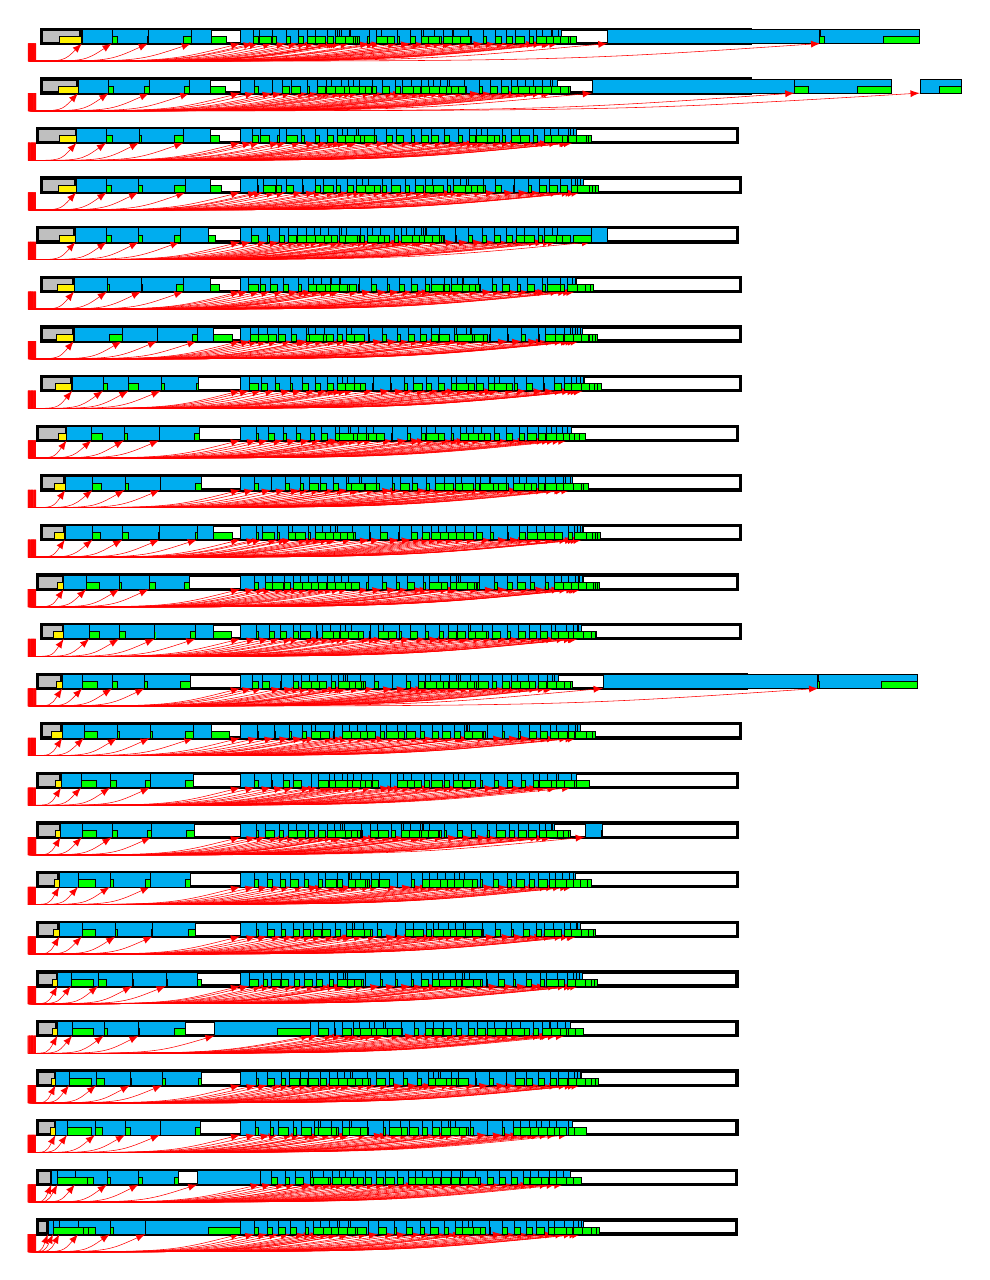
\begin{tikzpicture}[scale=0.9]

%%%%%%%%%%%%%%%%%%% VM 0
\filldraw[draw=black,fill=lightgray,very thick] (0.0,0.0) rectangle (0.141666666667,0.2);
\filldraw[draw=black,fill=white, very thick] (0.141666666667,0.0) rectangle (9.86388888889,0.2);
%%%% JOB 5156
\filldraw[draw=black,fill=cyan, very thin] (7.67222222222,0.0) rectangle (7.69444444444,0.2);
%%%% JOB 5148
\filldraw[draw=black,fill=cyan, very thin] (7.63333333333,0.0) rectangle (7.67222222222,0.2);
%%%% JOB 5127
\filldraw[draw=black,fill=cyan, very thin] (7.55555555556,0.0) rectangle (7.63333333333,0.2);
%%%% JOB 5101
\filldraw[draw=black,fill=cyan, very thin] (7.43611111111,0.0) rectangle (7.55555555556,0.2);
%%%% JOB 5073
\filldraw[draw=black,fill=cyan, very thin] (7.28888888889,0.0) rectangle (7.43611111111,0.2);
%%%% JOB 5049
\filldraw[draw=black,fill=cyan, very thin] (7.20833333333,0.0) rectangle (7.28888888889,0.2);
%%%% JOB 5015
\filldraw[draw=black,fill=cyan, very thin] (7.03888888889,0.0) rectangle (7.20833333333,0.2);
%%%% JOB 4992
\filldraw[draw=black,fill=cyan, very thin] (6.89722222222,0.0) rectangle (7.03888888889,0.2);
%%%% JOB 4964
\filldraw[draw=black,fill=cyan, very thin] (6.72222222222,0.0) rectangle (6.89722222222,0.2);
%%%% JOB 4937
\filldraw[draw=black,fill=cyan, very thin] (6.55555555556,0.0) rectangle (6.72222222222,0.2);
%%%% JOB 4912
\filldraw[draw=black,fill=cyan, very thin] (6.36944444444,0.0) rectangle (6.55555555556,0.2);
%%%% JOB 4879
\filldraw[draw=black,fill=cyan, very thin] (6.13611111111,0.0) rectangle (6.36944444444,0.2);
%%%% JOB 4230
\filldraw[draw=black,fill=cyan, very thin] (1.01666666667,0.0) rectangle (1.51944444444,0.2);
%%%% JOB 4205
\filldraw[draw=black,fill=cyan, very thin] (0.569444444444,0.0) rectangle (1.01666666667,0.2);
%%%% JOB 4865
\filldraw[draw=black,fill=cyan, very thin] (6.06944444444,0.0) rectangle (6.13611111111,0.2);
%%%% JOB 4848
\filldraw[draw=black,fill=cyan, very thin] (5.99444444444,0.0) rectangle (6.06944444444,0.2);
%%%% JOB 4822
\filldraw[draw=black,fill=cyan, very thin] (5.88888888889,0.0) rectangle (5.99444444444,0.2);
%%%% JOB 4793
\filldraw[draw=black,fill=cyan, very thin] (5.73888888889,0.0) rectangle (5.88888888889,0.2);
%%%% JOB 4752
\filldraw[draw=black,fill=cyan, very thin] (5.54166666667,0.0) rectangle (5.73888888889,0.2);
%%%% JOB 4717
\filldraw[draw=black,fill=cyan, very thin] (5.4,0.0) rectangle (5.54166666667,0.2);
%%%% JOB 4689
\filldraw[draw=black,fill=cyan, very thin] (5.2,0.0) rectangle (5.4,0.2);
%%%% JOB 4659
\filldraw[draw=black,fill=cyan, very thin] (5.03055555556,0.0) rectangle (5.2,0.2);
%%%% JOB 4630
\filldraw[draw=black,fill=cyan, very thin] (4.80277777778,0.0) rectangle (5.03055555556,0.2);
%%%% JOB 4605
\filldraw[draw=black,fill=cyan, very thin] (4.66111111111,0.0) rectangle (4.80277777778,0.2);
%%%% JOB 4567
\filldraw[draw=black,fill=cyan, very thin] (4.41388888889,0.0) rectangle (4.66111111111,0.2);
%%%% JOB 4183
\filldraw[draw=black,fill=cyan, very thin] (0.305555555556,0.0) rectangle (0.569444444444,0.2);
%%%% JOB 4560
\filldraw[draw=black,fill=cyan, very thin] (4.38333333333,0.0) rectangle (4.41388888889,0.2);
%%%% JOB 4518
\filldraw[draw=black,fill=cyan, very thin] (4.25277777778,0.0) rectangle (4.38333333333,0.2);
%%%% JOB 4513
\filldraw[draw=black,fill=cyan, very thin] (4.23055555556,0.0) rectangle (4.25277777778,0.2);
%%%% JOB 4487
\filldraw[draw=black,fill=cyan, very thin] (4.11666666667,0.0) rectangle (4.23055555556,0.2);
%%%% JOB 4465
\filldraw[draw=black,fill=cyan, very thin] (3.98611111111,0.0) rectangle (4.11666666667,0.2);
%%%% JOB 4443
\filldraw[draw=black,fill=cyan, very thin] (3.88888888889,0.0) rectangle (3.98611111111,0.2);
%%%% JOB 4422
\filldraw[draw=black,fill=cyan, very thin] (3.77222222222,0.0) rectangle (3.88888888889,0.2);
%%%% JOB 4390
\filldraw[draw=black,fill=cyan, very thin] (3.56111111111,0.0) rectangle (3.77222222222,0.2);
%%%% JOB 4365
\filldraw[draw=black,fill=cyan, very thin] (3.39722222222,0.0) rectangle (3.56111111111,0.2);
%%%% JOB 4345
\filldraw[draw=black,fill=cyan, very thin] (3.23888888889,0.0) rectangle (3.39722222222,0.2);
%%%% JOB 4319
\filldraw[draw=black,fill=cyan, very thin] (3.06111111111,0.0) rectangle (3.23888888889,0.2);
%%%% JOB 4296
\filldraw[draw=black,fill=cyan, very thin] (2.85833333333,0.0) rectangle (3.06111111111,0.2);
%%%% JOB 4175
\filldraw[draw=black,fill=cyan, very thin] (0.216666666667,0.0) rectangle (0.305555555556,0.2);
%%%% JOB 4254
\filldraw[draw=black,fill=cyan, very thin] (1.51944444444,0.0) rectangle (2.85277777778,0.2);
%%%% JOB 4173
\filldraw[draw=black,fill=cyan, very thin] (0.144444444444,0.0) rectangle (0.216666666667,0.2);
\draw[->,color=red,>=latex,very thin] (-0.0277777777778,0.0) -- (-0.0277777777778,-0.25) .. controls (5.10555555556,-0.25) .. (7.67222222222,0.0);
\draw[->,color=red,>=latex,very thin] (-0.0305555555556,0.0) -- (-0.0305555555556,-0.25) .. controls (5.0787037037,-0.25) .. (7.63333333333,0.0);
\draw[->,color=red,>=latex,very thin] (-0.0333333333333,0.0) -- (-0.0333333333333,-0.25) .. controls (5.02592592593,-0.25) .. (7.55555555556,0.0);
\draw[->,color=red,>=latex,very thin] (-0.0361111111111,0.0) -- (-0.0361111111111,-0.25) .. controls (4.94537037037,-0.25) .. (7.43611111111,0.0);
\draw[->,color=red,>=latex,very thin] (-0.0388888888889,0.0) -- (-0.0388888888889,-0.25) .. controls (4.8462962963,-0.25) .. (7.28888888889,0.0);
\draw[->,color=red,>=latex,very thin] (-0.0416666666667,0.0) -- (-0.0416666666667,-0.25) .. controls (4.79166666667,-0.25) .. (7.20833333333,0.0);
\draw[->,color=red,>=latex,very thin] (-0.0444444444444,0.0) -- (-0.0444444444444,-0.25) .. controls (4.67777777778,-0.25) .. (7.03888888889,0.0);
\draw[->,color=red,>=latex,very thin] (-0.0472222222222,0.0) -- (-0.0472222222222,-0.25) .. controls (4.58240740741,-0.25) .. (6.89722222222,0.0);
\draw[->,color=red,>=latex,very thin] (-0.05,0.0) -- (-0.05,-0.25) .. controls (4.46481481481,-0.25) .. (6.72222222222,0.0);
\draw[->,color=red,>=latex,very thin] (-0.0527777777778,0.0) -- (-0.0527777777778,-0.25) .. controls (4.35277777778,-0.25) .. (6.55555555556,0.0);
\draw[->,color=red,>=latex,very thin] (-0.0555555555556,0.0) -- (-0.0555555555556,-0.25) .. controls (4.22777777778,-0.25) .. (6.36944444444,0.0);
\draw[->,color=red,>=latex,very thin] (-0.0583333333333,0.0) -- (-0.0583333333333,-0.25) .. controls (4.0712962963,-0.25) .. (6.13611111111,0.0);
\draw[->,color=red,>=latex,very thin] (-0.0611111111111,0.0) -- (-0.0611111111111,-0.25) .. controls (0.657407407407,-0.25) .. (1.01666666667,0.0);
\draw[->,color=red,>=latex,very thin] (-0.0638888888889,0.0) -- (-0.0638888888889,-0.25) .. controls (0.358333333333,-0.25) .. (0.569444444444,0.0);
\draw[->,color=red,>=latex,very thin] (-0.0666666666667,0.0) -- (-0.0666666666667,-0.25) .. controls (4.02407407407,-0.25) .. (6.06944444444,0.0);
\draw[->,color=red,>=latex,very thin] (-0.0694444444444,0.0) -- (-0.0694444444444,-0.25) .. controls (3.97314814815,-0.25) .. (5.99444444444,0.0);
\draw[->,color=red,>=latex,very thin] (-0.0722222222222,0.0) -- (-0.0722222222222,-0.25) .. controls (3.90185185185,-0.25) .. (5.88888888889,0.0);
\draw[->,color=red,>=latex,very thin] (-0.075,0.0) -- (-0.075,-0.25) .. controls (3.80092592593,-0.25) .. (5.73888888889,0.0);
\draw[->,color=red,>=latex,very thin] (-0.0777777777778,0.0) -- (-0.0777777777778,-0.25) .. controls (3.66851851852,-0.25) .. (5.54166666667,0.0);
\draw[->,color=red,>=latex,very thin] (-0.0805555555556,0.0) -- (-0.0805555555556,-0.25) .. controls (3.57314814815,-0.25) .. (5.4,0.0);
\draw[->,color=red,>=latex,very thin] (-0.0833333333333,0.0) -- (-0.0833333333333,-0.25) .. controls (3.43888888889,-0.25) .. (5.2,0.0);
\draw[->,color=red,>=latex,very thin] (-0.0861111111111,0.0) -- (-0.0861111111111,-0.25) .. controls (3.325,-0.25) .. (5.03055555556,0.0);
\draw[->,color=red,>=latex,very thin] (-0.0888888888889,0.0) -- (-0.0888888888889,-0.25) .. controls (3.17222222222,-0.25) .. (4.80277777778,0.0);
\draw[->,color=red,>=latex,very thin] (-0.0916666666667,0.0) -- (-0.0916666666667,-0.25) .. controls (3.07685185185,-0.25) .. (4.66111111111,0.0);
\draw[->,color=red,>=latex,very thin] (-0.0944444444444,0.0) -- (-0.0944444444444,-0.25) .. controls (2.91111111111,-0.25) .. (4.41388888889,0.0);
\draw[->,color=red,>=latex,very thin] (-0.1,0.0) -- (-0.1,-0.25) .. controls (0.17037037037,-0.25) .. (0.305555555556,0.0);
\draw[->,color=red,>=latex,very thin] (-0.102777777778,0.0) -- (-0.102777777778,-0.25) .. controls (2.88796296296,-0.25) .. (4.38333333333,0.0);
\draw[->,color=red,>=latex,very thin] (-0.105555555556,0.0) -- (-0.105555555556,-0.25) .. controls (2.8,-0.25) .. (4.25277777778,0.0);
\draw[->,color=red,>=latex,very thin] (-0.108333333333,0.0) -- (-0.108333333333,-0.25) .. controls (2.78425925926,-0.25) .. (4.23055555556,0.0);
\draw[->,color=red,>=latex,very thin] (-0.111111111111,0.0) -- (-0.111111111111,-0.25) .. controls (2.70740740741,-0.25) .. (4.11666666667,0.0);
\draw[->,color=red,>=latex,very thin] (-0.113888888889,0.0) -- (-0.113888888889,-0.25) .. controls (2.61944444444,-0.25) .. (3.98611111111,0.0);
\draw[->,color=red,>=latex,very thin] (-0.116666666667,0.0) -- (-0.116666666667,-0.25) .. controls (2.5537037037,-0.25) .. (3.88888888889,0.0);
\draw[->,color=red,>=latex,very thin] (-0.119444444444,0.0) -- (-0.119444444444,-0.25) .. controls (2.475,-0.25) .. (3.77222222222,0.0);
\draw[->,color=red,>=latex,very thin] (-0.122222222222,0.0) -- (-0.122222222222,-0.25) .. controls (2.33333333333,-0.25) .. (3.56111111111,0.0);
\draw[->,color=red,>=latex,very thin] (-0.125,0.0) -- (-0.125,-0.25) .. controls (2.22314814815,-0.25) .. (3.39722222222,0.0);
\draw[->,color=red,>=latex,very thin] (-0.127777777778,0.0) -- (-0.127777777778,-0.25) .. controls (2.11666666667,-0.25) .. (3.23888888889,0.0);
\draw[->,color=red,>=latex,very thin] (-0.130555555556,0.0) -- (-0.130555555556,-0.25) .. controls (1.99722222222,-0.25) .. (3.06111111111,0.0);
\draw[->,color=red,>=latex,very thin] (-0.133333333333,0.0) -- (-0.133333333333,-0.25) .. controls (1.86111111111,-0.25) .. (2.85833333333,0.0);
\draw[->,color=red,>=latex,very thin] (-0.136111111111,0.0) -- (-0.136111111111,-0.25) .. controls (0.0990740740741,-0.25) .. (0.216666666667,0.0);
\draw[->,color=red,>=latex,very thin] (-0.136111111111,0.0) -- (-0.136111111111,-0.25) .. controls (0.967592592593,-0.25) .. (1.51944444444,0.0);
\draw[->,color=red,>=latex,very thin] (-0.138888888889,0.0) -- (-0.138888888889,-0.25) .. controls (0.05,-0.25) .. (0.144444444444,0.0);
\filldraw[draw=black,fill=green,very thin] (7.69444444444,0.0) rectangle (7.92222222222,0.1);
\filldraw[draw=black,fill=green,very thin] (7.67222222222,0.0) rectangle (7.88333333333,0.1);
\filldraw[draw=black,fill=green,very thin] (7.63333333333,0.0) rectangle (7.80555555556,0.1);
\filldraw[draw=black,fill=green,very thin] (7.55555555556,0.0) rectangle (7.68611111111,0.1);
\filldraw[draw=black,fill=green,very thin] (7.43611111111,0.0) rectangle (7.53888888889,0.1);
\filldraw[draw=black,fill=green,very thin] (7.28888888889,0.0) rectangle (7.45833333333,0.1);
\filldraw[draw=black,fill=green,very thin] (7.20833333333,0.0) rectangle (7.28888888889,0.1);
\filldraw[draw=black,fill=green,very thin] (7.03888888889,0.0) rectangle (7.14722222222,0.1);
\filldraw[draw=black,fill=green,very thin] (6.89722222222,0.0) rectangle (6.97222222222,0.1);
\filldraw[draw=black,fill=green,very thin] (6.72222222222,0.0) rectangle (6.80555555556,0.1);
\filldraw[draw=black,fill=green,very thin] (6.55555555556,0.0) rectangle (6.61944444444,0.1);
\filldraw[draw=black,fill=green,very thin] (6.36944444444,0.0) rectangle (6.38611111111,0.1);
\filldraw[draw=black,fill=green,very thin] (1.51944444444,0.0) rectangle (1.51666666667,0.1);
\filldraw[draw=black,fill=green,very thin] (1.01666666667,0.0) rectangle (1.06944444444,0.1);
\filldraw[draw=black,fill=green,very thin] (6.13611111111,0.0) rectangle (6.31944444444,0.1);
\filldraw[draw=black,fill=green,very thin] (6.06944444444,0.0) rectangle (6.24444444444,0.1);
\filldraw[draw=black,fill=green,very thin] (5.99444444444,0.0) rectangle (6.13888888889,0.1);
\filldraw[draw=black,fill=green,very thin] (5.88888888889,0.0) rectangle (5.98888888889,0.1);
\filldraw[draw=black,fill=green,very thin] (5.73888888889,0.0) rectangle (5.79166666667,0.1);
\filldraw[draw=black,fill=green,very thin] (5.54166666667,0.0) rectangle (5.65,0.1);
\filldraw[draw=black,fill=green,very thin] (5.4,0.0) rectangle (5.45,0.1);
\filldraw[draw=black,fill=green,very thin] (5.2,0.0) rectangle (5.28055555556,0.1);
\filldraw[draw=black,fill=green,very thin] (5.03055555556,0.0) rectangle (5.05277777778,0.1);
\filldraw[draw=black,fill=green,very thin] (4.80277777778,0.0) rectangle (4.91111111111,0.1);
\filldraw[draw=black,fill=green,very thin] (4.66111111111,0.0) rectangle (4.66388888889,0.1);
\filldraw[draw=black,fill=green,very thin] (0.569444444444,0.0) rectangle (0.805555555556,0.1);
\filldraw[draw=black,fill=green,very thin] (4.41388888889,0.0) rectangle (4.63333333333,0.1);
\filldraw[draw=black,fill=green,very thin] (4.38333333333,0.0) rectangle (4.50277777778,0.1);
\filldraw[draw=black,fill=green,very thin] (4.25277777778,0.0) rectangle (4.48055555556,0.1);
\filldraw[draw=black,fill=green,very thin] (4.23055555556,0.0) rectangle (4.36666666667,0.1);
\filldraw[draw=black,fill=green,very thin] (4.11666666667,0.0) rectangle (4.23611111111,0.1);
\filldraw[draw=black,fill=green,very thin] (3.98611111111,0.0) rectangle (4.13888888889,0.1);
\filldraw[draw=black,fill=green,very thin] (3.88888888889,0.0) rectangle (4.02222222222,0.1);
\filldraw[draw=black,fill=green,very thin] (3.77222222222,0.0) rectangle (3.81111111111,0.1);
\filldraw[draw=black,fill=green,very thin] (3.56111111111,0.0) rectangle (3.64722222222,0.1);
\filldraw[draw=black,fill=green,very thin] (3.39722222222,0.0) rectangle (3.48888888889,0.1);
\filldraw[draw=black,fill=green,very thin] (3.23888888889,0.0) rectangle (3.31111111111,0.1);
\filldraw[draw=black,fill=green,very thin] (3.06111111111,0.0) rectangle (3.10833333333,0.1);
\filldraw[draw=black,fill=green,very thin] (0.305555555556,0.0) rectangle (0.716666666667,0.1);
\filldraw[draw=black,fill=green,very thin] (2.85277777778,0.0) rectangle (2.40833333333,0.1);
\filldraw[draw=black,fill=green,very thin] (0.216666666667,0.0) rectangle (0.644444444444,0.1);
\filldraw[draw=black,fill=yellow,very thin] (0.147222222222,0.0) rectangle (0.141666666667,0.1);

%%%%%%%%%%%%%%%%%%% VM 1
\filldraw[draw=black,fill=lightgray,very thick] (0.0,0.7) rectangle (0.188888888889,0.9);
\filldraw[draw=black,fill=white, very thick] (0.188888888889,0.7) rectangle (9.86388888889,0.9);
%%%% JOB 5096
\filldraw[draw=black,fill=cyan, very thin] (7.41944444444,0.7) rectangle (7.50833333333,0.9);
%%%% JOB 5079
\filldraw[draw=black,fill=cyan, very thin] (7.31111111111,0.7) rectangle (7.41944444444,0.9);
%%%% JOB 5053
\filldraw[draw=black,fill=cyan, very thin] (7.21388888889,0.7) rectangle (7.31111111111,0.9);
%%%% JOB 5023
\filldraw[draw=black,fill=cyan, very thin] (7.06666666667,0.7) rectangle (7.21388888889,0.9);
%%%% JOB 5005
\filldraw[draw=black,fill=cyan, very thin] (6.94722222222,0.7) rectangle (7.06666666667,0.9);
%%%% JOB 4986
\filldraw[draw=black,fill=cyan, very thin] (6.85277777778,0.7) rectangle (6.94722222222,0.9);
%%%% JOB 4959
\filldraw[draw=black,fill=cyan, very thin] (6.68611111111,0.7) rectangle (6.85277777778,0.9);
%%%% JOB 4933
\filldraw[draw=black,fill=cyan, very thin] (6.51666666667,0.7) rectangle (6.68611111111,0.9);
%%%% JOB 4908
\filldraw[draw=black,fill=cyan, very thin] (6.34722222222,0.7) rectangle (6.51666666667,0.9);
%%%% JOB 4882
\filldraw[draw=black,fill=cyan, very thin] (6.17777777778,0.7) rectangle (6.34722222222,0.9);
%%%% JOB 4846
\filldraw[draw=black,fill=cyan, very thin] (5.98888888889,0.7) rectangle (6.17777777778,0.9);
%%%% JOB 4250
\filldraw[draw=black,fill=cyan, very thin] (1.425,0.7) rectangle (1.98888888889,0.9);
%%%% JOB 4226
\filldraw[draw=black,fill=cyan, very thin] (0.977777777778,0.7) rectangle (1.425,0.9);
%%%% JOB 4843
\filldraw[draw=black,fill=cyan, very thin] (5.96111111111,0.7) rectangle (5.98888888889,0.9);
%%%% JOB 4808
\filldraw[draw=black,fill=cyan, very thin] (5.83055555556,0.7) rectangle (5.96111111111,0.9);
%%%% JOB 4784
\filldraw[draw=black,fill=cyan, very thin] (5.7,0.7) rectangle (5.83055555556,0.9);
%%%% JOB 4761
\filldraw[draw=black,fill=cyan, very thin] (5.56944444444,0.7) rectangle (5.7,0.9);
%%%% JOB 4728
\filldraw[draw=black,fill=cyan, very thin] (5.42777777778,0.7) rectangle (5.56944444444,0.9);
%%%% JOB 4712
\filldraw[draw=black,fill=cyan, very thin] (5.33055555556,0.7) rectangle (5.42777777778,0.9);
%%%% JOB 4693
\filldraw[draw=black,fill=cyan, very thin] (5.23055555556,0.7) rectangle (5.33055555556,0.9);
%%%% JOB 4669
\filldraw[draw=black,fill=cyan, very thin] (5.075,0.7) rectangle (5.23055555556,0.9);
%%%% JOB 4646
\filldraw[draw=black,fill=cyan, very thin] (4.90555555556,0.7) rectangle (5.075,0.9);
%%%% JOB 4625
\filldraw[draw=black,fill=cyan, very thin] (4.775,0.7) rectangle (4.90555555556,0.9);
%%%% JOB 4599
\filldraw[draw=black,fill=cyan, very thin] (4.62222222222,0.7) rectangle (4.775,0.9);
%%%% JOB 4282
\filldraw[draw=black,fill=cyan, very thin] (2.25555555556,0.7) rectangle (3.13611111111,0.9);
%%%% JOB 4578
\filldraw[draw=black,fill=cyan, very thin] (4.45833333333,0.7) rectangle (4.62222222222,0.9);
%%%% JOB 4200
\filldraw[draw=black,fill=cyan, very thin] (0.525,0.7) rectangle (0.977777777778,0.9);
%%%% JOB 4541
\filldraw[draw=black,fill=cyan, very thin] (4.33888888889,0.7) rectangle (4.45833333333,0.9);
%%%% JOB 4521
\filldraw[draw=black,fill=cyan, very thin] (4.25833333333,0.7) rectangle (4.33888888889,0.9);
%%%% JOB 4495
\filldraw[draw=black,fill=cyan, very thin] (4.15555555556,0.7) rectangle (4.25833333333,0.9);
%%%% JOB 4474
\filldraw[draw=black,fill=cyan, very thin] (4.03333333333,0.7) rectangle (4.15555555556,0.9);
%%%% JOB 4440
\filldraw[draw=black,fill=cyan, very thin] (3.87777777778,0.7) rectangle (4.03333333333,0.9);
%%%% JOB 4437
\filldraw[draw=black,fill=cyan, very thin] (3.85,0.7) rectangle (3.87777777778,0.9);
%%%% JOB 4403
\filldraw[draw=black,fill=cyan, very thin] (3.63611111111,0.7) rectangle (3.85,0.9);
%%%% JOB 4380
\filldraw[draw=black,fill=cyan, very thin] (3.49166666667,0.7) rectangle (3.63611111111,0.9);
%%%% JOB 4355
\filldraw[draw=black,fill=cyan, very thin] (3.3,0.7) rectangle (3.49166666667,0.9);
%%%% JOB 4333
\filldraw[draw=black,fill=cyan, very thin] (3.13611111111,0.7) rectangle (3.3,0.9);
%%%% JOB 4180
\filldraw[draw=black,fill=cyan, very thin] (0.277777777778,0.7) rectangle (0.525,0.9);
%%%% JOB 4174
\filldraw[draw=black,fill=cyan, very thin] (0.194444444444,0.7) rectangle (0.277777777778,0.9);
\draw[->,color=red,>=latex,very thin] (-0.0305555555556,0.7) -- (-0.0305555555556,0.45) .. controls (4.93611111111,0.45) .. (7.41944444444,0.7);
\draw[->,color=red,>=latex,very thin] (-0.0333333333333,0.7) -- (-0.0333333333333,0.45) .. controls (4.86296296296,0.45) .. (7.31111111111,0.7);
\draw[->,color=red,>=latex,very thin] (-0.0361111111111,0.7) -- (-0.0361111111111,0.45) .. controls (4.79722222222,0.45) .. (7.21388888889,0.7);
\draw[->,color=red,>=latex,very thin] (-0.0388888888889,0.7) -- (-0.0388888888889,0.45) .. controls (4.69814814815,0.45) .. (7.06666666667,0.7);
\draw[->,color=red,>=latex,very thin] (-0.0416666666667,0.7) -- (-0.0416666666667,0.45) .. controls (4.61759259259,0.45) .. (6.94722222222,0.7);
\draw[->,color=red,>=latex,very thin] (-0.0444444444444,0.7) -- (-0.0444444444444,0.45) .. controls (4.5537037037,0.45) .. (6.85277777778,0.7);
\draw[->,color=red,>=latex,very thin] (-0.0472222222222,0.7) -- (-0.0472222222222,0.45) .. controls (4.44166666667,0.45) .. (6.68611111111,0.7);
\draw[->,color=red,>=latex,very thin] (-0.05,0.7) -- (-0.05,0.45) .. controls (4.32777777778,0.45) .. (6.51666666667,0.7);
\draw[->,color=red,>=latex,very thin] (-0.0527777777778,0.7) -- (-0.0527777777778,0.45) .. controls (4.21388888889,0.45) .. (6.34722222222,0.7);
\draw[->,color=red,>=latex,very thin] (-0.0555555555556,0.7) -- (-0.0555555555556,0.45) .. controls (4.1,0.45) .. (6.17777777778,0.7);
\draw[->,color=red,>=latex,very thin] (-0.0583333333333,0.7) -- (-0.0583333333333,0.45) .. controls (3.97314814815,0.45) .. (5.98888888889,0.7);
\draw[->,color=red,>=latex,very thin] (-0.0611111111111,0.7) -- (-0.0611111111111,0.45) .. controls (0.92962962963,0.45) .. (1.425,0.7);
\draw[->,color=red,>=latex,very thin] (-0.0638888888889,0.7) -- (-0.0638888888889,0.45) .. controls (0.630555555556,0.45) .. (0.977777777778,0.7);
\draw[->,color=red,>=latex,very thin] (-0.0666666666667,0.7) -- (-0.0666666666667,0.45) .. controls (3.95185185185,0.45) .. (5.96111111111,0.7);
\draw[->,color=red,>=latex,very thin] (-0.0694444444444,0.7) -- (-0.0694444444444,0.45) .. controls (3.86388888889,0.45) .. (5.83055555556,0.7);
\draw[->,color=red,>=latex,very thin] (-0.0722222222222,0.7) -- (-0.0722222222222,0.45) .. controls (3.77592592593,0.45) .. (5.7,0.7);
\draw[->,color=red,>=latex,very thin] (-0.075,0.7) -- (-0.075,0.45) .. controls (3.68796296296,0.45) .. (5.56944444444,0.7);
\draw[->,color=red,>=latex,very thin] (-0.0777777777778,0.7) -- (-0.0777777777778,0.45) .. controls (3.59259259259,0.45) .. (5.42777777778,0.7);
\draw[->,color=red,>=latex,very thin] (-0.0805555555556,0.7) -- (-0.0805555555556,0.45) .. controls (3.52685185185,0.45) .. (5.33055555556,0.7);
\draw[->,color=red,>=latex,very thin] (-0.0833333333333,0.7) -- (-0.0833333333333,0.45) .. controls (3.45925925926,0.45) .. (5.23055555556,0.7);
\draw[->,color=red,>=latex,very thin] (-0.0861111111111,0.7) -- (-0.0861111111111,0.45) .. controls (3.35462962963,0.45) .. (5.075,0.7);
\draw[->,color=red,>=latex,very thin] (-0.0888888888889,0.7) -- (-0.0888888888889,0.45) .. controls (3.24074074074,0.45) .. (4.90555555556,0.7);
\draw[->,color=red,>=latex,very thin] (-0.0916666666667,0.7) -- (-0.0916666666667,0.45) .. controls (3.15277777778,0.45) .. (4.775,0.7);
\draw[->,color=red,>=latex,very thin] (-0.0944444444444,0.7) -- (-0.0944444444444,0.45) .. controls (3.05,0.45) .. (4.62222222222,0.7);
\draw[->,color=red,>=latex,very thin] (-0.0972222222222,0.7) -- (-0.0972222222222,0.45) .. controls (1.4712962963,0.45) .. (2.25555555556,0.7);
\draw[->,color=red,>=latex,very thin] (-0.0972222222222,0.7) -- (-0.0972222222222,0.45) .. controls (2.93981481481,0.45) .. (4.45833333333,0.7);
\draw[->,color=red,>=latex,very thin] (-0.1,0.7) -- (-0.1,0.45) .. controls (0.316666666667,0.45) .. (0.525,0.7);
\draw[->,color=red,>=latex,very thin] (-0.105555555556,0.7) -- (-0.105555555556,0.45) .. controls (2.85740740741,0.45) .. (4.33888888889,0.7);
\draw[->,color=red,>=latex,very thin] (-0.108333333333,0.7) -- (-0.108333333333,0.45) .. controls (2.80277777778,0.45) .. (4.25833333333,0.7);
\draw[->,color=red,>=latex,very thin] (-0.111111111111,0.7) -- (-0.111111111111,0.45) .. controls (2.73333333333,0.45) .. (4.15555555556,0.7);
\draw[->,color=red,>=latex,very thin] (-0.113888888889,0.7) -- (-0.113888888889,0.45) .. controls (2.65092592593,0.45) .. (4.03333333333,0.7);
\draw[->,color=red,>=latex,very thin] (-0.116666666667,0.7) -- (-0.116666666667,0.45) .. controls (2.5462962963,0.45) .. (3.87777777778,0.7);
\draw[->,color=red,>=latex,very thin] (-0.119444444444,0.7) -- (-0.119444444444,0.45) .. controls (2.52685185185,0.45) .. (3.85,0.7);
\draw[->,color=red,>=latex,very thin] (-0.122222222222,0.7) -- (-0.122222222222,0.45) .. controls (2.38333333333,0.45) .. (3.63611111111,0.7);
\draw[->,color=red,>=latex,very thin] (-0.125,0.7) -- (-0.125,0.45) .. controls (2.28611111111,0.45) .. (3.49166666667,0.7);
\draw[->,color=red,>=latex,very thin] (-0.127777777778,0.7) -- (-0.127777777778,0.45) .. controls (2.15740740741,0.45) .. (3.3,0.7);
\draw[->,color=red,>=latex,very thin] (-0.130555555556,0.7) -- (-0.130555555556,0.45) .. controls (2.04722222222,0.45) .. (3.13611111111,0.7);
\draw[->,color=red,>=latex,very thin] (-0.136111111111,0.7) -- (-0.136111111111,0.45) .. controls (0.139814814815,0.45) .. (0.277777777778,0.7);
\draw[->,color=red,>=latex,very thin] (-0.138888888889,0.7) -- (-0.138888888889,0.45) .. controls (0.0833333333333,0.45) .. (0.194444444444,0.7);
\filldraw[draw=black,fill=green,very thin] (7.50833333333,0.7) rectangle (7.66944444444,0.8);
\filldraw[draw=black,fill=green,very thin] (7.41944444444,0.7) rectangle (7.56111111111,0.8);
\filldraw[draw=black,fill=green,very thin] (7.31111111111,0.7) rectangle (7.46388888889,0.8);
\filldraw[draw=black,fill=green,very thin] (7.21388888889,0.7) rectangle (7.31666666667,0.8);
\filldraw[draw=black,fill=green,very thin] (7.06666666667,0.7) rectangle (7.19722222222,0.8);
\filldraw[draw=black,fill=green,very thin] (6.94722222222,0.7) rectangle (7.10277777778,0.8);
\filldraw[draw=black,fill=green,very thin] (6.85277777778,0.7) rectangle (6.93611111111,0.8);
\filldraw[draw=black,fill=green,very thin] (6.68611111111,0.7) rectangle (6.76666666667,0.8);
\filldraw[draw=black,fill=green,very thin] (6.51666666667,0.7) rectangle (6.59722222222,0.8);
\filldraw[draw=black,fill=green,very thin] (6.34722222222,0.7) rectangle (6.42777777778,0.8);
\filldraw[draw=black,fill=green,very thin] (6.17777777778,0.7) rectangle (6.23888888889,0.8);
\filldraw[draw=black,fill=green,very thin] (1.98888888889,0.7) rectangle (1.925,0.8);
\filldraw[draw=black,fill=green,very thin] (1.425,0.7) rectangle (1.47777777778,0.8);
\filldraw[draw=black,fill=green,very thin] (5.98888888889,0.7) rectangle (6.21111111111,0.8);
\filldraw[draw=black,fill=green,very thin] (5.96111111111,0.7) rectangle (6.08055555556,0.8);
\filldraw[draw=black,fill=green,very thin] (5.83055555556,0.7) rectangle (5.95,0.8);
\filldraw[draw=black,fill=green,very thin] (5.7,0.7) rectangle (5.81944444444,0.8);
\filldraw[draw=black,fill=green,very thin] (5.56944444444,0.7) rectangle (5.67777777778,0.8);
\filldraw[draw=black,fill=green,very thin] (5.42777777778,0.7) rectangle (5.58055555556,0.8);
\filldraw[draw=black,fill=green,very thin] (5.33055555556,0.7) rectangle (5.48055555556,0.8);
\filldraw[draw=black,fill=green,very thin] (5.23055555556,0.7) rectangle (5.325,0.8);
\filldraw[draw=black,fill=green,very thin] (5.075,0.7) rectangle (5.15555555556,0.8);
\filldraw[draw=black,fill=green,very thin] (4.90555555556,0.7) rectangle (5.025,0.8);
\filldraw[draw=black,fill=green,very thin] (4.775,0.7) rectangle (4.87222222222,0.8);
\filldraw[draw=black,fill=green,very thin] (3.13611111111,0.7) rectangle (3.14444444444,0.8);
\filldraw[draw=black,fill=green,very thin] (4.62222222222,0.7) rectangle (4.70833333333,0.8);
\filldraw[draw=black,fill=green,very thin] (0.977777777778,0.7) rectangle (1.025,0.8);
\filldraw[draw=black,fill=green,very thin] (4.45833333333,0.7) rectangle (4.58888888889,0.8);
\filldraw[draw=black,fill=green,very thin] (4.33888888889,0.7) rectangle (4.50833333333,0.8);
\filldraw[draw=black,fill=green,very thin] (4.25833333333,0.7) rectangle (4.40555555556,0.8);
\filldraw[draw=black,fill=green,very thin] (4.15555555556,0.7) rectangle (4.28333333333,0.8);
\filldraw[draw=black,fill=green,very thin] (4.03333333333,0.7) rectangle (4.12777777778,0.8);
\filldraw[draw=black,fill=green,very thin] (3.87777777778,0.7) rectangle (4.1,0.8);
\filldraw[draw=black,fill=green,very thin] (3.85,0.7) rectangle (3.88611111111,0.8);
\filldraw[draw=black,fill=green,very thin] (3.63611111111,0.7) rectangle (3.74166666667,0.8);
\filldraw[draw=black,fill=green,very thin] (3.49166666667,0.7) rectangle (3.55,0.8);
\filldraw[draw=black,fill=green,very thin] (3.3,0.7) rectangle (3.38611111111,0.8);
\filldraw[draw=black,fill=green,very thin] (0.525,0.7) rectangle (0.777777777778,0.8);
\filldraw[draw=black,fill=green,very thin] (0.277777777778,0.7) rectangle (0.694444444444,0.8);
\filldraw[draw=black,fill=yellow,very thin] (0.169444444444,0.7) rectangle (0.188888888889,0.8);

%%%%%%%%%%%%%%%%%%% VM 2
\filldraw[draw=black,fill=lightgray,very thick] (0.0,1.4) rectangle (0.247222222222,1.6);
\filldraw[draw=black,fill=white, very thick] (0.247222222222,1.4) rectangle (9.86666666667,1.6);
%%%% JOB 5109
\filldraw[draw=black,fill=cyan, very thin] (7.48611111111,1.4) rectangle (7.53611111111,1.6);
%%%% JOB 5083
\filldraw[draw=black,fill=cyan, very thin] (7.32222222222,1.4) rectangle (7.48611111111,1.6);
%%%% JOB 5052
\filldraw[draw=black,fill=cyan, very thin] (7.21388888889,1.4) rectangle (7.32222222222,1.6);
%%%% JOB 5030
\filldraw[draw=black,fill=cyan, very thin] (7.10555555556,1.4) rectangle (7.21388888889,1.6);
%%%% JOB 5014
\filldraw[draw=black,fill=cyan, very thin] (7.03888888889,1.4) rectangle (7.10555555556,1.6);
%%%% JOB 5002
\filldraw[draw=black,fill=cyan, very thin] (6.94166666667,1.4) rectangle (7.03888888889,1.6);
%%%% JOB 4981
\filldraw[draw=black,fill=cyan, very thin] (6.80555555556,1.4) rectangle (6.94166666667,1.6);
%%%% JOB 4960
\filldraw[draw=black,fill=cyan, very thin] (6.70277777778,1.4) rectangle (6.80555555556,1.6);
%%%% JOB 4936
\filldraw[draw=black,fill=cyan, very thin] (6.55555555556,1.4) rectangle (6.70277777778,1.6);
%%%% JOB 4903
\filldraw[draw=black,fill=cyan, very thin] (6.33611111111,1.4) rectangle (6.55555555556,1.6);
%%%% JOB 4873
\filldraw[draw=black,fill=cyan, very thin] (6.09722222222,1.4) rectangle (6.33611111111,1.6);
%%%% JOB 4267
\filldraw[draw=black,fill=cyan, very thin] (1.725,1.4) rectangle (2.29444444444,1.6);
%%%% JOB 4821
\filldraw[draw=black,fill=cyan, very thin] (5.88888888889,1.4) rectangle (6.09722222222,1.6);
%%%% JOB 4243
\filldraw[draw=black,fill=cyan, very thin] (1.23333333333,1.4) rectangle (1.725,1.6);
%%%% JOB 4805
\filldraw[draw=black,fill=cyan, very thin] (5.81944444444,1.4) rectangle (5.88888888889,1.6);
%%%% JOB 4801
\filldraw[draw=black,fill=cyan, very thin] (5.79722222222,1.4) rectangle (5.81944444444,1.6);
%%%% JOB 4783
\filldraw[draw=black,fill=cyan, very thin] (5.7,1.4) rectangle (5.79722222222,1.6);
%%%% JOB 4759
\filldraw[draw=black,fill=cyan, very thin] (5.56388888889,1.4) rectangle (5.7,1.6);
%%%% JOB 4726
\filldraw[draw=black,fill=cyan, very thin] (5.42222222222,1.4) rectangle (5.56388888889,1.6);
%%%% JOB 4695
\filldraw[draw=black,fill=cyan, very thin] (5.24722222222,1.4) rectangle (5.42222222222,1.6);
%%%% JOB 4676
\filldraw[draw=black,fill=cyan, very thin] (5.11666666667,1.4) rectangle (5.24722222222,1.6);
%%%% JOB 4651
\filldraw[draw=black,fill=cyan, very thin] (4.96388888889,1.4) rectangle (5.11666666667,1.6);
%%%% JOB 4643
\filldraw[draw=black,fill=cyan, very thin] (4.87777777778,1.4) rectangle (4.96388888889,1.6);
%%%% JOB 4604
\filldraw[draw=black,fill=cyan, very thin] (4.65555555556,1.4) rectangle (4.87777777778,1.6);
%%%% JOB 4568
\filldraw[draw=black,fill=cyan, very thin] (4.41944444444,1.4) rectangle (4.65555555556,1.6);
%%%% JOB 4218
\filldraw[draw=black,fill=cyan, very thin] (0.808333333333,1.4) rectangle (1.23333333333,1.6);
%%%% JOB 4561
\filldraw[draw=black,fill=cyan, very thin] (4.39444444444,1.4) rectangle (4.41944444444,1.6);
%%%% JOB 4534
\filldraw[draw=black,fill=cyan, very thin] (4.3,1.4) rectangle (4.39444444444,1.6);
%%%% JOB 4492
\filldraw[draw=black,fill=cyan, very thin] (4.14444444444,1.4) rectangle (4.3,1.6);
%%%% JOB 4464
\filldraw[draw=black,fill=cyan, very thin] (3.98611111111,1.4) rectangle (4.14444444444,1.6);
%%%% JOB 4461
\filldraw[draw=black,fill=cyan, very thin] (3.95833333333,1.4) rectangle (3.98611111111,1.6);
%%%% JOB 4445
\filldraw[draw=black,fill=cyan, very thin] (3.89444444444,1.4) rectangle (3.95833333333,1.6);
%%%% JOB 4413
\filldraw[draw=black,fill=cyan, very thin] (3.71388888889,1.4) rectangle (3.89444444444,1.6);
%%%% JOB 4399
\filldraw[draw=black,fill=cyan, very thin] (3.60555555556,1.4) rectangle (3.71388888889,1.6);
%%%% JOB 4363
\filldraw[draw=black,fill=cyan, very thin] (3.39166666667,1.4) rectangle (3.60555555556,1.6);
%%%% JOB 4350
\filldraw[draw=black,fill=cyan, very thin] (3.27777777778,1.4) rectangle (3.39166666667,1.6);
%%%% JOB 4321
\filldraw[draw=black,fill=cyan, very thin] (3.075,1.4) rectangle (3.27777777778,1.6);
%%%% JOB 4295
\filldraw[draw=black,fill=cyan, very thin] (2.85833333333,1.4) rectangle (3.075,1.6);
%%%% JOB 4193
\filldraw[draw=black,fill=cyan, very thin] (0.413888888889,1.4) rectangle (0.808333333333,1.6);
%%%% JOB 4177
\filldraw[draw=black,fill=cyan, very thin] (0.25,1.4) rectangle (0.413888888889,1.6);
\draw[->,color=red,>=latex,very thin] (-0.0305555555556,1.4) -- (-0.0305555555556,1.15) .. controls (4.98055555556,1.15) .. (7.48611111111,1.4);
\draw[->,color=red,>=latex,very thin] (-0.0333333333333,1.4) -- (-0.0333333333333,1.15) .. controls (4.87037037037,1.15) .. (7.32222222222,1.4);
\draw[->,color=red,>=latex,very thin] (-0.0361111111111,1.4) -- (-0.0361111111111,1.15) .. controls (4.79722222222,1.15) .. (7.21388888889,1.4);
\draw[->,color=red,>=latex,very thin] (-0.0388888888889,1.4) -- (-0.0388888888889,1.15) .. controls (4.72407407407,1.15) .. (7.10555555556,1.4);
\draw[->,color=red,>=latex,very thin] (-0.0416666666667,1.4) -- (-0.0416666666667,1.15) .. controls (4.6787037037,1.15) .. (7.03888888889,1.4);
\draw[->,color=red,>=latex,very thin] (-0.0444444444444,1.4) -- (-0.0444444444444,1.15) .. controls (4.61296296296,1.15) .. (6.94166666667,1.4);
\draw[->,color=red,>=latex,very thin] (-0.0472222222222,1.4) -- (-0.0472222222222,1.15) .. controls (4.5212962963,1.15) .. (6.80555555556,1.4);
\draw[->,color=red,>=latex,very thin] (-0.05,1.4) -- (-0.05,1.15) .. controls (4.45185185185,1.15) .. (6.70277777778,1.4);
\draw[->,color=red,>=latex,very thin] (-0.0527777777778,1.4) -- (-0.0527777777778,1.15) .. controls (4.35277777778,1.15) .. (6.55555555556,1.4);
\draw[->,color=red,>=latex,very thin] (-0.0555555555556,1.4) -- (-0.0555555555556,1.15) .. controls (4.20555555556,1.15) .. (6.33611111111,1.4);
\draw[->,color=red,>=latex,very thin] (-0.0583333333333,1.4) -- (-0.0583333333333,1.15) .. controls (4.04537037037,1.15) .. (6.09722222222,1.4);
\draw[->,color=red,>=latex,very thin] (-0.0611111111111,1.4) -- (-0.0611111111111,1.15) .. controls (1.12962962963,1.15) .. (1.725,1.4);
\draw[->,color=red,>=latex,very thin] (-0.0611111111111,1.4) -- (-0.0611111111111,1.15) .. controls (3.90555555556,1.15) .. (5.88888888889,1.4);
\draw[->,color=red,>=latex,very thin] (-0.0638888888889,1.4) -- (-0.0638888888889,1.15) .. controls (0.800925925926,1.15) .. (1.23333333333,1.4);
\draw[->,color=red,>=latex,very thin] (-0.0666666666667,1.4) -- (-0.0666666666667,1.15) .. controls (3.85740740741,1.15) .. (5.81944444444,1.4);
\draw[->,color=red,>=latex,very thin] (-0.0694444444444,1.4) -- (-0.0694444444444,1.15) .. controls (3.84166666667,1.15) .. (5.79722222222,1.4);
\draw[->,color=red,>=latex,very thin] (-0.0722222222222,1.4) -- (-0.0722222222222,1.15) .. controls (3.77592592593,1.15) .. (5.7,1.4);
\draw[->,color=red,>=latex,very thin] (-0.075,1.4) -- (-0.075,1.15) .. controls (3.68425925926,1.15) .. (5.56388888889,1.4);
\draw[->,color=red,>=latex,very thin] (-0.0777777777778,1.4) -- (-0.0777777777778,1.15) .. controls (3.58888888889,1.15) .. (5.42222222222,1.4);
\draw[->,color=red,>=latex,very thin] (-0.0805555555556,1.4) -- (-0.0805555555556,1.15) .. controls (3.4712962963,1.15) .. (5.24722222222,1.4);
\draw[->,color=red,>=latex,very thin] (-0.0833333333333,1.4) -- (-0.0833333333333,1.15) .. controls (3.38333333333,1.15) .. (5.11666666667,1.4);
\draw[->,color=red,>=latex,very thin] (-0.0861111111111,1.4) -- (-0.0861111111111,1.15) .. controls (3.28055555556,1.15) .. (4.96388888889,1.4);
\draw[->,color=red,>=latex,very thin] (-0.0888888888889,1.4) -- (-0.0888888888889,1.15) .. controls (3.22222222222,1.15) .. (4.87777777778,1.4);
\draw[->,color=red,>=latex,very thin] (-0.0916666666667,1.4) -- (-0.0916666666667,1.15) .. controls (3.07314814815,1.15) .. (4.65555555556,1.4);
\draw[->,color=red,>=latex,very thin] (-0.0944444444444,1.4) -- (-0.0944444444444,1.15) .. controls (2.91481481481,1.15) .. (4.41944444444,1.4);
\draw[->,color=red,>=latex,very thin] (-0.1,1.4) -- (-0.1,1.15) .. controls (0.505555555556,1.15) .. (0.808333333333,1.4);
\draw[->,color=red,>=latex,very thin] (-0.102777777778,1.4) -- (-0.102777777778,1.15) .. controls (2.89537037037,1.15) .. (4.39444444444,1.4);
\draw[->,color=red,>=latex,very thin] (-0.105555555556,1.4) -- (-0.105555555556,1.15) .. controls (2.83148148148,1.15) .. (4.3,1.4);
\draw[->,color=red,>=latex,very thin] (-0.108333333333,1.4) -- (-0.108333333333,1.15) .. controls (2.72685185185,1.15) .. (4.14444444444,1.4);
\draw[->,color=red,>=latex,very thin] (-0.111111111111,1.4) -- (-0.111111111111,1.15) .. controls (2.62037037037,1.15) .. (3.98611111111,1.4);
\draw[->,color=red,>=latex,very thin] (-0.113888888889,1.4) -- (-0.113888888889,1.15) .. controls (2.60092592593,1.15) .. (3.95833333333,1.4);
\draw[->,color=red,>=latex,very thin] (-0.116666666667,1.4) -- (-0.116666666667,1.15) .. controls (2.55740740741,1.15) .. (3.89444444444,1.4);
\draw[->,color=red,>=latex,very thin] (-0.119444444444,1.4) -- (-0.119444444444,1.15) .. controls (2.43611111111,1.15) .. (3.71388888889,1.4);
\draw[->,color=red,>=latex,very thin] (-0.122222222222,1.4) -- (-0.122222222222,1.15) .. controls (2.36296296296,1.15) .. (3.60555555556,1.4);
\draw[->,color=red,>=latex,very thin] (-0.125,1.4) -- (-0.125,1.15) .. controls (2.21944444444,1.15) .. (3.39166666667,1.4);
\draw[->,color=red,>=latex,very thin] (-0.127777777778,1.4) -- (-0.127777777778,1.15) .. controls (2.14259259259,1.15) .. (3.27777777778,1.4);
\draw[->,color=red,>=latex,very thin] (-0.130555555556,1.4) -- (-0.130555555556,1.15) .. controls (2.00648148148,1.15) .. (3.075,1.4);
\draw[->,color=red,>=latex,very thin] (-0.133333333333,1.4) -- (-0.133333333333,1.15) .. controls (1.86111111111,1.15) .. (2.85833333333,1.4);
\draw[->,color=red,>=latex,very thin] (-0.136111111111,1.4) -- (-0.136111111111,1.15) .. controls (0.230555555556,1.15) .. (0.413888888889,1.4);
\draw[->,color=red,>=latex,very thin] (-0.138888888889,1.4) -- (-0.138888888889,1.15) .. controls (0.12037037037,1.15) .. (0.25,1.4);
\filldraw[draw=black,fill=green,very thin] (7.53611111111,1.4) rectangle (7.73611111111,1.5);
\filldraw[draw=black,fill=green,very thin] (7.48611111111,1.4) rectangle (7.57222222222,1.5);
\filldraw[draw=black,fill=green,very thin] (7.32222222222,1.4) rectangle (7.46388888889,1.5);
\filldraw[draw=black,fill=green,very thin] (7.21388888889,1.4) rectangle (7.35555555556,1.5);
\filldraw[draw=black,fill=green,very thin] (7.10555555556,1.4) rectangle (7.28888888889,1.5);
\filldraw[draw=black,fill=green,very thin] (7.03888888889,1.4) rectangle (7.19166666667,1.5);
\filldraw[draw=black,fill=green,very thin] (6.94166666667,1.4) rectangle (7.05555555556,1.5);
\filldraw[draw=black,fill=green,very thin] (6.80555555556,1.4) rectangle (6.95277777778,1.5);
\filldraw[draw=black,fill=green,very thin] (6.70277777778,1.4) rectangle (6.80555555556,1.5);
\filldraw[draw=black,fill=green,very thin] (6.55555555556,1.4) rectangle (6.58611111111,1.5);
\filldraw[draw=black,fill=green,very thin] (6.33611111111,1.4) rectangle (6.34722222222,1.5);
\filldraw[draw=black,fill=green,very thin] (2.29444444444,1.4) rectangle (2.225,1.5);
\filldraw[draw=black,fill=green,very thin] (6.09722222222,1.4) rectangle (6.13888888889,1.5);
\filldraw[draw=black,fill=green,very thin] (1.725,1.4) rectangle (1.73333333333,1.5);
\filldraw[draw=black,fill=green,very thin] (5.88888888889,1.4) rectangle (6.06944444444,1.5);
\filldraw[draw=black,fill=green,very thin] (5.81944444444,1.4) rectangle (6.04722222222,1.5);
\filldraw[draw=black,fill=green,very thin] (5.79722222222,1.4) rectangle (5.95,1.5);
\filldraw[draw=black,fill=green,very thin] (5.7,1.4) rectangle (5.81388888889,1.5);
\filldraw[draw=black,fill=green,very thin] (5.56388888889,1.4) rectangle (5.67222222222,1.5);
\filldraw[draw=black,fill=green,very thin] (5.42222222222,1.4) rectangle (5.49722222222,1.5);
\filldraw[draw=black,fill=green,very thin] (5.24722222222,1.4) rectangle (5.36666666667,1.5);
\filldraw[draw=black,fill=green,very thin] (5.11666666667,1.4) rectangle (5.21388888889,1.5);
\filldraw[draw=black,fill=green,very thin] (4.96388888889,1.4) rectangle (5.12777777778,1.5);
\filldraw[draw=black,fill=green,very thin] (4.87777777778,1.4) rectangle (4.90555555556,1.5);
\filldraw[draw=black,fill=green,very thin] (4.65555555556,1.4) rectangle (4.66944444444,1.5);
\filldraw[draw=black,fill=green,very thin] (1.23333333333,1.4) rectangle (1.30833333333,1.5);
\filldraw[draw=black,fill=green,very thin] (4.41944444444,1.4) rectangle (4.64444444444,1.5);
\filldraw[draw=black,fill=green,very thin] (4.39444444444,1.4) rectangle (4.55,1.5);
\filldraw[draw=black,fill=green,very thin] (4.3,1.4) rectangle (4.39444444444,1.5);
\filldraw[draw=black,fill=green,very thin] (4.14444444444,1.4) rectangle (4.23611111111,1.5);
\filldraw[draw=black,fill=green,very thin] (3.98611111111,1.4) rectangle (4.20833333333,1.5);
\filldraw[draw=black,fill=green,very thin] (3.95833333333,1.4) rectangle (4.14444444444,1.5);
\filldraw[draw=black,fill=green,very thin] (3.89444444444,1.4) rectangle (3.96388888889,1.5);
\filldraw[draw=black,fill=green,very thin] (3.71388888889,1.4) rectangle (3.85555555556,1.5);
\filldraw[draw=black,fill=green,very thin] (3.60555555556,1.4) rectangle (3.64166666667,1.5);
\filldraw[draw=black,fill=green,very thin] (3.39166666667,1.4) rectangle (3.52777777778,1.5);
\filldraw[draw=black,fill=green,very thin] (3.27777777778,1.4) rectangle (3.325,1.5);
\filldraw[draw=black,fill=green,very thin] (3.075,1.4) rectangle (3.10833333333,1.5);
\filldraw[draw=black,fill=green,very thin] (0.808333333333,1.4) rectangle (0.913888888889,1.5);
\filldraw[draw=black,fill=green,very thin] (0.413888888889,1.4) rectangle (0.75,1.5);
\filldraw[draw=black,fill=yellow,very thin] (0.177777777778,1.4) rectangle (0.247222222222,1.5);

%%%%%%%%%%%%%%%%%%% VM 3
\filldraw[draw=black,fill=lightgray,very thick] (0.0,2.1) rectangle (0.247222222222,2.3);
\filldraw[draw=black,fill=white, very thick] (0.247222222222,2.1) rectangle (9.86666666667,2.3);
%%%% JOB 5154
\filldraw[draw=black,fill=cyan, very thin] (7.66111111111,2.1) rectangle (7.67222222222,2.3);
%%%% JOB 5140
\filldraw[draw=black,fill=cyan, very thin] (7.61111111111,2.1) rectangle (7.66111111111,2.3);
%%%% JOB 5129
\filldraw[draw=black,fill=cyan, very thin] (7.56666666667,2.1) rectangle (7.61111111111,2.3);
%%%% JOB 5108
\filldraw[draw=black,fill=cyan, very thin] (7.48055555556,2.1) rectangle (7.56666666667,2.3);
%%%% JOB 5089
\filldraw[draw=black,fill=cyan, very thin] (7.35,2.1) rectangle (7.48055555556,2.3);
%%%% JOB 5056
\filldraw[draw=black,fill=cyan, very thin] (7.225,2.1) rectangle (7.35,2.3);
%%%% JOB 5022
\filldraw[draw=black,fill=cyan, very thin] (7.06666666667,2.1) rectangle (7.225,2.3);
%%%% JOB 4991
\filldraw[draw=black,fill=cyan, very thin] (6.89722222222,2.1) rectangle (7.06666666667,2.3);
%%%% JOB 4966
\filldraw[draw=black,fill=cyan, very thin] (6.73333333333,2.1) rectangle (6.89722222222,2.3);
%%%% JOB 4942
\filldraw[draw=black,fill=cyan, very thin] (6.60833333333,2.1) rectangle (6.73333333333,2.3);
%%%% JOB 4910
\filldraw[draw=black,fill=cyan, very thin] (6.36388888889,2.1) rectangle (6.60833333333,2.3);
%%%% JOB 4881
\filldraw[draw=black,fill=cyan, very thin] (6.17777777778,2.1) rectangle (6.36388888889,2.3);
%%%% JOB 4270
\filldraw[draw=black,fill=cyan, very thin] (1.75833333333,2.1) rectangle (2.3,2.3);
%%%% JOB 4837
\filldraw[draw=black,fill=cyan, very thin] (5.93888888889,2.1) rectangle (6.17777777778,2.3);
%%%% JOB 4245
\filldraw[draw=black,fill=cyan, very thin] (1.3,2.1) rectangle (1.75833333333,2.3);
%%%% JOB 4807
\filldraw[draw=black,fill=cyan, very thin] (5.83055555556,2.1) rectangle (5.93888888889,2.3);
%%%% JOB 4781
\filldraw[draw=black,fill=cyan, very thin] (5.68333333333,2.1) rectangle (5.83055555556,2.3);
%%%% JOB 4775
\filldraw[draw=black,fill=cyan, very thin] (5.65555555556,2.1) rectangle (5.68333333333,2.3);
%%%% JOB 4764
\filldraw[draw=black,fill=cyan, very thin] (5.58055555556,2.1) rectangle (5.65555555556,2.3);
%%%% JOB 4746
\filldraw[draw=black,fill=cyan, very thin] (5.50833333333,2.1) rectangle (5.58055555556,2.3);
%%%% JOB 4713
\filldraw[draw=black,fill=cyan, very thin] (5.35833333333,2.1) rectangle (5.50833333333,2.3);
%%%% JOB 4682
\filldraw[draw=black,fill=cyan, very thin] (5.15555555556,2.1) rectangle (5.35833333333,2.3);
%%%% JOB 4650
\filldraw[draw=black,fill=cyan, very thin] (4.96388888889,2.1) rectangle (5.15555555556,2.3);
%%%% JOB 4624
\filldraw[draw=black,fill=cyan, very thin] (4.76944444444,2.1) rectangle (4.96388888889,2.3);
%%%% JOB 4603
\filldraw[draw=black,fill=cyan, very thin] (4.65,2.1) rectangle (4.76944444444,2.3);
%%%% JOB 4573
\filldraw[draw=black,fill=cyan, very thin] (4.43611111111,2.1) rectangle (4.65,2.3);
%%%% JOB 4219
\filldraw[draw=black,fill=cyan, very thin] (0.825,2.1) rectangle (1.3,2.3);
%%%% JOB 4565
\filldraw[draw=black,fill=cyan, very thin] (4.40833333333,2.1) rectangle (4.43611111111,2.3);
%%%% JOB 4540
\filldraw[draw=black,fill=cyan, very thin] (4.32777777778,2.1) rectangle (4.40833333333,2.3);
%%%% JOB 4512
\filldraw[draw=black,fill=cyan, very thin] (4.23055555556,2.1) rectangle (4.32777777778,2.3);
%%%% JOB 4484
\filldraw[draw=black,fill=cyan, very thin] (4.11111111111,2.1) rectangle (4.23055555556,2.3);
%%%% JOB 4466
\filldraw[draw=black,fill=cyan, very thin] (3.99166666667,2.1) rectangle (4.11111111111,2.3);
%%%% JOB 4432
\filldraw[draw=black,fill=cyan, very thin] (3.82222222222,2.1) rectangle (3.99166666667,2.3);
%%%% JOB 4412
\filldraw[draw=black,fill=cyan, very thin] (3.70833333333,2.1) rectangle (3.82222222222,2.3);
%%%% JOB 4389
\filldraw[draw=black,fill=cyan, very thin] (3.55555555556,2.1) rectangle (3.70833333333,2.3);
%%%% JOB 4374
\filldraw[draw=black,fill=cyan, very thin] (3.44166666667,2.1) rectangle (3.55555555556,2.3);
%%%% JOB 4344
\filldraw[draw=black,fill=cyan, very thin] (3.23888888889,2.1) rectangle (3.44166666667,2.3);
%%%% JOB 4324
\filldraw[draw=black,fill=cyan, very thin] (3.08055555556,2.1) rectangle (3.23888888889,2.3);
%%%% JOB 4294
\filldraw[draw=black,fill=cyan, very thin] (2.85833333333,2.1) rectangle (3.08055555556,2.3);
%%%% JOB 4194
\filldraw[draw=black,fill=cyan, very thin] (0.441666666667,2.1) rectangle (0.825,2.3);
%%%% JOB 4176
\filldraw[draw=black,fill=cyan, very thin] (0.25,2.1) rectangle (0.441666666667,2.3);
\draw[->,color=red,>=latex,very thin] (-0.0277777777778,2.1) -- (-0.0277777777778,1.85) .. controls (5.09814814815,1.85) .. (7.66111111111,2.1);
\draw[->,color=red,>=latex,very thin] (-0.0305555555556,2.1) -- (-0.0305555555556,1.85) .. controls (5.06388888889,1.85) .. (7.61111111111,2.1);
\draw[->,color=red,>=latex,very thin] (-0.0333333333333,2.1) -- (-0.0333333333333,1.85) .. controls (5.03333333333,1.85) .. (7.56666666667,2.1);
\draw[->,color=red,>=latex,very thin] (-0.0361111111111,2.1) -- (-0.0361111111111,1.85) .. controls (4.975,1.85) .. (7.48055555556,2.1);
\draw[->,color=red,>=latex,very thin] (-0.0388888888889,2.1) -- (-0.0388888888889,1.85) .. controls (4.88703703704,1.85) .. (7.35,2.1);
\draw[->,color=red,>=latex,very thin] (-0.0416666666667,2.1) -- (-0.0416666666667,1.85) .. controls (4.80277777778,1.85) .. (7.225,2.1);
\draw[->,color=red,>=latex,very thin] (-0.0444444444444,2.1) -- (-0.0444444444444,1.85) .. controls (4.6962962963,1.85) .. (7.06666666667,2.1);
\draw[->,color=red,>=latex,very thin] (-0.0472222222222,2.1) -- (-0.0472222222222,1.85) .. controls (4.58240740741,1.85) .. (6.89722222222,2.1);
\draw[->,color=red,>=latex,very thin] (-0.05,2.1) -- (-0.05,1.85) .. controls (4.47222222222,1.85) .. (6.73333333333,2.1);
\draw[->,color=red,>=latex,very thin] (-0.0527777777778,2.1) -- (-0.0527777777778,1.85) .. controls (4.38796296296,1.85) .. (6.60833333333,2.1);
\draw[->,color=red,>=latex,very thin] (-0.0555555555556,2.1) -- (-0.0555555555556,1.85) .. controls (4.22407407407,1.85) .. (6.36388888889,2.1);
\draw[->,color=red,>=latex,very thin] (-0.0583333333333,2.1) -- (-0.0583333333333,1.85) .. controls (4.09907407407,1.85) .. (6.17777777778,2.1);
\draw[->,color=red,>=latex,very thin] (-0.0611111111111,2.1) -- (-0.0611111111111,1.85) .. controls (1.15185185185,1.85) .. (1.75833333333,2.1);
\draw[->,color=red,>=latex,very thin] (-0.0611111111111,2.1) -- (-0.0611111111111,1.85) .. controls (3.93888888889,1.85) .. (5.93888888889,2.1);
\draw[->,color=red,>=latex,very thin] (-0.0638888888889,2.1) -- (-0.0638888888889,1.85) .. controls (0.84537037037,1.85) .. (1.3,2.1);
\draw[->,color=red,>=latex,very thin] (-0.0666666666667,2.1) -- (-0.0666666666667,1.85) .. controls (3.86481481481,1.85) .. (5.83055555556,2.1);
\draw[->,color=red,>=latex,very thin] (-0.0694444444444,2.1) -- (-0.0694444444444,1.85) .. controls (3.76574074074,1.85) .. (5.68333333333,2.1);
\draw[->,color=red,>=latex,very thin] (-0.0722222222222,2.1) -- (-0.0722222222222,1.85) .. controls (3.7462962963,1.85) .. (5.65555555556,2.1);
\draw[->,color=red,>=latex,very thin] (-0.075,2.1) -- (-0.075,1.85) .. controls (3.69537037037,1.85) .. (5.58055555556,2.1);
\draw[->,color=red,>=latex,very thin] (-0.0777777777778,2.1) -- (-0.0777777777778,1.85) .. controls (3.6462962963,1.85) .. (5.50833333333,2.1);
\draw[->,color=red,>=latex,very thin] (-0.0805555555556,2.1) -- (-0.0805555555556,1.85) .. controls (3.54537037037,1.85) .. (5.35833333333,2.1);
\draw[->,color=red,>=latex,very thin] (-0.0833333333333,2.1) -- (-0.0833333333333,1.85) .. controls (3.40925925926,1.85) .. (5.15555555556,2.1);
\draw[->,color=red,>=latex,very thin] (-0.0861111111111,2.1) -- (-0.0861111111111,1.85) .. controls (3.28055555556,1.85) .. (4.96388888889,2.1);
\draw[->,color=red,>=latex,very thin] (-0.0888888888889,2.1) -- (-0.0888888888889,1.85) .. controls (3.15,1.85) .. (4.76944444444,2.1);
\draw[->,color=red,>=latex,very thin] (-0.0916666666667,2.1) -- (-0.0916666666667,1.85) .. controls (3.06944444444,1.85) .. (4.65,2.1);
\draw[->,color=red,>=latex,very thin] (-0.0944444444444,2.1) -- (-0.0944444444444,1.85) .. controls (2.92592592593,1.85) .. (4.43611111111,2.1);
\draw[->,color=red,>=latex,very thin] (-0.1,2.1) -- (-0.1,1.85) .. controls (0.516666666667,1.85) .. (0.825,2.1);
\draw[->,color=red,>=latex,very thin] (-0.102777777778,2.1) -- (-0.102777777778,1.85) .. controls (2.90462962963,1.85) .. (4.40833333333,2.1);
\draw[->,color=red,>=latex,very thin] (-0.105555555556,2.1) -- (-0.105555555556,1.85) .. controls (2.85,1.85) .. (4.32777777778,2.1);
\draw[->,color=red,>=latex,very thin] (-0.108333333333,2.1) -- (-0.108333333333,1.85) .. controls (2.78425925926,1.85) .. (4.23055555556,2.1);
\draw[->,color=red,>=latex,very thin] (-0.111111111111,2.1) -- (-0.111111111111,1.85) .. controls (2.7037037037,1.85) .. (4.11111111111,2.1);
\draw[->,color=red,>=latex,very thin] (-0.113888888889,2.1) -- (-0.113888888889,1.85) .. controls (2.62314814815,1.85) .. (3.99166666667,2.1);
\draw[->,color=red,>=latex,very thin] (-0.116666666667,2.1) -- (-0.116666666667,1.85) .. controls (2.50925925926,1.85) .. (3.82222222222,2.1);
\draw[->,color=red,>=latex,very thin] (-0.119444444444,2.1) -- (-0.119444444444,1.85) .. controls (2.43240740741,1.85) .. (3.70833333333,2.1);
\draw[->,color=red,>=latex,very thin] (-0.122222222222,2.1) -- (-0.122222222222,1.85) .. controls (2.32962962963,1.85) .. (3.55555555556,2.1);
\draw[->,color=red,>=latex,very thin] (-0.125,2.1) -- (-0.125,1.85) .. controls (2.25277777778,1.85) .. (3.44166666667,2.1);
\draw[->,color=red,>=latex,very thin] (-0.127777777778,2.1) -- (-0.127777777778,1.85) .. controls (2.11666666667,1.85) .. (3.23888888889,2.1);
\draw[->,color=red,>=latex,very thin] (-0.130555555556,2.1) -- (-0.130555555556,1.85) .. controls (2.01018518519,1.85) .. (3.08055555556,2.1);
\draw[->,color=red,>=latex,very thin] (-0.133333333333,2.1) -- (-0.133333333333,1.85) .. controls (1.86111111111,1.85) .. (2.85833333333,2.1);
\draw[->,color=red,>=latex,very thin] (-0.136111111111,2.1) -- (-0.136111111111,1.85) .. controls (0.249074074074,1.85) .. (0.441666666667,2.1);
\draw[->,color=red,>=latex,very thin] (-0.138888888889,2.1) -- (-0.138888888889,1.85) .. controls (0.12037037037,1.85) .. (0.25,2.1);
\filldraw[draw=black,fill=green,very thin] (7.67222222222,2.1) rectangle (7.91111111111,2.2);
\filldraw[draw=black,fill=green,very thin] (7.66111111111,2.1) rectangle (7.86111111111,2.2);
\filldraw[draw=black,fill=green,very thin] (7.61111111111,2.1) rectangle (7.81666666667,2.2);
\filldraw[draw=black,fill=green,very thin] (7.56666666667,2.1) rectangle (7.73055555556,2.2);
\filldraw[draw=black,fill=green,very thin] (7.48055555556,2.1) rectangle (7.6,2.2);
\filldraw[draw=black,fill=green,very thin] (7.35,2.1) rectangle (7.475,2.2);
\filldraw[draw=black,fill=green,very thin] (7.225,2.1) rectangle (7.31666666667,2.2);
\filldraw[draw=black,fill=green,very thin] (7.06666666667,2.1) rectangle (7.14722222222,2.2);
\filldraw[draw=black,fill=green,very thin] (6.89722222222,2.1) rectangle (6.98333333333,2.2);
\filldraw[draw=black,fill=green,very thin] (6.73333333333,2.1) rectangle (6.85833333333,2.2);
\filldraw[draw=black,fill=green,very thin] (6.60833333333,2.1) rectangle (6.61388888889,2.2);
\filldraw[draw=black,fill=green,very thin] (6.36388888889,2.1) rectangle (6.42777777778,2.2);
\filldraw[draw=black,fill=green,very thin] (2.3,2.1) rectangle (2.25833333333,2.2);
\filldraw[draw=black,fill=green,very thin] (6.17777777778,2.1) rectangle (6.18888888889,2.2);
\filldraw[draw=black,fill=green,very thin] (1.75833333333,2.1) rectangle (1.8,2.2);
\filldraw[draw=black,fill=green,very thin] (5.93888888889,2.1) rectangle (6.08055555556,2.2);
\filldraw[draw=black,fill=green,very thin] (5.83055555556,2.1) rectangle (5.93333333333,2.2);
\filldraw[draw=black,fill=green,very thin] (5.68333333333,2.1) rectangle (5.90555555556,2.2);
\filldraw[draw=black,fill=green,very thin] (5.65555555556,2.1) rectangle (5.83055555556,2.2);
\filldraw[draw=black,fill=green,very thin] (5.58055555556,2.1) rectangle (5.75833333333,2.2);
\filldraw[draw=black,fill=green,very thin] (5.50833333333,2.1) rectangle (5.60833333333,2.2);
\filldraw[draw=black,fill=green,very thin] (5.35833333333,2.1) rectangle (5.40555555556,2.2);
\filldraw[draw=black,fill=green,very thin] (5.15555555556,2.1) rectangle (5.21388888889,2.2);
\filldraw[draw=black,fill=green,very thin] (4.96388888889,2.1) rectangle (5.01944444444,2.2);
\filldraw[draw=black,fill=green,very thin] (4.76944444444,2.1) rectangle (4.9,2.2);
\filldraw[draw=black,fill=green,very thin] (4.65,2.1) rectangle (4.68611111111,2.2);
\filldraw[draw=black,fill=green,very thin] (1.3,2.1) rectangle (1.325,2.2);
\filldraw[draw=black,fill=green,very thin] (4.43611111111,2.1) rectangle (4.65833333333,2.2);
\filldraw[draw=black,fill=green,very thin] (4.40833333333,2.1) rectangle (4.57777777778,2.2);
\filldraw[draw=black,fill=green,very thin] (4.32777777778,2.1) rectangle (4.48055555556,2.2);
\filldraw[draw=black,fill=green,very thin] (4.23055555556,2.1) rectangle (4.36111111111,2.2);
\filldraw[draw=black,fill=green,very thin] (4.11111111111,2.1) rectangle (4.24166666667,2.2);
\filldraw[draw=black,fill=green,very thin] (3.99166666667,2.1) rectangle (4.07222222222,2.2);
\filldraw[draw=black,fill=green,very thin] (3.82222222222,2.1) rectangle (3.95833333333,2.2);
\filldraw[draw=black,fill=green,very thin] (3.70833333333,2.1) rectangle (3.80555555556,2.2);
\filldraw[draw=black,fill=green,very thin] (3.55555555556,2.1) rectangle (3.69166666667,2.2);
\filldraw[draw=black,fill=green,very thin] (3.44166666667,2.1) rectangle (3.48888888889,2.2);
\filldraw[draw=black,fill=green,very thin] (3.23888888889,2.1) rectangle (3.33055555556,2.2);
\filldraw[draw=black,fill=green,very thin] (3.08055555556,2.1) rectangle (3.10833333333,2.2);
\filldraw[draw=black,fill=green,very thin] (0.825,2.1) rectangle (0.941666666667,2.2);
\filldraw[draw=black,fill=green,very thin] (0.441666666667,2.1) rectangle (0.75,2.2);
\filldraw[draw=black,fill=yellow,very thin] (0.188888888889,2.1) rectangle (0.247222222222,2.2);

%%%%%%%%%%%%%%%%%%% VM 4
\filldraw[draw=black,fill=lightgray,very thick] (0.0,2.8) rectangle (0.272222222222,3.0);
\filldraw[draw=black,fill=white, very thick] (0.272222222222,2.8) rectangle (9.86666666667,3.0);
%%%% JOB 5102
\filldraw[draw=black,fill=cyan, very thin] (7.44166666667,2.8) rectangle (7.50833333333,3.0);
%%%% JOB 5085
\filldraw[draw=black,fill=cyan, very thin] (7.32777777778,2.8) rectangle (7.44166666667,3.0);
%%%% JOB 5058
\filldraw[draw=black,fill=cyan, very thin] (7.23611111111,2.8) rectangle (7.32777777778,3.0);
%%%% JOB 5051
\filldraw[draw=black,fill=cyan, very thin] (7.21388888889,2.8) rectangle (7.23611111111,3.0);
%%%% JOB 5031
\filldraw[draw=black,fill=cyan, very thin] (7.11666666667,2.8) rectangle (7.21388888889,3.0);
%%%% JOB 5009
\filldraw[draw=black,fill=cyan, very thin] (6.99444444444,2.8) rectangle (7.11666666667,3.0);
%%%% JOB 4982
\filldraw[draw=black,fill=cyan, very thin] (6.81111111111,2.8) rectangle (6.99444444444,3.0);
%%%% JOB 4957
\filldraw[draw=black,fill=cyan, very thin] (6.68055555556,2.8) rectangle (6.81111111111,3.0);
%%%% JOB 4283
\filldraw[draw=black,fill=cyan, very thin] (2.49722222222,2.8) rectangle (3.85,3.0);
%%%% JOB 4249
\filldraw[draw=black,fill=cyan, very thin] (1.425,2.8) rectangle (2.08611111111,3.0);
%%%% JOB 4946
\filldraw[draw=black,fill=cyan, very thin] (6.61388888889,2.8) rectangle (6.68055555556,3.0);
%%%% JOB 4922
\filldraw[draw=black,fill=cyan, very thin] (6.43888888889,2.8) rectangle (6.61388888889,3.0);
%%%% JOB 4907
\filldraw[draw=black,fill=cyan, very thin] (6.34722222222,2.8) rectangle (6.43888888889,3.0);
%%%% JOB 4887
\filldraw[draw=black,fill=cyan, very thin] (6.20555555556,2.8) rectangle (6.34722222222,3.0);
%%%% JOB 4864
\filldraw[draw=black,fill=cyan, very thin] (6.06944444444,2.8) rectangle (6.20555555556,3.0);
%%%% JOB 4825
\filldraw[draw=black,fill=cyan, very thin] (5.90555555556,2.8) rectangle (6.06944444444,3.0);
%%%% JOB 4787
\filldraw[draw=black,fill=cyan, very thin] (5.72777777778,2.8) rectangle (5.90555555556,3.0);
%%%% JOB 4766
\filldraw[draw=black,fill=cyan, very thin] (5.58611111111,2.8) rectangle (5.72777777778,3.0);
%%%% JOB 4735
\filldraw[draw=black,fill=cyan, very thin] (5.46111111111,2.8) rectangle (5.58611111111,3.0);
%%%% JOB 4710
\filldraw[draw=black,fill=cyan, very thin] (5.31944444444,2.8) rectangle (5.46111111111,3.0);
%%%% JOB 4677
\filldraw[draw=black,fill=cyan, very thin] (5.12222222222,2.8) rectangle (5.31944444444,3.0);
%%%% JOB 4645
\filldraw[draw=black,fill=cyan, very thin] (4.9,2.8) rectangle (5.12222222222,3.0);
%%%% JOB 4222
\filldraw[draw=black,fill=cyan, very thin] (0.933333333333,2.8) rectangle (1.425,3.0);
%%%% JOB 4642
\filldraw[draw=black,fill=cyan, very thin] (4.87222222222,2.8) rectangle (4.9,3.0);
%%%% JOB 4623
\filldraw[draw=black,fill=cyan, very thin] (4.75277777778,2.8) rectangle (4.87222222222,3.0);
%%%% JOB 4609
\filldraw[draw=black,fill=cyan, very thin] (4.68055555556,2.8) rectangle (4.75277777778,3.0);
%%%% JOB 4586
\filldraw[draw=black,fill=cyan, very thin] (4.53055555556,2.8) rectangle (4.68055555556,3.0);
%%%% JOB 4577
\filldraw[draw=black,fill=cyan, very thin] (4.45833333333,2.8) rectangle (4.53055555556,3.0);
%%%% JOB 4532
\filldraw[draw=black,fill=cyan, very thin] (4.29444444444,2.8) rectangle (4.45833333333,3.0);
%%%% JOB 4499
\filldraw[draw=black,fill=cyan, very thin] (4.18055555556,2.8) rectangle (4.29444444444,3.0);
%%%% JOB 4460
\filldraw[draw=black,fill=cyan, very thin] (3.95277777778,2.8) rectangle (4.18055555556,3.0);
%%%% JOB 4436
\filldraw[draw=black,fill=cyan, very thin] (3.85,2.8) rectangle (3.95277777778,3.0);
%%%% JOB 4196
\filldraw[draw=black,fill=cyan, very thin] (0.486111111111,2.8) rectangle (0.933333333333,3.0);
%%%% JOB 4178
\filldraw[draw=black,fill=cyan, very thin] (0.277777777778,2.8) rectangle (0.486111111111,3.0);
\draw[->,color=red,>=latex,very thin] (-0.0305555555556,2.8) -- (-0.0305555555556,2.55) .. controls (4.95092592593,2.55) .. (7.44166666667,2.8);
\draw[->,color=red,>=latex,very thin] (-0.0333333333333,2.8) -- (-0.0333333333333,2.55) .. controls (4.87407407407,2.55) .. (7.32777777778,2.8);
\draw[->,color=red,>=latex,very thin] (-0.0361111111111,2.8) -- (-0.0361111111111,2.55) .. controls (4.81203703704,2.55) .. (7.23611111111,2.8);
\draw[->,color=red,>=latex,very thin] (-0.0388888888889,2.8) -- (-0.0388888888889,2.55) .. controls (4.7962962963,2.55) .. (7.21388888889,2.8);
\draw[->,color=red,>=latex,very thin] (-0.0416666666667,2.8) -- (-0.0416666666667,2.55) .. controls (4.73055555556,2.55) .. (7.11666666667,2.8);
\draw[->,color=red,>=latex,very thin] (-0.0444444444444,2.8) -- (-0.0444444444444,2.55) .. controls (4.64814814815,2.55) .. (6.99444444444,2.8);
\draw[->,color=red,>=latex,very thin] (-0.0472222222222,2.8) -- (-0.0472222222222,2.55) .. controls (4.525,2.55) .. (6.81111111111,2.8);
\draw[->,color=red,>=latex,very thin] (-0.05,2.8) -- (-0.05,2.55) .. controls (4.43703703704,2.55) .. (6.68055555556,2.8);
\draw[->,color=red,>=latex,very thin] (-0.0611111111111,2.8) -- (-0.0611111111111,2.55) .. controls (1.64444444444,2.55) .. (2.49722222222,2.8);
\draw[->,color=red,>=latex,very thin] (-0.0638888888889,2.8) -- (-0.0638888888889,2.55) .. controls (0.928703703704,2.55) .. (1.425,2.8);
\draw[->,color=red,>=latex,very thin] (-0.0666666666667,2.8) -- (-0.0666666666667,2.55) .. controls (4.38703703704,2.55) .. (6.61388888889,2.8);
\draw[->,color=red,>=latex,very thin] (-0.0694444444444,2.8) -- (-0.0694444444444,2.55) .. controls (4.26944444444,2.55) .. (6.43888888889,2.8);
\draw[->,color=red,>=latex,very thin] (-0.0722222222222,2.8) -- (-0.0722222222222,2.55) .. controls (4.20740740741,2.55) .. (6.34722222222,2.8);
\draw[->,color=red,>=latex,very thin] (-0.075,2.8) -- (-0.075,2.55) .. controls (4.11203703704,2.55) .. (6.20555555556,2.8);
\draw[->,color=red,>=latex,very thin] (-0.0777777777778,2.8) -- (-0.0777777777778,2.55) .. controls (4.02037037037,2.55) .. (6.06944444444,2.8);
\draw[->,color=red,>=latex,very thin] (-0.0805555555556,2.8) -- (-0.0805555555556,2.55) .. controls (3.91018518519,2.55) .. (5.90555555556,2.8);
\draw[->,color=red,>=latex,very thin] (-0.0833333333333,2.8) -- (-0.0833333333333,2.55) .. controls (3.79074074074,2.55) .. (5.72777777778,2.8);
\draw[->,color=red,>=latex,very thin] (-0.0861111111111,2.8) -- (-0.0861111111111,2.55) .. controls (3.69537037037,2.55) .. (5.58611111111,2.8);
\draw[->,color=red,>=latex,very thin] (-0.0888888888889,2.8) -- (-0.0888888888889,2.55) .. controls (3.61111111111,2.55) .. (5.46111111111,2.8);
\draw[->,color=red,>=latex,very thin] (-0.0916666666667,2.8) -- (-0.0916666666667,2.55) .. controls (3.51574074074,2.55) .. (5.31944444444,2.8);
\draw[->,color=red,>=latex,very thin] (-0.0944444444444,2.8) -- (-0.0944444444444,2.55) .. controls (3.38333333333,2.55) .. (5.12222222222,2.8);
\draw[->,color=red,>=latex,very thin] (-0.0972222222222,2.8) -- (-0.0972222222222,2.55) .. controls (3.23425925926,2.55) .. (4.9,2.8);
\draw[->,color=red,>=latex,very thin] (-0.1,2.8) -- (-0.1,2.55) .. controls (0.588888888889,2.55) .. (0.933333333333,2.8);
\draw[->,color=red,>=latex,very thin] (-0.105555555556,2.8) -- (-0.105555555556,2.55) .. controls (3.21296296296,2.55) .. (4.87222222222,2.8);
\draw[->,color=red,>=latex,very thin] (-0.108333333333,2.8) -- (-0.108333333333,2.55) .. controls (3.13240740741,2.55) .. (4.75277777778,2.8);
\draw[->,color=red,>=latex,very thin] (-0.111111111111,2.8) -- (-0.111111111111,2.55) .. controls (3.08333333333,2.55) .. (4.68055555556,2.8);
\draw[->,color=red,>=latex,very thin] (-0.113888888889,2.8) -- (-0.113888888889,2.55) .. controls (2.98240740741,2.55) .. (4.53055555556,2.8);
\draw[->,color=red,>=latex,very thin] (-0.116666666667,2.8) -- (-0.116666666667,2.55) .. controls (2.93333333333,2.55) .. (4.45833333333,2.8);
\draw[->,color=red,>=latex,very thin] (-0.119444444444,2.8) -- (-0.119444444444,2.55) .. controls (2.82314814815,2.55) .. (4.29444444444,2.8);
\draw[->,color=red,>=latex,very thin] (-0.122222222222,2.8) -- (-0.122222222222,2.55) .. controls (2.7462962963,2.55) .. (4.18055555556,2.8);
\draw[->,color=red,>=latex,very thin] (-0.125,2.8) -- (-0.125,2.55) .. controls (2.59351851852,2.55) .. (3.95277777778,2.8);
\draw[->,color=red,>=latex,very thin] (-0.127777777778,2.8) -- (-0.127777777778,2.55) .. controls (2.52407407407,2.55) .. (3.85,2.8);
\draw[->,color=red,>=latex,very thin] (-0.136111111111,2.8) -- (-0.136111111111,2.55) .. controls (0.278703703704,2.55) .. (0.486111111111,2.8);
\draw[->,color=red,>=latex,very thin] (-0.138888888889,2.8) -- (-0.138888888889,2.55) .. controls (0.138888888889,2.55) .. (0.277777777778,2.8);
\filldraw[draw=black,fill=green,very thin] (7.50833333333,2.8) rectangle (7.69166666667,2.9);
\filldraw[draw=black,fill=green,very thin] (7.44166666667,2.8) rectangle (7.57777777778,2.9);
\filldraw[draw=black,fill=green,very thin] (7.32777777778,2.8) rectangle (7.48611111111,2.9);
\filldraw[draw=black,fill=green,very thin] (7.23611111111,2.8) rectangle (7.46388888889,2.9);
\filldraw[draw=black,fill=green,very thin] (7.21388888889,2.8) rectangle (7.36666666667,2.9);
\filldraw[draw=black,fill=green,very thin] (7.11666666667,2.8) rectangle (7.24444444444,2.9);
\filldraw[draw=black,fill=green,very thin] (6.99444444444,2.8) rectangle (7.06111111111,2.9);
\filldraw[draw=black,fill=green,very thin] (6.81111111111,2.8) rectangle (6.93055555556,2.9);
\filldraw[draw=black,fill=green,very thin] (3.85,2.8) rectangle (3.38611111111,2.9);
\filldraw[draw=black,fill=green,very thin] (2.08611111111,2.8) rectangle (1.925,2.9);
\filldraw[draw=black,fill=green,very thin] (6.68055555556,2.8) rectangle (6.86388888889,2.9);
\filldraw[draw=black,fill=green,very thin] (6.61388888889,2.8) rectangle (6.68888888889,2.9);
\filldraw[draw=black,fill=green,very thin] (6.43888888889,2.8) rectangle (6.59722222222,2.9);
\filldraw[draw=black,fill=green,very thin] (6.34722222222,2.8) rectangle (6.45555555556,2.9);
\filldraw[draw=black,fill=green,very thin] (6.20555555556,2.8) rectangle (6.31944444444,2.9);
\filldraw[draw=black,fill=green,very thin] (6.06944444444,2.8) rectangle (6.15555555556,2.9);
\filldraw[draw=black,fill=green,very thin] (5.90555555556,2.8) rectangle (5.97777777778,2.9);
\filldraw[draw=black,fill=green,very thin] (5.72777777778,2.8) rectangle (5.83611111111,2.9);
\filldraw[draw=black,fill=green,very thin] (5.58611111111,2.8) rectangle (5.71111111111,2.9);
\filldraw[draw=black,fill=green,very thin] (5.46111111111,2.8) rectangle (5.56944444444,2.9);
\filldraw[draw=black,fill=green,very thin] (5.31944444444,2.8) rectangle (5.37222222222,2.9);
\filldraw[draw=black,fill=green,very thin] (5.12222222222,2.8) rectangle (5.15,2.9);
\filldraw[draw=black,fill=green,very thin] (1.425,2.8) rectangle (1.43333333333,2.9);
\filldraw[draw=black,fill=green,very thin] (4.9,2.8) rectangle (5.12222222222,2.9);
\filldraw[draw=black,fill=green,very thin] (4.87222222222,2.8) rectangle (5.00277777778,2.9);
\filldraw[draw=black,fill=green,very thin] (4.75277777778,2.8) rectangle (4.93055555556,2.9);
\filldraw[draw=black,fill=green,very thin] (4.68055555556,2.8) rectangle (4.78055555556,2.9);
\filldraw[draw=black,fill=green,very thin] (4.53055555556,2.8) rectangle (4.70833333333,2.9);
\filldraw[draw=black,fill=green,very thin] (4.45833333333,2.8) rectangle (4.54444444444,2.9);
\filldraw[draw=black,fill=green,very thin] (4.29444444444,2.8) rectangle (4.43055555556,2.9);
\filldraw[draw=black,fill=green,very thin] (4.18055555556,2.8) rectangle (4.20277777778,2.9);
\filldraw[draw=black,fill=green,very thin] (3.95277777778,2.8) rectangle (4.1,2.9);
\filldraw[draw=black,fill=green,very thin] (0.933333333333,2.8) rectangle (0.986111111111,2.9);
\filldraw[draw=black,fill=green,very thin] (0.486111111111,2.8) rectangle (0.777777777778,2.9);
\filldraw[draw=black,fill=yellow,very thin] (0.211111111111,2.8) rectangle (0.272222222222,2.9);

%%%%%%%%%%%%%%%%%%% VM 5
\filldraw[draw=black,fill=lightgray,very thick] (0.0,3.5) rectangle (0.275,3.7);
\filldraw[draw=black,fill=white, very thick] (0.275,3.5) rectangle (9.86666666667,3.7);
%%%% JOB 5150
\filldraw[draw=black,fill=cyan, very thin] (7.64444444444,3.5) rectangle (7.68333333333,3.7);
%%%% JOB 5137
\filldraw[draw=black,fill=cyan, very thin] (7.6,3.5) rectangle (7.64444444444,3.7);
%%%% JOB 5126
\filldraw[draw=black,fill=cyan, very thin] (7.55555555556,3.5) rectangle (7.6,3.7);
%%%% JOB 5105
\filldraw[draw=black,fill=cyan, very thin] (7.46944444444,3.5) rectangle (7.55555555556,3.7);
%%%% JOB 5086
\filldraw[draw=black,fill=cyan, very thin] (7.33333333333,3.5) rectangle (7.46944444444,3.7);
%%%% JOB 5045
\filldraw[draw=black,fill=cyan, very thin] (7.18055555556,3.5) rectangle (7.33333333333,3.7);
%%%% JOB 5029
\filldraw[draw=black,fill=cyan, very thin] (7.09444444444,3.5) rectangle (7.18055555556,3.7);
%%%% JOB 4990
\filldraw[draw=black,fill=cyan, very thin] (6.89722222222,3.5) rectangle (7.09444444444,3.7);
%%%% JOB 4931
\filldraw[draw=black,fill=cyan, very thin] (6.49444444444,3.5) rectangle (6.70833333333,3.7);
%%%% JOB 4961
\filldraw[draw=black,fill=cyan, very thin] (6.70833333333,3.5) rectangle (6.89722222222,3.7);
%%%% JOB 4902
\filldraw[draw=black,fill=cyan, very thin] (6.33055555556,3.5) rectangle (6.49444444444,3.7);
%%%% JOB 4870
\filldraw[draw=black,fill=cyan, very thin] (6.08611111111,3.5) rectangle (6.33055555556,3.7);
%%%% JOB 4271
\filldraw[draw=black,fill=cyan, very thin] (1.80833333333,3.5) rectangle (2.25555555556,3.7);
%%%% JOB 4246
\filldraw[draw=black,fill=cyan, very thin] (1.33333333333,3.5) rectangle (1.80833333333,3.7);
%%%% JOB 4851
\filldraw[draw=black,fill=cyan, very thin] (6.01944444444,3.5) rectangle (6.08611111111,3.7);
%%%% JOB 4847
\filldraw[draw=black,fill=cyan, very thin] (5.99444444444,3.5) rectangle (6.01944444444,3.7);
%%%% JOB 4820
\filldraw[draw=black,fill=cyan, very thin] (5.88888888889,3.5) rectangle (5.99444444444,3.7);
%%%% JOB 4788
\filldraw[draw=black,fill=cyan, very thin] (5.72777777778,3.5) rectangle (5.88888888889,3.7);
%%%% JOB 4772
\filldraw[draw=black,fill=cyan, very thin] (5.65,3.5) rectangle (5.72777777778,3.7);
%%%% JOB 4758
\filldraw[draw=black,fill=cyan, very thin] (5.56388888889,3.5) rectangle (5.65,3.7);
%%%% JOB 4723
\filldraw[draw=black,fill=cyan, very thin] (5.41666666667,3.5) rectangle (5.56388888889,3.7);
%%%% JOB 4700
\filldraw[draw=black,fill=cyan, very thin] (5.26388888889,3.5) rectangle (5.41666666667,3.7);
%%%% JOB 4662
\filldraw[draw=black,fill=cyan, very thin] (5.04722222222,3.5) rectangle (5.26388888889,3.7);
%%%% JOB 4633
\filldraw[draw=black,fill=cyan, very thin] (4.82777777778,3.5) rectangle (5.04722222222,3.7);
%%%% JOB 4598
\filldraw[draw=black,fill=cyan, very thin] (4.61666666667,3.5) rectangle (4.82777777778,3.7);
%%%% JOB 4553
\filldraw[draw=black,fill=cyan, very thin] (4.37222222222,3.5) rectangle (4.61666666667,3.7);
%%%% JOB 4220
\filldraw[draw=black,fill=cyan, very thin] (0.852777777778,3.5) rectangle (1.33333333333,3.7);
%%%% JOB 4543
\filldraw[draw=black,fill=cyan, very thin] (4.34444444444,3.5) rectangle (4.37222222222,3.7);
%%%% JOB 4538
\filldraw[draw=black,fill=cyan, very thin] (4.31666666667,3.5) rectangle (4.34444444444,3.7);
%%%% JOB 4508
\filldraw[draw=black,fill=cyan, very thin] (4.21944444444,3.5) rectangle (4.31666666667,3.7);
%%%% JOB 4486
\filldraw[draw=black,fill=cyan, very thin] (4.11666666667,3.5) rectangle (4.21944444444,3.7);
%%%% JOB 4453
\filldraw[draw=black,fill=cyan, very thin] (3.925,3.5) rectangle (4.11666666667,3.7);
%%%% JOB 4421
\filldraw[draw=black,fill=cyan, very thin] (3.75833333333,3.5) rectangle (3.925,3.7);
%%%% JOB 4402
\filldraw[draw=black,fill=cyan, very thin] (3.62222222222,3.5) rectangle (3.75833333333,3.7);
%%%% JOB 4373
\filldraw[draw=black,fill=cyan, very thin] (3.43611111111,3.5) rectangle (3.62222222222,3.7);
%%%% JOB 4352
\filldraw[draw=black,fill=cyan, very thin] (3.28888888889,3.5) rectangle (3.43611111111,3.7);
%%%% JOB 4338
\filldraw[draw=black,fill=cyan, very thin] (3.175,3.5) rectangle (3.28888888889,3.7);
%%%% JOB 4308
\filldraw[draw=black,fill=cyan, very thin] (2.98333333333,3.5) rectangle (3.175,3.7);
%%%% JOB 4293
\filldraw[draw=black,fill=cyan, very thin] (2.85833333333,3.5) rectangle (2.98333333333,3.7);
%%%% JOB 4195
\filldraw[draw=black,fill=cyan, very thin] (0.469444444444,3.5) rectangle (0.852777777778,3.7);
%%%% JOB 4179
\filldraw[draw=black,fill=cyan, very thin] (0.277777777778,3.5) rectangle (0.469444444444,3.7);
\draw[->,color=red,>=latex,very thin] (-0.0277777777778,3.5) -- (-0.0277777777778,3.25) .. controls (5.08703703704,3.25) .. (7.64444444444,3.5);
\draw[->,color=red,>=latex,very thin] (-0.0305555555556,3.5) -- (-0.0305555555556,3.25) .. controls (5.05648148148,3.25) .. (7.6,3.5);
\draw[->,color=red,>=latex,very thin] (-0.0333333333333,3.5) -- (-0.0333333333333,3.25) .. controls (5.02592592593,3.25) .. (7.55555555556,3.5);
\draw[->,color=red,>=latex,very thin] (-0.0361111111111,3.5) -- (-0.0361111111111,3.25) .. controls (4.96759259259,3.25) .. (7.46944444444,3.5);
\draw[->,color=red,>=latex,very thin] (-0.0388888888889,3.5) -- (-0.0388888888889,3.25) .. controls (4.87592592593,3.25) .. (7.33333333333,3.5);
\draw[->,color=red,>=latex,very thin] (-0.0416666666667,3.5) -- (-0.0416666666667,3.25) .. controls (4.77314814815,3.25) .. (7.18055555556,3.5);
\draw[->,color=red,>=latex,very thin] (-0.0444444444444,3.5) -- (-0.0444444444444,3.25) .. controls (4.71481481481,3.25) .. (7.09444444444,3.5);
\draw[->,color=red,>=latex,very thin] (-0.05,3.5) -- (-0.05,3.25) .. controls (4.58148148148,3.25) .. (6.89722222222,3.5);
\draw[->,color=red,>=latex,very thin] (-0.0527777777778,3.5) -- (-0.0527777777778,3.25) .. controls (4.31203703704,3.25) .. (6.49444444444,3.5);
\draw[->,color=red,>=latex,very thin] (-0.0527777777778,3.5) -- (-0.0527777777778,3.25) .. controls (4.45462962963,3.25) .. (6.70833333333,3.5);
\draw[->,color=red,>=latex,very thin] (-0.0555555555556,3.5) -- (-0.0555555555556,3.25) .. controls (4.20185185185,3.25) .. (6.33055555556,3.5);
\draw[->,color=red,>=latex,very thin] (-0.0583333333333,3.5) -- (-0.0583333333333,3.25) .. controls (4.03796296296,3.25) .. (6.08611111111,3.5);
\draw[->,color=red,>=latex,very thin] (-0.0611111111111,3.5) -- (-0.0611111111111,3.25) .. controls (1.18518518519,3.25) .. (1.80833333333,3.5);
\draw[->,color=red,>=latex,very thin] (-0.0638888888889,3.5) -- (-0.0638888888889,3.25) .. controls (0.867592592593,3.25) .. (1.33333333333,3.5);
\draw[->,color=red,>=latex,very thin] (-0.0666666666667,3.5) -- (-0.0666666666667,3.25) .. controls (3.99074074074,3.25) .. (6.01944444444,3.5);
\draw[->,color=red,>=latex,very thin] (-0.0694444444444,3.5) -- (-0.0694444444444,3.25) .. controls (3.97314814815,3.25) .. (5.99444444444,3.5);
\draw[->,color=red,>=latex,very thin] (-0.0722222222222,3.5) -- (-0.0722222222222,3.25) .. controls (3.90185185185,3.25) .. (5.88888888889,3.5);
\draw[->,color=red,>=latex,very thin] (-0.075,3.5) -- (-0.075,3.25) .. controls (3.79351851852,3.25) .. (5.72777777778,3.5);
\draw[->,color=red,>=latex,very thin] (-0.0777777777778,3.5) -- (-0.0777777777778,3.25) .. controls (3.74074074074,3.25) .. (5.65,3.5);
\draw[->,color=red,>=latex,very thin] (-0.0805555555556,3.5) -- (-0.0805555555556,3.25) .. controls (3.68240740741,3.25) .. (5.56388888889,3.5);
\draw[->,color=red,>=latex,very thin] (-0.0833333333333,3.5) -- (-0.0833333333333,3.25) .. controls (3.58333333333,3.25) .. (5.41666666667,3.5);
\draw[->,color=red,>=latex,very thin] (-0.0861111111111,3.5) -- (-0.0861111111111,3.25) .. controls (3.48055555556,3.25) .. (5.26388888889,3.5);
\draw[->,color=red,>=latex,very thin] (-0.0888888888889,3.5) -- (-0.0888888888889,3.25) .. controls (3.33518518519,3.25) .. (5.04722222222,3.5);
\draw[->,color=red,>=latex,very thin] (-0.0916666666667,3.5) -- (-0.0916666666667,3.25) .. controls (3.18796296296,3.25) .. (4.82777777778,3.5);
\draw[->,color=red,>=latex,very thin] (-0.0944444444444,3.5) -- (-0.0944444444444,3.25) .. controls (3.0462962963,3.25) .. (4.61666666667,3.5);
\draw[->,color=red,>=latex,very thin] (-0.0972222222222,3.5) -- (-0.0972222222222,3.25) .. controls (2.88240740741,3.25) .. (4.37222222222,3.5);
\draw[->,color=red,>=latex,very thin] (-0.1,3.5) -- (-0.1,3.25) .. controls (0.535185185185,3.25) .. (0.852777777778,3.5);
\draw[->,color=red,>=latex,very thin] (-0.102777777778,3.5) -- (-0.102777777778,3.25) .. controls (2.86203703704,3.25) .. (4.34444444444,3.5);
\draw[->,color=red,>=latex,very thin] (-0.105555555556,3.5) -- (-0.105555555556,3.25) .. controls (2.84259259259,3.25) .. (4.31666666667,3.5);
\draw[->,color=red,>=latex,very thin] (-0.108333333333,3.5) -- (-0.108333333333,3.25) .. controls (2.77685185185,3.25) .. (4.21944444444,3.5);
\draw[->,color=red,>=latex,very thin] (-0.111111111111,3.5) -- (-0.111111111111,3.25) .. controls (2.70740740741,3.25) .. (4.11666666667,3.5);
\draw[->,color=red,>=latex,very thin] (-0.113888888889,3.5) -- (-0.113888888889,3.25) .. controls (2.5787037037,3.25) .. (3.925,3.5);
\draw[->,color=red,>=latex,very thin] (-0.116666666667,3.5) -- (-0.116666666667,3.25) .. controls (2.46666666667,3.25) .. (3.75833333333,3.5);
\draw[->,color=red,>=latex,very thin] (-0.119444444444,3.5) -- (-0.119444444444,3.25) .. controls (2.375,3.25) .. (3.62222222222,3.5);
\draw[->,color=red,>=latex,very thin] (-0.122222222222,3.5) -- (-0.122222222222,3.25) .. controls (2.25,3.25) .. (3.43611111111,3.5);
\draw[->,color=red,>=latex,very thin] (-0.125,3.5) -- (-0.125,3.25) .. controls (2.15092592593,3.25) .. (3.28888888889,3.5);
\draw[->,color=red,>=latex,very thin] (-0.127777777778,3.5) -- (-0.127777777778,3.25) .. controls (2.07407407407,3.25) .. (3.175,3.5);
\draw[->,color=red,>=latex,very thin] (-0.130555555556,3.5) -- (-0.130555555556,3.25) .. controls (1.94537037037,3.25) .. (2.98333333333,3.5);
\draw[->,color=red,>=latex,very thin] (-0.133333333333,3.5) -- (-0.133333333333,3.25) .. controls (1.86111111111,3.25) .. (2.85833333333,3.5);
\draw[->,color=red,>=latex,very thin] (-0.136111111111,3.5) -- (-0.136111111111,3.25) .. controls (0.267592592593,3.25) .. (0.469444444444,3.5);
\draw[->,color=red,>=latex,very thin] (-0.138888888889,3.5) -- (-0.138888888889,3.25) .. controls (0.138888888889,3.25) .. (0.277777777778,3.5);
\filldraw[draw=black,fill=green,very thin] (7.68333333333,3.5) rectangle (7.89444444444,3.6);
\filldraw[draw=black,fill=green,very thin] (7.64444444444,3.5) rectangle (7.85,3.6);
\filldraw[draw=black,fill=green,very thin] (7.6,3.5) rectangle (7.80555555556,3.6);
\filldraw[draw=black,fill=green,very thin] (7.55555555556,3.5) rectangle (7.71944444444,3.6);
\filldraw[draw=black,fill=green,very thin] (7.46944444444,3.5) rectangle (7.58333333333,3.6);
\filldraw[draw=black,fill=green,very thin] (7.33333333333,3.5) rectangle (7.43055555556,3.6);
\filldraw[draw=black,fill=green,very thin] (7.18055555556,3.5) rectangle (7.34444444444,3.6);
\filldraw[draw=black,fill=green,very thin] (7.09444444444,3.5) rectangle (7.14722222222,3.6);
\filldraw[draw=black,fill=green,very thin] (6.70833333333,3.5) rectangle (6.74444444444,3.6);
\filldraw[draw=black,fill=green,very thin] (6.89722222222,3.5) rectangle (6.95833333333,3.6);
\filldraw[draw=black,fill=green,very thin] (6.49444444444,3.5) rectangle (6.58055555556,3.6);
\filldraw[draw=black,fill=green,very thin] (6.33055555556,3.5) rectangle (6.33611111111,3.6);
\filldraw[draw=black,fill=green,very thin] (2.25555555556,3.5) rectangle (2.30833333333,3.6);
\filldraw[draw=black,fill=green,very thin] (1.80833333333,3.5) rectangle (1.83333333333,3.6);
\filldraw[draw=black,fill=green,very thin] (6.08611111111,3.5) rectangle (6.26944444444,3.6);
\filldraw[draw=black,fill=green,very thin] (6.01944444444,3.5) rectangle (6.24444444444,3.6);
\filldraw[draw=black,fill=green,very thin] (5.99444444444,3.5) rectangle (6.13888888889,3.6);
\filldraw[draw=black,fill=green,very thin] (5.88888888889,3.5) rectangle (5.97777777778,3.6);
\filldraw[draw=black,fill=green,very thin] (5.72777777778,3.5) rectangle (5.9,3.6);
\filldraw[draw=black,fill=green,very thin] (5.65,3.5) rectangle (5.81388888889,3.6);
\filldraw[draw=black,fill=green,very thin] (5.56388888889,3.5) rectangle (5.66666666667,3.6);
\filldraw[draw=black,fill=green,very thin] (5.41666666667,3.5) rectangle (5.51388888889,3.6);
\filldraw[draw=black,fill=green,very thin] (5.26388888889,3.5) rectangle (5.29722222222,3.6);
\filldraw[draw=black,fill=green,very thin] (5.04722222222,3.5) rectangle (5.07777777778,3.6);
\filldraw[draw=black,fill=green,very thin] (4.82777777778,3.5) rectangle (4.86666666667,3.6);
\filldraw[draw=black,fill=green,very thin] (4.61666666667,3.5) rectangle (4.62222222222,3.6);
\filldraw[draw=black,fill=green,very thin] (1.33333333333,3.5) rectangle (1.35277777778,3.6);
\filldraw[draw=black,fill=green,very thin] (4.37222222222,3.5) rectangle (4.59444444444,3.6);
\filldraw[draw=black,fill=green,very thin] (4.34444444444,3.5) rectangle (4.56666666667,3.6);
\filldraw[draw=black,fill=green,very thin] (4.31666666667,3.5) rectangle (4.46944444444,3.6);
\filldraw[draw=black,fill=green,very thin] (4.21944444444,3.5) rectangle (4.36666666667,3.6);
\filldraw[draw=black,fill=green,very thin] (4.11666666667,3.5) rectangle (4.175,3.6);
\filldraw[draw=black,fill=green,very thin] (3.925,3.5) rectangle (4.00833333333,3.6);
\filldraw[draw=black,fill=green,very thin] (3.75833333333,3.5) rectangle (3.87222222222,3.6);
\filldraw[draw=black,fill=green,very thin] (3.62222222222,3.5) rectangle (3.68611111111,3.6);
\filldraw[draw=black,fill=green,very thin] (3.43611111111,3.5) rectangle (3.53888888889,3.6);
\filldraw[draw=black,fill=green,very thin] (3.28888888889,3.5) rectangle (3.425,3.6);
\filldraw[draw=black,fill=green,very thin] (3.175,3.5) rectangle (3.23333333333,3.6);
\filldraw[draw=black,fill=green,very thin] (2.98333333333,3.5) rectangle (3.10833333333,3.6);
\filldraw[draw=black,fill=green,very thin] (0.852777777778,3.5) rectangle (0.969444444444,3.6);
\filldraw[draw=black,fill=green,very thin] (0.469444444444,3.5) rectangle (0.777777777778,3.6);
\filldraw[draw=black,fill=yellow,very thin] (0.2,3.5) rectangle (0.275,3.6);

%%%%%%%%%%%%%%%%%%% VM 6
\filldraw[draw=black,fill=lightgray,very thick] (0.0,4.2) rectangle (0.297222222222,4.4);
\filldraw[draw=black,fill=white, very thick] (0.297222222222,4.2) rectangle (9.86944444444,4.4);
%%%% JOB 5139
\filldraw[draw=black,fill=cyan, very thin] (7.61111111111,4.2) rectangle (7.66111111111,4.4);
%%%% JOB 5136
\filldraw[draw=black,fill=cyan, very thin] (7.59444444444,4.2) rectangle (7.61111111111,4.4);
%%%% JOB 5116
\filldraw[draw=black,fill=cyan, very thin] (7.51388888889,4.2) rectangle (7.59444444444,4.4);
%%%% JOB 5098
\filldraw[draw=black,fill=cyan, very thin] (7.425,4.2) rectangle (7.51388888889,4.4);
%%%% JOB 5069
\filldraw[draw=black,fill=cyan, very thin] (7.27222222222,4.2) rectangle (7.425,4.4);
%%%% JOB 5036
\filldraw[draw=black,fill=cyan, very thin] (7.14166666667,4.2) rectangle (7.27222222222,4.4);
%%%% JOB 5012
\filldraw[draw=black,fill=cyan, very thin] (7.03333333333,4.2) rectangle (7.14166666667,4.4);
%%%% JOB 4985
\filldraw[draw=black,fill=cyan, very thin] (6.85277777778,4.2) rectangle (7.03333333333,4.4);
%%%% JOB 4956
\filldraw[draw=black,fill=cyan, very thin] (6.68055555556,4.2) rectangle (6.85277777778,4.4);
%%%% JOB 4928
\filldraw[draw=black,fill=cyan, very thin] (6.45555555556,4.2) rectangle (6.68055555556,4.4);
%%%% JOB 4857
\filldraw[draw=black,fill=cyan, very thin] (6.03611111111,4.2) rectangle (6.27222222222,4.4);
%%%% JOB 4897
\filldraw[draw=black,fill=cyan, very thin] (6.27222222222,4.2) rectangle (6.45555555556,4.4);
%%%% JOB 4262
\filldraw[draw=black,fill=cyan, very thin] (1.62222222222,4.2) rectangle (2.21666666667,4.4);
%%%% JOB 4850
\filldraw[draw=black,fill=cyan, very thin] (6.00555555556,4.2) rectangle (6.03611111111,4.4);
%%%% JOB 4819
\filldraw[draw=black,fill=cyan, very thin] (5.88611111111,4.2) rectangle (6.00555555556,4.4);
%%%% JOB 4799
\filldraw[draw=black,fill=cyan, very thin] (5.78611111111,4.2) rectangle (5.88611111111,4.4);
%%%% JOB 4771
\filldraw[draw=black,fill=cyan, very thin] (5.65,4.2) rectangle (5.78611111111,4.4);
%%%% JOB 4763
\filldraw[draw=black,fill=cyan, very thin] (5.575,4.2) rectangle (5.65,4.4);
%%%% JOB 4741
\filldraw[draw=black,fill=cyan, very thin] (5.47777777778,4.2) rectangle (5.575,4.4);
%%%% JOB 4707
\filldraw[draw=black,fill=cyan, very thin] (5.30277777778,4.2) rectangle (5.47777777778,4.4);
%%%% JOB 4685
\filldraw[draw=black,fill=cyan, very thin] (5.18888888889,4.2) rectangle (5.30277777778,4.4);
%%%% JOB 4663
\filldraw[draw=black,fill=cyan, very thin] (5.05277777778,4.2) rectangle (5.18888888889,4.4);
%%%% JOB 4628
\filldraw[draw=black,fill=cyan, very thin] (4.79166666667,4.2) rectangle (5.05277777778,4.4);
%%%% JOB 4597
\filldraw[draw=black,fill=cyan, very thin] (4.59444444444,4.2) rectangle (4.79166666667,4.4);
%%%% JOB 4235
\filldraw[draw=black,fill=cyan, very thin] (1.09722222222,4.2) rectangle (1.62222222222,4.4);
%%%% JOB 4209
\filldraw[draw=black,fill=cyan, very thin] (0.622222222222,4.2) rectangle (1.09722222222,4.4);
%%%% JOB 4579
\filldraw[draw=black,fill=cyan, very thin] (4.46388888889,4.2) rectangle (4.59444444444,4.4);
%%%% JOB 4572
\filldraw[draw=black,fill=cyan, very thin] (4.43611111111,4.2) rectangle (4.46388888889,4.4);
%%%% JOB 4545
\filldraw[draw=black,fill=cyan, very thin] (4.35,4.2) rectangle (4.43611111111,4.4);
%%%% JOB 4502
\filldraw[draw=black,fill=cyan, very thin] (4.19166666667,4.2) rectangle (4.35,4.4);
%%%% JOB 4471
\filldraw[draw=black,fill=cyan, very thin] (4.01388888889,4.2) rectangle (4.19166666667,4.4);
%%%% JOB 4441
\filldraw[draw=black,fill=cyan, very thin] (3.88333333333,4.2) rectangle (4.01388888889,4.4);
%%%% JOB 4419
\filldraw[draw=black,fill=cyan, very thin] (3.74722222222,4.2) rectangle (3.88333333333,4.4);
%%%% JOB 4396
\filldraw[draw=black,fill=cyan, very thin] (3.6,4.2) rectangle (3.74722222222,4.4);
%%%% JOB 4372
\filldraw[draw=black,fill=cyan, very thin] (3.43611111111,4.2) rectangle (3.6,4.4);
%%%% JOB 4343
\filldraw[draw=black,fill=cyan, very thin] (3.23888888889,4.2) rectangle (3.43611111111,4.4);
%%%% JOB 4323
\filldraw[draw=black,fill=cyan, very thin] (3.08055555556,4.2) rectangle (3.23888888889,4.4);
%%%% JOB 4292
\filldraw[draw=black,fill=cyan, very thin] (2.85833333333,4.2) rectangle (3.08055555556,4.4);
%%%% JOB 4182
\filldraw[draw=black,fill=cyan, very thin] (0.305555555556,4.2) rectangle (0.622222222222,4.4);
\draw[->,color=red,>=latex,very thin] (-0.0305555555556,4.2) -- (-0.0305555555556,3.95) .. controls (5.06388888889,3.95) .. (7.61111111111,4.2);
\draw[->,color=red,>=latex,very thin] (-0.0333333333333,4.2) -- (-0.0333333333333,3.95) .. controls (5.05185185185,3.95) .. (7.59444444444,4.2);
\draw[->,color=red,>=latex,very thin] (-0.0361111111111,4.2) -- (-0.0361111111111,3.95) .. controls (4.99722222222,3.95) .. (7.51388888889,4.2);
\draw[->,color=red,>=latex,very thin] (-0.0388888888889,4.2) -- (-0.0388888888889,3.95) .. controls (4.93703703704,3.95) .. (7.425,4.2);
\draw[->,color=red,>=latex,very thin] (-0.0416666666667,4.2) -- (-0.0416666666667,3.95) .. controls (4.83425925926,3.95) .. (7.27222222222,4.2);
\draw[->,color=red,>=latex,very thin] (-0.0444444444444,4.2) -- (-0.0444444444444,3.95) .. controls (4.7462962963,3.95) .. (7.14166666667,4.2);
\draw[->,color=red,>=latex,very thin] (-0.0472222222222,4.2) -- (-0.0472222222222,3.95) .. controls (4.67314814815,3.95) .. (7.03333333333,4.2);
\draw[->,color=red,>=latex,very thin] (-0.05,4.2) -- (-0.05,3.95) .. controls (4.55185185185,3.95) .. (6.85277777778,4.2);
\draw[->,color=red,>=latex,very thin] (-0.0527777777778,4.2) -- (-0.0527777777778,3.95) .. controls (4.43611111111,3.95) .. (6.68055555556,4.2);
\draw[->,color=red,>=latex,very thin] (-0.0555555555556,4.2) -- (-0.0555555555556,3.95) .. controls (4.28518518519,3.95) .. (6.45555555556,4.2);
\draw[->,color=red,>=latex,very thin] (-0.0583333333333,4.2) -- (-0.0583333333333,3.95) .. controls (4.00462962963,3.95) .. (6.03611111111,4.2);
\draw[->,color=red,>=latex,very thin] (-0.0583333333333,4.2) -- (-0.0583333333333,3.95) .. controls (4.16203703704,3.95) .. (6.27222222222,4.2);
\draw[->,color=red,>=latex,very thin] (-0.0638888888889,4.2) -- (-0.0638888888889,3.95) .. controls (1.06018518519,3.95) .. (1.62222222222,4.2);
\draw[->,color=red,>=latex,very thin] (-0.0666666666667,4.2) -- (-0.0666666666667,3.95) .. controls (3.98148148148,3.95) .. (6.00555555556,4.2);
\draw[->,color=red,>=latex,very thin] (-0.0694444444444,4.2) -- (-0.0694444444444,3.95) .. controls (3.90092592593,3.95) .. (5.88611111111,4.2);
\draw[->,color=red,>=latex,very thin] (-0.0722222222222,4.2) -- (-0.0722222222222,3.95) .. controls (3.83333333333,3.95) .. (5.78611111111,4.2);
\draw[->,color=red,>=latex,very thin] (-0.075,4.2) -- (-0.075,3.95) .. controls (3.74166666667,3.95) .. (5.65,4.2);
\draw[->,color=red,>=latex,very thin] (-0.0777777777778,4.2) -- (-0.0777777777778,3.95) .. controls (3.69074074074,3.95) .. (5.575,4.2);
\draw[->,color=red,>=latex,very thin] (-0.0805555555556,4.2) -- (-0.0805555555556,3.95) .. controls (3.625,3.95) .. (5.47777777778,4.2);
\draw[->,color=red,>=latex,very thin] (-0.0833333333333,4.2) -- (-0.0833333333333,3.95) .. controls (3.50740740741,3.95) .. (5.30277777778,4.2);
\draw[->,color=red,>=latex,very thin] (-0.0861111111111,4.2) -- (-0.0861111111111,3.95) .. controls (3.43055555556,3.95) .. (5.18888888889,4.2);
\draw[->,color=red,>=latex,very thin] (-0.0888888888889,4.2) -- (-0.0888888888889,3.95) .. controls (3.33888888889,3.95) .. (5.05277777778,4.2);
\draw[->,color=red,>=latex,very thin] (-0.0916666666667,4.2) -- (-0.0916666666667,3.95) .. controls (3.16388888889,3.95) .. (4.79166666667,4.2);
\draw[->,color=red,>=latex,very thin] (-0.0944444444444,4.2) -- (-0.0944444444444,3.95) .. controls (3.03148148148,3.95) .. (4.59444444444,4.2);
\draw[->,color=red,>=latex,very thin] (-0.1,4.2) -- (-0.1,3.95) .. controls (0.698148148148,3.95) .. (1.09722222222,4.2);
\draw[->,color=red,>=latex,very thin] (-0.102777777778,4.2) -- (-0.102777777778,3.95) .. controls (0.380555555556,3.95) .. (0.622222222222,4.2);
\draw[->,color=red,>=latex,very thin] (-0.102777777778,4.2) -- (-0.102777777778,3.95) .. controls (2.94166666667,3.95) .. (4.46388888889,4.2);
\draw[->,color=red,>=latex,very thin] (-0.105555555556,4.2) -- (-0.105555555556,3.95) .. controls (2.92222222222,3.95) .. (4.43611111111,4.2);
\draw[->,color=red,>=latex,very thin] (-0.108333333333,4.2) -- (-0.108333333333,3.95) .. controls (2.86388888889,3.95) .. (4.35,4.2);
\draw[->,color=red,>=latex,very thin] (-0.111111111111,4.2) -- (-0.111111111111,3.95) .. controls (2.75740740741,3.95) .. (4.19166666667,4.2);
\draw[->,color=red,>=latex,very thin] (-0.113888888889,4.2) -- (-0.113888888889,3.95) .. controls (2.63796296296,3.95) .. (4.01388888889,4.2);
\draw[->,color=red,>=latex,very thin] (-0.116666666667,4.2) -- (-0.116666666667,3.95) .. controls (2.55,3.95) .. (3.88333333333,4.2);
\draw[->,color=red,>=latex,very thin] (-0.119444444444,4.2) -- (-0.119444444444,3.95) .. controls (2.45833333333,3.95) .. (3.74722222222,4.2);
\draw[->,color=red,>=latex,very thin] (-0.122222222222,4.2) -- (-0.122222222222,3.95) .. controls (2.35925925926,3.95) .. (3.6,4.2);
\draw[->,color=red,>=latex,very thin] (-0.125,4.2) -- (-0.125,3.95) .. controls (2.24907407407,3.95) .. (3.43611111111,4.2);
\draw[->,color=red,>=latex,very thin] (-0.127777777778,4.2) -- (-0.127777777778,3.95) .. controls (2.11666666667,3.95) .. (3.23888888889,4.2);
\draw[->,color=red,>=latex,very thin] (-0.130555555556,4.2) -- (-0.130555555556,3.95) .. controls (2.01018518519,3.95) .. (3.08055555556,4.2);
\draw[->,color=red,>=latex,very thin] (-0.133333333333,4.2) -- (-0.133333333333,3.95) .. controls (1.86111111111,3.95) .. (2.85833333333,4.2);
\draw[->,color=red,>=latex,very thin] (-0.138888888889,4.2) -- (-0.138888888889,3.95) .. controls (0.157407407407,3.95) .. (0.305555555556,4.2);
\filldraw[draw=black,fill=green,very thin] (7.66111111111,4.2) rectangle (7.86111111111,4.3);
\filldraw[draw=black,fill=green,very thin] (7.61111111111,4.2) rectangle (7.84444444444,4.3);
\filldraw[draw=black,fill=green,very thin] (7.59444444444,4.2) rectangle (7.76388888889,4.3);
\filldraw[draw=black,fill=green,very thin] (7.51388888889,4.2) rectangle (7.675,4.3);
\filldraw[draw=black,fill=green,very thin] (7.425,4.2) rectangle (7.52222222222,4.3);
\filldraw[draw=black,fill=green,very thin] (7.27222222222,4.2) rectangle (7.39166666667,4.3);
\filldraw[draw=black,fill=green,very thin] (7.14166666667,4.2) rectangle (7.28333333333,4.3);
\filldraw[draw=black,fill=green,very thin] (7.03333333333,4.2) rectangle (7.10277777778,4.3);
\filldraw[draw=black,fill=green,very thin] (6.85277777778,4.2) rectangle (6.93055555556,4.3);
\filldraw[draw=black,fill=green,very thin] (6.68055555556,4.2) rectangle (6.70555555556,4.3);
\filldraw[draw=black,fill=green,very thin] (6.27222222222,4.2) rectangle (6.28611111111,4.3);
\filldraw[draw=black,fill=green,very thin] (6.45555555556,4.2) rectangle (6.52222222222,4.3);
\filldraw[draw=black,fill=green,very thin] (2.21666666667,4.2) rectangle (2.12222222222,4.3);
\filldraw[draw=black,fill=green,very thin] (6.03611111111,4.2) rectangle (6.25555555556,4.3);
\filldraw[draw=black,fill=green,very thin] (6.00555555556,4.2) rectangle (6.13611111111,4.3);
\filldraw[draw=black,fill=green,very thin] (5.88611111111,4.2) rectangle (6.03611111111,4.3);
\filldraw[draw=black,fill=green,very thin] (5.78611111111,4.2) rectangle (5.9,4.3);
\filldraw[draw=black,fill=green,very thin] (5.65,4.2) rectangle (5.825,4.3);
\filldraw[draw=black,fill=green,very thin] (5.575,4.2) rectangle (5.72777777778,4.3);
\filldraw[draw=black,fill=green,very thin] (5.47777777778,4.2) rectangle (5.55277777778,4.3);
\filldraw[draw=black,fill=green,very thin] (5.30277777778,4.2) rectangle (5.43888888889,4.3);
\filldraw[draw=black,fill=green,very thin] (5.18888888889,4.2) rectangle (5.30277777778,4.3);
\filldraw[draw=black,fill=green,very thin] (5.05277777778,4.2) rectangle (5.04166666667,4.3);
\filldraw[draw=black,fill=green,very thin] (4.79166666667,4.2) rectangle (4.84444444444,4.3);
\filldraw[draw=black,fill=green,very thin] (1.62222222222,4.2) rectangle (1.59722222222,4.3);
\filldraw[draw=black,fill=green,very thin] (1.09722222222,4.2) rectangle (1.12222222222,4.3);
\filldraw[draw=black,fill=green,very thin] (4.59444444444,4.2) rectangle (4.71388888889,4.3);
\filldraw[draw=black,fill=green,very thin] (4.46388888889,4.2) rectangle (4.68611111111,4.3);
\filldraw[draw=black,fill=green,very thin] (4.43611111111,4.2) rectangle (4.6,4.3);
\filldraw[draw=black,fill=green,very thin] (4.35,4.2) rectangle (4.44166666667,4.3);
\filldraw[draw=black,fill=green,very thin] (4.19166666667,4.2) rectangle (4.26388888889,4.3);
\filldraw[draw=black,fill=green,very thin] (4.01388888889,4.2) rectangle (4.13333333333,4.3);
\filldraw[draw=black,fill=green,very thin] (3.88333333333,4.2) rectangle (3.99722222222,4.3);
\filldraw[draw=black,fill=green,very thin] (3.74722222222,4.2) rectangle (3.85,4.3);
\filldraw[draw=black,fill=green,very thin] (3.6,4.2) rectangle (3.68611111111,4.3);
\filldraw[draw=black,fill=green,very thin] (3.43611111111,4.2) rectangle (3.48888888889,4.3);
\filldraw[draw=black,fill=green,very thin] (3.23888888889,4.2) rectangle (3.33055555556,4.3);
\filldraw[draw=black,fill=green,very thin] (3.08055555556,4.2) rectangle (3.10833333333,4.3);
\filldraw[draw=black,fill=green,very thin] (0.622222222222,4.2) rectangle (0.805555555556,4.3);
\filldraw[draw=black,fill=yellow,very thin] (0.222222222222,4.2) rectangle (0.297222222222,4.3);

%%%%%%%%%%%%%%%%%%% VM 7
\filldraw[draw=black,fill=lightgray,very thick] (0.0,4.9) rectangle (0.3,5.1);
\filldraw[draw=black,fill=white, very thick] (0.3,4.9) rectangle (9.86944444444,5.1);
%%%% JOB 5125
\filldraw[draw=black,fill=cyan, very thin] (7.55555555556,4.9) rectangle (7.57777777778,5.1);
%%%% JOB 5114
\filldraw[draw=black,fill=cyan, very thin] (7.50277777778,4.9) rectangle (7.55555555556,5.1);
%%%% JOB 5095
\filldraw[draw=black,fill=cyan, very thin] (7.40277777778,4.9) rectangle (7.50277777778,5.1);
%%%% JOB 5076
\filldraw[draw=black,fill=cyan, very thin] (7.30555555556,4.9) rectangle (7.40277777778,5.1);
%%%% JOB 5050
\filldraw[draw=black,fill=cyan, very thin] (7.21388888889,4.9) rectangle (7.30555555556,5.1);
%%%% JOB 5016
\filldraw[draw=black,fill=cyan, very thin] (7.05555555556,4.9) rectangle (7.21388888889,5.1);
%%%% JOB 5001
\filldraw[draw=black,fill=cyan, very thin] (6.94166666667,4.9) rectangle (7.05555555556,5.1);
%%%% JOB 4968
\filldraw[draw=black,fill=cyan, very thin] (6.75,4.9) rectangle (6.94166666667,5.1);
%%%% JOB 4947
\filldraw[draw=black,fill=cyan, very thin] (6.61944444444,4.9) rectangle (6.75,5.1);
%%%% JOB 4920
\filldraw[draw=black,fill=cyan, very thin] (6.425,4.9) rectangle (6.61944444444,5.1);
%%%% JOB 4854
\filldraw[draw=black,fill=cyan, very thin] (6.025,4.9) rectangle (6.24444444444,5.1);
%%%% JOB 4893
\filldraw[draw=black,fill=cyan, very thin] (6.24444444444,4.9) rectangle (6.425,5.1);
%%%% JOB 4259
\filldraw[draw=black,fill=cyan, very thin] (1.58333333333,4.9) rectangle (2.15277777778,5.1);
%%%% JOB 4838
\filldraw[draw=black,fill=cyan, very thin] (5.95,4.9) rectangle (6.025,5.1);
%%%% JOB 4815
\filldraw[draw=black,fill=cyan, very thin] (5.88055555556,4.9) rectangle (5.95,5.1);
%%%% JOB 4795
\filldraw[draw=black,fill=cyan, very thin] (5.75277777778,4.9) rectangle (5.88055555556,5.1);
%%%% JOB 4770
\filldraw[draw=black,fill=cyan, very thin] (5.63333333333,4.9) rectangle (5.75277777778,5.1);
%%%% JOB 4750
\filldraw[draw=black,fill=cyan, very thin] (5.53055555556,4.9) rectangle (5.63333333333,5.1);
%%%% JOB 4727
\filldraw[draw=black,fill=cyan, very thin] (5.42777777778,4.9) rectangle (5.53055555556,5.1);
%%%% JOB 4703
\filldraw[draw=black,fill=cyan, very thin] (5.275,4.9) rectangle (5.42777777778,5.1);
%%%% JOB 4667
\filldraw[draw=black,fill=cyan, very thin] (5.06944444444,4.9) rectangle (5.275,5.1);
%%%% JOB 4632
\filldraw[draw=black,fill=cyan, very thin] (4.82222222222,4.9) rectangle (5.06944444444,5.1);
%%%% JOB 4614
\filldraw[draw=black,fill=cyan, very thin] (4.70833333333,4.9) rectangle (4.82222222222,5.1);
%%%% JOB 4591
\filldraw[draw=black,fill=cyan, very thin] (4.55,4.9) rectangle (4.70833333333,5.1);
%%%% JOB 4229
\filldraw[draw=black,fill=cyan, very thin] (1.01666666667,4.9) rectangle (1.58333333333,5.1);
%%%% JOB 4204
\filldraw[draw=black,fill=cyan, very thin] (0.569444444444,4.9) rectangle (1.01666666667,5.1);
%%%% JOB 4570
\filldraw[draw=black,fill=cyan, very thin] (4.43055555556,4.9) rectangle (4.55,5.1);
%%%% JOB 4563
\filldraw[draw=black,fill=cyan, very thin] (4.4,4.9) rectangle (4.43055555556,5.1);
%%%% JOB 4555
\filldraw[draw=black,fill=cyan, very thin] (4.37777777778,4.9) rectangle (4.4,5.1);
%%%% JOB 4511
\filldraw[draw=black,fill=cyan, very thin] (4.23055555556,4.9) rectangle (4.37777777778,5.1);
%%%% JOB 4476
\filldraw[draw=black,fill=cyan, very thin] (4.05,4.9) rectangle (4.23055555556,5.1);
%%%% JOB 4462
\filldraw[draw=black,fill=cyan, very thin] (3.96388888889,4.9) rectangle (4.05,5.1);
%%%% JOB 4420
\filldraw[draw=black,fill=cyan, very thin] (3.75833333333,4.9) rectangle (3.96388888889,5.1);
%%%% JOB 4391
\filldraw[draw=black,fill=cyan, very thin] (3.56666666667,4.9) rectangle (3.75833333333,5.1);
%%%% JOB 4369
\filldraw[draw=black,fill=cyan, very thin] (3.41944444444,4.9) rectangle (3.56666666667,5.1);
%%%% JOB 4347
\filldraw[draw=black,fill=cyan, very thin] (3.24444444444,4.9) rectangle (3.41944444444,5.1);
%%%% JOB 4318
\filldraw[draw=black,fill=cyan, very thin] (3.06111111111,4.9) rectangle (3.24444444444,5.1);
%%%% JOB 4291
\filldraw[draw=black,fill=cyan, very thin] (2.85833333333,4.9) rectangle (3.06111111111,5.1);
%%%% JOB 4181
\filldraw[draw=black,fill=cyan, very thin] (0.305555555556,4.9) rectangle (0.569444444444,5.1);
\draw[->,color=red,>=latex,very thin] (-0.0305555555556,4.9) -- (-0.0305555555556,4.65) .. controls (5.02685185185,4.65) .. (7.55555555556,4.9);
\draw[->,color=red,>=latex,very thin] (-0.0333333333333,4.9) -- (-0.0333333333333,4.65) .. controls (4.99074074074,4.65) .. (7.50277777778,4.9);
\draw[->,color=red,>=latex,very thin] (-0.0361111111111,4.9) -- (-0.0361111111111,4.65) .. controls (4.92314814815,4.65) .. (7.40277777778,4.9);
\draw[->,color=red,>=latex,very thin] (-0.0388888888889,4.9) -- (-0.0388888888889,4.65) .. controls (4.85740740741,4.65) .. (7.30555555556,4.9);
\draw[->,color=red,>=latex,very thin] (-0.0416666666667,4.9) -- (-0.0416666666667,4.65) .. controls (4.79537037037,4.65) .. (7.21388888889,4.9);
\draw[->,color=red,>=latex,very thin] (-0.0444444444444,4.9) -- (-0.0444444444444,4.65) .. controls (4.68888888889,4.65) .. (7.05555555556,4.9);
\draw[->,color=red,>=latex,very thin] (-0.0472222222222,4.9) -- (-0.0472222222222,4.65) .. controls (4.61203703704,4.65) .. (6.94166666667,4.9);
\draw[->,color=red,>=latex,very thin] (-0.05,4.9) -- (-0.05,4.65) .. controls (4.48333333333,4.65) .. (6.75,4.9);
\draw[->,color=red,>=latex,very thin] (-0.0527777777778,4.9) -- (-0.0527777777778,4.65) .. controls (4.39537037037,4.65) .. (6.61944444444,4.9);
\draw[->,color=red,>=latex,very thin] (-0.0555555555556,4.9) -- (-0.0555555555556,4.65) .. controls (4.26481481481,4.65) .. (6.425,4.9);
\draw[->,color=red,>=latex,very thin] (-0.0583333333333,4.9) -- (-0.0583333333333,4.65) .. controls (3.99722222222,4.65) .. (6.025,4.9);
\draw[->,color=red,>=latex,very thin] (-0.0583333333333,4.9) -- (-0.0583333333333,4.65) .. controls (4.14351851852,4.65) .. (6.24444444444,4.9);
\draw[->,color=red,>=latex,very thin] (-0.0638888888889,4.9) -- (-0.0638888888889,4.65) .. controls (1.03425925926,4.65) .. (1.58333333333,4.9);
\draw[->,color=red,>=latex,very thin] (-0.0666666666667,4.9) -- (-0.0666666666667,4.65) .. controls (3.94444444444,4.65) .. (5.95,4.9);
\draw[->,color=red,>=latex,very thin] (-0.0694444444444,4.9) -- (-0.0694444444444,4.65) .. controls (3.89722222222,4.65) .. (5.88055555556,4.9);
\draw[->,color=red,>=latex,very thin] (-0.0722222222222,4.9) -- (-0.0722222222222,4.65) .. controls (3.81111111111,4.65) .. (5.75277777778,4.9);
\draw[->,color=red,>=latex,very thin] (-0.075,4.9) -- (-0.075,4.65) .. controls (3.73055555556,4.65) .. (5.63333333333,4.9);
\draw[->,color=red,>=latex,very thin] (-0.0777777777778,4.9) -- (-0.0777777777778,4.65) .. controls (3.66111111111,4.65) .. (5.53055555556,4.9);
\draw[->,color=red,>=latex,very thin] (-0.0805555555556,4.9) -- (-0.0805555555556,4.65) .. controls (3.59166666667,4.65) .. (5.42777777778,4.9);
\draw[->,color=red,>=latex,very thin] (-0.0833333333333,4.9) -- (-0.0833333333333,4.65) .. controls (3.48888888889,4.65) .. (5.275,4.9);
\draw[->,color=red,>=latex,very thin] (-0.0861111111111,4.9) -- (-0.0861111111111,4.65) .. controls (3.35092592593,4.65) .. (5.06944444444,4.9);
\draw[->,color=red,>=latex,very thin] (-0.0888888888889,4.9) -- (-0.0888888888889,4.65) .. controls (3.18518518519,4.65) .. (4.82222222222,4.9);
\draw[->,color=red,>=latex,very thin] (-0.0916666666667,4.9) -- (-0.0916666666667,4.65) .. controls (3.10833333333,4.65) .. (4.70833333333,4.9);
\draw[->,color=red,>=latex,very thin] (-0.0944444444444,4.9) -- (-0.0944444444444,4.65) .. controls (3.00185185185,4.65) .. (4.55,4.9);
\draw[->,color=red,>=latex,very thin] (-0.1,4.9) -- (-0.1,4.65) .. controls (0.644444444444,4.65) .. (1.01666666667,4.9);
\draw[->,color=red,>=latex,very thin] (-0.102777777778,4.9) -- (-0.102777777778,4.65) .. controls (0.34537037037,4.65) .. (0.569444444444,4.9);
\draw[->,color=red,>=latex,very thin] (-0.102777777778,4.9) -- (-0.102777777778,4.65) .. controls (2.91944444444,4.65) .. (4.43055555556,4.9);
\draw[->,color=red,>=latex,very thin] (-0.105555555556,4.9) -- (-0.105555555556,4.65) .. controls (2.89814814815,4.65) .. (4.4,4.9);
\draw[->,color=red,>=latex,very thin] (-0.108333333333,4.9) -- (-0.108333333333,4.65) .. controls (2.88240740741,4.65) .. (4.37777777778,4.9);
\draw[->,color=red,>=latex,very thin] (-0.111111111111,4.9) -- (-0.111111111111,4.65) .. controls (2.78333333333,4.65) .. (4.23055555556,4.9);
\draw[->,color=red,>=latex,very thin] (-0.113888888889,4.9) -- (-0.113888888889,4.65) .. controls (2.66203703704,4.65) .. (4.05,4.9);
\draw[->,color=red,>=latex,very thin] (-0.116666666667,4.9) -- (-0.116666666667,4.65) .. controls (2.6037037037,4.65) .. (3.96388888889,4.9);
\draw[->,color=red,>=latex,very thin] (-0.119444444444,4.9) -- (-0.119444444444,4.65) .. controls (2.46574074074,4.65) .. (3.75833333333,4.9);
\draw[->,color=red,>=latex,very thin] (-0.122222222222,4.9) -- (-0.122222222222,4.65) .. controls (2.33703703704,4.65) .. (3.56666666667,4.9);
\draw[->,color=red,>=latex,very thin] (-0.125,4.9) -- (-0.125,4.65) .. controls (2.23796296296,4.65) .. (3.41944444444,4.9);
\draw[->,color=red,>=latex,very thin] (-0.127777777778,4.9) -- (-0.127777777778,4.65) .. controls (2.12037037037,4.65) .. (3.24444444444,4.9);
\draw[->,color=red,>=latex,very thin] (-0.130555555556,4.9) -- (-0.130555555556,4.65) .. controls (1.99722222222,4.65) .. (3.06111111111,4.9);
\draw[->,color=red,>=latex,very thin] (-0.133333333333,4.9) -- (-0.133333333333,4.65) .. controls (1.86111111111,4.65) .. (2.85833333333,4.9);
\draw[->,color=red,>=latex,very thin] (-0.138888888889,4.9) -- (-0.138888888889,4.65) .. controls (0.157407407407,4.65) .. (0.305555555556,4.9);
\filldraw[draw=black,fill=green,very thin] (7.57777777778,4.9) rectangle (7.80555555556,5.0);
\filldraw[draw=black,fill=green,very thin] (7.55555555556,4.9) rectangle (7.75277777778,5.0);
\filldraw[draw=black,fill=green,very thin] (7.50277777778,4.9) rectangle (7.65277777778,5.0);
\filldraw[draw=black,fill=green,very thin] (7.40277777778,4.9) rectangle (7.55555555556,5.0);
\filldraw[draw=black,fill=green,very thin] (7.30555555556,4.9) rectangle (7.46388888889,5.0);
\filldraw[draw=black,fill=green,very thin] (7.21388888889,4.9) rectangle (7.30555555556,5.0);
\filldraw[draw=black,fill=green,very thin] (7.05555555556,4.9) rectangle (7.19166666667,5.0);
\filldraw[draw=black,fill=green,very thin] (6.94166666667,4.9) rectangle (7.0,5.0);
\filldraw[draw=black,fill=green,very thin] (6.75,4.9) rectangle (6.86944444444,5.0);
\filldraw[draw=black,fill=green,very thin] (6.61944444444,4.9) rectangle (6.675,5.0);
\filldraw[draw=black,fill=green,very thin] (6.24444444444,4.9) rectangle (6.275,5.0);
\filldraw[draw=black,fill=green,very thin] (6.425,4.9) rectangle (6.49444444444,5.0);
\filldraw[draw=black,fill=green,very thin] (2.15277777778,4.9) rectangle (2.08333333333,5.0);
\filldraw[draw=black,fill=green,very thin] (6.025,4.9) rectangle (6.2,5.0);
\filldraw[draw=black,fill=green,very thin] (5.95,4.9) rectangle (6.13055555556,5.0);
\filldraw[draw=black,fill=green,very thin] (5.88055555556,4.9) rectangle (6.00277777778,5.0);
\filldraw[draw=black,fill=green,very thin] (5.75277777778,4.9) rectangle (5.88333333333,5.0);
\filldraw[draw=black,fill=green,very thin] (5.63333333333,4.9) rectangle (5.78055555556,5.0);
\filldraw[draw=black,fill=green,very thin] (5.53055555556,4.9) rectangle (5.67777777778,5.0);
\filldraw[draw=black,fill=green,very thin] (5.42777777778,4.9) rectangle (5.525,5.0);
\filldraw[draw=black,fill=green,very thin] (5.275,4.9) rectangle (5.31944444444,5.0);
\filldraw[draw=black,fill=green,very thin] (5.06944444444,4.9) rectangle (5.07222222222,5.0);
\filldraw[draw=black,fill=green,very thin] (4.82222222222,4.9) rectangle (4.95833333333,5.0);
\filldraw[draw=black,fill=green,very thin] (4.70833333333,4.9) rectangle (4.8,5.0);
\filldraw[draw=black,fill=green,very thin] (1.58333333333,4.9) rectangle (1.51666666667,5.0);
\filldraw[draw=black,fill=green,very thin] (1.01666666667,4.9) rectangle (1.06944444444,5.0);
\filldraw[draw=black,fill=green,very thin] (4.55,4.9) rectangle (4.68055555556,5.0);
\filldraw[draw=black,fill=green,very thin] (4.43055555556,4.9) rectangle (4.65,5.0);
\filldraw[draw=black,fill=green,very thin] (4.4,4.9) rectangle (4.62777777778,5.0);
\filldraw[draw=black,fill=green,very thin] (4.37777777778,4.9) rectangle (4.48055555556,5.0);
\filldraw[draw=black,fill=green,very thin] (4.23055555556,4.9) rectangle (4.3,5.0);
\filldraw[draw=black,fill=green,very thin] (4.05,4.9) rectangle (4.21388888889,5.0);
\filldraw[draw=black,fill=green,very thin] (3.96388888889,4.9) rectangle (4.00833333333,5.0);
\filldraw[draw=black,fill=green,very thin] (3.75833333333,4.9) rectangle (3.81666666667,5.0);
\filldraw[draw=black,fill=green,very thin] (3.56666666667,4.9) rectangle (3.66944444444,5.0);
\filldraw[draw=black,fill=green,very thin] (3.41944444444,4.9) rectangle (3.49444444444,5.0);
\filldraw[draw=black,fill=green,very thin] (3.24444444444,4.9) rectangle (3.31111111111,5.0);
\filldraw[draw=black,fill=green,very thin] (3.06111111111,4.9) rectangle (3.10833333333,5.0);
\filldraw[draw=black,fill=green,very thin] (0.569444444444,4.9) rectangle (0.805555555556,5.0);
\filldraw[draw=black,fill=yellow,very thin] (0.233333333333,4.9) rectangle (0.3,5.0);

%%%%%%%%%%%%%%%%%%% VM 8
\filldraw[draw=black,fill=lightgray,very thick] (0.0,5.6) rectangle (0.319444444444,5.8);
\filldraw[draw=black,fill=white, very thick] (0.319444444444,5.6) rectangle (9.86944444444,5.8);
%%%% JOB 5066
\filldraw[draw=black,fill=cyan, very thin] (7.26666666667,5.6) rectangle (7.28333333333,5.8);
%%%% JOB 5161
\filldraw[draw=black,fill=cyan, very thin] (7.72222222222,5.6) rectangle (7.96944444444,5.8);
%%%% JOB 5060
\filldraw[draw=black,fill=cyan, very thin] (7.24166666667,5.6) rectangle (7.26666666667,5.8);
%%%% JOB 5041
\filldraw[draw=black,fill=cyan, very thin] (7.16388888889,5.6) rectangle (7.24166666667,5.8);
%%%% JOB 5026
\filldraw[draw=black,fill=cyan, very thin] (7.08333333333,5.6) rectangle (7.16388888889,5.8);
%%%% JOB 4999
\filldraw[draw=black,fill=cyan, very thin] (6.925,5.6) rectangle (7.08333333333,5.8);
%%%% JOB 4974
\filldraw[draw=black,fill=cyan, very thin] (6.78333333333,5.6) rectangle (6.925,5.8);
%%%% JOB 4953
\filldraw[draw=black,fill=cyan, very thin] (6.64722222222,5.6) rectangle (6.78333333333,5.8);
%%%% JOB 4930
\filldraw[draw=black,fill=cyan, very thin] (6.46666666667,5.6) rectangle (6.64722222222,5.8);
%%%% JOB 4906
\filldraw[draw=black,fill=cyan, very thin] (6.34166666667,5.6) rectangle (6.46666666667,5.8);
%%%% JOB 4877
\filldraw[draw=black,fill=cyan, very thin] (6.11944444444,5.6) rectangle (6.34166666667,5.8);
%%%% JOB 4832
\filldraw[draw=black,fill=cyan, very thin] (5.92222222222,5.6) rectangle (6.11944444444,5.8);
%%%% JOB 4791
\filldraw[draw=black,fill=cyan, very thin] (5.73333333333,5.6) rectangle (5.92222222222,5.8);
%%%% JOB 4748
\filldraw[draw=black,fill=cyan, very thin] (5.51944444444,5.6) rectangle (5.73333333333,5.8);
%%%% JOB 4261
\filldraw[draw=black,fill=cyan, very thin] (1.6,5.6) rectangle (2.21111111111,5.8);
%%%% JOB 4733
\filldraw[draw=black,fill=cyan, very thin] (5.44444444444,5.6) rectangle (5.51944444444,5.8);
%%%% JOB 4725
\filldraw[draw=black,fill=cyan, very thin] (5.42222222222,5.6) rectangle (5.44444444444,5.8);
%%%% JOB 4715
\filldraw[draw=black,fill=cyan, very thin] (5.39444444444,5.6) rectangle (5.42222222222,5.8);
%%%% JOB 4696
\filldraw[draw=black,fill=cyan, very thin] (5.25833333333,5.6) rectangle (5.39444444444,5.8);
%%%% JOB 4681
\filldraw[draw=black,fill=cyan, very thin] (5.15555555556,5.6) rectangle (5.25833333333,5.8);
%%%% JOB 4679
\filldraw[draw=black,fill=cyan, very thin] (5.13333333333,5.6) rectangle (5.15555555556,5.8);
%%%% JOB 4655
\filldraw[draw=black,fill=cyan, very thin] (4.99166666667,5.6) rectangle (5.13333333333,5.8);
%%%% JOB 4629
\filldraw[draw=black,fill=cyan, very thin] (4.79722222222,5.6) rectangle (4.99166666667,5.8);
%%%% JOB 4612
\filldraw[draw=black,fill=cyan, very thin] (4.69722222222,5.6) rectangle (4.79722222222,5.8);
%%%% JOB 4594
\filldraw[draw=black,fill=cyan, very thin] (4.56111111111,5.6) rectangle (4.69722222222,5.8);
%%%% JOB 4539
\filldraw[draw=black,fill=cyan, very thin] (4.32222222222,5.6) rectangle (4.56111111111,5.8);
%%%% JOB 4232
\filldraw[draw=black,fill=cyan, very thin] (1.04444444444,5.6) rectangle (1.6,5.8);
%%%% JOB 4208
\filldraw[draw=black,fill=cyan, very thin] (0.622222222222,5.6) rectangle (1.04444444444,5.8);
%%%% JOB 4533
\filldraw[draw=black,fill=cyan, very thin] (4.3,5.6) rectangle (4.32222222222,5.8);
%%%% JOB 4523
\filldraw[draw=black,fill=cyan, very thin] (4.26388888889,5.6) rectangle (4.3,5.8);
%%%% JOB 4498
\filldraw[draw=black,fill=cyan, very thin] (4.18055555556,5.6) rectangle (4.26388888889,5.8);
%%%% JOB 4480
\filldraw[draw=black,fill=cyan, very thin] (4.08333333333,5.6) rectangle (4.18055555556,5.8);
%%%% JOB 4459
\filldraw[draw=black,fill=cyan, very thin] (3.95277777778,5.6) rectangle (4.08333333333,5.8);
%%%% JOB 4427
\filldraw[draw=black,fill=cyan, very thin] (3.81111111111,5.6) rectangle (3.95277777778,5.8);
%%%% JOB 4404
\filldraw[draw=black,fill=cyan, very thin] (3.64722222222,5.6) rectangle (3.81111111111,5.8);
%%%% JOB 4385
\filldraw[draw=black,fill=cyan, very thin] (3.52777777778,5.6) rectangle (3.64722222222,5.8);
%%%% JOB 4368
\filldraw[draw=black,fill=cyan, very thin] (3.40833333333,5.6) rectangle (3.52777777778,5.8);
%%%% JOB 4341
\filldraw[draw=black,fill=cyan, very thin] (3.21666666667,5.6) rectangle (3.40833333333,5.8);
%%%% JOB 4322
\filldraw[draw=black,fill=cyan, very thin] (3.08055555556,5.6) rectangle (3.21666666667,5.8);
%%%% JOB 4290
\filldraw[draw=black,fill=cyan, very thin] (2.85833333333,5.6) rectangle (3.08055555556,5.8);
%%%% JOB 4184
\filldraw[draw=black,fill=cyan, very thin] (0.322222222222,5.6) rectangle (0.622222222222,5.8);
\draw[->,color=red,>=latex,very thin] (-0.0277777777778,5.6) -- (-0.0277777777778,5.35) .. controls (4.83518518519,5.35) .. (7.26666666667,5.6);
\draw[->,color=red,>=latex,very thin] (-0.0277777777778,5.6) -- (-0.0277777777778,5.35) .. controls (5.13888888889,5.35) .. (7.72222222222,5.6);
\draw[->,color=red,>=latex,very thin] (-0.0305555555556,5.6) -- (-0.0305555555556,5.35) .. controls (4.81759259259,5.35) .. (7.24166666667,5.6);
\draw[->,color=red,>=latex,very thin] (-0.0333333333333,5.6) -- (-0.0333333333333,5.35) .. controls (4.76481481481,5.35) .. (7.16388888889,5.6);
\draw[->,color=red,>=latex,very thin] (-0.0361111111111,5.6) -- (-0.0361111111111,5.35) .. controls (4.71018518519,5.35) .. (7.08333333333,5.6);
\draw[->,color=red,>=latex,very thin] (-0.0388888888889,5.6) -- (-0.0388888888889,5.35) .. controls (4.6037037037,5.35) .. (6.925,5.6);
\draw[->,color=red,>=latex,very thin] (-0.0416666666667,5.6) -- (-0.0416666666667,5.35) .. controls (4.50833333333,5.35) .. (6.78333333333,5.6);
\draw[->,color=red,>=latex,very thin] (-0.0444444444444,5.6) -- (-0.0444444444444,5.35) .. controls (4.41666666667,5.35) .. (6.64722222222,5.6);
\draw[->,color=red,>=latex,very thin] (-0.0472222222222,5.6) -- (-0.0472222222222,5.35) .. controls (4.29537037037,5.35) .. (6.46666666667,5.6);
\draw[->,color=red,>=latex,very thin] (-0.05,5.6) -- (-0.05,5.35) .. controls (4.21111111111,5.35) .. (6.34166666667,5.6);
\draw[->,color=red,>=latex,very thin] (-0.0527777777778,5.6) -- (-0.0527777777778,5.35) .. controls (4.06203703704,5.35) .. (6.11944444444,5.6);
\draw[->,color=red,>=latex,very thin] (-0.0555555555556,5.6) -- (-0.0555555555556,5.35) .. controls (3.92962962963,5.35) .. (5.92222222222,5.6);
\draw[->,color=red,>=latex,very thin] (-0.0583333333333,5.6) -- (-0.0583333333333,5.35) .. controls (3.80277777778,5.35) .. (5.73333333333,5.6);
\draw[->,color=red,>=latex,very thin] (-0.0611111111111,5.6) -- (-0.0611111111111,5.35) .. controls (3.65925925926,5.35) .. (5.51944444444,5.6);
\draw[->,color=red,>=latex,very thin] (-0.0638888888889,5.6) -- (-0.0638888888889,5.35) .. controls (1.04537037037,5.35) .. (1.6,5.6);
\draw[->,color=red,>=latex,very thin] (-0.0666666666667,5.6) -- (-0.0666666666667,5.35) .. controls (3.60740740741,5.35) .. (5.44444444444,5.6);
\draw[->,color=red,>=latex,very thin] (-0.0694444444444,5.6) -- (-0.0694444444444,5.35) .. controls (3.59166666667,5.35) .. (5.42222222222,5.6);
\draw[->,color=red,>=latex,very thin] (-0.0722222222222,5.6) -- (-0.0722222222222,5.35) .. controls (3.57222222222,5.35) .. (5.39444444444,5.6);
\draw[->,color=red,>=latex,very thin] (-0.075,5.6) -- (-0.075,5.35) .. controls (3.48055555556,5.35) .. (5.25833333333,5.6);
\draw[->,color=red,>=latex,very thin] (-0.0777777777778,5.6) -- (-0.0777777777778,5.35) .. controls (3.41111111111,5.35) .. (5.15555555556,5.6);
\draw[->,color=red,>=latex,very thin] (-0.0805555555556,5.6) -- (-0.0805555555556,5.35) .. controls (3.39537037037,5.35) .. (5.13333333333,5.6);
\draw[->,color=red,>=latex,very thin] (-0.0833333333333,5.6) -- (-0.0833333333333,5.35) .. controls (3.3,5.35) .. (4.99166666667,5.6);
\draw[->,color=red,>=latex,very thin] (-0.0861111111111,5.6) -- (-0.0861111111111,5.35) .. controls (3.16944444444,5.35) .. (4.79722222222,5.6);
\draw[->,color=red,>=latex,very thin] (-0.0888888888889,5.6) -- (-0.0888888888889,5.35) .. controls (3.10185185185,5.35) .. (4.69722222222,5.6);
\draw[->,color=red,>=latex,very thin] (-0.0916666666667,5.6) -- (-0.0916666666667,5.35) .. controls (3.01018518519,5.35) .. (4.56111111111,5.6);
\draw[->,color=red,>=latex,very thin] (-0.0944444444444,5.6) -- (-0.0944444444444,5.35) .. controls (2.85,5.35) .. (4.32222222222,5.6);
\draw[->,color=red,>=latex,very thin] (-0.0972222222222,5.6) -- (-0.0972222222222,5.35) .. controls (0.663888888889,5.35) .. (1.04444444444,5.6);
\draw[->,color=red,>=latex,very thin] (-0.102777777778,5.6) -- (-0.102777777778,5.35) .. controls (0.380555555556,5.35) .. (0.622222222222,5.6);
\draw[->,color=red,>=latex,very thin] (-0.102777777778,5.6) -- (-0.102777777778,5.35) .. controls (2.83240740741,5.35) .. (4.3,5.6);
\draw[->,color=red,>=latex,very thin] (-0.105555555556,5.6) -- (-0.105555555556,5.35) .. controls (2.80740740741,5.35) .. (4.26388888889,5.6);
\draw[->,color=red,>=latex,very thin] (-0.108333333333,5.6) -- (-0.108333333333,5.35) .. controls (2.75092592593,5.35) .. (4.18055555556,5.6);
\draw[->,color=red,>=latex,very thin] (-0.111111111111,5.6) -- (-0.111111111111,5.35) .. controls (2.68518518519,5.35) .. (4.08333333333,5.6);
\draw[->,color=red,>=latex,very thin] (-0.113888888889,5.6) -- (-0.113888888889,5.35) .. controls (2.59722222222,5.35) .. (3.95277777778,5.6);
\draw[->,color=red,>=latex,very thin] (-0.116666666667,5.6) -- (-0.116666666667,5.35) .. controls (2.50185185185,5.35) .. (3.81111111111,5.6);
\draw[->,color=red,>=latex,very thin] (-0.119444444444,5.6) -- (-0.119444444444,5.35) .. controls (2.39166666667,5.35) .. (3.64722222222,5.6);
\draw[->,color=red,>=latex,very thin] (-0.122222222222,5.6) -- (-0.122222222222,5.35) .. controls (2.31111111111,5.35) .. (3.52777777778,5.6);
\draw[->,color=red,>=latex,very thin] (-0.125,5.6) -- (-0.125,5.35) .. controls (2.23055555556,5.35) .. (3.40833333333,5.6);
\draw[->,color=red,>=latex,very thin] (-0.127777777778,5.6) -- (-0.127777777778,5.35) .. controls (2.10185185185,5.35) .. (3.21666666667,5.6);
\draw[->,color=red,>=latex,very thin] (-0.130555555556,5.6) -- (-0.130555555556,5.35) .. controls (2.01018518519,5.35) .. (3.08055555556,5.6);
\draw[->,color=red,>=latex,very thin] (-0.133333333333,5.6) -- (-0.133333333333,5.35) .. controls (1.86111111111,5.35) .. (2.85833333333,5.6);
\draw[->,color=red,>=latex,very thin] (-0.138888888889,5.6) -- (-0.138888888889,5.35) .. controls (0.168518518519,5.35) .. (0.322222222222,5.6);
\filldraw[draw=black,fill=green,very thin] (7.28333333333,5.6) rectangle (7.51666666667,5.7);
\filldraw[draw=black,fill=green,very thin] (7.96944444444,5.6) rectangle (7.94444444444,5.7);
\filldraw[draw=black,fill=green,very thin] (7.26666666667,5.6) rectangle (7.49166666667,5.7);
\filldraw[draw=black,fill=green,very thin] (7.24166666667,5.6) rectangle (7.41388888889,5.7);
\filldraw[draw=black,fill=green,very thin] (7.16388888889,5.6) rectangle (7.33333333333,5.7);
\filldraw[draw=black,fill=green,very thin] (7.08333333333,5.6) rectangle (7.175,5.7);
\filldraw[draw=black,fill=green,very thin] (6.925,5.6) rectangle (7.03333333333,5.7);
\filldraw[draw=black,fill=green,very thin] (6.78333333333,5.6) rectangle (6.89722222222,5.7);
\filldraw[draw=black,fill=green,very thin] (6.64722222222,5.6) rectangle (6.71666666667,5.7);
\filldraw[draw=black,fill=green,very thin] (6.46666666667,5.6) rectangle (6.59166666667,5.7);
\filldraw[draw=black,fill=green,very thin] (6.34166666667,5.6) rectangle (6.36944444444,5.7);
\filldraw[draw=black,fill=green,very thin] (6.11944444444,5.6) rectangle (6.17222222222,5.7);
\filldraw[draw=black,fill=green,very thin] (5.92222222222,5.6) rectangle (5.98333333333,5.7);
\filldraw[draw=black,fill=green,very thin] (5.73333333333,5.6) rectangle (5.76944444444,5.7);
\filldraw[draw=black,fill=green,very thin] (2.21111111111,5.6) rectangle (2.1,5.7);
\filldraw[draw=black,fill=green,very thin] (5.51944444444,5.6) rectangle (5.69444444444,5.7);
\filldraw[draw=black,fill=green,very thin] (5.44444444444,5.6) rectangle (5.67222222222,5.7);
\filldraw[draw=black,fill=green,very thin] (5.42222222222,5.6) rectangle (5.64444444444,5.7);
\filldraw[draw=black,fill=green,very thin] (5.39444444444,5.6) rectangle (5.50833333333,5.7);
\filldraw[draw=black,fill=green,very thin] (5.25833333333,5.6) rectangle (5.40555555556,5.7);
\filldraw[draw=black,fill=green,very thin] (5.15555555556,5.6) rectangle (5.38333333333,5.7);
\filldraw[draw=black,fill=green,very thin] (5.13333333333,5.6) rectangle (5.24166666667,5.7);
\filldraw[draw=black,fill=green,very thin] (4.99166666667,5.6) rectangle (5.04722222222,5.7);
\filldraw[draw=black,fill=green,very thin] (4.79722222222,5.6) rectangle (4.94722222222,5.7);
\filldraw[draw=black,fill=green,very thin] (4.69722222222,5.6) rectangle (4.81111111111,5.7);
\filldraw[draw=black,fill=green,very thin] (4.56111111111,5.6) rectangle (4.57222222222,5.7);
\filldraw[draw=black,fill=green,very thin] (1.6,5.6) rectangle (1.54444444444,5.7);
\filldraw[draw=black,fill=green,very thin] (1.04444444444,5.6) rectangle (1.12222222222,5.7);
\filldraw[draw=black,fill=green,very thin] (4.32222222222,5.6) rectangle (4.55,5.7);
\filldraw[draw=black,fill=green,very thin] (4.3,5.6) rectangle (4.51388888889,5.7);
\filldraw[draw=black,fill=green,very thin] (4.26388888889,5.6) rectangle (4.43055555556,5.7);
\filldraw[draw=black,fill=green,very thin] (4.18055555556,5.6) rectangle (4.33333333333,5.7);
\filldraw[draw=black,fill=green,very thin] (4.08333333333,5.6) rectangle (4.20277777778,5.7);
\filldraw[draw=black,fill=green,very thin] (3.95277777778,5.6) rectangle (4.06111111111,5.7);
\filldraw[draw=black,fill=green,very thin] (3.81111111111,5.6) rectangle (3.89722222222,5.7);
\filldraw[draw=black,fill=green,very thin] (3.64722222222,5.6) rectangle (3.77777777778,5.7);
\filldraw[draw=black,fill=green,very thin] (3.52777777778,5.6) rectangle (3.65833333333,5.7);
\filldraw[draw=black,fill=green,very thin] (3.40833333333,5.6) rectangle (3.46666666667,5.7);
\filldraw[draw=black,fill=green,very thin] (3.21666666667,5.6) rectangle (3.33055555556,5.7);
\filldraw[draw=black,fill=green,very thin] (3.08055555556,5.6) rectangle (3.10833333333,5.7);
\filldraw[draw=black,fill=green,very thin] (0.622222222222,5.6) rectangle (0.822222222222,5.7);
\filldraw[draw=black,fill=yellow,very thin] (0.244444444444,5.6) rectangle (0.319444444444,5.7);

%%%%%%%%%%%%%%%%%%% VM 9
\filldraw[draw=black,fill=lightgray,very thick] (0.0,6.3) rectangle (0.325,6.5);
\filldraw[draw=black,fill=white, very thick] (0.325,6.3) rectangle (9.86944444444,6.5);
%%%% JOB 5120
\filldraw[draw=black,fill=cyan, very thin] (7.53055555556,6.3) rectangle (7.60555555556,6.5);
%%%% JOB 5087
\filldraw[draw=black,fill=cyan, very thin] (7.34444444444,6.3) rectangle (7.53055555556,6.5);
%%%% JOB 5082
\filldraw[draw=black,fill=cyan, very thin] (7.32222222222,6.3) rectangle (7.34444444444,6.5);
%%%% JOB 5047
\filldraw[draw=black,fill=cyan, very thin] (7.18611111111,6.3) rectangle (7.32222222222,6.5);
%%%% JOB 5024
\filldraw[draw=black,fill=cyan, very thin] (7.07222222222,6.3) rectangle (7.18611111111,6.5);
%%%% JOB 5008
\filldraw[draw=black,fill=cyan, very thin] (6.99444444444,6.3) rectangle (7.07222222222,6.5);
%%%% JOB 4983
\filldraw[draw=black,fill=cyan, very thin] (6.81666666667,6.3) rectangle (6.99444444444,6.5);
%%%% JOB 4950
\filldraw[draw=black,fill=cyan, very thin] (6.63055555556,6.3) rectangle (6.81666666667,6.5);
%%%% JOB 4921
\filldraw[draw=black,fill=cyan, very thin] (6.43888888889,6.3) rectangle (6.63055555556,6.5);
%%%% JOB 4892
\filldraw[draw=black,fill=cyan, very thin] (6.24444444444,6.3) rectangle (6.43888888889,6.5);
%%%% JOB 4853
\filldraw[draw=black,fill=cyan, very thin] (6.025,6.3) rectangle (6.24444444444,6.5);
%%%% JOB 4258
\filldraw[draw=black,fill=cyan, very thin] (1.58333333333,6.3) rectangle (2.2,6.5);
%%%% JOB 4834
\filldraw[draw=black,fill=cyan, very thin] (5.92777777778,6.3) rectangle (6.025,6.5);
%%%% JOB 4812
\filldraw[draw=black,fill=cyan, very thin] (5.85833333333,6.3) rectangle (5.92777777778,6.5);
%%%% JOB 4790
\filldraw[draw=black,fill=cyan, very thin] (5.73333333333,6.3) rectangle (5.85833333333,6.5);
%%%% JOB 4757
\filldraw[draw=black,fill=cyan, very thin] (5.55833333333,6.3) rectangle (5.73333333333,6.5);
%%%% JOB 4734
\filldraw[draw=black,fill=cyan, very thin] (5.45555555556,6.3) rectangle (5.55833333333,6.5);
%%%% JOB 4702
\filldraw[draw=black,fill=cyan, very thin] (5.275,6.3) rectangle (5.45555555556,6.5);
%%%% JOB 4683
\filldraw[draw=black,fill=cyan, very thin] (5.16111111111,6.3) rectangle (5.275,6.5);
%%%% JOB 4666
\filldraw[draw=black,fill=cyan, very thin] (5.06944444444,6.3) rectangle (5.16111111111,6.5);
%%%% JOB 4652
\filldraw[draw=black,fill=cyan, very thin] (4.96944444444,6.3) rectangle (5.06944444444,6.5);
%%%% JOB 4618
\filldraw[draw=black,fill=cyan, very thin] (4.71944444444,6.3) rectangle (4.96944444444,6.5);
%%%% JOB 4593
\filldraw[draw=black,fill=cyan, very thin] (4.56111111111,6.3) rectangle (4.71944444444,6.5);
%%%% JOB 4231
\filldraw[draw=black,fill=cyan, very thin] (1.02222222222,6.3) rectangle (1.58333333333,6.5);
%%%% JOB 4207
\filldraw[draw=black,fill=cyan, very thin] (0.611111111111,6.3) rectangle (1.02222222222,6.5);
%%%% JOB 4576
\filldraw[draw=black,fill=cyan, very thin] (4.45833333333,6.3) rectangle (4.56111111111,6.5);
%%%% JOB 4550
\filldraw[draw=black,fill=cyan, very thin] (4.36666666667,6.3) rectangle (4.45833333333,6.5);
%%%% JOB 4531
\filldraw[draw=black,fill=cyan, very thin] (4.29444444444,6.3) rectangle (4.36666666667,6.5);
%%%% JOB 4501
\filldraw[draw=black,fill=cyan, very thin] (4.18611111111,6.3) rectangle (4.29444444444,6.5);
%%%% JOB 4485
\filldraw[draw=black,fill=cyan, very thin] (4.11666666667,6.3) rectangle (4.18611111111,6.5);
%%%% JOB 4458
\filldraw[draw=black,fill=cyan, very thin] (3.95277777778,6.3) rectangle (4.11666666667,6.5);
%%%% JOB 4438
\filldraw[draw=black,fill=cyan, very thin] (3.85555555556,6.3) rectangle (3.95277777778,6.5);
%%%% JOB 4401
\filldraw[draw=black,fill=cyan, very thin] (3.61111111111,6.3) rectangle (3.85555555556,6.5);
%%%% JOB 4377
\filldraw[draw=black,fill=cyan, very thin] (3.46944444444,6.3) rectangle (3.61111111111,6.5);
%%%% JOB 4353
\filldraw[draw=black,fill=cyan, very thin] (3.29444444444,6.3) rectangle (3.46944444444,6.5);
%%%% JOB 4317
\filldraw[draw=black,fill=cyan, very thin] (3.06111111111,6.3) rectangle (3.29444444444,6.5);
%%%% JOB 4289
\filldraw[draw=black,fill=cyan, very thin] (2.85833333333,6.3) rectangle (3.06111111111,6.5);
%%%% JOB 4185
\filldraw[draw=black,fill=cyan, very thin] (0.327777777778,6.3) rectangle (0.611111111111,6.5);
\draw[->,color=red,>=latex,very thin] (-0.0305555555556,6.3) -- (-0.0305555555556,6.05) .. controls (5.01018518519,6.05) .. (7.53055555556,6.3);
\draw[->,color=red,>=latex,very thin] (-0.0333333333333,6.3) -- (-0.0333333333333,6.05) .. controls (4.88518518519,6.05) .. (7.34444444444,6.3);
\draw[->,color=red,>=latex,very thin] (-0.0361111111111,6.3) -- (-0.0361111111111,6.05) .. controls (4.86944444444,6.05) .. (7.32222222222,6.3);
\draw[->,color=red,>=latex,very thin] (-0.0388888888889,6.3) -- (-0.0388888888889,6.05) .. controls (4.77777777778,6.05) .. (7.18611111111,6.3);
\draw[->,color=red,>=latex,very thin] (-0.0416666666667,6.3) -- (-0.0416666666667,6.05) .. controls (4.70092592593,6.05) .. (7.07222222222,6.3);
\draw[->,color=red,>=latex,very thin] (-0.0444444444444,6.3) -- (-0.0444444444444,6.05) .. controls (4.64814814815,6.05) .. (6.99444444444,6.3);
\draw[->,color=red,>=latex,very thin] (-0.0472222222222,6.3) -- (-0.0472222222222,6.05) .. controls (4.5287037037,6.05) .. (6.81666666667,6.3);
\draw[->,color=red,>=latex,very thin] (-0.05,6.3) -- (-0.05,6.05) .. controls (4.4037037037,6.05) .. (6.63055555556,6.3);
\draw[->,color=red,>=latex,very thin] (-0.0527777777778,6.3) -- (-0.0527777777778,6.05) .. controls (4.275,6.05) .. (6.43888888889,6.3);
\draw[->,color=red,>=latex,very thin] (-0.0555555555556,6.3) -- (-0.0555555555556,6.05) .. controls (4.14444444444,6.05) .. (6.24444444444,6.3);
\draw[->,color=red,>=latex,very thin] (-0.0583333333333,6.3) -- (-0.0583333333333,6.05) .. controls (3.99722222222,6.05) .. (6.025,6.3);
\draw[->,color=red,>=latex,very thin] (-0.0638888888889,6.3) -- (-0.0638888888889,6.05) .. controls (1.03425925926,6.05) .. (1.58333333333,6.3);
\draw[->,color=red,>=latex,very thin] (-0.0666666666667,6.3) -- (-0.0666666666667,6.05) .. controls (3.92962962963,6.05) .. (5.92777777778,6.3);
\draw[->,color=red,>=latex,very thin] (-0.0694444444444,6.3) -- (-0.0694444444444,6.05) .. controls (3.88240740741,6.05) .. (5.85833333333,6.3);
\draw[->,color=red,>=latex,very thin] (-0.0722222222222,6.3) -- (-0.0722222222222,6.05) .. controls (3.79814814815,6.05) .. (5.73333333333,6.3);
\draw[->,color=red,>=latex,very thin] (-0.075,6.3) -- (-0.075,6.05) .. controls (3.68055555556,6.05) .. (5.55833333333,6.3);
\draw[->,color=red,>=latex,very thin] (-0.0777777777778,6.3) -- (-0.0777777777778,6.05) .. controls (3.61111111111,6.05) .. (5.45555555556,6.3);
\draw[->,color=red,>=latex,very thin] (-0.0805555555556,6.3) -- (-0.0805555555556,6.05) .. controls (3.48981481481,6.05) .. (5.275,6.3);
\draw[->,color=red,>=latex,very thin] (-0.0833333333333,6.3) -- (-0.0833333333333,6.05) .. controls (3.41296296296,6.05) .. (5.16111111111,6.3);
\draw[->,color=red,>=latex,very thin] (-0.0861111111111,6.3) -- (-0.0861111111111,6.05) .. controls (3.35092592593,6.05) .. (5.06944444444,6.3);
\draw[->,color=red,>=latex,very thin] (-0.0888888888889,6.3) -- (-0.0888888888889,6.05) .. controls (3.28333333333,6.05) .. (4.96944444444,6.3);
\draw[->,color=red,>=latex,very thin] (-0.0916666666667,6.3) -- (-0.0916666666667,6.05) .. controls (3.11574074074,6.05) .. (4.71944444444,6.3);
\draw[->,color=red,>=latex,very thin] (-0.0944444444444,6.3) -- (-0.0944444444444,6.05) .. controls (3.00925925926,6.05) .. (4.56111111111,6.3);
\draw[->,color=red,>=latex,very thin] (-0.0972222222222,6.3) -- (-0.0972222222222,6.05) .. controls (0.649074074074,6.05) .. (1.02222222222,6.3);
\draw[->,color=red,>=latex,very thin] (-0.1,6.3) -- (-0.1,6.05) .. controls (0.374074074074,6.05) .. (0.611111111111,6.3);
\draw[->,color=red,>=latex,very thin] (-0.102777777778,6.3) -- (-0.102777777778,6.05) .. controls (2.93796296296,6.05) .. (4.45833333333,6.3);
\draw[->,color=red,>=latex,very thin] (-0.105555555556,6.3) -- (-0.105555555556,6.05) .. controls (2.87592592593,6.05) .. (4.36666666667,6.3);
\draw[->,color=red,>=latex,very thin] (-0.108333333333,6.3) -- (-0.108333333333,6.05) .. controls (2.82685185185,6.05) .. (4.29444444444,6.3);
\draw[->,color=red,>=latex,very thin] (-0.111111111111,6.3) -- (-0.111111111111,6.05) .. controls (2.7537037037,6.05) .. (4.18611111111,6.3);
\draw[->,color=red,>=latex,very thin] (-0.113888888889,6.3) -- (-0.113888888889,6.05) .. controls (2.70648148148,6.05) .. (4.11666666667,6.3);
\draw[->,color=red,>=latex,very thin] (-0.116666666667,6.3) -- (-0.116666666667,6.05) .. controls (2.5962962963,6.05) .. (3.95277777778,6.3);
\draw[->,color=red,>=latex,very thin] (-0.119444444444,6.3) -- (-0.119444444444,6.05) .. controls (2.53055555556,6.05) .. (3.85555555556,6.3);
\draw[->,color=red,>=latex,very thin] (-0.122222222222,6.3) -- (-0.122222222222,6.05) .. controls (2.36666666667,6.05) .. (3.61111111111,6.3);
\draw[->,color=red,>=latex,very thin] (-0.125,6.3) -- (-0.125,6.05) .. controls (2.2712962963,6.05) .. (3.46944444444,6.3);
\draw[->,color=red,>=latex,very thin] (-0.127777777778,6.3) -- (-0.127777777778,6.05) .. controls (2.1537037037,6.05) .. (3.29444444444,6.3);
\draw[->,color=red,>=latex,very thin] (-0.130555555556,6.3) -- (-0.130555555556,6.05) .. controls (1.99722222222,6.05) .. (3.06111111111,6.3);
\draw[->,color=red,>=latex,very thin] (-0.133333333333,6.3) -- (-0.133333333333,6.05) .. controls (1.86111111111,6.05) .. (2.85833333333,6.3);
\draw[->,color=red,>=latex,very thin] (-0.138888888889,6.3) -- (-0.138888888889,6.05) .. controls (0.172222222222,6.05) .. (0.327777777778,6.3);
\filldraw[draw=black,fill=green,very thin] (7.60555555556,6.3) rectangle (7.78055555556,6.4);
\filldraw[draw=black,fill=green,very thin] (7.53055555556,6.3) rectangle (7.59444444444,6.4);
\filldraw[draw=black,fill=green,very thin] (7.34444444444,6.3) rectangle (7.57222222222,6.4);
\filldraw[draw=black,fill=green,very thin] (7.32222222222,6.3) rectangle (7.43611111111,6.4);
\filldraw[draw=black,fill=green,very thin] (7.18611111111,6.3) rectangle (7.32222222222,6.4);
\filldraw[draw=black,fill=green,very thin] (7.07222222222,6.3) rectangle (7.24444444444,6.4);
\filldraw[draw=black,fill=green,very thin] (6.99444444444,6.3) rectangle (7.06666666667,6.4);
\filldraw[draw=black,fill=green,very thin] (6.81666666667,6.3) rectangle (6.88055555556,6.4);
\filldraw[draw=black,fill=green,very thin] (6.63055555556,6.3) rectangle (6.68888888889,6.4);
\filldraw[draw=black,fill=green,very thin] (6.43888888889,6.3) rectangle (6.49444444444,6.4);
\filldraw[draw=black,fill=green,very thin] (6.24444444444,6.3) rectangle (6.275,6.4);
\filldraw[draw=black,fill=green,very thin] (2.2,6.3) rectangle (2.08333333333,6.4);
\filldraw[draw=black,fill=green,very thin] (6.025,6.3) rectangle (6.17777777778,6.4);
\filldraw[draw=black,fill=green,very thin] (5.92777777778,6.3) rectangle (6.10833333333,6.4);
\filldraw[draw=black,fill=green,very thin] (5.85833333333,6.3) rectangle (5.98333333333,6.4);
\filldraw[draw=black,fill=green,very thin] (5.73333333333,6.3) rectangle (5.80833333333,6.4);
\filldraw[draw=black,fill=green,very thin] (5.55833333333,6.3) rectangle (5.70555555556,6.4);
\filldraw[draw=black,fill=green,very thin] (5.45555555556,6.3) rectangle (5.525,6.4);
\filldraw[draw=black,fill=green,very thin] (5.275,6.3) rectangle (5.41111111111,6.4);
\filldraw[draw=black,fill=green,very thin] (5.16111111111,6.3) rectangle (5.31944444444,6.4);
\filldraw[draw=black,fill=green,very thin] (5.06944444444,6.3) rectangle (5.21944444444,6.4);
\filldraw[draw=black,fill=green,very thin] (4.96944444444,6.3) rectangle (4.96944444444,6.4);
\filldraw[draw=black,fill=green,very thin] (4.71944444444,6.3) rectangle (4.81111111111,6.4);
\filldraw[draw=black,fill=green,very thin] (1.58333333333,6.3) rectangle (1.52222222222,6.4);
\filldraw[draw=black,fill=green,very thin] (1.02222222222,6.3) rectangle (1.11111111111,6.4);
\filldraw[draw=black,fill=green,very thin] (4.56111111111,6.3) rectangle (4.70833333333,6.4);
\filldraw[draw=black,fill=green,very thin] (4.45833333333,6.3) rectangle (4.61666666667,6.4);
\filldraw[draw=black,fill=green,very thin] (4.36666666667,6.3) rectangle (4.54444444444,6.4);
\filldraw[draw=black,fill=green,very thin] (4.29444444444,6.3) rectangle (4.43611111111,6.4);
\filldraw[draw=black,fill=green,very thin] (4.18611111111,6.3) rectangle (4.36666666667,6.4);
\filldraw[draw=black,fill=green,very thin] (4.11666666667,6.3) rectangle (4.20277777778,6.4);
\filldraw[draw=black,fill=green,very thin] (3.95277777778,6.3) rectangle (4.10555555556,6.4);
\filldraw[draw=black,fill=green,very thin] (3.85555555556,6.3) rectangle (3.86111111111,6.4);
\filldraw[draw=black,fill=green,very thin] (3.61111111111,6.3) rectangle (3.71944444444,6.4);
\filldraw[draw=black,fill=green,very thin] (3.46944444444,6.3) rectangle (3.54444444444,6.4);
\filldraw[draw=black,fill=green,very thin] (3.29444444444,6.3) rectangle (3.31111111111,6.4);
\filldraw[draw=black,fill=green,very thin] (3.06111111111,6.3) rectangle (3.10833333333,6.4);
\filldraw[draw=black,fill=green,very thin] (0.611111111111,6.3) rectangle (0.827777777778,6.4);
\filldraw[draw=black,fill=yellow,very thin] (0.252777777778,6.3) rectangle (0.325,6.4);

%%%%%%%%%%%%%%%%%%% VM 10
\filldraw[draw=black,fill=lightgray,very thick] (0.05,7.0) rectangle (0.338888888889,7.2);
\filldraw[draw=black,fill=white, very thick] (0.338888888889,7.0) rectangle (9.91388888889,7.2);
%%%% JOB 5145
\filldraw[draw=black,fill=cyan, very thin] (7.61111111111,7.0) rectangle (7.65,7.2);
%%%% JOB 5133
\filldraw[draw=black,fill=cyan, very thin] (7.57777777778,7.0) rectangle (7.61111111111,7.2);
%%%% JOB 5113
\filldraw[draw=black,fill=cyan, very thin] (7.49166666667,7.0) rectangle (7.57777777778,7.2);
%%%% JOB 5081
\filldraw[draw=black,fill=cyan, very thin] (7.31666666667,7.0) rectangle (7.49166666667,7.2);
%%%% JOB 5057
\filldraw[draw=black,fill=cyan, very thin] (7.225,7.0) rectangle (7.31666666667,7.2);
%%%% JOB 5028
\filldraw[draw=black,fill=cyan, very thin] (7.08888888889,7.0) rectangle (7.225,7.2);
%%%% JOB 5004
\filldraw[draw=black,fill=cyan, very thin] (6.94166666667,7.0) rectangle (7.08888888889,7.2);
%%%% JOB 4976
\filldraw[draw=black,fill=cyan, very thin] (6.78333333333,7.0) rectangle (6.94166666667,7.2);
%%%% JOB 4940
\filldraw[draw=black,fill=cyan, very thin] (6.56111111111,7.0) rectangle (6.78333333333,7.2);
%%%% JOB 4904
\filldraw[draw=black,fill=cyan, very thin] (6.33611111111,7.0) rectangle (6.56111111111,7.2);
%%%% JOB 4872
\filldraw[draw=black,fill=cyan, very thin] (6.09166666667,7.0) rectangle (6.33611111111,7.2);
%%%% JOB 4278
\filldraw[draw=black,fill=cyan, very thin] (2.2,7.0) rectangle (2.44722222222,7.2);
%%%% JOB 4260
\filldraw[draw=black,fill=cyan, very thin] (1.58333333333,7.0) rectangle (2.2,7.2);
%%%% JOB 4863
\filldraw[draw=black,fill=cyan, very thin] (6.06388888889,7.0) rectangle (6.09166666667,7.2);
%%%% JOB 4861
\filldraw[draw=black,fill=cyan, very thin] (6.04166666667,7.0) rectangle (6.06388888889,7.2);
%%%% JOB 4852
\filldraw[draw=black,fill=cyan, very thin] (6.01944444444,7.0) rectangle (6.04166666667,7.2);
%%%% JOB 4817
\filldraw[draw=black,fill=cyan, very thin] (5.88055555556,7.0) rectangle (6.01944444444,7.2);
%%%% JOB 4785
\filldraw[draw=black,fill=cyan, very thin] (5.71111111111,7.0) rectangle (5.88055555556,7.2);
%%%% JOB 4760
\filldraw[draw=black,fill=cyan, very thin] (5.56388888889,7.0) rectangle (5.71111111111,7.2);
%%%% JOB 4718
\filldraw[draw=black,fill=cyan, very thin] (5.4,7.0) rectangle (5.56388888889,7.2);
%%%% JOB 4690
\filldraw[draw=black,fill=cyan, very thin] (5.2,7.0) rectangle (5.4,7.2);
%%%% JOB 4671
\filldraw[draw=black,fill=cyan, very thin] (5.075,7.0) rectangle (5.2,7.2);
%%%% JOB 4648
\filldraw[draw=black,fill=cyan, very thin] (4.91666666667,7.0) rectangle (5.075,7.2);
%%%% JOB 4635
\filldraw[draw=black,fill=cyan, very thin] (4.83333333333,7.0) rectangle (4.91666666667,7.2);
%%%% JOB 4601
\filldraw[draw=black,fill=cyan, very thin] (4.63888888889,7.0) rectangle (4.83333333333,7.2);
%%%% JOB 4236
\filldraw[draw=black,fill=cyan, very thin] (1.11944444444,7.0) rectangle (1.58333333333,7.2);
%%%% JOB 4583
\filldraw[draw=black,fill=cyan, very thin] (4.51388888889,7.0) rectangle (4.63888888889,7.2);
%%%% JOB 4562
\filldraw[draw=black,fill=cyan, very thin] (4.39444444444,7.0) rectangle (4.51388888889,7.2);
%%%% JOB 4536
\filldraw[draw=black,fill=cyan, very thin] (4.3,7.0) rectangle (4.39444444444,7.2);
%%%% JOB 4500
\filldraw[draw=black,fill=cyan, very thin] (4.18055555556,7.0) rectangle (4.3,7.2);
%%%% JOB 4452
\filldraw[draw=black,fill=cyan, very thin] (3.91944444444,7.0) rectangle (4.18055555556,7.2);
%%%% JOB 4439
\filldraw[draw=black,fill=cyan, very thin] (3.86111111111,7.0) rectangle (3.91944444444,7.2);
%%%% JOB 4418
\filldraw[draw=black,fill=cyan, very thin] (3.73611111111,7.0) rectangle (3.86111111111,7.2);
%%%% JOB 4388
\filldraw[draw=black,fill=cyan, very thin] (3.54444444444,7.0) rectangle (3.73611111111,7.2);
%%%% JOB 4359
\filldraw[draw=black,fill=cyan, very thin] (3.33333333333,7.0) rectangle (3.54444444444,7.2);
%%%% JOB 4329
\filldraw[draw=black,fill=cyan, very thin] (3.10277777778,7.0) rectangle (3.33333333333,7.2);
%%%% JOB 4306
\filldraw[draw=black,fill=cyan, very thin] (2.85833333333,7.0) rectangle (3.10277777778,7.2);
%%%% JOB 4187
\filldraw[draw=black,fill=cyan, very thin] (0.344444444444,7.0) rectangle (0.65,7.2);
%%%% JOB 4212
\filldraw[draw=black,fill=cyan, very thin] (0.65,7.0) rectangle (1.11944444444,7.2);
\draw[->,color=red,>=latex,very thin] (-0.0305555555556,7.0) -- (-0.0305555555556,6.75) .. controls (5.06388888889,6.75) .. (7.61111111111,7.0);
\draw[->,color=red,>=latex,very thin] (-0.0333333333333,7.0) -- (-0.0333333333333,6.75) .. controls (5.04074074074,6.75) .. (7.57777777778,7.0);
\draw[->,color=red,>=latex,very thin] (-0.0361111111111,7.0) -- (-0.0361111111111,6.75) .. controls (4.98240740741,6.75) .. (7.49166666667,7.0);
\draw[->,color=red,>=latex,very thin] (-0.0388888888889,7.0) -- (-0.0388888888889,6.75) .. controls (4.86481481481,6.75) .. (7.31666666667,7.0);
\draw[->,color=red,>=latex,very thin] (-0.0416666666667,7.0) -- (-0.0416666666667,6.75) .. controls (4.80277777778,6.75) .. (7.225,7.0);
\draw[->,color=red,>=latex,very thin] (-0.0444444444444,7.0) -- (-0.0444444444444,6.75) .. controls (4.71111111111,6.75) .. (7.08888888889,7.0);
\draw[->,color=red,>=latex,very thin] (-0.0472222222222,7.0) -- (-0.0472222222222,6.75) .. controls (4.61203703704,6.75) .. (6.94166666667,7.0);
\draw[->,color=red,>=latex,very thin] (-0.05,7.0) -- (-0.05,6.75) .. controls (4.50555555556,6.75) .. (6.78333333333,7.0);
\draw[->,color=red,>=latex,very thin] (-0.0527777777778,7.0) -- (-0.0527777777778,6.75) .. controls (4.35648148148,6.75) .. (6.56111111111,7.0);
\draw[->,color=red,>=latex,very thin] (-0.0555555555556,7.0) -- (-0.0555555555556,6.75) .. controls (4.20555555556,6.75) .. (6.33611111111,7.0);
\draw[->,color=red,>=latex,very thin] (-0.0583333333333,7.0) -- (-0.0583333333333,6.75) .. controls (4.04166666667,6.75) .. (6.09166666667,7.0);
\draw[->,color=red,>=latex,very thin] (-0.0611111111111,7.0) -- (-0.0611111111111,6.75) .. controls (1.4462962963,6.75) .. (2.2,7.0);
\draw[->,color=red,>=latex,very thin] (-0.0638888888889,7.0) -- (-0.0638888888889,6.75) .. controls (1.03425925926,6.75) .. (1.58333333333,7.0);
\draw[->,color=red,>=latex,very thin] (-0.0666666666667,7.0) -- (-0.0666666666667,6.75) .. controls (4.02037037037,6.75) .. (6.06388888889,7.0);
\draw[->,color=red,>=latex,very thin] (-0.0694444444444,7.0) -- (-0.0694444444444,6.75) .. controls (4.00462962963,6.75) .. (6.04166666667,7.0);
\draw[->,color=red,>=latex,very thin] (-0.0722222222222,7.0) -- (-0.0722222222222,6.75) .. controls (3.98888888889,6.75) .. (6.01944444444,7.0);
\draw[->,color=red,>=latex,very thin] (-0.075,7.0) -- (-0.075,6.75) .. controls (3.89537037037,6.75) .. (5.88055555556,7.0);
\draw[->,color=red,>=latex,very thin] (-0.0777777777778,7.0) -- (-0.0777777777778,6.75) .. controls (3.78148148148,6.75) .. (5.71111111111,7.0);
\draw[->,color=red,>=latex,very thin] (-0.0805555555556,7.0) -- (-0.0805555555556,6.75) .. controls (3.68240740741,6.75) .. (5.56388888889,7.0);
\draw[->,color=red,>=latex,very thin] (-0.0833333333333,7.0) -- (-0.0833333333333,6.75) .. controls (3.57222222222,6.75) .. (5.4,7.0);
\draw[->,color=red,>=latex,very thin] (-0.0861111111111,7.0) -- (-0.0861111111111,6.75) .. controls (3.43796296296,6.75) .. (5.2,7.0);
\draw[->,color=red,>=latex,very thin] (-0.0888888888889,7.0) -- (-0.0888888888889,6.75) .. controls (3.3537037037,6.75) .. (5.075,7.0);
\draw[->,color=red,>=latex,very thin] (-0.0916666666667,7.0) -- (-0.0916666666667,6.75) .. controls (3.24722222222,6.75) .. (4.91666666667,7.0);
\draw[->,color=red,>=latex,very thin] (-0.0944444444444,7.0) -- (-0.0944444444444,6.75) .. controls (3.19074074074,6.75) .. (4.83333333333,7.0);
\draw[->,color=red,>=latex,very thin] (-0.0972222222222,7.0) -- (-0.0972222222222,6.75) .. controls (3.06018518519,6.75) .. (4.63888888889,7.0);
\draw[->,color=red,>=latex,very thin] (-0.1,7.0) -- (-0.1,6.75) .. controls (0.712962962963,6.75) .. (1.11944444444,7.0);
\draw[->,color=red,>=latex,very thin] (-0.105555555556,7.0) -- (-0.105555555556,6.75) .. controls (2.97407407407,6.75) .. (4.51388888889,7.0);
\draw[->,color=red,>=latex,very thin] (-0.108333333333,7.0) -- (-0.108333333333,6.75) .. controls (2.89351851852,6.75) .. (4.39444444444,7.0);
\draw[->,color=red,>=latex,very thin] (-0.111111111111,7.0) -- (-0.111111111111,6.75) .. controls (2.82962962963,6.75) .. (4.3,7.0);
\draw[->,color=red,>=latex,very thin] (-0.113888888889,7.0) -- (-0.113888888889,6.75) .. controls (2.74907407407,6.75) .. (4.18055555556,7.0);
\draw[->,color=red,>=latex,very thin] (-0.116666666667,7.0) -- (-0.116666666667,6.75) .. controls (2.57407407407,6.75) .. (3.91944444444,7.0);
\draw[->,color=red,>=latex,very thin] (-0.119444444444,7.0) -- (-0.119444444444,6.75) .. controls (2.53425925926,6.75) .. (3.86111111111,7.0);
\draw[->,color=red,>=latex,very thin] (-0.122222222222,7.0) -- (-0.122222222222,6.75) .. controls (2.45,6.75) .. (3.73611111111,7.0);
\draw[->,color=red,>=latex,very thin] (-0.125,7.0) -- (-0.125,6.75) .. controls (2.3212962963,6.75) .. (3.54444444444,7.0);
\draw[->,color=red,>=latex,very thin] (-0.127777777778,7.0) -- (-0.127777777778,6.75) .. controls (2.17962962963,6.75) .. (3.33333333333,7.0);
\draw[->,color=red,>=latex,very thin] (-0.130555555556,7.0) -- (-0.130555555556,6.75) .. controls (2.025,6.75) .. (3.10277777778,7.0);
\draw[->,color=red,>=latex,very thin] (-0.133333333333,7.0) -- (-0.133333333333,6.75) .. controls (1.86111111111,6.75) .. (2.85833333333,7.0);
\draw[->,color=red,>=latex,very thin] (-0.136111111111,7.0) -- (-0.136111111111,6.75) .. controls (0.184259259259,6.75) .. (0.344444444444,7.0);
\draw[->,color=red,>=latex,very thin] (-0.136111111111,7.0) -- (-0.136111111111,6.75) .. controls (0.387962962963,6.75) .. (0.65,7.0);
\filldraw[draw=black,fill=green,very thin] (7.65,7.0) rectangle (7.86111111111,7.1);
\filldraw[draw=black,fill=green,very thin] (7.61111111111,7.0) rectangle (7.82777777778,7.1);
\filldraw[draw=black,fill=green,very thin] (7.57777777778,7.0) rectangle (7.74166666667,7.1);
\filldraw[draw=black,fill=green,very thin] (7.49166666667,7.0) rectangle (7.56666666667,7.1);
\filldraw[draw=black,fill=green,very thin] (7.31666666667,7.0) rectangle (7.475,7.1);
\filldraw[draw=black,fill=green,very thin] (7.225,7.0) rectangle (7.33888888889,7.1);
\filldraw[draw=black,fill=green,very thin] (7.08888888889,7.0) rectangle (7.19166666667,7.1);
\filldraw[draw=black,fill=green,very thin] (6.94166666667,7.0) rectangle (7.03333333333,7.1);
\filldraw[draw=black,fill=green,very thin] (6.78333333333,7.0) rectangle (6.81111111111,7.1);
\filldraw[draw=black,fill=green,very thin] (6.56111111111,7.0) rectangle (6.58611111111,7.1);
\filldraw[draw=black,fill=green,very thin] (6.33611111111,7.0) rectangle (6.34166666667,7.1);
\filldraw[draw=black,fill=green,very thin] (2.44722222222,7.0) rectangle (2.7,7.1);
\filldraw[draw=black,fill=green,very thin] (2.2,7.0) rectangle (2.08333333333,7.1);
\filldraw[draw=black,fill=green,very thin] (6.09166666667,7.0) rectangle (6.31388888889,7.1);
\filldraw[draw=black,fill=green,very thin] (6.06388888889,7.0) rectangle (6.29166666667,7.1);
\filldraw[draw=black,fill=green,very thin] (6.04166666667,7.0) rectangle (6.26944444444,7.1);
\filldraw[draw=black,fill=green,very thin] (6.01944444444,7.0) rectangle (6.13055555556,7.1);
\filldraw[draw=black,fill=green,very thin] (5.88055555556,7.0) rectangle (5.96111111111,7.1);
\filldraw[draw=black,fill=green,very thin] (5.71111111111,7.0) rectangle (5.81388888889,7.1);
\filldraw[draw=black,fill=green,very thin] (5.56388888889,7.0) rectangle (5.65,7.1);
\filldraw[draw=black,fill=green,very thin] (5.4,7.0) rectangle (5.45,7.1);
\filldraw[draw=black,fill=green,very thin] (5.2,7.0) rectangle (5.325,7.1);
\filldraw[draw=black,fill=green,very thin] (5.075,7.0) rectangle (5.16666666667,7.1);
\filldraw[draw=black,fill=green,very thin] (4.91666666667,7.0) rectangle (5.08333333333,7.1);
\filldraw[draw=black,fill=green,very thin] (4.83333333333,7.0) rectangle (4.88888888889,7.1);
\filldraw[draw=black,fill=green,very thin] (1.58333333333,7.0) rectangle (1.61944444444,7.1);
\filldraw[draw=black,fill=green,very thin] (4.63888888889,7.0) rectangle (4.76388888889,7.1);
\filldraw[draw=black,fill=green,very thin] (4.51388888889,7.0) rectangle (4.64444444444,7.1);
\filldraw[draw=black,fill=green,very thin] (4.39444444444,7.0) rectangle (4.55,7.1);
\filldraw[draw=black,fill=green,very thin] (4.3,7.0) rectangle (4.43055555556,7.1);
\filldraw[draw=black,fill=green,very thin] (4.18055555556,7.0) rectangle (4.16944444444,7.1);
\filldraw[draw=black,fill=green,very thin] (3.91944444444,7.0) rectangle (4.11111111111,7.1);
\filldraw[draw=black,fill=green,very thin] (3.86111111111,7.0) rectangle (3.98611111111,7.1);
\filldraw[draw=black,fill=green,very thin] (3.73611111111,7.0) rectangle (3.79444444444,7.1);
\filldraw[draw=black,fill=green,very thin] (3.54444444444,7.0) rectangle (3.58333333333,7.1);
\filldraw[draw=black,fill=green,very thin] (3.33333333333,7.0) rectangle (3.35277777778,7.1);
\filldraw[draw=black,fill=green,very thin] (3.10277777778,7.0) rectangle (3.10833333333,7.1);
\filldraw[draw=black,fill=green,very thin] (0.65,7.0) rectangle (0.844444444444,7.1);
\filldraw[draw=black,fill=green,very thin] (1.11944444444,7.0) rectangle (1.15,7.1);
\filldraw[draw=black,fill=yellow,very thin] (0.197222222222,7.0) rectangle (0.338888888889,7.1);

%%%%%%%%%%%%%%%%%%% VM 11
\filldraw[draw=black,fill=lightgray,very thick] (0.0,7.7) rectangle (0.341666666667,7.9);
\filldraw[draw=black,fill=white, very thick] (0.341666666667,7.7) rectangle (10.0,7.9);
%%%% JOB 5072
\filldraw[draw=black,fill=cyan, very thin] (7.28888888889,7.7) rectangle (7.35,7.9);
%%%% JOB 5164
\filldraw[draw=black,fill=cyan, very thin] (7.975,7.7) rectangle (11.0055555556,7.9);
%%%% JOB 5167
\filldraw[draw=black,fill=cyan, very thin] (11.0166666667,7.7) rectangle (12.4083333333,7.9);
%%%% JOB 5065
\filldraw[draw=black,fill=cyan, very thin] (7.26666666667,7.7) rectangle (7.28888888889,7.9);
%%%% JOB 5046
\filldraw[draw=black,fill=cyan, very thin] (7.18611111111,7.7) rectangle (7.26666666667,7.9);
%%%% JOB 5021
\filldraw[draw=black,fill=cyan, very thin] (7.06666666667,7.7) rectangle (7.18611111111,7.9);
%%%% JOB 4997
\filldraw[draw=black,fill=cyan, very thin] (6.91944444444,7.7) rectangle (7.06666666667,7.9);
%%%% JOB 4972
\filldraw[draw=black,fill=cyan, very thin] (6.77222222222,7.7) rectangle (6.91944444444,7.9);
%%%% JOB 4955
\filldraw[draw=black,fill=cyan, very thin] (6.68055555556,7.7) rectangle (6.77222222222,7.9);
%%%% JOB 4939
\filldraw[draw=black,fill=cyan, very thin] (6.56111111111,7.7) rectangle (6.68055555556,7.9);
%%%% JOB 4917
\filldraw[draw=black,fill=cyan, very thin] (6.40833333333,7.7) rectangle (6.56111111111,7.9);
%%%% JOB 4888
\filldraw[draw=black,fill=cyan, very thin] (6.21666666667,7.7) rectangle (6.40833333333,7.9);
%%%% JOB 4875
\filldraw[draw=black,fill=cyan, very thin] (6.10277777778,7.7) rectangle (6.21666666667,7.9);
%%%% JOB 4842
\filldraw[draw=black,fill=cyan, very thin] (5.96111111111,7.7) rectangle (6.10277777778,7.9);
%%%% JOB 4253
\filldraw[draw=black,fill=cyan, very thin] (1.50833333333,7.7) rectangle (2.14722222222,7.9);
%%%% JOB 4836
\filldraw[draw=black,fill=cyan, very thin] (5.93333333333,7.7) rectangle (5.96111111111,7.9);
%%%% JOB 4828
\filldraw[draw=black,fill=cyan, very thin] (5.91111111111,7.7) rectangle (5.93333333333,7.9);
%%%% JOB 4803
\filldraw[draw=black,fill=cyan, very thin] (5.80833333333,7.7) rectangle (5.91111111111,7.9);
%%%% JOB 4780
\filldraw[draw=black,fill=cyan, very thin] (5.67777777778,7.7) rectangle (5.80833333333,7.9);
%%%% JOB 4751
\filldraw[draw=black,fill=cyan, very thin] (5.53611111111,7.7) rectangle (5.67777777778,7.9);
%%%% JOB 4737
\filldraw[draw=black,fill=cyan, very thin] (5.46666666667,7.7) rectangle (5.53611111111,7.9);
%%%% JOB 4714
\filldraw[draw=black,fill=cyan, very thin] (5.37222222222,7.7) rectangle (5.46666666667,7.9);
%%%% JOB 4688
\filldraw[draw=black,fill=cyan, very thin] (5.2,7.7) rectangle (5.37222222222,7.9);
%%%% JOB 4658
\filldraw[draw=black,fill=cyan, very thin] (5.00833333333,7.7) rectangle (5.2,7.9);
%%%% JOB 4621
\filldraw[draw=black,fill=cyan, very thin] (4.74722222222,7.7) rectangle (5.00833333333,7.9);
%%%% JOB 4590
\filldraw[draw=black,fill=cyan, very thin] (4.55,7.7) rectangle (4.74722222222,7.9);
%%%% JOB 4234
\filldraw[draw=black,fill=cyan, very thin] (1.05,7.7) rectangle (1.50833333333,7.9);
%%%% JOB 4552
\filldraw[draw=black,fill=cyan, very thin] (4.37222222222,7.7) rectangle (4.55,7.9);
%%%% JOB 4211
\filldraw[draw=black,fill=cyan, very thin] (0.627777777778,7.7) rectangle (1.05,7.9);
%%%% JOB 4542
\filldraw[draw=black,fill=cyan, very thin] (4.34444444444,7.7) rectangle (4.37222222222,7.9);
%%%% JOB 4537
\filldraw[draw=black,fill=cyan, very thin] (4.31666666667,7.7) rectangle (4.34444444444,7.9);
%%%% JOB 4516
\filldraw[draw=black,fill=cyan, very thin] (4.23611111111,7.7) rectangle (4.31666666667,7.9);
%%%% JOB 4491
\filldraw[draw=black,fill=cyan, very thin] (4.13888888889,7.7) rectangle (4.23611111111,7.9);
%%%% JOB 4457
\filldraw[draw=black,fill=cyan, very thin] (3.94722222222,7.7) rectangle (4.13888888889,7.9);
%%%% JOB 4433
\filldraw[draw=black,fill=cyan, very thin] (3.82777777778,7.7) rectangle (3.94722222222,7.9);
%%%% JOB 4415
\filldraw[draw=black,fill=cyan, very thin] (3.71944444444,7.7) rectangle (3.82777777778,7.9);
%%%% JOB 4400
\filldraw[draw=black,fill=cyan, very thin] (3.61111111111,7.7) rectangle (3.71944444444,7.9);
%%%% JOB 4371
\filldraw[draw=black,fill=cyan, very thin] (3.43055555556,7.7) rectangle (3.61111111111,7.9);
%%%% JOB 4337
\filldraw[draw=black,fill=cyan, very thin] (3.16944444444,7.7) rectangle (3.43055555556,7.9);
%%%% JOB 4313
\filldraw[draw=black,fill=cyan, very thin] (3.02222222222,7.7) rectangle (3.16944444444,7.9);
%%%% JOB 4288
\filldraw[draw=black,fill=cyan, very thin] (2.85833333333,7.7) rectangle (3.02222222222,7.9);
%%%% JOB 4186
\filldraw[draw=black,fill=cyan, very thin] (0.344444444444,7.7) rectangle (0.627777777778,7.9);
\draw[->,color=red,>=latex,very thin] (-0.0277777777778,7.7) -- (-0.0277777777778,7.45) .. controls (4.85,7.45) .. (7.28888888889,7.7);
\draw[->,color=red,>=latex,very thin] (-0.0277777777778,7.7) -- (-0.0277777777778,7.45) .. controls (5.30740740741,7.45) .. (7.975,7.7);
\draw[->,color=red,>=latex,very thin] (-0.0277777777778,7.7) -- (-0.0277777777778,7.45) .. controls (7.33518518519,7.45) .. (11.0166666667,7.7);
\draw[->,color=red,>=latex,very thin] (-0.0305555555556,7.7) -- (-0.0305555555556,7.45) .. controls (4.83425925926,7.45) .. (7.26666666667,7.7);
\draw[->,color=red,>=latex,very thin] (-0.0333333333333,7.7) -- (-0.0333333333333,7.45) .. controls (4.77962962963,7.45) .. (7.18611111111,7.7);
\draw[->,color=red,>=latex,very thin] (-0.0361111111111,7.7) -- (-0.0361111111111,7.45) .. controls (4.69907407407,7.45) .. (7.06666666667,7.7);
\draw[->,color=red,>=latex,very thin] (-0.0388888888889,7.7) -- (-0.0388888888889,7.45) .. controls (4.6,7.45) .. (6.91944444444,7.7);
\draw[->,color=red,>=latex,very thin] (-0.0416666666667,7.7) -- (-0.0416666666667,7.45) .. controls (4.50092592593,7.45) .. (6.77222222222,7.7);
\draw[->,color=red,>=latex,very thin] (-0.0444444444444,7.7) -- (-0.0444444444444,7.45) .. controls (4.43888888889,7.45) .. (6.68055555556,7.7);
\draw[->,color=red,>=latex,very thin] (-0.0472222222222,7.7) -- (-0.0472222222222,7.45) .. controls (4.35833333333,7.45) .. (6.56111111111,7.7);
\draw[->,color=red,>=latex,very thin] (-0.05,7.7) -- (-0.05,7.45) .. controls (4.25555555556,7.45) .. (6.40833333333,7.7);
\draw[->,color=red,>=latex,very thin] (-0.0527777777778,7.7) -- (-0.0527777777778,7.45) .. controls (4.12685185185,7.45) .. (6.21666666667,7.7);
\draw[->,color=red,>=latex,very thin] (-0.0555555555556,7.7) -- (-0.0555555555556,7.45) .. controls (4.05,7.45) .. (6.10277777778,7.7);
\draw[->,color=red,>=latex,very thin] (-0.0583333333333,7.7) -- (-0.0583333333333,7.45) .. controls (3.95462962963,7.45) .. (5.96111111111,7.7);
\draw[->,color=red,>=latex,very thin] (-0.0611111111111,7.7) -- (-0.0611111111111,7.45) .. controls (0.985185185185,7.45) .. (1.50833333333,7.7);
\draw[->,color=red,>=latex,very thin] (-0.0666666666667,7.7) -- (-0.0666666666667,7.45) .. controls (3.93333333333,7.45) .. (5.93333333333,7.7);
\draw[->,color=red,>=latex,very thin] (-0.0694444444444,7.7) -- (-0.0694444444444,7.45) .. controls (3.91759259259,7.45) .. (5.91111111111,7.7);
\draw[->,color=red,>=latex,very thin] (-0.0722222222222,7.7) -- (-0.0722222222222,7.45) .. controls (3.84814814815,7.45) .. (5.80833333333,7.7);
\draw[->,color=red,>=latex,very thin] (-0.075,7.7) -- (-0.075,7.45) .. controls (3.76018518519,7.45) .. (5.67777777778,7.7);
\draw[->,color=red,>=latex,very thin] (-0.0777777777778,7.7) -- (-0.0777777777778,7.45) .. controls (3.66481481481,7.45) .. (5.53611111111,7.7);
\draw[->,color=red,>=latex,very thin] (-0.0805555555556,7.7) -- (-0.0805555555556,7.45) .. controls (3.61759259259,7.45) .. (5.46666666667,7.7);
\draw[->,color=red,>=latex,very thin] (-0.0833333333333,7.7) -- (-0.0833333333333,7.45) .. controls (3.5537037037,7.45) .. (5.37222222222,7.7);
\draw[->,color=red,>=latex,very thin] (-0.0861111111111,7.7) -- (-0.0861111111111,7.45) .. controls (3.43796296296,7.45) .. (5.2,7.7);
\draw[->,color=red,>=latex,very thin] (-0.0888888888889,7.7) -- (-0.0888888888889,7.45) .. controls (3.30925925926,7.45) .. (5.00833333333,7.7);
\draw[->,color=red,>=latex,very thin] (-0.0916666666667,7.7) -- (-0.0916666666667,7.45) .. controls (3.13425925926,7.45) .. (4.74722222222,7.7);
\draw[->,color=red,>=latex,very thin] (-0.0944444444444,7.7) -- (-0.0944444444444,7.45) .. controls (3.00185185185,7.45) .. (4.55,7.7);
\draw[->,color=red,>=latex,very thin] (-0.0972222222222,7.7) -- (-0.0972222222222,7.45) .. controls (0.667592592593,7.45) .. (1.05,7.7);
\draw[->,color=red,>=latex,very thin] (-0.0972222222222,7.7) -- (-0.0972222222222,7.45) .. controls (2.88240740741,7.45) .. (4.37222222222,7.7);
\draw[->,color=red,>=latex,very thin] (-0.1,7.7) -- (-0.1,7.45) .. controls (0.385185185185,7.45) .. (0.627777777778,7.7);
\draw[->,color=red,>=latex,very thin] (-0.102777777778,7.7) -- (-0.102777777778,7.45) .. controls (2.86203703704,7.45) .. (4.34444444444,7.7);
\draw[->,color=red,>=latex,very thin] (-0.105555555556,7.7) -- (-0.105555555556,7.45) .. controls (2.84259259259,7.45) .. (4.31666666667,7.7);
\draw[->,color=red,>=latex,very thin] (-0.108333333333,7.7) -- (-0.108333333333,7.45) .. controls (2.78796296296,7.45) .. (4.23611111111,7.7);
\draw[->,color=red,>=latex,very thin] (-0.111111111111,7.7) -- (-0.111111111111,7.45) .. controls (2.72222222222,7.45) .. (4.13888888889,7.7);
\draw[->,color=red,>=latex,very thin] (-0.113888888889,7.7) -- (-0.113888888889,7.45) .. controls (2.59351851852,7.45) .. (3.94722222222,7.7);
\draw[->,color=red,>=latex,very thin] (-0.116666666667,7.7) -- (-0.116666666667,7.45) .. controls (2.51296296296,7.45) .. (3.82777777778,7.7);
\draw[->,color=red,>=latex,very thin] (-0.119444444444,7.7) -- (-0.119444444444,7.45) .. controls (2.43981481481,7.45) .. (3.71944444444,7.7);
\draw[->,color=red,>=latex,very thin] (-0.122222222222,7.7) -- (-0.122222222222,7.45) .. controls (2.36666666667,7.45) .. (3.61111111111,7.7);
\draw[->,color=red,>=latex,very thin] (-0.125,7.7) -- (-0.125,7.45) .. controls (2.24537037037,7.45) .. (3.43055555556,7.7);
\draw[->,color=red,>=latex,very thin] (-0.127777777778,7.7) -- (-0.127777777778,7.45) .. controls (2.07037037037,7.45) .. (3.16944444444,7.7);
\draw[->,color=red,>=latex,very thin] (-0.130555555556,7.7) -- (-0.130555555556,7.45) .. controls (1.9712962963,7.45) .. (3.02222222222,7.7);
\draw[->,color=red,>=latex,very thin] (-0.133333333333,7.7) -- (-0.133333333333,7.45) .. controls (1.86111111111,7.45) .. (2.85833333333,7.7);
\draw[->,color=red,>=latex,very thin] (-0.138888888889,7.7) -- (-0.138888888889,7.45) .. controls (0.183333333333,7.45) .. (0.344444444444,7.7);
\filldraw[draw=black,fill=green,very thin] (7.35,7.7) rectangle (7.53888888889,7.8);
\filldraw[draw=black,fill=green,very thin] (11.0055555556,7.7) rectangle (11.0305555556,7.8);
\filldraw[draw=black,fill=green,very thin] (12.4083333333,7.7) rectangle (11.9055555556,7.8);
\filldraw[draw=black,fill=green,very thin] (7.28888888889,7.7) rectangle (7.51666666667,7.8);
\filldraw[draw=black,fill=green,very thin] (7.26666666667,7.7) rectangle (7.43611111111,7.8);
\filldraw[draw=black,fill=green,very thin] (7.18611111111,7.7) rectangle (7.31666666667,7.8);
\filldraw[draw=black,fill=green,very thin] (7.06666666667,7.7) rectangle (7.16944444444,7.8);
\filldraw[draw=black,fill=green,very thin] (6.91944444444,7.7) rectangle (7.02222222222,7.8);
\filldraw[draw=black,fill=green,very thin] (6.77222222222,7.7) rectangle (6.93055555556,7.8);
\filldraw[draw=black,fill=green,very thin] (6.68055555556,7.7) rectangle (6.81111111111,7.8);
\filldraw[draw=black,fill=green,very thin] (6.56111111111,7.7) rectangle (6.65833333333,7.8);
\filldraw[draw=black,fill=green,very thin] (6.40833333333,7.7) rectangle (6.46666666667,7.8);
\filldraw[draw=black,fill=green,very thin] (6.21666666667,7.7) rectangle (6.35277777778,7.8);
\filldraw[draw=black,fill=green,very thin] (6.10277777778,7.7) rectangle (6.21111111111,7.8);
\filldraw[draw=black,fill=green,very thin] (2.14722222222,7.7) rectangle (2.00833333333,7.8);
\filldraw[draw=black,fill=green,very thin] (5.96111111111,7.7) rectangle (6.18333333333,7.8);
\filldraw[draw=black,fill=green,very thin] (5.93333333333,7.7) rectangle (6.16111111111,7.8);
\filldraw[draw=black,fill=green,very thin] (5.91111111111,7.7) rectangle (6.05833333333,7.8);
\filldraw[draw=black,fill=green,very thin] (5.80833333333,7.7) rectangle (5.92777777778,7.8);
\filldraw[draw=black,fill=green,very thin] (5.67777777778,7.7) rectangle (5.78611111111,7.8);
\filldraw[draw=black,fill=green,very thin] (5.53611111111,7.7) rectangle (5.71666666667,7.8);
\filldraw[draw=black,fill=green,very thin] (5.46666666667,7.7) rectangle (5.62222222222,7.8);
\filldraw[draw=black,fill=green,very thin] (5.37222222222,7.7) rectangle (5.45,7.8);
\filldraw[draw=black,fill=green,very thin] (5.2,7.7) rectangle (5.25833333333,7.8);
\filldraw[draw=black,fill=green,very thin] (5.00833333333,7.7) rectangle (4.99722222222,7.8);
\filldraw[draw=black,fill=green,very thin] (4.74722222222,7.7) rectangle (4.8,7.8);
\filldraw[draw=black,fill=green,very thin] (1.50833333333,7.7) rectangle (1.55,7.8);
\filldraw[draw=black,fill=green,very thin] (4.55,7.7) rectangle (4.62222222222,7.8);
\filldraw[draw=black,fill=green,very thin] (1.05,7.7) rectangle (1.12777777778,7.8);
\filldraw[draw=black,fill=green,very thin] (4.37222222222,7.7) rectangle (4.59444444444,7.8);
\filldraw[draw=black,fill=green,very thin] (4.34444444444,7.7) rectangle (4.56666666667,7.8);
\filldraw[draw=black,fill=green,very thin] (4.31666666667,7.7) rectangle (4.48611111111,7.8);
\filldraw[draw=black,fill=green,very thin] (4.23611111111,7.7) rectangle (4.38888888889,7.8);
\filldraw[draw=black,fill=green,very thin] (4.13888888889,7.7) rectangle (4.19722222222,7.8);
\filldraw[draw=black,fill=green,very thin] (3.94722222222,7.7) rectangle (4.07777777778,7.8);
\filldraw[draw=black,fill=green,very thin] (3.82777777778,7.7) rectangle (3.96944444444,7.8);
\filldraw[draw=black,fill=green,very thin] (3.71944444444,7.7) rectangle (3.86111111111,7.8);
\filldraw[draw=black,fill=green,very thin] (3.61111111111,7.7) rectangle (3.68055555556,7.8);
\filldraw[draw=black,fill=green,very thin] (3.43055555556,7.7) rectangle (3.41944444444,7.8);
\filldraw[draw=black,fill=green,very thin] (3.16944444444,7.7) rectangle (3.27222222222,7.8);
\filldraw[draw=black,fill=green,very thin] (3.02222222222,7.7) rectangle (3.10833333333,7.8);
\filldraw[draw=black,fill=green,very thin] (0.627777777778,7.7) rectangle (0.844444444444,7.8);
\filldraw[draw=black,fill=yellow,very thin] (0.263888888889,7.7) rectangle (0.341666666667,7.8);

%%%%%%%%%%%%%%%%%%% VM 12
\filldraw[draw=black,fill=lightgray,very thick] (0.05,8.4) rectangle (0.361111111111,8.6);
\filldraw[draw=black,fill=white, very thick] (0.361111111111,8.4) rectangle (9.91388888889,8.6);
%%%% JOB 5147
\filldraw[draw=black,fill=cyan, very thin] (7.62777777778,8.4) rectangle (7.67222222222,8.6);
%%%% JOB 5144
\filldraw[draw=black,fill=cyan, very thin] (7.61111111111,8.4) rectangle (7.62777777778,8.6);
%%%% JOB 5128
\filldraw[draw=black,fill=cyan, very thin] (7.55555555556,8.4) rectangle (7.61111111111,8.6);
%%%% JOB 5104
\filldraw[draw=black,fill=cyan, very thin] (7.45277777778,8.4) rectangle (7.55555555556,8.6);
%%%% JOB 5078
\filldraw[draw=black,fill=cyan, very thin] (7.30555555556,8.4) rectangle (7.45277777778,8.6);
%%%% JOB 5062
\filldraw[draw=black,fill=cyan, very thin] (7.24166666667,8.4) rectangle (7.30555555556,8.6);
%%%% JOB 5027
\filldraw[draw=black,fill=cyan, very thin] (7.08888888889,8.4) rectangle (7.24166666667,8.6);
%%%% JOB 5003
\filldraw[draw=black,fill=cyan, very thin] (6.94166666667,8.4) rectangle (7.08888888889,8.6);
%%%% JOB 4975
\filldraw[draw=black,fill=cyan, very thin] (6.78333333333,8.4) rectangle (6.94166666667,8.6);
%%%% JOB 4949
\filldraw[draw=black,fill=cyan, very thin] (6.625,8.4) rectangle (6.78333333333,8.6);
%%%% JOB 4919
\filldraw[draw=black,fill=cyan, very thin] (6.41944444444,8.4) rectangle (6.625,8.6);
%%%% JOB 4279
\filldraw[draw=black,fill=cyan, very thin] (2.22777777778,8.4) rectangle (2.46944444444,8.6);
%%%% JOB 4899
\filldraw[draw=black,fill=cyan, very thin] (6.27777777778,8.4) rectangle (6.41944444444,8.6);
%%%% JOB 4263
\filldraw[draw=black,fill=cyan, very thin] (1.65,8.4) rectangle (2.22777777778,8.6);
%%%% JOB 4876
\filldraw[draw=black,fill=cyan, very thin] (6.10833333333,8.4) rectangle (6.27777777778,8.6);
%%%% JOB 4869
\filldraw[draw=black,fill=cyan, very thin] (6.08055555556,8.4) rectangle (6.10833333333,8.6);
%%%% JOB 4831
\filldraw[draw=black,fill=cyan, very thin] (5.91666666667,8.4) rectangle (6.08055555556,8.6);
%%%% JOB 4800
\filldraw[draw=black,fill=cyan, very thin] (5.78611111111,8.4) rectangle (5.91666666667,8.6);
%%%% JOB 4778
\filldraw[draw=black,fill=cyan, very thin] (5.66111111111,8.4) rectangle (5.78611111111,8.6);
%%%% JOB 4740
\filldraw[draw=black,fill=cyan, very thin] (5.47222222222,8.4) rectangle (5.66111111111,8.6);
%%%% JOB 4698
\filldraw[draw=black,fill=cyan, very thin] (5.25833333333,8.4) rectangle (5.47222222222,8.6);
%%%% JOB 4674
\filldraw[draw=black,fill=cyan, very thin] (5.1,8.4) rectangle (5.25833333333,8.6);
%%%% JOB 4644
\filldraw[draw=black,fill=cyan, very thin] (4.87777777778,8.4) rectangle (5.1,8.6);
%%%% JOB 4631
\filldraw[draw=black,fill=cyan, very thin] (4.80277777778,8.4) rectangle (4.87777777778,8.6);
%%%% JOB 4613
\filldraw[draw=black,fill=cyan, very thin] (4.69722222222,8.4) rectangle (4.80277777778,8.6);
%%%% JOB 4569
\filldraw[draw=black,fill=cyan, very thin] (4.425,8.4) rectangle (4.69722222222,8.6);
%%%% JOB 4237
\filldraw[draw=black,fill=cyan, very thin] (1.14722222222,8.4) rectangle (1.65,8.6);
%%%% JOB 4544
\filldraw[draw=black,fill=cyan, very thin] (4.34444444444,8.4) rectangle (4.425,8.6);
%%%% JOB 4524
\filldraw[draw=black,fill=cyan, very thin] (4.26944444444,8.4) rectangle (4.34444444444,8.6);
%%%% JOB 4490
\filldraw[draw=black,fill=cyan, very thin] (4.13333333333,8.4) rectangle (4.26944444444,8.6);
%%%% JOB 4470
\filldraw[draw=black,fill=cyan, very thin] (4.00833333333,8.4) rectangle (4.13333333333,8.6);
%%%% JOB 4454
\filldraw[draw=black,fill=cyan, very thin] (3.925,8.4) rectangle (4.00833333333,8.6);
%%%% JOB 4409
\filldraw[draw=black,fill=cyan, very thin] (3.69722222222,8.4) rectangle (3.925,8.6);
%%%% JOB 4397
\filldraw[draw=black,fill=cyan, very thin] (3.6,8.4) rectangle (3.69722222222,8.6);
%%%% JOB 4370
\filldraw[draw=black,fill=cyan, very thin] (3.41944444444,8.4) rectangle (3.6,8.6);
%%%% JOB 4349
\filldraw[draw=black,fill=cyan, very thin] (3.26111111111,8.4) rectangle (3.41944444444,8.6);
%%%% JOB 4326
\filldraw[draw=black,fill=cyan, very thin] (3.08055555556,8.4) rectangle (3.26111111111,8.6);
%%%% JOB 4305
\filldraw[draw=black,fill=cyan, very thin] (2.85833333333,8.4) rectangle (3.08055555556,8.6);
%%%% JOB 4189
\filldraw[draw=black,fill=cyan, very thin] (0.366666666667,8.4) rectangle (0.727777777778,8.6);
%%%% JOB 4214
\filldraw[draw=black,fill=cyan, very thin] (0.727777777778,8.4) rectangle (1.14722222222,8.6);
\draw[->,color=red,>=latex,very thin] (-0.0305555555556,8.4) -- (-0.0305555555556,8.15) .. controls (5.075,8.15) .. (7.62777777778,8.4);
\draw[->,color=red,>=latex,very thin] (-0.0333333333333,8.4) -- (-0.0333333333333,8.15) .. controls (5.06296296296,8.15) .. (7.61111111111,8.4);
\draw[->,color=red,>=latex,very thin] (-0.0361111111111,8.4) -- (-0.0361111111111,8.15) .. controls (5.025,8.15) .. (7.55555555556,8.4);
\draw[->,color=red,>=latex,very thin] (-0.0388888888889,8.4) -- (-0.0388888888889,8.15) .. controls (4.95555555556,8.15) .. (7.45277777778,8.4);
\draw[->,color=red,>=latex,very thin] (-0.0416666666667,8.4) -- (-0.0416666666667,8.15) .. controls (4.85648148148,8.15) .. (7.30555555556,8.4);
\draw[->,color=red,>=latex,very thin] (-0.0444444444444,8.4) -- (-0.0444444444444,8.15) .. controls (4.81296296296,8.15) .. (7.24166666667,8.4);
\draw[->,color=red,>=latex,very thin] (-0.0472222222222,8.4) -- (-0.0472222222222,8.15) .. controls (4.71018518519,8.15) .. (7.08888888889,8.4);
\draw[->,color=red,>=latex,very thin] (-0.05,8.4) -- (-0.05,8.15) .. controls (4.61111111111,8.15) .. (6.94166666667,8.4);
\draw[->,color=red,>=latex,very thin] (-0.0527777777778,8.4) -- (-0.0527777777778,8.15) .. controls (4.50462962963,8.15) .. (6.78333333333,8.4);
\draw[->,color=red,>=latex,very thin] (-0.0555555555556,8.4) -- (-0.0555555555556,8.15) .. controls (4.39814814815,8.15) .. (6.625,8.4);
\draw[->,color=red,>=latex,very thin] (-0.0583333333333,8.4) -- (-0.0583333333333,8.15) .. controls (4.26018518519,8.15) .. (6.41944444444,8.4);
\draw[->,color=red,>=latex,very thin] (-0.0611111111111,8.4) -- (-0.0611111111111,8.15) .. controls (1.46481481481,8.15) .. (2.22777777778,8.4);
\draw[->,color=red,>=latex,very thin] (-0.0611111111111,8.4) -- (-0.0611111111111,8.15) .. controls (4.16481481481,8.15) .. (6.27777777778,8.4);
\draw[->,color=red,>=latex,very thin] (-0.0638888888889,8.4) -- (-0.0638888888889,8.15) .. controls (1.0787037037,8.15) .. (1.65,8.4);
\draw[->,color=red,>=latex,very thin] (-0.0666666666667,8.4) -- (-0.0666666666667,8.15) .. controls (4.05,8.15) .. (6.10833333333,8.4);
\draw[->,color=red,>=latex,very thin] (-0.0694444444444,8.4) -- (-0.0694444444444,8.15) .. controls (4.03055555556,8.15) .. (6.08055555556,8.4);
\draw[->,color=red,>=latex,very thin] (-0.0722222222222,8.4) -- (-0.0722222222222,8.15) .. controls (3.92037037037,8.15) .. (5.91666666667,8.4);
\draw[->,color=red,>=latex,very thin] (-0.075,8.4) -- (-0.075,8.15) .. controls (3.83240740741,8.15) .. (5.78611111111,8.4);
\draw[->,color=red,>=latex,very thin] (-0.0777777777778,8.4) -- (-0.0777777777778,8.15) .. controls (3.74814814815,8.15) .. (5.66111111111,8.4);
\draw[->,color=red,>=latex,very thin] (-0.0805555555556,8.4) -- (-0.0805555555556,8.15) .. controls (3.6212962963,8.15) .. (5.47222222222,8.4);
\draw[->,color=red,>=latex,very thin] (-0.0833333333333,8.4) -- (-0.0833333333333,8.15) .. controls (3.47777777778,8.15) .. (5.25833333333,8.4);
\draw[->,color=red,>=latex,very thin] (-0.0861111111111,8.4) -- (-0.0861111111111,8.15) .. controls (3.3712962963,8.15) .. (5.1,8.4);
\draw[->,color=red,>=latex,very thin] (-0.0888888888889,8.4) -- (-0.0888888888889,8.15) .. controls (3.22222222222,8.15) .. (4.87777777778,8.4);
\draw[->,color=red,>=latex,very thin] (-0.0916666666667,8.4) -- (-0.0916666666667,8.15) .. controls (3.1712962963,8.15) .. (4.80277777778,8.4);
\draw[->,color=red,>=latex,very thin] (-0.0944444444444,8.4) -- (-0.0944444444444,8.15) .. controls (3.1,8.15) .. (4.69722222222,8.4);
\draw[->,color=red,>=latex,very thin] (-0.0972222222222,8.4) -- (-0.0972222222222,8.15) .. controls (2.91759259259,8.15) .. (4.425,8.4);
\draw[->,color=red,>=latex,very thin] (-0.1,8.4) -- (-0.1,8.15) .. controls (0.731481481481,8.15) .. (1.14722222222,8.4);
\draw[->,color=red,>=latex,very thin] (-0.105555555556,8.4) -- (-0.105555555556,8.15) .. controls (2.86111111111,8.15) .. (4.34444444444,8.4);
\draw[->,color=red,>=latex,very thin] (-0.108333333333,8.4) -- (-0.108333333333,8.15) .. controls (2.81018518519,8.15) .. (4.26944444444,8.4);
\draw[->,color=red,>=latex,very thin] (-0.111111111111,8.4) -- (-0.111111111111,8.15) .. controls (2.71851851852,8.15) .. (4.13333333333,8.4);
\draw[->,color=red,>=latex,very thin] (-0.113888888889,8.4) -- (-0.113888888889,8.15) .. controls (2.63425925926,8.15) .. (4.00833333333,8.4);
\draw[->,color=red,>=latex,very thin] (-0.116666666667,8.4) -- (-0.116666666667,8.15) .. controls (2.57777777778,8.15) .. (3.925,8.4);
\draw[->,color=red,>=latex,very thin] (-0.119444444444,8.4) -- (-0.119444444444,8.15) .. controls (2.425,8.15) .. (3.69722222222,8.4);
\draw[->,color=red,>=latex,very thin] (-0.122222222222,8.4) -- (-0.122222222222,8.15) .. controls (2.35925925926,8.15) .. (3.6,8.4);
\draw[->,color=red,>=latex,very thin] (-0.125,8.4) -- (-0.125,8.15) .. controls (2.23796296296,8.15) .. (3.41944444444,8.4);
\draw[->,color=red,>=latex,very thin] (-0.127777777778,8.4) -- (-0.127777777778,8.15) .. controls (2.13148148148,8.15) .. (3.26111111111,8.4);
\draw[->,color=red,>=latex,very thin] (-0.130555555556,8.4) -- (-0.130555555556,8.15) .. controls (2.01018518519,8.15) .. (3.08055555556,8.4);
\draw[->,color=red,>=latex,very thin] (-0.133333333333,8.4) -- (-0.133333333333,8.15) .. controls (1.86111111111,8.15) .. (2.85833333333,8.4);
\draw[->,color=red,>=latex,very thin] (-0.136111111111,8.4) -- (-0.136111111111,8.15) .. controls (0.199074074074,8.15) .. (0.366666666667,8.4);
\draw[->,color=red,>=latex,very thin] (-0.136111111111,8.4) -- (-0.136111111111,8.15) .. controls (0.439814814815,8.15) .. (0.727777777778,8.4);
\filldraw[draw=black,fill=green,very thin] (7.67222222222,8.4) rectangle (7.87777777778,8.5);
\filldraw[draw=black,fill=green,very thin] (7.62777777778,8.4) rectangle (7.86111111111,8.5);
\filldraw[draw=black,fill=green,very thin] (7.61111111111,8.4) rectangle (7.80555555556,8.5);
\filldraw[draw=black,fill=green,very thin] (7.55555555556,8.4) rectangle (7.70277777778,8.5);
\filldraw[draw=black,fill=green,very thin] (7.45277777778,8.4) rectangle (7.55555555556,8.5);
\filldraw[draw=black,fill=green,very thin] (7.30555555556,8.4) rectangle (7.49166666667,8.5);
\filldraw[draw=black,fill=green,very thin] (7.24166666667,8.4) rectangle (7.33888888889,8.5);
\filldraw[draw=black,fill=green,very thin] (7.08888888889,8.4) rectangle (7.19166666667,8.5);
\filldraw[draw=black,fill=green,very thin] (6.94166666667,8.4) rectangle (7.03333333333,8.5);
\filldraw[draw=black,fill=green,very thin] (6.78333333333,8.4) rectangle (6.875,8.5);
\filldraw[draw=black,fill=green,very thin] (6.625,8.4) rectangle (6.66944444444,8.5);
\filldraw[draw=black,fill=green,very thin] (2.46944444444,8.4) rectangle (2.72777777778,8.5);
\filldraw[draw=black,fill=green,very thin] (6.41944444444,8.4) rectangle (6.52777777778,8.5);
\filldraw[draw=black,fill=green,very thin] (2.22777777778,8.4) rectangle (2.15,8.5);
\filldraw[draw=black,fill=green,very thin] (6.27777777778,8.4) rectangle (6.35833333333,8.5);
\filldraw[draw=black,fill=green,very thin] (6.10833333333,8.4) rectangle (6.33055555556,8.5);
\filldraw[draw=black,fill=green,very thin] (6.08055555556,8.4) rectangle (6.16666666667,8.5);
\filldraw[draw=black,fill=green,very thin] (5.91666666667,8.4) rectangle (6.03611111111,8.5);
\filldraw[draw=black,fill=green,very thin] (5.78611111111,8.4) rectangle (5.91111111111,8.5);
\filldraw[draw=black,fill=green,very thin] (5.66111111111,8.4) rectangle (5.72222222222,8.5);
\filldraw[draw=black,fill=green,very thin] (5.47222222222,8.4) rectangle (5.50833333333,8.5);
\filldraw[draw=black,fill=green,very thin] (5.25833333333,8.4) rectangle (5.35,8.5);
\filldraw[draw=black,fill=green,very thin] (5.1,8.4) rectangle (5.12777777778,8.5);
\filldraw[draw=black,fill=green,very thin] (4.87777777778,8.4) rectangle (5.05277777778,8.5);
\filldraw[draw=black,fill=green,very thin] (4.80277777778,8.4) rectangle (4.94722222222,8.5);
\filldraw[draw=black,fill=green,very thin] (4.69722222222,8.4) rectangle (4.675,8.5);
\filldraw[draw=black,fill=green,very thin] (1.65,8.4) rectangle (1.64722222222,8.5);
\filldraw[draw=black,fill=green,very thin] (4.425,8.4) rectangle (4.59444444444,8.5);
\filldraw[draw=black,fill=green,very thin] (4.34444444444,8.4) rectangle (4.51944444444,8.5);
\filldraw[draw=black,fill=green,very thin] (4.26944444444,8.4) rectangle (4.38333333333,8.5);
\filldraw[draw=black,fill=green,very thin] (4.13333333333,8.4) rectangle (4.25833333333,8.5);
\filldraw[draw=black,fill=green,very thin] (4.00833333333,8.4) rectangle (4.175,8.5);
\filldraw[draw=black,fill=green,very thin] (3.925,8.4) rectangle (3.94722222222,8.5);
\filldraw[draw=black,fill=green,very thin] (3.69722222222,8.4) rectangle (3.85,8.5);
\filldraw[draw=black,fill=green,very thin] (3.6,8.4) rectangle (3.66944444444,8.5);
\filldraw[draw=black,fill=green,very thin] (3.41944444444,8.4) rectangle (3.51111111111,8.5);
\filldraw[draw=black,fill=green,very thin] (3.26111111111,8.4) rectangle (3.33055555556,8.5);
\filldraw[draw=black,fill=green,very thin] (3.08055555556,8.4) rectangle (3.10833333333,8.5);
\filldraw[draw=black,fill=green,very thin] (0.727777777778,8.4) rectangle (0.866666666667,8.5);
\filldraw[draw=black,fill=green,very thin] (1.14722222222,8.4) rectangle (1.22777777778,8.5);
\filldraw[draw=black,fill=yellow,very thin] (0.219444444444,8.4) rectangle (0.361111111111,8.5);

%%%%%%%%%%%%%%%%%%% VM 13
\filldraw[draw=black,fill=lightgray,very thick] (0.0,9.1) rectangle (0.363888888889,9.3);
\filldraw[draw=black,fill=white, very thick] (0.363888888889,9.1) rectangle (9.86944444444,9.3);
%%%% JOB 5157
\filldraw[draw=black,fill=cyan, very thin] (7.67777777778,9.1) rectangle (7.7,9.3);
%%%% JOB 5149
\filldraw[draw=black,fill=cyan, very thin] (7.64444444444,9.1) rectangle (7.67777777778,9.3);
%%%% JOB 5146
\filldraw[draw=black,fill=cyan, very thin] (7.62222222222,9.1) rectangle (7.64444444444,9.3);
%%%% JOB 5134
\filldraw[draw=black,fill=cyan, very thin] (7.58888888889,9.1) rectangle (7.62222222222,9.3);
%%%% JOB 5111
\filldraw[draw=black,fill=cyan, very thin] (7.49166666667,9.1) rectangle (7.58888888889,9.3);
%%%% JOB 5093
\filldraw[draw=black,fill=cyan, very thin] (7.38333333333,9.1) rectangle (7.49166666667,9.3);
%%%% JOB 5070
\filldraw[draw=black,fill=cyan, very thin] (7.28333333333,9.1) rectangle (7.38333333333,9.3);
%%%% JOB 5040
\filldraw[draw=black,fill=cyan, very thin] (7.15833333333,9.1) rectangle (7.28333333333,9.3);
%%%% JOB 5006
\filldraw[draw=black,fill=cyan, very thin] (6.95277777778,9.1) rectangle (7.15833333333,9.3);
%%%% JOB 4970
\filldraw[draw=black,fill=cyan, very thin] (6.76111111111,9.1) rectangle (6.95277777778,9.3);
%%%% JOB 4948
\filldraw[draw=black,fill=cyan, very thin] (6.625,9.1) rectangle (6.76111111111,9.3);
%%%% JOB 4926
\filldraw[draw=black,fill=cyan, very thin] (6.44444444444,9.1) rectangle (6.625,9.3);
%%%% JOB 4256
\filldraw[draw=black,fill=cyan, very thin] (1.56666666667,9.1) rectangle (2.14166666667,9.3);
%%%% JOB 4839
\filldraw[draw=black,fill=cyan, very thin] (5.95555555556,9.1) rectangle (6.23333333333,9.3);
%%%% JOB 4890
\filldraw[draw=black,fill=cyan, very thin] (6.23333333333,9.1) rectangle (6.44444444444,9.3);
%%%% JOB 4835
\filldraw[draw=black,fill=cyan, very thin] (5.93333333333,9.1) rectangle (5.95555555556,9.3);
%%%% JOB 4827
\filldraw[draw=black,fill=cyan, very thin] (5.91111111111,9.1) rectangle (5.93333333333,9.3);
%%%% JOB 4804
\filldraw[draw=black,fill=cyan, very thin] (5.81388888889,9.1) rectangle (5.91111111111,9.3);
%%%% JOB 4774
\filldraw[draw=black,fill=cyan, very thin] (5.65555555556,9.1) rectangle (5.81388888889,9.3);
%%%% JOB 4749
\filldraw[draw=black,fill=cyan, very thin] (5.525,9.1) rectangle (5.65555555556,9.3);
%%%% JOB 4732
\filldraw[draw=black,fill=cyan, very thin] (5.44444444444,9.1) rectangle (5.525,9.3);
%%%% JOB 4692
\filldraw[draw=black,fill=cyan, very thin] (5.21666666667,9.1) rectangle (5.44444444444,9.3);
%%%% JOB 4665
\filldraw[draw=black,fill=cyan, very thin] (5.06388888889,9.1) rectangle (5.21666666667,9.3);
%%%% JOB 4638
\filldraw[draw=black,fill=cyan, very thin] (4.85555555556,9.1) rectangle (5.06388888889,9.3);
%%%% JOB 4606
\filldraw[draw=black,fill=cyan, very thin] (4.66666666667,9.1) rectangle (4.85555555556,9.3);
%%%% JOB 4238
\filldraw[draw=black,fill=cyan, very thin] (1.15277777778,9.1) rectangle (1.56666666667,9.3);
%%%% JOB 4559
\filldraw[draw=black,fill=cyan, very thin] (4.38333333333,9.1) rectangle (4.66666666667,9.3);
%%%% JOB 4213
\filldraw[draw=black,fill=cyan, very thin] (0.683333333333,9.1) rectangle (1.15277777778,9.3);
%%%% JOB 4526
\filldraw[draw=black,fill=cyan, very thin] (4.28055555556,9.1) rectangle (4.38333333333,9.3);
%%%% JOB 4497
\filldraw[draw=black,fill=cyan, very thin] (4.18055555556,9.1) rectangle (4.28055555556,9.3);
%%%% JOB 4479
\filldraw[draw=black,fill=cyan, very thin] (4.08333333333,9.1) rectangle (4.18055555556,9.3);
%%%% JOB 4456
\filldraw[draw=black,fill=cyan, very thin] (3.94722222222,9.1) rectangle (4.08333333333,9.3);
%%%% JOB 4430
\filldraw[draw=black,fill=cyan, very thin] (3.81666666667,9.1) rectangle (3.94722222222,9.3);
%%%% JOB 4410
\filldraw[draw=black,fill=cyan, very thin] (3.70277777778,9.1) rectangle (3.81666666667,9.3);
%%%% JOB 4398
\filldraw[draw=black,fill=cyan, very thin] (3.60555555556,9.1) rectangle (3.70277777778,9.3);
%%%% JOB 4379
\filldraw[draw=black,fill=cyan, very thin] (3.48055555556,9.1) rectangle (3.60555555556,9.3);
%%%% JOB 4357
\filldraw[draw=black,fill=cyan, very thin] (3.31111111111,9.1) rectangle (3.48055555556,9.3);
%%%% JOB 4340
\filldraw[draw=black,fill=cyan, very thin] (3.21388888889,9.1) rectangle (3.31111111111,9.3);
%%%% JOB 4316
\filldraw[draw=black,fill=cyan, very thin] (3.06111111111,9.1) rectangle (3.21388888889,9.3);
%%%% JOB 4287
\filldraw[draw=black,fill=cyan, very thin] (2.85833333333,9.1) rectangle (3.06111111111,9.3);
%%%% JOB 4188
\filldraw[draw=black,fill=cyan, very thin] (0.366666666667,9.1) rectangle (0.683333333333,9.3);
\draw[->,color=red,>=latex,very thin] (-0.0277777777778,9.1) -- (-0.0277777777778,8.85) .. controls (5.10925925926,8.85) .. (7.67777777778,9.1);
\draw[->,color=red,>=latex,very thin] (-0.0305555555556,9.1) -- (-0.0305555555556,8.85) .. controls (5.08611111111,8.85) .. (7.64444444444,9.1);
\draw[->,color=red,>=latex,very thin] (-0.0333333333333,9.1) -- (-0.0333333333333,8.85) .. controls (5.07037037037,8.85) .. (7.62222222222,9.1);
\draw[->,color=red,>=latex,very thin] (-0.0361111111111,9.1) -- (-0.0361111111111,8.85) .. controls (5.04722222222,8.85) .. (7.58888888889,9.1);
\draw[->,color=red,>=latex,very thin] (-0.0388888888889,9.1) -- (-0.0388888888889,8.85) .. controls (4.98148148148,8.85) .. (7.49166666667,9.1);
\draw[->,color=red,>=latex,very thin] (-0.0416666666667,9.1) -- (-0.0416666666667,8.85) .. controls (4.90833333333,8.85) .. (7.38333333333,9.1);
\draw[->,color=red,>=latex,very thin] (-0.0444444444444,9.1) -- (-0.0444444444444,8.85) .. controls (4.84074074074,8.85) .. (7.28333333333,9.1);
\draw[->,color=red,>=latex,very thin] (-0.0472222222222,9.1) -- (-0.0472222222222,8.85) .. controls (4.75648148148,8.85) .. (7.15833333333,9.1);
\draw[->,color=red,>=latex,very thin] (-0.05,9.1) -- (-0.05,8.85) .. controls (4.61851851852,8.85) .. (6.95277777778,9.1);
\draw[->,color=red,>=latex,very thin] (-0.0527777777778,9.1) -- (-0.0527777777778,8.85) .. controls (4.48981481481,8.85) .. (6.76111111111,9.1);
\draw[->,color=red,>=latex,very thin] (-0.0555555555556,9.1) -- (-0.0555555555556,8.85) .. controls (4.39814814815,8.85) .. (6.625,9.1);
\draw[->,color=red,>=latex,very thin] (-0.0583333333333,9.1) -- (-0.0583333333333,8.85) .. controls (4.27685185185,8.85) .. (6.44444444444,9.1);
\draw[->,color=red,>=latex,very thin] (-0.0611111111111,9.1) -- (-0.0611111111111,8.85) .. controls (1.02407407407,8.85) .. (1.56666666667,9.1);
\draw[->,color=red,>=latex,very thin] (-0.0611111111111,9.1) -- (-0.0611111111111,8.85) .. controls (3.95,8.85) .. (5.95555555556,9.1);
\draw[->,color=red,>=latex,very thin] (-0.0611111111111,9.1) -- (-0.0611111111111,8.85) .. controls (4.13518518519,8.85) .. (6.23333333333,9.1);
\draw[->,color=red,>=latex,very thin] (-0.0666666666667,9.1) -- (-0.0666666666667,8.85) .. controls (3.93333333333,8.85) .. (5.93333333333,9.1);
\draw[->,color=red,>=latex,very thin] (-0.0694444444444,9.1) -- (-0.0694444444444,8.85) .. controls (3.91759259259,8.85) .. (5.91111111111,9.1);
\draw[->,color=red,>=latex,very thin] (-0.0722222222222,9.1) -- (-0.0722222222222,8.85) .. controls (3.85185185185,8.85) .. (5.81388888889,9.1);
\draw[->,color=red,>=latex,very thin] (-0.075,9.1) -- (-0.075,8.85) .. controls (3.74537037037,8.85) .. (5.65555555556,9.1);
\draw[->,color=red,>=latex,very thin] (-0.0777777777778,9.1) -- (-0.0777777777778,8.85) .. controls (3.65740740741,8.85) .. (5.525,9.1);
\draw[->,color=red,>=latex,very thin] (-0.0805555555556,9.1) -- (-0.0805555555556,8.85) .. controls (3.60277777778,8.85) .. (5.44444444444,9.1);
\draw[->,color=red,>=latex,very thin] (-0.0861111111111,9.1) -- (-0.0861111111111,8.85) .. controls (3.44907407407,8.85) .. (5.21666666667,9.1);
\draw[->,color=red,>=latex,very thin] (-0.0888888888889,9.1) -- (-0.0888888888889,8.85) .. controls (3.3462962963,8.85) .. (5.06388888889,9.1);
\draw[->,color=red,>=latex,very thin] (-0.0916666666667,9.1) -- (-0.0916666666667,8.85) .. controls (3.20648148148,8.85) .. (4.85555555556,9.1);
\draw[->,color=red,>=latex,very thin] (-0.0944444444444,9.1) -- (-0.0944444444444,8.85) .. controls (3.07962962963,8.85) .. (4.66666666667,9.1);
\draw[->,color=red,>=latex,very thin] (-0.0972222222222,9.1) -- (-0.0972222222222,8.85) .. controls (0.736111111111,8.85) .. (1.15277777778,9.1);
\draw[->,color=red,>=latex,very thin] (-0.0972222222222,9.1) -- (-0.0972222222222,8.85) .. controls (2.88981481481,8.85) .. (4.38333333333,9.1);
\draw[->,color=red,>=latex,very thin] (-0.1,9.1) -- (-0.1,8.85) .. controls (0.422222222222,8.85) .. (0.683333333333,9.1);
\draw[->,color=red,>=latex,very thin] (-0.102777777778,9.1) -- (-0.102777777778,8.85) .. controls (2.81944444444,8.85) .. (4.28055555556,9.1);
\draw[->,color=red,>=latex,very thin] (-0.105555555556,9.1) -- (-0.105555555556,8.85) .. controls (2.75185185185,8.85) .. (4.18055555556,9.1);
\draw[->,color=red,>=latex,very thin] (-0.108333333333,9.1) -- (-0.108333333333,8.85) .. controls (2.68611111111,8.85) .. (4.08333333333,9.1);
\draw[->,color=red,>=latex,very thin] (-0.111111111111,9.1) -- (-0.111111111111,8.85) .. controls (2.59444444444,8.85) .. (3.94722222222,9.1);
\draw[->,color=red,>=latex,very thin] (-0.113888888889,9.1) -- (-0.113888888889,8.85) .. controls (2.50648148148,8.85) .. (3.81666666667,9.1);
\draw[->,color=red,>=latex,very thin] (-0.116666666667,9.1) -- (-0.116666666667,8.85) .. controls (2.42962962963,8.85) .. (3.70277777778,9.1);
\draw[->,color=red,>=latex,very thin] (-0.119444444444,9.1) -- (-0.119444444444,8.85) .. controls (2.36388888889,8.85) .. (3.60555555556,9.1);
\draw[->,color=red,>=latex,very thin] (-0.122222222222,9.1) -- (-0.122222222222,8.85) .. controls (2.27962962963,8.85) .. (3.48055555556,9.1);
\draw[->,color=red,>=latex,very thin] (-0.125,9.1) -- (-0.125,8.85) .. controls (2.16574074074,8.85) .. (3.31111111111,9.1);
\draw[->,color=red,>=latex,very thin] (-0.127777777778,9.1) -- (-0.127777777778,8.85) .. controls (2.1,8.85) .. (3.21388888889,9.1);
\draw[->,color=red,>=latex,very thin] (-0.130555555556,9.1) -- (-0.130555555556,8.85) .. controls (1.99722222222,8.85) .. (3.06111111111,9.1);
\draw[->,color=red,>=latex,very thin] (-0.133333333333,9.1) -- (-0.133333333333,8.85) .. controls (1.86111111111,8.85) .. (2.85833333333,9.1);
\draw[->,color=red,>=latex,very thin] (-0.138888888889,9.1) -- (-0.138888888889,8.85) .. controls (0.198148148148,8.85) .. (0.366666666667,9.1);
\filldraw[draw=black,fill=green,very thin] (7.7,9.1) rectangle (7.92777777778,9.2);
\filldraw[draw=black,fill=green,very thin] (7.67777777778,9.1) rectangle (7.89444444444,9.2);
\filldraw[draw=black,fill=green,very thin] (7.64444444444,9.1) rectangle (7.87222222222,9.2);
\filldraw[draw=black,fill=green,very thin] (7.62222222222,9.1) rectangle (7.83888888889,9.2);
\filldraw[draw=black,fill=green,very thin] (7.58888888889,9.1) rectangle (7.74166666667,9.2);
\filldraw[draw=black,fill=green,very thin] (7.49166666667,9.1) rectangle (7.63333333333,9.2);
\filldraw[draw=black,fill=green,very thin] (7.38333333333,9.1) rectangle (7.53333333333,9.2);
\filldraw[draw=black,fill=green,very thin] (7.28333333333,9.1) rectangle (7.40833333333,9.2);
\filldraw[draw=black,fill=green,very thin] (7.15833333333,9.1) rectangle (7.20277777778,9.2);
\filldraw[draw=black,fill=green,very thin] (6.95277777778,9.1) rectangle (7.01111111111,9.2);
\filldraw[draw=black,fill=green,very thin] (6.76111111111,9.1) rectangle (6.875,9.2);
\filldraw[draw=black,fill=green,very thin] (6.625,9.1) rectangle (6.69444444444,9.2);
\filldraw[draw=black,fill=green,very thin] (2.14166666667,9.1) rectangle (2.06666666667,9.2);
\filldraw[draw=black,fill=green,very thin] (6.23333333333,9.1) rectangle (6.20555555556,9.2);
\filldraw[draw=black,fill=green,very thin] (6.44444444444,9.1) rectangle (6.48333333333,9.2);
\filldraw[draw=black,fill=green,very thin] (5.95555555556,9.1) rectangle (6.18333333333,9.2);
\filldraw[draw=black,fill=green,very thin] (5.93333333333,9.1) rectangle (6.16111111111,9.2);
\filldraw[draw=black,fill=green,very thin] (5.91111111111,9.1) rectangle (6.06388888889,9.2);
\filldraw[draw=black,fill=green,very thin] (5.81388888889,9.1) rectangle (5.90555555556,9.2);
\filldraw[draw=black,fill=green,very thin] (5.65555555556,9.1) rectangle (5.775,9.2);
\filldraw[draw=black,fill=green,very thin] (5.525,9.1) rectangle (5.69444444444,9.2);
\filldraw[draw=black,fill=green,very thin] (5.44444444444,9.1) rectangle (5.46666666667,9.2);
\filldraw[draw=black,fill=green,very thin] (5.21666666667,9.1) rectangle (5.31388888889,9.2);
\filldraw[draw=black,fill=green,very thin] (5.06388888889,9.1) rectangle (5.10555555556,9.2);
\filldraw[draw=black,fill=green,very thin] (4.85555555556,9.1) rectangle (4.91666666667,9.2);
\filldraw[draw=black,fill=green,very thin] (1.56666666667,9.1) rectangle (1.65277777778,9.2);
\filldraw[draw=black,fill=green,very thin] (4.66666666667,9.1) rectangle (4.63333333333,9.2);
\filldraw[draw=black,fill=green,very thin] (1.15277777778,9.1) rectangle (1.18333333333,9.2);
\filldraw[draw=black,fill=green,very thin] (4.38333333333,9.1) rectangle (4.53055555556,9.2);
\filldraw[draw=black,fill=green,very thin] (4.28055555556,9.1) rectangle (4.43055555556,9.2);
\filldraw[draw=black,fill=green,very thin] (4.18055555556,9.1) rectangle (4.33333333333,9.2);
\filldraw[draw=black,fill=green,very thin] (4.08333333333,9.1) rectangle (4.19722222222,9.2);
\filldraw[draw=black,fill=green,very thin] (3.94722222222,9.1) rectangle (4.06666666667,9.2);
\filldraw[draw=black,fill=green,very thin] (3.81666666667,9.1) rectangle (3.95277777778,9.2);
\filldraw[draw=black,fill=green,very thin] (3.70277777778,9.1) rectangle (3.85555555556,9.2);
\filldraw[draw=black,fill=green,very thin] (3.60555555556,9.1) rectangle (3.73055555556,9.2);
\filldraw[draw=black,fill=green,very thin] (3.48055555556,9.1) rectangle (3.56111111111,9.2);
\filldraw[draw=black,fill=green,very thin] (3.31111111111,9.1) rectangle (3.46388888889,9.2);
\filldraw[draw=black,fill=green,very thin] (3.21388888889,9.1) rectangle (3.31111111111,9.2);
\filldraw[draw=black,fill=green,very thin] (3.06111111111,9.1) rectangle (3.10833333333,9.2);
\filldraw[draw=black,fill=green,very thin] (0.683333333333,9.1) rectangle (0.866666666667,9.2);
\filldraw[draw=black,fill=yellow,very thin] (0.275,9.1) rectangle (0.363888888889,9.2);

%%%%%%%%%%%%%%%%%%% VM 14
\filldraw[draw=black,fill=lightgray,very thick] (0.05,9.8) rectangle (0.380555555556,10.0);
\filldraw[draw=black,fill=white, very thick] (0.380555555556,9.8) rectangle (9.91666666667,10.0);
%%%% JOB 5158
\filldraw[draw=black,fill=cyan, very thin] (7.68888888889,9.8) rectangle (7.7,10.0);
%%%% JOB 5153
\filldraw[draw=black,fill=cyan, very thin] (7.65,9.8) rectangle (7.68888888889,10.0);
%%%% JOB 5143
\filldraw[draw=black,fill=cyan, very thin] (7.61111111111,9.8) rectangle (7.65,10.0);
%%%% JOB 5130
\filldraw[draw=black,fill=cyan, very thin] (7.57222222222,9.8) rectangle (7.61111111111,10.0);
%%%% JOB 5112
\filldraw[draw=black,fill=cyan, very thin] (7.49166666667,9.8) rectangle (7.57222222222,10.0);
%%%% JOB 5074
\filldraw[draw=black,fill=cyan, very thin] (7.29444444444,9.8) rectangle (7.49166666667,10.0);
%%%% JOB 5039
\filldraw[draw=black,fill=cyan, very thin] (7.15277777778,9.8) rectangle (7.29444444444,10.0);
%%%% JOB 5013
\filldraw[draw=black,fill=cyan, very thin] (7.03333333333,9.8) rectangle (7.15277777778,10.0);
%%%% JOB 4996
\filldraw[draw=black,fill=cyan, very thin] (6.91388888889,9.8) rectangle (7.03333333333,10.0);
%%%% JOB 4980
\filldraw[draw=black,fill=cyan, very thin] (6.8,9.8) rectangle (6.91388888889,10.0);
%%%% JOB 4952
\filldraw[draw=black,fill=cyan, very thin] (6.63055555556,9.8) rectangle (6.8,10.0);
%%%% JOB 4916
\filldraw[draw=black,fill=cyan, very thin] (6.39166666667,9.8) rectangle (6.63055555556,10.0);
%%%% JOB 4281
\filldraw[draw=black,fill=cyan, very thin] (2.25,9.8) rectangle (2.48055555556,10.0);
%%%% JOB 4884
\filldraw[draw=black,fill=cyan, very thin] (6.18333333333,9.8) rectangle (6.39166666667,10.0);
%%%% JOB 4266
\filldraw[draw=black,fill=cyan, very thin] (1.71944444444,9.8) rectangle (2.25,10.0);
%%%% JOB 4856
\filldraw[draw=black,fill=cyan, very thin] (6.025,9.8) rectangle (6.18333333333,10.0);
%%%% JOB 4823
\filldraw[draw=black,fill=cyan, very thin] (5.88888888889,9.8) rectangle (6.025,10.0);
%%%% JOB 4796
\filldraw[draw=black,fill=cyan, very thin] (5.76388888889,9.8) rectangle (5.88888888889,10.0);
%%%% JOB 4773
\filldraw[draw=black,fill=cyan, very thin] (5.65,9.8) rectangle (5.76388888889,10.0);
%%%% JOB 4753
\filldraw[draw=black,fill=cyan, very thin] (5.54722222222,9.8) rectangle (5.65,10.0);
%%%% JOB 4729
\filldraw[draw=black,fill=cyan, very thin] (5.42777777778,9.8) rectangle (5.54722222222,10.0);
%%%% JOB 4701
\filldraw[draw=black,fill=cyan, very thin] (5.26944444444,9.8) rectangle (5.42777777778,10.0);
%%%% JOB 4673
\filldraw[draw=black,fill=cyan, very thin] (5.1,9.8) rectangle (5.26944444444,10.0);
%%%% JOB 4634
\filldraw[draw=black,fill=cyan, very thin] (4.83333333333,9.8) rectangle (5.1,10.0);
%%%% JOB 4611
\filldraw[draw=black,fill=cyan, very thin] (4.68055555556,9.8) rectangle (4.83333333333,10.0);
%%%% JOB 4574
\filldraw[draw=black,fill=cyan, very thin] (4.43611111111,9.8) rectangle (4.68055555556,10.0);
%%%% JOB 4515
\filldraw[draw=black,fill=cyan, very thin] (4.23055555556,9.8) rectangle (4.43611111111,10.0);
%%%% JOB 4240
\filldraw[draw=black,fill=cyan, very thin] (1.19722222222,9.8) rectangle (1.71944444444,10.0);
%%%% JOB 4505
\filldraw[draw=black,fill=cyan, very thin] (4.20277777778,9.8) rectangle (4.23055555556,10.0);
%%%% JOB 4489
\filldraw[draw=black,fill=cyan, very thin] (4.12222222222,9.8) rectangle (4.20277777778,10.0);
%%%% JOB 4472
\filldraw[draw=black,fill=cyan, very thin] (4.01388888889,9.8) rectangle (4.12222222222,10.0);
%%%% JOB 4448
\filldraw[draw=black,fill=cyan, very thin] (3.91388888889,9.8) rectangle (4.01388888889,10.0);
%%%% JOB 4429
\filldraw[draw=black,fill=cyan, very thin] (3.81111111111,9.8) rectangle (3.91388888889,10.0);
%%%% JOB 4395
\filldraw[draw=black,fill=cyan, very thin] (3.58888888889,9.8) rectangle (3.81111111111,10.0);
%%%% JOB 4386
\filldraw[draw=black,fill=cyan, very thin] (3.52777777778,9.8) rectangle (3.58888888889,10.0);
%%%% JOB 4362
\filldraw[draw=black,fill=cyan, very thin] (3.38611111111,9.8) rectangle (3.52777777778,10.0);
%%%% JOB 4336
\filldraw[draw=black,fill=cyan, very thin] (3.16388888889,9.8) rectangle (3.38611111111,10.0);
%%%% JOB 4325
\filldraw[draw=black,fill=cyan, very thin] (3.08055555556,9.8) rectangle (3.16388888889,10.0);
%%%% JOB 4304
\filldraw[draw=black,fill=cyan, very thin] (2.85833333333,9.8) rectangle (3.08055555556,10.0);
%%%% JOB 4190
\filldraw[draw=black,fill=cyan, very thin] (0.383333333333,9.8) rectangle (0.775,10.0);
%%%% JOB 4217
\filldraw[draw=black,fill=cyan, very thin] (0.775,9.8) rectangle (1.19722222222,10.0);
\draw[->,color=red,>=latex,very thin] (-0.0277777777778,9.8) -- (-0.0277777777778,9.55) .. controls (5.11666666667,9.55) .. (7.68888888889,9.8);
\draw[->,color=red,>=latex,very thin] (-0.0305555555556,9.8) -- (-0.0305555555556,9.55) .. controls (5.08981481481,9.55) .. (7.65,9.8);
\draw[->,color=red,>=latex,very thin] (-0.0333333333333,9.8) -- (-0.0333333333333,9.55) .. controls (5.06296296296,9.55) .. (7.61111111111,9.8);
\draw[->,color=red,>=latex,very thin] (-0.0361111111111,9.8) -- (-0.0361111111111,9.55) .. controls (5.03611111111,9.55) .. (7.57222222222,9.8);
\draw[->,color=red,>=latex,very thin] (-0.0388888888889,9.8) -- (-0.0388888888889,9.55) .. controls (4.98148148148,9.55) .. (7.49166666667,9.8);
\draw[->,color=red,>=latex,very thin] (-0.0416666666667,9.8) -- (-0.0416666666667,9.55) .. controls (4.84907407407,9.55) .. (7.29444444444,9.8);
\draw[->,color=red,>=latex,very thin] (-0.0444444444444,9.8) -- (-0.0444444444444,9.55) .. controls (4.7537037037,9.55) .. (7.15277777778,9.8);
\draw[->,color=red,>=latex,very thin] (-0.0472222222222,9.8) -- (-0.0472222222222,9.55) .. controls (4.67314814815,9.55) .. (7.03333333333,9.8);
\draw[->,color=red,>=latex,very thin] (-0.05,9.8) -- (-0.05,9.55) .. controls (4.59259259259,9.55) .. (6.91388888889,9.8);
\draw[->,color=red,>=latex,very thin] (-0.0527777777778,9.8) -- (-0.0527777777778,9.55) .. controls (4.51574074074,9.55) .. (6.8,9.8);
\draw[->,color=red,>=latex,very thin] (-0.0555555555556,9.8) -- (-0.0555555555556,9.55) .. controls (4.40185185185,9.55) .. (6.63055555556,9.8);
\draw[->,color=red,>=latex,very thin] (-0.0583333333333,9.8) -- (-0.0583333333333,9.55) .. controls (4.24166666667,9.55) .. (6.39166666667,9.8);
\draw[->,color=red,>=latex,very thin] (-0.0611111111111,9.8) -- (-0.0611111111111,9.55) .. controls (1.47962962963,9.55) .. (2.25,9.8);
\draw[->,color=red,>=latex,very thin] (-0.0611111111111,9.8) -- (-0.0611111111111,9.55) .. controls (4.10185185185,9.55) .. (6.18333333333,9.8);
\draw[->,color=red,>=latex,very thin] (-0.0638888888889,9.8) -- (-0.0638888888889,9.55) .. controls (1.125,9.55) .. (1.71944444444,9.8);
\draw[->,color=red,>=latex,very thin] (-0.0666666666667,9.8) -- (-0.0666666666667,9.55) .. controls (3.99444444444,9.55) .. (6.025,9.8);
\draw[->,color=red,>=latex,very thin] (-0.0694444444444,9.8) -- (-0.0694444444444,9.55) .. controls (3.90277777778,9.55) .. (5.88888888889,9.8);
\draw[->,color=red,>=latex,very thin] (-0.0722222222222,9.8) -- (-0.0722222222222,9.55) .. controls (3.81851851852,9.55) .. (5.76388888889,9.8);
\draw[->,color=red,>=latex,very thin] (-0.075,9.8) -- (-0.075,9.55) .. controls (3.74166666667,9.55) .. (5.65,9.8);
\draw[->,color=red,>=latex,very thin] (-0.0777777777778,9.8) -- (-0.0777777777778,9.55) .. controls (3.67222222222,9.55) .. (5.54722222222,9.8);
\draw[->,color=red,>=latex,very thin] (-0.0805555555556,9.8) -- (-0.0805555555556,9.55) .. controls (3.59166666667,9.55) .. (5.42777777778,9.8);
\draw[->,color=red,>=latex,very thin] (-0.0833333333333,9.8) -- (-0.0833333333333,9.55) .. controls (3.48518518519,9.55) .. (5.26944444444,9.8);
\draw[->,color=red,>=latex,very thin] (-0.0861111111111,9.8) -- (-0.0861111111111,9.55) .. controls (3.3712962963,9.55) .. (5.1,9.8);
\draw[->,color=red,>=latex,very thin] (-0.0888888888889,9.8) -- (-0.0888888888889,9.55) .. controls (3.19259259259,9.55) .. (4.83333333333,9.8);
\draw[->,color=red,>=latex,very thin] (-0.0916666666667,9.8) -- (-0.0916666666667,9.55) .. controls (3.08981481481,9.55) .. (4.68055555556,9.8);
\draw[->,color=red,>=latex,very thin] (-0.0944444444444,9.8) -- (-0.0944444444444,9.55) .. controls (2.92592592593,9.55) .. (4.43611111111,9.8);
\draw[->,color=red,>=latex,very thin] (-0.0972222222222,9.8) -- (-0.0972222222222,9.55) .. controls (2.78796296296,9.55) .. (4.23055555556,9.8);
\draw[->,color=red,>=latex,very thin] (-0.1,9.8) -- (-0.1,9.55) .. controls (0.764814814815,9.55) .. (1.19722222222,9.8);
\draw[->,color=red,>=latex,very thin] (-0.105555555556,9.8) -- (-0.105555555556,9.55) .. controls (2.76666666667,9.55) .. (4.20277777778,9.8);
\draw[->,color=red,>=latex,very thin] (-0.108333333333,9.8) -- (-0.108333333333,9.55) .. controls (2.71203703704,9.55) .. (4.12222222222,9.8);
\draw[->,color=red,>=latex,very thin] (-0.111111111111,9.8) -- (-0.111111111111,9.55) .. controls (2.63888888889,9.55) .. (4.01388888889,9.8);
\draw[->,color=red,>=latex,very thin] (-0.113888888889,9.8) -- (-0.113888888889,9.55) .. controls (2.5712962963,9.55) .. (3.91388888889,9.8);
\draw[->,color=red,>=latex,very thin] (-0.116666666667,9.8) -- (-0.116666666667,9.55) .. controls (2.50185185185,9.55) .. (3.81111111111,9.8);
\draw[->,color=red,>=latex,very thin] (-0.119444444444,9.8) -- (-0.119444444444,9.55) .. controls (2.35277777778,9.55) .. (3.58888888889,9.8);
\draw[->,color=red,>=latex,very thin] (-0.122222222222,9.8) -- (-0.122222222222,9.55) .. controls (2.31111111111,9.55) .. (3.52777777778,9.8);
\draw[->,color=red,>=latex,very thin] (-0.125,9.8) -- (-0.125,9.55) .. controls (2.21574074074,9.55) .. (3.38611111111,9.8);
\draw[->,color=red,>=latex,very thin] (-0.127777777778,9.8) -- (-0.127777777778,9.55) .. controls (2.06666666667,9.55) .. (3.16388888889,9.8);
\draw[->,color=red,>=latex,very thin] (-0.130555555556,9.8) -- (-0.130555555556,9.55) .. controls (2.01018518519,9.55) .. (3.08055555556,9.8);
\draw[->,color=red,>=latex,very thin] (-0.133333333333,9.8) -- (-0.133333333333,9.55) .. controls (1.86111111111,9.55) .. (2.85833333333,9.8);
\draw[->,color=red,>=latex,very thin] (-0.136111111111,9.8) -- (-0.136111111111,9.55) .. controls (0.210185185185,9.55) .. (0.383333333333,9.8);
\draw[->,color=red,>=latex,very thin] (-0.136111111111,9.8) -- (-0.136111111111,9.55) .. controls (0.471296296296,9.55) .. (0.775,9.8);
\filldraw[draw=black,fill=green,very thin] (7.7,9.8) rectangle (7.93888888889,9.9);
\filldraw[draw=black,fill=green,very thin] (7.68888888889,9.8) rectangle (7.9,9.9);
\filldraw[draw=black,fill=green,very thin] (7.65,9.8) rectangle (7.86111111111,9.9);
\filldraw[draw=black,fill=green,very thin] (7.61111111111,9.8) rectangle (7.82222222222,9.9);
\filldraw[draw=black,fill=green,very thin] (7.57222222222,9.8) rectangle (7.74166666667,9.9);
\filldraw[draw=black,fill=green,very thin] (7.49166666667,9.8) rectangle (7.54444444444,9.9);
\filldraw[draw=black,fill=green,very thin] (7.29444444444,9.8) rectangle (7.40277777778,9.9);
\filldraw[draw=black,fill=green,very thin] (7.15277777778,9.8) rectangle (7.28333333333,9.9);
\filldraw[draw=black,fill=green,very thin] (7.03333333333,9.8) rectangle (7.16388888889,9.9);
\filldraw[draw=black,fill=green,very thin] (6.91388888889,9.8) rectangle (7.05,9.9);
\filldraw[draw=black,fill=green,very thin] (6.8,9.8) rectangle (6.88055555556,9.9);
\filldraw[draw=black,fill=green,very thin] (6.63055555556,9.8) rectangle (6.64166666667,9.9);
\filldraw[draw=black,fill=green,very thin] (2.48055555556,9.8) rectangle (2.75,9.9);
\filldraw[draw=black,fill=green,very thin] (6.39166666667,9.8) rectangle (6.43333333333,9.9);
\filldraw[draw=black,fill=green,very thin] (2.25,9.8) rectangle (2.21944444444,9.9);
\filldraw[draw=black,fill=green,very thin] (6.18333333333,9.8) rectangle (6.275,9.9);
\filldraw[draw=black,fill=green,very thin] (6.025,9.8) rectangle (6.13888888889,9.9);
\filldraw[draw=black,fill=green,very thin] (5.88888888889,9.8) rectangle (6.01388888889,9.9);
\filldraw[draw=black,fill=green,very thin] (5.76388888889,9.8) rectangle (5.9,9.9);
\filldraw[draw=black,fill=green,very thin] (5.65,9.8) rectangle (5.79722222222,9.9);
\filldraw[draw=black,fill=green,very thin] (5.54722222222,9.8) rectangle (5.67777777778,9.9);
\filldraw[draw=black,fill=green,very thin] (5.42777777778,9.8) rectangle (5.51944444444,9.9);
\filldraw[draw=black,fill=green,very thin] (5.26944444444,9.8) rectangle (5.35,9.9);
\filldraw[draw=black,fill=green,very thin] (5.1,9.8) rectangle (5.08333333333,9.9);
\filldraw[draw=black,fill=green,very thin] (4.83333333333,9.8) rectangle (4.93055555556,9.9);
\filldraw[draw=black,fill=green,very thin] (4.68055555556,9.8) rectangle (4.68611111111,9.9);
\filldraw[draw=black,fill=green,very thin] (4.43611111111,9.8) rectangle (4.48055555556,9.9);
\filldraw[draw=black,fill=green,very thin] (1.71944444444,9.8) rectangle (1.69722222222,9.9);
\filldraw[draw=black,fill=green,very thin] (4.23055555556,9.8) rectangle (4.45277777778,9.9);
\filldraw[draw=black,fill=green,very thin] (4.20277777778,9.8) rectangle (4.37222222222,9.9);
\filldraw[draw=black,fill=green,very thin] (4.12222222222,9.8) rectangle (4.26388888889,9.9);
\filldraw[draw=black,fill=green,very thin] (4.01388888889,9.8) rectangle (4.16388888889,9.9);
\filldraw[draw=black,fill=green,very thin] (3.91388888889,9.8) rectangle (4.06111111111,9.9);
\filldraw[draw=black,fill=green,very thin] (3.81111111111,9.8) rectangle (3.83888888889,9.9);
\filldraw[draw=black,fill=green,very thin] (3.58888888889,9.8) rectangle (3.77777777778,9.9);
\filldraw[draw=black,fill=green,very thin] (3.52777777778,9.8) rectangle (3.63611111111,9.9);
\filldraw[draw=black,fill=green,very thin] (3.38611111111,9.8) rectangle (3.41388888889,9.9);
\filldraw[draw=black,fill=green,very thin] (3.16388888889,9.8) rectangle (3.33055555556,9.9);
\filldraw[draw=black,fill=green,very thin] (3.08055555556,9.8) rectangle (3.10833333333,9.9);
\filldraw[draw=black,fill=green,very thin] (0.775,9.8) rectangle (0.883333333333,9.9);
\filldraw[draw=black,fill=green,very thin] (1.19722222222,9.8) rectangle (1.275,9.9);
\filldraw[draw=black,fill=yellow,very thin] (0.227777777778,9.8) rectangle (0.380555555556,9.9);

%%%%%%%%%%%%%%%%%%% VM 15
\filldraw[draw=black,fill=lightgray,very thick] (0.05,10.5) rectangle (0.383333333333,10.7);
\filldraw[draw=black,fill=white, very thick] (0.383333333333,10.5) rectangle (9.91666666667,10.7);
%%%% JOB 5118
\filldraw[draw=black,fill=cyan, very thin] (7.51944444444,10.5) rectangle (7.53611111111,10.7);
%%%% JOB 5103
\filldraw[draw=black,fill=cyan, very thin] (7.44166666667,10.5) rectangle (7.51944444444,10.7);
%%%% JOB 5097
\filldraw[draw=black,fill=cyan, very thin] (7.41944444444,10.5) rectangle (7.44166666667,10.7);
%%%% JOB 5077
\filldraw[draw=black,fill=cyan, very thin] (7.30555555556,10.5) rectangle (7.41944444444,10.7);
%%%% JOB 5043
\filldraw[draw=black,fill=cyan, very thin] (7.16388888889,10.5) rectangle (7.30555555556,10.7);
%%%% JOB 5019
\filldraw[draw=black,fill=cyan, very thin] (7.06111111111,10.5) rectangle (7.16388888889,10.7);
%%%% JOB 4993
\filldraw[draw=black,fill=cyan, very thin] (6.89722222222,10.5) rectangle (7.06111111111,10.7);
%%%% JOB 4978
\filldraw[draw=black,fill=cyan, very thin] (6.78888888889,10.5) rectangle (6.89722222222,10.7);
%%%% JOB 4962
\filldraw[draw=black,fill=cyan, very thin] (6.71111111111,10.5) rectangle (6.78888888889,10.7);
%%%% JOB 4944
\filldraw[draw=black,fill=cyan, very thin] (6.60833333333,10.5) rectangle (6.70833333333,10.7);
%%%% JOB 4914
\filldraw[draw=black,fill=cyan, very thin] (6.38611111111,10.5) rectangle (6.60833333333,10.7);
%%%% JOB 4268
\filldraw[draw=black,fill=cyan, very thin] (1.725,10.5) rectangle (2.3,10.7);
%%%% JOB 4911
\filldraw[draw=black,fill=cyan, very thin] (6.36388888889,10.5) rectangle (6.38611111111,10.7);
%%%% JOB 4894
\filldraw[draw=black,fill=cyan, very thin] (6.25,10.5) rectangle (6.36388888889,10.7);
%%%% JOB 4883
\filldraw[draw=black,fill=cyan, very thin] (6.17777777778,10.5) rectangle (6.25,10.7);
%%%% JOB 4844
\filldraw[draw=black,fill=cyan, very thin] (5.97777777778,10.5) rectangle (6.17777777778,10.7);
%%%% JOB 4824
\filldraw[draw=black,fill=cyan, very thin] (5.89444444444,10.5) rectangle (5.97777777778,10.7);
%%%% JOB 4794
\filldraw[draw=black,fill=cyan, very thin] (5.73888888889,10.5) rectangle (5.89444444444,10.7);
%%%% JOB 4768
\filldraw[draw=black,fill=cyan, very thin] (5.60833333333,10.5) rectangle (5.73888888889,10.7);
%%%% JOB 4743
\filldraw[draw=black,fill=cyan, very thin] (5.48333333333,10.5) rectangle (5.60833333333,10.7);
%%%% JOB 4706
\filldraw[draw=black,fill=cyan, very thin] (5.28055555556,10.5) rectangle (5.48333333333,10.7);
%%%% JOB 4675
\filldraw[draw=black,fill=cyan, very thin] (5.11111111111,10.5) rectangle (5.28055555556,10.7);
%%%% JOB 4656
\filldraw[draw=black,fill=cyan, very thin] (4.99722222222,10.5) rectangle (5.11111111111,10.7);
%%%% JOB 4595
\filldraw[draw=black,fill=cyan, very thin] (4.56666666667,10.5) rectangle (4.775,10.7);
%%%% JOB 4627
\filldraw[draw=black,fill=cyan, very thin] (4.775,10.5) rectangle (4.99722222222,10.7);
%%%% JOB 4242
\filldraw[draw=black,fill=cyan, very thin] (1.22777777778,10.5) rectangle (1.725,10.7);
%%%% JOB 4589
\filldraw[draw=black,fill=cyan, very thin] (4.53333333333,10.5) rectangle (4.56666666667,10.7);
%%%% JOB 4557
\filldraw[draw=black,fill=cyan, very thin] (4.37777777778,10.5) rectangle (4.53333333333,10.7);
%%%% JOB 4547
\filldraw[draw=black,fill=cyan, very thin] (4.35,10.5) rectangle (4.37777777778,10.7);
%%%% JOB 4496
\filldraw[draw=black,fill=cyan, very thin] (4.175,10.5) rectangle (4.35,10.7);
%%%% JOB 4467
\filldraw[draw=black,fill=cyan, very thin] (3.99166666667,10.5) rectangle (4.175,10.7);
%%%% JOB 4434
\filldraw[draw=black,fill=cyan, very thin] (3.82777777778,10.5) rectangle (3.99166666667,10.7);
%%%% JOB 4411
\filldraw[draw=black,fill=cyan, very thin] (3.70277777778,10.5) rectangle (3.82777777778,10.7);
%%%% JOB 4381
\filldraw[draw=black,fill=cyan, very thin] (3.49444444444,10.5) rectangle (3.70277777778,10.7);
%%%% JOB 4354
\filldraw[draw=black,fill=cyan, very thin] (3.29444444444,10.5) rectangle (3.49444444444,10.7);
%%%% JOB 4315
\filldraw[draw=black,fill=cyan, very thin] (3.05,10.5) rectangle (3.29444444444,10.7);
%%%% JOB 4303
\filldraw[draw=black,fill=cyan, very thin] (2.85833333333,10.5) rectangle (3.05,10.7);
%%%% JOB 4191
\filldraw[draw=black,fill=cyan, very thin] (0.388888888889,10.5) rectangle (0.775,10.7);
%%%% JOB 4216
\filldraw[draw=black,fill=cyan, very thin] (0.775,10.5) rectangle (1.22777777778,10.7);
\draw[->,color=red,>=latex,very thin] (-0.0277777777778,10.5) -- (-0.0277777777778,10.25) .. controls (5.0037037037,10.25) .. (7.51944444444,10.5);
\draw[->,color=red,>=latex,very thin] (-0.0305555555556,10.5) -- (-0.0305555555556,10.25) .. controls (4.95092592593,10.25) .. (7.44166666667,10.5);
\draw[->,color=red,>=latex,very thin] (-0.0333333333333,10.5) -- (-0.0333333333333,10.25) .. controls (4.93518518519,10.25) .. (7.41944444444,10.5);
\draw[->,color=red,>=latex,very thin] (-0.0361111111111,10.5) -- (-0.0361111111111,10.25) .. controls (4.85833333333,10.25) .. (7.30555555556,10.5);
\draw[->,color=red,>=latex,very thin] (-0.0388888888889,10.5) -- (-0.0388888888889,10.25) .. controls (4.76296296296,10.25) .. (7.16388888889,10.5);
\draw[->,color=red,>=latex,very thin] (-0.0416666666667,10.5) -- (-0.0416666666667,10.25) .. controls (4.69351851852,10.25) .. (7.06111111111,10.5);
\draw[->,color=red,>=latex,very thin] (-0.0444444444444,10.5) -- (-0.0444444444444,10.25) .. controls (4.58333333333,10.25) .. (6.89722222222,10.5);
\draw[->,color=red,>=latex,very thin] (-0.0472222222222,10.5) -- (-0.0472222222222,10.25) .. controls (4.51018518519,10.25) .. (6.78888888889,10.5);
\draw[->,color=red,>=latex,very thin] (-0.05,10.5) -- (-0.05,10.25) .. controls (4.45740740741,10.25) .. (6.71111111111,10.5);
\draw[->,color=red,>=latex,very thin] (-0.0527777777778,10.5) -- (-0.0527777777778,10.25) .. controls (4.38796296296,10.25) .. (6.60833333333,10.5);
\draw[->,color=red,>=latex,very thin] (-0.0555555555556,10.5) -- (-0.0555555555556,10.25) .. controls (4.23888888889,10.25) .. (6.38611111111,10.5);
\draw[->,color=red,>=latex,very thin] (-0.0638888888889,10.5) -- (-0.0638888888889,10.25) .. controls (1.1287037037,10.25) .. (1.725,10.5);
\draw[->,color=red,>=latex,very thin] (-0.0666666666667,10.5) -- (-0.0666666666667,10.25) .. controls (4.22037037037,10.25) .. (6.36388888889,10.5);
\draw[->,color=red,>=latex,very thin] (-0.0694444444444,10.5) -- (-0.0694444444444,10.25) .. controls (4.14351851852,10.25) .. (6.25,10.5);
\draw[->,color=red,>=latex,very thin] (-0.0722222222222,10.5) -- (-0.0722222222222,10.25) .. controls (4.09444444444,10.25) .. (6.17777777778,10.5);
\draw[->,color=red,>=latex,very thin] (-0.075,10.5) -- (-0.075,10.25) .. controls (3.96018518519,10.25) .. (5.97777777778,10.5);
\draw[->,color=red,>=latex,very thin] (-0.0777777777778,10.5) -- (-0.0777777777778,10.25) .. controls (3.9037037037,10.25) .. (5.89444444444,10.5);
\draw[->,color=red,>=latex,very thin] (-0.0805555555556,10.5) -- (-0.0805555555556,10.25) .. controls (3.79907407407,10.25) .. (5.73888888889,10.5);
\draw[->,color=red,>=latex,very thin] (-0.0833333333333,10.5) -- (-0.0833333333333,10.25) .. controls (3.71111111111,10.25) .. (5.60833333333,10.5);
\draw[->,color=red,>=latex,very thin] (-0.0861111111111,10.5) -- (-0.0861111111111,10.25) .. controls (3.62685185185,10.25) .. (5.48333333333,10.5);
\draw[->,color=red,>=latex,very thin] (-0.0888888888889,10.5) -- (-0.0888888888889,10.25) .. controls (3.49074074074,10.25) .. (5.28055555556,10.5);
\draw[->,color=red,>=latex,very thin] (-0.0916666666667,10.5) -- (-0.0916666666667,10.25) .. controls (3.37685185185,10.25) .. (5.11111111111,10.5);
\draw[->,color=red,>=latex,very thin] (-0.0944444444444,10.5) -- (-0.0944444444444,10.25) .. controls (3.3,10.25) .. (4.99722222222,10.5);
\draw[->,color=red,>=latex,very thin] (-0.0972222222222,10.5) -- (-0.0972222222222,10.25) .. controls (3.01203703704,10.25) .. (4.56666666667,10.5);
\draw[->,color=red,>=latex,very thin] (-0.0972222222222,10.5) -- (-0.0972222222222,10.25) .. controls (3.15092592593,10.25) .. (4.775,10.5);
\draw[->,color=red,>=latex,very thin] (-0.1,10.5) -- (-0.1,10.25) .. controls (0.785185185185,10.25) .. (1.22777777778,10.5);
\draw[->,color=red,>=latex,very thin] (-0.105555555556,10.5) -- (-0.105555555556,10.25) .. controls (2.98703703704,10.25) .. (4.53333333333,10.5);
\draw[->,color=red,>=latex,very thin] (-0.108333333333,10.5) -- (-0.108333333333,10.25) .. controls (2.88240740741,10.25) .. (4.37777777778,10.5);
\draw[->,color=red,>=latex,very thin] (-0.111111111111,10.5) -- (-0.111111111111,10.25) .. controls (2.86296296296,10.25) .. (4.35,10.5);
\draw[->,color=red,>=latex,very thin] (-0.113888888889,10.5) -- (-0.113888888889,10.25) .. controls (2.74537037037,10.25) .. (4.175,10.5);
\draw[->,color=red,>=latex,very thin] (-0.116666666667,10.5) -- (-0.116666666667,10.25) .. controls (2.62222222222,10.25) .. (3.99166666667,10.5);
\draw[->,color=red,>=latex,very thin] (-0.119444444444,10.5) -- (-0.119444444444,10.25) .. controls (2.51203703704,10.25) .. (3.82777777778,10.5);
\draw[->,color=red,>=latex,very thin] (-0.122222222222,10.5) -- (-0.122222222222,10.25) .. controls (2.42777777778,10.25) .. (3.70277777778,10.5);
\draw[->,color=red,>=latex,very thin] (-0.125,10.5) -- (-0.125,10.25) .. controls (2.28796296296,10.25) .. (3.49444444444,10.5);
\draw[->,color=red,>=latex,very thin] (-0.127777777778,10.5) -- (-0.127777777778,10.25) .. controls (2.1537037037,10.25) .. (3.29444444444,10.5);
\draw[->,color=red,>=latex,very thin] (-0.130555555556,10.5) -- (-0.130555555556,10.25) .. controls (1.98981481481,10.25) .. (3.05,10.5);
\draw[->,color=red,>=latex,very thin] (-0.133333333333,10.5) -- (-0.133333333333,10.25) .. controls (1.86111111111,10.25) .. (2.85833333333,10.5);
\draw[->,color=red,>=latex,very thin] (-0.136111111111,10.5) -- (-0.136111111111,10.25) .. controls (0.213888888889,10.25) .. (0.388888888889,10.5);
\draw[->,color=red,>=latex,very thin] (-0.136111111111,10.5) -- (-0.136111111111,10.25) .. controls (0.471296296296,10.25) .. (0.775,10.5);
\filldraw[draw=black,fill=green,very thin] (7.53611111111,10.5) rectangle (7.76944444444,10.6);
\filldraw[draw=black,fill=green,very thin] (7.51944444444,10.5) rectangle (7.69166666667,10.6);
\filldraw[draw=black,fill=green,very thin] (7.44166666667,10.5) rectangle (7.66944444444,10.6);
\filldraw[draw=black,fill=green,very thin] (7.41944444444,10.5) rectangle (7.55555555556,10.6);
\filldraw[draw=black,fill=green,very thin] (7.30555555556,10.5) rectangle (7.41388888889,10.6);
\filldraw[draw=black,fill=green,very thin] (7.16388888889,10.5) rectangle (7.31111111111,10.6);
\filldraw[draw=black,fill=green,very thin] (7.06111111111,10.5) rectangle (7.14722222222,10.6);
\filldraw[draw=black,fill=green,very thin] (6.89722222222,10.5) rectangle (7.03888888889,10.6);
\filldraw[draw=black,fill=green,very thin] (6.78888888889,10.5) rectangle (6.96111111111,10.6);
\filldraw[draw=black,fill=green,very thin] (6.70833333333,10.5) rectangle (6.85833333333,10.6);
\filldraw[draw=black,fill=green,very thin] (6.60833333333,10.5) rectangle (6.63611111111,10.6);
\filldraw[draw=black,fill=green,very thin] (2.3,10.5) rectangle (2.225,10.6);
\filldraw[draw=black,fill=green,very thin] (6.38611111111,10.5) rectangle (6.61388888889,10.6);
\filldraw[draw=black,fill=green,very thin] (6.36388888889,10.5) rectangle (6.5,10.6);
\filldraw[draw=black,fill=green,very thin] (6.25,10.5) rectangle (6.42777777778,10.6);
\filldraw[draw=black,fill=green,very thin] (6.17777777778,10.5) rectangle (6.22777777778,10.6);
\filldraw[draw=black,fill=green,very thin] (5.97777777778,10.5) rectangle (6.14444444444,10.6);
\filldraw[draw=black,fill=green,very thin] (5.89444444444,10.5) rectangle (5.98888888889,10.6);
\filldraw[draw=black,fill=green,very thin] (5.73888888889,10.5) rectangle (5.85833333333,10.6);
\filldraw[draw=black,fill=green,very thin] (5.60833333333,10.5) rectangle (5.73333333333,10.6);
\filldraw[draw=black,fill=green,very thin] (5.48333333333,10.5) rectangle (5.53055555556,10.6);
\filldraw[draw=black,fill=green,very thin] (5.28055555556,10.5) rectangle (5.36111111111,10.6);
\filldraw[draw=black,fill=green,very thin] (5.11111111111,10.5) rectangle (5.24722222222,10.6);
\filldraw[draw=black,fill=green,very thin] (4.775,10.5) rectangle (4.81666666667,10.6);
\filldraw[draw=black,fill=green,very thin] (4.99722222222,10.5) rectangle (5.025,10.6);
\filldraw[draw=black,fill=green,very thin] (1.725,10.5) rectangle (1.72777777778,10.6);
\filldraw[draw=black,fill=green,very thin] (4.56666666667,10.5) rectangle (4.78333333333,10.6);
\filldraw[draw=black,fill=green,very thin] (4.53333333333,10.5) rectangle (4.62777777778,10.6);
\filldraw[draw=black,fill=green,very thin] (4.37777777778,10.5) rectangle (4.6,10.6);
\filldraw[draw=black,fill=green,very thin] (4.35,10.5) rectangle (4.425,10.6);
\filldraw[draw=black,fill=green,very thin] (4.175,10.5) rectangle (4.24166666667,10.6);
\filldraw[draw=black,fill=green,very thin] (3.99166666667,10.5) rectangle (4.07777777778,10.6);
\filldraw[draw=black,fill=green,very thin] (3.82777777778,10.5) rectangle (3.95277777778,10.6);
\filldraw[draw=black,fill=green,very thin] (3.70277777778,10.5) rectangle (3.74444444444,10.6);
\filldraw[draw=black,fill=green,very thin] (3.49444444444,10.5) rectangle (3.54444444444,10.6);
\filldraw[draw=black,fill=green,very thin] (3.29444444444,10.5) rectangle (3.3,10.6);
\filldraw[draw=black,fill=green,very thin] (3.05,10.5) rectangle (3.10833333333,10.6);
\filldraw[draw=black,fill=green,very thin] (0.775,10.5) rectangle (0.888888888889,10.6);
\filldraw[draw=black,fill=green,very thin] (1.22777777778,10.5) rectangle (1.275,10.6);
\filldraw[draw=black,fill=yellow,very thin] (0.238888888889,10.5) rectangle (0.383333333333,10.6);

%%%%%%%%%%%%%%%%%%% VM 16
\filldraw[draw=black,fill=lightgray,very thick] (0.0,11.2) rectangle (0.402777777778,11.4);
\filldraw[draw=black,fill=white, very thick] (0.402777777778,11.2) rectangle (9.87222222222,11.4);
%%%% JOB 5106
\filldraw[draw=black,fill=cyan, very thin] (7.475,11.2) rectangle (7.53055555556,11.4);
%%%% JOB 5094
\filldraw[draw=black,fill=cyan, very thin] (7.39722222222,11.2) rectangle (7.475,11.4);
%%%% JOB 5080
\filldraw[draw=black,fill=cyan, very thin] (7.31666666667,11.2) rectangle (7.39722222222,11.4);
%%%% JOB 5063
\filldraw[draw=black,fill=cyan, very thin] (7.24722222222,11.2) rectangle (7.31666666667,11.4);
%%%% JOB 5044
\filldraw[draw=black,fill=cyan, very thin] (7.16944444444,11.2) rectangle (7.24722222222,11.4);
%%%% JOB 5020
\filldraw[draw=black,fill=cyan, very thin] (7.06666666667,11.2) rectangle (7.16944444444,11.4);
%%%% JOB 4994
\filldraw[draw=black,fill=cyan, very thin] (6.90833333333,11.2) rectangle (7.06666666667,11.4);
%%%% JOB 4977
\filldraw[draw=black,fill=cyan, very thin] (6.78888888889,11.2) rectangle (6.90833333333,11.4);
%%%% JOB 4945
\filldraw[draw=black,fill=cyan, very thin] (6.61388888889,11.2) rectangle (6.78888888889,11.4);
%%%% JOB 4925
\filldraw[draw=black,fill=cyan, very thin] (6.44444444444,11.2) rectangle (6.61388888889,11.4);
%%%% JOB 4896
\filldraw[draw=black,fill=cyan, very thin] (6.26111111111,11.2) rectangle (6.44444444444,11.4);
%%%% JOB 4265
\filldraw[draw=black,fill=cyan, very thin] (1.71388888889,11.2) rectangle (2.27777777778,11.4);
%%%% JOB 4241
\filldraw[draw=black,fill=cyan, very thin] (1.21666666667,11.2) rectangle (1.71388888889,11.4);
%%%% JOB 4880
\filldraw[draw=black,fill=cyan, very thin] (6.14166666667,11.2) rectangle (6.26111111111,11.4);
%%%% JOB 4862
\filldraw[draw=black,fill=cyan, very thin] (6.04722222222,11.2) rectangle (6.14166666667,11.4);
%%%% JOB 4841
\filldraw[draw=black,fill=cyan, very thin] (5.96111111111,11.2) rectangle (6.04722222222,11.4);
%%%% JOB 4806
\filldraw[draw=black,fill=cyan, very thin] (5.83055555556,11.2) rectangle (5.96111111111,11.4);
%%%% JOB 4769
\filldraw[draw=black,fill=cyan, very thin] (5.61388888889,11.2) rectangle (5.83055555556,11.4);
%%%% JOB 4745
\filldraw[draw=black,fill=cyan, very thin] (5.48888888889,11.2) rectangle (5.61388888889,11.4);
%%%% JOB 4720
\filldraw[draw=black,fill=cyan, very thin] (5.40555555556,11.2) rectangle (5.48888888889,11.4);
%%%% JOB 4691
\filldraw[draw=black,fill=cyan, very thin] (5.21111111111,11.2) rectangle (5.40555555556,11.4);
%%%% JOB 4657
\filldraw[draw=black,fill=cyan, very thin] (5.00277777778,11.2) rectangle (5.21111111111,11.4);
%%%% JOB 4619
\filldraw[draw=black,fill=cyan, very thin] (4.73611111111,11.2) rectangle (5.00277777778,11.4);
%%%% JOB 4600
\filldraw[draw=black,fill=cyan, very thin] (4.63888888889,11.2) rectangle (4.73611111111,11.4);
%%%% JOB 4215
\filldraw[draw=black,fill=cyan, very thin] (0.758333333333,11.2) rectangle (1.21666666667,11.4);
%%%% JOB 4584
\filldraw[draw=black,fill=cyan, very thin] (4.51944444444,11.2) rectangle (4.63888888889,11.4);
%%%% JOB 4566
\filldraw[draw=black,fill=cyan, very thin] (4.41388888889,11.2) rectangle (4.51944444444,11.4);
%%%% JOB 4558
\filldraw[draw=black,fill=cyan, very thin] (4.38333333333,11.2) rectangle (4.41388888889,11.4);
%%%% JOB 4520
\filldraw[draw=black,fill=cyan, very thin] (4.25833333333,11.2) rectangle (4.38333333333,11.4);
%%%% JOB 4503
\filldraw[draw=black,fill=cyan, very thin] (4.19722222222,11.2) rectangle (4.25833333333,11.4);
%%%% JOB 4468
\filldraw[draw=black,fill=cyan, very thin] (3.99722222222,11.2) rectangle (4.19722222222,11.4);
%%%% JOB 4435
\filldraw[draw=black,fill=cyan, very thin] (3.83888888889,11.2) rectangle (3.99722222222,11.4);
%%%% JOB 4405
\filldraw[draw=black,fill=cyan, very thin] (3.65277777778,11.2) rectangle (3.83888888889,11.4);
%%%% JOB 4376
\filldraw[draw=black,fill=cyan, very thin] (3.45833333333,11.2) rectangle (3.65277777778,11.4);
%%%% JOB 4348
\filldraw[draw=black,fill=cyan, very thin] (3.25,11.2) rectangle (3.45833333333,11.4);
%%%% JOB 4327
\filldraw[draw=black,fill=cyan, very thin] (3.08611111111,11.2) rectangle (3.25,11.4);
%%%% JOB 4286
\filldraw[draw=black,fill=cyan, very thin] (2.85833333333,11.2) rectangle (3.08611111111,11.4);
%%%% JOB 4192
\filldraw[draw=black,fill=cyan, very thin] (0.408333333333,11.2) rectangle (0.758333333333,11.4);
\draw[->,color=red,>=latex,very thin] (-0.0305555555556,11.2) -- (-0.0305555555556,10.95) .. controls (4.97314814815,10.95) .. (7.475,11.2);
\draw[->,color=red,>=latex,very thin] (-0.0333333333333,11.2) -- (-0.0333333333333,10.95) .. controls (4.92037037037,10.95) .. (7.39722222222,11.2);
\draw[->,color=red,>=latex,very thin] (-0.0361111111111,11.2) -- (-0.0361111111111,10.95) .. controls (4.86574074074,10.95) .. (7.31666666667,11.2);
\draw[->,color=red,>=latex,very thin] (-0.0388888888889,11.2) -- (-0.0388888888889,10.95) .. controls (4.81851851852,10.95) .. (7.24722222222,11.2);
\draw[->,color=red,>=latex,very thin] (-0.0416666666667,11.2) -- (-0.0416666666667,10.95) .. controls (4.76574074074,10.95) .. (7.16944444444,11.2);
\draw[->,color=red,>=latex,very thin] (-0.0444444444444,11.2) -- (-0.0444444444444,10.95) .. controls (4.6962962963,10.95) .. (7.06666666667,11.2);
\draw[->,color=red,>=latex,very thin] (-0.0472222222222,11.2) -- (-0.0472222222222,10.95) .. controls (4.58981481481,10.95) .. (6.90833333333,11.2);
\draw[->,color=red,>=latex,very thin] (-0.05,11.2) -- (-0.05,10.95) .. controls (4.50925925926,10.95) .. (6.78888888889,11.2);
\draw[->,color=red,>=latex,very thin] (-0.0527777777778,11.2) -- (-0.0527777777778,10.95) .. controls (4.39166666667,10.95) .. (6.61388888889,11.2);
\draw[->,color=red,>=latex,very thin] (-0.0555555555556,11.2) -- (-0.0555555555556,10.95) .. controls (4.27777777778,10.95) .. (6.44444444444,11.2);
\draw[->,color=red,>=latex,very thin] (-0.0583333333333,11.2) -- (-0.0583333333333,10.95) .. controls (4.15462962963,10.95) .. (6.26111111111,11.2);
\draw[->,color=red,>=latex,very thin] (-0.0611111111111,11.2) -- (-0.0611111111111,10.95) .. controls (1.12222222222,10.95) .. (1.71388888889,11.2);
\draw[->,color=red,>=latex,very thin] (-0.0638888888889,11.2) -- (-0.0638888888889,10.95) .. controls (0.789814814815,10.95) .. (1.21666666667,11.2);
\draw[->,color=red,>=latex,very thin] (-0.0666666666667,11.2) -- (-0.0666666666667,10.95) .. controls (4.07222222222,10.95) .. (6.14166666667,11.2);
\draw[->,color=red,>=latex,very thin] (-0.0694444444444,11.2) -- (-0.0694444444444,10.95) .. controls (4.00833333333,10.95) .. (6.04722222222,11.2);
\draw[->,color=red,>=latex,very thin] (-0.0722222222222,11.2) -- (-0.0722222222222,10.95) .. controls (3.95,10.95) .. (5.96111111111,11.2);
\draw[->,color=red,>=latex,very thin] (-0.075,11.2) -- (-0.075,10.95) .. controls (3.86203703704,10.95) .. (5.83055555556,11.2);
\draw[->,color=red,>=latex,very thin] (-0.0777777777778,11.2) -- (-0.0777777777778,10.95) .. controls (3.71666666667,10.95) .. (5.61388888889,11.2);
\draw[->,color=red,>=latex,very thin] (-0.0805555555556,11.2) -- (-0.0805555555556,10.95) .. controls (3.63240740741,10.95) .. (5.48888888889,11.2);
\draw[->,color=red,>=latex,very thin] (-0.0833333333333,11.2) -- (-0.0833333333333,10.95) .. controls (3.57592592593,10.95) .. (5.40555555556,11.2);
\draw[->,color=red,>=latex,very thin] (-0.0861111111111,11.2) -- (-0.0861111111111,10.95) .. controls (3.44537037037,10.95) .. (5.21111111111,11.2);
\draw[->,color=red,>=latex,very thin] (-0.0888888888889,11.2) -- (-0.0888888888889,10.95) .. controls (3.30555555556,10.95) .. (5.00277777778,11.2);
\draw[->,color=red,>=latex,very thin] (-0.0916666666667,11.2) -- (-0.0916666666667,10.95) .. controls (3.12685185185,10.95) .. (4.73611111111,11.2);
\draw[->,color=red,>=latex,very thin] (-0.0944444444444,11.2) -- (-0.0944444444444,10.95) .. controls (3.06111111111,10.95) .. (4.63888888889,11.2);
\draw[->,color=red,>=latex,very thin] (-0.1,11.2) -- (-0.1,10.95) .. controls (0.472222222222,10.95) .. (0.758333333333,11.2);
\draw[->,color=red,>=latex,very thin] (-0.102777777778,11.2) -- (-0.102777777778,10.95) .. controls (2.9787037037,10.95) .. (4.51944444444,11.2);
\draw[->,color=red,>=latex,very thin] (-0.105555555556,11.2) -- (-0.105555555556,10.95) .. controls (2.90740740741,10.95) .. (4.41388888889,11.2);
\draw[->,color=red,>=latex,very thin] (-0.108333333333,11.2) -- (-0.108333333333,10.95) .. controls (2.88611111111,10.95) .. (4.38333333333,11.2);
\draw[->,color=red,>=latex,very thin] (-0.111111111111,11.2) -- (-0.111111111111,10.95) .. controls (2.80185185185,10.95) .. (4.25833333333,11.2);
\draw[->,color=red,>=latex,very thin] (-0.113888888889,11.2) -- (-0.113888888889,10.95) .. controls (2.76018518519,10.95) .. (4.19722222222,11.2);
\draw[->,color=red,>=latex,very thin] (-0.116666666667,11.2) -- (-0.116666666667,10.95) .. controls (2.62592592593,10.95) .. (3.99722222222,11.2);
\draw[->,color=red,>=latex,very thin] (-0.119444444444,11.2) -- (-0.119444444444,10.95) .. controls (2.51944444444,10.95) .. (3.83888888889,11.2);
\draw[->,color=red,>=latex,very thin] (-0.122222222222,11.2) -- (-0.122222222222,10.95) .. controls (2.39444444444,10.95) .. (3.65277777778,11.2);
\draw[->,color=red,>=latex,very thin] (-0.125,11.2) -- (-0.125,10.95) .. controls (2.26388888889,10.95) .. (3.45833333333,11.2);
\draw[->,color=red,>=latex,very thin] (-0.127777777778,11.2) -- (-0.127777777778,10.95) .. controls (2.12407407407,10.95) .. (3.25,11.2);
\draw[->,color=red,>=latex,very thin] (-0.130555555556,11.2) -- (-0.130555555556,10.95) .. controls (2.01388888889,10.95) .. (3.08611111111,11.2);
\draw[->,color=red,>=latex,very thin] (-0.133333333333,11.2) -- (-0.133333333333,10.95) .. controls (1.86111111111,10.95) .. (2.85833333333,11.2);
\draw[->,color=red,>=latex,very thin] (-0.136111111111,11.2) -- (-0.136111111111,10.95) .. controls (0.226851851852,10.95) .. (0.408333333333,11.2);
\filldraw[draw=black,fill=green,very thin] (7.53055555556,11.2) rectangle (7.725,11.3);
\filldraw[draw=black,fill=green,very thin] (7.475,11.2) rectangle (7.64722222222,11.3);
\filldraw[draw=black,fill=green,very thin] (7.39722222222,11.2) rectangle (7.56666666667,11.3);
\filldraw[draw=black,fill=green,very thin] (7.31666666667,11.2) rectangle (7.49722222222,11.3);
\filldraw[draw=black,fill=green,very thin] (7.24722222222,11.2) rectangle (7.41944444444,11.3);
\filldraw[draw=black,fill=green,very thin] (7.16944444444,11.2) rectangle (7.31666666667,11.3);
\filldraw[draw=black,fill=green,very thin] (7.06666666667,11.2) rectangle (7.15833333333,11.3);
\filldraw[draw=black,fill=green,very thin] (6.90833333333,11.2) rectangle (7.03888888889,11.3);
\filldraw[draw=black,fill=green,very thin] (6.78888888889,11.2) rectangle (6.86388888889,11.3);
\filldraw[draw=black,fill=green,very thin] (6.61388888889,11.2) rectangle (6.69444444444,11.3);
\filldraw[draw=black,fill=green,very thin] (6.44444444444,11.2) rectangle (6.51111111111,11.3);
\filldraw[draw=black,fill=green,very thin] (2.27777777778,11.2) rectangle (2.21388888889,11.3);
\filldraw[draw=black,fill=green,very thin] (1.71388888889,11.2) rectangle (1.71666666667,11.3);
\filldraw[draw=black,fill=green,very thin] (6.26111111111,11.2) rectangle (6.39166666667,11.3);
\filldraw[draw=black,fill=green,very thin] (6.14166666667,11.2) rectangle (6.29722222222,11.3);
\filldraw[draw=black,fill=green,very thin] (6.04722222222,11.2) rectangle (6.21111111111,11.3);
\filldraw[draw=black,fill=green,very thin] (5.96111111111,11.2) rectangle (6.08055555556,11.3);
\filldraw[draw=black,fill=green,very thin] (5.83055555556,11.2) rectangle (5.86388888889,11.3);
\filldraw[draw=black,fill=green,very thin] (5.61388888889,11.2) rectangle (5.73888888889,11.3);
\filldraw[draw=black,fill=green,very thin] (5.48888888889,11.2) rectangle (5.65555555556,11.3);
\filldraw[draw=black,fill=green,very thin] (5.40555555556,11.2) rectangle (5.46111111111,11.3);
\filldraw[draw=black,fill=green,very thin] (5.21111111111,11.2) rectangle (5.25277777778,11.3);
\filldraw[draw=black,fill=green,very thin] (5.00277777778,11.2) rectangle (4.98611111111,11.3);
\filldraw[draw=black,fill=green,very thin] (4.73611111111,11.2) rectangle (4.88888888889,11.3);
\filldraw[draw=black,fill=green,very thin] (1.21666666667,11.2) rectangle (1.25833333333,11.3);
\filldraw[draw=black,fill=green,very thin] (4.63888888889,11.2) rectangle (4.76944444444,11.3);
\filldraw[draw=black,fill=green,very thin] (4.51944444444,11.2) rectangle (4.66388888889,11.3);
\filldraw[draw=black,fill=green,very thin] (4.41388888889,11.2) rectangle (4.63333333333,11.3);
\filldraw[draw=black,fill=green,very thin] (4.38333333333,11.2) rectangle (4.50833333333,11.3);
\filldraw[draw=black,fill=green,very thin] (4.25833333333,11.2) rectangle (4.44722222222,11.3);
\filldraw[draw=black,fill=green,very thin] (4.19722222222,11.2) rectangle (4.24722222222,11.3);
\filldraw[draw=black,fill=green,very thin] (3.99722222222,11.2) rectangle (4.08888888889,11.3);
\filldraw[draw=black,fill=green,very thin] (3.83888888889,11.2) rectangle (3.90277777778,11.3);
\filldraw[draw=black,fill=green,very thin] (3.65277777778,11.2) rectangle (3.70833333333,11.3);
\filldraw[draw=black,fill=green,very thin] (3.45833333333,11.2) rectangle (3.5,11.3);
\filldraw[draw=black,fill=green,very thin] (3.25,11.2) rectangle (3.33611111111,11.3);
\filldraw[draw=black,fill=green,very thin] (3.08611111111,11.2) rectangle (3.10833333333,11.3);
\filldraw[draw=black,fill=green,very thin] (0.758333333333,11.2) rectangle (0.908333333333,11.3);
\filldraw[draw=black,fill=yellow,very thin] (0.286111111111,11.2) rectangle (0.402777777778,11.3);

%%%%%%%%%%%%%%%%%%% VM 17
\filldraw[draw=black,fill=lightgray,very thick] (0.05,11.9) rectangle (0.477777777778,12.1);
\filldraw[draw=black,fill=white, very thick] (0.477777777778,11.9) rectangle (9.91666666667,12.1);
%%%% JOB 5160
\filldraw[draw=black,fill=cyan, very thin] (7.7,11.9) rectangle (7.71111111111,12.1);
%%%% JOB 5159
\filldraw[draw=black,fill=cyan, very thin] (7.69444444444,11.9) rectangle (7.7,12.1);
%%%% JOB 5152
\filldraw[draw=black,fill=cyan, very thin] (7.65,11.9) rectangle (7.69444444444,12.1);
%%%% JOB 5138
\filldraw[draw=black,fill=cyan, very thin] (7.60555555556,11.9) rectangle (7.65,12.1);
%%%% JOB 5121
\filldraw[draw=black,fill=cyan, very thin] (7.53055555556,11.9) rectangle (7.60555555556,12.1);
%%%% JOB 5100
\filldraw[draw=black,fill=cyan, very thin] (7.425,11.9) rectangle (7.53055555556,12.1);
%%%% JOB 5071
\filldraw[draw=black,fill=cyan, very thin] (7.28333333333,11.9) rectangle (7.425,12.1);
%%%% JOB 5035
\filldraw[draw=black,fill=cyan, very thin] (7.13055555556,11.9) rectangle (7.28333333333,12.1);
%%%% JOB 4989
\filldraw[draw=black,fill=cyan, very thin] (6.89166666667,11.9) rectangle (7.13055555556,12.1);
%%%% JOB 4965
\filldraw[draw=black,fill=cyan, very thin] (6.72777777778,11.9) rectangle (6.89166666667,12.1);
%%%% JOB 4932
\filldraw[draw=black,fill=cyan, very thin] (6.51111111111,11.9) rectangle (6.72777777778,12.1);
%%%% JOB 4269
\filldraw[draw=black,fill=cyan, very thin] (1.73611111111,11.9) rectangle (2.26666666667,12.1);
%%%% JOB 4923
\filldraw[draw=black,fill=cyan, very thin] (6.43888888889,11.9) rectangle (6.51111111111,12.1);
%%%% JOB 4909
\filldraw[draw=black,fill=cyan, very thin] (6.35833333333,11.9) rectangle (6.43888888889,12.1);
%%%% JOB 4886
\filldraw[draw=black,fill=cyan, very thin] (6.18888888889,11.9) rectangle (6.35833333333,12.1);
%%%% JOB 4860
\filldraw[draw=black,fill=cyan, very thin] (6.04166666667,11.9) rectangle (6.18888888889,12.1);
%%%% JOB 4829
\filldraw[draw=black,fill=cyan, very thin] (5.91111111111,11.9) rectangle (6.04166666667,12.1);
%%%% JOB 4809
\filldraw[draw=black,fill=cyan, very thin] (5.83055555556,11.9) rectangle (5.91111111111,12.1);
%%%% JOB 4776
\filldraw[draw=black,fill=cyan, very thin] (5.65555555556,11.9) rectangle (5.83055555556,12.1);
%%%% JOB 4742
\filldraw[draw=black,fill=cyan, very thin] (5.48333333333,11.9) rectangle (5.65555555556,12.1);
%%%% JOB 4708
\filldraw[draw=black,fill=cyan, very thin] (5.30277777778,11.9) rectangle (5.48333333333,12.1);
%%%% JOB 4684
\filldraw[draw=black,fill=cyan, very thin] (5.17222222222,11.9) rectangle (5.30277777778,12.1);
%%%% JOB 4653
\filldraw[draw=black,fill=cyan, very thin] (4.96944444444,11.9) rectangle (5.17222222222,12.1);
%%%% JOB 4580
\filldraw[draw=black,fill=cyan, very thin] (4.46388888889,11.9) rectangle (4.73611111111,12.1);
%%%% JOB 4620
\filldraw[draw=black,fill=cyan, very thin] (4.73611111111,11.9) rectangle (4.96944444444,12.1);
%%%% JOB 4244
\filldraw[draw=black,fill=cyan, very thin] (1.28333333333,11.9) rectangle (1.73611111111,12.1);
%%%% JOB 4554
\filldraw[draw=black,fill=cyan, very thin] (4.37222222222,11.9) rectangle (4.46388888889,12.1);
%%%% JOB 4535
\filldraw[draw=black,fill=cyan, very thin] (4.3,11.9) rectangle (4.37222222222,12.1);
%%%% JOB 4510
\filldraw[draw=black,fill=cyan, very thin] (4.21944444444,11.9) rectangle (4.3,12.1);
%%%% JOB 4481
\filldraw[draw=black,fill=cyan, very thin] (4.08333333333,11.9) rectangle (4.21944444444,12.1);
%%%% JOB 4451
\filldraw[draw=black,fill=cyan, very thin] (3.91944444444,11.9) rectangle (4.08333333333,12.1);
%%%% JOB 4416
\filldraw[draw=black,fill=cyan, very thin] (3.73055555556,11.9) rectangle (3.91944444444,12.1);
%%%% JOB 4392
\filldraw[draw=black,fill=cyan, very thin] (3.56666666667,11.9) rectangle (3.73055555556,12.1);
%%%% JOB 4360
\filldraw[draw=black,fill=cyan, very thin] (3.34444444444,11.9) rectangle (3.56666666667,12.1);
%%%% JOB 4335
\filldraw[draw=black,fill=cyan, very thin] (3.15833333333,11.9) rectangle (3.34444444444,12.1);
%%%% JOB 4309
\filldraw[draw=black,fill=cyan, very thin] (2.98333333333,11.9) rectangle (3.15833333333,12.1);
%%%% JOB 4302
\filldraw[draw=black,fill=cyan, very thin] (2.85833333333,11.9) rectangle (2.98333333333,12.1);
%%%% JOB 4197
\filldraw[draw=black,fill=cyan, very thin] (0.486111111111,11.9) rectangle (0.922222222222,12.1);
%%%% JOB 4221
\filldraw[draw=black,fill=cyan, very thin] (0.922222222222,11.9) rectangle (1.28333333333,12.1);
\draw[->,color=red,>=latex,very thin] (-0.0305555555556,11.9) -- (-0.0305555555556,11.65) .. controls (5.12314814815,11.65) .. (7.7,11.9);
\draw[->,color=red,>=latex,very thin] (-0.0333333333333,11.9) -- (-0.0333333333333,11.65) .. controls (5.11851851852,11.65) .. (7.69444444444,11.9);
\draw[->,color=red,>=latex,very thin] (-0.0361111111111,11.9) -- (-0.0361111111111,11.65) .. controls (5.08796296296,11.65) .. (7.65,11.9);
\draw[->,color=red,>=latex,very thin] (-0.0388888888889,11.9) -- (-0.0388888888889,11.65) .. controls (5.05740740741,11.65) .. (7.60555555556,11.9);
\draw[->,color=red,>=latex,very thin] (-0.0416666666667,11.9) -- (-0.0416666666667,11.65) .. controls (5.00648148148,11.65) .. (7.53055555556,11.9);
\draw[->,color=red,>=latex,very thin] (-0.0444444444444,11.9) -- (-0.0444444444444,11.65) .. controls (4.93518518519,11.65) .. (7.425,11.9);
\draw[->,color=red,>=latex,very thin] (-0.0472222222222,11.9) -- (-0.0472222222222,11.65) .. controls (4.83981481481,11.65) .. (7.28333333333,11.9);
\draw[->,color=red,>=latex,very thin] (-0.05,11.9) -- (-0.05,11.65) .. controls (4.73703703704,11.65) .. (7.13055555556,11.9);
\draw[->,color=red,>=latex,very thin] (-0.0527777777778,11.9) -- (-0.0527777777778,11.65) .. controls (4.57685185185,11.65) .. (6.89166666667,11.9);
\draw[->,color=red,>=latex,very thin] (-0.0555555555556,11.9) -- (-0.0555555555556,11.65) .. controls (4.46666666667,11.65) .. (6.72777777778,11.9);
\draw[->,color=red,>=latex,very thin] (-0.0583333333333,11.9) -- (-0.0583333333333,11.65) .. controls (4.3212962963,11.65) .. (6.51111111111,11.9);
\draw[->,color=red,>=latex,very thin] (-0.0638888888889,11.9) -- (-0.0638888888889,11.65) .. controls (1.13611111111,11.65) .. (1.73611111111,11.9);
\draw[->,color=red,>=latex,very thin] (-0.0666666666667,11.9) -- (-0.0666666666667,11.65) .. controls (4.27037037037,11.65) .. (6.43888888889,11.9);
\draw[->,color=red,>=latex,very thin] (-0.0694444444444,11.9) -- (-0.0694444444444,11.65) .. controls (4.21574074074,11.65) .. (6.35833333333,11.9);
\draw[->,color=red,>=latex,very thin] (-0.0722222222222,11.9) -- (-0.0722222222222,11.65) .. controls (4.10185185185,11.65) .. (6.18888888889,11.9);
\draw[->,color=red,>=latex,very thin] (-0.075,11.9) -- (-0.075,11.65) .. controls (4.00277777778,11.65) .. (6.04166666667,11.9);
\draw[->,color=red,>=latex,very thin] (-0.0777777777778,11.9) -- (-0.0777777777778,11.65) .. controls (3.91481481481,11.65) .. (5.91111111111,11.9);
\draw[->,color=red,>=latex,very thin] (-0.0805555555556,11.9) -- (-0.0805555555556,11.65) .. controls (3.86018518519,11.65) .. (5.83055555556,11.9);
\draw[->,color=red,>=latex,very thin] (-0.0833333333333,11.9) -- (-0.0833333333333,11.65) .. controls (3.74259259259,11.65) .. (5.65555555556,11.9);
\draw[->,color=red,>=latex,very thin] (-0.0861111111111,11.9) -- (-0.0861111111111,11.65) .. controls (3.62685185185,11.65) .. (5.48333333333,11.9);
\draw[->,color=red,>=latex,very thin] (-0.0888888888889,11.9) -- (-0.0888888888889,11.65) .. controls (3.50555555556,11.65) .. (5.30277777778,11.9);
\draw[->,color=red,>=latex,very thin] (-0.0916666666667,11.9) -- (-0.0916666666667,11.65) .. controls (3.41759259259,11.65) .. (5.17222222222,11.9);
\draw[->,color=red,>=latex,very thin] (-0.0944444444444,11.9) -- (-0.0944444444444,11.65) .. controls (3.28148148148,11.65) .. (4.96944444444,11.9);
\draw[->,color=red,>=latex,very thin] (-0.0972222222222,11.9) -- (-0.0972222222222,11.65) .. controls (2.94351851852,11.65) .. (4.46388888889,11.9);
\draw[->,color=red,>=latex,very thin] (-0.0972222222222,11.9) -- (-0.0972222222222,11.65) .. controls (3.125,11.65) .. (4.73611111111,11.9);
\draw[->,color=red,>=latex,very thin] (-0.1,11.9) -- (-0.1,11.65) .. controls (0.822222222222,11.65) .. (1.28333333333,11.9);
\draw[->,color=red,>=latex,very thin] (-0.105555555556,11.9) -- (-0.105555555556,11.65) .. controls (2.87962962963,11.65) .. (4.37222222222,11.9);
\draw[->,color=red,>=latex,very thin] (-0.108333333333,11.9) -- (-0.108333333333,11.65) .. controls (2.83055555556,11.65) .. (4.3,11.9);
\draw[->,color=red,>=latex,very thin] (-0.111111111111,11.9) -- (-0.111111111111,11.65) .. controls (2.77592592593,11.65) .. (4.21944444444,11.9);
\draw[->,color=red,>=latex,very thin] (-0.113888888889,11.9) -- (-0.113888888889,11.65) .. controls (2.68425925926,11.65) .. (4.08333333333,11.9);
\draw[->,color=red,>=latex,very thin] (-0.116666666667,11.9) -- (-0.116666666667,11.65) .. controls (2.57407407407,11.65) .. (3.91944444444,11.9);
\draw[->,color=red,>=latex,very thin] (-0.119444444444,11.9) -- (-0.119444444444,11.65) .. controls (2.44722222222,11.65) .. (3.73055555556,11.9);
\draw[->,color=red,>=latex,very thin] (-0.122222222222,11.9) -- (-0.122222222222,11.65) .. controls (2.33703703704,11.65) .. (3.56666666667,11.9);
\draw[->,color=red,>=latex,very thin] (-0.125,11.9) -- (-0.125,11.65) .. controls (2.18796296296,11.65) .. (3.34444444444,11.9);
\draw[->,color=red,>=latex,very thin] (-0.127777777778,11.9) -- (-0.127777777778,11.65) .. controls (2.06296296296,11.65) .. (3.15833333333,11.9);
\draw[->,color=red,>=latex,very thin] (-0.130555555556,11.9) -- (-0.130555555556,11.65) .. controls (1.94537037037,11.65) .. (2.98333333333,11.9);
\draw[->,color=red,>=latex,very thin] (-0.133333333333,11.9) -- (-0.133333333333,11.65) .. controls (1.86111111111,11.65) .. (2.85833333333,11.9);
\draw[->,color=red,>=latex,very thin] (-0.136111111111,11.9) -- (-0.136111111111,11.65) .. controls (0.278703703704,11.65) .. (0.486111111111,11.9);
\draw[->,color=red,>=latex,very thin] (-0.136111111111,11.9) -- (-0.136111111111,11.65) .. controls (0.569444444444,11.65) .. (0.922222222222,11.9);
\filldraw[draw=black,fill=green,very thin] (7.71111111111,11.9) rectangle (7.95,12.0);
\filldraw[draw=black,fill=green,very thin] (7.7,11.9) rectangle (7.94444444444,12.0);
\filldraw[draw=black,fill=green,very thin] (7.69444444444,11.9) rectangle (7.9,12.0);
\filldraw[draw=black,fill=green,very thin] (7.65,11.9) rectangle (7.85555555556,12.0);
\filldraw[draw=black,fill=green,very thin] (7.60555555556,11.9) rectangle (7.78055555556,12.0);
\filldraw[draw=black,fill=green,very thin] (7.53055555556,11.9) rectangle (7.675,12.0);
\filldraw[draw=black,fill=green,very thin] (7.425,11.9) rectangle (7.53333333333,12.0);
\filldraw[draw=black,fill=green,very thin] (7.28333333333,11.9) rectangle (7.38055555556,12.0);
\filldraw[draw=black,fill=green,very thin] (7.13055555556,11.9) rectangle (7.14166666667,12.0);
\filldraw[draw=black,fill=green,very thin] (6.89166666667,11.9) rectangle (6.97777777778,12.0);
\filldraw[draw=black,fill=green,very thin] (6.72777777778,11.9) rectangle (6.76111111111,12.0);
\filldraw[draw=black,fill=green,very thin] (2.26666666667,11.9) rectangle (2.23611111111,12.0);
\filldraw[draw=black,fill=green,very thin] (6.51111111111,11.9) rectangle (6.68888888889,12.0);
\filldraw[draw=black,fill=green,very thin] (6.43888888889,11.9) rectangle (6.60833333333,12.0);
\filldraw[draw=black,fill=green,very thin] (6.35833333333,11.9) rectangle (6.43888888889,12.0);
\filldraw[draw=black,fill=green,very thin] (6.18888888889,11.9) rectangle (6.29166666667,12.0);
\filldraw[draw=black,fill=green,very thin] (6.04166666667,11.9) rectangle (6.16111111111,12.0);
\filldraw[draw=black,fill=green,very thin] (5.91111111111,11.9) rectangle (6.08055555556,12.0);
\filldraw[draw=black,fill=green,very thin] (5.83055555556,11.9) rectangle (5.90555555556,12.0);
\filldraw[draw=black,fill=green,very thin] (5.65555555556,11.9) rectangle (5.73333333333,12.0);
\filldraw[draw=black,fill=green,very thin] (5.48333333333,11.9) rectangle (5.55277777778,12.0);
\filldraw[draw=black,fill=green,very thin] (5.30277777778,11.9) rectangle (5.42222222222,12.0);
\filldraw[draw=black,fill=green,very thin] (5.17222222222,11.9) rectangle (5.21944444444,12.0);
\filldraw[draw=black,fill=green,very thin] (4.73611111111,11.9) rectangle (4.71388888889,12.0);
\filldraw[draw=black,fill=green,very thin] (4.96944444444,11.9) rectangle (4.98611111111,12.0);
\filldraw[draw=black,fill=green,very thin] (1.73611111111,11.9) rectangle (1.78333333333,12.0);
\filldraw[draw=black,fill=green,very thin] (4.46388888889,11.9) rectangle (4.62222222222,12.0);
\filldraw[draw=black,fill=green,very thin] (4.37222222222,11.9) rectangle (4.55,12.0);
\filldraw[draw=black,fill=green,very thin] (4.3,11.9) rectangle (4.46944444444,12.0);
\filldraw[draw=black,fill=green,very thin] (4.21944444444,11.9) rectangle (4.33333333333,12.0);
\filldraw[draw=black,fill=green,very thin] (4.08333333333,11.9) rectangle (4.16944444444,12.0);
\filldraw[draw=black,fill=green,very thin] (3.91944444444,11.9) rectangle (3.98055555556,12.0);
\filldraw[draw=black,fill=green,very thin] (3.73055555556,11.9) rectangle (3.81666666667,12.0);
\filldraw[draw=black,fill=green,very thin] (3.56666666667,11.9) rectangle (3.59444444444,12.0);
\filldraw[draw=black,fill=green,very thin] (3.34444444444,11.9) rectangle (3.40833333333,12.0);
\filldraw[draw=black,fill=green,very thin] (3.15833333333,11.9) rectangle (3.23333333333,12.0);
\filldraw[draw=black,fill=green,very thin] (2.98333333333,11.9) rectangle (3.10833333333,12.0);
\filldraw[draw=black,fill=green,very thin] (0.922222222222,11.9) rectangle (0.986111111111,12.0);
\filldraw[draw=black,fill=green,very thin] (1.28333333333,11.9) rectangle (1.42222222222,12.0);
\filldraw[draw=black,fill=yellow,very thin] (0.25,11.9) rectangle (0.477777777778,12.0);

%%%%%%%%%%%%%%%%%%% VM 18
\filldraw[draw=black,fill=lightgray,very thick] (0.05,12.6) rectangle (0.502777777778,12.8);
\filldraw[draw=black,fill=white, very thick] (0.502777777778,12.6) rectangle (9.91666666667,12.8);
%%%% JOB 5151
\filldraw[draw=black,fill=cyan, very thin] (7.65,12.6) rectangle (7.68333333333,12.8);
%%%% JOB 5142
\filldraw[draw=black,fill=cyan, very thin] (7.61111111111,12.6) rectangle (7.65,12.8);
%%%% JOB 5132
\filldraw[draw=black,fill=cyan, very thin] (7.57777777778,12.6) rectangle (7.61111111111,12.8);
%%%% JOB 5122
\filldraw[draw=black,fill=cyan, very thin] (7.53611111111,12.6) rectangle (7.57777777778,12.8);
%%%% JOB 5117
\filldraw[draw=black,fill=cyan, very thin] (7.51388888889,12.6) rectangle (7.53611111111,12.8);
%%%% JOB 5099
\filldraw[draw=black,fill=cyan, very thin] (7.425,12.6) rectangle (7.51388888889,12.8);
%%%% JOB 5075
\filldraw[draw=black,fill=cyan, very thin] (7.3,12.6) rectangle (7.425,12.8);
%%%% JOB 5042
\filldraw[draw=black,fill=cyan, very thin] (7.16388888889,12.6) rectangle (7.3,12.8);
%%%% JOB 5017
\filldraw[draw=black,fill=cyan, very thin] (7.05555555556,12.6) rectangle (7.16388888889,12.8);
%%%% JOB 4984
\filldraw[draw=black,fill=cyan, very thin] (6.82777777778,12.6) rectangle (7.05555555556,12.8);
%%%% JOB 4951
\filldraw[draw=black,fill=cyan, very thin] (6.63055555556,12.6) rectangle (6.82777777778,12.8);
%%%% JOB 4915
\filldraw[draw=black,fill=cyan, very thin] (6.39166666667,12.6) rectangle (6.63055555556,12.8);
%%%% JOB 4878
\filldraw[draw=black,fill=cyan, very thin] (6.11944444444,12.6) rectangle (6.39166666667,12.8);
%%%% JOB 4280
\filldraw[draw=black,fill=cyan, very thin] (2.24444444444,12.6) rectangle (2.475,12.8);
%%%% JOB 4874
\filldraw[draw=black,fill=cyan, very thin] (6.09722222222,12.6) rectangle (6.11944444444,12.8);
%%%% JOB 4859
\filldraw[draw=black,fill=cyan, very thin] (6.04166666667,12.6) rectangle (6.09722222222,12.8);
%%%% JOB 4826
\filldraw[draw=black,fill=cyan, very thin] (5.90555555556,12.6) rectangle (6.04166666667,12.8);
%%%% JOB 4816
\filldraw[draw=black,fill=cyan, very thin] (5.88055555556,12.6) rectangle (5.90555555556,12.8);
%%%% JOB 4779
\filldraw[draw=black,fill=cyan, very thin] (5.66666666667,12.6) rectangle (5.88055555556,12.8);
%%%% JOB 4756
\filldraw[draw=black,fill=cyan, very thin] (5.55277777778,12.6) rectangle (5.66666666667,12.8);
%%%% JOB 4716
\filldraw[draw=black,fill=cyan, very thin] (5.39444444444,12.6) rectangle (5.55277777778,12.8);
%%%% JOB 4694
\filldraw[draw=black,fill=cyan, very thin] (5.23055555556,12.6) rectangle (5.39444444444,12.8);
%%%% JOB 4668
\filldraw[draw=black,fill=cyan, very thin] (5.06944444444,12.6) rectangle (5.23055555556,12.8);
%%%% JOB 4641
\filldraw[draw=black,fill=cyan, very thin] (4.86666666667,12.6) rectangle (5.06944444444,12.8);
%%%% JOB 4608
\filldraw[draw=black,fill=cyan, very thin] (4.66666666667,12.6) rectangle (4.86666666667,12.8);
%%%% JOB 4571
\filldraw[draw=black,fill=cyan, very thin] (4.43055555556,12.6) rectangle (4.66666666667,12.8);
%%%% JOB 4264
\filldraw[draw=black,fill=cyan, very thin] (1.68611111111,12.6) rectangle (2.24444444444,12.8);
%%%% JOB 4239
\filldraw[draw=black,fill=cyan, very thin] (1.18611111111,12.6) rectangle (1.68611111111,12.8);
%%%% JOB 4546
\filldraw[draw=black,fill=cyan, very thin] (4.35,12.6) rectangle (4.43055555556,12.8);
%%%% JOB 4509
\filldraw[draw=black,fill=cyan, very thin] (4.21944444444,12.6) rectangle (4.35,12.8);
%%%% JOB 4475
\filldraw[draw=black,fill=cyan, very thin] (4.04444444444,12.6) rectangle (4.21944444444,12.8);
%%%% JOB 4447
\filldraw[draw=black,fill=cyan, very thin] (3.91388888889,12.6) rectangle (4.04444444444,12.8);
%%%% JOB 4431
\filldraw[draw=black,fill=cyan, very thin] (3.81666666667,12.6) rectangle (3.91388888889,12.8);
%%%% JOB 4423
\filldraw[draw=black,fill=cyan, very thin] (3.78333333333,12.6) rectangle (3.81666666667,12.8);
%%%% JOB 4394
\filldraw[draw=black,fill=cyan, very thin] (3.58333333333,12.6) rectangle (3.78333333333,12.8);
%%%% JOB 4364
\filldraw[draw=black,fill=cyan, very thin] (3.39166666667,12.6) rectangle (3.58333333333,12.8);
%%%% JOB 4346
\filldraw[draw=black,fill=cyan, very thin] (3.23888888889,12.6) rectangle (3.39166666667,12.8);
%%%% JOB 4330
\filldraw[draw=black,fill=cyan, very thin] (3.11388888889,12.6) rectangle (3.23888888889,12.8);
%%%% JOB 4310
\filldraw[draw=black,fill=cyan, very thin] (3.0,12.6) rectangle (3.11388888889,12.8);
%%%% JOB 4301
\filldraw[draw=black,fill=cyan, very thin] (2.85833333333,12.6) rectangle (3.0,12.8);
%%%% JOB 4198
\filldraw[draw=black,fill=cyan, very thin] (0.508333333333,12.6) rectangle (1.18611111111,12.8);
\draw[->,color=red,>=latex,very thin] (-0.0277777777778,12.6) -- (-0.0277777777778,12.35) .. controls (5.09074074074,12.35) .. (7.65,12.6);
\draw[->,color=red,>=latex,very thin] (-0.0305555555556,12.6) -- (-0.0305555555556,12.35) .. controls (5.06388888889,12.35) .. (7.61111111111,12.6);
\draw[->,color=red,>=latex,very thin] (-0.0333333333333,12.6) -- (-0.0333333333333,12.35) .. controls (5.04074074074,12.35) .. (7.57777777778,12.6);
\draw[->,color=red,>=latex,very thin] (-0.0361111111111,12.6) -- (-0.0361111111111,12.35) .. controls (5.01203703704,12.35) .. (7.53611111111,12.6);
\draw[->,color=red,>=latex,very thin] (-0.0388888888889,12.6) -- (-0.0388888888889,12.35) .. controls (4.9962962963,12.35) .. (7.51388888889,12.6);
\draw[->,color=red,>=latex,very thin] (-0.0416666666667,12.6) -- (-0.0416666666667,12.35) .. controls (4.93611111111,12.35) .. (7.425,12.6);
\draw[->,color=red,>=latex,very thin] (-0.0444444444444,12.6) -- (-0.0444444444444,12.35) .. controls (4.85185185185,12.35) .. (7.3,12.6);
\draw[->,color=red,>=latex,very thin] (-0.0472222222222,12.6) -- (-0.0472222222222,12.35) .. controls (4.76018518519,12.35) .. (7.16388888889,12.6);
\draw[->,color=red,>=latex,very thin] (-0.05,12.6) -- (-0.05,12.35) .. controls (4.68703703704,12.35) .. (7.05555555556,12.6);
\draw[->,color=red,>=latex,very thin] (-0.0527777777778,12.6) -- (-0.0527777777778,12.35) .. controls (4.53425925926,12.35) .. (6.82777777778,12.6);
\draw[->,color=red,>=latex,very thin] (-0.0555555555556,12.6) -- (-0.0555555555556,12.35) .. controls (4.40185185185,12.35) .. (6.63055555556,12.6);
\draw[->,color=red,>=latex,very thin] (-0.0583333333333,12.6) -- (-0.0583333333333,12.35) .. controls (4.24166666667,12.35) .. (6.39166666667,12.6);
\draw[->,color=red,>=latex,very thin] (-0.0611111111111,12.6) -- (-0.0611111111111,12.35) .. controls (4.05925925926,12.35) .. (6.11944444444,12.6);
\draw[->,color=red,>=latex,very thin] (-0.0638888888889,12.6) -- (-0.0638888888889,12.35) .. controls (1.475,12.35) .. (2.24444444444,12.6);
\draw[->,color=red,>=latex,very thin] (-0.0666666666667,12.6) -- (-0.0666666666667,12.35) .. controls (4.04259259259,12.35) .. (6.09722222222,12.6);
\draw[->,color=red,>=latex,very thin] (-0.0694444444444,12.6) -- (-0.0694444444444,12.35) .. controls (4.00462962963,12.35) .. (6.04166666667,12.6);
\draw[->,color=red,>=latex,very thin] (-0.0722222222222,12.6) -- (-0.0722222222222,12.35) .. controls (3.91296296296,12.35) .. (5.90555555556,12.6);
\draw[->,color=red,>=latex,very thin] (-0.075,12.6) -- (-0.075,12.35) .. controls (3.89537037037,12.35) .. (5.88055555556,12.6);
\draw[->,color=red,>=latex,very thin] (-0.0777777777778,12.6) -- (-0.0777777777778,12.35) .. controls (3.75185185185,12.35) .. (5.66666666667,12.6);
\draw[->,color=red,>=latex,very thin] (-0.0805555555556,12.6) -- (-0.0805555555556,12.35) .. controls (3.675,12.35) .. (5.55277777778,12.6);
\draw[->,color=red,>=latex,very thin] (-0.0833333333333,12.6) -- (-0.0833333333333,12.35) .. controls (3.56851851852,12.35) .. (5.39444444444,12.6);
\draw[->,color=red,>=latex,very thin] (-0.0861111111111,12.6) -- (-0.0861111111111,12.35) .. controls (3.45833333333,12.35) .. (5.23055555556,12.6);
\draw[->,color=red,>=latex,very thin] (-0.0888888888889,12.6) -- (-0.0888888888889,12.35) .. controls (3.35,12.35) .. (5.06944444444,12.6);
\draw[->,color=red,>=latex,very thin] (-0.0916666666667,12.6) -- (-0.0916666666667,12.35) .. controls (3.21388888889,12.35) .. (4.86666666667,12.6);
\draw[->,color=red,>=latex,very thin] (-0.0944444444444,12.6) -- (-0.0944444444444,12.35) .. controls (3.07962962963,12.35) .. (4.66666666667,12.6);
\draw[->,color=red,>=latex,very thin] (-0.0972222222222,12.6) -- (-0.0972222222222,12.35) .. controls (2.9212962963,12.35) .. (4.43055555556,12.6);
\draw[->,color=red,>=latex,very thin] (-0.1,12.6) -- (-0.1,12.35) .. controls (1.09074074074,12.35) .. (1.68611111111,12.6);
\draw[->,color=red,>=latex,very thin] (-0.102777777778,12.6) -- (-0.102777777778,12.35) .. controls (0.756481481481,12.35) .. (1.18611111111,12.6);
\draw[->,color=red,>=latex,very thin] (-0.102777777778,12.6) -- (-0.102777777778,12.35) .. controls (2.86574074074,12.35) .. (4.35,12.6);
\draw[->,color=red,>=latex,very thin] (-0.105555555556,12.6) -- (-0.105555555556,12.35) .. controls (2.77777777778,12.35) .. (4.21944444444,12.6);
\draw[->,color=red,>=latex,very thin] (-0.108333333333,12.6) -- (-0.108333333333,12.35) .. controls (2.66018518519,12.35) .. (4.04444444444,12.6);
\draw[->,color=red,>=latex,very thin] (-0.111111111111,12.6) -- (-0.111111111111,12.35) .. controls (2.57222222222,12.35) .. (3.91388888889,12.6);
\draw[->,color=red,>=latex,very thin] (-0.113888888889,12.6) -- (-0.113888888889,12.35) .. controls (2.50648148148,12.35) .. (3.81666666667,12.6);
\draw[->,color=red,>=latex,very thin] (-0.116666666667,12.6) -- (-0.116666666667,12.35) .. controls (2.48333333333,12.35) .. (3.78333333333,12.6);
\draw[->,color=red,>=latex,very thin] (-0.119444444444,12.6) -- (-0.119444444444,12.35) .. controls (2.34907407407,12.35) .. (3.58333333333,12.6);
\draw[->,color=red,>=latex,very thin] (-0.122222222222,12.6) -- (-0.122222222222,12.35) .. controls (2.22037037037,12.35) .. (3.39166666667,12.6);
\draw[->,color=red,>=latex,very thin] (-0.125,12.6) -- (-0.125,12.35) .. controls (2.11759259259,12.35) .. (3.23888888889,12.6);
\draw[->,color=red,>=latex,very thin] (-0.127777777778,12.6) -- (-0.127777777778,12.35) .. controls (2.03333333333,12.35) .. (3.11388888889,12.6);
\draw[->,color=red,>=latex,very thin] (-0.130555555556,12.6) -- (-0.130555555556,12.35) .. controls (1.95648148148,12.35) .. (3.0,12.6);
\draw[->,color=red,>=latex,very thin] (-0.133333333333,12.6) -- (-0.133333333333,12.35) .. controls (1.86111111111,12.35) .. (2.85833333333,12.6);
\draw[->,color=red,>=latex,very thin] (-0.136111111111,12.6) -- (-0.136111111111,12.35) .. controls (0.293518518519,12.35) .. (0.508333333333,12.6);
\filldraw[draw=black,fill=green,very thin] (7.68333333333,12.6) rectangle (7.9,12.7);
\filldraw[draw=black,fill=green,very thin] (7.65,12.6) rectangle (7.86111111111,12.7);
\filldraw[draw=black,fill=green,very thin] (7.61111111111,12.6) rectangle (7.82777777778,12.7);
\filldraw[draw=black,fill=green,very thin] (7.57777777778,12.6) rectangle (7.78611111111,12.7);
\filldraw[draw=black,fill=green,very thin] (7.53611111111,12.6) rectangle (7.76388888889,12.7);
\filldraw[draw=black,fill=green,very thin] (7.51388888889,12.6) rectangle (7.675,12.7);
\filldraw[draw=black,fill=green,very thin] (7.425,12.6) rectangle (7.55,12.7);
\filldraw[draw=black,fill=green,very thin] (7.3,12.6) rectangle (7.41388888889,12.7);
\filldraw[draw=black,fill=green,very thin] (7.16388888889,12.6) rectangle (7.30555555556,12.7);
\filldraw[draw=black,fill=green,very thin] (7.05555555556,12.6) rectangle (7.07777777778,12.7);
\filldraw[draw=black,fill=green,very thin] (6.82777777778,12.6) rectangle (6.88055555556,12.7);
\filldraw[draw=black,fill=green,very thin] (6.63055555556,12.6) rectangle (6.64166666667,12.7);
\filldraw[draw=black,fill=green,very thin] (6.39166666667,12.6) rectangle (6.36944444444,12.7);
\filldraw[draw=black,fill=green,very thin] (2.475,12.6) rectangle (2.74444444444,12.7);
\filldraw[draw=black,fill=green,very thin] (6.11944444444,12.6) rectangle (6.34722222222,12.7);
\filldraw[draw=black,fill=green,very thin] (6.09722222222,12.6) rectangle (6.29166666667,12.7);
\filldraw[draw=black,fill=green,very thin] (6.04166666667,12.6) rectangle (6.15555555556,12.7);
\filldraw[draw=black,fill=green,very thin] (5.90555555556,12.6) rectangle (6.13055555556,12.7);
\filldraw[draw=black,fill=green,very thin] (5.88055555556,12.6) rectangle (5.91666666667,12.7);
\filldraw[draw=black,fill=green,very thin] (5.66666666667,12.6) rectangle (5.80277777778,12.7);
\filldraw[draw=black,fill=green,very thin] (5.55277777778,12.6) rectangle (5.64444444444,12.7);
\filldraw[draw=black,fill=green,very thin] (5.39444444444,12.6) rectangle (5.48055555556,12.7);
\filldraw[draw=black,fill=green,very thin] (5.23055555556,12.6) rectangle (5.31944444444,12.7);
\filldraw[draw=black,fill=green,very thin] (5.06944444444,12.6) rectangle (5.11666666667,12.7);
\filldraw[draw=black,fill=green,very thin] (4.86666666667,12.6) rectangle (4.91666666667,12.7);
\filldraw[draw=black,fill=green,very thin] (4.66666666667,12.6) rectangle (4.68055555556,12.7);
\filldraw[draw=black,fill=green,very thin] (2.24444444444,12.6) rectangle (2.18611111111,12.7);
\filldraw[draw=black,fill=green,very thin] (1.68611111111,12.6) rectangle (1.68611111111,12.7);
\filldraw[draw=black,fill=green,very thin] (4.43055555556,12.6) rectangle (4.6,12.7);
\filldraw[draw=black,fill=green,very thin] (4.35,12.6) rectangle (4.46944444444,12.7);
\filldraw[draw=black,fill=green,very thin] (4.21944444444,12.6) rectangle (4.29444444444,12.7);
\filldraw[draw=black,fill=green,very thin] (4.04444444444,12.6) rectangle (4.16388888889,12.7);
\filldraw[draw=black,fill=green,very thin] (3.91388888889,12.6) rectangle (4.06666666667,12.7);
\filldraw[draw=black,fill=green,very thin] (3.81666666667,12.6) rectangle (4.03333333333,12.7);
\filldraw[draw=black,fill=green,very thin] (3.78333333333,12.6) rectangle (3.83333333333,12.7);
\filldraw[draw=black,fill=green,very thin] (3.58333333333,12.6) rectangle (3.64166666667,12.7);
\filldraw[draw=black,fill=green,very thin] (3.39166666667,12.6) rectangle (3.48888888889,12.7);
\filldraw[draw=black,fill=green,very thin] (3.23888888889,12.6) rectangle (3.36388888889,12.7);
\filldraw[draw=black,fill=green,very thin] (3.11388888889,12.6) rectangle (3.25,12.7);
\filldraw[draw=black,fill=green,very thin] (3.0,12.6) rectangle (3.10833333333,12.7);
\filldraw[draw=black,fill=green,very thin] (1.18611111111,12.6) rectangle (1.00833333333,12.7);
\filldraw[draw=black,fill=yellow,very thin] (0.261111111111,12.6) rectangle (0.502777777778,12.7);

%%%%%%%%%%%%%%%%%%% VM 19
\filldraw[draw=black,fill=lightgray,very thick] (0.05,13.3) rectangle (0.508333333333,13.5);
\filldraw[draw=black,fill=white, very thick] (0.508333333333,13.3) rectangle (9.91944444444,13.5);
%%%% JOB 5135
\filldraw[draw=black,fill=cyan, very thin] (7.58888888889,13.3) rectangle (7.60555555556,13.5);
%%%% JOB 5123
\filldraw[draw=black,fill=cyan, very thin] (7.54444444444,13.3) rectangle (7.58888888889,13.5);
%%%% JOB 5107
\filldraw[draw=black,fill=cyan, very thin] (7.475,13.3) rectangle (7.54444444444,13.5);
%%%% JOB 5092
\filldraw[draw=black,fill=cyan, very thin] (7.36666666667,13.3) rectangle (7.475,13.5);
%%%% JOB 5048
\filldraw[draw=black,fill=cyan, very thin] (7.18611111111,13.3) rectangle (7.36666666667,13.5);
%%%% JOB 5034
\filldraw[draw=black,fill=cyan, very thin] (7.125,13.3) rectangle (7.18611111111,13.5);
%%%% JOB 4995
\filldraw[draw=black,fill=cyan, very thin] (6.91388888889,13.3) rectangle (7.125,13.5);
%%%% JOB 4971
\filldraw[draw=black,fill=cyan, very thin] (6.76111111111,13.3) rectangle (6.91388888889,13.5);
%%%% JOB 4938
\filldraw[draw=black,fill=cyan, very thin] (6.55555555556,13.3) rectangle (6.76111111111,13.5);
%%%% JOB 4918
\filldraw[draw=black,fill=cyan, very thin] (6.40833333333,13.3) rectangle (6.55555555556,13.5);
%%%% JOB 4889
\filldraw[draw=black,fill=cyan, very thin] (6.22222222222,13.3) rectangle (6.40833333333,13.5);
%%%% JOB 4849
\filldraw[draw=black,fill=cyan, very thin] (6.0,13.3) rectangle (6.22222222222,13.5);
%%%% JOB 4274
\filldraw[draw=black,fill=cyan, very thin] (2.05833333333,13.3) rectangle (2.43055555556,13.5);
%%%% JOB 4845
\filldraw[draw=black,fill=cyan, very thin] (5.98333333333,13.3) rectangle (6.0,13.5);
%%%% JOB 4830
\filldraw[draw=black,fill=cyan, very thin] (5.91666666667,13.3) rectangle (5.98333333333,13.5);
%%%% JOB 4810
\filldraw[draw=black,fill=cyan, very thin] (5.84166666667,13.3) rectangle (5.91666666667,13.5);
%%%% JOB 4792
\filldraw[draw=black,fill=cyan, very thin] (5.73333333333,13.3) rectangle (5.84166666667,13.5);
%%%% JOB 4755
\filldraw[draw=black,fill=cyan, very thin] (5.55277777778,13.3) rectangle (5.73333333333,13.5);
%%%% JOB 4739
\filldraw[draw=black,fill=cyan, very thin] (5.46666666667,13.3) rectangle (5.55277777778,13.5);
%%%% JOB 4705
\filldraw[draw=black,fill=cyan, very thin] (5.275,13.3) rectangle (5.46666666667,13.5);
%%%% JOB 4672
\filldraw[draw=black,fill=cyan, very thin] (5.1,13.3) rectangle (5.275,13.5);
%%%% JOB 4649
\filldraw[draw=black,fill=cyan, very thin] (4.92777777778,13.3) rectangle (5.1,13.5);
%%%% JOB 4615
\filldraw[draw=black,fill=cyan, very thin] (4.70833333333,13.3) rectangle (4.92777777778,13.5);
%%%% JOB 4588
\filldraw[draw=black,fill=cyan, very thin] (4.53055555556,13.3) rectangle (4.70833333333,13.5);
%%%% JOB 4525
\filldraw[draw=black,fill=cyan, very thin] (4.275,13.3) rectangle (4.53055555556,13.5);
%%%% JOB 4252
\filldraw[draw=black,fill=cyan, very thin] (1.45833333333,13.3) rectangle (2.05833333333,13.5);
%%%% JOB 4227
\filldraw[draw=black,fill=cyan, very thin] (0.977777777778,13.3) rectangle (1.45833333333,13.5);
%%%% JOB 4517
\filldraw[draw=black,fill=cyan, very thin] (4.24722222222,13.3) rectangle (4.275,13.5);
%%%% JOB 4494
\filldraw[draw=black,fill=cyan, very thin] (4.14444444444,13.3) rectangle (4.24722222222,13.5);
%%%% JOB 4488
\filldraw[draw=black,fill=cyan, very thin] (4.12222222222,13.3) rectangle (4.14444444444,13.5);
%%%% JOB 4469
\filldraw[draw=black,fill=cyan, very thin] (3.99722222222,13.3) rectangle (4.12222222222,13.5);
%%%% JOB 4442
\filldraw[draw=black,fill=cyan, very thin] (3.88333333333,13.3) rectangle (3.99722222222,13.5);
%%%% JOB 4428
\filldraw[draw=black,fill=cyan, very thin] (3.81111111111,13.3) rectangle (3.88333333333,13.5);
%%%% JOB 4408
\filldraw[draw=black,fill=cyan, very thin] (3.675,13.3) rectangle (3.81111111111,13.5);
%%%% JOB 4378
\filldraw[draw=black,fill=cyan, very thin] (3.46944444444,13.3) rectangle (3.675,13.5);
%%%% JOB 4351
\filldraw[draw=black,fill=cyan, very thin] (3.28333333333,13.3) rectangle (3.46944444444,13.5);
%%%% JOB 4334
\filldraw[draw=black,fill=cyan, very thin] (3.13611111111,13.3) rectangle (3.28333333333,13.5);
%%%% JOB 4307
\filldraw[draw=black,fill=cyan, very thin] (2.96666666667,13.3) rectangle (3.13611111111,13.5);
%%%% JOB 4300
\filldraw[draw=black,fill=cyan, very thin] (2.85833333333,13.3) rectangle (2.96666666667,13.5);
%%%% JOB 4199
\filldraw[draw=black,fill=cyan, very thin] (0.513888888889,13.3) rectangle (0.977777777778,13.5);
\draw[->,color=red,>=latex,very thin] (-0.0277777777778,13.3) -- (-0.0277777777778,13.05) .. controls (5.05,13.05) .. (7.58888888889,13.3);
\draw[->,color=red,>=latex,very thin] (-0.0305555555556,13.3) -- (-0.0305555555556,13.05) .. controls (5.01944444444,13.05) .. (7.54444444444,13.3);
\draw[->,color=red,>=latex,very thin] (-0.0333333333333,13.3) -- (-0.0333333333333,13.05) .. controls (4.97222222222,13.05) .. (7.475,13.3);
\draw[->,color=red,>=latex,very thin] (-0.0361111111111,13.3) -- (-0.0361111111111,13.05) .. controls (4.89907407407,13.05) .. (7.36666666667,13.3);
\draw[->,color=red,>=latex,very thin] (-0.0388888888889,13.3) -- (-0.0388888888889,13.05) .. controls (4.77777777778,13.05) .. (7.18611111111,13.3);
\draw[->,color=red,>=latex,very thin] (-0.0416666666667,13.3) -- (-0.0416666666667,13.05) .. controls (4.73611111111,13.05) .. (7.125,13.3);
\draw[->,color=red,>=latex,very thin] (-0.0444444444444,13.3) -- (-0.0444444444444,13.05) .. controls (4.59444444444,13.05) .. (6.91388888889,13.3);
\draw[->,color=red,>=latex,very thin] (-0.0472222222222,13.3) -- (-0.0472222222222,13.05) .. controls (4.49166666667,13.05) .. (6.76111111111,13.3);
\draw[->,color=red,>=latex,very thin] (-0.05,13.3) -- (-0.05,13.05) .. controls (4.3537037037,13.05) .. (6.55555555556,13.3);
\draw[->,color=red,>=latex,very thin] (-0.0527777777778,13.3) -- (-0.0527777777778,13.05) .. controls (4.25462962963,13.05) .. (6.40833333333,13.3);
\draw[->,color=red,>=latex,very thin] (-0.0555555555556,13.3) -- (-0.0555555555556,13.05) .. controls (4.12962962963,13.05) .. (6.22222222222,13.3);
\draw[->,color=red,>=latex,very thin] (-0.0583333333333,13.3) -- (-0.0583333333333,13.05) .. controls (3.98055555556,13.05) .. (6.0,13.3);
\draw[->,color=red,>=latex,very thin] (-0.0638888888889,13.3) -- (-0.0638888888889,13.05) .. controls (1.35092592593,13.05) .. (2.05833333333,13.3);
\draw[->,color=red,>=latex,very thin] (-0.0666666666667,13.3) -- (-0.0666666666667,13.05) .. controls (3.96666666667,13.05) .. (5.98333333333,13.3);
\draw[->,color=red,>=latex,very thin] (-0.0694444444444,13.3) -- (-0.0694444444444,13.05) .. controls (3.9212962963,13.05) .. (5.91666666667,13.3);
\draw[->,color=red,>=latex,very thin] (-0.0722222222222,13.3) -- (-0.0722222222222,13.05) .. controls (3.87037037037,13.05) .. (5.84166666667,13.3);
\draw[->,color=red,>=latex,very thin] (-0.075,13.3) -- (-0.075,13.05) .. controls (3.79722222222,13.05) .. (5.73333333333,13.3);
\draw[->,color=red,>=latex,very thin] (-0.0777777777778,13.3) -- (-0.0777777777778,13.05) .. controls (3.67592592593,13.05) .. (5.55277777778,13.3);
\draw[->,color=red,>=latex,very thin] (-0.0805555555556,13.3) -- (-0.0805555555556,13.05) .. controls (3.61759259259,13.05) .. (5.46666666667,13.3);
\draw[->,color=red,>=latex,very thin] (-0.0833333333333,13.3) -- (-0.0833333333333,13.05) .. controls (3.48888888889,13.05) .. (5.275,13.3);
\draw[->,color=red,>=latex,very thin] (-0.0861111111111,13.3) -- (-0.0861111111111,13.05) .. controls (3.3712962963,13.05) .. (5.1,13.3);
\draw[->,color=red,>=latex,very thin] (-0.0888888888889,13.3) -- (-0.0888888888889,13.05) .. controls (3.25555555556,13.05) .. (4.92777777778,13.3);
\draw[->,color=red,>=latex,very thin] (-0.0916666666667,13.3) -- (-0.0916666666667,13.05) .. controls (3.10833333333,13.05) .. (4.70833333333,13.3);
\draw[->,color=red,>=latex,very thin] (-0.0944444444444,13.3) -- (-0.0944444444444,13.05) .. controls (2.98888888889,13.05) .. (4.53055555556,13.3);
\draw[->,color=red,>=latex,very thin] (-0.0972222222222,13.3) -- (-0.0972222222222,13.05) .. controls (2.81759259259,13.05) .. (4.275,13.3);
\draw[->,color=red,>=latex,very thin] (-0.1,13.3) -- (-0.1,13.05) .. controls (0.938888888889,13.05) .. (1.45833333333,13.3);
\draw[->,color=red,>=latex,very thin] (-0.102777777778,13.3) -- (-0.102777777778,13.05) .. controls (0.617592592593,13.05) .. (0.977777777778,13.3);
\draw[->,color=red,>=latex,very thin] (-0.102777777778,13.3) -- (-0.102777777778,13.05) .. controls (2.79722222222,13.05) .. (4.24722222222,13.3);
\draw[->,color=red,>=latex,very thin] (-0.105555555556,13.3) -- (-0.105555555556,13.05) .. controls (2.72777777778,13.05) .. (4.14444444444,13.3);
\draw[->,color=red,>=latex,very thin] (-0.108333333333,13.3) -- (-0.108333333333,13.05) .. controls (2.71203703704,13.05) .. (4.12222222222,13.3);
\draw[->,color=red,>=latex,very thin] (-0.111111111111,13.3) -- (-0.111111111111,13.05) .. controls (2.62777777778,13.05) .. (3.99722222222,13.3);
\draw[->,color=red,>=latex,very thin] (-0.113888888889,13.3) -- (-0.113888888889,13.05) .. controls (2.55092592593,13.05) .. (3.88333333333,13.3);
\draw[->,color=red,>=latex,very thin] (-0.116666666667,13.3) -- (-0.116666666667,13.05) .. controls (2.50185185185,13.05) .. (3.81111111111,13.3);
\draw[->,color=red,>=latex,very thin] (-0.119444444444,13.3) -- (-0.119444444444,13.05) .. controls (2.41018518519,13.05) .. (3.675,13.3);
\draw[->,color=red,>=latex,very thin] (-0.122222222222,13.3) -- (-0.122222222222,13.05) .. controls (2.27222222222,13.05) .. (3.46944444444,13.3);
\draw[->,color=red,>=latex,very thin] (-0.125,13.3) -- (-0.125,13.05) .. controls (2.14722222222,13.05) .. (3.28333333333,13.3);
\draw[->,color=red,>=latex,very thin] (-0.127777777778,13.3) -- (-0.127777777778,13.05) .. controls (2.04814814815,13.05) .. (3.13611111111,13.3);
\draw[->,color=red,>=latex,very thin] (-0.130555555556,13.3) -- (-0.130555555556,13.05) .. controls (1.93425925926,13.05) .. (2.96666666667,13.3);
\draw[->,color=red,>=latex,very thin] (-0.133333333333,13.3) -- (-0.133333333333,13.05) .. controls (1.86111111111,13.05) .. (2.85833333333,13.3);
\draw[->,color=red,>=latex,very thin] (-0.136111111111,13.3) -- (-0.136111111111,13.05) .. controls (0.297222222222,13.05) .. (0.513888888889,13.3);
\filldraw[draw=black,fill=green,very thin] (7.60555555556,13.3) rectangle (7.83888888889,13.4);
\filldraw[draw=black,fill=green,very thin] (7.58888888889,13.3) rectangle (7.79444444444,13.4);
\filldraw[draw=black,fill=green,very thin] (7.54444444444,13.3) rectangle (7.725,13.4);
\filldraw[draw=black,fill=green,very thin] (7.475,13.3) rectangle (7.61666666667,13.4);
\filldraw[draw=black,fill=green,very thin] (7.36666666667,13.3) rectangle (7.43611111111,13.4);
\filldraw[draw=black,fill=green,very thin] (7.18611111111,13.3) rectangle (7.375,13.4);
\filldraw[draw=black,fill=green,very thin] (7.125,13.3) rectangle (7.16388888889,13.4);
\filldraw[draw=black,fill=green,very thin] (6.91388888889,13.3) rectangle (7.01111111111,13.4);
\filldraw[draw=black,fill=green,very thin] (6.76111111111,13.3) rectangle (6.80555555556,13.4);
\filldraw[draw=black,fill=green,very thin] (6.55555555556,13.3) rectangle (6.65833333333,13.4);
\filldraw[draw=black,fill=green,very thin] (6.40833333333,13.3) rectangle (6.47222222222,13.4);
\filldraw[draw=black,fill=green,very thin] (6.22222222222,13.3) rectangle (6.25,13.4);
\filldraw[draw=black,fill=green,very thin] (2.43055555556,13.3) rectangle (2.55833333333,13.4);
\filldraw[draw=black,fill=green,very thin] (6.0,13.3) rectangle (6.23333333333,13.4);
\filldraw[draw=black,fill=green,very thin] (5.98333333333,13.3) rectangle (6.16666666667,13.4);
\filldraw[draw=black,fill=green,very thin] (5.91666666667,13.3) rectangle (6.09166666667,13.4);
\filldraw[draw=black,fill=green,very thin] (5.84166666667,13.3) rectangle (5.98333333333,13.4);
\filldraw[draw=black,fill=green,very thin] (5.73333333333,13.3) rectangle (5.80277777778,13.4);
\filldraw[draw=black,fill=green,very thin] (5.55277777778,13.3) rectangle (5.71666666667,13.4);
\filldraw[draw=black,fill=green,very thin] (5.46666666667,13.3) rectangle (5.525,13.4);
\filldraw[draw=black,fill=green,very thin] (5.275,13.3) rectangle (5.35,13.4);
\filldraw[draw=black,fill=green,very thin] (5.1,13.3) rectangle (5.17777777778,13.4);
\filldraw[draw=black,fill=green,very thin] (4.92777777778,13.3) rectangle (4.95833333333,13.4);
\filldraw[draw=black,fill=green,very thin] (4.70833333333,13.3) rectangle (4.78055555556,13.4);
\filldraw[draw=black,fill=green,very thin] (4.53055555556,13.3) rectangle (4.525,13.4);
\filldraw[draw=black,fill=green,very thin] (2.05833333333,13.3) rectangle (1.95833333333,13.4);
\filldraw[draw=black,fill=green,very thin] (1.45833333333,13.3) rectangle (1.47777777778,13.4);
\filldraw[draw=black,fill=green,very thin] (4.275,13.3) rectangle (4.49722222222,13.4);
\filldraw[draw=black,fill=green,very thin] (4.24722222222,13.3) rectangle (4.39444444444,13.4);
\filldraw[draw=black,fill=green,very thin] (4.14444444444,13.3) rectangle (4.37222222222,13.4);
\filldraw[draw=black,fill=green,very thin] (4.12222222222,13.3) rectangle (4.24722222222,13.4);
\filldraw[draw=black,fill=green,very thin] (3.99722222222,13.3) rectangle (4.13333333333,13.4);
\filldraw[draw=black,fill=green,very thin] (3.88333333333,13.3) rectangle (4.06111111111,13.4);
\filldraw[draw=black,fill=green,very thin] (3.81111111111,13.3) rectangle (3.925,13.4);
\filldraw[draw=black,fill=green,very thin] (3.675,13.3) rectangle (3.71944444444,13.4);
\filldraw[draw=black,fill=green,very thin] (3.46944444444,13.3) rectangle (3.53333333333,13.4);
\filldraw[draw=black,fill=green,very thin] (3.28333333333,13.3) rectangle (3.38611111111,13.4);
\filldraw[draw=black,fill=green,very thin] (3.13611111111,13.3) rectangle (3.21666666667,13.4);
\filldraw[draw=black,fill=green,very thin] (2.96666666667,13.3) rectangle (3.10833333333,13.4);
\filldraw[draw=black,fill=green,very thin] (0.977777777778,13.3) rectangle (1.01388888889,13.4);
\filldraw[draw=black,fill=yellow,very thin] (0.272222222222,13.3) rectangle (0.508333333333,13.4);

%%%%%%%%%%%%%%%%%%% VM 20
\filldraw[draw=black,fill=lightgray,very thick] (0.0,14.0) rectangle (0.525,14.2);
\filldraw[draw=black,fill=white, very thick] (0.525,14.0) rectangle (9.87222222222,14.2);
%%%% JOB 5064
\filldraw[draw=black,fill=cyan, very thin] (7.26111111111,14.0) rectangle (7.32777777778,14.2);
%%%% JOB 5038
\filldraw[draw=black,fill=cyan, very thin] (7.15277777778,14.0) rectangle (7.26111111111,14.2);
%%%% JOB 5018
\filldraw[draw=black,fill=cyan, very thin] (7.06111111111,14.0) rectangle (7.15277777778,14.2);
%%%% JOB 4987
\filldraw[draw=black,fill=cyan, very thin] (6.86944444444,14.0) rectangle (7.06111111111,14.2);
%%%% JOB 4969
\filldraw[draw=black,fill=cyan, very thin] (6.75555555556,14.0) rectangle (6.86944444444,14.2);
%%%% JOB 4941
\filldraw[draw=black,fill=cyan, very thin] (6.60833333333,14.0) rectangle (6.75555555556,14.2);
%%%% JOB 4924
\filldraw[draw=black,fill=cyan, very thin] (6.44444444444,14.0) rectangle (6.60833333333,14.2);
%%%% JOB 4898
\filldraw[draw=black,fill=cyan, very thin] (6.27777777778,14.0) rectangle (6.44444444444,14.2);
%%%% JOB 4867
\filldraw[draw=black,fill=cyan, very thin] (6.075,14.0) rectangle (6.27777777778,14.2);
%%%% JOB 4818
\filldraw[draw=black,fill=cyan, very thin] (5.88611111111,14.0) rectangle (6.075,14.2);
%%%% JOB 4777
\filldraw[draw=black,fill=cyan, very thin] (5.66111111111,14.0) rectangle (5.88611111111,14.2);
%%%% JOB 4744
\filldraw[draw=black,fill=cyan, very thin] (5.48888888889,14.0) rectangle (5.66111111111,14.2);
%%%% JOB 4272
\filldraw[draw=black,fill=cyan, very thin] (2.00555555556,14.0) rectangle (2.4,14.2);
%%%% JOB 4248
\filldraw[draw=black,fill=cyan, very thin] (1.425,14.0) rectangle (2.00555555556,14.2);
%%%% JOB 5162
\filldraw[draw=black,fill=cyan, very thin] (7.81111111111,14.0) rectangle (8.03055555556,14.2);
%%%% JOB 4736
\filldraw[draw=black,fill=cyan, very thin] (5.46666666667,14.0) rectangle (5.48888888889,14.2);
%%%% JOB 4730
\filldraw[draw=black,fill=cyan, very thin] (5.43888888889,14.0) rectangle (5.46666666667,14.2);
%%%% JOB 4721
\filldraw[draw=black,fill=cyan, very thin] (5.41111111111,14.0) rectangle (5.43888888889,14.2);
%%%% JOB 4709
\filldraw[draw=black,fill=cyan, very thin] (5.31388888889,14.0) rectangle (5.41111111111,14.2);
%%%% JOB 4687
\filldraw[draw=black,fill=cyan, very thin] (5.2,14.0) rectangle (5.31388888889,14.2);
%%%% JOB 4678
\filldraw[draw=black,fill=cyan, very thin] (5.12777777778,14.0) rectangle (5.2,14.2);
%%%% JOB 4660
\filldraw[draw=black,fill=cyan, very thin] (5.03611111111,14.0) rectangle (5.12777777778,14.2);
%%%% JOB 4636
\filldraw[draw=black,fill=cyan, very thin] (4.83888888889,14.0) rectangle (5.03611111111,14.2);
%%%% JOB 4616
\filldraw[draw=black,fill=cyan, very thin] (4.71388888889,14.0) rectangle (4.83888888889,14.2);
%%%% JOB 4602
\filldraw[draw=black,fill=cyan, very thin] (4.64444444444,14.0) rectangle (4.71388888889,14.2);
%%%% JOB 4592
\filldraw[draw=black,fill=cyan, very thin] (4.55555555556,14.0) rectangle (4.64444444444,14.2);
%%%% JOB 4548
\filldraw[draw=black,fill=cyan, very thin] (4.35555555556,14.0) rectangle (4.55555555556,14.2);
%%%% JOB 4224
\filldraw[draw=black,fill=cyan, very thin] (0.972222222222,14.0) rectangle (1.425,14.2);
%%%% JOB 4527
\filldraw[draw=black,fill=cyan, very thin] (4.28611111111,14.0) rectangle (4.35555555556,14.2);
%%%% JOB 5084
\filldraw[draw=black,fill=cyan, very thin] (7.32777777778,14.0) rectangle (7.81111111111,14.2);
%%%% JOB 4519
\filldraw[draw=black,fill=cyan, very thin] (4.25833333333,14.0) rectangle (4.28611111111,14.2);
%%%% JOB 4483
\filldraw[draw=black,fill=cyan, very thin] (4.09444444444,14.0) rectangle (4.25833333333,14.2);
%%%% JOB 4463
\filldraw[draw=black,fill=cyan, very thin] (3.98055555556,14.0) rectangle (4.09444444444,14.2);
%%%% JOB 4444
\filldraw[draw=black,fill=cyan, very thin] (3.89444444444,14.0) rectangle (3.98055555556,14.2);
%%%% JOB 4424
\filldraw[draw=black,fill=cyan, very thin] (3.78888888889,14.0) rectangle (3.89444444444,14.2);
%%%% JOB 4406
\filldraw[draw=black,fill=cyan, very thin] (3.66388888889,14.0) rectangle (3.78888888889,14.2);
%%%% JOB 4387
\filldraw[draw=black,fill=cyan, very thin] (3.53333333333,14.0) rectangle (3.66388888889,14.2);
%%%% JOB 4366
\filldraw[draw=black,fill=cyan, very thin] (3.40277777778,14.0) rectangle (3.53333333333,14.2);
%%%% JOB 4311
\filldraw[draw=black,fill=cyan, very thin] (3.01111111111,14.0) rectangle (3.23333333333,14.2);
%%%% JOB 4342
\filldraw[draw=black,fill=cyan, very thin] (3.23333333333,14.0) rectangle (3.40277777778,14.2);
%%%% JOB 4285
\filldraw[draw=black,fill=cyan, very thin] (2.85833333333,14.0) rectangle (3.01111111111,14.2);
%%%% JOB 4201
\filldraw[draw=black,fill=cyan, very thin] (0.530555555556,14.0) rectangle (0.972222222222,14.2);
\draw[->,color=red,>=latex,very thin] (-0.0277777777778,14.0) -- (-0.0277777777778,13.75) .. controls (4.83148148148,13.75) .. (7.26111111111,14.0);
\draw[->,color=red,>=latex,very thin] (-0.0305555555556,14.0) -- (-0.0305555555556,13.75) .. controls (4.75833333333,13.75) .. (7.15277777778,14.0);
\draw[->,color=red,>=latex,very thin] (-0.0333333333333,14.0) -- (-0.0333333333333,13.75) .. controls (4.6962962963,13.75) .. (7.06111111111,14.0);
\draw[->,color=red,>=latex,very thin] (-0.0361111111111,14.0) -- (-0.0361111111111,13.75) .. controls (4.56759259259,13.75) .. (6.86944444444,14.0);
\draw[->,color=red,>=latex,very thin] (-0.0388888888889,14.0) -- (-0.0388888888889,13.75) .. controls (4.49074074074,13.75) .. (6.75555555556,14.0);
\draw[->,color=red,>=latex,very thin] (-0.0416666666667,14.0) -- (-0.0416666666667,13.75) .. controls (4.39166666667,13.75) .. (6.60833333333,14.0);
\draw[->,color=red,>=latex,very thin] (-0.0444444444444,14.0) -- (-0.0444444444444,13.75) .. controls (4.28148148148,13.75) .. (6.44444444444,14.0);
\draw[->,color=red,>=latex,very thin] (-0.0472222222222,14.0) -- (-0.0472222222222,13.75) .. controls (4.16944444444,13.75) .. (6.27777777778,14.0);
\draw[->,color=red,>=latex,very thin] (-0.05,14.0) -- (-0.05,13.75) .. controls (4.03333333333,13.75) .. (6.075,14.0);
\draw[->,color=red,>=latex,very thin] (-0.0527777777778,14.0) -- (-0.0527777777778,13.75) .. controls (3.90648148148,13.75) .. (5.88611111111,14.0);
\draw[->,color=red,>=latex,very thin] (-0.0555555555556,14.0) -- (-0.0555555555556,13.75) .. controls (3.75555555556,13.75) .. (5.66111111111,14.0);
\draw[->,color=red,>=latex,very thin] (-0.0583333333333,14.0) -- (-0.0583333333333,13.75) .. controls (3.63981481481,13.75) .. (5.48888888889,14.0);
\draw[->,color=red,>=latex,very thin] (-0.0611111111111,14.0) -- (-0.0611111111111,13.75) .. controls (1.31666666667,13.75) .. (2.00555555556,14.0);
\draw[->,color=red,>=latex,very thin] (-0.0638888888889,14.0) -- (-0.0638888888889,13.75) .. controls (0.928703703704,13.75) .. (1.425,14.0);
\draw[->,color=red,>=latex,very thin] (-0.0638888888889,14.0) -- (-0.0638888888889,13.75) .. controls (5.18611111111,13.75) .. (7.81111111111,14.0);
\draw[->,color=red,>=latex,very thin] (-0.0666666666667,14.0) -- (-0.0666666666667,13.75) .. controls (3.62222222222,13.75) .. (5.46666666667,14.0);
\draw[->,color=red,>=latex,very thin] (-0.0694444444444,14.0) -- (-0.0694444444444,13.75) .. controls (3.60277777778,13.75) .. (5.43888888889,14.0);
\draw[->,color=red,>=latex,very thin] (-0.0722222222222,14.0) -- (-0.0722222222222,13.75) .. controls (3.58333333333,13.75) .. (5.41111111111,14.0);
\draw[->,color=red,>=latex,very thin] (-0.075,14.0) -- (-0.075,13.75) .. controls (3.51759259259,13.75) .. (5.31388888889,14.0);
\draw[->,color=red,>=latex,very thin] (-0.0777777777778,14.0) -- (-0.0777777777778,13.75) .. controls (3.44074074074,13.75) .. (5.2,14.0);
\draw[->,color=red,>=latex,very thin] (-0.0805555555556,14.0) -- (-0.0805555555556,13.75) .. controls (3.39166666667,13.75) .. (5.12777777778,14.0);
\draw[->,color=red,>=latex,very thin] (-0.0833333333333,14.0) -- (-0.0833333333333,13.75) .. controls (3.32962962963,13.75) .. (5.03611111111,14.0);
\draw[->,color=red,>=latex,very thin] (-0.0861111111111,14.0) -- (-0.0861111111111,13.75) .. controls (3.19722222222,13.75) .. (4.83888888889,14.0);
\draw[->,color=red,>=latex,very thin] (-0.0888888888889,14.0) -- (-0.0888888888889,13.75) .. controls (3.11296296296,13.75) .. (4.71388888889,14.0);
\draw[->,color=red,>=latex,very thin] (-0.0916666666667,14.0) -- (-0.0916666666667,13.75) .. controls (3.06574074074,13.75) .. (4.64444444444,14.0);
\draw[->,color=red,>=latex,very thin] (-0.0944444444444,14.0) -- (-0.0944444444444,13.75) .. controls (3.00555555556,13.75) .. (4.55555555556,14.0);
\draw[->,color=red,>=latex,very thin] (-0.0972222222222,14.0) -- (-0.0972222222222,13.75) .. controls (2.8712962963,13.75) .. (4.35555555556,14.0);
\draw[->,color=red,>=latex,very thin] (-0.1,14.0) -- (-0.1,13.75) .. controls (0.614814814815,13.75) .. (0.972222222222,14.0);
\draw[->,color=red,>=latex,very thin] (-0.102777777778,14.0) -- (-0.102777777778,13.75) .. controls (2.82314814815,13.75) .. (4.28611111111,14.0);
\draw[->,color=red,>=latex,very thin] (-0.102777777778,14.0) -- (-0.102777777778,13.75) .. controls (4.85092592593,13.75) .. (7.32777777778,14.0);
\draw[->,color=red,>=latex,very thin] (-0.105555555556,14.0) -- (-0.105555555556,13.75) .. controls (2.8037037037,13.75) .. (4.25833333333,14.0);
\draw[->,color=red,>=latex,very thin] (-0.108333333333,14.0) -- (-0.108333333333,13.75) .. controls (2.69351851852,13.75) .. (4.09444444444,14.0);
\draw[->,color=red,>=latex,very thin] (-0.111111111111,14.0) -- (-0.111111111111,13.75) .. controls (2.61666666667,13.75) .. (3.98055555556,14.0);
\draw[->,color=red,>=latex,very thin] (-0.113888888889,14.0) -- (-0.113888888889,13.75) .. controls (2.55833333333,13.75) .. (3.89444444444,14.0);
\draw[->,color=red,>=latex,very thin] (-0.116666666667,14.0) -- (-0.116666666667,13.75) .. controls (2.48703703704,13.75) .. (3.78888888889,14.0);
\draw[->,color=red,>=latex,very thin] (-0.122222222222,14.0) -- (-0.122222222222,13.75) .. controls (2.40185185185,13.75) .. (3.66388888889,14.0);
\draw[->,color=red,>=latex,very thin] (-0.125,14.0) -- (-0.125,13.75) .. controls (2.31388888889,13.75) .. (3.53333333333,14.0);
\draw[->,color=red,>=latex,very thin] (-0.127777777778,14.0) -- (-0.127777777778,13.75) .. controls (2.22592592593,13.75) .. (3.40277777778,14.0);
\draw[->,color=red,>=latex,very thin] (-0.130555555556,14.0) -- (-0.130555555556,13.75) .. controls (1.96388888889,13.75) .. (3.01111111111,14.0);
\draw[->,color=red,>=latex,very thin] (-0.130555555556,14.0) -- (-0.130555555556,13.75) .. controls (2.11203703704,13.75) .. (3.23333333333,14.0);
\draw[->,color=red,>=latex,very thin] (-0.133333333333,14.0) -- (-0.133333333333,13.75) .. controls (1.86111111111,13.75) .. (2.85833333333,14.0);
\draw[->,color=red,>=latex,very thin] (-0.136111111111,14.0) -- (-0.136111111111,13.75) .. controls (0.308333333333,13.75) .. (0.530555555556,14.0);
\filldraw[draw=black,fill=green,very thin] (7.32777777778,14.0) rectangle (7.51111111111,14.1);
\filldraw[draw=black,fill=green,very thin] (7.26111111111,14.0) rectangle (7.40277777778,14.1);
\filldraw[draw=black,fill=green,very thin] (7.15277777778,14.0) rectangle (7.31111111111,14.1);
\filldraw[draw=black,fill=green,very thin] (7.06111111111,14.0) rectangle (7.11944444444,14.1);
\filldraw[draw=black,fill=green,very thin] (6.86944444444,14.0) rectangle (7.00555555556,14.1);
\filldraw[draw=black,fill=green,very thin] (6.75555555556,14.0) rectangle (6.85833333333,14.1);
\filldraw[draw=black,fill=green,very thin] (6.60833333333,14.0) rectangle (6.69444444444,14.1);
\filldraw[draw=black,fill=green,very thin] (6.44444444444,14.0) rectangle (6.52777777778,14.1);
\filldraw[draw=black,fill=green,very thin] (6.27777777778,14.0) rectangle (6.325,14.1);
\filldraw[draw=black,fill=green,very thin] (6.075,14.0) rectangle (6.13611111111,14.1);
\filldraw[draw=black,fill=green,very thin] (5.88611111111,14.0) rectangle (5.91111111111,14.1);
\filldraw[draw=black,fill=green,very thin] (5.66111111111,14.0) rectangle (5.73888888889,14.1);
\filldraw[draw=black,fill=green,very thin] (2.4,14.0) rectangle (2.50555555556,14.1);
\filldraw[draw=black,fill=green,very thin] (2.00555555556,14.0) rectangle (1.925,14.1);
\filldraw[draw=black,fill=green,very thin] (8.03055555556,14.0) rectangle (8.03333333333,14.1);
\filldraw[draw=black,fill=green,very thin] (5.48888888889,14.0) rectangle (5.71666666667,14.1);
\filldraw[draw=black,fill=green,very thin] (5.46666666667,14.0) rectangle (5.68888888889,14.1);
\filldraw[draw=black,fill=green,very thin] (5.43888888889,14.0) rectangle (5.66111111111,14.1);
\filldraw[draw=black,fill=green,very thin] (5.41111111111,14.0) rectangle (5.56388888889,14.1);
\filldraw[draw=black,fill=green,very thin] (5.31388888889,14.0) rectangle (5.45,14.1);
\filldraw[draw=black,fill=green,very thin] (5.2,14.0) rectangle (5.37777777778,14.1);
\filldraw[draw=black,fill=green,very thin] (5.12777777778,14.0) rectangle (5.28611111111,14.1);
\filldraw[draw=black,fill=green,very thin] (5.03611111111,14.0) rectangle (5.08888888889,14.1);
\filldraw[draw=black,fill=green,very thin] (4.83888888889,14.0) rectangle (4.96388888889,14.1);
\filldraw[draw=black,fill=green,very thin] (4.71388888889,14.0) rectangle (4.89444444444,14.1);
\filldraw[draw=black,fill=green,very thin] (4.64444444444,14.0) rectangle (4.80555555556,14.1);
\filldraw[draw=black,fill=green,very thin] (4.55555555556,14.0) rectangle (4.60555555556,14.1);
\filldraw[draw=black,fill=green,very thin] (1.425,14.0) rectangle (1.47222222222,14.1);
\filldraw[draw=black,fill=green,very thin] (4.35555555556,14.0) rectangle (4.53611111111,14.1);
\filldraw[draw=black,fill=green,very thin] (7.81111111111,14.0) rectangle (7.55,14.1);
\filldraw[draw=black,fill=green,very thin] (4.28611111111,14.0) rectangle (4.50833333333,14.1);
\filldraw[draw=black,fill=green,very thin] (4.25833333333,14.0) rectangle (4.34444444444,14.1);
\filldraw[draw=black,fill=green,very thin] (4.09444444444,14.0) rectangle (4.23055555556,14.1);
\filldraw[draw=black,fill=green,very thin] (3.98055555556,14.0) rectangle (4.14444444444,14.1);
\filldraw[draw=black,fill=green,very thin] (3.89444444444,14.0) rectangle (4.03888888889,14.1);
\filldraw[draw=black,fill=green,very thin] (3.78888888889,14.0) rectangle (3.91388888889,14.1);
\filldraw[draw=black,fill=green,very thin] (3.66388888889,14.0) rectangle (3.78333333333,14.1);
\filldraw[draw=black,fill=green,very thin] (3.53333333333,14.0) rectangle (3.65277777778,14.1);
\filldraw[draw=black,fill=green,very thin] (3.23333333333,14.0) rectangle (3.26111111111,14.1);
\filldraw[draw=black,fill=green,very thin] (3.40277777778,14.0) rectangle (3.48333333333,14.1);
\filldraw[draw=black,fill=green,very thin] (3.01111111111,14.0) rectangle (3.10833333333,14.1);
\filldraw[draw=black,fill=green,very thin] (0.972222222222,14.0) rectangle (1.03055555556,14.1);
\filldraw[draw=black,fill=yellow,very thin] (0.297222222222,14.0) rectangle (0.525,14.1);

%%%%%%%%%%%%%%%%%%% VM 21
\filldraw[draw=black,fill=lightgray,very thick] (0.05,14.7) rectangle (0.536111111111,14.9);
\filldraw[draw=black,fill=white, very thick] (0.536111111111,14.7) rectangle (9.91944444444,14.9);
%%%% JOB 5155
\filldraw[draw=black,fill=cyan, very thin] (7.66111111111,14.7) rectangle (7.69444444444,14.9);
%%%% JOB 5141
\filldraw[draw=black,fill=cyan, very thin] (7.61111111111,14.7) rectangle (7.66111111111,14.9);
%%%% JOB 5131
\filldraw[draw=black,fill=cyan, very thin] (7.57777777778,14.7) rectangle (7.61111111111,14.9);
%%%% JOB 5119
\filldraw[draw=black,fill=cyan, very thin] (7.525,14.7) rectangle (7.57777777778,14.9);
%%%% JOB 5091
\filldraw[draw=black,fill=cyan, very thin] (7.36666666667,14.7) rectangle (7.525,14.9);
%%%% JOB 5054
\filldraw[draw=black,fill=cyan, very thin] (7.21944444444,14.7) rectangle (7.36666666667,14.9);
%%%% JOB 5025
\filldraw[draw=black,fill=cyan, very thin] (7.07777777778,14.7) rectangle (7.21944444444,14.9);
%%%% JOB 4998
\filldraw[draw=black,fill=cyan, very thin] (6.91944444444,14.7) rectangle (7.07777777778,14.9);
%%%% JOB 4963
\filldraw[draw=black,fill=cyan, very thin] (6.71666666667,14.7) rectangle (6.91944444444,14.9);
%%%% JOB 4929
\filldraw[draw=black,fill=cyan, very thin] (6.45555555556,14.7) rectangle (6.71666666667,14.9);
%%%% JOB 4901
\filldraw[draw=black,fill=cyan, very thin] (6.29166666667,14.7) rectangle (6.45555555556,14.9);
%%%% JOB 4866
\filldraw[draw=black,fill=cyan, very thin] (6.06944444444,14.7) rectangle (6.29166666667,14.9);
%%%% JOB 4275
\filldraw[draw=black,fill=cyan, very thin] (2.08611111111,14.7) rectangle (2.43611111111,14.9);
%%%% JOB 4858
\filldraw[draw=black,fill=cyan, very thin] (6.04166666667,14.7) rectangle (6.06944444444,14.9);
%%%% JOB 4840
\filldraw[draw=black,fill=cyan, very thin] (5.95555555556,14.7) rectangle (6.04166666667,14.9);
%%%% JOB 4813
\filldraw[draw=black,fill=cyan, very thin] (5.86388888889,14.7) rectangle (5.95555555556,14.9);
%%%% JOB 4798
\filldraw[draw=black,fill=cyan, very thin] (5.78055555556,14.7) rectangle (5.86388888889,14.9);
%%%% JOB 4762
\filldraw[draw=black,fill=cyan, very thin] (5.56944444444,14.7) rectangle (5.78055555556,14.9);
%%%% JOB 4738
\filldraw[draw=black,fill=cyan, very thin] (5.46666666667,14.7) rectangle (5.56944444444,14.9);
%%%% JOB 4711
\filldraw[draw=black,fill=cyan, very thin] (5.325,14.7) rectangle (5.46666666667,14.9);
%%%% JOB 4686
\filldraw[draw=black,fill=cyan, very thin] (5.18888888889,14.7) rectangle (5.325,14.9);
%%%% JOB 4654
\filldraw[draw=black,fill=cyan, very thin] (4.98611111111,14.7) rectangle (5.18888888889,14.9);
%%%% JOB 4640
\filldraw[draw=black,fill=cyan, very thin] (4.86666666667,14.7) rectangle (4.98611111111,14.9);
%%%% JOB 4607
\filldraw[draw=black,fill=cyan, very thin] (4.66666666667,14.7) rectangle (4.86666666667,14.9);
%%%% JOB 4247
\filldraw[draw=black,fill=cyan, very thin] (1.41944444444,14.7) rectangle (2.08611111111,14.9);
%%%% JOB 4225
\filldraw[draw=black,fill=cyan, very thin] (0.972222222222,14.7) rectangle (1.41944444444,14.9);
%%%% JOB 4596
\filldraw[draw=black,fill=cyan, very thin] (4.58333333333,14.7) rectangle (4.66666666667,14.9);
%%%% JOB 4582
\filldraw[draw=black,fill=cyan, very thin] (4.49166666667,14.7) rectangle (4.58333333333,14.9);
%%%% JOB 4551
\filldraw[draw=black,fill=cyan, very thin] (4.36666666667,14.7) rectangle (4.49166666667,14.9);
%%%% JOB 4506
\filldraw[draw=black,fill=cyan, very thin] (4.20833333333,14.7) rectangle (4.36666666667,14.9);
%%%% JOB 4473
\filldraw[draw=black,fill=cyan, very thin] (4.025,14.7) rectangle (4.20833333333,14.9);
%%%% JOB 4450
\filldraw[draw=black,fill=cyan, very thin] (3.91944444444,14.7) rectangle (4.025,14.9);
%%%% JOB 4417
\filldraw[draw=black,fill=cyan, very thin] (3.73611111111,14.7) rectangle (3.91944444444,14.9);
%%%% JOB 4383
\filldraw[draw=black,fill=cyan, very thin] (3.5,14.7) rectangle (3.73611111111,14.9);
%%%% JOB 4361
\filldraw[draw=black,fill=cyan, very thin] (3.35833333333,14.7) rectangle (3.5,14.9);
%%%% JOB 4339
\filldraw[draw=black,fill=cyan, very thin] (3.18055555556,14.7) rectangle (3.35833333333,14.9);
%%%% JOB 4328
\filldraw[draw=black,fill=cyan, very thin] (3.10277777778,14.7) rectangle (3.18055555556,14.9);
%%%% JOB 4299
\filldraw[draw=black,fill=cyan, very thin] (2.85833333333,14.7) rectangle (3.10277777778,14.9);
%%%% JOB 4202
\filldraw[draw=black,fill=cyan, very thin] (0.541666666667,14.7) rectangle (0.972222222222,14.9);
\draw[->,color=red,>=latex,very thin] (-0.0305555555556,14.7) -- (-0.0305555555556,14.45) .. controls (5.09722222222,14.45) .. (7.66111111111,14.7);
\draw[->,color=red,>=latex,very thin] (-0.0333333333333,14.7) -- (-0.0333333333333,14.45) .. controls (5.06296296296,14.45) .. (7.61111111111,14.7);
\draw[->,color=red,>=latex,very thin] (-0.0361111111111,14.7) -- (-0.0361111111111,14.45) .. controls (5.03981481481,14.45) .. (7.57777777778,14.7);
\draw[->,color=red,>=latex,very thin] (-0.0388888888889,14.7) -- (-0.0388888888889,14.45) .. controls (5.0037037037,14.45) .. (7.525,14.7);
\draw[->,color=red,>=latex,very thin] (-0.0416666666667,14.7) -- (-0.0416666666667,14.45) .. controls (4.89722222222,14.45) .. (7.36666666667,14.7);
\draw[->,color=red,>=latex,very thin] (-0.0444444444444,14.7) -- (-0.0444444444444,14.45) .. controls (4.79814814815,14.45) .. (7.21944444444,14.7);
\draw[->,color=red,>=latex,very thin] (-0.0472222222222,14.7) -- (-0.0472222222222,14.45) .. controls (4.70277777778,14.45) .. (7.07777777778,14.7);
\draw[->,color=red,>=latex,very thin] (-0.05,14.7) -- (-0.05,14.45) .. controls (4.5962962963,14.45) .. (6.91944444444,14.7);
\draw[->,color=red,>=latex,very thin] (-0.0527777777778,14.7) -- (-0.0527777777778,14.45) .. controls (4.46018518519,14.45) .. (6.71666666667,14.7);
\draw[->,color=red,>=latex,very thin] (-0.0555555555556,14.7) -- (-0.0555555555556,14.45) .. controls (4.28518518519,14.45) .. (6.45555555556,14.7);
\draw[->,color=red,>=latex,very thin] (-0.0583333333333,14.7) -- (-0.0583333333333,14.45) .. controls (4.175,14.45) .. (6.29166666667,14.7);
\draw[->,color=red,>=latex,very thin] (-0.0611111111111,14.7) -- (-0.0611111111111,14.45) .. controls (4.02592592593,14.45) .. (6.06944444444,14.7);
\draw[->,color=red,>=latex,very thin] (-0.0638888888889,14.7) -- (-0.0638888888889,14.45) .. controls (1.36944444444,14.45) .. (2.08611111111,14.7);
\draw[->,color=red,>=latex,very thin] (-0.0666666666667,14.7) -- (-0.0666666666667,14.45) .. controls (4.00555555556,14.45) .. (6.04166666667,14.7);
\draw[->,color=red,>=latex,very thin] (-0.0694444444444,14.7) -- (-0.0694444444444,14.45) .. controls (3.94722222222,14.45) .. (5.95555555556,14.7);
\draw[->,color=red,>=latex,very thin] (-0.0722222222222,14.7) -- (-0.0722222222222,14.45) .. controls (3.88518518519,14.45) .. (5.86388888889,14.7);
\draw[->,color=red,>=latex,very thin] (-0.075,14.7) -- (-0.075,14.45) .. controls (3.8287037037,14.45) .. (5.78055555556,14.7);
\draw[->,color=red,>=latex,very thin] (-0.0777777777778,14.7) -- (-0.0777777777778,14.45) .. controls (3.68703703704,14.45) .. (5.56944444444,14.7);
\draw[->,color=red,>=latex,very thin] (-0.0805555555556,14.7) -- (-0.0805555555556,14.45) .. controls (3.61759259259,14.45) .. (5.46666666667,14.7);
\draw[->,color=red,>=latex,very thin] (-0.0833333333333,14.7) -- (-0.0833333333333,14.45) .. controls (3.52222222222,14.45) .. (5.325,14.7);
\draw[->,color=red,>=latex,very thin] (-0.0861111111111,14.7) -- (-0.0861111111111,14.45) .. controls (3.43055555556,14.45) .. (5.18888888889,14.7);
\draw[->,color=red,>=latex,very thin] (-0.0888888888889,14.7) -- (-0.0888888888889,14.45) .. controls (3.29444444444,14.45) .. (4.98611111111,14.7);
\draw[->,color=red,>=latex,very thin] (-0.0916666666667,14.7) -- (-0.0916666666667,14.45) .. controls (3.21388888889,14.45) .. (4.86666666667,14.7);
\draw[->,color=red,>=latex,very thin] (-0.0944444444444,14.7) -- (-0.0944444444444,14.45) .. controls (3.07962962963,14.45) .. (4.66666666667,14.7);
\draw[->,color=red,>=latex,very thin] (-0.0972222222222,14.7) -- (-0.0972222222222,14.45) .. controls (0.913888888889,14.45) .. (1.41944444444,14.7);
\draw[->,color=red,>=latex,very thin] (-0.1,14.7) -- (-0.1,14.45) .. controls (0.614814814815,14.45) .. (0.972222222222,14.7);
\draw[->,color=red,>=latex,very thin] (-0.102777777778,14.7) -- (-0.102777777778,14.45) .. controls (3.0212962963,14.45) .. (4.58333333333,14.7);
\draw[->,color=red,>=latex,very thin] (-0.105555555556,14.7) -- (-0.105555555556,14.45) .. controls (2.95925925926,14.45) .. (4.49166666667,14.7);
\draw[->,color=red,>=latex,very thin] (-0.108333333333,14.7) -- (-0.108333333333,14.45) .. controls (2.875,14.45) .. (4.36666666667,14.7);
\draw[->,color=red,>=latex,very thin] (-0.111111111111,14.7) -- (-0.111111111111,14.45) .. controls (2.76851851852,14.45) .. (4.20833333333,14.7);
\draw[->,color=red,>=latex,very thin] (-0.113888888889,14.7) -- (-0.113888888889,14.45) .. controls (2.64537037037,14.45) .. (4.025,14.7);
\draw[->,color=red,>=latex,very thin] (-0.116666666667,14.7) -- (-0.116666666667,14.45) .. controls (2.57407407407,14.45) .. (3.91944444444,14.7);
\draw[->,color=red,>=latex,very thin] (-0.119444444444,14.7) -- (-0.119444444444,14.45) .. controls (2.45092592593,14.45) .. (3.73611111111,14.7);
\draw[->,color=red,>=latex,very thin] (-0.122222222222,14.7) -- (-0.122222222222,14.45) .. controls (2.29259259259,14.45) .. (3.5,14.7);
\draw[->,color=red,>=latex,very thin] (-0.125,14.7) -- (-0.125,14.45) .. controls (2.19722222222,14.45) .. (3.35833333333,14.7);
\draw[->,color=red,>=latex,very thin] (-0.127777777778,14.7) -- (-0.127777777778,14.45) .. controls (2.07777777778,14.45) .. (3.18055555556,14.7);
\draw[->,color=red,>=latex,very thin] (-0.130555555556,14.7) -- (-0.130555555556,14.45) .. controls (2.025,14.45) .. (3.10277777778,14.7);
\draw[->,color=red,>=latex,very thin] (-0.133333333333,14.7) -- (-0.133333333333,14.45) .. controls (1.86111111111,14.45) .. (2.85833333333,14.7);
\draw[->,color=red,>=latex,very thin] (-0.136111111111,14.7) -- (-0.136111111111,14.45) .. controls (0.315740740741,14.45) .. (0.541666666667,14.7);
\filldraw[draw=black,fill=green,very thin] (7.69444444444,14.7) rectangle (7.91111111111,14.8);
\filldraw[draw=black,fill=green,very thin] (7.66111111111,14.7) rectangle (7.86111111111,14.8);
\filldraw[draw=black,fill=green,very thin] (7.61111111111,14.7) rectangle (7.82777777778,14.8);
\filldraw[draw=black,fill=green,very thin] (7.57777777778,14.7) rectangle (7.775,14.8);
\filldraw[draw=black,fill=green,very thin] (7.525,14.7) rectangle (7.61666666667,14.8);
\filldraw[draw=black,fill=green,very thin] (7.36666666667,14.7) rectangle (7.46944444444,14.8);
\filldraw[draw=black,fill=green,very thin] (7.21944444444,14.7) rectangle (7.32777777778,14.8);
\filldraw[draw=black,fill=green,very thin] (7.07777777778,14.7) rectangle (7.16944444444,14.8);
\filldraw[draw=black,fill=green,very thin] (6.91944444444,14.7) rectangle (6.96666666667,14.8);
\filldraw[draw=black,fill=green,very thin] (6.71666666667,14.7) rectangle (6.70555555556,14.8);
\filldraw[draw=black,fill=green,very thin] (6.45555555556,14.7) rectangle (6.54166666667,14.8);
\filldraw[draw=black,fill=green,very thin] (6.29166666667,14.7) rectangle (6.31944444444,14.8);
\filldraw[draw=black,fill=green,very thin] (2.43611111111,14.7) rectangle (2.58611111111,14.8);
\filldraw[draw=black,fill=green,very thin] (6.06944444444,14.7) rectangle (6.29166666667,14.8);
\filldraw[draw=black,fill=green,very thin] (6.04166666667,14.7) rectangle (6.20555555556,14.8);
\filldraw[draw=black,fill=green,very thin] (5.95555555556,14.7) rectangle (6.11388888889,14.8);
\filldraw[draw=black,fill=green,very thin] (5.86388888889,14.7) rectangle (6.03055555556,14.8);
\filldraw[draw=black,fill=green,very thin] (5.78055555556,14.7) rectangle (5.81944444444,14.8);
\filldraw[draw=black,fill=green,very thin] (5.56944444444,14.7) rectangle (5.71666666667,14.8);
\filldraw[draw=black,fill=green,very thin] (5.46666666667,14.7) rectangle (5.575,14.8);
\filldraw[draw=black,fill=green,very thin] (5.325,14.7) rectangle (5.43888888889,14.8);
\filldraw[draw=black,fill=green,very thin] (5.18888888889,14.7) rectangle (5.23611111111,14.8);
\filldraw[draw=black,fill=green,very thin] (4.98611111111,14.7) rectangle (5.11666666667,14.8);
\filldraw[draw=black,fill=green,very thin] (4.86666666667,14.7) rectangle (4.91666666667,14.8);
\filldraw[draw=black,fill=green,very thin] (2.08611111111,14.7) rectangle (1.91944444444,14.8);
\filldraw[draw=black,fill=green,very thin] (1.41944444444,14.7) rectangle (1.47222222222,14.8);
\filldraw[draw=black,fill=green,very thin] (4.66666666667,14.7) rectangle (4.83333333333,14.8);
\filldraw[draw=black,fill=green,very thin] (4.58333333333,14.7) rectangle (4.74166666667,14.8);
\filldraw[draw=black,fill=green,very thin] (4.49166666667,14.7) rectangle (4.61666666667,14.8);
\filldraw[draw=black,fill=green,very thin] (4.36666666667,14.7) rectangle (4.45833333333,14.8);
\filldraw[draw=black,fill=green,very thin] (4.20833333333,14.7) rectangle (4.275,14.8);
\filldraw[draw=black,fill=green,very thin] (4.025,14.7) rectangle (4.16944444444,14.8);
\filldraw[draw=black,fill=green,very thin] (3.91944444444,14.7) rectangle (3.98611111111,14.8);
\filldraw[draw=black,fill=green,very thin] (3.73611111111,14.7) rectangle (3.75,14.8);
\filldraw[draw=black,fill=green,very thin] (3.5,14.7) rectangle (3.60833333333,14.8);
\filldraw[draw=black,fill=green,very thin] (3.35833333333,14.7) rectangle (3.43055555556,14.8);
\filldraw[draw=black,fill=green,very thin] (3.18055555556,14.7) rectangle (3.35277777778,14.8);
\filldraw[draw=black,fill=green,very thin] (3.10277777778,14.7) rectangle (3.10833333333,14.8);
\filldraw[draw=black,fill=green,very thin] (0.972222222222,14.7) rectangle (1.04166666667,14.8);
\filldraw[draw=black,fill=yellow,very thin] (0.283333333333,14.7) rectangle (0.536111111111,14.8);

%%%%%%%%%%%%%%%%%%% VM 22
\filldraw[draw=black,fill=lightgray,very thick] (0.0,15.4) rectangle (0.544444444444,15.6);
\filldraw[draw=black,fill=white, very thick] (0.544444444444,15.4) rectangle (9.87222222222,15.6);
%%%% JOB 5124
\filldraw[draw=black,fill=cyan, very thin] (7.55555555556,15.4) rectangle (7.6,15.6);
%%%% JOB 5115
\filldraw[draw=black,fill=cyan, very thin] (7.51388888889,15.4) rectangle (7.55555555556,15.6);
%%%% JOB 5110
\filldraw[draw=black,fill=cyan, very thin] (7.49166666667,15.4) rectangle (7.51388888889,15.6);
%%%% JOB 5088
\filldraw[draw=black,fill=cyan, very thin] (7.35,15.4) rectangle (7.49166666667,15.6);
%%%% JOB 5055
\filldraw[draw=black,fill=cyan, very thin] (7.225,15.4) rectangle (7.35,15.6);
%%%% JOB 5037
\filldraw[draw=black,fill=cyan, very thin] (7.15277777778,15.4) rectangle (7.225,15.6);
%%%% JOB 5007
\filldraw[draw=black,fill=cyan, very thin] (6.99444444444,15.4) rectangle (7.15277777778,15.6);
%%%% JOB 4979
\filldraw[draw=black,fill=cyan, very thin] (6.8,15.4) rectangle (6.99444444444,15.6);
%%%% JOB 4954
\filldraw[draw=black,fill=cyan, very thin] (6.68055555556,15.4) rectangle (6.8,15.6);
%%%% JOB 4935
\filldraw[draw=black,fill=cyan, very thin] (6.55555555556,15.4) rectangle (6.68055555556,15.6);
%%%% JOB 4905
\filldraw[draw=black,fill=cyan, very thin] (6.34166666667,15.4) rectangle (6.55555555556,15.6);
%%%% JOB 4273
\filldraw[draw=black,fill=cyan, very thin] (2.05833333333,15.4) rectangle (2.43611111111,15.6);
%%%% JOB 4251
\filldraw[draw=black,fill=cyan, very thin] (1.43055555556,15.4) rectangle (2.05833333333,15.6);
%%%% JOB 4895
\filldraw[draw=black,fill=cyan, very thin] (6.26111111111,15.4) rectangle (6.34166666667,15.6);
%%%% JOB 4885
\filldraw[draw=black,fill=cyan, very thin] (6.18888888889,15.4) rectangle (6.26111111111,15.6);
%%%% JOB 4871
\filldraw[draw=black,fill=cyan, very thin] (6.09166666667,15.4) rectangle (6.18888888889,15.6);
%%%% JOB 4833
\filldraw[draw=black,fill=cyan, very thin] (5.92777777778,15.4) rectangle (6.09166666667,15.6);
%%%% JOB 4789
\filldraw[draw=black,fill=cyan, very thin] (5.73333333333,15.4) rectangle (5.92777777778,15.6);
%%%% JOB 4754
\filldraw[draw=black,fill=cyan, very thin] (5.55277777778,15.4) rectangle (5.73333333333,15.6);
%%%% JOB 4719
\filldraw[draw=black,fill=cyan, very thin] (5.40555555556,15.4) rectangle (5.55277777778,15.6);
%%%% JOB 4699
\filldraw[draw=black,fill=cyan, very thin] (5.26388888889,15.4) rectangle (5.40555555556,15.6);
%%%% JOB 4664
\filldraw[draw=black,fill=cyan, very thin] (5.05833333333,15.4) rectangle (5.26388888889,15.6);
%%%% JOB 4647
\filldraw[draw=black,fill=cyan, very thin] (4.91111111111,15.4) rectangle (5.05833333333,15.6);
%%%% JOB 4622
\filldraw[draw=black,fill=cyan, very thin] (4.75277777778,15.4) rectangle (4.91111111111,15.6);
%%%% JOB 4585
\filldraw[draw=black,fill=cyan, very thin] (4.525,15.4) rectangle (4.75277777778,15.6);
%%%% JOB 4223
\filldraw[draw=black,fill=cyan, very thin] (0.966666666667,15.4) rectangle (1.43055555556,15.6);
%%%% JOB 4581
\filldraw[draw=black,fill=cyan, very thin] (4.49166666667,15.4) rectangle (4.525,15.6);
%%%% JOB 4549
\filldraw[draw=black,fill=cyan, very thin] (4.36111111111,15.4) rectangle (4.49166666667,15.6);
%%%% JOB 4530
\filldraw[draw=black,fill=cyan, very thin] (4.29444444444,15.4) rectangle (4.36111111111,15.6);
%%%% JOB 4507
\filldraw[draw=black,fill=cyan, very thin] (4.21944444444,15.4) rectangle (4.29444444444,15.6);
%%%% JOB 4478
\filldraw[draw=black,fill=cyan, very thin] (4.08333333333,15.4) rectangle (4.21944444444,15.6);
%%%% JOB 4449
\filldraw[draw=black,fill=cyan, very thin] (3.91944444444,15.4) rectangle (4.08333333333,15.6);
%%%% JOB 4414
\filldraw[draw=black,fill=cyan, very thin] (3.71944444444,15.4) rectangle (3.91944444444,15.6);
%%%% JOB 4384
\filldraw[draw=black,fill=cyan, very thin] (3.51111111111,15.4) rectangle (3.71944444444,15.6);
%%%% JOB 4367
\filldraw[draw=black,fill=cyan, very thin] (3.40833333333,15.4) rectangle (3.51111111111,15.6);
%%%% JOB 4332
\filldraw[draw=black,fill=cyan, very thin] (3.13611111111,15.4) rectangle (3.40833333333,15.6);
%%%% JOB 4284
\filldraw[draw=black,fill=cyan, very thin] (2.85833333333,15.4) rectangle (3.02222222222,15.6);
%%%% JOB 4312
\filldraw[draw=black,fill=cyan, very thin] (3.02222222222,15.4) rectangle (3.13611111111,15.6);
%%%% JOB 4203
\filldraw[draw=black,fill=cyan, very thin] (0.547222222222,15.4) rectangle (0.966666666667,15.6);
\draw[->,color=red,>=latex,very thin] (-0.0305555555556,15.4) -- (-0.0305555555556,15.15) .. controls (5.02685185185,15.15) .. (7.55555555556,15.4);
\draw[->,color=red,>=latex,very thin] (-0.0333333333333,15.4) -- (-0.0333333333333,15.15) .. controls (4.99814814815,15.15) .. (7.51388888889,15.4);
\draw[->,color=red,>=latex,very thin] (-0.0361111111111,15.4) -- (-0.0361111111111,15.15) .. controls (4.98240740741,15.15) .. (7.49166666667,15.4);
\draw[->,color=red,>=latex,very thin] (-0.0388888888889,15.4) -- (-0.0388888888889,15.15) .. controls (4.88703703704,15.15) .. (7.35,15.4);
\draw[->,color=red,>=latex,very thin] (-0.0416666666667,15.4) -- (-0.0416666666667,15.15) .. controls (4.80277777778,15.15) .. (7.225,15.4);
\draw[->,color=red,>=latex,very thin] (-0.0444444444444,15.4) -- (-0.0444444444444,15.15) .. controls (4.7537037037,15.15) .. (7.15277777778,15.4);
\draw[->,color=red,>=latex,very thin] (-0.0472222222222,15.4) -- (-0.0472222222222,15.15) .. controls (4.64722222222,15.15) .. (6.99444444444,15.4);
\draw[->,color=red,>=latex,very thin] (-0.05,15.4) -- (-0.05,15.15) .. controls (4.51666666667,15.15) .. (6.8,15.4);
\draw[->,color=red,>=latex,very thin] (-0.0527777777778,15.4) -- (-0.0527777777778,15.15) .. controls (4.43611111111,15.15) .. (6.68055555556,15.4);
\draw[->,color=red,>=latex,very thin] (-0.0555555555556,15.4) -- (-0.0555555555556,15.15) .. controls (4.35185185185,15.15) .. (6.55555555556,15.4);
\draw[->,color=red,>=latex,very thin] (-0.0583333333333,15.4) -- (-0.0583333333333,15.15) .. controls (4.20833333333,15.15) .. (6.34166666667,15.4);
\draw[->,color=red,>=latex,very thin] (-0.0611111111111,15.4) -- (-0.0611111111111,15.15) .. controls (1.35185185185,15.15) .. (2.05833333333,15.4);
\draw[->,color=red,>=latex,very thin] (-0.0638888888889,15.4) -- (-0.0638888888889,15.15) .. controls (0.932407407407,15.15) .. (1.43055555556,15.4);
\draw[->,color=red,>=latex,very thin] (-0.0666666666667,15.4) -- (-0.0666666666667,15.15) .. controls (4.15185185185,15.15) .. (6.26111111111,15.4);
\draw[->,color=red,>=latex,very thin] (-0.0694444444444,15.4) -- (-0.0694444444444,15.15) .. controls (4.10277777778,15.15) .. (6.18888888889,15.4);
\draw[->,color=red,>=latex,very thin] (-0.0722222222222,15.4) -- (-0.0722222222222,15.15) .. controls (4.03703703704,15.15) .. (6.09166666667,15.4);
\draw[->,color=red,>=latex,very thin] (-0.075,15.4) -- (-0.075,15.15) .. controls (3.92685185185,15.15) .. (5.92777777778,15.4);
\draw[->,color=red,>=latex,very thin] (-0.0777777777778,15.4) -- (-0.0777777777778,15.15) .. controls (3.7962962963,15.15) .. (5.73333333333,15.4);
\draw[->,color=red,>=latex,very thin] (-0.0805555555556,15.4) -- (-0.0805555555556,15.15) .. controls (3.675,15.15) .. (5.55277777778,15.4);
\draw[->,color=red,>=latex,very thin] (-0.0833333333333,15.4) -- (-0.0833333333333,15.15) .. controls (3.57592592593,15.15) .. (5.40555555556,15.4);
\draw[->,color=red,>=latex,very thin] (-0.0861111111111,15.4) -- (-0.0861111111111,15.15) .. controls (3.48055555556,15.15) .. (5.26388888889,15.4);
\draw[->,color=red,>=latex,very thin] (-0.0888888888889,15.4) -- (-0.0888888888889,15.15) .. controls (3.34259259259,15.15) .. (5.05833333333,15.4);
\draw[->,color=red,>=latex,very thin] (-0.0916666666667,15.4) -- (-0.0916666666667,15.15) .. controls (3.24351851852,15.15) .. (4.91111111111,15.4);
\draw[->,color=red,>=latex,very thin] (-0.0944444444444,15.4) -- (-0.0944444444444,15.15) .. controls (3.13703703704,15.15) .. (4.75277777778,15.4);
\draw[->,color=red,>=latex,very thin] (-0.0972222222222,15.4) -- (-0.0972222222222,15.15) .. controls (2.98425925926,15.15) .. (4.525,15.4);
\draw[->,color=red,>=latex,very thin] (-0.1,15.4) -- (-0.1,15.15) .. controls (0.611111111111,15.15) .. (0.966666666667,15.4);
\draw[->,color=red,>=latex,very thin] (-0.105555555556,15.4) -- (-0.105555555556,15.15) .. controls (2.95925925926,15.15) .. (4.49166666667,15.4);
\draw[->,color=red,>=latex,very thin] (-0.108333333333,15.4) -- (-0.108333333333,15.15) .. controls (2.8712962963,15.15) .. (4.36111111111,15.4);
\draw[->,color=red,>=latex,very thin] (-0.111111111111,15.4) -- (-0.111111111111,15.15) .. controls (2.82592592593,15.15) .. (4.29444444444,15.4);
\draw[->,color=red,>=latex,very thin] (-0.113888888889,15.4) -- (-0.113888888889,15.15) .. controls (2.775,15.15) .. (4.21944444444,15.4);
\draw[->,color=red,>=latex,very thin] (-0.116666666667,15.4) -- (-0.116666666667,15.15) .. controls (2.68333333333,15.15) .. (4.08333333333,15.4);
\draw[->,color=red,>=latex,very thin] (-0.119444444444,15.4) -- (-0.119444444444,15.15) .. controls (2.57314814815,15.15) .. (3.91944444444,15.4);
\draw[->,color=red,>=latex,very thin] (-0.122222222222,15.4) -- (-0.122222222222,15.15) .. controls (2.43888888889,15.15) .. (3.71944444444,15.4);
\draw[->,color=red,>=latex,very thin] (-0.125,15.4) -- (-0.125,15.15) .. controls (2.29907407407,15.15) .. (3.51111111111,15.4);
\draw[->,color=red,>=latex,very thin] (-0.127777777778,15.4) -- (-0.127777777778,15.15) .. controls (2.22962962963,15.15) .. (3.40833333333,15.4);
\draw[->,color=red,>=latex,very thin] (-0.130555555556,15.4) -- (-0.130555555556,15.15) .. controls (2.04722222222,15.15) .. (3.13611111111,15.4);
\draw[->,color=red,>=latex,very thin] (-0.133333333333,15.4) -- (-0.133333333333,15.15) .. controls (1.86111111111,15.15) .. (2.85833333333,15.4);
\draw[->,color=red,>=latex,very thin] (-0.133333333333,15.4) -- (-0.133333333333,15.15) .. controls (1.97037037037,15.15) .. (3.02222222222,15.4);
\draw[->,color=red,>=latex,very thin] (-0.136111111111,15.4) -- (-0.136111111111,15.15) .. controls (0.319444444444,15.15) .. (0.547222222222,15.4);
\filldraw[draw=black,fill=green,very thin] (7.6,15.4) rectangle (7.80555555556,15.5);
\filldraw[draw=black,fill=green,very thin] (7.55555555556,15.4) rectangle (7.76388888889,15.5);
\filldraw[draw=black,fill=green,very thin] (7.51388888889,15.4) rectangle (7.74166666667,15.5);
\filldraw[draw=black,fill=green,very thin] (7.49166666667,15.4) rectangle (7.6,15.5);
\filldraw[draw=black,fill=green,very thin] (7.35,15.4) rectangle (7.475,15.5);
\filldraw[draw=black,fill=green,very thin] (7.225,15.4) rectangle (7.40277777778,15.5);
\filldraw[draw=black,fill=green,very thin] (7.15277777778,15.4) rectangle (7.24444444444,15.5);
\filldraw[draw=black,fill=green,very thin] (6.99444444444,15.4) rectangle (7.05,15.5);
\filldraw[draw=black,fill=green,very thin] (6.8,15.4) rectangle (6.93055555556,15.5);
\filldraw[draw=black,fill=green,very thin] (6.68055555556,15.4) rectangle (6.80555555556,15.5);
\filldraw[draw=black,fill=green,very thin] (6.55555555556,15.4) rectangle (6.59166666667,15.5);
\filldraw[draw=black,fill=green,very thin] (2.43611111111,15.4) rectangle (2.55833333333,15.5);
\filldraw[draw=black,fill=green,very thin] (2.05833333333,15.4) rectangle (1.93055555556,15.5);
\filldraw[draw=black,fill=green,very thin] (6.34166666667,15.4) rectangle (6.51111111111,15.5);
\filldraw[draw=black,fill=green,very thin] (6.26111111111,15.4) rectangle (6.43888888889,15.5);
\filldraw[draw=black,fill=green,very thin] (6.18888888889,15.4) rectangle (6.34166666667,15.5);
\filldraw[draw=black,fill=green,very thin] (6.09166666667,15.4) rectangle (6.17777777778,15.5);
\filldraw[draw=black,fill=green,very thin] (5.92777777778,15.4) rectangle (5.98333333333,15.5);
\filldraw[draw=black,fill=green,very thin] (5.73333333333,15.4) rectangle (5.80277777778,15.5);
\filldraw[draw=black,fill=green,very thin] (5.55277777778,15.4) rectangle (5.65555555556,15.5);
\filldraw[draw=black,fill=green,very thin] (5.40555555556,15.4) rectangle (5.51388888889,15.5);
\filldraw[draw=black,fill=green,very thin] (5.26388888889,15.4) rectangle (5.30833333333,15.5);
\filldraw[draw=black,fill=green,very thin] (5.05833333333,15.4) rectangle (5.16111111111,15.5);
\filldraw[draw=black,fill=green,very thin] (4.91111111111,15.4) rectangle (5.00277777778,15.5);
\filldraw[draw=black,fill=green,very thin] (4.75277777778,15.4) rectangle (4.775,15.5);
\filldraw[draw=black,fill=green,very thin] (1.43055555556,15.4) rectangle (1.46666666667,15.5);
\filldraw[draw=black,fill=green,very thin] (4.525,15.4) rectangle (4.74166666667,15.5);
\filldraw[draw=black,fill=green,very thin] (4.49166666667,15.4) rectangle (4.61111111111,15.5);
\filldraw[draw=black,fill=green,very thin] (4.36111111111,15.4) rectangle (4.54444444444,15.5);
\filldraw[draw=black,fill=green,very thin] (4.29444444444,15.4) rectangle (4.46944444444,15.5);
\filldraw[draw=black,fill=green,very thin] (4.21944444444,15.4) rectangle (4.33333333333,15.5);
\filldraw[draw=black,fill=green,very thin] (4.08333333333,15.4) rectangle (4.16944444444,15.5);
\filldraw[draw=black,fill=green,very thin] (3.91944444444,15.4) rectangle (3.96944444444,15.5);
\filldraw[draw=black,fill=green,very thin] (3.71944444444,15.4) rectangle (3.76111111111,15.5);
\filldraw[draw=black,fill=green,very thin] (3.51111111111,15.4) rectangle (3.65833333333,15.5);
\filldraw[draw=black,fill=green,very thin] (3.40833333333,15.4) rectangle (3.38611111111,15.5);
\filldraw[draw=black,fill=green,very thin] (3.02222222222,15.4) rectangle (3.10833333333,15.5);
\filldraw[draw=black,fill=green,very thin] (3.13611111111,15.4) rectangle (3.27222222222,15.5);
\filldraw[draw=black,fill=green,very thin] (0.966666666667,15.4) rectangle (1.04722222222,15.5);
\filldraw[draw=black,fill=yellow,very thin] (0.308333333333,15.4) rectangle (0.544444444444,15.5);

%%%%%%%%%%%%%%%%%%% VM 23
\filldraw[draw=black,fill=lightgray,very thick] (0.05,16.1) rectangle (0.566666666667,16.3);
\filldraw[draw=black,fill=white, very thick] (0.566666666667,16.1) rectangle (10.05,16.3);
%%%% JOB 5068
\filldraw[draw=black,fill=cyan, very thin] (7.26666666667,16.1) rectangle (7.33333333333,16.3);
%%%% JOB 5169
\filldraw[draw=black,fill=cyan, very thin] (12.4472222222,16.1) rectangle (13.0305555556,16.3);
%%%% JOB 5059
\filldraw[draw=black,fill=cyan, very thin] (7.23611111111,16.1) rectangle (7.26666666667,16.3);
%%%% JOB 5032
\filldraw[draw=black,fill=cyan, very thin] (7.11666666667,16.1) rectangle (7.23611111111,16.3);
%%%% JOB 5010
\filldraw[draw=black,fill=cyan, very thin] (6.99444444444,16.1) rectangle (7.11666666667,16.3);
%%%% JOB 4988
\filldraw[draw=black,fill=cyan, very thin] (6.875,16.1) rectangle (6.99444444444,16.3);
%%%% JOB 4973
\filldraw[draw=black,fill=cyan, very thin] (6.77222222222,16.1) rectangle (6.875,16.3);
%%%% JOB 4958
\filldraw[draw=black,fill=cyan, very thin] (6.68055555556,16.1) rectangle (6.77222222222,16.3);
%%%% JOB 4934
\filldraw[draw=black,fill=cyan, very thin] (6.53333333333,16.1) rectangle (6.68055555556,16.3);
%%%% JOB 4913
\filldraw[draw=black,fill=cyan, very thin] (6.38611111111,16.1) rectangle (6.53333333333,16.3);
%%%% JOB 4891
\filldraw[draw=black,fill=cyan, very thin] (6.23333333333,16.1) rectangle (6.38611111111,16.3);
%%%% JOB 4855
\filldraw[draw=black,fill=cyan, very thin] (6.025,16.1) rectangle (6.23333333333,16.3);
%%%% JOB 4802
\filldraw[draw=black,fill=cyan, very thin] (5.80277777778,16.1) rectangle (6.025,16.3);
%%%% JOB 4276
\filldraw[draw=black,fill=cyan, very thin] (2.14166666667,16.1) rectangle (2.43611111111,16.3);
%%%% JOB 4797
\filldraw[draw=black,fill=cyan, very thin] (5.78055555556,16.1) rectangle (5.80277777778,16.3);
%%%% JOB 4782
\filldraw[draw=black,fill=cyan, very thin] (5.68333333333,16.1) rectangle (5.78055555556,16.3);
%%%% JOB 4765
\filldraw[draw=black,fill=cyan, very thin] (5.58055555556,16.1) rectangle (5.68333333333,16.3);
%%%% JOB 4747
\filldraw[draw=black,fill=cyan, very thin] (5.50833333333,16.1) rectangle (5.58055555556,16.3);
%%%% JOB 4722
\filldraw[draw=black,fill=cyan, very thin] (5.41111111111,16.1) rectangle (5.50833333333,16.3);
%%%% JOB 4704
\filldraw[draw=black,fill=cyan, very thin] (5.275,16.1) rectangle (5.41111111111,16.3);
%%%% JOB 4680
\filldraw[draw=black,fill=cyan, very thin] (5.15,16.1) rectangle (5.275,16.3);
%%%% JOB 4661
\filldraw[draw=black,fill=cyan, very thin] (5.04166666667,16.1) rectangle (5.15,16.3);
%%%% JOB 4639
\filldraw[draw=black,fill=cyan, very thin] (4.86111111111,16.1) rectangle (5.04166666667,16.3);
%%%% JOB 4617
\filldraw[draw=black,fill=cyan, very thin] (4.71388888889,16.1) rectangle (4.86111111111,16.3);
%%%% JOB 4587
\filldraw[draw=black,fill=cyan, very thin] (4.53055555556,16.1) rectangle (4.71388888889,16.3);
%%%% JOB 4257
\filldraw[draw=black,fill=cyan, very thin] (1.57222222222,16.1) rectangle (2.14166666667,16.3);
%%%% JOB 4228
\filldraw[draw=black,fill=cyan, very thin] (1.0,16.1) rectangle (1.57222222222,16.3);
%%%% JOB 4575
\filldraw[draw=black,fill=cyan, very thin] (4.45277777778,16.1) rectangle (4.53055555556,16.3);
%%%% JOB 5163
\filldraw[draw=black,fill=cyan, very thin] (7.82222222222,16.1) rectangle (10.675,16.3);
%%%% JOB 5166
\filldraw[draw=black,fill=cyan, very thin] (10.6805555556,16.1) rectangle (12.0416666667,16.3);
%%%% JOB 4556
\filldraw[draw=black,fill=cyan, very thin] (4.37777777778,16.1) rectangle (4.45277777778,16.3);
%%%% JOB 4529
\filldraw[draw=black,fill=cyan, very thin] (4.28888888889,16.1) rectangle (4.37777777778,16.3);
%%%% JOB 4493
\filldraw[draw=black,fill=cyan, very thin] (4.14444444444,16.1) rectangle (4.28888888889,16.3);
%%%% JOB 4477
\filldraw[draw=black,fill=cyan, very thin] (4.07222222222,16.1) rectangle (4.14444444444,16.3);
%%%% JOB 4455
\filldraw[draw=black,fill=cyan, very thin] (3.94166666667,16.1) rectangle (4.07222222222,16.3);
%%%% JOB 4425
\filldraw[draw=black,fill=cyan, very thin] (3.8,16.1) rectangle (3.94166666667,16.3);
%%%% JOB 4393
\filldraw[draw=black,fill=cyan, very thin] (3.58333333333,16.1) rectangle (3.8,16.3);
%%%% JOB 4375
\filldraw[draw=black,fill=cyan, very thin] (3.44722222222,16.1) rectangle (3.58333333333,16.3);
%%%% JOB 4356
\filldraw[draw=black,fill=cyan, very thin] (3.30555555556,16.1) rectangle (3.44722222222,16.3);
%%%% JOB 4320
\filldraw[draw=black,fill=cyan, very thin] (3.06111111111,16.1) rectangle (3.30555555556,16.3);
%%%% JOB 4298
\filldraw[draw=black,fill=cyan, very thin] (2.85833333333,16.1) rectangle (3.06111111111,16.3);
%%%% JOB 4206
\filldraw[draw=black,fill=cyan, very thin] (0.569444444444,16.1) rectangle (1.0,16.3);
\draw[->,color=red,>=latex,very thin] (-0.0277777777778,16.1) -- (-0.0277777777778,15.85) .. controls (4.83518518519,15.85) .. (7.26666666667,16.1);
\draw[->,color=red,>=latex,very thin] (-0.0277777777778,16.1) -- (-0.0277777777778,15.85) .. controls (8.28888888889,15.85) .. (12.4472222222,16.1);
\draw[->,color=red,>=latex,very thin] (-0.0305555555556,16.1) -- (-0.0305555555556,15.85) .. controls (4.81388888889,15.85) .. (7.23611111111,16.1);
\draw[->,color=red,>=latex,very thin] (-0.0333333333333,16.1) -- (-0.0333333333333,15.85) .. controls (4.73333333333,15.85) .. (7.11666666667,16.1);
\draw[->,color=red,>=latex,very thin] (-0.0361111111111,16.1) -- (-0.0361111111111,15.85) .. controls (4.65092592593,15.85) .. (6.99444444444,16.1);
\draw[->,color=red,>=latex,very thin] (-0.0388888888889,16.1) -- (-0.0388888888889,15.85) .. controls (4.57037037037,15.85) .. (6.875,16.1);
\draw[->,color=red,>=latex,very thin] (-0.0416666666667,16.1) -- (-0.0416666666667,15.85) .. controls (4.50092592593,15.85) .. (6.77222222222,16.1);
\draw[->,color=red,>=latex,very thin] (-0.0444444444444,16.1) -- (-0.0444444444444,15.85) .. controls (4.43888888889,15.85) .. (6.68055555556,16.1);
\draw[->,color=red,>=latex,very thin] (-0.0472222222222,16.1) -- (-0.0472222222222,15.85) .. controls (4.33981481481,15.85) .. (6.53333333333,16.1);
\draw[->,color=red,>=latex,very thin] (-0.05,16.1) -- (-0.05,15.85) .. controls (4.24074074074,15.85) .. (6.38611111111,16.1);
\draw[->,color=red,>=latex,very thin] (-0.0527777777778,16.1) -- (-0.0527777777778,15.85) .. controls (4.13796296296,15.85) .. (6.23333333333,16.1);
\draw[->,color=red,>=latex,very thin] (-0.0555555555556,16.1) -- (-0.0555555555556,15.85) .. controls (3.99814814815,15.85) .. (6.025,16.1);
\draw[->,color=red,>=latex,very thin] (-0.0583333333333,16.1) -- (-0.0583333333333,15.85) .. controls (3.84907407407,15.85) .. (5.80277777778,16.1);
\draw[->,color=red,>=latex,very thin] (-0.0611111111111,16.1) -- (-0.0611111111111,15.85) .. controls (1.40740740741,15.85) .. (2.14166666667,16.1);
\draw[->,color=red,>=latex,very thin] (-0.0666666666667,16.1) -- (-0.0666666666667,15.85) .. controls (3.83148148148,15.85) .. (5.78055555556,16.1);
\draw[->,color=red,>=latex,very thin] (-0.0694444444444,16.1) -- (-0.0694444444444,15.85) .. controls (3.76574074074,15.85) .. (5.68333333333,16.1);
\draw[->,color=red,>=latex,very thin] (-0.0722222222222,16.1) -- (-0.0722222222222,15.85) .. controls (3.6962962963,15.85) .. (5.58055555556,16.1);
\draw[->,color=red,>=latex,very thin] (-0.075,16.1) -- (-0.075,15.85) .. controls (3.64722222222,15.85) .. (5.50833333333,16.1);
\draw[->,color=red,>=latex,very thin] (-0.0777777777778,16.1) -- (-0.0777777777778,15.85) .. controls (3.58148148148,15.85) .. (5.41111111111,16.1);
\draw[->,color=red,>=latex,very thin] (-0.0805555555556,16.1) -- (-0.0805555555556,15.85) .. controls (3.48981481481,15.85) .. (5.275,16.1);
\draw[->,color=red,>=latex,very thin] (-0.0833333333333,16.1) -- (-0.0833333333333,15.85) .. controls (3.40555555556,15.85) .. (5.15,16.1);
\draw[->,color=red,>=latex,very thin] (-0.0861111111111,16.1) -- (-0.0861111111111,15.85) .. controls (3.33240740741,15.85) .. (5.04166666667,16.1);
\draw[->,color=red,>=latex,very thin] (-0.0888888888889,16.1) -- (-0.0888888888889,15.85) .. controls (3.21111111111,15.85) .. (4.86111111111,16.1);
\draw[->,color=red,>=latex,very thin] (-0.0916666666667,16.1) -- (-0.0916666666667,15.85) .. controls (3.11203703704,15.85) .. (4.71388888889,16.1);
\draw[->,color=red,>=latex,very thin] (-0.0944444444444,16.1) -- (-0.0944444444444,15.85) .. controls (2.98888888889,15.85) .. (4.53055555556,16.1);
\draw[->,color=red,>=latex,very thin] (-0.0972222222222,16.1) -- (-0.0972222222222,15.85) .. controls (1.01574074074,15.85) .. (1.57222222222,16.1);
\draw[->,color=red,>=latex,very thin] (-0.1,16.1) -- (-0.1,15.85) .. controls (0.633333333333,15.85) .. (1.0,16.1);
\draw[->,color=red,>=latex,very thin] (-0.102777777778,16.1) -- (-0.102777777778,15.85) .. controls (2.93425925926,15.85) .. (4.45277777778,16.1);
\draw[->,color=red,>=latex,very thin] (-0.102777777778,16.1) -- (-0.102777777778,15.85) .. controls (5.18055555556,15.85) .. (7.82222222222,16.1);
\draw[->,color=red,>=latex,very thin] (-0.102777777778,16.1) -- (-0.102777777778,15.85) .. controls (7.08611111111,15.85) .. (10.6805555556,16.1);
\draw[->,color=red,>=latex,very thin] (-0.105555555556,16.1) -- (-0.105555555556,15.85) .. controls (2.88333333333,15.85) .. (4.37777777778,16.1);
\draw[->,color=red,>=latex,very thin] (-0.108333333333,16.1) -- (-0.108333333333,15.85) .. controls (2.82314814815,15.85) .. (4.28888888889,16.1);
\draw[->,color=red,>=latex,very thin] (-0.111111111111,16.1) -- (-0.111111111111,15.85) .. controls (2.72592592593,15.85) .. (4.14444444444,16.1);
\draw[->,color=red,>=latex,very thin] (-0.113888888889,16.1) -- (-0.113888888889,15.85) .. controls (2.67685185185,15.85) .. (4.07222222222,16.1);
\draw[->,color=red,>=latex,very thin] (-0.116666666667,16.1) -- (-0.116666666667,15.85) .. controls (2.58888888889,15.85) .. (3.94166666667,16.1);
\draw[->,color=red,>=latex,very thin] (-0.119444444444,16.1) -- (-0.119444444444,15.85) .. controls (2.49351851852,15.85) .. (3.8,16.1);
\draw[->,color=red,>=latex,very thin] (-0.122222222222,16.1) -- (-0.122222222222,15.85) .. controls (2.34814814815,15.85) .. (3.58333333333,16.1);
\draw[->,color=red,>=latex,very thin] (-0.125,16.1) -- (-0.125,15.85) .. controls (2.25648148148,15.85) .. (3.44722222222,16.1);
\draw[->,color=red,>=latex,very thin] (-0.127777777778,16.1) -- (-0.127777777778,15.85) .. controls (2.16111111111,15.85) .. (3.30555555556,16.1);
\draw[->,color=red,>=latex,very thin] (-0.130555555556,16.1) -- (-0.130555555556,15.85) .. controls (1.99722222222,15.85) .. (3.06111111111,16.1);
\draw[->,color=red,>=latex,very thin] (-0.133333333333,16.1) -- (-0.133333333333,15.85) .. controls (1.86111111111,15.85) .. (2.85833333333,16.1);
\draw[->,color=red,>=latex,very thin] (-0.136111111111,16.1) -- (-0.136111111111,15.85) .. controls (0.334259259259,15.85) .. (0.569444444444,16.1);
\filldraw[draw=black,fill=green,very thin] (7.33333333333,16.1) rectangle (7.51666666667,16.2);
\filldraw[draw=black,fill=green,very thin] (13.0305555556,16.1) rectangle (12.725,16.2);
\filldraw[draw=black,fill=green,very thin] (7.26666666667,16.1) rectangle (7.48611111111,16.2);
\filldraw[draw=black,fill=green,very thin] (7.23611111111,16.1) rectangle (7.36666666667,16.2);
\filldraw[draw=black,fill=green,very thin] (7.11666666667,16.1) rectangle (7.24444444444,16.2);
\filldraw[draw=black,fill=green,very thin] (6.99444444444,16.1) rectangle (7.125,16.2);
\filldraw[draw=black,fill=green,very thin] (6.875,16.1) rectangle (7.02222222222,16.2);
\filldraw[draw=black,fill=green,very thin] (6.77222222222,16.1) rectangle (6.93055555556,16.2);
\filldraw[draw=black,fill=green,very thin] (6.68055555556,16.1) rectangle (6.78333333333,16.2);
\filldraw[draw=black,fill=green,very thin] (6.53333333333,16.1) rectangle (6.63611111111,16.2);
\filldraw[draw=black,fill=green,very thin] (6.38611111111,16.1) rectangle (6.48333333333,16.2);
\filldraw[draw=black,fill=green,very thin] (6.23333333333,16.1) rectangle (6.275,16.2);
\filldraw[draw=black,fill=green,very thin] (6.025,16.1) rectangle (6.05277777778,16.2);
\filldraw[draw=black,fill=green,very thin] (2.43611111111,16.1) rectangle (2.64166666667,16.2);
\filldraw[draw=black,fill=green,very thin] (5.80277777778,16.1) rectangle (6.03055555556,16.2);
\filldraw[draw=black,fill=green,very thin] (5.78055555556,16.1) rectangle (5.93333333333,16.2);
\filldraw[draw=black,fill=green,very thin] (5.68333333333,16.1) rectangle (5.83055555556,16.2);
\filldraw[draw=black,fill=green,very thin] (5.58055555556,16.1) rectangle (5.75833333333,16.2);
\filldraw[draw=black,fill=green,very thin] (5.50833333333,16.1) rectangle (5.66111111111,16.2);
\filldraw[draw=black,fill=green,very thin] (5.41111111111,16.1) rectangle (5.525,16.2);
\filldraw[draw=black,fill=green,very thin] (5.275,16.1) rectangle (5.4,16.2);
\filldraw[draw=black,fill=green,very thin] (5.15,16.1) rectangle (5.29166666667,16.2);
\filldraw[draw=black,fill=green,very thin] (5.04166666667,16.1) rectangle (5.11111111111,16.2);
\filldraw[draw=black,fill=green,very thin] (4.86111111111,16.1) rectangle (4.96388888889,16.2);
\filldraw[draw=black,fill=green,very thin] (4.71388888889,16.1) rectangle (4.78055555556,16.2);
\filldraw[draw=black,fill=green,very thin] (2.14166666667,16.1) rectangle (2.07222222222,16.2);
\filldraw[draw=black,fill=green,very thin] (1.57222222222,16.1) rectangle (1.5,16.2);
\filldraw[draw=black,fill=green,very thin] (4.53055555556,16.1) rectangle (4.70277777778,16.2);
\filldraw[draw=black,fill=green,very thin] (10.675,16.1) rectangle (10.8777777778,16.2);
\filldraw[draw=black,fill=green,very thin] (12.0416666667,16.1) rectangle (11.5694444444,16.2);
\filldraw[draw=black,fill=green,very thin] (4.45277777778,16.1) rectangle (4.62777777778,16.2);
\filldraw[draw=black,fill=green,very thin] (4.37777777778,16.1) rectangle (4.53888888889,16.2);
\filldraw[draw=black,fill=green,very thin] (4.28888888889,16.1) rectangle (4.39444444444,16.2);
\filldraw[draw=black,fill=green,very thin] (4.14444444444,16.1) rectangle (4.32222222222,16.2);
\filldraw[draw=black,fill=green,very thin] (4.07222222222,16.1) rectangle (4.19166666667,16.2);
\filldraw[draw=black,fill=green,very thin] (3.94166666667,16.1) rectangle (4.05,16.2);
\filldraw[draw=black,fill=green,very thin] (3.8,16.1) rectangle (3.83333333333,16.2);
\filldraw[draw=black,fill=green,very thin] (3.58333333333,16.1) rectangle (3.69722222222,16.2);
\filldraw[draw=black,fill=green,very thin] (3.44722222222,16.1) rectangle (3.55555555556,16.2);
\filldraw[draw=black,fill=green,very thin] (3.30555555556,16.1) rectangle (3.31111111111,16.2);
\filldraw[draw=black,fill=green,very thin] (3.06111111111,16.1) rectangle (3.10833333333,16.2);
\filldraw[draw=black,fill=green,very thin] (1.0,16.1) rectangle (1.06944444444,16.2);
\filldraw[draw=black,fill=yellow,very thin] (0.294444444444,16.1) rectangle (0.566666666667,16.2);

%%%%%%%%%%%%%%%%%%% VM 24
\filldraw[draw=black,fill=lightgray,very thick] (0.05,16.8) rectangle (0.611111111111,17.0);
\filldraw[draw=black,fill=white, very thick] (0.611111111111,16.8) rectangle (10.05,17.0);
%%%% JOB 5090
\filldraw[draw=black,fill=cyan, very thin] (7.35,16.8) rectangle (7.39166666667,17.0);
%%%% JOB 5067
\filldraw[draw=black,fill=cyan, very thin] (7.26666666667,16.8) rectangle (7.35,17.0);
%%%% JOB 5061
\filldraw[draw=black,fill=cyan, very thin] (7.24166666667,16.8) rectangle (7.26666666667,17.0);
%%%% JOB 5033
\filldraw[draw=black,fill=cyan, very thin] (7.125,16.8) rectangle (7.24166666667,17.0);
%%%% JOB 5011
\filldraw[draw=black,fill=cyan, very thin] (7.02777777778,16.8) rectangle (7.125,17.0);
%%%% JOB 5000
\filldraw[draw=black,fill=cyan, very thin] (6.93055555556,16.8) rectangle (7.02777777778,17.0);
%%%% JOB 4967
\filldraw[draw=black,fill=cyan, very thin] (6.74444444444,16.8) rectangle (6.93055555556,17.0);
%%%% JOB 4943
\filldraw[draw=black,fill=cyan, very thin] (6.60833333333,16.8) rectangle (6.74444444444,17.0);
%%%% JOB 4927
\filldraw[draw=black,fill=cyan, very thin] (6.45,16.8) rectangle (6.60833333333,17.0);
%%%% JOB 4900
\filldraw[draw=black,fill=cyan, very thin] (6.28333333333,16.8) rectangle (6.45,17.0);
%%%% JOB 4868
\filldraw[draw=black,fill=cyan, very thin] (6.08055555556,16.8) rectangle (6.28333333333,17.0);
%%%% JOB 4814
\filldraw[draw=black,fill=cyan, very thin] (5.86944444444,16.8) rectangle (6.08055555556,17.0);
%%%% JOB 4277
\filldraw[draw=black,fill=cyan, very thin] (2.16388888889,16.8) rectangle (2.45277777778,17.0);
%%%% JOB 5165
\filldraw[draw=black,fill=cyan, very thin] (8.04166666667,16.8) rectangle (11.0333333333,17.0);
%%%% JOB 5168
\filldraw[draw=black,fill=cyan, very thin] (11.0444444444,16.8) rectangle (12.4361111111,17.0);
%%%% JOB 4811
\filldraw[draw=black,fill=cyan, very thin] (5.84722222222,16.8) rectangle (5.86944444444,17.0);
%%%% JOB 4786
\filldraw[draw=black,fill=cyan, very thin] (5.71666666667,16.8) rectangle (5.84722222222,17.0);
%%%% JOB 4767
\filldraw[draw=black,fill=cyan, very thin] (5.59722222222,16.8) rectangle (5.71666666667,17.0);
%%%% JOB 4731
\filldraw[draw=black,fill=cyan, very thin] (5.43888888889,16.8) rectangle (5.59722222222,17.0);
%%%% JOB 4724
\filldraw[draw=black,fill=cyan, very thin] (5.41666666667,16.8) rectangle (5.43888888889,17.0);
%%%% JOB 4697
\filldraw[draw=black,fill=cyan, very thin] (5.25833333333,16.8) rectangle (5.41666666667,17.0);
%%%% JOB 4670
\filldraw[draw=black,fill=cyan, very thin] (5.075,16.8) rectangle (5.25833333333,17.0);
%%%% JOB 4637
\filldraw[draw=black,fill=cyan, very thin] (4.84444444444,16.8) rectangle (5.075,17.0);
%%%% JOB 4626
\filldraw[draw=black,fill=cyan, very thin] (4.775,16.8) rectangle (4.84444444444,17.0);
%%%% JOB 4610
\filldraw[draw=black,fill=cyan, very thin] (4.68055555556,16.8) rectangle (4.775,17.0);
%%%% JOB 4564
\filldraw[draw=black,fill=cyan, very thin] (4.40277777778,16.8) rectangle (4.68055555556,17.0);
%%%% JOB 4255
\filldraw[draw=black,fill=cyan, very thin] (1.55555555556,16.8) rectangle (2.16388888889,17.0);
%%%% JOB 4528
\filldraw[draw=black,fill=cyan, very thin] (4.28888888889,16.8) rectangle (4.4,17.0);
%%%% JOB 4233
\filldraw[draw=black,fill=cyan, very thin] (1.04444444444,16.8) rectangle (1.55555555556,17.0);
%%%% JOB 4522
\filldraw[draw=black,fill=cyan, very thin] (4.25833333333,16.8) rectangle (4.28888888889,17.0);
%%%% JOB 4514
\filldraw[draw=black,fill=cyan, very thin] (4.23055555556,16.8) rectangle (4.25833333333,17.0);
%%%% JOB 4504
\filldraw[draw=black,fill=cyan, very thin] (4.20277777778,16.8) rectangle (4.23055555556,17.0);
%%%% JOB 4482
\filldraw[draw=black,fill=cyan, very thin] (4.08888888889,16.8) rectangle (4.20277777778,17.0);
%%%% JOB 4446
\filldraw[draw=black,fill=cyan, very thin] (3.91388888889,16.8) rectangle (4.08888888889,17.0);
%%%% JOB 4426
\filldraw[draw=black,fill=cyan, very thin] (3.80555555556,16.8) rectangle (3.91388888889,17.0);
%%%% JOB 4407
\filldraw[draw=black,fill=cyan, very thin] (3.66944444444,16.8) rectangle (3.80555555556,17.0);
%%%% JOB 4382
\filldraw[draw=black,fill=cyan, very thin] (3.5,16.8) rectangle (3.66944444444,17.0);
%%%% JOB 4358
\filldraw[draw=black,fill=cyan, very thin] (3.31111111111,16.8) rectangle (3.5,17.0);
%%%% JOB 4331
\filldraw[draw=black,fill=cyan, very thin] (3.11944444444,16.8) rectangle (3.31111111111,17.0);
%%%% JOB 4314
\filldraw[draw=black,fill=cyan, very thin] (3.03888888889,16.8) rectangle (3.11944444444,17.0);
%%%% JOB 4297
\filldraw[draw=black,fill=cyan, very thin] (2.85833333333,16.8) rectangle (3.03888888889,17.0);
%%%% JOB 4210
\filldraw[draw=black,fill=cyan, very thin] (0.622222222222,16.8) rectangle (1.04444444444,17.0);
\draw[->,color=red,>=latex,very thin] (-0.0277777777778,16.8) -- (-0.0277777777778,16.55) .. controls (4.89074074074,16.55) .. (7.35,16.8);
\draw[->,color=red,>=latex,very thin] (-0.0305555555556,16.8) -- (-0.0305555555556,16.55) .. controls (4.83425925926,16.55) .. (7.26666666667,16.8);
\draw[->,color=red,>=latex,very thin] (-0.0333333333333,16.8) -- (-0.0333333333333,16.55) .. controls (4.81666666667,16.55) .. (7.24166666667,16.8);
\draw[->,color=red,>=latex,very thin] (-0.0361111111111,16.8) -- (-0.0361111111111,16.55) .. controls (4.73796296296,16.55) .. (7.125,16.8);
\draw[->,color=red,>=latex,very thin] (-0.0388888888889,16.8) -- (-0.0388888888889,16.55) .. controls (4.67222222222,16.55) .. (7.02777777778,16.8);
\draw[->,color=red,>=latex,very thin] (-0.0416666666667,16.8) -- (-0.0416666666667,16.55) .. controls (4.60648148148,16.55) .. (6.93055555556,16.8);
\draw[->,color=red,>=latex,very thin] (-0.0444444444444,16.8) -- (-0.0444444444444,16.55) .. controls (4.48148148148,16.55) .. (6.74444444444,16.8);
\draw[->,color=red,>=latex,very thin] (-0.0472222222222,16.8) -- (-0.0472222222222,16.55) .. controls (4.38981481481,16.55) .. (6.60833333333,16.8);
\draw[->,color=red,>=latex,very thin] (-0.05,16.8) -- (-0.05,16.55) .. controls (4.28333333333,16.55) .. (6.45,16.8);
\draw[->,color=red,>=latex,very thin] (-0.0527777777778,16.8) -- (-0.0527777777778,16.55) .. controls (4.1712962963,16.55) .. (6.28333333333,16.8);
\draw[->,color=red,>=latex,very thin] (-0.0555555555556,16.8) -- (-0.0555555555556,16.55) .. controls (4.03518518519,16.55) .. (6.08055555556,16.8);
\draw[->,color=red,>=latex,very thin] (-0.0583333333333,16.8) -- (-0.0583333333333,16.55) .. controls (3.89351851852,16.55) .. (5.86944444444,16.8);
\draw[->,color=red,>=latex,very thin] (-0.0611111111111,16.8) -- (-0.0611111111111,16.55) .. controls (1.42222222222,16.55) .. (2.16388888889,16.8);
\draw[->,color=red,>=latex,very thin] (-0.0638888888889,16.8) -- (-0.0638888888889,16.55) .. controls (5.33981481481,16.55) .. (8.04166666667,16.8);
\draw[->,color=red,>=latex,very thin] (-0.0638888888889,16.8) -- (-0.0638888888889,16.55) .. controls (7.34166666667,16.55) .. (11.0444444444,16.8);
\draw[->,color=red,>=latex,very thin] (-0.0666666666667,16.8) -- (-0.0666666666667,16.55) .. controls (3.87592592593,16.55) .. (5.84722222222,16.8);
\draw[->,color=red,>=latex,very thin] (-0.0694444444444,16.8) -- (-0.0694444444444,16.55) .. controls (3.78796296296,16.55) .. (5.71666666667,16.8);
\draw[->,color=red,>=latex,very thin] (-0.0722222222222,16.8) -- (-0.0722222222222,16.55) .. controls (3.70740740741,16.55) .. (5.59722222222,16.8);
\draw[->,color=red,>=latex,very thin] (-0.075,16.8) -- (-0.075,16.55) .. controls (3.60092592593,16.55) .. (5.43888888889,16.8);
\draw[->,color=red,>=latex,very thin] (-0.0777777777778,16.8) -- (-0.0777777777778,16.55) .. controls (3.58518518519,16.55) .. (5.41666666667,16.8);
\draw[->,color=red,>=latex,very thin] (-0.0805555555556,16.8) -- (-0.0805555555556,16.55) .. controls (3.4787037037,16.55) .. (5.25833333333,16.8);
\draw[->,color=red,>=latex,very thin] (-0.0833333333333,16.8) -- (-0.0833333333333,16.55) .. controls (3.35555555556,16.55) .. (5.075,16.8);
\draw[->,color=red,>=latex,very thin] (-0.0861111111111,16.8) -- (-0.0861111111111,16.55) .. controls (3.20092592593,16.55) .. (4.84444444444,16.8);
\draw[->,color=red,>=latex,very thin] (-0.0888888888889,16.8) -- (-0.0888888888889,16.55) .. controls (3.1537037037,16.55) .. (4.775,16.8);
\draw[->,color=red,>=latex,very thin] (-0.0916666666667,16.8) -- (-0.0916666666667,16.55) .. controls (3.08981481481,16.55) .. (4.68055555556,16.8);
\draw[->,color=red,>=latex,very thin] (-0.0944444444444,16.8) -- (-0.0944444444444,16.55) .. controls (2.9037037037,16.55) .. (4.40277777778,16.8);
\draw[->,color=red,>=latex,very thin] (-0.0972222222222,16.8) -- (-0.0972222222222,16.55) .. controls (1.00462962963,16.55) .. (1.55555555556,16.8);
\draw[->,color=red,>=latex,very thin] (-0.0972222222222,16.8) -- (-0.0972222222222,16.55) .. controls (2.82685185185,16.55) .. (4.28888888889,16.8);
\draw[->,color=red,>=latex,very thin] (-0.1,16.8) -- (-0.1,16.55) .. controls (0.662962962963,16.55) .. (1.04444444444,16.8);
\draw[->,color=red,>=latex,very thin] (-0.102777777778,16.8) -- (-0.102777777778,16.55) .. controls (2.80462962963,16.55) .. (4.25833333333,16.8);
\draw[->,color=red,>=latex,very thin] (-0.105555555556,16.8) -- (-0.105555555556,16.55) .. controls (2.78518518519,16.55) .. (4.23055555556,16.8);
\draw[->,color=red,>=latex,very thin] (-0.108333333333,16.8) -- (-0.108333333333,16.55) .. controls (2.76574074074,16.55) .. (4.20277777778,16.8);
\draw[->,color=red,>=latex,very thin] (-0.111111111111,16.8) -- (-0.111111111111,16.55) .. controls (2.68888888889,16.55) .. (4.08888888889,16.8);
\draw[->,color=red,>=latex,very thin] (-0.113888888889,16.8) -- (-0.113888888889,16.55) .. controls (2.5712962963,16.55) .. (3.91388888889,16.8);
\draw[->,color=red,>=latex,very thin] (-0.116666666667,16.8) -- (-0.116666666667,16.55) .. controls (2.49814814815,16.55) .. (3.80555555556,16.8);
\draw[->,color=red,>=latex,very thin] (-0.119444444444,16.8) -- (-0.119444444444,16.55) .. controls (2.40648148148,16.55) .. (3.66944444444,16.8);
\draw[->,color=red,>=latex,very thin] (-0.122222222222,16.8) -- (-0.122222222222,16.55) .. controls (2.29259259259,16.55) .. (3.5,16.8);
\draw[->,color=red,>=latex,very thin] (-0.125,16.8) -- (-0.125,16.55) .. controls (2.16574074074,16.55) .. (3.31111111111,16.8);
\draw[->,color=red,>=latex,very thin] (-0.127777777778,16.8) -- (-0.127777777778,16.55) .. controls (2.03703703704,16.55) .. (3.11944444444,16.8);
\draw[->,color=red,>=latex,very thin] (-0.130555555556,16.8) -- (-0.130555555556,16.55) .. controls (1.98240740741,16.55) .. (3.03888888889,16.8);
\draw[->,color=red,>=latex,very thin] (-0.133333333333,16.8) -- (-0.133333333333,16.55) .. controls (1.86111111111,16.55) .. (2.85833333333,16.8);
\draw[->,color=red,>=latex,very thin] (-0.136111111111,16.8) -- (-0.136111111111,16.55) .. controls (0.369444444444,16.55) .. (0.622222222222,16.8);
\filldraw[draw=black,fill=green,very thin] (7.39166666667,16.8) rectangle (7.6,16.9);
\filldraw[draw=black,fill=green,very thin] (7.35,16.8) rectangle (7.51666666667,16.9);
\filldraw[draw=black,fill=green,very thin] (7.26666666667,16.8) rectangle (7.49166666667,16.9);
\filldraw[draw=black,fill=green,very thin] (7.24166666667,16.8) rectangle (7.375,16.9);
\filldraw[draw=black,fill=green,very thin] (7.125,16.8) rectangle (7.27777777778,16.9);
\filldraw[draw=black,fill=green,very thin] (7.02777777778,16.8) rectangle (7.18055555556,16.9);
\filldraw[draw=black,fill=green,very thin] (6.93055555556,16.8) rectangle (6.99444444444,16.9);
\filldraw[draw=black,fill=green,very thin] (6.74444444444,16.8) rectangle (6.85833333333,16.9);
\filldraw[draw=black,fill=green,very thin] (6.60833333333,16.8) rectangle (6.7,16.9);
\filldraw[draw=black,fill=green,very thin] (6.45,16.8) rectangle (6.53333333333,16.9);
\filldraw[draw=black,fill=green,very thin] (6.28333333333,16.8) rectangle (6.33055555556,16.9);
\filldraw[draw=black,fill=green,very thin] (6.08055555556,16.8) rectangle (6.11944444444,16.9);
\filldraw[draw=black,fill=green,very thin] (2.45277777778,16.8) rectangle (2.66388888889,16.9);
\filldraw[draw=black,fill=green,very thin] (11.0333333333,16.8) rectangle (11.0972222222,16.9);
\filldraw[draw=black,fill=green,very thin] (12.4361111111,16.8) rectangle (11.9333333333,16.9);
\filldraw[draw=black,fill=green,very thin] (5.86944444444,16.8) rectangle (6.09722222222,16.9);
\filldraw[draw=black,fill=green,very thin] (5.84722222222,16.8) rectangle (5.96666666667,16.9);
\filldraw[draw=black,fill=green,very thin] (5.71666666667,16.8) rectangle (5.84722222222,16.9);
\filldraw[draw=black,fill=green,very thin] (5.59722222222,16.8) rectangle (5.68888888889,16.9);
\filldraw[draw=black,fill=green,very thin] (5.43888888889,16.8) rectangle (5.66666666667,16.9);
\filldraw[draw=black,fill=green,very thin] (5.41666666667,16.8) rectangle (5.50833333333,16.9);
\filldraw[draw=black,fill=green,very thin] (5.25833333333,16.8) rectangle (5.325,16.9);
\filldraw[draw=black,fill=green,very thin] (5.075,16.8) rectangle (5.09444444444,16.9);
\filldraw[draw=black,fill=green,very thin] (4.84444444444,16.8) rectangle (5.025,16.9);
\filldraw[draw=black,fill=green,very thin] (4.775,16.8) rectangle (4.93055555556,16.9);
\filldraw[draw=black,fill=green,very thin] (4.68055555556,16.8) rectangle (4.65277777778,16.9);
\filldraw[draw=black,fill=green,very thin] (2.16388888889,16.8) rectangle (2.05555555556,16.9);
\filldraw[draw=black,fill=green,very thin] (4.4,16.8) rectangle (4.53888888889,16.9);
\filldraw[draw=black,fill=green,very thin] (1.55555555556,16.8) rectangle (1.54444444444,16.9);
\filldraw[draw=black,fill=green,very thin] (4.28888888889,16.8) rectangle (4.50833333333,16.9);
\filldraw[draw=black,fill=green,very thin] (4.25833333333,16.8) rectangle (4.48055555556,16.9);
\filldraw[draw=black,fill=green,very thin] (4.23055555556,16.8) rectangle (4.45277777778,16.9);
\filldraw[draw=black,fill=green,very thin] (4.20277777778,16.8) rectangle (4.33888888889,16.9);
\filldraw[draw=black,fill=green,very thin] (4.08888888889,16.8) rectangle (4.16388888889,16.9);
\filldraw[draw=black,fill=green,very thin] (3.91388888889,16.8) rectangle (4.05555555556,16.9);
\filldraw[draw=black,fill=green,very thin] (3.80555555556,16.8) rectangle (3.91944444444,16.9);
\filldraw[draw=black,fill=green,very thin] (3.66944444444,16.8) rectangle (3.75,16.9);
\filldraw[draw=black,fill=green,very thin] (3.5,16.8) rectangle (3.56111111111,16.9);
\filldraw[draw=black,fill=green,very thin] (3.31111111111,16.8) rectangle (3.36944444444,16.9);
\filldraw[draw=black,fill=green,very thin] (3.11944444444,16.8) rectangle (3.28888888889,16.9);
\filldraw[draw=black,fill=green,very thin] (3.03888888889,16.8) rectangle (3.10833333333,16.9);
\filldraw[draw=black,fill=green,very thin] (1.04444444444,16.8) rectangle (1.12222222222,16.9);
\filldraw[draw=black,fill=yellow,very thin] (0.302777777778,16.8) rectangle (0.611111111111,16.9);

\end{tikzpicture}
 

\newpage

\input{data/simschlouder-wpo.latexdim}
\setlength{\pdfpagewidth}{\btutikzwidth}
\setlength{\pdfpageheight}{\btutikzheight}
\vspace*{-2.5cm}
\hspace*{-3cm}
\begin{tikzpicture}[scale=0.9]
\input{data/simschlouder-wpo.tikz}
\end{tikzpicture}

\newpage

\input{data/simschlouder-psm.latexdim}
\setlength{\pdfpagewidth}{\btutikzwidth}
\setlength{\pdfpageheight}{\btutikzheight}
\vspace*{-2.5cm}
\hspace*{-3cm}
\begin{tikzpicture}[scale=0.9]
\input{data/simschlouder-psm.tikz}
\end{tikzpicture}

\newpage

\input{data/simschlouder-wto.latexdim}
\setlength{\pdfpagewidth}{\btutikzwidth}
\setlength{\pdfpageheight}{\btutikzheight}
\vspace*{-2.5cm}
\hspace*{-3cm}
\begin{tikzpicture}[scale=0.9]
\input{data/simschlouder-wto.tikz}
\end{tikzpicture}

\newpage

\input{data/simschlouder-rio.latexdim}
\setlength{\pdfpagewidth}{\btutikzwidth}
\setlength{\pdfpageheight}{\btutikzheight}
\vspace*{-2.5cm}
\hspace*{-3cm}
\begin{tikzpicture}[scale=0.9]
\input{data/simschlouder-rio.tikz}
\end{tikzpicture}



\end{document} 
